\documentclass[landscape]{article}
\setlength\textwidth{10in}
\setlength\textheight{8.5in}
\setlength\oddsidemargin{-.5in}
\setlength\evensidemargin{-.5in}
\setlength\topmargin{-.7in}
\setlength\headsep{0in}
\setlength\headheight{0in}
\setlength\topskip{0in}
\usepackage{tikz-qtree-compat}
%\usepackage{spverbatim}
\usepackage{amssymb}
\usepackage{rotating}
\usepackage{color}
%\usepackage{environ}
\usepackage{graphicx}
\usepackage{calc}

\newlength{\xsize}
\newlength{\ysize}
\newsavebox{\tempbox}

\newcommand{\maxsize}[1]{
  \savebox{\tempbox}{#1}
  \settoheight{\ysize}{\usebox{\tempbox}}
  \settowidth{\xsize}{\usebox{\tempbox}}
  \pgfmathparse{\xsize/\textwidth > \ysize/\textheight}
  \if \pgfmathresult1
    \resizebox{\textwidth}{!}{\usebox{\tempbox}}
  \else
    \resizebox{!}{\textheight-2cm}{\usebox{\tempbox}}
  \fi
}

\begin{document}
\noindent\texttt{[4]} \Large{\textbf{De jonge jongens spelen buiten en de man lacht in de buurt}}

\noindent6 occurences:
(3:p TRAIN yes) (4:p TRIAL no) (7:h TEST unknown) (8:h TEST unknown) (9:p TRAIN unknown) (9958:h TEST unknown) 

\noindent\maxsize{
\begin{tikzpicture}[grow=down]
\tikzset{level distance = 25pt, sibling distance = -5pt}
\tikzset{every tree node/.style={align=center,anchor=north}}
\Tree
  [.\node{$s_{dcl}$};
   [.\node{$s_{dcl},s_{dcl}$};
    [.\node{
    \texttt{en}\\
    $s_{dcl},s_{dcl},s_{dcl}$\\
    \textbf{en}\\
    \normalsize{CCONJ}\\
    \scriptsize{ }\\
    \scriptsize{ } };
    ]
    [.\node{$s_{dcl}$};
     [.\node{$np,s_{dcl}$};
      [.\node{
      \texttt{spelen}\\
      $pr,np,s_{dcl}$\\
      \textbf{spelen}\\
      \normalsize{VERB}\\
      \scriptsize{ }\\
      \scriptsize{ } };
      ]
      [.\node{
      \texttt{buiten}\\
      $pr$\\
      \textbf{buiten}\\
      \normalsize{ADP}\\
      \scriptsize{ }\\
      \scriptsize{ } };
      ]
     ]
     [.\node{$np$};
      [.\node{
      \texttt{jonge}\\
      $np,np$\\
      \textbf{jong}\\
      \normalsize{ADJ}\\
      \scriptsize{ }\\
      \scriptsize{ } };
      ]
      [.\node{$np$};
       [.\node{
       \texttt{De}\\
       $n,np$\\
       \textbf{de}\\
       \normalsize{DET}\\
       \scriptsize{ }\\
       \scriptsize{ } };
       ]
       [.\node{
       \texttt{jongens}\\
       $n$\\
       \textbf{jongen}\\
       \normalsize{NOUN}\\
       \scriptsize{ }\\
       \scriptsize{ } };
       ]
      ]
     ]
    ]
   ]
   [.\node{$s_{dcl}$};
    [.\node{$s_{dcl},s_{dcl}$};
     [.\node{
     \texttt{in}\\
     $np,s_{dcl},s_{dcl}$\\
     \textbf{in}\\
     \normalsize{ADP}\\
     \scriptsize{ }\\
     \scriptsize{ } };
     ]
     [.\node{$np$};
      [.\node{
      \texttt{de}\\
      $n,np$\\
      \textbf{de}\\
      \normalsize{DET}\\
      \scriptsize{ }\\
      \scriptsize{ } };
      ]
      [.\node{
      \texttt{buurt}\\
      $n$\\
      \textbf{buurt}\\
      \normalsize{NOUN}\\
      \scriptsize{ }\\
      \scriptsize{ } };
      ]
     ]
    ]
    [.\node{$s_{dcl}$};
     [.\node{
     \texttt{lacht}\\
     $np,s_{dcl}$\\
     \textbf{lachen}\\
     \normalsize{VERB}\\
     \scriptsize{ }\\
     \scriptsize{ } };
     ]
     [.\node{$np$};
      [.\node{
      \texttt{de}\\
      $n,np$\\
      \textbf{de}\\
      \normalsize{DET}\\
      \scriptsize{ }\\
      \scriptsize{ } };
      ]
      [.\node{
      \texttt{man}\\
      $n$\\
      \textbf{man}\\
      \normalsize{NOUN}\\
      \scriptsize{ }\\
      \scriptsize{ } };
      ]
     ]
    ]
   ]
  ]
\end{tikzpicture}
}
\clearpage
\noindent\texttt{[6]} \Large{\textbf{Er is geen jongen die buiten speelt en er is geen man die lacht}}

\noindent2 occurences:
(4:h TRIAL no) (6:p TEST unknown) 

\noindent\maxsize{
\begin{tikzpicture}[grow=down]
\tikzset{level distance = 25pt, sibling distance = -5pt}
\tikzset{every tree node/.style={align=center,anchor=north}}
\Tree
  [.\node{$s_{dcl}$};
   [.\node{
   \texttt{Er}\\
   $s_{dcl},s_{dcl}$\\
   \textbf{er}\\
   \normalsize{ADV}\\
   \scriptsize{ }\\
   \scriptsize{ } };
   ]
   [.\node{$s_{dcl}$};
    [.\node{$np,s_{dcl}$};
     [.\node{
     \texttt{is}\\
     $np,np,s_{dcl}$\\
     \textbf{zijn}\\
     \normalsize{VERB}\\
     \scriptsize{ }\\
     \scriptsize{ } };
     ]
     [.\node{$np$};
      [.\node{$np,np$};
       [.\node{
       \texttt{die}\\
       $(np_{pn},s_{sub}),np,np$\\
       \textbf{die}\\
       \normalsize{PRON}\\
       \scriptsize{ }\\
       \scriptsize{ } };
       ]
       [.\node{
       \texttt{lacht}\\
       $np_{pn},s_{sub}$\\
       \textbf{lachen}\\
       \normalsize{VERB}\\
       \scriptsize{ }\\
       \scriptsize{ } };
       ]
      ]
      [.\node{$np$};
       [.\node{
       \texttt{geen}\\
       $n,np$\\
       \textbf{geen}\\
       \normalsize{DET}\\
       \scriptsize{ }\\
       \scriptsize{ } };
       ]
       [.\node{
       \texttt{man}\\
       $n$\\
       \textbf{man}\\
       \normalsize{NOUN}\\
       \scriptsize{ }\\
       \scriptsize{ } };
       ]
      ]
     ]
    ]
    [.\node{$np$};
     [.\node{$np,np$};
      [.\node{
      \texttt{die}\\
      $(np_{pn},s_{sub}),np,np$\\
      \textbf{die}\\
      \normalsize{PRON}\\
      \scriptsize{ }\\
      \scriptsize{ } };
      ]
      [.\node{$np_{pn},s_{sub}$};
       [.\node{$pr,np_{pn},s_{sub}$};
        [.\node{$(pr,np_{pn},s_{sub}),pr,np_{pn},s_{sub}$};
         [.\node{
         \texttt{en}\\
         $(pr,np_{pn},s_{sub}),(pr,np_{pn},s_{sub}),pr,np_{pn},s_{sub}$\\
         \textbf{en}\\
         \normalsize{CCONJ}\\
         \scriptsize{ }\\
         \scriptsize{ } };
         ]
         [.\node{
         \texttt{speelt}\\
         $pr,np_{pn},s_{sub}$\\
         \textbf{spelen}\\
         \normalsize{VERB}\\
         \scriptsize{ }\\
         \scriptsize{ } };
         ]
        ]
        [.\node{$pr,np_{pn},s_{sub}$};
         [.\node{              \textbf{$\lambda X_{774750}$}\\
              $pr$
             };
         ]
         [.\node{$np_{pn},s_{sub}$};
          [.\node{               \textbf{$\lambda X_{774772}$}\\
               $np_{pn}$
              };
          ]
          [.\node{$s_{sub}$};
           [.\node{
           \texttt{er}\\
           $s_{sub},s_{sub}$\\
           \textbf{er}\\
           \normalsize{ADV}\\
           \scriptsize{ }\\
           \scriptsize{ } };
           ]
           [.\node{$s_{sub}$};
            [.\node{$np_{pn},s_{sub}$};
             [.\node{
             \texttt{is}\\
             $pr,np_{pn},s_{sub}$\\
             \textbf{zijn}\\
             \normalsize{VERB}\\
             \scriptsize{ }\\
             \scriptsize{ } };
             ]
             [.\node{                  \textbf{$X_{774750}$}\\
                  $pr$
                 };
             ]
            ]
            [.\node{                 \textbf{$X_{774772}$}\\
                 $np_{pn}$
                };
            ]
           ]
          ]
         ]
        ]
       ]
       [.\node{
       \texttt{buiten}\\
       $pr$\\
       \textbf{buiten}\\
       \normalsize{ADP}\\
       \scriptsize{ }\\
       \scriptsize{ } };
       ]
      ]
     ]
     [.\node{$np$};
      [.\node{
      \texttt{geen}\\
      $n,np$\\
      \textbf{geen}\\
      \normalsize{DET}\\
      \scriptsize{ }\\
      \scriptsize{ } };
      ]
      [.\node{
      \texttt{jongen}\\
      $n$\\
      \textbf{jongen}\\
      \normalsize{NOUN}\\
      \scriptsize{ }\\
      \scriptsize{ } };
      ]
     ]
    ]
   ]
  ]
\end{tikzpicture}
}
\clearpage
\noindent\texttt{[13]} \Large{\textbf{Iemand in een zwart jasje doet trucjes op een motor}}

\noindent7 occurences:
(19:p TEST yes) (20:h TEST no) (21:p TEST unknown) (24:p TRIAL unknown) (25:h TRAIN unknown) (29:h TEST unknown) (9863:p TRAIN unknown) 

\noindent\maxsize{
\begin{tikzpicture}[grow=down]
\tikzset{level distance = 25pt, sibling distance = -5pt}
\tikzset{every tree node/.style={align=center,anchor=north}}
\Tree
  [.\node{$s_{dcl}$};
   [.\node{$s_{dcl},s_{dcl}$};
    [.\node{
    \texttt{op}\\
    $np,s_{dcl},s_{dcl}$\\
    \textbf{op}\\
    \normalsize{ADP}\\
    \scriptsize{ }\\
    \scriptsize{ } };
    ]
    [.\node{$np$};
     [.\node{
     \texttt{een}\\
     $n,np$\\
     \textbf{een}\\
     \normalsize{DET}\\
     \scriptsize{ }\\
     \scriptsize{ } };
     ]
     [.\node{
     \texttt{motor}\\
     $n$\\
     \textbf{motor}\\
     \normalsize{NOUN}\\
     \scriptsize{ }\\
     \scriptsize{ } };
     ]
    ]
   ]
   [.\node{$s_{dcl}$};
    [.\node{$np,s_{dcl}$};
     [.\node{
     \texttt{doet}\\
     $n,np,s_{dcl}$\\
     \textbf{doen}\\
     \normalsize{VERB}\\
     \scriptsize{ }\\
     \scriptsize{ } };
     ]
     [.\node{
     \texttt{trucjes}\\
     $n$\\
     \textbf{truc}\\
     \normalsize{NOUN}\\
     \scriptsize{ }\\
     \scriptsize{ } };
     ]
    ]
    [.\node{$np$};
     [.\node{$np,np$};
      [.\node{
      \texttt{in}\\
      $np,np,np$\\
      \textbf{in}\\
      \normalsize{ADP}\\
      \scriptsize{ }\\
      \scriptsize{ } };
      ]
      [.\node{$np$};
       [.\node{
       \texttt{zwart}\\
       $np,np$\\
       \textbf{zwart}\\
       \normalsize{ADJ}\\
       \scriptsize{ }\\
       \scriptsize{ } };
       ]
       [.\node{$np$};
        [.\node{
        \texttt{een}\\
        $n,np$\\
        \textbf{een}\\
        \normalsize{DET}\\
        \scriptsize{ }\\
        \scriptsize{ } };
        ]
        [.\node{
        \texttt{jasje}\\
        $n$\\
        \textbf{jas}\\
        \normalsize{NOUN}\\
        \scriptsize{ }\\
        \scriptsize{ } };
        ]
       ]
      ]
     ]
     [.\node[text=red]{
     \texttt{Iemand}\\
     $np$\\
     \textbf{iemand}\\
     \normalsize{PRON}\\
     \scriptsize{ }\\
     \scriptsize{ } };
     ]
    ]
   ]
  ]
\end{tikzpicture}
}
\clearpage
\noindent\texttt{[17]} \Large{\textbf{Een ervaren persoon rijdt op een fiets op één wiel}}

\noindent2 occurences:
(22:p TEST yes) (24:h TRIAL unknown) 

\noindent\maxsize{
\begin{tikzpicture}[grow=down]
\tikzset{level distance = 25pt, sibling distance = -5pt}
\tikzset{every tree node/.style={align=center,anchor=north}}
\Tree
  [.\node{$s_{dcl}$};
   [.\node{$s_{dcl},s_{dcl}$};
    [.\node{
    \texttt{op}\\
    $np,s_{dcl},s_{dcl}$\\
    \textbf{op}\\
    \normalsize{ADP}\\
    \scriptsize{ }\\
    \scriptsize{ } };
    ]
    [.\node{$np$};
     [.\node{
     \texttt{een}\\
     $n,np$\\
     \textbf{een}\\
     \normalsize{DET}\\
     \scriptsize{ }\\
     \scriptsize{ } };
     ]
     [.\node{
     \texttt{fiets}\\
     $n$\\
     \textbf{fiets}\\
     \normalsize{NOUN}\\
     \scriptsize{ }\\
     \scriptsize{ } };
     ]
    ]
   ]
   [.\node{$s_{dcl}$};
    [.\node{$np,s_{dcl}$};
     [.\node{
     \texttt{rijdt}\\
     $pp,np,s_{dcl}$\\
     \textbf{rijden}\\
     \normalsize{VERB}\\
     \scriptsize{ }\\
     \scriptsize{ } };
     ]
     [.\node{$pp$};
      [.\node{
      \texttt{op}\\
      $np,pp$\\
      \textbf{op}\\
      \normalsize{ADP}\\
      \scriptsize{ }\\
      \scriptsize{ } };
      ]
      [.\node{$np$};
       [.\node{
       \texttt{één}\\
       $n,np$\\
       \textbf{één}\\
       \normalsize{NUM}\\
       \scriptsize{ }\\
       \scriptsize{ } };
       ]
       [.\node{
       \texttt{wiel}\\
       $n$\\
       \textbf{wiel}\\
       \normalsize{NOUN}\\
       \scriptsize{ }\\
       \scriptsize{ } };
       ]
      ]
     ]
    ]
    [.\node{$np$};
     [.\node{
     \texttt{ervaren}\\
     $np,np$\\
     \textbf{ervaren}\\
     \normalsize{VERB}\\
     \scriptsize{ }\\
     \scriptsize{ } };
     ]
     [.\node{$np$};
      [.\node{
      \texttt{Een}\\
      $n,np$\\
      \textbf{een}\\
      \normalsize{DET}\\
      \scriptsize{ }\\
      \scriptsize{ } };
      ]
      [.\node{
      \texttt{persoon}\\
      $n$\\
      \textbf{persoon}\\
      \normalsize{NOUN}\\
      \scriptsize{ }\\
      \scriptsize{ } };
      ]
     ]
    ]
   ]
  ]
\end{tikzpicture}
}
\clearpage
\noindent\texttt{[65]} \Large{\textbf{Vier kinderen doen backbends in de sportschool}}

\noindent2 occurences:
(99:p TRAIN unknown) (105:p TRIAL unknown) 

\noindent\maxsize{
\begin{tikzpicture}[grow=down]
\tikzset{level distance = 25pt, sibling distance = -5pt}
\tikzset{every tree node/.style={align=center,anchor=north}}
\Tree
  [.\node{$s_{dcl}$};
   [.\node{$s_{dcl},s_{dcl}$};
    [.\node{
    \texttt{in}\\
    $np,s_{dcl},s_{dcl}$\\
    \textbf{in}\\
    \normalsize{ADP}\\
    \scriptsize{ }\\
    \scriptsize{ } };
    ]
    [.\node{$np$};
     [.\node{
     \texttt{de}\\
     $n,np$\\
     \textbf{de}\\
     \normalsize{DET}\\
     \scriptsize{ }\\
     \scriptsize{ } };
     ]
     [.\node{
     \texttt{sportschool}\\
     $n$\\
     \textbf{sportschool}\\
     \normalsize{NOUN}\\
     \scriptsize{ }\\
     \scriptsize{ } };
     ]
    ]
   ]
   [.\node{$s_{dcl}$};
    [.\node{$np,s_{dcl}$};
     [.\node{
     \texttt{doen}\\
     $n,np,s_{dcl}$\\
     \textbf{doen}\\
     \normalsize{VERB}\\
     \scriptsize{ }\\
     \scriptsize{ } };
     ]
     [.\node{
     \texttt{backbends}\\
     $n$\\
     \textbf{backbends}\\
     \normalsize{ADJ}\\
     \scriptsize{ }\\
     \scriptsize{ } };
     ]
    ]
    [.\node{$np$};
     [.\node{
     \texttt{Vier}\\
     $n,np$\\
     \textbf{vi}\\
     \normalsize{NUM}\\
     \scriptsize{ }\\
     \scriptsize{ } };
     ]
     [.\node{
     \texttt{kinderen}\\
     $n$\\
     \textbf{kind}\\
     \normalsize{NOUN}\\
     \scriptsize{ }\\
     \scriptsize{ } };
     ]
    ]
   ]
  ]
\end{tikzpicture}
}
\clearpage
\noindent\texttt{[67]} \Large{\textbf{Vier meisjes doen backbends en spelen buiten}}

\noindent5 occurences:
(100:h TRAIN yes) (101:p TEST unknown) (104:h TEST yes) (105:h TRIAL unknown) (106:p TEST unknown) 

\noindent\maxsize{
\begin{tikzpicture}[grow=down]
\tikzset{level distance = 25pt, sibling distance = -5pt}
\tikzset{every tree node/.style={align=center,anchor=north}}
\Tree
  [.\node{$s_{dcl}$};
   [.\node{$np,s_{dcl}$};
    [.\node{$(np,s_{dcl}),np,s_{dcl}$};
     [.\node{
     \texttt{en}\\
     $(np,s_{dcl}),(np,s_{dcl}),np,s_{dcl}$\\
     \textbf{en}\\
     \normalsize{CCONJ}\\
     \scriptsize{ }\\
     \scriptsize{ } };
     ]
     [.\node{$np,s_{dcl}$};
      [.\node{
      \texttt{doen}\\
      $n,np,s_{dcl}$\\
      \textbf{doen}\\
      \normalsize{VERB}\\
      \scriptsize{ }\\
      \scriptsize{ } };
      ]
      [.\node{
      \texttt{backbends}\\
      $n$\\
      \textbf{backbends}\\
      \normalsize{ADJ}\\
      \scriptsize{ }\\
      \scriptsize{ } };
      ]
     ]
    ]
    [.\node{$np,s_{dcl}$};
     [.\node{
     \texttt{spelen}\\
     $pr,np,s_{dcl}$\\
     \textbf{spelen}\\
     \normalsize{VERB}\\
     \scriptsize{ }\\
     \scriptsize{ } };
     ]
     [.\node{
     \texttt{buiten}\\
     $pr$\\
     \textbf{buiten}\\
     \normalsize{ADP}\\
     \scriptsize{ }\\
     \scriptsize{ } };
     ]
    ]
   ]
   [.\node{$np$};
    [.\node{
    \texttt{Vier}\\
    $n,np$\\
    \textbf{vi}\\
    \normalsize{NUM}\\
    \scriptsize{ }\\
    \scriptsize{ } };
    ]
    [.\node{
    \texttt{meisjes}\\
    $n$\\
    \textbf{meisje}\\
    \normalsize{NOUN}\\
    \scriptsize{ }\\
    \scriptsize{ } };
    ]
   ]
  ]
\end{tikzpicture}
}
\clearpage
\noindent\texttt{[71]} \Large{\textbf{Een speler gooit de bal}}

\noindent2 occurences:
(108:p TEST unknown) (116:p TRIAL unknown) 

\noindent\maxsize{
\begin{tikzpicture}[grow=down]
\tikzset{level distance = 25pt, sibling distance = -5pt}
\tikzset{every tree node/.style={align=center,anchor=north}}
\Tree
  [.\node{$s_{dcl}$};
   [.\node{$np,s_{dcl}$};
    [.\node{
    \texttt{gooit}\\
    $np,np,s_{dcl}$\\
    \textbf{gooien}\\
    \normalsize{VERB}\\
    \scriptsize{ }\\
    \scriptsize{ } };
    ]
    [.\node{$np$};
     [.\node{
     \texttt{de}\\
     $n,np$\\
     \textbf{de}\\
     \normalsize{DET}\\
     \scriptsize{ }\\
     \scriptsize{ } };
     ]
     [.\node{
     \texttt{bal}\\
     $n$\\
     \textbf{bal}\\
     \normalsize{NOUN}\\
     \scriptsize{ }\\
     \scriptsize{ } };
     ]
    ]
   ]
   [.\node{$np$};
    [.\node{
    \texttt{Een}\\
    $n,np$\\
    \textbf{een}\\
    \normalsize{DET}\\
    \scriptsize{ }\\
    \scriptsize{ } };
    ]
    [.\node{
    \texttt{speler}\\
    $n$\\
    \textbf{speler}\\
    \normalsize{NOUN}\\
    \scriptsize{ }\\
    \scriptsize{ } };
    ]
   ]
  ]
\end{tikzpicture}
}
\clearpage
\noindent\texttt{[73]} \Large{\textbf{Twee teams nemen deel aan een voetbalwedstrijd}}

\noindent6 occurences:
(109:h TEST yes) (110:p TEST unknown) (111:p TEST yes) (115:p TEST unknown) (116:h TRIAL unknown) (117:h TRAIN unknown) 

\noindent\maxsize{
\begin{tikzpicture}[grow=down]
\tikzset{level distance = 25pt, sibling distance = -5pt}
\tikzset{every tree node/.style={align=center,anchor=north}}
\Tree
  [.\node{$s_{dcl}$};
   [.\node{$np,s_{dcl}$};
    [.\node{$pp,np,s_{dcl}$};
     [.\node{
     \texttt{nemen}\\
     $n,pp,np,s_{dcl}$\\
     \textbf{nemen}\\
     \normalsize{VERB}\\
     \scriptsize{ }\\
     \scriptsize{ } };
     ]
     [.\node{
     \texttt{deel}\\
     $n$\\
     \textbf{deel}\\
     \normalsize{NOUN}\\
     \scriptsize{ }\\
     \scriptsize{ } };
     ]
    ]
    [.\node{$pp$};
     [.\node{
     \texttt{aan}\\
     $np,pp$\\
     \textbf{aan}\\
     \normalsize{ADP}\\
     \scriptsize{ }\\
     \scriptsize{ } };
     ]
     [.\node{$np$};
      [.\node{
      \texttt{een}\\
      $n,np$\\
      \textbf{een}\\
      \normalsize{DET}\\
      \scriptsize{ }\\
      \scriptsize{ } };
      ]
      [.\node{
      \texttt{voetbalwedstrijd}\\
      $n$\\
      \textbf{voetbalwedstrijd}\\
      \normalsize{NOUN}\\
      \scriptsize{ }\\
      \scriptsize{ } };
      ]
     ]
    ]
   ]
   [.\node{$np$};
    [.\node{
    \texttt{Twee}\\
    $n,np$\\
    \textbf{twee}\\
    \normalsize{NUM}\\
    \scriptsize{ }\\
    \scriptsize{ } };
    ]
    [.\node{
    \texttt{teams}\\
    $n$\\
    \textbf{team}\\
    \normalsize{NOUN}\\
    \scriptsize{ }\\
    \scriptsize{ } };
    ]
   ]
  ]
\end{tikzpicture}
}
\clearpage
\noindent\texttt{[76]} \Large{\textbf{Vijf kinderen staan voor een houten hut}}

\noindent6 occurences:
(118:p TEST yes) (119:p TRIAL unknown) (120:h TRAIN unknown) (123:p TEST unknown) (124:h TRAIN unknown) (128:p TEST unknown) 

\noindent\maxsize{
\begin{tikzpicture}[grow=down]
\tikzset{level distance = 25pt, sibling distance = -5pt}
\tikzset{every tree node/.style={align=center,anchor=north}}
\Tree
  [.\node{$s_{dcl}$};
   [.\node{$np,s_{dcl}$};
    [.\node{
    \texttt{staan}\\
    $pp,np,s_{dcl}$\\
    \textbf{staan}\\
    \normalsize{VERB}\\
    \scriptsize{ }\\
    \scriptsize{ } };
    ]
    [.\node{$pp$};
     [.\node{
     \texttt{voor}\\
     $np,pp$\\
     \textbf{voor}\\
     \normalsize{ADP}\\
     \scriptsize{ }\\
     \scriptsize{ } };
     ]
     [.\node{$np$};
      [.\node{
      \texttt{houten}\\
      $np,np$\\
      \textbf{houten}\\
      \normalsize{ADJ}\\
      \scriptsize{ }\\
      \scriptsize{ } };
      ]
      [.\node{$np$};
       [.\node{
       \texttt{een}\\
       $n,np$\\
       \textbf{een}\\
       \normalsize{DET}\\
       \scriptsize{ }\\
       \scriptsize{ } };
       ]
       [.\node{
       \texttt{hut}\\
       $n$\\
       \textbf{hut}\\
       \normalsize{NOUN}\\
       \scriptsize{ }\\
       \scriptsize{ } };
       ]
      ]
     ]
    ]
   ]
   [.\node{$np$};
    [.\node{
    \texttt{Vijf}\\
    $n,np$\\
    \textbf{vijf}\\
    \normalsize{NUM}\\
    \scriptsize{ }\\
    \scriptsize{ } };
    ]
    [.\node{
    \texttt{kinderen}\\
    $n$\\
    \textbf{kind}\\
    \normalsize{NOUN}\\
    \scriptsize{ }\\
    \scriptsize{ } };
    ]
   ]
  ]
\end{tikzpicture}
}
\clearpage
\noindent\texttt{[78]} \Large{\textbf{Vijf kinderen staan in een houten hut}}

\noindent2 occurences:
(119:h TRIAL unknown) (126:p TRAIN unknown) 

\noindent\maxsize{
\begin{tikzpicture}[grow=down]
\tikzset{level distance = 25pt, sibling distance = -5pt}
\tikzset{every tree node/.style={align=center,anchor=north}}
\Tree
  [.\node{$s_{dcl}$};
   [.\node{$np,s_{dcl}$};
    [.\node{
    \texttt{staan}\\
    $pp,np,s_{dcl}$\\
    \textbf{staan}\\
    \normalsize{VERB}\\
    \scriptsize{ }\\
    \scriptsize{ } };
    ]
    [.\node{$pp$};
     [.\node{
     \texttt{in}\\
     $np,pp$\\
     \textbf{in}\\
     \normalsize{ADP}\\
     \scriptsize{ }\\
     \scriptsize{ } };
     ]
     [.\node{$np$};
      [.\node{
      \texttt{houten}\\
      $np,np$\\
      \textbf{houten}\\
      \normalsize{ADJ}\\
      \scriptsize{ }\\
      \scriptsize{ } };
      ]
      [.\node{$np$};
       [.\node{
       \texttt{een}\\
       $n,np$\\
       \textbf{een}\\
       \normalsize{DET}\\
       \scriptsize{ }\\
       \scriptsize{ } };
       ]
       [.\node{
       \texttt{hut}\\
       $n$\\
       \textbf{hut}\\
       \normalsize{NOUN}\\
       \scriptsize{ }\\
       \scriptsize{ } };
       ]
      ]
     ]
    ]
   ]
   [.\node{$np$};
    [.\node{
    \texttt{Vijf}\\
    $n,np$\\
    \textbf{vijf}\\
    \normalsize{NUM}\\
    \scriptsize{ }\\
    \scriptsize{ } };
    ]
    [.\node{
    \texttt{kinderen}\\
    $n$\\
    \textbf{kind}\\
    \normalsize{NOUN}\\
    \scriptsize{ }\\
    \scriptsize{ } };
    ]
   ]
  ]
\end{tikzpicture}
}
\clearpage
\noindent\texttt{[115]} \Large{\textbf{Een grote groep Aziaten eet in een restaurant}}

\noindent7 occurences:
(178:p TEST yes) (179:p TEST unknown) (180:p TEST unknown) (184:p TRAIN unknown) (185:h TRIAL unknown) (186:h TRAIN unknown) (190:p TEST unknown) 

\noindent\maxsize{
\begin{tikzpicture}[grow=down]
\tikzset{level distance = 25pt, sibling distance = -5pt}
\tikzset{every tree node/.style={align=center,anchor=north}}
\Tree
  [.\node{$s_{dcl}$};
   [.\node{$s_{dcl},s_{dcl}$};
    [.\node{
    \texttt{in}\\
    $np,s_{dcl},s_{dcl}$\\
    \textbf{in}\\
    \normalsize{ADP}\\
    \scriptsize{ }\\
    \scriptsize{ } };
    ]
    [.\node{$np$};
     [.\node{
     \texttt{een}\\
     $n,np$\\
     \textbf{een}\\
     \normalsize{DET}\\
     \scriptsize{ }\\
     \scriptsize{ } };
     ]
     [.\node{
     \texttt{restaurant}\\
     $n$\\
     \textbf{restaurant}\\
     \normalsize{NOUN}\\
     \scriptsize{ }\\
     \scriptsize{ } };
     ]
    ]
   ]
   [.\node{$s_{dcl}$};
    [.\node{
    \texttt{eet}\\
    $np,s_{dcl}$\\
    \textbf{eten}\\
    \normalsize{VERB}\\
    \scriptsize{ }\\
    \scriptsize{ } };
    ]
    [.\node{$np$};
     [.\node{
     \texttt{Aziaten}\\
     $np,np$\\
     \textbf{aziaten}\\
     \normalsize{PROPN}\\
     \scriptsize{ }\\
     \scriptsize{ } };
     ]
     [.\node{$np$};
      [.\node{
      \texttt{grote}\\
      $np,np$\\
      \textbf{groot}\\
      \normalsize{ADJ}\\
      \scriptsize{ }\\
      \scriptsize{ } };
      ]
      [.\node{$np$};
       [.\node{
       \texttt{Een}\\
       $n,np$\\
       \textbf{een}\\
       \normalsize{DET}\\
       \scriptsize{ }\\
       \scriptsize{ } };
       ]
       [.\node{
       \texttt{groep}\\
       $n$\\
       \textbf{groep}\\
       \normalsize{NOUN}\\
       \scriptsize{ }\\
       \scriptsize{ } };
       ]
      ]
     ]
    ]
   ]
  ]
\end{tikzpicture}
}
\clearpage
\noindent\texttt{[121]} \Large{\textbf{Weinig mensen eten aan rode tafels in een restaurant zonder verlichting}}

\noindent2 occurences:
(182:p TEST unknown) (185:p TRIAL unknown) 

\noindent\maxsize{
\begin{tikzpicture}[grow=down]
\tikzset{level distance = 25pt, sibling distance = -5pt}
\tikzset{every tree node/.style={align=center,anchor=north}}
\Tree
  [.\node{$s_{dcl}$};
   [.\node{$s_{dcl},s_{dcl}$};
    [.\node{
    \texttt{in}\\
    $np,s_{dcl},s_{dcl}$\\
    \textbf{in}\\
    \normalsize{ADP}\\
    \scriptsize{ }\\
    \scriptsize{ } };
    ]
    [.\node{$np$};
     [.\node{$np,np$};
      [.\node{
      \texttt{zonder}\\
      $n,np,np$\\
      \textbf{zonder}\\
      \normalsize{ADP}\\
      \scriptsize{ }\\
      \scriptsize{ } };
      ]
      [.\node{
      \texttt{verlichting}\\
      $n$\\
      \textbf{verlichting}\\
      \normalsize{NOUN}\\
      \scriptsize{ }\\
      \scriptsize{ } };
      ]
     ]
     [.\node{$np$};
      [.\node{
      \texttt{een}\\
      $n,np$\\
      \textbf{een}\\
      \normalsize{DET}\\
      \scriptsize{ }\\
      \scriptsize{ } };
      ]
      [.\node{
      \texttt{restaurant}\\
      $n$\\
      \textbf{restaurant}\\
      \normalsize{NOUN}\\
      \scriptsize{ }\\
      \scriptsize{ } };
      ]
     ]
    ]
   ]
   [.\node{$s_{dcl}$};
    [.\node{$s_{dcl},s_{dcl}$};
     [.\node{
     \texttt{aan}\\
     $np,s_{dcl},s_{dcl}$\\
     \textbf{aan}\\
     \normalsize{ADP}\\
     \scriptsize{ }\\
     \scriptsize{ } };
     ]
     [.\node{$np$};
      [.\node{
      \texttt{rode}\\
      $np,np$\\
      \textbf{rood}\\
      \normalsize{ADJ}\\
      \scriptsize{ }\\
      \scriptsize{ } };
      ]
      [.\node[text=red]{
      \texttt{tafels}\\
      $np$\\
      \textbf{tafel}\\
      \normalsize{NOUN}\\
      \scriptsize{ }\\
      \scriptsize{ } };
      ]
     ]
    ]
    [.\node{$s_{dcl}$};
     [.\node{
     \texttt{eten}\\
     $np,s_{dcl}$\\
     \textbf{eten}\\
     \normalsize{VERB}\\
     \scriptsize{ }\\
     \scriptsize{ } };
     ]
     [.\node{$np$};
      [.\node{
      \texttt{Weinig}\\
      $n,np$\\
      \textbf{weinig}\\
      \normalsize{DET}\\
      \scriptsize{ }\\
      \scriptsize{ } };
      ]
      [.\node{
      \texttt{mensen}\\
      $n$\\
      \textbf{mens}\\
      \normalsize{NOUN}\\
      \scriptsize{ }\\
      \scriptsize{ } };
      ]
     ]
    ]
   ]
  ]
\end{tikzpicture}
}
\clearpage
\noindent\texttt{[124]} \Large{\textbf{Een motorfiets is rechtop aan het rijden op het zadel van het voertuig}}

\noindent2 occurences:
(191:h TEST yes) (197:h TRIAL unknown) 

\noindent\maxsize{
\begin{tikzpicture}[grow=down]
\tikzset{level distance = 25pt, sibling distance = -5pt}
\tikzset{every tree node/.style={align=center,anchor=north}}
\Tree
  [.\node{$s_{dcl}$};
   [.\node{$np,s_{dcl}$};
    [.\node{
    \texttt{is}\\
    $(np,s_{ng}),np,s_{dcl}$\\
    \textbf{is}\\
    \normalsize{AUX}\\
    \scriptsize{ }\\
    \scriptsize{ } };
    ]
    [.\node{$np,s_{ng}$};
     [.\node{
     \texttt{aan\_het}\\
     $(np,s_{b}),np,s_{ng}$\\
     \textbf{aan\_het}\\
     \normalsize{ADP\_DET}\\
     \scriptsize{ }\\
     \scriptsize{ } };
     ]
     [.\node{$np,s_{b}$};
      [.\node{
      \texttt{rechtop}\\
      $(np,s_{b}),np,s_{b}$\\
      \textbf{rechtop}\\
      \normalsize{VERB}\\
      \scriptsize{ }\\
      \scriptsize{ } };
      ]
      [.\node{$np,s_{b}$};
       [.\node{
       \texttt{rijden}\\
       $pp,np,s_{b}$\\
       \textbf{rijden}\\
       \normalsize{VERB}\\
       \scriptsize{ }\\
       \scriptsize{ } };
       ]
       [.\node{$pp$};
        [.\node{
        \texttt{op}\\
        $np,pp$\\
        \textbf{op}\\
        \normalsize{ADP}\\
        \scriptsize{ }\\
        \scriptsize{ } };
        ]
        [.\node{$np$};
         [.\node{$np,np$};
          [.\node{
          \texttt{van}\\
          $np,np,np$\\
          \textbf{van}\\
          \normalsize{ADP}\\
          \scriptsize{ }\\
          \scriptsize{ } };
          ]
          [.\node{$np$};
           [.\node{
           \texttt{het}\\
           $n,np$\\
           \textbf{het}\\
           \normalsize{DET}\\
           \scriptsize{ }\\
           \scriptsize{ } };
           ]
           [.\node{
           \texttt{voertuig}\\
           $n$\\
           \textbf{voertuig}\\
           \normalsize{NOUN}\\
           \scriptsize{ }\\
           \scriptsize{ } };
           ]
          ]
         ]
         [.\node{$np$};
          [.\node{
          \texttt{het}\\
          $n,np$\\
          \textbf{het}\\
          \normalsize{DET}\\
          \scriptsize{ }\\
          \scriptsize{ } };
          ]
          [.\node{
          \texttt{zadel}\\
          $n$\\
          \textbf{zadel}\\
          \normalsize{NOUN}\\
          \scriptsize{ }\\
          \scriptsize{ } };
          ]
         ]
        ]
       ]
      ]
     ]
    ]
   ]
   [.\node{$np$};
    [.\node{
    \texttt{Een}\\
    $n,np$\\
    \textbf{een}\\
    \normalsize{DET}\\
    \scriptsize{ }\\
    \scriptsize{ } };
    ]
    [.\node{
    \texttt{motorfiets}\\
    $n$\\
    \textbf{motorfiets}\\
    \normalsize{NOUN}\\
    \scriptsize{ }\\
    \scriptsize{ } };
    ]
   ]
  ]
\end{tikzpicture}
}
\clearpage
\noindent\texttt{[126]} \Large{\textbf{Iemand zit op een zwart-witte motorfiets en staat op het zadel}}

\noindent5 occurences:
(193:p TEST yes) (194:h TRAIN no) (197:p TRIAL unknown) (198:p TEST no) (199:p TEST unknown) 

\noindent\maxsize{
\begin{tikzpicture}[grow=down]
\tikzset{level distance = 25pt, sibling distance = -5pt}
\tikzset{every tree node/.style={align=center,anchor=north}}
\Tree
  [.\node{$s_{dcl}$};
   [.\node{$np_{pn},s_{dcl}$};
    [.\node{$(np_{pn},s_{dcl}),np_{pn},s_{dcl}$};
     [.\node{
     \texttt{en}\\
     $(np_{pn},s_{dcl}),(np_{pn},s_{dcl}),np_{pn},s_{dcl}$\\
     \textbf{en}\\
     \normalsize{CCONJ}\\
     \scriptsize{ }\\
     \scriptsize{ } };
     ]
     [.\node{$np_{pn},s_{dcl}$};
      [.\node{
      \texttt{zit}\\
      $pp,np_{pn},s_{dcl}$\\
      \textbf{zitten}\\
      \normalsize{VERB}\\
      \scriptsize{ }\\
      \scriptsize{ } };
      ]
      [.\node{$pp$};
       [.\node{
       \texttt{op}\\
       $np,pp$\\
       \textbf{op}\\
       \normalsize{ADP}\\
       \scriptsize{ }\\
       \scriptsize{ } };
       ]
       [.\node{$np$};
        [.\node{
        \texttt{zwart-witte}\\
        $np,np$\\
        \textbf{zwart-wit}\\
        \normalsize{ADJ}\\
        \scriptsize{ }\\
        \scriptsize{ } };
        ]
        [.\node{$np$};
         [.\node{
         \texttt{een}\\
         $n,np$\\
         \textbf{een}\\
         \normalsize{DET}\\
         \scriptsize{ }\\
         \scriptsize{ } };
         ]
         [.\node{
         \texttt{motorfiets}\\
         $n$\\
         \textbf{motorfiets}\\
         \normalsize{NOUN}\\
         \scriptsize{ }\\
         \scriptsize{ } };
         ]
        ]
       ]
      ]
     ]
    ]
    [.\node{$np_{pn},s_{dcl}$};
     [.\node{
     \texttt{staat}\\
     $pp,np_{pn},s_{dcl}$\\
     \textbf{staan}\\
     \normalsize{VERB}\\
     \scriptsize{ }\\
     \scriptsize{ } };
     ]
     [.\node{$pp$};
      [.\node{
      \texttt{op}\\
      $np,pp$\\
      \textbf{op}\\
      \normalsize{ADP}\\
      \scriptsize{ }\\
      \scriptsize{ } };
      ]
      [.\node{$np$};
       [.\node{
       \texttt{het}\\
       $n,np$\\
       \textbf{het}\\
       \normalsize{DET}\\
       \scriptsize{ }\\
       \scriptsize{ } };
       ]
       [.\node{
       \texttt{zadel}\\
       $n$\\
       \textbf{zadel}\\
       \normalsize{NOUN}\\
       \scriptsize{ }\\
       \scriptsize{ } };
       ]
      ]
     ]
    ]
   ]
   [.\node[text=red]{
   \texttt{Iemand}\\
   $np_{pn}$\\
   \textbf{iemand}\\
   \normalsize{PRON}\\
   \scriptsize{ }\\
   \scriptsize{ } };
   ]
  ]
\end{tikzpicture}
}
\clearpage
\noindent\texttt{[138]} \Large{\textbf{Twee honden spelen bij een boom}}

\noindent5 occurences:
(211:p TRIAL yes) (212:p TEST unknown) (215:p TRAIN unknown) (216:p TRAIN unknown) (217:p TRAIN unknown) 

\noindent\maxsize{
\begin{tikzpicture}[grow=down]
\tikzset{level distance = 25pt, sibling distance = -5pt}
\tikzset{every tree node/.style={align=center,anchor=north}}
\Tree
  [.\node{$s_{dcl}$};
   [.\node{$s_{dcl},s_{dcl}$};
    [.\node{
    \texttt{bij}\\
    $np,s_{dcl},s_{dcl}$\\
    \textbf{bij}\\
    \normalsize{ADP}\\
    \scriptsize{ }\\
    \scriptsize{ } };
    ]
    [.\node{$np$};
     [.\node{
     \texttt{een}\\
     $n,np$\\
     \textbf{een}\\
     \normalsize{DET}\\
     \scriptsize{ }\\
     \scriptsize{ } };
     ]
     [.\node{
     \texttt{boom}\\
     $n$\\
     \textbf{boom}\\
     \normalsize{NOUN}\\
     \scriptsize{ }\\
     \scriptsize{ } };
     ]
    ]
   ]
   [.\node{$s_{dcl}$};
    [.\node{
    \texttt{spelen}\\
    $np,s_{dcl}$\\
    \textbf{spelen}\\
    \normalsize{VERB}\\
    \scriptsize{ }\\
    \scriptsize{ } };
    ]
    [.\node{$np$};
     [.\node{
     \texttt{Twee}\\
     $n,np$\\
     \textbf{twee}\\
     \normalsize{NUM}\\
     \scriptsize{ }\\
     \scriptsize{ } };
     ]
     [.\node{
     \texttt{honden}\\
     $n$\\
     \textbf{hond}\\
     \normalsize{NOUN}\\
     \scriptsize{ }\\
     \scriptsize{ } };
     ]
    ]
   ]
  ]
\end{tikzpicture}
}
\clearpage
\noindent\texttt{[139]} \Large{\textbf{Twee honden spelen bij een plant}}

\noindent2 occurences:
(211:h TRIAL yes) (213:h TEST unknown) 

\noindent\maxsize{
\begin{tikzpicture}[grow=down]
\tikzset{level distance = 25pt, sibling distance = -5pt}
\tikzset{every tree node/.style={align=center,anchor=north}}
\Tree
  [.\node{$s_{dcl}$};
   [.\node{$s_{dcl},s_{dcl}$};
    [.\node{
    \texttt{bij}\\
    $np,s_{dcl},s_{dcl}$\\
    \textbf{bij}\\
    \normalsize{ADP}\\
    \scriptsize{ }\\
    \scriptsize{ } };
    ]
    [.\node{$np$};
     [.\node{
     \texttt{een}\\
     $n,np$\\
     \textbf{een}\\
     \normalsize{DET}\\
     \scriptsize{ }\\
     \scriptsize{ } };
     ]
     [.\node{
     \texttt{plant}\\
     $n$\\
     \textbf{plant}\\
     \normalsize{NOUN}\\
     \scriptsize{ }\\
     \scriptsize{ } };
     ]
    ]
   ]
   [.\node{$s_{dcl}$};
    [.\node{
    \texttt{spelen}\\
    $np,s_{dcl}$\\
    \textbf{spelen}\\
    \normalsize{VERB}\\
    \scriptsize{ }\\
    \scriptsize{ } };
    ]
    [.\node{$np$};
     [.\node{
     \texttt{Twee}\\
     $n,np$\\
     \textbf{twee}\\
     \normalsize{NUM}\\
     \scriptsize{ }\\
     \scriptsize{ } };
     ]
     [.\node{
     \texttt{honden}\\
     $n$\\
     \textbf{hond}\\
     \normalsize{NOUN}\\
     \scriptsize{ }\\
     \scriptsize{ } };
     ]
    ]
   ]
  ]
\end{tikzpicture}
}
\clearpage
\noindent\texttt{[141]} \Large{\textbf{Een meisje in het wit danst}}

\noindent6 occurences:
(218:p TRIAL yes) (219:h TRIAL no) (223:p TRAIN unknown) (224:p TRAIN unknown) (225:h TRIAL unknown) (228:p TRIAL unknown) 

\noindent\maxsize{
\begin{tikzpicture}[grow=down]
\tikzset{level distance = 25pt, sibling distance = -5pt}
\tikzset{every tree node/.style={align=center,anchor=north}}
\Tree
  [.\node{$s_{dcl}$};
   [.\node{
   \texttt{danst}\\
   $np,s_{dcl}$\\
   \textbf{danst}\\
   \normalsize{NOUN}\\
   \scriptsize{ }\\
   \scriptsize{ } };
   ]
   [.\node{$np$};
    [.\node{$np,np$};
     [.\node{
     \texttt{in}\\
     $np,np,np$\\
     \textbf{in}\\
     \normalsize{ADP}\\
     \scriptsize{ }\\
     \scriptsize{ } };
     ]
     [.\node{$np$};
      [.\node{
      \texttt{het}\\
      $(np,s_{adj}),np$\\
      \textbf{het}\\
      \normalsize{DET}\\
      \scriptsize{ }\\
      \scriptsize{ } };
      ]
      [.\node{
      \texttt{wit}\\
      $np,s_{adj}$\\
      \textbf{wit}\\
      \normalsize{ADJ}\\
      \scriptsize{ }\\
      \scriptsize{ } };
      ]
     ]
    ]
    [.\node{$np$};
     [.\node{
     \texttt{Een}\\
     $n,np$\\
     \textbf{een}\\
     \normalsize{DET}\\
     \scriptsize{ }\\
     \scriptsize{ } };
     ]
     [.\node{
     \texttt{meisje}\\
     $n$\\
     \textbf{meisje}\\
     \normalsize{NOUN}\\
     \scriptsize{ }\\
     \scriptsize{ } };
     ]
    ]
   ]
  ]
\end{tikzpicture}
}
\clearpage
\noindent\texttt{[142]} \Large{\textbf{Een meisje draagt witte kleren en danst}}

\noindent2 occurences:
(218:h TRIAL yes) (226:p TRAIN unknown) 

\noindent\maxsize{
\begin{tikzpicture}[grow=down]
\tikzset{level distance = 25pt, sibling distance = -5pt}
\tikzset{every tree node/.style={align=center,anchor=north}}
\Tree
  [.\node{$s_{dcl}$};
   [.\node{$np,s_{dcl}$};
    [.\node{$(np,s_{dcl}),np,s_{dcl}$};
     [.\node{
     \texttt{en}\\
     $(np,s_{dcl}),(np,s_{dcl}),np,s_{dcl}$\\
     \textbf{en}\\
     \normalsize{CCONJ}\\
     \scriptsize{ }\\
     \scriptsize{ } };
     ]
     [.\node{$np,s_{dcl}$};
      [.\node{
      \texttt{draagt}\\
      $np,np,s_{dcl}$\\
      \textbf{dragen}\\
      \normalsize{VERB}\\
      \scriptsize{ }\\
      \scriptsize{ } };
      ]
      [.\node{$np$};
       [.\node{
       \texttt{witte}\\
       $np,np$\\
       \textbf{wit}\\
       \normalsize{ADJ}\\
       \scriptsize{ }\\
       \scriptsize{ } };
       ]
       [.\node[text=red]{
       \texttt{kleren}\\
       $np$\\
       \textbf{kleren}\\
       \normalsize{NOUN}\\
       \scriptsize{ }\\
       \scriptsize{ } };
       ]
      ]
     ]
    ]
    [.\node{
    \texttt{danst}\\
    $np,s_{dcl}$\\
    \textbf{dansen}\\
    \normalsize{VERB}\\
    \scriptsize{ }\\
    \scriptsize{ } };
    ]
   ]
   [.\node{$np$};
    [.\node{
    \texttt{Een}\\
    $n,np$\\
    \textbf{een}\\
    \normalsize{DET}\\
    \scriptsize{ }\\
    \scriptsize{ } };
    ]
    [.\node{
    \texttt{meisje}\\
    $n$\\
    \textbf{meisje}\\
    \normalsize{NOUN}\\
    \scriptsize{ }\\
    \scriptsize{ } };
    ]
   ]
  ]
\end{tikzpicture}
}
\clearpage
\noindent\texttt{[143]} \Large{\textbf{Er is geen meisje in het wit dat danst}}

\noindent2 occurences:
(219:p TRIAL no) (227:h TRAIN unknown) 

\noindent\maxsize{
\begin{tikzpicture}[grow=down]
\tikzset{level distance = 25pt, sibling distance = -5pt}
\tikzset{every tree node/.style={align=center,anchor=north}}
\Tree
  [.\node{$s_{dcl}$};
   [.\node{
   \texttt{Er}\\
   $s_{dcl},s_{dcl}$\\
   \textbf{er}\\
   \normalsize{ADV}\\
   \scriptsize{ }\\
   \scriptsize{ } };
   ]
   [.\node{$s_{dcl}$};
    [.\node{
    \texttt{is}\\
    $np,s_{dcl}$\\
    \textbf{zijn}\\
    \normalsize{VERB}\\
    \scriptsize{ }\\
    \scriptsize{ } };
    ]
    [.\node{$np$};
     [.\node{$np,np$};
      [.\node{
      \texttt{dat}\\
      $(np_{pn},s_{sub}),np,np$\\
      \textbf{dat}\\
      \normalsize{PRON}\\
      \scriptsize{ }\\
      \scriptsize{ } };
      ]
      [.\node{
      \texttt{danst}\\
      $np_{pn},s_{sub}$\\
      \textbf{dansen}\\
      \normalsize{VERB}\\
      \scriptsize{ }\\
      \scriptsize{ } };
      ]
     ]
     [.\node{$np$};
      [.\node{$np,np$};
       [.\node{
       \texttt{in}\\
       $np,np,np$\\
       \textbf{in}\\
       \normalsize{ADP}\\
       \scriptsize{ }\\
       \scriptsize{ } };
       ]
       [.\node{$np$};
        [.\node{
        \texttt{het}\\
        $(np,s_{adj}),np$\\
        \textbf{het}\\
        \normalsize{DET}\\
        \scriptsize{ }\\
        \scriptsize{ } };
        ]
        [.\node{
        \texttt{wit}\\
        $np,s_{adj}$\\
        \textbf{wit}\\
        \normalsize{ADJ}\\
        \scriptsize{ }\\
        \scriptsize{ } };
        ]
       ]
      ]
      [.\node{$np$};
       [.\node{
       \texttt{geen}\\
       $n,np$\\
       \textbf{geen}\\
       \normalsize{DET}\\
       \scriptsize{ }\\
       \scriptsize{ } };
       ]
       [.\node{
       \texttt{meisje}\\
       $n$\\
       \textbf{meisje}\\
       \normalsize{NOUN}\\
       \scriptsize{ }\\
       \scriptsize{ } };
       ]
      ]
     ]
    ]
   ]
  ]
\end{tikzpicture}
}
\clearpage
\noindent\texttt{[145]} \Large{\textbf{Het blonde meisje danst voor de geluidsapparatuur}}

\noindent6 occurences:
(220:h TEST unknown) (221:h TEST unknown) (222:p TEST yes) (226:h TRAIN unknown) (227:p TRAIN unknown) (228:h TRIAL unknown) 

\noindent\maxsize{
\begin{tikzpicture}[grow=down]
\tikzset{level distance = 25pt, sibling distance = -5pt}
\tikzset{every tree node/.style={align=center,anchor=north}}
\Tree
  [.\node{$s_{dcl}$};
   [.\node{$s_{dcl},s_{dcl}$};
    [.\node{
    \texttt{voor}\\
    $np,s_{dcl},s_{dcl}$\\
    \textbf{voor}\\
    \normalsize{ADP}\\
    \scriptsize{ }\\
    \scriptsize{ } };
    ]
    [.\node{$np$};
     [.\node{
     \texttt{de}\\
     $n,np$\\
     \textbf{de}\\
     \normalsize{DET}\\
     \scriptsize{ }\\
     \scriptsize{ } };
     ]
     [.\node{
     \texttt{geluidsapparatuur}\\
     $n$\\
     \textbf{geluidsapparatuur}\\
     \normalsize{NOUN}\\
     \scriptsize{ }\\
     \scriptsize{ } };
     ]
    ]
   ]
   [.\node{$s_{dcl}$};
    [.\node{
    \texttt{danst}\\
    $np,s_{dcl}$\\
    \textbf{dansen}\\
    \normalsize{VERB}\\
    \scriptsize{ }\\
    \scriptsize{ } };
    ]
    [.\node{$np$};
     [.\node{
     \texttt{blonde}\\
     $np,np$\\
     \textbf{blond}\\
     \normalsize{ADJ}\\
     \scriptsize{ }\\
     \scriptsize{ } };
     ]
     [.\node{$np$};
      [.\node{
      \texttt{Het}\\
      $n,np$\\
      \textbf{het}\\
      \normalsize{DET}\\
      \scriptsize{ }\\
      \scriptsize{ } };
      ]
      [.\node{
      \texttt{meisje}\\
      $n$\\
      \textbf{meisje}\\
      \normalsize{NOUN}\\
      \scriptsize{ }\\
      \scriptsize{ } };
      ]
     ]
    ]
   ]
  ]
\end{tikzpicture}
}
\clearpage
\noindent\texttt{[147]} \Large{\textbf{De apparatuur voor het blonde dansende meisje is solide}}

\noindent2 occurences:
(222:h TEST yes) (225:p TRIAL unknown) 

\noindent\maxsize{
\begin{tikzpicture}[grow=down]
\tikzset{level distance = 25pt, sibling distance = -5pt}
\tikzset{every tree node/.style={align=center,anchor=north}}
\Tree
  [.\node{$s_{dcl}$};
   [.\node{$np,s_{dcl}$};
    [.\node{
    \texttt{is}\\
    $(np,s_{adj}),np,s_{dcl}$\\
    \textbf{is}\\
    \normalsize{AUX}\\
    \scriptsize{ }\\
    \scriptsize{ } };
    ]
    [.\node{
    \texttt{solide}\\
    $np,s_{adj}$\\
    \textbf{solien}\\
    \normalsize{VERB}\\
    \scriptsize{ }\\
    \scriptsize{ } };
    ]
   ]
   [.\node{$np$};
    [.\node{$np,np$};
     [.\node{
     \texttt{voor}\\
     $np,np,np$\\
     \textbf{voor}\\
     \normalsize{ADP}\\
     \scriptsize{ }\\
     \scriptsize{ } };
     ]
     [.\node{$np$};
      [.\node{
      \texttt{dansende}\\
      $np,np$\\
      \textbf{dansen}\\
      \normalsize{VERB}\\
      \scriptsize{ }\\
      \scriptsize{ } };
      ]
      [.\node{$np$};
       [.\node{
       \texttt{blonde}\\
       $np,np$\\
       \textbf{blond}\\
       \normalsize{ADJ}\\
       \scriptsize{ }\\
       \scriptsize{ } };
       ]
       [.\node{$np$};
        [.\node{
        \texttt{het}\\
        $n,np$\\
        \textbf{het}\\
        \normalsize{DET}\\
        \scriptsize{ }\\
        \scriptsize{ } };
        ]
        [.\node{
        \texttt{meisje}\\
        $n$\\
        \textbf{meisje}\\
        \normalsize{NOUN}\\
        \scriptsize{ }\\
        \scriptsize{ } };
        ]
       ]
      ]
     ]
    ]
    [.\node{$np$};
     [.\node{
     \texttt{De}\\
     $n,np$\\
     \textbf{de}\\
     \normalsize{DET}\\
     \scriptsize{ }\\
     \scriptsize{ } };
     ]
     [.\node{
     \texttt{apparatuur}\\
     $n$\\
     \textbf{apparatuur}\\
     \normalsize{NOUN}\\
     \scriptsize{ }\\
     \scriptsize{ } };
     ]
    ]
   ]
  ]
\end{tikzpicture}
}
\clearpage
\noindent\texttt{[149]} \Large{\textbf{De kinderen van een familie spelen en wachten}}

\noindent7 occurences:
(229:h TEST yes) (230:p TEST no) (234:p TRAIN unknown) (235:p TEST unknown) (236:p TRIAL unknown) (239:h TEST unknown) (9888:p TEST unknown) 

\noindent\maxsize{
\begin{tikzpicture}[grow=down]
\tikzset{level distance = 25pt, sibling distance = -5pt}
\tikzset{every tree node/.style={align=center,anchor=north}}
\Tree
  [.\node{$np$};
   [.\node{$np,np$};
    [.\node{
    \texttt{van}\\
    $np,np,np$\\
    \textbf{van}\\
    \normalsize{ADP}\\
    \scriptsize{ }\\
    \scriptsize{ } };
    ]
    [.\node{$np$};
     [.\node{$np,np$};
      [.\node{$(np,np),np,np$};
       [.\node{
       \texttt{en}\\
       $(np,np),(np,np),np,np$\\
       \textbf{en}\\
       \normalsize{CCONJ}\\
       \scriptsize{ }\\
       \scriptsize{ } };
       ]
       [.\node{
       \texttt{spelen}\\
       $np,np$\\
       \textbf{spelen}\\
       \normalsize{VERB}\\
       \scriptsize{ }\\
       \scriptsize{ } };
       ]
      ]
      [.\node{
      \texttt{wachten}\\
      $np,np$\\
      \textbf{wachten}\\
      \normalsize{VERB}\\
      \scriptsize{ }\\
      \scriptsize{ } };
      ]
     ]
     [.\node{$np$};
      [.\node{
      \texttt{een}\\
      $n,np$\\
      \textbf{een}\\
      \normalsize{DET}\\
      \scriptsize{ }\\
      \scriptsize{ } };
      ]
      [.\node{
      \texttt{familie}\\
      $n$\\
      \textbf{familie}\\
      \normalsize{NOUN}\\
      \scriptsize{ }\\
      \scriptsize{ } };
      ]
     ]
    ]
   ]
   [.\node{$np$};
    [.\node{
    \texttt{De}\\
    $n,np$\\
    \textbf{de}\\
    \normalsize{DET}\\
    \scriptsize{ }\\
    \scriptsize{ } };
    ]
    [.\node{
    \texttt{kinderen}\\
    $n$\\
    \textbf{kind}\\
    \normalsize{NOUN}\\
    \scriptsize{ }\\
    \scriptsize{ } };
    ]
   ]
  ]
\end{tikzpicture}
}
\clearpage
\noindent\texttt{[154]} \Large{\textbf{Een Aziatische man is aan het dansen en drie kinderen kijken}}

\noindent2 occurences:
(233:h TRAIN unknown) (236:h TRIAL unknown) 

\noindent\maxsize{
\begin{tikzpicture}[grow=down]
\tikzset{level distance = 25pt, sibling distance = -5pt}
\tikzset{every tree node/.style={align=center,anchor=north}}
\Tree
  [.\node{$s_{dcl}$};
   [.\node{$s_{dcl},s_{dcl}$};
    [.\node{
    \texttt{en}\\
    $s_{dcl},s_{dcl},s_{dcl}$\\
    \textbf{en}\\
    \normalsize{CCONJ}\\
    \scriptsize{ }\\
    \scriptsize{ } };
    ]
    [.\node{$s_{dcl}$};
     [.\node{$np,s_{dcl}$};
      [.\node{
      \texttt{is}\\
      $(np,s_{ng}),np,s_{dcl}$\\
      \textbf{is}\\
      \normalsize{AUX}\\
      \scriptsize{ }\\
      \scriptsize{ } };
      ]
      [.\node{$np,s_{ng}$};
       [.\node{
       \texttt{aan\_het}\\
       $(np,s_{b}),np,s_{ng}$\\
       \textbf{aan\_het}\\
       \normalsize{ADP\_DET}\\
       \scriptsize{ }\\
       \scriptsize{ } };
       ]
       [.\node{
       \texttt{dansen}\\
       $np,s_{b}$\\
       \textbf{dansen}\\
       \normalsize{VERB}\\
       \scriptsize{ }\\
       \scriptsize{ } };
       ]
      ]
     ]
     [.\node{$np$};
      [.\node{
      \texttt{Aziatische}\\
      $np,np$\\
      \textbf{aziatisch}\\
      \normalsize{ADJ}\\
      \scriptsize{ }\\
      \scriptsize{ } };
      ]
      [.\node{$np$};
       [.\node{
       \texttt{Een}\\
       $n,np$\\
       \textbf{een}\\
       \normalsize{DET}\\
       \scriptsize{ }\\
       \scriptsize{ } };
       ]
       [.\node{
       \texttt{man}\\
       $n$\\
       \textbf{man}\\
       \normalsize{NOUN}\\
       \scriptsize{ }\\
       \scriptsize{ } };
       ]
      ]
     ]
    ]
   ]
   [.\node{$s_{dcl}$};
    [.\node{
    \texttt{kijken}\\
    $np,s_{dcl}$\\
    \textbf{kijken}\\
    \normalsize{VERB}\\
    \scriptsize{ }\\
    \scriptsize{ } };
    ]
    [.\node{$np$};
     [.\node{
     \texttt{drie}\\
     $n,np$\\
     \textbf{drie}\\
     \normalsize{NUM}\\
     \scriptsize{ }\\
     \scriptsize{ } };
     ]
     [.\node{
     \texttt{kinderen}\\
     $n$\\
     \textbf{kind}\\
     \normalsize{NOUN}\\
     \scriptsize{ }\\
     \scriptsize{ } };
     ]
    ]
   ]
  ]
\end{tikzpicture}
}
\clearpage
\noindent\texttt{[163]} \Large{\textbf{Een wandelaar is op de top van de berg en doet een vreugdevolle dans}}

\noindent2 occurences:
(253:p TRIAL yes) (259:h TRAIN unknown) 

\noindent\maxsize{
\begin{tikzpicture}[grow=down]
\tikzset{level distance = 25pt, sibling distance = -5pt}
\tikzset{every tree node/.style={align=center,anchor=north}}
\Tree
  [.\node{$s_{dcl}$};
   [.\node{$np,s_{dcl}$};
    [.\node{$(np,s_{dcl}),np,s_{dcl}$};
     [.\node{
     \texttt{en}\\
     $(np,s_{dcl}),(np,s_{dcl}),np,s_{dcl}$\\
     \textbf{en}\\
     \normalsize{CCONJ}\\
     \scriptsize{ }\\
     \scriptsize{ } };
     ]
     [.\node{$np,s_{dcl}$};
      [.\node{           \textbf{$\lambda X_{873198}$}\\
           $np$
          };
      ]
      [.\node{$s_{dcl}$};
       [.\node{$s_{dcl},s_{dcl}$};
        [.\node{
        \texttt{op}\\
        $np,s_{dcl},s_{dcl}$\\
        \textbf{op}\\
        \normalsize{ADP}\\
        \scriptsize{ }\\
        \scriptsize{ } };
        ]
        [.\node{$np$};
         [.\node{$np,np$};
          [.\node{
          \texttt{van}\\
          $np,np,np$\\
          \textbf{van}\\
          \normalsize{ADP}\\
          \scriptsize{ }\\
          \scriptsize{ } };
          ]
          [.\node{$np$};
           [.\node{
           \texttt{de}\\
           $n,np$\\
           \textbf{de}\\
           \normalsize{DET}\\
           \scriptsize{ }\\
           \scriptsize{ } };
           ]
           [.\node{
           \texttt{berg}\\
           $n$\\
           \textbf{berg}\\
           \normalsize{NOUN}\\
           \scriptsize{ }\\
           \scriptsize{ } };
           ]
          ]
         ]
         [.\node{$np$};
          [.\node{
          \texttt{de}\\
          $n,np$\\
          \textbf{de}\\
          \normalsize{DET}\\
          \scriptsize{ }\\
          \scriptsize{ } };
          ]
          [.\node{
          \texttt{top}\\
          $n$\\
          \textbf{top}\\
          \normalsize{NOUN}\\
          \scriptsize{ }\\
          \scriptsize{ } };
          ]
         ]
        ]
       ]
       [.\node{$s_{dcl}$};
        [.\node{
        \texttt{is}\\
        $np,s_{dcl}$\\
        \textbf{zijn}\\
        \normalsize{VERB}\\
        \scriptsize{ }\\
        \scriptsize{ } };
        ]
        [.\node{             \textbf{$X_{873198}$}\\
             $np$
            };
        ]
       ]
      ]
     ]
    ]
    [.\node{$np,s_{dcl}$};
     [.\node{
     \texttt{doet}\\
     $np,np,s_{dcl}$\\
     \textbf{doen}\\
     \normalsize{VERB}\\
     \scriptsize{ }\\
     \scriptsize{ } };
     ]
     [.\node{$np$};
      [.\node{
      \texttt{vreugdevolle}\\
      $np,np$\\
      \textbf{vreugdevol}\\
      \normalsize{ADJ}\\
      \scriptsize{ }\\
      \scriptsize{ } };
      ]
      [.\node{$np$};
       [.\node{
       \texttt{een}\\
       $n,np$\\
       \textbf{een}\\
       \normalsize{DET}\\
       \scriptsize{ }\\
       \scriptsize{ } };
       ]
       [.\node{
       \texttt{dans}\\
       $n$\\
       \textbf{dans}\\
       \normalsize{NOUN}\\
       \scriptsize{ }\\
       \scriptsize{ } };
       ]
      ]
     ]
    ]
   ]
   [.\node{$np$};
    [.\node{
    \texttt{Een}\\
    $n,np$\\
    \textbf{een}\\
    \normalsize{DET}\\
    \scriptsize{ }\\
    \scriptsize{ } };
    ]
    [.\node{
    \texttt{wandelaar}\\
    $n$\\
    \textbf{wandelaar}\\
    \normalsize{NOUN}\\
    \scriptsize{ }\\
    \scriptsize{ } };
    ]
   ]
  ]
\end{tikzpicture}
}
\clearpage
\noindent\texttt{[164]} \Large{\textbf{Een wandelaar is op de top van de berg en is aan het dansen}}

\noindent5 occurences:
(253:h TRIAL yes) (254:p TRAIN no) (257:p TRAIN unknown) (258:p TRAIN unknown) (261:h TEST unknown) 

\noindent\maxsize{
\begin{tikzpicture}[grow=down]
\tikzset{level distance = 25pt, sibling distance = -5pt}
\tikzset{every tree node/.style={align=center,anchor=north}}
\Tree
  [.\node{$s_{dcl}$};
   [.\node{$np,s_{dcl}$};
    [.\node{$(np,s_{dcl}),np,s_{dcl}$};
     [.\node{
     \texttt{en}\\
     $(np,s_{dcl}),(np,s_{dcl}),np,s_{dcl}$\\
     \textbf{en}\\
     \normalsize{CCONJ}\\
     \scriptsize{ }\\
     \scriptsize{ } };
     ]
     [.\node{$np,s_{dcl}$};
      [.\node{           \textbf{$\lambda X_{880534}$}\\
           $np$
          };
      ]
      [.\node{$s_{dcl}$};
       [.\node{$s_{dcl},s_{dcl}$};
        [.\node{
        \texttt{op}\\
        $np,s_{dcl},s_{dcl}$\\
        \textbf{op}\\
        \normalsize{ADP}\\
        \scriptsize{ }\\
        \scriptsize{ } };
        ]
        [.\node{$np$};
         [.\node{$np,np$};
          [.\node{
          \texttt{van}\\
          $np,np,np$\\
          \textbf{van}\\
          \normalsize{ADP}\\
          \scriptsize{ }\\
          \scriptsize{ } };
          ]
          [.\node{$np$};
           [.\node{
           \texttt{de}\\
           $n,np$\\
           \textbf{de}\\
           \normalsize{DET}\\
           \scriptsize{ }\\
           \scriptsize{ } };
           ]
           [.\node{
           \texttt{berg}\\
           $n$\\
           \textbf{berg}\\
           \normalsize{NOUN}\\
           \scriptsize{ }\\
           \scriptsize{ } };
           ]
          ]
         ]
         [.\node{$np$};
          [.\node{
          \texttt{de}\\
          $n,np$\\
          \textbf{de}\\
          \normalsize{DET}\\
          \scriptsize{ }\\
          \scriptsize{ } };
          ]
          [.\node{
          \texttt{top}\\
          $n$\\
          \textbf{top}\\
          \normalsize{NOUN}\\
          \scriptsize{ }\\
          \scriptsize{ } };
          ]
         ]
        ]
       ]
       [.\node{$s_{dcl}$};
        [.\node{
        \texttt{is}\\
        $np,s_{dcl}$\\
        \textbf{zijn}\\
        \normalsize{VERB}\\
        \scriptsize{ }\\
        \scriptsize{ } };
        ]
        [.\node{             \textbf{$X_{880534}$}\\
             $np$
            };
        ]
       ]
      ]
     ]
    ]
    [.\node{$np,s_{dcl}$};
     [.\node{
     \texttt{is}\\
     $(np,s_{ng}),np,s_{dcl}$\\
     \textbf{is}\\
     \normalsize{AUX}\\
     \scriptsize{ }\\
     \scriptsize{ } };
     ]
     [.\node{$np,s_{ng}$};
      [.\node{
      \texttt{aan\_het}\\
      $(np,s_{b}),np,s_{ng}$\\
      \textbf{aan\_het}\\
      \normalsize{ADP\_DET}\\
      \scriptsize{ }\\
      \scriptsize{ } };
      ]
      [.\node{
      \texttt{dansen}\\
      $np,s_{b}$\\
      \textbf{dansen}\\
      \normalsize{VERB}\\
      \scriptsize{ }\\
      \scriptsize{ } };
      ]
     ]
    ]
   ]
   [.\node{$np$};
    [.\node{
    \texttt{Een}\\
    $n,np$\\
    \textbf{een}\\
    \normalsize{DET}\\
    \scriptsize{ }\\
    \scriptsize{ } };
    ]
    [.\node{
    \texttt{wandelaar}\\
    $n$\\
    \textbf{wandelaar}\\
    \normalsize{NOUN}\\
    \scriptsize{ }\\
    \scriptsize{ } };
    ]
   ]
  ]
\end{tikzpicture}
}
\clearpage
\noindent\texttt{[178]} \Large{\textbf{Een jongen staat buiten het water}}

\noindent2 occurences:
(274:p TEST unknown) (280:p TRIAL unknown) 

\noindent\maxsize{
\begin{tikzpicture}[grow=down]
\tikzset{level distance = 25pt, sibling distance = -5pt}
\tikzset{every tree node/.style={align=center,anchor=north}}
\Tree
  [.\node{$s_{dcl}$};
   [.\node{$np,s_{dcl}$};
    [.\node{
    \texttt{staat}\\
    $pp,np,s_{dcl}$\\
    \textbf{staan}\\
    \normalsize{VERB}\\
    \scriptsize{ }\\
    \scriptsize{ } };
    ]
    [.\node{$pp$};
     [.\node{
     \texttt{buiten}\\
     $np,pp$\\
     \textbf{buiten}\\
     \normalsize{ADP}\\
     \scriptsize{ }\\
     \scriptsize{ } };
     ]
     [.\node{$np$};
      [.\node{
      \texttt{het}\\
      $n,np$\\
      \textbf{het}\\
      \normalsize{DET}\\
      \scriptsize{ }\\
      \scriptsize{ } };
      ]
      [.\node{
      \texttt{water}\\
      $n$\\
      \textbf{water}\\
      \normalsize{NOUN}\\
      \scriptsize{ }\\
      \scriptsize{ } };
      ]
     ]
    ]
   ]
   [.\node{$np$};
    [.\node{
    \texttt{Een}\\
    $n,np$\\
    \textbf{een}\\
    \normalsize{DET}\\
    \scriptsize{ }\\
    \scriptsize{ } };
    ]
    [.\node{
    \texttt{jongen}\\
    $n$\\
    \textbf{jongen}\\
    \normalsize{NOUN}\\
    \scriptsize{ }\\
    \scriptsize{ } };
    ]
   ]
  ]
\end{tikzpicture}
}
\clearpage
\noindent\texttt{[180]} \Large{\textbf{De jongen waadt door de blauwe oceaan}}

\noindent5 occurences:
(275:h TEST unknown) (276:h TRAIN no) (279:p TRAIN unknown) (280:h TRIAL unknown) (281:h TEST unknown) 

\noindent\maxsize{
\begin{tikzpicture}[grow=down]
\tikzset{level distance = 25pt, sibling distance = -5pt}
\tikzset{every tree node/.style={align=center,anchor=north}}
\Tree
  [.\node{$s_{dcl}$};
   [.\node{$s_{dcl},s_{dcl}$};
    [.\node{
    \texttt{door}\\
    $np,s_{dcl},s_{dcl}$\\
    \textbf{door}\\
    \normalsize{ADP}\\
    \scriptsize{ }\\
    \scriptsize{ } };
    ]
    [.\node{$np$};
     [.\node{
     \texttt{blauwe}\\
     $np,np$\\
     \textbf{blauw}\\
     \normalsize{ADJ}\\
     \scriptsize{ }\\
     \scriptsize{ } };
     ]
     [.\node{$np$};
      [.\node{
      \texttt{de}\\
      $n,np$\\
      \textbf{de}\\
      \normalsize{DET}\\
      \scriptsize{ }\\
      \scriptsize{ } };
      ]
      [.\node{
      \texttt{oceaan}\\
      $n$\\
      \textbf{oceaan}\\
      \normalsize{NOUN}\\
      \scriptsize{ }\\
      \scriptsize{ } };
      ]
     ]
    ]
   ]
   [.\node{$s_{dcl}$};
    [.\node{
    \texttt{waadt}\\
    $np,s_{dcl}$\\
    \textbf{waden}\\
    \normalsize{VERB}\\
    \scriptsize{ }\\
    \scriptsize{ } };
    ]
    [.\node{$np$};
     [.\node{
     \texttt{De}\\
     $n,np$\\
     \textbf{de}\\
     \normalsize{DET}\\
     \scriptsize{ }\\
     \scriptsize{ } };
     ]
     [.\node{
     \texttt{jongen}\\
     $n$\\
     \textbf{jongen}\\
     \normalsize{NOUN}\\
     \scriptsize{ }\\
     \scriptsize{ } };
     ]
    ]
   ]
  ]
\end{tikzpicture}
}
\clearpage
\noindent\texttt{[185]} \Large{\textbf{Iemand heeft blond en wegvliegend haar en speelt op een gitaar}}

\noindent5 occurences:
(284:p TEST yes) (285:h TRIAL unknown) (288:h TEST unknown) (289:h TRAIN unknown) (290:h TEST unknown) 

\noindent\maxsize{
\begin{tikzpicture}[grow=down]
\tikzset{level distance = 25pt, sibling distance = -5pt}
\tikzset{every tree node/.style={align=center,anchor=north}}
\Tree
  [.\node{$s_{dcl}$};
   [.\node{$np_{pn},s_{dcl}$};
    [.\node{$(np_{pn},s_{dcl}),np_{pn},s_{dcl}$};
     [.\node{
     \texttt{en}\\
     $(np_{pn},s_{dcl}),(np_{pn},s_{dcl}),np_{pn},s_{dcl}$\\
     \textbf{en}\\
     \normalsize{CCONJ}\\
     \scriptsize{ }\\
     \scriptsize{ } };
     ]
     [.\node{$np_{pn},s_{dcl}$};
      [.\node{
      \texttt{heeft}\\
      $np,np_{pn},s_{dcl}$\\
      \textbf{heeft}\\
      \normalsize{AUX}\\
      \scriptsize{ }\\
      \scriptsize{ } };
      ]
      [.\node{$np$};
       [.\node{$np,np$};
        [.\node{$(np,np),np,np$};
         [.\node{
         \texttt{en}\\
         $(np,np),(np,np),np,np$\\
         \textbf{en}\\
         \normalsize{CCONJ}\\
         \scriptsize{ }\\
         \scriptsize{ } };
         ]
         [.\node{
         \texttt{blond}\\
         $np,np$\\
         \textbf{blond}\\
         \normalsize{NOUN}\\
         \scriptsize{ }\\
         \scriptsize{ } };
         ]
        ]
        [.\node{
        \texttt{wegvliegend}\\
        $np,np$\\
        \textbf{wegvliegen}\\
        \normalsize{VERB}\\
        \scriptsize{ }\\
        \scriptsize{ } };
        ]
       ]
       [.\node[text=red]{
       \texttt{haar}\\
       $np$\\
       \textbf{haar}\\
       \normalsize{PRON}\\
       \scriptsize{ }\\
       \scriptsize{ } };
       ]
      ]
     ]
    ]
    [.\node{$np_{pn},s_{dcl}$};
     [.\node{          \textbf{$\lambda X_{895088}$}\\
          $np_{pn}$
         };
     ]
     [.\node{$s_{dcl}$};
      [.\node{$s_{dcl},s_{dcl}$};
       [.\node{
       \texttt{op}\\
       $np,s_{dcl},s_{dcl}$\\
       \textbf{op}\\
       \normalsize{ADP}\\
       \scriptsize{ }\\
       \scriptsize{ } };
       ]
       [.\node{$np$};
        [.\node{
        \texttt{een}\\
        $n,np$\\
        \textbf{een}\\
        \normalsize{DET}\\
        \scriptsize{ }\\
        \scriptsize{ } };
        ]
        [.\node{
        \texttt{gitaar}\\
        $n$\\
        \textbf{gitaar}\\
        \normalsize{NOUN}\\
        \scriptsize{ }\\
        \scriptsize{ } };
        ]
       ]
      ]
      [.\node{$s_{dcl}$};
       [.\node{
       \texttt{speelt}\\
       $np_{pn},s_{dcl}$\\
       \textbf{spelen}\\
       \normalsize{VERB}\\
       \scriptsize{ }\\
       \scriptsize{ } };
       ]
       [.\node{            \textbf{$X_{895088}$}\\
            $np_{pn}$
           };
       ]
      ]
     ]
    ]
   ]
   [.\node[text=red]{
   \texttt{Iemand}\\
   $np_{pn}$\\
   \textbf{iemand}\\
   \normalsize{PRON}\\
   \scriptsize{ }\\
   \scriptsize{ } };
   ]
  ]
\end{tikzpicture}
}
\clearpage
\noindent\texttt{[187]} \Large{\textbf{Een kale persoon speelt op een gitaar}}

\noindent2 occurences:
(285:p TRIAL unknown) (287:h TRAIN unknown) 

\noindent\maxsize{
\begin{tikzpicture}[grow=down]
\tikzset{level distance = 25pt, sibling distance = -5pt}
\tikzset{every tree node/.style={align=center,anchor=north}}
\Tree
  [.\node{$s_{dcl}$};
   [.\node{$s_{dcl},s_{dcl}$};
    [.\node{
    \texttt{op}\\
    $np,s_{dcl},s_{dcl}$\\
    \textbf{op}\\
    \normalsize{ADP}\\
    \scriptsize{ }\\
    \scriptsize{ } };
    ]
    [.\node{$np$};
     [.\node{
     \texttt{een}\\
     $n,np$\\
     \textbf{een}\\
     \normalsize{DET}\\
     \scriptsize{ }\\
     \scriptsize{ } };
     ]
     [.\node{
     \texttt{gitaar}\\
     $n$\\
     \textbf{gitaar}\\
     \normalsize{NOUN}\\
     \scriptsize{ }\\
     \scriptsize{ } };
     ]
    ]
   ]
   [.\node{$s_{dcl}$};
    [.\node{
    \texttt{speelt}\\
    $np,s_{dcl}$\\
    \textbf{spelen}\\
    \normalsize{VERB}\\
    \scriptsize{ }\\
    \scriptsize{ } };
    ]
    [.\node{$np$};
     [.\node{
     \texttt{kale}\\
     $np,np$\\
     \textbf{kaal}\\
     \normalsize{ADJ}\\
     \scriptsize{ }\\
     \scriptsize{ } };
     ]
     [.\node{$np$};
      [.\node{
      \texttt{Een}\\
      $n,np$\\
      \textbf{een}\\
      \normalsize{DET}\\
      \scriptsize{ }\\
      \scriptsize{ } };
      ]
      [.\node{
      \texttt{persoon}\\
      $n$\\
      \textbf{persoon}\\
      \normalsize{NOUN}\\
      \scriptsize{ }\\
      \scriptsize{ } };
      ]
     ]
    ]
   ]
  ]
\end{tikzpicture}
}
\clearpage
\noindent\texttt{[198]} \Large{\textbf{Een jonge, topless vrouw is bedekt met verf}}

\noindent7 occurences:
(303:p TRAIN yes) (304:h TRIAL unknown) (307:p TEST unknown) (308:h TEST unknown) (309:h TRAIN unknown) (310:h TRAIN unknown) (9838:h TRIAL unknown) 

\noindent\maxsize{
\begin{tikzpicture}[grow=down]
\tikzset{level distance = 25pt, sibling distance = -5pt}
\tikzset{every tree node/.style={align=center,anchor=north}}
\Tree
  [.\node{$s_{dcl}$};
   [.\node{$np,s_{dcl}$};
    [.\node{
    \texttt{is}\\
    $(np,s_{pt}),np,s_{dcl}$\\
    \textbf{is}\\
    \normalsize{AUX}\\
    \scriptsize{ }\\
    \scriptsize{ } };
    ]
    [.\node{$np,s_{pt}$};
     [.\node{$(np,s_{pt}),np,s_{pt}$};
      [.\node{
      \texttt{met}\\
      $n,(np,s_{pt}),np,s_{pt}$\\
      \textbf{met}\\
      \normalsize{ADP}\\
      \scriptsize{ }\\
      \scriptsize{ } };
      ]
      [.\node{
      \texttt{verf}\\
      $n$\\
      \textbf{verf}\\
      \normalsize{NOUN}\\
      \scriptsize{ }\\
      \scriptsize{ } };
      ]
     ]
     [.\node{
     \texttt{bedekt}\\
     $np,s_{pt}$\\
     \textbf{bedekken}\\
     \normalsize{VERB}\\
     \scriptsize{ }\\
     \scriptsize{ } };
     ]
    ]
   ]
   [.\node{$np$};
    [.\node{
    \texttt{topless}\\
    $np,np$\\
    \textbf{toples}\\
    \normalsize{NOUN}\\
    \scriptsize{ }\\
    \scriptsize{ } };
    ]
    [.\node{$np$};
     [.\node{
     \texttt{jonge}\\
     $np,np$\\
     \textbf{jong}\\
     \normalsize{ADJ}\\
     \scriptsize{ }\\
     \scriptsize{ } };
     ]
     [.\node{$np$};
      [.\node{
      \texttt{Een}\\
      $n,np$\\
      \textbf{een}\\
      \normalsize{DET}\\
      \scriptsize{ }\\
      \scriptsize{ } };
      ]
      [.\node{
      \texttt{vrouw}\\
      $n$\\
      \textbf{vrouw}\\
      \normalsize{NOUN}\\
      \scriptsize{ }\\
      \scriptsize{ } };
      ]
     ]
    ]
   ]
  ]
\end{tikzpicture}
}
\clearpage
\noindent\texttt{[200]} \Large{\textbf{Een oude, topless vrouw is bedekt met verf}}

\noindent2 occurences:
(304:p TRIAL unknown) (306:p TEST unknown) 

\noindent\maxsize{
\begin{tikzpicture}[grow=down]
\tikzset{level distance = 25pt, sibling distance = -5pt}
\tikzset{every tree node/.style={align=center,anchor=north}}
\Tree
  [.\node{$s_{dcl}$};
   [.\node{$np,s_{dcl}$};
    [.\node{
    \texttt{is}\\
    $(np,s_{pt}),np,s_{dcl}$\\
    \textbf{is}\\
    \normalsize{AUX}\\
    \scriptsize{ }\\
    \scriptsize{ } };
    ]
    [.\node{$np,s_{pt}$};
     [.\node{$(np,s_{pt}),np,s_{pt}$};
      [.\node{
      \texttt{met}\\
      $n,(np,s_{pt}),np,s_{pt}$\\
      \textbf{met}\\
      \normalsize{ADP}\\
      \scriptsize{ }\\
      \scriptsize{ } };
      ]
      [.\node{
      \texttt{verf}\\
      $n$\\
      \textbf{verf}\\
      \normalsize{NOUN}\\
      \scriptsize{ }\\
      \scriptsize{ } };
      ]
     ]
     [.\node{
     \texttt{bedekt}\\
     $np,s_{pt}$\\
     \textbf{bedekken}\\
     \normalsize{VERB}\\
     \scriptsize{ }\\
     \scriptsize{ } };
     ]
    ]
   ]
   [.\node{$np$};
    [.\node{
    \texttt{topless}\\
    $np,np$\\
    \textbf{toples}\\
    \normalsize{NOUN}\\
    \scriptsize{ }\\
    \scriptsize{ } };
    ]
    [.\node{$np$};
     [.\node{
     \texttt{oude}\\
     $np,np$\\
     \textbf{oud}\\
     \normalsize{ADJ}\\
     \scriptsize{ }\\
     \scriptsize{ } };
     ]
     [.\node{$np$};
      [.\node{
      \texttt{Een}\\
      $n,np$\\
      \textbf{een}\\
      \normalsize{DET}\\
      \scriptsize{ }\\
      \scriptsize{ } };
      ]
      [.\node{
      \texttt{vrouw}\\
      $n$\\
      \textbf{vrouw}\\
      \normalsize{NOUN}\\
      \scriptsize{ }\\
      \scriptsize{ } };
      ]
     ]
    ]
   ]
  ]
\end{tikzpicture}
}
\clearpage
\noindent\texttt{[202]} \Large{\textbf{Een menigte mensen is in de buurt van het water}}

\noindent6 occurences:
(311:h TRAIN yes) (312:p TRAIN no) (316:p TEST unknown) (317:h TRIAL unknown) (318:h TEST unknown) (321:p TEST unknown) 

\noindent\maxsize{
\begin{tikzpicture}[grow=down]
\tikzset{level distance = 25pt, sibling distance = -5pt}
\tikzset{every tree node/.style={align=center,anchor=north}}
\Tree
  [.\node{$s_{dcl}$};
   [.\node{$np,s_{dcl}$};
    [.\node{
    \texttt{is}\\
    $pp,np,s_{dcl}$\\
    \textbf{is}\\
    \normalsize{AUX}\\
    \scriptsize{ }\\
    \scriptsize{ } };
    ]
    [.\node{$pp$};
     [.\node{
     \texttt{in}\\
     $np,pp$\\
     \textbf{in}\\
     \normalsize{ADP}\\
     \scriptsize{ }\\
     \scriptsize{ } };
     ]
     [.\node{$np$};
      [.\node{$np,np$};
       [.\node{
       \texttt{van}\\
       $np,np,np$\\
       \textbf{van}\\
       \normalsize{ADP}\\
       \scriptsize{ }\\
       \scriptsize{ } };
       ]
       [.\node{$np$};
        [.\node{
        \texttt{het}\\
        $n,np$\\
        \textbf{het}\\
        \normalsize{DET}\\
        \scriptsize{ }\\
        \scriptsize{ } };
        ]
        [.\node{
        \texttt{water}\\
        $n$\\
        \textbf{water}\\
        \normalsize{NOUN}\\
        \scriptsize{ }\\
        \scriptsize{ } };
        ]
       ]
      ]
      [.\node{$np$};
       [.\node{
       \texttt{de}\\
       $n,np$\\
       \textbf{de}\\
       \normalsize{DET}\\
       \scriptsize{ }\\
       \scriptsize{ } };
       ]
       [.\node{
       \texttt{buurt}\\
       $n$\\
       \textbf{buurt}\\
       \normalsize{NOUN}\\
       \scriptsize{ }\\
       \scriptsize{ } };
       ]
      ]
     ]
    ]
   ]
   [.\node{$np$};
    [.\node{
    \texttt{mensen}\\
    $np,np$\\
    \textbf{mens}\\
    \normalsize{NOUN}\\
    \scriptsize{ }\\
    \scriptsize{ } };
    ]
    [.\node{$np$};
     [.\node{
     \texttt{Een}\\
     $n,np$\\
     \textbf{een}\\
     \normalsize{DET}\\
     \scriptsize{ }\\
     \scriptsize{ } };
     ]
     [.\node{
     \texttt{menigte}\\
     $n$\\
     \textbf{menigte}\\
     \normalsize{NOUN}\\
     \scriptsize{ }\\
     \scriptsize{ } };
     ]
    ]
   ]
  ]
\end{tikzpicture}
}
\clearpage
\noindent\texttt{[206]} \Large{\textbf{Een groep kinderen in uniformen staat bij een poort en er is niemand die de moeder kust}}

\noindent2 occurences:
(314:p TEST no) (317:p TRIAL unknown) 

\noindent\maxsize{
\begin{tikzpicture}[grow=down]
\tikzset{level distance = 25pt, sibling distance = -5pt}
\tikzset{every tree node/.style={align=center,anchor=north}}
\Tree
  [.\node{$s_{dcl}$};
   [.\node{$s_{dcl},s_{dcl}$};
    [.\node{
    \texttt{en}\\
    $s_{dcl},s_{dcl},s_{dcl}$\\
    \textbf{en}\\
    \normalsize{CCONJ}\\
    \scriptsize{ }\\
    \scriptsize{ } };
    ]
    [.\node{$s_{dcl}$};
     [.\node{$np,s_{dcl}$};
      [.\node{
      \texttt{staat}\\
      $pp,np,s_{dcl}$\\
      \textbf{staan}\\
      \normalsize{VERB}\\
      \scriptsize{ }\\
      \scriptsize{ } };
      ]
      [.\node{$pp$};
       [.\node{
       \texttt{bij}\\
       $np,pp$\\
       \textbf{bij}\\
       \normalsize{ADP}\\
       \scriptsize{ }\\
       \scriptsize{ } };
       ]
       [.\node{$np$};
        [.\node{
        \texttt{een}\\
        $n,np$\\
        \textbf{een}\\
        \normalsize{DET}\\
        \scriptsize{ }\\
        \scriptsize{ } };
        ]
        [.\node{
        \texttt{poort}\\
        $n$\\
        \textbf{poort}\\
        \normalsize{NOUN}\\
        \scriptsize{ }\\
        \scriptsize{ } };
        ]
       ]
      ]
     ]
     [.\node{$np$};
      [.\node{$np,np$};
       [.\node{
       \texttt{in}\\
       $n,np,np$\\
       \textbf{in}\\
       \normalsize{ADP}\\
       \scriptsize{ }\\
       \scriptsize{ } };
       ]
       [.\node{
       \texttt{uniformen}\\
       $n$\\
       \textbf{uniform}\\
       \normalsize{NOUN}\\
       \scriptsize{ }\\
       \scriptsize{ } };
       ]
      ]
      [.\node{$np$};
       [.\node{
       \texttt{kinderen}\\
       $np,np$\\
       \textbf{kind}\\
       \normalsize{NOUN}\\
       \scriptsize{ }\\
       \scriptsize{ } };
       ]
       [.\node{$np$};
        [.\node{
        \texttt{Een}\\
        $n,np$\\
        \textbf{een}\\
        \normalsize{DET}\\
        \scriptsize{ }\\
        \scriptsize{ } };
        ]
        [.\node{
        \texttt{groep}\\
        $n$\\
        \textbf{groep}\\
        \normalsize{NOUN}\\
        \scriptsize{ }\\
        \scriptsize{ } };
        ]
       ]
      ]
     ]
    ]
   ]
   [.\node{$s_{dcl}$};
    [.\node{
    \texttt{er}\\
    $s_{dcl},s_{dcl}$\\
    \textbf{er}\\
    \normalsize{ADV}\\
    \scriptsize{ }\\
    \scriptsize{ } };
    ]
    [.\node{$s_{dcl}$};
     [.\node{
     \texttt{is}\\
     $np,s_{dcl}$\\
     \textbf{zijn}\\
     \normalsize{VERB}\\
     \scriptsize{ }\\
     \scriptsize{ } };
     ]
     [.\node{$np$};
      [.\node{$np,np$};
       [.\node{
       \texttt{die}\\
       $(np_{pn},s_{sub}),np,np$\\
       \textbf{die}\\
       \normalsize{PRON}\\
       \scriptsize{ }\\
       \scriptsize{ } };
       ]
       [.\node{$np_{pn},s_{sub}$};
        [.\node{
        \texttt{kust}\\
        $np,np_{pn},s_{sub}$\\
        \textbf{kussen}\\
        \normalsize{VERB}\\
        \scriptsize{ }\\
        \scriptsize{ } };
        ]
        [.\node{$np$};
         [.\node{
         \texttt{de}\\
         $n,np$\\
         \textbf{de}\\
         \normalsize{DET}\\
         \scriptsize{ }\\
         \scriptsize{ } };
         ]
         [.\node{
         \texttt{moeder}\\
         $n$\\
         \textbf{moeder}\\
         \normalsize{NOUN}\\
         \scriptsize{ }\\
         \scriptsize{ } };
         ]
        ]
       ]
      ]
      [.\node[text=red]{
      \texttt{niemand}\\
      $np$\\
      \textbf{niemand}\\
      \normalsize{PRON}\\
      \scriptsize{ }\\
      \scriptsize{ } };
      ]
     ]
    ]
   ]
  ]
\end{tikzpicture}
}
\clearpage
\noindent\texttt{[247]} \Large{\textbf{Een bruine en witte hond rent door het hoge gras}}

\noindent5 occurences:
(382:p TRIAL unknown) (383:h TEST unknown) (386:h TEST unknown) (387:p TRAIN unknown) (390:h TRAIN yes) 

\noindent\maxsize{
\begin{tikzpicture}[grow=down]
\tikzset{level distance = 25pt, sibling distance = -5pt}
\tikzset{every tree node/.style={align=center,anchor=north}}
\Tree
  [.\node{$s_{dcl}$};
   [.\node{$s_{dcl},s_{dcl}$};
    [.\node{
    \texttt{door}\\
    $np,s_{dcl},s_{dcl}$\\
    \textbf{door}\\
    \normalsize{ADP}\\
    \scriptsize{ }\\
    \scriptsize{ } };
    ]
    [.\node{$np$};
     [.\node{
     \texttt{hoge}\\
     $np,np$\\
     \textbf{hoog}\\
     \normalsize{ADJ}\\
     \scriptsize{ }\\
     \scriptsize{ } };
     ]
     [.\node{$np$};
      [.\node{
      \texttt{het}\\
      $n,np$\\
      \textbf{het}\\
      \normalsize{DET}\\
      \scriptsize{ }\\
      \scriptsize{ } };
      ]
      [.\node{
      \texttt{gras}\\
      $n$\\
      \textbf{gras}\\
      \normalsize{NOUN}\\
      \scriptsize{ }\\
      \scriptsize{ } };
      ]
     ]
    ]
   ]
   [.\node{$s_{dcl}$};
    [.\node{
    \texttt{rent}\\
    $np,s_{dcl}$\\
    \textbf{rent}\\
    \normalsize{NOUN}\\
    \scriptsize{ }\\
    \scriptsize{ } };
    ]
    [.\node{$np$};
     [.\node{$np,np$};
      [.\node{$(np,np),np,np$};
       [.\node{
       \texttt{en}\\
       $(np,np),(np,np),np,np$\\
       \textbf{en}\\
       \normalsize{CCONJ}\\
       \scriptsize{ }\\
       \scriptsize{ } };
       ]
       [.\node{
       \texttt{bruine}\\
       $np,np$\\
       \textbf{bruin}\\
       \normalsize{ADJ}\\
       \scriptsize{ }\\
       \scriptsize{ } };
       ]
      ]
      [.\node{
      \texttt{witte}\\
      $np,np$\\
      \textbf{wit}\\
      \normalsize{ADJ}\\
      \scriptsize{ }\\
      \scriptsize{ } };
      ]
     ]
     [.\node{$np$};
      [.\node{
      \texttt{Een}\\
      $n,np$\\
      \textbf{een}\\
      \normalsize{DET}\\
      \scriptsize{ }\\
      \scriptsize{ } };
      ]
      [.\node{
      \texttt{hond}\\
      $n$\\
      \textbf{hond}\\
      \normalsize{NOUN}\\
      \scriptsize{ }\\
      \scriptsize{ } };
      ]
     ]
    ]
   ]
  ]
\end{tikzpicture}
}
\clearpage
\noindent\texttt{[248]} \Large{\textbf{Een bruine en witte hond beweegt door het wilde gras}}

\noindent2 occurences:
(382:h TRIAL unknown) (388:p TEST unknown) 

\noindent\maxsize{
\begin{tikzpicture}[grow=down]
\tikzset{level distance = 25pt, sibling distance = -5pt}
\tikzset{every tree node/.style={align=center,anchor=north}}
\Tree
  [.\node{$s_{dcl}$};
   [.\node{$s_{dcl},s_{dcl}$};
    [.\node{
    \texttt{door}\\
    $np,s_{dcl},s_{dcl}$\\
    \textbf{door}\\
    \normalsize{ADP}\\
    \scriptsize{ }\\
    \scriptsize{ } };
    ]
    [.\node{$np$};
     [.\node{
     \texttt{wilde}\\
     $np,np$\\
     \textbf{wild}\\
     \normalsize{ADJ}\\
     \scriptsize{ }\\
     \scriptsize{ } };
     ]
     [.\node{$np$};
      [.\node{
      \texttt{het}\\
      $n,np$\\
      \textbf{het}\\
      \normalsize{DET}\\
      \scriptsize{ }\\
      \scriptsize{ } };
      ]
      [.\node{
      \texttt{gras}\\
      $n$\\
      \textbf{gras}\\
      \normalsize{NOUN}\\
      \scriptsize{ }\\
      \scriptsize{ } };
      ]
     ]
    ]
   ]
   [.\node{$s_{dcl}$};
    [.\node{
    \texttt{beweegt}\\
    $np,s_{dcl}$\\
    \textbf{bewegen}\\
    \normalsize{VERB}\\
    \scriptsize{ }\\
    \scriptsize{ } };
    ]
    [.\node{$np$};
     [.\node{$np,np$};
      [.\node{$(np,np),np,np$};
       [.\node{
       \texttt{en}\\
       $(np,np),(np,np),np,np$\\
       \textbf{en}\\
       \normalsize{CCONJ}\\
       \scriptsize{ }\\
       \scriptsize{ } };
       ]
       [.\node{
       \texttt{bruine}\\
       $np,np$\\
       \textbf{bruin}\\
       \normalsize{ADJ}\\
       \scriptsize{ }\\
       \scriptsize{ } };
       ]
      ]
      [.\node{
      \texttt{witte}\\
      $np,np$\\
      \textbf{wit}\\
      \normalsize{ADJ}\\
      \scriptsize{ }\\
      \scriptsize{ } };
      ]
     ]
     [.\node{$np$};
      [.\node{
      \texttt{Een}\\
      $n,np$\\
      \textbf{een}\\
      \normalsize{DET}\\
      \scriptsize{ }\\
      \scriptsize{ } };
      ]
      [.\node{
      \texttt{hond}\\
      $n$\\
      \textbf{hond}\\
      \normalsize{NOUN}\\
      \scriptsize{ }\\
      \scriptsize{ } };
      ]
     ]
    ]
   ]
  ]
\end{tikzpicture}
}
\clearpage
\noindent\texttt{[250]} \Large{\textbf{Een witte en bruingele hond rent door het hoge en groene gras}}

\noindent6 occurences:
(384:p TRIAL yes) (385:h TEST unknown) (388:h TEST unknown) (389:p TEST unknown) (390:p TRAIN yes) (9870:p TRAIN unknown) 

\noindent\maxsize{
\begin{tikzpicture}[grow=down]
\tikzset{level distance = 25pt, sibling distance = -5pt}
\tikzset{every tree node/.style={align=center,anchor=north}}
\Tree
  [.\node{$s_{dcl}$};
   [.\node{$s_{dcl},s_{dcl}$};
    [.\node{
    \texttt{door}\\
    $np,s_{dcl},s_{dcl}$\\
    \textbf{door}\\
    \normalsize{ADP}\\
    \scriptsize{ }\\
    \scriptsize{ } };
    ]
    [.\node{$np$};
     [.\node{$np,np$};
      [.\node{$(np,np),np,np$};
       [.\node{
       \texttt{en}\\
       $(np,np),(np,np),np,np$\\
       \textbf{en}\\
       \normalsize{CCONJ}\\
       \scriptsize{ }\\
       \scriptsize{ } };
       ]
       [.\node{
       \texttt{hoge}\\
       $np,np$\\
       \textbf{hoog}\\
       \normalsize{ADJ}\\
       \scriptsize{ }\\
       \scriptsize{ } };
       ]
      ]
      [.\node{
      \texttt{groene}\\
      $np,np$\\
      \textbf{groen}\\
      \normalsize{ADJ}\\
      \scriptsize{ }\\
      \scriptsize{ } };
      ]
     ]
     [.\node{$np$};
      [.\node{
      \texttt{het}\\
      $n,np$\\
      \textbf{het}\\
      \normalsize{DET}\\
      \scriptsize{ }\\
      \scriptsize{ } };
      ]
      [.\node{
      \texttt{gras}\\
      $n$\\
      \textbf{gras}\\
      \normalsize{NOUN}\\
      \scriptsize{ }\\
      \scriptsize{ } };
      ]
     ]
    ]
   ]
   [.\node{$s_{dcl}$};
    [.\node{
    \texttt{rent}\\
    $np,s_{dcl}$\\
    \textbf{rent}\\
    \normalsize{NOUN}\\
    \scriptsize{ }\\
    \scriptsize{ } };
    ]
    [.\node{$np$};
     [.\node{$np,np$};
      [.\node{$(np,np),np,np$};
       [.\node{
       \texttt{en}\\
       $(np,np),(np,np),np,np$\\
       \textbf{en}\\
       \normalsize{CCONJ}\\
       \scriptsize{ }\\
       \scriptsize{ } };
       ]
       [.\node{
       \texttt{witte}\\
       $np,np$\\
       \textbf{wit}\\
       \normalsize{ADJ}\\
       \scriptsize{ }\\
       \scriptsize{ } };
       ]
      ]
      [.\node{
      \texttt{bruingele}\\
      $np,np$\\
      \textbf{bruingeel}\\
      \normalsize{ADJ}\\
      \scriptsize{ }\\
      \scriptsize{ } };
      ]
     ]
     [.\node{$np$};
      [.\node{
      \texttt{Een}\\
      $n,np$\\
      \textbf{een}\\
      \normalsize{DET}\\
      \scriptsize{ }\\
      \scriptsize{ } };
      ]
      [.\node{
      \texttt{hond}\\
      $n$\\
      \textbf{hond}\\
      \normalsize{NOUN}\\
      \scriptsize{ }\\
      \scriptsize{ } };
      ]
     ]
    ]
   ]
  ]
\end{tikzpicture}
}
\clearpage
\noindent\texttt{[251]} \Large{\textbf{Een witte en bruingele hond loopt door een veld}}

\noindent2 occurences:
(384:h TRIAL yes) (386:p TEST unknown) 

\noindent\maxsize{
\begin{tikzpicture}[grow=down]
\tikzset{level distance = 25pt, sibling distance = -5pt}
\tikzset{every tree node/.style={align=center,anchor=north}}
\Tree
  [.\node{$s_{dcl}$};
   [.\node{$s_{dcl},s_{dcl}$};
    [.\node{
    \texttt{door}\\
    $np,s_{dcl},s_{dcl}$\\
    \textbf{door}\\
    \normalsize{ADP}\\
    \scriptsize{ }\\
    \scriptsize{ } };
    ]
    [.\node{$np$};
     [.\node{
     \texttt{een}\\
     $n,np$\\
     \textbf{een}\\
     \normalsize{DET}\\
     \scriptsize{ }\\
     \scriptsize{ } };
     ]
     [.\node{
     \texttt{veld}\\
     $n$\\
     \textbf{veld}\\
     \normalsize{NOUN}\\
     \scriptsize{ }\\
     \scriptsize{ } };
     ]
    ]
   ]
   [.\node{$s_{dcl}$};
    [.\node{
    \texttt{loopt}\\
    $np,s_{dcl}$\\
    \textbf{lopen}\\
    \normalsize{VERB}\\
    \scriptsize{ }\\
    \scriptsize{ } };
    ]
    [.\node{$np$};
     [.\node{$np,np$};
      [.\node{$(np,np),np,np$};
       [.\node{
       \texttt{en}\\
       $(np,np),(np,np),np,np$\\
       \textbf{en}\\
       \normalsize{CCONJ}\\
       \scriptsize{ }\\
       \scriptsize{ } };
       ]
       [.\node{
       \texttt{witte}\\
       $np,np$\\
       \textbf{wit}\\
       \normalsize{ADJ}\\
       \scriptsize{ }\\
       \scriptsize{ } };
       ]
      ]
      [.\node{
      \texttt{bruingele}\\
      $np,np$\\
      \textbf{bruingeel}\\
      \normalsize{ADJ}\\
      \scriptsize{ }\\
      \scriptsize{ } };
      ]
     ]
     [.\node{$np$};
      [.\node{
      \texttt{Een}\\
      $n,np$\\
      \textbf{een}\\
      \normalsize{DET}\\
      \scriptsize{ }\\
      \scriptsize{ } };
      ]
      [.\node{
      \texttt{hond}\\
      $n$\\
      \textbf{hond}\\
      \normalsize{NOUN}\\
      \scriptsize{ }\\
      \scriptsize{ } };
      ]
     ]
    ]
   ]
  ]
\end{tikzpicture}
}
\clearpage
\noindent\texttt{[257]} \Large{\textbf{Een man zit bij een fiets en schrijft een briefje}}

\noindent6 occurences:
(394:p TRIAL unknown) (395:p TRAIN no) (398:p TRAIN unknown) (399:h TEST unknown) (400:p TEST unknown) (401:p TEST unknown) 

\noindent\maxsize{
\begin{tikzpicture}[grow=down]
\tikzset{level distance = 25pt, sibling distance = -5pt}
\tikzset{every tree node/.style={align=center,anchor=north}}
\Tree
  [.\node{$s_{dcl}$};
   [.\node{$np,s_{dcl}$};
    [.\node{$(np,s_{dcl}),np,s_{dcl}$};
     [.\node{
     \texttt{en}\\
     $(np,s_{dcl}),(np,s_{dcl}),np,s_{dcl}$\\
     \textbf{en}\\
     \normalsize{CCONJ}\\
     \scriptsize{ }\\
     \scriptsize{ } };
     ]
     [.\node{$np,s_{dcl}$};
      [.\node{
      \texttt{zit}\\
      $pp,np,s_{dcl}$\\
      \textbf{zitten}\\
      \normalsize{VERB}\\
      \scriptsize{ }\\
      \scriptsize{ } };
      ]
      [.\node{$pp$};
       [.\node{
       \texttt{bij}\\
       $np,pp$\\
       \textbf{bij}\\
       \normalsize{ADP}\\
       \scriptsize{ }\\
       \scriptsize{ } };
       ]
       [.\node{$np$};
        [.\node{
        \texttt{een}\\
        $n,np$\\
        \textbf{een}\\
        \normalsize{DET}\\
        \scriptsize{ }\\
        \scriptsize{ } };
        ]
        [.\node{
        \texttt{fiets}\\
        $n$\\
        \textbf{fiets}\\
        \normalsize{NOUN}\\
        \scriptsize{ }\\
        \scriptsize{ } };
        ]
       ]
      ]
     ]
    ]
    [.\node{$np,s_{dcl}$};
     [.\node{
     \texttt{schrijft}\\
     $np,np,s_{dcl}$\\
     \textbf{schrijven}\\
     \normalsize{VERB}\\
     \scriptsize{ }\\
     \scriptsize{ } };
     ]
     [.\node{$np$};
      [.\node{
      \texttt{een}\\
      $n,np$\\
      \textbf{een}\\
      \normalsize{DET}\\
      \scriptsize{ }\\
      \scriptsize{ } };
      ]
      [.\node{
      \texttt{briefje}\\
      $n$\\
      \textbf{brief}\\
      \normalsize{NOUN}\\
      \scriptsize{ }\\
      \scriptsize{ } };
      ]
     ]
    ]
   ]
   [.\node{$np$};
    [.\node{
    \texttt{Een}\\
    $n,np$\\
    \textbf{een}\\
    \normalsize{DET}\\
    \scriptsize{ }\\
    \scriptsize{ } };
    ]
    [.\node{
    \texttt{man}\\
    $n$\\
    \textbf{man}\\
    \normalsize{NOUN}\\
    \scriptsize{ }\\
    \scriptsize{ } };
    ]
   ]
  ]
\end{tikzpicture}
}
\clearpage
\noindent\texttt{[258]} \Large{\textbf{Een man staat bij een fiets en schrijft op een stuk papier}}

\noindent2 occurences:
(394:h TRIAL unknown) (396:h TRAIN unknown) 

\noindent\maxsize{
\begin{tikzpicture}[grow=down]
\tikzset{level distance = 25pt, sibling distance = -5pt}
\tikzset{every tree node/.style={align=center,anchor=north}}
\Tree
  [.\node{$s_{dcl}$};
   [.\node{$np,s_{dcl}$};
    [.\node{$(np,s_{dcl}),np,s_{dcl}$};
     [.\node{
     \texttt{en}\\
     $(np,s_{dcl}),(np,s_{dcl}),np,s_{dcl}$\\
     \textbf{en}\\
     \normalsize{CCONJ}\\
     \scriptsize{ }\\
     \scriptsize{ } };
     ]
     [.\node{$np,s_{dcl}$};
      [.\node{
      \texttt{staat}\\
      $pp,np,s_{dcl}$\\
      \textbf{staan}\\
      \normalsize{VERB}\\
      \scriptsize{ }\\
      \scriptsize{ } };
      ]
      [.\node{$pp$};
       [.\node{
       \texttt{bij}\\
       $np,pp$\\
       \textbf{bij}\\
       \normalsize{ADP}\\
       \scriptsize{ }\\
       \scriptsize{ } };
       ]
       [.\node{$np$};
        [.\node{
        \texttt{een}\\
        $n,np$\\
        \textbf{een}\\
        \normalsize{DET}\\
        \scriptsize{ }\\
        \scriptsize{ } };
        ]
        [.\node{
        \texttt{fiets}\\
        $n$\\
        \textbf{fiets}\\
        \normalsize{NOUN}\\
        \scriptsize{ }\\
        \scriptsize{ } };
        ]
       ]
      ]
     ]
    ]
    [.\node{$np,s_{dcl}$};
     [.\node{          \textbf{$\lambda X_{952416}$}\\
          $np$
         };
     ]
     [.\node{$s_{dcl}$};
      [.\node{$s_{dcl},s_{dcl}$};
       [.\node{
       \texttt{op}\\
       $np,s_{dcl},s_{dcl}$\\
       \textbf{op}\\
       \normalsize{ADP}\\
       \scriptsize{ }\\
       \scriptsize{ } };
       ]
       [.\node{$np$};
        [.\node{
        \texttt{papier}\\
        $np,np$\\
        \textbf{papier}\\
        \normalsize{NOUN}\\
        \scriptsize{ }\\
        \scriptsize{ } };
        ]
        [.\node{$np$};
         [.\node{
         \texttt{een}\\
         $n,np$\\
         \textbf{een}\\
         \normalsize{DET}\\
         \scriptsize{ }\\
         \scriptsize{ } };
         ]
         [.\node{
         \texttt{stuk}\\
         $n$\\
         \textbf{stuk}\\
         \normalsize{NOUN}\\
         \scriptsize{ }\\
         \scriptsize{ } };
         ]
        ]
       ]
      ]
      [.\node{$s_{dcl}$};
       [.\node{
       \texttt{schrijft}\\
       $np,s_{dcl}$\\
       \textbf{schrijven}\\
       \normalsize{VERB}\\
       \scriptsize{ }\\
       \scriptsize{ } };
       ]
       [.\node{            \textbf{$X_{952416}$}\\
            $np$
           };
       ]
      ]
     ]
    ]
   ]
   [.\node{$np$};
    [.\node{
    \texttt{Een}\\
    $n,np$\\
    \textbf{een}\\
    \normalsize{DET}\\
    \scriptsize{ }\\
    \scriptsize{ } };
    ]
    [.\node{
    \texttt{man}\\
    $n$\\
    \textbf{man}\\
    \normalsize{NOUN}\\
    \scriptsize{ }\\
    \scriptsize{ } };
    ]
   ]
  ]
\end{tikzpicture}
}
\clearpage
\noindent\texttt{[260]} \Large{\textbf{Een groep padvinders wandelt door het gras}}

\noindent5 occurences:
(402:p TRIAL unknown) (403:h TRAIN unknown) (406:p TEST yes) (407:h TEST unknown) (410:p TRAIN yes) 

\noindent\maxsize{
\begin{tikzpicture}[grow=down]
\tikzset{level distance = 25pt, sibling distance = -5pt}
\tikzset{every tree node/.style={align=center,anchor=north}}
\Tree
  [.\node{$s_{dcl}$};
   [.\node{$s_{dcl},s_{dcl}$};
    [.\node{
    \texttt{door}\\
    $np,s_{dcl},s_{dcl}$\\
    \textbf{door}\\
    \normalsize{ADP}\\
    \scriptsize{ }\\
    \scriptsize{ } };
    ]
    [.\node{$np$};
     [.\node{
     \texttt{het}\\
     $n,np$\\
     \textbf{het}\\
     \normalsize{DET}\\
     \scriptsize{ }\\
     \scriptsize{ } };
     ]
     [.\node{
     \texttt{gras}\\
     $n$\\
     \textbf{gras}\\
     \normalsize{NOUN}\\
     \scriptsize{ }\\
     \scriptsize{ } };
     ]
    ]
   ]
   [.\node{$s_{dcl}$};
    [.\node{
    \texttt{wandelt}\\
    $np,s_{dcl}$\\
    \textbf{wandelen}\\
    \normalsize{VERB}\\
    \scriptsize{ }\\
    \scriptsize{ } };
    ]
    [.\node{$np$};
     [.\node{
     \texttt{padvinders}\\
     $np,np$\\
     \textbf{padvinder}\\
     \normalsize{NOUN}\\
     \scriptsize{ }\\
     \scriptsize{ } };
     ]
     [.\node{$np$};
      [.\node{
      \texttt{Een}\\
      $n,np$\\
      \textbf{een}\\
      \normalsize{DET}\\
      \scriptsize{ }\\
      \scriptsize{ } };
      ]
      [.\node{
      \texttt{groep}\\
      $n$\\
      \textbf{groep}\\
      \normalsize{NOUN}\\
      \scriptsize{ }\\
      \scriptsize{ } };
      ]
     ]
    ]
   ]
  ]
\end{tikzpicture}
}
\clearpage
\noindent\texttt{[261]} \Large{\textbf{Een groep ontdekkingsreizigers loopt door het gras}}

\noindent2 occurences:
(402:h TRIAL unknown) (408:p TEST yes) 

\noindent\maxsize{
\begin{tikzpicture}[grow=down]
\tikzset{level distance = 25pt, sibling distance = -5pt}
\tikzset{every tree node/.style={align=center,anchor=north}}
\Tree
  [.\node{$s_{dcl}$};
   [.\node{$s_{dcl},s_{dcl}$};
    [.\node{
    \texttt{door}\\
    $np,s_{dcl},s_{dcl}$\\
    \textbf{door}\\
    \normalsize{ADP}\\
    \scriptsize{ }\\
    \scriptsize{ } };
    ]
    [.\node{$np$};
     [.\node{
     \texttt{het}\\
     $n,np$\\
     \textbf{het}\\
     \normalsize{DET}\\
     \scriptsize{ }\\
     \scriptsize{ } };
     ]
     [.\node{
     \texttt{gras}\\
     $n$\\
     \textbf{gras}\\
     \normalsize{NOUN}\\
     \scriptsize{ }\\
     \scriptsize{ } };
     ]
    ]
   ]
   [.\node{$s_{dcl}$};
    [.\node{
    \texttt{loopt}\\
    $np,s_{dcl}$\\
    \textbf{lopen}\\
    \normalsize{VERB}\\
    \scriptsize{ }\\
    \scriptsize{ } };
    ]
    [.\node{$np$};
     [.\node{
     \texttt{ontdekkingsreizigers}\\
     $np,np$\\
     \textbf{ontdekkingsreiziger}\\
     \normalsize{NOUN}\\
     \scriptsize{ }\\
     \scriptsize{ } };
     ]
     [.\node{$np$};
      [.\node{
      \texttt{Een}\\
      $n,np$\\
      \textbf{een}\\
      \normalsize{DET}\\
      \scriptsize{ }\\
      \scriptsize{ } };
      ]
      [.\node{
      \texttt{groep}\\
      $n$\\
      \textbf{groep}\\
      \normalsize{NOUN}\\
      \scriptsize{ }\\
      \scriptsize{ } };
      ]
     ]
    ]
   ]
  ]
\end{tikzpicture}
}
\clearpage
\noindent\texttt{[266]} \Large{\textbf{Twee mannen nemen een pauze van een reis op een besneeuwde weg}}

\noindent6 occurences:
(411:p TEST yes) (412:p TEST unknown) (413:p TRAIN unknown) (416:p TEST unknown) (417:p TRIAL unknown) (421:h TEST unknown) 

\noindent\maxsize{
\begin{tikzpicture}[grow=down]
\tikzset{level distance = 25pt, sibling distance = -5pt}
\tikzset{every tree node/.style={align=center,anchor=north}}
\Tree
  [.\node{$s_{dcl}$};
   [.\node{$s_{dcl},s_{dcl}$};
    [.\node{
    \texttt{op}\\
    $np,s_{dcl},s_{dcl}$\\
    \textbf{op}\\
    \normalsize{ADP}\\
    \scriptsize{ }\\
    \scriptsize{ } };
    ]
    [.\node{$np$};
     [.\node{
     \texttt{besneeuwde}\\
     $np,np$\\
     \textbf{besneeuwde}\\
     \normalsize{ADJ}\\
     \scriptsize{ }\\
     \scriptsize{ } };
     ]
     [.\node{$np$};
      [.\node{
      \texttt{een}\\
      $n,np$\\
      \textbf{een}\\
      \normalsize{DET}\\
      \scriptsize{ }\\
      \scriptsize{ } };
      ]
      [.\node{
      \texttt{weg}\\
      $n$\\
      \textbf{weg}\\
      \normalsize{NOUN}\\
      \scriptsize{ }\\
      \scriptsize{ } };
      ]
     ]
    ]
   ]
   [.\node{$s_{dcl}$};
    [.\node{$np,s_{dcl}$};
     [.\node{
     \texttt{nemen}\\
     $np,np,s_{dcl}$\\
     \textbf{nemen}\\
     \normalsize{VERB}\\
     \scriptsize{ }\\
     \scriptsize{ } };
     ]
     [.\node{$np$};
      [.\node{$np,np$};
       [.\node{
       \texttt{van}\\
       $np,np,np$\\
       \textbf{van}\\
       \normalsize{ADP}\\
       \scriptsize{ }\\
       \scriptsize{ } };
       ]
       [.\node{$np$};
        [.\node{
        \texttt{een}\\
        $n,np$\\
        \textbf{een}\\
        \normalsize{DET}\\
        \scriptsize{ }\\
        \scriptsize{ } };
        ]
        [.\node{
        \texttt{reis}\\
        $n$\\
        \textbf{reis}\\
        \normalsize{NOUN}\\
        \scriptsize{ }\\
        \scriptsize{ } };
        ]
       ]
      ]
      [.\node{$np$};
       [.\node{
       \texttt{een}\\
       $n,np$\\
       \textbf{een}\\
       \normalsize{DET}\\
       \scriptsize{ }\\
       \scriptsize{ } };
       ]
       [.\node{
       \texttt{pauze}\\
       $n$\\
       \textbf{pauze}\\
       \normalsize{NOUN}\\
       \scriptsize{ }\\
       \scriptsize{ } };
       ]
      ]
     ]
    ]
    [.\node{$np$};
     [.\node{
     \texttt{Twee}\\
     $n,np$\\
     \textbf{twee}\\
     \normalsize{NUM}\\
     \scriptsize{ }\\
     \scriptsize{ } };
     ]
     [.\node{
     \texttt{mannen}\\
     $n$\\
     \textbf{man}\\
     \normalsize{NOUN}\\
     \scriptsize{ }\\
     \scriptsize{ } };
     ]
    ]
   ]
  ]
\end{tikzpicture}
}
\clearpage
\noindent\texttt{[272]} \Large{\textbf{Twee mannen met auto's staan aan de kant van een besneeuwde weg}}

\noindent2 occurences:
(415:h TRAIN unknown) (417:h TRIAL unknown) 

\noindent\maxsize{
\begin{tikzpicture}[grow=down]
\tikzset{level distance = 25pt, sibling distance = -5pt}
\tikzset{every tree node/.style={align=center,anchor=north}}
\Tree
  [.\node{$s_{dcl}$};
   [.\node{$np,s_{dcl}$};
    [.\node{
    \texttt{staan}\\
    $pp,np,s_{dcl}$\\
    \textbf{staan}\\
    \normalsize{VERB}\\
    \scriptsize{ }\\
    \scriptsize{ } };
    ]
    [.\node{$pp$};
     [.\node{
     \texttt{aan}\\
     $np,pp$\\
     \textbf{aan}\\
     \normalsize{ADP}\\
     \scriptsize{ }\\
     \scriptsize{ } };
     ]
     [.\node{$np$};
      [.\node{$np,np$};
       [.\node{
       \texttt{van}\\
       $np,np,np$\\
       \textbf{van}\\
       \normalsize{ADP}\\
       \scriptsize{ }\\
       \scriptsize{ } };
       ]
       [.\node{$np$};
        [.\node{
        \texttt{besneeuwde}\\
        $np,np$\\
        \textbf{besneeuwde}\\
        \normalsize{ADJ}\\
        \scriptsize{ }\\
        \scriptsize{ } };
        ]
        [.\node{$np$};
         [.\node{
         \texttt{een}\\
         $n,np$\\
         \textbf{een}\\
         \normalsize{DET}\\
         \scriptsize{ }\\
         \scriptsize{ } };
         ]
         [.\node{
         \texttt{weg}\\
         $n$\\
         \textbf{weg}\\
         \normalsize{NOUN}\\
         \scriptsize{ }\\
         \scriptsize{ } };
         ]
        ]
       ]
      ]
      [.\node{$np$};
       [.\node{
       \texttt{de}\\
       $n,np$\\
       \textbf{de}\\
       \normalsize{DET}\\
       \scriptsize{ }\\
       \scriptsize{ } };
       ]
       [.\node{
       \texttt{kant}\\
       $n$\\
       \textbf{kant}\\
       \normalsize{NOUN}\\
       \scriptsize{ }\\
       \scriptsize{ } };
       ]
      ]
     ]
    ]
   ]
   [.\node{$np$};
    [.\node{$np,np$};
     [.\node{
     \texttt{met}\\
     $n,np,np$\\
     \textbf{met}\\
     \normalsize{ADP}\\
     \scriptsize{ }\\
     \scriptsize{ } };
     ]
     [.\node{
     \texttt{auto's}\\
     $n$\\
     \textbf{auto}\\
     \normalsize{NOUN}\\
     \scriptsize{ }\\
     \scriptsize{ } };
     ]
    ]
    [.\node{$np$};
     [.\node{
     \texttt{Twee}\\
     $n,np$\\
     \textbf{twee}\\
     \normalsize{NUM}\\
     \scriptsize{ }\\
     \scriptsize{ } };
     ]
     [.\node{
     \texttt{mannen}\\
     $n$\\
     \textbf{man}\\
     \normalsize{NOUN}\\
     \scriptsize{ }\\
     \scriptsize{ } };
     ]
    ]
   ]
  ]
\end{tikzpicture}
}
\clearpage
\noindent\texttt{[288]} \Large{\textbf{Een blond meisje kijkt naar de golven}}

\noindent2 occurences:
(443:h TEST unknown) (450:h TRIAL unknown) 

\noindent\maxsize{
\begin{tikzpicture}[grow=down]
\tikzset{level distance = 25pt, sibling distance = -5pt}
\tikzset{every tree node/.style={align=center,anchor=north}}
\Tree
  [.\node{$s_{dcl}$};
   [.\node{$np,s_{dcl}$};
    [.\node{
    \texttt{kijkt}\\
    $pp,np,s_{dcl}$\\
    \textbf{kijken}\\
    \normalsize{VERB}\\
    \scriptsize{ }\\
    \scriptsize{ } };
    ]
    [.\node{$pp$};
     [.\node{
     \texttt{naar}\\
     $np,pp$\\
     \textbf{naar}\\
     \normalsize{ADP}\\
     \scriptsize{ }\\
     \scriptsize{ } };
     ]
     [.\node{$np$};
      [.\node{
      \texttt{de}\\
      $n,np$\\
      \textbf{de}\\
      \normalsize{DET}\\
      \scriptsize{ }\\
      \scriptsize{ } };
      ]
      [.\node{
      \texttt{golven}\\
      $n$\\
      \textbf{golf}\\
      \normalsize{NOUN}\\
      \scriptsize{ }\\
      \scriptsize{ } };
      ]
     ]
    ]
   ]
   [.\node{$np$};
    [.\node{
    \texttt{blond}\\
    $np,np$\\
    \textbf{blond}\\
    \normalsize{NOUN}\\
    \scriptsize{ }\\
    \scriptsize{ } };
    ]
    [.\node{$np$};
     [.\node{
     \texttt{Een}\\
     $n,np$\\
     \textbf{een}\\
     \normalsize{DET}\\
     \scriptsize{ }\\
     \scriptsize{ } };
     ]
     [.\node{
     \texttt{meisje}\\
     $n$\\
     \textbf{meisje}\\
     \normalsize{NOUN}\\
     \scriptsize{ }\\
     \scriptsize{ } };
     ]
    ]
   ]
  ]
\end{tikzpicture}
}
\clearpage
\noindent\texttt{[290]} \Large{\textbf{Een dame surft en rijdt op een golf}}

\noindent6 occurences:
(445:p TEST yes) (446:p TRAIN unknown) (449:p TRAIN unknown) (450:p TRIAL unknown) (451:h TRAIN unknown) (452:p TEST unknown) 

\noindent\maxsize{
\begin{tikzpicture}[grow=down]
\tikzset{level distance = 25pt, sibling distance = -5pt}
\tikzset{every tree node/.style={align=center,anchor=north}}
\Tree
  [.\node{$s_{dcl}$};
   [.\node{$s_{dcl},s_{dcl}$};
    [.\node{
    \texttt{op}\\
    $np,s_{dcl},s_{dcl}$\\
    \textbf{op}\\
    \normalsize{ADP}\\
    \scriptsize{ }\\
    \scriptsize{ } };
    ]
    [.\node{$np$};
     [.\node{
     \texttt{een}\\
     $n,np$\\
     \textbf{een}\\
     \normalsize{DET}\\
     \scriptsize{ }\\
     \scriptsize{ } };
     ]
     [.\node{
     \texttt{golf}\\
     $n$\\
     \textbf{golf}\\
     \normalsize{NOUN}\\
     \scriptsize{ }\\
     \scriptsize{ } };
     ]
    ]
   ]
   [.\node{$s_{dcl}$};
    [.\node{$np,s_{dcl}$};
     [.\node{$(np,s_{dcl}),np,s_{dcl}$};
      [.\node{
      \texttt{en}\\
      $(np,s_{dcl}),(np,s_{dcl}),np,s_{dcl}$\\
      \textbf{en}\\
      \normalsize{CCONJ}\\
      \scriptsize{ }\\
      \scriptsize{ } };
      ]
      [.\node{
      \texttt{surft}\\
      $np,s_{dcl}$\\
      \textbf{surfen}\\
      \normalsize{NOUN}\\
      \scriptsize{ }\\
      \scriptsize{ } };
      ]
     ]
     [.\node{
     \texttt{rijdt}\\
     $np,s_{dcl}$\\
     \textbf{rijden}\\
     \normalsize{VERB}\\
     \scriptsize{ }\\
     \scriptsize{ } };
     ]
    ]
    [.\node{$np$};
     [.\node{
     \texttt{Een}\\
     $n,np$\\
     \textbf{een}\\
     \normalsize{DET}\\
     \scriptsize{ }\\
     \scriptsize{ } };
     ]
     [.\node{
     \texttt{dame}\\
     $n$\\
     \textbf{dame}\\
     \normalsize{NOUN}\\
     \scriptsize{ }\\
     \scriptsize{ } };
     ]
    ]
   ]
  ]
\end{tikzpicture}
}
\clearpage
\noindent\texttt{[309]} \Large{\textbf{Een lachend kind houdt een waterpistool vast en wordt besproeid met water}}

\noindent6 occurences:
(475:p TRAIN unknown) (476:h TRAIN no) (479:h TEST unknown) (480:h TEST no) (481:p TEST yes) (9759:p TRIAL unknown) 

\noindent\maxsize{
\begin{tikzpicture}[grow=down]
\tikzset{level distance = 25pt, sibling distance = -5pt}
\tikzset{every tree node/.style={align=center,anchor=north}}
\Tree
  [.\node{$s_{dcl}$};
   [.\node{$np,s_{dcl}$};
    [.\node{$(np,s_{dcl}),np,s_{dcl}$};
     [.\node{
     \texttt{en}\\
     $(np,s_{dcl}),(np,s_{dcl}),np,s_{dcl}$\\
     \textbf{en}\\
     \normalsize{CCONJ}\\
     \scriptsize{ }\\
     \scriptsize{ } };
     ]
     [.\node{$np,s_{dcl}$};
      [.\node{$np,np,s_{dcl}$};
       [.\node{
       \texttt{houdt}\\
       $(np,s_{adj}),np,np,s_{dcl}$\\
       \textbf{houden}\\
       \normalsize{VERB}\\
       \scriptsize{ }\\
       \scriptsize{ } };
       ]
       [.\node{
       \texttt{vast}\\
       $np,s_{adj}$\\
       \textbf{vast}\\
       \normalsize{ADJ}\\
       \scriptsize{ }\\
       \scriptsize{ } };
       ]
      ]
      [.\node{$np$};
       [.\node{
       \texttt{een}\\
       $n,np$\\
       \textbf{een}\\
       \normalsize{DET}\\
       \scriptsize{ }\\
       \scriptsize{ } };
       ]
       [.\node{
       \texttt{waterpistool}\\
       $n$\\
       \textbf{waterpistool}\\
       \normalsize{NOUN}\\
       \scriptsize{ }\\
       \scriptsize{ } };
       ]
      ]
     ]
    ]
    [.\node{$np,s_{dcl}$};
     [.\node{
     \texttt{wordt}\\
     $(np,s_{pt}),np,s_{dcl}$\\
     \textbf{worden}\\
     \normalsize{AUX}\\
     \scriptsize{ }\\
     \scriptsize{ } };
     ]
     [.\node{$np,s_{pt}$};
      [.\node{
      \texttt{besproeid}\\
      $pp,np,s_{pt}$\\
      \textbf{besproeien}\\
      \normalsize{NOUN}\\
      \scriptsize{ }\\
      \scriptsize{ } };
      ]
      [.\node{$pp$};
       [.\node{
       \texttt{met}\\
       $n,pp$\\
       \textbf{met}\\
       \normalsize{ADP}\\
       \scriptsize{ }\\
       \scriptsize{ } };
       ]
       [.\node{
       \texttt{water}\\
       $n$\\
       \textbf{water}\\
       \normalsize{NOUN}\\
       \scriptsize{ }\\
       \scriptsize{ } };
       ]
      ]
     ]
    ]
   ]
   [.\node{$np$};
    [.\node{
    \texttt{lachend}\\
    $np,np$\\
    \textbf{lachen}\\
    \normalsize{VERB}\\
    \scriptsize{ }\\
    \scriptsize{ } };
    ]
    [.\node{$np$};
     [.\node{
     \texttt{Een}\\
     $n,np$\\
     \textbf{een}\\
     \normalsize{DET}\\
     \scriptsize{ }\\
     \scriptsize{ } };
     ]
     [.\node{
     \texttt{kind}\\
     $n$\\
     \textbf{kind}\\
     \normalsize{NOUN}\\
     \scriptsize{ }\\
     \scriptsize{ } };
     ]
    ]
   ]
  ]
\end{tikzpicture}
}
\clearpage
\noindent\texttt{[336]} \Large{\textbf{Een vrouwelijke voetganger bouwt roze fietsen voor ruiters die boa's dragen}}

\noindent2 occurences:
(517:h TEST unknown) (526:h TRIAL unknown) 

\noindent\maxsize{
\begin{tikzpicture}[grow=down]
\tikzset{level distance = 25pt, sibling distance = -5pt}
\tikzset{every tree node/.style={align=center,anchor=north}}
\Tree
  [.\node{$s_{dcl}$};
   [.\node{$np,s_{dcl}$};
    [.\node{
    \texttt{bouwt}\\
    $np,np,s_{dcl}$\\
    \textbf{bouwen}\\
    \normalsize{VERB}\\
    \scriptsize{ }\\
    \scriptsize{ } };
    ]
    [.\node{$np$};
     [.\node{$np,np$};
      [.\node{
      \texttt{voor}\\
      $np,np,np$\\
      \textbf{voor}\\
      \normalsize{ADP}\\
      \scriptsize{ }\\
      \scriptsize{ } };
      ]
      [.\node{$np$};
       [.\node{$np,np$};
        [.\node{
        \texttt{die}\\
        $(np_{pn},s_{sub}),np,np$\\
        \textbf{die}\\
        \normalsize{PRON}\\
        \scriptsize{ }\\
        \scriptsize{ } };
        ]
        [.\node{$np_{pn},s_{sub}$};
         [.\node{
         \texttt{dragen}\\
         $n,np_{pn},s_{sub}$\\
         \textbf{dragen}\\
         \normalsize{VERB}\\
         \scriptsize{ }\\
         \scriptsize{ } };
         ]
         [.\node{
         \texttt{boa's}\\
         $n$\\
         \textbf{boa}\\
         \normalsize{NOUN}\\
         \scriptsize{ }\\
         \scriptsize{ } };
         ]
        ]
       ]
       [.\node[text=red]{
       \texttt{ruiters}\\
       $np$\\
       \textbf{ruiter}\\
       \normalsize{NOUN}\\
       \scriptsize{ }\\
       \scriptsize{ } };
       ]
      ]
     ]
     [.\node{$np$};
      [.\node{
      \texttt{roze}\\
      $np,np$\\
      \textbf{roze}\\
      \normalsize{ADJ}\\
      \scriptsize{ }\\
      \scriptsize{ } };
      ]
      [.\node[text=red]{
      \texttt{fietsen}\\
      $np$\\
      \textbf{fietsen}\\
      \normalsize{VERB}\\
      \scriptsize{ }\\
      \scriptsize{ } };
      ]
     ]
    ]
   ]
   [.\node{$np$};
    [.\node{
    \texttt{vrouwelijke}\\
    $np,np$\\
    \textbf{vrouwelijk}\\
    \normalsize{ADJ}\\
    \scriptsize{ }\\
    \scriptsize{ } };
    ]
    [.\node{$np$};
     [.\node{
     \texttt{Een}\\
     $n,np$\\
     \textbf{een}\\
     \normalsize{DET}\\
     \scriptsize{ }\\
     \scriptsize{ } };
     ]
     [.\node{
     \texttt{voetganger}\\
     $n$\\
     \textbf{voetganger}\\
     \normalsize{NOUN}\\
     \scriptsize{ }\\
     \scriptsize{ } };
     ]
    ]
   ]
  ]
\end{tikzpicture}
}
\clearpage
\noindent\texttt{[338]} \Large{\textbf{De vrouw die een zilveren broek, roze bell bottoms en een roze sjaal draagt, rijdt op een fiets}}

\noindent7 occurences:
(518:h TEST yes) (519:h TEST no) (520:p TRIAL unknown) (524:h TRAIN unknown) (525:p TEST unknown) (526:p TRIAL unknown) (527:h TRAIN unknown) 

\noindent\maxsize{
\begin{tikzpicture}[grow=down]
\tikzset{level distance = 25pt, sibling distance = -5pt}
\tikzset{every tree node/.style={align=center,anchor=north}}
\Tree
  [.\node{$s_{dcl}$};
   [.\node{$np,s_{dcl}$};
    [.\node{
    \texttt{rijdt}\\
    $pp,np,s_{dcl}$\\
    \textbf{rijden}\\
    \normalsize{VERB}\\
    \scriptsize{ }\\
    \scriptsize{ } };
    ]
    [.\node{$pp$};
     [.\node{
     \texttt{op}\\
     $np,pp$\\
     \textbf{op}\\
     \normalsize{ADP}\\
     \scriptsize{ }\\
     \scriptsize{ } };
     ]
     [.\node{$np$};
      [.\node{
      \texttt{een}\\
      $n,np$\\
      \textbf{een}\\
      \normalsize{DET}\\
      \scriptsize{ }\\
      \scriptsize{ } };
      ]
      [.\node{
      \texttt{fiets}\\
      $n$\\
      \textbf{fiets}\\
      \normalsize{NOUN}\\
      \scriptsize{ }\\
      \scriptsize{ } };
      ]
     ]
    ]
   ]
   [.\node{$np$};
    [.\node{$np,np$};
     [.\node{
     \texttt{die}\\
     $(np_{pn},s_{sub}),np,np$\\
     \textbf{die}\\
     \normalsize{PRON}\\
     \scriptsize{ }\\
     \scriptsize{ } };
     ]
     [.\node{$np_{pn},s_{sub}$};
      [.\node{
      \texttt{draagt}\\
      $np,np_{pn},s_{sub}$\\
      \textbf{dragen}\\
      \normalsize{VERB}\\
      \scriptsize{ }\\
      \scriptsize{ } };
      ]
      [.\node{$np$};
       [.\node{$np,np$};
        [.\node{$np,np,np$};
         [.\node{
         \texttt{en}\\
         $np,np,np,np$\\
         \textbf{en}\\
         \normalsize{CCONJ}\\
         \scriptsize{ }\\
         \scriptsize{ } };
         ]
         [.\node{$np$};
          [.\node{
          \texttt{zilveren}\\
          $np,np$\\
          \textbf{zilveren}\\
          \normalsize{ADJ}\\
          \scriptsize{ }\\
          \scriptsize{ } };
          ]
          [.\node{$np$};
           [.\node{
           \texttt{een}\\
           $n,np$\\
           \textbf{een}\\
           \normalsize{DET}\\
           \scriptsize{ }\\
           \scriptsize{ } };
           ]
           [.\node{
           \texttt{broek}\\
           $n$\\
           \textbf{broek}\\
           \normalsize{NOUN}\\
           \scriptsize{ }\\
           \scriptsize{ } };
           ]
          ]
         ]
        ]
        [.\node{$np$};
         [.\node{
         \texttt{bell\_bottoms}\\
         $np,np$\\
         \textbf{bell\_bottoms}\\
         \normalsize{NOUN\_ADJ}\\
         \scriptsize{ }\\
         \scriptsize{ } };
         ]
         [.\node[text=red]{
         \texttt{roze}\\
         $np$\\
         \textbf{roze}\\
         \normalsize{ADJ}\\
         \scriptsize{ }\\
         \scriptsize{ } };
         ]
        ]
       ]
       [.\node{$np$};
        [.\node{
        \texttt{roze}\\
        $np,np$\\
        \textbf{roze}\\
        \normalsize{ADJ}\\
        \scriptsize{ }\\
        \scriptsize{ } };
        ]
        [.\node{$np$};
         [.\node{
         \texttt{een}\\
         $n,np$\\
         \textbf{een}\\
         \normalsize{DET}\\
         \scriptsize{ }\\
         \scriptsize{ } };
         ]
         [.\node{
         \texttt{sjaal}\\
         $n$\\
         \textbf{sjaal}\\
         \normalsize{NOUN}\\
         \scriptsize{ }\\
         \scriptsize{ } };
         ]
        ]
       ]
      ]
     ]
    ]
    [.\node{$np$};
     [.\node{
     \texttt{De}\\
     $n,np$\\
     \textbf{de}\\
     \normalsize{DET}\\
     \scriptsize{ }\\
     \scriptsize{ } };
     ]
     [.\node{
     \texttt{vrouw}\\
     $n$\\
     \textbf{vrouw}\\
     \normalsize{NOUN}\\
     \scriptsize{ }\\
     \scriptsize{ } };
     ]
    ]
   ]
  ]
\end{tikzpicture}
}
\clearpage
\noindent\texttt{[340]} \Large{\textbf{Roze bell bottoms en een roze sjaal mogen niet worden gedragen door vrouwen met een zilveren broek of fietsende mensen}}

\noindent2 occurences:
(520:h TRIAL unknown) (523:h TEST unknown) 

\noindent\maxsize{
\begin{tikzpicture}[grow=down]
\tikzset{level distance = 25pt, sibling distance = -5pt}
\tikzset{every tree node/.style={align=center,anchor=north}}
\Tree
  [.\node{$s_{dcl}$};
   [.\node{$np,s_{dcl}$};
    [.\node{
    \texttt{mogen}\\
    $(np,s_{b}),np,s_{dcl}$\\
    \textbf{mogen}\\
    \normalsize{AUX}\\
    \scriptsize{ }\\
    \scriptsize{ } };
    ]
    [.\node{$np,s_{b}$};
     [.\node{
     \texttt{worden}\\
     $(np,s_{pt}),np,s_{b}$\\
     \textbf{worden}\\
     \normalsize{AUX}\\
     \scriptsize{ }\\
     \scriptsize{ } };
     ]
     [.\node{$np,s_{pt}$};
      [.\node{$(np,s_{pt}),np,s_{pt}$};
       [.\node{
       \texttt{door}\\
       $np,(np,s_{pt}),np,s_{pt}$\\
       \textbf{door}\\
       \normalsize{ADP}\\
       \scriptsize{ }\\
       \scriptsize{ } };
       ]
       [.\node{$np$};
        [.\node{$np,np$};
         [.\node{
         \texttt{of}\\
         $np,np,np$\\
         \textbf{of}\\
         \normalsize{CCONJ}\\
         \scriptsize{ }\\
         \scriptsize{ } };
         ]
         [.\node{$np$};
          [.\node{$np,np$};
           [.\node{
           \texttt{met}\\
           $np,np,np$\\
           \textbf{met}\\
           \normalsize{ADP}\\
           \scriptsize{ }\\
           \scriptsize{ } };
           ]
           [.\node{$np$};
            [.\node{
            \texttt{zilveren}\\
            $np,np$\\
            \textbf{zilveren}\\
            \normalsize{ADJ}\\
            \scriptsize{ }\\
            \scriptsize{ } };
            ]
            [.\node{$np$};
             [.\node{
             \texttt{een}\\
             $n,np$\\
             \textbf{een}\\
             \normalsize{DET}\\
             \scriptsize{ }\\
             \scriptsize{ } };
             ]
             [.\node{
             \texttt{broek}\\
             $n$\\
             \textbf{broek}\\
             \normalsize{NOUN}\\
             \scriptsize{ }\\
             \scriptsize{ } };
             ]
            ]
           ]
          ]
          [.\node[text=red]{
          \texttt{vrouwen}\\
          $np$\\
          \textbf{vrouw}\\
          \normalsize{NOUN}\\
          \scriptsize{ }\\
          \scriptsize{ } };
          ]
         ]
        ]
        [.\node{$np$};
         [.\node{
         \texttt{fietsende}\\
         $np,np$\\
         \textbf{fietsen}\\
         \normalsize{ADJ}\\
         \scriptsize{ }\\
         \scriptsize{ } };
         ]
         [.\node[text=red]{
         \texttt{mensen}\\
         $np$\\
         \textbf{mens}\\
         \normalsize{NOUN}\\
         \scriptsize{ }\\
         \scriptsize{ } };
         ]
        ]
       ]
      ]
      [.\node{$np,s_{pt}$};
       [.\node{
       \texttt{niet}\\
       $(np,s_{pt}),np,s_{pt}$\\
       \textbf{niet}\\
       \normalsize{ADV}\\
       \scriptsize{ }\\
       \scriptsize{ } };
       ]
       [.\node{
       \texttt{gedragen}\\
       $np,s_{pt}$\\
       \textbf{dragen}\\
       \normalsize{VERB}\\
       \scriptsize{ }\\
       \scriptsize{ } };
       ]
      ]
     ]
    ]
   ]
   [.\node{$np$};
    [.\node{$np,np$};
     [.\node{
     \texttt{en}\\
     $np,np,np$\\
     \textbf{en}\\
     \normalsize{CCONJ}\\
     \scriptsize{ }\\
     \scriptsize{ } };
     ]
     [.\node{$np$};
      [.\node{
      \texttt{bell\_bottoms}\\
      $np,np$\\
      \textbf{bell\_bottoms}\\
      \normalsize{NOUN\_ADJ}\\
      \scriptsize{ }\\
      \scriptsize{ } };
      ]
      [.\node[text=red]{
      \texttt{Roze}\\
      $np$\\
      \textbf{roze}\\
      \normalsize{ADJ}\\
      \scriptsize{ }\\
      \scriptsize{ } };
      ]
     ]
    ]
    [.\node{$np$};
     [.\node{
     \texttt{roze}\\
     $np,np$\\
     \textbf{roze}\\
     \normalsize{ADJ}\\
     \scriptsize{ }\\
     \scriptsize{ } };
     ]
     [.\node{$np$};
      [.\node{
      \texttt{een}\\
      $n,np$\\
      \textbf{een}\\
      \normalsize{DET}\\
      \scriptsize{ }\\
      \scriptsize{ } };
      ]
      [.\node{
      \texttt{sjaal}\\
      $n$\\
      \textbf{sjaal}\\
      \normalsize{NOUN}\\
      \scriptsize{ }\\
      \scriptsize{ } };
      ]
     ]
    ]
   ]
  ]
\end{tikzpicture}
}
\clearpage
\noindent\texttt{[342]} \Large{\textbf{Een motorrijder draagt spullen die zwart zijn}}

\noindent7 occurences:
(528:h TRAIN yes) (529:h TRAIN no) (530:p TRIAL unknown) (534:h TEST unknown) (535:p TRAIN unknown) (536:h TEST unknown) (540:p TEST unknown) 

\noindent\maxsize{
\begin{tikzpicture}[grow=down]
\tikzset{level distance = 25pt, sibling distance = -5pt}
\tikzset{every tree node/.style={align=center,anchor=north}}
\Tree
  [.\node{$s_{dcl}$};
   [.\node{$np,s_{dcl}$};
    [.\node{
    \texttt{draagt}\\
    $np,np,s_{dcl}$\\
    \textbf{dragen}\\
    \normalsize{VERB}\\
    \scriptsize{ }\\
    \scriptsize{ } };
    ]
    [.\node{$np$};
     [.\node{$np,np$};
      [.\node{
      \texttt{die}\\
      $(np_{pn},s_{sub}),np,np$\\
      \textbf{die}\\
      \normalsize{PRON}\\
      \scriptsize{ }\\
      \scriptsize{ } };
      ]
      [.\node{$np_{pn},s_{sub}$};
       [.\node{
       \texttt{zijn}\\
       $(np,s_{adj}),np_{pn},s_{sub}$\\
       \textbf{zijn}\\
       \normalsize{AUX}\\
       \scriptsize{ }\\
       \scriptsize{ } };
       ]
       [.\node{
       \texttt{zwart}\\
       $np,s_{adj}$\\
       \textbf{zwart}\\
       \normalsize{ADJ}\\
       \scriptsize{ }\\
       \scriptsize{ } };
       ]
      ]
     ]
     [.\node[text=red]{
     \texttt{spullen}\\
     $np$\\
     \textbf{spul}\\
     \normalsize{NOUN}\\
     \scriptsize{ }\\
     \scriptsize{ } };
     ]
    ]
   ]
   [.\node{$np$};
    [.\node{
    \texttt{Een}\\
    $n,np$\\
    \textbf{een}\\
    \normalsize{DET}\\
    \scriptsize{ }\\
    \scriptsize{ } };
    ]
    [.\node{
    \texttt{motorrijder}\\
    $n$\\
    \textbf{motorrijder}\\
    \normalsize{NOUN}\\
    \scriptsize{ }\\
    \scriptsize{ } };
    ]
   ]
  ]
\end{tikzpicture}
}
\clearpage
\noindent\texttt{[344]} \Large{\textbf{Een motorrijder die zwart draagt, breekt de versnellingen}}

\noindent2 occurences:
(530:h TRIAL unknown) (539:h TEST unknown) 

\noindent\maxsize{
\begin{tikzpicture}[grow=down]
\tikzset{level distance = 25pt, sibling distance = -5pt}
\tikzset{every tree node/.style={align=center,anchor=north}}
\Tree
  [.\node{$s_{dcl}$};
   [.\node{$np,s_{dcl}$};
    [.\node{
    \texttt{breekt}\\
    $np,np,s_{dcl}$\\
    \textbf{breken}\\
    \normalsize{VERB}\\
    \scriptsize{ }\\
    \scriptsize{ } };
    ]
    [.\node{$np$};
     [.\node{
     \texttt{de}\\
     $n,np$\\
     \textbf{de}\\
     \normalsize{DET}\\
     \scriptsize{ }\\
     \scriptsize{ } };
     ]
     [.\node{
     \texttt{versnellingen}\\
     $n$\\
     \textbf{versnelling}\\
     \normalsize{NOUN}\\
     \scriptsize{ }\\
     \scriptsize{ } };
     ]
    ]
   ]
   [.\node{$np$};
    [.\node{$np,np$};
     [.\node{
     \texttt{die}\\
     $(np_{pn},s_{sub}),np,np$\\
     \textbf{die}\\
     \normalsize{PRON}\\
     \scriptsize{ }\\
     \scriptsize{ } };
     ]
     [.\node{$np_{pn},s_{sub}$};
      [.\node{
      \texttt{draagt}\\
      $n,np_{pn},s_{sub}$\\
      \textbf{dragen}\\
      \normalsize{VERB}\\
      \scriptsize{ }\\
      \scriptsize{ } };
      ]
      [.\node{
      \texttt{zwart}\\
      $n$\\
      \textbf{zwart}\\
      \normalsize{ADJ}\\
      \scriptsize{ }\\
      \scriptsize{ } };
      ]
     ]
    ]
    [.\node{$np$};
     [.\node{
     \texttt{Een}\\
     $n,np$\\
     \textbf{een}\\
     \normalsize{DET}\\
     \scriptsize{ }\\
     \scriptsize{ } };
     ]
     [.\node{
     \texttt{motorrijder}\\
     $n$\\
     \textbf{motorrijder}\\
     \normalsize{NOUN}\\
     \scriptsize{ }\\
     \scriptsize{ } };
     ]
    ]
   ]
  ]
\end{tikzpicture}
}
\clearpage
\noindent\texttt{[380]} \Large{\textbf{Een vrouw doet een mantel af, die erg groot is, en onthult een extravagante jurk}}

\noindent5 occurences:
(591:p TEST yes) (592:p TRIAL no) (595:h TEST unknown) (596:h TEST unknown) (599:p TRAIN unknown) 

\noindent\maxsize{
\begin{tikzpicture}[grow=down]
\tikzset{level distance = 25pt, sibling distance = -5pt}
\tikzset{every tree node/.style={align=center,anchor=north}}
\Tree
  [.\node{$s_{dcl}$};
   [.\node{$np,s_{dcl}$};
    [.\node{$(np,s_{dcl}),np,s_{dcl}$};
     [.\node{
     \texttt{en}\\
     $(np,s_{dcl}),(np,s_{dcl}),np,s_{dcl}$\\
     \textbf{en}\\
     \normalsize{CCONJ}\\
     \scriptsize{ }\\
     \scriptsize{ } };
     ]
     [.\node{$np,s_{dcl}$};
      [.\node{$np,np,s_{dcl}$};
       [.\node{
       \texttt{doet}\\
       $pr,np,np,s_{dcl}$\\
       \textbf{doen}\\
       \normalsize{VERB}\\
       \scriptsize{ }\\
       \scriptsize{ } };
       ]
       [.\node{
       \texttt{af}\\
       $pr$\\
       \textbf{af}\\
       \normalsize{ADP}\\
       \scriptsize{ }\\
       \scriptsize{ } };
       ]
      ]
      [.\node{$np$};
       [.\node{$np,np$};
        [.\node{
        \texttt{die}\\
        $(np_{pn},s_{sub}),np,np$\\
        \textbf{die}\\
        \normalsize{PRON}\\
        \scriptsize{ }\\
        \scriptsize{ } };
        ]
        [.\node{$np_{pn},s_{sub}$};
         [.\node{
         \texttt{is}\\
         $(np,s_{adj}),np_{pn},s_{sub}$\\
         \textbf{is}\\
         \normalsize{AUX}\\
         \scriptsize{ }\\
         \scriptsize{ } };
         ]
         [.\node{$np,s_{adj}$};
          [.\node{
          \texttt{erg}\\
          $(np,s_{adj}),np,s_{adj}$\\
          \textbf{erg}\\
          \normalsize{ADJ}\\
          \scriptsize{ }\\
          \scriptsize{ } };
          ]
          [.\node{
          \texttt{groot}\\
          $np,s_{adj}$\\
          \textbf{groot}\\
          \normalsize{ADJ}\\
          \scriptsize{ }\\
          \scriptsize{ } };
          ]
         ]
        ]
       ]
       [.\node{$np$};
        [.\node{
        \texttt{een}\\
        $n,np$\\
        \textbf{een}\\
        \normalsize{DET}\\
        \scriptsize{ }\\
        \scriptsize{ } };
        ]
        [.\node{
        \texttt{mantel}\\
        $n$\\
        \textbf{mantel}\\
        \normalsize{NOUN}\\
        \scriptsize{ }\\
        \scriptsize{ } };
        ]
       ]
      ]
     ]
    ]
    [.\node{$np,s_{dcl}$};
     [.\node{
     \texttt{onthult}\\
     $np,np,s_{dcl}$\\
     \textbf{onthullen}\\
     \normalsize{VERB}\\
     \scriptsize{ }\\
     \scriptsize{ } };
     ]
     [.\node{$np$};
      [.\node{
      \texttt{extravagante}\\
      $np,np$\\
      \textbf{extravagant}\\
      \normalsize{ADJ}\\
      \scriptsize{ }\\
      \scriptsize{ } };
      ]
      [.\node{$np$};
       [.\node{
       \texttt{een}\\
       $n,np$\\
       \textbf{een}\\
       \normalsize{DET}\\
       \scriptsize{ }\\
       \scriptsize{ } };
       ]
       [.\node{
       \texttt{jurk}\\
       $n$\\
       \textbf{jurk}\\
       \normalsize{NOUN}\\
       \scriptsize{ }\\
       \scriptsize{ } };
       ]
      ]
     ]
    ]
   ]
   [.\node{$np$};
    [.\node{
    \texttt{Een}\\
    $n,np$\\
    \textbf{een}\\
    \normalsize{DET}\\
    \scriptsize{ }\\
    \scriptsize{ } };
    ]
    [.\node{
    \texttt{vrouw}\\
    $n$\\
    \textbf{vrouw}\\
    \normalsize{NOUN}\\
    \scriptsize{ }\\
    \scriptsize{ } };
    ]
   ]
  ]
\end{tikzpicture}
}
\clearpage
\noindent\texttt{[382]} \Large{\textbf{Een vrouw trekt een mantel aan, die erg groot is, en verbergt een extravagante jurk}}

\noindent2 occurences:
(592:h TRIAL no) (598:p TEST unknown) 

\noindent\maxsize{
\begin{tikzpicture}[grow=down]
\tikzset{level distance = 25pt, sibling distance = -5pt}
\tikzset{every tree node/.style={align=center,anchor=north}}
\Tree
  [.\node{$s_{dcl}$};
   [.\node{$np,s_{dcl}$};
    [.\node{$(np,s_{dcl}),np,s_{dcl}$};
     [.\node{
     \texttt{en}\\
     $(np,s_{dcl}),(np,s_{dcl}),np,s_{dcl}$\\
     \textbf{en}\\
     \normalsize{CCONJ}\\
     \scriptsize{ }\\
     \scriptsize{ } };
     ]
     [.\node{$np,s_{dcl}$};
      [.\node{$np,np,s_{dcl}$};
       [.\node{
       \texttt{trekt}\\
       $pr,np,np,s_{dcl}$\\
       \textbf{trekken}\\
       \normalsize{VERB}\\
       \scriptsize{ }\\
       \scriptsize{ } };
       ]
       [.\node{
       \texttt{aan}\\
       $pr$\\
       \textbf{aan}\\
       \normalsize{ADP}\\
       \scriptsize{ }\\
       \scriptsize{ } };
       ]
      ]
      [.\node{$np$};
       [.\node{$np,np$};
        [.\node{
        \texttt{die}\\
        $(np_{pn},s_{sub}),np,np$\\
        \textbf{die}\\
        \normalsize{PRON}\\
        \scriptsize{ }\\
        \scriptsize{ } };
        ]
        [.\node{$np_{pn},s_{sub}$};
         [.\node{
         \texttt{is}\\
         $(np,s_{adj}),np_{pn},s_{sub}$\\
         \textbf{is}\\
         \normalsize{AUX}\\
         \scriptsize{ }\\
         \scriptsize{ } };
         ]
         [.\node{$np,s_{adj}$};
          [.\node{
          \texttt{erg}\\
          $(np,s_{adj}),np,s_{adj}$\\
          \textbf{erg}\\
          \normalsize{ADJ}\\
          \scriptsize{ }\\
          \scriptsize{ } };
          ]
          [.\node{
          \texttt{groot}\\
          $np,s_{adj}$\\
          \textbf{groot}\\
          \normalsize{ADJ}\\
          \scriptsize{ }\\
          \scriptsize{ } };
          ]
         ]
        ]
       ]
       [.\node{$np$};
        [.\node{
        \texttt{een}\\
        $n,np$\\
        \textbf{een}\\
        \normalsize{DET}\\
        \scriptsize{ }\\
        \scriptsize{ } };
        ]
        [.\node{
        \texttt{mantel}\\
        $n$\\
        \textbf{mantel}\\
        \normalsize{NOUN}\\
        \scriptsize{ }\\
        \scriptsize{ } };
        ]
       ]
      ]
     ]
    ]
    [.\node{$np,s_{dcl}$};
     [.\node{
     \texttt{verbergt}\\
     $np,np,s_{dcl}$\\
     \textbf{verbergen}\\
     \normalsize{VERB}\\
     \scriptsize{ }\\
     \scriptsize{ } };
     ]
     [.\node{$np$};
      [.\node{
      \texttt{extravagante}\\
      $np,np$\\
      \textbf{extravagant}\\
      \normalsize{ADJ}\\
      \scriptsize{ }\\
      \scriptsize{ } };
      ]
      [.\node{$np$};
       [.\node{
       \texttt{een}\\
       $n,np$\\
       \textbf{een}\\
       \normalsize{DET}\\
       \scriptsize{ }\\
       \scriptsize{ } };
       ]
       [.\node{
       \texttt{jurk}\\
       $n$\\
       \textbf{jurk}\\
       \normalsize{NOUN}\\
       \scriptsize{ }\\
       \scriptsize{ } };
       ]
      ]
     ]
    ]
   ]
   [.\node{$np$};
    [.\node{
    \texttt{Een}\\
    $n,np$\\
    \textbf{een}\\
    \normalsize{DET}\\
    \scriptsize{ }\\
    \scriptsize{ } };
    ]
    [.\node{
    \texttt{vrouw}\\
    $n$\\
    \textbf{vrouw}\\
    \normalsize{NOUN}\\
    \scriptsize{ }\\
    \scriptsize{ } };
    ]
   ]
  ]
\end{tikzpicture}
}
\clearpage
\noindent\texttt{[394]} \Large{\textbf{Een jongen klimt op een muur die kunstmatig is gebouwd om te klimmen en is vastgemaakt aan een touw}}

\noindent7 occurences:
(613:p TEST yes) (614:p TEST no) (615:p TEST unknown) (619:p TRIAL unknown) (620:p TEST unknown) (621:p TRAIN unknown) (625:p TRAIN unknown) 

\noindent\maxsize{
\begin{tikzpicture}[grow=down]
\tikzset{level distance = 25pt, sibling distance = -5pt}
\tikzset{every tree node/.style={align=center,anchor=north}}
\Tree
  [.\node{$s_{dcl}$};
   [.\node{$np,s_{dcl}$};
    [.\node{
    \texttt{klimt}\\
    $pp,np,s_{dcl}$\\
    \textbf{klimmen}\\
    \normalsize{VERB}\\
    \scriptsize{ }\\
    \scriptsize{ } };
    ]
    [.\node{$pp$};
     [.\node{
     \texttt{op}\\
     $np,pp$\\
     \textbf{op}\\
     \normalsize{ADP}\\
     \scriptsize{ }\\
     \scriptsize{ } };
     ]
     [.\node{$np$};
      [.\node{$np,np$};
       [.\node{
       \texttt{die}\\
       $(np_{pn},s_{sub}),np,np$\\
       \textbf{die}\\
       \normalsize{PRON}\\
       \scriptsize{ }\\
       \scriptsize{ } };
       ]
       [.\node{$np_{pn},s_{sub}$};
        [.\node{$(np_{pn},s_{sub}),np_{pn},s_{sub}$};
         [.\node{
         \texttt{en}\\
         $(np_{pn},s_{sub}),(np_{pn},s_{sub}),np_{pn},s_{sub}$\\
         \textbf{en}\\
         \normalsize{CCONJ}\\
         \scriptsize{ }\\
         \scriptsize{ } };
         ]
         [.\node{$np_{pn},s_{sub}$};
          [.\node{
          \texttt{is}\\
          $(np,s_{pt}),np_{pn},s_{sub}$\\
          \textbf{is}\\
          \normalsize{AUX}\\
          \scriptsize{ }\\
          \scriptsize{ } };
          ]
          [.\node{$np,s_{pt}$};
           [.\node{$(np,s_{pt}),np,s_{pt}$};
            [.\node{
            \texttt{om}\\
            $(np,s_{to}),(np,s_{pt}),np,s_{pt}$\\
            \textbf{om}\\
            \normalsize{ADP}\\
            \scriptsize{ }\\
            \scriptsize{ } };
            ]
            [.\node{$np,s_{to}$};
             [.\node{
             \texttt{te}\\
             $(np,s_{b}),np,s_{to}$\\
             \textbf{te}\\
             \normalsize{ADP}\\
             \scriptsize{ }\\
             \scriptsize{ } };
             ]
             [.\node{
             \texttt{klimmen}\\
             $np,s_{b}$\\
             \textbf{klimmen}\\
             \normalsize{VERB}\\
             \scriptsize{ }\\
             \scriptsize{ } };
             ]
            ]
           ]
           [.\node{$np,s_{pt}$};
            [.\node{
            \texttt{kunstmatig}\\
            $(np,s_{pt}),np,s_{pt}$\\
            \textbf{kunstmatig}\\
            \normalsize{ADJ}\\
            \scriptsize{ }\\
            \scriptsize{ } };
            ]
            [.\node{
            \texttt{gebouwd}\\
            $np,s_{pt}$\\
            \textbf{bouwen}\\
            \normalsize{VERB}\\
            \scriptsize{ }\\
            \scriptsize{ } };
            ]
           ]
          ]
         ]
        ]
        [.\node{$np_{pn},s_{sub}$};
         [.\node{
         \texttt{is}\\
         $(np,s_{pt}),np_{pn},s_{sub}$\\
         \textbf{is}\\
         \normalsize{AUX}\\
         \scriptsize{ }\\
         \scriptsize{ } };
         ]
         [.\node{$np,s_{pt}$};
          [.\node{
          \texttt{vastgemaakt}\\
          $pp,np,s_{pt}$\\
          \textbf{vastmaken}\\
          \normalsize{VERB}\\
          \scriptsize{ }\\
          \scriptsize{ } };
          ]
          [.\node{$pp$};
           [.\node{
           \texttt{aan}\\
           $np,pp$\\
           \textbf{aan}\\
           \normalsize{ADP}\\
           \scriptsize{ }\\
           \scriptsize{ } };
           ]
           [.\node{$np$};
            [.\node{
            \texttt{een}\\
            $n,np$\\
            \textbf{een}\\
            \normalsize{DET}\\
            \scriptsize{ }\\
            \scriptsize{ } };
            ]
            [.\node{
            \texttt{touw}\\
            $n$\\
            \textbf{touw}\\
            \normalsize{NOUN}\\
            \scriptsize{ }\\
            \scriptsize{ } };
            ]
           ]
          ]
         ]
        ]
       ]
      ]
      [.\node{$np$};
       [.\node{
       \texttt{een}\\
       $n,np$\\
       \textbf{een}\\
       \normalsize{DET}\\
       \scriptsize{ }\\
       \scriptsize{ } };
       ]
       [.\node{
       \texttt{muur}\\
       $n$\\
       \textbf{muur}\\
       \normalsize{NOUN}\\
       \scriptsize{ }\\
       \scriptsize{ } };
       ]
      ]
     ]
    ]
   ]
   [.\node{$np$};
    [.\node{
    \texttt{Een}\\
    $n,np$\\
    \textbf{een}\\
    \normalsize{DET}\\
    \scriptsize{ }\\
    \scriptsize{ } };
    ]
    [.\node{
    \texttt{jongen}\\
    $n$\\
    \textbf{jongen}\\
    \normalsize{NOUN}\\
    \scriptsize{ }\\
    \scriptsize{ } };
    ]
   ]
  ]
\end{tikzpicture}
}
\clearpage
\noindent\texttt{[399]} \Large{\textbf{Een kleine jongen, die er angstig uitziet, is op een klimmuur}}

\noindent2 occurences:
(616:h TEST yes) (619:h TRIAL unknown) 

\noindent\maxsize{
\begin{tikzpicture}[grow=down]
\tikzset{level distance = 25pt, sibling distance = -5pt}
\tikzset{every tree node/.style={align=center,anchor=north}}
\Tree
  [.\node{$s_{dcl}$};
   [.\node{$s_{dcl},s_{dcl}$};
    [.\node{
    \texttt{op}\\
    $np,s_{dcl},s_{dcl}$\\
    \textbf{op}\\
    \normalsize{ADP}\\
    \scriptsize{ }\\
    \scriptsize{ } };
    ]
    [.\node{$np$};
     [.\node{
     \texttt{een}\\
     $n,np$\\
     \textbf{een}\\
     \normalsize{DET}\\
     \scriptsize{ }\\
     \scriptsize{ } };
     ]
     [.\node{
     \texttt{klimmuur}\\
     $n$\\
     \textbf{klimmuur}\\
     \normalsize{NOUN}\\
     \scriptsize{ }\\
     \scriptsize{ } };
     ]
    ]
   ]
   [.\node{$s_{dcl}$};
    [.\node{
    \texttt{is}\\
    $np,s_{dcl}$\\
    \textbf{is}\\
    \normalsize{AUX}\\
    \scriptsize{ }\\
    \scriptsize{ } };
    ]
    [.\node{$np$};
     [.\node{$np,np$};
      [.\node{
      \texttt{die}\\
      $(np_{pn},s_{sub}),np,np$\\
      \textbf{die}\\
      \normalsize{PRON}\\
      \scriptsize{ }\\
      \scriptsize{ } };
      ]
      [.\node{$np_{pn},s_{sub}$};
       [.\node{$(np,s_{adj}),np_{pn},s_{sub}$};
        [.\node{
        \texttt{uitziet}\\
        $np_{pn},(np,s_{adj}),np_{pn},s_{sub}$\\
        \textbf{uitzien}\\
        \normalsize{NOUN}\\
        \scriptsize{ }\\
        \scriptsize{ } };
        ]
        [.\node[text=red]{
        \texttt{er}\\
        $np_{pn}$\\
        \textbf{er}\\
        \normalsize{ADV}\\
        \scriptsize{ }\\
        \scriptsize{ } };
        ]
       ]
       [.\node{
       \texttt{angstig}\\
       $np,s_{adj}$\\
       \textbf{angstig}\\
       \normalsize{ADJ}\\
       \scriptsize{ }\\
       \scriptsize{ } };
       ]
      ]
     ]
     [.\node{$np$};
      [.\node{
      \texttt{kleine}\\
      $np,np$\\
      \textbf{klein}\\
      \normalsize{ADJ}\\
      \scriptsize{ }\\
      \scriptsize{ } };
      ]
      [.\node{$np$};
       [.\node{
       \texttt{Een}\\
       $n,np$\\
       \textbf{een}\\
       \normalsize{DET}\\
       \scriptsize{ }\\
       \scriptsize{ } };
       ]
       [.\node{
       \texttt{jongen}\\
       $n$\\
       \textbf{jongen}\\
       \normalsize{NOUN}\\
       \scriptsize{ }\\
       \scriptsize{ } };
       ]
      ]
     ]
    ]
   ]
  ]
\end{tikzpicture}
}
\clearpage
\noindent\texttt{[406]} \Large{\textbf{De man gooit een kind in het zwembad dat in de buurt van de oceaan ligt}}

\noindent7 occurences:
(629:p TRAIN yes) (630:h TRIAL no) (631:p TRAIN unknown) (635:h TEST unknown) (636:h TEST unknown) (637:h TRAIN unknown) (638:h TRAIN unknown) 

\noindent\maxsize{
\begin{tikzpicture}[grow=down]
\tikzset{level distance = 25pt, sibling distance = -5pt}
\tikzset{every tree node/.style={align=center,anchor=north}}
\Tree
  [.\node{$s_{dcl}$};
   [.\node{$np,s_{dcl}$};
    [.\node{$np,np,s_{dcl}$};
     [.\node{
     \texttt{gooit}\\
     $pp,np,np,s_{dcl}$\\
     \textbf{gooien}\\
     \normalsize{VERB}\\
     \scriptsize{ }\\
     \scriptsize{ } };
     ]
     [.\node{$pp$};
      [.\node{
      \texttt{in}\\
      $np,pp$\\
      \textbf{in}\\
      \normalsize{ADP}\\
      \scriptsize{ }\\
      \scriptsize{ } };
      ]
      [.\node{$np$};
       [.\node{$np,np$};
        [.\node{
        \texttt{dat}\\
        $(np_{pn},s_{sub}),np,np$\\
        \textbf{dat}\\
        \normalsize{PRON}\\
        \scriptsize{ }\\
        \scriptsize{ } };
        ]
        [.\node{$np_{pn},s_{sub}$};
         [.\node{
         \texttt{ligt}\\
         $pp,np_{pn},s_{sub}$\\
         \textbf{liggen}\\
         \normalsize{VERB}\\
         \scriptsize{ }\\
         \scriptsize{ } };
         ]
         [.\node{$pp$};
          [.\node{
          \texttt{in}\\
          $np,pp$\\
          \textbf{in}\\
          \normalsize{ADP}\\
          \scriptsize{ }\\
          \scriptsize{ } };
          ]
          [.\node{$np$};
           [.\node{$np,np$};
            [.\node{
            \texttt{van}\\
            $np,np,np$\\
            \textbf{van}\\
            \normalsize{ADP}\\
            \scriptsize{ }\\
            \scriptsize{ } };
            ]
            [.\node{$np$};
             [.\node{
             \texttt{de}\\
             $n,np$\\
             \textbf{de}\\
             \normalsize{DET}\\
             \scriptsize{ }\\
             \scriptsize{ } };
             ]
             [.\node{
             \texttt{oceaan}\\
             $n$\\
             \textbf{oceaan}\\
             \normalsize{NOUN}\\
             \scriptsize{ }\\
             \scriptsize{ } };
             ]
            ]
           ]
           [.\node{$np$};
            [.\node{
            \texttt{de}\\
            $n,np$\\
            \textbf{de}\\
            \normalsize{DET}\\
            \scriptsize{ }\\
            \scriptsize{ } };
            ]
            [.\node{
            \texttt{buurt}\\
            $n$\\
            \textbf{buurt}\\
            \normalsize{NOUN}\\
            \scriptsize{ }\\
            \scriptsize{ } };
            ]
           ]
          ]
         ]
        ]
       ]
       [.\node{$np$};
        [.\node{
        \texttt{het}\\
        $n,np$\\
        \textbf{het}\\
        \normalsize{DET}\\
        \scriptsize{ }\\
        \scriptsize{ } };
        ]
        [.\node{
        \texttt{zwembad}\\
        $n$\\
        \textbf{zwembad}\\
        \normalsize{NOUN}\\
        \scriptsize{ }\\
        \scriptsize{ } };
        ]
       ]
      ]
     ]
    ]
    [.\node{$np$};
     [.\node{
     \texttt{een}\\
     $n,np$\\
     \textbf{een}\\
     \normalsize{DET}\\
     \scriptsize{ }\\
     \scriptsize{ } };
     ]
     [.\node{
     \texttt{kind}\\
     $n$\\
     \textbf{kind}\\
     \normalsize{NOUN}\\
     \scriptsize{ }\\
     \scriptsize{ } };
     ]
    ]
   ]
   [.\node{$np$};
    [.\node{
    \texttt{De}\\
    $n,np$\\
    \textbf{de}\\
    \normalsize{DET}\\
    \scriptsize{ }\\
    \scriptsize{ } };
    ]
    [.\node{
    \texttt{man}\\
    $n$\\
    \textbf{man}\\
    \normalsize{NOUN}\\
    \scriptsize{ }\\
    \scriptsize{ } };
    ]
   ]
  ]
\end{tikzpicture}
}
\clearpage
\noindent\texttt{[408]} \Large{\textbf{Een man gooit geen kind in het zwembad dat in de buurt van de oceaan ligt}}

\noindent2 occurences:
(630:p TRIAL no) (633:p TEST unknown) 

\noindent\maxsize{
\begin{tikzpicture}[grow=down]
\tikzset{level distance = 25pt, sibling distance = -5pt}
\tikzset{every tree node/.style={align=center,anchor=north}}
\Tree
  [.\node{$s_{dcl}$};
   [.\node{$np,s_{dcl}$};
    [.\node{$np,np,s_{dcl}$};
     [.\node{
     \texttt{gooit}\\
     $pp,np,np,s_{dcl}$\\
     \textbf{gooien}\\
     \normalsize{VERB}\\
     \scriptsize{ }\\
     \scriptsize{ } };
     ]
     [.\node{$pp$};
      [.\node{
      \texttt{in}\\
      $np,pp$\\
      \textbf{in}\\
      \normalsize{ADP}\\
      \scriptsize{ }\\
      \scriptsize{ } };
      ]
      [.\node{$np$};
       [.\node{$np,np$};
        [.\node{
        \texttt{dat}\\
        $(np_{pn},s_{sub}),np,np$\\
        \textbf{dat}\\
        \normalsize{PRON}\\
        \scriptsize{ }\\
        \scriptsize{ } };
        ]
        [.\node{$np_{pn},s_{sub}$};
         [.\node{
         \texttt{ligt}\\
         $pp,np_{pn},s_{sub}$\\
         \textbf{liggen}\\
         \normalsize{VERB}\\
         \scriptsize{ }\\
         \scriptsize{ } };
         ]
         [.\node{$pp$};
          [.\node{
          \texttt{in}\\
          $np,pp$\\
          \textbf{in}\\
          \normalsize{ADP}\\
          \scriptsize{ }\\
          \scriptsize{ } };
          ]
          [.\node{$np$};
           [.\node{$np,np$};
            [.\node{
            \texttt{van}\\
            $np,np,np$\\
            \textbf{van}\\
            \normalsize{ADP}\\
            \scriptsize{ }\\
            \scriptsize{ } };
            ]
            [.\node{$np$};
             [.\node{
             \texttt{de}\\
             $n,np$\\
             \textbf{de}\\
             \normalsize{DET}\\
             \scriptsize{ }\\
             \scriptsize{ } };
             ]
             [.\node{
             \texttt{oceaan}\\
             $n$\\
             \textbf{oceaan}\\
             \normalsize{NOUN}\\
             \scriptsize{ }\\
             \scriptsize{ } };
             ]
            ]
           ]
           [.\node{$np$};
            [.\node{
            \texttt{de}\\
            $n,np$\\
            \textbf{de}\\
            \normalsize{DET}\\
            \scriptsize{ }\\
            \scriptsize{ } };
            ]
            [.\node{
            \texttt{buurt}\\
            $n$\\
            \textbf{buurt}\\
            \normalsize{NOUN}\\
            \scriptsize{ }\\
            \scriptsize{ } };
            ]
           ]
          ]
         ]
        ]
       ]
       [.\node{$np$};
        [.\node{
        \texttt{het}\\
        $n,np$\\
        \textbf{het}\\
        \normalsize{DET}\\
        \scriptsize{ }\\
        \scriptsize{ } };
        ]
        [.\node{
        \texttt{zwembad}\\
        $n$\\
        \textbf{zwembad}\\
        \normalsize{NOUN}\\
        \scriptsize{ }\\
        \scriptsize{ } };
        ]
       ]
      ]
     ]
    ]
    [.\node{$np$};
     [.\node{
     \texttt{geen}\\
     $n,np$\\
     \textbf{geen}\\
     \normalsize{DET}\\
     \scriptsize{ }\\
     \scriptsize{ } };
     ]
     [.\node{
     \texttt{kind}\\
     $n$\\
     \textbf{kind}\\
     \normalsize{NOUN}\\
     \scriptsize{ }\\
     \scriptsize{ } };
     ]
    ]
   ]
   [.\node{$np$};
    [.\node{
    \texttt{Een}\\
    $n,np$\\
    \textbf{een}\\
    \normalsize{DET}\\
    \scriptsize{ }\\
    \scriptsize{ } };
    ]
    [.\node{
    \texttt{man}\\
    $n$\\
    \textbf{man}\\
    \normalsize{NOUN}\\
    \scriptsize{ }\\
    \scriptsize{ } };
    ]
   ]
  ]
\end{tikzpicture}
}
\clearpage
\noindent\texttt{[411]} \Large{\textbf{Eén man beklimt een klif met een touw}}

\noindent7 occurences:
(639:h TEST yes) (640:h TEST unknown) (641:h TRAIN unknown) (645:h TRAIN yes) (646:p TRAIN unknown) (647:p TRIAL unknown) (651:h TRIAL unknown) 

\noindent\maxsize{
\begin{tikzpicture}[grow=down]
\tikzset{level distance = 25pt, sibling distance = -5pt}
\tikzset{every tree node/.style={align=center,anchor=north}}
\Tree
  [.\node{$s_{dcl}$};
   [.\node{$np,s_{dcl}$};
    [.\node{
    \texttt{beklimt}\\
    $np,np,s_{dcl}$\\
    \textbf{beklimmen}\\
    \normalsize{VERB}\\
    \scriptsize{ }\\
    \scriptsize{ } };
    ]
    [.\node{$np$};
     [.\node{$np,np$};
      [.\node{
      \texttt{met}\\
      $np,np,np$\\
      \textbf{met}\\
      \normalsize{ADP}\\
      \scriptsize{ }\\
      \scriptsize{ } };
      ]
      [.\node{$np$};
       [.\node{
       \texttt{een}\\
       $n,np$\\
       \textbf{een}\\
       \normalsize{DET}\\
       \scriptsize{ }\\
       \scriptsize{ } };
       ]
       [.\node{
       \texttt{touw}\\
       $n$\\
       \textbf{touw}\\
       \normalsize{NOUN}\\
       \scriptsize{ }\\
       \scriptsize{ } };
       ]
      ]
     ]
     [.\node{$np$};
      [.\node{
      \texttt{een}\\
      $n,np$\\
      \textbf{een}\\
      \normalsize{DET}\\
      \scriptsize{ }\\
      \scriptsize{ } };
      ]
      [.\node{
      \texttt{klif}\\
      $n$\\
      \textbf{klif}\\
      \normalsize{NOUN}\\
      \scriptsize{ }\\
      \scriptsize{ } };
      ]
     ]
    ]
   ]
   [.\node{$np$};
    [.\node{
    \texttt{Eén}\\
    $n,np$\\
    \textbf{eén}\\
    \normalsize{NUM}\\
    \scriptsize{ }\\
    \scriptsize{ } };
    ]
    [.\node{
    \texttt{man}\\
    $n$\\
    \textbf{man}\\
    \normalsize{NOUN}\\
    \scriptsize{ }\\
    \scriptsize{ } };
    ]
   ]
  ]
\end{tikzpicture}
}
\clearpage
\noindent\texttt{[414]} \Large{\textbf{Iemand beklimt een rots met een touw, dat roze is}}

\noindent7 occurences:
(642:p TEST yes) (643:h TRAIN unknown) (644:p TEST unknown) (648:p TRAIN yes) (649:p TRAIN unknown) (650:p TRAIN unknown) (651:p TRIAL unknown) 

\noindent\maxsize{
\begin{tikzpicture}[grow=down]
\tikzset{level distance = 25pt, sibling distance = -5pt}
\tikzset{every tree node/.style={align=center,anchor=north}}
\Tree
  [.\node{$s_{dcl}$};
   [.\node{$np_{pn},s_{dcl}$};
    [.\node{
    \texttt{beklimt}\\
    $np,np_{pn},s_{dcl}$\\
    \textbf{beklimmen}\\
    \normalsize{VERB}\\
    \scriptsize{ }\\
    \scriptsize{ } };
    ]
    [.\node{$np$};
     [.\node{$np,np$};
      [.\node{
      \texttt{met}\\
      $np,np,np$\\
      \textbf{met}\\
      \normalsize{ADP}\\
      \scriptsize{ }\\
      \scriptsize{ } };
      ]
      [.\node{$np$};
       [.\node{$np,np$};
        [.\node{
        \texttt{dat}\\
        $(np_{pn},s_{sub}),np,np$\\
        \textbf{dat}\\
        \normalsize{PRON}\\
        \scriptsize{ }\\
        \scriptsize{ } };
        ]
        [.\node{$np_{pn},s_{sub}$};
         [.\node{
         \texttt{is}\\
         $(np,s_{adj}),np_{pn},s_{sub}$\\
         \textbf{is}\\
         \normalsize{AUX}\\
         \scriptsize{ }\\
         \scriptsize{ } };
         ]
         [.\node{
         \texttt{roze}\\
         $np,s_{adj}$\\
         \textbf{roze}\\
         \normalsize{ADJ}\\
         \scriptsize{ }\\
         \scriptsize{ } };
         ]
        ]
       ]
       [.\node{$np$};
        [.\node{
        \texttt{een}\\
        $n,np$\\
        \textbf{een}\\
        \normalsize{DET}\\
        \scriptsize{ }\\
        \scriptsize{ } };
        ]
        [.\node{
        \texttt{touw}\\
        $n$\\
        \textbf{touw}\\
        \normalsize{NOUN}\\
        \scriptsize{ }\\
        \scriptsize{ } };
        ]
       ]
      ]
     ]
     [.\node{$np$};
      [.\node{
      \texttt{een}\\
      $n,np$\\
      \textbf{een}\\
      \normalsize{DET}\\
      \scriptsize{ }\\
      \scriptsize{ } };
      ]
      [.\node{
      \texttt{rots}\\
      $n$\\
      \textbf{rots}\\
      \normalsize{NOUN}\\
      \scriptsize{ }\\
      \scriptsize{ } };
      ]
     ]
    ]
   ]
   [.\node[text=red]{
   \texttt{Iemand}\\
   $np_{pn}$\\
   \textbf{iemand}\\
   \normalsize{PRON}\\
   \scriptsize{ }\\
   \scriptsize{ } };
   ]
  ]
\end{tikzpicture}
}
\clearpage
\noindent\texttt{[417]} \Large{\textbf{Iemand met roze klimspullen heeft de rotsen vastgeklampt}}

\noindent2 occurences:
(644:h TEST unknown) (647:h TRIAL unknown) 

\noindent\maxsize{
\begin{tikzpicture}[grow=down]
\tikzset{level distance = 25pt, sibling distance = -5pt}
\tikzset{every tree node/.style={align=center,anchor=north}}
\Tree
  [.\node{$s_{dcl}$};
   [.\node{$np,s_{dcl}$};
    [.\node{
    \texttt{heeft}\\
    $(np,s_{pt}),np,s_{dcl}$\\
    \textbf{heeft}\\
    \normalsize{AUX}\\
    \scriptsize{ }\\
    \scriptsize{ } };
    ]
    [.\node{$np,s_{pt}$};
     [.\node{
     \texttt{vastgeklampt}\\
     $np,np,s_{pt}$\\
     \textbf{vastklampen}\\
     \normalsize{VERB}\\
     \scriptsize{ }\\
     \scriptsize{ } };
     ]
     [.\node{$np$};
      [.\node{
      \texttt{de}\\
      $n,np$\\
      \textbf{de}\\
      \normalsize{DET}\\
      \scriptsize{ }\\
      \scriptsize{ } };
      ]
      [.\node{
      \texttt{rotsen}\\
      $n$\\
      \textbf{rots}\\
      \normalsize{NOUN}\\
      \scriptsize{ }\\
      \scriptsize{ } };
      ]
     ]
    ]
   ]
   [.\node{$np$};
    [.\node{$np,np$};
     [.\node{
     \texttt{met}\\
     $np,np,np$\\
     \textbf{met}\\
     \normalsize{ADP}\\
     \scriptsize{ }\\
     \scriptsize{ } };
     ]
     [.\node{$np$};
      [.\node{
      \texttt{roze}\\
      $np,np$\\
      \textbf{roze}\\
      \normalsize{ADJ}\\
      \scriptsize{ }\\
      \scriptsize{ } };
      ]
      [.\node[text=red]{
      \texttt{klimspullen}\\
      $np$\\
      \textbf{klimspull}\\
      \normalsize{NOUN}\\
      \scriptsize{ }\\
      \scriptsize{ } };
      ]
     ]
    ]
    [.\node[text=red]{
    \texttt{Iemand}\\
    $np$\\
    \textbf{iemand}\\
    \normalsize{PRON}\\
    \scriptsize{ }\\
    \scriptsize{ } };
    ]
   ]
  ]
\end{tikzpicture}
}
\clearpage
\noindent\texttt{[436]} \Large{\textbf{Een witte hond staart naar de zwarte straat}}

\noindent2 occurences:
(678:h TRAIN unknown) (687:p TRIAL unknown) 

\noindent\maxsize{
\begin{tikzpicture}[grow=down]
\tikzset{level distance = 25pt, sibling distance = -5pt}
\tikzset{every tree node/.style={align=center,anchor=north}}
\Tree
  [.\node{$s_{dcl}$};
   [.\node{$np,s_{dcl}$};
    [.\node{
    \texttt{staart}\\
    $pp,np,s_{dcl}$\\
    \textbf{staart}\\
    \normalsize{NOUN}\\
    \scriptsize{ }\\
    \scriptsize{ } };
    ]
    [.\node{$pp$};
     [.\node{
     \texttt{naar}\\
     $np,pp$\\
     \textbf{naar}\\
     \normalsize{ADP}\\
     \scriptsize{ }\\
     \scriptsize{ } };
     ]
     [.\node{$np$};
      [.\node{
      \texttt{zwarte}\\
      $np,np$\\
      \textbf{zwart}\\
      \normalsize{ADJ}\\
      \scriptsize{ }\\
      \scriptsize{ } };
      ]
      [.\node{$np$};
       [.\node{
       \texttt{de}\\
       $n,np$\\
       \textbf{de}\\
       \normalsize{DET}\\
       \scriptsize{ }\\
       \scriptsize{ } };
       ]
       [.\node{
       \texttt{straat}\\
       $n$\\
       \textbf{straat}\\
       \normalsize{NOUN}\\
       \scriptsize{ }\\
       \scriptsize{ } };
       ]
      ]
     ]
    ]
   ]
   [.\node{$np$};
    [.\node{
    \texttt{witte}\\
    $np,np$\\
    \textbf{wit}\\
    \normalsize{ADJ}\\
    \scriptsize{ }\\
    \scriptsize{ } };
    ]
    [.\node{$np$};
     [.\node{
     \texttt{Een}\\
     $n,np$\\
     \textbf{een}\\
     \normalsize{DET}\\
     \scriptsize{ }\\
     \scriptsize{ } };
     ]
     [.\node{
     \texttt{hond}\\
     $n$\\
     \textbf{hond}\\
     \normalsize{NOUN}\\
     \scriptsize{ }\\
     \scriptsize{ } };
     ]
    ]
   ]
  ]
\end{tikzpicture}
}
\clearpage
\noindent\texttt{[438]} \Large{\textbf{Twee honden van verschillende rassen kijken naar elkaar aan de overkant van de straat}}

\noindent7 occurences:
(679:h TRAIN yes) (680:p TRAIN no) (681:h TEST unknown) (685:h TRAIN unknown) (686:p TEST unknown) (687:h TRIAL unknown) (688:h TEST unknown) 

\noindent\maxsize{
\begin{tikzpicture}[grow=down]
\tikzset{level distance = 25pt, sibling distance = -5pt}
\tikzset{every tree node/.style={align=center,anchor=north}}
\Tree
  [.\node{$s_{dcl}$};
   [.\node{$s_{dcl},s_{dcl}$};
    [.\node{
    \texttt{aan}\\
    $np,s_{dcl},s_{dcl}$\\
    \textbf{aan}\\
    \normalsize{ADP}\\
    \scriptsize{ }\\
    \scriptsize{ } };
    ]
    [.\node{$np$};
     [.\node{$np,np$};
      [.\node{
      \texttt{van}\\
      $np,np,np$\\
      \textbf{van}\\
      \normalsize{ADP}\\
      \scriptsize{ }\\
      \scriptsize{ } };
      ]
      [.\node{$np$};
       [.\node{
       \texttt{de}\\
       $n,np$\\
       \textbf{de}\\
       \normalsize{DET}\\
       \scriptsize{ }\\
       \scriptsize{ } };
       ]
       [.\node{
       \texttt{straat}\\
       $n$\\
       \textbf{straat}\\
       \normalsize{NOUN}\\
       \scriptsize{ }\\
       \scriptsize{ } };
       ]
      ]
     ]
     [.\node{$np$};
      [.\node{
      \texttt{de}\\
      $n,np$\\
      \textbf{de}\\
      \normalsize{DET}\\
      \scriptsize{ }\\
      \scriptsize{ } };
      ]
      [.\node{
      \texttt{overkant}\\
      $n$\\
      \textbf{overkant}\\
      \normalsize{NOUN}\\
      \scriptsize{ }\\
      \scriptsize{ } };
      ]
     ]
    ]
   ]
   [.\node{$s_{dcl}$};
    [.\node{$np,s_{dcl}$};
     [.\node{
     \texttt{kijken}\\
     $pp,np,s_{dcl}$\\
     \textbf{kijken}\\
     \normalsize{VERB}\\
     \scriptsize{ }\\
     \scriptsize{ } };
     ]
     [.\node{$pp$};
      [.\node{
      \texttt{naar}\\
      $np_{pn},pp$\\
      \textbf{naar}\\
      \normalsize{ADP}\\
      \scriptsize{ }\\
      \scriptsize{ } };
      ]
      [.\node[text=red]{
      \texttt{elkaar}\\
      $np_{pn}$\\
      \textbf{elkaar}\\
      \normalsize{PRON}\\
      \scriptsize{ }\\
      \scriptsize{ } };
      ]
     ]
    ]
    [.\node{$np$};
     [.\node{$np,np$};
      [.\node{
      \texttt{van}\\
      $np,np,np$\\
      \textbf{van}\\
      \normalsize{ADP}\\
      \scriptsize{ }\\
      \scriptsize{ } };
      ]
      [.\node{$np$};
       [.\node{
       \texttt{verschillende}\\
       $np,np$\\
       \textbf{verschillend}\\
       \normalsize{ADJ}\\
       \scriptsize{ }\\
       \scriptsize{ } };
       ]
       [.\node[text=red]{
       \texttt{rassen}\\
       $np$\\
       \textbf{ras}\\
       \normalsize{NOUN}\\
       \scriptsize{ }\\
       \scriptsize{ } };
       ]
      ]
     ]
     [.\node{$np$};
      [.\node{
      \texttt{Twee}\\
      $n,np$\\
      \textbf{twee}\\
      \normalsize{NUM}\\
      \scriptsize{ }\\
      \scriptsize{ } };
      ]
      [.\node{
      \texttt{honden}\\
      $n$\\
      \textbf{hond}\\
      \normalsize{NOUN}\\
      \scriptsize{ }\\
      \scriptsize{ } };
      ]
     ]
    ]
   ]
  ]
\end{tikzpicture}
}
\clearpage
\noindent\texttt{[442]} \Large{\textbf{Een hond naast een boom, die waarschijnlijk een den is, bijt in een emmer}}

\noindent7 occurences:
(690:h TRAIN unknown) (691:p TRAIN unknown) (695:h TEST unknown) (696:p TRAIN unknown) (697:h TRAIN unknown) (698:h TRIAL unknown) (701:h TEST unknown) 

\noindent\maxsize{
\begin{tikzpicture}[grow=down]
\tikzset{level distance = 25pt, sibling distance = -5pt}
\tikzset{every tree node/.style={align=center,anchor=north}}
\Tree
  [.\node{$s_{dcl}$};
   [.\node{$np,s_{dcl}$};
    [.\node{
    \texttt{bijt}\\
    $pp,np,s_{dcl}$\\
    \textbf{bijten}\\
    \normalsize{VERB}\\
    \scriptsize{ }\\
    \scriptsize{ } };
    ]
    [.\node{$pp$};
     [.\node{
     \texttt{in}\\
     $np,pp$\\
     \textbf{in}\\
     \normalsize{ADP}\\
     \scriptsize{ }\\
     \scriptsize{ } };
     ]
     [.\node{$np$};
      [.\node{
      \texttt{een}\\
      $n,np$\\
      \textbf{een}\\
      \normalsize{DET}\\
      \scriptsize{ }\\
      \scriptsize{ } };
      ]
      [.\node{
      \texttt{emmer}\\
      $n$\\
      \textbf{emmer}\\
      \normalsize{NOUN}\\
      \scriptsize{ }\\
      \scriptsize{ } };
      ]
     ]
    ]
   ]
   [.\node{$np$};
    [.\node{$np,np$};
     [.\node{
     \texttt{naast}\\
     $np,np,np$\\
     \textbf{naast}\\
     \normalsize{ADP}\\
     \scriptsize{ }\\
     \scriptsize{ } };
     ]
     [.\node{$np$};
      [.\node{$np,np$};
       [.\node{
       \texttt{die}\\
       $(np_{pn},s_{sub}),np,np$\\
       \textbf{die}\\
       \normalsize{PRON}\\
       \scriptsize{ }\\
       \scriptsize{ } };
       ]
       [.\node{$np_{pn},s_{sub}$};
        [.\node{             \textbf{$\lambda X_{091452}$}\\
             $np_{pn}$
            };
        ]
        [.\node{$s_{sub}$};
         [.\node{
         \texttt{waarschijnlijk}\\
         $s_{sub},s_{sub}$\\
         \textbf{waarschijnlijk}\\
         \normalsize{ADJ}\\
         \scriptsize{ }\\
         \scriptsize{ } };
         ]
         [.\node{$s_{sub}$};
          [.\node{$np_{pn},s_{sub}$};
           [.\node{
           \texttt{is}\\
           $np,np_{pn},s_{sub}$\\
           \textbf{is}\\
           \normalsize{AUX}\\
           \scriptsize{ }\\
           \scriptsize{ } };
           ]
           [.\node{$np$};
            [.\node{
            \texttt{een}\\
            $n,np$\\
            \textbf{e}\\
            \normalsize{NUM}\\
            \scriptsize{ }\\
            \scriptsize{ } };
            ]
            [.\node{
            \texttt{den}\\
            $n$\\
            \textbf{den}\\
            \normalsize{NOUN}\\
            \scriptsize{ }\\
            \scriptsize{ } };
            ]
           ]
          ]
          [.\node{               \textbf{$X_{091452}$}\\
               $np_{pn}$
              };
          ]
         ]
        ]
       ]
      ]
      [.\node{$np$};
       [.\node{
       \texttt{een}\\
       $n,np$\\
       \textbf{een}\\
       \normalsize{DET}\\
       \scriptsize{ }\\
       \scriptsize{ } };
       ]
       [.\node{
       \texttt{boom}\\
       $n$\\
       \textbf{boom}\\
       \normalsize{NOUN}\\
       \scriptsize{ }\\
       \scriptsize{ } };
       ]
      ]
     ]
    ]
    [.\node{$np$};
     [.\node{
     \texttt{Een}\\
     $n,np$\\
     \textbf{een}\\
     \normalsize{DET}\\
     \scriptsize{ }\\
     \scriptsize{ } };
     ]
     [.\node{
     \texttt{hond}\\
     $n$\\
     \textbf{hond}\\
     \normalsize{NOUN}\\
     \scriptsize{ }\\
     \scriptsize{ } };
     ]
    ]
   ]
  ]
\end{tikzpicture}
}
\clearpage
\noindent\texttt{[444]} \Large{\textbf{Een hond die harig en zwart is, zit in een achtertuin en draagt een mandje in zijn bek}}

\noindent9 occurences:
(692:p TRAIN yes) (692:h TRAIN yes) (693:p TRAIN no) (694:p TEST unknown) (695:p TEST unknown) (698:p TRIAL unknown) (699:p TRAIN unknown) (700:p TEST unknown) (701:p TEST unknown) 

\noindent\maxsize{
\begin{tikzpicture}[grow=down]
\tikzset{level distance = 25pt, sibling distance = -5pt}
\tikzset{every tree node/.style={align=center,anchor=north}}
\Tree
  [.\node{$s_{dcl}$};
   [.\node{$np,s_{dcl}$};
    [.\node{$(np,s_{dcl}),np,s_{dcl}$};
     [.\node{
     \texttt{en}\\
     $(np,s_{dcl}),(np,s_{dcl}),np,s_{dcl}$\\
     \textbf{en}\\
     \normalsize{CCONJ}\\
     \scriptsize{ }\\
     \scriptsize{ } };
     ]
     [.\node{$np,s_{dcl}$};
      [.\node{
      \texttt{zit}\\
      $pp,np,s_{dcl}$\\
      \textbf{zitten}\\
      \normalsize{VERB}\\
      \scriptsize{ }\\
      \scriptsize{ } };
      ]
      [.\node{$pp$};
       [.\node{
       \texttt{in}\\
       $np,pp$\\
       \textbf{in}\\
       \normalsize{ADP}\\
       \scriptsize{ }\\
       \scriptsize{ } };
       ]
       [.\node{$np$};
        [.\node{
        \texttt{een}\\
        $n,np$\\
        \textbf{een}\\
        \normalsize{DET}\\
        \scriptsize{ }\\
        \scriptsize{ } };
        ]
        [.\node{
        \texttt{achtertuin}\\
        $n$\\
        \textbf{achtertuin}\\
        \normalsize{NOUN}\\
        \scriptsize{ }\\
        \scriptsize{ } };
        ]
       ]
      ]
     ]
    ]
    [.\node{$np,s_{dcl}$};
     [.\node{
     \texttt{draagt}\\
     $np,np,s_{dcl}$\\
     \textbf{dragen}\\
     \normalsize{VERB}\\
     \scriptsize{ }\\
     \scriptsize{ } };
     ]
     [.\node{$np$};
      [.\node{$np,np$};
       [.\node{
       \texttt{in}\\
       $np,np,np$\\
       \textbf{in}\\
       \normalsize{ADP}\\
       \scriptsize{ }\\
       \scriptsize{ } };
       ]
       [.\node{$np$};
        [.\node{
        \texttt{zijn}\\
        $n,np$\\
        \textbf{zijn}\\
        \normalsize{PRON}\\
        \scriptsize{ }\\
        \scriptsize{ } };
        ]
        [.\node{
        \texttt{bek}\\
        $n$\\
        \textbf{bek}\\
        \normalsize{NOUN}\\
        \scriptsize{ }\\
        \scriptsize{ } };
        ]
       ]
      ]
      [.\node{$np$};
       [.\node{
       \texttt{een}\\
       $n,np$\\
       \textbf{een}\\
       \normalsize{DET}\\
       \scriptsize{ }\\
       \scriptsize{ } };
       ]
       [.\node{
       \texttt{mandje}\\
       $n$\\
       \textbf{mand}\\
       \normalsize{NOUN}\\
       \scriptsize{ }\\
       \scriptsize{ } };
       ]
      ]
     ]
    ]
   ]
   [.\node{$np$};
    [.\node{$np,np$};
     [.\node{
     \texttt{die}\\
     $(np_{pn},s_{sub}),np,np$\\
     \textbf{die}\\
     \normalsize{PRON}\\
     \scriptsize{ }\\
     \scriptsize{ } };
     ]
     [.\node{$np_{pn},s_{sub}$};
      [.\node{
      \texttt{is}\\
      $(np,s_{adj}),np_{pn},s_{sub}$\\
      \textbf{is}\\
      \normalsize{AUX}\\
      \scriptsize{ }\\
      \scriptsize{ } };
      ]
      [.\node{$np,s_{adj}$};
       [.\node{$(np,s_{adj}),np,s_{adj}$};
        [.\node{
        \texttt{en}\\
        $(np,s_{adj}),(np,s_{adj}),np,s_{adj}$\\
        \textbf{en}\\
        \normalsize{CCONJ}\\
        \scriptsize{ }\\
        \scriptsize{ } };
        ]
        [.\node{
        \texttt{harig}\\
        $np,s_{adj}$\\
        \textbf{harig}\\
        \normalsize{ADJ}\\
        \scriptsize{ }\\
        \scriptsize{ } };
        ]
       ]
       [.\node{
       \texttt{zwart}\\
       $np,s_{adj}$\\
       \textbf{zwart}\\
       \normalsize{ADJ}\\
       \scriptsize{ }\\
       \scriptsize{ } };
       ]
      ]
     ]
    ]
    [.\node{$np$};
     [.\node{
     \texttt{Een}\\
     $n,np$\\
     \textbf{een}\\
     \normalsize{DET}\\
     \scriptsize{ }\\
     \scriptsize{ } };
     ]
     [.\node{
     \texttt{hond}\\
     $n$\\
     \textbf{hond}\\
     \normalsize{NOUN}\\
     \scriptsize{ }\\
     \scriptsize{ } };
     ]
    ]
   ]
  ]
\end{tikzpicture}
}
\clearpage
\noindent\texttt{[458]} \Large{\textbf{Een paar mannen in een wedstrijd rennen naar buiten}}

\noindent7 occurences:
(716:p TEST yes) (717:p TRIAL no) (718:p TRIAL unknown) (722:p TRAIN unknown) (723:h TRAIN unknown) (724:p TEST unknown) (725:p TRAIN unknown) 

\noindent\maxsize{
\begin{tikzpicture}[grow=down]
\tikzset{level distance = 25pt, sibling distance = -5pt}
\tikzset{every tree node/.style={align=center,anchor=north}}
\Tree
  [.\node{$s_{dcl}$};
   [.\node{$np,s_{dcl}$};
    [.\node{
    \texttt{rennen}\\
    $pp,np,s_{dcl}$\\
    \textbf{rennen}\\
    \normalsize{VERB}\\
    \scriptsize{ }\\
    \scriptsize{ } };
    ]
    [.\node{$pp$};
     [.\node{
     \texttt{naar}\\
     $pr,pp$\\
     \textbf{naar}\\
     \normalsize{ADP}\\
     \scriptsize{ }\\
     \scriptsize{ } };
     ]
     [.\node{
     \texttt{buiten}\\
     $pr$\\
     \textbf{buiten}\\
     \normalsize{ADP}\\
     \scriptsize{ }\\
     \scriptsize{ } };
     ]
    ]
   ]
   [.\node{$np$};
    [.\node{$np,np$};
     [.\node{
     \texttt{in}\\
     $np,np,np$\\
     \textbf{in}\\
     \normalsize{ADP}\\
     \scriptsize{ }\\
     \scriptsize{ } };
     ]
     [.\node{$np$};
      [.\node{
      \texttt{een}\\
      $n,np$\\
      \textbf{een}\\
      \normalsize{DET}\\
      \scriptsize{ }\\
      \scriptsize{ } };
      ]
      [.\node{
      \texttt{wedstrijd}\\
      $n$\\
      \textbf{wedstrijd}\\
      \normalsize{NOUN}\\
      \scriptsize{ }\\
      \scriptsize{ } };
      ]
     ]
    ]
    [.\node{$np$};
     [.\node{$n,np$};
      [.\node{
      \texttt{Een}\\
      $n,n,np$\\
      \textbf{een}\\
      \normalsize{DET}\\
      \scriptsize{ }\\
      \scriptsize{ } };
      ]
      [.\node{
      \texttt{paar}\\
      $n$\\
      \textbf{paar}\\
      \normalsize{NOUN}\\
      \scriptsize{ }\\
      \scriptsize{ } };
      ]
     ]
     [.\node{
     \texttt{mannen}\\
     $n$\\
     \textbf{man}\\
     \normalsize{NOUN}\\
     \scriptsize{ }\\
     \scriptsize{ } };
     ]
    ]
   ]
  ]
\end{tikzpicture}
}
\clearpage
\noindent\texttt{[460]} \Large{\textbf{Een paar mannen in een wedstrijd rennen binnenshuis}}

\noindent2 occurences:
(717:h TRIAL no) (720:h TEST unknown) 

\noindent\maxsize{
\begin{tikzpicture}[grow=down]
\tikzset{level distance = 25pt, sibling distance = -5pt}
\tikzset{every tree node/.style={align=center,anchor=north}}
\Tree
  [.\node{$s_{dcl}$};
   [.\node{$np,s_{dcl}$};
    [.\node{
    \texttt{rennen}\\
    $pr,np,s_{dcl}$\\
    \textbf{rennen}\\
    \normalsize{VERB}\\
    \scriptsize{ }\\
    \scriptsize{ } };
    ]
    [.\node{
    \texttt{binnenshuis}\\
    $pr$\\
    \textbf{binnenshuis}\\
    \normalsize{ADV}\\
    \scriptsize{ }\\
    \scriptsize{ } };
    ]
   ]
   [.\node{$np$};
    [.\node{$np,np$};
     [.\node{
     \texttt{in}\\
     $np,np,np$\\
     \textbf{in}\\
     \normalsize{ADP}\\
     \scriptsize{ }\\
     \scriptsize{ } };
     ]
     [.\node{$np$};
      [.\node{
      \texttt{een}\\
      $n,np$\\
      \textbf{een}\\
      \normalsize{DET}\\
      \scriptsize{ }\\
      \scriptsize{ } };
      ]
      [.\node{
      \texttt{wedstrijd}\\
      $n$\\
      \textbf{wedstrijd}\\
      \normalsize{NOUN}\\
      \scriptsize{ }\\
      \scriptsize{ } };
      ]
     ]
    ]
    [.\node{$np$};
     [.\node{$n,np$};
      [.\node{
      \texttt{Een}\\
      $n,n,np$\\
      \textbf{een}\\
      \normalsize{DET}\\
      \scriptsize{ }\\
      \scriptsize{ } };
      ]
      [.\node{
      \texttt{paar}\\
      $n$\\
      \textbf{paar}\\
      \normalsize{NOUN}\\
      \scriptsize{ }\\
      \scriptsize{ } };
      ]
     ]
     [.\node{
     \texttt{mannen}\\
     $n$\\
     \textbf{man}\\
     \normalsize{NOUN}\\
     \scriptsize{ }\\
     \scriptsize{ } };
     ]
    ]
   ]
  ]
\end{tikzpicture}
}
\clearpage
\noindent\texttt{[461]} \Large{\textbf{Een paar mannen organiseren buiten wedstrijden}}

\noindent2 occurences:
(718:h TRIAL unknown) (721:h TEST unknown) 

\noindent\maxsize{
\begin{tikzpicture}[grow=down]
\tikzset{level distance = 25pt, sibling distance = -5pt}
\tikzset{every tree node/.style={align=center,anchor=north}}
\Tree
  [.\node{$s_{dcl}$};
   [.\node{
   \texttt{buiten}\\
   $s_{dcl},s_{dcl}$\\
   \textbf{buiten}\\
   \normalsize{ADP}\\
   \scriptsize{ }\\
   \scriptsize{ } };
   ]
   [.\node{$s_{dcl}$};
    [.\node{$np,s_{dcl}$};
     [.\node{
     \texttt{organiseren}\\
     $n,np,s_{dcl}$\\
     \textbf{organiseren}\\
     \normalsize{VERB}\\
     \scriptsize{ }\\
     \scriptsize{ } };
     ]
     [.\node{
     \texttt{wedstrijden}\\
     $n$\\
     \textbf{wedstrijd}\\
     \normalsize{NOUN}\\
     \scriptsize{ }\\
     \scriptsize{ } };
     ]
    ]
    [.\node{$np$};
     [.\node{$n,np$};
      [.\node{
      \texttt{Een}\\
      $n,n,np$\\
      \textbf{een}\\
      \normalsize{DET}\\
      \scriptsize{ }\\
      \scriptsize{ } };
      ]
      [.\node{
      \texttt{paar}\\
      $n$\\
      \textbf{paar}\\
      \normalsize{NOUN}\\
      \scriptsize{ }\\
      \scriptsize{ } };
      ]
     ]
     [.\node{
     \texttt{mannen}\\
     $n$\\
     \textbf{man}\\
     \normalsize{NOUN}\\
     \scriptsize{ }\\
     \scriptsize{ } };
     ]
    ]
   ]
  ]
\end{tikzpicture}
}
\clearpage
\noindent\texttt{[483]} \Large{\textbf{Een jongen op een met sneeuw bedekte heuvel draagt een rood jasje en een zwarte hoed en glijdt op zijn knieën}}

\noindent6 occurences:
(760:p TRAIN unknown) (761:p TRAIN unknown) (765:h TRIAL unknown) (766:p TRAIN yes) (767:p TEST unknown) (771:p TEST unknown) 

\noindent\maxsize{
\begin{tikzpicture}[grow=down]
\tikzset{level distance = 25pt, sibling distance = -5pt}
\tikzset{every tree node/.style={align=center,anchor=north}}
\Tree
  [.\node{$s_{dcl}$};
   [.\node{$np,s_{dcl}$};
    [.\node{$(np,s_{dcl}),np,s_{dcl}$};
     [.\node{
     \texttt{en}\\
     $(np,s_{dcl}),(np,s_{dcl}),np,s_{dcl}$\\
     \textbf{en}\\
     \normalsize{CCONJ}\\
     \scriptsize{ }\\
     \scriptsize{ } };
     ]
     [.\node{$np,s_{dcl}$};
      [.\node{
      \texttt{draagt}\\
      $np,np,s_{dcl}$\\
      \textbf{dragen}\\
      \normalsize{VERB}\\
      \scriptsize{ }\\
      \scriptsize{ } };
      ]
      [.\node{$np$};
       [.\node{$np,np$};
        [.\node{
        \texttt{en}\\
        $np,np,np$\\
        \textbf{en}\\
        \normalsize{CCONJ}\\
        \scriptsize{ }\\
        \scriptsize{ } };
        ]
        [.\node{$np$};
         [.\node{
         \texttt{rood}\\
         $np,np$\\
         \textbf{rood}\\
         \normalsize{ADJ}\\
         \scriptsize{ }\\
         \scriptsize{ } };
         ]
         [.\node{$np$};
          [.\node{
          \texttt{een}\\
          $n,np$\\
          \textbf{een}\\
          \normalsize{DET}\\
          \scriptsize{ }\\
          \scriptsize{ } };
          ]
          [.\node{
          \texttt{jasje}\\
          $n$\\
          \textbf{jas}\\
          \normalsize{NOUN}\\
          \scriptsize{ }\\
          \scriptsize{ } };
          ]
         ]
        ]
       ]
       [.\node{$np$};
        [.\node{
        \texttt{zwarte}\\
        $np,np$\\
        \textbf{zwart}\\
        \normalsize{ADJ}\\
        \scriptsize{ }\\
        \scriptsize{ } };
        ]
        [.\node{$np$};
         [.\node{
         \texttt{een}\\
         $n,np$\\
         \textbf{een}\\
         \normalsize{DET}\\
         \scriptsize{ }\\
         \scriptsize{ } };
         ]
         [.\node{
         \texttt{hoed}\\
         $n$\\
         \textbf{hoed}\\
         \normalsize{NOUN}\\
         \scriptsize{ }\\
         \scriptsize{ } };
         ]
        ]
       ]
      ]
     ]
    ]
    [.\node{$np,s_{dcl}$};
     [.\node{
     \texttt{glijdt}\\
     $pp,np,s_{dcl}$\\
     \textbf{glijden}\\
     \normalsize{VERB}\\
     \scriptsize{ }\\
     \scriptsize{ } };
     ]
     [.\node{$pp$};
      [.\node{
      \texttt{op}\\
      $np,pp$\\
      \textbf{op}\\
      \normalsize{ADP}\\
      \scriptsize{ }\\
      \scriptsize{ } };
      ]
      [.\node{$np$};
       [.\node{
       \texttt{zijn}\\
       $n,np$\\
       \textbf{zijn}\\
       \normalsize{PRON}\\
       \scriptsize{ }\\
       \scriptsize{ } };
       ]
       [.\node{
       \texttt{knieën}\\
       $n$\\
       \textbf{knie}\\
       \normalsize{NOUN}\\
       \scriptsize{ }\\
       \scriptsize{ } };
       ]
      ]
     ]
    ]
   ]
   [.\node{$np$};
    [.\node{$np,np$};
     [.\node{
     \texttt{op}\\
     $np,np,np$\\
     \textbf{op}\\
     \normalsize{ADP}\\
     \scriptsize{ }\\
     \scriptsize{ } };
     ]
     [.\node{$np$};
      [.\node{$np,np$};
       [.\node{
       \texttt{bedekte}\\
       $pp,np,np$\\
       \textbf{bedekken}\\
       \normalsize{VERB}\\
       \scriptsize{ }\\
       \scriptsize{ } };
       ]
       [.\node{$pp$};
        [.\node{
        \texttt{met}\\
        $n,pp$\\
        \textbf{met}\\
        \normalsize{ADP}\\
        \scriptsize{ }\\
        \scriptsize{ } };
        ]
        [.\node{
        \texttt{sneeuw}\\
        $n$\\
        \textbf{sneeuw}\\
        \normalsize{NOUN}\\
        \scriptsize{ }\\
        \scriptsize{ } };
        ]
       ]
      ]
      [.\node{$np$};
       [.\node{
       \texttt{een}\\
       $n,np$\\
       \textbf{een}\\
       \normalsize{DET}\\
       \scriptsize{ }\\
       \scriptsize{ } };
       ]
       [.\node{
       \texttt{heuvel}\\
       $n$\\
       \textbf{heuvel}\\
       \normalsize{NOUN}\\
       \scriptsize{ }\\
       \scriptsize{ } };
       ]
      ]
     ]
    ]
    [.\node{$np$};
     [.\node{
     \texttt{Een}\\
     $n,np$\\
     \textbf{een}\\
     \normalsize{DET}\\
     \scriptsize{ }\\
     \scriptsize{ } };
     ]
     [.\node{
     \texttt{jongen}\\
     $n$\\
     \textbf{jongen}\\
     \normalsize{NOUN}\\
     \scriptsize{ }\\
     \scriptsize{ } };
     ]
    ]
   ]
  ]
\end{tikzpicture}
}
\clearpage
\noindent\texttt{[486]} \Large{\textbf{Het kind glijdt vrolijk in de sneeuw}}

\noindent2 occurences:
(762:p TRAIN yes) (765:p TRIAL unknown) 

\noindent\maxsize{
\begin{tikzpicture}[grow=down]
\tikzset{level distance = 25pt, sibling distance = -5pt}
\tikzset{every tree node/.style={align=center,anchor=north}}
\Tree
  [.\node{$s_{dcl}$};
   [.\node{
   \texttt{vrolijk}\\
   $s_{dcl},s_{dcl}$\\
   \textbf{vrolijk}\\
   \normalsize{ADJ}\\
   \scriptsize{ }\\
   \scriptsize{ } };
   ]
   [.\node{$s_{dcl}$};
    [.\node{$np,s_{dcl}$};
     [.\node{
     \texttt{glijdt}\\
     $pp,np,s_{dcl}$\\
     \textbf{glijden}\\
     \normalsize{VERB}\\
     \scriptsize{ }\\
     \scriptsize{ } };
     ]
     [.\node{$pp$};
      [.\node{
      \texttt{in}\\
      $np,pp$\\
      \textbf{in}\\
      \normalsize{ADP}\\
      \scriptsize{ }\\
      \scriptsize{ } };
      ]
      [.\node{$np$};
       [.\node{
       \texttt{de}\\
       $n,np$\\
       \textbf{de}\\
       \normalsize{DET}\\
       \scriptsize{ }\\
       \scriptsize{ } };
       ]
       [.\node{
       \texttt{sneeuw}\\
       $n$\\
       \textbf{sneeuw}\\
       \normalsize{NOUN}\\
       \scriptsize{ }\\
       \scriptsize{ } };
       ]
      ]
     ]
    ]
    [.\node{$np$};
     [.\node{
     \texttt{Het}\\
     $n,np$\\
     \textbf{het}\\
     \normalsize{DET}\\
     \scriptsize{ }\\
     \scriptsize{ } };
     ]
     [.\node{
     \texttt{kind}\\
     $n$\\
     \textbf{kind}\\
     \normalsize{NOUN}\\
     \scriptsize{ }\\
     \scriptsize{ } };
     ]
    ]
   ]
  ]
\end{tikzpicture}
}
\clearpage
\noindent\texttt{[491]} \Large{\textbf{Een vrouw en een hond zitten op een boomstronk}}

\noindent5 occurences:
(772:h TRAIN yes) (773:h TEST unknown) (776:h TEST unknown) (777:h TRAIN unknown) (780:h TRIAL unknown) 

\noindent\maxsize{
\begin{tikzpicture}[grow=down]
\tikzset{level distance = 25pt, sibling distance = -5pt}
\tikzset{every tree node/.style={align=center,anchor=north}}
\Tree
  [.\node{$s_{dcl}$};
   [.\node{$np,s_{dcl}$};
    [.\node{
    \texttt{zitten}\\
    $pp,np,s_{dcl}$\\
    \textbf{zitten}\\
    \normalsize{VERB}\\
    \scriptsize{ }\\
    \scriptsize{ } };
    ]
    [.\node{$pp$};
     [.\node{
     \texttt{op}\\
     $np,pp$\\
     \textbf{op}\\
     \normalsize{ADP}\\
     \scriptsize{ }\\
     \scriptsize{ } };
     ]
     [.\node{$np$};
      [.\node{
      \texttt{een}\\
      $n,np$\\
      \textbf{een}\\
      \normalsize{DET}\\
      \scriptsize{ }\\
      \scriptsize{ } };
      ]
      [.\node{
      \texttt{boomstronk}\\
      $n$\\
      \textbf{boomstronk}\\
      \normalsize{NOUN}\\
      \scriptsize{ }\\
      \scriptsize{ } };
      ]
     ]
    ]
   ]
   [.\node{$np$};
    [.\node{$np,np$};
     [.\node{
     \texttt{en}\\
     $np,np,np$\\
     \textbf{en}\\
     \normalsize{CCONJ}\\
     \scriptsize{ }\\
     \scriptsize{ } };
     ]
     [.\node{$np$};
      [.\node{
      \texttt{Een}\\
      $n,np$\\
      \textbf{een}\\
      \normalsize{DET}\\
      \scriptsize{ }\\
      \scriptsize{ } };
      ]
      [.\node{
      \texttt{vrouw}\\
      $n$\\
      \textbf{vrouw}\\
      \normalsize{NOUN}\\
      \scriptsize{ }\\
      \scriptsize{ } };
      ]
     ]
    ]
    [.\node{$np$};
     [.\node{
     \texttt{een}\\
     $n,np$\\
     \textbf{een}\\
     \normalsize{DET}\\
     \scriptsize{ }\\
     \scriptsize{ } };
     ]
     [.\node{
     \texttt{hond}\\
     $n$\\
     \textbf{hond}\\
     \normalsize{NOUN}\\
     \scriptsize{ }\\
     \scriptsize{ } };
     ]
    ]
   ]
  ]
\end{tikzpicture}
}
\clearpage
\noindent\texttt{[494]} \Large{\textbf{Een vrouw, die oud is, is in de buurt van een witte hond}}

\noindent5 occurences:
(774:h TRAIN yes) (775:p TEST unknown) (778:p TEST unknown) (779:p TEST unknown) (780:p TRIAL unknown) 

\noindent\maxsize{
\begin{tikzpicture}[grow=down]
\tikzset{level distance = 25pt, sibling distance = -5pt}
\tikzset{every tree node/.style={align=center,anchor=north}}
\Tree
  [.\node{$s_{dcl}$};
   [.\node{$np,s_{dcl}$};
    [.\node{
    \texttt{is}\\
    $pp,np,s_{dcl}$\\
    \textbf{is}\\
    \normalsize{AUX}\\
    \scriptsize{ }\\
    \scriptsize{ } };
    ]
    [.\node{$pp$};
     [.\node{
     \texttt{in}\\
     $np,pp$\\
     \textbf{in}\\
     \normalsize{ADP}\\
     \scriptsize{ }\\
     \scriptsize{ } };
     ]
     [.\node{$np$};
      [.\node{$np,np$};
       [.\node{
       \texttt{van}\\
       $np,np,np$\\
       \textbf{van}\\
       \normalsize{ADP}\\
       \scriptsize{ }\\
       \scriptsize{ } };
       ]
       [.\node{$np$};
        [.\node{
        \texttt{witte}\\
        $np,np$\\
        \textbf{wit}\\
        \normalsize{ADJ}\\
        \scriptsize{ }\\
        \scriptsize{ } };
        ]
        [.\node{$np$};
         [.\node{
         \texttt{een}\\
         $n,np$\\
         \textbf{een}\\
         \normalsize{DET}\\
         \scriptsize{ }\\
         \scriptsize{ } };
         ]
         [.\node{
         \texttt{hond}\\
         $n$\\
         \textbf{hond}\\
         \normalsize{NOUN}\\
         \scriptsize{ }\\
         \scriptsize{ } };
         ]
        ]
       ]
      ]
      [.\node{$np$};
       [.\node{
       \texttt{de}\\
       $n,np$\\
       \textbf{de}\\
       \normalsize{DET}\\
       \scriptsize{ }\\
       \scriptsize{ } };
       ]
       [.\node{
       \texttt{buurt}\\
       $n$\\
       \textbf{buurt}\\
       \normalsize{NOUN}\\
       \scriptsize{ }\\
       \scriptsize{ } };
       ]
      ]
     ]
    ]
   ]
   [.\node{$np$};
    [.\node{$np,np$};
     [.\node{
     \texttt{die}\\
     $(np_{pn},s_{sub}),np,np$\\
     \textbf{die}\\
     \normalsize{PRON}\\
     \scriptsize{ }\\
     \scriptsize{ } };
     ]
     [.\node{$np_{pn},s_{sub}$};
      [.\node{
      \texttt{is}\\
      $(np,s_{adj}),np_{pn},s_{sub}$\\
      \textbf{is}\\
      \normalsize{AUX}\\
      \scriptsize{ }\\
      \scriptsize{ } };
      ]
      [.\node{
      \texttt{oud}\\
      $np,s_{adj}$\\
      \textbf{oud}\\
      \normalsize{ADJ}\\
      \scriptsize{ }\\
      \scriptsize{ } };
      ]
     ]
    ]
    [.\node{$np$};
     [.\node{
     \texttt{Een}\\
     $n,np$\\
     \textbf{een}\\
     \normalsize{DET}\\
     \scriptsize{ }\\
     \scriptsize{ } };
     ]
     [.\node{
     \texttt{vrouw}\\
     $n$\\
     \textbf{vrouw}\\
     \normalsize{NOUN}\\
     \scriptsize{ }\\
     \scriptsize{ } };
     ]
    ]
   ]
  ]
\end{tikzpicture}
}
\clearpage
\noindent\texttt{[501]} \Large{\textbf{De hond hapt naar wat waterdruppels}}

\noindent8 occurences:
(784:h TRAIN yes) (785:p TRAIN no) (786:p TEST unknown) (790:h TEST unknown) (791:p TRAIN unknown) (792:h TRAIN unknown) (793:p TRAIN unknown) (9975:p TRIAL unknown) 

\noindent\maxsize{
\begin{tikzpicture}[grow=down]
\tikzset{level distance = 25pt, sibling distance = -5pt}
\tikzset{every tree node/.style={align=center,anchor=north}}
\Tree
  [.\node{$s_{dcl}$};
   [.\node{$np,s_{dcl}$};
    [.\node{
    \texttt{hapt}\\
    $pp,np,s_{dcl}$\\
    \textbf{happen}\\
    \normalsize{VERB}\\
    \scriptsize{ }\\
    \scriptsize{ } };
    ]
    [.\node{$pp$};
     [.\node{
     \texttt{naar}\\
     $np,pp$\\
     \textbf{naar}\\
     \normalsize{ADP}\\
     \scriptsize{ }\\
     \scriptsize{ } };
     ]
     [.\node{$np$};
      [.\node{
      \texttt{wat}\\
      $n,np$\\
      \textbf{wat}\\
      \normalsize{PRON}\\
      \scriptsize{ }\\
      \scriptsize{ } };
      ]
      [.\node{
      \texttt{waterdruppels}\\
      $n$\\
      \textbf{waterdruppel}\\
      \normalsize{NOUN}\\
      \scriptsize{ }\\
      \scriptsize{ } };
      ]
     ]
    ]
   ]
   [.\node{$np$};
    [.\node{
    \texttt{De}\\
    $n,np$\\
    \textbf{de}\\
    \normalsize{DET}\\
    \scriptsize{ }\\
    \scriptsize{ } };
    ]
    [.\node{
    \texttt{hond}\\
    $n$\\
    \textbf{hond}\\
    \normalsize{NOUN}\\
    \scriptsize{ }\\
    \scriptsize{ } };
    ]
   ]
  ]
\end{tikzpicture}
}
\clearpage
\noindent\texttt{[518]} \Large{\textbf{Een groep mensen is uitgerust met beschermende kleding}}

\noindent6 occurences:
(816:p TRIAL yes) (817:p TEST unknown) (821:p TEST unknown) (822:h TRAIN unknown) (823:h TEST unknown) (826:p TEST unknown) 

\noindent\maxsize{
\begin{tikzpicture}[grow=down]
\tikzset{level distance = 25pt, sibling distance = -5pt}
\tikzset{every tree node/.style={align=center,anchor=north}}
\Tree
  [.\node{$s_{dcl}$};
   [.\node{$np,s_{dcl}$};
    [.\node{
    \texttt{is}\\
    $(np,s_{pt}),np,s_{dcl}$\\
    \textbf{is}\\
    \normalsize{AUX}\\
    \scriptsize{ }\\
    \scriptsize{ } };
    ]
    [.\node{$np,s_{pt}$};
     [.\node{
     \texttt{uitgerust}\\
     $pp,np,s_{pt}$\\
     \textbf{uitrusten}\\
     \normalsize{VERB}\\
     \scriptsize{ }\\
     \scriptsize{ } };
     ]
     [.\node{$pp$};
      [.\node{
      \texttt{met}\\
      $np,pp$\\
      \textbf{met}\\
      \normalsize{ADP}\\
      \scriptsize{ }\\
      \scriptsize{ } };
      ]
      [.\node{$np$};
       [.\node{
       \texttt{beschermende}\\
       $np,np$\\
       \textbf{beschermen}\\
       \normalsize{VERB}\\
       \scriptsize{ }\\
       \scriptsize{ } };
       ]
       [.\node[text=red]{
       \texttt{kleding}\\
       $np$\\
       \textbf{kleding}\\
       \normalsize{NOUN}\\
       \scriptsize{ }\\
       \scriptsize{ } };
       ]
      ]
     ]
    ]
   ]
   [.\node{$np$};
    [.\node{
    \texttt{mensen}\\
    $np,np$\\
    \textbf{mens}\\
    \normalsize{NOUN}\\
    \scriptsize{ }\\
    \scriptsize{ } };
    ]
    [.\node{$np$};
     [.\node{
     \texttt{Een}\\
     $n,np$\\
     \textbf{een}\\
     \normalsize{DET}\\
     \scriptsize{ }\\
     \scriptsize{ } };
     ]
     [.\node{
     \texttt{groep}\\
     $n$\\
     \textbf{groep}\\
     \normalsize{NOUN}\\
     \scriptsize{ }\\
     \scriptsize{ } };
     ]
    ]
   ]
  ]
\end{tikzpicture}
}
\clearpage
\noindent\texttt{[519]} \Large{\textbf{Een groep mensen is uitgerust met uitrusting die wordt gebruikt ter bescherming}}

\noindent2 occurences:
(816:h TRIAL yes) (824:p TRAIN unknown) 

\noindent\maxsize{
\begin{tikzpicture}[grow=down]
\tikzset{level distance = 25pt, sibling distance = -5pt}
\tikzset{every tree node/.style={align=center,anchor=north}}
\Tree
  [.\node{$s_{dcl}$};
   [.\node{$np,s_{dcl}$};
    [.\node{
    \texttt{is}\\
    $(np,s_{pt}),np,s_{dcl}$\\
    \textbf{is}\\
    \normalsize{AUX}\\
    \scriptsize{ }\\
    \scriptsize{ } };
    ]
    [.\node{$np,s_{pt}$};
     [.\node{
     \texttt{uitgerust}\\
     $pp,np,s_{pt}$\\
     \textbf{uitrusten}\\
     \normalsize{VERB}\\
     \scriptsize{ }\\
     \scriptsize{ } };
     ]
     [.\node{$pp$};
      [.\node{
      \texttt{met}\\
      $np,pp$\\
      \textbf{met}\\
      \normalsize{ADP}\\
      \scriptsize{ }\\
      \scriptsize{ } };
      ]
      [.\node{$np$};
       [.\node{$np,np$};
        [.\node{
        \texttt{die}\\
        $(np_{pn},s_{sub}),np,np$\\
        \textbf{die}\\
        \normalsize{PRON}\\
        \scriptsize{ }\\
        \scriptsize{ } };
        ]
        [.\node{$np_{pn},s_{sub}$};
         [.\node{
         \texttt{wordt}\\
         $(np,s_{pt}),np_{pn},s_{sub}$\\
         \textbf{worden}\\
         \normalsize{AUX}\\
         \scriptsize{ }\\
         \scriptsize{ } };
         ]
         [.\node{$np,s_{pt}$};
          [.\node{$(np,s_{pt}),np,s_{pt}$};
           [.\node{
           \texttt{ter}\\
           $n,(np,s_{pt}),np,s_{pt}$\\
           \textbf{te}\\
           \normalsize{ADP}\\
           \scriptsize{ }\\
           \scriptsize{ } };
           ]
           [.\node{
           \texttt{bescherming}\\
           $n$\\
           \textbf{bescherming}\\
           \normalsize{NOUN}\\
           \scriptsize{ }\\
           \scriptsize{ } };
           ]
          ]
          [.\node{
          \texttt{gebruikt}\\
          $np,s_{pt}$\\
          \textbf{gebruiken}\\
          \normalsize{VERB}\\
          \scriptsize{ }\\
          \scriptsize{ } };
          ]
         ]
        ]
       ]
       [.\node[text=red]{
       \texttt{uitrusting}\\
       $np$\\
       \textbf{uitrusting}\\
       \normalsize{NOUN}\\
       \scriptsize{ }\\
       \scriptsize{ } };
       ]
      ]
     ]
    ]
   ]
   [.\node{$np$};
    [.\node{
    \texttt{mensen}\\
    $np,np$\\
    \textbf{mens}\\
    \normalsize{NOUN}\\
    \scriptsize{ }\\
    \scriptsize{ } };
    ]
    [.\node{$np$};
     [.\node{
     \texttt{Een}\\
     $n,np$\\
     \textbf{een}\\
     \normalsize{DET}\\
     \scriptsize{ }\\
     \scriptsize{ } };
     ]
     [.\node{
     \texttt{groep}\\
     $n$\\
     \textbf{groep}\\
     \normalsize{NOUN}\\
     \scriptsize{ }\\
     \scriptsize{ } };
     ]
    ]
   ]
  ]
\end{tikzpicture}
}
\clearpage
\noindent\texttt{[541]} \Large{\textbf{Een hond, die een zwarte vacht heeft, en een witte hond rennen op het gras}}

\noindent2 occurences:
(853:h TEST yes) (860:h TRIAL yes) 

\noindent\maxsize{
\begin{tikzpicture}[grow=down]
\tikzset{level distance = 25pt, sibling distance = -5pt}
\tikzset{every tree node/.style={align=center,anchor=north}}
\Tree
  [.\node{$s_{dcl}$};
   [.\node{$np,s_{dcl}$};
    [.\node{
    \texttt{rennen}\\
    $pp,np,s_{dcl}$\\
    \textbf{rennen}\\
    \normalsize{VERB}\\
    \scriptsize{ }\\
    \scriptsize{ } };
    ]
    [.\node{$pp$};
     [.\node{
     \texttt{op}\\
     $np,pp$\\
     \textbf{op}\\
     \normalsize{ADP}\\
     \scriptsize{ }\\
     \scriptsize{ } };
     ]
     [.\node{$np$};
      [.\node{
      \texttt{het}\\
      $n,np$\\
      \textbf{het}\\
      \normalsize{DET}\\
      \scriptsize{ }\\
      \scriptsize{ } };
      ]
      [.\node{
      \texttt{gras}\\
      $n$\\
      \textbf{gras}\\
      \normalsize{NOUN}\\
      \scriptsize{ }\\
      \scriptsize{ } };
      ]
     ]
    ]
   ]
   [.\node{$np$};
    [.\node{$np,np$};
     [.\node{
     \texttt{en}\\
     $np,np,np$\\
     \textbf{en}\\
     \normalsize{CCONJ}\\
     \scriptsize{ }\\
     \scriptsize{ } };
     ]
     [.\node{$np$};
      [.\node{$np,np$};
       [.\node{
       \texttt{die}\\
       $(np_{pn},s_{sub}),np,np$\\
       \textbf{die}\\
       \normalsize{PRON}\\
       \scriptsize{ }\\
       \scriptsize{ } };
       ]
       [.\node{$np_{pn},s_{sub}$};
        [.\node{
        \texttt{heeft}\\
        $np,np_{pn},s_{sub}$\\
        \textbf{hebben}\\
        \normalsize{VERB}\\
        \scriptsize{ }\\
        \scriptsize{ } };
        ]
        [.\node{$np$};
         [.\node{
         \texttt{zwarte}\\
         $np,np$\\
         \textbf{zwart}\\
         \normalsize{ADJ}\\
         \scriptsize{ }\\
         \scriptsize{ } };
         ]
         [.\node{$np$};
          [.\node{
          \texttt{een}\\
          $n,np$\\
          \textbf{een}\\
          \normalsize{DET}\\
          \scriptsize{ }\\
          \scriptsize{ } };
          ]
          [.\node{
          \texttt{vacht}\\
          $n$\\
          \textbf{vacht}\\
          \normalsize{NOUN}\\
          \scriptsize{ }\\
          \scriptsize{ } };
          ]
         ]
        ]
       ]
      ]
      [.\node{$np$};
       [.\node{
       \texttt{Een}\\
       $n,np$\\
       \textbf{een}\\
       \normalsize{DET}\\
       \scriptsize{ }\\
       \scriptsize{ } };
       ]
       [.\node{
       \texttt{hond}\\
       $n$\\
       \textbf{hond}\\
       \normalsize{NOUN}\\
       \scriptsize{ }\\
       \scriptsize{ } };
       ]
      ]
     ]
    ]
    [.\node{$np$};
     [.\node{
     \texttt{witte}\\
     $np,np$\\
     \textbf{wit}\\
     \normalsize{ADJ}\\
     \scriptsize{ }\\
     \scriptsize{ } };
     ]
     [.\node{$np$};
      [.\node{
      \texttt{een}\\
      $n,np$\\
      \textbf{een}\\
      \normalsize{DET}\\
      \scriptsize{ }\\
      \scriptsize{ } };
      ]
      [.\node{
      \texttt{hond}\\
      $n$\\
      \textbf{hond}\\
      \normalsize{NOUN}\\
      \scriptsize{ }\\
      \scriptsize{ } };
      ]
     ]
    ]
   ]
  ]
\end{tikzpicture}
}
\clearpage
\noindent\texttt{[545]} \Large{\textbf{Eén witte hond en één zwarte rennen zij aan zij op het gras}}

\noindent6 occurences:
(856:h TEST yes) (857:h TRAIN unknown) (860:p TRIAL yes) (861:p TEST unknown) (862:h TRAIN unknown) (863:h TEST unknown) 

\noindent\maxsize{
\begin{tikzpicture}[grow=down]
\tikzset{level distance = 25pt, sibling distance = -5pt}
\tikzset{every tree node/.style={align=center,anchor=north}}
\Tree
  [.\node{$s_{dcl}$};
   [.\node{
   \texttt{zij\_aan\_zij}\\
   $s_{dcl},s_{dcl}$\\
   \textbf{zij\_aan\_zij}\\
   \normalsize{PRON\_ADP\_PRON}\\
   \scriptsize{ }\\
   \scriptsize{ } };
   ]
   [.\node{$s_{dcl}$};
    [.\node{$np,s_{dcl}$};
     [.\node{
     \texttt{rennen}\\
     $pp,np,s_{dcl}$\\
     \textbf{ren}\\
     \normalsize{NOUN}\\
     \scriptsize{ }\\
     \scriptsize{ } };
     ]
     [.\node{$pp$};
      [.\node{
      \texttt{op}\\
      $np,pp$\\
      \textbf{op}\\
      \normalsize{ADP}\\
      \scriptsize{ }\\
      \scriptsize{ } };
      ]
      [.\node{$np$};
       [.\node{
       \texttt{het}\\
       $n,np$\\
       \textbf{het}\\
       \normalsize{DET}\\
       \scriptsize{ }\\
       \scriptsize{ } };
       ]
       [.\node{
       \texttt{gras}\\
       $n$\\
       \textbf{gras}\\
       \normalsize{NOUN}\\
       \scriptsize{ }\\
       \scriptsize{ } };
       ]
      ]
     ]
    ]
    [.\node{$np$};
     [.\node{$np,np$};
      [.\node{
      \texttt{en}\\
      $np,np,np$\\
      \textbf{en}\\
      \normalsize{CCONJ}\\
      \scriptsize{ }\\
      \scriptsize{ } };
      ]
      [.\node{$np$};
       [.\node{
       \texttt{witte}\\
       $np,np$\\
       \textbf{wit}\\
       \normalsize{ADJ}\\
       \scriptsize{ }\\
       \scriptsize{ } };
       ]
       [.\node{$np$};
        [.\node{
        \texttt{Eén}\\
        $n,np$\\
        \textbf{eén}\\
        \normalsize{NUM}\\
        \scriptsize{ }\\
        \scriptsize{ } };
        ]
        [.\node{
        \texttt{hond}\\
        $n$\\
        \textbf{hond}\\
        \normalsize{NOUN}\\
        \scriptsize{ }\\
        \scriptsize{ } };
        ]
       ]
      ]
     ]
     [.\node{$np$};
      [.\node{
      \texttt{één}\\
      $(np,s_{adj}),np$\\
      \textbf{één}\\
      \normalsize{NUM}\\
      \scriptsize{ }\\
      \scriptsize{ } };
      ]
      [.\node{
      \texttt{zwarte}\\
      $np,s_{adj}$\\
      \textbf{zwart}\\
      \normalsize{ADJ}\\
      \scriptsize{ }\\
      \scriptsize{ } };
      ]
     ]
    ]
   ]
  ]
\end{tikzpicture}
}
\clearpage
\noindent\texttt{[548]} \Large{\textbf{Niet veel mensen zijn in een schaatspark}}

\noindent2 occurences:
(864:h TRAIN no) (873:p TRIAL unknown) 

\noindent\maxsize{
\begin{tikzpicture}[grow=down]
\tikzset{level distance = 25pt, sibling distance = -5pt}
\tikzset{every tree node/.style={align=center,anchor=north}}
\Tree
  [.\node{$s_{dcl}$};
   [.\node{$np,s_{dcl}$};
    [.\node{
    \texttt{zijn}\\
    $pp,np,s_{dcl}$\\
    \textbf{zijn}\\
    \normalsize{AUX}\\
    \scriptsize{ }\\
    \scriptsize{ } };
    ]
    [.\node{$pp$};
     [.\node{
     \texttt{in}\\
     $np,pp$\\
     \textbf{in}\\
     \normalsize{ADP}\\
     \scriptsize{ }\\
     \scriptsize{ } };
     ]
     [.\node{$np$};
      [.\node{
      \texttt{een}\\
      $n,np$\\
      \textbf{een}\\
      \normalsize{DET}\\
      \scriptsize{ }\\
      \scriptsize{ } };
      ]
      [.\node{
      \texttt{schaatspark}\\
      $n$\\
      \textbf{schaatspark}\\
      \normalsize{NOUN}\\
      \scriptsize{ }\\
      \scriptsize{ } };
      ]
     ]
    ]
   ]
   [.\node{$np$};
    [.\node{$n,np$};
     [.\node{
     \texttt{Niet}\\
     $(n,np),n,np$\\
     \textbf{niet}\\
     \normalsize{ADV}\\
     \scriptsize{ }\\
     \scriptsize{ } };
     ]
     [.\node{
     \texttt{veel}\\
     $n,np$\\
     \textbf{veel}\\
     \normalsize{DET}\\
     \scriptsize{ }\\
     \scriptsize{ } };
     ]
    ]
    [.\node{
    \texttt{mensen}\\
    $n$\\
    \textbf{mens}\\
    \normalsize{NOUN}\\
    \scriptsize{ }\\
    \scriptsize{ } };
    ]
   ]
  ]
\end{tikzpicture}
}
\clearpage
\noindent\texttt{[552]} \Large{\textbf{Een buiten geplaatste schaatsbaan is vol met mensen}}

\noindent7 occurences:
(867:h TRAIN yes) (868:h TRAIN no) (869:p TRAIN unknown) (873:h TRIAL unknown) (874:p TRAIN no) (875:h TEST yes) (876:p TRAIN yes) 

\noindent\maxsize{
\begin{tikzpicture}[grow=down]
\tikzset{level distance = 25pt, sibling distance = -5pt}
\tikzset{every tree node/.style={align=center,anchor=north}}
\Tree
  [.\node{$s_{dcl}$};
   [.\node{$np,s_{dcl}$};
    [.\node{
    \texttt{is}\\
    $(np,s_{adj}),np,s_{dcl}$\\
    \textbf{is}\\
    \normalsize{AUX}\\
    \scriptsize{ }\\
    \scriptsize{ } };
    ]
    [.\node{$np,s_{adj}$};
     [.\node{
     \texttt{vol}\\
     $pp,np,s_{adj}$\\
     \textbf{vol}\\
     \normalsize{ADJ}\\
     \scriptsize{ }\\
     \scriptsize{ } };
     ]
     [.\node{$pp$};
      [.\node{
      \texttt{met}\\
      $n,pp$\\
      \textbf{met}\\
      \normalsize{ADP}\\
      \scriptsize{ }\\
      \scriptsize{ } };
      ]
      [.\node{
      \texttt{mensen}\\
      $n$\\
      \textbf{mens}\\
      \normalsize{NOUN}\\
      \scriptsize{ }\\
      \scriptsize{ } };
      ]
     ]
    ]
   ]
   [.\node{$np$};
    [.\node{$np,np$};
     [.\node{
     \texttt{buiten}\\
     $(np,np),np,np$\\
     \textbf{buiten}\\
     \normalsize{ADP}\\
     \scriptsize{ }\\
     \scriptsize{ } };
     ]
     [.\node{
     \texttt{geplaatste}\\
     $np,np$\\
     \textbf{geplaatste}\\
     \normalsize{VERB}\\
     \scriptsize{ }\\
     \scriptsize{ } };
     ]
    ]
    [.\node{$np$};
     [.\node{
     \texttt{Een}\\
     $n,np$\\
     \textbf{een}\\
     \normalsize{DET}\\
     \scriptsize{ }\\
     \scriptsize{ } };
     ]
     [.\node{
     \texttt{schaatsbaan}\\
     $n$\\
     \textbf{schaatsbaan}\\
     \normalsize{NOUN}\\
     \scriptsize{ }\\
     \scriptsize{ } };
     ]
    ]
   ]
  ]
\end{tikzpicture}
}
\clearpage
\noindent\texttt{[559]} \Large{\textbf{Het meisje in het blauw-witte uniform juicht}}

\noindent7 occurences:
(880:p TRAIN yes) (881:h TRAIN no) (882:p TRIAL unknown) (886:h TEST unknown) (887:p TRAIN unknown) (888:h TRAIN unknown) (889:h TRAIN unknown) 

\noindent\maxsize{
\begin{tikzpicture}[grow=down]
\tikzset{level distance = 25pt, sibling distance = -5pt}
\tikzset{every tree node/.style={align=center,anchor=north}}
\Tree
  [.\node{$s_{dcl}$};
   [.\node{
   \texttt{juicht}\\
   $np,s_{dcl}$\\
   \textbf{juichen}\\
   \normalsize{VERB}\\
   \scriptsize{ }\\
   \scriptsize{ } };
   ]
   [.\node{$np$};
    [.\node{$np,np$};
     [.\node{
     \texttt{in}\\
     $np,np,np$\\
     \textbf{in}\\
     \normalsize{ADP}\\
     \scriptsize{ }\\
     \scriptsize{ } };
     ]
     [.\node{$np$};
      [.\node{
      \texttt{blauw-witte}\\
      $np,np$\\
      \textbf{blauw-wit}\\
      \normalsize{ADJ}\\
      \scriptsize{ }\\
      \scriptsize{ } };
      ]
      [.\node{$np$};
       [.\node{
       \texttt{het}\\
       $n,np$\\
       \textbf{het}\\
       \normalsize{DET}\\
       \scriptsize{ }\\
       \scriptsize{ } };
       ]
       [.\node{
       \texttt{uniform}\\
       $n$\\
       \textbf{uniform}\\
       \normalsize{NOUN}\\
       \scriptsize{ }\\
       \scriptsize{ } };
       ]
      ]
     ]
    ]
    [.\node{$np$};
     [.\node{
     \texttt{Het}\\
     $n,np$\\
     \textbf{het}\\
     \normalsize{DET}\\
     \scriptsize{ }\\
     \scriptsize{ } };
     ]
     [.\node{
     \texttt{meisje}\\
     $n$\\
     \textbf{meisje}\\
     \normalsize{NOUN}\\
     \scriptsize{ }\\
     \scriptsize{ } };
     ]
    ]
   ]
  ]
\end{tikzpicture}
}
\clearpage
\noindent\texttt{[562]} \Large{\textbf{Het meisje juicht de man in het blauw-witte uniform toe}}

\noindent3 occurences:
(882:h TRIAL unknown) (885:h TEST unknown) (9883:p TEST unknown) 

\noindent\maxsize{
\begin{tikzpicture}[grow=down]
\tikzset{level distance = 25pt, sibling distance = -5pt}
\tikzset{every tree node/.style={align=center,anchor=north}}
\Tree
  [.\node{$s_{dcl}$};
   [.\node{$np,s_{dcl}$};
    [.\node{$np,np,s_{dcl}$};
     [.\node{
     \texttt{juicht}\\
     $pr,np,np,s_{dcl}$\\
     \textbf{juichen}\\
     \normalsize{VERB}\\
     \scriptsize{ }\\
     \scriptsize{ } };
     ]
     [.\node{
     \texttt{toe}\\
     $pr$\\
     \textbf{toe}\\
     \normalsize{ADP}\\
     \scriptsize{ }\\
     \scriptsize{ } };
     ]
    ]
    [.\node{$np$};
     [.\node{$np,np$};
      [.\node{
      \texttt{in}\\
      $np,np,np$\\
      \textbf{in}\\
      \normalsize{ADP}\\
      \scriptsize{ }\\
      \scriptsize{ } };
      ]
      [.\node{$np$};
       [.\node{
       \texttt{blauw-witte}\\
       $np,np$\\
       \textbf{blauw-wit}\\
       \normalsize{ADJ}\\
       \scriptsize{ }\\
       \scriptsize{ } };
       ]
       [.\node{$np$};
        [.\node{
        \texttt{het}\\
        $n,np$\\
        \textbf{het}\\
        \normalsize{DET}\\
        \scriptsize{ }\\
        \scriptsize{ } };
        ]
        [.\node{
        \texttt{uniform}\\
        $n$\\
        \textbf{uniform}\\
        \normalsize{NOUN}\\
        \scriptsize{ }\\
        \scriptsize{ } };
        ]
       ]
      ]
     ]
     [.\node{$np$};
      [.\node{
      \texttt{de}\\
      $n,np$\\
      \textbf{de}\\
      \normalsize{DET}\\
      \scriptsize{ }\\
      \scriptsize{ } };
      ]
      [.\node{
      \texttt{man}\\
      $n$\\
      \textbf{man}\\
      \normalsize{NOUN}\\
      \scriptsize{ }\\
      \scriptsize{ } };
      ]
     ]
    ]
   ]
   [.\node{$np$};
    [.\node{
    \texttt{Het}\\
    $n,np$\\
    \textbf{het}\\
    \normalsize{DET}\\
    \scriptsize{ }\\
    \scriptsize{ } };
    ]
    [.\node{
    \texttt{meisje}\\
    $n$\\
    \textbf{meisje}\\
    \normalsize{NOUN}\\
    \scriptsize{ }\\
    \scriptsize{ } };
    ]
   ]
  ]
\end{tikzpicture}
}
\clearpage
\noindent\texttt{[576]} \Large{\textbf{Een vrouw wordt gekust door een man}}

\noindent6 occurences:
(912:p TEST yes) (913:p TRIAL no) (917:h TRAIN unknown) (918:h TEST unknown) (919:h TEST unknown) (922:h TRAIN unknown) 

\noindent\maxsize{
\begin{tikzpicture}[grow=down]
\tikzset{level distance = 25pt, sibling distance = -5pt}
\tikzset{every tree node/.style={align=center,anchor=north}}
\Tree
  [.\node{$s_{dcl}$};
   [.\node{$np,s_{dcl}$};
    [.\node{
    \texttt{wordt}\\
    $(np,s_{pt}),np,s_{dcl}$\\
    \textbf{worden}\\
    \normalsize{AUX}\\
    \scriptsize{ }\\
    \scriptsize{ } };
    ]
    [.\node{$np,s_{pt}$};
     [.\node{$(np,s_{pt}),np,s_{pt}$};
      [.\node{
      \texttt{door}\\
      $np,(np,s_{pt}),np,s_{pt}$\\
      \textbf{door}\\
      \normalsize{ADP}\\
      \scriptsize{ }\\
      \scriptsize{ } };
      ]
      [.\node{$np$};
       [.\node{
       \texttt{een}\\
       $n,np$\\
       \textbf{een}\\
       \normalsize{DET}\\
       \scriptsize{ }\\
       \scriptsize{ } };
       ]
       [.\node{
       \texttt{man}\\
       $n$\\
       \textbf{man}\\
       \normalsize{NOUN}\\
       \scriptsize{ }\\
       \scriptsize{ } };
       ]
      ]
     ]
     [.\node{
     \texttt{gekust}\\
     $np,s_{pt}$\\
     \textbf{kussen}\\
     \normalsize{VERB}\\
     \scriptsize{ }\\
     \scriptsize{ } };
     ]
    ]
   ]
   [.\node{$np$};
    [.\node{
    \texttt{Een}\\
    $n,np$\\
    \textbf{een}\\
    \normalsize{DET}\\
    \scriptsize{ }\\
    \scriptsize{ } };
    ]
    [.\node{
    \texttt{vrouw}\\
    $n$\\
    \textbf{vrouw}\\
    \normalsize{NOUN}\\
    \scriptsize{ }\\
    \scriptsize{ } };
    ]
   ]
  ]
\end{tikzpicture}
}
\clearpage
\noindent\texttt{[578]} \Large{\textbf{Er wordt geen vrouw gekust door een man}}

\noindent2 occurences:
(913:h TRIAL no) (921:p TEST unknown) 

\noindent\maxsize{
\begin{tikzpicture}[grow=down]
\tikzset{level distance = 25pt, sibling distance = -5pt}
\tikzset{every tree node/.style={align=center,anchor=north}}
\Tree
  [.\node{$s_{dcl}$};
   [.\node{$np,s_{dcl}$};
    [.\node{
    \texttt{wordt}\\
    $(np,s_{pt}),np,s_{dcl}$\\
    \textbf{worden}\\
    \normalsize{AUX}\\
    \scriptsize{ }\\
    \scriptsize{ } };
    ]
    [.\node{$np,s_{pt}$};
     [.\node{$(np,s_{pt}),np,s_{pt}$};
      [.\node{
      \texttt{door}\\
      $np,(np,s_{pt}),np,s_{pt}$\\
      \textbf{door}\\
      \normalsize{ADP}\\
      \scriptsize{ }\\
      \scriptsize{ } };
      ]
      [.\node{$np$};
       [.\node{
       \texttt{een}\\
       $n,np$\\
       \textbf{een}\\
       \normalsize{DET}\\
       \scriptsize{ }\\
       \scriptsize{ } };
       ]
       [.\node{
       \texttt{man}\\
       $n$\\
       \textbf{man}\\
       \normalsize{NOUN}\\
       \scriptsize{ }\\
       \scriptsize{ } };
       ]
      ]
     ]
     [.\node{$np,s_{pt}$};
      [.\node{
      \texttt{Er}\\
      $(np,s_{pt}),np,s_{pt}$\\
      \textbf{er}\\
      \normalsize{ADV}\\
      \scriptsize{ }\\
      \scriptsize{ } };
      ]
      [.\node{
      \texttt{gekust}\\
      $np,s_{pt}$\\
      \textbf{kussen}\\
      \normalsize{VERB}\\
      \scriptsize{ }\\
      \scriptsize{ } };
      ]
     ]
    ]
   ]
   [.\node{$np$};
    [.\node{
    \texttt{geen}\\
    $n,np$\\
    \textbf{geen}\\
    \normalsize{DET}\\
    \scriptsize{ }\\
    \scriptsize{ } };
    ]
    [.\node{
    \texttt{vrouw}\\
    $n$\\
    \textbf{vrouw}\\
    \normalsize{NOUN}\\
    \scriptsize{ }\\
    \scriptsize{ } };
    ]
   ]
  ]
\end{tikzpicture}
}
\clearpage
\noindent\texttt{[584]} \Large{\textbf{Het meisje in het rode shirt blaast een luchtbel}}

\noindent6 occurences:
(923:h TEST yes) (924:p TEST no) (925:h TEST unknown) (928:h TEST unknown) (929:h TEST unknown) (933:p TRIAL unknown) 

\noindent\maxsize{
\begin{tikzpicture}[grow=down]
\tikzset{level distance = 25pt, sibling distance = -5pt}
\tikzset{every tree node/.style={align=center,anchor=north}}
\Tree
  [.\node{$s_{dcl}$};
   [.\node{$np,s_{dcl}$};
    [.\node{
    \texttt{blaast}\\
    $np,np,s_{dcl}$\\
    \textbf{blazen}\\
    \normalsize{VERB}\\
    \scriptsize{ }\\
    \scriptsize{ } };
    ]
    [.\node{$np$};
     [.\node{
     \texttt{een}\\
     $n,np$\\
     \textbf{een}\\
     \normalsize{DET}\\
     \scriptsize{ }\\
     \scriptsize{ } };
     ]
     [.\node{
     \texttt{luchtbel}\\
     $n$\\
     \textbf{luchtbel}\\
     \normalsize{NOUN}\\
     \scriptsize{ }\\
     \scriptsize{ } };
     ]
    ]
   ]
   [.\node{$np$};
    [.\node{$np,np$};
     [.\node{
     \texttt{in}\\
     $np,np,np$\\
     \textbf{in}\\
     \normalsize{ADP}\\
     \scriptsize{ }\\
     \scriptsize{ } };
     ]
     [.\node{$np$};
      [.\node{
      \texttt{rode}\\
      $np,np$\\
      \textbf{rood}\\
      \normalsize{ADJ}\\
      \scriptsize{ }\\
      \scriptsize{ } };
      ]
      [.\node{$np$};
       [.\node{
       \texttt{het}\\
       $n,np$\\
       \textbf{het}\\
       \normalsize{DET}\\
       \scriptsize{ }\\
       \scriptsize{ } };
       ]
       [.\node{
       \texttt{shirt}\\
       $n$\\
       \textbf{shirt}\\
       \normalsize{NOUN}\\
       \scriptsize{ }\\
       \scriptsize{ } };
       ]
      ]
     ]
    ]
    [.\node{$np$};
     [.\node{
     \texttt{Het}\\
     $n,np$\\
     \textbf{het}\\
     \normalsize{DET}\\
     \scriptsize{ }\\
     \scriptsize{ } };
     ]
     [.\node{
     \texttt{meisje}\\
     $n$\\
     \textbf{meisje}\\
     \normalsize{NOUN}\\
     \scriptsize{ }\\
     \scriptsize{ } };
     ]
    ]
   ]
  ]
\end{tikzpicture}
}
\clearpage
\noindent\texttt{[587]} \Large{\textbf{Het jonge meisje blaast een gigantische luchtbel}}

\noindent7 occurences:
(926:p TEST yes) (927:p TRAIN no) (930:h TEST yes) (931:p TRAIN unknown) (932:h TRAIN unknown) (933:h TRIAL unknown) (9991:p TEST unknown) 

\noindent\maxsize{
\begin{tikzpicture}[grow=down]
\tikzset{level distance = 25pt, sibling distance = -5pt}
\tikzset{every tree node/.style={align=center,anchor=north}}
\Tree
  [.\node{$s_{dcl}$};
   [.\node{$np,s_{dcl}$};
    [.\node{
    \texttt{blaast}\\
    $np,np,s_{dcl}$\\
    \textbf{blazen}\\
    \normalsize{VERB}\\
    \scriptsize{ }\\
    \scriptsize{ } };
    ]
    [.\node{$np$};
     [.\node{
     \texttt{gigantische}\\
     $np,np$\\
     \textbf{gigantisch}\\
     \normalsize{ADJ}\\
     \scriptsize{ }\\
     \scriptsize{ } };
     ]
     [.\node{$np$};
      [.\node{
      \texttt{een}\\
      $n,np$\\
      \textbf{een}\\
      \normalsize{DET}\\
      \scriptsize{ }\\
      \scriptsize{ } };
      ]
      [.\node{
      \texttt{luchtbel}\\
      $n$\\
      \textbf{luchtbel}\\
      \normalsize{NOUN}\\
      \scriptsize{ }\\
      \scriptsize{ } };
      ]
     ]
    ]
   ]
   [.\node{$np$};
    [.\node{
    \texttt{jonge}\\
    $np,np$\\
    \textbf{jong}\\
    \normalsize{ADJ}\\
    \scriptsize{ }\\
    \scriptsize{ } };
    ]
    [.\node{$np$};
     [.\node{
     \texttt{Het}\\
     $n,np$\\
     \textbf{het}\\
     \normalsize{DET}\\
     \scriptsize{ }\\
     \scriptsize{ } };
     ]
     [.\node{
     \texttt{meisje}\\
     $n$\\
     \textbf{meisje}\\
     \normalsize{NOUN}\\
     \scriptsize{ }\\
     \scriptsize{ } };
     ]
    ]
   ]
  ]
\end{tikzpicture}
}
\clearpage
\noindent\texttt{[598]} \Large{\textbf{Sommige corndogs worden opgegeten door twee peuters die in een wagon zitten, die echt klein is}}

\noindent2 occurences:
(947:p TRIAL yes) (956:p TRAIN yes) 

\noindent\maxsize{
\begin{tikzpicture}[grow=down]
\tikzset{level distance = 25pt, sibling distance = -5pt}
\tikzset{every tree node/.style={align=center,anchor=north}}
\Tree
  [.\node{$s_{dcl}$};
   [.\node{$np,s_{dcl}$};
    [.\node{
    \texttt{worden}\\
    $(np,s_{pt}),np,s_{dcl}$\\
    \textbf{worden}\\
    \normalsize{AUX}\\
    \scriptsize{ }\\
    \scriptsize{ } };
    ]
    [.\node{$np,s_{pt}$};
     [.\node{$(np,s_{pt}),np,s_{pt}$};
      [.\node{
      \texttt{door}\\
      $np,(np,s_{pt}),np,s_{pt}$\\
      \textbf{door}\\
      \normalsize{ADP}\\
      \scriptsize{ }\\
      \scriptsize{ } };
      ]
      [.\node{$np$};
       [.\node{$np,np$};
        [.\node{
        \texttt{die}\\
        $(np_{pn},s_{sub}),np,np$\\
        \textbf{die}\\
        \normalsize{PRON}\\
        \scriptsize{ }\\
        \scriptsize{ } };
        ]
        [.\node{$np_{pn},s_{sub}$};
         [.\node{
         \texttt{zitten}\\
         $pp,np_{pn},s_{sub}$\\
         \textbf{zitten}\\
         \normalsize{VERB}\\
         \scriptsize{ }\\
         \scriptsize{ } };
         ]
         [.\node{$pp$};
          [.\node{
          \texttt{in}\\
          $np,pp$\\
          \textbf{in}\\
          \normalsize{ADP}\\
          \scriptsize{ }\\
          \scriptsize{ } };
          ]
          [.\node{$np$};
           [.\node{$np,np$};
            [.\node{
            \texttt{die}\\
            $(np_{pn},s_{sub}),np,np$\\
            \textbf{die}\\
            \normalsize{PRON}\\
            \scriptsize{ }\\
            \scriptsize{ } };
            ]
            [.\node{$np_{pn},s_{sub}$};
             [.\node{                  \textbf{$\lambda X_{198254}$}\\
                  $np_{pn}$
                 };
             ]
             [.\node{$s_{sub}$};
              [.\node{
              \texttt{echt}\\
              $s_{sub},s_{sub}$\\
              \textbf{echt}\\
              \normalsize{ADJ}\\
              \scriptsize{ }\\
              \scriptsize{ } };
              ]
              [.\node{$s_{sub}$};
               [.\node{$np_{pn},s_{sub}$};
                [.\node{
                \texttt{is}\\
                $(np,s_{adj}),np_{pn},s_{sub}$\\
                \textbf{is}\\
                \normalsize{AUX}\\
                \scriptsize{ }\\
                \scriptsize{ } };
                ]
                [.\node{
                \texttt{klein}\\
                $np,s_{adj}$\\
                \textbf{klein}\\
                \normalsize{ADJ}\\
                \scriptsize{ }\\
                \scriptsize{ } };
                ]
               ]
               [.\node{                    \textbf{$X_{198254}$}\\
                    $np_{pn}$
                   };
               ]
              ]
             ]
            ]
           ]
           [.\node{$np$};
            [.\node{
            \texttt{een}\\
            $n,np$\\
            \textbf{een}\\
            \normalsize{DET}\\
            \scriptsize{ }\\
            \scriptsize{ } };
            ]
            [.\node{
            \texttt{wagon}\\
            $n$\\
            \textbf{wagon}\\
            \normalsize{NOUN}\\
            \scriptsize{ }\\
            \scriptsize{ } };
            ]
           ]
          ]
         ]
        ]
       ]
       [.\node{$np$};
        [.\node{
        \texttt{twee}\\
        $n,np$\\
        \textbf{twee}\\
        \normalsize{NUM}\\
        \scriptsize{ }\\
        \scriptsize{ } };
        ]
        [.\node{
        \texttt{peuters}\\
        $n$\\
        \textbf{peuter}\\
        \normalsize{NOUN}\\
        \scriptsize{ }\\
        \scriptsize{ } };
        ]
       ]
      ]
     ]
     [.\node{
     \texttt{opgegeten}\\
     $np,s_{pt}$\\
     \textbf{opeten}\\
     \normalsize{VERB}\\
     \scriptsize{ }\\
     \scriptsize{ } };
     ]
    ]
   ]
   [.\node{$np$};
    [.\node{
    \texttt{Sommige}\\
    $n,np$\\
    \textbf{sommig}\\
    \normalsize{DET}\\
    \scriptsize{ }\\
    \scriptsize{ } };
    ]
    [.\node{
    \texttt{corndogs}\\
    $n$\\
    \textbf{corndog}\\
    \normalsize{NOUN}\\
    \scriptsize{ }\\
    \scriptsize{ } };
    ]
   ]
  ]
\end{tikzpicture}
}
\clearpage
\noindent\texttt{[599]} \Large{\textbf{Twee peuters eten corndogs in een wagon, die echt klein is}}

\noindent7 occurences:
(947:h TRIAL yes) (948:h TRAIN unknown) (949:h TRAIN unknown) (953:p TRAIN yes) (954:h TEST unknown) (955:h TEST unknown) (959:p TRAIN yes) 

\noindent\maxsize{
\begin{tikzpicture}[grow=down]
\tikzset{level distance = 25pt, sibling distance = -5pt}
\tikzset{every tree node/.style={align=center,anchor=north}}
\Tree
  [.\node{$s_{dcl}$};
   [.\node{$s_{dcl},s_{dcl}$};
    [.\node{
    \texttt{in}\\
    $np,s_{dcl},s_{dcl}$\\
    \textbf{in}\\
    \normalsize{ADP}\\
    \scriptsize{ }\\
    \scriptsize{ } };
    ]
    [.\node{$np$};
     [.\node{$np,np$};
      [.\node{
      \texttt{die}\\
      $(np_{pn},s_{sub}),np,np$\\
      \textbf{die}\\
      \normalsize{PRON}\\
      \scriptsize{ }\\
      \scriptsize{ } };
      ]
      [.\node{$np_{pn},s_{sub}$};
       [.\node{            \textbf{$\lambda X_{206786}$}\\
            $np_{pn}$
           };
       ]
       [.\node{$s_{sub}$};
        [.\node{
        \texttt{echt}\\
        $s_{sub},s_{sub}$\\
        \textbf{echt}\\
        \normalsize{ADJ}\\
        \scriptsize{ }\\
        \scriptsize{ } };
        ]
        [.\node{$s_{sub}$};
         [.\node{$np_{pn},s_{sub}$};
          [.\node{
          \texttt{is}\\
          $(np,s_{adj}),np_{pn},s_{sub}$\\
          \textbf{is}\\
          \normalsize{AUX}\\
          \scriptsize{ }\\
          \scriptsize{ } };
          ]
          [.\node{
          \texttt{klein}\\
          $np,s_{adj}$\\
          \textbf{klein}\\
          \normalsize{ADJ}\\
          \scriptsize{ }\\
          \scriptsize{ } };
          ]
         ]
         [.\node{              \textbf{$X_{206786}$}\\
              $np_{pn}$
             };
         ]
        ]
       ]
      ]
     ]
     [.\node{$np$};
      [.\node{
      \texttt{een}\\
      $n,np$\\
      \textbf{een}\\
      \normalsize{DET}\\
      \scriptsize{ }\\
      \scriptsize{ } };
      ]
      [.\node{
      \texttt{wagon}\\
      $n$\\
      \textbf{wagon}\\
      \normalsize{NOUN}\\
      \scriptsize{ }\\
      \scriptsize{ } };
      ]
     ]
    ]
   ]
   [.\node{$s_{dcl}$};
    [.\node{$np,s_{dcl}$};
     [.\node{
     \texttt{eten}\\
     $n,np,s_{dcl}$\\
     \textbf{eten}\\
     \normalsize{VERB}\\
     \scriptsize{ }\\
     \scriptsize{ } };
     ]
     [.\node{
     \texttt{corndogs}\\
     $n$\\
     \textbf{corndog}\\
     \normalsize{NOUN}\\
     \scriptsize{ }\\
     \scriptsize{ } };
     ]
    ]
    [.\node{$np$};
     [.\node{
     \texttt{Twee}\\
     $n,np$\\
     \textbf{twee}\\
     \normalsize{NUM}\\
     \scriptsize{ }\\
     \scriptsize{ } };
     ]
     [.\node{
     \texttt{peuters}\\
     $n$\\
     \textbf{peuter}\\
     \normalsize{NOUN}\\
     \scriptsize{ }\\
     \scriptsize{ } };
     ]
    ]
   ]
  ]
\end{tikzpicture}
}
\clearpage
\noindent\texttt{[614]} \Large{\textbf{Een paard lanceert de cowboy die een blauw en rood gekleurde broek draagt}}

\noindent7 occurences:
(973:p TRAIN yes) (974:h TEST no) (975:p TRAIN unknown) (979:h TRAIN unknown) (980:h TRIAL unknown) (981:p TEST unknown) (985:h TRAIN unknown) 

\noindent\texttt{[620]} \Large{\textbf{Een man stapt op een paard op een in het wild aangelegd spoor}}

\noindent2 occurences:
(977:h TEST yes) (980:p TRIAL unknown) 

\noindent\maxsize{
\begin{tikzpicture}[grow=down]
\tikzset{level distance = 25pt, sibling distance = -5pt}
\tikzset{every tree node/.style={align=center,anchor=north}}
\Tree
  [.\node{$s_{dcl}$};
   [.\node{$np,s_{dcl}$};
    [.\node{
    \texttt{stapt}\\
    $pp,np,s_{dcl}$\\
    \textbf{stappen}\\
    \normalsize{VERB}\\
    \scriptsize{ }\\
    \scriptsize{ } };
    ]
    [.\node{$pp$};
     [.\node{
     \texttt{op}\\
     $np,pp$\\
     \textbf{op}\\
     \normalsize{ADP}\\
     \scriptsize{ }\\
     \scriptsize{ } };
     ]
     [.\node{$np$};
      [.\node{$np,np$};
       [.\node{
       \texttt{op}\\
       $np,np,np$\\
       \textbf{op}\\
       \normalsize{ADP}\\
       \scriptsize{ }\\
       \scriptsize{ } };
       ]
       [.\node{$np$};
        [.\node{$np,np$};
         [.\node{$(np,np),np,np$};
          [.\node{
          \texttt{in}\\
          $np,(np,np),np,np$\\
          \textbf{in}\\
          \normalsize{ADP}\\
          \scriptsize{ }\\
          \scriptsize{ } };
          ]
          [.\node{$np$};
           [.\node{
           \texttt{het}\\
           $n,np$\\
           \textbf{het}\\
           \normalsize{DET}\\
           \scriptsize{ }\\
           \scriptsize{ } };
           ]
           [.\node{
           \texttt{wild}\\
           $n$\\
           \textbf{wild}\\
           \normalsize{NOUN}\\
           \scriptsize{ }\\
           \scriptsize{ } };
           ]
          ]
         ]
         [.\node{
         \texttt{aangelegd}\\
         $np,np$\\
         \textbf{aanleggen}\\
         \normalsize{VERB}\\
         \scriptsize{ }\\
         \scriptsize{ } };
         ]
        ]
        [.\node{$np$};
         [.\node{
         \texttt{een}\\
         $n,np$\\
         \textbf{een}\\
         \normalsize{DET}\\
         \scriptsize{ }\\
         \scriptsize{ } };
         ]
         [.\node{
         \texttt{spoor}\\
         $n$\\
         \textbf{spoor}\\
         \normalsize{NOUN}\\
         \scriptsize{ }\\
         \scriptsize{ } };
         ]
        ]
       ]
      ]
      [.\node{$np$};
       [.\node{
       \texttt{een}\\
       $n,np$\\
       \textbf{een}\\
       \normalsize{DET}\\
       \scriptsize{ }\\
       \scriptsize{ } };
       ]
       [.\node{
       \texttt{paard}\\
       $n$\\
       \textbf{paard}\\
       \normalsize{NOUN}\\
       \scriptsize{ }\\
       \scriptsize{ } };
       ]
      ]
     ]
    ]
   ]
   [.\node{$np$};
    [.\node{
    \texttt{Een}\\
    $n,np$\\
    \textbf{een}\\
    \normalsize{DET}\\
    \scriptsize{ }\\
    \scriptsize{ } };
    ]
    [.\node{
    \texttt{man}\\
    $n$\\
    \textbf{man}\\
    \normalsize{NOUN}\\
    \scriptsize{ }\\
    \scriptsize{ } };
    ]
   ]
  ]
\end{tikzpicture}
}
\clearpage
\noindent\texttt{[623]} \Large{\textbf{Een volwassene is in het amfitheater en praat met een jongen}}

\noindent7 occurences:
(986:h TEST yes) (987:p TRIAL no) (988:h TRIAL unknown) (992:p TEST unknown) (993:p TEST unknown) (994:p TRAIN unknown) (998:h TRAIN unknown) 

\noindent\maxsize{
\begin{tikzpicture}[grow=down]
\tikzset{level distance = 25pt, sibling distance = -5pt}
\tikzset{every tree node/.style={align=center,anchor=north}}
\Tree
  [.\node{$s_{dcl}$};
   [.\node{$np,s_{dcl}$};
    [.\node{$(np,s_{dcl}),np,s_{dcl}$};
     [.\node{
     \texttt{en}\\
     $(np,s_{dcl}),(np,s_{dcl}),np,s_{dcl}$\\
     \textbf{en}\\
     \normalsize{CCONJ}\\
     \scriptsize{ }\\
     \scriptsize{ } };
     ]
     [.\node{$np,s_{dcl}$};
      [.\node{           \textbf{$\lambda X_{219222}$}\\
           $np$
          };
      ]
      [.\node{$s_{dcl}$};
       [.\node{$s_{dcl},s_{dcl}$};
        [.\node{
        \texttt{in}\\
        $np,s_{dcl},s_{dcl}$\\
        \textbf{in}\\
        \normalsize{ADP}\\
        \scriptsize{ }\\
        \scriptsize{ } };
        ]
        [.\node{$np$};
         [.\node{
         \texttt{het}\\
         $n,np$\\
         \textbf{het}\\
         \normalsize{DET}\\
         \scriptsize{ }\\
         \scriptsize{ } };
         ]
         [.\node{
         \texttt{amfitheater}\\
         $n$\\
         \textbf{amfitheater}\\
         \normalsize{NOUN}\\
         \scriptsize{ }\\
         \scriptsize{ } };
         ]
        ]
       ]
       [.\node{$s_{dcl}$};
        [.\node{
        \texttt{is}\\
        $np,s_{dcl}$\\
        \textbf{is}\\
        \normalsize{AUX}\\
        \scriptsize{ }\\
        \scriptsize{ } };
        ]
        [.\node{             \textbf{$X_{219222}$}\\
             $np$
            };
        ]
       ]
      ]
     ]
    ]
    [.\node{$np,s_{dcl}$};
     [.\node{          \textbf{$\lambda X_{219440}$}\\
          $np$
         };
     ]
     [.\node{$s_{dcl}$};
      [.\node{$s_{dcl},s_{dcl}$};
       [.\node{
       \texttt{met}\\
       $np,s_{dcl},s_{dcl}$\\
       \textbf{met}\\
       \normalsize{ADP}\\
       \scriptsize{ }\\
       \scriptsize{ } };
       ]
       [.\node{$np$};
        [.\node{
        \texttt{een}\\
        $n,np$\\
        \textbf{een}\\
        \normalsize{DET}\\
        \scriptsize{ }\\
        \scriptsize{ } };
        ]
        [.\node{
        \texttt{jongen}\\
        $n$\\
        \textbf{jongen}\\
        \normalsize{NOUN}\\
        \scriptsize{ }\\
        \scriptsize{ } };
        ]
       ]
      ]
      [.\node{$s_{dcl}$};
       [.\node{
       \texttt{praat}\\
       $np,s_{dcl}$\\
       \textbf{praten}\\
       \normalsize{VERB}\\
       \scriptsize{ }\\
       \scriptsize{ } };
       ]
       [.\node{            \textbf{$X_{219440}$}\\
            $np$
           };
       ]
      ]
     ]
    ]
   ]
   [.\node{$np$};
    [.\node{
    \texttt{Een}\\
    $n,np$\\
    \textbf{een}\\
    \normalsize{DET}\\
    \scriptsize{ }\\
    \scriptsize{ } };
    ]
    [.\node{
    \texttt{volwassene}\\
    $n$\\
    \textbf{volwassen}\\
    \normalsize{ADJ}\\
    \scriptsize{ }\\
    \scriptsize{ } };
    ]
   ]
  ]
\end{tikzpicture}
}
\clearpage
\noindent\texttt{[624]} \Large{\textbf{Er is geen volwassene in het amfitheater die met een jongen praat}}

\noindent2 occurences:
(987:h TRIAL no) (996:p TRAIN unknown) 

\noindent\maxsize{
\begin{tikzpicture}[grow=down]
\tikzset{level distance = 25pt, sibling distance = -5pt}
\tikzset{every tree node/.style={align=center,anchor=north}}
\Tree
  [.\node{$s_{dcl}$};
   [.\node{
   \texttt{Er}\\
   $s_{dcl},s_{dcl}$\\
   \textbf{er}\\
   \normalsize{ADV}\\
   \scriptsize{ }\\
   \scriptsize{ } };
   ]
   [.\node{$s_{dcl}$};
    [.\node{
    \texttt{is}\\
    $np,s_{dcl}$\\
    \textbf{zijn}\\
    \normalsize{VERB}\\
    \scriptsize{ }\\
    \scriptsize{ } };
    ]
    [.\node{$np$};
     [.\node{$np,np$};
      [.\node{
      \texttt{die}\\
      $(np_{pn},s_{sub}),np,np$\\
      \textbf{die}\\
      \normalsize{PRON}\\
      \scriptsize{ }\\
      \scriptsize{ } };
      ]
      [.\node{$np_{pn},s_{sub}$};
       [.\node{            \textbf{$\lambda X_{225668}$}\\
            $np_{pn}$
           };
       ]
       [.\node{$s_{sub}$};
        [.\node{$s_{sub},s_{sub}$};
         [.\node{
         \texttt{met}\\
         $np,s_{sub},s_{sub}$\\
         \textbf{met}\\
         \normalsize{ADP}\\
         \scriptsize{ }\\
         \scriptsize{ } };
         ]
         [.\node{$np$};
          [.\node{
          \texttt{een}\\
          $n,np$\\
          \textbf{een}\\
          \normalsize{DET}\\
          \scriptsize{ }\\
          \scriptsize{ } };
          ]
          [.\node{
          \texttt{jongen}\\
          $n$\\
          \textbf{jongen}\\
          \normalsize{NOUN}\\
          \scriptsize{ }\\
          \scriptsize{ } };
          ]
         ]
        ]
        [.\node{$s_{sub}$};
         [.\node{
         \texttt{praat}\\
         $np_{pn},s_{sub}$\\
         \textbf{praten}\\
         \normalsize{VERB}\\
         \scriptsize{ }\\
         \scriptsize{ } };
         ]
         [.\node{              \textbf{$X_{225668}$}\\
              $np_{pn}$
             };
         ]
        ]
       ]
      ]
     ]
     [.\node{$np$};
      [.\node{$np,np$};
       [.\node{
       \texttt{in}\\
       $np,np,np$\\
       \textbf{in}\\
       \normalsize{ADP}\\
       \scriptsize{ }\\
       \scriptsize{ } };
       ]
       [.\node{$np$};
        [.\node{
        \texttt{het}\\
        $n,np$\\
        \textbf{het}\\
        \normalsize{DET}\\
        \scriptsize{ }\\
        \scriptsize{ } };
        ]
        [.\node{
        \texttt{amfitheater}\\
        $n$\\
        \textbf{amfitheater}\\
        \normalsize{NOUN}\\
        \scriptsize{ }\\
        \scriptsize{ } };
        ]
       ]
      ]
      [.\node{$np$};
       [.\node{
       \texttt{geen}\\
       $n,np$\\
       \textbf{geen}\\
       \normalsize{DET}\\
       \scriptsize{ }\\
       \scriptsize{ } };
       ]
       [.\node{
       \texttt{volwassene}\\
       $n$\\
       \textbf{volwassen}\\
       \normalsize{ADJ}\\
       \scriptsize{ }\\
       \scriptsize{ } };
       ]
      ]
     ]
    ]
   ]
  ]
\end{tikzpicture}
}
\clearpage
\noindent\texttt{[625]} \Large{\textbf{Een gesprek over een volwassene en een jongen wordt in het amfitheater gegeven}}

\noindent2 occurences:
(988:p TRIAL unknown) (997:p TEST unknown) 

\noindent\maxsize{
\begin{tikzpicture}[grow=down]
\tikzset{level distance = 25pt, sibling distance = -5pt}
\tikzset{every tree node/.style={align=center,anchor=north}}
\Tree
  [.\node{$s_{dcl}$};
   [.\node{$np,s_{dcl}$};
    [.\node{
    \texttt{wordt}\\
    $(np,s_{pt}),np,s_{dcl}$\\
    \textbf{worden}\\
    \normalsize{AUX}\\
    \scriptsize{ }\\
    \scriptsize{ } };
    ]
    [.\node{$np,s_{pt}$};
     [.\node{$(np,s_{pt}),np,s_{pt}$};
      [.\node{
      \texttt{in}\\
      $np,(np,s_{pt}),np,s_{pt}$\\
      \textbf{in}\\
      \normalsize{ADP}\\
      \scriptsize{ }\\
      \scriptsize{ } };
      ]
      [.\node{$np$};
       [.\node{
       \texttt{het}\\
       $n,np$\\
       \textbf{het}\\
       \normalsize{DET}\\
       \scriptsize{ }\\
       \scriptsize{ } };
       ]
       [.\node{
       \texttt{amfitheater}\\
       $n$\\
       \textbf{amfitheater}\\
       \normalsize{NOUN}\\
       \scriptsize{ }\\
       \scriptsize{ } };
       ]
      ]
     ]
     [.\node{
     \texttt{gegeven}\\
     $np,s_{pt}$\\
     \textbf{geven}\\
     \normalsize{VERB}\\
     \scriptsize{ }\\
     \scriptsize{ } };
     ]
    ]
   ]
   [.\node{$np$};
    [.\node{$np,np$};
     [.\node{
     \texttt{over}\\
     $np,np,np$\\
     \textbf{over}\\
     \normalsize{ADP}\\
     \scriptsize{ }\\
     \scriptsize{ } };
     ]
     [.\node{$np$};
      [.\node{$np,np$};
       [.\node{
       \texttt{en}\\
       $np,np,np$\\
       \textbf{en}\\
       \normalsize{CCONJ}\\
       \scriptsize{ }\\
       \scriptsize{ } };
       ]
       [.\node{$np$};
        [.\node{
        \texttt{een}\\
        $n,np$\\
        \textbf{een}\\
        \normalsize{DET}\\
        \scriptsize{ }\\
        \scriptsize{ } };
        ]
        [.\node{
        \texttt{volwassene}\\
        $n$\\
        \textbf{volwassen}\\
        \normalsize{ADJ}\\
        \scriptsize{ }\\
        \scriptsize{ } };
        ]
       ]
      ]
      [.\node{$np$};
       [.\node{
       \texttt{een}\\
       $n,np$\\
       \textbf{een}\\
       \normalsize{DET}\\
       \scriptsize{ }\\
       \scriptsize{ } };
       ]
       [.\node{
       \texttt{jongen}\\
       $n$\\
       \textbf{jongen}\\
       \normalsize{NOUN}\\
       \scriptsize{ }\\
       \scriptsize{ } };
       ]
      ]
     ]
    ]
    [.\node{$np$};
     [.\node{
     \texttt{Een}\\
     $n,np$\\
     \textbf{een}\\
     \normalsize{DET}\\
     \scriptsize{ }\\
     \scriptsize{ } };
     ]
     [.\node{
     \texttt{gesprek}\\
     $n$\\
     \textbf{gesprek}\\
     \normalsize{NOUN}\\
     \scriptsize{ }\\
     \scriptsize{ } };
     ]
    ]
   ]
  ]
\end{tikzpicture}
}
\clearpage
\noindent\texttt{[652]} \Large{\textbf{Iemand die aan het snowboarden is, springt in de lucht}}

\noindent7 occurences:
(1032:h TEST yes) (1033:h TRAIN unknown) (1034:h TEST unknown) (1038:h TRAIN yes) (1039:h TRIAL unknown) (1040:p TEST unknown) (1044:h TRAIN yes) 

\noindent\maxsize{
\begin{tikzpicture}[grow=down]
\tikzset{level distance = 25pt, sibling distance = -5pt}
\tikzset{every tree node/.style={align=center,anchor=north}}
\Tree
  [.\node{$s_{dcl}$};
   [.\node{$np,s_{dcl}$};
    [.\node{
    \texttt{springt}\\
    $pp,np,s_{dcl}$\\
    \textbf{springen}\\
    \normalsize{VERB}\\
    \scriptsize{ }\\
    \scriptsize{ } };
    ]
    [.\node{$pp$};
     [.\node{
     \texttt{in}\\
     $np,pp$\\
     \textbf{in}\\
     \normalsize{ADP}\\
     \scriptsize{ }\\
     \scriptsize{ } };
     ]
     [.\node{$np$};
      [.\node{
      \texttt{de}\\
      $n,np$\\
      \textbf{de}\\
      \normalsize{DET}\\
      \scriptsize{ }\\
      \scriptsize{ } };
      ]
      [.\node{
      \texttt{lucht}\\
      $n$\\
      \textbf{lucht}\\
      \normalsize{NOUN}\\
      \scriptsize{ }\\
      \scriptsize{ } };
      ]
     ]
    ]
   ]
   [.\node{$np$};
    [.\node{$np,np$};
     [.\node{
     \texttt{die}\\
     $(np_{pn},s_{sub}),np,np$\\
     \textbf{die}\\
     \normalsize{PRON}\\
     \scriptsize{ }\\
     \scriptsize{ } };
     ]
     [.\node{$np_{pn},s_{sub}$};
      [.\node{
      \texttt{is}\\
      $(np,s_{ng}),np_{pn},s_{sub}$\\
      \textbf{is}\\
      \normalsize{AUX}\\
      \scriptsize{ }\\
      \scriptsize{ } };
      ]
      [.\node{$np,s_{ng}$};
       [.\node{
       \texttt{aan\_het}\\
       $(np,s_{b}),np,s_{ng}$\\
       \textbf{aan\_het}\\
       \normalsize{ADP\_DET}\\
       \scriptsize{ }\\
       \scriptsize{ } };
       ]
       [.\node{
       \texttt{snowboarden}\\
       $np,s_{b}$\\
       \textbf{snowboard}\\
       \normalsize{NOUN}\\
       \scriptsize{ }\\
       \scriptsize{ } };
       ]
      ]
     ]
    ]
    [.\node[text=red]{
    \texttt{Iemand}\\
    $np$\\
    \textbf{iemand}\\
    \normalsize{PRON}\\
    \scriptsize{ }\\
    \scriptsize{ } };
    ]
   ]
  ]
\end{tikzpicture}
}
\clearpage
\noindent\texttt{[654]} \Large{\textbf{Een oefenende springer gooit iemands snowboard in de lucht}}

\noindent3 occurences:
(1034:p TEST unknown) (1043:p TRAIN unknown) (9822:h TRIAL unknown) 

\noindent\maxsize{
\begin{tikzpicture}[grow=down]
\tikzset{level distance = 25pt, sibling distance = -5pt}
\tikzset{every tree node/.style={align=center,anchor=north}}
\Tree
  [.\node{$s_{dcl}$};
   [.\node{$np,s_{dcl}$};
    [.\node{$np,np,s_{dcl}$};
     [.\node{
     \texttt{gooit}\\
     $pp,np,np,s_{dcl}$\\
     \textbf{gooien}\\
     \normalsize{VERB}\\
     \scriptsize{ }\\
     \scriptsize{ } };
     ]
     [.\node{$pp$};
      [.\node{
      \texttt{in}\\
      $np,pp$\\
      \textbf{in}\\
      \normalsize{ADP}\\
      \scriptsize{ }\\
      \scriptsize{ } };
      ]
      [.\node{$np$};
       [.\node{
       \texttt{de}\\
       $n,np$\\
       \textbf{de}\\
       \normalsize{DET}\\
       \scriptsize{ }\\
       \scriptsize{ } };
       ]
       [.\node{
       \texttt{lucht}\\
       $n$\\
       \textbf{lucht}\\
       \normalsize{NOUN}\\
       \scriptsize{ }\\
       \scriptsize{ } };
       ]
      ]
     ]
    ]
    [.\node{$np$};
     [.\node{
     \texttt{iemands}\\
     $n,np$\\
     \textbf{iemand}\\
     \normalsize{NOUN}\\
     \scriptsize{ }\\
     \scriptsize{ } };
     ]
     [.\node{
     \texttt{snowboard}\\
     $n$\\
     \textbf{snowboard}\\
     \normalsize{VERB}\\
     \scriptsize{ }\\
     \scriptsize{ } };
     ]
    ]
   ]
   [.\node{$np$};
    [.\node{
    \texttt{oefenende}\\
    $np,np$\\
    \textbf{oefenen}\\
    \normalsize{VERB}\\
    \scriptsize{ }\\
    \scriptsize{ } };
    ]
    [.\node{$np$};
     [.\node{
     \texttt{Een}\\
     $n,np$\\
     \textbf{een}\\
     \normalsize{DET}\\
     \scriptsize{ }\\
     \scriptsize{ } };
     ]
     [.\node{
     \texttt{springer}\\
     $n$\\
     \textbf{springer}\\
     \normalsize{NOUN}\\
     \scriptsize{ }\\
     \scriptsize{ } };
     ]
    ]
   ]
  ]
\end{tikzpicture}
}
\clearpage
\noindent\texttt{[657]} \Large{\textbf{De snowboarder springt niet over witte sneeuw}}

\noindent2 occurences:
(1036:p TEST no) (1039:p TRIAL unknown) 

\noindent\maxsize{
\begin{tikzpicture}[grow=down]
\tikzset{level distance = 25pt, sibling distance = -5pt}
\tikzset{every tree node/.style={align=center,anchor=north}}
\Tree
  [.\node{$s_{dcl}$};
   [.\node{
   \texttt{niet}\\
   $s_{dcl},s_{dcl}$\\
   \textbf{niet}\\
   \normalsize{ADV}\\
   \scriptsize{ }\\
   \scriptsize{ } };
   ]
   [.\node{$s_{dcl}$};
    [.\node{$np,s_{dcl}$};
     [.\node{
     \texttt{springt}\\
     $pp,np,s_{dcl}$\\
     \textbf{springen}\\
     \normalsize{VERB}\\
     \scriptsize{ }\\
     \scriptsize{ } };
     ]
     [.\node{$pp$};
      [.\node{
      \texttt{over}\\
      $np,pp$\\
      \textbf{over}\\
      \normalsize{ADP}\\
      \scriptsize{ }\\
      \scriptsize{ } };
      ]
      [.\node{$np$};
       [.\node{
       \texttt{witte}\\
       $np,np$\\
       \textbf{wit}\\
       \normalsize{ADJ}\\
       \scriptsize{ }\\
       \scriptsize{ } };
       ]
       [.\node[text=red]{
       \texttt{sneeuw}\\
       $np$\\
       \textbf{sneeuw}\\
       \normalsize{NOUN}\\
       \scriptsize{ }\\
       \scriptsize{ } };
       ]
      ]
     ]
    ]
    [.\node{$np$};
     [.\node{
     \texttt{De}\\
     $n,np$\\
     \textbf{de}\\
     \normalsize{DET}\\
     \scriptsize{ }\\
     \scriptsize{ } };
     ]
     [.\node{
     \texttt{snowboarder}\\
     $n$\\
     \textbf{snowboarder}\\
     \normalsize{NOUN}\\
     \scriptsize{ }\\
     \scriptsize{ } };
     ]
    ]
   ]
  ]
\end{tikzpicture}
}
\clearpage
\noindent\texttt{[690]} \Large{\textbf{Een man opent een klein pakketje dat een koptelefoon bevat}}

\noindent4 occurences:
(1095:p TRAIN yes) (1102:h TRIAL unknown) (1106:p TEST yes) (1113:p TEST unknown) 

\noindent\texttt{[694]} \Large{\textbf{Een vrouw rijdt op een paard}}

\noindent28 occurences:
(1098:h TEST yes) (1099:h TRAIN no) (1102:p TRIAL unknown) (1103:p TEST unknown) (1104:h TRAIN unknown) (1105:p TRAIN unknown) (4304:p TRAIN yes) (4305:h TRAIN no) (4308:h TRAIN unknown) (4309:p TEST unknown) (4310:h TEST unknown) (4547:p TEST no) (4550:h TEST unknown) (4551:h TRAIN unknown) (4552:h TEST unknown) (4580:h TRAIN yes) (4581:p TRAIN no) (4582:p TEST yes) (4584:h TEST unknown) (4585:p TRAIN no) (4586:p TEST yes) (4587:p TEST no) (4983:p TRIAL yes) (4984:h TEST unknown) (4987:p TEST unknown) (4988:h TEST unknown) (4989:p TRAIN unknown) (9986:p TEST unknown) 

\noindent\maxsize{
\begin{tikzpicture}[grow=down]
\tikzset{level distance = 25pt, sibling distance = -5pt}
\tikzset{every tree node/.style={align=center,anchor=north}}
\Tree
  [.\node{$s_{dcl}$};
   [.\node{$np,s_{dcl}$};
    [.\node{
    \texttt{rijdt}\\
    $pp,np,s_{dcl}$\\
    \textbf{rijden}\\
    \normalsize{VERB}\\
    \scriptsize{ }\\
    \scriptsize{ } };
    ]
    [.\node{$pp$};
     [.\node{
     \texttt{op}\\
     $np,pp$\\
     \textbf{op}\\
     \normalsize{ADP}\\
     \scriptsize{ }\\
     \scriptsize{ } };
     ]
     [.\node{$np$};
      [.\node{
      \texttt{een}\\
      $n,np$\\
      \textbf{een}\\
      \normalsize{DET}\\
      \scriptsize{ }\\
      \scriptsize{ } };
      ]
      [.\node{
      \texttt{paard}\\
      $n$\\
      \textbf{paard}\\
      \normalsize{NOUN}\\
      \scriptsize{ }\\
      \scriptsize{ } };
      ]
     ]
    ]
   ]
   [.\node{$np$};
    [.\node{
    \texttt{Een}\\
    $n,np$\\
    \textbf{een}\\
    \normalsize{DET}\\
    \scriptsize{ }\\
    \scriptsize{ } };
    ]
    [.\node{
    \texttt{vrouw}\\
    $n$\\
    \textbf{vrouw}\\
    \normalsize{NOUN}\\
    \scriptsize{ }\\
    \scriptsize{ } };
    ]
   ]
  ]
\end{tikzpicture}
}
\clearpage
\noindent\texttt{[707]} \Large{\textbf{Een vis is op jacht naar een schildpad in zee}}

\noindent2 occurences:
(1128:p TRAIN unknown) (1137:p TRIAL unknown) 

\noindent\maxsize{
\begin{tikzpicture}[grow=down]
\tikzset{level distance = 25pt, sibling distance = -5pt}
\tikzset{every tree node/.style={align=center,anchor=north}}
\Tree
  [.\node{$s_{dcl}$};
   [.\node{$np,s_{dcl}$};
    [.\node{
    \texttt{is}\\
    $(np,s_{adj}),np,s_{dcl}$\\
    \textbf{is}\\
    \normalsize{AUX}\\
    \scriptsize{ }\\
    \scriptsize{ } };
    ]
    [.\node{$np,s_{adj}$};
     [.\node{
     \texttt{op\_jacht}\\
     $pp,np,s_{adj}$\\
     \textbf{op\_jacht}\\
     \normalsize{ADP\_NOUN}\\
     \scriptsize{ }\\
     \scriptsize{ } };
     ]
     [.\node{$pp$};
      [.\node{
      \texttt{naar}\\
      $np,pp$\\
      \textbf{naar}\\
      \normalsize{ADP}\\
      \scriptsize{ }\\
      \scriptsize{ } };
      ]
      [.\node{$np$};
       [.\node{$np,np$};
        [.\node{
        \texttt{in}\\
        $n,np,np$\\
        \textbf{in}\\
        \normalsize{ADP}\\
        \scriptsize{ }\\
        \scriptsize{ } };
        ]
        [.\node{
        \texttt{zee}\\
        $n$\\
        \textbf{zee}\\
        \normalsize{NOUN}\\
        \scriptsize{ }\\
        \scriptsize{ } };
        ]
       ]
       [.\node{$np$};
        [.\node{
        \texttt{een}\\
        $n,np$\\
        \textbf{een}\\
        \normalsize{DET}\\
        \scriptsize{ }\\
        \scriptsize{ } };
        ]
        [.\node{
        \texttt{schildpad}\\
        $n$\\
        \textbf{schildpad}\\
        \normalsize{NOUN}\\
        \scriptsize{ }\\
        \scriptsize{ } };
        ]
       ]
      ]
     ]
    ]
   ]
   [.\node{$np$};
    [.\node{
    \texttt{Een}\\
    $n,np$\\
    \textbf{een}\\
    \normalsize{DET}\\
    \scriptsize{ }\\
    \scriptsize{ } };
    ]
    [.\node{
    \texttt{vis}\\
    $n$\\
    \textbf{vis}\\
    \normalsize{NOUN}\\
    \scriptsize{ }\\
    \scriptsize{ } };
    ]
   ]
  ]
\end{tikzpicture}
}
\clearpage
\noindent\texttt{[709]} \Large{\textbf{De schildpad volgt de vis}}

\noindent7 occurences:
(1129:h TRAIN yes) (1130:p TEST no) (1131:p TEST no) (1135:p TRAIN unknown) (1136:p TEST unknown) (1137:h TRIAL unknown) (1138:h TEST unknown) 

\noindent\maxsize{
\begin{tikzpicture}[grow=down]
\tikzset{level distance = 25pt, sibling distance = -5pt}
\tikzset{every tree node/.style={align=center,anchor=north}}
\Tree
  [.\node{$s_{dcl}$};
   [.\node{$np,s_{dcl}$};
    [.\node{
    \texttt{volgt}\\
    $np,np,s_{dcl}$\\
    \textbf{volgen}\\
    \normalsize{VERB}\\
    \scriptsize{ }\\
    \scriptsize{ } };
    ]
    [.\node{$np$};
     [.\node{
     \texttt{de}\\
     $n,np$\\
     \textbf{de}\\
     \normalsize{DET}\\
     \scriptsize{ }\\
     \scriptsize{ } };
     ]
     [.\node{
     \texttt{vis}\\
     $n$\\
     \textbf{vis}\\
     \normalsize{NOUN}\\
     \scriptsize{ }\\
     \scriptsize{ } };
     ]
    ]
   ]
   [.\node{$np$};
    [.\node{
    \texttt{De}\\
    $n,np$\\
    \textbf{de}\\
    \normalsize{DET}\\
    \scriptsize{ }\\
    \scriptsize{ } };
    ]
    [.\node{
    \texttt{schildpad}\\
    $n$\\
    \textbf{schildpad}\\
    \normalsize{NOUN}\\
    \scriptsize{ }\\
    \scriptsize{ } };
    ]
   ]
  ]
\end{tikzpicture}
}
\clearpage
\noindent\texttt{[712]} \Large{\textbf{Een man rijdt in een auto}}

\noindent17 occurences:
(1139:p TEST yes) (1140:h TEST no) (1143:h TEST unknown) (1144:p TEST unknown) (1147:h TRAIN unknown) (4526:p TRAIN yes) (4527:h TEST no) (4530:h TEST unknown) (4531:p TEST unknown) (4534:p TRAIN unknown) (4607:p TEST yes) (4608:p TEST no) (4609:p TEST yes) (4611:p TRAIN yes) (4612:h TRAIN no) (4613:h TEST yes) (4614:h TRIAL no) 

\noindent\maxsize{
\begin{tikzpicture}[grow=down]
\tikzset{level distance = 25pt, sibling distance = -5pt}
\tikzset{every tree node/.style={align=center,anchor=north}}
\Tree
  [.\node{$s_{dcl}$};
   [.\node{$s_{dcl},s_{dcl}$};
    [.\node{
    \texttt{in}\\
    $np,s_{dcl},s_{dcl}$\\
    \textbf{in}\\
    \normalsize{ADP}\\
    \scriptsize{ }\\
    \scriptsize{ } };
    ]
    [.\node{$np$};
     [.\node{
     \texttt{een}\\
     $n,np$\\
     \textbf{een}\\
     \normalsize{DET}\\
     \scriptsize{ }\\
     \scriptsize{ } };
     ]
     [.\node{
     \texttt{auto}\\
     $n$\\
     \textbf{auto}\\
     \normalsize{NOUN}\\
     \scriptsize{ }\\
     \scriptsize{ } };
     ]
    ]
   ]
   [.\node{$s_{dcl}$};
    [.\node{
    \texttt{rijdt}\\
    $np,s_{dcl}$\\
    \textbf{rijden}\\
    \normalsize{VERB}\\
    \scriptsize{ }\\
    \scriptsize{ } };
    ]
    [.\node{$np$};
     [.\node{
     \texttt{Een}\\
     $n,np$\\
     \textbf{een}\\
     \normalsize{DET}\\
     \scriptsize{ }\\
     \scriptsize{ } };
     ]
     [.\node{
     \texttt{man}\\
     $n$\\
     \textbf{man}\\
     \normalsize{NOUN}\\
     \scriptsize{ }\\
     \scriptsize{ } };
     ]
    ]
   ]
  ]
\end{tikzpicture}
}
\clearpage
\noindent\texttt{[719]} \Large{\textbf{Een man speelt op een gitaar}}

\noindent74 occurences:
(1148:h TEST yes) (1149:h TRAIN no) (1152:h TEST unknown) (1153:h TRAIN unknown) (1156:h TEST unknown) (1430:h TEST yes) (1431:p TRAIN no) (1434:p TRAIN unknown) (1435:h TRAIN unknown) (1438:p TRAIN unknown) (1495:p TRIAL yes) (1496:p TEST no) (1499:h TRAIN yes) (1500:h TEST no) (1501:p TRAIN yes) (2555:h TRAIN yes) (2556:h TEST unknown) (2559:p TEST yes) (2560:p TEST unknown) (2563:p TEST yes) (2693:h TEST yes) (2694:h TEST unknown) (2697:h TEST yes) (2698:h TEST unknown) (2701:h TRAIN yes) (2996:p TRIAL unknown) (2999:p TEST unknown) (3000:h TEST unknown) (3003:h TEST unknown) (3461:h TRAIN no) (3462:h TRAIN yes) (3463:h TEST no) (3464:p TEST yes) (3465:h TRAIN unknown) (3466:h TEST yes) (3467:p TRAIN no) (3741:h TEST yes) (3742:h TRAIN no) (3745:p TEST unknown) (3746:h TRAIN unknown) (3749:p TEST unknown) (3804:p TRAIN yes) (3805:h TRAIN unknown) (3808:h TEST unknown) (3809:h TRAIN unknown) (3810:h TEST unknown) (3811:p TEST unknown) (4372:h TEST no) (4375:h TEST unknown) (4376:p TRIAL unknown) (4379:p TRAIN unknown) (4520:h TRIAL no) (4523:p TRAIN unknown) (4524:p TRAIN unknown) (4525:h TRAIN unknown) (4598:p TEST yes) (4599:h TEST no) (4602:h TEST yes) (4603:h TEST unknown) (4606:h TRAIN yes) (4844:p TRAIN yes) (4845:h TRAIN no) (4848:h TRAIN unknown) (4849:h TRAIN unknown) (4850:p TEST unknown) (4914:h TEST yes) (4918:h TRAIN unknown) (4919:p TRAIN unknown) (4922:h TRAIN yes) (5827:p TEST no) (5830:h TEST unknown) (5831:p TEST unknown) (5832:p TEST unknown) (9959:h TEST unknown) 

\noindent\maxsize{
\begin{tikzpicture}[grow=down]
\tikzset{level distance = 25pt, sibling distance = -5pt}
\tikzset{every tree node/.style={align=center,anchor=north}}
\Tree
  [.\node{$s_{dcl}$};
   [.\node{$s_{dcl},s_{dcl}$};
    [.\node{
    \texttt{op}\\
    $np,s_{dcl},s_{dcl}$\\
    \textbf{op}\\
    \normalsize{ADP}\\
    \scriptsize{ }\\
    \scriptsize{ } };
    ]
    [.\node{$np$};
     [.\node{
     \texttt{een}\\
     $n,np$\\
     \textbf{een}\\
     \normalsize{DET}\\
     \scriptsize{ }\\
     \scriptsize{ } };
     ]
     [.\node{
     \texttt{gitaar}\\
     $n$\\
     \textbf{gitaar}\\
     \normalsize{NOUN}\\
     \scriptsize{ }\\
     \scriptsize{ } };
     ]
    ]
   ]
   [.\node{$s_{dcl}$};
    [.\node{
    \texttt{speelt}\\
    $np,s_{dcl}$\\
    \textbf{spelen}\\
    \normalsize{VERB}\\
    \scriptsize{ }\\
    \scriptsize{ } };
    ]
    [.\node{$np$};
     [.\node{
     \texttt{Een}\\
     $n,np$\\
     \textbf{een}\\
     \normalsize{DET}\\
     \scriptsize{ }\\
     \scriptsize{ } };
     ]
     [.\node{
     \texttt{man}\\
     $n$\\
     \textbf{man}\\
     \normalsize{NOUN}\\
     \scriptsize{ }\\
     \scriptsize{ } };
     ]
    ]
   ]
  ]
\end{tikzpicture}
}
\clearpage
\noindent\texttt{[720]} \Large{\textbf{Er is geen man die op een gitaar speelt}}

\noindent13 occurences:
(1149:p TRAIN no) (1155:p TRAIN unknown) (1496:h TEST no) (1498:h TRAIN no) (3461:p TRAIN no) (3467:h TRAIN no) (4520:p TRIAL no) (4522:h TRAIN unknown) (4599:p TEST no) (4605:p TRAIN no) (4845:p TRAIN no) (4847:h TRAIN unknown) (4921:p TRAIN no) 

\noindent\maxsize{
\begin{tikzpicture}[grow=down]
\tikzset{level distance = 25pt, sibling distance = -5pt}
\tikzset{every tree node/.style={align=center,anchor=north}}
\Tree
  [.\node{$s_{dcl}$};
   [.\node{
   \texttt{Er}\\
   $s_{dcl},s_{dcl}$\\
   \textbf{er}\\
   \normalsize{ADV}\\
   \scriptsize{ }\\
   \scriptsize{ } };
   ]
   [.\node{$s_{dcl}$};
    [.\node{
    \texttt{is}\\
    $np,s_{dcl}$\\
    \textbf{zijn}\\
    \normalsize{VERB}\\
    \scriptsize{ }\\
    \scriptsize{ } };
    ]
    [.\node{$np$};
     [.\node{$np,np$};
      [.\node{
      \texttt{die}\\
      $(np_{pn},s_{sub}),np,np$\\
      \textbf{die}\\
      \normalsize{PRON}\\
      \scriptsize{ }\\
      \scriptsize{ } };
      ]
      [.\node{$np_{pn},s_{sub}$};
       [.\node{            \textbf{$\lambda X_{271356}$}\\
            $np_{pn}$
           };
       ]
       [.\node{$s_{sub}$};
        [.\node{$s_{sub},s_{sub}$};
         [.\node{
         \texttt{op}\\
         $np,s_{sub},s_{sub}$\\
         \textbf{op}\\
         \normalsize{ADP}\\
         \scriptsize{ }\\
         \scriptsize{ } };
         ]
         [.\node{$np$};
          [.\node{
          \texttt{een}\\
          $n,np$\\
          \textbf{een}\\
          \normalsize{DET}\\
          \scriptsize{ }\\
          \scriptsize{ } };
          ]
          [.\node{
          \texttt{gitaar}\\
          $n$\\
          \textbf{gitaar}\\
          \normalsize{NOUN}\\
          \scriptsize{ }\\
          \scriptsize{ } };
          ]
         ]
        ]
        [.\node{$s_{sub}$};
         [.\node{
         \texttt{speelt}\\
         $np_{pn},s_{sub}$\\
         \textbf{spelen}\\
         \normalsize{VERB}\\
         \scriptsize{ }\\
         \scriptsize{ } };
         ]
         [.\node{              \textbf{$X_{271356}$}\\
              $np_{pn}$
             };
         ]
        ]
       ]
      ]
     ]
     [.\node{$np$};
      [.\node{
      \texttt{geen}\\
      $n,np$\\
      \textbf{geen}\\
      \normalsize{DET}\\
      \scriptsize{ }\\
      \scriptsize{ } };
      ]
      [.\node{
      \texttt{man}\\
      $n$\\
      \textbf{man}\\
      \normalsize{NOUN}\\
      \scriptsize{ }\\
      \scriptsize{ } };
      ]
     ]
    ]
   ]
  ]
\end{tikzpicture}
}
\clearpage
\noindent\texttt{[730]} \Large{\textbf{Een vrouw snijdt een wortel in schijfjes}}

\noindent16 occurences:
(1166:p TEST yes) (1167:h TRAIN no) (1170:h TRIAL unknown) (1171:p TEST unknown) (1174:h TEST unknown) (2335:h TEST yes) (2336:p TEST no) (2340:h TRAIN yes) (2341:h TRAIN unknown) (2342:h TEST unknown) (2345:h TEST yes) (3187:p TRAIN yes) (3188:h TRAIN unknown) (3191:h TEST unknown) (3192:p TRAIN unknown) (3193:h TEST unknown) 

\noindent\maxsize{
\begin{tikzpicture}[grow=down]
\tikzset{level distance = 25pt, sibling distance = -5pt}
\tikzset{every tree node/.style={align=center,anchor=north}}
\Tree
  [.\node{$s_{dcl}$};
   [.\node{$np,s_{dcl}$};
    [.\node{$np,np,s_{dcl}$};
     [.\node{
     \texttt{snijdt}\\
     $pp,np,np,s_{dcl}$\\
     \textbf{snijden}\\
     \normalsize{VERB}\\
     \scriptsize{ }\\
     \scriptsize{ } };
     ]
     [.\node{$pp$};
      [.\node{
      \texttt{in}\\
      $n,pp$\\
      \textbf{in}\\
      \normalsize{ADP}\\
      \scriptsize{ }\\
      \scriptsize{ } };
      ]
      [.\node{
      \texttt{schijfjes}\\
      $n$\\
      \textbf{schijf}\\
      \normalsize{NOUN}\\
      \scriptsize{ }\\
      \scriptsize{ } };
      ]
     ]
    ]
    [.\node{$np$};
     [.\node{
     \texttt{een}\\
     $n,np$\\
     \textbf{een}\\
     \normalsize{DET}\\
     \scriptsize{ }\\
     \scriptsize{ } };
     ]
     [.\node{
     \texttt{wortel}\\
     $n$\\
     \textbf{wortel}\\
     \normalsize{NOUN}\\
     \scriptsize{ }\\
     \scriptsize{ } };
     ]
    ]
   ]
   [.\node{$np$};
    [.\node{
    \texttt{Een}\\
    $n,np$\\
    \textbf{een}\\
    \normalsize{DET}\\
    \scriptsize{ }\\
    \scriptsize{ } };
    ]
    [.\node{
    \texttt{vrouw}\\
    $n$\\
    \textbf{vrouw}\\
    \normalsize{NOUN}\\
    \scriptsize{ }\\
    \scriptsize{ } };
    ]
   ]
  ]
\end{tikzpicture}
}
\clearpage
\noindent\texttt{[733]} \Large{\textbf{Een aardappel wordt door een vrouw in schijfjes gesneden}}

\noindent2 occurences:
(1168:p TEST yes) (1170:p TRIAL unknown) 

\noindent\maxsize{
\begin{tikzpicture}[grow=down]
\tikzset{level distance = 25pt, sibling distance = -5pt}
\tikzset{every tree node/.style={align=center,anchor=north}}
\Tree
  [.\node{$s_{dcl}$};
   [.\node{$np,s_{dcl}$};
    [.\node{
    \texttt{wordt}\\
    $(np,s_{pt}),np,s_{dcl}$\\
    \textbf{worden}\\
    \normalsize{AUX}\\
    \scriptsize{ }\\
    \scriptsize{ } };
    ]
    [.\node{$np,s_{pt}$};
     [.\node{$(np,s_{pt}),np,s_{pt}$};
      [.\node{
      \texttt{door}\\
      $np,(np,s_{pt}),np,s_{pt}$\\
      \textbf{door}\\
      \normalsize{ADP}\\
      \scriptsize{ }\\
      \scriptsize{ } };
      ]
      [.\node{$np$};
       [.\node{
       \texttt{een}\\
       $n,np$\\
       \textbf{een}\\
       \normalsize{DET}\\
       \scriptsize{ }\\
       \scriptsize{ } };
       ]
       [.\node{
       \texttt{vrouw}\\
       $n$\\
       \textbf{vrouw}\\
       \normalsize{NOUN}\\
       \scriptsize{ }\\
       \scriptsize{ } };
       ]
      ]
     ]
     [.\node{$np,s_{pt}$};
      [.\node{
      \texttt{gesneden}\\
      $pp,np,s_{pt}$\\
      \textbf{snijden}\\
      \normalsize{VERB}\\
      \scriptsize{ }\\
      \scriptsize{ } };
      ]
      [.\node{$pp$};
       [.\node{
       \texttt{in}\\
       $n,pp$\\
       \textbf{in}\\
       \normalsize{ADP}\\
       \scriptsize{ }\\
       \scriptsize{ } };
       ]
       [.\node{
       \texttt{schijfjes}\\
       $n$\\
       \textbf{schijf}\\
       \normalsize{NOUN}\\
       \scriptsize{ }\\
       \scriptsize{ } };
       ]
      ]
     ]
    ]
   ]
   [.\node{$np$};
    [.\node{
    \texttt{Een}\\
    $n,np$\\
    \textbf{een}\\
    \normalsize{DET}\\
    \scriptsize{ }\\
    \scriptsize{ } };
    ]
    [.\node{
    \texttt{aardappel}\\
    $n$\\
    \textbf{aardappel}\\
    \normalsize{NOUN}\\
    \scriptsize{ }\\
    \scriptsize{ } };
    ]
   ]
  ]
\end{tikzpicture}
}
\clearpage
\noindent\texttt{[734]} \Large{\textbf{Een vrouw snijdt een aardappel in schijfjes}}

\noindent12 occurences:
(1168:h TEST yes) (1169:h TRAIN no) (1172:p TEST unknown) (1173:p TEST unknown) (1174:p TEST unknown) (2644:h TEST yes) (2645:p TEST no) (2648:p TEST unknown) (2649:h TEST unknown) (2652:h TEST unknown) (4661:p TRIAL yes) (4667:h TEST unknown) 

\noindent\maxsize{
\begin{tikzpicture}[grow=down]
\tikzset{level distance = 25pt, sibling distance = -5pt}
\tikzset{every tree node/.style={align=center,anchor=north}}
\Tree
  [.\node{$s_{dcl}$};
   [.\node{$np,s_{dcl}$};
    [.\node{$np,np,s_{dcl}$};
     [.\node{
     \texttt{snijdt}\\
     $pp,np,np,s_{dcl}$\\
     \textbf{snijden}\\
     \normalsize{VERB}\\
     \scriptsize{ }\\
     \scriptsize{ } };
     ]
     [.\node{$pp$};
      [.\node{
      \texttt{in}\\
      $n,pp$\\
      \textbf{in}\\
      \normalsize{ADP}\\
      \scriptsize{ }\\
      \scriptsize{ } };
      ]
      [.\node{
      \texttt{schijfjes}\\
      $n$\\
      \textbf{schijf}\\
      \normalsize{NOUN}\\
      \scriptsize{ }\\
      \scriptsize{ } };
      ]
     ]
    ]
    [.\node{$np$};
     [.\node{
     \texttt{een}\\
     $n,np$\\
     \textbf{een}\\
     \normalsize{DET}\\
     \scriptsize{ }\\
     \scriptsize{ } };
     ]
     [.\node{
     \texttt{aardappel}\\
     $n$\\
     \textbf{aardappel}\\
     \normalsize{NOUN}\\
     \scriptsize{ }\\
     \scriptsize{ } };
     ]
    ]
   ]
   [.\node{$np$};
    [.\node{
    \texttt{Een}\\
    $n,np$\\
    \textbf{een}\\
    \normalsize{DET}\\
    \scriptsize{ }\\
    \scriptsize{ } };
    ]
    [.\node{
    \texttt{vrouw}\\
    $n$\\
    \textbf{vrouw}\\
    \normalsize{NOUN}\\
    \scriptsize{ }\\
    \scriptsize{ } };
    ]
   ]
  ]
\end{tikzpicture}
}
\clearpage
\noindent\texttt{[739]} \Large{\textbf{Een vrouw kamt haar haar}}

\noindent5 occurences:
(1177:p TRIAL unknown) (1178:p TRIAL no) (1181:h TEST unknown) (1182:h TRAIN unknown) (1183:h TEST unknown) 

\noindent\maxsize{
\begin{tikzpicture}[grow=down]
\tikzset{level distance = 25pt, sibling distance = -5pt}
\tikzset{every tree node/.style={align=center,anchor=north}}
\Tree
  [.\node{$s_{dcl}$};
   [.\node{$np,s_{dcl}$};
    [.\node{
    \texttt{kamt}\\
    $np,np,s_{dcl}$\\
    \textbf{kammen}\\
    \normalsize{VERB}\\
    \scriptsize{ }\\
    \scriptsize{ } };
    ]
    [.\node{$np$};
     [.\node{
     \texttt{haar}\\
     $n,np$\\
     \textbf{haar}\\
     \normalsize{PRON}\\
     \scriptsize{ }\\
     \scriptsize{ } };
     ]
     [.\node{
     \texttt{haar}\\
     $n$\\
     \textbf{haar}\\
     \normalsize{NOUN}\\
     \scriptsize{ }\\
     \scriptsize{ } };
     ]
    ]
   ]
   [.\node{$np$};
    [.\node{
    \texttt{Een}\\
    $n,np$\\
    \textbf{een}\\
    \normalsize{DET}\\
    \scriptsize{ }\\
    \scriptsize{ } };
    ]
    [.\node{
    \texttt{vrouw}\\
    $n$\\
    \textbf{vrouw}\\
    \normalsize{NOUN}\\
    \scriptsize{ }\\
    \scriptsize{ } };
    ]
   ]
  ]
\end{tikzpicture}
}
\clearpage
\noindent\texttt{[740]} \Large{\textbf{Een vrouw organiseert haar haar}}

\noindent2 occurences:
(1177:h TRIAL unknown) (1179:h TRAIN unknown) 

\noindent\maxsize{
\begin{tikzpicture}[grow=down]
\tikzset{level distance = 25pt, sibling distance = -5pt}
\tikzset{every tree node/.style={align=center,anchor=north}}
\Tree
  [.\node{$s_{dcl}$};
   [.\node{$np,s_{dcl}$};
    [.\node{
    \texttt{organiseert}\\
    $np,np,s_{dcl}$\\
    \textbf{organiseren}\\
    \normalsize{VERB}\\
    \scriptsize{ }\\
    \scriptsize{ } };
    ]
    [.\node{$np$};
     [.\node{
     \texttt{haar}\\
     $n,np$\\
     \textbf{haar}\\
     \normalsize{PRON}\\
     \scriptsize{ }\\
     \scriptsize{ } };
     ]
     [.\node{
     \texttt{haar}\\
     $n$\\
     \textbf{haar}\\
     \normalsize{NOUN}\\
     \scriptsize{ }\\
     \scriptsize{ } };
     ]
    ]
   ]
   [.\node{$np$};
    [.\node{
    \texttt{Een}\\
    $n,np$\\
    \textbf{een}\\
    \normalsize{DET}\\
    \scriptsize{ }\\
    \scriptsize{ } };
    ]
    [.\node{
    \texttt{vrouw}\\
    $n$\\
    \textbf{vrouw}\\
    \normalsize{NOUN}\\
    \scriptsize{ }\\
    \scriptsize{ } };
    ]
   ]
  ]
\end{tikzpicture}
}
\clearpage
\noindent\texttt{[741]} \Large{\textbf{Er is geen vrouw die haar haar kamt}}

\noindent2 occurences:
(1178:h TRIAL no) (1180:h TRAIN unknown) 

\noindent\maxsize{
\begin{tikzpicture}[grow=down]
\tikzset{level distance = 25pt, sibling distance = -5pt}
\tikzset{every tree node/.style={align=center,anchor=north}}
\Tree
  [.\node{$s_{dcl}$};
   [.\node{
   \texttt{Er}\\
   $s_{dcl},s_{dcl}$\\
   \textbf{er}\\
   \normalsize{ADV}\\
   \scriptsize{ }\\
   \scriptsize{ } };
   ]
   [.\node{$s_{dcl}$};
    [.\node{
    \texttt{is}\\
    $np,s_{dcl}$\\
    \textbf{zijn}\\
    \normalsize{VERB}\\
    \scriptsize{ }\\
    \scriptsize{ } };
    ]
    [.\node{$np$};
     [.\node{$np,np$};
      [.\node{
      \texttt{die}\\
      $(np_{pn},s_{sub}),np,np$\\
      \textbf{die}\\
      \normalsize{PRON}\\
      \scriptsize{ }\\
      \scriptsize{ } };
      ]
      [.\node{$np_{pn},s_{sub}$};
       [.\node{
       \texttt{kamt}\\
       $np,np_{pn},s_{sub}$\\
       \textbf{kammen}\\
       \normalsize{NOUN}\\
       \scriptsize{ }\\
       \scriptsize{ } };
       ]
       [.\node{$np$};
        [.\node{
        \texttt{haar}\\
        $n,np$\\
        \textbf{haar}\\
        \normalsize{PRON}\\
        \scriptsize{ }\\
        \scriptsize{ } };
        ]
        [.\node{
        \texttt{haar}\\
        $n$\\
        \textbf{haar}\\
        \normalsize{PRON}\\
        \scriptsize{ }\\
        \scriptsize{ } };
        ]
       ]
      ]
     ]
     [.\node{$np$};
      [.\node{
      \texttt{geen}\\
      $n,np$\\
      \textbf{geen}\\
      \normalsize{DET}\\
      \scriptsize{ }\\
      \scriptsize{ } };
      ]
      [.\node{
      \texttt{vrouw}\\
      $n$\\
      \textbf{vrouw}\\
      \normalsize{NOUN}\\
      \scriptsize{ }\\
      \scriptsize{ } };
      ]
     ]
    ]
   ]
  ]
\end{tikzpicture}
}
\clearpage
\noindent\texttt{[742]} \Large{\textbf{Een man en een vrouw wandelen door een bosrijke omgeving}}

\noindent2 occurences:
(1184:p TRAIN yes) (1190:p TRIAL yes) 

\noindent\texttt{[743]} \Large{\textbf{Een man en een vrouw lopen door een bosrijke omgeving}}

\noindent5 occurences:
(1184:h TRAIN yes) (1185:h TEST unknown) (1188:h TRAIN yes) (1189:h TEST unknown) (1192:h TRIAL yes) 

\noindent\maxsize{
\begin{tikzpicture}[grow=down]
\tikzset{level distance = 25pt, sibling distance = -5pt}
\tikzset{every tree node/.style={align=center,anchor=north}}
\Tree
  [.\node{$s_{dcl}$};
   [.\node{$s_{dcl},s_{dcl}$};
    [.\node{
    \texttt{door}\\
    $np,s_{dcl},s_{dcl}$\\
    \textbf{door}\\
    \normalsize{ADP}\\
    \scriptsize{ }\\
    \scriptsize{ } };
    ]
    [.\node{$np$};
     [.\node{
     \texttt{bosrijke}\\
     $np,np$\\
     \textbf{bosrijk}\\
     \normalsize{ADJ}\\
     \scriptsize{ }\\
     \scriptsize{ } };
     ]
     [.\node{$np$};
      [.\node{
      \texttt{een}\\
      $n,np$\\
      \textbf{een}\\
      \normalsize{DET}\\
      \scriptsize{ }\\
      \scriptsize{ } };
      ]
      [.\node{
      \texttt{omgeving}\\
      $n$\\
      \textbf{omgeving}\\
      \normalsize{NOUN}\\
      \scriptsize{ }\\
      \scriptsize{ } };
      ]
     ]
    ]
   ]
   [.\node{$s_{dcl}$};
    [.\node{
    \texttt{lopen}\\
    $np,s_{dcl}$\\
    \textbf{lopen}\\
    \normalsize{VERB}\\
    \scriptsize{ }\\
    \scriptsize{ } };
    ]
    [.\node{$np$};
     [.\node{$np,np$};
      [.\node{
      \texttt{en}\\
      $np,np,np$\\
      \textbf{en}\\
      \normalsize{CCONJ}\\
      \scriptsize{ }\\
      \scriptsize{ } };
      ]
      [.\node{$np$};
       [.\node{
       \texttt{Een}\\
       $n,np$\\
       \textbf{een}\\
       \normalsize{DET}\\
       \scriptsize{ }\\
       \scriptsize{ } };
       ]
       [.\node{
       \texttt{man}\\
       $n$\\
       \textbf{man}\\
       \normalsize{NOUN}\\
       \scriptsize{ }\\
       \scriptsize{ } };
       ]
      ]
     ]
     [.\node{$np$};
      [.\node{
      \texttt{een}\\
      $n,np$\\
      \textbf{een}\\
      \normalsize{DET}\\
      \scriptsize{ }\\
      \scriptsize{ } };
      ]
      [.\node{
      \texttt{vrouw}\\
      $n$\\
      \textbf{vrouw}\\
      \normalsize{NOUN}\\
      \scriptsize{ }\\
      \scriptsize{ } };
      ]
     ]
    ]
   ]
  ]
\end{tikzpicture}
}
\clearpage
\noindent\texttt{[746]} \Large{\textbf{Een man en een vrouw lopen samen door het bos}}

\noindent6 occurences:
(1186:h TEST yes) (1187:p TEST unknown) (1190:h TRIAL yes) (1191:p TRAIN unknown) (1192:p TRIAL yes) (9895:h TRAIN unknown) 

\noindent\maxsize{
\begin{tikzpicture}[grow=down]
\tikzset{level distance = 25pt, sibling distance = -5pt}
\tikzset{every tree node/.style={align=center,anchor=north}}
\Tree
  [.\node{$s_{dcl}$};
   [.\node{$s_{dcl},s_{dcl}$};
    [.\node{
    \texttt{door}\\
    $np,s_{dcl},s_{dcl}$\\
    \textbf{door}\\
    \normalsize{ADP}\\
    \scriptsize{ }\\
    \scriptsize{ } };
    ]
    [.\node{$np$};
     [.\node{
     \texttt{het}\\
     $n,np$\\
     \textbf{het}\\
     \normalsize{DET}\\
     \scriptsize{ }\\
     \scriptsize{ } };
     ]
     [.\node{
     \texttt{bos}\\
     $n$\\
     \textbf{bos}\\
     \normalsize{NOUN}\\
     \scriptsize{ }\\
     \scriptsize{ } };
     ]
    ]
   ]
   [.\node{$s_{dcl}$};
    [.\node{
    \texttt{samen}\\
    $s_{dcl},s_{dcl}$\\
    \textbf{samen}\\
    \normalsize{ADV}\\
    \scriptsize{ }\\
    \scriptsize{ } };
    ]
    [.\node{$s_{dcl}$};
     [.\node{
     \texttt{lopen}\\
     $np,s_{dcl}$\\
     \textbf{lopen}\\
     \normalsize{VERB}\\
     \scriptsize{ }\\
     \scriptsize{ } };
     ]
     [.\node{$np$};
      [.\node{$np,np$};
       [.\node{
       \texttt{en}\\
       $np,np,np$\\
       \textbf{en}\\
       \normalsize{CCONJ}\\
       \scriptsize{ }\\
       \scriptsize{ } };
       ]
       [.\node{$np$};
        [.\node{
        \texttt{Een}\\
        $n,np$\\
        \textbf{een}\\
        \normalsize{DET}\\
        \scriptsize{ }\\
        \scriptsize{ } };
        ]
        [.\node{
        \texttt{man}\\
        $n$\\
        \textbf{man}\\
        \normalsize{NOUN}\\
        \scriptsize{ }\\
        \scriptsize{ } };
        ]
       ]
      ]
      [.\node{$np$};
       [.\node{
       \texttt{een}\\
       $n,np$\\
       \textbf{een}\\
       \normalsize{DET}\\
       \scriptsize{ }\\
       \scriptsize{ } };
       ]
       [.\node{
       \texttt{vrouw}\\
       $n$\\
       \textbf{vrouw}\\
       \normalsize{NOUN}\\
       \scriptsize{ }\\
       \scriptsize{ } };
       ]
      ]
     ]
    ]
   ]
  ]
\end{tikzpicture}
}
\clearpage
\noindent\texttt{[768]} \Large{\textbf{Een man is een broodje in sneetjes aan het snijden}}

\noindent5 occurences:
(1224:p TEST yes) (1225:p TEST no) (1228:h TRAIN unknown) (1229:p TEST unknown) (1232:p TRIAL unknown) 

\noindent\maxsize{
\begin{tikzpicture}[grow=down]
\tikzset{level distance = 25pt, sibling distance = -5pt}
\tikzset{every tree node/.style={align=center,anchor=north}}
\Tree
  [.\node{$s_{dcl}$};
   [.\node{$np,s_{dcl}$};
    [.\node{
    \texttt{is}\\
    $(np,s_{ng}),np,s_{dcl}$\\
    \textbf{is}\\
    \normalsize{AUX}\\
    \scriptsize{ }\\
    \scriptsize{ } };
    ]
    [.\node{$np,s_{ng}$};
     [.\node{
     \texttt{aan\_het}\\
     $(np,s_{b}),np,s_{ng}$\\
     \textbf{aan\_het}\\
     \normalsize{ADP\_DET}\\
     \scriptsize{ }\\
     \scriptsize{ } };
     ]
     [.\node{$np,s_{b}$};
      [.\node{$np,np,s_{b}$};
       [.\node{
       \texttt{snijden}\\
       $pp,np,np,s_{b}$\\
       \textbf{snijden}\\
       \normalsize{VERB}\\
       \scriptsize{ }\\
       \scriptsize{ } };
       ]
       [.\node{$pp$};
        [.\node{
        \texttt{in}\\
        $n,pp$\\
        \textbf{in}\\
        \normalsize{ADP}\\
        \scriptsize{ }\\
        \scriptsize{ } };
        ]
        [.\node{
        \texttt{sneetjes}\\
        $n$\\
        \textbf{snee}\\
        \normalsize{NOUN}\\
        \scriptsize{ }\\
        \scriptsize{ } };
        ]
       ]
      ]
      [.\node{$np$};
       [.\node{
       \texttt{een}\\
       $n,np$\\
       \textbf{een}\\
       \normalsize{DET}\\
       \scriptsize{ }\\
       \scriptsize{ } };
       ]
       [.\node{
       \texttt{broodje}\\
       $n$\\
       \textbf{brood}\\
       \normalsize{NOUN}\\
       \scriptsize{ }\\
       \scriptsize{ } };
       ]
      ]
     ]
    ]
   ]
   [.\node{$np$};
    [.\node{
    \texttt{Een}\\
    $n,np$\\
    \textbf{een}\\
    \normalsize{DET}\\
    \scriptsize{ }\\
    \scriptsize{ } };
    ]
    [.\node{
    \texttt{man}\\
    $n$\\
    \textbf{man}\\
    \normalsize{NOUN}\\
    \scriptsize{ }\\
    \scriptsize{ } };
    ]
   ]
  ]
\end{tikzpicture}
}
\clearpage
\noindent\texttt{[772]} \Large{\textbf{Een man snijdt een tomaat in schijfjes}}

\noindent10 occurences:
(1226:h TEST yes) (1227:p TRAIN no) (1230:h TRAIN unknown) (1231:p TEST unknown) (1232:h TRIAL unknown) (3185:h TEST yes) (3186:p TRAIN no) (3189:h TEST unknown) (3190:p TEST unknown) (3193:p TEST unknown) 

\noindent\maxsize{
\begin{tikzpicture}[grow=down]
\tikzset{level distance = 25pt, sibling distance = -5pt}
\tikzset{every tree node/.style={align=center,anchor=north}}
\Tree
  [.\node{$s_{dcl}$};
   [.\node{$np,s_{dcl}$};
    [.\node{$np,np,s_{dcl}$};
     [.\node{
     \texttt{snijdt}\\
     $pp,np,np,s_{dcl}$\\
     \textbf{snijden}\\
     \normalsize{VERB}\\
     \scriptsize{ }\\
     \scriptsize{ } };
     ]
     [.\node{$pp$};
      [.\node{
      \texttt{in}\\
      $n,pp$\\
      \textbf{in}\\
      \normalsize{ADP}\\
      \scriptsize{ }\\
      \scriptsize{ } };
      ]
      [.\node{
      \texttt{schijfjes}\\
      $n$\\
      \textbf{schijf}\\
      \normalsize{NOUN}\\
      \scriptsize{ }\\
      \scriptsize{ } };
      ]
     ]
    ]
    [.\node{$np$};
     [.\node{
     \texttt{een}\\
     $n,np$\\
     \textbf{een}\\
     \normalsize{DET}\\
     \scriptsize{ }\\
     \scriptsize{ } };
     ]
     [.\node{
     \texttt{tomaat}\\
     $n$\\
     \textbf{tomaat}\\
     \normalsize{NOUN}\\
     \scriptsize{ }\\
     \scriptsize{ } };
     ]
    ]
   ]
   [.\node{$np$};
    [.\node{
    \texttt{Een}\\
    $n,np$\\
    \textbf{een}\\
    \normalsize{DET}\\
    \scriptsize{ }\\
    \scriptsize{ } };
    ]
    [.\node{
    \texttt{man}\\
    $n$\\
    \textbf{man}\\
    \normalsize{NOUN}\\
    \scriptsize{ }\\
    \scriptsize{ } };
    ]
   ]
  ]
\end{tikzpicture}
}
\clearpage
\noindent\texttt{[774]} \Large{\textbf{Een vrouw danst en zingt in de regen}}

\noindent5 occurences:
(1233:p TEST yes) (1234:p TEST no) (1237:h TRIAL unknown) (1238:p TEST unknown) (1241:h TRIAL unknown) 

\noindent\maxsize{
\begin{tikzpicture}[grow=down]
\tikzset{level distance = 25pt, sibling distance = -5pt}
\tikzset{every tree node/.style={align=center,anchor=north}}
\Tree
  [.\node{$s_{dcl}$};
   [.\node{$s_{dcl},s_{dcl}$};
    [.\node{
    \texttt{in}\\
    $np,s_{dcl},s_{dcl}$\\
    \textbf{in}\\
    \normalsize{ADP}\\
    \scriptsize{ }\\
    \scriptsize{ } };
    ]
    [.\node{$np$};
     [.\node{
     \texttt{de}\\
     $n,np$\\
     \textbf{de}\\
     \normalsize{DET}\\
     \scriptsize{ }\\
     \scriptsize{ } };
     ]
     [.\node{
     \texttt{regen}\\
     $n$\\
     \textbf{regen}\\
     \normalsize{NOUN}\\
     \scriptsize{ }\\
     \scriptsize{ } };
     ]
    ]
   ]
   [.\node{$s_{dcl}$};
    [.\node{$np,s_{dcl}$};
     [.\node{$(np,s_{dcl}),np,s_{dcl}$};
      [.\node{
      \texttt{en}\\
      $(np,s_{dcl}),(np,s_{dcl}),np,s_{dcl}$\\
      \textbf{en}\\
      \normalsize{CCONJ}\\
      \scriptsize{ }\\
      \scriptsize{ } };
      ]
      [.\node{
      \texttt{danst}\\
      $np,s_{dcl}$\\
      \textbf{danst}\\
      \normalsize{NOUN}\\
      \scriptsize{ }\\
      \scriptsize{ } };
      ]
     ]
     [.\node{
     \texttt{zingt}\\
     $np,s_{dcl}$\\
     \textbf{zingen}\\
     \normalsize{VERB}\\
     \scriptsize{ }\\
     \scriptsize{ } };
     ]
    ]
    [.\node{$np$};
     [.\node{
     \texttt{Een}\\
     $n,np$\\
     \textbf{een}\\
     \normalsize{DET}\\
     \scriptsize{ }\\
     \scriptsize{ } };
     ]
     [.\node{
     \texttt{vrouw}\\
     $n$\\
     \textbf{vrouw}\\
     \normalsize{NOUN}\\
     \scriptsize{ }\\
     \scriptsize{ } };
     ]
    ]
   ]
  ]
\end{tikzpicture}
}
\clearpage
\noindent\texttt{[777]} \Large{\textbf{Sommige vrouwen dansen en zingen}}

\noindent2 occurences:
(1235:p TEST yes) (1237:p TRIAL unknown) 

\noindent\texttt{[778]} \Large{\textbf{Een vrouw danst en zingt met andere vrouwen}}

\noindent5 occurences:
(1235:h TEST yes) (1236:h TRIAL no) (1239:p TRAIN unknown) (1240:h TRAIN unknown) (1241:p TRIAL unknown) 

\noindent\maxsize{
\begin{tikzpicture}[grow=down]
\tikzset{level distance = 25pt, sibling distance = -5pt}
\tikzset{every tree node/.style={align=center,anchor=north}}
\Tree
  [.\node{$s_{dcl}$};
   [.\node{$s_{dcl},s_{dcl}$};
    [.\node{
    \texttt{met}\\
    $np,s_{dcl},s_{dcl}$\\
    \textbf{met}\\
    \normalsize{ADP}\\
    \scriptsize{ }\\
    \scriptsize{ } };
    ]
    [.\node{$np$};
     [.\node{
     \texttt{andere}\\
     $np,np$\\
     \textbf{ander}\\
     \normalsize{ADJ}\\
     \scriptsize{ }\\
     \scriptsize{ } };
     ]
     [.\node[text=red]{
     \texttt{vrouwen}\\
     $np$\\
     \textbf{vrouw}\\
     \normalsize{NOUN}\\
     \scriptsize{ }\\
     \scriptsize{ } };
     ]
    ]
   ]
   [.\node{$s_{dcl}$};
    [.\node{$np,s_{dcl}$};
     [.\node{$(np,s_{dcl}),np,s_{dcl}$};
      [.\node{
      \texttt{en}\\
      $(np,s_{dcl}),(np,s_{dcl}),np,s_{dcl}$\\
      \textbf{en}\\
      \normalsize{CCONJ}\\
      \scriptsize{ }\\
      \scriptsize{ } };
      ]
      [.\node{
      \texttt{danst}\\
      $np,s_{dcl}$\\
      \textbf{danst}\\
      \normalsize{NOUN}\\
      \scriptsize{ }\\
      \scriptsize{ } };
      ]
     ]
     [.\node{
     \texttt{zingt}\\
     $np,s_{dcl}$\\
     \textbf{zingen}\\
     \normalsize{VERB}\\
     \scriptsize{ }\\
     \scriptsize{ } };
     ]
    ]
    [.\node{$np$};
     [.\node{
     \texttt{Een}\\
     $n,np$\\
     \textbf{een}\\
     \normalsize{DET}\\
     \scriptsize{ }\\
     \scriptsize{ } };
     ]
     [.\node{
     \texttt{vrouw}\\
     $n$\\
     \textbf{vrouw}\\
     \normalsize{NOUN}\\
     \scriptsize{ }\\
     \scriptsize{ } };
     ]
    ]
   ]
  ]
\end{tikzpicture}
}
\clearpage
\noindent\texttt{[779]} \Large{\textbf{Een vrouw danst en zingt alleen}}

\noindent2 occurences:
(1236:p TRIAL no) (1238:h TEST unknown) 

\noindent\maxsize{
\begin{tikzpicture}[grow=down]
\tikzset{level distance = 25pt, sibling distance = -5pt}
\tikzset{every tree node/.style={align=center,anchor=north}}
\Tree
  [.\node{$s_{dcl}$};
   [.\node{
   \texttt{alleen}\\
   $s_{dcl},s_{dcl}$\\
   \textbf{alleen}\\
   \normalsize{ADV}\\
   \scriptsize{ }\\
   \scriptsize{ } };
   ]
   [.\node{$s_{dcl}$};
    [.\node{$np,s_{dcl}$};
     [.\node{$(np,s_{dcl}),np,s_{dcl}$};
      [.\node{
      \texttt{en}\\
      $(np,s_{dcl}),(np,s_{dcl}),np,s_{dcl}$\\
      \textbf{en}\\
      \normalsize{CCONJ}\\
      \scriptsize{ }\\
      \scriptsize{ } };
      ]
      [.\node{
      \texttt{danst}\\
      $np,s_{dcl}$\\
      \textbf{danst}\\
      \normalsize{NOUN}\\
      \scriptsize{ }\\
      \scriptsize{ } };
      ]
     ]
     [.\node{
     \texttt{zingt}\\
     $np,s_{dcl}$\\
     \textbf{zingen}\\
     \normalsize{VERB}\\
     \scriptsize{ }\\
     \scriptsize{ } };
     ]
    ]
    [.\node{$np$};
     [.\node{
     \texttt{Een}\\
     $n,np$\\
     \textbf{een}\\
     \normalsize{DET}\\
     \scriptsize{ }\\
     \scriptsize{ } };
     ]
     [.\node{
     \texttt{vrouw}\\
     $n$\\
     \textbf{vrouw}\\
     \normalsize{NOUN}\\
     \scriptsize{ }\\
     \scriptsize{ } };
     ]
    ]
   ]
  ]
\end{tikzpicture}
}
\clearpage
\noindent\texttt{[781]} \Large{\textbf{Een vrouw schilt een aardappel}}

\noindent33 occurences:
(1242:h TRAIN yes) (1243:p TEST no) (1246:p TRAIN unknown) (1247:h TEST unknown) (1250:p TEST unknown) (2136:p TRAIN yes) (2137:h TEST no) (2138:h TEST unknown) (2142:p TEST unknown) (2143:p TEST unknown) (2144:p TRAIN unknown) (2148:h TRAIN unknown) (3355:h TEST yes) (3357:p TRAIN yes) (3358:p TRAIN unknown) (3359:h TRAIN yes) (3360:p TEST unknown) (3362:p TRAIN no) (3981:p TEST yes) (3982:p TRIAL unknown) (3985:h TRAIN unknown) (3986:p TRAIN unknown) (5354:p TEST yes) (5355:p TEST no) (5358:p TRAIN yes) (5359:p TRAIN no) (5362:h TRAIN yes) (5419:p TRAIN yes) (5420:h TRAIN no) (5423:h TRAIN unknown) (5424:p TEST unknown) (5425:h TEST unknown) (9933:h TEST unknown) 

\noindent\maxsize{
\begin{tikzpicture}[grow=down]
\tikzset{level distance = 25pt, sibling distance = -5pt}
\tikzset{every tree node/.style={align=center,anchor=north}}
\Tree
  [.\node{$s_{dcl}$};
   [.\node{$np,s_{dcl}$};
    [.\node{
    \texttt{schilt}\\
    $np,np,s_{dcl}$\\
    \textbf{schillen}\\
    \normalsize{VERB}\\
    \scriptsize{ }\\
    \scriptsize{ } };
    ]
    [.\node{$np$};
     [.\node{
     \texttt{een}\\
     $n,np$\\
     \textbf{een}\\
     \normalsize{DET}\\
     \scriptsize{ }\\
     \scriptsize{ } };
     ]
     [.\node{
     \texttt{aardappel}\\
     $n$\\
     \textbf{aardappel}\\
     \normalsize{NOUN}\\
     \scriptsize{ }\\
     \scriptsize{ } };
     ]
    ]
   ]
   [.\node{$np$};
    [.\node{
    \texttt{Een}\\
    $n,np$\\
    \textbf{een}\\
    \normalsize{DET}\\
    \scriptsize{ }\\
    \scriptsize{ } };
    ]
    [.\node{
    \texttt{vrouw}\\
    $n$\\
    \textbf{vrouw}\\
    \normalsize{NOUN}\\
    \scriptsize{ }\\
    \scriptsize{ } };
    ]
   ]
  ]
\end{tikzpicture}
}
\clearpage
\noindent\texttt{[792]} \Large{\textbf{Een band speelt op een podium}}

\noindent2 occurences:
(1260:h TEST yes) (1266:p TRIAL yes) 

\noindent\maxsize{
\begin{tikzpicture}[grow=down]
\tikzset{level distance = 25pt, sibling distance = -5pt}
\tikzset{every tree node/.style={align=center,anchor=north}}
\Tree
  [.\node{$s_{dcl}$};
   [.\node{$np,s_{dcl}$};
    [.\node{
    \texttt{speelt}\\
    $pp,np,s_{dcl}$\\
    \textbf{spelen}\\
    \normalsize{VERB}\\
    \scriptsize{ }\\
    \scriptsize{ } };
    ]
    [.\node{$pp$};
     [.\node{
     \texttt{op}\\
     $np,pp$\\
     \textbf{op}\\
     \normalsize{ADP}\\
     \scriptsize{ }\\
     \scriptsize{ } };
     ]
     [.\node{$np$};
      [.\node{
      \texttt{een}\\
      $n,np$\\
      \textbf{een}\\
      \normalsize{DET}\\
      \scriptsize{ }\\
      \scriptsize{ } };
      ]
      [.\node{
      \texttt{podium}\\
      $n$\\
      \textbf{podium}\\
      \normalsize{NOUN}\\
      \scriptsize{ }\\
      \scriptsize{ } };
      ]
     ]
    ]
   ]
   [.\node{$np$};
    [.\node{
    \texttt{Een}\\
    $n,np$\\
    \textbf{een}\\
    \normalsize{DET}\\
    \scriptsize{ }\\
    \scriptsize{ } };
    ]
    [.\node{
    \texttt{band}\\
    $n$\\
    \textbf{band}\\
    \normalsize{NOUN}\\
    \scriptsize{ }\\
    \scriptsize{ } };
    ]
   ]
  ]
\end{tikzpicture}
}
\clearpage
\noindent\texttt{[795]} \Large{\textbf{Een band speelt op het podium}}

\noindent5 occurences:
(1262:h TEST yes) (1263:p TEST no) (1266:h TRIAL yes) (1267:h TEST no) (1268:h TRAIN yes) 

\noindent\maxsize{
\begin{tikzpicture}[grow=down]
\tikzset{level distance = 25pt, sibling distance = -5pt}
\tikzset{every tree node/.style={align=center,anchor=north}}
\Tree
  [.\node{$s_{dcl}$};
   [.\node{$np,s_{dcl}$};
    [.\node{
    \texttt{speelt}\\
    $pp,np,s_{dcl}$\\
    \textbf{spelen}\\
    \normalsize{VERB}\\
    \scriptsize{ }\\
    \scriptsize{ } };
    ]
    [.\node{$pp$};
     [.\node{
     \texttt{op}\\
     $np,pp$\\
     \textbf{op}\\
     \normalsize{ADP}\\
     \scriptsize{ }\\
     \scriptsize{ } };
     ]
     [.\node{$np$};
      [.\node{
      \texttt{het}\\
      $n,np$\\
      \textbf{het}\\
      \normalsize{DET}\\
      \scriptsize{ }\\
      \scriptsize{ } };
      ]
      [.\node{
      \texttt{podium}\\
      $n$\\
      \textbf{podium}\\
      \normalsize{NOUN}\\
      \scriptsize{ }\\
      \scriptsize{ } };
      ]
     ]
    ]
   ]
   [.\node{$np$};
    [.\node{
    \texttt{Een}\\
    $n,np$\\
    \textbf{een}\\
    \normalsize{DET}\\
    \scriptsize{ }\\
    \scriptsize{ } };
    ]
    [.\node{
    \texttt{band}\\
    $n$\\
    \textbf{band}\\
    \normalsize{NOUN}\\
    \scriptsize{ }\\
    \scriptsize{ } };
    ]
   ]
  ]
\end{tikzpicture}
}
\clearpage
\noindent\texttt{[803]} \Large{\textbf{Een man danst}}

\noindent41 occurences:
(1278:p TEST unknown) (1279:h TEST no) (1282:p TRAIN unknown) (1283:h TRAIN unknown) (1286:p TEST unknown) (2486:h TRAIN yes) (2487:p TEST unknown) (2490:p TEST unknown) (2491:p TRAIN unknown) (2494:p TRAIN unknown) (3469:p TEST yes) (3470:h TEST unknown) (3474:h TEST unknown) (3475:p TEST unknown) (3476:p TEST unknown) (3479:h TRAIN unknown) (3544:h TRAIN yes) (3545:p TEST unknown) (3548:h TRAIN unknown) (3549:h TRAIN unknown) (3552:p TRAIN unknown) (3885:p TRAIN yes) (3886:h TRAIN no) (3889:p TEST unknown) (3890:p TEST unknown) (3893:p TRAIN unknown) (4045:p TRAIN yes) (4046:h TRAIN unknown) (4049:h TRAIN yes) (4050:p TRAIN unknown) (4053:h TEST yes) (4192:p TEST yes) (4193:p TRAIN no) (4196:p TRIAL unknown) (4197:p TRAIN unknown) (4200:p TEST unknown) (4860:p TRAIN yes) (4861:h TEST no) (4864:h TEST unknown) (4865:p TEST unknown) (4868:h TEST unknown) 

\noindent\maxsize{
\begin{tikzpicture}[grow=down]
\tikzset{level distance = 25pt, sibling distance = -5pt}
\tikzset{every tree node/.style={align=center,anchor=north}}
\Tree
  [.\node{$s_{dcl}$};
   [.\node{
   \texttt{danst}\\
   $np,s_{dcl}$\\
   \textbf{dansen}\\
   \normalsize{VERB}\\
   \scriptsize{ }\\
   \scriptsize{ } };
   ]
   [.\node{$np$};
    [.\node{
    \texttt{Een}\\
    $n,np$\\
    \textbf{een}\\
    \normalsize{DET}\\
    \scriptsize{ }\\
    \scriptsize{ } };
    ]
    [.\node{
    \texttt{man}\\
    $n$\\
    \textbf{man}\\
    \normalsize{NOUN}\\
    \scriptsize{ }\\
    \scriptsize{ } };
    ]
   ]
  ]
\end{tikzpicture}
}
\clearpage
\noindent\texttt{[816]} \Large{\textbf{Een man speelt fluit}}

\noindent7 occurences:
(1296:h TEST yes) (1297:p TRAIN no) (1298:h TEST unknown) (1302:p TRIAL unknown) (1303:p TRAIN unknown) (1304:h TEST unknown) (1308:p TRAIN unknown) 

\noindent\maxsize{
\begin{tikzpicture}[grow=down]
\tikzset{level distance = 25pt, sibling distance = -5pt}
\tikzset{every tree node/.style={align=center,anchor=north}}
\Tree
  [.\node{$s_{dcl}$};
   [.\node{$np,s_{dcl}$};
    [.\node{
    \texttt{speelt}\\
    $n,np,s_{dcl}$\\
    \textbf{spelen}\\
    \normalsize{VERB}\\
    \scriptsize{ }\\
    \scriptsize{ } };
    ]
    [.\node{
    \texttt{fluit}\\
    $n$\\
    \textbf{fluit}\\
    \normalsize{NOUN}\\
    \scriptsize{ }\\
    \scriptsize{ } };
    ]
   ]
   [.\node{$np$};
    [.\node{
    \texttt{Een}\\
    $n,np$\\
    \textbf{een}\\
    \normalsize{DET}\\
    \scriptsize{ }\\
    \scriptsize{ } };
    ]
    [.\node{
    \texttt{man}\\
    $n$\\
    \textbf{man}\\
    \normalsize{NOUN}\\
    \scriptsize{ }\\
    \scriptsize{ } };
    ]
   ]
  ]
\end{tikzpicture}
}
\clearpage
\noindent\texttt{[820]} \Large{\textbf{Een man speelt een spel met een bal}}

\noindent2 occurences:
(1299:h TEST yes) (1302:h TRIAL unknown) 

\noindent\maxsize{
\begin{tikzpicture}[grow=down]
\tikzset{level distance = 25pt, sibling distance = -5pt}
\tikzset{every tree node/.style={align=center,anchor=north}}
\Tree
  [.\node{$s_{dcl}$};
   [.\node{$np,s_{dcl}$};
    [.\node{
    \texttt{speelt}\\
    $np,np,s_{dcl}$\\
    \textbf{spelen}\\
    \normalsize{VERB}\\
    \scriptsize{ }\\
    \scriptsize{ } };
    ]
    [.\node{$np$};
     [.\node{$np,np$};
      [.\node{
      \texttt{met}\\
      $np,np,np$\\
      \textbf{met}\\
      \normalsize{ADP}\\
      \scriptsize{ }\\
      \scriptsize{ } };
      ]
      [.\node{$np$};
       [.\node{
       \texttt{een}\\
       $n,np$\\
       \textbf{een}\\
       \normalsize{DET}\\
       \scriptsize{ }\\
       \scriptsize{ } };
       ]
       [.\node{
       \texttt{bal}\\
       $n$\\
       \textbf{bal}\\
       \normalsize{NOUN}\\
       \scriptsize{ }\\
       \scriptsize{ } };
       ]
      ]
     ]
     [.\node{$np$};
      [.\node{
      \texttt{een}\\
      $n,np$\\
      \textbf{een}\\
      \normalsize{DET}\\
      \scriptsize{ }\\
      \scriptsize{ } };
      ]
      [.\node{
      \texttt{spel}\\
      $n$\\
      \textbf{spel}\\
      \normalsize{NOUN}\\
      \scriptsize{ }\\
      \scriptsize{ } };
      ]
     ]
    ]
   ]
   [.\node{$np$};
    [.\node{
    \texttt{Een}\\
    $n,np$\\
    \textbf{een}\\
    \normalsize{DET}\\
    \scriptsize{ }\\
    \scriptsize{ } };
    ]
    [.\node{
    \texttt{man}\\
    $n$\\
    \textbf{man}\\
    \normalsize{NOUN}\\
    \scriptsize{ }\\
    \scriptsize{ } };
    ]
   ]
  ]
\end{tikzpicture}
}
\clearpage
\noindent\texttt{[840]} \Large{\textbf{De vrouw meet de andere vrouw}}

\noindent5 occurences:
(1333:p TRIAL yes) (1334:h TEST unknown) (1337:h TEST yes) (1338:p TEST unknown) (1339:h TEST yes) 

\noindent\maxsize{
\begin{tikzpicture}[grow=down]
\tikzset{level distance = 25pt, sibling distance = -5pt}
\tikzset{every tree node/.style={align=center,anchor=north}}
\Tree
  [.\node{$s_{dcl}$};
   [.\node{$np,s_{dcl}$};
    [.\node{
    \texttt{meet}\\
    $np,np,s_{dcl}$\\
    \textbf{meten}\\
    \normalsize{VERB}\\
    \scriptsize{ }\\
    \scriptsize{ } };
    ]
    [.\node{$np$};
     [.\node{
     \texttt{andere}\\
     $np,np$\\
     \textbf{ander}\\
     \normalsize{ADJ}\\
     \scriptsize{ }\\
     \scriptsize{ } };
     ]
     [.\node{$np$};
      [.\node{
      \texttt{de}\\
      $n,np$\\
      \textbf{de}\\
      \normalsize{DET}\\
      \scriptsize{ }\\
      \scriptsize{ } };
      ]
      [.\node{
      \texttt{vrouw}\\
      $n$\\
      \textbf{vrouw}\\
      \normalsize{NOUN}\\
      \scriptsize{ }\\
      \scriptsize{ } };
      ]
     ]
    ]
   ]
   [.\node{$np$};
    [.\node{
    \texttt{De}\\
    $n,np$\\
    \textbf{de}\\
    \normalsize{DET}\\
    \scriptsize{ }\\
    \scriptsize{ } };
    ]
    [.\node{
    \texttt{vrouw}\\
    $n$\\
    \textbf{vrouw}\\
    \normalsize{NOUN}\\
    \scriptsize{ }\\
    \scriptsize{ } };
    ]
   ]
  ]
\end{tikzpicture}
}
\clearpage
\noindent\texttt{[841]} \Large{\textbf{Een vrouw wordt gemeten door een andere vrouw}}

\noindent2 occurences:
(1333:h TRIAL yes) (1335:h TRAIN yes) 

\noindent\maxsize{
\begin{tikzpicture}[grow=down]
\tikzset{level distance = 25pt, sibling distance = -5pt}
\tikzset{every tree node/.style={align=center,anchor=north}}
\Tree
  [.\node{$s_{dcl}$};
   [.\node{$np,s_{dcl}$};
    [.\node{
    \texttt{wordt}\\
    $(np,s_{pt}),np,s_{dcl}$\\
    \textbf{worden}\\
    \normalsize{AUX}\\
    \scriptsize{ }\\
    \scriptsize{ } };
    ]
    [.\node{$np,s_{pt}$};
     [.\node{$(np,s_{pt}),np,s_{pt}$};
      [.\node{
      \texttt{door}\\
      $np,(np,s_{pt}),np,s_{pt}$\\
      \textbf{door}\\
      \normalsize{ADP}\\
      \scriptsize{ }\\
      \scriptsize{ } };
      ]
      [.\node{$np$};
       [.\node{
       \texttt{andere}\\
       $np,np$\\
       \textbf{ander}\\
       \normalsize{ADJ}\\
       \scriptsize{ }\\
       \scriptsize{ } };
       ]
       [.\node{$np$};
        [.\node{
        \texttt{een}\\
        $n,np$\\
        \textbf{een}\\
        \normalsize{DET}\\
        \scriptsize{ }\\
        \scriptsize{ } };
        ]
        [.\node{
        \texttt{vrouw}\\
        $n$\\
        \textbf{vrouw}\\
        \normalsize{NOUN}\\
        \scriptsize{ }\\
        \scriptsize{ } };
        ]
       ]
      ]
     ]
     [.\node{
     \texttt{gemeten}\\
     $np,s_{pt}$\\
     \textbf{meten}\\
     \normalsize{VERB}\\
     \scriptsize{ }\\
     \scriptsize{ } };
     ]
    ]
   ]
   [.\node{$np$};
    [.\node{
    \texttt{Een}\\
    $n,np$\\
    \textbf{een}\\
    \normalsize{DET}\\
    \scriptsize{ }\\
    \scriptsize{ } };
    ]
    [.\node{
    \texttt{vrouw}\\
    $n$\\
    \textbf{vrouw}\\
    \normalsize{NOUN}\\
    \scriptsize{ }\\
    \scriptsize{ } };
    ]
   ]
  ]
\end{tikzpicture}
}
\clearpage
\noindent\texttt{[874]} \Large{\textbf{Een persoon is een ui aan het hakken}}

\noindent6 occurences:
(1385:h TRAIN yes) (1386:h TRAIN no) (1389:p TRAIN unknown) (1390:h TRIAL unknown) (1393:h TEST unknown) (9936:h TRAIN unknown) 

\noindent\maxsize{
\begin{tikzpicture}[grow=down]
\tikzset{level distance = 25pt, sibling distance = -5pt}
\tikzset{every tree node/.style={align=center,anchor=north}}
\Tree
  [.\node{$s_{dcl}$};
   [.\node{$np,s_{dcl}$};
    [.\node{
    \texttt{is}\\
    $(np,s_{ng}),np,s_{dcl}$\\
    \textbf{is}\\
    \normalsize{AUX}\\
    \scriptsize{ }\\
    \scriptsize{ } };
    ]
    [.\node{$np,s_{ng}$};
     [.\node{
     \texttt{aan\_het}\\
     $(np,s_{b}),np,s_{ng}$\\
     \textbf{aan\_het}\\
     \normalsize{ADP\_DET}\\
     \scriptsize{ }\\
     \scriptsize{ } };
     ]
     [.\node{$np,s_{b}$};
      [.\node{
      \texttt{hakken}\\
      $np,np,s_{b}$\\
      \textbf{hakken}\\
      \normalsize{VERB}\\
      \scriptsize{ }\\
      \scriptsize{ } };
      ]
      [.\node{$np$};
       [.\node{
       \texttt{een}\\
       $n,np$\\
       \textbf{een}\\
       \normalsize{DET}\\
       \scriptsize{ }\\
       \scriptsize{ } };
       ]
       [.\node{
       \texttt{ui}\\
       $n$\\
       \textbf{ui}\\
       \normalsize{NOUN}\\
       \scriptsize{ }\\
       \scriptsize{ } };
       ]
      ]
     ]
    ]
   ]
   [.\node{$np$};
    [.\node{
    \texttt{Een}\\
    $n,np$\\
    \textbf{een}\\
    \normalsize{DET}\\
    \scriptsize{ }\\
    \scriptsize{ } };
    ]
    [.\node{
    \texttt{persoon}\\
    $n$\\
    \textbf{persoon}\\
    \normalsize{NOUN}\\
    \scriptsize{ }\\
    \scriptsize{ } };
    ]
   ]
  ]
\end{tikzpicture}
}
\clearpage
\noindent\texttt{[878]} \Large{\textbf{Een persoon staat in de buurt van een motorfiets}}

\noindent2 occurences:
(1388:h TRAIN no) (1390:p TRIAL unknown) 

\noindent\maxsize{
\begin{tikzpicture}[grow=down]
\tikzset{level distance = 25pt, sibling distance = -5pt}
\tikzset{every tree node/.style={align=center,anchor=north}}
\Tree
  [.\node{$s_{dcl}$};
   [.\node{$np,s_{dcl}$};
    [.\node{
    \texttt{staat}\\
    $pp,np,s_{dcl}$\\
    \textbf{staan}\\
    \normalsize{VERB}\\
    \scriptsize{ }\\
    \scriptsize{ } };
    ]
    [.\node{$pp$};
     [.\node{
     \texttt{in}\\
     $np,pp$\\
     \textbf{in}\\
     \normalsize{ADP}\\
     \scriptsize{ }\\
     \scriptsize{ } };
     ]
     [.\node{$np$};
      [.\node{$np,np$};
       [.\node{
       \texttt{van}\\
       $np,np,np$\\
       \textbf{van}\\
       \normalsize{ADP}\\
       \scriptsize{ }\\
       \scriptsize{ } };
       ]
       [.\node{$np$};
        [.\node{
        \texttt{een}\\
        $n,np$\\
        \textbf{een}\\
        \normalsize{DET}\\
        \scriptsize{ }\\
        \scriptsize{ } };
        ]
        [.\node{
        \texttt{motorfiets}\\
        $n$\\
        \textbf{motorfiets}\\
        \normalsize{NOUN}\\
        \scriptsize{ }\\
        \scriptsize{ } };
        ]
       ]
      ]
      [.\node{$np$};
       [.\node{
       \texttt{de}\\
       $n,np$\\
       \textbf{de}\\
       \normalsize{DET}\\
       \scriptsize{ }\\
       \scriptsize{ } };
       ]
       [.\node{
       \texttt{buurt}\\
       $n$\\
       \textbf{buurt}\\
       \normalsize{NOUN}\\
       \scriptsize{ }\\
       \scriptsize{ } };
       ]
      ]
     ]
    ]
   ]
   [.\node{$np$};
    [.\node{
    \texttt{Een}\\
    $n,np$\\
    \textbf{een}\\
    \normalsize{DET}\\
    \scriptsize{ }\\
    \scriptsize{ } };
    ]
    [.\node{
    \texttt{persoon}\\
    $n$\\
    \textbf{persoon}\\
    \normalsize{NOUN}\\
    \scriptsize{ }\\
    \scriptsize{ } };
    ]
   ]
  ]
\end{tikzpicture}
}
\clearpage
\noindent\texttt{[879]} \Large{\textbf{Een trieste man huilt}}

\noindent2 occurences:
(1394:p TEST yes) (1400:p TRIAL unknown) 

\noindent\maxsize{
\begin{tikzpicture}[grow=down]
\tikzset{level distance = 25pt, sibling distance = -5pt}
\tikzset{every tree node/.style={align=center,anchor=north}}
\Tree
  [.\node{$s_{dcl}$};
   [.\node{
   \texttt{huilt}\\
   $np,s_{dcl}$\\
   \textbf{huilen}\\
   \normalsize{VERB}\\
   \scriptsize{ }\\
   \scriptsize{ } };
   ]
   [.\node{$np$};
    [.\node{
    \texttt{trieste}\\
    $np,np$\\
    \textbf{triest}\\
    \normalsize{ADJ}\\
    \scriptsize{ }\\
    \scriptsize{ } };
    ]
    [.\node{$np$};
     [.\node{
     \texttt{Een}\\
     $n,np$\\
     \textbf{een}\\
     \normalsize{DET}\\
     \scriptsize{ }\\
     \scriptsize{ } };
     ]
     [.\node{
     \texttt{man}\\
     $n$\\
     \textbf{man}\\
     \normalsize{NOUN}\\
     \scriptsize{ }\\
     \scriptsize{ } };
     ]
    ]
   ]
  ]
\end{tikzpicture}
}
\clearpage
\noindent\texttt{[882]} \Large{\textbf{Een man schreeuwt}}

\noindent5 occurences:
(1396:p TRIAL unknown) (1397:h TEST no) (1400:h TRIAL unknown) (1401:h TEST unknown) (1402:h TEST unknown) 

\noindent\maxsize{
\begin{tikzpicture}[grow=down]
\tikzset{level distance = 25pt, sibling distance = -5pt}
\tikzset{every tree node/.style={align=center,anchor=north}}
\Tree
  [.\node{$s_{dcl}$};
   [.\node{
   \texttt{schreeuwt}\\
   $np,s_{dcl}$\\
   \textbf{schreeuwen}\\
   \normalsize{VERB}\\
   \scriptsize{ }\\
   \scriptsize{ } };
   ]
   [.\node{$np$};
    [.\node{
    \texttt{Een}\\
    $n,np$\\
    \textbf{een}\\
    \normalsize{DET}\\
    \scriptsize{ }\\
    \scriptsize{ } };
    ]
    [.\node{
    \texttt{man}\\
    $n$\\
    \textbf{man}\\
    \normalsize{NOUN}\\
    \scriptsize{ }\\
    \scriptsize{ } };
    ]
   ]
  ]
\end{tikzpicture}
}
\clearpage
\noindent\texttt{[883]} \Large{\textbf{Een man is bang}}

\noindent2 occurences:
(1396:h TRIAL unknown) (1398:h TEST unknown) 

\noindent\maxsize{
\begin{tikzpicture}[grow=down]
\tikzset{level distance = 25pt, sibling distance = -5pt}
\tikzset{every tree node/.style={align=center,anchor=north}}
\Tree
  [.\node{$s_{dcl}$};
   [.\node{$np,s_{dcl}$};
    [.\node{
    \texttt{is}\\
    $(np,s_{adj}),np,s_{dcl}$\\
    \textbf{is}\\
    \normalsize{AUX}\\
    \scriptsize{ }\\
    \scriptsize{ } };
    ]
    [.\node{
    \texttt{bang}\\
    $np,s_{adj}$\\
    \textbf{bang}\\
    \normalsize{ADJ}\\
    \scriptsize{ }\\
    \scriptsize{ } };
    ]
   ]
   [.\node{$np$};
    [.\node{
    \texttt{Een}\\
    $n,np$\\
    \textbf{een}\\
    \normalsize{DET}\\
    \scriptsize{ }\\
    \scriptsize{ } };
    ]
    [.\node{
    \texttt{man}\\
    $n$\\
    \textbf{man}\\
    \normalsize{NOUN}\\
    \scriptsize{ }\\
    \scriptsize{ } };
    ]
   ]
  ]
\end{tikzpicture}
}
\clearpage
\noindent\texttt{[887]} \Large{\textbf{Een man is boter aan het hakken in een klein bakje}}

\noindent2 occurences:
(1404:p TRAIN yes) (1410:h TRIAL unknown) 

\noindent\maxsize{
\begin{tikzpicture}[grow=down]
\tikzset{level distance = 25pt, sibling distance = -5pt}
\tikzset{every tree node/.style={align=center,anchor=north}}
\Tree
  [.\node{$s_{dcl}$};
   [.\node{$np,s_{dcl}$};
    [.\node{
    \texttt{is}\\
    $(np,s_{ng}),np,s_{dcl}$\\
    \textbf{is}\\
    \normalsize{AUX}\\
    \scriptsize{ }\\
    \scriptsize{ } };
    ]
    [.\node{$np,s_{ng}$};
     [.\node{
     \texttt{aan\_het}\\
     $(np,s_{b}),np,s_{ng}$\\
     \textbf{aan\_het}\\
     \normalsize{ADP\_DET}\\
     \scriptsize{ }\\
     \scriptsize{ } };
     ]
     [.\node{$np,s_{b}$};
      [.\node{$n,np,s_{b}$};
       [.\node{
       \texttt{hakken}\\
       $pp,n,np,s_{b}$\\
       \textbf{hakken}\\
       \normalsize{VERB}\\
       \scriptsize{ }\\
       \scriptsize{ } };
       ]
       [.\node{$pp$};
        [.\node{
        \texttt{in}\\
        $np,pp$\\
        \textbf{in}\\
        \normalsize{ADP}\\
        \scriptsize{ }\\
        \scriptsize{ } };
        ]
        [.\node{$np$};
         [.\node{
         \texttt{klein}\\
         $np,np$\\
         \textbf{klein}\\
         \normalsize{ADJ}\\
         \scriptsize{ }\\
         \scriptsize{ } };
         ]
         [.\node{$np$};
          [.\node{
          \texttt{een}\\
          $n,np$\\
          \textbf{een}\\
          \normalsize{DET}\\
          \scriptsize{ }\\
          \scriptsize{ } };
          ]
          [.\node{
          \texttt{bakje}\\
          $n$\\
          \textbf{bakje}\\
          \normalsize{NOUN}\\
          \scriptsize{ }\\
          \scriptsize{ } };
          ]
         ]
        ]
       ]
      ]
      [.\node{
      \texttt{boter}\\
      $n$\\
      \textbf{boter}\\
      \normalsize{NOUN}\\
      \scriptsize{ }\\
      \scriptsize{ } };
      ]
     ]
    ]
   ]
   [.\node{$np$};
    [.\node{
    \texttt{Een}\\
    $n,np$\\
    \textbf{een}\\
    \normalsize{DET}\\
    \scriptsize{ }\\
    \scriptsize{ } };
    ]
    [.\node{
    \texttt{man}\\
    $n$\\
    \textbf{man}\\
    \normalsize{NOUN}\\
    \scriptsize{ }\\
    \scriptsize{ } };
    ]
   ]
  ]
\end{tikzpicture}
}
\clearpage
\noindent\texttt{[889]} \Large{\textbf{Een vrouw snijdt garnalen}}

\noindent5 occurences:
(1405:h TRAIN unknown) (1406:h TEST no) (1409:h TRAIN unknown) (1410:p TRIAL unknown) (1411:p TEST unknown) 

\noindent\maxsize{
\begin{tikzpicture}[grow=down]
\tikzset{level distance = 25pt, sibling distance = -5pt}
\tikzset{every tree node/.style={align=center,anchor=north}}
\Tree
  [.\node{$s_{dcl}$};
   [.\node{$np,s_{dcl}$};
    [.\node{
    \texttt{snijdt}\\
    $n,np,s_{dcl}$\\
    \textbf{snijden}\\
    \normalsize{VERB}\\
    \scriptsize{ }\\
    \scriptsize{ } };
    ]
    [.\node{
    \texttt{garnalen}\\
    $n$\\
    \textbf{garnaal}\\
    \normalsize{NOUN}\\
    \scriptsize{ }\\
    \scriptsize{ } };
    ]
   ]
   [.\node{$np$};
    [.\node{
    \texttt{Een}\\
    $n,np$\\
    \textbf{een}\\
    \normalsize{DET}\\
    \scriptsize{ }\\
    \scriptsize{ } };
    ]
    [.\node{
    \texttt{vrouw}\\
    $n$\\
    \textbf{vrouw}\\
    \normalsize{NOUN}\\
    \scriptsize{ }\\
    \scriptsize{ } };
    ]
   ]
  ]
\end{tikzpicture}
}
\clearpage
\noindent\texttt{[891]} \Large{\textbf{Mannen zijn houtblokken aan het zagen}}

\noindent5 occurences:
(1412:p TRIAL yes) (1413:h TEST unknown) (1416:p TEST yes) (1417:p TRAIN no) (1420:p TEST yes) 

\noindent\maxsize{
\begin{tikzpicture}[grow=down]
\tikzset{level distance = 25pt, sibling distance = -5pt}
\tikzset{every tree node/.style={align=center,anchor=north}}
\Tree
  [.\node{$s_{dcl}$};
   [.\node{$n,s_{dcl}$};
    [.\node{
    \texttt{zijn}\\
    $(np,s_{ng}),n,s_{dcl}$\\
    \textbf{zijn}\\
    \normalsize{AUX}\\
    \scriptsize{ }\\
    \scriptsize{ } };
    ]
    [.\node{$np,s_{ng}$};
     [.\node{
     \texttt{aan\_het}\\
     $(np,s_{b}),np,s_{ng}$\\
     \textbf{aan\_het}\\
     \normalsize{ADP\_DET}\\
     \scriptsize{ }\\
     \scriptsize{ } };
     ]
     [.\node{$np,s_{b}$};
      [.\node{
      \texttt{zagen}\\
      $n,np,s_{b}$\\
      \textbf{zien}\\
      \normalsize{VERB}\\
      \scriptsize{ }\\
      \scriptsize{ } };
      ]
      [.\node{
      \texttt{houtblokken}\\
      $n$\\
      \textbf{houtblok}\\
      \normalsize{NOUN}\\
      \scriptsize{ }\\
      \scriptsize{ } };
      ]
     ]
    ]
   ]
   [.\node{
   \texttt{Mannen}\\
   $n$\\
   \textbf{man}\\
   \normalsize{NOUN}\\
   \scriptsize{ }\\
   \scriptsize{ } };
   ]
  ]
\end{tikzpicture}
}
\clearpage
\noindent\texttt{[892]} \Large{\textbf{Mannen zijn hout aan het snijden}}

\noindent2 occurences:
(1412:h TRIAL yes) (1418:p TEST yes) 

\noindent\maxsize{
\begin{tikzpicture}[grow=down]
\tikzset{level distance = 25pt, sibling distance = -5pt}
\tikzset{every tree node/.style={align=center,anchor=north}}
\Tree
  [.\node{$s_{dcl}$};
   [.\node{$n,s_{dcl}$};
    [.\node{
    \texttt{zijn}\\
    $(np,s_{ng}),n,s_{dcl}$\\
    \textbf{zijn}\\
    \normalsize{AUX}\\
    \scriptsize{ }\\
    \scriptsize{ } };
    ]
    [.\node{$np,s_{ng}$};
     [.\node{
     \texttt{aan\_het}\\
     $(np,s_{b}),np,s_{ng}$\\
     \textbf{aan\_het}\\
     \normalsize{ADP\_DET}\\
     \scriptsize{ }\\
     \scriptsize{ } };
     ]
     [.\node{$np,s_{b}$};
      [.\node{
      \texttt{snijden}\\
      $n,np,s_{b}$\\
      \textbf{snijden}\\
      \normalsize{VERB}\\
      \scriptsize{ }\\
      \scriptsize{ } };
      ]
      [.\node{
      \texttt{hout}\\
      $n$\\
      \textbf{hout}\\
      \normalsize{NOUN}\\
      \scriptsize{ }\\
      \scriptsize{ } };
      ]
     ]
    ]
   ]
   [.\node{
   \texttt{Mannen}\\
   $n$\\
   \textbf{man}\\
   \normalsize{NOUN}\\
   \scriptsize{ }\\
   \scriptsize{ } };
   ]
  ]
\end{tikzpicture}
}
\clearpage
\noindent\texttt{[903]} \Large{\textbf{Een man speelt op een elektrische gitaar}}

\noindent5 occurences:
(1430:p TEST yes) (1436:p TEST unknown) (1493:p TRIAL yes) (1499:p TRAIN yes) (9788:p TRIAL unknown) 

\noindent\texttt{[907]} \Large{\textbf{Een man spuugt}}

\noindent11 occurences:
(1439:h TEST yes) (1440:p TEST no) (1443:h TRIAL unknown) (1444:h TRAIN unknown) (1447:h TEST unknown) (5599:p TEST yes) (5600:h TEST no) (5603:h TRAIN unknown) (5604:h TRAIN unknown) (5605:p TEST unknown) (9891:p TEST unknown) 

\noindent\maxsize{
\begin{tikzpicture}[grow=down]
\tikzset{level distance = 25pt, sibling distance = -5pt}
\tikzset{every tree node/.style={align=center,anchor=north}}
\Tree
  [.\node{$s_{dcl}$};
   [.\node{
   \texttt{spuugt}\\
   $np,s_{dcl}$\\
   \textbf{spugen}\\
   \normalsize{ADJ}\\
   \scriptsize{ }\\
   \scriptsize{ } };
   ]
   [.\node{$np$};
    [.\node{
    \texttt{Een}\\
    $n,np$\\
    \textbf{een}\\
    \normalsize{DET}\\
    \scriptsize{ }\\
    \scriptsize{ } };
    ]
    [.\node{
    \texttt{man}\\
    $n$\\
    \textbf{man}\\
    \normalsize{NOUN}\\
    \scriptsize{ }\\
    \scriptsize{ } };
    ]
   ]
  ]
\end{tikzpicture}
}
\clearpage
\noindent\texttt{[909]} \Large{\textbf{Een man praat op de radio}}

\noindent2 occurences:
(1441:p TEST yes) (1443:p TRIAL unknown) 

\noindent\maxsize{
\begin{tikzpicture}[grow=down]
\tikzset{level distance = 25pt, sibling distance = -5pt}
\tikzset{every tree node/.style={align=center,anchor=north}}
\Tree
  [.\node{$s_{dcl}$};
   [.\node{$s_{dcl},s_{dcl}$};
    [.\node{
    \texttt{op}\\
    $np,s_{dcl},s_{dcl}$\\
    \textbf{op}\\
    \normalsize{ADP}\\
    \scriptsize{ }\\
    \scriptsize{ } };
    ]
    [.\node{$np$};
     [.\node{
     \texttt{de}\\
     $n,np$\\
     \textbf{de}\\
     \normalsize{DET}\\
     \scriptsize{ }\\
     \scriptsize{ } };
     ]
     [.\node{
     \texttt{radio}\\
     $n$\\
     \textbf{radio}\\
     \normalsize{NOUN}\\
     \scriptsize{ }\\
     \scriptsize{ } };
     ]
    ]
   ]
   [.\node{$s_{dcl}$};
    [.\node{
    \texttt{praat}\\
    $np,s_{dcl}$\\
    \textbf{praten}\\
    \normalsize{VERB}\\
    \scriptsize{ }\\
    \scriptsize{ } };
    ]
    [.\node{$np$};
     [.\node{
     \texttt{Een}\\
     $n,np$\\
     \textbf{een}\\
     \normalsize{DET}\\
     \scriptsize{ }\\
     \scriptsize{ } };
     ]
     [.\node{
     \texttt{man}\\
     $n$\\
     \textbf{man}\\
     \normalsize{NOUN}\\
     \scriptsize{ }\\
     \scriptsize{ } };
     ]
    ]
   ]
  ]
\end{tikzpicture}
}
\clearpage
\noindent\texttt{[920]} \Large{\textbf{Een man oefent}}

\noindent11 occurences:
(1459:p TEST yes) (1460:h TEST unknown) (1463:p TRAIN unknown) (1464:h TRAIN unknown) (1465:p TEST unknown) (3896:h TEST yes) (3897:h TRIAL no) (3900:p TEST unknown) (3901:h TRAIN unknown) (3902:p TEST unknown) (9920:p TEST unknown) 

\noindent\maxsize{
\begin{tikzpicture}[grow=down]
\tikzset{level distance = 25pt, sibling distance = -5pt}
\tikzset{every tree node/.style={align=center,anchor=north}}
\Tree
  [.\node{$s_{dcl}$};
   [.\node{
   \texttt{oefent}\\
   $np,s_{dcl}$\\
   \textbf{oefenen}\\
   \normalsize{VERB}\\
   \scriptsize{ }\\
   \scriptsize{ } };
   ]
   [.\node{$np$};
    [.\node{
    \texttt{Een}\\
    $n,np$\\
    \textbf{een}\\
    \normalsize{DET}\\
    \scriptsize{ }\\
    \scriptsize{ } };
    ]
    [.\node{
    \texttt{man}\\
    $n$\\
    \textbf{man}\\
    \normalsize{NOUN}\\
    \scriptsize{ }\\
    \scriptsize{ } };
    ]
   ]
  ]
\end{tikzpicture}
}
\clearpage
\noindent\texttt{[924]} \Large{\textbf{Drie mannen springen van een muur af}}

\noindent5 occurences:
(1466:h TRAIN yes) (1467:h TRAIN no) (1470:p TRIAL unknown) (1471:h TEST unknown) (1474:p TRAIN unknown) 

\noindent\maxsize{
\begin{tikzpicture}[grow=down]
\tikzset{level distance = 25pt, sibling distance = -5pt}
\tikzset{every tree node/.style={align=center,anchor=north}}
\Tree
  [.\node{$s_{dcl}$};
   [.\node{$np,s_{dcl}$};
    [.\node{
    \texttt{springen}\\
    $pp,np,s_{dcl}$\\
    \textbf{springen}\\
    \normalsize{VERB}\\
    \scriptsize{ }\\
    \scriptsize{ } };
    ]
    [.\node{$pp$};
     [.\node{$np,pp$};
      [.\node{
      \texttt{van}\\
      $pr,np,pp$\\
      \textbf{van}\\
      \normalsize{ADP}\\
      \scriptsize{ }\\
      \scriptsize{ } };
      ]
      [.\node{
      \texttt{af}\\
      $pr$\\
      \textbf{af}\\
      \normalsize{ADP}\\
      \scriptsize{ }\\
      \scriptsize{ } };
      ]
     ]
     [.\node{$np$};
      [.\node{
      \texttt{een}\\
      $n,np$\\
      \textbf{een}\\
      \normalsize{DET}\\
      \scriptsize{ }\\
      \scriptsize{ } };
      ]
      [.\node{
      \texttt{muur}\\
      $n$\\
      \textbf{muur}\\
      \normalsize{NOUN}\\
      \scriptsize{ }\\
      \scriptsize{ } };
      ]
     ]
    ]
   ]
   [.\node{$np$};
    [.\node{
    \texttt{Drie}\\
    $n,np$\\
    \textbf{drie}\\
    \normalsize{NUM}\\
    \scriptsize{ }\\
    \scriptsize{ } };
    ]
    [.\node{
    \texttt{mannen}\\
    $n$\\
    \textbf{man}\\
    \normalsize{NOUN}\\
    \scriptsize{ }\\
    \scriptsize{ } };
    ]
   ]
  ]
\end{tikzpicture}
}
\clearpage
\noindent\texttt{[926]} \Large{\textbf{Drie jonge mannen zijn woedend aan het rennen, springen en schoppen in de buurt van een verkoopautomaat}}

\noindent2 occurences:
(1468:p TEST yes) (1470:h TRIAL unknown) 

\noindent\maxsize{
\begin{tikzpicture}[grow=down]
\tikzset{level distance = 25pt, sibling distance = -5pt}
\tikzset{every tree node/.style={align=center,anchor=north}}
\Tree
  [.\node{$s_{dcl}$};
   [.\node{$np,s_{dcl}$};
    [.\node{$(np,s_{adj}),np,s_{dcl}$};
     [.\node{
     \texttt{zijn}\\
     $pp,(np,s_{adj}),np,s_{dcl}$\\
     \textbf{zijn}\\
     \normalsize{AUX}\\
     \scriptsize{ }\\
     \scriptsize{ } };
     ]
     [.\node{$pp$};
      [.\node{
      \texttt{aan}\\
      $np,pp$\\
      \textbf{aan}\\
      \normalsize{ADP}\\
      \scriptsize{ }\\
      \scriptsize{ } };
      ]
      [.\node{$np$};
       [.\node{$np,np$};
        [.\node{
        \texttt{in}\\
        $np,np,np$\\
        \textbf{in}\\
        \normalsize{ADP}\\
        \scriptsize{ }\\
        \scriptsize{ } };
        ]
        [.\node{$np$};
         [.\node{$np,np$};
          [.\node{
          \texttt{van}\\
          $np,np,np$\\
          \textbf{van}\\
          \normalsize{ADP}\\
          \scriptsize{ }\\
          \scriptsize{ } };
          ]
          [.\node{$np$};
           [.\node{
           \texttt{een}\\
           $n,np$\\
           \textbf{een}\\
           \normalsize{DET}\\
           \scriptsize{ }\\
           \scriptsize{ } };
           ]
           [.\node{
           \texttt{verkoopautomaat}\\
           $n$\\
           \textbf{verkoopautomaat}\\
           \normalsize{NOUN}\\
           \scriptsize{ }\\
           \scriptsize{ } };
           ]
          ]
         ]
         [.\node{$np$};
          [.\node{
          \texttt{de}\\
          $n,np$\\
          \textbf{de}\\
          \normalsize{DET}\\
          \scriptsize{ }\\
          \scriptsize{ } };
          ]
          [.\node{
          \texttt{buurt}\\
          $n$\\
          \textbf{buurt}\\
          \normalsize{NOUN}\\
          \scriptsize{ }\\
          \scriptsize{ } };
          ]
         ]
        ]
       ]
       [.\node{$np$};
        [.\node{$((np,s_{b}),np),np$};
         [.\node{$(((np,s_{b}),np),np),((np,s_{b}),np),np$};
          [.\node{$(((np,s_{b}),np),np),(((np,s_{b}),np),np),((np,s_{b}),np),np$};
           [.\node{
           \texttt{en}\\
           $(((np,s_{b}),np),np),(((np,s_{b}),np),np),(((np,s_{b}),np),np),((np,s_{b}),np),np$\\
           \textbf{en}\\
           \normalsize{CCONJ}\\
           \scriptsize{ }\\
           \scriptsize{ } };
           ]
           [.\node{$((np,s_{b}),np),np$};
            [.\node{                 \textbf{$\lambda X_{391250}$}\\
                 $(np,s_{b}),np$
                };
            ]
            [.\node{$np$};
             [.\node{                  \textbf{$X_{391250}$}\\
                  $(np,s_{b}),np$
                 };
             ]
             [.\node{
             \texttt{rennen}\\
             $np,s_{b}$\\
             \textbf{rennen}\\
             \normalsize{VERB}\\
             \scriptsize{ }\\
             \scriptsize{ } };
             ]
            ]
           ]
          ]
          [.\node{$((np,s_{b}),np),np$};
           [.\node{                \textbf{$\lambda X_{391338}$}\\
                $(np,s_{b}),np$
               };
           ]
           [.\node{$np$};
            [.\node{                 \textbf{$X_{391338}$}\\
                 $(np,s_{b}),np$
                };
            ]
            [.\node{
            \texttt{springen}\\
            $np,s_{b}$\\
            \textbf{springen}\\
            \normalsize{VERB}\\
            \scriptsize{ }\\
            \scriptsize{ } };
            ]
           ]
          ]
         ]
         [.\node{$((np,s_{b}),np),np$};
          [.\node{               \textbf{$\lambda X_{391426}$}\\
               $(np,s_{b}),np$
              };
          ]
          [.\node{$np$};
           [.\node{                \textbf{$X_{391426}$}\\
                $(np,s_{b}),np$
               };
           ]
           [.\node{
           \texttt{schoppen}\\
           $np,s_{b}$\\
           \textbf{schoppen}\\
           \normalsize{VERB}\\
           \scriptsize{ }\\
           \scriptsize{ } };
           ]
          ]
         ]
        ]
        [.\node{
        \texttt{het}\\
        $(np,s_{b}),np$\\
        \textbf{het}\\
        \normalsize{DET}\\
        \scriptsize{ }\\
        \scriptsize{ } };
        ]
       ]
      ]
     ]
    ]
    [.\node{
    \texttt{woedend}\\
    $np,s_{adj}$\\
    \textbf{woedend}\\
    \normalsize{ADJ}\\
    \scriptsize{ }\\
    \scriptsize{ } };
    ]
   ]
   [.\node{$np$};
    [.\node{
    \texttt{jonge}\\
    $np,np$\\
    \textbf{jong}\\
    \normalsize{ADJ}\\
    \scriptsize{ }\\
    \scriptsize{ } };
    ]
    [.\node{$np$};
     [.\node{
     \texttt{Drie}\\
     $n,np$\\
     \textbf{drie}\\
     \normalsize{NUM}\\
     \scriptsize{ }\\
     \scriptsize{ } };
     ]
     [.\node{
     \texttt{mannen}\\
     $n$\\
     \textbf{man}\\
     \normalsize{NOUN}\\
     \scriptsize{ }\\
     \scriptsize{ } };
     ]
    ]
   ]
  ]
\end{tikzpicture}
}
\clearpage
\noindent\texttt{[927]} \Large{\textbf{Drie jonge mannen rennen, springen en trappen in de buurt van een automaat}}

\noindent5 occurences:
(1468:h TEST yes) (1469:p TRIAL no) (1472:p TEST unknown) (1473:p TRAIN unknown) (1474:h TRAIN unknown) 

\noindent\maxsize{
\begin{tikzpicture}[grow=down]
\tikzset{level distance = 25pt, sibling distance = -5pt}
\tikzset{every tree node/.style={align=center,anchor=north}}
\Tree
  [.\node{$np$};
   [.\node{$np,np$};
    [.\node{
    \texttt{in}\\
    $np,np,np$\\
    \textbf{in}\\
    \normalsize{ADP}\\
    \scriptsize{ }\\
    \scriptsize{ } };
    ]
    [.\node{$np$};
     [.\node{$np,np$};
      [.\node{
      \texttt{van}\\
      $np,np,np$\\
      \textbf{van}\\
      \normalsize{ADP}\\
      \scriptsize{ }\\
      \scriptsize{ } };
      ]
      [.\node{$np$};
       [.\node{
       \texttt{een}\\
       $n,np$\\
       \textbf{een}\\
       \normalsize{DET}\\
       \scriptsize{ }\\
       \scriptsize{ } };
       ]
       [.\node{
       \texttt{automaat}\\
       $n$\\
       \textbf{automaat}\\
       \normalsize{NOUN}\\
       \scriptsize{ }\\
       \scriptsize{ } };
       ]
      ]
     ]
     [.\node{$np$};
      [.\node{
      \texttt{de}\\
      $n,np$\\
      \textbf{de}\\
      \normalsize{DET}\\
      \scriptsize{ }\\
      \scriptsize{ } };
      ]
      [.\node{
      \texttt{buurt}\\
      $n$\\
      \textbf{buurt}\\
      \normalsize{NOUN}\\
      \scriptsize{ }\\
      \scriptsize{ } };
      ]
     ]
    ]
   ]
   [.\node{$np$};
    [.\node{$np,np$};
     [.\node{$(np,np),np,np$};
      [.\node{$(np,np),(np,np),np,np$};
       [.\node{
       \texttt{en}\\
       $(np,np),(np,np),(np,np),np,np$\\
       \textbf{en}\\
       \normalsize{CCONJ}\\
       \scriptsize{ }\\
       \scriptsize{ } };
       ]
       [.\node{
       \texttt{rennen}\\
       $np,np$\\
       \textbf{rennen}\\
       \normalsize{VERB}\\
       \scriptsize{ }\\
       \scriptsize{ } };
       ]
      ]
      [.\node{
      \texttt{springen}\\
      $np,np$\\
      \textbf{springen}\\
      \normalsize{VERB}\\
      \scriptsize{ }\\
      \scriptsize{ } };
      ]
     ]
     [.\node{
     \texttt{trappen}\\
     $np,np$\\
     \textbf{trap}\\
     \normalsize{NOUN}\\
     \scriptsize{ }\\
     \scriptsize{ } };
     ]
    ]
    [.\node{$np$};
     [.\node{
     \texttt{jonge}\\
     $np,np$\\
     \textbf{jong}\\
     \normalsize{ADJ}\\
     \scriptsize{ }\\
     \scriptsize{ } };
     ]
     [.\node{$np$};
      [.\node{
      \texttt{Drie}\\
      $n,np$\\
      \textbf{drie}\\
      \normalsize{NUM}\\
      \scriptsize{ }\\
      \scriptsize{ } };
      ]
      [.\node{
      \texttt{mannen}\\
      $n$\\
      \textbf{man}\\
      \normalsize{NOUN}\\
      \scriptsize{ }\\
      \scriptsize{ } };
      ]
     ]
    ]
   ]
  ]
\end{tikzpicture}
}
\clearpage
\noindent\texttt{[928]} \Large{\textbf{Er is geen man die rent, springt en schopt in de buurt van een verkoopautomaat}}

\noindent2 occurences:
(1469:h TRIAL no) (1471:p TEST unknown) 

\noindent\maxsize{
\begin{tikzpicture}[grow=down]
\tikzset{level distance = 25pt, sibling distance = -5pt}
\tikzset{every tree node/.style={align=center,anchor=north}}
\Tree
  [.\node{$s_{dcl}$};
   [.\node{
   \texttt{Er}\\
   $s_{dcl},s_{dcl}$\\
   \textbf{er}\\
   \normalsize{ADV}\\
   \scriptsize{ }\\
   \scriptsize{ } };
   ]
   [.\node{$s_{dcl}$};
    [.\node{
    \texttt{is}\\
    $np,s_{dcl}$\\
    \textbf{zijn}\\
    \normalsize{VERB}\\
    \scriptsize{ }\\
    \scriptsize{ } };
    ]
    [.\node{$np$};
     [.\node{$np,np$};
      [.\node{
      \texttt{die}\\
      $(np_{pn},s_{sub}),np,np$\\
      \textbf{die}\\
      \normalsize{DET}\\
      \scriptsize{ }\\
      \scriptsize{ } };
      ]
      [.\node{$np_{pn},s_{sub}$};
       [.\node{$pp,np_{pn},s_{sub}$};
        [.\node{$(pp,np_{pn},s_{sub}),pp,np_{pn},s_{sub}$};
         [.\node{$(pp,np_{pn},s_{sub}),(pp,np_{pn},s_{sub}),pp,np_{pn},s_{sub}$};
          [.\node{
          \texttt{en}\\
          $(pp,np_{pn},s_{sub}),(pp,np_{pn},s_{sub}),(pp,np_{pn},s_{sub}),pp,np_{pn},s_{sub}$\\
          \textbf{en}\\
          \normalsize{CCONJ}\\
          \scriptsize{ }\\
          \scriptsize{ } };
          ]
          [.\node{
          \texttt{rent}\\
          $pp,np_{pn},s_{sub}$\\
          \textbf{rent}\\
          \normalsize{NOUN}\\
          \scriptsize{ }\\
          \scriptsize{ } };
          ]
         ]
         [.\node{
         \texttt{springt}\\
         $pp,np_{pn},s_{sub}$\\
         \textbf{springen}\\
         \normalsize{VERB}\\
         \scriptsize{ }\\
         \scriptsize{ } };
         ]
        ]
        [.\node{
        \texttt{schopt}\\
        $pp,np_{pn},s_{sub}$\\
        \textbf{schoppen}\\
        \normalsize{VERB}\\
        \scriptsize{ }\\
        \scriptsize{ } };
        ]
       ]
       [.\node{$pp$};
        [.\node{
        \texttt{in}\\
        $np,pp$\\
        \textbf{in}\\
        \normalsize{ADP}\\
        \scriptsize{ }\\
        \scriptsize{ } };
        ]
        [.\node{$np$};
         [.\node{$np,np$};
          [.\node{
          \texttt{van}\\
          $np,np,np$\\
          \textbf{van}\\
          \normalsize{ADP}\\
          \scriptsize{ }\\
          \scriptsize{ } };
          ]
          [.\node{$np$};
           [.\node{
           \texttt{een}\\
           $n,np$\\
           \textbf{een}\\
           \normalsize{DET}\\
           \scriptsize{ }\\
           \scriptsize{ } };
           ]
           [.\node{
           \texttt{verkoopautomaat}\\
           $n$\\
           \textbf{verkoopautomaat}\\
           \normalsize{NOUN}\\
           \scriptsize{ }\\
           \scriptsize{ } };
           ]
          ]
         ]
         [.\node{$np$};
          [.\node{
          \texttt{de}\\
          $n,np$\\
          \textbf{de}\\
          \normalsize{DET}\\
          \scriptsize{ }\\
          \scriptsize{ } };
          ]
          [.\node{
          \texttt{buurt}\\
          $n$\\
          \textbf{buurt}\\
          \normalsize{NOUN}\\
          \scriptsize{ }\\
          \scriptsize{ } };
          ]
         ]
        ]
       ]
      ]
     ]
     [.\node{$np$};
      [.\node{
      \texttt{geen}\\
      $n,np$\\
      \textbf{geen}\\
      \normalsize{DET}\\
      \scriptsize{ }\\
      \scriptsize{ } };
      ]
      [.\node{
      \texttt{man}\\
      $n$\\
      \textbf{man}\\
      \normalsize{NOUN}\\
      \scriptsize{ }\\
      \scriptsize{ } };
      ]
     ]
    ]
   ]
  ]
\end{tikzpicture}
}
\clearpage
\noindent\texttt{[938]} \Large{\textbf{De man roert de saus voor de kip}}

\noindent6 occurences:
(1486:p TRAIN unknown) (1487:h TRIAL no) (1490:p TEST unknown) (1491:p TEST unknown) (1492:h TEST unknown) (9850:h TEST unknown) 

\noindent\maxsize{
\begin{tikzpicture}[grow=down]
\tikzset{level distance = 25pt, sibling distance = -5pt}
\tikzset{every tree node/.style={align=center,anchor=north}}
\Tree
  [.\node{$s_{dcl}$};
   [.\node{$np,s_{dcl}$};
    [.\node{
    \texttt{roert}\\
    $np,np,s_{dcl}$\\
    \textbf{roeren}\\
    \normalsize{VERB}\\
    \scriptsize{ }\\
    \scriptsize{ } };
    ]
    [.\node{$np$};
     [.\node{$np,np$};
      [.\node{
      \texttt{voor}\\
      $np,np,np$\\
      \textbf{voor}\\
      \normalsize{ADP}\\
      \scriptsize{ }\\
      \scriptsize{ } };
      ]
      [.\node{$np$};
       [.\node{
       \texttt{de}\\
       $n,np$\\
       \textbf{de}\\
       \normalsize{DET}\\
       \scriptsize{ }\\
       \scriptsize{ } };
       ]
       [.\node{
       \texttt{kip}\\
       $n$\\
       \textbf{kip}\\
       \normalsize{NOUN}\\
       \scriptsize{ }\\
       \scriptsize{ } };
       ]
      ]
     ]
     [.\node{$np$};
      [.\node{
      \texttt{de}\\
      $n,np$\\
      \textbf{de}\\
      \normalsize{DET}\\
      \scriptsize{ }\\
      \scriptsize{ } };
      ]
      [.\node{
      \texttt{saus}\\
      $n$\\
      \textbf{saus}\\
      \normalsize{NOUN}\\
      \scriptsize{ }\\
      \scriptsize{ } };
      ]
     ]
    ]
   ]
   [.\node{$np$};
    [.\node{
    \texttt{De}\\
    $n,np$\\
    \textbf{de}\\
    \normalsize{DET}\\
    \scriptsize{ }\\
    \scriptsize{ } };
    ]
    [.\node{
    \texttt{man}\\
    $n$\\
    \textbf{man}\\
    \normalsize{NOUN}\\
    \scriptsize{ }\\
    \scriptsize{ } };
    ]
   ]
  ]
\end{tikzpicture}
}
\clearpage
\noindent\texttt{[940]} \Large{\textbf{De man roert de saus niet voor de kip}}

\noindent2 occurences:
(1487:p TRIAL no) (1489:h TRAIN unknown) 

\noindent\maxsize{
\begin{tikzpicture}[grow=down]
\tikzset{level distance = 25pt, sibling distance = -5pt}
\tikzset{every tree node/.style={align=center,anchor=north}}
\Tree
  [.\node{$s_{dcl}$};
   [.\node{$s_{dcl},s_{dcl}$};
    [.\node{
    \texttt{voor}\\
    $np,s_{dcl},s_{dcl}$\\
    \textbf{voor}\\
    \normalsize{ADP}\\
    \scriptsize{ }\\
    \scriptsize{ } };
    ]
    [.\node{$np$};
     [.\node{
     \texttt{de}\\
     $n,np$\\
     \textbf{de}\\
     \normalsize{DET}\\
     \scriptsize{ }\\
     \scriptsize{ } };
     ]
     [.\node{
     \texttt{kip}\\
     $n$\\
     \textbf{kip}\\
     \normalsize{NOUN}\\
     \scriptsize{ }\\
     \scriptsize{ } };
     ]
    ]
   ]
   [.\node{$s_{dcl}$};
    [.\node{
    \texttt{niet}\\
    $s_{dcl},s_{dcl}$\\
    \textbf{niet}\\
    \normalsize{ADV}\\
    \scriptsize{ }\\
    \scriptsize{ } };
    ]
    [.\node{$s_{dcl}$};
     [.\node{$np,s_{dcl}$};
      [.\node{
      \texttt{roert}\\
      $np,np,s_{dcl}$\\
      \textbf{roeren}\\
      \normalsize{VERB}\\
      \scriptsize{ }\\
      \scriptsize{ } };
      ]
      [.\node{$np$};
       [.\node{
       \texttt{de}\\
       $n,np$\\
       \textbf{de}\\
       \normalsize{DET}\\
       \scriptsize{ }\\
       \scriptsize{ } };
       ]
       [.\node{
       \texttt{saus}\\
       $n$\\
       \textbf{saus}\\
       \normalsize{NOUN}\\
       \scriptsize{ }\\
       \scriptsize{ } };
       ]
      ]
     ]
     [.\node{$np$};
      [.\node{
      \texttt{De}\\
      $n,np$\\
      \textbf{de}\\
      \normalsize{DET}\\
      \scriptsize{ }\\
      \scriptsize{ } };
      ]
      [.\node{
      \texttt{man}\\
      $n$\\
      \textbf{man}\\
      \normalsize{NOUN}\\
      \scriptsize{ }\\
      \scriptsize{ } };
      ]
     ]
    ]
   ]
  ]
\end{tikzpicture}
}
\clearpage
\noindent\texttt{[941]} \Large{\textbf{Een man speelt gitaar}}

\noindent10 occurences:
(1493:h TRIAL yes) (1494:h TRAIN no) (1497:h TEST yes) (1498:p TRAIN no) (1501:h TRAIN yes) (5507:h TRAIN yes) (5508:h TEST no) (5511:p TEST yes) (5512:p TRAIN unknown) (5515:h TEST unknown) 

\noindent\maxsize{
\begin{tikzpicture}[grow=down]
\tikzset{level distance = 25pt, sibling distance = -5pt}
\tikzset{every tree node/.style={align=center,anchor=north}}
\Tree
  [.\node{$s_{dcl}$};
   [.\node{$np,s_{dcl}$};
    [.\node{
    \texttt{speelt}\\
    $n,np,s_{dcl}$\\
    \textbf{spelen}\\
    \normalsize{VERB}\\
    \scriptsize{ }\\
    \scriptsize{ } };
    ]
    [.\node{
    \texttt{gitaar}\\
    $n$\\
    \textbf{gitaar}\\
    \normalsize{VERB}\\
    \scriptsize{ }\\
    \scriptsize{ } };
    ]
   ]
   [.\node{$np$};
    [.\node{
    \texttt{Een}\\
    $n,np$\\
    \textbf{een}\\
    \normalsize{DET}\\
    \scriptsize{ }\\
    \scriptsize{ } };
    ]
    [.\node{
    \texttt{man}\\
    $n$\\
    \textbf{man}\\
    \normalsize{NOUN}\\
    \scriptsize{ }\\
    \scriptsize{ } };
    ]
   ]
  ]
\end{tikzpicture}
}
\clearpage
\noindent\texttt{[943]} \Large{\textbf{Een man tokkelt op een gitaar}}

\noindent4 occurences:
(1495:h TRIAL yes) (1497:p TEST yes) (3462:p TRAIN yes) (3464:h TEST yes) 

\noindent\maxsize{
\begin{tikzpicture}[grow=down]
\tikzset{level distance = 25pt, sibling distance = -5pt}
\tikzset{every tree node/.style={align=center,anchor=north}}
\Tree
  [.\node{$s_{dcl}$};
   [.\node{$s_{dcl},s_{dcl}$};
    [.\node{
    \texttt{op}\\
    $np,s_{dcl},s_{dcl}$\\
    \textbf{op}\\
    \normalsize{ADP}\\
    \scriptsize{ }\\
    \scriptsize{ } };
    ]
    [.\node{$np$};
     [.\node{
     \texttt{een}\\
     $n,np$\\
     \textbf{een}\\
     \normalsize{DET}\\
     \scriptsize{ }\\
     \scriptsize{ } };
     ]
     [.\node{
     \texttt{gitaar}\\
     $n$\\
     \textbf{gitaar}\\
     \normalsize{NOUN}\\
     \scriptsize{ }\\
     \scriptsize{ } };
     ]
    ]
   ]
   [.\node{$s_{dcl}$};
    [.\node{
    \texttt{tokkelt}\\
    $np,s_{dcl}$\\
    \textbf{tokkelen}\\
    \normalsize{VERB}\\
    \scriptsize{ }\\
    \scriptsize{ } };
    ]
    [.\node{$np$};
     [.\node{
     \texttt{Een}\\
     $n,np$\\
     \textbf{een}\\
     \normalsize{DET}\\
     \scriptsize{ }\\
     \scriptsize{ } };
     ]
     [.\node{
     \texttt{man}\\
     $n$\\
     \textbf{man}\\
     \normalsize{NOUN}\\
     \scriptsize{ }\\
     \scriptsize{ } };
     ]
    ]
   ]
  ]
\end{tikzpicture}
}
\clearpage
\noindent\texttt{[945]} \Large{\textbf{Drie jongens in karatekostuums zijn aan het vechten}}

\noindent5 occurences:
(1502:h TEST yes) (1503:h TRIAL no) (1506:h TRIAL unknown) (1507:p TEST unknown) (1510:p TEST unknown) 

\noindent\maxsize{
\begin{tikzpicture}[grow=down]
\tikzset{level distance = 25pt, sibling distance = -5pt}
\tikzset{every tree node/.style={align=center,anchor=north}}
\Tree
  [.\node{$s_{dcl}$};
   [.\node{$np,s_{dcl}$};
    [.\node{
    \texttt{zijn}\\
    $(np,s_{ng}),np,s_{dcl}$\\
    \textbf{zijn}\\
    \normalsize{AUX}\\
    \scriptsize{ }\\
    \scriptsize{ } };
    ]
    [.\node{$np,s_{ng}$};
     [.\node{
     \texttt{aan\_het}\\
     $(np,s_{b}),np,s_{ng}$\\
     \textbf{aan\_het}\\
     \normalsize{ADP\_DET}\\
     \scriptsize{ }\\
     \scriptsize{ } };
     ]
     [.\node{
     \texttt{vechten}\\
     $np,s_{b}$\\
     \textbf{vechten}\\
     \normalsize{VERB}\\
     \scriptsize{ }\\
     \scriptsize{ } };
     ]
    ]
   ]
   [.\node{$np$};
    [.\node{$np,np$};
     [.\node{
     \texttt{in}\\
     $n,np,np$\\
     \textbf{in}\\
     \normalsize{ADP}\\
     \scriptsize{ }\\
     \scriptsize{ } };
     ]
     [.\node{
     \texttt{karatekostuums}\\
     $n$\\
     \textbf{karatekostuum}\\
     \normalsize{NOUN}\\
     \scriptsize{ }\\
     \scriptsize{ } };
     ]
    ]
    [.\node{$np$};
     [.\node{
     \texttt{Drie}\\
     $n,np$\\
     \textbf{drie}\\
     \normalsize{NUM}\\
     \scriptsize{ }\\
     \scriptsize{ } };
     ]
     [.\node{
     \texttt{jongens}\\
     $n$\\
     \textbf{jongen}\\
     \normalsize{NOUN}\\
     \scriptsize{ }\\
     \scriptsize{ } };
     ]
    ]
   ]
  ]
\end{tikzpicture}
}
\clearpage
\noindent\texttt{[946]} \Large{\textbf{Drie jongens in karatekostuums vechten niet}}

\noindent2 occurences:
(1503:p TRIAL no) (1509:p TRAIN unknown) 

\noindent\maxsize{
\begin{tikzpicture}[grow=down]
\tikzset{level distance = 25pt, sibling distance = -5pt}
\tikzset{every tree node/.style={align=center,anchor=north}}
\Tree
  [.\node{$s_{dcl}$};
   [.\node{
   \texttt{niet}\\
   $s_{dcl},s_{dcl}$\\
   \textbf{niet}\\
   \normalsize{ADV}\\
   \scriptsize{ }\\
   \scriptsize{ } };
   ]
   [.\node{$s_{dcl}$};
    [.\node{
    \texttt{vechten}\\
    $np,s_{dcl}$\\
    \textbf{vecht}\\
    \normalsize{NOUN}\\
    \scriptsize{ }\\
    \scriptsize{ } };
    ]
    [.\node{$np$};
     [.\node{$np,np$};
      [.\node{
      \texttt{in}\\
      $n,np,np$\\
      \textbf{in}\\
      \normalsize{ADP}\\
      \scriptsize{ }\\
      \scriptsize{ } };
      ]
      [.\node{
      \texttt{karatekostuums}\\
      $n$\\
      \textbf{karatekostuum}\\
      \normalsize{NOUN}\\
      \scriptsize{ }\\
      \scriptsize{ } };
      ]
     ]
     [.\node{$np$};
      [.\node{
      \texttt{Drie}\\
      $n,np$\\
      \textbf{drie}\\
      \normalsize{NUM}\\
      \scriptsize{ }\\
      \scriptsize{ } };
      ]
      [.\node{
      \texttt{jongens}\\
      $n$\\
      \textbf{jongen}\\
      \normalsize{NOUN}\\
      \scriptsize{ }\\
      \scriptsize{ } };
      ]
     ]
    ]
   ]
  ]
\end{tikzpicture}
}
\clearpage
\noindent\texttt{[948]} \Large{\textbf{Drie mannen oefenen buiten karate}}

\noindent2 occurences:
(1504:h TRAIN yes) (1506:p TRIAL unknown) 

\noindent\maxsize{
\begin{tikzpicture}[grow=down]
\tikzset{level distance = 25pt, sibling distance = -5pt}
\tikzset{every tree node/.style={align=center,anchor=north}}
\Tree
  [.\node{$s_{dcl}$};
   [.\node{$s_{dcl},s_{dcl}$};
    [.\node{
    \texttt{buiten}\\
    $n,s_{dcl},s_{dcl}$\\
    \textbf{buiten}\\
    \normalsize{ADP}\\
    \scriptsize{ }\\
    \scriptsize{ } };
    ]
    [.\node{
    \texttt{karate}\\
    $n$\\
    \textbf{karate}\\
    \normalsize{NOUN}\\
    \scriptsize{ }\\
    \scriptsize{ } };
    ]
   ]
   [.\node{$s_{dcl}$};
    [.\node{
    \texttt{oefenen}\\
    $np,s_{dcl}$\\
    \textbf{oefenen}\\
    \normalsize{VERB}\\
    \scriptsize{ }\\
    \scriptsize{ } };
    ]
    [.\node{$np$};
     [.\node{
     \texttt{Drie}\\
     $n,np$\\
     \textbf{drie}\\
     \normalsize{NUM}\\
     \scriptsize{ }\\
     \scriptsize{ } };
     ]
     [.\node{
     \texttt{mannen}\\
     $n$\\
     \textbf{man}\\
     \normalsize{NOUN}\\
     \scriptsize{ }\\
     \scriptsize{ } };
     ]
    ]
   ]
  ]
\end{tikzpicture}
}
\clearpage
\noindent\texttt{[956]} \Large{\textbf{Een vrouw snijdt broccoli}}

\noindent10 occurences:
(1520:p TEST yes) (1521:h TRAIN no) (1524:h TRAIN unknown) (1525:h TRIAL unknown) (1528:h TEST unknown) (5491:h TRAIN yes) (5492:h TRAIN no) (5495:p TRAIN unknown) (5496:p TRAIN unknown) (5497:p TRAIN unknown) 

\noindent\maxsize{
\begin{tikzpicture}[grow=down]
\tikzset{level distance = 25pt, sibling distance = -5pt}
\tikzset{every tree node/.style={align=center,anchor=north}}
\Tree
  [.\node{$s_{dcl}$};
   [.\node{$np,s_{dcl}$};
    [.\node{
    \texttt{snijdt}\\
    $n,np,s_{dcl}$\\
    \textbf{snijden}\\
    \normalsize{VERB}\\
    \scriptsize{ }\\
    \scriptsize{ } };
    ]
    [.\node{
    \texttt{broccoli}\\
    $n$\\
    \textbf{broccoli}\\
    \normalsize{VERB}\\
    \scriptsize{ }\\
    \scriptsize{ } };
    ]
   ]
   [.\node{$np$};
    [.\node{
    \texttt{Een}\\
    $n,np$\\
    \textbf{een}\\
    \normalsize{DET}\\
    \scriptsize{ }\\
    \scriptsize{ } };
    ]
    [.\node{
    \texttt{vrouw}\\
    $n$\\
    \textbf{vrouw}\\
    \normalsize{NOUN}\\
    \scriptsize{ }\\
    \scriptsize{ } };
    ]
   ]
  ]
\end{tikzpicture}
}
\clearpage
\noindent\texttt{[961]} \Large{\textbf{Een vrouw plant wat bloemen}}

\noindent2 occurences:
(1523:p TRAIN unknown) (1525:p TRIAL unknown) 

\noindent\maxsize{
\begin{tikzpicture}[grow=down]
\tikzset{level distance = 25pt, sibling distance = -5pt}
\tikzset{every tree node/.style={align=center,anchor=north}}
\Tree
  [.\node{$s_{dcl}$};
   [.\node{$np,s_{dcl}$};
    [.\node{
    \texttt{plant}\\
    $np,np,s_{dcl}$\\
    \textbf{plant}\\
    \normalsize{NOUN}\\
    \scriptsize{ }\\
    \scriptsize{ } };
    ]
    [.\node{$np$};
     [.\node{
     \texttt{wat}\\
     $n,np$\\
     \textbf{wat}\\
     \normalsize{PRON}\\
     \scriptsize{ }\\
     \scriptsize{ } };
     ]
     [.\node{
     \texttt{bloemen}\\
     $n$\\
     \textbf{bloem}\\
     \normalsize{NOUN}\\
     \scriptsize{ }\\
     \scriptsize{ } };
     ]
    ]
   ]
   [.\node{$np$};
    [.\node{
    \texttt{Een}\\
    $n,np$\\
    \textbf{een}\\
    \normalsize{DET}\\
    \scriptsize{ }\\
    \scriptsize{ } };
    ]
    [.\node{
    \texttt{vrouw}\\
    $n$\\
    \textbf{vrouw}\\
    \normalsize{NOUN}\\
    \scriptsize{ }\\
    \scriptsize{ } };
    ]
   ]
  ]
\end{tikzpicture}
}
\clearpage
\noindent\texttt{[966]} \Large{\textbf{Een vrouw snijdt een ui}}

\noindent22 occurences:
(1531:h TRAIN yes) (1532:p TRAIN no) (1535:h TRAIN unknown) (1536:h TRAIN unknown) (1537:p TEST unknown) (2613:h TEST yes) (2614:h TEST no) (2617:h TEST yes) (2618:h TEST unknown) (2621:h TEST yes) (4145:h TRAIN yes) (4146:h TRAIN no) (4149:p TRAIN unknown) (4150:p TEST yes) (4153:h TEST unknown) (4681:h TRAIN yes) (4687:h TRAIN unknown) (5041:p TEST yes) (5042:p TEST no) (5045:p TRAIN unknown) (5046:h TRAIN unknown) (5047:h TRIAL unknown) 

\noindent\maxsize{
\begin{tikzpicture}[grow=down]
\tikzset{level distance = 25pt, sibling distance = -5pt}
\tikzset{every tree node/.style={align=center,anchor=north}}
\Tree
  [.\node{$s_{dcl}$};
   [.\node{$np,s_{dcl}$};
    [.\node{
    \texttt{snijdt}\\
    $np,np,s_{dcl}$\\
    \textbf{snijden}\\
    \normalsize{VERB}\\
    \scriptsize{ }\\
    \scriptsize{ } };
    ]
    [.\node{$np$};
     [.\node{
     \texttt{een}\\
     $n,np$\\
     \textbf{een}\\
     \normalsize{DET}\\
     \scriptsize{ }\\
     \scriptsize{ } };
     ]
     [.\node{
     \texttt{ui}\\
     $n$\\
     \textbf{ui}\\
     \normalsize{NOUN}\\
     \scriptsize{ }\\
     \scriptsize{ } };
     ]
    ]
   ]
   [.\node{$np$};
    [.\node{
    \texttt{Een}\\
    $n,np$\\
    \textbf{een}\\
    \normalsize{DET}\\
    \scriptsize{ }\\
    \scriptsize{ } };
    ]
    [.\node{
    \texttt{vrouw}\\
    $n$\\
    \textbf{vrouw}\\
    \normalsize{NOUN}\\
    \scriptsize{ }\\
    \scriptsize{ } };
    ]
   ]
  ]
\end{tikzpicture}
}
\clearpage
\noindent\texttt{[987]} \Large{\textbf{Een man speelt op de gitaar}}

\noindent53 occurences:
(1565:h TRAIN yes) (1566:p TRAIN no) (1567:p TEST unknown) (1571:h TEST unknown) (1572:h TEST unknown) (1573:p TRAIN unknown) (1577:p TEST unknown) (2255:p TEST yes) (2256:h TEST unknown) (2259:h TRAIN unknown) (2260:p TRAIN unknown) (2263:h TRAIN unknown) (2368:p TRAIN yes) (2369:p TRAIN no) (2372:h TEST yes) (2373:p TEST unknown) (2376:h TEST yes) (2555:p TRAIN yes) (2561:p TRAIN yes) (3257:p TRAIN yes) (3258:p TRIAL no) (3259:p TEST yes) (3260:p TRAIN unknown) (3261:p TRAIN yes) (3262:p TRAIN unknown) (3263:h TEST yes) (3264:p TRAIN no) (3904:p TRAIN unknown) (3907:h TEST yes) (3908:p TRAIN unknown) (3911:h TEST yes) (4434:p TEST yes) (4435:p TEST no) (4438:h TEST unknown) (4439:h TRAIN unknown) (4442:p TRAIN unknown) (5066:p TEST yes) (5067:p TEST no) (5070:p TEST unknown) (5071:h TEST unknown) (5074:p TRAIN unknown) (5372:p TRAIN yes) (5376:p TRAIN unknown) (5377:h TRAIN unknown) (5380:p TRAIN unknown) (5383:h TRAIN yes) (5384:p TRAIN no) (5387:h TRAIN unknown) (5388:h TEST unknown) (5389:h TRAIN unknown) (9781:h TEST unknown) (9848:p TEST unknown) (9908:h TEST unknown) 

\noindent\maxsize{
\begin{tikzpicture}[grow=down]
\tikzset{level distance = 25pt, sibling distance = -5pt}
\tikzset{every tree node/.style={align=center,anchor=north}}
\Tree
  [.\node{$s_{dcl}$};
   [.\node{$s_{dcl},s_{dcl}$};
    [.\node{
    \texttt{op}\\
    $np,s_{dcl},s_{dcl}$\\
    \textbf{op}\\
    \normalsize{ADP}\\
    \scriptsize{ }\\
    \scriptsize{ } };
    ]
    [.\node{$np$};
     [.\node{
     \texttt{de}\\
     $n,np$\\
     \textbf{de}\\
     \normalsize{DET}\\
     \scriptsize{ }\\
     \scriptsize{ } };
     ]
     [.\node{
     \texttt{gitaar}\\
     $n$\\
     \textbf{gitaar}\\
     \normalsize{NOUN}\\
     \scriptsize{ }\\
     \scriptsize{ } };
     ]
    ]
   ]
   [.\node{$s_{dcl}$};
    [.\node{
    \texttt{speelt}\\
    $np,s_{dcl}$\\
    \textbf{spelen}\\
    \normalsize{VERB}\\
    \scriptsize{ }\\
    \scriptsize{ } };
    ]
    [.\node{$np$};
     [.\node{
     \texttt{Een}\\
     $n,np$\\
     \textbf{een}\\
     \normalsize{DET}\\
     \scriptsize{ }\\
     \scriptsize{ } };
     ]
     [.\node{
     \texttt{man}\\
     $n$\\
     \textbf{man}\\
     \normalsize{NOUN}\\
     \scriptsize{ }\\
     \scriptsize{ } };
     ]
    ]
   ]
  ]
\end{tikzpicture}
}
\clearpage
\noindent\texttt{[995]} \Large{\textbf{Er wordt een gat gegraven door de das}}

\noindent2 occurences:
(1578:h TEST yes) (1584:p TRIAL yes) 

\noindent\maxsize{
\begin{tikzpicture}[grow=down]
\tikzset{level distance = 25pt, sibling distance = -5pt}
\tikzset{every tree node/.style={align=center,anchor=north}}
\Tree
  [.\node{$s_{dcl}$};
   [.\node{$np,s_{dcl}$};
    [.\node{
    \texttt{wordt}\\
    $(np,s_{pt}),np,s_{dcl}$\\
    \textbf{worden}\\
    \normalsize{AUX}\\
    \scriptsize{ }\\
    \scriptsize{ } };
    ]
    [.\node{$np,s_{pt}$};
     [.\node{$(np,s_{pt}),np,s_{pt}$};
      [.\node{
      \texttt{door}\\
      $np,(np,s_{pt}),np,s_{pt}$\\
      \textbf{door}\\
      \normalsize{ADP}\\
      \scriptsize{ }\\
      \scriptsize{ } };
      ]
      [.\node{$np$};
       [.\node{
       \texttt{de}\\
       $n,np$\\
       \textbf{de}\\
       \normalsize{DET}\\
       \scriptsize{ }\\
       \scriptsize{ } };
       ]
       [.\node{
       \texttt{das}\\
       $n$\\
       \textbf{das}\\
       \normalsize{NOUN}\\
       \scriptsize{ }\\
       \scriptsize{ } };
       ]
      ]
     ]
     [.\node{$np,s_{pt}$};
      [.\node{
      \texttt{Er}\\
      $(np,s_{pt}),np,s_{pt}$\\
      \textbf{er}\\
      \normalsize{ADV}\\
      \scriptsize{ }\\
      \scriptsize{ } };
      ]
      [.\node{
      \texttt{gegraven}\\
      $np,s_{pt}$\\
      \textbf{graven}\\
      \normalsize{VERB}\\
      \scriptsize{ }\\
      \scriptsize{ } };
      ]
     ]
    ]
   ]
   [.\node{$np$};
    [.\node{
    \texttt{een}\\
    $n,np$\\
    \textbf{een}\\
    \normalsize{DET}\\
    \scriptsize{ }\\
    \scriptsize{ } };
    ]
    [.\node{
    \texttt{gat}\\
    $n$\\
    \textbf{gat}\\
    \normalsize{NOUN}\\
    \scriptsize{ }\\
    \scriptsize{ } };
    ]
   ]
  ]
\end{tikzpicture}
}
\clearpage
\noindent\texttt{[998]} \Large{\textbf{Een das graaft slim in de aarde}}

\noindent5 occurences:
(1580:h TRAIN yes) (1581:h TEST no) (1584:h TRIAL yes) (1585:p TRAIN no) (1586:p TRAIN yes) 

\noindent\maxsize{
\begin{tikzpicture}[grow=down]
\tikzset{level distance = 25pt, sibling distance = -5pt}
\tikzset{every tree node/.style={align=center,anchor=north}}
\Tree
  [.\node{$s_{dcl}$};
   [.\node{
   \texttt{slim}\\
   $s_{dcl},s_{dcl}$\\
   \textbf{slim}\\
   \normalsize{ADJ}\\
   \scriptsize{ }\\
   \scriptsize{ } };
   ]
   [.\node{$s_{dcl}$};
    [.\node{$np,s_{dcl}$};
     [.\node{
     \texttt{graaft}\\
     $pp,np,s_{dcl}$\\
     \textbf{graven}\\
     \normalsize{VERB}\\
     \scriptsize{ }\\
     \scriptsize{ } };
     ]
     [.\node{$pp$};
      [.\node{
      \texttt{in}\\
      $np,pp$\\
      \textbf{in}\\
      \normalsize{ADP}\\
      \scriptsize{ }\\
      \scriptsize{ } };
      ]
      [.\node{$np$};
       [.\node{
       \texttt{de}\\
       $n,np$\\
       \textbf{de}\\
       \normalsize{DET}\\
       \scriptsize{ }\\
       \scriptsize{ } };
       ]
       [.\node{
       \texttt{aarde}\\
       $n$\\
       \textbf{aarde}\\
       \normalsize{NOUN}\\
       \scriptsize{ }\\
       \scriptsize{ } };
       ]
      ]
     ]
    ]
    [.\node{$np$};
     [.\node{
     \texttt{Een}\\
     $n,np$\\
     \textbf{een}\\
     \normalsize{DET}\\
     \scriptsize{ }\\
     \scriptsize{ } };
     ]
     [.\node{
     \texttt{das}\\
     $n$\\
     \textbf{das}\\
     \normalsize{NOUN}\\
     \scriptsize{ }\\
     \scriptsize{ } };
     ]
    ]
   ]
  ]
\end{tikzpicture}
}
\clearpage
\noindent\texttt{[1013]} \Large{\textbf{Een slang wordt door een man een muis gevoed}}

\noindent6 occurences:
(1607:p TRAIN yes) (1608:p TRIAL no) (1609:h TRAIN unknown) (1612:h TRAIN yes) (1613:h TEST unknown) (1617:h TEST yes) 

\noindent\texttt{[1015]} \Large{\textbf{Geen enkele slang wordt door een man een muis gevoed}}

\noindent2 occurences:
(1608:h TRIAL no) (1615:p TRAIN no) 

\noindent\texttt{[1027]} \Large{\textbf{Sommige ingrediënten worden door een persoon in een kom gemengd}}

\noindent7 occurences:
(1627:h TRAIN yes) (1628:p TRIAL unknown) (1629:h TRAIN unknown) (1633:h TEST unknown) (1634:h TEST unknown) (1635:p TRAIN unknown) (1639:h TRAIN unknown) 

\noindent\maxsize{
\begin{tikzpicture}[grow=down]
\tikzset{level distance = 25pt, sibling distance = -5pt}
\tikzset{every tree node/.style={align=center,anchor=north}}
\Tree
  [.\node{$s_{dcl}$};
   [.\node{$np,s_{dcl}$};
    [.\node{
    \texttt{worden}\\
    $(np,s_{pt}),np,s_{dcl}$\\
    \textbf{worden}\\
    \normalsize{AUX}\\
    \scriptsize{ }\\
    \scriptsize{ } };
    ]
    [.\node{$np,s_{pt}$};
     [.\node{$(np,s_{pt}),np,s_{pt}$};
      [.\node{
      \texttt{door}\\
      $np,(np,s_{pt}),np,s_{pt}$\\
      \textbf{door}\\
      \normalsize{ADP}\\
      \scriptsize{ }\\
      \scriptsize{ } };
      ]
      [.\node{$np$};
       [.\node{
       \texttt{een}\\
       $n,np$\\
       \textbf{een}\\
       \normalsize{DET}\\
       \scriptsize{ }\\
       \scriptsize{ } };
       ]
       [.\node{
       \texttt{persoon}\\
       $n$\\
       \textbf{persoon}\\
       \normalsize{NOUN}\\
       \scriptsize{ }\\
       \scriptsize{ } };
       ]
      ]
     ]
     [.\node{$np,s_{pt}$};
      [.\node{
      \texttt{gemengd}\\
      $pp,np,s_{pt}$\\
      \textbf{mengen}\\
      \normalsize{VERB}\\
      \scriptsize{ }\\
      \scriptsize{ } };
      ]
      [.\node{$pp$};
       [.\node{
       \texttt{in}\\
       $np,pp$\\
       \textbf{in}\\
       \normalsize{ADP}\\
       \scriptsize{ }\\
       \scriptsize{ } };
       ]
       [.\node{$np$};
        [.\node{
        \texttt{een}\\
        $n,np$\\
        \textbf{een}\\
        \normalsize{DET}\\
        \scriptsize{ }\\
        \scriptsize{ } };
        ]
        [.\node{
        \texttt{kom}\\
        $n$\\
        \textbf{kom}\\
        \normalsize{NOUN}\\
        \scriptsize{ }\\
        \scriptsize{ } };
        ]
       ]
      ]
     ]
    ]
   ]
   [.\node{$np$};
    [.\node{
    \texttt{Sommige}\\
    $n,np$\\
    \textbf{sommig}\\
    \normalsize{DET}\\
    \scriptsize{ }\\
    \scriptsize{ } };
    ]
    [.\node{
    \texttt{ingrediënten}\\
    $n$\\
    \textbf{ingrediënt}\\
    \normalsize{NOUN}\\
    \scriptsize{ }\\
    \scriptsize{ } };
    ]
   ]
  ]
\end{tikzpicture}
}
\clearpage
\noindent\texttt{[1028]} \Large{\textbf{Sommige ingrediënten worden gescheiden in een kom door een persoon}}

\noindent2 occurences:
(1628:h TRIAL unknown) (1637:h TEST unknown) 

\noindent\maxsize{
\begin{tikzpicture}[grow=down]
\tikzset{level distance = 25pt, sibling distance = -5pt}
\tikzset{every tree node/.style={align=center,anchor=north}}
\Tree
  [.\node{$s_{dcl}$};
   [.\node{$np,s_{dcl}$};
    [.\node{
    \texttt{worden}\\
    $(np,s_{pt}),np,s_{dcl}$\\
    \textbf{worden}\\
    \normalsize{AUX}\\
    \scriptsize{ }\\
    \scriptsize{ } };
    ]
    [.\node{$np,s_{pt}$};
     [.\node{$(np,s_{pt}),np,s_{pt}$};
      [.\node{
      \texttt{in}\\
      $np,(np,s_{pt}),np,s_{pt}$\\
      \textbf{in}\\
      \normalsize{ADP}\\
      \scriptsize{ }\\
      \scriptsize{ } };
      ]
      [.\node{$np$};
       [.\node{$np,np$};
        [.\node{
        \texttt{door}\\
        $np,np,np$\\
        \textbf{door}\\
        \normalsize{ADP}\\
        \scriptsize{ }\\
        \scriptsize{ } };
        ]
        [.\node{$np$};
         [.\node{
         \texttt{een}\\
         $n,np$\\
         \textbf{een}\\
         \normalsize{DET}\\
         \scriptsize{ }\\
         \scriptsize{ } };
         ]
         [.\node{
         \texttt{persoon}\\
         $n$\\
         \textbf{persoon}\\
         \normalsize{NOUN}\\
         \scriptsize{ }\\
         \scriptsize{ } };
         ]
        ]
       ]
       [.\node{$np$};
        [.\node{
        \texttt{een}\\
        $n,np$\\
        \textbf{een}\\
        \normalsize{DET}\\
        \scriptsize{ }\\
        \scriptsize{ } };
        ]
        [.\node{
        \texttt{kom}\\
        $n$\\
        \textbf{kom}\\
        \normalsize{NOUN}\\
        \scriptsize{ }\\
        \scriptsize{ } };
        ]
       ]
      ]
     ]
     [.\node{
     \texttt{gescheiden}\\
     $np,s_{pt}$\\
     \textbf{scheiden}\\
     \normalsize{VERB}\\
     \scriptsize{ }\\
     \scriptsize{ } };
     ]
    ]
   ]
   [.\node{$np$};
    [.\node{
    \texttt{Sommige}\\
    $n,np$\\
    \textbf{sommig}\\
    \normalsize{DET}\\
    \scriptsize{ }\\
    \scriptsize{ } };
    ]
    [.\node{
    \texttt{ingrediënten}\\
    $n$\\
    \textbf{ingrediënt}\\
    \normalsize{NOUN}\\
    \scriptsize{ }\\
    \scriptsize{ } };
    ]
   ]
  ]
\end{tikzpicture}
}
\clearpage
\noindent\texttt{[1049]} \Large{\textbf{Een boot vaart vredig over het water}}

\noindent7 occurences:
(1664:h TEST yes) (1665:p TEST unknown) (1666:h TEST yes) (1670:p TRAIN unknown) (1671:h TRAIN unknown) (1672:h TEST unknown) (1676:p TRIAL unknown) 

\noindent\maxsize{
\begin{tikzpicture}[grow=down]
\tikzset{level distance = 25pt, sibling distance = -5pt}
\tikzset{every tree node/.style={align=center,anchor=north}}
\Tree
  [.\node{$s_{dcl}$};
   [.\node{
   \texttt{vredig}\\
   $s_{dcl},s_{dcl}$\\
   \textbf{vredig}\\
   \normalsize{ADJ}\\
   \scriptsize{ }\\
   \scriptsize{ } };
   ]
   [.\node{$s_{dcl}$};
    [.\node{$np,s_{dcl}$};
     [.\node{
     \texttt{vaart}\\
     $pp,np,s_{dcl}$\\
     \textbf{varen}\\
     \normalsize{VERB}\\
     \scriptsize{ }\\
     \scriptsize{ } };
     ]
     [.\node{$pp$};
      [.\node{
      \texttt{over}\\
      $np,pp$\\
      \textbf{over}\\
      \normalsize{ADP}\\
      \scriptsize{ }\\
      \scriptsize{ } };
      ]
      [.\node{$np$};
       [.\node{
       \texttt{het}\\
       $n,np$\\
       \textbf{het}\\
       \normalsize{DET}\\
       \scriptsize{ }\\
       \scriptsize{ } };
       ]
       [.\node{
       \texttt{water}\\
       $n$\\
       \textbf{water}\\
       \normalsize{NOUN}\\
       \scriptsize{ }\\
       \scriptsize{ } };
       ]
      ]
     ]
    ]
    [.\node{$np$};
     [.\node{
     \texttt{Een}\\
     $n,np$\\
     \textbf{een}\\
     \normalsize{DET}\\
     \scriptsize{ }\\
     \scriptsize{ } };
     ]
     [.\node{
     \texttt{boot}\\
     $n$\\
     \textbf{boot}\\
     \normalsize{NOUN}\\
     \scriptsize{ }\\
     \scriptsize{ } };
     ]
    ]
   ]
  ]
\end{tikzpicture}
}
\clearpage
\noindent\texttt{[1052]} \Large{\textbf{De gitaar wordt bespeeld door de man}}

\noindent7 occurences:
(1667:p TEST yes) (1668:p TRAIN no) (1669:p TRAIN yes) (1673:h TRAIN unknown) (1674:h TEST unknown) (1675:h TRAIN unknown) (1676:h TRIAL unknown) 

\noindent\maxsize{
\begin{tikzpicture}[grow=down]
\tikzset{level distance = 25pt, sibling distance = -5pt}
\tikzset{every tree node/.style={align=center,anchor=north}}
\Tree
  [.\node{$s_{dcl}$};
   [.\node{$np,s_{dcl}$};
    [.\node{
    \texttt{wordt}\\
    $(np,s_{pt}),np,s_{dcl}$\\
    \textbf{worden}\\
    \normalsize{AUX}\\
    \scriptsize{ }\\
    \scriptsize{ } };
    ]
    [.\node{$np,s_{pt}$};
     [.\node{$(np,s_{pt}),np,s_{pt}$};
      [.\node{
      \texttt{door}\\
      $np,(np,s_{pt}),np,s_{pt}$\\
      \textbf{door}\\
      \normalsize{ADP}\\
      \scriptsize{ }\\
      \scriptsize{ } };
      ]
      [.\node{$np$};
       [.\node{
       \texttt{de}\\
       $n,np$\\
       \textbf{de}\\
       \normalsize{DET}\\
       \scriptsize{ }\\
       \scriptsize{ } };
       ]
       [.\node{
       \texttt{man}\\
       $n$\\
       \textbf{man}\\
       \normalsize{NOUN}\\
       \scriptsize{ }\\
       \scriptsize{ } };
       ]
      ]
     ]
     [.\node{
     \texttt{bespeeld}\\
     $np,s_{pt}$\\
     \textbf{bespelen}\\
     \normalsize{VERB}\\
     \scriptsize{ }\\
     \scriptsize{ } };
     ]
    ]
   ]
   [.\node{$np$};
    [.\node{
    \texttt{De}\\
    $n,np$\\
    \textbf{de}\\
    \normalsize{DET}\\
    \scriptsize{ }\\
    \scriptsize{ } };
    ]
    [.\node{
    \texttt{gitaar}\\
    $n$\\
    \textbf{gitaar}\\
    \normalsize{NOUN}\\
    \scriptsize{ }\\
    \scriptsize{ } };
    ]
   ]
  ]
\end{tikzpicture}
}
\clearpage
\noindent\texttt{[1053]} \Large{\textbf{De gitaar wordt bespeeld door een man}}

\noindent7 occurences:
(1667:h TEST yes) (1670:h TRAIN unknown) (3909:h TRIAL yes) (5066:h TEST yes) (5072:h TRAIN unknown) (5383:p TRAIN yes) (5385:h TRAIN unknown) 

\noindent\maxsize{
\begin{tikzpicture}[grow=down]
\tikzset{level distance = 25pt, sibling distance = -5pt}
\tikzset{every tree node/.style={align=center,anchor=north}}
\Tree
  [.\node{$s_{dcl}$};
   [.\node{$np,s_{dcl}$};
    [.\node{
    \texttt{wordt}\\
    $(np,s_{pt}),np,s_{dcl}$\\
    \textbf{worden}\\
    \normalsize{AUX}\\
    \scriptsize{ }\\
    \scriptsize{ } };
    ]
    [.\node{$np,s_{pt}$};
     [.\node{$(np,s_{pt}),np,s_{pt}$};
      [.\node{
      \texttt{door}\\
      $np,(np,s_{pt}),np,s_{pt}$\\
      \textbf{door}\\
      \normalsize{ADP}\\
      \scriptsize{ }\\
      \scriptsize{ } };
      ]
      [.\node{$np$};
       [.\node{
       \texttt{een}\\
       $n,np$\\
       \textbf{een}\\
       \normalsize{DET}\\
       \scriptsize{ }\\
       \scriptsize{ } };
       ]
       [.\node{
       \texttt{man}\\
       $n$\\
       \textbf{man}\\
       \normalsize{NOUN}\\
       \scriptsize{ }\\
       \scriptsize{ } };
       ]
      ]
     ]
     [.\node{
     \texttt{bespeeld}\\
     $np,s_{pt}$\\
     \textbf{bespelen}\\
     \normalsize{VERB}\\
     \scriptsize{ }\\
     \scriptsize{ } };
     ]
    ]
   ]
   [.\node{$np$};
    [.\node{
    \texttt{De}\\
    $n,np$\\
    \textbf{de}\\
    \normalsize{DET}\\
    \scriptsize{ }\\
    \scriptsize{ } };
    ]
    [.\node{
    \texttt{gitaar}\\
    $n$\\
    \textbf{gitaar}\\
    \normalsize{NOUN}\\
    \scriptsize{ }\\
    \scriptsize{ } };
    ]
   ]
  ]
\end{tikzpicture}
}
\clearpage
\noindent\texttt{[1064]} \Large{\textbf{De melk wordt gedronken door een kat}}

\noindent7 occurences:
(1690:p TRIAL yes) (1691:h TRAIN no) (1692:p TEST unknown) (1696:h TEST yes) (1697:h TRAIN unknown) (1698:h TEST unknown) (1702:h TRAIN yes) 

\noindent\maxsize{
\begin{tikzpicture}[grow=down]
\tikzset{level distance = 25pt, sibling distance = -5pt}
\tikzset{every tree node/.style={align=center,anchor=north}}
\Tree
  [.\node{$s_{dcl}$};
   [.\node{$np,s_{dcl}$};
    [.\node{
    \texttt{wordt}\\
    $(np,s_{pt}),np,s_{dcl}$\\
    \textbf{worden}\\
    \normalsize{AUX}\\
    \scriptsize{ }\\
    \scriptsize{ } };
    ]
    [.\node{$np,s_{pt}$};
     [.\node{$(np,s_{pt}),np,s_{pt}$};
      [.\node{
      \texttt{door}\\
      $np,(np,s_{pt}),np,s_{pt}$\\
      \textbf{door}\\
      \normalsize{ADP}\\
      \scriptsize{ }\\
      \scriptsize{ } };
      ]
      [.\node{$np$};
       [.\node{
       \texttt{een}\\
       $n,np$\\
       \textbf{een}\\
       \normalsize{DET}\\
       \scriptsize{ }\\
       \scriptsize{ } };
       ]
       [.\node{
       \texttt{kat}\\
       $n$\\
       \textbf{kat}\\
       \normalsize{NOUN}\\
       \scriptsize{ }\\
       \scriptsize{ } };
       ]
      ]
     ]
     [.\node{
     \texttt{gedronken}\\
     $np,s_{pt}$\\
     \textbf{drinken}\\
     \normalsize{VERB}\\
     \scriptsize{ }\\
     \scriptsize{ } };
     ]
    ]
   ]
   [.\node{$np$};
    [.\node{
    \texttt{De}\\
    $n,np$\\
    \textbf{de}\\
    \normalsize{DET}\\
    \scriptsize{ }\\
    \scriptsize{ } };
    ]
    [.\node{
    \texttt{melk}\\
    $n$\\
    \textbf{melk}\\
    \normalsize{NOUN}\\
    \scriptsize{ }\\
    \scriptsize{ } };
    ]
   ]
  ]
\end{tikzpicture}
}
\clearpage
\noindent\texttt{[1065]} \Large{\textbf{De kat drinkt wat melk}}

\noindent2 occurences:
(1690:h TRIAL yes) (1699:h TEST unknown) 

\noindent\maxsize{
\begin{tikzpicture}[grow=down]
\tikzset{level distance = 25pt, sibling distance = -5pt}
\tikzset{every tree node/.style={align=center,anchor=north}}
\Tree
  [.\node{$s_{dcl}$};
   [.\node{$np,s_{dcl}$};
    [.\node{
    \texttt{drinkt}\\
    $np,np,s_{dcl}$\\
    \textbf{drinken}\\
    \normalsize{VERB}\\
    \scriptsize{ }\\
    \scriptsize{ } };
    ]
    [.\node{$np$};
     [.\node{
     \texttt{wat}\\
     $n,np$\\
     \textbf{wat}\\
     \normalsize{PRON}\\
     \scriptsize{ }\\
     \scriptsize{ } };
     ]
     [.\node{
     \texttt{melk}\\
     $n$\\
     \textbf{melk}\\
     \normalsize{NOUN}\\
     \scriptsize{ }\\
     \scriptsize{ } };
     ]
    ]
   ]
   [.\node{$np$};
    [.\node{
    \texttt{De}\\
    $n,np$\\
    \textbf{de}\\
    \normalsize{DET}\\
    \scriptsize{ }\\
    \scriptsize{ } };
    ]
    [.\node{
    \texttt{kat}\\
    $n$\\
    \textbf{kat}\\
    \normalsize{NOUN}\\
    \scriptsize{ }\\
    \scriptsize{ } };
    ]
   ]
  ]
\end{tikzpicture}
}
\clearpage
\noindent\texttt{[1072]} \Large{\textbf{Een man is een container van plastic volledig aan het legen}}

\noindent2 occurences:
(1703:p TRIAL yes) (1709:h TEST unknown) 

\noindent\maxsize{
\begin{tikzpicture}[grow=down]
\tikzset{level distance = 25pt, sibling distance = -5pt}
\tikzset{every tree node/.style={align=center,anchor=north}}
\Tree
  [.\node{$s_{dcl}$};
   [.\node{$np,s_{dcl}$};
    [.\node{
    \texttt{is}\\
    $(np,s_{ng}),np,s_{dcl}$\\
    \textbf{is}\\
    \normalsize{AUX}\\
    \scriptsize{ }\\
    \scriptsize{ } };
    ]
    [.\node{$np,s_{ng}$};
     [.\node{
     \texttt{aan\_het}\\
     $(np,s_{b}),np,s_{ng}$\\
     \textbf{aan\_het}\\
     \normalsize{ADP\_DET}\\
     \scriptsize{ }\\
     \scriptsize{ } };
     ]
     [.\node{$np,s_{b}$};
      [.\node{
      \texttt{volledig}\\
      $(np,s_{b}),np,s_{b}$\\
      \textbf{volledig}\\
      \normalsize{ADJ}\\
      \scriptsize{ }\\
      \scriptsize{ } };
      ]
      [.\node{$np,s_{b}$};
       [.\node{
       \texttt{legen}\\
       $np,np,s_{b}$\\
       \textbf{legen}\\
       \normalsize{VERB}\\
       \scriptsize{ }\\
       \scriptsize{ } };
       ]
       [.\node{$np$};
        [.\node{$np,np$};
         [.\node{
         \texttt{van}\\
         $n,np,np$\\
         \textbf{van}\\
         \normalsize{ADP}\\
         \scriptsize{ }\\
         \scriptsize{ } };
         ]
         [.\node{
         \texttt{plastic}\\
         $n$\\
         \textbf{plastic}\\
         \normalsize{ADJ}\\
         \scriptsize{ }\\
         \scriptsize{ } };
         ]
        ]
        [.\node{$np$};
         [.\node{
         \texttt{een}\\
         $n,np$\\
         \textbf{een}\\
         \normalsize{DET}\\
         \scriptsize{ }\\
         \scriptsize{ } };
         ]
         [.\node{
         \texttt{container}\\
         $n$\\
         \textbf{container}\\
         \normalsize{NOUN}\\
         \scriptsize{ }\\
         \scriptsize{ } };
         ]
        ]
       ]
      ]
     ]
    ]
   ]
   [.\node{$np$};
    [.\node{
    \texttt{Een}\\
    $n,np$\\
    \textbf{een}\\
    \normalsize{DET}\\
    \scriptsize{ }\\
    \scriptsize{ } };
    ]
    [.\node{
    \texttt{man}\\
    $n$\\
    \textbf{man}\\
    \normalsize{NOUN}\\
    \scriptsize{ }\\
    \scriptsize{ } };
    ]
   ]
  ]
\end{tikzpicture}
}
\clearpage
\noindent\texttt{[1073]} \Large{\textbf{Een man is een container van plastic aan het legen}}

\noindent7 occurences:
(1703:h TRIAL yes) (1704:p TEST no) (1707:p TRAIN unknown) (1708:p TRAIN unknown) (1711:p TRIAL unknown) (4553:p TRAIN yes) (4559:h TRAIN unknown) 

\noindent\maxsize{
\begin{tikzpicture}[grow=down]
\tikzset{level distance = 25pt, sibling distance = -5pt}
\tikzset{every tree node/.style={align=center,anchor=north}}
\Tree
  [.\node{$s_{dcl}$};
   [.\node{$np,s_{dcl}$};
    [.\node{
    \texttt{is}\\
    $(np,s_{ng}),np,s_{dcl}$\\
    \textbf{is}\\
    \normalsize{AUX}\\
    \scriptsize{ }\\
    \scriptsize{ } };
    ]
    [.\node{$np,s_{ng}$};
     [.\node{
     \texttt{aan\_het}\\
     $(np,s_{b}),np,s_{ng}$\\
     \textbf{aan\_het}\\
     \normalsize{ADP\_DET}\\
     \scriptsize{ }\\
     \scriptsize{ } };
     ]
     [.\node{$np,s_{b}$};
      [.\node{
      \texttt{legen}\\
      $np,np,s_{b}$\\
      \textbf{legen}\\
      \normalsize{VERB}\\
      \scriptsize{ }\\
      \scriptsize{ } };
      ]
      [.\node{$np$};
       [.\node{$np,np$};
        [.\node{
        \texttt{van}\\
        $n,np,np$\\
        \textbf{van}\\
        \normalsize{ADP}\\
        \scriptsize{ }\\
        \scriptsize{ } };
        ]
        [.\node{
        \texttt{plastic}\\
        $n$\\
        \textbf{plastic}\\
        \normalsize{NOUN}\\
        \scriptsize{ }\\
        \scriptsize{ } };
        ]
       ]
       [.\node{$np$};
        [.\node{
        \texttt{een}\\
        $n,np$\\
        \textbf{een}\\
        \normalsize{DET}\\
        \scriptsize{ }\\
        \scriptsize{ } };
        ]
        [.\node{
        \texttt{container}\\
        $n$\\
        \textbf{container}\\
        \normalsize{NOUN}\\
        \scriptsize{ }\\
        \scriptsize{ } };
        ]
       ]
      ]
     ]
    ]
   ]
   [.\node{$np$};
    [.\node{
    \texttt{Een}\\
    $n,np$\\
    \textbf{een}\\
    \normalsize{DET}\\
    \scriptsize{ }\\
    \scriptsize{ } };
    ]
    [.\node{
    \texttt{man}\\
    $n$\\
    \textbf{man}\\
    \normalsize{NOUN}\\
    \scriptsize{ }\\
    \scriptsize{ } };
    ]
   ]
  ]
\end{tikzpicture}
}
\clearpage
\noindent\texttt{[1076]} \Large{\textbf{Een man houdt achteloos een kikker vast}}

\noindent5 occurences:
(1705:h TRAIN yes) (1706:p TRAIN unknown) (1709:p TEST unknown) (1710:p TEST unknown) (1711:h TRIAL unknown) 

\noindent\maxsize{
\begin{tikzpicture}[grow=down]
\tikzset{level distance = 25pt, sibling distance = -5pt}
\tikzset{every tree node/.style={align=center,anchor=north}}
\Tree
  [.\node{$s_{dcl}$};
   [.\node{
   \texttt{achteloos}\\
   $s_{dcl},s_{dcl}$\\
   \textbf{achteloos}\\
   \normalsize{ADJ}\\
   \scriptsize{ }\\
   \scriptsize{ } };
   ]
   [.\node{$s_{dcl}$};
    [.\node{$np,s_{dcl}$};
     [.\node{$np,np,s_{dcl}$};
      [.\node{
      \texttt{houdt}\\
      $(np,s_{adj}),np,np,s_{dcl}$\\
      \textbf{houden}\\
      \normalsize{VERB}\\
      \scriptsize{ }\\
      \scriptsize{ } };
      ]
      [.\node{
      \texttt{vast}\\
      $np,s_{adj}$\\
      \textbf{vast}\\
      \normalsize{ADJ}\\
      \scriptsize{ }\\
      \scriptsize{ } };
      ]
     ]
     [.\node{$np$};
      [.\node{
      \texttt{een}\\
      $n,np$\\
      \textbf{een}\\
      \normalsize{DET}\\
      \scriptsize{ }\\
      \scriptsize{ } };
      ]
      [.\node{
      \texttt{kikker}\\
      $n$\\
      \textbf{kikker}\\
      \normalsize{NOUN}\\
      \scriptsize{ }\\
      \scriptsize{ } };
      ]
     ]
    ]
    [.\node{$np$};
     [.\node{
     \texttt{Een}\\
     $n,np$\\
     \textbf{een}\\
     \normalsize{DET}\\
     \scriptsize{ }\\
     \scriptsize{ } };
     ]
     [.\node{
     \texttt{man}\\
     $n$\\
     \textbf{man}\\
     \normalsize{NOUN}\\
     \scriptsize{ }\\
     \scriptsize{ } };
     ]
    ]
   ]
  ]
\end{tikzpicture}
}
\clearpage
\noindent\texttt{[1088]} \Large{\textbf{De olifant wordt bereden door de vrouw}}

\noindent7 occurences:
(1725:p TEST yes) (1726:p TEST no) (1727:p TEST unknown) (1731:p TEST unknown) (1732:p TEST unknown) (1733:h TRAIN unknown) (9763:h TRIAL unknown) 

\noindent\maxsize{
\begin{tikzpicture}[grow=down]
\tikzset{level distance = 25pt, sibling distance = -5pt}
\tikzset{every tree node/.style={align=center,anchor=north}}
\Tree
  [.\node{$s_{dcl}$};
   [.\node{$np,s_{dcl}$};
    [.\node{
    \texttt{wordt}\\
    $(np,s_{pt}),np,s_{dcl}$\\
    \textbf{worden}\\
    \normalsize{AUX}\\
    \scriptsize{ }\\
    \scriptsize{ } };
    ]
    [.\node{$np,s_{pt}$};
     [.\node{$(np,s_{pt}),np,s_{pt}$};
      [.\node{
      \texttt{door}\\
      $np,(np,s_{pt}),np,s_{pt}$\\
      \textbf{door}\\
      \normalsize{ADP}\\
      \scriptsize{ }\\
      \scriptsize{ } };
      ]
      [.\node{$np$};
       [.\node{
       \texttt{de}\\
       $n,np$\\
       \textbf{de}\\
       \normalsize{DET}\\
       \scriptsize{ }\\
       \scriptsize{ } };
       ]
       [.\node{
       \texttt{vrouw}\\
       $n$\\
       \textbf{vrouw}\\
       \normalsize{NOUN}\\
       \scriptsize{ }\\
       \scriptsize{ } };
       ]
      ]
     ]
     [.\node{
     \texttt{bereden}\\
     $np,s_{pt}$\\
     \textbf{berijden}\\
     \normalsize{VERB}\\
     \scriptsize{ }\\
     \scriptsize{ } };
     ]
    ]
   ]
   [.\node{$np$};
    [.\node{
    \texttt{De}\\
    $n,np$\\
    \textbf{de}\\
    \normalsize{DET}\\
    \scriptsize{ }\\
    \scriptsize{ } };
    ]
    [.\node{
    \texttt{olifant}\\
    $n$\\
    \textbf{olifant}\\
    \normalsize{NOUN}\\
    \scriptsize{ }\\
    \scriptsize{ } };
    ]
   ]
  ]
\end{tikzpicture}
}
\clearpage
\noindent\texttt{[1105]} \Large{\textbf{Een fluit wordt op een mooie manier bespeeld door een meisje}}

\noindent2 occurences:
(1754:p TRIAL yes) (1761:p TEST yes) 

\noindent\maxsize{
\begin{tikzpicture}[grow=down]
\tikzset{level distance = 25pt, sibling distance = -5pt}
\tikzset{every tree node/.style={align=center,anchor=north}}
\Tree
  [.\node{$s_{dcl}$};
   [.\node{$np,s_{dcl}$};
    [.\node{
    \texttt{wordt}\\
    $(np,s_{pt}),np,s_{dcl}$\\
    \textbf{worden}\\
    \normalsize{AUX}\\
    \scriptsize{ }\\
    \scriptsize{ } };
    ]
    [.\node{$np,s_{pt}$};
     [.\node{$(np,s_{pt}),np,s_{pt}$};
      [.\node{
      \texttt{door}\\
      $np,(np,s_{pt}),np,s_{pt}$\\
      \textbf{door}\\
      \normalsize{ADP}\\
      \scriptsize{ }\\
      \scriptsize{ } };
      ]
      [.\node{$np$};
       [.\node{
       \texttt{een}\\
       $n,np$\\
       \textbf{een}\\
       \normalsize{DET}\\
       \scriptsize{ }\\
       \scriptsize{ } };
       ]
       [.\node{
       \texttt{meisje}\\
       $n$\\
       \textbf{meisje}\\
       \normalsize{NOUN}\\
       \scriptsize{ }\\
       \scriptsize{ } };
       ]
      ]
     ]
     [.\node{$np,s_{pt}$};
      [.\node{$(np,s_{pt}),np,s_{pt}$};
       [.\node{
       \texttt{op}\\
       $np,(np,s_{pt}),np,s_{pt}$\\
       \textbf{op}\\
       \normalsize{ADP}\\
       \scriptsize{ }\\
       \scriptsize{ } };
       ]
       [.\node{$np$};
        [.\node{
        \texttt{mooie}\\
        $np,np$\\
        \textbf{mooi}\\
        \normalsize{ADJ}\\
        \scriptsize{ }\\
        \scriptsize{ } };
        ]
        [.\node{$np$};
         [.\node{
         \texttt{een}\\
         $n,np$\\
         \textbf{een}\\
         \normalsize{DET}\\
         \scriptsize{ }\\
         \scriptsize{ } };
         ]
         [.\node{
         \texttt{manier}\\
         $n$\\
         \textbf{manier}\\
         \normalsize{NOUN}\\
         \scriptsize{ }\\
         \scriptsize{ } };
         ]
        ]
       ]
      ]
      [.\node{
      \texttt{bespeeld}\\
      $np,s_{pt}$\\
      \textbf{bespelen}\\
      \normalsize{VERB}\\
      \scriptsize{ }\\
      \scriptsize{ } };
      ]
     ]
    ]
   ]
   [.\node{$np$};
    [.\node{
    \texttt{Een}\\
    $n,np$\\
    \textbf{een}\\
    \normalsize{DET}\\
    \scriptsize{ }\\
    \scriptsize{ } };
    ]
    [.\node{
    \texttt{fluit}\\
    $n$\\
    \textbf{fluit}\\
    \normalsize{NOUN}\\
    \scriptsize{ }\\
    \scriptsize{ } };
    ]
   ]
  ]
\end{tikzpicture}
}
\clearpage
\noindent\texttt{[1106]} \Large{\textbf{Een fluit wordt bespeeld door een meisje}}

\noindent8 occurences:
(1754:h TRIAL yes) (1755:p TRAIN no) (1756:p TRAIN unknown) (1759:p TRAIN unknown) (1760:p TEST unknown) (1764:h TEST unknown) (5309:p TEST yes) (5315:p TEST yes) 

\noindent\maxsize{
\begin{tikzpicture}[grow=down]
\tikzset{level distance = 25pt, sibling distance = -5pt}
\tikzset{every tree node/.style={align=center,anchor=north}}
\Tree
  [.\node{$s_{dcl}$};
   [.\node{$np,s_{dcl}$};
    [.\node{
    \texttt{wordt}\\
    $(np,s_{pt}),np,s_{dcl}$\\
    \textbf{worden}\\
    \normalsize{AUX}\\
    \scriptsize{ }\\
    \scriptsize{ } };
    ]
    [.\node{$np,s_{pt}$};
     [.\node{$(np,s_{pt}),np,s_{pt}$};
      [.\node{
      \texttt{door}\\
      $np,(np,s_{pt}),np,s_{pt}$\\
      \textbf{door}\\
      \normalsize{ADP}\\
      \scriptsize{ }\\
      \scriptsize{ } };
      ]
      [.\node{$np$};
       [.\node{
       \texttt{een}\\
       $n,np$\\
       \textbf{een}\\
       \normalsize{DET}\\
       \scriptsize{ }\\
       \scriptsize{ } };
       ]
       [.\node{
       \texttt{meisje}\\
       $n$\\
       \textbf{meisje}\\
       \normalsize{NOUN}\\
       \scriptsize{ }\\
       \scriptsize{ } };
       ]
      ]
     ]
     [.\node{
     \texttt{bespeeld}\\
     $np,s_{pt}$\\
     \textbf{bespelen}\\
     \normalsize{VERB}\\
     \scriptsize{ }\\
     \scriptsize{ } };
     ]
    ]
   ]
   [.\node{$np$};
    [.\node{
    \texttt{Een}\\
    $n,np$\\
    \textbf{een}\\
    \normalsize{DET}\\
    \scriptsize{ }\\
    \scriptsize{ } };
    ]
    [.\node{
    \texttt{fluit}\\
    $n$\\
    \textbf{fluit}\\
    \normalsize{NOUN}\\
    \scriptsize{ }\\
    \scriptsize{ } };
    ]
   ]
  ]
\end{tikzpicture}
}
\clearpage
\noindent\texttt{[1135]} \Large{\textbf{Een fluit wordt bespeeld door een man}}

\noindent13 occurences:
(1802:p TEST yes) (1803:p TEST no) (1807:h TRIAL unknown) (1808:h TRAIN unknown) (1809:h TRAIN unknown) (1812:h TRAIN unknown) (4237:h TEST yes) (4243:p TEST unknown) (4517:h TRAIN yes) (4523:h TRAIN unknown) (5345:h TRAIN yes) (5351:h TRAIN yes) (5369:p TRAIN unknown) 

\noindent\maxsize{
\begin{tikzpicture}[grow=down]
\tikzset{level distance = 25pt, sibling distance = -5pt}
\tikzset{every tree node/.style={align=center,anchor=north}}
\Tree
  [.\node{$s_{dcl}$};
   [.\node{$np,s_{dcl}$};
    [.\node{
    \texttt{wordt}\\
    $(np,s_{pt}),np,s_{dcl}$\\
    \textbf{worden}\\
    \normalsize{AUX}\\
    \scriptsize{ }\\
    \scriptsize{ } };
    ]
    [.\node{$np,s_{pt}$};
     [.\node{$(np,s_{pt}),np,s_{pt}$};
      [.\node{
      \texttt{door}\\
      $np,(np,s_{pt}),np,s_{pt}$\\
      \textbf{door}\\
      \normalsize{ADP}\\
      \scriptsize{ }\\
      \scriptsize{ } };
      ]
      [.\node{$np$};
       [.\node{
       \texttt{een}\\
       $n,np$\\
       \textbf{een}\\
       \normalsize{DET}\\
       \scriptsize{ }\\
       \scriptsize{ } };
       ]
       [.\node{
       \texttt{man}\\
       $n$\\
       \textbf{man}\\
       \normalsize{NOUN}\\
       \scriptsize{ }\\
       \scriptsize{ } };
       ]
      ]
     ]
     [.\node{
     \texttt{bespeeld}\\
     $np,s_{pt}$\\
     \textbf{bespelen}\\
     \normalsize{VERB}\\
     \scriptsize{ }\\
     \scriptsize{ } };
     ]
    ]
   ]
   [.\node{$np$};
    [.\node{
    \texttt{Een}\\
    $n,np$\\
    \textbf{een}\\
    \normalsize{DET}\\
    \scriptsize{ }\\
    \scriptsize{ } };
    ]
    [.\node{
    \texttt{fluit}\\
    $n$\\
    \textbf{fluit}\\
    \normalsize{NOUN}\\
    \scriptsize{ }\\
    \scriptsize{ } };
    ]
   ]
  ]
\end{tikzpicture}
}
\clearpage
\noindent\texttt{[1137]} \Large{\textbf{Een fluit wordt niet bespeeld door een man}}

\noindent2 occurences:
(1803:h TEST no) (1811:h TRIAL unknown) 

\noindent\maxsize{
\begin{tikzpicture}[grow=down]
\tikzset{level distance = 25pt, sibling distance = -5pt}
\tikzset{every tree node/.style={align=center,anchor=north}}
\Tree
  [.\node{$s_{dcl}$};
   [.\node{$np,s_{dcl}$};
    [.\node{
    \texttt{wordt}\\
    $(np,s_{pt}),np,s_{dcl}$\\
    \textbf{worden}\\
    \normalsize{AUX}\\
    \scriptsize{ }\\
    \scriptsize{ } };
    ]
    [.\node{$np,s_{pt}$};
     [.\node{$(np,s_{pt}),np,s_{pt}$};
      [.\node{
      \texttt{door}\\
      $np,(np,s_{pt}),np,s_{pt}$\\
      \textbf{door}\\
      \normalsize{ADP}\\
      \scriptsize{ }\\
      \scriptsize{ } };
      ]
      [.\node{$np$};
       [.\node{
       \texttt{een}\\
       $n,np$\\
       \textbf{een}\\
       \normalsize{DET}\\
       \scriptsize{ }\\
       \scriptsize{ } };
       ]
       [.\node{
       \texttt{man}\\
       $n$\\
       \textbf{man}\\
       \normalsize{NOUN}\\
       \scriptsize{ }\\
       \scriptsize{ } };
       ]
      ]
     ]
     [.\node{$np,s_{pt}$};
      [.\node{
      \texttt{niet}\\
      $(np,s_{pt}),np,s_{pt}$\\
      \textbf{niet}\\
      \normalsize{ADV}\\
      \scriptsize{ }\\
      \scriptsize{ } };
      ]
      [.\node{
      \texttt{bespeeld}\\
      $np,s_{pt}$\\
      \textbf{bespelen}\\
      \normalsize{VERB}\\
      \scriptsize{ }\\
      \scriptsize{ } };
      ]
     ]
    ]
   ]
   [.\node{$np$};
    [.\node{
    \texttt{Een}\\
    $n,np$\\
    \textbf{een}\\
    \normalsize{DET}\\
    \scriptsize{ }\\
    \scriptsize{ } };
    ]
    [.\node{
    \texttt{fluit}\\
    $n$\\
    \textbf{fluit}\\
    \normalsize{NOUN}\\
    \scriptsize{ }\\
    \scriptsize{ } };
    ]
   ]
  ]
\end{tikzpicture}
}
\clearpage
\noindent\texttt{[1138]} \Large{\textbf{Een man speelt luid op de gitaar}}

\noindent6 occurences:
(1804:p TEST yes) (1805:h TEST no) (1806:h TEST unknown) (1810:h TEST unknown) (1811:p TRIAL unknown) (1812:p TRAIN unknown) 

\noindent\maxsize{
\begin{tikzpicture}[grow=down]
\tikzset{level distance = 25pt, sibling distance = -5pt}
\tikzset{every tree node/.style={align=center,anchor=north}}
\Tree
  [.\node{$s_{dcl}$};
   [.\node{
   \texttt{luid}\\
   $s_{dcl},s_{dcl}$\\
   \textbf{luid}\\
   \normalsize{ADJ}\\
   \scriptsize{ }\\
   \scriptsize{ } };
   ]
   [.\node{$s_{dcl}$};
    [.\node{$np,s_{dcl}$};
     [.\node{
     \texttt{speelt}\\
     $pp,np,s_{dcl}$\\
     \textbf{spelen}\\
     \normalsize{VERB}\\
     \scriptsize{ }\\
     \scriptsize{ } };
     ]
     [.\node{$pp$};
      [.\node{
      \texttt{op}\\
      $np,pp$\\
      \textbf{op}\\
      \normalsize{ADP}\\
      \scriptsize{ }\\
      \scriptsize{ } };
      ]
      [.\node{$np$};
       [.\node{
       \texttt{de}\\
       $n,np$\\
       \textbf{de}\\
       \normalsize{DET}\\
       \scriptsize{ }\\
       \scriptsize{ } };
       ]
       [.\node{
       \texttt{gitaar}\\
       $n$\\
       \textbf{gitaar}\\
       \normalsize{NOUN}\\
       \scriptsize{ }\\
       \scriptsize{ } };
       ]
      ]
     ]
    ]
    [.\node{$np$};
     [.\node{
     \texttt{Een}\\
     $n,np$\\
     \textbf{een}\\
     \normalsize{DET}\\
     \scriptsize{ }\\
     \scriptsize{ } };
     ]
     [.\node{
     \texttt{man}\\
     $n$\\
     \textbf{man}\\
     \normalsize{NOUN}\\
     \scriptsize{ }\\
     \scriptsize{ } };
     ]
    ]
   ]
  ]
\end{tikzpicture}
}
\clearpage
\noindent\texttt{[1139]} \Large{\textbf{De volwassene speelt luid op de gitaar}}

\noindent2 occurences:
(1804:h TEST yes) (1807:p TRIAL unknown) 

\noindent\maxsize{
\begin{tikzpicture}[grow=down]
\tikzset{level distance = 25pt, sibling distance = -5pt}
\tikzset{every tree node/.style={align=center,anchor=north}}
\Tree
  [.\node{$s_{dcl}$};
   [.\node{
   \texttt{luid}\\
   $s_{dcl},s_{dcl}$\\
   \textbf{luid}\\
   \normalsize{ADJ}\\
   \scriptsize{ }\\
   \scriptsize{ } };
   ]
   [.\node{$s_{dcl}$};
    [.\node{$np,s_{dcl}$};
     [.\node{
     \texttt{speelt}\\
     $pp,np,s_{dcl}$\\
     \textbf{spelen}\\
     \normalsize{VERB}\\
     \scriptsize{ }\\
     \scriptsize{ } };
     ]
     [.\node{$pp$};
      [.\node{
      \texttt{op}\\
      $np,pp$\\
      \textbf{op}\\
      \normalsize{ADP}\\
      \scriptsize{ }\\
      \scriptsize{ } };
      ]
      [.\node{$np$};
       [.\node{
       \texttt{de}\\
       $n,np$\\
       \textbf{de}\\
       \normalsize{DET}\\
       \scriptsize{ }\\
       \scriptsize{ } };
       ]
       [.\node{
       \texttt{gitaar}\\
       $n$\\
       \textbf{gitaar}\\
       \normalsize{NOUN}\\
       \scriptsize{ }\\
       \scriptsize{ } };
       ]
      ]
     ]
    ]
    [.\node{$np$};
     [.\node{
     \texttt{De}\\
     $n,np$\\
     \textbf{de}\\
     \normalsize{DET}\\
     \scriptsize{ }\\
     \scriptsize{ } };
     ]
     [.\node{
     \texttt{volwassene}\\
     $n$\\
     \textbf{volwassen}\\
     \normalsize{ADJ}\\
     \scriptsize{ }\\
     \scriptsize{ } };
     ]
    ]
   ]
  ]
\end{tikzpicture}
}
\clearpage
\noindent\texttt{[1158]} \Large{\textbf{Het meisje, dat klein is, kamt haar haar voorzichtig in een paardenstaart}}

\noindent3 occurences:
(1839:p TRIAL yes) (1846:p TRAIN unknown) (9863:h TRAIN unknown) 

\noindent\maxsize{
\begin{tikzpicture}[grow=down]
\tikzset{level distance = 25pt, sibling distance = -5pt}
\tikzset{every tree node/.style={align=center,anchor=north}}
\Tree
  [.\node{$s_{dcl}$};
   [.\node{$s_{dcl},s_{dcl}$};
    [.\node{
    \texttt{in}\\
    $np,s_{dcl},s_{dcl}$\\
    \textbf{in}\\
    \normalsize{ADP}\\
    \scriptsize{ }\\
    \scriptsize{ } };
    ]
    [.\node{$np$};
     [.\node{
     \texttt{een}\\
     $n,np$\\
     \textbf{een}\\
     \normalsize{DET}\\
     \scriptsize{ }\\
     \scriptsize{ } };
     ]
     [.\node{
     \texttt{paardenstaart}\\
     $n$\\
     \textbf{paardenstaart}\\
     \normalsize{NOUN}\\
     \scriptsize{ }\\
     \scriptsize{ } };
     ]
    ]
   ]
   [.\node{$s_{dcl}$};
    [.\node{
    \texttt{voorzichtig}\\
    $s_{dcl},s_{dcl}$\\
    \textbf{voorzichtig}\\
    \normalsize{ADJ}\\
    \scriptsize{ }\\
    \scriptsize{ } };
    ]
    [.\node{$s_{dcl}$};
     [.\node{$np,s_{dcl}$};
      [.\node{
      \texttt{kamt}\\
      $np,np,s_{dcl}$\\
      \textbf{kammen}\\
      \normalsize{VERB}\\
      \scriptsize{ }\\
      \scriptsize{ } };
      ]
      [.\node{$np$};
       [.\node{
       \texttt{haar}\\
       $n,np$\\
       \textbf{haar}\\
       \normalsize{PRON}\\
       \scriptsize{ }\\
       \scriptsize{ } };
       ]
       [.\node{
       \texttt{haar}\\
       $n$\\
       \textbf{haar}\\
       \normalsize{NOUN}\\
       \scriptsize{ }\\
       \scriptsize{ } };
       ]
      ]
     ]
     [.\node{$np$};
      [.\node{$np,np$};
       [.\node{
       \texttt{dat}\\
       $(np_{pn},s_{sub}),np,np$\\
       \textbf{dat}\\
       \normalsize{PRON}\\
       \scriptsize{ }\\
       \scriptsize{ } };
       ]
       [.\node{$np_{pn},s_{sub}$};
        [.\node{
        \texttt{is}\\
        $(np,s_{adj}),np_{pn},s_{sub}$\\
        \textbf{is}\\
        \normalsize{AUX}\\
        \scriptsize{ }\\
        \scriptsize{ } };
        ]
        [.\node{
        \texttt{klein}\\
        $np,s_{adj}$\\
        \textbf{klein}\\
        \normalsize{ADJ}\\
        \scriptsize{ }\\
        \scriptsize{ } };
        ]
       ]
      ]
      [.\node{$np$};
       [.\node{
       \texttt{Het}\\
       $n,np$\\
       \textbf{het}\\
       \normalsize{DET}\\
       \scriptsize{ }\\
       \scriptsize{ } };
       ]
       [.\node{
       \texttt{meisje}\\
       $n$\\
       \textbf{meisje}\\
       \normalsize{NOUN}\\
       \scriptsize{ }\\
       \scriptsize{ } };
       ]
      ]
     ]
    ]
   ]
  ]
\end{tikzpicture}
}
\clearpage
\noindent\texttt{[1159]} \Large{\textbf{Het meisje, dat klein is, kamt haar haar in een paardenstaart}}

\noindent8 occurences:
(1839:h TRIAL yes) (1840:p TRAIN unknown) (1841:h TRAIN unknown) (1844:p TRAIN unknown) (1845:h TEST unknown) (1849:h TRAIN unknown) (9917:p TEST unknown) (9995:p TEST unknown) 

\noindent\maxsize{
\begin{tikzpicture}[grow=down]
\tikzset{level distance = 25pt, sibling distance = -5pt}
\tikzset{every tree node/.style={align=center,anchor=north}}
\Tree
  [.\node{$s_{dcl}$};
   [.\node{$np,s_{dcl}$};
    [.\node{
    \texttt{kamt}\\
    $np,np,s_{dcl}$\\
    \textbf{kammen}\\
    \normalsize{VERB}\\
    \scriptsize{ }\\
    \scriptsize{ } };
    ]
    [.\node{$np$};
     [.\node{$np,np$};
      [.\node{
      \texttt{in}\\
      $np,np,np$\\
      \textbf{in}\\
      \normalsize{ADP}\\
      \scriptsize{ }\\
      \scriptsize{ } };
      ]
      [.\node{$np$};
       [.\node{
       \texttt{een}\\
       $n,np$\\
       \textbf{een}\\
       \normalsize{DET}\\
       \scriptsize{ }\\
       \scriptsize{ } };
       ]
       [.\node{
       \texttt{paardenstaart}\\
       $n$\\
       \textbf{paardenstaart}\\
       \normalsize{NOUN}\\
       \scriptsize{ }\\
       \scriptsize{ } };
       ]
      ]
     ]
     [.\node{$np$};
      [.\node{
      \texttt{haar}\\
      $n,np$\\
      \textbf{haar}\\
      \normalsize{PRON}\\
      \scriptsize{ }\\
      \scriptsize{ } };
      ]
      [.\node{
      \texttt{haar}\\
      $n$\\
      \textbf{haar}\\
      \normalsize{NOUN}\\
      \scriptsize{ }\\
      \scriptsize{ } };
      ]
     ]
    ]
   ]
   [.\node{$np$};
    [.\node{$np,np$};
     [.\node{
     \texttt{dat}\\
     $(np_{pn},s_{sub}),np,np$\\
     \textbf{dat}\\
     \normalsize{PRON}\\
     \scriptsize{ }\\
     \scriptsize{ } };
     ]
     [.\node{$np_{pn},s_{sub}$};
      [.\node{
      \texttt{is}\\
      $(np,s_{adj}),np_{pn},s_{sub}$\\
      \textbf{is}\\
      \normalsize{AUX}\\
      \scriptsize{ }\\
      \scriptsize{ } };
      ]
      [.\node{
      \texttt{klein}\\
      $np,s_{adj}$\\
      \textbf{klein}\\
      \normalsize{ADJ}\\
      \scriptsize{ }\\
      \scriptsize{ } };
      ]
     ]
    ]
    [.\node{$np$};
     [.\node{
     \texttt{Het}\\
     $n,np$\\
     \textbf{het}\\
     \normalsize{DET}\\
     \scriptsize{ }\\
     \scriptsize{ } };
     ]
     [.\node{
     \texttt{meisje}\\
     $n$\\
     \textbf{meisje}\\
     \normalsize{NOUN}\\
     \scriptsize{ }\\
     \scriptsize{ } };
     ]
    ]
   ]
  ]
\end{tikzpicture}
}
\clearpage
\noindent\texttt{[1160]} \Large{\textbf{Het meisje, dat klein is, woelt door haar haar}}

\noindent2 occurences:
(1840:h TRAIN unknown) (1847:h TRIAL unknown) 

\noindent\maxsize{
\begin{tikzpicture}[grow=down]
\tikzset{level distance = 25pt, sibling distance = -5pt}
\tikzset{every tree node/.style={align=center,anchor=north}}
\Tree
  [.\node{$s_{dcl}$};
   [.\node{$s_{dcl},s_{dcl}$};
    [.\node{
    \texttt{door}\\
    $np,s_{dcl},s_{dcl}$\\
    \textbf{door}\\
    \normalsize{ADP}\\
    \scriptsize{ }\\
    \scriptsize{ } };
    ]
    [.\node{$np$};
     [.\node{
     \texttt{haar}\\
     $n,np$\\
     \textbf{haar}\\
     \normalsize{PRON}\\
     \scriptsize{ }\\
     \scriptsize{ } };
     ]
     [.\node{
     \texttt{haar}\\
     $n$\\
     \textbf{haar}\\
     \normalsize{NOUN}\\
     \scriptsize{ }\\
     \scriptsize{ } };
     ]
    ]
   ]
   [.\node{$s_{dcl}$};
    [.\node{
    \texttt{woelt}\\
    $np,s_{dcl}$\\
    \textbf{woelen}\\
    \normalsize{VERB}\\
    \scriptsize{ }\\
    \scriptsize{ } };
    ]
    [.\node{$np$};
     [.\node{$np,np$};
      [.\node{
      \texttt{dat}\\
      $(np_{pn},s_{sub}),np,np$\\
      \textbf{dat}\\
      \normalsize{PRON}\\
      \scriptsize{ }\\
      \scriptsize{ } };
      ]
      [.\node{$np_{pn},s_{sub}$};
       [.\node{
       \texttt{is}\\
       $(np,s_{adj}),np_{pn},s_{sub}$\\
       \textbf{is}\\
       \normalsize{AUX}\\
       \scriptsize{ }\\
       \scriptsize{ } };
       ]
       [.\node{
       \texttt{klein}\\
       $np,s_{adj}$\\
       \textbf{klein}\\
       \normalsize{ADJ}\\
       \scriptsize{ }\\
       \scriptsize{ } };
       ]
      ]
     ]
     [.\node{$np$};
      [.\node{
      \texttt{Het}\\
      $n,np$\\
      \textbf{het}\\
      \normalsize{DET}\\
      \scriptsize{ }\\
      \scriptsize{ } };
      ]
      [.\node{
      \texttt{meisje}\\
      $n$\\
      \textbf{meisje}\\
      \normalsize{NOUN}\\
      \scriptsize{ }\\
      \scriptsize{ } };
      ]
     ]
    ]
   ]
  ]
\end{tikzpicture}
}
\clearpage
\noindent\texttt{[1163]} \Large{\textbf{Eén man zit op de stoel}}

\noindent6 occurences:
(1842:h TRAIN yes) (1843:h TEST no) (1846:h TRAIN unknown) (1847:p TRIAL unknown) (1848:h TEST unknown) (1849:p TRAIN unknown) 

\noindent\maxsize{
\begin{tikzpicture}[grow=down]
\tikzset{level distance = 25pt, sibling distance = -5pt}
\tikzset{every tree node/.style={align=center,anchor=north}}
\Tree
  [.\node{$s_{dcl}$};
   [.\node{$np,s_{dcl}$};
    [.\node{
    \texttt{zit}\\
    $pp,np,s_{dcl}$\\
    \textbf{zitten}\\
    \normalsize{VERB}\\
    \scriptsize{ }\\
    \scriptsize{ } };
    ]
    [.\node{$pp$};
     [.\node{
     \texttt{op}\\
     $np,pp$\\
     \textbf{op}\\
     \normalsize{ADP}\\
     \scriptsize{ }\\
     \scriptsize{ } };
     ]
     [.\node{$np$};
      [.\node{
      \texttt{de}\\
      $n,np$\\
      \textbf{de}\\
      \normalsize{DET}\\
      \scriptsize{ }\\
      \scriptsize{ } };
      ]
      [.\node{
      \texttt{stoel}\\
      $n$\\
      \textbf{stoel}\\
      \normalsize{NOUN}\\
      \scriptsize{ }\\
      \scriptsize{ } };
      ]
     ]
    ]
   ]
   [.\node{$np$};
    [.\node{
    \texttt{Eén}\\
    $n,np$\\
    \textbf{eén}\\
    \normalsize{NUM}\\
    \scriptsize{ }\\
    \scriptsize{ } };
    ]
    [.\node{
    \texttt{man}\\
    $n$\\
    \textbf{man}\\
    \normalsize{NOUN}\\
    \scriptsize{ }\\
    \scriptsize{ } };
    ]
   ]
  ]
\end{tikzpicture}
}
\clearpage
\noindent\texttt{[1172]} \Large{\textbf{De papegaai praat in de microfoon}}

\noindent7 occurences:
(1859:h TEST yes) (1860:p TEST no) (1861:h TRIAL unknown) (1865:p TEST yes) (1866:p TRAIN no) (1867:h TEST unknown) (1871:p TEST yes) 

\noindent\maxsize{
\begin{tikzpicture}[grow=down]
\tikzset{level distance = 25pt, sibling distance = -5pt}
\tikzset{every tree node/.style={align=center,anchor=north}}
\Tree
  [.\node{$s_{dcl}$};
   [.\node{$s_{dcl},s_{dcl}$};
    [.\node{
    \texttt{in}\\
    $np,s_{dcl},s_{dcl}$\\
    \textbf{in}\\
    \normalsize{ADP}\\
    \scriptsize{ }\\
    \scriptsize{ } };
    ]
    [.\node{$np$};
     [.\node{
     \texttt{de}\\
     $n,np$\\
     \textbf{de}\\
     \normalsize{DET}\\
     \scriptsize{ }\\
     \scriptsize{ } };
     ]
     [.\node{
     \texttt{microfoon}\\
     $n$\\
     \textbf{microfoon}\\
     \normalsize{NOUN}\\
     \scriptsize{ }\\
     \scriptsize{ } };
     ]
    ]
   ]
   [.\node{$s_{dcl}$};
    [.\node{
    \texttt{praat}\\
    $np,s_{dcl}$\\
    \textbf{praten}\\
    \normalsize{VERB}\\
    \scriptsize{ }\\
    \scriptsize{ } };
    ]
    [.\node{$np$};
     [.\node{
     \texttt{De}\\
     $n,np$\\
     \textbf{de}\\
     \normalsize{DET}\\
     \scriptsize{ }\\
     \scriptsize{ } };
     ]
     [.\node{
     \texttt{papegaai}\\
     $n$\\
     \textbf{papegaai}\\
     \normalsize{NOUN}\\
     \scriptsize{ }\\
     \scriptsize{ } };
     ]
    ]
   ]
  ]
\end{tikzpicture}
}
\clearpage
\noindent\texttt{[1174]} \Large{\textbf{De microfoon voor de pratende papegaai wordt gedempt}}

\noindent2 occurences:
(1861:p TRIAL unknown) (1870:p TEST yes) 

\noindent\maxsize{
\begin{tikzpicture}[grow=down]
\tikzset{level distance = 25pt, sibling distance = -5pt}
\tikzset{every tree node/.style={align=center,anchor=north}}
\Tree
  [.\node{$s_{dcl}$};
   [.\node{$np,s_{dcl}$};
    [.\node{
    \texttt{wordt}\\
    $(np,s_{b}),np,s_{dcl}$\\
    \textbf{worden}\\
    \normalsize{AUX}\\
    \scriptsize{ }\\
    \scriptsize{ } };
    ]
    [.\node{
    \texttt{gedempt}\\
    $np,s_{b}$\\
    \textbf{dempen}\\
    \normalsize{VERB}\\
    \scriptsize{ }\\
    \scriptsize{ } };
    ]
   ]
   [.\node{$np$};
    [.\node{$np,np$};
     [.\node{
     \texttt{voor}\\
     $np,np,np$\\
     \textbf{voor}\\
     \normalsize{ADP}\\
     \scriptsize{ }\\
     \scriptsize{ } };
     ]
     [.\node{$np$};
      [.\node{
      \texttt{pratende}\\
      $np,np$\\
      \textbf{praten}\\
      \normalsize{VERB}\\
      \scriptsize{ }\\
      \scriptsize{ } };
      ]
      [.\node{$np$};
       [.\node{
       \texttt{de}\\
       $n,np$\\
       \textbf{de}\\
       \normalsize{DET}\\
       \scriptsize{ }\\
       \scriptsize{ } };
       ]
       [.\node{
       \texttt{papegaai}\\
       $n$\\
       \textbf{papegaai}\\
       \normalsize{NOUN}\\
       \scriptsize{ }\\
       \scriptsize{ } };
       ]
      ]
     ]
    ]
    [.\node{$np$};
     [.\node{
     \texttt{De}\\
     $n,np$\\
     \textbf{de}\\
     \normalsize{DET}\\
     \scriptsize{ }\\
     \scriptsize{ } };
     ]
     [.\node{
     \texttt{microfoon}\\
     $n$\\
     \textbf{microfoon}\\
     \normalsize{NOUN}\\
     \scriptsize{ }\\
     \scriptsize{ } };
     ]
    ]
   ]
  ]
\end{tikzpicture}
}
\clearpage
\noindent\texttt{[1179]} \Large{\textbf{Een paar kittens zijn aan het eten}}

\noindent3 occurences:
(1872:p TEST yes) (1881:h TRIAL yes) (9945:h TEST unknown) 

\noindent\maxsize{
\begin{tikzpicture}[grow=down]
\tikzset{level distance = 25pt, sibling distance = -5pt}
\tikzset{every tree node/.style={align=center,anchor=north}}
\Tree
  [.\node{$s_{dcl}$};
   [.\node{$np,s_{dcl}$};
    [.\node{
    \texttt{zijn}\\
    $(np,s_{ng}),np,s_{dcl}$\\
    \textbf{zijn}\\
    \normalsize{VERB}\\
    \scriptsize{ }\\
    \scriptsize{ } };
    ]
    [.\node{$np,s_{ng}$};
     [.\node{
     \texttt{aan\_het}\\
     $(np,s_{b}),np,s_{ng}$\\
     \textbf{aan\_het}\\
     \normalsize{ADP\_DET}\\
     \scriptsize{ }\\
     \scriptsize{ } };
     ]
     [.\node{
     \texttt{eten}\\
     $np,s_{b}$\\
     \textbf{eten}\\
     \normalsize{NOUN}\\
     \scriptsize{ }\\
     \scriptsize{ } };
     ]
    ]
   ]
   [.\node{$np$};
    [.\node{$n,np$};
     [.\node{
     \texttt{Een}\\
     $n,n,np$\\
     \textbf{een}\\
     \normalsize{DET}\\
     \scriptsize{ }\\
     \scriptsize{ } };
     ]
     [.\node{
     \texttt{paar}\\
     $n$\\
     \textbf{paar}\\
     \normalsize{NOUN}\\
     \scriptsize{ }\\
     \scriptsize{ } };
     ]
    ]
    [.\node{
    \texttt{kittens}\\
    $n$\\
    \textbf{kittens}\\
    \normalsize{NOUN}\\
    \scriptsize{ }\\
    \scriptsize{ } };
    ]
   ]
  ]
\end{tikzpicture}
}
\clearpage
\noindent\texttt{[1183]} \Large{\textbf{Het voedsel op de dienbladen wordt opgegeten door de kittens}}

\noindent7 occurences:
(1875:p TEST yes) (1876:h TRAIN no) (1877:h TRIAL unknown) (1881:p TRIAL yes) (1882:h TRAIN unknown) (1883:p TEST unknown) (1884:p TRAIN yes) 

\noindent\maxsize{
\begin{tikzpicture}[grow=down]
\tikzset{level distance = 25pt, sibling distance = -5pt}
\tikzset{every tree node/.style={align=center,anchor=north}}
\Tree
  [.\node{$s_{dcl}$};
   [.\node{$np,s_{dcl}$};
    [.\node{
    \texttt{wordt}\\
    $(np,s_{pt}),np,s_{dcl}$\\
    \textbf{worden}\\
    \normalsize{AUX}\\
    \scriptsize{ }\\
    \scriptsize{ } };
    ]
    [.\node{$np,s_{pt}$};
     [.\node{$(np,s_{pt}),np,s_{pt}$};
      [.\node{
      \texttt{door}\\
      $np,(np,s_{pt}),np,s_{pt}$\\
      \textbf{door}\\
      \normalsize{ADP}\\
      \scriptsize{ }\\
      \scriptsize{ } };
      ]
      [.\node{$np$};
       [.\node{
       \texttt{de}\\
       $n,np$\\
       \textbf{de}\\
       \normalsize{DET}\\
       \scriptsize{ }\\
       \scriptsize{ } };
       ]
       [.\node{
       \texttt{kittens}\\
       $n$\\
       \textbf{kittens}\\
       \normalsize{NOUN}\\
       \scriptsize{ }\\
       \scriptsize{ } };
       ]
      ]
     ]
     [.\node{
     \texttt{opgegeten}\\
     $np,s_{pt}$\\
     \textbf{opeten}\\
     \normalsize{VERB}\\
     \scriptsize{ }\\
     \scriptsize{ } };
     ]
    ]
   ]
   [.\node{$np$};
    [.\node{$np,np$};
     [.\node{
     \texttt{op}\\
     $np,np,np$\\
     \textbf{op}\\
     \normalsize{ADP}\\
     \scriptsize{ }\\
     \scriptsize{ } };
     ]
     [.\node{$np$};
      [.\node{
      \texttt{de}\\
      $n,np$\\
      \textbf{de}\\
      \normalsize{DET}\\
      \scriptsize{ }\\
      \scriptsize{ } };
      ]
      [.\node{
      \texttt{dienbladen}\\
      $n$\\
      \textbf{dienblad}\\
      \normalsize{NOUN}\\
      \scriptsize{ }\\
      \scriptsize{ } };
      ]
     ]
    ]
    [.\node{$np$};
     [.\node{
     \texttt{Het}\\
     $n,np$\\
     \textbf{het}\\
     \normalsize{DET}\\
     \scriptsize{ }\\
     \scriptsize{ } };
     ]
     [.\node{
     \texttt{voedsel}\\
     $n$\\
     \textbf{voedsel}\\
     \normalsize{NOUN}\\
     \scriptsize{ }\\
     \scriptsize{ } };
     ]
    ]
   ]
  ]
\end{tikzpicture}
}
\clearpage
\noindent\texttt{[1186]} \Large{\textbf{De kittens op de dienbladen worden gegeten als voedsel voor een advertentie}}

\noindent2 occurences:
(1877:p TRIAL unknown) (1880:p TEST unknown) 

\noindent\maxsize{
\begin{tikzpicture}[grow=down]
\tikzset{level distance = 25pt, sibling distance = -5pt}
\tikzset{every tree node/.style={align=center,anchor=north}}
\Tree
  [.\node{$s_{dcl}$};
   [.\node{$s_{dcl},s_{dcl}$};
    [.\node{
    \texttt{als}\\
    $np,s_{dcl},s_{dcl}$\\
    \textbf{als}\\
    \normalsize{ADP}\\
    \scriptsize{ }\\
    \scriptsize{ } };
    ]
    [.\node{$np$};
     [.\node{$np,np$};
      [.\node{
      \texttt{voor}\\
      $np,np,np$\\
      \textbf{voor}\\
      \normalsize{ADP}\\
      \scriptsize{ }\\
      \scriptsize{ } };
      ]
      [.\node{$np$};
       [.\node{
       \texttt{een}\\
       $n,np$\\
       \textbf{een}\\
       \normalsize{DET}\\
       \scriptsize{ }\\
       \scriptsize{ } };
       ]
       [.\node{
       \texttt{advertentie}\\
       $n$\\
       \textbf{advertentie}\\
       \normalsize{NOUN}\\
       \scriptsize{ }\\
       \scriptsize{ } };
       ]
      ]
     ]
     [.\node[text=red]{
     \texttt{voedsel}\\
     $np$\\
     \textbf{voedsel}\\
     \normalsize{NOUN}\\
     \scriptsize{ }\\
     \scriptsize{ } };
     ]
    ]
   ]
   [.\node{$s_{dcl}$};
    [.\node{$np,s_{dcl}$};
     [.\node{
     \texttt{worden}\\
     $(np,s_{b}),np,s_{dcl}$\\
     \textbf{worden}\\
     \normalsize{AUX}\\
     \scriptsize{ }\\
     \scriptsize{ } };
     ]
     [.\node{
     \texttt{gegeten}\\
     $np,s_{b}$\\
     \textbf{eten}\\
     \normalsize{VERB}\\
     \scriptsize{ }\\
     \scriptsize{ } };
     ]
    ]
    [.\node{$np$};
     [.\node{$np,np$};
      [.\node{
      \texttt{op}\\
      $np,np,np$\\
      \textbf{op}\\
      \normalsize{ADP}\\
      \scriptsize{ }\\
      \scriptsize{ } };
      ]
      [.\node{$np$};
       [.\node{
       \texttt{de}\\
       $n,np$\\
       \textbf{de}\\
       \normalsize{DET}\\
       \scriptsize{ }\\
       \scriptsize{ } };
       ]
       [.\node{
       \texttt{dienbladen}\\
       $n$\\
       \textbf{dienblad}\\
       \normalsize{NOUN}\\
       \scriptsize{ }\\
       \scriptsize{ } };
       ]
      ]
     ]
     [.\node{$np$};
      [.\node{
      \texttt{De}\\
      $n,np$\\
      \textbf{de}\\
      \normalsize{DET}\\
      \scriptsize{ }\\
      \scriptsize{ } };
      ]
      [.\node{
      \texttt{kittens}\\
      $n$\\
      \textbf{kittens}\\
      \normalsize{NOUN}\\
      \scriptsize{ }\\
      \scriptsize{ } };
      ]
     ]
    ]
   ]
  ]
\end{tikzpicture}
}
\clearpage
\noindent\texttt{[1235]} \Large{\textbf{Eén persoon speelt gitaar en zingt}}

\noindent2 occurences:
(1964:p TRIAL yes) (1973:h TEST yes) 

\noindent\maxsize{
\begin{tikzpicture}[grow=down]
\tikzset{level distance = 25pt, sibling distance = -5pt}
\tikzset{every tree node/.style={align=center,anchor=north}}
\Tree
  [.\node{$s_{dcl}$};
   [.\node{$np,s_{dcl}$};
    [.\node{$(np,s_{dcl}),np,s_{dcl}$};
     [.\node{
     \texttt{en}\\
     $(np,s_{dcl}),(np,s_{dcl}),np,s_{dcl}$\\
     \textbf{en}\\
     \normalsize{CCONJ}\\
     \scriptsize{ }\\
     \scriptsize{ } };
     ]
     [.\node{$np,s_{dcl}$};
      [.\node{
      \texttt{speelt}\\
      $n,np,s_{dcl}$\\
      \textbf{spelen}\\
      \normalsize{VERB}\\
      \scriptsize{ }\\
      \scriptsize{ } };
      ]
      [.\node{
      \texttt{gitaar}\\
      $n$\\
      \textbf{gitaar}\\
      \normalsize{VERB}\\
      \scriptsize{ }\\
      \scriptsize{ } };
      ]
     ]
    ]
    [.\node{
    \texttt{zingt}\\
    $np,s_{dcl}$\\
    \textbf{zingen}\\
    \normalsize{VERB}\\
    \scriptsize{ }\\
    \scriptsize{ } };
    ]
   ]
   [.\node{$np$};
    [.\node{
    \texttt{Eén}\\
    $n,np$\\
    \textbf{eén}\\
    \normalsize{NUM}\\
    \scriptsize{ }\\
    \scriptsize{ } };
    ]
    [.\node{
    \texttt{persoon}\\
    $n$\\
    \textbf{persoon}\\
    \normalsize{NOUN}\\
    \scriptsize{ }\\
    \scriptsize{ } };
    ]
   ]
  ]
\end{tikzpicture}
}
\clearpage
\noindent\texttt{[1236]} \Large{\textbf{Iemand speelt gitaar en zingt}}

\noindent7 occurences:
(1964:h TRIAL yes) (1965:p TEST no) (1966:p TEST unknown) (1970:h TRAIN yes) (1971:p TEST unknown) (1972:h TRAIN yes) (1976:h TEST yes) 

\noindent\maxsize{
\begin{tikzpicture}[grow=down]
\tikzset{level distance = 25pt, sibling distance = -5pt}
\tikzset{every tree node/.style={align=center,anchor=north}}
\Tree
  [.\node{$s_{dcl}$};
   [.\node{$np_{pn},s_{dcl}$};
    [.\node{$(np_{pn},s_{dcl}),np_{pn},s_{dcl}$};
     [.\node{
     \texttt{en}\\
     $(np_{pn},s_{dcl}),(np_{pn},s_{dcl}),np_{pn},s_{dcl}$\\
     \textbf{en}\\
     \normalsize{CCONJ}\\
     \scriptsize{ }\\
     \scriptsize{ } };
     ]
     [.\node{$np_{pn},s_{dcl}$};
      [.\node{
      \texttt{speelt}\\
      $n,np_{pn},s_{dcl}$\\
      \textbf{spelen}\\
      \normalsize{VERB}\\
      \scriptsize{ }\\
      \scriptsize{ } };
      ]
      [.\node{
      \texttt{gitaar}\\
      $n$\\
      \textbf{gitaar}\\
      \normalsize{VERB}\\
      \scriptsize{ }\\
      \scriptsize{ } };
      ]
     ]
    ]
    [.\node{
    \texttt{zingt}\\
    $np_{pn},s_{dcl}$\\
    \textbf{zingen}\\
    \normalsize{VERB}\\
    \scriptsize{ }\\
    \scriptsize{ } };
    ]
   ]
   [.\node[text=red]{
   \texttt{Iemand}\\
   $np_{pn}$\\
   \textbf{iemand}\\
   \normalsize{PRON}\\
   \scriptsize{ }\\
   \scriptsize{ } };
   ]
  ]
\end{tikzpicture}
}
\clearpage
\noindent\texttt{[1258]} \Large{\textbf{Het paard wordt bereden door een man}}

\noindent7 occurences:
(2001:p TRIAL yes) (2002:p TEST yes) (2003:h TEST unknown) (2007:p TRAIN unknown) (2008:p TRAIN unknown) (2009:h TRAIN unknown) (2013:p TEST unknown) 

\noindent\maxsize{
\begin{tikzpicture}[grow=down]
\tikzset{level distance = 25pt, sibling distance = -5pt}
\tikzset{every tree node/.style={align=center,anchor=north}}
\Tree
  [.\node{$s_{dcl}$};
   [.\node{$np,s_{dcl}$};
    [.\node{
    \texttt{wordt}\\
    $(np,s_{pt}),np,s_{dcl}$\\
    \textbf{worden}\\
    \normalsize{AUX}\\
    \scriptsize{ }\\
    \scriptsize{ } };
    ]
    [.\node{$np,s_{pt}$};
     [.\node{$(np,s_{pt}),np,s_{pt}$};
      [.\node{
      \texttt{door}\\
      $np,(np,s_{pt}),np,s_{pt}$\\
      \textbf{door}\\
      \normalsize{ADP}\\
      \scriptsize{ }\\
      \scriptsize{ } };
      ]
      [.\node{$np$};
       [.\node{
       \texttt{een}\\
       $n,np$\\
       \textbf{een}\\
       \normalsize{DET}\\
       \scriptsize{ }\\
       \scriptsize{ } };
       ]
       [.\node{
       \texttt{man}\\
       $n$\\
       \textbf{man}\\
       \normalsize{NOUN}\\
       \scriptsize{ }\\
       \scriptsize{ } };
       ]
      ]
     ]
     [.\node{
     \texttt{bereden}\\
     $np,s_{pt}$\\
     \textbf{berijden}\\
     \normalsize{VERB}\\
     \scriptsize{ }\\
     \scriptsize{ } };
     ]
    ]
   ]
   [.\node{$np$};
    [.\node{
    \texttt{Het}\\
    $n,np$\\
    \textbf{het}\\
    \normalsize{DET}\\
    \scriptsize{ }\\
    \scriptsize{ } };
    ]
    [.\node{
    \texttt{paard}\\
    $n$\\
    \textbf{paard}\\
    \normalsize{NOUN}\\
    \scriptsize{ }\\
    \scriptsize{ } };
    ]
   ]
  ]
\end{tikzpicture}
}
\clearpage
\noindent\texttt{[1259]} \Large{\textbf{Een man rijdt op het paard}}

\noindent2 occurences:
(2001:h TRIAL yes) (2010:p TEST unknown) 

\noindent\maxsize{
\begin{tikzpicture}[grow=down]
\tikzset{level distance = 25pt, sibling distance = -5pt}
\tikzset{every tree node/.style={align=center,anchor=north}}
\Tree
  [.\node{$s_{dcl}$};
   [.\node{$np,s_{dcl}$};
    [.\node{
    \texttt{rijdt}\\
    $pp,np,s_{dcl}$\\
    \textbf{rijden}\\
    \normalsize{VERB}\\
    \scriptsize{ }\\
    \scriptsize{ } };
    ]
    [.\node{$pp$};
     [.\node{
     \texttt{op}\\
     $np,pp$\\
     \textbf{op}\\
     \normalsize{ADP}\\
     \scriptsize{ }\\
     \scriptsize{ } };
     ]
     [.\node{$np$};
      [.\node{
      \texttt{het}\\
      $n,np$\\
      \textbf{het}\\
      \normalsize{DET}\\
      \scriptsize{ }\\
      \scriptsize{ } };
      ]
      [.\node{
      \texttt{paard}\\
      $n$\\
      \textbf{paard}\\
      \normalsize{NOUN}\\
      \scriptsize{ }\\
      \scriptsize{ } };
      ]
     ]
    ]
   ]
   [.\node{$np$};
    [.\node{
    \texttt{Een}\\
    $n,np$\\
    \textbf{een}\\
    \normalsize{DET}\\
    \scriptsize{ }\\
    \scriptsize{ } };
    ]
    [.\node{
    \texttt{man}\\
    $n$\\
    \textbf{man}\\
    \normalsize{NOUN}\\
    \scriptsize{ }\\
    \scriptsize{ } };
    ]
   ]
  ]
\end{tikzpicture}
}
\clearpage
\noindent\texttt{[1271]} \Large{\textbf{Een man gooit gevaarlijk messen naar een boom}}

\noindent7 occurences:
(2017:h TEST yes) (2018:p TRAIN unknown) (2019:p TRIAL unknown) (2023:p TRAIN unknown) (2024:p TRAIN unknown) (2025:h TRAIN unknown) (2026:h TEST unknown) 

\noindent\maxsize{
\begin{tikzpicture}[grow=down]
\tikzset{level distance = 25pt, sibling distance = -5pt}
\tikzset{every tree node/.style={align=center,anchor=north}}
\Tree
  [.\node{$s_{dcl}$};
   [.\node{$np,s_{dcl}$};
    [.\node{$np,np,s_{dcl}$};
     [.\node{
     \texttt{gooit}\\
     $pp,np,np,s_{dcl}$\\
     \textbf{gooien}\\
     \normalsize{VERB}\\
     \scriptsize{ }\\
     \scriptsize{ } };
     ]
     [.\node{$pp$};
      [.\node{
      \texttt{naar}\\
      $np,pp$\\
      \textbf{naar}\\
      \normalsize{ADP}\\
      \scriptsize{ }\\
      \scriptsize{ } };
      ]
      [.\node{$np$};
       [.\node{
       \texttt{een}\\
       $n,np$\\
       \textbf{een}\\
       \normalsize{DET}\\
       \scriptsize{ }\\
       \scriptsize{ } };
       ]
       [.\node{
       \texttt{boom}\\
       $n$\\
       \textbf{boom}\\
       \normalsize{NOUN}\\
       \scriptsize{ }\\
       \scriptsize{ } };
       ]
      ]
     ]
    ]
    [.\node{$np$};
     [.\node{
     \texttt{gevaarlijk}\\
     $np,np$\\
     \textbf{gevaarlijk}\\
     \normalsize{ADJ}\\
     \scriptsize{ }\\
     \scriptsize{ } };
     ]
     [.\node[text=red]{
     \texttt{messen}\\
     $np$\\
     \textbf{mes}\\
     \normalsize{NOUN}\\
     \scriptsize{ }\\
     \scriptsize{ } };
     ]
    ]
   ]
   [.\node{$np$};
    [.\node{
    \texttt{Een}\\
    $n,np$\\
    \textbf{een}\\
    \normalsize{DET}\\
    \scriptsize{ }\\
    \scriptsize{ } };
    ]
    [.\node{
    \texttt{man}\\
    $n$\\
    \textbf{man}\\
    \normalsize{NOUN}\\
    \scriptsize{ }\\
    \scriptsize{ } };
    ]
   ]
  ]
\end{tikzpicture}
}
\clearpage
\noindent\texttt{[1273]} \Large{\textbf{Sommige gevaarlijke mannen met messen gooien een fiets tegen een boom}}

\noindent2 occurences:
(2019:h TRIAL unknown) (2022:h TEST unknown) 

\noindent\maxsize{
\begin{tikzpicture}[grow=down]
\tikzset{level distance = 25pt, sibling distance = -5pt}
\tikzset{every tree node/.style={align=center,anchor=north}}
\Tree
  [.\node{$s_{dcl}$};
   [.\node{$np,s_{dcl}$};
    [.\node{$np,np,s_{dcl}$};
     [.\node{
     \texttt{gooien}\\
     $pp,np,np,s_{dcl}$\\
     \textbf{gooien}\\
     \normalsize{VERB}\\
     \scriptsize{ }\\
     \scriptsize{ } };
     ]
     [.\node{$pp$};
      [.\node{
      \texttt{tegen}\\
      $np,pp$\\
      \textbf{tegen}\\
      \normalsize{ADP}\\
      \scriptsize{ }\\
      \scriptsize{ } };
      ]
      [.\node{$np$};
       [.\node{
       \texttt{een}\\
       $n,np$\\
       \textbf{een}\\
       \normalsize{DET}\\
       \scriptsize{ }\\
       \scriptsize{ } };
       ]
       [.\node{
       \texttt{boom}\\
       $n$\\
       \textbf{boom}\\
       \normalsize{NOUN}\\
       \scriptsize{ }\\
       \scriptsize{ } };
       ]
      ]
     ]
    ]
    [.\node{$np$};
     [.\node{
     \texttt{een}\\
     $n,np$\\
     \textbf{een}\\
     \normalsize{DET}\\
     \scriptsize{ }\\
     \scriptsize{ } };
     ]
     [.\node{
     \texttt{fiets}\\
     $n$\\
     \textbf{fiets}\\
     \normalsize{NOUN}\\
     \scriptsize{ }\\
     \scriptsize{ } };
     ]
    ]
   ]
   [.\node{$np$};
    [.\node{$np,np$};
     [.\node{
     \texttt{met}\\
     $n,np,np$\\
     \textbf{met}\\
     \normalsize{ADP}\\
     \scriptsize{ }\\
     \scriptsize{ } };
     ]
     [.\node{
     \texttt{messen}\\
     $n$\\
     \textbf{mes}\\
     \normalsize{NOUN}\\
     \scriptsize{ }\\
     \scriptsize{ } };
     ]
    ]
    [.\node{$np$};
     [.\node{
     \texttt{gevaarlijke}\\
     $np,np$\\
     \textbf{gevaarlijk}\\
     \normalsize{ADJ}\\
     \scriptsize{ }\\
     \scriptsize{ } };
     ]
     [.\node{$np$};
      [.\node{
      \texttt{Sommige}\\
      $n,np$\\
      \textbf{sommig}\\
      \normalsize{DET}\\
      \scriptsize{ }\\
      \scriptsize{ } };
      ]
      [.\node{
      \texttt{mannen}\\
      $n$\\
      \textbf{man}\\
      \normalsize{NOUN}\\
      \scriptsize{ }\\
      \scriptsize{ } };
      ]
     ]
    ]
   ]
  ]
\end{tikzpicture}
}
\clearpage
\noindent\texttt{[1290]} \Large{\textbf{Er wordt wat vlees in stukken gesneden door een vrouw}}

\noindent6 occurences:
(2053:p TEST yes) (2054:h TEST unknown) (2055:h TRAIN unknown) (2058:h TRIAL yes) (2059:h TRAIN no) (2063:h TEST yes) 

\noindent\maxsize{
\begin{tikzpicture}[grow=down]
\tikzset{level distance = 25pt, sibling distance = -5pt}
\tikzset{every tree node/.style={align=center,anchor=north}}
\Tree
  [.\node{$s_{dcl}$};
   [.\node{$np,s_{dcl}$};
    [.\node{
    \texttt{wordt}\\
    $(np,s_{pt}),np,s_{dcl}$\\
    \textbf{worden}\\
    \normalsize{AUX}\\
    \scriptsize{ }\\
    \scriptsize{ } };
    ]
    [.\node{$np,s_{pt}$};
     [.\node{$(np,s_{pt}),np,s_{pt}$};
      [.\node{
      \texttt{door}\\
      $np,(np,s_{pt}),np,s_{pt}$\\
      \textbf{door}\\
      \normalsize{ADP}\\
      \scriptsize{ }\\
      \scriptsize{ } };
      ]
      [.\node{$np$};
       [.\node{
       \texttt{een}\\
       $n,np$\\
       \textbf{een}\\
       \normalsize{DET}\\
       \scriptsize{ }\\
       \scriptsize{ } };
       ]
       [.\node{
       \texttt{vrouw}\\
       $n$\\
       \textbf{vrouw}\\
       \normalsize{NOUN}\\
       \scriptsize{ }\\
       \scriptsize{ } };
       ]
      ]
     ]
     [.\node{$np,s_{pt}$};
      [.\node{
      \texttt{Er}\\
      $(np,s_{pt}),np,s_{pt}$\\
      \textbf{er}\\
      \normalsize{ADV}\\
      \scriptsize{ }\\
      \scriptsize{ } };
      ]
      [.\node{$np,s_{pt}$};
       [.\node{
       \texttt{gesneden}\\
       $pp,np,s_{pt}$\\
       \textbf{snijden}\\
       \normalsize{VERB}\\
       \scriptsize{ }\\
       \scriptsize{ } };
       ]
       [.\node{$pp$};
        [.\node{
        \texttt{in}\\
        $n,pp$\\
        \textbf{in}\\
        \normalsize{ADP}\\
        \scriptsize{ }\\
        \scriptsize{ } };
        ]
        [.\node{
        \texttt{stukken}\\
        $n$\\
        \textbf{stuk}\\
        \normalsize{NOUN}\\
        \scriptsize{ }\\
        \scriptsize{ } };
        ]
       ]
      ]
     ]
    ]
   ]
   [.\node{$np$};
    [.\node{
    \texttt{wat}\\
    $n,np$\\
    \textbf{wat}\\
    \normalsize{PRON}\\
    \scriptsize{ }\\
    \scriptsize{ } };
    ]
    [.\node{
    \texttt{vlees}\\
    $n$\\
    \textbf{vlees}\\
    \normalsize{NOUN}\\
    \scriptsize{ }\\
    \scriptsize{ } };
    ]
   ]
  ]
\end{tikzpicture}
}
\clearpage
\noindent\texttt{[1294]} \Large{\textbf{Een dame is precies wat vlees aan het snijden}}

\noindent2 occurences:
(2056:p TRAIN yes) (2058:p TRIAL yes) 

\noindent\maxsize{
\begin{tikzpicture}[grow=down]
\tikzset{level distance = 25pt, sibling distance = -5pt}
\tikzset{every tree node/.style={align=center,anchor=north}}
\Tree
  [.\node{$s_{dcl}$};
   [.\node{
   \texttt{precies}\\
   $s_{dcl},s_{dcl}$\\
   \textbf{precies}\\
   \normalsize{ADJ}\\
   \scriptsize{ }\\
   \scriptsize{ } };
   ]
   [.\node{$s_{dcl}$};
    [.\node{$np,s_{dcl}$};
     [.\node{
     \texttt{is}\\
     $(np,s_{ng}),np,s_{dcl}$\\
     \textbf{is}\\
     \normalsize{AUX}\\
     \scriptsize{ }\\
     \scriptsize{ } };
     ]
     [.\node{$np,s_{ng}$};
      [.\node{
      \texttt{aan\_het}\\
      $(np,s_{b}),np,s_{ng}$\\
      \textbf{aan\_het}\\
      \normalsize{ADP\_DET}\\
      \scriptsize{ }\\
      \scriptsize{ } };
      ]
      [.\node{$np,s_{b}$};
       [.\node{
       \texttt{wat}\\
       $(np,s_{b}),np,s_{b}$\\
       \textbf{wat}\\
       \normalsize{DET}\\
       \scriptsize{ }\\
       \scriptsize{ } };
       ]
       [.\node{$np,s_{b}$};
        [.\node{
        \texttt{snijden}\\
        $n,np,s_{b}$\\
        \textbf{snijden}\\
        \normalsize{VERB}\\
        \scriptsize{ }\\
        \scriptsize{ } };
        ]
        [.\node{
        \texttt{vlees}\\
        $n$\\
        \textbf{vlees}\\
        \normalsize{NOUN}\\
        \scriptsize{ }\\
        \scriptsize{ } };
        ]
       ]
      ]
     ]
    ]
    [.\node{$np$};
     [.\node{
     \texttt{Een}\\
     $n,np$\\
     \textbf{een}\\
     \normalsize{DET}\\
     \scriptsize{ }\\
     \scriptsize{ } };
     ]
     [.\node{
     \texttt{dame}\\
     $n$\\
     \textbf{dame}\\
     \normalsize{NOUN}\\
     \scriptsize{ }\\
     \scriptsize{ } };
     ]
    ]
   ]
  ]
\end{tikzpicture}
}
\clearpage
\noindent\texttt{[1313]} \Large{\textbf{De man geeft een interview}}

\noindent7 occurences:
(2088:h TRAIN yes) (2089:h TRIAL no) (2090:h TRAIN unknown) (2094:p TRAIN unknown) (2095:p TEST unknown) (2096:p TRIAL unknown) (2100:p TRAIN unknown) 

\noindent\maxsize{
\begin{tikzpicture}[grow=down]
\tikzset{level distance = 25pt, sibling distance = -5pt}
\tikzset{every tree node/.style={align=center,anchor=north}}
\Tree
  [.\node{$s_{dcl}$};
   [.\node{$np,s_{dcl}$};
    [.\node{
    \texttt{geeft}\\
    $np,np,s_{dcl}$\\
    \textbf{geven}\\
    \normalsize{VERB}\\
    \scriptsize{ }\\
    \scriptsize{ } };
    ]
    [.\node{$np$};
     [.\node{
     \texttt{een}\\
     $n,np$\\
     \textbf{een}\\
     \normalsize{DET}\\
     \scriptsize{ }\\
     \scriptsize{ } };
     ]
     [.\node{
     \texttt{interview}\\
     $n$\\
     \textbf{interview}\\
     \normalsize{NOUN}\\
     \scriptsize{ }\\
     \scriptsize{ } };
     ]
    ]
   ]
   [.\node{$np$};
    [.\node{
    \texttt{De}\\
    $n,np$\\
    \textbf{de}\\
    \normalsize{DET}\\
    \scriptsize{ }\\
    \scriptsize{ } };
    ]
    [.\node{
    \texttt{man}\\
    $n$\\
    \textbf{man}\\
    \normalsize{NOUN}\\
    \scriptsize{ }\\
    \scriptsize{ } };
    ]
   ]
  ]
\end{tikzpicture}
}
\clearpage
\noindent\texttt{[1314]} \Large{\textbf{De man wijst een interview af}}

\noindent2 occurences:
(2089:p TRIAL no) (2098:p TRAIN unknown) 

\noindent\maxsize{
\begin{tikzpicture}[grow=down]
\tikzset{level distance = 25pt, sibling distance = -5pt}
\tikzset{every tree node/.style={align=center,anchor=north}}
\Tree
  [.\node{$s_{dcl}$};
   [.\node{$np,s_{dcl}$};
    [.\node{$np,np,s_{dcl}$};
     [.\node{
     \texttt{wijst}\\
     $pr,np,np,s_{dcl}$\\
     \textbf{wijzen}\\
     \normalsize{VERB}\\
     \scriptsize{ }\\
     \scriptsize{ } };
     ]
     [.\node{
     \texttt{af}\\
     $pr$\\
     \textbf{af}\\
     \normalsize{ADP}\\
     \scriptsize{ }\\
     \scriptsize{ } };
     ]
    ]
    [.\node{$np$};
     [.\node{
     \texttt{een}\\
     $n,np$\\
     \textbf{een}\\
     \normalsize{DET}\\
     \scriptsize{ }\\
     \scriptsize{ } };
     ]
     [.\node{
     \texttt{interview}\\
     $n$\\
     \textbf{interview}\\
     \normalsize{NOUN}\\
     \scriptsize{ }\\
     \scriptsize{ } };
     ]
    ]
   ]
   [.\node{$np$};
    [.\node{
    \texttt{De}\\
    $n,np$\\
    \textbf{de}\\
    \normalsize{DET}\\
    \scriptsize{ }\\
    \scriptsize{ } };
    ]
    [.\node{
    \texttt{man}\\
    $n$\\
    \textbf{man}\\
    \normalsize{NOUN}\\
    \scriptsize{ }\\
    \scriptsize{ } };
    ]
   ]
  ]
\end{tikzpicture}
}
\clearpage
\noindent\texttt{[1319]} \Large{\textbf{De witte auto van een man wordt weggereden}}

\noindent2 occurences:
(2093:h TEST yes) (2096:h TRIAL unknown) 

\noindent\maxsize{
\begin{tikzpicture}[grow=down]
\tikzset{level distance = 25pt, sibling distance = -5pt}
\tikzset{every tree node/.style={align=center,anchor=north}}
\Tree
  [.\node{$s_{dcl}$};
   [.\node{$np,s_{dcl}$};
    [.\node{
    \texttt{wordt}\\
    $(np,s_{b}),np,s_{dcl}$\\
    \textbf{worden}\\
    \normalsize{AUX}\\
    \scriptsize{ }\\
    \scriptsize{ } };
    ]
    [.\node{
    \texttt{weggereden}\\
    $np,s_{b}$\\
    \textbf{wegrijden}\\
    \normalsize{VERB}\\
    \scriptsize{ }\\
    \scriptsize{ } };
    ]
   ]
   [.\node{$np$};
    [.\node{$np,np$};
     [.\node{
     \texttt{van}\\
     $np,np,np$\\
     \textbf{van}\\
     \normalsize{ADP}\\
     \scriptsize{ }\\
     \scriptsize{ } };
     ]
     [.\node{$np$};
      [.\node{
      \texttt{een}\\
      $n,np$\\
      \textbf{een}\\
      \normalsize{DET}\\
      \scriptsize{ }\\
      \scriptsize{ } };
      ]
      [.\node{
      \texttt{man}\\
      $n$\\
      \textbf{man}\\
      \normalsize{NOUN}\\
      \scriptsize{ }\\
      \scriptsize{ } };
      ]
     ]
    ]
    [.\node{$np$};
     [.\node{
     \texttt{witte}\\
     $np,np$\\
     \textbf{wit}\\
     \normalsize{ADJ}\\
     \scriptsize{ }\\
     \scriptsize{ } };
     ]
     [.\node{$np$};
      [.\node{
      \texttt{De}\\
      $n,np$\\
      \textbf{de}\\
      \normalsize{DET}\\
      \scriptsize{ }\\
      \scriptsize{ } };
      ]
      [.\node{
      \texttt{auto}\\
      $n$\\
      \textbf{auto}\\
      \normalsize{NOUN}\\
      \scriptsize{ }\\
      \scriptsize{ } };
      ]
     ]
    ]
   ]
  ]
\end{tikzpicture}
}
\clearpage
\noindent\texttt{[1339]} \Large{\textbf{Een kleine jongen speelt met een hond}}

\noindent5 occurences:
(2129:p TEST yes) (2130:h TRIAL unknown) (2133:h TEST unknown) (2134:p TEST unknown) (2135:p TEST unknown) 

\noindent\maxsize{
\begin{tikzpicture}[grow=down]
\tikzset{level distance = 25pt, sibling distance = -5pt}
\tikzset{every tree node/.style={align=center,anchor=north}}
\Tree
  [.\node{$s_{dcl}$};
   [.\node{$np,s_{dcl}$};
    [.\node{
    \texttt{speelt}\\
    $pp,np,s_{dcl}$\\
    \textbf{spelen}\\
    \normalsize{VERB}\\
    \scriptsize{ }\\
    \scriptsize{ } };
    ]
    [.\node{$pp$};
     [.\node{
     \texttt{met}\\
     $np,pp$\\
     \textbf{met}\\
     \normalsize{ADP}\\
     \scriptsize{ }\\
     \scriptsize{ } };
     ]
     [.\node{$np$};
      [.\node{
      \texttt{een}\\
      $n,np$\\
      \textbf{een}\\
      \normalsize{DET}\\
      \scriptsize{ }\\
      \scriptsize{ } };
      ]
      [.\node{
      \texttt{hond}\\
      $n$\\
      \textbf{hond}\\
      \normalsize{NOUN}\\
      \scriptsize{ }\\
      \scriptsize{ } };
      ]
     ]
    ]
   ]
   [.\node{$np$};
    [.\node{
    \texttt{kleine}\\
    $np,np$\\
    \textbf{klein}\\
    \normalsize{ADJ}\\
    \scriptsize{ }\\
    \scriptsize{ } };
    ]
    [.\node{$np$};
     [.\node{
     \texttt{Een}\\
     $n,np$\\
     \textbf{een}\\
     \normalsize{DET}\\
     \scriptsize{ }\\
     \scriptsize{ } };
     ]
     [.\node{
     \texttt{jongen}\\
     $n$\\
     \textbf{jongen}\\
     \normalsize{NOUN}\\
     \scriptsize{ }\\
     \scriptsize{ } };
     ]
    ]
   ]
  ]
\end{tikzpicture}
}
\clearpage
\noindent\texttt{[1341]} \Large{\textbf{Een kleine jongen is een hond aan het uitschelden}}

\noindent2 occurences:
(2130:p TRIAL unknown) (2132:h TRAIN unknown) 

\noindent\maxsize{
\begin{tikzpicture}[grow=down]
\tikzset{level distance = 25pt, sibling distance = -5pt}
\tikzset{every tree node/.style={align=center,anchor=north}}
\Tree
  [.\node{$s_{dcl}$};
   [.\node{$np,s_{dcl}$};
    [.\node{
    \texttt{is}\\
    $(np,s_{ng}),np,s_{dcl}$\\
    \textbf{is}\\
    \normalsize{AUX}\\
    \scriptsize{ }\\
    \scriptsize{ } };
    ]
    [.\node{$np,s_{ng}$};
     [.\node{
     \texttt{aan\_het}\\
     $(np,s_{b}),np,s_{ng}$\\
     \textbf{aan\_het}\\
     \normalsize{ADP\_DET}\\
     \scriptsize{ }\\
     \scriptsize{ } };
     ]
     [.\node{$np,s_{b}$};
      [.\node{
      \texttt{uitschelden}\\
      $np,np,s_{b}$\\
      \textbf{uitschelden}\\
      \normalsize{VERB}\\
      \scriptsize{ }\\
      \scriptsize{ } };
      ]
      [.\node{$np$};
       [.\node{
       \texttt{een}\\
       $n,np$\\
       \textbf{een}\\
       \normalsize{DET}\\
       \scriptsize{ }\\
       \scriptsize{ } };
       ]
       [.\node{
       \texttt{hond}\\
       $n$\\
       \textbf{hond}\\
       \normalsize{NOUN}\\
       \scriptsize{ }\\
       \scriptsize{ } };
       ]
      ]
     ]
    ]
   ]
   [.\node{$np$};
    [.\node{
    \texttt{kleine}\\
    $np,np$\\
    \textbf{klein}\\
    \normalsize{ADJ}\\
    \scriptsize{ }\\
    \scriptsize{ } };
    ]
    [.\node{$np$};
     [.\node{
     \texttt{Een}\\
     $n,np$\\
     \textbf{een}\\
     \normalsize{DET}\\
     \scriptsize{ }\\
     \scriptsize{ } };
     ]
     [.\node{
     \texttt{jongen}\\
     $n$\\
     \textbf{jongen}\\
     \normalsize{NOUN}\\
     \scriptsize{ }\\
     \scriptsize{ } };
     ]
    ]
   ]
  ]
\end{tikzpicture}
}
\clearpage
\noindent\texttt{[1348]} \Large{\textbf{Een man maakt foto's van een meer}}

\noindent7 occurences:
(2149:p TEST yes) (2150:p TRAIN unknown) (2151:h TEST unknown) (2155:p TEST unknown) (2156:p TEST unknown) (2157:h TRIAL unknown) (2161:h TEST unknown) 

\noindent\maxsize{
\begin{tikzpicture}[grow=down]
\tikzset{level distance = 25pt, sibling distance = -5pt}
\tikzset{every tree node/.style={align=center,anchor=north}}
\Tree
  [.\node{$s_{dcl}$};
   [.\node{$np,s_{dcl}$};
    [.\node{
    \texttt{maakt}\\
    $np,np,s_{dcl}$\\
    \textbf{maken}\\
    \normalsize{VERB}\\
    \scriptsize{ }\\
    \scriptsize{ } };
    ]
    [.\node{$np$};
     [.\node{$np,np$};
      [.\node{
      \texttt{van}\\
      $np,np,np$\\
      \textbf{van}\\
      \normalsize{ADP}\\
      \scriptsize{ }\\
      \scriptsize{ } };
      ]
      [.\node{$np$};
       [.\node{
       \texttt{een}\\
       $n,np$\\
       \textbf{een}\\
       \normalsize{DET}\\
       \scriptsize{ }\\
       \scriptsize{ } };
       ]
       [.\node{
       \texttt{meer}\\
       $n$\\
       \textbf{meer}\\
       \normalsize{PRON}\\
       \scriptsize{ }\\
       \scriptsize{ } };
       ]
      ]
     ]
     [.\node[text=red]{
     \texttt{foto's}\\
     $np$\\
     \textbf{foto}\\
     \normalsize{NOUN}\\
     \scriptsize{ }\\
     \scriptsize{ } };
     ]
    ]
   ]
   [.\node{$np$};
    [.\node{
    \texttt{Een}\\
    $n,np$\\
    \textbf{een}\\
    \normalsize{DET}\\
    \scriptsize{ }\\
    \scriptsize{ } };
    ]
    [.\node{
    \texttt{man}\\
    $n$\\
    \textbf{man}\\
    \normalsize{NOUN}\\
    \scriptsize{ }\\
    \scriptsize{ } };
    ]
   ]
  ]
\end{tikzpicture}
}
\clearpage
\noindent\texttt{[1355]} \Large{\textbf{De foto van een opgezette camera wordt gemaakt door een man op het strand bij zonsondergang}}

\noindent2 occurences:
(2154:h TEST yes) (2157:p TRIAL unknown) 

\noindent\maxsize{
\begin{tikzpicture}[grow=down]
\tikzset{level distance = 25pt, sibling distance = -5pt}
\tikzset{every tree node/.style={align=center,anchor=north}}
\Tree
  [.\node{$s_{dcl}$};
   [.\node{$np,s_{dcl}$};
    [.\node{
    \texttt{wordt}\\
    $(np,s_{pt}),np,s_{dcl}$\\
    \textbf{worden}\\
    \normalsize{AUX}\\
    \scriptsize{ }\\
    \scriptsize{ } };
    ]
    [.\node{$np,s_{pt}$};
     [.\node{$(np,s_{pt}),np,s_{pt}$};
      [.\node{
      \texttt{door}\\
      $np,(np,s_{pt}),np,s_{pt}$\\
      \textbf{door}\\
      \normalsize{ADP}\\
      \scriptsize{ }\\
      \scriptsize{ } };
      ]
      [.\node{$np$};
       [.\node{$np,np$};
        [.\node{
        \texttt{op}\\
        $np,np,np$\\
        \textbf{op}\\
        \normalsize{ADP}\\
        \scriptsize{ }\\
        \scriptsize{ } };
        ]
        [.\node{$np$};
         [.\node{$np,np$};
          [.\node{
          \texttt{bij}\\
          $n,np,np$\\
          \textbf{bij}\\
          \normalsize{ADP}\\
          \scriptsize{ }\\
          \scriptsize{ } };
          ]
          [.\node{
          \texttt{zonsondergang}\\
          $n$\\
          \textbf{zonsondergang}\\
          \normalsize{ADJ}\\
          \scriptsize{ }\\
          \scriptsize{ } };
          ]
         ]
         [.\node{$np$};
          [.\node{
          \texttt{het}\\
          $n,np$\\
          \textbf{het}\\
          \normalsize{DET}\\
          \scriptsize{ }\\
          \scriptsize{ } };
          ]
          [.\node{
          \texttt{strand}\\
          $n$\\
          \textbf{strand}\\
          \normalsize{NOUN}\\
          \scriptsize{ }\\
          \scriptsize{ } };
          ]
         ]
        ]
       ]
       [.\node{$np$};
        [.\node{
        \texttt{een}\\
        $n,np$\\
        \textbf{een}\\
        \normalsize{DET}\\
        \scriptsize{ }\\
        \scriptsize{ } };
        ]
        [.\node{
        \texttt{man}\\
        $n$\\
        \textbf{man}\\
        \normalsize{NOUN}\\
        \scriptsize{ }\\
        \scriptsize{ } };
        ]
       ]
      ]
     ]
     [.\node{
     \texttt{gemaakt}\\
     $np,s_{pt}$\\
     \textbf{maken}\\
     \normalsize{VERB}\\
     \scriptsize{ }\\
     \scriptsize{ } };
     ]
    ]
   ]
   [.\node{$np$};
    [.\node{$np,np$};
     [.\node{
     \texttt{van}\\
     $np,np,np$\\
     \textbf{van}\\
     \normalsize{ADP}\\
     \scriptsize{ }\\
     \scriptsize{ } };
     ]
     [.\node{$np$};
      [.\node{
      \texttt{opgezette}\\
      $np,np$\\
      \textbf{opzetten}\\
      \normalsize{VERB}\\
      \scriptsize{ }\\
      \scriptsize{ } };
      ]
      [.\node{$np$};
       [.\node{
       \texttt{een}\\
       $n,np$\\
       \textbf{een}\\
       \normalsize{DET}\\
       \scriptsize{ }\\
       \scriptsize{ } };
       ]
       [.\node{
       \texttt{camera}\\
       $n$\\
       \textbf{camera}\\
       \normalsize{NOUN}\\
       \scriptsize{ }\\
       \scriptsize{ } };
       ]
      ]
     ]
    ]
    [.\node{$np$};
     [.\node{
     \texttt{De}\\
     $n,np$\\
     \textbf{de}\\
     \normalsize{DET}\\
     \scriptsize{ }\\
     \scriptsize{ } };
     ]
     [.\node{
     \texttt{foto}\\
     $n$\\
     \textbf{foto}\\
     \normalsize{NOUN}\\
     \scriptsize{ }\\
     \scriptsize{ } };
     ]
    ]
   ]
  ]
\end{tikzpicture}
}
\clearpage
\noindent\texttt{[1357]} \Large{\textbf{Een vrouw naait met een machine}}

\noindent5 occurences:
(2163:h TRAIN unknown) (2166:p TRIAL yes) (2167:p TRAIN no) (2168:p TEST yes) (2170:h TRAIN yes) 

\noindent\maxsize{
\begin{tikzpicture}[grow=down]
\tikzset{level distance = 25pt, sibling distance = -5pt}
\tikzset{every tree node/.style={align=center,anchor=north}}
\Tree
  [.\node{$s_{dcl}$};
   [.\node{$s_{dcl},s_{dcl}$};
    [.\node{
    \texttt{met}\\
    $np,s_{dcl},s_{dcl}$\\
    \textbf{met}\\
    \normalsize{ADP}\\
    \scriptsize{ }\\
    \scriptsize{ } };
    ]
    [.\node{$np$};
     [.\node{
     \texttt{een}\\
     $n,np$\\
     \textbf{een}\\
     \normalsize{DET}\\
     \scriptsize{ }\\
     \scriptsize{ } };
     ]
     [.\node{
     \texttt{machine}\\
     $n$\\
     \textbf{machine}\\
     \normalsize{NOUN}\\
     \scriptsize{ }\\
     \scriptsize{ } };
     ]
    ]
   ]
   [.\node{$s_{dcl}$};
    [.\node{
    \texttt{naait}\\
    $np,s_{dcl}$\\
    \textbf{naaien}\\
    \normalsize{VERB}\\
    \scriptsize{ }\\
    \scriptsize{ } };
    ]
    [.\node{$np$};
     [.\node{
     \texttt{Een}\\
     $n,np$\\
     \textbf{een}\\
     \normalsize{DET}\\
     \scriptsize{ }\\
     \scriptsize{ } };
     ]
     [.\node{
     \texttt{vrouw}\\
     $n$\\
     \textbf{vrouw}\\
     \normalsize{NOUN}\\
     \scriptsize{ }\\
     \scriptsize{ } };
     ]
    ]
   ]
  ]
\end{tikzpicture}
}
\clearpage
\noindent\texttt{[1358]} \Large{\textbf{Een vrouw gebruikt een machine die gemaakt is voor het naaien}}

\noindent2 occurences:
(2164:p TRAIN yes) (2166:h TRIAL yes) 

\noindent\maxsize{
\begin{tikzpicture}[grow=down]
\tikzset{level distance = 25pt, sibling distance = -5pt}
\tikzset{every tree node/.style={align=center,anchor=north}}
\Tree
  [.\node{$s_{dcl}$};
   [.\node{$np,s_{dcl}$};
    [.\node{$np,np,s_{dcl}$};
     [.\node{
     \texttt{gebruikt}\\
     $pp,np,np,s_{dcl}$\\
     \textbf{gebruiken}\\
     \normalsize{VERB}\\
     \scriptsize{ }\\
     \scriptsize{ } };
     ]
     [.\node{$pp$};
      [.\node{
      \texttt{voor}\\
      $np,pp$\\
      \textbf{voor}\\
      \normalsize{ADP}\\
      \scriptsize{ }\\
      \scriptsize{ } };
      ]
      [.\node{$np$};
       [.\node{
       \texttt{het}\\
       $(np,s_{b}),np$\\
       \textbf{het}\\
       \normalsize{DET}\\
       \scriptsize{ }\\
       \scriptsize{ } };
       ]
       [.\node{
       \texttt{naaien}\\
       $np,s_{b}$\\
       \textbf{naai}\\
       \normalsize{NOUN}\\
       \scriptsize{ }\\
       \scriptsize{ } };
       ]
      ]
     ]
    ]
    [.\node{$np$};
     [.\node{$np,np$};
      [.\node{
      \texttt{die}\\
      $(np_{pn},s_{sub}),np,np$\\
      \textbf{die}\\
      \normalsize{PRON}\\
      \scriptsize{ }\\
      \scriptsize{ } };
      ]
      [.\node{$np_{pn},s_{sub}$};
       [.\node{
       \texttt{is}\\
       $(np,s_{b}),np_{pn},s_{sub}$\\
       \textbf{is}\\
       \normalsize{AUX}\\
       \scriptsize{ }\\
       \scriptsize{ } };
       ]
       [.\node{
       \texttt{gemaakt}\\
       $np,s_{b}$\\
       \textbf{maken}\\
       \normalsize{VERB}\\
       \scriptsize{ }\\
       \scriptsize{ } };
       ]
      ]
     ]
     [.\node{$np$};
      [.\node{
      \texttt{een}\\
      $n,np$\\
      \textbf{een}\\
      \normalsize{DET}\\
      \scriptsize{ }\\
      \scriptsize{ } };
      ]
      [.\node{
      \texttt{machine}\\
      $n$\\
      \textbf{machine}\\
      \normalsize{NOUN}\\
      \scriptsize{ }\\
      \scriptsize{ } };
      ]
     ]
    ]
   ]
   [.\node{$np$};
    [.\node{
    \texttt{Een}\\
    $n,np$\\
    \textbf{een}\\
    \normalsize{DET}\\
    \scriptsize{ }\\
    \scriptsize{ } };
    ]
    [.\node{
    \texttt{vrouw}\\
    $n$\\
    \textbf{vrouw}\\
    \normalsize{NOUN}\\
    \scriptsize{ }\\
    \scriptsize{ } };
    ]
   ]
  ]
\end{tikzpicture}
}
\clearpage
\noindent\texttt{[1390]} \Large{\textbf{Iemand valt van een paard}}

\noindent6 occurences:
(2215:h TRAIN yes) (2216:p TEST unknown) (2217:p TRAIN unknown) (2220:h TEST yes) (2221:p TRIAL unknown) (2225:h TEST yes) 

\noindent\maxsize{
\begin{tikzpicture}[grow=down]
\tikzset{level distance = 25pt, sibling distance = -5pt}
\tikzset{every tree node/.style={align=center,anchor=north}}
\Tree
  [.\node{$s_{dcl}$};
   [.\node{$np_{pn},s_{dcl}$};
    [.\node{
    \texttt{valt}\\
    $pp,np_{pn},s_{dcl}$\\
    \textbf{vallen}\\
    \normalsize{VERB}\\
    \scriptsize{ }\\
    \scriptsize{ } };
    ]
    [.\node{$pp$};
     [.\node{
     \texttt{van}\\
     $np,pp$\\
     \textbf{van}\\
     \normalsize{ADP}\\
     \scriptsize{ }\\
     \scriptsize{ } };
     ]
     [.\node{$np$};
      [.\node{
      \texttt{een}\\
      $n,np$\\
      \textbf{een}\\
      \normalsize{DET}\\
      \scriptsize{ }\\
      \scriptsize{ } };
      ]
      [.\node{
      \texttt{paard}\\
      $n$\\
      \textbf{paard}\\
      \normalsize{NOUN}\\
      \scriptsize{ }\\
      \scriptsize{ } };
      ]
     ]
    ]
   ]
   [.\node[text=red]{
   \texttt{Iemand}\\
   $np_{pn}$\\
   \textbf{iemand}\\
   \normalsize{PRON}\\
   \scriptsize{ }\\
   \scriptsize{ } };
   ]
  ]
\end{tikzpicture}
}
\clearpage
\noindent\texttt{[1395]} \Large{\textbf{De man is niet van een paard afgetikt}}

\noindent2 occurences:
(2219:h TEST no) (2221:h TRIAL unknown) 

\noindent\maxsize{
\begin{tikzpicture}[grow=down]
\tikzset{level distance = 25pt, sibling distance = -5pt}
\tikzset{every tree node/.style={align=center,anchor=north}}
\Tree
  [.\node{$s_{dcl}$};
   [.\node{$np,s_{dcl}$};
    [.\node{
    \texttt{is}\\
    $(np,s_{pt}),np,s_{dcl}$\\
    \textbf{is}\\
    \normalsize{AUX}\\
    \scriptsize{ }\\
    \scriptsize{ } };
    ]
    [.\node{$np,s_{pt}$};
     [.\node{
     \texttt{niet}\\
     $(np,s_{pt}),np,s_{pt}$\\
     \textbf{niet}\\
     \normalsize{ADV}\\
     \scriptsize{ }\\
     \scriptsize{ } };
     ]
     [.\node{$np,s_{pt}$};
      [.\node{
      \texttt{afgetikt}\\
      $pp,np,s_{pt}$\\
      \textbf{aftikken}\\
      \normalsize{VERB}\\
      \scriptsize{ }\\
      \scriptsize{ } };
      ]
      [.\node{$pp$};
       [.\node{
       \texttt{van}\\
       $np,pp$\\
       \textbf{van}\\
       \normalsize{ADP}\\
       \scriptsize{ }\\
       \scriptsize{ } };
       ]
       [.\node{$np$};
        [.\node{
        \texttt{een}\\
        $n,np$\\
        \textbf{een}\\
        \normalsize{DET}\\
        \scriptsize{ }\\
        \scriptsize{ } };
        ]
        [.\node{
        \texttt{paard}\\
        $n$\\
        \textbf{paard}\\
        \normalsize{NOUN}\\
        \scriptsize{ }\\
        \scriptsize{ } };
        ]
       ]
      ]
     ]
    ]
   ]
   [.\node{$np$};
    [.\node{
    \texttt{De}\\
    $n,np$\\
    \textbf{de}\\
    \normalsize{DET}\\
    \scriptsize{ }\\
    \scriptsize{ } };
    ]
    [.\node{
    \texttt{man}\\
    $n$\\
    \textbf{man}\\
    \normalsize{NOUN}\\
    \scriptsize{ }\\
    \scriptsize{ } };
    ]
   ]
  ]
\end{tikzpicture}
}
\clearpage
\noindent\texttt{[1397]} \Large{\textbf{Een vrouw tikt op haar vingers}}

\noindent6 occurences:
(2226:h TRAIN yes) (2227:h TEST no) (2230:h TEST yes) (2231:p TRIAL unknown) (2234:h TRAIN yes) (9952:h TEST unknown) 

\noindent\maxsize{
\begin{tikzpicture}[grow=down]
\tikzset{level distance = 25pt, sibling distance = -5pt}
\tikzset{every tree node/.style={align=center,anchor=north}}
\Tree
  [.\node{$s_{dcl}$};
   [.\node{$np,s_{dcl}$};
    [.\node{
    \texttt{tikt}\\
    $pp,np,s_{dcl}$\\
    \textbf{tikken}\\
    \normalsize{VERB}\\
    \scriptsize{ }\\
    \scriptsize{ } };
    ]
    [.\node{$pp$};
     [.\node{
     \texttt{op}\\
     $np,pp$\\
     \textbf{op}\\
     \normalsize{ADP}\\
     \scriptsize{ }\\
     \scriptsize{ } };
     ]
     [.\node{$np$};
      [.\node{
      \texttt{haar}\\
      $n,np$\\
      \textbf{haar}\\
      \normalsize{PRON}\\
      \scriptsize{ }\\
      \scriptsize{ } };
      ]
      [.\node{
      \texttt{vingers}\\
      $n$\\
      \textbf{vinger}\\
      \normalsize{NOUN}\\
      \scriptsize{ }\\
      \scriptsize{ } };
      ]
     ]
    ]
   ]
   [.\node{$np$};
    [.\node{
    \texttt{Een}\\
    $n,np$\\
    \textbf{een}\\
    \normalsize{DET}\\
    \scriptsize{ }\\
    \scriptsize{ } };
    ]
    [.\node{
    \texttt{vrouw}\\
    $n$\\
    \textbf{vrouw}\\
    \normalsize{NOUN}\\
    \scriptsize{ }\\
    \scriptsize{ } };
    ]
   ]
  ]
\end{tikzpicture}
}
\clearpage
\noindent\texttt{[1400]} \Large{\textbf{Een vrouw tikt met haar vingers op een tafel}}

\noindent5 occurences:
(2228:h TRAIN yes) (2229:p TRIAL unknown) (2232:p TRAIN unknown) (2233:h TRAIN no) (2234:p TRAIN yes) 

\noindent\maxsize{
\begin{tikzpicture}[grow=down]
\tikzset{level distance = 25pt, sibling distance = -5pt}
\tikzset{every tree node/.style={align=center,anchor=north}}
\Tree
  [.\node{$s_{dcl}$};
   [.\node{$s_{dcl},s_{dcl}$};
    [.\node{
    \texttt{met}\\
    $np,s_{dcl},s_{dcl}$\\
    \textbf{met}\\
    \normalsize{ADP}\\
    \scriptsize{ }\\
    \scriptsize{ } };
    ]
    [.\node{$np$};
     [.\node{
     \texttt{haar}\\
     $n,np$\\
     \textbf{haar}\\
     \normalsize{PRON}\\
     \scriptsize{ }\\
     \scriptsize{ } };
     ]
     [.\node{
     \texttt{vingers}\\
     $n$\\
     \textbf{vinger}\\
     \normalsize{NOUN}\\
     \scriptsize{ }\\
     \scriptsize{ } };
     ]
    ]
   ]
   [.\node{$s_{dcl}$};
    [.\node{$np,s_{dcl}$};
     [.\node{
     \texttt{tikt}\\
     $pp,np,s_{dcl}$\\
     \textbf{tikken}\\
     \normalsize{VERB}\\
     \scriptsize{ }\\
     \scriptsize{ } };
     ]
     [.\node{$pp$};
      [.\node{
      \texttt{op}\\
      $np,pp$\\
      \textbf{op}\\
      \normalsize{ADP}\\
      \scriptsize{ }\\
      \scriptsize{ } };
      ]
      [.\node{$np$};
       [.\node{
       \texttt{een}\\
       $n,np$\\
       \textbf{een}\\
       \normalsize{DET}\\
       \scriptsize{ }\\
       \scriptsize{ } };
       ]
       [.\node{
       \texttt{tafel}\\
       $n$\\
       \textbf{tafel}\\
       \normalsize{NOUN}\\
       \scriptsize{ }\\
       \scriptsize{ } };
       ]
      ]
     ]
    ]
    [.\node{$np$};
     [.\node{
     \texttt{Een}\\
     $n,np$\\
     \textbf{een}\\
     \normalsize{DET}\\
     \scriptsize{ }\\
     \scriptsize{ } };
     ]
     [.\node{
     \texttt{vrouw}\\
     $n$\\
     \textbf{vrouw}\\
     \normalsize{NOUN}\\
     \scriptsize{ }\\
     \scriptsize{ } };
     ]
    ]
   ]
  ]
\end{tikzpicture}
}
\clearpage
\noindent\texttt{[1401]} \Large{\textbf{Een vrouw laat haar vingers op een tafel rusten}}

\noindent2 occurences:
(2229:h TRIAL unknown) (2231:h TRIAL unknown) 

\noindent\maxsize{
\begin{tikzpicture}[grow=down]
\tikzset{level distance = 25pt, sibling distance = -5pt}
\tikzset{every tree node/.style={align=center,anchor=north}}
\Tree
  [.\node{$s_{dcl}$};
   [.\node{$np,s_{dcl}$};
    [.\node{$np,np,s_{dcl}$};
     [.\node{
     \texttt{laat}\\
     $(np,s_{b}),np,np,s_{dcl}$\\
     \textbf{laten}\\
     \normalsize{VERB}\\
     \scriptsize{ }\\
     \scriptsize{ } };
     ]
     [.\node{$np,s_{b}$};
      [.\node{
      \texttt{rusten}\\
      $pp,np,s_{b}$\\
      \textbf{rusten}\\
      \normalsize{VERB}\\
      \scriptsize{ }\\
      \scriptsize{ } };
      ]
      [.\node{$pp$};
       [.\node{
       \texttt{op}\\
       $np,pp$\\
       \textbf{op}\\
       \normalsize{ADP}\\
       \scriptsize{ }\\
       \scriptsize{ } };
       ]
       [.\node{$np$};
        [.\node{
        \texttt{een}\\
        $n,np$\\
        \textbf{een}\\
        \normalsize{DET}\\
        \scriptsize{ }\\
        \scriptsize{ } };
        ]
        [.\node{
        \texttt{tafel}\\
        $n$\\
        \textbf{tafel}\\
        \normalsize{NOUN}\\
        \scriptsize{ }\\
        \scriptsize{ } };
        ]
       ]
      ]
     ]
    ]
    [.\node{$np$};
     [.\node{
     \texttt{haar}\\
     $n,np$\\
     \textbf{haar}\\
     \normalsize{PRON}\\
     \scriptsize{ }\\
     \scriptsize{ } };
     ]
     [.\node{
     \texttt{vingers}\\
     $n$\\
     \textbf{vinger}\\
     \normalsize{NOUN}\\
     \scriptsize{ }\\
     \scriptsize{ } };
     ]
    ]
   ]
   [.\node{$np$};
    [.\node{
    \texttt{Een}\\
    $n,np$\\
    \textbf{een}\\
    \normalsize{DET}\\
    \scriptsize{ }\\
    \scriptsize{ } };
    ]
    [.\node{
    \texttt{vrouw}\\
    $n$\\
    \textbf{vrouw}\\
    \normalsize{NOUN}\\
    \scriptsize{ }\\
    \scriptsize{ } };
    ]
   ]
  ]
\end{tikzpicture}
}
\clearpage
\noindent\texttt{[1431]} \Large{\textbf{Een kat speelt met een watermeloen}}

\noindent6 occurences:
(2282:p TRAIN yes) (2283:p TEST no) (2286:h TRIAL yes) (2287:p TRAIN no) (2290:p TEST yes) (9856:p TRAIN unknown) 

\noindent\maxsize{
\begin{tikzpicture}[grow=down]
\tikzset{level distance = 25pt, sibling distance = -5pt}
\tikzset{every tree node/.style={align=center,anchor=north}}
\Tree
  [.\node{$s_{dcl}$};
   [.\node{$np,s_{dcl}$};
    [.\node{
    \texttt{speelt}\\
    $pp,np,s_{dcl}$\\
    \textbf{spelen}\\
    \normalsize{VERB}\\
    \scriptsize{ }\\
    \scriptsize{ } };
    ]
    [.\node{$pp$};
     [.\node{
     \texttt{met}\\
     $np,pp$\\
     \textbf{met}\\
     \normalsize{ADP}\\
     \scriptsize{ }\\
     \scriptsize{ } };
     ]
     [.\node{$np$};
      [.\node{
      \texttt{een}\\
      $n,np$\\
      \textbf{een}\\
      \normalsize{DET}\\
      \scriptsize{ }\\
      \scriptsize{ } };
      ]
      [.\node{
      \texttt{watermeloen}\\
      $n$\\
      \textbf{watermeloen}\\
      \normalsize{NOUN}\\
      \scriptsize{ }\\
      \scriptsize{ } };
      ]
     ]
    ]
   ]
   [.\node{$np$};
    [.\node{
    \texttt{Een}\\
    $n,np$\\
    \textbf{een}\\
    \normalsize{DET}\\
    \scriptsize{ }\\
    \scriptsize{ } };
    ]
    [.\node{
    \texttt{kat}\\
    $n$\\
    \textbf{kat}\\
    \normalsize{NOUN}\\
    \scriptsize{ }\\
    \scriptsize{ } };
    ]
   ]
  ]
\end{tikzpicture}
}
\clearpage
\noindent\texttt{[1434]} \Large{\textbf{De kat speelt gepassioneerd met een watermeloen}}

\noindent2 occurences:
(2284:p TRIAL yes) (2286:p TRIAL yes) 

\noindent\maxsize{
\begin{tikzpicture}[grow=down]
\tikzset{level distance = 25pt, sibling distance = -5pt}
\tikzset{every tree node/.style={align=center,anchor=north}}
\Tree
  [.\node{$s_{dcl}$};
   [.\node{
   \texttt{gepassioneerd}\\
   $s_{dcl},s_{dcl}$\\
   \textbf{passioneren}\\
   \normalsize{VERB}\\
   \scriptsize{ }\\
   \scriptsize{ } };
   ]
   [.\node{$s_{dcl}$};
    [.\node{$np,s_{dcl}$};
     [.\node{
     \texttt{speelt}\\
     $pp,np,s_{dcl}$\\
     \textbf{spelen}\\
     \normalsize{VERB}\\
     \scriptsize{ }\\
     \scriptsize{ } };
     ]
     [.\node{$pp$};
      [.\node{
      \texttt{met}\\
      $np,pp$\\
      \textbf{met}\\
      \normalsize{ADP}\\
      \scriptsize{ }\\
      \scriptsize{ } };
      ]
      [.\node{$np$};
       [.\node{
       \texttt{een}\\
       $n,np$\\
       \textbf{een}\\
       \normalsize{DET}\\
       \scriptsize{ }\\
       \scriptsize{ } };
       ]
       [.\node{
       \texttt{watermeloen}\\
       $n$\\
       \textbf{watermeloen}\\
       \normalsize{NOUN}\\
       \scriptsize{ }\\
       \scriptsize{ } };
       ]
      ]
     ]
    ]
    [.\node{$np$};
     [.\node{
     \texttt{De}\\
     $n,np$\\
     \textbf{de}\\
     \normalsize{DET}\\
     \scriptsize{ }\\
     \scriptsize{ } };
     ]
     [.\node{
     \texttt{kat}\\
     $n$\\
     \textbf{kat}\\
     \normalsize{NOUN}\\
     \scriptsize{ }\\
     \scriptsize{ } };
     ]
    ]
   ]
  ]
\end{tikzpicture}
}
\clearpage
\noindent\texttt{[1435]} \Large{\textbf{De kat is aan het spelen met een watermeloen}}

\noindent5 occurences:
(2284:h TRIAL yes) (2285:p TEST no) (2288:h TRAIN yes) (2289:p TRAIN no) (2290:h TEST yes) 

\noindent\maxsize{
\begin{tikzpicture}[grow=down]
\tikzset{level distance = 25pt, sibling distance = -5pt}
\tikzset{every tree node/.style={align=center,anchor=north}}
\Tree
  [.\node{$s_{dcl}$};
   [.\node{$np,s_{dcl}$};
    [.\node{
    \texttt{is}\\
    $(np,s_{ng}),np,s_{dcl}$\\
    \textbf{is}\\
    \normalsize{AUX}\\
    \scriptsize{ }\\
    \scriptsize{ } };
    ]
    [.\node{$np,s_{ng}$};
     [.\node{
     \texttt{aan\_het}\\
     $(np,s_{b}),np,s_{ng}$\\
     \textbf{aan\_het}\\
     \normalsize{ADP\_DET}\\
     \scriptsize{ }\\
     \scriptsize{ } };
     ]
     [.\node{$np,s_{b}$};
      [.\node{
      \texttt{spelen}\\
      $pp,np,s_{b}$\\
      \textbf{spelen}\\
      \normalsize{VERB}\\
      \scriptsize{ }\\
      \scriptsize{ } };
      ]
      [.\node{$pp$};
       [.\node{
       \texttt{met}\\
       $np,pp$\\
       \textbf{met}\\
       \normalsize{ADP}\\
       \scriptsize{ }\\
       \scriptsize{ } };
       ]
       [.\node{$np$};
        [.\node{
        \texttt{een}\\
        $n,np$\\
        \textbf{een}\\
        \normalsize{DET}\\
        \scriptsize{ }\\
        \scriptsize{ } };
        ]
        [.\node{
        \texttt{watermeloen}\\
        $n$\\
        \textbf{watermeloen}\\
        \normalsize{NOUN}\\
        \scriptsize{ }\\
        \scriptsize{ } };
        ]
       ]
      ]
     ]
    ]
   ]
   [.\node{$np$};
    [.\node{
    \texttt{De}\\
    $n,np$\\
    \textbf{de}\\
    \normalsize{DET}\\
    \scriptsize{ }\\
    \scriptsize{ } };
    ]
    [.\node{
    \texttt{kat}\\
    $n$\\
    \textbf{kat}\\
    \normalsize{NOUN}\\
    \scriptsize{ }\\
    \scriptsize{ } };
    ]
   ]
  ]
\end{tikzpicture}
}
\clearpage
\noindent\texttt{[1457]} \Large{\textbf{Een persoon is een ui in schijfjes aan het snijden}}

\noindent7 occurences:
(2322:p TRAIN yes) (2331:p TEST yes) (4817:p TRAIN yes) (4818:h TEST no) (4821:p TRAIN unknown) (4822:h TRAIN unknown) (4823:h TRIAL unknown) 

\noindent\maxsize{
\begin{tikzpicture}[grow=down]
\tikzset{level distance = 25pt, sibling distance = -5pt}
\tikzset{every tree node/.style={align=center,anchor=north}}
\Tree
  [.\node{$s_{dcl}$};
   [.\node{$np,s_{dcl}$};
    [.\node{
    \texttt{is}\\
    $(np,s_{ng}),np,s_{dcl}$\\
    \textbf{is}\\
    \normalsize{AUX}\\
    \scriptsize{ }\\
    \scriptsize{ } };
    ]
    [.\node{$np,s_{ng}$};
     [.\node{
     \texttt{aan\_het}\\
     $(np,s_{b}),np,s_{ng}$\\
     \textbf{aan\_het}\\
     \normalsize{ADP\_DET}\\
     \scriptsize{ }\\
     \scriptsize{ } };
     ]
     [.\node{$np,s_{b}$};
      [.\node{$np,np,s_{b}$};
       [.\node{
       \texttt{snijden}\\
       $pp,np,np,s_{b}$\\
       \textbf{snijden}\\
       \normalsize{VERB}\\
       \scriptsize{ }\\
       \scriptsize{ } };
       ]
       [.\node{$pp$};
        [.\node{
        \texttt{in}\\
        $n,pp$\\
        \textbf{in}\\
        \normalsize{ADP}\\
        \scriptsize{ }\\
        \scriptsize{ } };
        ]
        [.\node{
        \texttt{schijfjes}\\
        $n$\\
        \textbf{schijf}\\
        \normalsize{NOUN}\\
        \scriptsize{ }\\
        \scriptsize{ } };
        ]
       ]
      ]
      [.\node{$np$};
       [.\node{
       \texttt{een}\\
       $n,np$\\
       \textbf{een}\\
       \normalsize{DET}\\
       \scriptsize{ }\\
       \scriptsize{ } };
       ]
       [.\node{
       \texttt{ui}\\
       $n$\\
       \textbf{ui}\\
       \normalsize{NOUN}\\
       \scriptsize{ }\\
       \scriptsize{ } };
       ]
      ]
     ]
    ]
   ]
   [.\node{$np$};
    [.\node{
    \texttt{Een}\\
    $n,np$\\
    \textbf{een}\\
    \normalsize{DET}\\
    \scriptsize{ }\\
    \scriptsize{ } };
    ]
    [.\node{
    \texttt{persoon}\\
    $n$\\
    \textbf{persoon}\\
    \normalsize{NOUN}\\
    \scriptsize{ }\\
    \scriptsize{ } };
    ]
   ]
  ]
\end{tikzpicture}
}
\clearpage
\noindent\texttt{[1475]} \Large{\textbf{Sommige camera's worden verbrand door een persoon met een gasbrander}}

\noindent2 occurences:
(2357:p TEST yes) (2364:p TRIAL yes) 

\noindent\maxsize{
\begin{tikzpicture}[grow=down]
\tikzset{level distance = 25pt, sibling distance = -5pt}
\tikzset{every tree node/.style={align=center,anchor=north}}
\Tree
  [.\node{$s_{dcl}$};
   [.\node{$np,s_{dcl}$};
    [.\node{
    \texttt{worden}\\
    $(np,s_{pt}),np,s_{dcl}$\\
    \textbf{worden}\\
    \normalsize{AUX}\\
    \scriptsize{ }\\
    \scriptsize{ } };
    ]
    [.\node{$np,s_{pt}$};
     [.\node{$(np,s_{pt}),np,s_{pt}$};
      [.\node{
      \texttt{door}\\
      $np,(np,s_{pt}),np,s_{pt}$\\
      \textbf{door}\\
      \normalsize{ADP}\\
      \scriptsize{ }\\
      \scriptsize{ } };
      ]
      [.\node{$np$};
       [.\node{$np,np$};
        [.\node{
        \texttt{met}\\
        $np,np,np$\\
        \textbf{met}\\
        \normalsize{ADP}\\
        \scriptsize{ }\\
        \scriptsize{ } };
        ]
        [.\node{$np$};
         [.\node{
         \texttt{een}\\
         $n,np$\\
         \textbf{een}\\
         \normalsize{DET}\\
         \scriptsize{ }\\
         \scriptsize{ } };
         ]
         [.\node{
         \texttt{gasbrander}\\
         $n$\\
         \textbf{gasbrander}\\
         \normalsize{NOUN}\\
         \scriptsize{ }\\
         \scriptsize{ } };
         ]
        ]
       ]
       [.\node{$np$};
        [.\node{
        \texttt{een}\\
        $n,np$\\
        \textbf{een}\\
        \normalsize{DET}\\
        \scriptsize{ }\\
        \scriptsize{ } };
        ]
        [.\node{
        \texttt{persoon}\\
        $n$\\
        \textbf{persoon}\\
        \normalsize{NOUN}\\
        \scriptsize{ }\\
        \scriptsize{ } };
        ]
       ]
      ]
     ]
     [.\node{
     \texttt{verbrand}\\
     $np,s_{pt}$\\
     \textbf{verbranden}\\
     \normalsize{VERB}\\
     \scriptsize{ }\\
     \scriptsize{ } };
     ]
    ]
   ]
   [.\node{$np$};
    [.\node{
    \texttt{Sommige}\\
    $n,np$\\
    \textbf{sommig}\\
    \normalsize{DET}\\
    \scriptsize{ }\\
    \scriptsize{ } };
    ]
    [.\node{
    \texttt{camera's}\\
    $n$\\
    \textbf{camera}\\
    \normalsize{NOUN}\\
    \scriptsize{ }\\
    \scriptsize{ } };
    ]
   ]
  ]
\end{tikzpicture}
}
\clearpage
\noindent\texttt{[1476]} \Large{\textbf{Iemand verbrandt wat camera's met een gasbrander}}

\noindent6 occurences:
(2357:h TEST yes) (2358:p TRAIN unknown) (2359:h TRAIN unknown) (2362:p TRIAL unknown) (2363:h TRAIN no) (2367:p TEST yes) 

\noindent\maxsize{
\begin{tikzpicture}[grow=down]
\tikzset{level distance = 25pt, sibling distance = -5pt}
\tikzset{every tree node/.style={align=center,anchor=north}}
\Tree
  [.\node{$s_{dcl}$};
   [.\node{$np_{pn},s_{dcl}$};
    [.\node{
    \texttt{verbrandt}\\
    $np,np_{pn},s_{dcl}$\\
    \textbf{verbranden}\\
    \normalsize{VERB}\\
    \scriptsize{ }\\
    \scriptsize{ } };
    ]
    [.\node{$np$};
     [.\node{$np,np$};
      [.\node{
      \texttt{met}\\
      $np,np,np$\\
      \textbf{met}\\
      \normalsize{ADP}\\
      \scriptsize{ }\\
      \scriptsize{ } };
      ]
      [.\node{$np$};
       [.\node{
       \texttt{een}\\
       $n,np$\\
       \textbf{een}\\
       \normalsize{DET}\\
       \scriptsize{ }\\
       \scriptsize{ } };
       ]
       [.\node{
       \texttt{gasbrander}\\
       $n$\\
       \textbf{gasbrander}\\
       \normalsize{NOUN}\\
       \scriptsize{ }\\
       \scriptsize{ } };
       ]
      ]
     ]
     [.\node{$np$};
      [.\node{
      \texttt{wat}\\
      $n,np$\\
      \textbf{wat}\\
      \normalsize{DET}\\
      \scriptsize{ }\\
      \scriptsize{ } };
      ]
      [.\node{
      \texttt{camera's}\\
      $n$\\
      \textbf{camera}\\
      \normalsize{NOUN}\\
      \scriptsize{ }\\
      \scriptsize{ } };
      ]
     ]
    ]
   ]
   [.\node[text=red]{
   \texttt{Iemand}\\
   $np_{pn}$\\
   \textbf{iemand}\\
   \normalsize{PRON}\\
   \scriptsize{ }\\
   \scriptsize{ } };
   ]
  ]
\end{tikzpicture}
}
\clearpage
\noindent\texttt{[1478]} \Large{\textbf{Een persoon bij een aantal camera's blaast op een brandende fakkel}}

\noindent2 occurences:
(2359:p TRAIN unknown) (2366:p TRIAL unknown) 

\noindent\maxsize{
\begin{tikzpicture}[grow=down]
\tikzset{level distance = 25pt, sibling distance = -5pt}
\tikzset{every tree node/.style={align=center,anchor=north}}
\Tree
  [.\node{$s_{dcl}$};
   [.\node{$s_{dcl},s_{dcl}$};
    [.\node{
    \texttt{op}\\
    $np,s_{dcl},s_{dcl}$\\
    \textbf{op}\\
    \normalsize{ADP}\\
    \scriptsize{ }\\
    \scriptsize{ } };
    ]
    [.\node{$np$};
     [.\node{
     \texttt{brandende}\\
     $np,np$\\
     \textbf{branden}\\
     \normalsize{VERB}\\
     \scriptsize{ }\\
     \scriptsize{ } };
     ]
     [.\node{$np$};
      [.\node{
      \texttt{een}\\
      $n,np$\\
      \textbf{een}\\
      \normalsize{DET}\\
      \scriptsize{ }\\
      \scriptsize{ } };
      ]
      [.\node{
      \texttt{fakkel}\\
      $n$\\
      \textbf{fakkel}\\
      \normalsize{NOUN}\\
      \scriptsize{ }\\
      \scriptsize{ } };
      ]
     ]
    ]
   ]
   [.\node{$s_{dcl}$};
    [.\node{
    \texttt{blaast}\\
    $np,s_{dcl}$\\
    \textbf{blazen}\\
    \normalsize{VERB}\\
    \scriptsize{ }\\
    \scriptsize{ } };
    ]
    [.\node{$np$};
     [.\node{$np,np$};
      [.\node{
      \texttt{bij}\\
      $np,np,np$\\
      \textbf{bij}\\
      \normalsize{ADP}\\
      \scriptsize{ }\\
      \scriptsize{ } };
      ]
      [.\node{$np$};
       [.\node{
       \texttt{camera's}\\
       $np,np$\\
       \textbf{camera}\\
       \normalsize{NOUN}\\
       \scriptsize{ }\\
       \scriptsize{ } };
       ]
       [.\node{$np$};
        [.\node{
        \texttt{een}\\
        $n,np$\\
        \textbf{een}\\
        \normalsize{DET}\\
        \scriptsize{ }\\
        \scriptsize{ } };
        ]
        [.\node{
        \texttt{aantal}\\
        $n$\\
        \textbf{aantal}\\
        \normalsize{NOUN}\\
        \scriptsize{ }\\
        \scriptsize{ } };
        ]
       ]
      ]
     ]
     [.\node{$np$};
      [.\node{
      \texttt{Een}\\
      $n,np$\\
      \textbf{een}\\
      \normalsize{DET}\\
      \scriptsize{ }\\
      \scriptsize{ } };
      ]
      [.\node{
      \texttt{persoon}\\
      $n$\\
      \textbf{persoon}\\
      \normalsize{NOUN}\\
      \scriptsize{ }\\
      \scriptsize{ } };
      ]
     ]
    ]
   ]
  ]
\end{tikzpicture}
}
\clearpage
\noindent\texttt{[1479]} \Large{\textbf{De lange persoon steekt de camera's in brand}}

\noindent2 occurences:
(2360:p TRAIN yes) (2362:h TRIAL unknown) 

\noindent\maxsize{
\begin{tikzpicture}[grow=down]
\tikzset{level distance = 25pt, sibling distance = -5pt}
\tikzset{every tree node/.style={align=center,anchor=north}}
\Tree
  [.\node{$s_{dcl}$};
   [.\node{$np,s_{dcl}$};
    [.\node{$np,np,s_{dcl}$};
     [.\node{
     \texttt{steekt}\\
     $pp,np,np,s_{dcl}$\\
     \textbf{steken}\\
     \normalsize{VERB}\\
     \scriptsize{ }\\
     \scriptsize{ } };
     ]
     [.\node{$pp$};
      [.\node{
      \texttt{in}\\
      $n,pp$\\
      \textbf{in}\\
      \normalsize{ADP}\\
      \scriptsize{ }\\
      \scriptsize{ } };
      ]
      [.\node{
      \texttt{brand}\\
      $n$\\
      \textbf{brand}\\
      \normalsize{NOUN}\\
      \scriptsize{ }\\
      \scriptsize{ } };
      ]
     ]
    ]
    [.\node{$np$};
     [.\node{
     \texttt{de}\\
     $n,np$\\
     \textbf{de}\\
     \normalsize{DET}\\
     \scriptsize{ }\\
     \scriptsize{ } };
     ]
     [.\node{
     \texttt{camera's}\\
     $n$\\
     \textbf{camera}\\
     \normalsize{NOUN}\\
     \scriptsize{ }\\
     \scriptsize{ } };
     ]
    ]
   ]
   [.\node{$np$};
    [.\node{
    \texttt{lange}\\
    $np,np$\\
    \textbf{lang}\\
    \normalsize{ADJ}\\
    \scriptsize{ }\\
    \scriptsize{ } };
    ]
    [.\node{$np$};
     [.\node{
     \texttt{De}\\
     $n,np$\\
     \textbf{de}\\
     \normalsize{DET}\\
     \scriptsize{ }\\
     \scriptsize{ } };
     ]
     [.\node{
     \texttt{persoon}\\
     $n$\\
     \textbf{persoon}\\
     \normalsize{NOUN}\\
     \scriptsize{ }\\
     \scriptsize{ } };
     ]
    ]
   ]
  ]
\end{tikzpicture}
}
\clearpage
\noindent\texttt{[1480]} \Large{\textbf{De persoon steekt de camera's in brand}}

\noindent6 occurences:
(2360:h TRAIN yes) (2361:h TEST no) (2364:h TRIAL yes) (2365:p TRAIN unknown) (2366:h TRIAL unknown) (2367:h TEST yes) 

\noindent\maxsize{
\begin{tikzpicture}[grow=down]
\tikzset{level distance = 25pt, sibling distance = -5pt}
\tikzset{every tree node/.style={align=center,anchor=north}}
\Tree
  [.\node{$s_{dcl}$};
   [.\node{$np,s_{dcl}$};
    [.\node{$np,np,s_{dcl}$};
     [.\node{
     \texttt{steekt}\\
     $pp,np,np,s_{dcl}$\\
     \textbf{steken}\\
     \normalsize{VERB}\\
     \scriptsize{ }\\
     \scriptsize{ } };
     ]
     [.\node{$pp$};
      [.\node{
      \texttt{in}\\
      $n,pp$\\
      \textbf{in}\\
      \normalsize{ADP}\\
      \scriptsize{ }\\
      \scriptsize{ } };
      ]
      [.\node{
      \texttt{brand}\\
      $n$\\
      \textbf{brand}\\
      \normalsize{NOUN}\\
      \scriptsize{ }\\
      \scriptsize{ } };
      ]
     ]
    ]
    [.\node{$np$};
     [.\node{
     \texttt{de}\\
     $n,np$\\
     \textbf{de}\\
     \normalsize{DET}\\
     \scriptsize{ }\\
     \scriptsize{ } };
     ]
     [.\node{
     \texttt{camera's}\\
     $n$\\
     \textbf{camera}\\
     \normalsize{NOUN}\\
     \scriptsize{ }\\
     \scriptsize{ } };
     ]
    ]
   ]
   [.\node{$np$};
    [.\node{
    \texttt{De}\\
    $n,np$\\
    \textbf{de}\\
    \normalsize{DET}\\
    \scriptsize{ }\\
    \scriptsize{ } };
    ]
    [.\node{
    \texttt{persoon}\\
    $n$\\
    \textbf{persoon}\\
    \normalsize{NOUN}\\
    \scriptsize{ }\\
    \scriptsize{ } };
    ]
   ]
  ]
\end{tikzpicture}
}
\clearpage
\noindent\texttt{[1486]} \Large{\textbf{Een persoon snijdt een ui in stukken}}

\noindent5 occurences:
(2377:p TRAIN yes) (2378:p TEST unknown) (2381:h TRAIN unknown) (2382:h TEST unknown) (2385:p TRIAL unknown) 

\noindent\maxsize{
\begin{tikzpicture}[grow=down]
\tikzset{level distance = 25pt, sibling distance = -5pt}
\tikzset{every tree node/.style={align=center,anchor=north}}
\Tree
  [.\node{$s_{dcl}$};
   [.\node{$np,s_{dcl}$};
    [.\node{$np,np,s_{dcl}$};
     [.\node{
     \texttt{snijdt}\\
     $pp,np,np,s_{dcl}$\\
     \textbf{snijden}\\
     \normalsize{VERB}\\
     \scriptsize{ }\\
     \scriptsize{ } };
     ]
     [.\node{$pp$};
      [.\node{
      \texttt{in}\\
      $n,pp$\\
      \textbf{in}\\
      \normalsize{ADP}\\
      \scriptsize{ }\\
      \scriptsize{ } };
      ]
      [.\node{
      \texttt{stukken}\\
      $n$\\
      \textbf{stuk}\\
      \normalsize{NOUN}\\
      \scriptsize{ }\\
      \scriptsize{ } };
      ]
     ]
    ]
    [.\node{$np$};
     [.\node{
     \texttt{een}\\
     $n,np$\\
     \textbf{een}\\
     \normalsize{DET}\\
     \scriptsize{ }\\
     \scriptsize{ } };
     ]
     [.\node{
     \texttt{ui}\\
     $n$\\
     \textbf{ui}\\
     \normalsize{NOUN}\\
     \scriptsize{ }\\
     \scriptsize{ } };
     ]
    ]
   ]
   [.\node{$np$};
    [.\node{
    \texttt{Een}\\
    $n,np$\\
    \textbf{een}\\
    \normalsize{DET}\\
    \scriptsize{ }\\
    \scriptsize{ } };
    ]
    [.\node{
    \texttt{persoon}\\
    $n$\\
    \textbf{persoon}\\
    \normalsize{NOUN}\\
    \scriptsize{ }\\
    \scriptsize{ } };
    ]
   ]
  ]
\end{tikzpicture}
}
\clearpage
\noindent\texttt{[1489]} \Large{\textbf{Een persoon snijdt een wortel in stukken}}

\noindent6 occurences:
(2379:p TEST yes) (2380:h TEST no) (2383:p TRAIN unknown) (2384:h TEST unknown) (2385:h TRIAL unknown) (9780:h TRAIN unknown) 

\noindent\maxsize{
\begin{tikzpicture}[grow=down]
\tikzset{level distance = 25pt, sibling distance = -5pt}
\tikzset{every tree node/.style={align=center,anchor=north}}
\Tree
  [.\node{$s_{dcl}$};
   [.\node{$np,s_{dcl}$};
    [.\node{$np,np,s_{dcl}$};
     [.\node{
     \texttt{snijdt}\\
     $pp,np,np,s_{dcl}$\\
     \textbf{snijden}\\
     \normalsize{VERB}\\
     \scriptsize{ }\\
     \scriptsize{ } };
     ]
     [.\node{$pp$};
      [.\node{
      \texttt{in}\\
      $n,pp$\\
      \textbf{in}\\
      \normalsize{ADP}\\
      \scriptsize{ }\\
      \scriptsize{ } };
      ]
      [.\node{
      \texttt{stukken}\\
      $n$\\
      \textbf{stuk}\\
      \normalsize{NOUN}\\
      \scriptsize{ }\\
      \scriptsize{ } };
      ]
     ]
    ]
    [.\node{$np$};
     [.\node{
     \texttt{een}\\
     $n,np$\\
     \textbf{een}\\
     \normalsize{DET}\\
     \scriptsize{ }\\
     \scriptsize{ } };
     ]
     [.\node{
     \texttt{wortel}\\
     $n$\\
     \textbf{wortel}\\
     \normalsize{NOUN}\\
     \scriptsize{ }\\
     \scriptsize{ } };
     ]
    ]
   ]
   [.\node{$np$};
    [.\node{
    \texttt{Een}\\
    $n,np$\\
    \textbf{een}\\
    \normalsize{DET}\\
    \scriptsize{ }\\
    \scriptsize{ } };
    ]
    [.\node{
    \texttt{persoon}\\
    $n$\\
    \textbf{persoon}\\
    \normalsize{NOUN}\\
    \scriptsize{ }\\
    \scriptsize{ } };
    ]
   ]
  ]
\end{tikzpicture}
}
\clearpage
\noindent\texttt{[1492]} \Large{\textbf{De man is een aardappel in schijfjes aan het snijden}}

\noindent11 occurences:
(2386:p TRAIN unknown) (2387:p TEST unknown) (2388:h TRAIN unknown) (2391:p TRAIN yes) (2392:h TRIAL no) (2396:p TEST yes) (5302:p TEST yes) (5303:h TRAIN no) (5306:p TRAIN yes) (5307:p TEST no) (5308:h TEST yes) 

\noindent\maxsize{
\begin{tikzpicture}[grow=down]
\tikzset{level distance = 25pt, sibling distance = -5pt}
\tikzset{every tree node/.style={align=center,anchor=north}}
\Tree
  [.\node{$s_{dcl}$};
   [.\node{$np,s_{dcl}$};
    [.\node{
    \texttt{is}\\
    $(np,s_{ng}),np,s_{dcl}$\\
    \textbf{is}\\
    \normalsize{AUX}\\
    \scriptsize{ }\\
    \scriptsize{ } };
    ]
    [.\node{$np,s_{ng}$};
     [.\node{
     \texttt{aan\_het}\\
     $(np,s_{b}),np,s_{ng}$\\
     \textbf{aan\_het}\\
     \normalsize{ADP\_DET}\\
     \scriptsize{ }\\
     \scriptsize{ } };
     ]
     [.\node{$np,s_{b}$};
      [.\node{$np,np,s_{b}$};
       [.\node{
       \texttt{snijden}\\
       $pp,np,np,s_{b}$\\
       \textbf{snijden}\\
       \normalsize{VERB}\\
       \scriptsize{ }\\
       \scriptsize{ } };
       ]
       [.\node{$pp$};
        [.\node{
        \texttt{in}\\
        $n,pp$\\
        \textbf{in}\\
        \normalsize{ADP}\\
        \scriptsize{ }\\
        \scriptsize{ } };
        ]
        [.\node{
        \texttt{schijfjes}\\
        $n$\\
        \textbf{schijf}\\
        \normalsize{NOUN}\\
        \scriptsize{ }\\
        \scriptsize{ } };
        ]
       ]
      ]
      [.\node{$np$};
       [.\node{
       \texttt{een}\\
       $n,np$\\
       \textbf{een}\\
       \normalsize{DET}\\
       \scriptsize{ }\\
       \scriptsize{ } };
       ]
       [.\node{
       \texttt{aardappel}\\
       $n$\\
       \textbf{aardappel}\\
       \normalsize{NOUN}\\
       \scriptsize{ }\\
       \scriptsize{ } };
       ]
      ]
     ]
    ]
   ]
   [.\node{$np$};
    [.\node{
    \texttt{De}\\
    $n,np$\\
    \textbf{de}\\
    \normalsize{DET}\\
    \scriptsize{ }\\
    \scriptsize{ } };
    ]
    [.\node{
    \texttt{man}\\
    $n$\\
    \textbf{man}\\
    \normalsize{NOUN}\\
    \scriptsize{ }\\
    \scriptsize{ } };
    ]
   ]
  ]
\end{tikzpicture}
}
\clearpage
\noindent\texttt{[1498]} \Large{\textbf{De man is de aardappel niet in schijfjes aan het snijden}}

\noindent2 occurences:
(2390:h TEST no) (2392:p TRIAL no) 

\noindent\maxsize{
\begin{tikzpicture}[grow=down]
\tikzset{level distance = 25pt, sibling distance = -5pt}
\tikzset{every tree node/.style={align=center,anchor=north}}
\Tree
  [.\node{$s_{dcl}$};
   [.\node{
   \texttt{niet}\\
   $s_{dcl},s_{dcl}$\\
   \textbf{niet}\\
   \normalsize{ADV}\\
   \scriptsize{ }\\
   \scriptsize{ } };
   ]
   [.\node{$s_{dcl}$};
    [.\node{$np,s_{dcl}$};
     [.\node{
     \texttt{is}\\
     $(np,s_{ng}),np,s_{dcl}$\\
     \textbf{is}\\
     \normalsize{AUX}\\
     \scriptsize{ }\\
     \scriptsize{ } };
     ]
     [.\node{$np,s_{ng}$};
      [.\node{
      \texttt{aan\_het}\\
      $(np,s_{b}),np,s_{ng}$\\
      \textbf{aan\_het}\\
      \normalsize{ADP\_DET}\\
      \scriptsize{ }\\
      \scriptsize{ } };
      ]
      [.\node{$np,s_{b}$};
       [.\node{$np,np,s_{b}$};
        [.\node{
        \texttt{snijden}\\
        $pp,np,np,s_{b}$\\
        \textbf{snijden}\\
        \normalsize{VERB}\\
        \scriptsize{ }\\
        \scriptsize{ } };
        ]
        [.\node{$pp$};
         [.\node{
         \texttt{in}\\
         $n,pp$\\
         \textbf{in}\\
         \normalsize{ADP}\\
         \scriptsize{ }\\
         \scriptsize{ } };
         ]
         [.\node{
         \texttt{schijfjes}\\
         $n$\\
         \textbf{schijf}\\
         \normalsize{NOUN}\\
         \scriptsize{ }\\
         \scriptsize{ } };
         ]
        ]
       ]
       [.\node{$np$};
        [.\node{
        \texttt{de}\\
        $n,np$\\
        \textbf{de}\\
        \normalsize{DET}\\
        \scriptsize{ }\\
        \scriptsize{ } };
        ]
        [.\node{
        \texttt{aardappel}\\
        $n$\\
        \textbf{aardappel}\\
        \normalsize{NOUN}\\
        \scriptsize{ }\\
        \scriptsize{ } };
        ]
       ]
      ]
     ]
    ]
    [.\node{$np$};
     [.\node{
     \texttt{De}\\
     $n,np$\\
     \textbf{de}\\
     \normalsize{DET}\\
     \scriptsize{ }\\
     \scriptsize{ } };
     ]
     [.\node{
     \texttt{man}\\
     $n$\\
     \textbf{man}\\
     \normalsize{NOUN}\\
     \scriptsize{ }\\
     \scriptsize{ } };
     ]
    ]
   ]
  ]
\end{tikzpicture}
}
\clearpage
\noindent\texttt{[1499]} \Large{\textbf{Iemand snijdt een tomaat}}

\noindent10 occurences:
(2397:p TRAIN yes) (2397:h TRAIN yes) (2398:h TEST no) (2401:h TRAIN yes) (2402:p TRIAL unknown) (2403:p TEST yes) (2405:h TRIAL yes) (2537:h TEST yes) (2543:p TRAIN yes) (9954:h TEST unknown) 

\noindent\maxsize{
\begin{tikzpicture}[grow=down]
\tikzset{level distance = 25pt, sibling distance = -5pt}
\tikzset{every tree node/.style={align=center,anchor=north}}
\Tree
  [.\node{$s_{dcl}$};
   [.\node{$np_{pn},s_{dcl}$};
    [.\node{
    \texttt{snijdt}\\
    $np,np_{pn},s_{dcl}$\\
    \textbf{snijden}\\
    \normalsize{VERB}\\
    \scriptsize{ }\\
    \scriptsize{ } };
    ]
    [.\node{$np$};
     [.\node{
     \texttt{een}\\
     $n,np$\\
     \textbf{een}\\
     \normalsize{DET}\\
     \scriptsize{ }\\
     \scriptsize{ } };
     ]
     [.\node{
     \texttt{tomaat}\\
     $n$\\
     \textbf{tomaat}\\
     \normalsize{NOUN}\\
     \scriptsize{ }\\
     \scriptsize{ } };
     ]
    ]
   ]
   [.\node[text=red]{
   \texttt{Iemand}\\
   $np_{pn}$\\
   \textbf{iemand}\\
   \normalsize{PRON}\\
   \scriptsize{ }\\
   \scriptsize{ } };
   ]
  ]
\end{tikzpicture}
}
\clearpage
\noindent\texttt{[1500]} \Large{\textbf{Er is niemand die een tomaat snijdt}}

\noindent2 occurences:
(2398:p TEST no) (2404:h TRIAL no) 

\noindent\maxsize{
\begin{tikzpicture}[grow=down]
\tikzset{level distance = 25pt, sibling distance = -5pt}
\tikzset{every tree node/.style={align=center,anchor=north}}
\Tree
  [.\node{$s_{dcl}$};
   [.\node{
   \texttt{Er}\\
   $s_{dcl},s_{dcl}$\\
   \textbf{er}\\
   \normalsize{ADV}\\
   \scriptsize{ }\\
   \scriptsize{ } };
   ]
   [.\node{$s_{dcl}$};
    [.\node{
    \texttt{is}\\
    $np,s_{dcl}$\\
    \textbf{zijn}\\
    \normalsize{VERB}\\
    \scriptsize{ }\\
    \scriptsize{ } };
    ]
    [.\node{$np$};
     [.\node{$np,np$};
      [.\node{
      \texttt{die}\\
      $(np_{pn},s_{sub}),np,np$\\
      \textbf{die}\\
      \normalsize{PRON}\\
      \scriptsize{ }\\
      \scriptsize{ } };
      ]
      [.\node{$np_{pn},s_{sub}$};
       [.\node{
       \texttt{snijdt}\\
       $np,np_{pn},s_{sub}$\\
       \textbf{snijden}\\
       \normalsize{VERB}\\
       \scriptsize{ }\\
       \scriptsize{ } };
       ]
       [.\node{$np$};
        [.\node{
        \texttt{een}\\
        $n,np$\\
        \textbf{een}\\
        \normalsize{DET}\\
        \scriptsize{ }\\
        \scriptsize{ } };
        ]
        [.\node{
        \texttt{tomaat}\\
        $n$\\
        \textbf{tomaat}\\
        \normalsize{NOUN}\\
        \scriptsize{ }\\
        \scriptsize{ } };
        ]
       ]
      ]
     ]
     [.\node[text=red]{
     \texttt{niemand}\\
     $np$\\
     \textbf{niemand}\\
     \normalsize{PRON}\\
     \scriptsize{ }\\
     \scriptsize{ } };
     ]
    ]
   ]
  ]
\end{tikzpicture}
}
\clearpage
\noindent\texttt{[1501]} \Large{\textbf{De dame is een tomaat in schijfjes aan het snijden}}

\noindent5 occurences:
(2399:p TEST yes) (2400:h TRAIN unknown) (2403:h TEST yes) (2404:p TRIAL no) (2405:p TRIAL yes) 

\noindent\maxsize{
\begin{tikzpicture}[grow=down]
\tikzset{level distance = 25pt, sibling distance = -5pt}
\tikzset{every tree node/.style={align=center,anchor=north}}
\Tree
  [.\node{$s_{dcl}$};
   [.\node{$np,s_{dcl}$};
    [.\node{
    \texttt{is}\\
    $(np,s_{ng}),np,s_{dcl}$\\
    \textbf{is}\\
    \normalsize{AUX}\\
    \scriptsize{ }\\
    \scriptsize{ } };
    ]
    [.\node{$np,s_{ng}$};
     [.\node{
     \texttt{aan\_het}\\
     $(np,s_{b}),np,s_{ng}$\\
     \textbf{aan\_het}\\
     \normalsize{ADP\_DET}\\
     \scriptsize{ }\\
     \scriptsize{ } };
     ]
     [.\node{$np,s_{b}$};
      [.\node{$np,np,s_{b}$};
       [.\node{
       \texttt{snijden}\\
       $pp,np,np,s_{b}$\\
       \textbf{snijden}\\
       \normalsize{VERB}\\
       \scriptsize{ }\\
       \scriptsize{ } };
       ]
       [.\node{$pp$};
        [.\node{
        \texttt{in}\\
        $n,pp$\\
        \textbf{in}\\
        \normalsize{ADP}\\
        \scriptsize{ }\\
        \scriptsize{ } };
        ]
        [.\node{
        \texttt{schijfjes}\\
        $n$\\
        \textbf{schijf}\\
        \normalsize{NOUN}\\
        \scriptsize{ }\\
        \scriptsize{ } };
        ]
       ]
      ]
      [.\node{$np$};
       [.\node{
       \texttt{een}\\
       $n,np$\\
       \textbf{een}\\
       \normalsize{DET}\\
       \scriptsize{ }\\
       \scriptsize{ } };
       ]
       [.\node{
       \texttt{tomaat}\\
       $n$\\
       \textbf{tomaat}\\
       \normalsize{NOUN}\\
       \scriptsize{ }\\
       \scriptsize{ } };
       ]
      ]
     ]
    ]
   ]
   [.\node{$np$};
    [.\node{
    \texttt{De}\\
    $n,np$\\
    \textbf{de}\\
    \normalsize{DET}\\
    \scriptsize{ }\\
    \scriptsize{ } };
    ]
    [.\node{
    \texttt{dame}\\
    $n$\\
    \textbf{dame}\\
    \normalsize{NOUN}\\
    \scriptsize{ }\\
    \scriptsize{ } };
    ]
   ]
  ]
\end{tikzpicture}
}
\clearpage
\noindent\texttt{[1503]} \Large{\textbf{De vrouw houdt een hele tomaat vast}}

\noindent2 occurences:
(2400:p TRAIN unknown) (2402:h TRIAL unknown) 

\noindent\maxsize{
\begin{tikzpicture}[grow=down]
\tikzset{level distance = 25pt, sibling distance = -5pt}
\tikzset{every tree node/.style={align=center,anchor=north}}
\Tree
  [.\node{$s_{dcl}$};
   [.\node{$np,s_{dcl}$};
    [.\node{$np,np,s_{dcl}$};
     [.\node{
     \texttt{houdt}\\
     $(np,s_{adj}),np,np,s_{dcl}$\\
     \textbf{houden}\\
     \normalsize{VERB}\\
     \scriptsize{ }\\
     \scriptsize{ } };
     ]
     [.\node{
     \texttt{vast}\\
     $np,s_{adj}$\\
     \textbf{vast}\\
     \normalsize{ADJ}\\
     \scriptsize{ }\\
     \scriptsize{ } };
     ]
    ]
    [.\node{$np$};
     [.\node{
     \texttt{hele}\\
     $np,np$\\
     \textbf{heel}\\
     \normalsize{ADJ}\\
     \scriptsize{ }\\
     \scriptsize{ } };
     ]
     [.\node{$np$};
      [.\node{
      \texttt{een}\\
      $n,np$\\
      \textbf{een}\\
      \normalsize{DET}\\
      \scriptsize{ }\\
      \scriptsize{ } };
      ]
      [.\node{
      \texttt{tomaat}\\
      $n$\\
      \textbf{tomaat}\\
      \normalsize{NOUN}\\
      \scriptsize{ }\\
      \scriptsize{ } };
      ]
     ]
    ]
   ]
   [.\node{$np$};
    [.\node{
    \texttt{De}\\
    $n,np$\\
    \textbf{de}\\
    \normalsize{DET}\\
    \scriptsize{ }\\
    \scriptsize{ } };
    ]
    [.\node{
    \texttt{vrouw}\\
    $n$\\
    \textbf{vrouw}\\
    \normalsize{NOUN}\\
    \scriptsize{ }\\
    \scriptsize{ } };
    ]
   ]
  ]
\end{tikzpicture}
}
\clearpage
\noindent\texttt{[1504]} \Large{\textbf{Een man maakt een of ander gerecht klaar}}

\noindent6 occurences:
(2406:p TEST yes) (2407:h TRAIN unknown) (2410:p TRIAL unknown) (2411:p TEST unknown) (2414:h TRAIN unknown) (9921:h TRAIN unknown) 

\noindent\maxsize{
\begin{tikzpicture}[grow=down]
\tikzset{level distance = 25pt, sibling distance = -5pt}
\tikzset{every tree node/.style={align=center,anchor=north}}
\Tree
  [.\node{$s_{dcl}$};
   [.\node{$np,s_{dcl}$};
    [.\node{$np,np,s_{dcl}$};
     [.\node{
     \texttt{maakt}\\
     $(np,s_{adj}),np,np,s_{dcl}$\\
     \textbf{maken}\\
     \normalsize{VERB}\\
     \scriptsize{ }\\
     \scriptsize{ } };
     ]
     [.\node{
     \texttt{klaar}\\
     $np,s_{adj}$\\
     \textbf{klaar}\\
     \normalsize{ADJ}\\
     \scriptsize{ }\\
     \scriptsize{ } };
     ]
    ]
    [.\node{$np$};
     [.\node{
     \texttt{een\_of\_ander}\\
     $np,np$\\
     \textbf{een\_of\_ander}\\
     \normalsize{DET\_CCONJ\_ADJ}\\
     \scriptsize{ }\\
     \scriptsize{ } };
     ]
     [.\node[text=red]{
     \texttt{gerecht}\\
     $np$\\
     \textbf{gerecht}\\
     \normalsize{NOUN}\\
     \scriptsize{ }\\
     \scriptsize{ } };
     ]
    ]
   ]
   [.\node{$np$};
    [.\node{
    \texttt{Een}\\
    $n,np$\\
    \textbf{een}\\
    \normalsize{DET}\\
    \scriptsize{ }\\
    \scriptsize{ } };
    ]
    [.\node{
    \texttt{man}\\
    $n$\\
    \textbf{man}\\
    \normalsize{NOUN}\\
    \scriptsize{ }\\
    \scriptsize{ } };
    ]
   ]
  ]
\end{tikzpicture}
}
\clearpage
\noindent\texttt{[1508]} \Large{\textbf{Een ui wordt met een mes in schijfjes gesneden door de vrouw}}

\noindent2 occurences:
(2408:h TEST yes) (2410:h TRIAL unknown) 

\noindent\maxsize{
\begin{tikzpicture}[grow=down]
\tikzset{level distance = 25pt, sibling distance = -5pt}
\tikzset{every tree node/.style={align=center,anchor=north}}
\Tree
  [.\node{$s_{dcl}$};
   [.\node{$np,s_{dcl}$};
    [.\node{
    \texttt{wordt}\\
    $(np,s_{pt}),np,s_{dcl}$\\
    \textbf{worden}\\
    \normalsize{AUX}\\
    \scriptsize{ }\\
    \scriptsize{ } };
    ]
    [.\node{$np,s_{pt}$};
     [.\node{$(np,s_{pt}),np,s_{pt}$};
      [.\node{
      \texttt{door}\\
      $np,(np,s_{pt}),np,s_{pt}$\\
      \textbf{door}\\
      \normalsize{ADP}\\
      \scriptsize{ }\\
      \scriptsize{ } };
      ]
      [.\node{$np$};
       [.\node{
       \texttt{de}\\
       $n,np$\\
       \textbf{de}\\
       \normalsize{DET}\\
       \scriptsize{ }\\
       \scriptsize{ } };
       ]
       [.\node{
       \texttt{vrouw}\\
       $n$\\
       \textbf{vrouw}\\
       \normalsize{NOUN}\\
       \scriptsize{ }\\
       \scriptsize{ } };
       ]
      ]
     ]
     [.\node{$np,s_{pt}$};
      [.\node{$(np,s_{pt}),np,s_{pt}$};
       [.\node{
       \texttt{met}\\
       $np,(np,s_{pt}),np,s_{pt}$\\
       \textbf{met}\\
       \normalsize{ADP}\\
       \scriptsize{ }\\
       \scriptsize{ } };
       ]
       [.\node{$np$};
        [.\node{
        \texttt{een}\\
        $n,np$\\
        \textbf{een}\\
        \normalsize{DET}\\
        \scriptsize{ }\\
        \scriptsize{ } };
        ]
        [.\node{
        \texttt{mes}\\
        $n$\\
        \textbf{mes}\\
        \normalsize{NOUN}\\
        \scriptsize{ }\\
        \scriptsize{ } };
        ]
       ]
      ]
      [.\node{$np,s_{pt}$};
       [.\node{
       \texttt{gesneden}\\
       $pp,np,s_{pt}$\\
       \textbf{snijden}\\
       \normalsize{VERB}\\
       \scriptsize{ }\\
       \scriptsize{ } };
       ]
       [.\node{$pp$};
        [.\node{
        \texttt{in}\\
        $n,pp$\\
        \textbf{in}\\
        \normalsize{ADP}\\
        \scriptsize{ }\\
        \scriptsize{ } };
        ]
        [.\node{
        \texttt{schijfjes}\\
        $n$\\
        \textbf{schijf}\\
        \normalsize{NOUN}\\
        \scriptsize{ }\\
        \scriptsize{ } };
        ]
       ]
      ]
     ]
    ]
   ]
   [.\node{$np$};
    [.\node{
    \texttt{Een}\\
    $n,np$\\
    \textbf{een}\\
    \normalsize{DET}\\
    \scriptsize{ }\\
    \scriptsize{ } };
    ]
    [.\node{
    \texttt{ui}\\
    $n$\\
    \textbf{ui}\\
    \normalsize{NOUN}\\
    \scriptsize{ }\\
    \scriptsize{ } };
    ]
   ]
  ]
\end{tikzpicture}
}
\clearpage
\noindent\texttt{[1518]} \Large{\textbf{Een man is aan het rennen}}

\noindent5 occurences:
(2426:h TRAIN unknown) (2427:p TEST unknown) (2430:h TRIAL yes) (2431:p TRAIN unknown) (2434:h TEST yes) 

\noindent\maxsize{
\begin{tikzpicture}[grow=down]
\tikzset{level distance = 25pt, sibling distance = -5pt}
\tikzset{every tree node/.style={align=center,anchor=north}}
\Tree
  [.\node{$s_{dcl}$};
   [.\node{$np,s_{dcl}$};
    [.\node{
    \texttt{is}\\
    $(np,s_{ng}),np,s_{dcl}$\\
    \textbf{is}\\
    \normalsize{AUX}\\
    \scriptsize{ }\\
    \scriptsize{ } };
    ]
    [.\node{$np,s_{ng}$};
     [.\node{
     \texttt{aan\_het}\\
     $(np,s_{b}),np,s_{ng}$\\
     \textbf{aan\_het}\\
     \normalsize{ADP\_DET}\\
     \scriptsize{ }\\
     \scriptsize{ } };
     ]
     [.\node{
     \texttt{rennen}\\
     $np,s_{b}$\\
     \textbf{rennen}\\
     \normalsize{VERB}\\
     \scriptsize{ }\\
     \scriptsize{ } };
     ]
    ]
   ]
   [.\node{$np$};
    [.\node{
    \texttt{Een}\\
    $n,np$\\
    \textbf{een}\\
    \normalsize{DET}\\
    \scriptsize{ }\\
    \scriptsize{ } };
    ]
    [.\node{
    \texttt{man}\\
    $n$\\
    \textbf{man}\\
    \normalsize{NOUN}\\
    \scriptsize{ }\\
    \scriptsize{ } };
    ]
   ]
  ]
\end{tikzpicture}
}
\clearpage
\noindent\texttt{[1521]} \Large{\textbf{Eén man loopt de weg af}}

\noindent2 occurences:
(2428:h TEST yes) (2430:p TRIAL yes) 

\noindent\maxsize{
\begin{tikzpicture}[grow=down]
\tikzset{level distance = 25pt, sibling distance = -5pt}
\tikzset{every tree node/.style={align=center,anchor=north}}
\Tree
  [.\node{$s_{dcl}$};
   [.\node{$np,s_{dcl}$};
    [.\node{$np,np,s_{dcl}$};
     [.\node{
     \texttt{loopt}\\
     $pr,np,np,s_{dcl}$\\
     \textbf{lopen}\\
     \normalsize{VERB}\\
     \scriptsize{ }\\
     \scriptsize{ } };
     ]
     [.\node{
     \texttt{af}\\
     $pr$\\
     \textbf{af}\\
     \normalsize{ADP}\\
     \scriptsize{ }\\
     \scriptsize{ } };
     ]
    ]
    [.\node{$np$};
     [.\node{
     \texttt{de}\\
     $n,np$\\
     \textbf{de}\\
     \normalsize{DET}\\
     \scriptsize{ }\\
     \scriptsize{ } };
     ]
     [.\node{
     \texttt{weg}\\
     $n$\\
     \textbf{weg}\\
     \normalsize{NOUN}\\
     \scriptsize{ }\\
     \scriptsize{ } };
     ]
    ]
   ]
   [.\node{$np$};
    [.\node{
    \texttt{Eén}\\
    $n,np$\\
    \textbf{eén}\\
    \normalsize{NUM}\\
    \scriptsize{ }\\
    \scriptsize{ } };
    ]
    [.\node{
    \texttt{man}\\
    $n$\\
    \textbf{man}\\
    \normalsize{NOUN}\\
    \scriptsize{ }\\
    \scriptsize{ } };
    ]
   ]
  ]
\end{tikzpicture}
}
\clearpage
\noindent\texttt{[1543]} \Large{\textbf{Een groep mensen zingt}}

\noindent5 occurences:
(2468:p TEST yes) (2469:p TEST unknown) (2472:h TRAIN yes) (2473:h TEST unknown) (2476:h TRIAL yes) 

\noindent\maxsize{
\begin{tikzpicture}[grow=down]
\tikzset{level distance = 25pt, sibling distance = -5pt}
\tikzset{every tree node/.style={align=center,anchor=north}}
\Tree
  [.\node{$s_{dcl}$};
   [.\node{
   \texttt{zingt}\\
   $np,s_{dcl}$\\
   \textbf{zingen}\\
   \normalsize{VERB}\\
   \scriptsize{ }\\
   \scriptsize{ } };
   ]
   [.\node{$np$};
    [.\node{
    \texttt{mensen}\\
    $np,np$\\
    \textbf{mens}\\
    \normalsize{NOUN}\\
    \scriptsize{ }\\
    \scriptsize{ } };
    ]
    [.\node{$np$};
     [.\node{
     \texttt{Een}\\
     $n,np$\\
     \textbf{een}\\
     \normalsize{DET}\\
     \scriptsize{ }\\
     \scriptsize{ } };
     ]
     [.\node{
     \texttt{groep}\\
     $n$\\
     \textbf{groep}\\
     \normalsize{NOUN}\\
     \scriptsize{ }\\
     \scriptsize{ } };
     ]
    ]
   ]
  ]
\end{tikzpicture}
}
\clearpage
\noindent\texttt{[1546]} \Large{\textbf{Sommige mensen zingen}}

\noindent5 occurences:
(2470:p TEST yes) (2471:p TEST unknown) (2474:p TRAIN yes) (2475:p TEST unknown) (2476:p TRIAL yes) 

\noindent\maxsize{
\begin{tikzpicture}[grow=down]
\tikzset{level distance = 25pt, sibling distance = -5pt}
\tikzset{every tree node/.style={align=center,anchor=north}}
\Tree
  [.\node{$s_{dcl}$};
   [.\node{
   \texttt{zingen}\\
   $np,s_{dcl}$\\
   \textbf{zingen}\\
   \normalsize{VERB}\\
   \scriptsize{ }\\
   \scriptsize{ } };
   ]
   [.\node{$np$};
    [.\node{
    \texttt{Sommige}\\
    $n,np$\\
    \textbf{sommig}\\
    \normalsize{DET}\\
    \scriptsize{ }\\
    \scriptsize{ } };
    ]
    [.\node{
    \texttt{mensen}\\
    $n$\\
    \textbf{mens}\\
    \normalsize{NOUN}\\
    \scriptsize{ }\\
    \scriptsize{ } };
    ]
   ]
  ]
\end{tikzpicture}
}
\clearpage
\noindent\texttt{[1550]} \Large{\textbf{Een man speelt trompet}}

\noindent6 occurences:
(2477:h TEST yes) (2478:p TEST unknown) (2481:h TEST unknown) (2482:h TEST unknown) (2485:h TRIAL unknown) (9770:h TRAIN unknown) 

\noindent\maxsize{
\begin{tikzpicture}[grow=down]
\tikzset{level distance = 25pt, sibling distance = -5pt}
\tikzset{every tree node/.style={align=center,anchor=north}}
\Tree
  [.\node{$s_{dcl}$};
   [.\node{$np,s_{dcl}$};
    [.\node{
    \texttt{speelt}\\
    $n,np,s_{dcl}$\\
    \textbf{spelen}\\
    \normalsize{VERB}\\
    \scriptsize{ }\\
    \scriptsize{ } };
    ]
    [.\node{
    \texttt{trompet}\\
    $n$\\
    \textbf{trompetten}\\
    \normalsize{VERB}\\
    \scriptsize{ }\\
    \scriptsize{ } };
    ]
   ]
   [.\node{$np$};
    [.\node{
    \texttt{Een}\\
    $n,np$\\
    \textbf{een}\\
    \normalsize{DET}\\
    \scriptsize{ }\\
    \scriptsize{ } };
    ]
    [.\node{
    \texttt{man}\\
    $n$\\
    \textbf{man}\\
    \normalsize{NOUN}\\
    \scriptsize{ }\\
    \scriptsize{ } };
    ]
   ]
  ]
\end{tikzpicture}
}
\clearpage
\noindent\texttt{[1552]} \Large{\textbf{De man bespeelt een gitaar}}

\noindent11 occurences:
(2479:p TEST yes) (2480:p TEST no) (2483:p TEST unknown) (2484:h TEST unknown) (2485:p TRIAL unknown) (3577:h TRAIN yes) (3578:h TEST no) (3581:h TEST unknown) (3582:h TRAIN unknown) (3583:h TEST unknown) (9941:p TEST unknown) 

\noindent\maxsize{
\begin{tikzpicture}[grow=down]
\tikzset{level distance = 25pt, sibling distance = -5pt}
\tikzset{every tree node/.style={align=center,anchor=north}}
\Tree
  [.\node{$s_{dcl}$};
   [.\node{$np,s_{dcl}$};
    [.\node{
    \texttt{bespeelt}\\
    $np,np,s_{dcl}$\\
    \textbf{bespelen}\\
    \normalsize{VERB}\\
    \scriptsize{ }\\
    \scriptsize{ } };
    ]
    [.\node{$np$};
     [.\node{
     \texttt{een}\\
     $n,np$\\
     \textbf{een}\\
     \normalsize{DET}\\
     \scriptsize{ }\\
     \scriptsize{ } };
     ]
     [.\node{
     \texttt{gitaar}\\
     $n$\\
     \textbf{gitaar}\\
     \normalsize{NOUN}\\
     \scriptsize{ }\\
     \scriptsize{ } };
     ]
    ]
   ]
   [.\node{$np$};
    [.\node{
    \texttt{De}\\
    $n,np$\\
    \textbf{de}\\
    \normalsize{DET}\\
    \scriptsize{ }\\
    \scriptsize{ } };
    ]
    [.\node{
    \texttt{man}\\
    $n$\\
    \textbf{man}\\
    \normalsize{NOUN}\\
    \scriptsize{ }\\
    \scriptsize{ } };
    ]
   ]
  ]
\end{tikzpicture}
}
\clearpage
\noindent\texttt{[1560]} \Large{\textbf{Een man beklimt een touw}}

\noindent13 occurences:
(2495:h TRAIN yes) (2496:h TRAIN unknown) (2497:h TRAIN unknown) (2500:h TRAIN unknown) (2501:h TEST unknown) (2505:h TRAIN unknown) (4001:h TRIAL yes) (4002:p TRAIN unknown) (4003:h TEST unknown) (4006:p TRIAL yes) (4007:p TRAIN unknown) (4011:p TRIAL yes) (9766:p TRAIN unknown) 

\noindent\maxsize{
\begin{tikzpicture}[grow=down]
\tikzset{level distance = 25pt, sibling distance = -5pt}
\tikzset{every tree node/.style={align=center,anchor=north}}
\Tree
  [.\node{$s_{dcl}$};
   [.\node{$np,s_{dcl}$};
    [.\node{
    \texttt{beklimt}\\
    $np,np,s_{dcl}$\\
    \textbf{beklimmen}\\
    \normalsize{VERB}\\
    \scriptsize{ }\\
    \scriptsize{ } };
    ]
    [.\node{$np$};
     [.\node{
     \texttt{een}\\
     $n,np$\\
     \textbf{een}\\
     \normalsize{DET}\\
     \scriptsize{ }\\
     \scriptsize{ } };
     ]
     [.\node{
     \texttt{touw}\\
     $n$\\
     \textbf{touw}\\
     \normalsize{NOUN}\\
     \scriptsize{ }\\
     \scriptsize{ } };
     ]
    ]
   ]
   [.\node{$np$};
    [.\node{
    \texttt{Een}\\
    $n,np$\\
    \textbf{een}\\
    \normalsize{DET}\\
    \scriptsize{ }\\
    \scriptsize{ } };
    ]
    [.\node{
    \texttt{man}\\
    $n$\\
    \textbf{man}\\
    \normalsize{NOUN}\\
    \scriptsize{ }\\
    \scriptsize{ } };
    ]
   ]
  ]
\end{tikzpicture}
}
\clearpage
\noindent\texttt{[1573]} \Large{\textbf{Vier mensen drijven op een vlot}}

\noindent6 occurences:
(2517:p TEST yes) (2518:p TRAIN no) (2522:h TEST unknown) (2523:p TEST unknown) (2524:h TEST unknown) (2527:h TRIAL unknown) 

\noindent\maxsize{
\begin{tikzpicture}[grow=down]
\tikzset{level distance = 25pt, sibling distance = -5pt}
\tikzset{every tree node/.style={align=center,anchor=north}}
\Tree
  [.\node{$s_{dcl}$};
   [.\node{$np,s_{dcl}$};
    [.\node{
    \texttt{drijven}\\
    $pp,np,s_{dcl}$\\
    \textbf{drijven}\\
    \normalsize{VERB}\\
    \scriptsize{ }\\
    \scriptsize{ } };
    ]
    [.\node{$pp$};
     [.\node{
     \texttt{op}\\
     $np,pp$\\
     \textbf{op}\\
     \normalsize{ADP}\\
     \scriptsize{ }\\
     \scriptsize{ } };
     ]
     [.\node{$np$};
      [.\node{
      \texttt{een}\\
      $n,np$\\
      \textbf{een}\\
      \normalsize{DET}\\
      \scriptsize{ }\\
      \scriptsize{ } };
      ]
      [.\node{
      \texttt{vlot}\\
      $n$\\
      \textbf{vlot}\\
      \normalsize{ADJ}\\
      \scriptsize{ }\\
      \scriptsize{ } };
      ]
     ]
    ]
   ]
   [.\node{$np$};
    [.\node{
    \texttt{Vier}\\
    $n,np$\\
    \textbf{vi}\\
    \normalsize{NUM}\\
    \scriptsize{ }\\
    \scriptsize{ } };
    ]
    [.\node{
    \texttt{mensen}\\
    $n$\\
    \textbf{mens}\\
    \normalsize{NOUN}\\
    \scriptsize{ }\\
    \scriptsize{ } };
    ]
   ]
  ]
\end{tikzpicture}
}
\clearpage
\noindent\texttt{[1574]} \Large{\textbf{Een paar mensen drijven op een vlot}}

\noindent2 occurences:
(2517:h TEST yes) (2525:p TRIAL unknown) 

\noindent\maxsize{
\begin{tikzpicture}[grow=down]
\tikzset{level distance = 25pt, sibling distance = -5pt}
\tikzset{every tree node/.style={align=center,anchor=north}}
\Tree
  [.\node{$s_{dcl}$};
   [.\node{$np,s_{dcl}$};
    [.\node{
    \texttt{drijven}\\
    $pp,np,s_{dcl}$\\
    \textbf{drijven}\\
    \normalsize{VERB}\\
    \scriptsize{ }\\
    \scriptsize{ } };
    ]
    [.\node{$pp$};
     [.\node{
     \texttt{op}\\
     $np,pp$\\
     \textbf{op}\\
     \normalsize{ADP}\\
     \scriptsize{ }\\
     \scriptsize{ } };
     ]
     [.\node{$np$};
      [.\node{
      \texttt{een}\\
      $n,np$\\
      \textbf{een}\\
      \normalsize{DET}\\
      \scriptsize{ }\\
      \scriptsize{ } };
      ]
      [.\node{
      \texttt{vlot}\\
      $n$\\
      \textbf{vlot}\\
      \normalsize{ADJ}\\
      \scriptsize{ }\\
      \scriptsize{ } };
      ]
     ]
    ]
   ]
   [.\node{$np$};
    [.\node{$n,np$};
     [.\node{
     \texttt{Een}\\
     $n,n,np$\\
     \textbf{een}\\
     \normalsize{DET}\\
     \scriptsize{ }\\
     \scriptsize{ } };
     ]
     [.\node{
     \texttt{paar}\\
     $n$\\
     \textbf{paar}\\
     \normalsize{NOUN}\\
     \scriptsize{ }\\
     \scriptsize{ } };
     ]
    ]
    [.\node{
    \texttt{mensen}\\
    $n$\\
    \textbf{mens}\\
    \normalsize{NOUN}\\
    \scriptsize{ }\\
    \scriptsize{ } };
    ]
   ]
  ]
\end{tikzpicture}
}
\clearpage
\noindent\texttt{[1576]} \Large{\textbf{Mensen rijden en peddelen op een vlot}}

\noindent6 occurences:
(2519:p TEST yes) (2520:h TEST no) (2521:p TRAIN unknown) (2525:h TRIAL unknown) (2526:p TEST no) (2527:p TRIAL unknown) 

\noindent\maxsize{
\begin{tikzpicture}[grow=down]
\tikzset{level distance = 25pt, sibling distance = -5pt}
\tikzset{every tree node/.style={align=center,anchor=north}}
\Tree
  [.\node{$s_{dcl}$};
   [.\node{$s_{dcl},s_{dcl}$};
    [.\node{
    \texttt{op}\\
    $np,s_{dcl},s_{dcl}$\\
    \textbf{op}\\
    \normalsize{ADP}\\
    \scriptsize{ }\\
    \scriptsize{ } };
    ]
    [.\node{$np$};
     [.\node{
     \texttt{een}\\
     $n,np$\\
     \textbf{een}\\
     \normalsize{DET}\\
     \scriptsize{ }\\
     \scriptsize{ } };
     ]
     [.\node{
     \texttt{vlot}\\
     $n$\\
     \textbf{vlot}\\
     \normalsize{ADJ}\\
     \scriptsize{ }\\
     \scriptsize{ } };
     ]
    ]
   ]
   [.\node{$s_{dcl}$};
    [.\node{$n,s_{dcl}$};
     [.\node{$(n,s_{dcl}),n,s_{dcl}$};
      [.\node{
      \texttt{en}\\
      $(n,s_{dcl}),(n,s_{dcl}),n,s_{dcl}$\\
      \textbf{en}\\
      \normalsize{CCONJ}\\
      \scriptsize{ }\\
      \scriptsize{ } };
      ]
      [.\node{
      \texttt{rijden}\\
      $n,s_{dcl}$\\
      \textbf{rijden}\\
      \normalsize{VERB}\\
      \scriptsize{ }\\
      \scriptsize{ } };
      ]
     ]
     [.\node{
     \texttt{peddelen}\\
     $n,s_{dcl}$\\
     \textbf{peddelen}\\
     \normalsize{VERB}\\
     \scriptsize{ }\\
     \scriptsize{ } };
     ]
    ]
    [.\node{
    \texttt{Mensen}\\
    $n$\\
    \textbf{mens}\\
    \normalsize{NOUN}\\
    \scriptsize{ }\\
    \scriptsize{ } };
    ]
   ]
  ]
\end{tikzpicture}
}
\clearpage
\noindent\texttt{[1582]} \Large{\textbf{Er is geen kat die maïs eet op de kolf}}

\noindent2 occurences:
(2529:h TRAIN no) (2535:p TRIAL unknown) 

\noindent\maxsize{
\begin{tikzpicture}[grow=down]
\tikzset{level distance = 25pt, sibling distance = -5pt}
\tikzset{every tree node/.style={align=center,anchor=north}}
\Tree
  [.\node{$s_{dcl}$};
   [.\node{$s_{dcl},s_{dcl}$};
    [.\node{
    \texttt{op}\\
    $np,s_{dcl},s_{dcl}$\\
    \textbf{op}\\
    \normalsize{ADP}\\
    \scriptsize{ }\\
    \scriptsize{ } };
    ]
    [.\node{$np$};
     [.\node{
     \texttt{de}\\
     $n,np$\\
     \textbf{de}\\
     \normalsize{DET}\\
     \scriptsize{ }\\
     \scriptsize{ } };
     ]
     [.\node{
     \texttt{kolf}\\
     $n$\\
     \textbf{kolf}\\
     \normalsize{NOUN}\\
     \scriptsize{ }\\
     \scriptsize{ } };
     ]
    ]
   ]
   [.\node{$s_{dcl}$};
    [.\node{
    \texttt{Er}\\
    $s_{dcl},s_{dcl}$\\
    \textbf{er}\\
    \normalsize{ADV}\\
    \scriptsize{ }\\
    \scriptsize{ } };
    ]
    [.\node{$s_{dcl}$};
     [.\node{
     \texttt{is}\\
     $np,s_{dcl}$\\
     \textbf{zijn}\\
     \normalsize{VERB}\\
     \scriptsize{ }\\
     \scriptsize{ } };
     ]
     [.\node{$np$};
      [.\node{$np,np$};
       [.\node{
       \texttt{die}\\
       $(np_{pn},s_{sub}),np,np$\\
       \textbf{die}\\
       \normalsize{DET}\\
       \scriptsize{ }\\
       \scriptsize{ } };
       ]
       [.\node{$np_{pn},s_{sub}$};
        [.\node{
        \texttt{eet}\\
        $n,np_{pn},s_{sub}$\\
        \textbf{eten}\\
        \normalsize{VERB}\\
        \scriptsize{ }\\
        \scriptsize{ } };
        ]
        [.\node{
        \texttt{maïs}\\
        $n$\\
        \textbf{maïs}\\
        \normalsize{NOUN}\\
        \scriptsize{ }\\
        \scriptsize{ } };
        ]
       ]
      ]
      [.\node{$np$};
       [.\node{
       \texttt{geen}\\
       $n,np$\\
       \textbf{geen}\\
       \normalsize{DET}\\
       \scriptsize{ }\\
       \scriptsize{ } };
       ]
       [.\node{
       \texttt{kat}\\
       $n$\\
       \textbf{kat}\\
       \normalsize{NOUN}\\
       \scriptsize{ }\\
       \scriptsize{ } };
       ]
      ]
     ]
    ]
   ]
  ]
\end{tikzpicture}
}
\clearpage
\noindent\texttt{[1583]} \Large{\textbf{Een kat eet wat maïs}}

\noindent5 occurences:
(2530:p TRAIN yes) (2531:h TEST unknown) (2534:h TEST yes) (2535:h TRIAL unknown) (2536:h TEST yes) 

\noindent\maxsize{
\begin{tikzpicture}[grow=down]
\tikzset{level distance = 25pt, sibling distance = -5pt}
\tikzset{every tree node/.style={align=center,anchor=north}}
\Tree
  [.\node{$s_{dcl}$};
   [.\node{$np,s_{dcl}$};
    [.\node{
    \texttt{eet}\\
    $np,np,s_{dcl}$\\
    \textbf{eten}\\
    \normalsize{VERB}\\
    \scriptsize{ }\\
    \scriptsize{ } };
    ]
    [.\node{$np$};
     [.\node{
     \texttt{wat}\\
     $n,np$\\
     \textbf{wat}\\
     \normalsize{PRON}\\
     \scriptsize{ }\\
     \scriptsize{ } };
     ]
     [.\node{
     \texttt{maïs}\\
     $n$\\
     \textbf{maïs}\\
     \normalsize{NOUN}\\
     \scriptsize{ }\\
     \scriptsize{ } };
     ]
    ]
   ]
   [.\node{$np$};
    [.\node{
    \texttt{Een}\\
    $n,np$\\
    \textbf{een}\\
    \normalsize{DET}\\
    \scriptsize{ }\\
    \scriptsize{ } };
    ]
    [.\node{
    \texttt{kat}\\
    $n$\\
    \textbf{kat}\\
    \normalsize{NOUN}\\
    \scriptsize{ }\\
    \scriptsize{ } };
    ]
   ]
  ]
\end{tikzpicture}
}
\clearpage
\noindent\texttt{[1587]} \Large{\textbf{Niemand snijdt een tomaat in schijfjes}}

\noindent2 occurences:
(2538:h TRAIN no) (2544:h TRIAL unknown) 

\noindent\maxsize{
\begin{tikzpicture}[grow=down]
\tikzset{level distance = 25pt, sibling distance = -5pt}
\tikzset{every tree node/.style={align=center,anchor=north}}
\Tree
  [.\node{$s_{dcl}$};
   [.\node{$np_{pn},s_{dcl}$};
    [.\node{$np,np_{pn},s_{dcl}$};
     [.\node{
     \texttt{snijdt}\\
     $pp,np,np_{pn},s_{dcl}$\\
     \textbf{snijden}\\
     \normalsize{VERB}\\
     \scriptsize{ }\\
     \scriptsize{ } };
     ]
     [.\node{$pp$};
      [.\node{
      \texttt{in}\\
      $n,pp$\\
      \textbf{in}\\
      \normalsize{ADP}\\
      \scriptsize{ }\\
      \scriptsize{ } };
      ]
      [.\node{
      \texttt{schijfjes}\\
      $n$\\
      \textbf{schijf}\\
      \normalsize{NOUN}\\
      \scriptsize{ }\\
      \scriptsize{ } };
      ]
     ]
    ]
    [.\node{$np$};
     [.\node{
     \texttt{een}\\
     $n,np$\\
     \textbf{een}\\
     \normalsize{DET}\\
     \scriptsize{ }\\
     \scriptsize{ } };
     ]
     [.\node{
     \texttt{tomaat}\\
     $n$\\
     \textbf{tomaat}\\
     \normalsize{NOUN}\\
     \scriptsize{ }\\
     \scriptsize{ } };
     ]
    ]
   ]
   [.\node[text=red]{
   \texttt{Niemand}\\
   $np_{pn}$\\
   \textbf{niemand}\\
   \normalsize{PRON}\\
   \scriptsize{ }\\
   \scriptsize{ } };
   ]
  ]
\end{tikzpicture}
}
\clearpage
\noindent\texttt{[1589]} \Large{\textbf{De persoon is een groente in schijfjes aan het snijden}}

\noindent6 occurences:
(2539:h TRAIN yes) (2540:h TRAIN no) (2543:h TRAIN yes) (2544:p TRIAL unknown) (2545:h TRAIN yes) (9928:p TEST unknown) 

\noindent\maxsize{
\begin{tikzpicture}[grow=down]
\tikzset{level distance = 25pt, sibling distance = -5pt}
\tikzset{every tree node/.style={align=center,anchor=north}}
\Tree
  [.\node{$s_{dcl}$};
   [.\node{$np,s_{dcl}$};
    [.\node{
    \texttt{is}\\
    $(np,s_{ng}),np,s_{dcl}$\\
    \textbf{is}\\
    \normalsize{AUX}\\
    \scriptsize{ }\\
    \scriptsize{ } };
    ]
    [.\node{$np,s_{ng}$};
     [.\node{
     \texttt{aan\_het}\\
     $(np,s_{b}),np,s_{ng}$\\
     \textbf{aan\_het}\\
     \normalsize{ADP\_DET}\\
     \scriptsize{ }\\
     \scriptsize{ } };
     ]
     [.\node{$np,s_{b}$};
      [.\node{$np,np,s_{b}$};
       [.\node{
       \texttt{snijden}\\
       $pp,np,np,s_{b}$\\
       \textbf{snijden}\\
       \normalsize{VERB}\\
       \scriptsize{ }\\
       \scriptsize{ } };
       ]
       [.\node{$pp$};
        [.\node{
        \texttt{in}\\
        $n,pp$\\
        \textbf{in}\\
        \normalsize{ADP}\\
        \scriptsize{ }\\
        \scriptsize{ } };
        ]
        [.\node{
        \texttt{schijfjes}\\
        $n$\\
        \textbf{schijf}\\
        \normalsize{NOUN}\\
        \scriptsize{ }\\
        \scriptsize{ } };
        ]
       ]
      ]
      [.\node{$np$};
       [.\node{
       \texttt{een}\\
       $n,np$\\
       \textbf{een}\\
       \normalsize{DET}\\
       \scriptsize{ }\\
       \scriptsize{ } };
       ]
       [.\node{
       \texttt{groente}\\
       $n$\\
       \textbf{groente}\\
       \normalsize{NOUN}\\
       \scriptsize{ }\\
       \scriptsize{ } };
       ]
      ]
     ]
    ]
   ]
   [.\node{$np$};
    [.\node{
    \texttt{De}\\
    $n,np$\\
    \textbf{de}\\
    \normalsize{DET}\\
    \scriptsize{ }\\
    \scriptsize{ } };
    ]
    [.\node{
    \texttt{persoon}\\
    $n$\\
    \textbf{persoon}\\
    \normalsize{NOUN}\\
    \scriptsize{ }\\
    \scriptsize{ } };
    ]
   ]
  ]
\end{tikzpicture}
}
\clearpage
\noindent\texttt{[1591]} \Large{\textbf{Een klein meisje speelt op een vleugel op het podium}}

\noindent10 occurences:
(2546:p TEST yes) (2547:h TEST no) (2550:p TEST yes) (2551:h TRAIN no) (2554:p TRAIN yes) (2838:h TRAIN yes) (2839:p TRAIN unknown) (2842:p TRIAL unknown) (2843:h TEST no) (2844:p TRAIN yes) 

\noindent\maxsize{
\begin{tikzpicture}[grow=down]
\tikzset{level distance = 25pt, sibling distance = -5pt}
\tikzset{every tree node/.style={align=center,anchor=north}}
\Tree
  [.\node{$s_{dcl}$};
   [.\node{$s_{dcl},s_{dcl}$};
    [.\node{
    \texttt{op}\\
    $np,s_{dcl},s_{dcl}$\\
    \textbf{op}\\
    \normalsize{ADP}\\
    \scriptsize{ }\\
    \scriptsize{ } };
    ]
    [.\node{$np$};
     [.\node{
     \texttt{een}\\
     $n,np$\\
     \textbf{een}\\
     \normalsize{DET}\\
     \scriptsize{ }\\
     \scriptsize{ } };
     ]
     [.\node{
     \texttt{vleugel}\\
     $n$\\
     \textbf{vleugel}\\
     \normalsize{NOUN}\\
     \scriptsize{ }\\
     \scriptsize{ } };
     ]
    ]
   ]
   [.\node{$s_{dcl}$};
    [.\node{$np,s_{dcl}$};
     [.\node{
     \texttt{speelt}\\
     $pp,np,s_{dcl}$\\
     \textbf{spelen}\\
     \normalsize{VERB}\\
     \scriptsize{ }\\
     \scriptsize{ } };
     ]
     [.\node{$pp$};
      [.\node{
      \texttt{op}\\
      $np,pp$\\
      \textbf{op}\\
      \normalsize{ADP}\\
      \scriptsize{ }\\
      \scriptsize{ } };
      ]
      [.\node{$np$};
       [.\node{
       \texttt{het}\\
       $n,np$\\
       \textbf{het}\\
       \normalsize{DET}\\
       \scriptsize{ }\\
       \scriptsize{ } };
       ]
       [.\node{
       \texttt{podium}\\
       $n$\\
       \textbf{podium}\\
       \normalsize{NOUN}\\
       \scriptsize{ }\\
       \scriptsize{ } };
       ]
      ]
     ]
    ]
    [.\node{$np$};
     [.\node{
     \texttt{klein}\\
     $np,np$\\
     \textbf{klein}\\
     \normalsize{ADJ}\\
     \scriptsize{ }\\
     \scriptsize{ } };
     ]
     [.\node{$np$};
      [.\node{
      \texttt{Een}\\
      $n,np$\\
      \textbf{een}\\
      \normalsize{DET}\\
      \scriptsize{ }\\
      \scriptsize{ } };
      ]
      [.\node{
      \texttt{meisje}\\
      $n$\\
      \textbf{meisje}\\
      \normalsize{NOUN}\\
      \scriptsize{ }\\
      \scriptsize{ } };
      ]
     ]
    ]
   ]
  ]
\end{tikzpicture}
}
\clearpage
\noindent\texttt{[1598]} \Large{\textbf{Iemand tokkelt op de gitaar}}

\noindent2 occurences:
(2557:p TRIAL yes) (2559:h TEST yes) 

\noindent\maxsize{
\begin{tikzpicture}[grow=down]
\tikzset{level distance = 25pt, sibling distance = -5pt}
\tikzset{every tree node/.style={align=center,anchor=north}}
\Tree
  [.\node{$s_{dcl}$};
   [.\node{$s_{dcl},s_{dcl}$};
    [.\node{
    \texttt{op}\\
    $np,s_{dcl},s_{dcl}$\\
    \textbf{op}\\
    \normalsize{ADP}\\
    \scriptsize{ }\\
    \scriptsize{ } };
    ]
    [.\node{$np$};
     [.\node{
     \texttt{de}\\
     $n,np$\\
     \textbf{de}\\
     \normalsize{DET}\\
     \scriptsize{ }\\
     \scriptsize{ } };
     ]
     [.\node{
     \texttt{gitaar}\\
     $n$\\
     \textbf{gitaar}\\
     \normalsize{NOUN}\\
     \scriptsize{ }\\
     \scriptsize{ } };
     ]
    ]
   ]
   [.\node{$s_{dcl}$};
    [.\node{
    \texttt{tokkelt}\\
    $np_{pn},s_{dcl}$\\
    \textbf{tokkelen}\\
    \normalsize{VERB}\\
    \scriptsize{ }\\
    \scriptsize{ } };
    ]
    [.\node[text=red]{
    \texttt{Iemand}\\
    $np_{pn}$\\
    \textbf{iemand}\\
    \normalsize{PRON}\\
    \scriptsize{ }\\
    \scriptsize{ } };
    ]
   ]
  ]
\end{tikzpicture}
}
\clearpage
\noindent\texttt{[1599]} \Large{\textbf{Iemand bespeelt de gitaar}}

\noindent13 occurences:
(2557:h TRIAL yes) (2558:h TEST unknown) (2561:h TRAIN yes) (2562:h TEST unknown) (2563:h TEST yes) (4100:p TRAIN yes) (4101:h TEST no) (4104:h TEST unknown) (4105:p TRAIN unknown) (4106:h TEST unknown) (9765:h TRAIN unknown) (9834:h TEST unknown) (9898:p TEST unknown) 

\noindent\maxsize{
\begin{tikzpicture}[grow=down]
\tikzset{level distance = 25pt, sibling distance = -5pt}
\tikzset{every tree node/.style={align=center,anchor=north}}
\Tree
  [.\node{$s_{dcl}$};
   [.\node{$np_{pn},s_{dcl}$};
    [.\node{
    \texttt{bespeelt}\\
    $np,np_{pn},s_{dcl}$\\
    \textbf{bespelen}\\
    \normalsize{VERB}\\
    \scriptsize{ }\\
    \scriptsize{ } };
    ]
    [.\node{$np$};
     [.\node{
     \texttt{de}\\
     $n,np$\\
     \textbf{de}\\
     \normalsize{DET}\\
     \scriptsize{ }\\
     \scriptsize{ } };
     ]
     [.\node{
     \texttt{gitaar}\\
     $n$\\
     \textbf{gitaar}\\
     \normalsize{NOUN}\\
     \scriptsize{ }\\
     \scriptsize{ } };
     ]
    ]
   ]
   [.\node[text=red]{
   \texttt{Iemand}\\
   $np_{pn}$\\
   \textbf{iemand}\\
   \normalsize{PRON}\\
   \scriptsize{ }\\
   \scriptsize{ } };
   ]
  ]
\end{tikzpicture}
}
\clearpage
\noindent\texttt{[1603]} \Large{\textbf{De man danst niet}}

\noindent4 occurences:
(2565:h TEST no) (2571:p TEST unknown) (3516:p TRAIN no) (3518:p TRIAL unknown) 

\noindent\maxsize{
\begin{tikzpicture}[grow=down]
\tikzset{level distance = 25pt, sibling distance = -5pt}
\tikzset{every tree node/.style={align=center,anchor=north}}
\Tree
  [.\node{$s_{dcl}$};
   [.\node{
   \texttt{niet}\\
   $s_{dcl},s_{dcl}$\\
   \textbf{niet}\\
   \normalsize{ADV}\\
   \scriptsize{ }\\
   \scriptsize{ } };
   ]
   [.\node{$s_{dcl}$};
    [.\node{
    \texttt{danst}\\
    $np,s_{dcl}$\\
    \textbf{danst}\\
    \normalsize{PRON}\\
    \scriptsize{ }\\
    \scriptsize{ } };
    ]
    [.\node{$np$};
     [.\node{
     \texttt{De}\\
     $n,np$\\
     \textbf{de}\\
     \normalsize{DET}\\
     \scriptsize{ }\\
     \scriptsize{ } };
     ]
     [.\node{
     \texttt{man}\\
     $n$\\
     \textbf{man}\\
     \normalsize{NOUN}\\
     \scriptsize{ }\\
     \scriptsize{ } };
     ]
    ]
   ]
  ]
\end{tikzpicture}
}
\clearpage
\noindent\texttt{[1604]} \Large{\textbf{Drie vrouwen zijn aan het dansen}}

\noindent5 occurences:
(2566:p TRIAL yes) (2567:h TEST unknown) (2570:h TEST unknown) (2571:h TEST unknown) (2572:h TRAIN unknown) 

\noindent\maxsize{
\begin{tikzpicture}[grow=down]
\tikzset{level distance = 25pt, sibling distance = -5pt}
\tikzset{every tree node/.style={align=center,anchor=north}}
\Tree
  [.\node{$s_{dcl}$};
   [.\node{$np,s_{dcl}$};
    [.\node{
    \texttt{zijn}\\
    $(np,s_{ng}),np,s_{dcl}$\\
    \textbf{zijn}\\
    \normalsize{AUX}\\
    \scriptsize{ }\\
    \scriptsize{ } };
    ]
    [.\node{$np,s_{ng}$};
     [.\node{
     \texttt{aan\_het}\\
     $(np,s_{b}),np,s_{ng}$\\
     \textbf{aan\_het}\\
     \normalsize{ADP\_DET}\\
     \scriptsize{ }\\
     \scriptsize{ } };
     ]
     [.\node{
     \texttt{dansen}\\
     $np,s_{b}$\\
     \textbf{dansen}\\
     \normalsize{VERB}\\
     \scriptsize{ }\\
     \scriptsize{ } };
     ]
    ]
   ]
   [.\node{$np$};
    [.\node{
    \texttt{Drie}\\
    $n,np$\\
    \textbf{drie}\\
    \normalsize{NUM}\\
    \scriptsize{ }\\
    \scriptsize{ } };
    ]
    [.\node{
    \texttt{vrouwen}\\
    $n$\\
    \textbf{vrouw}\\
    \normalsize{NOUN}\\
    \scriptsize{ }\\
    \scriptsize{ } };
    ]
   ]
  ]
\end{tikzpicture}
}
\clearpage
\noindent\texttt{[1605]} \Large{\textbf{Een paar vrouwen zijn aan het dansen}}

\noindent2 occurences:
(2566:h TRIAL yes) (2568:h TEST unknown) 

\noindent\maxsize{
\begin{tikzpicture}[grow=down]
\tikzset{level distance = 25pt, sibling distance = -5pt}
\tikzset{every tree node/.style={align=center,anchor=north}}
\Tree
  [.\node{$s_{dcl}$};
   [.\node{$np,s_{dcl}$};
    [.\node{
    \texttt{zijn}\\
    $(np,s_{ng}),np,s_{dcl}$\\
    \textbf{zijn}\\
    \normalsize{VERB}\\
    \scriptsize{ }\\
    \scriptsize{ } };
    ]
    [.\node{$np,s_{ng}$};
     [.\node{
     \texttt{aan\_het}\\
     $(np,s_{b}),np,s_{ng}$\\
     \textbf{aan\_het}\\
     \normalsize{ADP\_DET}\\
     \scriptsize{ }\\
     \scriptsize{ } };
     ]
     [.\node{
     \texttt{dansen}\\
     $np,s_{b}$\\
     \textbf{dansen}\\
     \normalsize{VERB}\\
     \scriptsize{ }\\
     \scriptsize{ } };
     ]
    ]
   ]
   [.\node{$np$};
    [.\node{$n,np$};
     [.\node{
     \texttt{Een}\\
     $n,n,np$\\
     \textbf{een}\\
     \normalsize{DET}\\
     \scriptsize{ }\\
     \scriptsize{ } };
     ]
     [.\node{
     \texttt{paar}\\
     $n$\\
     \textbf{paar}\\
     \normalsize{NOUN}\\
     \scriptsize{ }\\
     \scriptsize{ } };
     ]
    ]
    [.\node{
    \texttt{vrouwen}\\
    $n$\\
    \textbf{vrouw}\\
    \normalsize{NOUN}\\
    \scriptsize{ }\\
    \scriptsize{ } };
    ]
   ]
  ]
\end{tikzpicture}
}
\clearpage
\noindent\texttt{[1616]} \Large{\textbf{Iemand snijdt wat paddenstoelen in schijfjes}}

\noindent3 occurences:
(2584:p TEST yes) (2586:h TEST yes) (9763:p TRIAL unknown) 

\noindent\maxsize{
\begin{tikzpicture}[grow=down]
\tikzset{level distance = 25pt, sibling distance = -5pt}
\tikzset{every tree node/.style={align=center,anchor=north}}
\Tree
  [.\node{$s_{dcl}$};
   [.\node{$np_{pn},s_{dcl}$};
    [.\node{$np,np_{pn},s_{dcl}$};
     [.\node{
     \texttt{snijdt}\\
     $pp,np,np_{pn},s_{dcl}$\\
     \textbf{snijden}\\
     \normalsize{VERB}\\
     \scriptsize{ }\\
     \scriptsize{ } };
     ]
     [.\node{$pp$};
      [.\node{
      \texttt{in}\\
      $n,pp$\\
      \textbf{in}\\
      \normalsize{ADP}\\
      \scriptsize{ }\\
      \scriptsize{ } };
      ]
      [.\node{
      \texttt{schijfjes}\\
      $n$\\
      \textbf{schijf}\\
      \normalsize{NOUN}\\
      \scriptsize{ }\\
      \scriptsize{ } };
      ]
     ]
    ]
    [.\node{$np$};
     [.\node{
     \texttt{wat}\\
     $n,np$\\
     \textbf{wat}\\
     \normalsize{PRON}\\
     \scriptsize{ }\\
     \scriptsize{ } };
     ]
     [.\node{
     \texttt{paddenstoelen}\\
     $n$\\
     \textbf{paddenstoel}\\
     \normalsize{NOUN}\\
     \scriptsize{ }\\
     \scriptsize{ } };
     ]
    ]
   ]
   [.\node[text=red]{
   \texttt{Iemand}\\
   $np_{pn}$\\
   \textbf{iemand}\\
   \normalsize{PRON}\\
   \scriptsize{ }\\
   \scriptsize{ } };
   ]
  ]
\end{tikzpicture}
}
\clearpage
\noindent\texttt{[1628]} \Large{\textbf{Een bulldog wordt door de aap geborsteld}}

\noindent2 occurences:
(2604:p TRIAL yes) (2607:p TEST yes) 

\noindent\maxsize{
\begin{tikzpicture}[grow=down]
\tikzset{level distance = 25pt, sibling distance = -5pt}
\tikzset{every tree node/.style={align=center,anchor=north}}
\Tree
  [.\node{$s_{dcl}$};
   [.\node{$np,s_{dcl}$};
    [.\node{
    \texttt{wordt}\\
    $(np,s_{pt}),np,s_{dcl}$\\
    \textbf{worden}\\
    \normalsize{AUX}\\
    \scriptsize{ }\\
    \scriptsize{ } };
    ]
    [.\node{$np,s_{pt}$};
     [.\node{$(np,s_{pt}),np,s_{pt}$};
      [.\node{
      \texttt{door}\\
      $np,(np,s_{pt}),np,s_{pt}$\\
      \textbf{door}\\
      \normalsize{ADP}\\
      \scriptsize{ }\\
      \scriptsize{ } };
      ]
      [.\node{$np$};
       [.\node{
       \texttt{de}\\
       $n,np$\\
       \textbf{de}\\
       \normalsize{DET}\\
       \scriptsize{ }\\
       \scriptsize{ } };
       ]
       [.\node{
       \texttt{aap}\\
       $n$\\
       \textbf{aap}\\
       \normalsize{NOUN}\\
       \scriptsize{ }\\
       \scriptsize{ } };
       ]
      ]
     ]
     [.\node{
     \texttt{geborsteld}\\
     $np,s_{pt}$\\
     \textbf{borstelen}\\
     \normalsize{VERB}\\
     \scriptsize{ }\\
     \scriptsize{ } };
     ]
    ]
   ]
   [.\node{$np$};
    [.\node{
    \texttt{Een}\\
    $n,np$\\
    \textbf{een}\\
    \normalsize{DET}\\
    \scriptsize{ }\\
    \scriptsize{ } };
    ]
    [.\node{
    \texttt{bulldog}\\
    $n$\\
    \textbf{bulldog}\\
    \normalsize{NOUN}\\
    \scriptsize{ }\\
    \scriptsize{ } };
    ]
   ]
  ]
\end{tikzpicture}
}
\clearpage
\noindent\texttt{[1629]} \Large{\textbf{De aap is een bulldog aan het borstelen}}

\noindent6 occurences:
(2604:h TRIAL yes) (2605:p TEST no) (2606:p TRIAL unknown) (2610:p TEST yes) (2611:p TEST no) (2612:p TEST yes) 

\noindent\maxsize{
\begin{tikzpicture}[grow=down]
\tikzset{level distance = 25pt, sibling distance = -5pt}
\tikzset{every tree node/.style={align=center,anchor=north}}
\Tree
  [.\node{$s_{dcl}$};
   [.\node{$np,s_{dcl}$};
    [.\node{
    \texttt{is}\\
    $(np,s_{ng}),np,s_{dcl}$\\
    \textbf{is}\\
    \normalsize{AUX}\\
    \scriptsize{ }\\
    \scriptsize{ } };
    ]
    [.\node{$np,s_{ng}$};
     [.\node{
     \texttt{aan\_het}\\
     $(np,s_{b}),np,s_{ng}$\\
     \textbf{aan\_het}\\
     \normalsize{ADP\_DET}\\
     \scriptsize{ }\\
     \scriptsize{ } };
     ]
     [.\node{$np,s_{b}$};
      [.\node{
      \texttt{borstelen}\\
      $np,np,s_{b}$\\
      \textbf{borstel}\\
      \normalsize{NOUN}\\
      \scriptsize{ }\\
      \scriptsize{ } };
      ]
      [.\node{$np$};
       [.\node{
       \texttt{een}\\
       $n,np$\\
       \textbf{een}\\
       \normalsize{DET}\\
       \scriptsize{ }\\
       \scriptsize{ } };
       ]
       [.\node{
       \texttt{bulldog}\\
       $n$\\
       \textbf{bulldog}\\
       \normalsize{NOUN}\\
       \scriptsize{ }\\
       \scriptsize{ } };
       ]
      ]
     ]
    ]
   ]
   [.\node{$np$};
    [.\node{
    \texttt{De}\\
    $n,np$\\
    \textbf{de}\\
    \normalsize{DET}\\
    \scriptsize{ }\\
    \scriptsize{ } };
    ]
    [.\node{
    \texttt{aap}\\
    $n$\\
    \textbf{aap}\\
    \normalsize{NOUN}\\
    \scriptsize{ }\\
    \scriptsize{ } };
    ]
   ]
  ]
\end{tikzpicture}
}
\clearpage
\noindent\texttt{[1631]} \Large{\textbf{Een bulldog is de aap aan het borstelen}}

\noindent2 occurences:
(2606:h TRIAL unknown) (2609:h TEST unknown) 

\noindent\maxsize{
\begin{tikzpicture}[grow=down]
\tikzset{level distance = 25pt, sibling distance = -5pt}
\tikzset{every tree node/.style={align=center,anchor=north}}
\Tree
  [.\node{$s_{dcl}$};
   [.\node{$np,s_{dcl}$};
    [.\node{
    \texttt{is}\\
    $(np,s_{ng}),np,s_{dcl}$\\
    \textbf{is}\\
    \normalsize{AUX}\\
    \scriptsize{ }\\
    \scriptsize{ } };
    ]
    [.\node{$np,s_{ng}$};
     [.\node{
     \texttt{aan\_het}\\
     $(np,s_{b}),np,s_{ng}$\\
     \textbf{aan\_het}\\
     \normalsize{ADP\_DET}\\
     \scriptsize{ }\\
     \scriptsize{ } };
     ]
     [.\node{$np,s_{b}$};
      [.\node{
      \texttt{borstelen}\\
      $np,np,s_{b}$\\
      \textbf{borstel}\\
      \normalsize{NOUN}\\
      \scriptsize{ }\\
      \scriptsize{ } };
      ]
      [.\node{$np$};
       [.\node{
       \texttt{de}\\
       $n,np$\\
       \textbf{de}\\
       \normalsize{DET}\\
       \scriptsize{ }\\
       \scriptsize{ } };
       ]
       [.\node{
       \texttt{aap}\\
       $n$\\
       \textbf{aap}\\
       \normalsize{NOUN}\\
       \scriptsize{ }\\
       \scriptsize{ } };
       ]
      ]
     ]
    ]
   ]
   [.\node{$np$};
    [.\node{
    \texttt{Een}\\
    $n,np$\\
    \textbf{een}\\
    \normalsize{DET}\\
    \scriptsize{ }\\
    \scriptsize{ } };
    ]
    [.\node{
    \texttt{bulldog}\\
    $n$\\
    \textbf{bulldog}\\
    \normalsize{NOUN}\\
    \scriptsize{ }\\
    \scriptsize{ } };
    ]
   ]
  ]
\end{tikzpicture}
}
\clearpage
\noindent\texttt{[1650]} \Large{\textbf{Een vrouw snijdt een aardappel}}

\noindent7 occurences:
(2644:p TEST yes) (2650:h TRAIN unknown) (4661:h TRIAL yes) (4662:h TRAIN no) (4665:p TRAIN unknown) (4666:p TRAIN unknown) (4669:h TRAIN unknown) 

\noindent\maxsize{
\begin{tikzpicture}[grow=down]
\tikzset{level distance = 25pt, sibling distance = -5pt}
\tikzset{every tree node/.style={align=center,anchor=north}}
\Tree
  [.\node{$s_{dcl}$};
   [.\node{$np,s_{dcl}$};
    [.\node{
    \texttt{snijdt}\\
    $np,np,s_{dcl}$\\
    \textbf{snijden}\\
    \normalsize{VERB}\\
    \scriptsize{ }\\
    \scriptsize{ } };
    ]
    [.\node{$np$};
     [.\node{
     \texttt{een}\\
     $n,np$\\
     \textbf{een}\\
     \normalsize{DET}\\
     \scriptsize{ }\\
     \scriptsize{ } };
     ]
     [.\node{
     \texttt{aardappel}\\
     $n$\\
     \textbf{aardappel}\\
     \normalsize{NOUN}\\
     \scriptsize{ }\\
     \scriptsize{ } };
     ]
    ]
   ]
   [.\node{$np$};
    [.\node{
    \texttt{Een}\\
    $n,np$\\
    \textbf{een}\\
    \normalsize{DET}\\
    \scriptsize{ }\\
    \scriptsize{ } };
    ]
    [.\node{
    \texttt{vrouw}\\
    $n$\\
    \textbf{vrouw}\\
    \normalsize{NOUN}\\
    \scriptsize{ }\\
    \scriptsize{ } };
    ]
   ]
  ]
\end{tikzpicture}
}
\clearpage
\noindent\texttt{[1656]} \Large{\textbf{De dame kraakt geen ei voor de mixer}}

\noindent2 occurences:
(2654:h TRAIN no) (2662:p TRIAL unknown) 

\noindent\maxsize{
\begin{tikzpicture}[grow=down]
\tikzset{level distance = 25pt, sibling distance = -5pt}
\tikzset{every tree node/.style={align=center,anchor=north}}
\Tree
  [.\node{$s_{dcl}$};
   [.\node{$np,s_{dcl}$};
    [.\node{
    \texttt{kraakt}\\
    $np,np,s_{dcl}$\\
    \textbf{kraken}\\
    \normalsize{VERB}\\
    \scriptsize{ }\\
    \scriptsize{ } };
    ]
    [.\node{$np$};
     [.\node{$np,np$};
      [.\node{
      \texttt{voor}\\
      $np,np,np$\\
      \textbf{voor}\\
      \normalsize{ADP}\\
      \scriptsize{ }\\
      \scriptsize{ } };
      ]
      [.\node{$np$};
       [.\node{
       \texttt{de}\\
       $n,np$\\
       \textbf{de}\\
       \normalsize{DET}\\
       \scriptsize{ }\\
       \scriptsize{ } };
       ]
       [.\node{
       \texttt{mixer}\\
       $n$\\
       \textbf{mixer}\\
       \normalsize{NOUN}\\
       \scriptsize{ }\\
       \scriptsize{ } };
       ]
      ]
     ]
     [.\node{$np$};
      [.\node{
      \texttt{geen}\\
      $n,np$\\
      \textbf{geen}\\
      \normalsize{DET}\\
      \scriptsize{ }\\
      \scriptsize{ } };
      ]
      [.\node{
      \texttt{ei}\\
      $n$\\
      \textbf{ei}\\
      \normalsize{NOUN}\\
      \scriptsize{ }\\
      \scriptsize{ } };
      ]
     ]
    ]
   ]
   [.\node{$np$};
    [.\node{
    \texttt{De}\\
    $n,np$\\
    \textbf{de}\\
    \normalsize{DET}\\
    \scriptsize{ }\\
    \scriptsize{ } };
    ]
    [.\node{
    \texttt{dame}\\
    $n$\\
    \textbf{dame}\\
    \normalsize{NOUN}\\
    \scriptsize{ }\\
    \scriptsize{ } };
    ]
   ]
  ]
\end{tikzpicture}
}
\clearpage
\noindent\texttt{[1658]} \Large{\textbf{De dame is het vlees in plakjes aan het snijden}}

\noindent6 occurences:
(2655:h TRAIN yes) (2656:p TRAIN no) (2657:h TRAIN unknown) (2661:p TEST unknown) (2662:h TRIAL unknown) (2663:h TEST unknown) 

\noindent\maxsize{
\begin{tikzpicture}[grow=down]
\tikzset{level distance = 25pt, sibling distance = -5pt}
\tikzset{every tree node/.style={align=center,anchor=north}}
\Tree
  [.\node{$s_{dcl}$};
   [.\node{$np,s_{dcl}$};
    [.\node{
    \texttt{is}\\
    $(np,s_{ng}),np,s_{dcl}$\\
    \textbf{is}\\
    \normalsize{AUX}\\
    \scriptsize{ }\\
    \scriptsize{ } };
    ]
    [.\node{$np,s_{ng}$};
     [.\node{
     \texttt{aan\_het}\\
     $(np,s_{b}),np,s_{ng}$\\
     \textbf{aan\_het}\\
     \normalsize{ADP\_DET}\\
     \scriptsize{ }\\
     \scriptsize{ } };
     ]
     [.\node{$np,s_{b}$};
      [.\node{$np,np,s_{b}$};
       [.\node{
       \texttt{snijden}\\
       $pp,np,np,s_{b}$\\
       \textbf{snijden}\\
       \normalsize{VERB}\\
       \scriptsize{ }\\
       \scriptsize{ } };
       ]
       [.\node{$pp$};
        [.\node{
        \texttt{in}\\
        $n,pp$\\
        \textbf{in}\\
        \normalsize{ADP}\\
        \scriptsize{ }\\
        \scriptsize{ } };
        ]
        [.\node{
        \texttt{plakjes}\\
        $n$\\
        \textbf{plak}\\
        \normalsize{NOUN}\\
        \scriptsize{ }\\
        \scriptsize{ } };
        ]
       ]
      ]
      [.\node{$np$};
       [.\node{
       \texttt{het}\\
       $n,np$\\
       \textbf{het}\\
       \normalsize{DET}\\
       \scriptsize{ }\\
       \scriptsize{ } };
       ]
       [.\node{
       \texttt{vlees}\\
       $n$\\
       \textbf{vlees}\\
       \normalsize{NOUN}\\
       \scriptsize{ }\\
       \scriptsize{ } };
       ]
      ]
     ]
    ]
   ]
   [.\node{$np$};
    [.\node{
    \texttt{De}\\
    $n,np$\\
    \textbf{de}\\
    \normalsize{DET}\\
    \scriptsize{ }\\
    \scriptsize{ } };
    ]
    [.\node{
    \texttt{dame}\\
    $n$\\
    \textbf{dame}\\
    \normalsize{NOUN}\\
    \scriptsize{ }\\
    \scriptsize{ } };
    ]
   ]
  ]
\end{tikzpicture}
}
\clearpage
\noindent\texttt{[1662]} \Large{\textbf{Fretten klimmen van een plank naar beneden}}

\noindent5 occurences:
(2664:h TRAIN yes) (2665:h TEST unknown) (2668:h TRIAL unknown) (2669:h TEST unknown) (2672:p TRAIN unknown) 

\noindent\maxsize{
\begin{tikzpicture}[grow=down]
\tikzset{level distance = 25pt, sibling distance = -5pt}
\tikzset{every tree node/.style={align=center,anchor=north}}
\Tree
  [.\node{$s_{dcl}$};
   [.\node{$s_{dcl},s_{dcl}$};
    [.\node{
    \texttt{van}\\
    $np,s_{dcl},s_{dcl}$\\
    \textbf{van}\\
    \normalsize{ADP}\\
    \scriptsize{ }\\
    \scriptsize{ } };
    ]
    [.\node{$np$};
     [.\node{
     \texttt{een}\\
     $n,np$\\
     \textbf{een}\\
     \normalsize{DET}\\
     \scriptsize{ }\\
     \scriptsize{ } };
     ]
     [.\node{
     \texttt{plank}\\
     $n$\\
     \textbf{plank}\\
     \normalsize{NOUN}\\
     \scriptsize{ }\\
     \scriptsize{ } };
     ]
    ]
   ]
   [.\node{$s_{dcl}$};
    [.\node{$n,s_{dcl}$};
     [.\node{
     \texttt{klimmen}\\
     $pp,n,s_{dcl}$\\
     \textbf{klimmen}\\
     \normalsize{VERB}\\
     \scriptsize{ }\\
     \scriptsize{ } };
     ]
     [.\node{$pp$};
      [.\node{
      \texttt{naar}\\
      $pr,pp$\\
      \textbf{naar}\\
      \normalsize{ADP}\\
      \scriptsize{ }\\
      \scriptsize{ } };
      ]
      [.\node{
      \texttt{beneden}\\
      $pr$\\
      \textbf{beneden}\\
      \normalsize{ADP}\\
      \scriptsize{ }\\
      \scriptsize{ } };
      ]
     ]
    ]
    [.\node{
    \texttt{Fretten}\\
    $n$\\
    \textbf{fret}\\
    \normalsize{NOUN}\\
    \scriptsize{ }\\
    \scriptsize{ } };
    ]
   ]
  ]
\end{tikzpicture}
}
\clearpage
\noindent\texttt{[1664]} \Large{\textbf{Een paar fretten klimmen uit de kooi}}

\noindent2 occurences:
(2666:p TRAIN yes) (2668:p TRIAL unknown) 

\noindent\maxsize{
\begin{tikzpicture}[grow=down]
\tikzset{level distance = 25pt, sibling distance = -5pt}
\tikzset{every tree node/.style={align=center,anchor=north}}
\Tree
  [.\node{$s_{dcl}$};
   [.\node{$np,s_{dcl}$};
    [.\node{
    \texttt{klimmen}\\
    $pp,np,s_{dcl}$\\
    \textbf{klimmen}\\
    \normalsize{VERB}\\
    \scriptsize{ }\\
    \scriptsize{ } };
    ]
    [.\node{$pp$};
     [.\node{
     \texttt{uit}\\
     $np,pp$\\
     \textbf{uit}\\
     \normalsize{ADP}\\
     \scriptsize{ }\\
     \scriptsize{ } };
     ]
     [.\node{$np$};
      [.\node{
      \texttt{de}\\
      $n,np$\\
      \textbf{de}\\
      \normalsize{DET}\\
      \scriptsize{ }\\
      \scriptsize{ } };
      ]
      [.\node{
      \texttt{kooi}\\
      $n$\\
      \textbf{kooi}\\
      \normalsize{NOUN}\\
      \scriptsize{ }\\
      \scriptsize{ } };
      ]
     ]
    ]
   ]
   [.\node{$np$};
    [.\node{$n,np$};
     [.\node{
     \texttt{Een}\\
     $n,n,np$\\
     \textbf{een}\\
     \normalsize{DET}\\
     \scriptsize{ }\\
     \scriptsize{ } };
     ]
     [.\node{
     \texttt{paar}\\
     $n$\\
     \textbf{paar}\\
     \normalsize{NOUN}\\
     \scriptsize{ }\\
     \scriptsize{ } };
     ]
    ]
    [.\node{
    \texttt{fretten}\\
    $n$\\
    \textbf{fret}\\
    \normalsize{NOUN}\\
    \scriptsize{ }\\
    \scriptsize{ } };
    ]
   ]
  ]
\end{tikzpicture}
}
\clearpage
\noindent\texttt{[1668]} \Large{\textbf{Een man stapt in een auto}}

\noindent6 occurences:
(2673:h TRAIN yes) (2674:h TEST unknown) (2678:h TRIAL yes) (2679:h TRIAL unknown) (2680:h TRAIN unknown) (2683:h TEST yes) 

\noindent\maxsize{
\begin{tikzpicture}[grow=down]
\tikzset{level distance = 25pt, sibling distance = -5pt}
\tikzset{every tree node/.style={align=center,anchor=north}}
\Tree
  [.\node{$s_{dcl}$};
   [.\node{$np,s_{dcl}$};
    [.\node{
    \texttt{stapt}\\
    $pp,np,s_{dcl}$\\
    \textbf{stappen}\\
    \normalsize{VERB}\\
    \scriptsize{ }\\
    \scriptsize{ } };
    ]
    [.\node{$pp$};
     [.\node{
     \texttt{in}\\
     $np,pp$\\
     \textbf{in}\\
     \normalsize{ADP}\\
     \scriptsize{ }\\
     \scriptsize{ } };
     ]
     [.\node{$np$};
      [.\node{
      \texttt{een}\\
      $n,np$\\
      \textbf{een}\\
      \normalsize{DET}\\
      \scriptsize{ }\\
      \scriptsize{ } };
      ]
      [.\node{
      \texttt{auto}\\
      $n$\\
      \textbf{auto}\\
      \normalsize{NOUN}\\
      \scriptsize{ }\\
      \scriptsize{ } };
      ]
     ]
    ]
   ]
   [.\node{$np$};
    [.\node{
    \texttt{Een}\\
    $n,np$\\
    \textbf{een}\\
    \normalsize{DET}\\
    \scriptsize{ }\\
    \scriptsize{ } };
    ]
    [.\node{
    \texttt{man}\\
    $n$\\
    \textbf{man}\\
    \normalsize{NOUN}\\
    \scriptsize{ }\\
    \scriptsize{ } };
    ]
   ]
  ]
\end{tikzpicture}
}
\clearpage
\noindent\texttt{[1670]} \Large{\textbf{Een man stapt haastig in een auto in een garage}}

\noindent2 occurences:
(2675:p TRAIN yes) (2678:p TRIAL yes) 

\noindent\maxsize{
\begin{tikzpicture}[grow=down]
\tikzset{level distance = 25pt, sibling distance = -5pt}
\tikzset{every tree node/.style={align=center,anchor=north}}
\Tree
  [.\node{$s_{dcl}$};
   [.\node{
   \texttt{haastig}\\
   $s_{dcl},s_{dcl}$\\
   \textbf{haastig}\\
   \normalsize{ADJ}\\
   \scriptsize{ }\\
   \scriptsize{ } };
   ]
   [.\node{$s_{dcl}$};
    [.\node{$np,s_{dcl}$};
     [.\node{
     \texttt{stapt}\\
     $pp,np,s_{dcl}$\\
     \textbf{stappen}\\
     \normalsize{VERB}\\
     \scriptsize{ }\\
     \scriptsize{ } };
     ]
     [.\node{$pp$};
      [.\node{
      \texttt{in}\\
      $np,pp$\\
      \textbf{in}\\
      \normalsize{ADP}\\
      \scriptsize{ }\\
      \scriptsize{ } };
      ]
      [.\node{$np$};
       [.\node{$np,np$};
        [.\node{
        \texttt{in}\\
        $np,np,np$\\
        \textbf{in}\\
        \normalsize{ADP}\\
        \scriptsize{ }\\
        \scriptsize{ } };
        ]
        [.\node{$np$};
         [.\node{
         \texttt{een}\\
         $n,np$\\
         \textbf{een}\\
         \normalsize{DET}\\
         \scriptsize{ }\\
         \scriptsize{ } };
         ]
         [.\node{
         \texttt{garage}\\
         $n$\\
         \textbf{garage}\\
         \normalsize{NOUN}\\
         \scriptsize{ }\\
         \scriptsize{ } };
         ]
        ]
       ]
       [.\node{$np$};
        [.\node{
        \texttt{een}\\
        $n,np$\\
        \textbf{een}\\
        \normalsize{DET}\\
        \scriptsize{ }\\
        \scriptsize{ } };
        ]
        [.\node{
        \texttt{auto}\\
        $n$\\
        \textbf{auto}\\
        \normalsize{NOUN}\\
        \scriptsize{ }\\
        \scriptsize{ } };
        ]
       ]
      ]
     ]
    ]
    [.\node{$np$};
     [.\node{
     \texttt{Een}\\
     $n,np$\\
     \textbf{een}\\
     \normalsize{DET}\\
     \scriptsize{ }\\
     \scriptsize{ } };
     ]
     [.\node{
     \texttt{man}\\
     $n$\\
     \textbf{man}\\
     \normalsize{NOUN}\\
     \scriptsize{ }\\
     \scriptsize{ } };
     ]
    ]
   ]
  ]
\end{tikzpicture}
}
\clearpage
\noindent\texttt{[1672]} \Large{\textbf{Een man parkeert een auto in een garage}}

\noindent2 occurences:
(2676:p TEST unknown) (2679:p TRIAL unknown) 

\noindent\maxsize{
\begin{tikzpicture}[grow=down]
\tikzset{level distance = 25pt, sibling distance = -5pt}
\tikzset{every tree node/.style={align=center,anchor=north}}
\Tree
  [.\node{$s_{dcl}$};
   [.\node{$np,s_{dcl}$};
    [.\node{$np,np,s_{dcl}$};
     [.\node{
     \texttt{parkeert}\\
     $pp,np,np,s_{dcl}$\\
     \textbf{parkeren}\\
     \normalsize{VERB}\\
     \scriptsize{ }\\
     \scriptsize{ } };
     ]
     [.\node{$pp$};
      [.\node{
      \texttt{in}\\
      $np,pp$\\
      \textbf{in}\\
      \normalsize{ADP}\\
      \scriptsize{ }\\
      \scriptsize{ } };
      ]
      [.\node{$np$};
       [.\node{
       \texttt{een}\\
       $n,np$\\
       \textbf{een}\\
       \normalsize{DET}\\
       \scriptsize{ }\\
       \scriptsize{ } };
       ]
       [.\node{
       \texttt{garage}\\
       $n$\\
       \textbf{garage}\\
       \normalsize{NOUN}\\
       \scriptsize{ }\\
       \scriptsize{ } };
       ]
      ]
     ]
    ]
    [.\node{$np$};
     [.\node{
     \texttt{een}\\
     $n,np$\\
     \textbf{een}\\
     \normalsize{DET}\\
     \scriptsize{ }\\
     \scriptsize{ } };
     ]
     [.\node{
     \texttt{auto}\\
     $n$\\
     \textbf{auto}\\
     \normalsize{NOUN}\\
     \scriptsize{ }\\
     \scriptsize{ } };
     ]
    ]
   ]
   [.\node{$np$};
    [.\node{
    \texttt{Een}\\
    $n,np$\\
    \textbf{een}\\
    \normalsize{DET}\\
    \scriptsize{ }\\
    \scriptsize{ } };
    ]
    [.\node{
    \texttt{man}\\
    $n$\\
    \textbf{man}\\
    \normalsize{NOUN}\\
    \scriptsize{ }\\
    \scriptsize{ } };
    ]
   ]
  ]
\end{tikzpicture}
}
\clearpage
\noindent\texttt{[1678]} \Large{\textbf{De persoon snijdt een teentje knoflook in stukken}}

\noindent5 occurences:
(2686:h TEST yes) (2687:p TRIAL no) (2690:h TEST unknown) (2691:h TRAIN unknown) (2692:p TRAIN unknown) 

\noindent\maxsize{
\begin{tikzpicture}[grow=down]
\tikzset{level distance = 25pt, sibling distance = -5pt}
\tikzset{every tree node/.style={align=center,anchor=north}}
\Tree
  [.\node{$s_{dcl}$};
   [.\node{$np,s_{dcl}$};
    [.\node{$np,np,s_{dcl}$};
     [.\node{
     \texttt{snijdt}\\
     $pp,np,np,s_{dcl}$\\
     \textbf{snijden}\\
     \normalsize{VERB}\\
     \scriptsize{ }\\
     \scriptsize{ } };
     ]
     [.\node{$pp$};
      [.\node{
      \texttt{in}\\
      $n,pp$\\
      \textbf{in}\\
      \normalsize{ADP}\\
      \scriptsize{ }\\
      \scriptsize{ } };
      ]
      [.\node{
      \texttt{stukken}\\
      $n$\\
      \textbf{stuk}\\
      \normalsize{NOUN}\\
      \scriptsize{ }\\
      \scriptsize{ } };
      ]
     ]
    ]
    [.\node{$np$};
     [.\node{
     \texttt{knoflook}\\
     $np,np$\\
     \textbf{knoflook}\\
     \normalsize{NOUN}\\
     \scriptsize{ }\\
     \scriptsize{ } };
     ]
     [.\node{$np$};
      [.\node{
      \texttt{een}\\
      $n,np$\\
      \textbf{een}\\
      \normalsize{DET}\\
      \scriptsize{ }\\
      \scriptsize{ } };
      ]
      [.\node{
      \texttt{teentje}\\
      $n$\\
      \textbf{teen}\\
      \normalsize{NOUN}\\
      \scriptsize{ }\\
      \scriptsize{ } };
      ]
     ]
    ]
   ]
   [.\node{$np$};
    [.\node{
    \texttt{De}\\
    $n,np$\\
    \textbf{de}\\
    \normalsize{DET}\\
    \scriptsize{ }\\
    \scriptsize{ } };
    ]
    [.\node{
    \texttt{persoon}\\
    $n$\\
    \textbf{persoon}\\
    \normalsize{NOUN}\\
    \scriptsize{ }\\
    \scriptsize{ } };
    ]
   ]
  ]
\end{tikzpicture}
}
\clearpage
\noindent\texttt{[1679]} \Large{\textbf{De persoon snijdt geen teentje knoflook in stukken}}

\noindent2 occurences:
(2687:h TRIAL no) (2689:h TRAIN yes) 

\noindent\maxsize{
\begin{tikzpicture}[grow=down]
\tikzset{level distance = 25pt, sibling distance = -5pt}
\tikzset{every tree node/.style={align=center,anchor=north}}
\Tree
  [.\node{$s_{dcl}$};
   [.\node{$np,s_{dcl}$};
    [.\node{$np,np,s_{dcl}$};
     [.\node{
     \texttt{snijdt}\\
     $pp,np,np,s_{dcl}$\\
     \textbf{snijden}\\
     \normalsize{VERB}\\
     \scriptsize{ }\\
     \scriptsize{ } };
     ]
     [.\node{$pp$};
      [.\node{
      \texttt{in}\\
      $n,pp$\\
      \textbf{in}\\
      \normalsize{ADP}\\
      \scriptsize{ }\\
      \scriptsize{ } };
      ]
      [.\node{
      \texttt{stukken}\\
      $n$\\
      \textbf{stuk}\\
      \normalsize{NOUN}\\
      \scriptsize{ }\\
      \scriptsize{ } };
      ]
     ]
    ]
    [.\node{$np$};
     [.\node{
     \texttt{knoflook}\\
     $np,np$\\
     \textbf{knoflook}\\
     \normalsize{NOUN}\\
     \scriptsize{ }\\
     \scriptsize{ } };
     ]
     [.\node{$np$};
      [.\node{
      \texttt{geen}\\
      $n,np$\\
      \textbf{geen}\\
      \normalsize{DET}\\
      \scriptsize{ }\\
      \scriptsize{ } };
      ]
      [.\node{
      \texttt{teentje}\\
      $n$\\
      \textbf{teen}\\
      \normalsize{NOUN}\\
      \scriptsize{ }\\
      \scriptsize{ } };
      ]
     ]
    ]
   ]
   [.\node{$np$};
    [.\node{
    \texttt{De}\\
    $n,np$\\
    \textbf{de}\\
    \normalsize{DET}\\
    \scriptsize{ }\\
    \scriptsize{ } };
    ]
    [.\node{
    \texttt{persoon}\\
    $n$\\
    \textbf{persoon}\\
    \normalsize{NOUN}\\
    \scriptsize{ }\\
    \scriptsize{ } };
    ]
   ]
  ]
\end{tikzpicture}
}
\clearpage
\noindent\texttt{[1683]} \Large{\textbf{De man zingt en speelt gitaar}}

\noindent10 occurences:
(2695:h TEST yes) (2696:h TRAIN no) (2699:p TEST yes) (2700:p TEST unknown) (2701:p TRAIN yes) (3905:h TRAIN yes) (3906:h TEST no) (3909:p TRIAL yes) (3910:h TRIAL unknown) (3911:p TEST yes) 

\noindent\maxsize{
\begin{tikzpicture}[grow=down]
\tikzset{level distance = 25pt, sibling distance = -5pt}
\tikzset{every tree node/.style={align=center,anchor=north}}
\Tree
  [.\node{$s_{dcl}$};
   [.\node{$np,s_{dcl}$};
    [.\node{$n,np,s_{dcl}$};
     [.\node{$(n,np,s_{dcl}),n,np,s_{dcl}$};
      [.\node{
      \texttt{en}\\
      $(n,np,s_{dcl}),(n,np,s_{dcl}),n,np,s_{dcl}$\\
      \textbf{en}\\
      \normalsize{CCONJ}\\
      \scriptsize{ }\\
      \scriptsize{ } };
      ]
      [.\node{
      \texttt{zingt}\\
      $n,np,s_{dcl}$\\
      \textbf{zingen}\\
      \normalsize{VERB}\\
      \scriptsize{ }\\
      \scriptsize{ } };
      ]
     ]
     [.\node{
     \texttt{speelt}\\
     $n,np,s_{dcl}$\\
     \textbf{spelen}\\
     \normalsize{VERB}\\
     \scriptsize{ }\\
     \scriptsize{ } };
     ]
    ]
    [.\node{
    \texttt{gitaar}\\
    $n$\\
    \textbf{gitaar}\\
    \normalsize{VERB}\\
    \scriptsize{ }\\
    \scriptsize{ } };
    ]
   ]
   [.\node{$np$};
    [.\node{
    \texttt{De}\\
    $n,np$\\
    \textbf{de}\\
    \normalsize{DET}\\
    \scriptsize{ }\\
    \scriptsize{ } };
    ]
    [.\node{
    \texttt{man}\\
    $n$\\
    \textbf{man}\\
    \normalsize{NOUN}\\
    \scriptsize{ }\\
    \scriptsize{ } };
    ]
   ]
  ]
\end{tikzpicture}
}
\clearpage
\noindent\texttt{[1687]} \Large{\textbf{Noedels worden door een vrouw in water gekookt}}

\noindent4 occurences:
(2704:p TRIAL yes) (2706:p TEST yes) (5851:h TRAIN yes) (5857:h TRAIN unknown) 

\noindent\maxsize{
\begin{tikzpicture}[grow=down]
\tikzset{level distance = 25pt, sibling distance = -5pt}
\tikzset{every tree node/.style={align=center,anchor=north}}
\Tree
  [.\node{$s_{dcl}$};
   [.\node{$n,s_{dcl}$};
    [.\node{
    \texttt{worden}\\
    $(np,s_{pt}),n,s_{dcl}$\\
    \textbf{worden}\\
    \normalsize{AUX}\\
    \scriptsize{ }\\
    \scriptsize{ } };
    ]
    [.\node{$np,s_{pt}$};
     [.\node{$(np,s_{pt}),np,s_{pt}$};
      [.\node{
      \texttt{in}\\
      $n,(np,s_{pt}),np,s_{pt}$\\
      \textbf{in}\\
      \normalsize{ADP}\\
      \scriptsize{ }\\
      \scriptsize{ } };
      ]
      [.\node{
      \texttt{water}\\
      $n$\\
      \textbf{water}\\
      \normalsize{NOUN}\\
      \scriptsize{ }\\
      \scriptsize{ } };
      ]
     ]
     [.\node{$np,s_{pt}$};
      [.\node{$(np,s_{pt}),np,s_{pt}$};
       [.\node{
       \texttt{door}\\
       $np,(np,s_{pt}),np,s_{pt}$\\
       \textbf{door}\\
       \normalsize{ADP}\\
       \scriptsize{ }\\
       \scriptsize{ } };
       ]
       [.\node{$np$};
        [.\node{
        \texttt{een}\\
        $n,np$\\
        \textbf{een}\\
        \normalsize{DET}\\
        \scriptsize{ }\\
        \scriptsize{ } };
        ]
        [.\node{
        \texttt{vrouw}\\
        $n$\\
        \textbf{vrouw}\\
        \normalsize{NOUN}\\
        \scriptsize{ }\\
        \scriptsize{ } };
        ]
       ]
      ]
      [.\node{
      \texttt{gekookt}\\
      $np,s_{pt}$\\
      \textbf{koken}\\
      \normalsize{VERB}\\
      \scriptsize{ }\\
      \scriptsize{ } };
      ]
     ]
    ]
   ]
   [.\node{
   \texttt{Noedels}\\
   $n$\\
   \textbf{noedels}\\
   \normalsize{PROPN}\\
   \scriptsize{ }\\
   \scriptsize{ } };
   ]
  ]
\end{tikzpicture}
}
\clearpage
\noindent\texttt{[1688]} \Large{\textbf{Een vrouw kookt noedels in water}}

\noindent10 occurences:
(2704:h TRIAL yes) (2705:h TRAIN unknown) (2708:p TRAIN yes) (2709:h TRAIN no) (2710:p TRAIN yes) (5851:p TRAIN yes) (5852:p TRAIN unknown) (5855:p TRAIN yes) (5856:p TEST unknown) (5859:p TRAIN unknown) 

\noindent\maxsize{
\begin{tikzpicture}[grow=down]
\tikzset{level distance = 25pt, sibling distance = -5pt}
\tikzset{every tree node/.style={align=center,anchor=north}}
\Tree
  [.\node{$s_{dcl}$};
   [.\node{$s_{dcl},s_{dcl}$};
    [.\node{
    \texttt{in}\\
    $n,s_{dcl},s_{dcl}$\\
    \textbf{in}\\
    \normalsize{ADP}\\
    \scriptsize{ }\\
    \scriptsize{ } };
    ]
    [.\node{
    \texttt{water}\\
    $n$\\
    \textbf{water}\\
    \normalsize{NOUN}\\
    \scriptsize{ }\\
    \scriptsize{ } };
    ]
   ]
   [.\node{$s_{dcl}$};
    [.\node{$np,s_{dcl}$};
     [.\node{
     \texttt{kookt}\\
     $n,np,s_{dcl}$\\
     \textbf{koken}\\
     \normalsize{VERB}\\
     \scriptsize{ }\\
     \scriptsize{ } };
     ]
     [.\node{
     \texttt{noedels}\\
     $n$\\
     \textbf{noedels}\\
     \normalsize{NOUN}\\
     \scriptsize{ }\\
     \scriptsize{ } };
     ]
    ]
    [.\node{$np$};
     [.\node{
     \texttt{Een}\\
     $n,np$\\
     \textbf{een}\\
     \normalsize{DET}\\
     \scriptsize{ }\\
     \scriptsize{ } };
     ]
     [.\node{
     \texttt{vrouw}\\
     $n$\\
     \textbf{vrouw}\\
     \normalsize{NOUN}\\
     \scriptsize{ }\\
     \scriptsize{ } };
     ]
    ]
   ]
  ]
\end{tikzpicture}
}
\clearpage
\noindent\texttt{[1690]} \Large{\textbf{Een karatebeoefenaar schopt tegen een andere man die beschermende bokshandschoenen draagt}}

\noindent6 occurences:
(2711:p TRAIN yes) (2712:h TRIAL no) (2716:h TRAIN unknown) (2717:p TEST unknown) (2718:h TRAIN unknown) (2721:h TRIAL unknown) 

\noindent\maxsize{
\begin{tikzpicture}[grow=down]
\tikzset{level distance = 25pt, sibling distance = -5pt}
\tikzset{every tree node/.style={align=center,anchor=north}}
\Tree
  [.\node{$s_{dcl}$};
   [.\node{$np,s_{dcl}$};
    [.\node{
    \texttt{schopt}\\
    $pp,np,s_{dcl}$\\
    \textbf{schoppen}\\
    \normalsize{VERB}\\
    \scriptsize{ }\\
    \scriptsize{ } };
    ]
    [.\node{$pp$};
     [.\node{
     \texttt{tegen}\\
     $np,pp$\\
     \textbf{tegen}\\
     \normalsize{ADP}\\
     \scriptsize{ }\\
     \scriptsize{ } };
     ]
     [.\node{$np$};
      [.\node{$np,np$};
       [.\node{
       \texttt{die}\\
       $(np_{pn},s_{sub}),np,np$\\
       \textbf{die}\\
       \normalsize{PRON}\\
       \scriptsize{ }\\
       \scriptsize{ } };
       ]
       [.\node{$np_{pn},s_{sub}$};
        [.\node{
        \texttt{draagt}\\
        $np,np_{pn},s_{sub}$\\
        \textbf{dragen}\\
        \normalsize{VERB}\\
        \scriptsize{ }\\
        \scriptsize{ } };
        ]
        [.\node{$np$};
         [.\node{
         \texttt{beschermende}\\
         $np,np$\\
         \textbf{beschermen}\\
         \normalsize{VERB}\\
         \scriptsize{ }\\
         \scriptsize{ } };
         ]
         [.\node[text=red]{
         \texttt{bokshandschoenen}\\
         $np$\\
         \textbf{bokshandschoen}\\
         \normalsize{NOUN}\\
         \scriptsize{ }\\
         \scriptsize{ } };
         ]
        ]
       ]
      ]
      [.\node{$np$};
       [.\node{
       \texttt{andere}\\
       $np,np$\\
       \textbf{ander}\\
       \normalsize{ADJ}\\
       \scriptsize{ }\\
       \scriptsize{ } };
       ]
       [.\node{$np$};
        [.\node{
        \texttt{een}\\
        $n,np$\\
        \textbf{een}\\
        \normalsize{DET}\\
        \scriptsize{ }\\
        \scriptsize{ } };
        ]
        [.\node{
        \texttt{man}\\
        $n$\\
        \textbf{man}\\
        \normalsize{NOUN}\\
        \scriptsize{ }\\
        \scriptsize{ } };
        ]
       ]
      ]
     ]
    ]
   ]
   [.\node{$np$};
    [.\node{
    \texttt{Een}\\
    $n,np$\\
    \textbf{een}\\
    \normalsize{DET}\\
    \scriptsize{ }\\
    \scriptsize{ } };
    ]
    [.\node{
    \texttt{karatebeoefenaar}\\
    $n$\\
    \textbf{karatebeoefenaar}\\
    \normalsize{NOUN}\\
    \scriptsize{ }\\
    \scriptsize{ } };
    ]
   ]
  ]
\end{tikzpicture}
}
\clearpage
\noindent\texttt{[1692]} \Large{\textbf{Er is geen karatebeoefenaar die tegen een andere man schopt die beschermende bokshandschoenen draagt}}

\noindent2 occurences:
(2712:p TRIAL no) (2720:h TRIAL unknown) 

\noindent\maxsize{
\begin{tikzpicture}[grow=down]
\tikzset{level distance = 25pt, sibling distance = -5pt}
\tikzset{every tree node/.style={align=center,anchor=north}}
\Tree
  [.\node{$s_{dcl}$};
   [.\node{
   \texttt{Er}\\
   $s_{dcl},s_{dcl}$\\
   \textbf{er}\\
   \normalsize{ADV}\\
   \scriptsize{ }\\
   \scriptsize{ } };
   ]
   [.\node{$s_{dcl}$};
    [.\node{
    \texttt{is}\\
    $np,s_{dcl}$\\
    \textbf{zijn}\\
    \normalsize{VERB}\\
    \scriptsize{ }\\
    \scriptsize{ } };
    ]
    [.\node{$np$};
     [.\node{$np,np$};
      [.\node{
      \texttt{die}\\
      $(np_{pn},s_{sub}),np,np$\\
      \textbf{die}\\
      \normalsize{PRON}\\
      \scriptsize{ }\\
      \scriptsize{ } };
      ]
      [.\node{$np_{pn},s_{sub}$};
       [.\node{
       \texttt{schopt}\\
       $pp,np_{pn},s_{sub}$\\
       \textbf{schoppen}\\
       \normalsize{VERB}\\
       \scriptsize{ }\\
       \scriptsize{ } };
       ]
       [.\node{$pp$};
        [.\node{
        \texttt{tegen}\\
        $np,pp$\\
        \textbf{tegen}\\
        \normalsize{ADP}\\
        \scriptsize{ }\\
        \scriptsize{ } };
        ]
        [.\node{$np$};
         [.\node{$np,np$};
          [.\node{
          \texttt{die}\\
          $(np_{pn},s_{sub}),np,np$\\
          \textbf{die}\\
          \normalsize{PRON}\\
          \scriptsize{ }\\
          \scriptsize{ } };
          ]
          [.\node{$np_{pn},s_{sub}$};
           [.\node{
           \texttt{draagt}\\
           $np,np_{pn},s_{sub}$\\
           \textbf{dragen}\\
           \normalsize{VERB}\\
           \scriptsize{ }\\
           \scriptsize{ } };
           ]
           [.\node{$np$};
            [.\node{
            \texttt{beschermende}\\
            $np,np$\\
            \textbf{beschermen}\\
            \normalsize{VERB}\\
            \scriptsize{ }\\
            \scriptsize{ } };
            ]
            [.\node[text=red]{
            \texttt{bokshandschoenen}\\
            $np$\\
            \textbf{bokshandschoen}\\
            \normalsize{NOUN}\\
            \scriptsize{ }\\
            \scriptsize{ } };
            ]
           ]
          ]
         ]
         [.\node{$np$};
          [.\node{
          \texttt{andere}\\
          $np,np$\\
          \textbf{ander}\\
          \normalsize{ADJ}\\
          \scriptsize{ }\\
          \scriptsize{ } };
          ]
          [.\node{$np$};
           [.\node{
           \texttt{een}\\
           $n,np$\\
           \textbf{een}\\
           \normalsize{DET}\\
           \scriptsize{ }\\
           \scriptsize{ } };
           ]
           [.\node{
           \texttt{man}\\
           $n$\\
           \textbf{man}\\
           \normalsize{NOUN}\\
           \scriptsize{ }\\
           \scriptsize{ } };
           ]
          ]
         ]
        ]
       ]
      ]
     ]
     [.\node{$np$};
      [.\node{
      \texttt{geen}\\
      $n,np$\\
      \textbf{geen}\\
      \normalsize{DET}\\
      \scriptsize{ }\\
      \scriptsize{ } };
      ]
      [.\node{
      \texttt{karatebeoefenaar}\\
      $n$\\
      \textbf{karatebeoefenaar}\\
      \normalsize{NOUN}\\
      \scriptsize{ }\\
      \scriptsize{ } };
      ]
     ]
    ]
   ]
  ]
\end{tikzpicture}
}
\clearpage
\noindent\texttt{[1694]} \Large{\textbf{De man kickbokst met een trainer}}

\noindent6 occurences:
(2713:h TRAIN yes) (2714:h TRAIN no) (2715:h TRAIN yes) (2719:p TEST unknown) (2720:p TRIAL unknown) (2721:p TRIAL unknown) 

\noindent\maxsize{
\begin{tikzpicture}[grow=down]
\tikzset{level distance = 25pt, sibling distance = -5pt}
\tikzset{every tree node/.style={align=center,anchor=north}}
\Tree
  [.\node{$np$};
   [.\node{$np,np$};
    [.\node{
    \texttt{met}\\
    $np,np,np$\\
    \textbf{met}\\
    \normalsize{ADP}\\
    \scriptsize{ }\\
    \scriptsize{ } };
    ]
    [.\node{$np$};
     [.\node{
     \texttt{een}\\
     $n,np$\\
     \textbf{een}\\
     \normalsize{DET}\\
     \scriptsize{ }\\
     \scriptsize{ } };
     ]
     [.\node{
     \texttt{trainer}\\
     $n$\\
     \textbf{trainer}\\
     \normalsize{NOUN}\\
     \scriptsize{ }\\
     \scriptsize{ } };
     ]
    ]
   ]
   [.\node{$np$};
    [.\node{
    \texttt{De}\\
    $np,np$\\
    \textbf{de}\\
    \normalsize{DET}\\
    \scriptsize{ }\\
    \scriptsize{ } };
    ]
    [.\node[text=red]{
    \texttt{man\_kickbokst}\\
    $np$\\
    \textbf{man\_kickbok}\\
    \normalsize{NOUN\_ADJ}\\
    \scriptsize{ }\\
    \scriptsize{ } };
    ]
   ]
  ]
\end{tikzpicture}
}
\clearpage
\noindent\texttt{[1697]} \Large{\textbf{Een vrouw, die zit, zingt een liedje en speelt gitaar}}

\noindent2 occurences:
(2722:p TRIAL yes) (2730:h TRAIN unknown) 

\noindent\maxsize{
\begin{tikzpicture}[grow=down]
\tikzset{level distance = 25pt, sibling distance = -5pt}
\tikzset{every tree node/.style={align=center,anchor=north}}
\Tree
  [.\node{$s_{dcl}$};
   [.\node{$np,s_{dcl}$};
    [.\node{$(np,s_{dcl}),np,s_{dcl}$};
     [.\node{
     \texttt{en}\\
     $(np,s_{dcl}),(np,s_{dcl}),np,s_{dcl}$\\
     \textbf{en}\\
     \normalsize{CCONJ}\\
     \scriptsize{ }\\
     \scriptsize{ } };
     ]
     [.\node{$np,s_{dcl}$};
      [.\node{
      \texttt{zingt}\\
      $np,np,s_{dcl}$\\
      \textbf{zingen}\\
      \normalsize{VERB}\\
      \scriptsize{ }\\
      \scriptsize{ } };
      ]
      [.\node{$np$};
       [.\node{
       \texttt{een}\\
       $n,np$\\
       \textbf{een}\\
       \normalsize{DET}\\
       \scriptsize{ }\\
       \scriptsize{ } };
       ]
       [.\node{
       \texttt{liedje}\\
       $n$\\
       \textbf{lied}\\
       \normalsize{NOUN}\\
       \scriptsize{ }\\
       \scriptsize{ } };
       ]
      ]
     ]
    ]
    [.\node{$np,s_{dcl}$};
     [.\node{
     \texttt{speelt}\\
     $n,np,s_{dcl}$\\
     \textbf{spelen}\\
     \normalsize{VERB}\\
     \scriptsize{ }\\
     \scriptsize{ } };
     ]
     [.\node{
     \texttt{gitaar}\\
     $n$\\
     \textbf{gitaar}\\
     \normalsize{VERB}\\
     \scriptsize{ }\\
     \scriptsize{ } };
     ]
    ]
   ]
   [.\node{$np$};
    [.\node{$np,np$};
     [.\node{
     \texttt{die}\\
     $(np_{pn},s_{sub}),np,np$\\
     \textbf{die}\\
     \normalsize{PRON}\\
     \scriptsize{ }\\
     \scriptsize{ } };
     ]
     [.\node{
     \texttt{zit}\\
     $np_{pn},s_{sub}$\\
     \textbf{zitten}\\
     \normalsize{VERB}\\
     \scriptsize{ }\\
     \scriptsize{ } };
     ]
    ]
    [.\node{$np$};
     [.\node{
     \texttt{Een}\\
     $n,np$\\
     \textbf{een}\\
     \normalsize{DET}\\
     \scriptsize{ }\\
     \scriptsize{ } };
     ]
     [.\node{
     \texttt{vrouw}\\
     $n$\\
     \textbf{vrouw}\\
     \normalsize{NOUN}\\
     \scriptsize{ }\\
     \scriptsize{ } };
     ]
    ]
   ]
  ]
\end{tikzpicture}
}
\clearpage
\noindent\texttt{[1698]} \Large{\textbf{Een zittende vrouw zingt een liedje en speelt gitaar}}

\noindent7 occurences:
(2722:h TRIAL yes) (2723:h TEST no) (2727:h TEST unknown) (2728:p TRAIN unknown) (2729:h TEST unknown) (2732:p TEST unknown) (9803:p TRAIN unknown) 

\noindent\maxsize{
\begin{tikzpicture}[grow=down]
\tikzset{level distance = 25pt, sibling distance = -5pt}
\tikzset{every tree node/.style={align=center,anchor=north}}
\Tree
  [.\node{$s_{dcl}$};
   [.\node{$np,s_{dcl}$};
    [.\node{$(np,s_{dcl}),np,s_{dcl}$};
     [.\node{
     \texttt{en}\\
     $(np,s_{dcl}),(np,s_{dcl}),np,s_{dcl}$\\
     \textbf{en}\\
     \normalsize{CCONJ}\\
     \scriptsize{ }\\
     \scriptsize{ } };
     ]
     [.\node{$np,s_{dcl}$};
      [.\node{
      \texttt{zingt}\\
      $np,np,s_{dcl}$\\
      \textbf{zingen}\\
      \normalsize{VERB}\\
      \scriptsize{ }\\
      \scriptsize{ } };
      ]
      [.\node{$np$};
       [.\node{
       \texttt{een}\\
       $n,np$\\
       \textbf{een}\\
       \normalsize{DET}\\
       \scriptsize{ }\\
       \scriptsize{ } };
       ]
       [.\node{
       \texttt{liedje}\\
       $n$\\
       \textbf{lied}\\
       \normalsize{NOUN}\\
       \scriptsize{ }\\
       \scriptsize{ } };
       ]
      ]
     ]
    ]
    [.\node{$np,s_{dcl}$};
     [.\node{
     \texttt{speelt}\\
     $n,np,s_{dcl}$\\
     \textbf{spelen}\\
     \normalsize{VERB}\\
     \scriptsize{ }\\
     \scriptsize{ } };
     ]
     [.\node{
     \texttt{gitaar}\\
     $n$\\
     \textbf{gitaar}\\
     \normalsize{VERB}\\
     \scriptsize{ }\\
     \scriptsize{ } };
     ]
    ]
   ]
   [.\node{$np$};
    [.\node{
    \texttt{zittende}\\
    $np,np$\\
    \textbf{zitten}\\
    \normalsize{VERB}\\
    \scriptsize{ }\\
    \scriptsize{ } };
    ]
    [.\node{$np$};
     [.\node{
     \texttt{Een}\\
     $n,np$\\
     \textbf{een}\\
     \normalsize{DET}\\
     \scriptsize{ }\\
     \scriptsize{ } };
     ]
     [.\node{
     \texttt{vrouw}\\
     $n$\\
     \textbf{vrouw}\\
     \normalsize{NOUN}\\
     \scriptsize{ }\\
     \scriptsize{ } };
     ]
    ]
   ]
  ]
\end{tikzpicture}
}
\clearpage
\noindent\texttt{[1701]} \Large{\textbf{Een vrouw op een rots ligt op een deken en leest een boek}}

\noindent6 occurences:
(2724:h TRAIN yes) (2725:p TEST unknown) (2726:p TRIAL unknown) (2730:p TRAIN unknown) (2731:p TRAIN unknown) (2732:h TEST unknown) 

\noindent\maxsize{
\begin{tikzpicture}[grow=down]
\tikzset{level distance = 25pt, sibling distance = -5pt}
\tikzset{every tree node/.style={align=center,anchor=north}}
\Tree
  [.\node{$s_{dcl}$};
   [.\node{$np,s_{dcl}$};
    [.\node{$(np,s_{dcl}),np,s_{dcl}$};
     [.\node{
     \texttt{en}\\
     $(np,s_{dcl}),(np,s_{dcl}),np,s_{dcl}$\\
     \textbf{en}\\
     \normalsize{CCONJ}\\
     \scriptsize{ }\\
     \scriptsize{ } };
     ]
     [.\node{$np,s_{dcl}$};
      [.\node{
      \texttt{ligt}\\
      $pp,np,s_{dcl}$\\
      \textbf{liggen}\\
      \normalsize{VERB}\\
      \scriptsize{ }\\
      \scriptsize{ } };
      ]
      [.\node{$pp$};
       [.\node{
       \texttt{op}\\
       $np,pp$\\
       \textbf{op}\\
       \normalsize{ADP}\\
       \scriptsize{ }\\
       \scriptsize{ } };
       ]
       [.\node{$np$};
        [.\node{
        \texttt{een}\\
        $n,np$\\
        \textbf{een}\\
        \normalsize{DET}\\
        \scriptsize{ }\\
        \scriptsize{ } };
        ]
        [.\node{
        \texttt{deken}\\
        $n$\\
        \textbf{deken}\\
        \normalsize{NOUN}\\
        \scriptsize{ }\\
        \scriptsize{ } };
        ]
       ]
      ]
     ]
    ]
    [.\node{$np,s_{dcl}$};
     [.\node{
     \texttt{leest}\\
     $np,np,s_{dcl}$\\
     \textbf{lezen}\\
     \normalsize{VERB}\\
     \scriptsize{ }\\
     \scriptsize{ } };
     ]
     [.\node{$np$};
      [.\node{
      \texttt{een}\\
      $n,np$\\
      \textbf{een}\\
      \normalsize{DET}\\
      \scriptsize{ }\\
      \scriptsize{ } };
      ]
      [.\node{
      \texttt{boek}\\
      $n$\\
      \textbf{boek}\\
      \normalsize{NOUN}\\
      \scriptsize{ }\\
      \scriptsize{ } };
      ]
     ]
    ]
   ]
   [.\node{$np$};
    [.\node{$np,np$};
     [.\node{
     \texttt{op}\\
     $np,np,np$\\
     \textbf{op}\\
     \normalsize{ADP}\\
     \scriptsize{ }\\
     \scriptsize{ } };
     ]
     [.\node{$np$};
      [.\node{
      \texttt{een}\\
      $n,np$\\
      \textbf{een}\\
      \normalsize{DET}\\
      \scriptsize{ }\\
      \scriptsize{ } };
      ]
      [.\node{
      \texttt{rots}\\
      $n$\\
      \textbf{rots}\\
      \normalsize{NOUN}\\
      \scriptsize{ }\\
      \scriptsize{ } };
      ]
     ]
    ]
    [.\node{$np$};
     [.\node{
     \texttt{Een}\\
     $n,np$\\
     \textbf{een}\\
     \normalsize{DET}\\
     \scriptsize{ }\\
     \scriptsize{ } };
     ]
     [.\node{
     \texttt{vrouw}\\
     $n$\\
     \textbf{vrouw}\\
     \normalsize{NOUN}\\
     \scriptsize{ }\\
     \scriptsize{ } };
     ]
    ]
   ]
  ]
\end{tikzpicture}
}
\clearpage
\noindent\texttt{[1703]} \Large{\textbf{Een vrouw schommelt over een deken die op iemand ligt die een boek leest}}

\noindent3 occurences:
(2726:h TRIAL unknown) (2729:p TEST unknown) (9968:h TRAIN unknown) 

\noindent\maxsize{
\begin{tikzpicture}[grow=down]
\tikzset{level distance = 25pt, sibling distance = -5pt}
\tikzset{every tree node/.style={align=center,anchor=north}}
\Tree
  [.\node{$s_{dcl}$};
   [.\node{$s_{dcl},s_{dcl}$};
    [.\node{
    \texttt{over}\\
    $np,s_{dcl},s_{dcl}$\\
    \textbf{over}\\
    \normalsize{ADP}\\
    \scriptsize{ }\\
    \scriptsize{ } };
    ]
    [.\node{$np$};
     [.\node{$np,np$};
      [.\node{
      \texttt{die}\\
      $(np_{pn},s_{sub}),np,np$\\
      \textbf{die}\\
      \normalsize{PRON}\\
      \scriptsize{ }\\
      \scriptsize{ } };
      ]
      [.\node{$np_{pn},s_{sub}$};
       [.\node{
       \texttt{ligt}\\
       $pp,np_{pn},s_{sub}$\\
       \textbf{liggen}\\
       \normalsize{VERB}\\
       \scriptsize{ }\\
       \scriptsize{ } };
       ]
       [.\node{$pp$};
        [.\node{
        \texttt{op}\\
        $np,pp$\\
        \textbf{op}\\
        \normalsize{ADP}\\
        \scriptsize{ }\\
        \scriptsize{ } };
        ]
        [.\node{$np$};
         [.\node{$np,np$};
          [.\node{
          \texttt{die}\\
          $(np_{pn},s_{sub}),np,np$\\
          \textbf{die}\\
          \normalsize{PRON}\\
          \scriptsize{ }\\
          \scriptsize{ } };
          ]
          [.\node{$np_{pn},s_{sub}$};
           [.\node{
           \texttt{leest}\\
           $np,np_{pn},s_{sub}$\\
           \textbf{lezen}\\
           \normalsize{VERB}\\
           \scriptsize{ }\\
           \scriptsize{ } };
           ]
           [.\node{$np$};
            [.\node{
            \texttt{een}\\
            $n,np$\\
            \textbf{een}\\
            \normalsize{DET}\\
            \scriptsize{ }\\
            \scriptsize{ } };
            ]
            [.\node{
            \texttt{boek}\\
            $n$\\
            \textbf{boek}\\
            \normalsize{NOUN}\\
            \scriptsize{ }\\
            \scriptsize{ } };
            ]
           ]
          ]
         ]
         [.\node[text=red]{
         \texttt{iemand}\\
         $np$\\
         \textbf{iemand}\\
         \normalsize{PRON}\\
         \scriptsize{ }\\
         \scriptsize{ } };
         ]
        ]
       ]
      ]
     ]
     [.\node{$np$};
      [.\node{
      \texttt{een}\\
      $n,np$\\
      \textbf{een}\\
      \normalsize{DET}\\
      \scriptsize{ }\\
      \scriptsize{ } };
      ]
      [.\node{
      \texttt{deken}\\
      $n$\\
      \textbf{deken}\\
      \normalsize{NOUN}\\
      \scriptsize{ }\\
      \scriptsize{ } };
      ]
     ]
    ]
   ]
   [.\node{$s_{dcl}$};
    [.\node{
    \texttt{schommelt}\\
    $np,s_{dcl}$\\
    \textbf{schommelen}\\
    \normalsize{VERB}\\
    \scriptsize{ }\\
    \scriptsize{ } };
    ]
    [.\node{$np$};
     [.\node{
     \texttt{Een}\\
     $n,np$\\
     \textbf{een}\\
     \normalsize{DET}\\
     \scriptsize{ }\\
     \scriptsize{ } };
     ]
     [.\node{
     \texttt{vrouw}\\
     $n$\\
     \textbf{vrouw}\\
     \normalsize{NOUN}\\
     \scriptsize{ }\\
     \scriptsize{ } };
     ]
    ]
   ]
  ]
\end{tikzpicture}
}
\clearpage
\noindent\texttt{[1704]} \Large{\textbf{Een man speelt op een akoestische gitaar}}

\noindent5 occurences:
(2733:p TEST yes) (2734:h TRAIN unknown) (2737:p TEST unknown) (2738:h TRIAL unknown) (2741:h TRAIN unknown) 

\noindent\maxsize{
\begin{tikzpicture}[grow=down]
\tikzset{level distance = 25pt, sibling distance = -5pt}
\tikzset{every tree node/.style={align=center,anchor=north}}
\Tree
  [.\node{$s_{dcl}$};
   [.\node{$s_{dcl},s_{dcl}$};
    [.\node{
    \texttt{op}\\
    $np,s_{dcl},s_{dcl}$\\
    \textbf{op}\\
    \normalsize{ADP}\\
    \scriptsize{ }\\
    \scriptsize{ } };
    ]
    [.\node{$np$};
     [.\node{
     \texttt{akoestische}\\
     $np,np$\\
     \textbf{akoestisch}\\
     \normalsize{ADJ}\\
     \scriptsize{ }\\
     \scriptsize{ } };
     ]
     [.\node{$np$};
      [.\node{
      \texttt{een}\\
      $n,np$\\
      \textbf{een}\\
      \normalsize{DET}\\
      \scriptsize{ }\\
      \scriptsize{ } };
      ]
      [.\node{
      \texttt{gitaar}\\
      $n$\\
      \textbf{gitaar}\\
      \normalsize{NOUN}\\
      \scriptsize{ }\\
      \scriptsize{ } };
      ]
     ]
    ]
   ]
   [.\node{$s_{dcl}$};
    [.\node{
    \texttt{speelt}\\
    $np,s_{dcl}$\\
    \textbf{spelen}\\
    \normalsize{VERB}\\
    \scriptsize{ }\\
    \scriptsize{ } };
    ]
    [.\node{$np$};
     [.\node{
     \texttt{Een}\\
     $n,np$\\
     \textbf{een}\\
     \normalsize{DET}\\
     \scriptsize{ }\\
     \scriptsize{ } };
     ]
     [.\node{
     \texttt{man}\\
     $n$\\
     \textbf{man}\\
     \normalsize{NOUN}\\
     \scriptsize{ }\\
     \scriptsize{ } };
     ]
    ]
   ]
  ]
\end{tikzpicture}
}
\clearpage
\noindent\texttt{[1709]} \Large{\textbf{De vrouw speelt geen elektrische gitaar}}

\noindent2 occurences:
(2736:h TEST no) (2738:p TRIAL unknown) 

\noindent\maxsize{
\begin{tikzpicture}[grow=down]
\tikzset{level distance = 25pt, sibling distance = -5pt}
\tikzset{every tree node/.style={align=center,anchor=north}}
\Tree
  [.\node{$s_{dcl}$};
   [.\node{$np,s_{dcl}$};
    [.\node{
    \texttt{speelt}\\
    $np,np,s_{dcl}$\\
    \textbf{spelen}\\
    \normalsize{VERB}\\
    \scriptsize{ }\\
    \scriptsize{ } };
    ]
    [.\node{$np$};
     [.\node{
     \texttt{elektrische}\\
     $np,np$\\
     \textbf{elektrisch}\\
     \normalsize{ADJ}\\
     \scriptsize{ }\\
     \scriptsize{ } };
     ]
     [.\node{$np$};
      [.\node{
      \texttt{geen}\\
      $n,np$\\
      \textbf{geen}\\
      \normalsize{DET}\\
      \scriptsize{ }\\
      \scriptsize{ } };
      ]
      [.\node{
      \texttt{gitaar}\\
      $n$\\
      \textbf{gitaar}\\
      \normalsize{NOUN}\\
      \scriptsize{ }\\
      \scriptsize{ } };
      ]
     ]
    ]
   ]
   [.\node{$np$};
    [.\node{
    \texttt{De}\\
    $n,np$\\
    \textbf{de}\\
    \normalsize{DET}\\
    \scriptsize{ }\\
    \scriptsize{ } };
    ]
    [.\node{
    \texttt{vrouw}\\
    $n$\\
    \textbf{vrouw}\\
    \normalsize{NOUN}\\
    \scriptsize{ }\\
    \scriptsize{ } };
    ]
   ]
  ]
\end{tikzpicture}
}
\clearpage
\noindent\texttt{[1722]} \Large{\textbf{Een man en een vrouw eten blij}}

\noindent2 occurences:
(2760:p TEST yes) (2766:h TRIAL unknown) 

\noindent\maxsize{
\begin{tikzpicture}[grow=down]
\tikzset{level distance = 25pt, sibling distance = -5pt}
\tikzset{every tree node/.style={align=center,anchor=north}}
\Tree
  [.\node{$s_{dcl}$};
   [.\node{
   \texttt{blij}\\
   $s_{dcl},s_{dcl}$\\
   \textbf{blij}\\
   \normalsize{ADJ}\\
   \scriptsize{ }\\
   \scriptsize{ } };
   ]
   [.\node{$s_{dcl}$};
    [.\node{
    \texttt{eten}\\
    $np,s_{dcl}$\\
    \textbf{eten}\\
    \normalsize{NOUN}\\
    \scriptsize{ }\\
    \scriptsize{ } };
    ]
    [.\node{$np$};
     [.\node{$np,np$};
      [.\node{
      \texttt{en}\\
      $np,np,np$\\
      \textbf{en}\\
      \normalsize{CCONJ}\\
      \scriptsize{ }\\
      \scriptsize{ } };
      ]
      [.\node{$np$};
       [.\node{
       \texttt{Een}\\
       $n,np$\\
       \textbf{een}\\
       \normalsize{DET}\\
       \scriptsize{ }\\
       \scriptsize{ } };
       ]
       [.\node{
       \texttt{man}\\
       $n$\\
       \textbf{man}\\
       \normalsize{NOUN}\\
       \scriptsize{ }\\
       \scriptsize{ } };
       ]
      ]
     ]
     [.\node{$np$};
      [.\node{
      \texttt{een}\\
      $n,np$\\
      \textbf{een}\\
      \normalsize{DET}\\
      \scriptsize{ }\\
      \scriptsize{ } };
      ]
      [.\node{
      \texttt{vrouw}\\
      $n$\\
      \textbf{vrouw}\\
      \normalsize{NOUN}\\
      \scriptsize{ }\\
      \scriptsize{ } };
      ]
     ]
    ]
   ]
  ]
\end{tikzpicture}
}
\clearpage
\noindent\texttt{[1725]} \Large{\textbf{Een man en een vrouw praten}}

\noindent5 occurences:
(2762:p TEST yes) (2763:p TRAIN no) (2766:p TRIAL unknown) (2767:p TEST unknown) (2768:h TRAIN unknown) 

\noindent\maxsize{
\begin{tikzpicture}[grow=down]
\tikzset{level distance = 25pt, sibling distance = -5pt}
\tikzset{every tree node/.style={align=center,anchor=north}}
\Tree
  [.\node{$s_{dcl}$};
   [.\node{
   \texttt{praten}\\
   $np,s_{dcl}$\\
   \textbf{praten}\\
   \normalsize{VERB}\\
   \scriptsize{ }\\
   \scriptsize{ } };
   ]
   [.\node{$np$};
    [.\node{$np,np$};
     [.\node{
     \texttt{en}\\
     $np,np,np$\\
     \textbf{en}\\
     \normalsize{CCONJ}\\
     \scriptsize{ }\\
     \scriptsize{ } };
     ]
     [.\node{$np$};
      [.\node{
      \texttt{Een}\\
      $n,np$\\
      \textbf{een}\\
      \normalsize{DET}\\
      \scriptsize{ }\\
      \scriptsize{ } };
      ]
      [.\node{
      \texttt{man}\\
      $n$\\
      \textbf{man}\\
      \normalsize{NOUN}\\
      \scriptsize{ }\\
      \scriptsize{ } };
      ]
     ]
    ]
    [.\node{$np$};
     [.\node{
     \texttt{een}\\
     $n,np$\\
     \textbf{een}\\
     \normalsize{DET}\\
     \scriptsize{ }\\
     \scriptsize{ } };
     ]
     [.\node{
     \texttt{vrouw}\\
     $n$\\
     \textbf{vrouw}\\
     \normalsize{NOUN}\\
     \scriptsize{ }\\
     \scriptsize{ } };
     ]
    ]
   ]
  ]
\end{tikzpicture}
}
\clearpage
\noindent\texttt{[1732]} \Large{\textbf{Iemand giet olie om te koken in een pot}}

\noindent2 occurences:
(2772:p TRIAL yes) (2774:h TRAIN yes) 

\noindent\maxsize{
\begin{tikzpicture}[grow=down]
\tikzset{level distance = 25pt, sibling distance = -5pt}
\tikzset{every tree node/.style={align=center,anchor=north}}
\Tree
  [.\node{$s_{dcl}$};
   [.\node{$s_{dcl},s_{dcl}$};
    [.\node{
    \texttt{om}\\
    $(np,s_{to}),s_{dcl},s_{dcl}$\\
    \textbf{om}\\
    \normalsize{ADP}\\
    \scriptsize{ }\\
    \scriptsize{ } };
    ]
    [.\node{$np,s_{to}$};
     [.\node{
     \texttt{te}\\
     $(np,s_{b}),np,s_{to}$\\
     \textbf{te}\\
     \normalsize{ADP}\\
     \scriptsize{ }\\
     \scriptsize{ } };
     ]
     [.\node{$np,s_{b}$};
      [.\node{$(np,s_{b}),np,s_{b}$};
       [.\node{
       \texttt{in}\\
       $np,(np,s_{b}),np,s_{b}$\\
       \textbf{in}\\
       \normalsize{ADP}\\
       \scriptsize{ }\\
       \scriptsize{ } };
       ]
       [.\node{$np$};
        [.\node{
        \texttt{een}\\
        $n,np$\\
        \textbf{een}\\
        \normalsize{DET}\\
        \scriptsize{ }\\
        \scriptsize{ } };
        ]
        [.\node{
        \texttt{pot}\\
        $n$\\
        \textbf{pot}\\
        \normalsize{NOUN}\\
        \scriptsize{ }\\
        \scriptsize{ } };
        ]
       ]
      ]
      [.\node{
      \texttt{koken}\\
      $np,s_{b}$\\
      \textbf{koken}\\
      \normalsize{VERB}\\
      \scriptsize{ }\\
      \scriptsize{ } };
      ]
     ]
    ]
   ]
   [.\node{$s_{dcl}$};
    [.\node{$np_{pn},s_{dcl}$};
     [.\node{
     \texttt{giet}\\
     $n,np_{pn},s_{dcl}$\\
     \textbf{gieten}\\
     \normalsize{VERB}\\
     \scriptsize{ }\\
     \scriptsize{ } };
     ]
     [.\node{
     \texttt{olie}\\
     $n$\\
     \textbf{olie}\\
     \normalsize{NOUN}\\
     \scriptsize{ }\\
     \scriptsize{ } };
     ]
    ]
    [.\node[text=red]{
    \texttt{Iemand}\\
    $np_{pn}$\\
    \textbf{iemand}\\
    \normalsize{PRON}\\
    \scriptsize{ }\\
    \scriptsize{ } };
    ]
   ]
  ]
\end{tikzpicture}
}
\clearpage
\noindent\texttt{[1733]} \Large{\textbf{Iemand giet bakolie in een pot}}

\noindent6 occurences:
(2772:h TRIAL yes) (2773:h TEST unknown) (2776:h TRAIN yes) (2777:h TRAIN unknown) (2778:p TRAIN unknown) (2779:h TRAIN yes) 

\noindent\maxsize{
\begin{tikzpicture}[grow=down]
\tikzset{level distance = 25pt, sibling distance = -5pt}
\tikzset{every tree node/.style={align=center,anchor=north}}
\Tree
  [.\node{$s_{dcl}$};
   [.\node{$np_{pn},s_{dcl}$};
    [.\node{$n,np_{pn},s_{dcl}$};
     [.\node{
     \texttt{giet}\\
     $pp,n,np_{pn},s_{dcl}$\\
     \textbf{gieten}\\
     \normalsize{VERB}\\
     \scriptsize{ }\\
     \scriptsize{ } };
     ]
     [.\node{$pp$};
      [.\node{
      \texttt{in}\\
      $np,pp$\\
      \textbf{in}\\
      \normalsize{ADP}\\
      \scriptsize{ }\\
      \scriptsize{ } };
      ]
      [.\node{$np$};
       [.\node{
       \texttt{een}\\
       $n,np$\\
       \textbf{een}\\
       \normalsize{DET}\\
       \scriptsize{ }\\
       \scriptsize{ } };
       ]
       [.\node{
       \texttt{pot}\\
       $n$\\
       \textbf{pot}\\
       \normalsize{NOUN}\\
       \scriptsize{ }\\
       \scriptsize{ } };
       ]
      ]
     ]
    ]
    [.\node{
    \texttt{bakolie}\\
    $n$\\
    \textbf{bakolie}\\
    \normalsize{NOUN}\\
    \scriptsize{ }\\
    \scriptsize{ } };
    ]
   ]
   [.\node[text=red]{
   \texttt{Iemand}\\
   $np_{pn}$\\
   \textbf{iemand}\\
   \normalsize{PRON}\\
   \scriptsize{ }\\
   \scriptsize{ } };
   ]
  ]
\end{tikzpicture}
}
\clearpage
\noindent\texttt{[1741]} \Large{\textbf{Een cavia verslindt een wortel}}

\noindent2 occurences:
(2789:p TRAIN yes) (2795:h TRIAL yes) 

\noindent\maxsize{
\begin{tikzpicture}[grow=down]
\tikzset{level distance = 25pt, sibling distance = -5pt}
\tikzset{every tree node/.style={align=center,anchor=north}}
\Tree
  [.\node{$s_{dcl}$};
   [.\node{$np,s_{dcl}$};
    [.\node{
    \texttt{verslindt}\\
    $np,np,s_{dcl}$\\
    \textbf{verslinden}\\
    \normalsize{VERB}\\
    \scriptsize{ }\\
    \scriptsize{ } };
    ]
    [.\node{$np$};
     [.\node{
     \texttt{een}\\
     $n,np$\\
     \textbf{een}\\
     \normalsize{DET}\\
     \scriptsize{ }\\
     \scriptsize{ } };
     ]
     [.\node{
     \texttt{wortel}\\
     $n$\\
     \textbf{wortel}\\
     \normalsize{NOUN}\\
     \scriptsize{ }\\
     \scriptsize{ } };
     ]
    ]
   ]
   [.\node{$np$};
    [.\node{
    \texttt{Een}\\
    $n,np$\\
    \textbf{een}\\
    \normalsize{DET}\\
    \scriptsize{ }\\
    \scriptsize{ } };
    ]
    [.\node{
    \texttt{cavia}\\
    $n$\\
    \textbf{cavia}\\
    \normalsize{NOUN}\\
    \scriptsize{ }\\
    \scriptsize{ } };
    ]
   ]
  ]
\end{tikzpicture}
}
\clearpage
\noindent\texttt{[1744]} \Large{\textbf{Een cavia, die klein is, knaagt en eet een stuk wortel op de vloer}}

\noindent2 occurences:
(2791:p TRIAL yes) (2793:p TEST yes) 

\noindent\maxsize{
\begin{tikzpicture}[grow=down]
\tikzset{level distance = 25pt, sibling distance = -5pt}
\tikzset{every tree node/.style={align=center,anchor=north}}
\Tree
  [.\node{$s_{dcl}$};
   [.\node{$np,s_{dcl}$};
    [.\node{$(np,s_{dcl}),np,s_{dcl}$};
     [.\node{
     \texttt{en}\\
     $(np,s_{dcl}),(np,s_{dcl}),np,s_{dcl}$\\
     \textbf{en}\\
     \normalsize{CCONJ}\\
     \scriptsize{ }\\
     \scriptsize{ } };
     ]
     [.\node{
     \texttt{knaagt}\\
     $np,s_{dcl}$\\
     \textbf{knagen}\\
     \normalsize{VERB}\\
     \scriptsize{ }\\
     \scriptsize{ } };
     ]
    ]
    [.\node{$np,s_{dcl}$};
     [.\node{          \textbf{$\lambda X_{920350}$}\\
          $np$
         };
     ]
     [.\node{$s_{dcl}$};
      [.\node{$s_{dcl},s_{dcl}$};
       [.\node{
       \texttt{op}\\
       $np,s_{dcl},s_{dcl}$\\
       \textbf{op}\\
       \normalsize{ADP}\\
       \scriptsize{ }\\
       \scriptsize{ } };
       ]
       [.\node{$np$};
        [.\node{
        \texttt{de}\\
        $n,np$\\
        \textbf{de}\\
        \normalsize{DET}\\
        \scriptsize{ }\\
        \scriptsize{ } };
        ]
        [.\node{
        \texttt{vloer}\\
        $n$\\
        \textbf{vloer}\\
        \normalsize{NOUN}\\
        \scriptsize{ }\\
        \scriptsize{ } };
        ]
       ]
      ]
      [.\node{$s_{dcl}$};
       [.\node{$np,s_{dcl}$};
        [.\node{
        \texttt{eet}\\
        $np,np,s_{dcl}$\\
        \textbf{eten}\\
        \normalsize{VERB}\\
        \scriptsize{ }\\
        \scriptsize{ } };
        ]
        [.\node{$np$};
         [.\node{
         \texttt{wortel}\\
         $np,np$\\
         \textbf{wortel}\\
         \normalsize{NOUN}\\
         \scriptsize{ }\\
         \scriptsize{ } };
         ]
         [.\node{$np$};
          [.\node{
          \texttt{een}\\
          $n,np$\\
          \textbf{een}\\
          \normalsize{DET}\\
          \scriptsize{ }\\
          \scriptsize{ } };
          ]
          [.\node{
          \texttt{stuk}\\
          $n$\\
          \textbf{stuk}\\
          \normalsize{NOUN}\\
          \scriptsize{ }\\
          \scriptsize{ } };
          ]
         ]
        ]
       ]
       [.\node{            \textbf{$X_{920350}$}\\
            $np$
           };
       ]
      ]
     ]
    ]
   ]
   [.\node{$np$};
    [.\node{$np,np$};
     [.\node{
     \texttt{die}\\
     $(np_{pn},s_{sub}),np,np$\\
     \textbf{die}\\
     \normalsize{PRON}\\
     \scriptsize{ }\\
     \scriptsize{ } };
     ]
     [.\node{$np_{pn},s_{sub}$};
      [.\node{
      \texttt{is}\\
      $(np,s_{adj}),np_{pn},s_{sub}$\\
      \textbf{is}\\
      \normalsize{AUX}\\
      \scriptsize{ }\\
      \scriptsize{ } };
      ]
      [.\node{
      \texttt{klein}\\
      $np,s_{adj}$\\
      \textbf{klein}\\
      \normalsize{ADJ}\\
      \scriptsize{ }\\
      \scriptsize{ } };
      ]
     ]
    ]
    [.\node{$np$};
     [.\node{
     \texttt{Een}\\
     $n,np$\\
     \textbf{een}\\
     \normalsize{DET}\\
     \scriptsize{ }\\
     \scriptsize{ } };
     ]
     [.\node{
     \texttt{cavia}\\
     $n$\\
     \textbf{cavia}\\
     \normalsize{NOUN}\\
     \scriptsize{ }\\
     \scriptsize{ } };
     ]
    ]
   ]
  ]
\end{tikzpicture}
}
\clearpage
\noindent\texttt{[1745]} \Large{\textbf{Een kleine cavia knaagt en eet een stuk wortel op de grond}}

\noindent5 occurences:
(2791:h TRIAL yes) (2792:p TRAIN no) (2795:p TRIAL yes) (2796:h TEST unknown) (2797:p TRAIN yes) 

\noindent\maxsize{
\begin{tikzpicture}[grow=down]
\tikzset{level distance = 25pt, sibling distance = -5pt}
\tikzset{every tree node/.style={align=center,anchor=north}}
\Tree
  [.\node{$s_{dcl}$};
   [.\node{$np,s_{dcl}$};
    [.\node{$(np,s_{dcl}),np,s_{dcl}$};
     [.\node{
     \texttt{en}\\
     $(np,s_{dcl}),(np,s_{dcl}),np,s_{dcl}$\\
     \textbf{en}\\
     \normalsize{CCONJ}\\
     \scriptsize{ }\\
     \scriptsize{ } };
     ]
     [.\node{
     \texttt{knaagt}\\
     $np,s_{dcl}$\\
     \textbf{knagen}\\
     \normalsize{VERB}\\
     \scriptsize{ }\\
     \scriptsize{ } };
     ]
    ]
    [.\node{$np,s_{dcl}$};
     [.\node{          \textbf{$\lambda X_{928276}$}\\
          $np$
         };
     ]
     [.\node{$s_{dcl}$};
      [.\node{$s_{dcl},s_{dcl}$};
       [.\node{
       \texttt{op}\\
       $np,s_{dcl},s_{dcl}$\\
       \textbf{op}\\
       \normalsize{ADP}\\
       \scriptsize{ }\\
       \scriptsize{ } };
       ]
       [.\node{$np$};
        [.\node{
        \texttt{de}\\
        $n,np$\\
        \textbf{de}\\
        \normalsize{DET}\\
        \scriptsize{ }\\
        \scriptsize{ } };
        ]
        [.\node{
        \texttt{grond}\\
        $n$\\
        \textbf{grond}\\
        \normalsize{NOUN}\\
        \scriptsize{ }\\
        \scriptsize{ } };
        ]
       ]
      ]
      [.\node{$s_{dcl}$};
       [.\node{$np,s_{dcl}$};
        [.\node{
        \texttt{eet}\\
        $np,np,s_{dcl}$\\
        \textbf{eten}\\
        \normalsize{VERB}\\
        \scriptsize{ }\\
        \scriptsize{ } };
        ]
        [.\node{$np$};
         [.\node{
         \texttt{wortel}\\
         $np,np$\\
         \textbf{wortel}\\
         \normalsize{NOUN}\\
         \scriptsize{ }\\
         \scriptsize{ } };
         ]
         [.\node{$np$};
          [.\node{
          \texttt{een}\\
          $n,np$\\
          \textbf{een}\\
          \normalsize{DET}\\
          \scriptsize{ }\\
          \scriptsize{ } };
          ]
          [.\node{
          \texttt{stuk}\\
          $n$\\
          \textbf{stuk}\\
          \normalsize{NOUN}\\
          \scriptsize{ }\\
          \scriptsize{ } };
          ]
         ]
        ]
       ]
       [.\node{            \textbf{$X_{928276}$}\\
            $np$
           };
       ]
      ]
     ]
    ]
   ]
   [.\node{$np$};
    [.\node{
    \texttt{kleine}\\
    $np,np$\\
    \textbf{klein}\\
    \normalsize{ADJ}\\
    \scriptsize{ }\\
    \scriptsize{ } };
    ]
    [.\node{$np$};
     [.\node{
     \texttt{Een}\\
     $n,np$\\
     \textbf{een}\\
     \normalsize{DET}\\
     \scriptsize{ }\\
     \scriptsize{ } };
     ]
     [.\node{
     \texttt{cavia}\\
     $n$\\
     \textbf{cavia}\\
     \normalsize{NOUN}\\
     \scriptsize{ }\\
     \scriptsize{ } };
     ]
    ]
   ]
  ]
\end{tikzpicture}
}
\clearpage
\noindent\texttt{[1754]} \Large{\textbf{Een vliegtuig landt}}

\noindent7 occurences:
(2807:h TRAIN yes) (2808:h TEST unknown) (2811:h TRAIN yes) (2812:p TRIAL unknown) (2815:h TRAIN yes) (4294:p TEST unknown) (4300:h TEST unknown) 

\noindent\maxsize{
\begin{tikzpicture}[grow=down]
\tikzset{level distance = 25pt, sibling distance = -5pt}
\tikzset{every tree node/.style={align=center,anchor=north}}
\Tree
  [.\node{$s_{dcl}$};
   [.\node{
   \texttt{landt}\\
   $np,s_{dcl}$\\
   \textbf{landen}\\
   \normalsize{VERB}\\
   \scriptsize{ }\\
   \scriptsize{ } };
   ]
   [.\node{$np$};
    [.\node{
    \texttt{Een}\\
    $n,np$\\
    \textbf{een}\\
    \normalsize{DET}\\
    \scriptsize{ }\\
    \scriptsize{ } };
    ]
    [.\node{
    \texttt{vliegtuig}\\
    $n$\\
    \textbf{vliegtuig}\\
    \normalsize{NOUN}\\
    \scriptsize{ }\\
    \scriptsize{ } };
    ]
   ]
  ]
\end{tikzpicture}
}
\clearpage
\noindent\texttt{[1758]} \Large{\textbf{Een getekend vliegtuig stijgt op}}

\noindent2 occurences:
(2810:h TEST unknown) (2812:h TRIAL unknown) 

\noindent\maxsize{
\begin{tikzpicture}[grow=down]
\tikzset{level distance = 25pt, sibling distance = -5pt}
\tikzset{every tree node/.style={align=center,anchor=north}}
\Tree
  [.\node{$s_{dcl}$};
   [.\node{$np,s_{dcl}$};
    [.\node{
    \texttt{stijgt}\\
    $pr,np,s_{dcl}$\\
    \textbf{stijgen}\\
    \normalsize{VERB}\\
    \scriptsize{ }\\
    \scriptsize{ } };
    ]
    [.\node{
    \texttt{op}\\
    $pr$\\
    \textbf{op}\\
    \normalsize{ADP}\\
    \scriptsize{ }\\
    \scriptsize{ } };
    ]
   ]
   [.\node{$np$};
    [.\node{
    \texttt{getekend}\\
    $np,np$\\
    \textbf{tekenen}\\
    \normalsize{VERB}\\
    \scriptsize{ }\\
    \scriptsize{ } };
    ]
    [.\node{$np$};
     [.\node{
     \texttt{Een}\\
     $n,np$\\
     \textbf{een}\\
     \normalsize{DET}\\
     \scriptsize{ }\\
     \scriptsize{ } };
     ]
     [.\node{
     \texttt{vliegtuig}\\
     $n$\\
     \textbf{vliegtuig}\\
     \normalsize{NOUN}\\
     \scriptsize{ }\\
     \scriptsize{ } };
     ]
    ]
   ]
  ]
\end{tikzpicture}
}
\clearpage
\noindent\texttt{[1760]} \Large{\textbf{Een vrouw maakt ei klaar in een koekenpan}}

\noindent6 occurences:
(2816:h TEST yes) (2817:p TRAIN no) (2818:h TRAIN unknown) (2821:h TRAIN unknown) (2822:h TRIAL unknown) (2826:p TEST unknown) 

\noindent\maxsize{
\begin{tikzpicture}[grow=down]
\tikzset{level distance = 25pt, sibling distance = -5pt}
\tikzset{every tree node/.style={align=center,anchor=north}}
\Tree
  [.\node{$s_{dcl}$};
   [.\node{$s_{dcl},s_{dcl}$};
    [.\node{
    \texttt{in}\\
    $np,s_{dcl},s_{dcl}$\\
    \textbf{in}\\
    \normalsize{ADP}\\
    \scriptsize{ }\\
    \scriptsize{ } };
    ]
    [.\node{$np$};
     [.\node{
     \texttt{een}\\
     $n,np$\\
     \textbf{een}\\
     \normalsize{DET}\\
     \scriptsize{ }\\
     \scriptsize{ } };
     ]
     [.\node{
     \texttt{koekenpan}\\
     $n$\\
     \textbf{koekenpan}\\
     \normalsize{NOUN}\\
     \scriptsize{ }\\
     \scriptsize{ } };
     ]
    ]
   ]
   [.\node{$s_{dcl}$};
    [.\node{$np,s_{dcl}$};
     [.\node{$n,np,s_{dcl}$};
      [.\node{
      \texttt{maakt}\\
      $(np,s_{adj}),n,np,s_{dcl}$\\
      \textbf{maken}\\
      \normalsize{VERB}\\
      \scriptsize{ }\\
      \scriptsize{ } };
      ]
      [.\node{
      \texttt{klaar}\\
      $np,s_{adj}$\\
      \textbf{klaar}\\
      \normalsize{ADJ}\\
      \scriptsize{ }\\
      \scriptsize{ } };
      ]
     ]
     [.\node{
     \texttt{ei}\\
     $n$\\
     \textbf{ei}\\
     \normalsize{NOUN}\\
     \scriptsize{ }\\
     \scriptsize{ } };
     ]
    ]
    [.\node{$np$};
     [.\node{
     \texttt{Een}\\
     $n,np$\\
     \textbf{een}\\
     \normalsize{DET}\\
     \scriptsize{ }\\
     \scriptsize{ } };
     ]
     [.\node{
     \texttt{vrouw}\\
     $n$\\
     \textbf{vrouw}\\
     \normalsize{NOUN}\\
     \scriptsize{ }\\
     \scriptsize{ } };
     ]
    ]
   ]
  ]
\end{tikzpicture}
}
\clearpage
\noindent\texttt{[1765]} \Large{\textbf{Een vrouw neemt een mengsel uit een kom}}

\noindent2 occurences:
(2820:h TEST unknown) (2822:p TRIAL unknown) 

\noindent\maxsize{
\begin{tikzpicture}[grow=down]
\tikzset{level distance = 25pt, sibling distance = -5pt}
\tikzset{every tree node/.style={align=center,anchor=north}}
\Tree
  [.\node{$s_{dcl}$};
   [.\node{$np,s_{dcl}$};
    [.\node{
    \texttt{neemt}\\
    $np,np,s_{dcl}$\\
    \textbf{nemen}\\
    \normalsize{VERB}\\
    \scriptsize{ }\\
    \scriptsize{ } };
    ]
    [.\node{$np$};
     [.\node{$np,np$};
      [.\node{
      \texttt{uit}\\
      $np,np,np$\\
      \textbf{uit}\\
      \normalsize{ADP}\\
      \scriptsize{ }\\
      \scriptsize{ } };
      ]
      [.\node{$np$};
       [.\node{
       \texttt{een}\\
       $n,np$\\
       \textbf{een}\\
       \normalsize{DET}\\
       \scriptsize{ }\\
       \scriptsize{ } };
       ]
       [.\node{
       \texttt{kom}\\
       $n$\\
       \textbf{kom}\\
       \normalsize{NOUN}\\
       \scriptsize{ }\\
       \scriptsize{ } };
       ]
      ]
     ]
     [.\node{$np$};
      [.\node{
      \texttt{een}\\
      $n,np$\\
      \textbf{een}\\
      \normalsize{DET}\\
      \scriptsize{ }\\
      \scriptsize{ } };
      ]
      [.\node{
      \texttt{mengsel}\\
      $n$\\
      \textbf{mengsel}\\
      \normalsize{NOUN}\\
      \scriptsize{ }\\
      \scriptsize{ } };
      ]
     ]
    ]
   ]
   [.\node{$np$};
    [.\node{
    \texttt{Een}\\
    $n,np$\\
    \textbf{een}\\
    \normalsize{DET}\\
    \scriptsize{ }\\
    \scriptsize{ } };
    ]
    [.\node{
    \texttt{vrouw}\\
    $n$\\
    \textbf{vrouw}\\
    \normalsize{NOUN}\\
    \scriptsize{ }\\
    \scriptsize{ } };
    ]
   ]
  ]
\end{tikzpicture}
}
\clearpage
\noindent\texttt{[1769]} \Large{\textbf{De dame tekent oogschaduw op}}

\noindent2 occurences:
(2829:p TRIAL yes) (2831:p TEST yes) 

\noindent\maxsize{
\begin{tikzpicture}[grow=down]
\tikzset{level distance = 25pt, sibling distance = -5pt}
\tikzset{every tree node/.style={align=center,anchor=north}}
\Tree
  [.\node{$s_{dcl}$};
   [.\node{$np,s_{dcl}$};
    [.\node{$n,np,s_{dcl}$};
     [.\node{
     \texttt{tekent}\\
     $pr,n,np,s_{dcl}$\\
     \textbf{tekenen}\\
     \normalsize{VERB}\\
     \scriptsize{ }\\
     \scriptsize{ } };
     ]
     [.\node{
     \texttt{op}\\
     $pr$\\
     \textbf{op}\\
     \normalsize{ADP}\\
     \scriptsize{ }\\
     \scriptsize{ } };
     ]
    ]
    [.\node{
    \texttt{oogschaduw}\\
    $n$\\
    \textbf{oogschaduw}\\
    \normalsize{NOUN}\\
    \scriptsize{ }\\
    \scriptsize{ } };
    ]
   ]
   [.\node{$np$};
    [.\node{
    \texttt{De}\\
    $n,np$\\
    \textbf{de}\\
    \normalsize{DET}\\
    \scriptsize{ }\\
    \scriptsize{ } };
    ]
    [.\node{
    \texttt{dame}\\
    $n$\\
    \textbf{dame}\\
    \normalsize{NOUN}\\
    \scriptsize{ }\\
    \scriptsize{ } };
    ]
   ]
  ]
\end{tikzpicture}
}
\clearpage
\noindent\texttt{[1770]} \Large{\textbf{De vrouw tekent oogschaduw op}}

\noindent10 occurences:
(2829:h TRIAL yes) (2830:p TEST no) (2833:h TEST yes) (2834:p TEST unknown) (2835:h TEST yes) (2948:h TEST yes) (2949:h TEST no) (2952:p TRAIN yes) (2953:p TEST no) (2954:p TEST yes) 

\noindent\maxsize{
\begin{tikzpicture}[grow=down]
\tikzset{level distance = 25pt, sibling distance = -5pt}
\tikzset{every tree node/.style={align=center,anchor=north}}
\Tree
  [.\node{$s_{dcl}$};
   [.\node{$np,s_{dcl}$};
    [.\node{$n,np,s_{dcl}$};
     [.\node{
     \texttt{tekent}\\
     $pr,n,np,s_{dcl}$\\
     \textbf{tekenen}\\
     \normalsize{VERB}\\
     \scriptsize{ }\\
     \scriptsize{ } };
     ]
     [.\node{
     \texttt{op}\\
     $pr$\\
     \textbf{op}\\
     \normalsize{ADP}\\
     \scriptsize{ }\\
     \scriptsize{ } };
     ]
    ]
    [.\node{
    \texttt{oogschaduw}\\
    $n$\\
    \textbf{oogschaduw}\\
    \normalsize{NOUN}\\
    \scriptsize{ }\\
    \scriptsize{ } };
    ]
   ]
   [.\node{$np$};
    [.\node{
    \texttt{De}\\
    $n,np$\\
    \textbf{de}\\
    \normalsize{DET}\\
    \scriptsize{ }\\
    \scriptsize{ } };
    ]
    [.\node{
    \texttt{vrouw}\\
    $n$\\
    \textbf{vrouw}\\
    \normalsize{NOUN}\\
    \scriptsize{ }\\
    \scriptsize{ } };
    ]
   ]
  ]
\end{tikzpicture}
}
\clearpage
\noindent\texttt{[1772]} \Large{\textbf{Een meisje oefent op de piano}}

\noindent2 occurences:
(2836:p TEST yes) (2842:h TRIAL unknown) 

\noindent\maxsize{
\begin{tikzpicture}[grow=down]
\tikzset{level distance = 25pt, sibling distance = -5pt}
\tikzset{every tree node/.style={align=center,anchor=north}}
\Tree
  [.\node{$s_{dcl}$};
   [.\node{$np,s_{dcl}$};
    [.\node{
    \texttt{oefent}\\
    $pp,np,s_{dcl}$\\
    \textbf{oefenen}\\
    \normalsize{VERB}\\
    \scriptsize{ }\\
    \scriptsize{ } };
    ]
    [.\node{$pp$};
     [.\node{
     \texttt{op}\\
     $np,pp$\\
     \textbf{op}\\
     \normalsize{ADP}\\
     \scriptsize{ }\\
     \scriptsize{ } };
     ]
     [.\node{$np$};
      [.\node{
      \texttt{de}\\
      $n,np$\\
      \textbf{de}\\
      \normalsize{DET}\\
      \scriptsize{ }\\
      \scriptsize{ } };
      ]
      [.\node{
      \texttt{piano}\\
      $n$\\
      \textbf{piano}\\
      \normalsize{NOUN}\\
      \scriptsize{ }\\
      \scriptsize{ } };
      ]
     ]
    ]
   ]
   [.\node{$np$};
    [.\node{
    \texttt{Een}\\
    $n,np$\\
    \textbf{een}\\
    \normalsize{DET}\\
    \scriptsize{ }\\
    \scriptsize{ } };
    ]
    [.\node{
    \texttt{meisje}\\
    $n$\\
    \textbf{meisje}\\
    \normalsize{NOUN}\\
    \scriptsize{ }\\
    \scriptsize{ } };
    ]
   ]
  ]
\end{tikzpicture}
}
\clearpage
\noindent\texttt{[1790]} \Large{\textbf{Twee mensen rijden op een fiets}}

\noindent6 occurences:
(2863:h TRAIN yes) (2864:h TRAIN no) (2867:p TRAIN unknown) (2868:h TRAIN yes) (2871:h TEST yes) (9822:p TRIAL unknown) 

\noindent\maxsize{
\begin{tikzpicture}[grow=down]
\tikzset{level distance = 25pt, sibling distance = -5pt}
\tikzset{every tree node/.style={align=center,anchor=north}}
\Tree
  [.\node{$s_{dcl}$};
   [.\node{$np,s_{dcl}$};
    [.\node{
    \texttt{rijden}\\
    $pp,np,s_{dcl}$\\
    \textbf{rijden}\\
    \normalsize{VERB}\\
    \scriptsize{ }\\
    \scriptsize{ } };
    ]
    [.\node{$pp$};
     [.\node{
     \texttt{op}\\
     $np,pp$\\
     \textbf{op}\\
     \normalsize{ADP}\\
     \scriptsize{ }\\
     \scriptsize{ } };
     ]
     [.\node{$np$};
      [.\node{
      \texttt{een}\\
      $n,np$\\
      \textbf{een}\\
      \normalsize{DET}\\
      \scriptsize{ }\\
      \scriptsize{ } };
      ]
      [.\node{
      \texttt{fiets}\\
      $n$\\
      \textbf{fiets}\\
      \normalsize{NOUN}\\
      \scriptsize{ }\\
      \scriptsize{ } };
      ]
     ]
    ]
   ]
   [.\node{$np$};
    [.\node{
    \texttt{Twee}\\
    $n,np$\\
    \textbf{twee}\\
    \normalsize{NUM}\\
    \scriptsize{ }\\
    \scriptsize{ } };
    ]
    [.\node{
    \texttt{mensen}\\
    $n$\\
    \textbf{mens}\\
    \normalsize{NOUN}\\
    \scriptsize{ }\\
    \scriptsize{ } };
    ]
   ]
  ]
\end{tikzpicture}
}
\clearpage
\noindent\texttt{[1802]} \Large{\textbf{Een vrouw speelt op een fluit}}

\noindent10 occurences:
(2881:h TRAIN yes) (2882:p TEST unknown) (2885:p TEST yes) (2886:p TRIAL no) (2889:h TEST yes) (3825:h TRAIN yes) (3826:h TRAIN unknown) (3829:h TEST yes) (3830:p TEST unknown) (3831:p TRAIN yes) 

\noindent\maxsize{
\begin{tikzpicture}[grow=down]
\tikzset{level distance = 25pt, sibling distance = -5pt}
\tikzset{every tree node/.style={align=center,anchor=north}}
\Tree
  [.\node{$s_{dcl}$};
   [.\node{$s_{dcl},s_{dcl}$};
    [.\node{
    \texttt{op}\\
    $np,s_{dcl},s_{dcl}$\\
    \textbf{op}\\
    \normalsize{ADP}\\
    \scriptsize{ }\\
    \scriptsize{ } };
    ]
    [.\node{$np$};
     [.\node{
     \texttt{een}\\
     $n,np$\\
     \textbf{een}\\
     \normalsize{DET}\\
     \scriptsize{ }\\
     \scriptsize{ } };
     ]
     [.\node{
     \texttt{fluit}\\
     $n$\\
     \textbf{fluit}\\
     \normalsize{NOUN}\\
     \scriptsize{ }\\
     \scriptsize{ } };
     ]
    ]
   ]
   [.\node{$s_{dcl}$};
    [.\node{
    \texttt{speelt}\\
    $np,s_{dcl}$\\
    \textbf{spelen}\\
    \normalsize{VERB}\\
    \scriptsize{ }\\
    \scriptsize{ } };
    ]
    [.\node{$np$};
     [.\node{
     \texttt{Een}\\
     $n,np$\\
     \textbf{een}\\
     \normalsize{DET}\\
     \scriptsize{ }\\
     \scriptsize{ } };
     ]
     [.\node{
     \texttt{vrouw}\\
     $n$\\
     \textbf{vrouw}\\
     \normalsize{NOUN}\\
     \scriptsize{ }\\
     \scriptsize{ } };
     ]
    ]
   ]
  ]
\end{tikzpicture}
}
\clearpage
\noindent\texttt{[1806]} \Large{\textbf{De vrouw speelt geen fluit}}

\noindent2 occurences:
(2884:h TEST no) (2886:h TRIAL no) 

\noindent\maxsize{
\begin{tikzpicture}[grow=down]
\tikzset{level distance = 25pt, sibling distance = -5pt}
\tikzset{every tree node/.style={align=center,anchor=north}}
\Tree
  [.\node{$s_{dcl}$};
   [.\node{$np,s_{dcl}$};
    [.\node{
    \texttt{speelt}\\
    $np,np,s_{dcl}$\\
    \textbf{spelen}\\
    \normalsize{VERB}\\
    \scriptsize{ }\\
    \scriptsize{ } };
    ]
    [.\node{$np$};
     [.\node{
     \texttt{geen}\\
     $n,np$\\
     \textbf{geen}\\
     \normalsize{DET}\\
     \scriptsize{ }\\
     \scriptsize{ } };
     ]
     [.\node{
     \texttt{fluit}\\
     $n$\\
     \textbf{fluit}\\
     \normalsize{NOUN}\\
     \scriptsize{ }\\
     \scriptsize{ } };
     ]
    ]
   ]
   [.\node{$np$};
    [.\node{
    \texttt{De}\\
    $n,np$\\
    \textbf{de}\\
    \normalsize{DET}\\
    \scriptsize{ }\\
    \scriptsize{ } };
    ]
    [.\node{
    \texttt{vrouw}\\
    $n$\\
    \textbf{vrouw}\\
    \normalsize{NOUN}\\
    \scriptsize{ }\\
    \scriptsize{ } };
    ]
   ]
  ]
\end{tikzpicture}
}
\clearpage
\noindent\texttt{[1807]} \Large{\textbf{De man tilt halters op}}

\noindent5 occurences:
(2890:p TRAIN yes) (2891:p TRAIN unknown) (2894:p TRAIN yes) (2895:h TEST no) (2898:p TRIAL yes) 

\noindent\maxsize{
\begin{tikzpicture}[grow=down]
\tikzset{level distance = 25pt, sibling distance = -5pt}
\tikzset{every tree node/.style={align=center,anchor=north}}
\Tree
  [.\node{$s_{dcl}$};
   [.\node{$np,s_{dcl}$};
    [.\node{$n,np,s_{dcl}$};
     [.\node{
     \texttt{tilt}\\
     $pr,n,np,s_{dcl}$\\
     \textbf{tillen}\\
     \normalsize{VERB}\\
     \scriptsize{ }\\
     \scriptsize{ } };
     ]
     [.\node{
     \texttt{op}\\
     $pr$\\
     \textbf{op}\\
     \normalsize{ADP}\\
     \scriptsize{ }\\
     \scriptsize{ } };
     ]
    ]
    [.\node{
    \texttt{halters}\\
    $n$\\
    \textbf{halter}\\
    \normalsize{NOUN}\\
    \scriptsize{ }\\
    \scriptsize{ } };
    ]
   ]
   [.\node{$np$};
    [.\node{
    \texttt{De}\\
    $n,np$\\
    \textbf{de}\\
    \normalsize{DET}\\
    \scriptsize{ }\\
    \scriptsize{ } };
    ]
    [.\node{
    \texttt{man}\\
    $n$\\
    \textbf{man}\\
    \normalsize{NOUN}\\
    \scriptsize{ }\\
    \scriptsize{ } };
    ]
   ]
  ]
\end{tikzpicture}
}
\clearpage
\noindent\texttt{[1810]} \Large{\textbf{De man tilt gewichten op}}

\noindent5 occurences:
(2892:p TEST yes) (2893:p TEST no) (2896:h TRAIN yes) (2897:p TEST unknown) (2898:h TRIAL yes) 

\noindent\maxsize{
\begin{tikzpicture}[grow=down]
\tikzset{level distance = 25pt, sibling distance = -5pt}
\tikzset{every tree node/.style={align=center,anchor=north}}
\Tree
  [.\node{$s_{dcl}$};
   [.\node{$np,s_{dcl}$};
    [.\node{$n,np,s_{dcl}$};
     [.\node{
     \texttt{tilt}\\
     $pr,n,np,s_{dcl}$\\
     \textbf{tillen}\\
     \normalsize{VERB}\\
     \scriptsize{ }\\
     \scriptsize{ } };
     ]
     [.\node{
     \texttt{op}\\
     $pr$\\
     \textbf{op}\\
     \normalsize{ADP}\\
     \scriptsize{ }\\
     \scriptsize{ } };
     ]
    ]
    [.\node{
    \texttt{gewichten}\\
    $n$\\
    \textbf{gewicht}\\
    \normalsize{NOUN}\\
    \scriptsize{ }\\
    \scriptsize{ } };
    ]
   ]
   [.\node{$np$};
    [.\node{
    \texttt{De}\\
    $n,np$\\
    \textbf{de}\\
    \normalsize{DET}\\
    \scriptsize{ }\\
    \scriptsize{ } };
    ]
    [.\node{
    \texttt{man}\\
    $n$\\
    \textbf{man}\\
    \normalsize{NOUN}\\
    \scriptsize{ }\\
    \scriptsize{ } };
    ]
   ]
  ]
\end{tikzpicture}
}
\clearpage
\noindent\texttt{[1823]} \Large{\textbf{Een vrouw doet make-up op}}

\noindent12 occurences:
(2910:h TRAIN yes) (2911:p TRIAL no) (2914:h TEST unknown) (2915:h TRAIN unknown) (2916:h TRAIN unknown) (3701:p TRAIN yes) (3702:p TRAIN no) (3705:h TRAIN yes) (3706:h TEST unknown) (3707:h TRAIN yes) (4436:h TEST yes) (4438:p TEST unknown) 

\noindent\maxsize{
\begin{tikzpicture}[grow=down]
\tikzset{level distance = 25pt, sibling distance = -5pt}
\tikzset{every tree node/.style={align=center,anchor=north}}
\Tree
  [.\node{$s_{dcl}$};
   [.\node{$np,s_{dcl}$};
    [.\node{$n,np,s_{dcl}$};
     [.\node{
     \texttt{doet}\\
     $pr,n,np,s_{dcl}$\\
     \textbf{doen}\\
     \normalsize{VERB}\\
     \scriptsize{ }\\
     \scriptsize{ } };
     ]
     [.\node{
     \texttt{op}\\
     $pr$\\
     \textbf{op}\\
     \normalsize{ADP}\\
     \scriptsize{ }\\
     \scriptsize{ } };
     ]
    ]
    [.\node{
    \texttt{make-up}\\
    $n$\\
    \textbf{make-up}\\
    \normalsize{NOUN}\\
    \scriptsize{ }\\
    \scriptsize{ } };
    ]
   ]
   [.\node{$np$};
    [.\node{
    \texttt{Een}\\
    $n,np$\\
    \textbf{een}\\
    \normalsize{DET}\\
    \scriptsize{ }\\
    \scriptsize{ } };
    ]
    [.\node{
    \texttt{vrouw}\\
    $n$\\
    \textbf{vrouw}\\
    \normalsize{NOUN}\\
    \scriptsize{ }\\
    \scriptsize{ } };
    ]
   ]
  ]
\end{tikzpicture}
}
\clearpage
\noindent\texttt{[1824]} \Large{\textbf{Er is geen vrouw die make-up opdoet}}

\noindent2 occurences:
(2911:h TRIAL no) (2913:h TRAIN no) 

\noindent\maxsize{
\begin{tikzpicture}[grow=down]
\tikzset{level distance = 25pt, sibling distance = -5pt}
\tikzset{every tree node/.style={align=center,anchor=north}}
\Tree
  [.\node{$s_{dcl}$};
   [.\node{
   \texttt{Er}\\
   $s_{dcl},s_{dcl}$\\
   \textbf{er}\\
   \normalsize{ADV}\\
   \scriptsize{ }\\
   \scriptsize{ } };
   ]
   [.\node{$s_{dcl}$};
    [.\node{
    \texttt{is}\\
    $np,s_{dcl}$\\
    \textbf{zijn}\\
    \normalsize{VERB}\\
    \scriptsize{ }\\
    \scriptsize{ } };
    ]
    [.\node{$np$};
     [.\node{$np,np$};
      [.\node{
      \texttt{die}\\
      $(np_{pn},s_{sub}),np,np$\\
      \textbf{die}\\
      \normalsize{DET}\\
      \scriptsize{ }\\
      \scriptsize{ } };
      ]
      [.\node{$np_{pn},s_{sub}$};
       [.\node{
       \texttt{opdoet}\\
       $n,np_{pn},s_{sub}$\\
       \textbf{opdoen}\\
       \normalsize{VERB}\\
       \scriptsize{ }\\
       \scriptsize{ } };
       ]
       [.\node{
       \texttt{make-up}\\
       $n$\\
       \textbf{make-up}\\
       \normalsize{NOUN}\\
       \scriptsize{ }\\
       \scriptsize{ } };
       ]
      ]
     ]
     [.\node{$np$};
      [.\node{
      \texttt{geen}\\
      $n,np$\\
      \textbf{geen}\\
      \normalsize{DET}\\
      \scriptsize{ }\\
      \scriptsize{ } };
      ]
      [.\node{
      \texttt{vrouw}\\
      $n$\\
      \textbf{vrouw}\\
      \normalsize{NOUN}\\
      \scriptsize{ }\\
      \scriptsize{ } };
      ]
     ]
    ]
   ]
  ]
\end{tikzpicture}
}
\clearpage
\noindent\texttt{[1832]} \Large{\textbf{Een ui wordt in schijfjes gesneden door een vrouw}}

\noindent6 occurences:
(2926:h TRAIN yes) (2932:h TRIAL unknown) (4663:p TRAIN yes) (4665:h TRAIN unknown) (5010:p TRAIN yes) (5012:h TRAIN unknown) 

\noindent\maxsize{
\begin{tikzpicture}[grow=down]
\tikzset{level distance = 25pt, sibling distance = -5pt}
\tikzset{every tree node/.style={align=center,anchor=north}}
\Tree
  [.\node{$s_{dcl}$};
   [.\node{$np,s_{dcl}$};
    [.\node{
    \texttt{wordt}\\
    $(np,s_{pt}),np,s_{dcl}$\\
    \textbf{worden}\\
    \normalsize{AUX}\\
    \scriptsize{ }\\
    \scriptsize{ } };
    ]
    [.\node{$np,s_{pt}$};
     [.\node{$(np,s_{pt}),np,s_{pt}$};
      [.\node{
      \texttt{door}\\
      $np,(np,s_{pt}),np,s_{pt}$\\
      \textbf{door}\\
      \normalsize{ADP}\\
      \scriptsize{ }\\
      \scriptsize{ } };
      ]
      [.\node{$np$};
       [.\node{
       \texttt{een}\\
       $n,np$\\
       \textbf{een}\\
       \normalsize{DET}\\
       \scriptsize{ }\\
       \scriptsize{ } };
       ]
       [.\node{
       \texttt{vrouw}\\
       $n$\\
       \textbf{vrouw}\\
       \normalsize{NOUN}\\
       \scriptsize{ }\\
       \scriptsize{ } };
       ]
      ]
     ]
     [.\node{$np,s_{pt}$};
      [.\node{
      \texttt{gesneden}\\
      $pp,np,s_{pt}$\\
      \textbf{snijden}\\
      \normalsize{VERB}\\
      \scriptsize{ }\\
      \scriptsize{ } };
      ]
      [.\node{$pp$};
       [.\node{
       \texttt{in}\\
       $n,pp$\\
       \textbf{in}\\
       \normalsize{ADP}\\
       \scriptsize{ }\\
       \scriptsize{ } };
       ]
       [.\node{
       \texttt{schijfjes}\\
       $n$\\
       \textbf{schijf}\\
       \normalsize{NOUN}\\
       \scriptsize{ }\\
       \scriptsize{ } };
       ]
      ]
     ]
    ]
   ]
   [.\node{$np$};
    [.\node{
    \texttt{Een}\\
    $n,np$\\
    \textbf{een}\\
    \normalsize{DET}\\
    \scriptsize{ }\\
    \scriptsize{ } };
    ]
    [.\node{
    \texttt{ui}\\
    $n$\\
    \textbf{ui}\\
    \normalsize{NOUN}\\
    \scriptsize{ }\\
    \scriptsize{ } };
    ]
   ]
  ]
\end{tikzpicture}
}
\clearpage
\noindent\texttt{[1835]} \Large{\textbf{De vrouw snijdt een wortel}}

\noindent5 occurences:
(2928:h TEST yes) (2929:h TEST no) (2932:p TRIAL unknown) (2933:p TRAIN unknown) (2934:p TEST unknown) 

\noindent\maxsize{
\begin{tikzpicture}[grow=down]
\tikzset{level distance = 25pt, sibling distance = -5pt}
\tikzset{every tree node/.style={align=center,anchor=north}}
\Tree
  [.\node{$s_{dcl}$};
   [.\node{$np,s_{dcl}$};
    [.\node{
    \texttt{snijdt}\\
    $np,np,s_{dcl}$\\
    \textbf{snijden}\\
    \normalsize{VERB}\\
    \scriptsize{ }\\
    \scriptsize{ } };
    ]
    [.\node{$np$};
     [.\node{
     \texttt{een}\\
     $n,np$\\
     \textbf{een}\\
     \normalsize{DET}\\
     \scriptsize{ }\\
     \scriptsize{ } };
     ]
     [.\node{
     \texttt{wortel}\\
     $n$\\
     \textbf{wortel}\\
     \normalsize{NOUN}\\
     \scriptsize{ }\\
     \scriptsize{ } };
     ]
    ]
   ]
   [.\node{$np$};
    [.\node{
    \texttt{De}\\
    $n,np$\\
    \textbf{de}\\
    \normalsize{DET}\\
    \scriptsize{ }\\
    \scriptsize{ } };
    ]
    [.\node{
    \texttt{vrouw}\\
    $n$\\
    \textbf{vrouw}\\
    \normalsize{NOUN}\\
    \scriptsize{ }\\
    \scriptsize{ } };
    ]
   ]
  ]
\end{tikzpicture}
}
\clearpage
\noindent\texttt{[1837]} \Large{\textbf{Twee mannen zijn aan het vechten in een veehouderij}}

\noindent6 occurences:
(2935:p TRAIN yes) (2936:p TRIAL unknown) (2940:h TEST yes) (2941:p TRAIN unknown) (2942:h TEST unknown) (2945:h TRAIN unknown) 

\noindent\maxsize{
\begin{tikzpicture}[grow=down]
\tikzset{level distance = 25pt, sibling distance = -5pt}
\tikzset{every tree node/.style={align=center,anchor=north}}
\Tree
  [.\node{$s_{dcl}$};
   [.\node{$np,s_{dcl}$};
    [.\node{
    \texttt{zijn}\\
    $(np,s_{ng}),np,s_{dcl}$\\
    \textbf{zijn}\\
    \normalsize{AUX}\\
    \scriptsize{ }\\
    \scriptsize{ } };
    ]
    [.\node{$np,s_{ng}$};
     [.\node{
     \texttt{aan\_het}\\
     $(np,s_{b}),np,s_{ng}$\\
     \textbf{aan\_het}\\
     \normalsize{ADP\_DET}\\
     \scriptsize{ }\\
     \scriptsize{ } };
     ]
     [.\node{$np,s_{b}$};
      [.\node{$(np,s_{b}),np,s_{b}$};
       [.\node{
       \texttt{in}\\
       $np,(np,s_{b}),np,s_{b}$\\
       \textbf{in}\\
       \normalsize{ADP}\\
       \scriptsize{ }\\
       \scriptsize{ } };
       ]
       [.\node{$np$};
        [.\node{
        \texttt{een}\\
        $n,np$\\
        \textbf{een}\\
        \normalsize{DET}\\
        \scriptsize{ }\\
        \scriptsize{ } };
        ]
        [.\node{
        \texttt{veehouderij}\\
        $n$\\
        \textbf{veehouderij}\\
        \normalsize{NOUN}\\
        \scriptsize{ }\\
        \scriptsize{ } };
        ]
       ]
      ]
      [.\node{
      \texttt{vechten}\\
      $np,s_{b}$\\
      \textbf{vechten}\\
      \normalsize{VERB}\\
      \scriptsize{ }\\
      \scriptsize{ } };
      ]
     ]
    ]
   ]
   [.\node{$np$};
    [.\node{
    \texttt{Twee}\\
    $n,np$\\
    \textbf{twee}\\
    \normalsize{NUM}\\
    \scriptsize{ }\\
    \scriptsize{ } };
    ]
    [.\node{
    \texttt{mannen}\\
    $n$\\
    \textbf{man}\\
    \normalsize{NOUN}\\
    \scriptsize{ }\\
    \scriptsize{ } };
    ]
   ]
  ]
\end{tikzpicture}
}
\clearpage
\noindent\texttt{[1839]} \Large{\textbf{Twee mannen staan buiten een veestal}}

\noindent2 occurences:
(2936:h TRIAL unknown) (2944:p TEST unknown) 

\noindent\maxsize{
\begin{tikzpicture}[grow=down]
\tikzset{level distance = 25pt, sibling distance = -5pt}
\tikzset{every tree node/.style={align=center,anchor=north}}
\Tree
  [.\node{$s_{dcl}$};
   [.\node{$np,s_{dcl}$};
    [.\node{
    \texttt{staan}\\
    $pp,np,s_{dcl}$\\
    \textbf{staan}\\
    \normalsize{VERB}\\
    \scriptsize{ }\\
    \scriptsize{ } };
    ]
    [.\node{$pp$};
     [.\node{
     \texttt{buiten}\\
     $np,pp$\\
     \textbf{buiten}\\
     \normalsize{ADP}\\
     \scriptsize{ }\\
     \scriptsize{ } };
     ]
     [.\node{$np$};
      [.\node{
      \texttt{een}\\
      $n,np$\\
      \textbf{een}\\
      \normalsize{DET}\\
      \scriptsize{ }\\
      \scriptsize{ } };
      ]
      [.\node{
      \texttt{veestal}\\
      $n$\\
      \textbf{veestal}\\
      \normalsize{NOUN}\\
      \scriptsize{ }\\
      \scriptsize{ } };
      ]
     ]
    ]
   ]
   [.\node{$np$};
    [.\node{
    \texttt{Twee}\\
    $n,np$\\
    \textbf{twee}\\
    \normalsize{NUM}\\
    \scriptsize{ }\\
    \scriptsize{ } };
    ]
    [.\node{
    \texttt{mannen}\\
    $n$\\
    \textbf{man}\\
    \normalsize{NOUN}\\
    \scriptsize{ }\\
    \scriptsize{ } };
    ]
   ]
  ]
\end{tikzpicture}
}
\clearpage
\noindent\texttt{[1845]} \Large{\textbf{Een vrouw past cosmetica toe op haar ooglid}}

\noindent7 occurences:
(2946:h TEST yes) (2952:h TRAIN yes) (3118:h TEST yes) (3119:p TEST no) (3122:h TRIAL yes) (3123:h TRIAL no) (3126:h TRAIN yes) 

\noindent\maxsize{
\begin{tikzpicture}[grow=down]
\tikzset{level distance = 25pt, sibling distance = -5pt}
\tikzset{every tree node/.style={align=center,anchor=north}}
\Tree
  [.\node{$s_{dcl}$};
   [.\node{$np,s_{dcl}$};
    [.\node{$n,np,s_{dcl}$};
     [.\node{$pp,n,np,s_{dcl}$};
      [.\node{
      \texttt{past}\\
      $pr,pp,n,np,s_{dcl}$\\
      \textbf{passen}\\
      \normalsize{VERB}\\
      \scriptsize{ }\\
      \scriptsize{ } };
      ]
      [.\node{
      \texttt{toe}\\
      $pr$\\
      \textbf{toe}\\
      \normalsize{ADP}\\
      \scriptsize{ }\\
      \scriptsize{ } };
      ]
     ]
     [.\node{$pp$};
      [.\node{
      \texttt{op}\\
      $np,pp$\\
      \textbf{op}\\
      \normalsize{ADP}\\
      \scriptsize{ }\\
      \scriptsize{ } };
      ]
      [.\node{$np$};
       [.\node{
       \texttt{haar}\\
       $n,np$\\
       \textbf{haar}\\
       \normalsize{PRON}\\
       \scriptsize{ }\\
       \scriptsize{ } };
       ]
       [.\node{
       \texttt{ooglid}\\
       $n$\\
       \textbf{ooglid}\\
       \normalsize{NOUN}\\
       \scriptsize{ }\\
       \scriptsize{ } };
       ]
      ]
     ]
    ]
    [.\node{
    \texttt{cosmetica}\\
    $n$\\
    \textbf{cosmetica}\\
    \normalsize{NOUN}\\
    \scriptsize{ }\\
    \scriptsize{ } };
    ]
   ]
   [.\node{$np$};
    [.\node{
    \texttt{Een}\\
    $n,np$\\
    \textbf{een}\\
    \normalsize{DET}\\
    \scriptsize{ }\\
    \scriptsize{ } };
    ]
    [.\node{
    \texttt{vrouw}\\
    $n$\\
    \textbf{vrouw}\\
    \normalsize{NOUN}\\
    \scriptsize{ }\\
    \scriptsize{ } };
    ]
   ]
  ]
\end{tikzpicture}
}
\clearpage
\noindent\texttt{[1849]} \Large{\textbf{Een man eet een banaan}}

\noindent9 occurences:
(2955:p TRAIN yes) (2959:h TRAIN yes) (2960:p TRAIN unknown) (2963:h TEST yes) (4342:p TRIAL yes) (4343:p TEST no) (4346:p TRAIN unknown) (4347:p TRAIN unknown) (4350:p TRAIN unknown) 

\noindent\maxsize{
\begin{tikzpicture}[grow=down]
\tikzset{level distance = 25pt, sibling distance = -5pt}
\tikzset{every tree node/.style={align=center,anchor=north}}
\Tree
  [.\node{$s_{dcl}$};
   [.\node{$np,s_{dcl}$};
    [.\node{
    \texttt{eet}\\
    $np,np,s_{dcl}$\\
    \textbf{eten}\\
    \normalsize{VERB}\\
    \scriptsize{ }\\
    \scriptsize{ } };
    ]
    [.\node{$np$};
     [.\node{
     \texttt{een}\\
     $n,np$\\
     \textbf{een}\\
     \normalsize{DET}\\
     \scriptsize{ }\\
     \scriptsize{ } };
     ]
     [.\node{
     \texttt{banaan}\\
     $n$\\
     \textbf{banaan}\\
     \normalsize{ADJ}\\
     \scriptsize{ }\\
     \scriptsize{ } };
     ]
    ]
   ]
   [.\node{$np$};
    [.\node{
    \texttt{Een}\\
    $n,np$\\
    \textbf{een}\\
    \normalsize{DET}\\
    \scriptsize{ }\\
    \scriptsize{ } };
    ]
    [.\node{
    \texttt{man}\\
    $n$\\
    \textbf{man}\\
    \normalsize{NOUN}\\
    \scriptsize{ }\\
    \scriptsize{ } };
    ]
   ]
  ]
\end{tikzpicture}
}
\clearpage
\noindent\texttt{[1855]} \Large{\textbf{Een grote groene bal tikt een aardappel aan}}

\noindent7 occurences:
(2964:p TRAIN yes) (2965:h TRIAL unknown) (2966:h TRAIN unknown) (2969:h TRAIN yes) (2970:p TRAIN unknown) (2974:h TRAIN yes) (9837:h TEST unknown) 

\noindent\maxsize{
\begin{tikzpicture}[grow=down]
\tikzset{level distance = 25pt, sibling distance = -5pt}
\tikzset{every tree node/.style={align=center,anchor=north}}
\Tree
  [.\node{$s_{dcl}$};
   [.\node{$np,s_{dcl}$};
    [.\node{$np,np,s_{dcl}$};
     [.\node{
     \texttt{tikt}\\
     $pr,np,np,s_{dcl}$\\
     \textbf{tikken}\\
     \normalsize{VERB}\\
     \scriptsize{ }\\
     \scriptsize{ } };
     ]
     [.\node{
     \texttt{aan}\\
     $pr$\\
     \textbf{aan}\\
     \normalsize{ADP}\\
     \scriptsize{ }\\
     \scriptsize{ } };
     ]
    ]
    [.\node{$np$};
     [.\node{
     \texttt{een}\\
     $n,np$\\
     \textbf{een}\\
     \normalsize{DET}\\
     \scriptsize{ }\\
     \scriptsize{ } };
     ]
     [.\node{
     \texttt{aardappel}\\
     $n$\\
     \textbf{aardappel}\\
     \normalsize{NOUN}\\
     \scriptsize{ }\\
     \scriptsize{ } };
     ]
    ]
   ]
   [.\node{$np$};
    [.\node{
    \texttt{groene}\\
    $np,np$\\
    \textbf{groen}\\
    \normalsize{ADJ}\\
    \scriptsize{ }\\
    \scriptsize{ } };
    ]
    [.\node{$np$};
     [.\node{
     \texttt{grote}\\
     $np,np$\\
     \textbf{groot}\\
     \normalsize{ADJ}\\
     \scriptsize{ }\\
     \scriptsize{ } };
     ]
     [.\node{$np$};
      [.\node{
      \texttt{Een}\\
      $n,np$\\
      \textbf{een}\\
      \normalsize{DET}\\
      \scriptsize{ }\\
      \scriptsize{ } };
      ]
      [.\node{
      \texttt{bal}\\
      $n$\\
      \textbf{bal}\\
      \normalsize{NOUN}\\
      \scriptsize{ }\\
      \scriptsize{ } };
      ]
     ]
    ]
   ]
  ]
\end{tikzpicture}
}
\clearpage
\noindent\texttt{[1857]} \Large{\textbf{Een grote groene bal mist een aardappel}}

\noindent4 occurences:
(2965:p TRIAL unknown) (2968:p TRIAL unknown) (2970:h TRAIN unknown) (2972:h TRIAL no) 

\noindent\maxsize{
\begin{tikzpicture}[grow=down]
\tikzset{level distance = 25pt, sibling distance = -5pt}
\tikzset{every tree node/.style={align=center,anchor=north}}
\Tree
  [.\node{$s_{dcl}$};
   [.\node{$np,s_{dcl}$};
    [.\node{
    \texttt{mist}\\
    $np,np,s_{dcl}$\\
    \textbf{missen}\\
    \normalsize{VERB}\\
    \scriptsize{ }\\
    \scriptsize{ } };
    ]
    [.\node{$np$};
     [.\node{
     \texttt{een}\\
     $n,np$\\
     \textbf{een}\\
     \normalsize{DET}\\
     \scriptsize{ }\\
     \scriptsize{ } };
     ]
     [.\node{
     \texttt{aardappel}\\
     $n$\\
     \textbf{aardappel}\\
     \normalsize{NOUN}\\
     \scriptsize{ }\\
     \scriptsize{ } };
     ]
    ]
   ]
   [.\node{$np$};
    [.\node{
    \texttt{groene}\\
    $np,np$\\
    \textbf{groen}\\
    \normalsize{ADJ}\\
    \scriptsize{ }\\
    \scriptsize{ } };
    ]
    [.\node{$np$};
     [.\node{
     \texttt{grote}\\
     $np,np$\\
     \textbf{groot}\\
     \normalsize{ADJ}\\
     \scriptsize{ }\\
     \scriptsize{ } };
     ]
     [.\node{$np$};
      [.\node{
      \texttt{Een}\\
      $n,np$\\
      \textbf{een}\\
      \normalsize{DET}\\
      \scriptsize{ }\\
      \scriptsize{ } };
      ]
      [.\node{
      \texttt{bal}\\
      $n$\\
      \textbf{bal}\\
      \normalsize{NOUN}\\
      \scriptsize{ }\\
      \scriptsize{ } };
      ]
     ]
    ]
   ]
  ]
\end{tikzpicture}
}
\clearpage
\noindent\texttt{[1859]} \Large{\textbf{Een grote groene bal raakt een aardappel}}

\noindent6 occurences:
(2967:p TRIAL yes) (2968:h TRIAL unknown) (2971:h TRAIN yes) (2972:p TRIAL no) (2973:p TEST unknown) (2974:p TRAIN yes) 

\noindent\maxsize{
\begin{tikzpicture}[grow=down]
\tikzset{level distance = 25pt, sibling distance = -5pt}
\tikzset{every tree node/.style={align=center,anchor=north}}
\Tree
  [.\node{$s_{dcl}$};
   [.\node{$np,s_{dcl}$};
    [.\node{
    \texttt{raakt}\\
    $np,np,s_{dcl}$\\
    \textbf{raken}\\
    \normalsize{VERB}\\
    \scriptsize{ }\\
    \scriptsize{ } };
    ]
    [.\node{$np$};
     [.\node{
     \texttt{een}\\
     $n,np$\\
     \textbf{een}\\
     \normalsize{DET}\\
     \scriptsize{ }\\
     \scriptsize{ } };
     ]
     [.\node{
     \texttt{aardappel}\\
     $n$\\
     \textbf{aardappel}\\
     \normalsize{NOUN}\\
     \scriptsize{ }\\
     \scriptsize{ } };
     ]
    ]
   ]
   [.\node{$np$};
    [.\node{
    \texttt{groene}\\
    $np,np$\\
    \textbf{groen}\\
    \normalsize{ADJ}\\
    \scriptsize{ }\\
    \scriptsize{ } };
    ]
    [.\node{$np$};
     [.\node{
     \texttt{grote}\\
     $np,np$\\
     \textbf{groot}\\
     \normalsize{ADJ}\\
     \scriptsize{ }\\
     \scriptsize{ } };
     ]
     [.\node{$np$};
      [.\node{
      \texttt{Een}\\
      $n,np$\\
      \textbf{een}\\
      \normalsize{DET}\\
      \scriptsize{ }\\
      \scriptsize{ } };
      ]
      [.\node{
      \texttt{bal}\\
      $n$\\
      \textbf{bal}\\
      \normalsize{NOUN}\\
      \scriptsize{ }\\
      \scriptsize{ } };
      ]
     ]
    ]
   ]
  ]
\end{tikzpicture}
}
\clearpage
\noindent\texttt{[1860]} \Large{\textbf{Een grote groen gekleurde bal raakt een aardappel}}

\noindent2 occurences:
(2967:h TRIAL yes) (2969:p TRAIN yes) 

\noindent\maxsize{
\begin{tikzpicture}[grow=down]
\tikzset{level distance = 25pt, sibling distance = -5pt}
\tikzset{every tree node/.style={align=center,anchor=north}}
\Tree
  [.\node{$s_{dcl}$};
   [.\node{$np,s_{dcl}$};
    [.\node{
    \texttt{raakt}\\
    $np,np,s_{dcl}$\\
    \textbf{raken}\\
    \normalsize{VERB}\\
    \scriptsize{ }\\
    \scriptsize{ } };
    ]
    [.\node{$np$};
     [.\node{
     \texttt{een}\\
     $n,np$\\
     \textbf{een}\\
     \normalsize{DET}\\
     \scriptsize{ }\\
     \scriptsize{ } };
     ]
     [.\node{
     \texttt{aardappel}\\
     $n$\\
     \textbf{aardappel}\\
     \normalsize{NOUN}\\
     \scriptsize{ }\\
     \scriptsize{ } };
     ]
    ]
   ]
   [.\node{$np$};
    [.\node{$np,np$};
     [.\node{
     \texttt{gekleurde}\\
     $(np,s_{adj}),np,np$\\
     \textbf{kleuren}\\
     \normalsize{VERB}\\
     \scriptsize{ }\\
     \scriptsize{ } };
     ]
     [.\node{
     \texttt{groen}\\
     $np,s_{adj}$\\
     \textbf{groen}\\
     \normalsize{ADJ}\\
     \scriptsize{ }\\
     \scriptsize{ } };
     ]
    ]
    [.\node{$np$};
     [.\node{
     \texttt{grote}\\
     $np,np$\\
     \textbf{groot}\\
     \normalsize{ADJ}\\
     \scriptsize{ }\\
     \scriptsize{ } };
     ]
     [.\node{$np$};
      [.\node{
      \texttt{Een}\\
      $n,np$\\
      \textbf{een}\\
      \normalsize{DET}\\
      \scriptsize{ }\\
      \scriptsize{ } };
      ]
      [.\node{
      \texttt{bal}\\
      $n$\\
      \textbf{bal}\\
      \normalsize{NOUN}\\
      \scriptsize{ }\\
      \scriptsize{ } };
      ]
     ]
    ]
   ]
  ]
\end{tikzpicture}
}
\clearpage
\noindent\texttt{[1874]} \Large{\textbf{Een man legt een gitaar neer}}

\noindent2 occurences:
(2996:h TRIAL unknown) (3002:h TRIAL unknown) 

\noindent\maxsize{
\begin{tikzpicture}[grow=down]
\tikzset{level distance = 25pt, sibling distance = -5pt}
\tikzset{every tree node/.style={align=center,anchor=north}}
\Tree
  [.\node{$s_{dcl}$};
   [.\node{$np,s_{dcl}$};
    [.\node{$np,np,s_{dcl}$};
     [.\node{
     \texttt{legt}\\
     $pr,np,np,s_{dcl}$\\
     \textbf{leggen}\\
     \normalsize{VERB}\\
     \scriptsize{ }\\
     \scriptsize{ } };
     ]
     [.\node{
     \texttt{neer}\\
     $pr$\\
     \textbf{neer}\\
     \normalsize{ADV}\\
     \scriptsize{ }\\
     \scriptsize{ } };
     ]
    ]
    [.\node{$np$};
     [.\node{
     \texttt{een}\\
     $n,np$\\
     \textbf{een}\\
     \normalsize{DET}\\
     \scriptsize{ }\\
     \scriptsize{ } };
     ]
     [.\node{
     \texttt{gitaar}\\
     $n$\\
     \textbf{gitaar}\\
     \normalsize{NOUN}\\
     \scriptsize{ }\\
     \scriptsize{ } };
     ]
    ]
   ]
   [.\node{$np$};
    [.\node{
    \texttt{Een}\\
    $n,np$\\
    \textbf{een}\\
    \normalsize{DET}\\
    \scriptsize{ }\\
    \scriptsize{ } };
    ]
    [.\node{
    \texttt{man}\\
    $n$\\
    \textbf{man}\\
    \normalsize{NOUN}\\
    \scriptsize{ }\\
    \scriptsize{ } };
    ]
   ]
  ]
\end{tikzpicture}
}
\clearpage
\noindent\texttt{[1875]} \Large{\textbf{Een vrouw speelt op een elektrische gitaar}}

\noindent6 occurences:
(2997:p TRAIN yes) (2998:h TRAIN no) (3001:p TEST unknown) (3002:p TRIAL unknown) (3003:p TEST unknown) (9931:p TRIAL unknown) 

\noindent\maxsize{
\begin{tikzpicture}[grow=down]
\tikzset{level distance = 25pt, sibling distance = -5pt}
\tikzset{every tree node/.style={align=center,anchor=north}}
\Tree
  [.\node{$s_{dcl}$};
   [.\node{$s_{dcl},s_{dcl}$};
    [.\node{
    \texttt{op}\\
    $np,s_{dcl},s_{dcl}$\\
    \textbf{op}\\
    \normalsize{ADP}\\
    \scriptsize{ }\\
    \scriptsize{ } };
    ]
    [.\node{$np$};
     [.\node{
     \texttt{elektrische}\\
     $np,np$\\
     \textbf{elektrisch}\\
     \normalsize{ADJ}\\
     \scriptsize{ }\\
     \scriptsize{ } };
     ]
     [.\node{$np$};
      [.\node{
      \texttt{een}\\
      $n,np$\\
      \textbf{een}\\
      \normalsize{DET}\\
      \scriptsize{ }\\
      \scriptsize{ } };
      ]
      [.\node{
      \texttt{gitaar}\\
      $n$\\
      \textbf{gitaar}\\
      \normalsize{NOUN}\\
      \scriptsize{ }\\
      \scriptsize{ } };
      ]
     ]
    ]
   ]
   [.\node{$s_{dcl}$};
    [.\node{
    \texttt{speelt}\\
    $np,s_{dcl}$\\
    \textbf{spelen}\\
    \normalsize{VERB}\\
    \scriptsize{ }\\
    \scriptsize{ } };
    ]
    [.\node{$np$};
     [.\node{
     \texttt{Een}\\
     $n,np$\\
     \textbf{een}\\
     \normalsize{DET}\\
     \scriptsize{ }\\
     \scriptsize{ } };
     ]
     [.\node{
     \texttt{vrouw}\\
     $n$\\
     \textbf{vrouw}\\
     \normalsize{NOUN}\\
     \scriptsize{ }\\
     \scriptsize{ } };
     ]
    ]
   ]
  ]
\end{tikzpicture}
}
\clearpage
\noindent\texttt{[1879]} \Large{\textbf{Een man in een pak staat bij een microfoon en zingt}}

\noindent7 occurences:
(3004:p TEST yes) (3005:h TRAIN no) (3009:p TEST unknown) (3010:h TRAIN unknown) (3011:p TEST yes) (3014:p TRAIN yes) (9843:h TRIAL unknown) 

\noindent\maxsize{
\begin{tikzpicture}[grow=down]
\tikzset{level distance = 25pt, sibling distance = -5pt}
\tikzset{every tree node/.style={align=center,anchor=north}}
\Tree
  [.\node{$s_{dcl}$};
   [.\node{$np,s_{dcl}$};
    [.\node{$(np,s_{dcl}),np,s_{dcl}$};
     [.\node{
     \texttt{en}\\
     $(np,s_{dcl}),(np,s_{dcl}),np,s_{dcl}$\\
     \textbf{en}\\
     \normalsize{CCONJ}\\
     \scriptsize{ }\\
     \scriptsize{ } };
     ]
     [.\node{$np,s_{dcl}$};
      [.\node{
      \texttt{staat}\\
      $pp,np,s_{dcl}$\\
      \textbf{staan}\\
      \normalsize{VERB}\\
      \scriptsize{ }\\
      \scriptsize{ } };
      ]
      [.\node{$pp$};
       [.\node{
       \texttt{bij}\\
       $np,pp$\\
       \textbf{bij}\\
       \normalsize{ADP}\\
       \scriptsize{ }\\
       \scriptsize{ } };
       ]
       [.\node{$np$};
        [.\node{
        \texttt{een}\\
        $n,np$\\
        \textbf{een}\\
        \normalsize{DET}\\
        \scriptsize{ }\\
        \scriptsize{ } };
        ]
        [.\node{
        \texttt{microfoon}\\
        $n$\\
        \textbf{microfoon}\\
        \normalsize{NOUN}\\
        \scriptsize{ }\\
        \scriptsize{ } };
        ]
       ]
      ]
     ]
    ]
    [.\node{
    \texttt{zingt}\\
    $np,s_{dcl}$\\
    \textbf{zingen}\\
    \normalsize{VERB}\\
    \scriptsize{ }\\
    \scriptsize{ } };
    ]
   ]
   [.\node{$np$};
    [.\node{$np,np$};
     [.\node{
     \texttt{in}\\
     $np,np,np$\\
     \textbf{in}\\
     \normalsize{ADP}\\
     \scriptsize{ }\\
     \scriptsize{ } };
     ]
     [.\node{$np$};
      [.\node{
      \texttt{een}\\
      $n,np$\\
      \textbf{een}\\
      \normalsize{DET}\\
      \scriptsize{ }\\
      \scriptsize{ } };
      ]
      [.\node{
      \texttt{pak}\\
      $n$\\
      \textbf{pak}\\
      \normalsize{NOUN}\\
      \scriptsize{ }\\
      \scriptsize{ } };
      ]
     ]
    ]
    [.\node{$np$};
     [.\node{
     \texttt{Een}\\
     $n,np$\\
     \textbf{een}\\
     \normalsize{DET}\\
     \scriptsize{ }\\
     \scriptsize{ } };
     ]
     [.\node{
     \texttt{man}\\
     $n$\\
     \textbf{man}\\
     \normalsize{NOUN}\\
     \scriptsize{ }\\
     \scriptsize{ } };
     ]
    ]
   ]
  ]
\end{tikzpicture}
}
\clearpage
\noindent\texttt{[1900]} \Large{\textbf{De pup speelt met een plastic bakje}}

\noindent5 occurences:
(3035:p TEST yes) (3036:h TRIAL no) (3039:p TRAIN yes) (3040:p TEST no) (3041:p TRAIN yes) 

\noindent\maxsize{
\begin{tikzpicture}[grow=down]
\tikzset{level distance = 25pt, sibling distance = -5pt}
\tikzset{every tree node/.style={align=center,anchor=north}}
\Tree
  [.\node{$s_{dcl}$};
   [.\node{$np,s_{dcl}$};
    [.\node{
    \texttt{speelt}\\
    $pp,np,s_{dcl}$\\
    \textbf{spelen}\\
    \normalsize{VERB}\\
    \scriptsize{ }\\
    \scriptsize{ } };
    ]
    [.\node{$pp$};
     [.\node{
     \texttt{met}\\
     $np,pp$\\
     \textbf{met}\\
     \normalsize{ADP}\\
     \scriptsize{ }\\
     \scriptsize{ } };
     ]
     [.\node{$np$};
      [.\node{
      \texttt{plastic}\\
      $np,np$\\
      \textbf{plastic}\\
      \normalsize{ADJ}\\
      \scriptsize{ }\\
      \scriptsize{ } };
      ]
      [.\node{$np$};
       [.\node{
       \texttt{een}\\
       $n,np$\\
       \textbf{een}\\
       \normalsize{DET}\\
       \scriptsize{ }\\
       \scriptsize{ } };
       ]
       [.\node{
       \texttt{bakje}\\
       $n$\\
       \textbf{bakje}\\
       \normalsize{NOUN}\\
       \scriptsize{ }\\
       \scriptsize{ } };
       ]
      ]
     ]
    ]
   ]
   [.\node{$np$};
    [.\node{
    \texttt{De}\\
    $n,np$\\
    \textbf{de}\\
    \normalsize{DET}\\
    \scriptsize{ }\\
    \scriptsize{ } };
    ]
    [.\node{
    \texttt{pup}\\
    $n$\\
    \textbf{pup}\\
    \normalsize{NOUN}\\
    \scriptsize{ }\\
    \scriptsize{ } };
    ]
   ]
  ]
\end{tikzpicture}
}
\clearpage
\noindent\texttt{[1902]} \Large{\textbf{De pup speelt niet met een plastic bakje}}

\noindent2 occurences:
(3036:p TRIAL no) (3038:h TRAIN no) 

\noindent\maxsize{
\begin{tikzpicture}[grow=down]
\tikzset{level distance = 25pt, sibling distance = -5pt}
\tikzset{every tree node/.style={align=center,anchor=north}}
\Tree
  [.\node{$s_{dcl}$};
   [.\node{
   \texttt{niet}\\
   $s_{dcl},s_{dcl}$\\
   \textbf{niet}\\
   \normalsize{ADV}\\
   \scriptsize{ }\\
   \scriptsize{ } };
   ]
   [.\node{$s_{dcl}$};
    [.\node{$np,s_{dcl}$};
     [.\node{
     \texttt{speelt}\\
     $pp,np,s_{dcl}$\\
     \textbf{spelen}\\
     \normalsize{VERB}\\
     \scriptsize{ }\\
     \scriptsize{ } };
     ]
     [.\node{$pp$};
      [.\node{
      \texttt{met}\\
      $np,pp$\\
      \textbf{met}\\
      \normalsize{ADP}\\
      \scriptsize{ }\\
      \scriptsize{ } };
      ]
      [.\node{$np$};
       [.\node{
       \texttt{plastic}\\
       $np,np$\\
       \textbf{plastic}\\
       \normalsize{ADJ}\\
       \scriptsize{ }\\
       \scriptsize{ } };
       ]
       [.\node{$np$};
        [.\node{
        \texttt{een}\\
        $n,np$\\
        \textbf{een}\\
        \normalsize{DET}\\
        \scriptsize{ }\\
        \scriptsize{ } };
        ]
        [.\node{
        \texttt{bakje}\\
        $n$\\
        \textbf{bakje}\\
        \normalsize{NOUN}\\
        \scriptsize{ }\\
        \scriptsize{ } };
        ]
       ]
      ]
     ]
    ]
    [.\node{$np$};
     [.\node{
     \texttt{De}\\
     $n,np$\\
     \textbf{de}\\
     \normalsize{DET}\\
     \scriptsize{ }\\
     \scriptsize{ } };
     ]
     [.\node{
     \texttt{pup}\\
     $n$\\
     \textbf{pup}\\
     \normalsize{NOUN}\\
     \scriptsize{ }\\
     \scriptsize{ } };
     ]
    ]
   ]
  ]
\end{tikzpicture}
}
\clearpage
\noindent\texttt{[1916]} \Large{\textbf{Een vrouw rijdt in een auto en praat met de man die naast haar zit}}

\noindent6 occurences:
(3060:h TEST yes) (3061:p TRIAL no) (3062:h TRAIN yes) (3065:p TRAIN yes) (3066:p TEST no) (3070:p TEST yes) 

\noindent\maxsize{
\begin{tikzpicture}[grow=down]
\tikzset{level distance = 25pt, sibling distance = -5pt}
\tikzset{every tree node/.style={align=center,anchor=north}}
\Tree
  [.\node{$s_{dcl}$};
   [.\node{$np,s_{dcl}$};
    [.\node{$(np,s_{dcl}),np,s_{dcl}$};
     [.\node{
     \texttt{en}\\
     $(np,s_{dcl}),(np,s_{dcl}),np,s_{dcl}$\\
     \textbf{en}\\
     \normalsize{CCONJ}\\
     \scriptsize{ }\\
     \scriptsize{ } };
     ]
     [.\node{$np,s_{dcl}$};
      [.\node{           \textbf{$\lambda X_{027356}$}\\
           $np$
          };
      ]
      [.\node{$s_{dcl}$};
       [.\node{$s_{dcl},s_{dcl}$};
        [.\node{
        \texttt{in}\\
        $np,s_{dcl},s_{dcl}$\\
        \textbf{in}\\
        \normalsize{ADP}\\
        \scriptsize{ }\\
        \scriptsize{ } };
        ]
        [.\node{$np$};
         [.\node{
         \texttt{een}\\
         $n,np$\\
         \textbf{een}\\
         \normalsize{DET}\\
         \scriptsize{ }\\
         \scriptsize{ } };
         ]
         [.\node{
         \texttt{auto}\\
         $n$\\
         \textbf{auto}\\
         \normalsize{NOUN}\\
         \scriptsize{ }\\
         \scriptsize{ } };
         ]
        ]
       ]
       [.\node{$s_{dcl}$};
        [.\node{
        \texttt{rijdt}\\
        $np,s_{dcl}$\\
        \textbf{rijden}\\
        \normalsize{VERB}\\
        \scriptsize{ }\\
        \scriptsize{ } };
        ]
        [.\node{             \textbf{$X_{027356}$}\\
             $np$
            };
        ]
       ]
      ]
     ]
    ]
    [.\node{$np,s_{dcl}$};
     [.\node{          \textbf{$\lambda X_{027574}$}\\
          $np$
         };
     ]
     [.\node{$s_{dcl}$};
      [.\node{$s_{dcl},s_{dcl}$};
       [.\node{
       \texttt{met}\\
       $np,s_{dcl},s_{dcl}$\\
       \textbf{met}\\
       \normalsize{ADP}\\
       \scriptsize{ }\\
       \scriptsize{ } };
       ]
       [.\node{$np$};
        [.\node{$np,np$};
         [.\node{
         \texttt{die}\\
         $(np_{pn},s_{sub}),np,np$\\
         \textbf{die}\\
         \normalsize{PRON}\\
         \scriptsize{ }\\
         \scriptsize{ } };
         ]
         [.\node{$np_{pn},s_{sub}$};
          [.\node{
          \texttt{zit}\\
          $pp,np_{pn},s_{sub}$\\
          \textbf{zitten}\\
          \normalsize{VERB}\\
          \scriptsize{ }\\
          \scriptsize{ } };
          ]
          [.\node{$pp$};
           [.\node{
           \texttt{naast}\\
           $np_{pn},pp$\\
           \textbf{naast}\\
           \normalsize{ADP}\\
           \scriptsize{ }\\
           \scriptsize{ } };
           ]
           [.\node[text=red]{
           \texttt{haar}\\
           $np_{pn}$\\
           \textbf{haar}\\
           \normalsize{PRON}\\
           \scriptsize{ }\\
           \scriptsize{ } };
           ]
          ]
         ]
        ]
        [.\node{$np$};
         [.\node{
         \texttt{de}\\
         $n,np$\\
         \textbf{de}\\
         \normalsize{DET}\\
         \scriptsize{ }\\
         \scriptsize{ } };
         ]
         [.\node{
         \texttt{man}\\
         $n$\\
         \textbf{man}\\
         \normalsize{NOUN}\\
         \scriptsize{ }\\
         \scriptsize{ } };
         ]
        ]
       ]
      ]
      [.\node{$s_{dcl}$};
       [.\node{
       \texttt{praat}\\
       $np,s_{dcl}$\\
       \textbf{praten}\\
       \normalsize{VERB}\\
       \scriptsize{ }\\
       \scriptsize{ } };
       ]
       [.\node{            \textbf{$X_{027574}$}\\
            $np$
           };
       ]
      ]
     ]
    ]
   ]
   [.\node{$np$};
    [.\node{
    \texttt{Een}\\
    $n,np$\\
    \textbf{een}\\
    \normalsize{DET}\\
    \scriptsize{ }\\
    \scriptsize{ } };
    ]
    [.\node{
    \texttt{vrouw}\\
    $n$\\
    \textbf{vrouw}\\
    \normalsize{NOUN}\\
    \scriptsize{ }\\
    \scriptsize{ } };
    ]
   ]
  ]
\end{tikzpicture}
}
\clearpage
\noindent\texttt{[1917]} \Large{\textbf{Er is geen vrouw die een auto rijdt en praat tegen de man die naast haar zit}}

\noindent2 occurences:
(3061:h TRIAL no) (3068:p TRAIN yes) 

\noindent\maxsize{
\begin{tikzpicture}[grow=down]
\tikzset{level distance = 25pt, sibling distance = -5pt}
\tikzset{every tree node/.style={align=center,anchor=north}}
\Tree
  [.\node{$s_{dcl}$};
   [.\node{
   \texttt{Er}\\
   $s_{dcl},s_{dcl}$\\
   \textbf{er}\\
   \normalsize{ADV}\\
   \scriptsize{ }\\
   \scriptsize{ } };
   ]
   [.\node{$s_{dcl}$};
    [.\node{
    \texttt{is}\\
    $np,s_{dcl}$\\
    \textbf{zijn}\\
    \normalsize{VERB}\\
    \scriptsize{ }\\
    \scriptsize{ } };
    ]
    [.\node{$np$};
     [.\node{$np,np$};
      [.\node{
      \texttt{die}\\
      $(np_{pn},s_{sub}),np,np$\\
      \textbf{die}\\
      \normalsize{PRON}\\
      \scriptsize{ }\\
      \scriptsize{ } };
      ]
      [.\node{$np_{pn},s_{sub}$};
       [.\node{$(np_{pn},s_{sub}),np_{pn},s_{sub}$};
        [.\node{
        \texttt{en}\\
        $(np_{pn},s_{sub}),(np_{pn},s_{sub}),np_{pn},s_{sub}$\\
        \textbf{en}\\
        \normalsize{CCONJ}\\
        \scriptsize{ }\\
        \scriptsize{ } };
        ]
        [.\node{$np_{pn},s_{sub}$};
         [.\node{
         \texttt{rijdt}\\
         $np,np_{pn},s_{sub}$\\
         \textbf{rijden}\\
         \normalsize{VERB}\\
         \scriptsize{ }\\
         \scriptsize{ } };
         ]
         [.\node{$np$};
          [.\node{
          \texttt{een}\\
          $n,np$\\
          \textbf{een}\\
          \normalsize{DET}\\
          \scriptsize{ }\\
          \scriptsize{ } };
          ]
          [.\node{
          \texttt{auto}\\
          $n$\\
          \textbf{auto}\\
          \normalsize{NOUN}\\
          \scriptsize{ }\\
          \scriptsize{ } };
          ]
         ]
        ]
       ]
       [.\node{$np_{pn},s_{sub}$};
        [.\node{
        \texttt{praat}\\
        $pp,np_{pn},s_{sub}$\\
        \textbf{praten}\\
        \normalsize{VERB}\\
        \scriptsize{ }\\
        \scriptsize{ } };
        ]
        [.\node{$pp$};
         [.\node{
         \texttt{tegen}\\
         $np,pp$\\
         \textbf{tegen}\\
         \normalsize{ADP}\\
         \scriptsize{ }\\
         \scriptsize{ } };
         ]
         [.\node{$np$};
          [.\node{$np,np$};
           [.\node{
           \texttt{die}\\
           $(np_{pn},s_{sub}),np,np$\\
           \textbf{die}\\
           \normalsize{PRON}\\
           \scriptsize{ }\\
           \scriptsize{ } };
           ]
           [.\node{$np_{pn},s_{sub}$};
            [.\node{
            \texttt{zit}\\
            $pp,np_{pn},s_{sub}$\\
            \textbf{zitten}\\
            \normalsize{VERB}\\
            \scriptsize{ }\\
            \scriptsize{ } };
            ]
            [.\node{$pp$};
             [.\node{
             \texttt{naast}\\
             $np_{pn},pp$\\
             \textbf{naast}\\
             \normalsize{ADP}\\
             \scriptsize{ }\\
             \scriptsize{ } };
             ]
             [.\node[text=red]{
             \texttt{haar}\\
             $np_{pn}$\\
             \textbf{haar}\\
             \normalsize{PRON}\\
             \scriptsize{ }\\
             \scriptsize{ } };
             ]
            ]
           ]
          ]
          [.\node{$np$};
           [.\node{
           \texttt{de}\\
           $n,np$\\
           \textbf{de}\\
           \normalsize{DET}\\
           \scriptsize{ }\\
           \scriptsize{ } };
           ]
           [.\node{
           \texttt{man}\\
           $n$\\
           \textbf{man}\\
           \normalsize{NOUN}\\
           \scriptsize{ }\\
           \scriptsize{ } };
           ]
          ]
         ]
        ]
       ]
      ]
     ]
     [.\node{$np$};
      [.\node{
      \texttt{geen}\\
      $n,np$\\
      \textbf{geen}\\
      \normalsize{DET}\\
      \scriptsize{ }\\
      \scriptsize{ } };
      ]
      [.\node{
      \texttt{vrouw}\\
      $n$\\
      \textbf{vrouw}\\
      \normalsize{NOUN}\\
      \scriptsize{ }\\
      \scriptsize{ } };
      ]
     ]
    ]
   ]
  ]
\end{tikzpicture}
}
\clearpage
\noindent\texttt{[1942]} \Large{\textbf{Een man is een zittende gitarist aan het vloeren}}

\noindent2 occurences:
(3100:p TRAIN unknown) (3107:p TRIAL unknown) 

\noindent\maxsize{
\begin{tikzpicture}[grow=down]
\tikzset{level distance = 25pt, sibling distance = -5pt}
\tikzset{every tree node/.style={align=center,anchor=north}}
\Tree
  [.\node{$s_{dcl}$};
   [.\node{$np,s_{dcl}$};
    [.\node{
    \texttt{is}\\
    $(np,s_{ng}),np,s_{dcl}$\\
    \textbf{is}\\
    \normalsize{AUX}\\
    \scriptsize{ }\\
    \scriptsize{ } };
    ]
    [.\node{$np,s_{ng}$};
     [.\node{
     \texttt{aan\_het}\\
     $(np,s_{b}),np,s_{ng}$\\
     \textbf{aan\_het}\\
     \normalsize{ADP\_DET}\\
     \scriptsize{ }\\
     \scriptsize{ } };
     ]
     [.\node{$np,s_{b}$};
      [.\node{
      \texttt{vloeren}\\
      $np,np,s_{b}$\\
      \textbf{vloeren}\\
      \normalsize{VERB}\\
      \scriptsize{ }\\
      \scriptsize{ } };
      ]
      [.\node{$np$};
       [.\node{
       \texttt{zittende}\\
       $np,np$\\
       \textbf{zitten}\\
       \normalsize{VERB}\\
       \scriptsize{ }\\
       \scriptsize{ } };
       ]
       [.\node{$np$};
        [.\node{
        \texttt{een}\\
        $n,np$\\
        \textbf{een}\\
        \normalsize{DET}\\
        \scriptsize{ }\\
        \scriptsize{ } };
        ]
        [.\node{
        \texttt{gitarist}\\
        $n$\\
        \textbf{gitarist}\\
        \normalsize{NOUN}\\
        \scriptsize{ }\\
        \scriptsize{ } };
        ]
       ]
      ]
     ]
    ]
   ]
   [.\node{$np$};
    [.\node{
    \texttt{Een}\\
    $n,np$\\
    \textbf{een}\\
    \normalsize{DET}\\
    \scriptsize{ }\\
    \scriptsize{ } };
    ]
    [.\node{
    \texttt{man}\\
    $n$\\
    \textbf{man}\\
    \normalsize{NOUN}\\
    \scriptsize{ }\\
    \scriptsize{ } };
    ]
   ]
  ]
\end{tikzpicture}
}
\clearpage
\noindent\texttt{[1944]} \Large{\textbf{Een man zit op de vloer in een kamer en tokkelt op een gitaar}}

\noindent5 occurences:
(3101:h TEST yes) (3102:h TRAIN unknown) (3106:h TEST no) (3107:h TRIAL unknown) (3108:p TEST yes) 

\noindent\maxsize{
\begin{tikzpicture}[grow=down]
\tikzset{level distance = 25pt, sibling distance = -5pt}
\tikzset{every tree node/.style={align=center,anchor=north}}
\Tree
  [.\node{$s_{dcl}$};
   [.\node{$np,s_{dcl}$};
    [.\node{$(np,s_{dcl}),np,s_{dcl}$};
     [.\node{
     \texttt{en}\\
     $(np,s_{dcl}),(np,s_{dcl}),np,s_{dcl}$\\
     \textbf{en}\\
     \normalsize{CCONJ}\\
     \scriptsize{ }\\
     \scriptsize{ } };
     ]
     [.\node{$np,s_{dcl}$};
      [.\node{
      \texttt{zit}\\
      $pp,np,s_{dcl}$\\
      \textbf{zitten}\\
      \normalsize{VERB}\\
      \scriptsize{ }\\
      \scriptsize{ } };
      ]
      [.\node{$pp$};
       [.\node{
       \texttt{op}\\
       $np,pp$\\
       \textbf{op}\\
       \normalsize{ADP}\\
       \scriptsize{ }\\
       \scriptsize{ } };
       ]
       [.\node{$np$};
        [.\node{$np,np$};
         [.\node{
         \texttt{in}\\
         $np,np,np$\\
         \textbf{in}\\
         \normalsize{ADP}\\
         \scriptsize{ }\\
         \scriptsize{ } };
         ]
         [.\node{$np$};
          [.\node{
          \texttt{een}\\
          $n,np$\\
          \textbf{een}\\
          \normalsize{DET}\\
          \scriptsize{ }\\
          \scriptsize{ } };
          ]
          [.\node{
          \texttt{kamer}\\
          $n$\\
          \textbf{kamer}\\
          \normalsize{NOUN}\\
          \scriptsize{ }\\
          \scriptsize{ } };
          ]
         ]
        ]
        [.\node{$np$};
         [.\node{
         \texttt{de}\\
         $n,np$\\
         \textbf{de}\\
         \normalsize{DET}\\
         \scriptsize{ }\\
         \scriptsize{ } };
         ]
         [.\node{
         \texttt{vloer}\\
         $n$\\
         \textbf{vloer}\\
         \normalsize{NOUN}\\
         \scriptsize{ }\\
         \scriptsize{ } };
         ]
        ]
       ]
      ]
     ]
    ]
    [.\node{$np,s_{dcl}$};
     [.\node{          \textbf{$\lambda X_{050596}$}\\
          $np$
         };
     ]
     [.\node{$s_{dcl}$};
      [.\node{$s_{dcl},s_{dcl}$};
       [.\node{
       \texttt{op}\\
       $np,s_{dcl},s_{dcl}$\\
       \textbf{op}\\
       \normalsize{ADP}\\
       \scriptsize{ }\\
       \scriptsize{ } };
       ]
       [.\node{$np$};
        [.\node{
        \texttt{een}\\
        $n,np$\\
        \textbf{een}\\
        \normalsize{DET}\\
        \scriptsize{ }\\
        \scriptsize{ } };
        ]
        [.\node{
        \texttt{gitaar}\\
        $n$\\
        \textbf{gitaar}\\
        \normalsize{NOUN}\\
        \scriptsize{ }\\
        \scriptsize{ } };
        ]
       ]
      ]
      [.\node{$s_{dcl}$};
       [.\node{
       \texttt{tokkelt}\\
       $np,s_{dcl}$\\
       \textbf{tokkelen}\\
       \normalsize{VERB}\\
       \scriptsize{ }\\
       \scriptsize{ } };
       ]
       [.\node{            \textbf{$X_{050596}$}\\
            $np$
           };
       ]
      ]
     ]
    ]
   ]
   [.\node{$np$};
    [.\node{
    \texttt{Een}\\
    $n,np$\\
    \textbf{een}\\
    \normalsize{DET}\\
    \scriptsize{ }\\
    \scriptsize{ } };
    ]
    [.\node{
    \texttt{man}\\
    $n$\\
    \textbf{man}\\
    \normalsize{NOUN}\\
    \scriptsize{ }\\
    \scriptsize{ } };
    ]
   ]
  ]
\end{tikzpicture}
}
\clearpage
\noindent\texttt{[1953]} \Large{\textbf{Een vrouw gebruikt een potlood voor de ogen en brengt eyeliner aan op haar ooglid}}

\noindent2 occurences:
(3120:p TEST yes) (3122:p TRIAL yes) 

\noindent\maxsize{
\begin{tikzpicture}[grow=down]
\tikzset{level distance = 25pt, sibling distance = -5pt}
\tikzset{every tree node/.style={align=center,anchor=north}}
\Tree
  [.\node{$s_{dcl}$};
   [.\node{$np,s_{dcl}$};
    [.\node{$(np,s_{dcl}),np,s_{dcl}$};
     [.\node{
     \texttt{en}\\
     $(np,s_{dcl}),(np,s_{dcl}),np,s_{dcl}$\\
     \textbf{en}\\
     \normalsize{CCONJ}\\
     \scriptsize{ }\\
     \scriptsize{ } };
     ]
     [.\node{$np,s_{dcl}$};
      [.\node{$np,np,s_{dcl}$};
       [.\node{
       \texttt{gebruikt}\\
       $pp,np,np,s_{dcl}$\\
       \textbf{gebruiken}\\
       \normalsize{VERB}\\
       \scriptsize{ }\\
       \scriptsize{ } };
       ]
       [.\node{$pp$};
        [.\node{
        \texttt{voor}\\
        $np,pp$\\
        \textbf{voor}\\
        \normalsize{ADP}\\
        \scriptsize{ }\\
        \scriptsize{ } };
        ]
        [.\node{$np$};
         [.\node{
         \texttt{de}\\
         $n,np$\\
         \textbf{de}\\
         \normalsize{DET}\\
         \scriptsize{ }\\
         \scriptsize{ } };
         ]
         [.\node{
         \texttt{ogen}\\
         $n$\\
         \textbf{oog}\\
         \normalsize{NOUN}\\
         \scriptsize{ }\\
         \scriptsize{ } };
         ]
        ]
       ]
      ]
      [.\node{$np$};
       [.\node{
       \texttt{een}\\
       $n,np$\\
       \textbf{een}\\
       \normalsize{DET}\\
       \scriptsize{ }\\
       \scriptsize{ } };
       ]
       [.\node{
       \texttt{potlood}\\
       $n$\\
       \textbf{potlood}\\
       \normalsize{NOUN}\\
       \scriptsize{ }\\
       \scriptsize{ } };
       ]
      ]
     ]
    ]
    [.\node{$np,s_{dcl}$};
     [.\node{$n,np,s_{dcl}$};
      [.\node{$pp,n,np,s_{dcl}$};
       [.\node{
       \texttt{brengt}\\
       $pr,pp,n,np,s_{dcl}$\\
       \textbf{brengen}\\
       \normalsize{VERB}\\
       \scriptsize{ }\\
       \scriptsize{ } };
       ]
       [.\node{
       \texttt{aan}\\
       $pr$\\
       \textbf{aan}\\
       \normalsize{ADP}\\
       \scriptsize{ }\\
       \scriptsize{ } };
       ]
      ]
      [.\node{$pp$};
       [.\node{
       \texttt{op}\\
       $np,pp$\\
       \textbf{op}\\
       \normalsize{ADP}\\
       \scriptsize{ }\\
       \scriptsize{ } };
       ]
       [.\node{$np$};
        [.\node{
        \texttt{haar}\\
        $n,np$\\
        \textbf{haar}\\
        \normalsize{PRON}\\
        \scriptsize{ }\\
        \scriptsize{ } };
        ]
        [.\node{
        \texttt{ooglid}\\
        $n$\\
        \textbf{ooglid}\\
        \normalsize{NOUN}\\
        \scriptsize{ }\\
        \scriptsize{ } };
        ]
       ]
      ]
     ]
     [.\node{
     \texttt{eyeliner}\\
     $n$\\
     \textbf{eyeliner}\\
     \normalsize{NOUN}\\
     \scriptsize{ }\\
     \scriptsize{ } };
     ]
    ]
   ]
   [.\node{$np$};
    [.\node{
    \texttt{Een}\\
    $n,np$\\
    \textbf{een}\\
    \normalsize{DET}\\
    \scriptsize{ }\\
    \scriptsize{ } };
    ]
    [.\node{
    \texttt{vrouw}\\
    $n$\\
    \textbf{vrouw}\\
    \normalsize{NOUN}\\
    \scriptsize{ }\\
    \scriptsize{ } };
    ]
   ]
  ]
\end{tikzpicture}
}
\clearpage
\noindent\texttt{[1955]} \Large{\textbf{Er is geen vrouw die een oogpotlood gebruikt en eyeliner op haar ooglid aanbrengt}}

\noindent2 occurences:
(3121:p TRAIN no) (3123:p TRIAL no) 

\noindent\maxsize{
\begin{tikzpicture}[grow=down]
\tikzset{level distance = 25pt, sibling distance = -5pt}
\tikzset{every tree node/.style={align=center,anchor=north}}
\Tree
  [.\node{$s_{dcl}$};
   [.\node{
   \texttt{Er}\\
   $s_{dcl},s_{dcl}$\\
   \textbf{er}\\
   \normalsize{ADV}\\
   \scriptsize{ }\\
   \scriptsize{ } };
   ]
   [.\node{$s_{dcl}$};
    [.\node{
    \texttt{is}\\
    $np,s_{dcl}$\\
    \textbf{zijn}\\
    \normalsize{VERB}\\
    \scriptsize{ }\\
    \scriptsize{ } };
    ]
    [.\node{$np$};
     [.\node{$np,np$};
      [.\node{
      \texttt{die}\\
      $(np_{pn},s_{sub}),np,np$\\
      \textbf{die}\\
      \normalsize{PRON}\\
      \scriptsize{ }\\
      \scriptsize{ } };
      ]
      [.\node{$np_{pn},s_{sub}$};
       [.\node{$(np_{pn},s_{sub}),np_{pn},s_{sub}$};
        [.\node{
        \texttt{en}\\
        $(np_{pn},s_{sub}),(np_{pn},s_{sub}),np_{pn},s_{sub}$\\
        \textbf{en}\\
        \normalsize{CCONJ}\\
        \scriptsize{ }\\
        \scriptsize{ } };
        ]
        [.\node{$np_{pn},s_{sub}$};
         [.\node{
         \texttt{gebruikt}\\
         $np,np_{pn},s_{sub}$\\
         \textbf{gebruiken}\\
         \normalsize{VERB}\\
         \scriptsize{ }\\
         \scriptsize{ } };
         ]
         [.\node{$np$};
          [.\node{
          \texttt{een}\\
          $n,np$\\
          \textbf{een}\\
          \normalsize{DET}\\
          \scriptsize{ }\\
          \scriptsize{ } };
          ]
          [.\node{
          \texttt{oogpotlood}\\
          $n$\\
          \textbf{oogpotlood}\\
          \normalsize{NOUN}\\
          \scriptsize{ }\\
          \scriptsize{ } };
          ]
         ]
        ]
       ]
       [.\node{$np_{pn},s_{sub}$};
        [.\node{$n,np_{pn},s_{sub}$};
         [.\node{
         \texttt{aanbrengt}\\
         $pp,n,np_{pn},s_{sub}$\\
         \textbf{aanbrengen}\\
         \normalsize{VERB}\\
         \scriptsize{ }\\
         \scriptsize{ } };
         ]
         [.\node{$pp$};
          [.\node{
          \texttt{op}\\
          $np,pp$\\
          \textbf{op}\\
          \normalsize{ADP}\\
          \scriptsize{ }\\
          \scriptsize{ } };
          ]
          [.\node{$np$};
           [.\node{
           \texttt{haar}\\
           $n,np$\\
           \textbf{haar}\\
           \normalsize{PRON}\\
           \scriptsize{ }\\
           \scriptsize{ } };
           ]
           [.\node{
           \texttt{ooglid}\\
           $n$\\
           \textbf{ooglid}\\
           \normalsize{NOUN}\\
           \scriptsize{ }\\
           \scriptsize{ } };
           ]
          ]
         ]
        ]
        [.\node{
        \texttt{eyeliner}\\
        $n$\\
        \textbf{eyeliner}\\
        \normalsize{NOUN}\\
        \scriptsize{ }\\
        \scriptsize{ } };
        ]
       ]
      ]
     ]
     [.\node{$np$};
      [.\node{
      \texttt{geen}\\
      $n,np$\\
      \textbf{geen}\\
      \normalsize{DET}\\
      \scriptsize{ }\\
      \scriptsize{ } };
      ]
      [.\node{
      \texttt{vrouw}\\
      $n$\\
      \textbf{vrouw}\\
      \normalsize{NOUN}\\
      \scriptsize{ }\\
      \scriptsize{ } };
      ]
     ]
    ]
   ]
  ]
\end{tikzpicture}
}
\clearpage
\noindent\texttt{[1963]} \Large{\textbf{Een aap schopt tegen iemands handschoen}}

\noindent2 occurences:
(3136:h TEST yes) (3143:p TRIAL unknown) 

\noindent\maxsize{
\begin{tikzpicture}[grow=down]
\tikzset{level distance = 25pt, sibling distance = -5pt}
\tikzset{every tree node/.style={align=center,anchor=north}}
\Tree
  [.\node{$s_{dcl}$};
   [.\node{$np,s_{dcl}$};
    [.\node{
    \texttt{schopt}\\
    $pp,np,s_{dcl}$\\
    \textbf{schoppen}\\
    \normalsize{VERB}\\
    \scriptsize{ }\\
    \scriptsize{ } };
    ]
    [.\node{$pp$};
     [.\node{
     \texttt{tegen}\\
     $np,pp$\\
     \textbf{tegen}\\
     \normalsize{ADP}\\
     \scriptsize{ }\\
     \scriptsize{ } };
     ]
     [.\node{$np$};
      [.\node{
      \texttt{iemands}\\
      $n,np$\\
      \textbf{iemand}\\
      \normalsize{NOUN}\\
      \scriptsize{ }\\
      \scriptsize{ } };
      ]
      [.\node{
      \texttt{handschoen}\\
      $n$\\
      \textbf{handschoen}\\
      \normalsize{VERB}\\
      \scriptsize{ }\\
      \scriptsize{ } };
      ]
     ]
    ]
   ]
   [.\node{$np$};
    [.\node{
    \texttt{Een}\\
    $n,np$\\
    \textbf{een}\\
    \normalsize{DET}\\
    \scriptsize{ }\\
    \scriptsize{ } };
    ]
    [.\node{
    \texttt{aap}\\
    $n$\\
    \textbf{aap}\\
    \normalsize{NOUN}\\
    \scriptsize{ }\\
    \scriptsize{ } };
    ]
   ]
  ]
\end{tikzpicture}
}
\clearpage
\noindent\texttt{[1967]} \Large{\textbf{De aap beoefent vechtsporten}}

\noindent6 occurences:
(3139:h TEST yes) (3140:h TRAIN no) (3143:h TRIAL unknown) (3144:h TEST unknown) (3145:p TEST unknown) (3146:p TEST unknown) 

\noindent\maxsize{
\begin{tikzpicture}[grow=down]
\tikzset{level distance = 25pt, sibling distance = -5pt}
\tikzset{every tree node/.style={align=center,anchor=north}}
\Tree
  [.\node{$s_{dcl}$};
   [.\node{$np,s_{dcl}$};
    [.\node{
    \texttt{beoefent}\\
    $n,np,s_{dcl}$\\
    \textbf{beoefenen}\\
    \normalsize{VERB}\\
    \scriptsize{ }\\
    \scriptsize{ } };
    ]
    [.\node{
    \texttt{vechtsporten}\\
    $n$\\
    \textbf{vechtsport}\\
    \normalsize{VERB}\\
    \scriptsize{ }\\
    \scriptsize{ } };
    ]
   ]
   [.\node{$np$};
    [.\node{
    \texttt{De}\\
    $n,np$\\
    \textbf{de}\\
    \normalsize{DET}\\
    \scriptsize{ }\\
    \scriptsize{ } };
    ]
    [.\node{
    \texttt{aap}\\
    $n$\\
    \textbf{aap}\\
    \normalsize{NOUN}\\
    \scriptsize{ }\\
    \scriptsize{ } };
    ]
   ]
  ]
\end{tikzpicture}
}
\clearpage
\noindent\texttt{[1984]} \Large{\textbf{Een kind gooit een instrument weg}}

\noindent2 occurences:
(3168:h TEST unknown) (3174:p TRIAL unknown) 

\noindent\maxsize{
\begin{tikzpicture}[grow=down]
\tikzset{level distance = 25pt, sibling distance = -5pt}
\tikzset{every tree node/.style={align=center,anchor=north}}
\Tree
  [.\node{$s_{dcl}$};
   [.\node{$np,s_{dcl}$};
    [.\node{$np,np,s_{dcl}$};
     [.\node{
     \texttt{gooit}\\
     $pr,np,np,s_{dcl}$\\
     \textbf{gooien}\\
     \normalsize{VERB}\\
     \scriptsize{ }\\
     \scriptsize{ } };
     ]
     [.\node{
     \texttt{weg}\\
     $pr$\\
     \textbf{weg}\\
     \normalsize{NOUN}\\
     \scriptsize{ }\\
     \scriptsize{ } };
     ]
    ]
    [.\node{$np$};
     [.\node{
     \texttt{een}\\
     $n,np$\\
     \textbf{een}\\
     \normalsize{DET}\\
     \scriptsize{ }\\
     \scriptsize{ } };
     ]
     [.\node{
     \texttt{instrument}\\
     $n$\\
     \textbf{instrument}\\
     \normalsize{NOUN}\\
     \scriptsize{ }\\
     \scriptsize{ } };
     ]
    ]
   ]
   [.\node{$np$};
    [.\node{
    \texttt{Een}\\
    $n,np$\\
    \textbf{een}\\
    \normalsize{DET}\\
    \scriptsize{ }\\
    \scriptsize{ } };
    ]
    [.\node{
    \texttt{kind}\\
    $n$\\
    \textbf{kind}\\
    \normalsize{NOUN}\\
    \scriptsize{ }\\
    \scriptsize{ } };
    ]
   ]
  ]
\end{tikzpicture}
}
\clearpage
\noindent\texttt{[1986]} \Large{\textbf{Een jongen bespeelt een blaasinstrument}}

\noindent5 occurences:
(3169:h TEST yes) (3170:h TRAIN no) (3173:p TEST unknown) (3174:h TRIAL unknown) (3175:p TEST yes) 

\noindent\maxsize{
\begin{tikzpicture}[grow=down]
\tikzset{level distance = 25pt, sibling distance = -5pt}
\tikzset{every tree node/.style={align=center,anchor=north}}
\Tree
  [.\node{$s_{dcl}$};
   [.\node{$np,s_{dcl}$};
    [.\node{
    \texttt{bespeelt}\\
    $np,np,s_{dcl}$\\
    \textbf{bespelen}\\
    \normalsize{VERB}\\
    \scriptsize{ }\\
    \scriptsize{ } };
    ]
    [.\node{$np$};
     [.\node{
     \texttt{een}\\
     $n,np$\\
     \textbf{een}\\
     \normalsize{DET}\\
     \scriptsize{ }\\
     \scriptsize{ } };
     ]
     [.\node{
     \texttt{blaasinstrument}\\
     $n$\\
     \textbf{blaasinstrument}\\
     \normalsize{NOUN}\\
     \scriptsize{ }\\
     \scriptsize{ } };
     ]
    ]
   ]
   [.\node{$np$};
    [.\node{
    \texttt{Een}\\
    $n,np$\\
    \textbf{een}\\
    \normalsize{DET}\\
    \scriptsize{ }\\
    \scriptsize{ } };
    ]
    [.\node{
    \texttt{jongen}\\
    $n$\\
    \textbf{jongen}\\
    \normalsize{NOUN}\\
    \scriptsize{ }\\
    \scriptsize{ } };
    ]
   ]
  ]
\end{tikzpicture}
}
\clearpage
\noindent\texttt{[1989]} \Large{\textbf{Een man is aan het wandelen in het bos}}

\noindent5 occurences:
(3176:h TEST yes) (3177:p TEST unknown) (3180:h TEST yes) (3181:p TRIAL unknown) (3184:p TEST yes) 

\noindent\maxsize{
\begin{tikzpicture}[grow=down]
\tikzset{level distance = 25pt, sibling distance = -5pt}
\tikzset{every tree node/.style={align=center,anchor=north}}
\Tree
  [.\node{$s_{dcl}$};
   [.\node{$np,s_{dcl}$};
    [.\node{
    \texttt{is}\\
    $(np,s_{ng}),np,s_{dcl}$\\
    \textbf{is}\\
    \normalsize{AUX}\\
    \scriptsize{ }\\
    \scriptsize{ } };
    ]
    [.\node{$np,s_{ng}$};
     [.\node{
     \texttt{aan\_het}\\
     $(np,s_{b}),np,s_{ng}$\\
     \textbf{aan\_het}\\
     \normalsize{ADP\_DET}\\
     \scriptsize{ }\\
     \scriptsize{ } };
     ]
     [.\node{$np,s_{b}$};
      [.\node{
      \texttt{wandelen}\\
      $pp,np,s_{b}$\\
      \textbf{wandelen}\\
      \normalsize{VERB}\\
      \scriptsize{ }\\
      \scriptsize{ } };
      ]
      [.\node{$pp$};
       [.\node{
       \texttt{in}\\
       $np,pp$\\
       \textbf{in}\\
       \normalsize{ADP}\\
       \scriptsize{ }\\
       \scriptsize{ } };
       ]
       [.\node{$np$};
        [.\node{
        \texttt{het}\\
        $n,np$\\
        \textbf{het}\\
        \normalsize{DET}\\
        \scriptsize{ }\\
        \scriptsize{ } };
        ]
        [.\node{
        \texttt{bos}\\
        $n$\\
        \textbf{bos}\\
        \normalsize{NOUN}\\
        \scriptsize{ }\\
        \scriptsize{ } };
        ]
       ]
      ]
     ]
    ]
   ]
   [.\node{$np$};
    [.\node{
    \texttt{Een}\\
    $n,np$\\
    \textbf{een}\\
    \normalsize{DET}\\
    \scriptsize{ }\\
    \scriptsize{ } };
    ]
    [.\node{
    \texttt{man}\\
    $n$\\
    \textbf{man}\\
    \normalsize{NOUN}\\
    \scriptsize{ }\\
    \scriptsize{ } };
    ]
   ]
  ]
\end{tikzpicture}
}
\clearpage
\noindent\texttt{[1993]} \Large{\textbf{De man is niet aan het wandelen in het bos}}

\noindent2 occurences:
(3179:h TEST no) (3181:h TRIAL unknown) 

\noindent\maxsize{
\begin{tikzpicture}[grow=down]
\tikzset{level distance = 25pt, sibling distance = -5pt}
\tikzset{every tree node/.style={align=center,anchor=north}}
\Tree
  [.\node{$s_{dcl}$};
   [.\node{
   \texttt{niet}\\
   $s_{dcl},s_{dcl}$\\
   \textbf{niet}\\
   \normalsize{ADV}\\
   \scriptsize{ }\\
   \scriptsize{ } };
   ]
   [.\node{$s_{dcl}$};
    [.\node{$np,s_{dcl}$};
     [.\node{
     \texttt{is}\\
     $(np,s_{ng}),np,s_{dcl}$\\
     \textbf{is}\\
     \normalsize{AUX}\\
     \scriptsize{ }\\
     \scriptsize{ } };
     ]
     [.\node{$np,s_{ng}$};
      [.\node{
      \texttt{aan\_het}\\
      $(np,s_{b}),np,s_{ng}$\\
      \textbf{aan\_het}\\
      \normalsize{ADP\_DET}\\
      \scriptsize{ }\\
      \scriptsize{ } };
      ]
      [.\node{$np,s_{b}$};
       [.\node{
       \texttt{wandelen}\\
       $pp,np,s_{b}$\\
       \textbf{wandelen}\\
       \normalsize{VERB}\\
       \scriptsize{ }\\
       \scriptsize{ } };
       ]
       [.\node{$pp$};
        [.\node{
        \texttt{in}\\
        $np,pp$\\
        \textbf{in}\\
        \normalsize{ADP}\\
        \scriptsize{ }\\
        \scriptsize{ } };
        ]
        [.\node{$np$};
         [.\node{
         \texttt{het}\\
         $n,np$\\
         \textbf{het}\\
         \normalsize{DET}\\
         \scriptsize{ }\\
         \scriptsize{ } };
         ]
         [.\node{
         \texttt{bos}\\
         $n$\\
         \textbf{bos}\\
         \normalsize{NOUN}\\
         \scriptsize{ }\\
         \scriptsize{ } };
         ]
        ]
       ]
      ]
     ]
    ]
    [.\node{$np$};
     [.\node{
     \texttt{De}\\
     $n,np$\\
     \textbf{de}\\
     \normalsize{DET}\\
     \scriptsize{ }\\
     \scriptsize{ } };
     ]
     [.\node{
     \texttt{man}\\
     $n$\\
     \textbf{man}\\
     \normalsize{NOUN}\\
     \scriptsize{ }\\
     \scriptsize{ } };
     ]
    ]
   ]
  ]
\end{tikzpicture}
}
\clearpage
\noindent\texttt{[2016]} \Large{\textbf{Een jongen loopt over een brug}}

\noindent7 occurences:
(3221:h TRAIN yes) (3222:h TRIAL no) (3225:h TEST unknown) (3226:h TEST unknown) (3229:p TEST unknown) (9764:p TRAIN unknown) (9841:h TRAIN unknown) 

\noindent\maxsize{
\begin{tikzpicture}[grow=down]
\tikzset{level distance = 25pt, sibling distance = -5pt}
\tikzset{every tree node/.style={align=center,anchor=north}}
\Tree
  [.\node{$s_{dcl}$};
   [.\node{$np,s_{dcl}$};
    [.\node{
    \texttt{loopt}\\
    $pp,np,s_{dcl}$\\
    \textbf{lopen}\\
    \normalsize{VERB}\\
    \scriptsize{ }\\
    \scriptsize{ } };
    ]
    [.\node{$pp$};
     [.\node{
     \texttt{over}\\
     $np,pp$\\
     \textbf{over}\\
     \normalsize{ADP}\\
     \scriptsize{ }\\
     \scriptsize{ } };
     ]
     [.\node{$np$};
      [.\node{
      \texttt{een}\\
      $n,np$\\
      \textbf{een}\\
      \normalsize{DET}\\
      \scriptsize{ }\\
      \scriptsize{ } };
      ]
      [.\node{
      \texttt{brug}\\
      $n$\\
      \textbf{brug}\\
      \normalsize{NOUN}\\
      \scriptsize{ }\\
      \scriptsize{ } };
      ]
     ]
    ]
   ]
   [.\node{$np$};
    [.\node{
    \texttt{Een}\\
    $n,np$\\
    \textbf{een}\\
    \normalsize{DET}\\
    \scriptsize{ }\\
    \scriptsize{ } };
    ]
    [.\node{
    \texttt{jongen}\\
    $n$\\
    \textbf{jongen}\\
    \normalsize{NOUN}\\
    \scriptsize{ }\\
    \scriptsize{ } };
    ]
   ]
  ]
\end{tikzpicture}
}
\clearpage
\noindent\texttt{[2017]} \Large{\textbf{Er is geen jongen die over een brug loopt}}

\noindent2 occurences:
(3222:p TRIAL no) (3228:p TRAIN unknown) 

\noindent\maxsize{
\begin{tikzpicture}[grow=down]
\tikzset{level distance = 25pt, sibling distance = -5pt}
\tikzset{every tree node/.style={align=center,anchor=north}}
\Tree
  [.\node{$s_{dcl}$};
   [.\node{
   \texttt{Er}\\
   $s_{dcl},s_{dcl}$\\
   \textbf{er}\\
   \normalsize{ADV}\\
   \scriptsize{ }\\
   \scriptsize{ } };
   ]
   [.\node{$s_{dcl}$};
    [.\node{
    \texttt{is}\\
    $np,s_{dcl}$\\
    \textbf{zijn}\\
    \normalsize{VERB}\\
    \scriptsize{ }\\
    \scriptsize{ } };
    ]
    [.\node{$np$};
     [.\node{$np,np$};
      [.\node{
      \texttt{die}\\
      $(np_{pn},s_{sub}),np,np$\\
      \textbf{die}\\
      \normalsize{PRON}\\
      \scriptsize{ }\\
      \scriptsize{ } };
      ]
      [.\node{$np_{pn},s_{sub}$};
       [.\node{
       \texttt{loopt}\\
       $pp,np_{pn},s_{sub}$\\
       \textbf{lopen}\\
       \normalsize{VERB}\\
       \scriptsize{ }\\
       \scriptsize{ } };
       ]
       [.\node{$pp$};
        [.\node{
        \texttt{over}\\
        $np,pp$\\
        \textbf{over}\\
        \normalsize{ADP}\\
        \scriptsize{ }\\
        \scriptsize{ } };
        ]
        [.\node{$np$};
         [.\node{
         \texttt{een}\\
         $n,np$\\
         \textbf{een}\\
         \normalsize{DET}\\
         \scriptsize{ }\\
         \scriptsize{ } };
         ]
         [.\node{
         \texttt{brug}\\
         $n$\\
         \textbf{brug}\\
         \normalsize{NOUN}\\
         \scriptsize{ }\\
         \scriptsize{ } };
         ]
        ]
       ]
      ]
     ]
     [.\node{$np$};
      [.\node{
      \texttt{geen}\\
      $n,np$\\
      \textbf{geen}\\
      \normalsize{DET}\\
      \scriptsize{ }\\
      \scriptsize{ } };
      ]
      [.\node{
      \texttt{jongen}\\
      $n$\\
      \textbf{jongen}\\
      \normalsize{NOUN}\\
      \scriptsize{ }\\
      \scriptsize{ } };
      ]
     ]
    ]
   ]
  ]
\end{tikzpicture}
}
\clearpage
\noindent\texttt{[2035]} \Large{\textbf{Een vrouw plaatst twee eieren in een pot met water}}

\noindent5 occurences:
(3250:p TRIAL yes) (3251:p TEST unknown) (3254:h TRAIN unknown) (3255:p TRAIN unknown) (3256:p TRAIN yes) 

\noindent\maxsize{
\begin{tikzpicture}[grow=down]
\tikzset{level distance = 25pt, sibling distance = -5pt}
\tikzset{every tree node/.style={align=center,anchor=north}}
\Tree
  [.\node{$s_{dcl}$};
   [.\node{$np,s_{dcl}$};
    [.\node{$np,np,s_{dcl}$};
     [.\node{
     \texttt{plaatst}\\
     $pp,np,np,s_{dcl}$\\
     \textbf{plaatsen}\\
     \normalsize{VERB}\\
     \scriptsize{ }\\
     \scriptsize{ } };
     ]
     [.\node{$pp$};
      [.\node{
      \texttt{in}\\
      $np,pp$\\
      \textbf{in}\\
      \normalsize{ADP}\\
      \scriptsize{ }\\
      \scriptsize{ } };
      ]
      [.\node{$np$};
       [.\node{$np,np$};
        [.\node{
        \texttt{met}\\
        $n,np,np$\\
        \textbf{met}\\
        \normalsize{ADP}\\
        \scriptsize{ }\\
        \scriptsize{ } };
        ]
        [.\node{
        \texttt{water}\\
        $n$\\
        \textbf{water}\\
        \normalsize{NOUN}\\
        \scriptsize{ }\\
        \scriptsize{ } };
        ]
       ]
       [.\node{$np$};
        [.\node{
        \texttt{een}\\
        $n,np$\\
        \textbf{een}\\
        \normalsize{DET}\\
        \scriptsize{ }\\
        \scriptsize{ } };
        ]
        [.\node{
        \texttt{pot}\\
        $n$\\
        \textbf{pot}\\
        \normalsize{NOUN}\\
        \scriptsize{ }\\
        \scriptsize{ } };
        ]
       ]
      ]
     ]
    ]
    [.\node{$np$};
     [.\node{
     \texttt{twee}\\
     $n,np$\\
     \textbf{twee}\\
     \normalsize{NUM}\\
     \scriptsize{ }\\
     \scriptsize{ } };
     ]
     [.\node{
     \texttt{eieren}\\
     $n$\\
     \textbf{ei}\\
     \normalsize{NOUN}\\
     \scriptsize{ }\\
     \scriptsize{ } };
     ]
    ]
   ]
   [.\node{$np$};
    [.\node{
    \texttt{Een}\\
    $n,np$\\
    \textbf{een}\\
    \normalsize{DET}\\
    \scriptsize{ }\\
    \scriptsize{ } };
    ]
    [.\node{
    \texttt{vrouw}\\
    $n$\\
    \textbf{vrouw}\\
    \normalsize{NOUN}\\
    \scriptsize{ }\\
    \scriptsize{ } };
    ]
   ]
  ]
\end{tikzpicture}
}
\clearpage
\noindent\texttt{[2036]} \Large{\textbf{Een vrouw doet twee eieren in een pot met water}}

\noindent2 occurences:
(3250:h TRIAL yes) (3252:p TRAIN unknown) 

\noindent\maxsize{
\begin{tikzpicture}[grow=down]
\tikzset{level distance = 25pt, sibling distance = -5pt}
\tikzset{every tree node/.style={align=center,anchor=north}}
\Tree
  [.\node{$s_{dcl}$};
   [.\node{$s_{dcl},s_{dcl}$};
    [.\node{
    \texttt{in}\\
    $np,s_{dcl},s_{dcl}$\\
    \textbf{in}\\
    \normalsize{ADP}\\
    \scriptsize{ }\\
    \scriptsize{ } };
    ]
    [.\node{$np$};
     [.\node{
     \texttt{een}\\
     $n,np$\\
     \textbf{een}\\
     \normalsize{DET}\\
     \scriptsize{ }\\
     \scriptsize{ } };
     ]
     [.\node{
     \texttt{pot}\\
     $n$\\
     \textbf{pot}\\
     \normalsize{NOUN}\\
     \scriptsize{ }\\
     \scriptsize{ } };
     ]
    ]
   ]
   [.\node{$s_{dcl}$};
    [.\node{$np,s_{dcl}$};
     [.\node{$np,np,s_{dcl}$};
      [.\node{
      \texttt{doet}\\
      $pp,np,np,s_{dcl}$\\
      \textbf{doen}\\
      \normalsize{VERB}\\
      \scriptsize{ }\\
      \scriptsize{ } };
      ]
      [.\node{$pp$};
       [.\node{
       \texttt{met}\\
       $n,pp$\\
       \textbf{met}\\
       \normalsize{ADP}\\
       \scriptsize{ }\\
       \scriptsize{ } };
       ]
       [.\node{
       \texttt{water}\\
       $n$\\
       \textbf{water}\\
       \normalsize{NOUN}\\
       \scriptsize{ }\\
       \scriptsize{ } };
       ]
      ]
     ]
     [.\node{$np$};
      [.\node{
      \texttt{twee}\\
      $n,np$\\
      \textbf{twee}\\
      \normalsize{NUM}\\
      \scriptsize{ }\\
      \scriptsize{ } };
      ]
      [.\node{
      \texttt{eieren}\\
      $n$\\
      \textbf{ei}\\
      \normalsize{NOUN}\\
      \scriptsize{ }\\
      \scriptsize{ } };
      ]
     ]
    ]
    [.\node{$np$};
     [.\node{
     \texttt{Een}\\
     $n,np$\\
     \textbf{een}\\
     \normalsize{DET}\\
     \scriptsize{ }\\
     \scriptsize{ } };
     ]
     [.\node{
     \texttt{vrouw}\\
     $n$\\
     \textbf{vrouw}\\
     \normalsize{NOUN}\\
     \scriptsize{ }\\
     \scriptsize{ } };
     ]
    ]
   ]
  ]
\end{tikzpicture}
}
\clearpage
\noindent\texttt{[2039]} \Large{\textbf{Niemand speelt gitaar}}

\noindent2 occurences:
(3258:h TRIAL no) (3264:h TRAIN no) 

\noindent\texttt{[2047]} \Large{\textbf{Een kind loopt in en uit de golven van de oceaan}}

\noindent2 occurences:
(3275:p TRIAL yes) (3283:h TRAIN yes) 

\noindent\maxsize{
\begin{tikzpicture}[grow=down]
\tikzset{level distance = 25pt, sibling distance = -5pt}
\tikzset{every tree node/.style={align=center,anchor=north}}
\Tree
  [.\node{$s_{dcl}$};
   [.\node{$np,s_{dcl}$};
    [.\node{
    \texttt{loopt}\\
    $pp,np,s_{dcl}$\\
    \textbf{lopen}\\
    \normalsize{VERB}\\
    \scriptsize{ }\\
    \scriptsize{ } };
    ]
    [.\node{$pp$};
     [.\node{$np,pp$};
      [.\node{$(np,pp),np,pp$};
       [.\node{
       \texttt{en}\\
       $(np,pp),(np,pp),np,pp$\\
       \textbf{en}\\
       \normalsize{CCONJ}\\
       \scriptsize{ }\\
       \scriptsize{ } };
       ]
       [.\node{
       \texttt{in}\\
       $np,pp$\\
       \textbf{in}\\
       \normalsize{ADP}\\
       \scriptsize{ }\\
       \scriptsize{ } };
       ]
      ]
      [.\node{
      \texttt{uit}\\
      $np,pp$\\
      \textbf{uit}\\
      \normalsize{ADP}\\
      \scriptsize{ }\\
      \scriptsize{ } };
      ]
     ]
     [.\node{$np$};
      [.\node{$np,np$};
       [.\node{
       \texttt{van}\\
       $np,np,np$\\
       \textbf{van}\\
       \normalsize{ADP}\\
       \scriptsize{ }\\
       \scriptsize{ } };
       ]
       [.\node{$np$};
        [.\node{
        \texttt{de}\\
        $n,np$\\
        \textbf{de}\\
        \normalsize{DET}\\
        \scriptsize{ }\\
        \scriptsize{ } };
        ]
        [.\node{
        \texttt{oceaan}\\
        $n$\\
        \textbf{oceaan}\\
        \normalsize{NOUN}\\
        \scriptsize{ }\\
        \scriptsize{ } };
        ]
       ]
      ]
      [.\node{$np$};
       [.\node{
       \texttt{de}\\
       $n,np$\\
       \textbf{de}\\
       \normalsize{DET}\\
       \scriptsize{ }\\
       \scriptsize{ } };
       ]
       [.\node{
       \texttt{golven}\\
       $n$\\
       \textbf{golf}\\
       \normalsize{NOUN}\\
       \scriptsize{ }\\
       \scriptsize{ } };
       ]
      ]
     ]
    ]
   ]
   [.\node{$np$};
    [.\node{
    \texttt{Een}\\
    $n,np$\\
    \textbf{een}\\
    \normalsize{DET}\\
    \scriptsize{ }\\
    \scriptsize{ } };
    ]
    [.\node{
    \texttt{kind}\\
    $n$\\
    \textbf{kind}\\
    \normalsize{NOUN}\\
    \scriptsize{ }\\
    \scriptsize{ } };
    ]
   ]
  ]
\end{tikzpicture}
}
\clearpage
\noindent\texttt{[2048]} \Large{\textbf{Een kind loopt in en uit de oceaangolven}}

\noindent6 occurences:
(3275:h TRIAL yes) (3276:p TEST unknown) (3280:h TRAIN yes) (3281:p TRAIN unknown) (3282:p TEST unknown) (3285:h TRAIN yes) 

\noindent\maxsize{
\begin{tikzpicture}[grow=down]
\tikzset{level distance = 25pt, sibling distance = -5pt}
\tikzset{every tree node/.style={align=center,anchor=north}}
\Tree
  [.\node{$s_{dcl}$};
   [.\node{$np,s_{dcl}$};
    [.\node{
    \texttt{loopt}\\
    $pp,np,s_{dcl}$\\
    \textbf{lopen}\\
    \normalsize{VERB}\\
    \scriptsize{ }\\
    \scriptsize{ } };
    ]
    [.\node{$pp$};
     [.\node{$np,pp$};
      [.\node{$(np,pp),np,pp$};
       [.\node{
       \texttt{en}\\
       $(np,pp),(np,pp),np,pp$\\
       \textbf{en}\\
       \normalsize{CCONJ}\\
       \scriptsize{ }\\
       \scriptsize{ } };
       ]
       [.\node{
       \texttt{in}\\
       $np,pp$\\
       \textbf{in}\\
       \normalsize{ADP}\\
       \scriptsize{ }\\
       \scriptsize{ } };
       ]
      ]
      [.\node{
      \texttt{uit}\\
      $np,pp$\\
      \textbf{uit}\\
      \normalsize{ADP}\\
      \scriptsize{ }\\
      \scriptsize{ } };
      ]
     ]
     [.\node{$np$};
      [.\node{
      \texttt{de}\\
      $n,np$\\
      \textbf{de}\\
      \normalsize{DET}\\
      \scriptsize{ }\\
      \scriptsize{ } };
      ]
      [.\node{
      \texttt{oceaangolven}\\
      $n$\\
      \textbf{oceaangolv}\\
      \normalsize{NOUN}\\
      \scriptsize{ }\\
      \scriptsize{ } };
      ]
     ]
    ]
   ]
   [.\node{$np$};
    [.\node{
    \texttt{Een}\\
    $n,np$\\
    \textbf{een}\\
    \normalsize{DET}\\
    \scriptsize{ }\\
    \scriptsize{ } };
    ]
    [.\node{
    \texttt{kind}\\
    $n$\\
    \textbf{kind}\\
    \normalsize{NOUN}\\
    \scriptsize{ }\\
    \scriptsize{ } };
    ]
   ]
  ]
\end{tikzpicture}
}
\clearpage
\noindent\texttt{[2054]} \Large{\textbf{Een vrouw is een varkenskotelet aan het paneren}}

\noindent5 occurences:
(3286:p TRAIN yes) (3287:p TRAIN no) (3290:p TEST unknown) (3291:h TRIAL unknown) (3294:h TRAIN unknown) 

\noindent\maxsize{
\begin{tikzpicture}[grow=down]
\tikzset{level distance = 25pt, sibling distance = -5pt}
\tikzset{every tree node/.style={align=center,anchor=north}}
\Tree
  [.\node{$s_{dcl}$};
   [.\node{$np,s_{dcl}$};
    [.\node{
    \texttt{is}\\
    $(np,s_{ng}),np,s_{dcl}$\\
    \textbf{is}\\
    \normalsize{AUX}\\
    \scriptsize{ }\\
    \scriptsize{ } };
    ]
    [.\node{$np,s_{ng}$};
     [.\node{
     \texttt{aan\_het}\\
     $(np,s_{b}),np,s_{ng}$\\
     \textbf{aan\_het}\\
     \normalsize{ADP\_DET}\\
     \scriptsize{ }\\
     \scriptsize{ } };
     ]
     [.\node{$np,s_{b}$};
      [.\node{
      \texttt{paneren}\\
      $np,np,s_{b}$\\
      \textbf{paneren}\\
      \normalsize{VERB}\\
      \scriptsize{ }\\
      \scriptsize{ } };
      ]
      [.\node{$np$};
       [.\node{
       \texttt{een}\\
       $n,np$\\
       \textbf{een}\\
       \normalsize{DET}\\
       \scriptsize{ }\\
       \scriptsize{ } };
       ]
       [.\node{
       \texttt{varkenskotelet}\\
       $n$\\
       \textbf{varkenskotelet}\\
       \normalsize{NOUN}\\
       \scriptsize{ }\\
       \scriptsize{ } };
       ]
      ]
     ]
    ]
   ]
   [.\node{$np$};
    [.\node{
    \texttt{Een}\\
    $n,np$\\
    \textbf{een}\\
    \normalsize{DET}\\
    \scriptsize{ }\\
    \scriptsize{ } };
    ]
    [.\node{
    \texttt{vrouw}\\
    $n$\\
    \textbf{vrouw}\\
    \normalsize{NOUN}\\
    \scriptsize{ }\\
    \scriptsize{ } };
    ]
   ]
  ]
\end{tikzpicture}
}
\clearpage
\noindent\texttt{[2055]} \Large{\textbf{Een kok bedekt een varkenskotelet}}

\noindent2 occurences:
(3286:h TRAIN yes) (3292:h TRIAL unknown) 

\noindent\maxsize{
\begin{tikzpicture}[grow=down]
\tikzset{level distance = 25pt, sibling distance = -5pt}
\tikzset{every tree node/.style={align=center,anchor=north}}
\Tree
  [.\node{$s_{dcl}$};
   [.\node{$np,s_{dcl}$};
    [.\node{
    \texttt{bedekt}\\
    $np,np,s_{dcl}$\\
    \textbf{bedekken}\\
    \normalsize{VERB}\\
    \scriptsize{ }\\
    \scriptsize{ } };
    ]
    [.\node{$np$};
     [.\node{
     \texttt{een}\\
     $n,np$\\
     \textbf{een}\\
     \normalsize{DET}\\
     \scriptsize{ }\\
     \scriptsize{ } };
     ]
     [.\node{
     \texttt{varkenskotelet}\\
     $n$\\
     \textbf{varkenskotelet}\\
     \normalsize{NOUN}\\
     \scriptsize{ }\\
     \scriptsize{ } };
     ]
    ]
   ]
   [.\node{$np$};
    [.\node{
    \texttt{Een}\\
    $n,np$\\
    \textbf{een}\\
    \normalsize{DET}\\
    \scriptsize{ }\\
    \scriptsize{ } };
    ]
    [.\node{
    \texttt{kok}\\
    $n$\\
    \textbf{kok}\\
    \normalsize{NOUN}\\
    \scriptsize{ }\\
    \scriptsize{ } };
    ]
   ]
  ]
\end{tikzpicture}
}
\clearpage
\noindent\texttt{[2057]} \Large{\textbf{Een vrouw raspt wortels}}

\noindent5 occurences:
(3288:p TRAIN yes) (3289:h TEST unknown) (3292:p TRIAL unknown) (3293:p TEST unknown) (3294:p TRAIN unknown) 

\noindent\maxsize{
\begin{tikzpicture}[grow=down]
\tikzset{level distance = 25pt, sibling distance = -5pt}
\tikzset{every tree node/.style={align=center,anchor=north}}
\Tree
  [.\node{$s_{dcl}$};
   [.\node{$np,s_{dcl}$};
    [.\node{
    \texttt{raspt}\\
    $n,np,s_{dcl}$\\
    \textbf{raspen}\\
    \normalsize{ADJ}\\
    \scriptsize{ }\\
    \scriptsize{ } };
    ]
    [.\node{
    \texttt{wortels}\\
    $n$\\
    \textbf{wortel}\\
    \normalsize{NOUN}\\
    \scriptsize{ }\\
    \scriptsize{ } };
    ]
   ]
   [.\node{$np$};
    [.\node{
    \texttt{Een}\\
    $n,np$\\
    \textbf{een}\\
    \normalsize{DET}\\
    \scriptsize{ }\\
    \scriptsize{ } };
    ]
    [.\node{
    \texttt{vrouw}\\
    $n$\\
    \textbf{vrouw}\\
    \normalsize{NOUN}\\
    \scriptsize{ }\\
    \scriptsize{ } };
    ]
   ]
  ]
\end{tikzpicture}
}
\clearpage
\noindent\texttt{[2059]} \Large{\textbf{Een vrouw zet wortels weg}}

\noindent2 occurences:
(3289:p TEST unknown) (3291:p TRIAL unknown) 

\noindent\maxsize{
\begin{tikzpicture}[grow=down]
\tikzset{level distance = 25pt, sibling distance = -5pt}
\tikzset{every tree node/.style={align=center,anchor=north}}
\Tree
  [.\node{$s_{dcl}$};
   [.\node{$np,s_{dcl}$};
    [.\node{$n,np,s_{dcl}$};
     [.\node{
     \texttt{zet}\\
     $pr,n,np,s_{dcl}$\\
     \textbf{zetten}\\
     \normalsize{VERB}\\
     \scriptsize{ }\\
     \scriptsize{ } };
     ]
     [.\node{
     \texttt{weg}\\
     $pr$\\
     \textbf{weg}\\
     \normalsize{ADV}\\
     \scriptsize{ }\\
     \scriptsize{ } };
     ]
    ]
    [.\node{
    \texttt{wortels}\\
    $n$\\
    \textbf{wortel}\\
    \normalsize{NOUN}\\
    \scriptsize{ }\\
    \scriptsize{ } };
    ]
   ]
   [.\node{$np$};
    [.\node{
    \texttt{Een}\\
    $n,np$\\
    \textbf{een}\\
    \normalsize{DET}\\
    \scriptsize{ }\\
    \scriptsize{ } };
    ]
    [.\node{
    \texttt{vrouw}\\
    $n$\\
    \textbf{vrouw}\\
    \normalsize{NOUN}\\
    \scriptsize{ }\\
    \scriptsize{ } };
    ]
   ]
  ]
\end{tikzpicture}
}
\clearpage
\noindent\texttt{[2074]} \Large{\textbf{Een vrouw kookt een gepaneerde varkenskotelet}}

\noindent6 occurences:
(3315:h TEST yes) (3316:h TRAIN no) (3320:p TEST yes) (3321:p TRAIN unknown) (3322:h TRIAL unknown) (3325:h TRAIN yes) 

\noindent\maxsize{
\begin{tikzpicture}[grow=down]
\tikzset{level distance = 25pt, sibling distance = -5pt}
\tikzset{every tree node/.style={align=center,anchor=north}}
\Tree
  [.\node{$s_{dcl}$};
   [.\node{$np,s_{dcl}$};
    [.\node{
    \texttt{kookt}\\
    $np,np,s_{dcl}$\\
    \textbf{koken}\\
    \normalsize{VERB}\\
    \scriptsize{ }\\
    \scriptsize{ } };
    ]
    [.\node{$np$};
     [.\node{
     \texttt{gepaneerde}\\
     $np,np$\\
     \textbf{paneren}\\
     \normalsize{VERB}\\
     \scriptsize{ }\\
     \scriptsize{ } };
     ]
     [.\node{$np$};
      [.\node{
      \texttt{een}\\
      $n,np$\\
      \textbf{een}\\
      \normalsize{DET}\\
      \scriptsize{ }\\
      \scriptsize{ } };
      ]
      [.\node{
      \texttt{varkenskotelet}\\
      $n$\\
      \textbf{varkenskotelet}\\
      \normalsize{NOUN}\\
      \scriptsize{ }\\
      \scriptsize{ } };
      ]
     ]
    ]
   ]
   [.\node{$np$};
    [.\node{
    \texttt{Een}\\
    $n,np$\\
    \textbf{een}\\
    \normalsize{DET}\\
    \scriptsize{ }\\
    \scriptsize{ } };
    ]
    [.\node{
    \texttt{vrouw}\\
    $n$\\
    \textbf{vrouw}\\
    \normalsize{NOUN}\\
    \scriptsize{ }\\
    \scriptsize{ } };
    ]
   ]
  ]
\end{tikzpicture}
}
\clearpage
\noindent\texttt{[2079]} \Large{\textbf{De vrouw hakt wat brood en gebakken varkensvlees}}

\noindent2 occurences:
(3319:p TRAIN unknown) (3322:p TRIAL unknown) 

\noindent\maxsize{
\begin{tikzpicture}[grow=down]
\tikzset{level distance = 25pt, sibling distance = -5pt}
\tikzset{every tree node/.style={align=center,anchor=north}}
\Tree
  [.\node{$s_{dcl}$};
   [.\node{$np,s_{dcl}$};
    [.\node{
    \texttt{hakt}\\
    $np,np,s_{dcl}$\\
    \textbf{hakken}\\
    \normalsize{VERB}\\
    \scriptsize{ }\\
    \scriptsize{ } };
    ]
    [.\node{$np$};
     [.\node{$(n,np),np$};
      [.\node{$((n,np),np),(n,np),np$};
       [.\node{
       \texttt{en}\\
       $((n,np),np),((n,np),np),(n,np),np$\\
       \textbf{en}\\
       \normalsize{CCONJ}\\
       \scriptsize{ }\\
       \scriptsize{ } };
       ]
       [.\node{$(n,np),np$};
        [.\node{             \textbf{$\lambda X_{132864}$}\\
             $n,np$
            };
        ]
        [.\node{$np$};
         [.\node{              \textbf{$X_{132864}$}\\
              $n,np$
             };
         ]
         [.\node{
         \texttt{brood}\\
         $n$\\
         \textbf{brood}\\
         \normalsize{NOUN}\\
         \scriptsize{ }\\
         \scriptsize{ } };
         ]
        ]
       ]
      ]
      [.\node{$(n,np),np$};
       [.\node{            \textbf{$\lambda X_{132952}$}\\
            $n,np$
           };
       ]
       [.\node{$np$};
        [.\node{
        \texttt{gebakken}\\
        $np,np$\\
        \textbf{bakken}\\
        \normalsize{VERB}\\
        \scriptsize{ }\\
        \scriptsize{ } };
        ]
        [.\node{$np$};
         [.\node{              \textbf{$X_{132952}$}\\
              $n,np$
             };
         ]
         [.\node{
         \texttt{varkensvlees}\\
         $n$\\
         \textbf{varkensvlees}\\
         \normalsize{VERB}\\
         \scriptsize{ }\\
         \scriptsize{ } };
         ]
        ]
       ]
      ]
     ]
     [.\node{
     \texttt{wat}\\
     $n,np$\\
     \textbf{wat}\\
     \normalsize{DET}\\
     \scriptsize{ }\\
     \scriptsize{ } };
     ]
    ]
   ]
   [.\node{$np$};
    [.\node{
    \texttt{De}\\
    $n,np$\\
    \textbf{de}\\
    \normalsize{DET}\\
    \scriptsize{ }\\
    \scriptsize{ } };
    ]
    [.\node{
    \texttt{vrouw}\\
    $n$\\
    \textbf{vrouw}\\
    \normalsize{NOUN}\\
    \scriptsize{ }\\
    \scriptsize{ } };
    ]
   ]
  ]
\end{tikzpicture}
}
\clearpage
\noindent\texttt{[2090]} \Large{\textbf{Een man staat op een dak en speelt viool}}

\noindent6 occurences:
(3337:h TEST yes) (3338:h TRIAL no) (3339:h TRAIN unknown) (3343:p TEST unknown) (3344:p TRAIN yes) (3345:h TRAIN unknown) 

\noindent\maxsize{
\begin{tikzpicture}[grow=down]
\tikzset{level distance = 25pt, sibling distance = -5pt}
\tikzset{every tree node/.style={align=center,anchor=north}}
\Tree
  [.\node{$s_{dcl}$};
   [.\node{$np,s_{dcl}$};
    [.\node{$(np,s_{dcl}),np,s_{dcl}$};
     [.\node{
     \texttt{en}\\
     $(np,s_{dcl}),(np,s_{dcl}),np,s_{dcl}$\\
     \textbf{en}\\
     \normalsize{CCONJ}\\
     \scriptsize{ }\\
     \scriptsize{ } };
     ]
     [.\node{$np,s_{dcl}$};
      [.\node{
      \texttt{staat}\\
      $pp,np,s_{dcl}$\\
      \textbf{staan}\\
      \normalsize{VERB}\\
      \scriptsize{ }\\
      \scriptsize{ } };
      ]
      [.\node{$pp$};
       [.\node{
       \texttt{op}\\
       $np,pp$\\
       \textbf{op}\\
       \normalsize{ADP}\\
       \scriptsize{ }\\
       \scriptsize{ } };
       ]
       [.\node{$np$};
        [.\node{
        \texttt{een}\\
        $n,np$\\
        \textbf{een}\\
        \normalsize{DET}\\
        \scriptsize{ }\\
        \scriptsize{ } };
        ]
        [.\node{
        \texttt{dak}\\
        $n$\\
        \textbf{dak}\\
        \normalsize{NOUN}\\
        \scriptsize{ }\\
        \scriptsize{ } };
        ]
       ]
      ]
     ]
    ]
    [.\node{$np,s_{dcl}$};
     [.\node{
     \texttt{speelt}\\
     $n,np,s_{dcl}$\\
     \textbf{spelen}\\
     \normalsize{VERB}\\
     \scriptsize{ }\\
     \scriptsize{ } };
     ]
     [.\node{
     \texttt{viool}\\
     $n$\\
     \textbf{viool}\\
     \normalsize{VERB}\\
     \scriptsize{ }\\
     \scriptsize{ } };
     ]
    ]
   ]
   [.\node{$np$};
    [.\node{
    \texttt{Een}\\
    $n,np$\\
    \textbf{een}\\
    \normalsize{DET}\\
    \scriptsize{ }\\
    \scriptsize{ } };
    ]
    [.\node{
    \texttt{man}\\
    $n$\\
    \textbf{man}\\
    \normalsize{NOUN}\\
    \scriptsize{ }\\
    \scriptsize{ } };
    ]
   ]
  ]
\end{tikzpicture}
}
\clearpage
\noindent\texttt{[2091]} \Large{\textbf{Er is geen man die op een dak staat en viool speelt}}

\noindent2 occurences:
(3338:p TRIAL no) (3341:h TEST unknown) 

\noindent\maxsize{
\begin{tikzpicture}[grow=down]
\tikzset{level distance = 25pt, sibling distance = -5pt}
\tikzset{every tree node/.style={align=center,anchor=north}}
\Tree
  [.\node{$s_{dcl}$};
   [.\node{
   \texttt{Er}\\
   $s_{dcl},s_{dcl}$\\
   \textbf{er}\\
   \normalsize{ADV}\\
   \scriptsize{ }\\
   \scriptsize{ } };
   ]
   [.\node{$s_{dcl}$};
    [.\node{
    \texttt{is}\\
    $np,s_{dcl}$\\
    \textbf{zijn}\\
    \normalsize{VERB}\\
    \scriptsize{ }\\
    \scriptsize{ } };
    ]
    [.\node{$np$};
     [.\node{$np,np$};
      [.\node{
      \texttt{die}\\
      $(np_{pn},s_{sub}),np,np$\\
      \textbf{die}\\
      \normalsize{PRON}\\
      \scriptsize{ }\\
      \scriptsize{ } };
      ]
      [.\node{$np_{pn},s_{sub}$};
       [.\node{$(np_{pn},s_{sub}),np_{pn},s_{sub}$};
        [.\node{
        \texttt{en}\\
        $(np_{pn},s_{sub}),(np_{pn},s_{sub}),np_{pn},s_{sub}$\\
        \textbf{en}\\
        \normalsize{CCONJ}\\
        \scriptsize{ }\\
        \scriptsize{ } };
        ]
        [.\node{$np_{pn},s_{sub}$};
         [.\node{
         \texttt{staat}\\
         $pp,np_{pn},s_{sub}$\\
         \textbf{staan}\\
         \normalsize{VERB}\\
         \scriptsize{ }\\
         \scriptsize{ } };
         ]
         [.\node{$pp$};
          [.\node{
          \texttt{op}\\
          $np,pp$\\
          \textbf{op}\\
          \normalsize{ADP}\\
          \scriptsize{ }\\
          \scriptsize{ } };
          ]
          [.\node{$np$};
           [.\node{
           \texttt{een}\\
           $n,np$\\
           \textbf{een}\\
           \normalsize{DET}\\
           \scriptsize{ }\\
           \scriptsize{ } };
           ]
           [.\node{
           \texttt{dak}\\
           $n$\\
           \textbf{dak}\\
           \normalsize{NOUN}\\
           \scriptsize{ }\\
           \scriptsize{ } };
           ]
          ]
         ]
        ]
       ]
       [.\node{$np_{pn},s_{sub}$};
        [.\node{
        \texttt{speelt}\\
        $n,np_{pn},s_{sub}$\\
        \textbf{spelen}\\
        \normalsize{VERB}\\
        \scriptsize{ }\\
        \scriptsize{ } };
        ]
        [.\node{
        \texttt{viool}\\
        $n$\\
        \textbf{viool}\\
        \normalsize{NOUN}\\
        \scriptsize{ }\\
        \scriptsize{ } };
        ]
       ]
      ]
     ]
     [.\node{$np$};
      [.\node{
      \texttt{geen}\\
      $n,np$\\
      \textbf{geen}\\
      \normalsize{DET}\\
      \scriptsize{ }\\
      \scriptsize{ } };
      ]
      [.\node{
      \texttt{man}\\
      $n$\\
      \textbf{man}\\
      \normalsize{NOUN}\\
      \scriptsize{ }\\
      \scriptsize{ } };
      ]
     ]
    ]
   ]
  ]
\end{tikzpicture}
}
\clearpage
\noindent\texttt{[2101]} \Large{\textbf{Een vrouw maakt een garnaal schoon}}

\noindent5 occurences:
(3364:p TRIAL yes) (3365:p TEST no) (3368:p TRAIN yes) (3369:h TRAIN unknown) (3372:p TRAIN yes) 

\noindent\maxsize{
\begin{tikzpicture}[grow=down]
\tikzset{level distance = 25pt, sibling distance = -5pt}
\tikzset{every tree node/.style={align=center,anchor=north}}
\Tree
  [.\node{$s_{dcl}$};
   [.\node{$np,s_{dcl}$};
    [.\node{$np,np,s_{dcl}$};
     [.\node{
     \texttt{maakt}\\
     $(np,s_{adj}),np,np,s_{dcl}$\\
     \textbf{maken}\\
     \normalsize{VERB}\\
     \scriptsize{ }\\
     \scriptsize{ } };
     ]
     [.\node{
     \texttt{schoon}\\
     $np,s_{adj}$\\
     \textbf{schoon}\\
     \normalsize{ADJ}\\
     \scriptsize{ }\\
     \scriptsize{ } };
     ]
    ]
    [.\node{$np$};
     [.\node{
     \texttt{een}\\
     $n,np$\\
     \textbf{een}\\
     \normalsize{DET}\\
     \scriptsize{ }\\
     \scriptsize{ } };
     ]
     [.\node{
     \texttt{garnaal}\\
     $n$\\
     \textbf{garnaal}\\
     \normalsize{NOUN}\\
     \scriptsize{ }\\
     \scriptsize{ } };
     ]
    ]
   ]
   [.\node{$np$};
    [.\node{
    \texttt{Een}\\
    $n,np$\\
    \textbf{een}\\
    \normalsize{DET}\\
    \scriptsize{ }\\
    \scriptsize{ } };
    ]
    [.\node{
    \texttt{vrouw}\\
    $n$\\
    \textbf{vrouw}\\
    \normalsize{NOUN}\\
    \scriptsize{ }\\
    \scriptsize{ } };
    ]
   ]
  ]
\end{tikzpicture}
}
\clearpage
\noindent\texttt{[2102]} \Large{\textbf{De vrouw maakt een garnaal schoon}}

\noindent2 occurences:
(3364:h TRIAL yes) (3370:p TRAIN yes) 

\noindent\maxsize{
\begin{tikzpicture}[grow=down]
\tikzset{level distance = 25pt, sibling distance = -5pt}
\tikzset{every tree node/.style={align=center,anchor=north}}
\Tree
  [.\node{$s_{dcl}$};
   [.\node{$np,s_{dcl}$};
    [.\node{$np,np,s_{dcl}$};
     [.\node{
     \texttt{maakt}\\
     $(np,s_{adj}),np,np,s_{dcl}$\\
     \textbf{maken}\\
     \normalsize{VERB}\\
     \scriptsize{ }\\
     \scriptsize{ } };
     ]
     [.\node{
     \texttt{schoon}\\
     $np,s_{adj}$\\
     \textbf{schoon}\\
     \normalsize{ADJ}\\
     \scriptsize{ }\\
     \scriptsize{ } };
     ]
    ]
    [.\node{$np$};
     [.\node{
     \texttt{een}\\
     $n,np$\\
     \textbf{een}\\
     \normalsize{DET}\\
     \scriptsize{ }\\
     \scriptsize{ } };
     ]
     [.\node{
     \texttt{garnaal}\\
     $n$\\
     \textbf{garnaal}\\
     \normalsize{NOUN}\\
     \scriptsize{ }\\
     \scriptsize{ } };
     ]
    ]
   ]
   [.\node{$np$};
    [.\node{
    \texttt{De}\\
    $n,np$\\
    \textbf{de}\\
    \normalsize{DET}\\
    \scriptsize{ }\\
    \scriptsize{ } };
    ]
    [.\node{
    \texttt{vrouw}\\
    $n$\\
    \textbf{vrouw}\\
    \normalsize{NOUN}\\
    \scriptsize{ }\\
    \scriptsize{ } };
    ]
   ]
  ]
\end{tikzpicture}
}
\clearpage
\noindent\texttt{[2107]} \Large{\textbf{Een vrouw rijdt op een waterscooter}}

\noindent6 occurences:
(3373:p TRIAL yes) (3374:h TRAIN no) (3375:p TRAIN unknown) (3378:h TRAIN unknown) (3379:h TEST unknown) (3383:p TEST unknown) 

\noindent\maxsize{
\begin{tikzpicture}[grow=down]
\tikzset{level distance = 25pt, sibling distance = -5pt}
\tikzset{every tree node/.style={align=center,anchor=north}}
\Tree
  [.\node{$s_{dcl}$};
   [.\node{$np,s_{dcl}$};
    [.\node{
    \texttt{rijdt}\\
    $pp,np,s_{dcl}$\\
    \textbf{rijden}\\
    \normalsize{VERB}\\
    \scriptsize{ }\\
    \scriptsize{ } };
    ]
    [.\node{$pp$};
     [.\node{
     \texttt{op}\\
     $np,pp$\\
     \textbf{op}\\
     \normalsize{ADP}\\
     \scriptsize{ }\\
     \scriptsize{ } };
     ]
     [.\node{$np$};
      [.\node{
      \texttt{een}\\
      $n,np$\\
      \textbf{een}\\
      \normalsize{DET}\\
      \scriptsize{ }\\
      \scriptsize{ } };
      ]
      [.\node{
      \texttt{waterscooter}\\
      $n$\\
      \textbf{waterscooter}\\
      \normalsize{NOUN}\\
      \scriptsize{ }\\
      \scriptsize{ } };
      ]
     ]
    ]
   ]
   [.\node{$np$};
    [.\node{
    \texttt{Een}\\
    $n,np$\\
    \textbf{een}\\
    \normalsize{DET}\\
    \scriptsize{ }\\
    \scriptsize{ } };
    ]
    [.\node{
    \texttt{vrouw}\\
    $n$\\
    \textbf{vrouw}\\
    \normalsize{NOUN}\\
    \scriptsize{ }\\
    \scriptsize{ } };
    ]
   ]
  ]
\end{tikzpicture}
}
\clearpage
\noindent\texttt{[2108]} \Large{\textbf{Een vrouw rijdt op een scooter voor water}}

\noindent3 occurences:
(3373:h TRIAL yes) (3380:h TEST unknown) (9977:h TEST unknown) 

\noindent\maxsize{
\begin{tikzpicture}[grow=down]
\tikzset{level distance = 25pt, sibling distance = -5pt}
\tikzset{every tree node/.style={align=center,anchor=north}}
\Tree
  [.\node{$s_{dcl}$};
   [.\node{$np,s_{dcl}$};
    [.\node{
    \texttt{rijdt}\\
    $pp,np,s_{dcl}$\\
    \textbf{rijden}\\
    \normalsize{VERB}\\
    \scriptsize{ }\\
    \scriptsize{ } };
    ]
    [.\node{$pp$};
     [.\node{
     \texttt{op}\\
     $np,pp$\\
     \textbf{op}\\
     \normalsize{ADP}\\
     \scriptsize{ }\\
     \scriptsize{ } };
     ]
     [.\node{$np$};
      [.\node{$np,np$};
       [.\node{
       \texttt{voor}\\
       $n,np,np$\\
       \textbf{voor}\\
       \normalsize{ADP}\\
       \scriptsize{ }\\
       \scriptsize{ } };
       ]
       [.\node{
       \texttt{water}\\
       $n$\\
       \textbf{water}\\
       \normalsize{NOUN}\\
       \scriptsize{ }\\
       \scriptsize{ } };
       ]
      ]
      [.\node{$np$};
       [.\node{
       \texttt{een}\\
       $n,np$\\
       \textbf{een}\\
       \normalsize{DET}\\
       \scriptsize{ }\\
       \scriptsize{ } };
       ]
       [.\node{
       \texttt{scooter}\\
       $n$\\
       \textbf{scooter}\\
       \normalsize{NOUN}\\
       \scriptsize{ }\\
       \scriptsize{ } };
       ]
      ]
     ]
    ]
   ]
   [.\node{$np$};
    [.\node{
    \texttt{Een}\\
    $n,np$\\
    \textbf{een}\\
    \normalsize{DET}\\
    \scriptsize{ }\\
    \scriptsize{ } };
    ]
    [.\node{
    \texttt{vrouw}\\
    $n$\\
    \textbf{vrouw}\\
    \normalsize{NOUN}\\
    \scriptsize{ }\\
    \scriptsize{ } };
    ]
   ]
  ]
\end{tikzpicture}
}
\clearpage
\noindent\texttt{[2114]} \Large{\textbf{Een pandabeer eet wat bamboe}}

\noindent5 occurences:
(3384:p TRIAL yes) (3385:h TRAIN no) (3388:p TEST yes) (3389:p TRAIN no) (3392:p TEST yes) 

\noindent\maxsize{
\begin{tikzpicture}[grow=down]
\tikzset{level distance = 25pt, sibling distance = -5pt}
\tikzset{every tree node/.style={align=center,anchor=north}}
\Tree
  [.\node{$s_{dcl}$};
   [.\node{$np,s_{dcl}$};
    [.\node{
    \texttt{eet}\\
    $np,np,s_{dcl}$\\
    \textbf{eten}\\
    \normalsize{VERB}\\
    \scriptsize{ }\\
    \scriptsize{ } };
    ]
    [.\node{$np$};
     [.\node{
     \texttt{wat}\\
     $n,np$\\
     \textbf{wat}\\
     \normalsize{PRON}\\
     \scriptsize{ }\\
     \scriptsize{ } };
     ]
     [.\node{
     \texttt{bamboe}\\
     $n$\\
     \textbf{bamboe}\\
     \normalsize{NOUN}\\
     \scriptsize{ }\\
     \scriptsize{ } };
     ]
    ]
   ]
   [.\node{$np$};
    [.\node{
    \texttt{Een}\\
    $n,np$\\
    \textbf{een}\\
    \normalsize{DET}\\
    \scriptsize{ }\\
    \scriptsize{ } };
    ]
    [.\node{
    \texttt{pandabeer}\\
    $n$\\
    \textbf{pandabeer}\\
    \normalsize{NOUN}\\
    \scriptsize{ }\\
    \scriptsize{ } };
    ]
   ]
  ]
\end{tikzpicture}
}
\clearpage
\noindent\texttt{[2115]} \Large{\textbf{Er wordt wat bamboe gegeten door een pandabeer}}

\noindent2 occurences:
(3384:h TRIAL yes) (3390:p TEST yes) 

\noindent\maxsize{
\begin{tikzpicture}[grow=down]
\tikzset{level distance = 25pt, sibling distance = -5pt}
\tikzset{every tree node/.style={align=center,anchor=north}}
\Tree
  [.\node{$s_{dcl}$};
   [.\node{$np,s_{dcl}$};
    [.\node{
    \texttt{wordt}\\
    $(np,s_{pt}),np,s_{dcl}$\\
    \textbf{worden}\\
    \normalsize{AUX}\\
    \scriptsize{ }\\
    \scriptsize{ } };
    ]
    [.\node{$np,s_{pt}$};
     [.\node{$(np,s_{pt}),np,s_{pt}$};
      [.\node{
      \texttt{door}\\
      $np,(np,s_{pt}),np,s_{pt}$\\
      \textbf{door}\\
      \normalsize{ADP}\\
      \scriptsize{ }\\
      \scriptsize{ } };
      ]
      [.\node{$np$};
       [.\node{
       \texttt{een}\\
       $n,np$\\
       \textbf{een}\\
       \normalsize{DET}\\
       \scriptsize{ }\\
       \scriptsize{ } };
       ]
       [.\node{
       \texttt{pandabeer}\\
       $n$\\
       \textbf{pandabeer}\\
       \normalsize{NOUN}\\
       \scriptsize{ }\\
       \scriptsize{ } };
       ]
      ]
     ]
     [.\node{$np,s_{pt}$};
      [.\node{
      \texttt{Er}\\
      $(np,s_{pt}),np,s_{pt}$\\
      \textbf{er}\\
      \normalsize{ADV}\\
      \scriptsize{ }\\
      \scriptsize{ } };
      ]
      [.\node{
      \texttt{gegeten}\\
      $np,s_{pt}$\\
      \textbf{eten}\\
      \normalsize{VERB}\\
      \scriptsize{ }\\
      \scriptsize{ } };
      ]
     ]
    ]
   ]
   [.\node{$np$};
    [.\node{
    \texttt{wat}\\
    $n,np$\\
    \textbf{wat}\\
    \normalsize{PRON}\\
    \scriptsize{ }\\
    \scriptsize{ } };
    ]
    [.\node{
    \texttt{bamboe}\\
    $n$\\
    \textbf{bamboe}\\
    \normalsize{NOUN}\\
    \scriptsize{ }\\
    \scriptsize{ } };
    ]
   ]
  ]
\end{tikzpicture}
}
\clearpage
\noindent\texttt{[2120]} \Large{\textbf{Iemand klopt een ei}}

\noindent7 occurences:
(3393:p TEST yes) (3393:h TEST yes) (3394:h TEST no) (3397:p TRAIN unknown) (3398:p TRIAL unknown) (3399:h TEST unknown) (3401:h TEST unknown) 

\noindent\maxsize{
\begin{tikzpicture}[grow=down]
\tikzset{level distance = 25pt, sibling distance = -5pt}
\tikzset{every tree node/.style={align=center,anchor=north}}
\Tree
  [.\node{$s_{dcl}$};
   [.\node{$np_{pn},s_{dcl}$};
    [.\node{
    \texttt{klopt}\\
    $np,np_{pn},s_{dcl}$\\
    \textbf{kloppen}\\
    \normalsize{VERB}\\
    \scriptsize{ }\\
    \scriptsize{ } };
    ]
    [.\node{$np$};
     [.\node{
     \texttt{een}\\
     $n,np$\\
     \textbf{een}\\
     \normalsize{DET}\\
     \scriptsize{ }\\
     \scriptsize{ } };
     ]
     [.\node{
     \texttt{ei}\\
     $n$\\
     \textbf{ei}\\
     \normalsize{NOUN}\\
     \scriptsize{ }\\
     \scriptsize{ } };
     ]
    ]
   ]
   [.\node[text=red]{
   \texttt{Iemand}\\
   $np_{pn}$\\
   \textbf{iemand}\\
   \normalsize{PRON}\\
   \scriptsize{ }\\
   \scriptsize{ } };
   ]
  ]
\end{tikzpicture}
}
\clearpage
\noindent\texttt{[2124]} \Large{\textbf{De vrouw roert geen eieren in een kom}}

\noindent2 occurences:
(3396:h TRAIN no) (3398:h TRIAL unknown) 

\noindent\maxsize{
\begin{tikzpicture}[grow=down]
\tikzset{level distance = 25pt, sibling distance = -5pt}
\tikzset{every tree node/.style={align=center,anchor=north}}
\Tree
  [.\node{$s_{dcl}$};
   [.\node{$s_{dcl},s_{dcl}$};
    [.\node{
    \texttt{in}\\
    $np,s_{dcl},s_{dcl}$\\
    \textbf{in}\\
    \normalsize{ADP}\\
    \scriptsize{ }\\
    \scriptsize{ } };
    ]
    [.\node{$np$};
     [.\node{
     \texttt{een}\\
     $n,np$\\
     \textbf{een}\\
     \normalsize{DET}\\
     \scriptsize{ }\\
     \scriptsize{ } };
     ]
     [.\node{
     \texttt{kom}\\
     $n$\\
     \textbf{kom}\\
     \normalsize{NOUN}\\
     \scriptsize{ }\\
     \scriptsize{ } };
     ]
    ]
   ]
   [.\node{$s_{dcl}$};
    [.\node{$np,s_{dcl}$};
     [.\node{
     \texttt{roert}\\
     $np,np,s_{dcl}$\\
     \textbf{roeren}\\
     \normalsize{VERB}\\
     \scriptsize{ }\\
     \scriptsize{ } };
     ]
     [.\node{$np$};
      [.\node{
      \texttt{geen}\\
      $n,np$\\
      \textbf{geen}\\
      \normalsize{DET}\\
      \scriptsize{ }\\
      \scriptsize{ } };
      ]
      [.\node{
      \texttt{eieren}\\
      $n$\\
      \textbf{ei}\\
      \normalsize{NOUN}\\
      \scriptsize{ }\\
      \scriptsize{ } };
      ]
     ]
    ]
    [.\node{$np$};
     [.\node{
     \texttt{De}\\
     $n,np$\\
     \textbf{de}\\
     \normalsize{DET}\\
     \scriptsize{ }\\
     \scriptsize{ } };
     ]
     [.\node{
     \texttt{vrouw}\\
     $n$\\
     \textbf{vrouw}\\
     \normalsize{NOUN}\\
     \scriptsize{ }\\
     \scriptsize{ } };
     ]
    ]
   ]
  ]
\end{tikzpicture}
}
\clearpage
\noindent\texttt{[2134]} \Large{\textbf{Een grote vis vangt een man}}

\noindent2 occurences:
(3413:p TRAIN unknown) (3420:h TRIAL unknown) 

\noindent\maxsize{
\begin{tikzpicture}[grow=down]
\tikzset{level distance = 25pt, sibling distance = -5pt}
\tikzset{every tree node/.style={align=center,anchor=north}}
\Tree
  [.\node{$s_{dcl}$};
   [.\node{$np,s_{dcl}$};
    [.\node{
    \texttt{vangt}\\
    $np,np,s_{dcl}$\\
    \textbf{vangen}\\
    \normalsize{VERB}\\
    \scriptsize{ }\\
    \scriptsize{ } };
    ]
    [.\node{$np$};
     [.\node{
     \texttt{grote}\\
     $np,np$\\
     \textbf{groot}\\
     \normalsize{ADJ}\\
     \scriptsize{ }\\
     \scriptsize{ } };
     ]
     [.\node{$np$};
      [.\node{
      \texttt{Een}\\
      $n,np$\\
      \textbf{een}\\
      \normalsize{DET}\\
      \scriptsize{ }\\
      \scriptsize{ } };
      ]
      [.\node{
      \texttt{vis}\\
      $n$\\
      \textbf{vis}\\
      \normalsize{NOUN}\\
      \scriptsize{ }\\
      \scriptsize{ } };
      ]
     ]
    ]
   ]
   [.\node{$np$};
    [.\node{
    \texttt{een}\\
    $n,np$\\
    \textbf{een}\\
    \normalsize{DET}\\
    \scriptsize{ }\\
    \scriptsize{ } };
    ]
    [.\node{
    \texttt{man}\\
    $n$\\
    \textbf{man}\\
    \normalsize{NOUN}\\
    \scriptsize{ }\\
    \scriptsize{ } };
    ]
   ]
  ]
\end{tikzpicture}
}
\clearpage
\noindent\texttt{[2136]} \Large{\textbf{Een vrouw is een vis aan het uitbenen}}

\noindent6 occurences:
(3414:h TRAIN yes) (3415:p TEST no) (3418:h TRAIN unknown) (3419:h TEST unknown) (3420:p TRIAL unknown) (3421:h TEST unknown) 

\noindent\maxsize{
\begin{tikzpicture}[grow=down]
\tikzset{level distance = 25pt, sibling distance = -5pt}
\tikzset{every tree node/.style={align=center,anchor=north}}
\Tree
  [.\node{$s_{dcl}$};
   [.\node{$np,s_{dcl}$};
    [.\node{
    \texttt{is}\\
    $(np,s_{ng}),np,s_{dcl}$\\
    \textbf{is}\\
    \normalsize{AUX}\\
    \scriptsize{ }\\
    \scriptsize{ } };
    ]
    [.\node{$np,s_{ng}$};
     [.\node{
     \texttt{aan\_het}\\
     $(np,s_{b}),np,s_{ng}$\\
     \textbf{aan\_het}\\
     \normalsize{ADP\_DET}\\
     \scriptsize{ }\\
     \scriptsize{ } };
     ]
     [.\node{$np,s_{b}$};
      [.\node{
      \texttt{uitbenen}\\
      $np,np,s_{b}$\\
      \textbf{uitbenen}\\
      \normalsize{VERB}\\
      \scriptsize{ }\\
      \scriptsize{ } };
      ]
      [.\node{$np$};
       [.\node{
       \texttt{een}\\
       $n,np$\\
       \textbf{een}\\
       \normalsize{DET}\\
       \scriptsize{ }\\
       \scriptsize{ } };
       ]
       [.\node{
       \texttt{vis}\\
       $n$\\
       \textbf{vis}\\
       \normalsize{NOUN}\\
       \scriptsize{ }\\
       \scriptsize{ } };
       ]
      ]
     ]
    ]
   ]
   [.\node{$np$};
    [.\node{
    \texttt{Een}\\
    $n,np$\\
    \textbf{een}\\
    \normalsize{DET}\\
    \scriptsize{ }\\
    \scriptsize{ } };
    ]
    [.\node{
    \texttt{vrouw}\\
    $n$\\
    \textbf{vrouw}\\
    \normalsize{NOUN}\\
    \scriptsize{ }\\
    \scriptsize{ } };
    ]
   ]
  ]
\end{tikzpicture}
}
\clearpage
\noindent\texttt{[2138]} \Large{\textbf{Een man speelt een harp}}

\noindent12 occurences:
(3422:p TRAIN yes) (3423:h TEST no) (3424:p TRAIN unknown) (3427:p TRAIN unknown) (3428:h TRAIN unknown) (3432:h TRAIN unknown) (4634:p TRAIN yes) (4635:h TRAIN no) (4638:h TRIAL unknown) (4639:h TEST unknown) (4642:p TEST unknown) (9969:p TEST unknown) 

\noindent\maxsize{
\begin{tikzpicture}[grow=down]
\tikzset{level distance = 25pt, sibling distance = -5pt}
\tikzset{every tree node/.style={align=center,anchor=north}}
\Tree
  [.\node{$s_{dcl}$};
   [.\node{$np,s_{dcl}$};
    [.\node{
    \texttt{speelt}\\
    $np,np,s_{dcl}$\\
    \textbf{spelen}\\
    \normalsize{VERB}\\
    \scriptsize{ }\\
    \scriptsize{ } };
    ]
    [.\node{$np$};
     [.\node{
     \texttt{een}\\
     $n,np$\\
     \textbf{een}\\
     \normalsize{DET}\\
     \scriptsize{ }\\
     \scriptsize{ } };
     ]
     [.\node{
     \texttt{harp}\\
     $n$\\
     \textbf{harp}\\
     \normalsize{NOUN}\\
     \scriptsize{ }\\
     \scriptsize{ } };
     ]
    ]
   ]
   [.\node{$np$};
    [.\node{
    \texttt{Een}\\
    $n,np$\\
    \textbf{een}\\
    \normalsize{DET}\\
    \scriptsize{ }\\
    \scriptsize{ } };
    ]
    [.\node{
    \texttt{man}\\
    $n$\\
    \textbf{man}\\
    \normalsize{NOUN}\\
    \scriptsize{ }\\
    \scriptsize{ } };
    ]
   ]
  ]
\end{tikzpicture}
}
\clearpage
\noindent\texttt{[2145]} \Large{\textbf{Een dienblad wordt door een persoon ingeboterd}}

\noindent2 occurences:
(3433:p TRIAL yes) (3439:h TEST yes) 

\noindent\maxsize{
\begin{tikzpicture}[grow=down]
\tikzset{level distance = 25pt, sibling distance = -5pt}
\tikzset{every tree node/.style={align=center,anchor=north}}
\Tree
  [.\node{$s_{dcl}$};
   [.\node{$np,s_{dcl}$};
    [.\node{
    \texttt{wordt}\\
    $(np,s_{pt}),np,s_{dcl}$\\
    \textbf{worden}\\
    \normalsize{AUX}\\
    \scriptsize{ }\\
    \scriptsize{ } };
    ]
    [.\node{$np,s_{pt}$};
     [.\node{$(np,s_{pt}),np,s_{pt}$};
      [.\node{
      \texttt{door}\\
      $np,(np,s_{pt}),np,s_{pt}$\\
      \textbf{door}\\
      \normalsize{ADP}\\
      \scriptsize{ }\\
      \scriptsize{ } };
      ]
      [.\node{$np$};
       [.\node{
       \texttt{een}\\
       $n,np$\\
       \textbf{een}\\
       \normalsize{DET}\\
       \scriptsize{ }\\
       \scriptsize{ } };
       ]
       [.\node{
       \texttt{persoon}\\
       $n$\\
       \textbf{persoon}\\
       \normalsize{NOUN}\\
       \scriptsize{ }\\
       \scriptsize{ } };
       ]
      ]
     ]
     [.\node{
     \texttt{ingeboterd}\\
     $np,s_{pt}$\\
     \textbf{inboteren}\\
     \normalsize{VERB}\\
     \scriptsize{ }\\
     \scriptsize{ } };
     ]
    ]
   ]
   [.\node{$np$};
    [.\node{
    \texttt{Een}\\
    $n,np$\\
    \textbf{een}\\
    \normalsize{DET}\\
    \scriptsize{ }\\
    \scriptsize{ } };
    ]
    [.\node{
    \texttt{dienblad}\\
    $n$\\
    \textbf{dienblad}\\
    \normalsize{NOUN}\\
    \scriptsize{ }\\
    \scriptsize{ } };
    ]
   ]
  ]
\end{tikzpicture}
}
\clearpage
\noindent\texttt{[2146]} \Large{\textbf{Een persoon botert een schaal in}}

\noindent6 occurences:
(3433:h TRIAL yes) (3434:h TEST no) (3437:p TRAIN yes) (3438:h TRAIN unknown) (3441:h TEST yes) (9906:h TEST unknown) 

\noindent\texttt{[2158]} \Large{\textbf{Een man hakt een houtblok met een bijl}}

\noindent5 occurences:
(3451:h TRAIN yes) (3452:p TRAIN no) (3455:p TEST unknown) (3456:h TEST unknown) (3459:h TRIAL unknown) 

\noindent\maxsize{
\begin{tikzpicture}[grow=down]
\tikzset{level distance = 25pt, sibling distance = -5pt}
\tikzset{every tree node/.style={align=center,anchor=north}}
\Tree
  [.\node{$s_{dcl}$};
   [.\node{$s_{dcl},s_{dcl}$};
    [.\node{
    \texttt{met}\\
    $np,s_{dcl},s_{dcl}$\\
    \textbf{met}\\
    \normalsize{ADP}\\
    \scriptsize{ }\\
    \scriptsize{ } };
    ]
    [.\node{$np$};
     [.\node{
     \texttt{een}\\
     $n,np$\\
     \textbf{een}\\
     \normalsize{DET}\\
     \scriptsize{ }\\
     \scriptsize{ } };
     ]
     [.\node{
     \texttt{bijl}\\
     $n$\\
     \textbf{bijl}\\
     \normalsize{NOUN}\\
     \scriptsize{ }\\
     \scriptsize{ } };
     ]
    ]
   ]
   [.\node{$s_{dcl}$};
    [.\node{$np,s_{dcl}$};
     [.\node{
     \texttt{hakt}\\
     $np,np,s_{dcl}$\\
     \textbf{hakken}\\
     \normalsize{VERB}\\
     \scriptsize{ }\\
     \scriptsize{ } };
     ]
     [.\node{$np$};
      [.\node{
      \texttt{een}\\
      $n,np$\\
      \textbf{een}\\
      \normalsize{DET}\\
      \scriptsize{ }\\
      \scriptsize{ } };
      ]
      [.\node{
      \texttt{houtblok}\\
      $n$\\
      \textbf{houtblok}\\
      \normalsize{NOUN}\\
      \scriptsize{ }\\
      \scriptsize{ } };
      ]
     ]
    ]
    [.\node{$np$};
     [.\node{
     \texttt{Een}\\
     $n,np$\\
     \textbf{een}\\
     \normalsize{DET}\\
     \scriptsize{ }\\
     \scriptsize{ } };
     ]
     [.\node{
     \texttt{man}\\
     $n$\\
     \textbf{man}\\
     \normalsize{NOUN}\\
     \scriptsize{ }\\
     \scriptsize{ } };
     ]
    ]
   ]
  ]
\end{tikzpicture}
}
\clearpage
\noindent\texttt{[2161]} \Large{\textbf{De man is een boomstam aan het hakken met een bijl}}

\noindent5 occurences:
(3453:h TRAIN yes) (3454:h TRAIN no) (3457:p TEST unknown) (3458:h TEST unknown) (3459:p TRIAL unknown) 

\noindent\maxsize{
\begin{tikzpicture}[grow=down]
\tikzset{level distance = 25pt, sibling distance = -5pt}
\tikzset{every tree node/.style={align=center,anchor=north}}
\Tree
  [.\node{$s_{dcl}$};
   [.\node{$np,s_{dcl}$};
    [.\node{
    \texttt{is}\\
    $(np,s_{ng}),np,s_{dcl}$\\
    \textbf{is}\\
    \normalsize{AUX}\\
    \scriptsize{ }\\
    \scriptsize{ } };
    ]
    [.\node{$np,s_{ng}$};
     [.\node{
     \texttt{aan\_het}\\
     $(np,s_{b}),np,s_{ng}$\\
     \textbf{aan\_het}\\
     \normalsize{ADP\_DET}\\
     \scriptsize{ }\\
     \scriptsize{ } };
     ]
     [.\node{$np,s_{b}$};
      [.\node{$(np,s_{b}),np,s_{b}$};
       [.\node{
       \texttt{met}\\
       $np,(np,s_{b}),np,s_{b}$\\
       \textbf{met}\\
       \normalsize{ADP}\\
       \scriptsize{ }\\
       \scriptsize{ } };
       ]
       [.\node{$np$};
        [.\node{
        \texttt{een}\\
        $n,np$\\
        \textbf{een}\\
        \normalsize{DET}\\
        \scriptsize{ }\\
        \scriptsize{ } };
        ]
        [.\node{
        \texttt{bijl}\\
        $n$\\
        \textbf{bijl}\\
        \normalsize{NOUN}\\
        \scriptsize{ }\\
        \scriptsize{ } };
        ]
       ]
      ]
      [.\node{$np,s_{b}$};
       [.\node{
       \texttt{hakken}\\
       $np,np,s_{b}$\\
       \textbf{hakken}\\
       \normalsize{VERB}\\
       \scriptsize{ }\\
       \scriptsize{ } };
       ]
       [.\node{$np$};
        [.\node{
        \texttt{een}\\
        $n,np$\\
        \textbf{een}\\
        \normalsize{DET}\\
        \scriptsize{ }\\
        \scriptsize{ } };
        ]
        [.\node{
        \texttt{boomstam}\\
        $n$\\
        \textbf{boomstam}\\
        \normalsize{NOUN}\\
        \scriptsize{ }\\
        \scriptsize{ } };
        ]
       ]
      ]
     ]
    ]
   ]
   [.\node{$np$};
    [.\node{
    \texttt{De}\\
    $n,np$\\
    \textbf{de}\\
    \normalsize{DET}\\
    \scriptsize{ }\\
    \scriptsize{ } };
    ]
    [.\node{
    \texttt{man}\\
    $n$\\
    \textbf{man}\\
    \normalsize{NOUN}\\
    \scriptsize{ }\\
    \scriptsize{ } };
    ]
   ]
  ]
\end{tikzpicture}
}
\clearpage
\noindent\texttt{[2164]} \Large{\textbf{Een persoon is aan het dansen}}

\noindent6 occurences:
(3469:h TEST yes) (3477:p TEST unknown) (4045:h TRAIN yes) (4051:h TEST yes) (4860:h TRAIN yes) (4866:p TRIAL unknown) 

\noindent\texttt{[2174]} \Large{\textbf{De kat die op de tafel zit, kijkt uit het raam}}

\noindent7 occurences:
(3483:p TEST yes) (3484:h TRAIN no) (3485:h TRIAL unknown) (3489:h TEST unknown) (3490:h TEST unknown) (3491:p TRAIN unknown) (3492:h TRAIN unknown) 

\noindent\maxsize{
\begin{tikzpicture}[grow=down]
\tikzset{level distance = 25pt, sibling distance = -5pt}
\tikzset{every tree node/.style={align=center,anchor=north}}
\Tree
  [.\node{$s_{dcl}$};
   [.\node{$np,s_{dcl}$};
    [.\node{
    \texttt{kijkt}\\
    $pp,np,s_{dcl}$\\
    \textbf{kijken}\\
    \normalsize{VERB}\\
    \scriptsize{ }\\
    \scriptsize{ } };
    ]
    [.\node{$pp$};
     [.\node{
     \texttt{uit}\\
     $np,pp$\\
     \textbf{uit}\\
     \normalsize{ADP}\\
     \scriptsize{ }\\
     \scriptsize{ } };
     ]
     [.\node{$np$};
      [.\node{
      \texttt{het}\\
      $n,np$\\
      \textbf{het}\\
      \normalsize{DET}\\
      \scriptsize{ }\\
      \scriptsize{ } };
      ]
      [.\node{
      \texttt{raam}\\
      $n$\\
      \textbf{raam}\\
      \normalsize{NOUN}\\
      \scriptsize{ }\\
      \scriptsize{ } };
      ]
     ]
    ]
   ]
   [.\node{$np$};
    [.\node{$np,np$};
     [.\node{
     \texttt{die}\\
     $(np_{pn},s_{sub}),np,np$\\
     \textbf{die}\\
     \normalsize{PRON}\\
     \scriptsize{ }\\
     \scriptsize{ } };
     ]
     [.\node{$np_{pn},s_{sub}$};
      [.\node{
      \texttt{zit}\\
      $pp,np_{pn},s_{sub}$\\
      \textbf{zitten}\\
      \normalsize{VERB}\\
      \scriptsize{ }\\
      \scriptsize{ } };
      ]
      [.\node{$pp$};
       [.\node{
       \texttt{op}\\
       $np,pp$\\
       \textbf{op}\\
       \normalsize{ADP}\\
       \scriptsize{ }\\
       \scriptsize{ } };
       ]
       [.\node{$np$};
        [.\node{
        \texttt{de}\\
        $n,np$\\
        \textbf{de}\\
        \normalsize{DET}\\
        \scriptsize{ }\\
        \scriptsize{ } };
        ]
        [.\node{
        \texttt{tafel}\\
        $n$\\
        \textbf{tafel}\\
        \normalsize{NOUN}\\
        \scriptsize{ }\\
        \scriptsize{ } };
        ]
       ]
      ]
     ]
    ]
    [.\node{$np$};
     [.\node{
     \texttt{De}\\
     $n,np$\\
     \textbf{de}\\
     \normalsize{DET}\\
     \scriptsize{ }\\
     \scriptsize{ } };
     ]
     [.\node{
     \texttt{kat}\\
     $n$\\
     \textbf{kat}\\
     \normalsize{NOUN}\\
     \scriptsize{ }\\
     \scriptsize{ } };
     ]
    ]
   ]
  ]
\end{tikzpicture}
}
\clearpage
\noindent\texttt{[2177]} \Large{\textbf{De kat kijkt uit het raam naar de tafel op het rek}}

\noindent2 occurences:
(3485:p TRIAL unknown) (3488:h TRAIN yes) 

\noindent\maxsize{
\begin{tikzpicture}[grow=down]
\tikzset{level distance = 25pt, sibling distance = -5pt}
\tikzset{every tree node/.style={align=center,anchor=north}}
\Tree
  [.\node{$s_{dcl}$};
   [.\node{$s_{dcl},s_{dcl}$};
    [.\node{
    \texttt{uit}\\
    $np,s_{dcl},s_{dcl}$\\
    \textbf{uit}\\
    \normalsize{ADP}\\
    \scriptsize{ }\\
    \scriptsize{ } };
    ]
    [.\node{$np$};
     [.\node{
     \texttt{het}\\
     $n,np$\\
     \textbf{het}\\
     \normalsize{DET}\\
     \scriptsize{ }\\
     \scriptsize{ } };
     ]
     [.\node{
     \texttt{raam}\\
     $n$\\
     \textbf{raam}\\
     \normalsize{NOUN}\\
     \scriptsize{ }\\
     \scriptsize{ } };
     ]
    ]
   ]
   [.\node{$s_{dcl}$};
    [.\node{$np,s_{dcl}$};
     [.\node{
     \texttt{kijkt}\\
     $pp,np,s_{dcl}$\\
     \textbf{kijken}\\
     \normalsize{VERB}\\
     \scriptsize{ }\\
     \scriptsize{ } };
     ]
     [.\node{$pp$};
      [.\node{
      \texttt{naar}\\
      $np,pp$\\
      \textbf{naar}\\
      \normalsize{ADP}\\
      \scriptsize{ }\\
      \scriptsize{ } };
      ]
      [.\node{$np$};
       [.\node{$np,np$};
        [.\node{
        \texttt{op}\\
        $np,np,np$\\
        \textbf{op}\\
        \normalsize{ADP}\\
        \scriptsize{ }\\
        \scriptsize{ } };
        ]
        [.\node{$np$};
         [.\node{
         \texttt{het}\\
         $n,np$\\
         \textbf{het}\\
         \normalsize{DET}\\
         \scriptsize{ }\\
         \scriptsize{ } };
         ]
         [.\node{
         \texttt{rek}\\
         $n$\\
         \textbf{rek}\\
         \normalsize{NOUN}\\
         \scriptsize{ }\\
         \scriptsize{ } };
         ]
        ]
       ]
       [.\node{$np$};
        [.\node{
        \texttt{de}\\
        $n,np$\\
        \textbf{de}\\
        \normalsize{DET}\\
        \scriptsize{ }\\
        \scriptsize{ } };
        ]
        [.\node{
        \texttt{tafel}\\
        $n$\\
        \textbf{tafel}\\
        \normalsize{NOUN}\\
        \scriptsize{ }\\
        \scriptsize{ } };
        ]
       ]
      ]
     ]
    ]
    [.\node{$np$};
     [.\node{
     \texttt{De}\\
     $n,np$\\
     \textbf{de}\\
     \normalsize{DET}\\
     \scriptsize{ }\\
     \scriptsize{ } };
     ]
     [.\node{
     \texttt{kat}\\
     $n$\\
     \textbf{kat}\\
     \normalsize{NOUN}\\
     \scriptsize{ }\\
     \scriptsize{ } };
     ]
    ]
   ]
  ]
\end{tikzpicture}
}
\clearpage
\noindent\texttt{[2178]} \Large{\textbf{De hond likt de baby}}

\noindent2 occurences:
(3493:p TEST yes) (3501:h TRIAL yes) 

\noindent\maxsize{
\begin{tikzpicture}[grow=down]
\tikzset{level distance = 25pt, sibling distance = -5pt}
\tikzset{every tree node/.style={align=center,anchor=north}}
\Tree
  [.\node{$s_{dcl}$};
   [.\node{$np,s_{dcl}$};
    [.\node{
    \texttt{likt}\\
    $np,np,s_{dcl}$\\
    \textbf{likken}\\
    \normalsize{VERB}\\
    \scriptsize{ }\\
    \scriptsize{ } };
    ]
    [.\node{$np$};
     [.\node{
     \texttt{de}\\
     $n,np$\\
     \textbf{de}\\
     \normalsize{DET}\\
     \scriptsize{ }\\
     \scriptsize{ } };
     ]
     [.\node{
     \texttt{baby}\\
     $n$\\
     \textbf{baby}\\
     \normalsize{NOUN}\\
     \scriptsize{ }\\
     \scriptsize{ } };
     ]
    ]
   ]
   [.\node{$np$};
    [.\node{
    \texttt{De}\\
    $n,np$\\
    \textbf{de}\\
    \normalsize{DET}\\
    \scriptsize{ }\\
    \scriptsize{ } };
    ]
    [.\node{
    \texttt{hond}\\
    $n$\\
    \textbf{hond}\\
    \normalsize{NOUN}\\
    \scriptsize{ }\\
    \scriptsize{ } };
    ]
   ]
  ]
\end{tikzpicture}
}
\clearpage
\noindent\texttt{[2179]} \Large{\textbf{Een hond likt een baby}}

\noindent9 occurences:
(3493:h TEST yes) (3494:h TRAIN no) (3496:h TRAIN unknown) (3497:h TEST unknown) (3498:h TEST unknown) (3499:h TEST unknown) (3500:p TRAIN unknown) (3501:p TRIAL yes) (3502:h TEST no) 

\noindent\maxsize{
\begin{tikzpicture}[grow=down]
\tikzset{level distance = 25pt, sibling distance = -5pt}
\tikzset{every tree node/.style={align=center,anchor=north}}
\Tree
  [.\node{$s_{dcl}$};
   [.\node{$np,s_{dcl}$};
    [.\node{
    \texttt{likt}\\
    $np,np,s_{dcl}$\\
    \textbf{likken}\\
    \normalsize{VERB}\\
    \scriptsize{ }\\
    \scriptsize{ } };
    ]
    [.\node{$np$};
     [.\node{
     \texttt{een}\\
     $n,np$\\
     \textbf{een}\\
     \normalsize{DET}\\
     \scriptsize{ }\\
     \scriptsize{ } };
     ]
     [.\node{
     \texttt{baby}\\
     $n$\\
     \textbf{baby}\\
     \normalsize{NOUN}\\
     \scriptsize{ }\\
     \scriptsize{ } };
     ]
    ]
   ]
   [.\node{$np$};
    [.\node{
    \texttt{Een}\\
    $n,np$\\
    \textbf{een}\\
    \normalsize{DET}\\
    \scriptsize{ }\\
    \scriptsize{ } };
    ]
    [.\node{
    \texttt{hond}\\
    $n$\\
    \textbf{hond}\\
    \normalsize{NOUN}\\
    \scriptsize{ }\\
    \scriptsize{ } };
    ]
   ]
  ]
\end{tikzpicture}
}
\clearpage
\noindent\texttt{[2185]} \Large{\textbf{Een vrouw is knoflook in stukken aan het hakken}}

\noindent5 occurences:
(3504:h TRAIN yes) (3505:h TRIAL unknown) (3508:p TRAIN yes) (3509:h TEST no) (3512:p TRAIN yes) 

\noindent\maxsize{
\begin{tikzpicture}[grow=down]
\tikzset{level distance = 25pt, sibling distance = -5pt}
\tikzset{every tree node/.style={align=center,anchor=north}}
\Tree
  [.\node{$s_{dcl}$};
   [.\node{$np,s_{dcl}$};
    [.\node{
    \texttt{is}\\
    $(np,s_{ng}),np,s_{dcl}$\\
    \textbf{is}\\
    \normalsize{AUX}\\
    \scriptsize{ }\\
    \scriptsize{ } };
    ]
    [.\node{$np,s_{ng}$};
     [.\node{
     \texttt{aan\_het}\\
     $(np,s_{b}),np,s_{ng}$\\
     \textbf{aan\_het}\\
     \normalsize{ADP\_DET}\\
     \scriptsize{ }\\
     \scriptsize{ } };
     ]
     [.\node{$np,s_{b}$};
      [.\node{$n,np,s_{b}$};
       [.\node{
       \texttt{hakken}\\
       $pp,n,np,s_{b}$\\
       \textbf{hakken}\\
       \normalsize{VERB}\\
       \scriptsize{ }\\
       \scriptsize{ } };
       ]
       [.\node{$pp$};
        [.\node{
        \texttt{in}\\
        $n,pp$\\
        \textbf{in}\\
        \normalsize{ADP}\\
        \scriptsize{ }\\
        \scriptsize{ } };
        ]
        [.\node{
        \texttt{stukken}\\
        $n$\\
        \textbf{stuk}\\
        \normalsize{NOUN}\\
        \scriptsize{ }\\
        \scriptsize{ } };
        ]
       ]
      ]
      [.\node{
      \texttt{knoflook}\\
      $n$\\
      \textbf{knoflook}\\
      \normalsize{NOUN}\\
      \scriptsize{ }\\
      \scriptsize{ } };
      ]
     ]
    ]
   ]
   [.\node{$np$};
    [.\node{
    \texttt{Een}\\
    $n,np$\\
    \textbf{een}\\
    \normalsize{DET}\\
    \scriptsize{ }\\
    \scriptsize{ } };
    ]
    [.\node{
    \texttt{vrouw}\\
    $n$\\
    \textbf{vrouw}\\
    \normalsize{NOUN}\\
    \scriptsize{ }\\
    \scriptsize{ } };
    ]
   ]
  ]
\end{tikzpicture}
}
\clearpage
\noindent\texttt{[2186]} \Large{\textbf{Een vrouw legt de knoflook weg}}

\noindent2 occurences:
(3505:p TRIAL unknown) (3511:p TRAIN unknown) 

\noindent\maxsize{
\begin{tikzpicture}[grow=down]
\tikzset{level distance = 25pt, sibling distance = -5pt}
\tikzset{every tree node/.style={align=center,anchor=north}}
\Tree
  [.\node{$s_{dcl}$};
   [.\node{$np,s_{dcl}$};
    [.\node{$np,np,s_{dcl}$};
     [.\node{
     \texttt{legt}\\
     $pr,np,np,s_{dcl}$\\
     \textbf{leggen}\\
     \normalsize{VERB}\\
     \scriptsize{ }\\
     \scriptsize{ } };
     ]
     [.\node{
     \texttt{weg}\\
     $pr$\\
     \textbf{weg}\\
     \normalsize{ADV}\\
     \scriptsize{ }\\
     \scriptsize{ } };
     ]
    ]
    [.\node{$np$};
     [.\node{
     \texttt{de}\\
     $n,np$\\
     \textbf{de}\\
     \normalsize{DET}\\
     \scriptsize{ }\\
     \scriptsize{ } };
     ]
     [.\node{
     \texttt{knoflook}\\
     $n$\\
     \textbf{knoflook}\\
     \normalsize{NOUN}\\
     \scriptsize{ }\\
     \scriptsize{ } };
     ]
    ]
   ]
   [.\node{$np$};
    [.\node{
    \texttt{Een}\\
    $n,np$\\
    \textbf{een}\\
    \normalsize{DET}\\
    \scriptsize{ }\\
    \scriptsize{ } };
    ]
    [.\node{
    \texttt{vrouw}\\
    $n$\\
    \textbf{vrouw}\\
    \normalsize{NOUN}\\
    \scriptsize{ }\\
    \scriptsize{ } };
    ]
   ]
  ]
\end{tikzpicture}
}
\clearpage
\noindent\texttt{[2190]} \Large{\textbf{Een vrouw danst}}

\noindent13 occurences:
(3513:h TEST yes) (3514:p TRAIN no) (3517:h TRAIN unknown) (3518:h TRIAL unknown) (3521:h TEST unknown) (5734:h TEST yes) (5735:p TEST unknown) (5738:h TEST unknown) (5739:p TRAIN unknown) (5740:h TRAIN unknown) (9796:p TEST unknown) (9944:h TEST unknown) (9966:h TEST unknown) 

\noindent\maxsize{
\begin{tikzpicture}[grow=down]
\tikzset{level distance = 25pt, sibling distance = -5pt}
\tikzset{every tree node/.style={align=center,anchor=north}}
\Tree
  [.\node{$s_{dcl}$};
   [.\node{
   \texttt{danst}\\
   $np,s_{dcl}$\\
   \textbf{dansen}\\
   \normalsize{VERB}\\
   \scriptsize{ }\\
   \scriptsize{ } };
   ]
   [.\node{$np$};
    [.\node{
    \texttt{Een}\\
    $n,np$\\
    \textbf{een}\\
    \normalsize{DET}\\
    \scriptsize{ }\\
    \scriptsize{ } };
    ]
    [.\node{
    \texttt{vrouw}\\
    $n$\\
    \textbf{vrouw}\\
    \normalsize{NOUN}\\
    \scriptsize{ }\\
    \scriptsize{ } };
    ]
   ]
  ]
\end{tikzpicture}
}
\clearpage
\noindent\texttt{[2202]} \Large{\textbf{Iemand kookt okra in een pan}}

\noindent6 occurences:
(3536:p TRIAL yes) (3537:h TRAIN no) (3540:p TEST unknown) (3541:h TRAIN unknown) (3542:h TRAIN unknown) (3543:h TRAIN unknown) 

\noindent\maxsize{
\begin{tikzpicture}[grow=down]
\tikzset{level distance = 25pt, sibling distance = -5pt}
\tikzset{every tree node/.style={align=center,anchor=north}}
\Tree
  [.\node{$s_{dcl}$};
   [.\node{$s_{dcl},s_{dcl}$};
    [.\node{
    \texttt{in}\\
    $np,s_{dcl},s_{dcl}$\\
    \textbf{in}\\
    \normalsize{ADP}\\
    \scriptsize{ }\\
    \scriptsize{ } };
    ]
    [.\node{$np$};
     [.\node{
     \texttt{een}\\
     $n,np$\\
     \textbf{een}\\
     \normalsize{DET}\\
     \scriptsize{ }\\
     \scriptsize{ } };
     ]
     [.\node{
     \texttt{pan}\\
     $n$\\
     \textbf{pan}\\
     \normalsize{NOUN}\\
     \scriptsize{ }\\
     \scriptsize{ } };
     ]
    ]
   ]
   [.\node{$s_{dcl}$};
    [.\node{$np_{pn},s_{dcl}$};
     [.\node{
     \texttt{kookt}\\
     $n,np_{pn},s_{dcl}$\\
     \textbf{koken}\\
     \normalsize{VERB}\\
     \scriptsize{ }\\
     \scriptsize{ } };
     ]
     [.\node{
     \texttt{okra}\\
     $n$\\
     \textbf{okra}\\
     \normalsize{ADJ}\\
     \scriptsize{ }\\
     \scriptsize{ } };
     ]
    ]
    [.\node[text=red]{
    \texttt{Iemand}\\
    $np_{pn}$\\
    \textbf{iemand}\\
    \normalsize{PRON}\\
    \scriptsize{ }\\
    \scriptsize{ } };
    ]
   ]
  ]
\end{tikzpicture}
}
\clearpage
\noindent\texttt{[2203]} \Large{\textbf{Okra wordt gekookt in een pan}}

\noindent2 occurences:
(3536:h TRIAL yes) (3538:h TRAIN unknown) 

\noindent\maxsize{
\begin{tikzpicture}[grow=down]
\tikzset{level distance = 25pt, sibling distance = -5pt}
\tikzset{every tree node/.style={align=center,anchor=north}}
\Tree
  [.\node{$s_{dcl}$};
   [.\node{$n,s_{dcl}$};
    [.\node{
    \texttt{wordt}\\
    $(np,s_{pt}),n,s_{dcl}$\\
    \textbf{worden}\\
    \normalsize{AUX}\\
    \scriptsize{ }\\
    \scriptsize{ } };
    ]
    [.\node{$np,s_{pt}$};
     [.\node{$(np,s_{pt}),np,s_{pt}$};
      [.\node{
      \texttt{in}\\
      $np,(np,s_{pt}),np,s_{pt}$\\
      \textbf{in}\\
      \normalsize{ADP}\\
      \scriptsize{ }\\
      \scriptsize{ } };
      ]
      [.\node{$np$};
       [.\node{
       \texttt{een}\\
       $n,np$\\
       \textbf{een}\\
       \normalsize{DET}\\
       \scriptsize{ }\\
       \scriptsize{ } };
       ]
       [.\node{
       \texttt{pan}\\
       $n$\\
       \textbf{pan}\\
       \normalsize{NOUN}\\
       \scriptsize{ }\\
       \scriptsize{ } };
       ]
      ]
     ]
     [.\node{
     \texttt{gekookt}\\
     $np,s_{pt}$\\
     \textbf{koken}\\
     \normalsize{VERB}\\
     \scriptsize{ }\\
     \scriptsize{ } };
     ]
    ]
   ]
   [.\node{
   \texttt{Okra}\\
   $n$\\
   \textbf{okra}\\
   \normalsize{PROPN}\\
   \scriptsize{ }\\
   \scriptsize{ } };
   ]
  ]
\end{tikzpicture}
}
\clearpage
\noindent\texttt{[2220]} \Large{\textbf{Een man speelt op een fluit}}

\noindent31 occurences:
(3575:h TEST yes) (3576:h TRAIN unknown) (3579:h TRAIN unknown) (3580:p TRAIN yes) (3583:p TEST unknown) (4237:p TEST yes) (4238:p TRAIN no) (4241:p TEST unknown) (4242:p TRAIN unknown) (4245:p TEST unknown) (4517:p TRAIN yes) (4518:h TEST no) (4521:p TEST unknown) (4522:p TRAIN unknown) (4525:p TRAIN unknown) (5345:p TRAIN yes) (5346:h TRAIN no) (5349:h TRIAL yes) (5350:h TRAIN yes) (5353:h TEST yes) (5364:p TEST no) (5367:p TEST unknown) (5368:h TEST unknown) (5371:p TEST unknown) (5453:p TEST yes) (5454:p TRIAL no) (5457:p TRAIN unknown) (5458:p TRAIN yes) (5461:h TRIAL unknown) (9810:h TEST unknown) (9914:h TRAIN unknown) 

\noindent\maxsize{
\begin{tikzpicture}[grow=down]
\tikzset{level distance = 25pt, sibling distance = -5pt}
\tikzset{every tree node/.style={align=center,anchor=north}}
\Tree
  [.\node{$s_{dcl}$};
   [.\node{$s_{dcl},s_{dcl}$};
    [.\node{
    \texttt{op}\\
    $np,s_{dcl},s_{dcl}$\\
    \textbf{op}\\
    \normalsize{ADP}\\
    \scriptsize{ }\\
    \scriptsize{ } };
    ]
    [.\node{$np$};
     [.\node{
     \texttt{een}\\
     $n,np$\\
     \textbf{een}\\
     \normalsize{DET}\\
     \scriptsize{ }\\
     \scriptsize{ } };
     ]
     [.\node{
     \texttt{fluit}\\
     $n$\\
     \textbf{fluit}\\
     \normalsize{NOUN}\\
     \scriptsize{ }\\
     \scriptsize{ } };
     ]
    ]
   ]
   [.\node{$s_{dcl}$};
    [.\node{
    \texttt{speelt}\\
    $np,s_{dcl}$\\
    \textbf{spelen}\\
    \normalsize{VERB}\\
    \scriptsize{ }\\
    \scriptsize{ } };
    ]
    [.\node{$np$};
     [.\node{
     \texttt{Een}\\
     $n,np$\\
     \textbf{een}\\
     \normalsize{DET}\\
     \scriptsize{ }\\
     \scriptsize{ } };
     ]
     [.\node{
     \texttt{man}\\
     $n$\\
     \textbf{man}\\
     \normalsize{NOUN}\\
     \scriptsize{ }\\
     \scriptsize{ } };
     ]
    ]
   ]
  ]
\end{tikzpicture}
}
\clearpage
\noindent\texttt{[2227]} \Large{\textbf{Een man speelt op de trommel}}

\noindent5 occurences:
(3586:p TRIAL yes) (3587:p TEST unknown) (3590:p TEST yes) (3591:h TEST no) (3592:h TRAIN yes) 

\noindent\maxsize{
\begin{tikzpicture}[grow=down]
\tikzset{level distance = 25pt, sibling distance = -5pt}
\tikzset{every tree node/.style={align=center,anchor=north}}
\Tree
  [.\node{$s_{dcl}$};
   [.\node{$s_{dcl},s_{dcl}$};
    [.\node{
    \texttt{op}\\
    $np,s_{dcl},s_{dcl}$\\
    \textbf{op}\\
    \normalsize{ADP}\\
    \scriptsize{ }\\
    \scriptsize{ } };
    ]
    [.\node{$np$};
     [.\node{
     \texttt{de}\\
     $n,np$\\
     \textbf{de}\\
     \normalsize{DET}\\
     \scriptsize{ }\\
     \scriptsize{ } };
     ]
     [.\node{
     \texttt{trommel}\\
     $n$\\
     \textbf{trommel}\\
     \normalsize{NOUN}\\
     \scriptsize{ }\\
     \scriptsize{ } };
     ]
    ]
   ]
   [.\node{$s_{dcl}$};
    [.\node{
    \texttt{speelt}\\
    $np,s_{dcl}$\\
    \textbf{spelen}\\
    \normalsize{VERB}\\
    \scriptsize{ }\\
    \scriptsize{ } };
    ]
    [.\node{$np$};
     [.\node{
     \texttt{Een}\\
     $n,np$\\
     \textbf{een}\\
     \normalsize{DET}\\
     \scriptsize{ }\\
     \scriptsize{ } };
     ]
     [.\node{
     \texttt{man}\\
     $n$\\
     \textbf{man}\\
     \normalsize{NOUN}\\
     \scriptsize{ }\\
     \scriptsize{ } };
     ]
    ]
   ]
  ]
\end{tikzpicture}
}
\clearpage
\noindent\texttt{[2228]} \Large{\textbf{Een man oefent op de trommel}}

\noindent2 occurences:
(3586:h TRIAL yes) (3588:p TEST yes) 

\noindent\maxsize{
\begin{tikzpicture}[grow=down]
\tikzset{level distance = 25pt, sibling distance = -5pt}
\tikzset{every tree node/.style={align=center,anchor=north}}
\Tree
  [.\node{$s_{dcl}$};
   [.\node{$np,s_{dcl}$};
    [.\node{
    \texttt{oefent}\\
    $pp,np,s_{dcl}$\\
    \textbf{oefenen}\\
    \normalsize{VERB}\\
    \scriptsize{ }\\
    \scriptsize{ } };
    ]
    [.\node{$pp$};
     [.\node{
     \texttt{op}\\
     $np,pp$\\
     \textbf{op}\\
     \normalsize{ADP}\\
     \scriptsize{ }\\
     \scriptsize{ } };
     ]
     [.\node{$np$};
      [.\node{
      \texttt{de}\\
      $n,np$\\
      \textbf{de}\\
      \normalsize{DET}\\
      \scriptsize{ }\\
      \scriptsize{ } };
      ]
      [.\node{
      \texttt{trommel}\\
      $n$\\
      \textbf{trommel}\\
      \normalsize{NOUN}\\
      \scriptsize{ }\\
      \scriptsize{ } };
      ]
     ]
    ]
   ]
   [.\node{$np$};
    [.\node{
    \texttt{Een}\\
    $n,np$\\
    \textbf{een}\\
    \normalsize{DET}\\
    \scriptsize{ }\\
    \scriptsize{ } };
    ]
    [.\node{
    \texttt{man}\\
    $n$\\
    \textbf{man}\\
    \normalsize{NOUN}\\
    \scriptsize{ }\\
    \scriptsize{ } };
    ]
   ]
  ]
\end{tikzpicture}
}
\clearpage
\noindent\texttt{[2230]} \Large{\textbf{Een man doet oefeningen}}

\noindent8 occurences:
(3593:p TEST yes) (3594:h TEST unknown) (3598:h TRIAL yes) (3599:h TEST unknown) (3600:h TEST yes) (3603:h TRAIN yes) (4887:h TEST yes) (4893:h TEST yes) 

\noindent\maxsize{
\begin{tikzpicture}[grow=down]
\tikzset{level distance = 25pt, sibling distance = -5pt}
\tikzset{every tree node/.style={align=center,anchor=north}}
\Tree
  [.\node{$s_{dcl}$};
   [.\node{$np,s_{dcl}$};
    [.\node{
    \texttt{doet}\\
    $n,np,s_{dcl}$\\
    \textbf{doen}\\
    \normalsize{VERB}\\
    \scriptsize{ }\\
    \scriptsize{ } };
    ]
    [.\node{
    \texttt{oefeningen}\\
    $n$\\
    \textbf{oefening}\\
    \normalsize{NOUN}\\
    \scriptsize{ }\\
    \scriptsize{ } };
    ]
   ]
   [.\node{$np$};
    [.\node{
    \texttt{Een}\\
    $n,np$\\
    \textbf{een}\\
    \normalsize{DET}\\
    \scriptsize{ }\\
    \scriptsize{ } };
    ]
    [.\node{
    \texttt{man}\\
    $n$\\
    \textbf{man}\\
    \normalsize{NOUN}\\
    \scriptsize{ }\\
    \scriptsize{ } };
    ]
   ]
  ]
\end{tikzpicture}
}
\clearpage
\noindent\texttt{[2234]} \Large{\textbf{Eén man doet vloeroefeningen}}

\noindent2 occurences:
(3595:h TEST yes) (3598:p TRIAL yes) 

\noindent\maxsize{
\begin{tikzpicture}[grow=down]
\tikzset{level distance = 25pt, sibling distance = -5pt}
\tikzset{every tree node/.style={align=center,anchor=north}}
\Tree
  [.\node{$s_{dcl}$};
   [.\node{$np,s_{dcl}$};
    [.\node{
    \texttt{doet}\\
    $n,np,s_{dcl}$\\
    \textbf{doen}\\
    \normalsize{VERB}\\
    \scriptsize{ }\\
    \scriptsize{ } };
    ]
    [.\node{
    \texttt{vloeroefeningen}\\
    $n$\\
    \textbf{vloeroefening}\\
    \normalsize{VERB}\\
    \scriptsize{ }\\
    \scriptsize{ } };
    ]
   ]
   [.\node{$np$};
    [.\node{
    \texttt{Eén}\\
    $n,np$\\
    \textbf{eén}\\
    \normalsize{NUM}\\
    \scriptsize{ }\\
    \scriptsize{ } };
    ]
    [.\node{
    \texttt{man}\\
    $n$\\
    \textbf{man}\\
    \normalsize{NOUN}\\
    \scriptsize{ }\\
    \scriptsize{ } };
    ]
   ]
  ]
\end{tikzpicture}
}
\clearpage
\noindent\texttt{[2243]} \Large{\textbf{Een fiets wordt over een aap gereden}}

\noindent3 occurences:
(3608:h TEST unknown) (3611:p TRAIN unknown) (9869:p TRIAL unknown) 

\noindent\maxsize{
\begin{tikzpicture}[grow=down]
\tikzset{level distance = 25pt, sibling distance = -5pt}
\tikzset{every tree node/.style={align=center,anchor=north}}
\Tree
  [.\node{$s_{dcl}$};
   [.\node{$np,s_{dcl}$};
    [.\node{
    \texttt{wordt}\\
    $(np,s_{pt}),np,s_{dcl}$\\
    \textbf{worden}\\
    \normalsize{AUX}\\
    \scriptsize{ }\\
    \scriptsize{ } };
    ]
    [.\node{$np,s_{pt}$};
     [.\node{
     \texttt{gereden}\\
     $pp,np,s_{pt}$\\
     \textbf{rijden}\\
     \normalsize{VERB}\\
     \scriptsize{ }\\
     \scriptsize{ } };
     ]
     [.\node{$pp$};
      [.\node{
      \texttt{over}\\
      $np,pp$\\
      \textbf{over}\\
      \normalsize{ADP}\\
      \scriptsize{ }\\
      \scriptsize{ } };
      ]
      [.\node{$np$};
       [.\node{
       \texttt{een}\\
       $n,np$\\
       \textbf{een}\\
       \normalsize{DET}\\
       \scriptsize{ }\\
       \scriptsize{ } };
       ]
       [.\node{
       \texttt{aap}\\
       $n$\\
       \textbf{aap}\\
       \normalsize{NOUN}\\
       \scriptsize{ }\\
       \scriptsize{ } };
       ]
      ]
     ]
    ]
   ]
   [.\node{$np$};
    [.\node{
    \texttt{Een}\\
    $n,np$\\
    \textbf{een}\\
    \normalsize{DET}\\
    \scriptsize{ }\\
    \scriptsize{ } };
    ]
    [.\node{
    \texttt{fiets}\\
    $n$\\
    \textbf{fiets}\\
    \normalsize{NOUN}\\
    \scriptsize{ }\\
    \scriptsize{ } };
    ]
   ]
  ]
\end{tikzpicture}
}
\clearpage
\noindent\texttt{[2251]} \Large{\textbf{Een vrouw legt vlees in een pan}}

\noindent6 occurences:
(3624:h TRAIN yes) (3625:p TRIAL no) (3629:p TRAIN yes) (3630:p TRAIN unknown) (3631:p TEST unknown) (3634:p TEST unknown) 

\noindent\maxsize{
\begin{tikzpicture}[grow=down]
\tikzset{level distance = 25pt, sibling distance = -5pt}
\tikzset{every tree node/.style={align=center,anchor=north}}
\Tree
  [.\node{$s_{dcl}$};
   [.\node{$np,s_{dcl}$};
    [.\node{$n,np,s_{dcl}$};
     [.\node{
     \texttt{legt}\\
     $pp,n,np,s_{dcl}$\\
     \textbf{leggen}\\
     \normalsize{VERB}\\
     \scriptsize{ }\\
     \scriptsize{ } };
     ]
     [.\node{$pp$};
      [.\node{
      \texttt{in}\\
      $np,pp$\\
      \textbf{in}\\
      \normalsize{ADP}\\
      \scriptsize{ }\\
      \scriptsize{ } };
      ]
      [.\node{$np$};
       [.\node{
       \texttt{een}\\
       $n,np$\\
       \textbf{een}\\
       \normalsize{DET}\\
       \scriptsize{ }\\
       \scriptsize{ } };
       ]
       [.\node{
       \texttt{pan}\\
       $n$\\
       \textbf{pan}\\
       \normalsize{NOUN}\\
       \scriptsize{ }\\
       \scriptsize{ } };
       ]
      ]
     ]
    ]
    [.\node{
    \texttt{vlees}\\
    $n$\\
    \textbf{vlees}\\
    \normalsize{NOUN}\\
    \scriptsize{ }\\
    \scriptsize{ } };
    ]
   ]
   [.\node{$np$};
    [.\node{
    \texttt{Een}\\
    $n,np$\\
    \textbf{een}\\
    \normalsize{DET}\\
    \scriptsize{ }\\
    \scriptsize{ } };
    ]
    [.\node{
    \texttt{vrouw}\\
    $n$\\
    \textbf{vrouw}\\
    \normalsize{NOUN}\\
    \scriptsize{ }\\
    \scriptsize{ } };
    ]
   ]
  ]
\end{tikzpicture}
}
\clearpage
\noindent\texttt{[2252]} \Large{\textbf{Er is geen vrouw die vlees in een pan doet}}

\noindent2 occurences:
(3625:h TRIAL no) (3633:h TRAIN unknown) 

\noindent\maxsize{
\begin{tikzpicture}[grow=down]
\tikzset{level distance = 25pt, sibling distance = -5pt}
\tikzset{every tree node/.style={align=center,anchor=north}}
\Tree
  [.\node{$s_{dcl}$};
   [.\node{
   \texttt{Er}\\
   $s_{dcl},s_{dcl}$\\
   \textbf{er}\\
   \normalsize{ADV}\\
   \scriptsize{ }\\
   \scriptsize{ } };
   ]
   [.\node{$s_{dcl}$};
    [.\node{
    \texttt{is}\\
    $np,s_{dcl}$\\
    \textbf{zijn}\\
    \normalsize{VERB}\\
    \scriptsize{ }\\
    \scriptsize{ } };
    ]
    [.\node{$np$};
     [.\node{$np,np$};
      [.\node{
      \texttt{die}\\
      $(np_{pn},s_{sub}),np,np$\\
      \textbf{die}\\
      \normalsize{PRON}\\
      \scriptsize{ }\\
      \scriptsize{ } };
      ]
      [.\node{$np_{pn},s_{sub}$};
       [.\node{            \textbf{$\lambda X_{249772}$}\\
            $np_{pn}$
           };
       ]
       [.\node{$s_{sub}$};
        [.\node{$s_{sub},s_{sub}$};
         [.\node{
         \texttt{in}\\
         $np,s_{sub},s_{sub}$\\
         \textbf{in}\\
         \normalsize{ADP}\\
         \scriptsize{ }\\
         \scriptsize{ } };
         ]
         [.\node{$np$};
          [.\node{
          \texttt{een}\\
          $n,np$\\
          \textbf{een}\\
          \normalsize{DET}\\
          \scriptsize{ }\\
          \scriptsize{ } };
          ]
          [.\node{
          \texttt{pan}\\
          $n$\\
          \textbf{pan}\\
          \normalsize{NOUN}\\
          \scriptsize{ }\\
          \scriptsize{ } };
          ]
         ]
        ]
        [.\node{$s_{sub}$};
         [.\node{$np_{pn},s_{sub}$};
          [.\node{
          \texttt{doet}\\
          $n,np_{pn},s_{sub}$\\
          \textbf{doen}\\
          \normalsize{VERB}\\
          \scriptsize{ }\\
          \scriptsize{ } };
          ]
          [.\node{
          \texttt{vlees}\\
          $n$\\
          \textbf{vlees}\\
          \normalsize{NOUN}\\
          \scriptsize{ }\\
          \scriptsize{ } };
          ]
         ]
         [.\node{              \textbf{$X_{249772}$}\\
              $np_{pn}$
             };
         ]
        ]
       ]
      ]
     ]
     [.\node{$np$};
      [.\node{
      \texttt{geen}\\
      $n,np$\\
      \textbf{geen}\\
      \normalsize{DET}\\
      \scriptsize{ }\\
      \scriptsize{ } };
      ]
      [.\node{
      \texttt{vrouw}\\
      $n$\\
      \textbf{vrouw}\\
      \normalsize{NOUN}\\
      \scriptsize{ }\\
      \scriptsize{ } };
      ]
     ]
    ]
   ]
  ]
\end{tikzpicture}
}
\clearpage
\noindent\texttt{[2253]} \Large{\textbf{Iemand laat het vlees in een pan vallen}}

\noindent2 occurences:
(3626:p TRIAL yes) (3629:h TRAIN yes) 

\noindent\maxsize{
\begin{tikzpicture}[grow=down]
\tikzset{level distance = 25pt, sibling distance = -5pt}
\tikzset{every tree node/.style={align=center,anchor=north}}
\Tree
  [.\node{$s_{dcl}$};
   [.\node{$np_{pn},s_{dcl}$};
    [.\node{$np,np_{pn},s_{dcl}$};
     [.\node{
     \texttt{laat}\\
     $(np,s_{b}),np,np_{pn},s_{dcl}$\\
     \textbf{laten}\\
     \normalsize{VERB}\\
     \scriptsize{ }\\
     \scriptsize{ } };
     ]
     [.\node{
     \texttt{vallen}\\
     $np,s_{b}$\\
     \textbf{vallen}\\
     \normalsize{VERB}\\
     \scriptsize{ }\\
     \scriptsize{ } };
     ]
    ]
    [.\node{$np$};
     [.\node{$np,np$};
      [.\node{
      \texttt{in}\\
      $np,np,np$\\
      \textbf{in}\\
      \normalsize{ADP}\\
      \scriptsize{ }\\
      \scriptsize{ } };
      ]
      [.\node{$np$};
       [.\node{
       \texttt{een}\\
       $n,np$\\
       \textbf{een}\\
       \normalsize{DET}\\
       \scriptsize{ }\\
       \scriptsize{ } };
       ]
       [.\node{
       \texttt{pan}\\
       $n$\\
       \textbf{pan}\\
       \normalsize{NOUN}\\
       \scriptsize{ }\\
       \scriptsize{ } };
       ]
      ]
     ]
     [.\node{$np$};
      [.\node{
      \texttt{het}\\
      $n,np$\\
      \textbf{het}\\
      \normalsize{DET}\\
      \scriptsize{ }\\
      \scriptsize{ } };
      ]
      [.\node{
      \texttt{vlees}\\
      $n$\\
      \textbf{vlees}\\
      \normalsize{NOUN}\\
      \scriptsize{ }\\
      \scriptsize{ } };
      ]
     ]
    ]
   ]
   [.\node[text=red]{
   \texttt{Iemand}\\
   $np_{pn}$\\
   \textbf{iemand}\\
   \normalsize{PRON}\\
   \scriptsize{ }\\
   \scriptsize{ } };
   ]
  ]
\end{tikzpicture}
}
\clearpage
\noindent\texttt{[2254]} \Large{\textbf{Het vlees wordt in een pan gedaan}}

\noindent6 occurences:
(3626:h TRIAL yes) (3627:p TRAIN no) (3628:h TEST unknown) (3632:h TEST yes) (3633:p TRAIN unknown) (3634:h TEST unknown) 

\noindent\maxsize{
\begin{tikzpicture}[grow=down]
\tikzset{level distance = 25pt, sibling distance = -5pt}
\tikzset{every tree node/.style={align=center,anchor=north}}
\Tree
  [.\node{$s_{dcl}$};
   [.\node{$np,s_{dcl}$};
    [.\node{
    \texttt{wordt}\\
    $(np,s_{pt}),np,s_{dcl}$\\
    \textbf{worden}\\
    \normalsize{AUX}\\
    \scriptsize{ }\\
    \scriptsize{ } };
    ]
    [.\node{$np,s_{pt}$};
     [.\node{$(np,s_{pt}),np,s_{pt}$};
      [.\node{
      \texttt{in}\\
      $np,(np,s_{pt}),np,s_{pt}$\\
      \textbf{in}\\
      \normalsize{ADP}\\
      \scriptsize{ }\\
      \scriptsize{ } };
      ]
      [.\node{$np$};
       [.\node{
       \texttt{een}\\
       $n,np$\\
       \textbf{een}\\
       \normalsize{DET}\\
       \scriptsize{ }\\
       \scriptsize{ } };
       ]
       [.\node{
       \texttt{pan}\\
       $n$\\
       \textbf{pan}\\
       \normalsize{NOUN}\\
       \scriptsize{ }\\
       \scriptsize{ } };
       ]
      ]
     ]
     [.\node{
     \texttt{gedaan}\\
     $np,s_{pt}$\\
     \textbf{doen}\\
     \normalsize{VERB}\\
     \scriptsize{ }\\
     \scriptsize{ } };
     ]
    ]
   ]
   [.\node{$np$};
    [.\node{
    \texttt{Het}\\
    $n,np$\\
    \textbf{het}\\
    \normalsize{DET}\\
    \scriptsize{ }\\
    \scriptsize{ } };
    ]
    [.\node{
    \texttt{vlees}\\
    $n$\\
    \textbf{vlees}\\
    \normalsize{NOUN}\\
    \scriptsize{ }\\
    \scriptsize{ } };
    ]
   ]
  ]
\end{tikzpicture}
}
\clearpage
\noindent\texttt{[2271]} \Large{\textbf{Een jongen vult een kruik met water}}

\noindent5 occurences:
(3657:p TRIAL yes) (3658:h TRAIN no) (3661:h TRIAL unknown) (3662:p TEST unknown) (3665:p TEST unknown) 

\noindent\maxsize{
\begin{tikzpicture}[grow=down]
\tikzset{level distance = 25pt, sibling distance = -5pt}
\tikzset{every tree node/.style={align=center,anchor=north}}
\Tree
  [.\node{$s_{dcl}$};
   [.\node{$np,s_{dcl}$};
    [.\node{$np,np,s_{dcl}$};
     [.\node{
     \texttt{vult}\\
     $pp,np,np,s_{dcl}$\\
     \textbf{vullen}\\
     \normalsize{VERB}\\
     \scriptsize{ }\\
     \scriptsize{ } };
     ]
     [.\node{$pp$};
      [.\node{
      \texttt{met}\\
      $n,pp$\\
      \textbf{met}\\
      \normalsize{ADP}\\
      \scriptsize{ }\\
      \scriptsize{ } };
      ]
      [.\node{
      \texttt{water}\\
      $n$\\
      \textbf{water}\\
      \normalsize{NOUN}\\
      \scriptsize{ }\\
      \scriptsize{ } };
      ]
     ]
    ]
    [.\node{$np$};
     [.\node{
     \texttt{een}\\
     $n,np$\\
     \textbf{een}\\
     \normalsize{DET}\\
     \scriptsize{ }\\
     \scriptsize{ } };
     ]
     [.\node{
     \texttt{kruik}\\
     $n$\\
     \textbf{kruik}\\
     \normalsize{NOUN}\\
     \scriptsize{ }\\
     \scriptsize{ } };
     ]
    ]
   ]
   [.\node{$np$};
    [.\node{
    \texttt{Een}\\
    $n,np$\\
    \textbf{een}\\
    \normalsize{DET}\\
    \scriptsize{ }\\
    \scriptsize{ } };
    ]
    [.\node{
    \texttt{jongen}\\
    $n$\\
    \textbf{jongen}\\
    \normalsize{NOUN}\\
    \scriptsize{ }\\
    \scriptsize{ } };
    ]
   ]
  ]
\end{tikzpicture}
}
\clearpage
\noindent\texttt{[2272]} \Large{\textbf{Een kruik wordt gevuld met water door een jongen}}

\noindent2 occurences:
(3657:h TRIAL yes) (3663:h TEST unknown) 

\noindent\maxsize{
\begin{tikzpicture}[grow=down]
\tikzset{level distance = 25pt, sibling distance = -5pt}
\tikzset{every tree node/.style={align=center,anchor=north}}
\Tree
  [.\node{$s_{dcl}$};
   [.\node{$np,s_{dcl}$};
    [.\node{
    \texttt{wordt}\\
    $(np,s_{pt}),np,s_{dcl}$\\
    \textbf{worden}\\
    \normalsize{AUX}\\
    \scriptsize{ }\\
    \scriptsize{ } };
    ]
    [.\node{$np,s_{pt}$};
     [.\node{
     \texttt{gevuld}\\
     $pp,np,s_{pt}$\\
     \textbf{vullen}\\
     \normalsize{VERB}\\
     \scriptsize{ }\\
     \scriptsize{ } };
     ]
     [.\node{$pp$};
      [.\node{
      \texttt{met}\\
      $np,pp$\\
      \textbf{met}\\
      \normalsize{ADP}\\
      \scriptsize{ }\\
      \scriptsize{ } };
      ]
      [.\node{$np$};
       [.\node{$np,np$};
        [.\node{
        \texttt{door}\\
        $np,np,np$\\
        \textbf{door}\\
        \normalsize{ADP}\\
        \scriptsize{ }\\
        \scriptsize{ } };
        ]
        [.\node{$np$};
         [.\node{
         \texttt{een}\\
         $n,np$\\
         \textbf{een}\\
         \normalsize{DET}\\
         \scriptsize{ }\\
         \scriptsize{ } };
         ]
         [.\node{
         \texttt{jongen}\\
         $n$\\
         \textbf{jongen}\\
         \normalsize{NOUN}\\
         \scriptsize{ }\\
         \scriptsize{ } };
         ]
        ]
       ]
       [.\node[text=red]{
       \texttt{water}\\
       $np$\\
       \textbf{water}\\
       \normalsize{NOUN}\\
       \scriptsize{ }\\
       \scriptsize{ } };
       ]
      ]
     ]
    ]
   ]
   [.\node{$np$};
    [.\node{
    \texttt{Een}\\
    $n,np$\\
    \textbf{een}\\
    \normalsize{DET}\\
    \scriptsize{ }\\
    \scriptsize{ } };
    ]
    [.\node{
    \texttt{kruik}\\
    $n$\\
    \textbf{kruik}\\
    \normalsize{NOUN}\\
    \scriptsize{ }\\
    \scriptsize{ } };
    ]
   ]
  ]
\end{tikzpicture}
}
\clearpage
\noindent\texttt{[2275]} \Large{\textbf{Een vrouw verzamelt het water uit een kraan in een mok}}

\noindent2 occurences:
(3659:h TEST yes) (3661:p TRIAL unknown) 

\noindent\maxsize{
\begin{tikzpicture}[grow=down]
\tikzset{level distance = 25pt, sibling distance = -5pt}
\tikzset{every tree node/.style={align=center,anchor=north}}
\Tree
  [.\node{$s_{dcl}$};
   [.\node{$np,s_{dcl}$};
    [.\node{
    \texttt{verzamelt}\\
    $np,np,s_{dcl}$\\
    \textbf{verzamelen}\\
    \normalsize{VERB}\\
    \scriptsize{ }\\
    \scriptsize{ } };
    ]
    [.\node{$np$};
     [.\node{$np,np$};
      [.\node{
      \texttt{uit}\\
      $np,np,np$\\
      \textbf{uit}\\
      \normalsize{ADP}\\
      \scriptsize{ }\\
      \scriptsize{ } };
      ]
      [.\node{$np$};
       [.\node{$np,np$};
        [.\node{
        \texttt{in}\\
        $np,np,np$\\
        \textbf{in}\\
        \normalsize{ADP}\\
        \scriptsize{ }\\
        \scriptsize{ } };
        ]
        [.\node{$np$};
         [.\node{
         \texttt{een}\\
         $n,np$\\
         \textbf{een}\\
         \normalsize{DET}\\
         \scriptsize{ }\\
         \scriptsize{ } };
         ]
         [.\node{
         \texttt{mok}\\
         $n$\\
         \textbf{mok}\\
         \normalsize{NOUN}\\
         \scriptsize{ }\\
         \scriptsize{ } };
         ]
        ]
       ]
       [.\node{$np$};
        [.\node{
        \texttt{een}\\
        $n,np$\\
        \textbf{een}\\
        \normalsize{DET}\\
        \scriptsize{ }\\
        \scriptsize{ } };
        ]
        [.\node{
        \texttt{kraan}\\
        $n$\\
        \textbf{kraan}\\
        \normalsize{NOUN}\\
        \scriptsize{ }\\
        \scriptsize{ } };
        ]
       ]
      ]
     ]
     [.\node{$np$};
      [.\node{
      \texttt{het}\\
      $n,np$\\
      \textbf{het}\\
      \normalsize{DET}\\
      \scriptsize{ }\\
      \scriptsize{ } };
      ]
      [.\node{
      \texttt{water}\\
      $n$\\
      \textbf{water}\\
      \normalsize{NOUN}\\
      \scriptsize{ }\\
      \scriptsize{ } };
      ]
     ]
    ]
   ]
   [.\node{$np$};
    [.\node{
    \texttt{Een}\\
    $n,np$\\
    \textbf{een}\\
    \normalsize{DET}\\
    \scriptsize{ }\\
    \scriptsize{ } };
    ]
    [.\node{
    \texttt{vrouw}\\
    $n$\\
    \textbf{vrouw}\\
    \normalsize{NOUN}\\
    \scriptsize{ }\\
    \scriptsize{ } };
    ]
   ]
  ]
\end{tikzpicture}
}
\clearpage
\noindent\texttt{[2281]} \Large{\textbf{Een man loopt in de regen}}

\noindent6 occurences:
(3668:h TRAIN yes) (3669:h TRAIN no) (3670:h TRIAL yes) (3674:h TEST unknown) (3675:p TEST unknown) (3676:h TEST unknown) 

\noindent\maxsize{
\begin{tikzpicture}[grow=down]
\tikzset{level distance = 25pt, sibling distance = -5pt}
\tikzset{every tree node/.style={align=center,anchor=north}}
\Tree
  [.\node{$s_{dcl}$};
   [.\node{$s_{dcl},s_{dcl}$};
    [.\node{
    \texttt{in}\\
    $np,s_{dcl},s_{dcl}$\\
    \textbf{in}\\
    \normalsize{ADP}\\
    \scriptsize{ }\\
    \scriptsize{ } };
    ]
    [.\node{$np$};
     [.\node{
     \texttt{de}\\
     $n,np$\\
     \textbf{de}\\
     \normalsize{DET}\\
     \scriptsize{ }\\
     \scriptsize{ } };
     ]
     [.\node{
     \texttt{regen}\\
     $n$\\
     \textbf{regen}\\
     \normalsize{NOUN}\\
     \scriptsize{ }\\
     \scriptsize{ } };
     ]
    ]
   ]
   [.\node{$s_{dcl}$};
    [.\node{
    \texttt{loopt}\\
    $np,s_{dcl}$\\
    \textbf{lopen}\\
    \normalsize{VERB}\\
    \scriptsize{ }\\
    \scriptsize{ } };
    ]
    [.\node{$np$};
     [.\node{
     \texttt{Een}\\
     $n,np$\\
     \textbf{een}\\
     \normalsize{DET}\\
     \scriptsize{ }\\
     \scriptsize{ } };
     ]
     [.\node{
     \texttt{man}\\
     $n$\\
     \textbf{man}\\
     \normalsize{NOUN}\\
     \scriptsize{ }\\
     \scriptsize{ } };
     ]
    ]
   ]
  ]
\end{tikzpicture}
}
\clearpage
\noindent\texttt{[2283]} \Large{\textbf{Het regent op een wandelende man}}

\noindent2 occurences:
(3670:p TRIAL yes) (3673:h TRAIN unknown) 

\noindent\maxsize{
\begin{tikzpicture}[grow=down]
\tikzset{level distance = 25pt, sibling distance = -5pt}
\tikzset{every tree node/.style={align=center,anchor=north}}
\Tree
  [.\node{$s_{dcl}$};
   [.\node{$s_{dcl},s_{dcl}$};
    [.\node{
    \texttt{op}\\
    $np,s_{dcl},s_{dcl}$\\
    \textbf{op}\\
    \normalsize{ADP}\\
    \scriptsize{ }\\
    \scriptsize{ } };
    ]
    [.\node{$np$};
     [.\node{
     \texttt{wandelende}\\
     $np,np$\\
     \textbf{wandelen}\\
     \normalsize{VERB}\\
     \scriptsize{ }\\
     \scriptsize{ } };
     ]
     [.\node{$np$};
      [.\node{
      \texttt{een}\\
      $n,np$\\
      \textbf{een}\\
      \normalsize{DET}\\
      \scriptsize{ }\\
      \scriptsize{ } };
      ]
      [.\node{
      \texttt{man}\\
      $n$\\
      \textbf{man}\\
      \normalsize{NOUN}\\
      \scriptsize{ }\\
      \scriptsize{ } };
      ]
     ]
    ]
   ]
   [.\node{$s_{dcl}$};
    [.\node{
    \texttt{regent}\\
    $np_{pn},s_{dcl}$\\
    \textbf{regenen}\\
    \normalsize{VERB}\\
    \scriptsize{ }\\
    \scriptsize{ } };
    ]
    [.\node[text=red]{
    \texttt{Het}\\
    $np_{pn}$\\
    \textbf{het}\\
    \normalsize{PRON}\\
    \scriptsize{ }\\
    \scriptsize{ } };
    ]
   ]
  ]
\end{tikzpicture}
}
\clearpage
\noindent\texttt{[2287]} \Large{\textbf{Racers rennen een baan af}}

\noindent6 occurences:
(3679:p TEST yes) (3680:p TRIAL no) (3681:h TEST yes) (3685:h TRAIN unknown) (3686:p TRAIN unknown) (3687:h TRAIN unknown) 

\noindent\maxsize{
\begin{tikzpicture}[grow=down]
\tikzset{level distance = 25pt, sibling distance = -5pt}
\tikzset{every tree node/.style={align=center,anchor=north}}
\Tree
  [.\node{$s_{dcl}$};
   [.\node{$n,s_{dcl}$};
    [.\node{$np,n,s_{dcl}$};
     [.\node{
     \texttt{rennen}\\
     $pr,np,n,s_{dcl}$\\
     \textbf{rennen}\\
     \normalsize{VERB}\\
     \scriptsize{ }\\
     \scriptsize{ } };
     ]
     [.\node{
     \texttt{af}\\
     $pr$\\
     \textbf{af}\\
     \normalsize{ADP}\\
     \scriptsize{ }\\
     \scriptsize{ } };
     ]
    ]
    [.\node{$np$};
     [.\node{
     \texttt{een}\\
     $n,np$\\
     \textbf{een}\\
     \normalsize{DET}\\
     \scriptsize{ }\\
     \scriptsize{ } };
     ]
     [.\node{
     \texttt{baan}\\
     $n$\\
     \textbf{baan}\\
     \normalsize{NOUN}\\
     \scriptsize{ }\\
     \scriptsize{ } };
     ]
    ]
   ]
   [.\node{
   \texttt{Racers}\\
   $n$\\
   \textbf{racer}\\
   \normalsize{NOUN}\\
   \scriptsize{ }\\
   \scriptsize{ } };
   ]
  ]
\end{tikzpicture}
}
\clearpage
\noindent\texttt{[2289]} \Large{\textbf{Er zijn geen racers een circuit aflopen}}

\noindent2 occurences:
(3680:h TRIAL no) (3683:p TEST unknown) 

\noindent\texttt{[2304]} \Large{\textbf{Een speelgoedtrein slaat een speelgoedwagen}}

\noindent8 occurences:
(3708:h TRAIN yes) (3710:p TRAIN yes) (3711:p TRIAL no) (3713:p TRAIN yes) (3714:h TEST unknown) (3715:p TEST unknown) (3716:h TEST yes) (3717:p TEST no) 

\noindent\texttt{[2306]} \Large{\textbf{Een speelgoedtrein mist een speelgoedwagen}}

\noindent2 occurences:
(3711:h TRIAL no) (3714:p TEST unknown) 

\noindent\maxsize{
\begin{tikzpicture}[grow=down]
\tikzset{level distance = 25pt, sibling distance = -5pt}
\tikzset{every tree node/.style={align=center,anchor=north}}
\Tree
  [.\node{$s_{dcl}$};
   [.\node{$np,s_{dcl}$};
    [.\node{
    \texttt{mist}\\
    $np,np,s_{dcl}$\\
    \textbf{missen}\\
    \normalsize{VERB}\\
    \scriptsize{ }\\
    \scriptsize{ } };
    ]
    [.\node{$np$};
     [.\node{
     \texttt{een}\\
     $n,np$\\
     \textbf{een}\\
     \normalsize{DET}\\
     \scriptsize{ }\\
     \scriptsize{ } };
     ]
     [.\node{
     \texttt{speelgoedwagen}\\
     $n$\\
     \textbf{speelgoedwag}\\
     \normalsize{NOUN}\\
     \scriptsize{ }\\
     \scriptsize{ } };
     ]
    ]
   ]
   [.\node{$np$};
    [.\node{
    \texttt{Een}\\
    $n,np$\\
    \textbf{een}\\
    \normalsize{DET}\\
    \scriptsize{ }\\
    \scriptsize{ } };
    ]
    [.\node{
    \texttt{speelgoedtrein}\\
    $n$\\
    \textbf{speelgoedtrein}\\
    \normalsize{NOUN}\\
    \scriptsize{ }\\
    \scriptsize{ } };
    ]
   ]
  ]
\end{tikzpicture}
}
\clearpage
\noindent\texttt{[2312]} \Large{\textbf{De persoon is uien in schijfjes aan het snijden}}

\noindent6 occurences:
(3721:p TRIAL yes) (3722:h TEST no) (3725:p TRAIN no) (3726:p TEST no) (3727:p TRAIN unknown) (9812:h TEST unknown) 

\noindent\maxsize{
\begin{tikzpicture}[grow=down]
\tikzset{level distance = 25pt, sibling distance = -5pt}
\tikzset{every tree node/.style={align=center,anchor=north}}
\Tree
  [.\node{$s_{dcl}$};
   [.\node{$np,s_{dcl}$};
    [.\node{
    \texttt{is}\\
    $(np,s_{ng}),np,s_{dcl}$\\
    \textbf{is}\\
    \normalsize{AUX}\\
    \scriptsize{ }\\
    \scriptsize{ } };
    ]
    [.\node{$np,s_{ng}$};
     [.\node{
     \texttt{aan\_het}\\
     $(np,s_{b}),np,s_{ng}$\\
     \textbf{aan\_het}\\
     \normalsize{ADP\_DET}\\
     \scriptsize{ }\\
     \scriptsize{ } };
     ]
     [.\node{$np,s_{b}$};
      [.\node{$n,np,s_{b}$};
       [.\node{
       \texttt{snijden}\\
       $pp,n,np,s_{b}$\\
       \textbf{snijden}\\
       \normalsize{VERB}\\
       \scriptsize{ }\\
       \scriptsize{ } };
       ]
       [.\node{$pp$};
        [.\node{
        \texttt{in}\\
        $n,pp$\\
        \textbf{in}\\
        \normalsize{ADP}\\
        \scriptsize{ }\\
        \scriptsize{ } };
        ]
        [.\node{
        \texttt{schijfjes}\\
        $n$\\
        \textbf{schijf}\\
        \normalsize{NOUN}\\
        \scriptsize{ }\\
        \scriptsize{ } };
        ]
       ]
      ]
      [.\node{
      \texttt{uien}\\
      $n$\\
      \textbf{ui}\\
      \normalsize{ADJ}\\
      \scriptsize{ }\\
      \scriptsize{ } };
      ]
     ]
    ]
   ]
   [.\node{$np$};
    [.\node{
    \texttt{De}\\
    $n,np$\\
    \textbf{de}\\
    \normalsize{DET}\\
    \scriptsize{ }\\
    \scriptsize{ } };
    ]
    [.\node{
    \texttt{persoon}\\
    $n$\\
    \textbf{persoon}\\
    \normalsize{NOUN}\\
    \scriptsize{ }\\
    \scriptsize{ } };
    ]
   ]
  ]
\end{tikzpicture}
}
\clearpage
\noindent\texttt{[2313]} \Large{\textbf{Uien worden door de persoon in schijfjes gesneden}}

\noindent2 occurences:
(3721:h TRIAL yes) (3723:h TEST unknown) 

\noindent\maxsize{
\begin{tikzpicture}[grow=down]
\tikzset{level distance = 25pt, sibling distance = -5pt}
\tikzset{every tree node/.style={align=center,anchor=north}}
\Tree
  [.\node{$s_{dcl}$};
   [.\node{$n,s_{dcl}$};
    [.\node{
    \texttt{worden}\\
    $(np,s_{pt}),n,s_{dcl}$\\
    \textbf{worden}\\
    \normalsize{AUX}\\
    \scriptsize{ }\\
    \scriptsize{ } };
    ]
    [.\node{$np,s_{pt}$};
     [.\node{$(np,s_{pt}),np,s_{pt}$};
      [.\node{
      \texttt{door}\\
      $np,(np,s_{pt}),np,s_{pt}$\\
      \textbf{door}\\
      \normalsize{ADP}\\
      \scriptsize{ }\\
      \scriptsize{ } };
      ]
      [.\node{$np$};
       [.\node{
       \texttt{de}\\
       $n,np$\\
       \textbf{de}\\
       \normalsize{DET}\\
       \scriptsize{ }\\
       \scriptsize{ } };
       ]
       [.\node{
       \texttt{persoon}\\
       $n$\\
       \textbf{persoon}\\
       \normalsize{NOUN}\\
       \scriptsize{ }\\
       \scriptsize{ } };
       ]
      ]
     ]
     [.\node{$np,s_{pt}$};
      [.\node{
      \texttt{gesneden}\\
      $pp,np,s_{pt}$\\
      \textbf{snijden}\\
      \normalsize{VERB}\\
      \scriptsize{ }\\
      \scriptsize{ } };
      ]
      [.\node{$pp$};
       [.\node{
       \texttt{in}\\
       $n,pp$\\
       \textbf{in}\\
       \normalsize{ADP}\\
       \scriptsize{ }\\
       \scriptsize{ } };
       ]
       [.\node{
       \texttt{schijfjes}\\
       $n$\\
       \textbf{schijf}\\
       \normalsize{NOUN}\\
       \scriptsize{ }\\
       \scriptsize{ } };
       ]
      ]
     ]
    ]
   ]
   [.\node{
   \texttt{Uien}\\
   $n$\\
   \textbf{ui}\\
   \normalsize{ADP}\\
   \scriptsize{ }\\
   \scriptsize{ } };
   ]
  ]
\end{tikzpicture}
}
\clearpage
\noindent\texttt{[2320]} \Large{\textbf{Zwemmers racen in een meer}}

\noindent7 occurences:
(3731:h TEST yes) (3732:h TEST unknown) (3733:p TRIAL yes) (3737:h TRAIN unknown) (3738:h TEST unknown) (3739:p TRAIN unknown) (3740:h TRAIN unknown) 

\noindent\maxsize{
\begin{tikzpicture}[grow=down]
\tikzset{level distance = 25pt, sibling distance = -5pt}
\tikzset{every tree node/.style={align=center,anchor=north}}
\Tree
  [.\node{$s_{dcl}$};
   [.\node{$n,s_{dcl}$};
    [.\node{
    \texttt{racen}\\
    $pp,n,s_{dcl}$\\
    \textbf{rac}\\
    \normalsize{NOUN}\\
    \scriptsize{ }\\
    \scriptsize{ } };
    ]
    [.\node{$pp$};
     [.\node{
     \texttt{in}\\
     $np,pp$\\
     \textbf{in}\\
     \normalsize{ADP}\\
     \scriptsize{ }\\
     \scriptsize{ } };
     ]
     [.\node{$np$};
      [.\node{
      \texttt{een}\\
      $n,np$\\
      \textbf{een}\\
      \normalsize{DET}\\
      \scriptsize{ }\\
      \scriptsize{ } };
      ]
      [.\node{
      \texttt{meer}\\
      $n$\\
      \textbf{meer}\\
      \normalsize{PRON}\\
      \scriptsize{ }\\
      \scriptsize{ } };
      ]
     ]
    ]
   ]
   [.\node{
   \texttt{Zwemmers}\\
   $n$\\
   \textbf{zwemmer}\\
   \normalsize{NOUN}\\
   \scriptsize{ }\\
   \scriptsize{ } };
   ]
  ]
\end{tikzpicture}
}
\clearpage
\noindent\texttt{[2322]} \Large{\textbf{Sommige racers zwemmen in een meer}}

\noindent2 occurences:
(3733:h TRIAL yes) (3736:p TRAIN unknown) 

\noindent\maxsize{
\begin{tikzpicture}[grow=down]
\tikzset{level distance = 25pt, sibling distance = -5pt}
\tikzset{every tree node/.style={align=center,anchor=north}}
\Tree
  [.\node{$s_{dcl}$};
   [.\node{$np,s_{dcl}$};
    [.\node{
    \texttt{zwemmen}\\
    $pp,np,s_{dcl}$\\
    \textbf{zwemmen}\\
    \normalsize{VERB}\\
    \scriptsize{ }\\
    \scriptsize{ } };
    ]
    [.\node{$pp$};
     [.\node{
     \texttt{in}\\
     $np,pp$\\
     \textbf{in}\\
     \normalsize{ADP}\\
     \scriptsize{ }\\
     \scriptsize{ } };
     ]
     [.\node{$np$};
      [.\node{
      \texttt{een}\\
      $n,np$\\
      \textbf{een}\\
      \normalsize{DET}\\
      \scriptsize{ }\\
      \scriptsize{ } };
      ]
      [.\node{
      \texttt{meer}\\
      $n$\\
      \textbf{meer}\\
      \normalsize{PRON}\\
      \scriptsize{ }\\
      \scriptsize{ } };
      ]
     ]
    ]
   ]
   [.\node{$np$};
    [.\node{
    \texttt{Sommige}\\
    $n,np$\\
    \textbf{sommig}\\
    \normalsize{DET}\\
    \scriptsize{ }\\
    \scriptsize{ } };
    ]
    [.\node{
    \texttt{racers}\\
    $n$\\
    \textbf{racer}\\
    \normalsize{NOUN}\\
    \scriptsize{ }\\
    \scriptsize{ } };
    ]
   ]
  ]
\end{tikzpicture}
}
\clearpage
\noindent\texttt{[2323]} \Large{\textbf{Een getalenteerde man speelt op de gitaar}}

\noindent2 occurences:
(3741:p TEST yes) (3747:p TRIAL unknown) 

\noindent\maxsize{
\begin{tikzpicture}[grow=down]
\tikzset{level distance = 25pt, sibling distance = -5pt}
\tikzset{every tree node/.style={align=center,anchor=north}}
\Tree
  [.\node{$s_{dcl}$};
   [.\node{$s_{dcl},s_{dcl}$};
    [.\node{
    \texttt{op}\\
    $np,s_{dcl},s_{dcl}$\\
    \textbf{op}\\
    \normalsize{ADP}\\
    \scriptsize{ }\\
    \scriptsize{ } };
    ]
    [.\node{$np$};
     [.\node{
     \texttt{de}\\
     $n,np$\\
     \textbf{de}\\
     \normalsize{DET}\\
     \scriptsize{ }\\
     \scriptsize{ } };
     ]
     [.\node{
     \texttt{gitaar}\\
     $n$\\
     \textbf{gitaar}\\
     \normalsize{NOUN}\\
     \scriptsize{ }\\
     \scriptsize{ } };
     ]
    ]
   ]
   [.\node{$s_{dcl}$};
    [.\node{
    \texttt{speelt}\\
    $np,s_{dcl}$\\
    \textbf{spelen}\\
    \normalsize{VERB}\\
    \scriptsize{ }\\
    \scriptsize{ } };
    ]
    [.\node{$np$};
     [.\node{
     \texttt{getalenteerde}\\
     $np,np$\\
     \textbf{getalenteerd}\\
     \normalsize{VERB}\\
     \scriptsize{ }\\
     \scriptsize{ } };
     ]
     [.\node{$np$};
      [.\node{
      \texttt{Een}\\
      $n,np$\\
      \textbf{een}\\
      \normalsize{DET}\\
      \scriptsize{ }\\
      \scriptsize{ } };
      ]
      [.\node{
      \texttt{man}\\
      $n$\\
      \textbf{man}\\
      \normalsize{NOUN}\\
      \scriptsize{ }\\
      \scriptsize{ } };
      ]
     ]
    ]
   ]
  ]
\end{tikzpicture}
}
\clearpage
\noindent\texttt{[2325]} \Large{\textbf{Een vrouw speelt gitaar}}

\noindent5 occurences:
(3743:p TRAIN yes) (3744:p TEST no) (3747:h TRIAL unknown) (3748:h TRAIN unknown) (3749:h TEST unknown) 

\noindent\maxsize{
\begin{tikzpicture}[grow=down]
\tikzset{level distance = 25pt, sibling distance = -5pt}
\tikzset{every tree node/.style={align=center,anchor=north}}
\Tree
  [.\node{$s_{dcl}$};
   [.\node{$np,s_{dcl}$};
    [.\node{
    \texttt{speelt}\\
    $n,np,s_{dcl}$\\
    \textbf{spelen}\\
    \normalsize{VERB}\\
    \scriptsize{ }\\
    \scriptsize{ } };
    ]
    [.\node{
    \texttt{gitaar}\\
    $n$\\
    \textbf{gitaar}\\
    \normalsize{VERB}\\
    \scriptsize{ }\\
    \scriptsize{ } };
    ]
   ]
   [.\node{$np$};
    [.\node{
    \texttt{Een}\\
    $n,np$\\
    \textbf{een}\\
    \normalsize{DET}\\
    \scriptsize{ }\\
    \scriptsize{ } };
    ]
    [.\node{
    \texttt{vrouw}\\
    $n$\\
    \textbf{vrouw}\\
    \normalsize{NOUN}\\
    \scriptsize{ }\\
    \scriptsize{ } };
    ]
   ]
  ]
\end{tikzpicture}
}
\clearpage
\noindent\texttt{[2328]} \Large{\textbf{Een jongen kijkt naar een kalender}}

\noindent10 occurences:
(3750:p TRAIN yes) (3751:p TRAIN no) (3754:p TEST yes) (3755:p TRAIN unknown) (3758:p TRAIN yes) (3936:h TRAIN yes) (3937:h TEST unknown) (3940:h TRAIN yes) (3941:p TRIAL no) (3942:h TRAIN yes) 

\noindent\maxsize{
\begin{tikzpicture}[grow=down]
\tikzset{level distance = 25pt, sibling distance = -5pt}
\tikzset{every tree node/.style={align=center,anchor=north}}
\Tree
  [.\node{$s_{dcl}$};
   [.\node{$np,s_{dcl}$};
    [.\node{
    \texttt{kijkt}\\
    $pp,np,s_{dcl}$\\
    \textbf{kijken}\\
    \normalsize{VERB}\\
    \scriptsize{ }\\
    \scriptsize{ } };
    ]
    [.\node{$pp$};
     [.\node{
     \texttt{naar}\\
     $np,pp$\\
     \textbf{naar}\\
     \normalsize{ADP}\\
     \scriptsize{ }\\
     \scriptsize{ } };
     ]
     [.\node{$np$};
      [.\node{
      \texttt{een}\\
      $n,np$\\
      \textbf{een}\\
      \normalsize{DET}\\
      \scriptsize{ }\\
      \scriptsize{ } };
      ]
      [.\node{
      \texttt{kalender}\\
      $n$\\
      \textbf{kalender}\\
      \normalsize{NOUN}\\
      \scriptsize{ }\\
      \scriptsize{ } };
      ]
     ]
    ]
   ]
   [.\node{$np$};
    [.\node{
    \texttt{Een}\\
    $n,np$\\
    \textbf{een}\\
    \normalsize{DET}\\
    \scriptsize{ }\\
    \scriptsize{ } };
    ]
    [.\node{
    \texttt{jongen}\\
    $n$\\
    \textbf{jongen}\\
    \normalsize{NOUN}\\
    \scriptsize{ }\\
    \scriptsize{ } };
    ]
   ]
  ]
\end{tikzpicture}
}
\clearpage
\noindent\texttt{[2353]} \Large{\textbf{Iemand schrobt een courgette}}

\noindent7 occurences:
(3790:p TRIAL yes) (3791:p TEST unknown) (3795:h TRAIN yes) (3796:h TEST unknown) (3797:p TRAIN unknown) (3800:h TRAIN yes) (9896:p TEST unknown) 

\noindent\maxsize{
\begin{tikzpicture}[grow=down]
\tikzset{level distance = 25pt, sibling distance = -5pt}
\tikzset{every tree node/.style={align=center,anchor=north}}
\Tree
  [.\node{$s_{dcl}$};
   [.\node{$np_{pn},s_{dcl}$};
    [.\node{
    \texttt{schrobt}\\
    $np,np_{pn},s_{dcl}$\\
    \textbf{schrobben}\\
    \normalsize{VERB}\\
    \scriptsize{ }\\
    \scriptsize{ } };
    ]
    [.\node{$np$};
     [.\node{
     \texttt{een}\\
     $n,np$\\
     \textbf{een}\\
     \normalsize{DET}\\
     \scriptsize{ }\\
     \scriptsize{ } };
     ]
     [.\node{
     \texttt{courgette}\\
     $n$\\
     \textbf{courgette}\\
     \normalsize{NOUN}\\
     \scriptsize{ }\\
     \scriptsize{ } };
     ]
    ]
   ]
   [.\node[text=red]{
   \texttt{Iemand}\\
   $np_{pn}$\\
   \textbf{iemand}\\
   \normalsize{PRON}\\
   \scriptsize{ }\\
   \scriptsize{ } };
   ]
  ]
\end{tikzpicture}
}
\clearpage
\noindent\texttt{[2354]} \Large{\textbf{De persoon schrobt een courgette}}

\noindent2 occurences:
(3790:h TRIAL yes) (3798:h TEST yes) 

\noindent\maxsize{
\begin{tikzpicture}[grow=down]
\tikzset{level distance = 25pt, sibling distance = -5pt}
\tikzset{every tree node/.style={align=center,anchor=north}}
\Tree
  [.\node{$s_{dcl}$};
   [.\node{$np,s_{dcl}$};
    [.\node{
    \texttt{schrobt}\\
    $np,np,s_{dcl}$\\
    \textbf{schrobben}\\
    \normalsize{VERB}\\
    \scriptsize{ }\\
    \scriptsize{ } };
    ]
    [.\node{$np$};
     [.\node{
     \texttt{een}\\
     $n,np$\\
     \textbf{een}\\
     \normalsize{DET}\\
     \scriptsize{ }\\
     \scriptsize{ } };
     ]
     [.\node{
     \texttt{courgette}\\
     $n$\\
     \textbf{courgette}\\
     \normalsize{NOUN}\\
     \scriptsize{ }\\
     \scriptsize{ } };
     ]
    ]
   ]
   [.\node{$np$};
    [.\node{
    \texttt{De}\\
    $n,np$\\
    \textbf{de}\\
    \normalsize{DET}\\
    \scriptsize{ }\\
    \scriptsize{ } };
    ]
    [.\node{
    \texttt{persoon}\\
    $n$\\
    \textbf{persoon}\\
    \normalsize{NOUN}\\
    \scriptsize{ }\\
    \scriptsize{ } };
    ]
   ]
  ]
\end{tikzpicture}
}
\clearpage
\noindent\texttt{[2366]} \Large{\textbf{Een vrouw snijdt een paprika die groen is in reepjes}}

\noindent2 occurences:
(3812:p TRIAL yes) (3819:p TEST yes) 

\noindent\maxsize{
\begin{tikzpicture}[grow=down]
\tikzset{level distance = 25pt, sibling distance = -5pt}
\tikzset{every tree node/.style={align=center,anchor=north}}
\Tree
  [.\node{$s_{dcl}$};
   [.\node{$np,s_{dcl}$};
    [.\node{$np,np,s_{dcl}$};
     [.\node{
     \texttt{snijdt}\\
     $pp,np,np,s_{dcl}$\\
     \textbf{snijden}\\
     \normalsize{VERB}\\
     \scriptsize{ }\\
     \scriptsize{ } };
     ]
     [.\node{$pp$};
      [.\node{
      \texttt{in}\\
      $n,pp$\\
      \textbf{in}\\
      \normalsize{ADP}\\
      \scriptsize{ }\\
      \scriptsize{ } };
      ]
      [.\node{
      \texttt{reepjes}\\
      $n$\\
      \textbf{reep}\\
      \normalsize{NOUN}\\
      \scriptsize{ }\\
      \scriptsize{ } };
      ]
     ]
    ]
    [.\node{$np$};
     [.\node{$np,np$};
      [.\node{
      \texttt{die}\\
      $(np_{pn},s_{sub}),np,np$\\
      \textbf{die}\\
      \normalsize{PRON}\\
      \scriptsize{ }\\
      \scriptsize{ } };
      ]
      [.\node{$np_{pn},s_{sub}$};
       [.\node{
       \texttt{is}\\
       $(np,s_{adj}),np_{pn},s_{sub}$\\
       \textbf{is}\\
       \normalsize{AUX}\\
       \scriptsize{ }\\
       \scriptsize{ } };
       ]
       [.\node{
       \texttt{groen}\\
       $np,s_{adj}$\\
       \textbf{groen}\\
       \normalsize{ADJ}\\
       \scriptsize{ }\\
       \scriptsize{ } };
       ]
      ]
     ]
     [.\node{$np$};
      [.\node{
      \texttt{een}\\
      $n,np$\\
      \textbf{een}\\
      \normalsize{DET}\\
      \scriptsize{ }\\
      \scriptsize{ } };
      ]
      [.\node{
      \texttt{paprika}\\
      $n$\\
      \textbf{paprika}\\
      \normalsize{NOUN}\\
      \scriptsize{ }\\
      \scriptsize{ } };
      ]
     ]
    ]
   ]
   [.\node{$np$};
    [.\node{
    \texttt{Een}\\
    $n,np$\\
    \textbf{een}\\
    \normalsize{DET}\\
    \scriptsize{ }\\
    \scriptsize{ } };
    ]
    [.\node{
    \texttt{vrouw}\\
    $n$\\
    \textbf{vrouw}\\
    \normalsize{NOUN}\\
    \scriptsize{ }\\
    \scriptsize{ } };
    ]
   ]
  ]
\end{tikzpicture}
}
\clearpage
\noindent\texttt{[2367]} \Large{\textbf{Een vrouw snijdt een groene paprika in reepjes}}

\noindent6 occurences:
(3812:h TRIAL yes) (3813:p TEST no) (3814:h TRAIN unknown) (3817:h TEST yes) (3818:h TEST unknown) (3822:p TEST yes) 

\noindent\maxsize{
\begin{tikzpicture}[grow=down]
\tikzset{level distance = 25pt, sibling distance = -5pt}
\tikzset{every tree node/.style={align=center,anchor=north}}
\Tree
  [.\node{$s_{dcl}$};
   [.\node{$np,s_{dcl}$};
    [.\node{$np,np,s_{dcl}$};
     [.\node{
     \texttt{snijdt}\\
     $pp,np,np,s_{dcl}$\\
     \textbf{snijden}\\
     \normalsize{VERB}\\
     \scriptsize{ }\\
     \scriptsize{ } };
     ]
     [.\node{$pp$};
      [.\node{
      \texttt{in}\\
      $n,pp$\\
      \textbf{in}\\
      \normalsize{ADP}\\
      \scriptsize{ }\\
      \scriptsize{ } };
      ]
      [.\node{
      \texttt{reepjes}\\
      $n$\\
      \textbf{reep}\\
      \normalsize{NOUN}\\
      \scriptsize{ }\\
      \scriptsize{ } };
      ]
     ]
    ]
    [.\node{$np$};
     [.\node{
     \texttt{groene}\\
     $np,np$\\
     \textbf{groen}\\
     \normalsize{ADJ}\\
     \scriptsize{ }\\
     \scriptsize{ } };
     ]
     [.\node{$np$};
      [.\node{
      \texttt{een}\\
      $n,np$\\
      \textbf{een}\\
      \normalsize{DET}\\
      \scriptsize{ }\\
      \scriptsize{ } };
      ]
      [.\node{
      \texttt{paprika}\\
      $n$\\
      \textbf{paprika}\\
      \normalsize{NOUN}\\
      \scriptsize{ }\\
      \scriptsize{ } };
      ]
     ]
    ]
   ]
   [.\node{$np$};
    [.\node{
    \texttt{Een}\\
    $n,np$\\
    \textbf{een}\\
    \normalsize{DET}\\
    \scriptsize{ }\\
    \scriptsize{ } };
    ]
    [.\node{
    \texttt{vrouw}\\
    $n$\\
    \textbf{vrouw}\\
    \normalsize{NOUN}\\
    \scriptsize{ }\\
    \scriptsize{ } };
    ]
   ]
  ]
\end{tikzpicture}
}
\clearpage
\noindent\texttt{[2378]} \Large{\textbf{Een man rijdt op een paard}}

\noindent25 occurences:
(3832:p TEST yes) (3833:h TEST no) (3837:h TEST yes) (3838:h TRAIN unknown) (3839:h TRAIN yes) (3842:h TEST yes) (4074:h TRAIN yes) (4075:h TEST unknown) (4079:h TRIAL yes) (4080:p TEST no) (4081:h TEST unknown) (4084:h TRAIN yes) (4528:p TEST yes) (4529:p TRAIN no) (4532:p TEST unknown) (4533:p TEST unknown) (4534:h TRAIN unknown) (4544:h TRAIN yes) (4548:p TEST unknown) (4549:p TRAIN unknown) (4552:p TEST unknown) (5255:h TEST yes) (5259:p TEST yes) (5260:p TRAIN unknown) (5263:p TRAIN yes) 

\noindent\maxsize{
\begin{tikzpicture}[grow=down]
\tikzset{level distance = 25pt, sibling distance = -5pt}
\tikzset{every tree node/.style={align=center,anchor=north}}
\Tree
  [.\node{$s_{dcl}$};
   [.\node{$np,s_{dcl}$};
    [.\node{
    \texttt{rijdt}\\
    $pp,np,s_{dcl}$\\
    \textbf{rijden}\\
    \normalsize{VERB}\\
    \scriptsize{ }\\
    \scriptsize{ } };
    ]
    [.\node{$pp$};
     [.\node{
     \texttt{op}\\
     $np,pp$\\
     \textbf{op}\\
     \normalsize{ADP}\\
     \scriptsize{ }\\
     \scriptsize{ } };
     ]
     [.\node{$np$};
      [.\node{
      \texttt{een}\\
      $n,np$\\
      \textbf{een}\\
      \normalsize{DET}\\
      \scriptsize{ }\\
      \scriptsize{ } };
      ]
      [.\node{
      \texttt{paard}\\
      $n$\\
      \textbf{paard}\\
      \normalsize{NOUN}\\
      \scriptsize{ }\\
      \scriptsize{ } };
      ]
     ]
    ]
   ]
   [.\node{$np$};
    [.\node{
    \texttt{Een}\\
    $n,np$\\
    \textbf{een}\\
    \normalsize{DET}\\
    \scriptsize{ }\\
    \scriptsize{ } };
    ]
    [.\node{
    \texttt{man}\\
    $n$\\
    \textbf{man}\\
    \normalsize{NOUN}\\
    \scriptsize{ }\\
    \scriptsize{ } };
    ]
   ]
  ]
\end{tikzpicture}
}
\clearpage
\noindent\texttt{[2391]} \Large{\textbf{Een man loopt lui op een weg}}

\noindent2 occurences:
(3854:p TEST yes) (3862:h TRIAL unknown) 

\noindent\maxsize{
\begin{tikzpicture}[grow=down]
\tikzset{level distance = 25pt, sibling distance = -5pt}
\tikzset{every tree node/.style={align=center,anchor=north}}
\Tree
  [.\node{$s_{dcl}$};
   [.\node{
   \texttt{lui}\\
   $s_{dcl},s_{dcl}$\\
   \textbf{lui}\\
   \normalsize{PRON}\\
   \scriptsize{ }\\
   \scriptsize{ } };
   ]
   [.\node{$s_{dcl}$};
    [.\node{$np,s_{dcl}$};
     [.\node{
     \texttt{loopt}\\
     $pp,np,s_{dcl}$\\
     \textbf{lopen}\\
     \normalsize{VERB}\\
     \scriptsize{ }\\
     \scriptsize{ } };
     ]
     [.\node{$pp$};
      [.\node{
      \texttt{op}\\
      $np,pp$\\
      \textbf{op}\\
      \normalsize{ADP}\\
      \scriptsize{ }\\
      \scriptsize{ } };
      ]
      [.\node{$np$};
       [.\node{
       \texttt{een}\\
       $n,np$\\
       \textbf{een}\\
       \normalsize{DET}\\
       \scriptsize{ }\\
       \scriptsize{ } };
       ]
       [.\node{
       \texttt{weg}\\
       $n$\\
       \textbf{weg}\\
       \normalsize{NOUN}\\
       \scriptsize{ }\\
       \scriptsize{ } };
       ]
      ]
     ]
    ]
    [.\node{$np$};
     [.\node{
     \texttt{Een}\\
     $n,np$\\
     \textbf{een}\\
     \normalsize{DET}\\
     \scriptsize{ }\\
     \scriptsize{ } };
     ]
     [.\node{
     \texttt{man}\\
     $n$\\
     \textbf{man}\\
     \normalsize{NOUN}\\
     \scriptsize{ }\\
     \scriptsize{ } };
     ]
    ]
   ]
  ]
\end{tikzpicture}
}
\clearpage
\noindent\texttt{[2392]} \Large{\textbf{Een man loopt een weg af}}

\noindent6 occurences:
(3854:h TEST yes) (3855:h TRIAL unknown) (3859:p TEST unknown) (3860:p TRAIN unknown) (3861:h TRIAL unknown) (3864:p TRAIN unknown) 

\noindent\maxsize{
\begin{tikzpicture}[grow=down]
\tikzset{level distance = 25pt, sibling distance = -5pt}
\tikzset{every tree node/.style={align=center,anchor=north}}
\Tree
  [.\node{$s_{dcl}$};
   [.\node{$np,s_{dcl}$};
    [.\node{$np,np,s_{dcl}$};
     [.\node{
     \texttt{loopt}\\
     $pr,np,np,s_{dcl}$\\
     \textbf{lopen}\\
     \normalsize{VERB}\\
     \scriptsize{ }\\
     \scriptsize{ } };
     ]
     [.\node{
     \texttt{af}\\
     $pr$\\
     \textbf{af}\\
     \normalsize{ADP}\\
     \scriptsize{ }\\
     \scriptsize{ } };
     ]
    ]
    [.\node{$np$};
     [.\node{
     \texttt{een}\\
     $n,np$\\
     \textbf{een}\\
     \normalsize{DET}\\
     \scriptsize{ }\\
     \scriptsize{ } };
     ]
     [.\node{
     \texttt{weg}\\
     $n$\\
     \textbf{weg}\\
     \normalsize{NOUN}\\
     \scriptsize{ }\\
     \scriptsize{ } };
     ]
    ]
   ]
   [.\node{$np$};
    [.\node{
    \texttt{Een}\\
    $n,np$\\
    \textbf{een}\\
    \normalsize{DET}\\
    \scriptsize{ }\\
    \scriptsize{ } };
    ]
    [.\node{
    \texttt{man}\\
    $n$\\
    \textbf{man}\\
    \normalsize{NOUN}\\
    \scriptsize{ }\\
    \scriptsize{ } };
    ]
   ]
  ]
\end{tikzpicture}
}
\clearpage
\noindent\texttt{[2393]} \Large{\textbf{Een man stopt midden op een weg}}

\noindent3 occurences:
(3855:p TRIAL unknown) (3863:p TEST unknown) (9949:h TRAIN unknown) 

\noindent\maxsize{
\begin{tikzpicture}[grow=down]
\tikzset{level distance = 25pt, sibling distance = -5pt}
\tikzset{every tree node/.style={align=center,anchor=north}}
\Tree
  [.\node{$s_{dcl}$};
   [.\node{$s_{dcl},s_{dcl}$};
    [.\node{
    \texttt{midden}\\
    $(s_{dcl},s_{dcl}),s_{dcl},s_{dcl}$\\
    \textbf{midden}\\
    \normalsize{ADV}\\
    \scriptsize{ }\\
    \scriptsize{ } };
    ]
    [.\node{$s_{dcl},s_{dcl}$};
     [.\node{
     \texttt{op}\\
     $np,s_{dcl},s_{dcl}$\\
     \textbf{op}\\
     \normalsize{ADP}\\
     \scriptsize{ }\\
     \scriptsize{ } };
     ]
     [.\node{$np$};
      [.\node{
      \texttt{een}\\
      $n,np$\\
      \textbf{een}\\
      \normalsize{DET}\\
      \scriptsize{ }\\
      \scriptsize{ } };
      ]
      [.\node{
      \texttt{weg}\\
      $n$\\
      \textbf{weg}\\
      \normalsize{NOUN}\\
      \scriptsize{ }\\
      \scriptsize{ } };
      ]
     ]
    ]
   ]
   [.\node{$s_{dcl}$};
    [.\node{
    \texttt{stopt}\\
    $np,s_{dcl}$\\
    \textbf{stoppen}\\
    \normalsize{VERB}\\
    \scriptsize{ }\\
    \scriptsize{ } };
    ]
    [.\node{$np$};
     [.\node{
     \texttt{Een}\\
     $n,np$\\
     \textbf{een}\\
     \normalsize{DET}\\
     \scriptsize{ }\\
     \scriptsize{ } };
     ]
     [.\node{
     \texttt{man}\\
     $n$\\
     \textbf{man}\\
     \normalsize{NOUN}\\
     \scriptsize{ }\\
     \scriptsize{ } };
     ]
    ]
   ]
  ]
\end{tikzpicture}
}
\clearpage
\noindent\texttt{[2394]} \Large{\textbf{De man loopt langs een pad door de wildernis}}

\noindent6 occurences:
(3856:p TRAIN yes) (3857:p TRAIN no) (3858:h TEST unknown) (3862:p TRIAL unknown) (3863:h TEST unknown) (3864:h TRAIN unknown) 

\noindent\maxsize{
\begin{tikzpicture}[grow=down]
\tikzset{level distance = 25pt, sibling distance = -5pt}
\tikzset{every tree node/.style={align=center,anchor=north}}
\Tree
  [.\node{$s_{dcl}$};
   [.\node{$np,s_{dcl}$};
    [.\node{
    \texttt{loopt}\\
    $pp,np,s_{dcl}$\\
    \textbf{lopen}\\
    \normalsize{VERB}\\
    \scriptsize{ }\\
    \scriptsize{ } };
    ]
    [.\node{$pp$};
     [.\node{
     \texttt{langs}\\
     $np,pp$\\
     \textbf{langs}\\
     \normalsize{ADP}\\
     \scriptsize{ }\\
     \scriptsize{ } };
     ]
     [.\node{$np$};
      [.\node{$np,np$};
       [.\node{
       \texttt{door}\\
       $np,np,np$\\
       \textbf{door}\\
       \normalsize{ADP}\\
       \scriptsize{ }\\
       \scriptsize{ } };
       ]
       [.\node{$np$};
        [.\node{
        \texttt{de}\\
        $n,np$\\
        \textbf{de}\\
        \normalsize{DET}\\
        \scriptsize{ }\\
        \scriptsize{ } };
        ]
        [.\node{
        \texttt{wildernis}\\
        $n$\\
        \textbf{wildernis}\\
        \normalsize{NOUN}\\
        \scriptsize{ }\\
        \scriptsize{ } };
        ]
       ]
      ]
      [.\node{$np$};
       [.\node{
       \texttt{een}\\
       $n,np$\\
       \textbf{een}\\
       \normalsize{DET}\\
       \scriptsize{ }\\
       \scriptsize{ } };
       ]
       [.\node{
       \texttt{pad}\\
       $n$\\
       \textbf{pad}\\
       \normalsize{NOUN}\\
       \scriptsize{ }\\
       \scriptsize{ } };
       ]
      ]
     ]
    ]
   ]
   [.\node{$np$};
    [.\node{
    \texttt{De}\\
    $n,np$\\
    \textbf{de}\\
    \normalsize{DET}\\
    \scriptsize{ }\\
    \scriptsize{ } };
    ]
    [.\node{
    \texttt{man}\\
    $n$\\
    \textbf{man}\\
    \normalsize{NOUN}\\
    \scriptsize{ }\\
    \scriptsize{ } };
    ]
   ]
  ]
\end{tikzpicture}
}
\clearpage
\noindent\texttt{[2397]} \Large{\textbf{Een man uit de wildernis is op een wandelpad}}

\noindent2 occurences:
(3858:p TEST unknown) (3861:p TRIAL unknown) 

\noindent\maxsize{
\begin{tikzpicture}[grow=down]
\tikzset{level distance = 25pt, sibling distance = -5pt}
\tikzset{every tree node/.style={align=center,anchor=north}}
\Tree
  [.\node{$s_{dcl}$};
   [.\node{$s_{dcl},s_{dcl}$};
    [.\node{
    \texttt{op}\\
    $np,s_{dcl},s_{dcl}$\\
    \textbf{op}\\
    \normalsize{ADP}\\
    \scriptsize{ }\\
    \scriptsize{ } };
    ]
    [.\node{$np$};
     [.\node{
     \texttt{een}\\
     $n,np$\\
     \textbf{een}\\
     \normalsize{DET}\\
     \scriptsize{ }\\
     \scriptsize{ } };
     ]
     [.\node{
     \texttt{wandelpad}\\
     $n$\\
     \textbf{wandelpad}\\
     \normalsize{NOUN}\\
     \scriptsize{ }\\
     \scriptsize{ } };
     ]
    ]
   ]
   [.\node{$s_{dcl}$};
    [.\node{
    \texttt{is}\\
    $np,s_{dcl}$\\
    \textbf{is}\\
    \normalsize{AUX}\\
    \scriptsize{ }\\
    \scriptsize{ } };
    ]
    [.\node{$np$};
     [.\node{$np,np$};
      [.\node{
      \texttt{uit}\\
      $np,np,np$\\
      \textbf{uit}\\
      \normalsize{ADP}\\
      \scriptsize{ }\\
      \scriptsize{ } };
      ]
      [.\node{$np$};
       [.\node{
       \texttt{de}\\
       $n,np$\\
       \textbf{de}\\
       \normalsize{DET}\\
       \scriptsize{ }\\
       \scriptsize{ } };
       ]
       [.\node{
       \texttt{wildernis}\\
       $n$\\
       \textbf{wildernis}\\
       \normalsize{NOUN}\\
       \scriptsize{ }\\
       \scriptsize{ } };
       ]
      ]
     ]
     [.\node{$np$};
      [.\node{
      \texttt{Een}\\
      $n,np$\\
      \textbf{een}\\
      \normalsize{DET}\\
      \scriptsize{ }\\
      \scriptsize{ } };
      ]
      [.\node{
      \texttt{man}\\
      $n$\\
      \textbf{man}\\
      \normalsize{NOUN}\\
      \scriptsize{ }\\
      \scriptsize{ } };
      ]
     ]
    ]
   ]
  ]
\end{tikzpicture}
}
\clearpage
\noindent\texttt{[2406]} \Large{\textbf{Een man danst op het plafond van een kamer}}

\noindent5 occurences:
(3876:h TEST yes) (3877:p TEST unknown) (3880:p TRIAL yes) (3881:p TEST no) (3884:h TRAIN yes) 

\noindent\maxsize{
\begin{tikzpicture}[grow=down]
\tikzset{level distance = 25pt, sibling distance = -5pt}
\tikzset{every tree node/.style={align=center,anchor=north}}
\Tree
  [.\node{$s_{dcl}$};
   [.\node{$np,s_{dcl}$};
    [.\node{
    \texttt{danst}\\
    $pp,np,s_{dcl}$\\
    \textbf{dansen}\\
    \normalsize{VERB}\\
    \scriptsize{ }\\
    \scriptsize{ } };
    ]
    [.\node{$pp$};
     [.\node{
     \texttt{op}\\
     $np,pp$\\
     \textbf{op}\\
     \normalsize{ADP}\\
     \scriptsize{ }\\
     \scriptsize{ } };
     ]
     [.\node{$np$};
      [.\node{$np,np$};
       [.\node{
       \texttt{van}\\
       $np,np,np$\\
       \textbf{van}\\
       \normalsize{ADP}\\
       \scriptsize{ }\\
       \scriptsize{ } };
       ]
       [.\node{$np$};
        [.\node{
        \texttt{een}\\
        $n,np$\\
        \textbf{een}\\
        \normalsize{DET}\\
        \scriptsize{ }\\
        \scriptsize{ } };
        ]
        [.\node{
        \texttt{kamer}\\
        $n$\\
        \textbf{kamer}\\
        \normalsize{NOUN}\\
        \scriptsize{ }\\
        \scriptsize{ } };
        ]
       ]
      ]
      [.\node{$np$};
       [.\node{
       \texttt{het}\\
       $n,np$\\
       \textbf{het}\\
       \normalsize{DET}\\
       \scriptsize{ }\\
       \scriptsize{ } };
       ]
       [.\node{
       \texttt{plafond}\\
       $n$\\
       \textbf{plafond}\\
       \normalsize{NOUN}\\
       \scriptsize{ }\\
       \scriptsize{ } };
       ]
      ]
     ]
    ]
   ]
   [.\node{$np$};
    [.\node{
    \texttt{Een}\\
    $n,np$\\
    \textbf{een}\\
    \normalsize{DET}\\
    \scriptsize{ }\\
    \scriptsize{ } };
    ]
    [.\node{
    \texttt{man}\\
    $n$\\
    \textbf{man}\\
    \normalsize{NOUN}\\
    \scriptsize{ }\\
    \scriptsize{ } };
    ]
   ]
  ]
\end{tikzpicture}
}
\clearpage
\noindent\texttt{[2409]} \Large{\textbf{De man danst ondersteboven op het plafond}}

\noindent2 occurences:
(3878:h TEST yes) (3880:h TRIAL yes) 

\noindent\maxsize{
\begin{tikzpicture}[grow=down]
\tikzset{level distance = 25pt, sibling distance = -5pt}
\tikzset{every tree node/.style={align=center,anchor=north}}
\Tree
  [.\node{$s_{dcl}$};
   [.\node{
   \texttt{ondersteboven}\\
   $s_{dcl},s_{dcl}$\\
   \textbf{ondersteboven}\\
   \normalsize{ADV}\\
   \scriptsize{ }\\
   \scriptsize{ } };
   ]
   [.\node{$s_{dcl}$};
    [.\node{$np,s_{dcl}$};
     [.\node{
     \texttt{danst}\\
     $pp,np,s_{dcl}$\\
     \textbf{dan}\\
     \normalsize{ADJ}\\
     \scriptsize{ }\\
     \scriptsize{ } };
     ]
     [.\node{$pp$};
      [.\node{
      \texttt{op}\\
      $np,pp$\\
      \textbf{op}\\
      \normalsize{ADP}\\
      \scriptsize{ }\\
      \scriptsize{ } };
      ]
      [.\node{$np$};
       [.\node{
       \texttt{het}\\
       $n,np$\\
       \textbf{het}\\
       \normalsize{DET}\\
       \scriptsize{ }\\
       \scriptsize{ } };
       ]
       [.\node{
       \texttt{plafond}\\
       $n$\\
       \textbf{plafond}\\
       \normalsize{NOUN}\\
       \scriptsize{ }\\
       \scriptsize{ } };
       ]
      ]
     ]
    ]
    [.\node{$np$};
     [.\node{
     \texttt{De}\\
     $n,np$\\
     \textbf{de}\\
     \normalsize{DET}\\
     \scriptsize{ }\\
     \scriptsize{ } };
     ]
     [.\node{
     \texttt{man}\\
     $n$\\
     \textbf{man}\\
     \normalsize{NOUN}\\
     \scriptsize{ }\\
     \scriptsize{ } };
     ]
    ]
   ]
  ]
\end{tikzpicture}
}
\clearpage
\noindent\texttt{[2419]} \Large{\textbf{Er is geen man aan het sporten}}

\noindent2 occurences:
(3897:p TRIAL no) (3899:p TRAIN unknown) 

\noindent\maxsize{
\begin{tikzpicture}[grow=down]
\tikzset{level distance = 25pt, sibling distance = -5pt}
\tikzset{every tree node/.style={align=center,anchor=north}}
\Tree
  [.\node{$s_{dcl}$};
   [.\node{
   \texttt{Er}\\
   $s_{dcl},s_{dcl}$\\
   \textbf{er}\\
   \normalsize{ADV}\\
   \scriptsize{ }\\
   \scriptsize{ } };
   ]
   [.\node{$s_{dcl}$};
    [.\node{$np,s_{dcl}$};
     [.\node{
     \texttt{is}\\
     $(np,s_{ng}),np,s_{dcl}$\\
     \textbf{zijn}\\
     \normalsize{VERB}\\
     \scriptsize{ }\\
     \scriptsize{ } };
     ]
     [.\node{$np,s_{ng}$};
      [.\node{
      \texttt{aan\_het}\\
      $(np,s_{b}),np,s_{ng}$\\
      \textbf{aan\_het}\\
      \normalsize{ADP\_DET}\\
      \scriptsize{ }\\
      \scriptsize{ } };
      ]
      [.\node{
      \texttt{sporten}\\
      $np,s_{b}$\\
      \textbf{sporten}\\
      \normalsize{VERB}\\
      \scriptsize{ }\\
      \scriptsize{ } };
      ]
     ]
    ]
    [.\node{$np$};
     [.\node{
     \texttt{geen}\\
     $n,np$\\
     \textbf{geen}\\
     \normalsize{DET}\\
     \scriptsize{ }\\
     \scriptsize{ } };
     ]
     [.\node{
     \texttt{man}\\
     $n$\\
     \textbf{man}\\
     \normalsize{NOUN}\\
     \scriptsize{ }\\
     \scriptsize{ } };
     ]
    ]
   ]
  ]
\end{tikzpicture}
}
\clearpage
\noindent\texttt{[2420]} \Large{\textbf{Een man pakt de gitaar in}}

\noindent2 occurences:
(3904:h TRAIN unknown) (3910:p TRIAL unknown) 

\noindent\maxsize{
\begin{tikzpicture}[grow=down]
\tikzset{level distance = 25pt, sibling distance = -5pt}
\tikzset{every tree node/.style={align=center,anchor=north}}
\Tree
  [.\node{$s_{dcl}$};
   [.\node{$np,s_{dcl}$};
    [.\node{$np,np,s_{dcl}$};
     [.\node{
     \texttt{pakt}\\
     $pr,np,np,s_{dcl}$\\
     \textbf{pakken}\\
     \normalsize{VERB}\\
     \scriptsize{ }\\
     \scriptsize{ } };
     ]
     [.\node{
     \texttt{in}\\
     $pr$\\
     \textbf{in}\\
     \normalsize{ADP}\\
     \scriptsize{ }\\
     \scriptsize{ } };
     ]
    ]
    [.\node{$np$};
     [.\node{
     \texttt{de}\\
     $n,np$\\
     \textbf{de}\\
     \normalsize{DET}\\
     \scriptsize{ }\\
     \scriptsize{ } };
     ]
     [.\node{
     \texttt{gitaar}\\
     $n$\\
     \textbf{gitaar}\\
     \normalsize{NOUN}\\
     \scriptsize{ }\\
     \scriptsize{ } };
     ]
    ]
   ]
   [.\node{$np$};
    [.\node{
    \texttt{Een}\\
    $n,np$\\
    \textbf{een}\\
    \normalsize{DET}\\
    \scriptsize{ }\\
    \scriptsize{ } };
    ]
    [.\node{
    \texttt{man}\\
    $n$\\
    \textbf{man}\\
    \normalsize{NOUN}\\
    \scriptsize{ }\\
    \scriptsize{ } };
    ]
   ]
  ]
\end{tikzpicture}
}
\clearpage
\noindent\texttt{[2429]} \Large{\textbf{Jongens dansen in het bijzijn van sommige mensen}}

\noindent7 occurences:
(3921:p TRAIN unknown) (3922:h TRIAL no) (3923:h TEST unknown) (3927:h TEST unknown) (3928:p TEST unknown) (3929:p TRAIN unknown) (3933:p TEST unknown) 

\noindent\maxsize{
\begin{tikzpicture}[grow=down]
\tikzset{level distance = 25pt, sibling distance = -5pt}
\tikzset{every tree node/.style={align=center,anchor=north}}
\Tree
  [.\node{$s_{dcl}$};
   [.\node{$s_{dcl},s_{dcl}$};
    [.\node{
    \texttt{in}\\
    $np,s_{dcl},s_{dcl}$\\
    \textbf{in}\\
    \normalsize{ADP}\\
    \scriptsize{ }\\
    \scriptsize{ } };
    ]
    [.\node{$np$};
     [.\node{$np,np$};
      [.\node{
      \texttt{van}\\
      $np,np,np$\\
      \textbf{van}\\
      \normalsize{ADP}\\
      \scriptsize{ }\\
      \scriptsize{ } };
      ]
      [.\node{$np$};
       [.\node{
       \texttt{sommige}\\
       $n,np$\\
       \textbf{sommig}\\
       \normalsize{DET}\\
       \scriptsize{ }\\
       \scriptsize{ } };
       ]
       [.\node{
       \texttt{mensen}\\
       $n$\\
       \textbf{mens}\\
       \normalsize{NOUN}\\
       \scriptsize{ }\\
       \scriptsize{ } };
       ]
      ]
     ]
     [.\node{$np$};
      [.\node{
      \texttt{het}\\
      $n,np$\\
      \textbf{het}\\
      \normalsize{DET}\\
      \scriptsize{ }\\
      \scriptsize{ } };
      ]
      [.\node{
      \texttt{bijzijn}\\
      $n$\\
      \textbf{bijzijn}\\
      \normalsize{NOUN}\\
      \scriptsize{ }\\
      \scriptsize{ } };
      ]
     ]
    ]
   ]
   [.\node{$s_{dcl}$};
    [.\node{
    \texttt{dansen}\\
    $n,s_{dcl}$\\
    \textbf{dansen}\\
    \normalsize{VERB}\\
    \scriptsize{ }\\
    \scriptsize{ } };
    ]
    [.\node{
    \texttt{Jongens}\\
    $n$\\
    \textbf{jongen}\\
    \normalsize{NOUN}\\
    \scriptsize{ }\\
    \scriptsize{ } };
    ]
   ]
  ]
\end{tikzpicture}
}
\clearpage
\noindent\texttt{[2431]} \Large{\textbf{Jongens dansen niet in het bijzijn van sommige mensen}}

\noindent2 occurences:
(3922:p TRIAL no) (3931:p TEST unknown) 

\noindent\maxsize{
\begin{tikzpicture}[grow=down]
\tikzset{level distance = 25pt, sibling distance = -5pt}
\tikzset{every tree node/.style={align=center,anchor=north}}
\Tree
  [.\node{$s_{dcl}$};
   [.\node{$s_{dcl},s_{dcl}$};
    [.\node{
    \texttt{in}\\
    $np,s_{dcl},s_{dcl}$\\
    \textbf{in}\\
    \normalsize{ADP}\\
    \scriptsize{ }\\
    \scriptsize{ } };
    ]
    [.\node{$np$};
     [.\node{$np,np$};
      [.\node{
      \texttt{van}\\
      $np,np,np$\\
      \textbf{van}\\
      \normalsize{ADP}\\
      \scriptsize{ }\\
      \scriptsize{ } };
      ]
      [.\node{$np$};
       [.\node{
       \texttt{sommige}\\
       $n,np$\\
       \textbf{sommig}\\
       \normalsize{DET}\\
       \scriptsize{ }\\
       \scriptsize{ } };
       ]
       [.\node{
       \texttt{mensen}\\
       $n$\\
       \textbf{mens}\\
       \normalsize{NOUN}\\
       \scriptsize{ }\\
       \scriptsize{ } };
       ]
      ]
     ]
     [.\node{$np$};
      [.\node{
      \texttt{het}\\
      $n,np$\\
      \textbf{het}\\
      \normalsize{DET}\\
      \scriptsize{ }\\
      \scriptsize{ } };
      ]
      [.\node{
      \texttt{bijzijn}\\
      $n$\\
      \textbf{bijzijn}\\
      \normalsize{NOUN}\\
      \scriptsize{ }\\
      \scriptsize{ } };
      ]
     ]
    ]
   ]
   [.\node{$s_{dcl}$};
    [.\node{
    \texttt{niet}\\
    $s_{dcl},s_{dcl}$\\
    \textbf{niet}\\
    \normalsize{ADV}\\
    \scriptsize{ }\\
    \scriptsize{ } };
    ]
    [.\node{$s_{dcl}$};
     [.\node{
     \texttt{dansen}\\
     $n,s_{dcl}$\\
     \textbf{dansen}\\
     \normalsize{VERB}\\
     \scriptsize{ }\\
     \scriptsize{ } };
     ]
     [.\node{
     \texttt{Jongens}\\
     $n$\\
     \textbf{jongen}\\
     \normalsize{NOUN}\\
     \scriptsize{ }\\
     \scriptsize{ } };
     ]
    ]
   ]
  ]
\end{tikzpicture}
}
\clearpage
\noindent\texttt{[2439]} \Large{\textbf{Er is geen jongen die een kalender controleert}}

\noindent2 occurences:
(3935:h TRAIN no) (3941:h TRIAL no) 

\noindent\maxsize{
\begin{tikzpicture}[grow=down]
\tikzset{level distance = 25pt, sibling distance = -5pt}
\tikzset{every tree node/.style={align=center,anchor=north}}
\Tree
  [.\node{$s_{dcl}$};
   [.\node{
   \texttt{Er}\\
   $s_{dcl},s_{dcl}$\\
   \textbf{er}\\
   \normalsize{ADV}\\
   \scriptsize{ }\\
   \scriptsize{ } };
   ]
   [.\node{$s_{dcl}$};
    [.\node{
    \texttt{is}\\
    $np,s_{dcl}$\\
    \textbf{zijn}\\
    \normalsize{VERB}\\
    \scriptsize{ }\\
    \scriptsize{ } };
    ]
    [.\node{$np$};
     [.\node{$np,np$};
      [.\node{
      \texttt{die}\\
      $(np_{pn},s_{sub}),np,np$\\
      \textbf{die}\\
      \normalsize{PRON}\\
      \scriptsize{ }\\
      \scriptsize{ } };
      ]
      [.\node{$np_{pn},s_{sub}$};
       [.\node{
       \texttt{controleert}\\
       $np,np_{pn},s_{sub}$\\
       \textbf{controleren}\\
       \normalsize{VERB}\\
       \scriptsize{ }\\
       \scriptsize{ } };
       ]
       [.\node{$np$};
        [.\node{
        \texttt{een}\\
        $n,np$\\
        \textbf{een}\\
        \normalsize{DET}\\
        \scriptsize{ }\\
        \scriptsize{ } };
        ]
        [.\node{
        \texttt{kalender}\\
        $n$\\
        \textbf{kalender}\\
        \normalsize{NOUN}\\
        \scriptsize{ }\\
        \scriptsize{ } };
        ]
       ]
      ]
     ]
     [.\node{$np$};
      [.\node{
      \texttt{geen}\\
      $n,np$\\
      \textbf{geen}\\
      \normalsize{DET}\\
      \scriptsize{ }\\
      \scriptsize{ } };
      ]
      [.\node{
      \texttt{jongen}\\
      $n$\\
      \textbf{jongen}\\
      \normalsize{NOUN}\\
      \scriptsize{ }\\
      \scriptsize{ } };
      ]
     ]
    ]
   ]
  ]
\end{tikzpicture}
}
\clearpage
\noindent\texttt{[2450]} \Large{\textbf{Een motorrijder rijdt weg van een hek}}

\noindent3 occurences:
(3953:p TEST unknown) (3961:p TRAIN unknown) (9880:p TRIAL unknown) 

\noindent\maxsize{
\begin{tikzpicture}[grow=down]
\tikzset{level distance = 25pt, sibling distance = -5pt}
\tikzset{every tree node/.style={align=center,anchor=north}}
\Tree
  [.\node{$s_{dcl}$};
   [.\node{$s_{dcl},s_{dcl}$};
    [.\node{
    \texttt{van}\\
    $np,s_{dcl},s_{dcl}$\\
    \textbf{van}\\
    \normalsize{ADP}\\
    \scriptsize{ }\\
    \scriptsize{ } };
    ]
    [.\node{$np$};
     [.\node{
     \texttt{een}\\
     $n,np$\\
     \textbf{een}\\
     \normalsize{DET}\\
     \scriptsize{ }\\
     \scriptsize{ } };
     ]
     [.\node{
     \texttt{hek}\\
     $n$\\
     \textbf{hek}\\
     \normalsize{NOUN}\\
     \scriptsize{ }\\
     \scriptsize{ } };
     ]
    ]
   ]
   [.\node{$s_{dcl}$};
    [.\node{$np,s_{dcl}$};
     [.\node{
     \texttt{rijdt}\\
     $pr,np,s_{dcl}$\\
     \textbf{rijden}\\
     \normalsize{VERB}\\
     \scriptsize{ }\\
     \scriptsize{ } };
     ]
     [.\node{
     \texttt{weg}\\
     $pr$\\
     \textbf{weg}\\
     \normalsize{ADV}\\
     \scriptsize{ }\\
     \scriptsize{ } };
     ]
    ]
    [.\node{$np$};
     [.\node{
     \texttt{Een}\\
     $n,np$\\
     \textbf{een}\\
     \normalsize{DET}\\
     \scriptsize{ }\\
     \scriptsize{ } };
     ]
     [.\node{
     \texttt{motorrijder}\\
     $n$\\
     \textbf{motorrijder}\\
     \normalsize{NOUN}\\
     \scriptsize{ }\\
     \scriptsize{ } };
     ]
    ]
   ]
  ]
\end{tikzpicture}
}
\clearpage
\noindent\texttt{[2468]} \Large{\textbf{Een vrouw koelt een aardappel}}

\noindent2 occurences:
(3982:h TRIAL unknown) (3988:h TEST unknown) 

\noindent\maxsize{
\begin{tikzpicture}[grow=down]
\tikzset{level distance = 25pt, sibling distance = -5pt}
\tikzset{every tree node/.style={align=center,anchor=north}}
\Tree
  [.\node{$s_{dcl}$};
   [.\node{$np,s_{dcl}$};
    [.\node{
    \texttt{koelt}\\
    $np,np,s_{dcl}$\\
    \textbf{koelen}\\
    \normalsize{VERB}\\
    \scriptsize{ }\\
    \scriptsize{ } };
    ]
    [.\node{$np$};
     [.\node{
     \texttt{een}\\
     $n,np$\\
     \textbf{een}\\
     \normalsize{DET}\\
     \scriptsize{ }\\
     \scriptsize{ } };
     ]
     [.\node{
     \texttt{aardappel}\\
     $n$\\
     \textbf{aardappel}\\
     \normalsize{NOUN}\\
     \scriptsize{ }\\
     \scriptsize{ } };
     ]
    ]
   ]
   [.\node{$np$};
    [.\node{
    \texttt{Een}\\
    $n,np$\\
    \textbf{een}\\
    \normalsize{DET}\\
    \scriptsize{ }\\
    \scriptsize{ } };
    ]
    [.\node{
    \texttt{vrouw}\\
    $n$\\
    \textbf{vrouw}\\
    \normalsize{NOUN}\\
    \scriptsize{ }\\
    \scriptsize{ } };
    ]
   ]
  ]
\end{tikzpicture}
}
\clearpage
\noindent\texttt{[2471]} \Large{\textbf{Een jongen speelt piano}}

\noindent6 occurences:
(3990:h TRAIN yes) (3991:h TEST no) (3995:h TRAIN unknown) (3996:h TRIAL unknown) (3997:p TEST unknown) (4000:h TEST unknown) 

\noindent\maxsize{
\begin{tikzpicture}[grow=down]
\tikzset{level distance = 25pt, sibling distance = -5pt}
\tikzset{every tree node/.style={align=center,anchor=north}}
\Tree
  [.\node{$s_{dcl}$};
   [.\node{$np,s_{dcl}$};
    [.\node{
    \texttt{speelt}\\
    $n,np,s_{dcl}$\\
    \textbf{spelen}\\
    \normalsize{VERB}\\
    \scriptsize{ }\\
    \scriptsize{ } };
    ]
    [.\node{
    \texttt{piano}\\
    $n$\\
    \textbf{piano}\\
    \normalsize{NOUN}\\
    \scriptsize{ }\\
    \scriptsize{ } };
    ]
   ]
   [.\node{$np$};
    [.\node{
    \texttt{Een}\\
    $n,np$\\
    \textbf{een}\\
    \normalsize{DET}\\
    \scriptsize{ }\\
    \scriptsize{ } };
    ]
    [.\node{
    \texttt{jongen}\\
    $n$\\
    \textbf{jongen}\\
    \normalsize{NOUN}\\
    \scriptsize{ }\\
    \scriptsize{ } };
    ]
   ]
  ]
\end{tikzpicture}
}
\clearpage
\noindent\texttt{[2473]} \Large{\textbf{Een man zingt en speelt op een gitaar}}

\noindent15 occurences:
(3992:p TRAIN yes) (3993:p TRAIN no) (3994:p TRAIN unknown) (3998:p TRAIN unknown) (3999:p TRAIN unknown) (4000:p TEST unknown) (4600:p TEST yes) (4601:h TRAIN no) (4604:p TEST yes) (4605:h TRAIN no) (4606:p TRAIN yes) (4916:p TRIAL yes) (4917:p TEST no) (4921:h TRAIN no) (4922:p TRAIN yes) 

\noindent\maxsize{
\begin{tikzpicture}[grow=down]
\tikzset{level distance = 25pt, sibling distance = -5pt}
\tikzset{every tree node/.style={align=center,anchor=north}}
\Tree
  [.\node{$s_{dcl}$};
   [.\node{$s_{dcl},s_{dcl}$};
    [.\node{
    \texttt{op}\\
    $np,s_{dcl},s_{dcl}$\\
    \textbf{op}\\
    \normalsize{ADP}\\
    \scriptsize{ }\\
    \scriptsize{ } };
    ]
    [.\node{$np$};
     [.\node{
     \texttt{een}\\
     $n,np$\\
     \textbf{een}\\
     \normalsize{DET}\\
     \scriptsize{ }\\
     \scriptsize{ } };
     ]
     [.\node{
     \texttt{gitaar}\\
     $n$\\
     \textbf{gitaar}\\
     \normalsize{NOUN}\\
     \scriptsize{ }\\
     \scriptsize{ } };
     ]
    ]
   ]
   [.\node{$s_{dcl}$};
    [.\node{$np,s_{dcl}$};
     [.\node{$(np,s_{dcl}),np,s_{dcl}$};
      [.\node{
      \texttt{en}\\
      $(np,s_{dcl}),(np,s_{dcl}),np,s_{dcl}$\\
      \textbf{en}\\
      \normalsize{CCONJ}\\
      \scriptsize{ }\\
      \scriptsize{ } };
      ]
      [.\node{
      \texttt{zingt}\\
      $np,s_{dcl}$\\
      \textbf{zingen}\\
      \normalsize{VERB}\\
      \scriptsize{ }\\
      \scriptsize{ } };
      ]
     ]
     [.\node{
     \texttt{speelt}\\
     $np,s_{dcl}$\\
     \textbf{spelen}\\
     \normalsize{VERB}\\
     \scriptsize{ }\\
     \scriptsize{ } };
     ]
    ]
    [.\node{$np$};
     [.\node{
     \texttt{Een}\\
     $n,np$\\
     \textbf{een}\\
     \normalsize{DET}\\
     \scriptsize{ }\\
     \scriptsize{ } };
     ]
     [.\node{
     \texttt{man}\\
     $n$\\
     \textbf{man}\\
     \normalsize{NOUN}\\
     \scriptsize{ }\\
     \scriptsize{ } };
     ]
    ]
   ]
  ]
\end{tikzpicture}
}
\clearpage
\noindent\texttt{[2474]} \Large{\textbf{Er is geen man die zingt en op een gitaar speelt}}

\noindent6 occurences:
(3993:h TRAIN no) (3996:p TRIAL unknown) (4601:p TRAIN no) (4603:p TEST unknown) (4917:h TEST no) (4919:h TRAIN unknown) 

\noindent\texttt{[2476]} \Large{\textbf{Een man beklimt roekeloos een touw}}

\noindent2 occurences:
(4001:p TRIAL yes) (4008:p TEST yes) 

\noindent\maxsize{
\begin{tikzpicture}[grow=down]
\tikzset{level distance = 25pt, sibling distance = -5pt}
\tikzset{every tree node/.style={align=center,anchor=north}}
\Tree
  [.\node{$s_{dcl}$};
   [.\node{
   \texttt{roekeloos}\\
   $s_{dcl},s_{dcl}$\\
   \textbf{roekeloos}\\
   \normalsize{ADJ}\\
   \scriptsize{ }\\
   \scriptsize{ } };
   ]
   [.\node{$s_{dcl}$};
    [.\node{$np,s_{dcl}$};
     [.\node{
     \texttt{beklimt}\\
     $np,np,s_{dcl}$\\
     \textbf{beklimmen}\\
     \normalsize{VERB}\\
     \scriptsize{ }\\
     \scriptsize{ } };
     ]
     [.\node{$np$};
      [.\node{
      \texttt{een}\\
      $n,np$\\
      \textbf{een}\\
      \normalsize{DET}\\
      \scriptsize{ }\\
      \scriptsize{ } };
      ]
      [.\node{
      \texttt{touw}\\
      $n$\\
      \textbf{touw}\\
      \normalsize{NOUN}\\
      \scriptsize{ }\\
      \scriptsize{ } };
      ]
     ]
    ]
    [.\node{$np$};
     [.\node{
     \texttt{Een}\\
     $n,np$\\
     \textbf{een}\\
     \normalsize{DET}\\
     \scriptsize{ }\\
     \scriptsize{ } };
     ]
     [.\node{
     \texttt{man}\\
     $n$\\
     \textbf{man}\\
     \normalsize{NOUN}\\
     \scriptsize{ }\\
     \scriptsize{ } };
     ]
    ]
   ]
  ]
\end{tikzpicture}
}
\clearpage
\noindent\texttt{[2479]} \Large{\textbf{Een man klimt een touw op}}

\noindent7 occurences:
(4004:p TRAIN yes) (4005:p TEST no) (4008:h TEST yes) (4009:p TEST unknown) (4010:p TEST unknown) (4011:h TRIAL yes) (9768:h TEST unknown) 

\noindent\maxsize{
\begin{tikzpicture}[grow=down]
\tikzset{level distance = 25pt, sibling distance = -5pt}
\tikzset{every tree node/.style={align=center,anchor=north}}
\Tree
  [.\node{$s_{dcl}$};
   [.\node{$np,s_{dcl}$};
    [.\node{$np,np,s_{dcl}$};
     [.\node{
     \texttt{klimt}\\
     $pr,np,np,s_{dcl}$\\
     \textbf{klimmen}\\
     \normalsize{VERB}\\
     \scriptsize{ }\\
     \scriptsize{ } };
     ]
     [.\node{
     \texttt{op}\\
     $pr$\\
     \textbf{op}\\
     \normalsize{ADP}\\
     \scriptsize{ }\\
     \scriptsize{ } };
     ]
    ]
    [.\node{$np$};
     [.\node{
     \texttt{een}\\
     $n,np$\\
     \textbf{een}\\
     \normalsize{DET}\\
     \scriptsize{ }\\
     \scriptsize{ } };
     ]
     [.\node{
     \texttt{touw}\\
     $n$\\
     \textbf{touw}\\
     \normalsize{NOUN}\\
     \scriptsize{ }\\
     \scriptsize{ } };
     ]
    ]
   ]
   [.\node{$np$};
    [.\node{
    \texttt{Een}\\
    $n,np$\\
    \textbf{een}\\
    \normalsize{DET}\\
    \scriptsize{ }\\
    \scriptsize{ } };
    ]
    [.\node{
    \texttt{man}\\
    $n$\\
    \textbf{man}\\
    \normalsize{NOUN}\\
    \scriptsize{ }\\
    \scriptsize{ } };
    ]
   ]
  ]
\end{tikzpicture}
}
\clearpage
\noindent\texttt{[2480]} \Large{\textbf{De man klimt een touw op}}

\noindent2 occurences:
(4004:h TRAIN yes) (4006:h TRIAL yes) 

\noindent\maxsize{
\begin{tikzpicture}[grow=down]
\tikzset{level distance = 25pt, sibling distance = -5pt}
\tikzset{every tree node/.style={align=center,anchor=north}}
\Tree
  [.\node{$s_{dcl}$};
   [.\node{$np,s_{dcl}$};
    [.\node{$np,np,s_{dcl}$};
     [.\node{
     \texttt{klimt}\\
     $pr,np,np,s_{dcl}$\\
     \textbf{klimmen}\\
     \normalsize{VERB}\\
     \scriptsize{ }\\
     \scriptsize{ } };
     ]
     [.\node{
     \texttt{op}\\
     $pr$\\
     \textbf{op}\\
     \normalsize{ADP}\\
     \scriptsize{ }\\
     \scriptsize{ } };
     ]
    ]
    [.\node{$np$};
     [.\node{
     \texttt{een}\\
     $n,np$\\
     \textbf{een}\\
     \normalsize{DET}\\
     \scriptsize{ }\\
     \scriptsize{ } };
     ]
     [.\node{
     \texttt{touw}\\
     $n$\\
     \textbf{touw}\\
     \normalsize{NOUN}\\
     \scriptsize{ }\\
     \scriptsize{ } };
     ]
    ]
   ]
   [.\node{$np$};
    [.\node{
    \texttt{De}\\
    $n,np$\\
    \textbf{de}\\
    \normalsize{DET}\\
    \scriptsize{ }\\
    \scriptsize{ } };
    ]
    [.\node{
    \texttt{man}\\
    $n$\\
    \textbf{man}\\
    \normalsize{NOUN}\\
    \scriptsize{ }\\
    \scriptsize{ } };
    ]
   ]
  ]
\end{tikzpicture}
}
\clearpage
\noindent\texttt{[2486]} \Large{\textbf{De dame pakt de kangoeroe op}}

\noindent2 occurences:
(4015:p TRIAL yes) (4018:h TEST yes) 

\noindent\maxsize{
\begin{tikzpicture}[grow=down]
\tikzset{level distance = 25pt, sibling distance = -5pt}
\tikzset{every tree node/.style={align=center,anchor=north}}
\Tree
  [.\node{$s_{dcl}$};
   [.\node{$np,s_{dcl}$};
    [.\node{$np,np,s_{dcl}$};
     [.\node{
     \texttt{pakt}\\
     $pr,np,np,s_{dcl}$\\
     \textbf{pakken}\\
     \normalsize{VERB}\\
     \scriptsize{ }\\
     \scriptsize{ } };
     ]
     [.\node{
     \texttt{op}\\
     $pr$\\
     \textbf{op}\\
     \normalsize{ADP}\\
     \scriptsize{ }\\
     \scriptsize{ } };
     ]
    ]
    [.\node{$np$};
     [.\node{
     \texttt{de}\\
     $n,np$\\
     \textbf{de}\\
     \normalsize{DET}\\
     \scriptsize{ }\\
     \scriptsize{ } };
     ]
     [.\node{
     \texttt{kangoeroe}\\
     $n$\\
     \textbf{kangoeroe}\\
     \normalsize{NOUN}\\
     \scriptsize{ }\\
     \scriptsize{ } };
     ]
    ]
   ]
   [.\node{$np$};
    [.\node{
    \texttt{De}\\
    $n,np$\\
    \textbf{de}\\
    \normalsize{DET}\\
    \scriptsize{ }\\
    \scriptsize{ } };
    ]
    [.\node{
    \texttt{dame}\\
    $n$\\
    \textbf{dame}\\
    \normalsize{NOUN}\\
    \scriptsize{ }\\
    \scriptsize{ } };
    ]
   ]
  ]
\end{tikzpicture}
}
\clearpage
\noindent\texttt{[2487]} \Large{\textbf{De vrouw pakt de kangoeroe op}}

\noindent8 occurences:
(4015:h TRIAL yes) (4016:h TEST no) (4017:p TRAIN no) (4021:h TRAIN yes) (4022:h TEST no) (4023:p TEST unknown) (4024:h TEST yes) (9980:p TRAIN unknown) 

\noindent\maxsize{
\begin{tikzpicture}[grow=down]
\tikzset{level distance = 25pt, sibling distance = -5pt}
\tikzset{every tree node/.style={align=center,anchor=north}}
\Tree
  [.\node{$s_{dcl}$};
   [.\node{$np,s_{dcl}$};
    [.\node{$np,np,s_{dcl}$};
     [.\node{
     \texttt{pakt}\\
     $pr,np,np,s_{dcl}$\\
     \textbf{pakken}\\
     \normalsize{VERB}\\
     \scriptsize{ }\\
     \scriptsize{ } };
     ]
     [.\node{
     \texttt{op}\\
     $pr$\\
     \textbf{op}\\
     \normalsize{ADP}\\
     \scriptsize{ }\\
     \scriptsize{ } };
     ]
    ]
    [.\node{$np$};
     [.\node{
     \texttt{de}\\
     $n,np$\\
     \textbf{de}\\
     \normalsize{DET}\\
     \scriptsize{ }\\
     \scriptsize{ } };
     ]
     [.\node{
     \texttt{kangoeroe}\\
     $n$\\
     \textbf{kangoeroe}\\
     \normalsize{NOUN}\\
     \scriptsize{ }\\
     \scriptsize{ } };
     ]
    ]
   ]
   [.\node{$np$};
    [.\node{
    \texttt{De}\\
    $n,np$\\
    \textbf{de}\\
    \normalsize{DET}\\
    \scriptsize{ }\\
    \scriptsize{ } };
    ]
    [.\node{
    \texttt{vrouw}\\
    $n$\\
    \textbf{vrouw}\\
    \normalsize{NOUN}\\
    \scriptsize{ }\\
    \scriptsize{ } };
    ]
   ]
  ]
\end{tikzpicture}
}
\clearpage
\noindent\texttt{[2490]} \Large{\textbf{Een man breekt tegels met zijn handen}}

\noindent6 occurences:
(4025:p TEST yes) (4026:p TEST unknown) (4030:h TEST unknown) (4031:p TRIAL unknown) (4032:h TEST unknown) (4035:h TEST unknown) 

\noindent\maxsize{
\begin{tikzpicture}[grow=down]
\tikzset{level distance = 25pt, sibling distance = -5pt}
\tikzset{every tree node/.style={align=center,anchor=north}}
\Tree
  [.\node{$s_{dcl}$};
   [.\node{$s_{dcl},s_{dcl}$};
    [.\node{
    \texttt{met}\\
    $np,s_{dcl},s_{dcl}$\\
    \textbf{met}\\
    \normalsize{ADP}\\
    \scriptsize{ }\\
    \scriptsize{ } };
    ]
    [.\node{$np$};
     [.\node{
     \texttt{zijn}\\
     $n,np$\\
     \textbf{zijn}\\
     \normalsize{PRON}\\
     \scriptsize{ }\\
     \scriptsize{ } };
     ]
     [.\node{
     \texttt{handen}\\
     $n$\\
     \textbf{hand}\\
     \normalsize{NOUN}\\
     \scriptsize{ }\\
     \scriptsize{ } };
     ]
    ]
   ]
   [.\node{$s_{dcl}$};
    [.\node{$np,s_{dcl}$};
     [.\node{
     \texttt{breekt}\\
     $n,np,s_{dcl}$\\
     \textbf{breken}\\
     \normalsize{VERB}\\
     \scriptsize{ }\\
     \scriptsize{ } };
     ]
     [.\node{
     \texttt{tegels}\\
     $n$\\
     \textbf{tegel}\\
     \normalsize{NOUN}\\
     \scriptsize{ }\\
     \scriptsize{ } };
     ]
    ]
    [.\node{$np$};
     [.\node{
     \texttt{Een}\\
     $n,np$\\
     \textbf{een}\\
     \normalsize{DET}\\
     \scriptsize{ }\\
     \scriptsize{ } };
     ]
     [.\node{
     \texttt{man}\\
     $n$\\
     \textbf{man}\\
     \normalsize{NOUN}\\
     \scriptsize{ }\\
     \scriptsize{ } };
     ]
    ]
   ]
  ]
\end{tikzpicture}
}
\clearpage
\noindent\texttt{[2495]} \Large{\textbf{Er is geen man die houten planken breekt met zijn hand}}

\noindent2 occurences:
(4028:p TRAIN no) (4031:h TRIAL unknown) 

\noindent\maxsize{
\begin{tikzpicture}[grow=down]
\tikzset{level distance = 25pt, sibling distance = -5pt}
\tikzset{every tree node/.style={align=center,anchor=north}}
\Tree
  [.\node{$s_{dcl}$};
   [.\node{
   \texttt{Er}\\
   $s_{dcl},s_{dcl}$\\
   \textbf{er}\\
   \normalsize{ADV}\\
   \scriptsize{ }\\
   \scriptsize{ } };
   ]
   [.\node{$s_{dcl}$};
    [.\node{
    \texttt{is}\\
    $np,s_{dcl}$\\
    \textbf{zijn}\\
    \normalsize{VERB}\\
    \scriptsize{ }\\
    \scriptsize{ } };
    ]
    [.\node{$np$};
     [.\node{$np,np$};
      [.\node{
      \texttt{die}\\
      $(np_{pn},s_{sub}),np,np$\\
      \textbf{die}\\
      \normalsize{PRON}\\
      \scriptsize{ }\\
      \scriptsize{ } };
      ]
      [.\node{$np_{pn},s_{sub}$};
       [.\node{            \textbf{$\lambda X_{399954}$}\\
            $np_{pn}$
           };
       ]
       [.\node{$s_{sub}$};
        [.\node{$s_{sub},s_{sub}$};
         [.\node{
         \texttt{met}\\
         $np,s_{sub},s_{sub}$\\
         \textbf{met}\\
         \normalsize{ADP}\\
         \scriptsize{ }\\
         \scriptsize{ } };
         ]
         [.\node{$np$};
          [.\node{
          \texttt{zijn}\\
          $n,np$\\
          \textbf{zijn}\\
          \normalsize{PRON}\\
          \scriptsize{ }\\
          \scriptsize{ } };
          ]
          [.\node{
          \texttt{hand}\\
          $n$\\
          \textbf{hand}\\
          \normalsize{NOUN}\\
          \scriptsize{ }\\
          \scriptsize{ } };
          ]
         ]
        ]
        [.\node{$s_{sub}$};
         [.\node{$np_{pn},s_{sub}$};
          [.\node{
          \texttt{breekt}\\
          $np,np_{pn},s_{sub}$\\
          \textbf{breken}\\
          \normalsize{VERB}\\
          \scriptsize{ }\\
          \scriptsize{ } };
          ]
          [.\node{$np$};
           [.\node{
           \texttt{houten}\\
           $np,np$\\
           \textbf{houten}\\
           \normalsize{ADJ}\\
           \scriptsize{ }\\
           \scriptsize{ } };
           ]
           [.\node[text=red]{
           \texttt{planken}\\
           $np$\\
           \textbf{plank}\\
           \normalsize{NOUN}\\
           \scriptsize{ }\\
           \scriptsize{ } };
           ]
          ]
         ]
         [.\node{              \textbf{$X_{399954}$}\\
              $np_{pn}$
             };
         ]
        ]
       ]
      ]
     ]
     [.\node{$np$};
      [.\node{
      \texttt{geen}\\
      $n,np$\\
      \textbf{geen}\\
      \normalsize{DET}\\
      \scriptsize{ }\\
      \scriptsize{ } };
      ]
      [.\node{
      \texttt{man}\\
      $n$\\
      \textbf{man}\\
      \normalsize{NOUN}\\
      \scriptsize{ }\\
      \scriptsize{ } };
      ]
     ]
    ]
   ]
  ]
\end{tikzpicture}
}
\clearpage
\noindent\texttt{[2504]} \Large{\textbf{Een man danst op de weg}}

\noindent6 occurences:
(4047:h TRAIN yes) (4048:h TEST no) (4051:p TEST yes) (4052:h TEST unknown) (4053:p TEST yes) (9880:h TRIAL unknown) 

\noindent\maxsize{
\begin{tikzpicture}[grow=down]
\tikzset{level distance = 25pt, sibling distance = -5pt}
\tikzset{every tree node/.style={align=center,anchor=north}}
\Tree
  [.\node{$s_{dcl}$};
   [.\node{$np,s_{dcl}$};
    [.\node{
    \texttt{danst}\\
    $pp,np,s_{dcl}$\\
    \textbf{danst}\\
    \normalsize{PRON}\\
    \scriptsize{ }\\
    \scriptsize{ } };
    ]
    [.\node{$pp$};
     [.\node{
     \texttt{op}\\
     $np,pp$\\
     \textbf{op}\\
     \normalsize{ADP}\\
     \scriptsize{ }\\
     \scriptsize{ } };
     ]
     [.\node{$np$};
      [.\node{
      \texttt{de}\\
      $n,np$\\
      \textbf{de}\\
      \normalsize{DET}\\
      \scriptsize{ }\\
      \scriptsize{ } };
      ]
      [.\node{
      \texttt{weg}\\
      $n$\\
      \textbf{weg}\\
      \normalsize{NOUN}\\
      \scriptsize{ }\\
      \scriptsize{ } };
      ]
     ]
    ]
   ]
   [.\node{$np$};
    [.\node{
    \texttt{Een}\\
    $n,np$\\
    \textbf{een}\\
    \normalsize{DET}\\
    \scriptsize{ }\\
    \scriptsize{ } };
    ]
    [.\node{
    \texttt{man}\\
    $n$\\
    \textbf{man}\\
    \normalsize{NOUN}\\
    \scriptsize{ }\\
    \scriptsize{ } };
    ]
   ]
  ]
\end{tikzpicture}
}
\clearpage
\noindent\texttt{[2506]} \Large{\textbf{Een hond rent ademloos op de weg}}

\noindent2 occurences:
(4054:p TRIAL yes) (4060:h TRIAL unknown) 

\noindent\maxsize{
\begin{tikzpicture}[grow=down]
\tikzset{level distance = 25pt, sibling distance = -5pt}
\tikzset{every tree node/.style={align=center,anchor=north}}
\Tree
  [.\node{$s_{dcl}$};
   [.\node{
   \texttt{ademloos}\\
   $s_{dcl},s_{dcl}$\\
   \textbf{ademloos}\\
   \normalsize{ADJ}\\
   \scriptsize{ }\\
   \scriptsize{ } };
   ]
   [.\node{$s_{dcl}$};
    [.\node{$np,s_{dcl}$};
     [.\node{
     \texttt{rent}\\
     $pp,np,s_{dcl}$\\
     \textbf{rent}\\
     \normalsize{NOUN}\\
     \scriptsize{ }\\
     \scriptsize{ } };
     ]
     [.\node{$pp$};
      [.\node{
      \texttt{op}\\
      $np,pp$\\
      \textbf{op}\\
      \normalsize{ADP}\\
      \scriptsize{ }\\
      \scriptsize{ } };
      ]
      [.\node{$np$};
       [.\node{
       \texttt{de}\\
       $n,np$\\
       \textbf{de}\\
       \normalsize{DET}\\
       \scriptsize{ }\\
       \scriptsize{ } };
       ]
       [.\node{
       \texttt{weg}\\
       $n$\\
       \textbf{weg}\\
       \normalsize{NOUN}\\
       \scriptsize{ }\\
       \scriptsize{ } };
       ]
      ]
     ]
    ]
    [.\node{$np$};
     [.\node{
     \texttt{Een}\\
     $n,np$\\
     \textbf{een}\\
     \normalsize{DET}\\
     \scriptsize{ }\\
     \scriptsize{ } };
     ]
     [.\node{
     \texttt{hond}\\
     $n$\\
     \textbf{hond}\\
     \normalsize{NOUN}\\
     \scriptsize{ }\\
     \scriptsize{ } };
     ]
    ]
   ]
  ]
\end{tikzpicture}
}
\clearpage
\noindent\texttt{[2507]} \Large{\textbf{Een hond rent op de weg}}

\noindent5 occurences:
(4054:h TRIAL yes) (4055:p TEST no) (4058:h TRAIN unknown) (4059:p TEST unknown) (4062:p TRAIN unknown) 

\noindent\maxsize{
\begin{tikzpicture}[grow=down]
\tikzset{level distance = 25pt, sibling distance = -5pt}
\tikzset{every tree node/.style={align=center,anchor=north}}
\Tree
  [.\node{$s_{dcl}$};
   [.\node{$s_{dcl},s_{dcl}$};
    [.\node{
    \texttt{op}\\
    $np,s_{dcl},s_{dcl}$\\
    \textbf{op}\\
    \normalsize{ADP}\\
    \scriptsize{ }\\
    \scriptsize{ } };
    ]
    [.\node{$np$};
     [.\node{
     \texttt{de}\\
     $n,np$\\
     \textbf{de}\\
     \normalsize{DET}\\
     \scriptsize{ }\\
     \scriptsize{ } };
     ]
     [.\node{
     \texttt{weg}\\
     $n$\\
     \textbf{weg}\\
     \normalsize{NOUN}\\
     \scriptsize{ }\\
     \scriptsize{ } };
     ]
    ]
   ]
   [.\node{$s_{dcl}$};
    [.\node{
    \texttt{rent}\\
    $np,s_{dcl}$\\
    \textbf{rent}\\
    \normalsize{NOUN}\\
    \scriptsize{ }\\
    \scriptsize{ } };
    ]
    [.\node{$np$};
     [.\node{
     \texttt{Een}\\
     $n,np$\\
     \textbf{een}\\
     \normalsize{DET}\\
     \scriptsize{ }\\
     \scriptsize{ } };
     ]
     [.\node{
     \texttt{hond}\\
     $n$\\
     \textbf{hond}\\
     \normalsize{NOUN}\\
     \scriptsize{ }\\
     \scriptsize{ } };
     ]
    ]
   ]
  ]
\end{tikzpicture}
}
\clearpage
\noindent\texttt{[2509]} \Large{\textbf{Een man rent op de weg}}

\noindent5 occurences:
(4056:p TRAIN yes) (4057:h TEST no) (4060:p TRIAL unknown) (4061:h TRAIN unknown) (4062:h TRAIN unknown) 

\noindent\maxsize{
\begin{tikzpicture}[grow=down]
\tikzset{level distance = 25pt, sibling distance = -5pt}
\tikzset{every tree node/.style={align=center,anchor=north}}
\Tree
  [.\node{$s_{dcl}$};
   [.\node{$s_{dcl},s_{dcl}$};
    [.\node{
    \texttt{op}\\
    $np,s_{dcl},s_{dcl}$\\
    \textbf{op}\\
    \normalsize{ADP}\\
    \scriptsize{ }\\
    \scriptsize{ } };
    ]
    [.\node{$np$};
     [.\node{
     \texttt{de}\\
     $n,np$\\
     \textbf{de}\\
     \normalsize{DET}\\
     \scriptsize{ }\\
     \scriptsize{ } };
     ]
     [.\node{
     \texttt{weg}\\
     $n$\\
     \textbf{weg}\\
     \normalsize{NOUN}\\
     \scriptsize{ }\\
     \scriptsize{ } };
     ]
    ]
   ]
   [.\node{$s_{dcl}$};
    [.\node{
    \texttt{rent}\\
    $np,s_{dcl}$\\
    \textbf{rent}\\
    \normalsize{NOUN}\\
    \scriptsize{ }\\
    \scriptsize{ } };
    ]
    [.\node{$np$};
     [.\node{
     \texttt{Een}\\
     $n,np$\\
     \textbf{een}\\
     \normalsize{DET}\\
     \scriptsize{ }\\
     \scriptsize{ } };
     ]
     [.\node{
     \texttt{man}\\
     $n$\\
     \textbf{man}\\
     \normalsize{NOUN}\\
     \scriptsize{ }\\
     \scriptsize{ } };
     ]
    ]
   ]
  ]
\end{tikzpicture}
}
\clearpage
\noindent\texttt{[2516]} \Large{\textbf{De man slingert messen naar een boom}}

\noindent2 occurences:
(4066:p TRIAL yes) (4068:h TRAIN unknown) 

\noindent\maxsize{
\begin{tikzpicture}[grow=down]
\tikzset{level distance = 25pt, sibling distance = -5pt}
\tikzset{every tree node/.style={align=center,anchor=north}}
\Tree
  [.\node{$s_{dcl}$};
   [.\node{$np,s_{dcl}$};
    [.\node{$n,np,s_{dcl}$};
     [.\node{
     \texttt{slingert}\\
     $pp,n,np,s_{dcl}$\\
     \textbf{slingeren}\\
     \normalsize{VERB}\\
     \scriptsize{ }\\
     \scriptsize{ } };
     ]
     [.\node{$pp$};
      [.\node{
      \texttt{naar}\\
      $np,pp$\\
      \textbf{naar}\\
      \normalsize{ADP}\\
      \scriptsize{ }\\
      \scriptsize{ } };
      ]
      [.\node{$np$};
       [.\node{
       \texttt{een}\\
       $n,np$\\
       \textbf{een}\\
       \normalsize{DET}\\
       \scriptsize{ }\\
       \scriptsize{ } };
       ]
       [.\node{
       \texttt{boom}\\
       $n$\\
       \textbf{boom}\\
       \normalsize{NOUN}\\
       \scriptsize{ }\\
       \scriptsize{ } };
       ]
      ]
     ]
    ]
    [.\node{
    \texttt{messen}\\
    $n$\\
    \textbf{mes}\\
    \normalsize{NOUN}\\
    \scriptsize{ }\\
    \scriptsize{ } };
    ]
   ]
   [.\node{$np$};
    [.\node{
    \texttt{De}\\
    $n,np$\\
    \textbf{de}\\
    \normalsize{DET}\\
    \scriptsize{ }\\
    \scriptsize{ } };
    ]
    [.\node{
    \texttt{man}\\
    $n$\\
    \textbf{man}\\
    \normalsize{NOUN}\\
    \scriptsize{ }\\
    \scriptsize{ } };
    ]
   ]
  ]
\end{tikzpicture}
}
\clearpage
\noindent\texttt{[2517]} \Large{\textbf{De man gooit messen naar een boom}}

\noindent6 occurences:
(4066:h TRIAL yes) (4067:h TRIAL unknown) (4070:p TEST unknown) (4071:p TRAIN unknown) (4072:h TRAIN unknown) (4073:h TEST unknown) 

\noindent\maxsize{
\begin{tikzpicture}[grow=down]
\tikzset{level distance = 25pt, sibling distance = -5pt}
\tikzset{every tree node/.style={align=center,anchor=north}}
\Tree
  [.\node{$s_{dcl}$};
   [.\node{$np,s_{dcl}$};
    [.\node{$n,np,s_{dcl}$};
     [.\node{
     \texttt{gooit}\\
     $pp,n,np,s_{dcl}$\\
     \textbf{gooien}\\
     \normalsize{VERB}\\
     \scriptsize{ }\\
     \scriptsize{ } };
     ]
     [.\node{$pp$};
      [.\node{
      \texttt{naar}\\
      $np,pp$\\
      \textbf{naar}\\
      \normalsize{ADP}\\
      \scriptsize{ }\\
      \scriptsize{ } };
      ]
      [.\node{$np$};
       [.\node{
       \texttt{een}\\
       $n,np$\\
       \textbf{een}\\
       \normalsize{DET}\\
       \scriptsize{ }\\
       \scriptsize{ } };
       ]
       [.\node{
       \texttt{boom}\\
       $n$\\
       \textbf{boom}\\
       \normalsize{NOUN}\\
       \scriptsize{ }\\
       \scriptsize{ } };
       ]
      ]
     ]
    ]
    [.\node{
    \texttt{messen}\\
    $n$\\
    \textbf{mes}\\
    \normalsize{NOUN}\\
    \scriptsize{ }\\
    \scriptsize{ } };
    ]
   ]
   [.\node{$np$};
    [.\node{
    \texttt{De}\\
    $n,np$\\
    \textbf{de}\\
    \normalsize{DET}\\
    \scriptsize{ }\\
    \scriptsize{ } };
    ]
    [.\node{
    \texttt{man}\\
    $n$\\
    \textbf{man}\\
    \normalsize{NOUN}\\
    \scriptsize{ }\\
    \scriptsize{ } };
    ]
   ]
  ]
\end{tikzpicture}
}
\clearpage
\noindent\texttt{[2518]} \Large{\textbf{De man verwijdert messen uit een boom}}

\noindent3 occurences:
(4067:p TRIAL unknown) (4069:h TRAIN unknown) (9961:h TEST unknown) 

\noindent\maxsize{
\begin{tikzpicture}[grow=down]
\tikzset{level distance = 25pt, sibling distance = -5pt}
\tikzset{every tree node/.style={align=center,anchor=north}}
\Tree
  [.\node{$s_{dcl}$};
   [.\node{$np,s_{dcl}$};
    [.\node{$n,np,s_{dcl}$};
     [.\node{
     \texttt{verwijdert}\\
     $pp,n,np,s_{dcl}$\\
     \textbf{verwijderen}\\
     \normalsize{VERB}\\
     \scriptsize{ }\\
     \scriptsize{ } };
     ]
     [.\node{$pp$};
      [.\node{
      \texttt{uit}\\
      $np,pp$\\
      \textbf{uit}\\
      \normalsize{ADP}\\
      \scriptsize{ }\\
      \scriptsize{ } };
      ]
      [.\node{$np$};
       [.\node{
       \texttt{een}\\
       $n,np$\\
       \textbf{een}\\
       \normalsize{DET}\\
       \scriptsize{ }\\
       \scriptsize{ } };
       ]
       [.\node{
       \texttt{boom}\\
       $n$\\
       \textbf{boom}\\
       \normalsize{NOUN}\\
       \scriptsize{ }\\
       \scriptsize{ } };
       ]
      ]
     ]
    ]
    [.\node{
    \texttt{messen}\\
    $n$\\
    \textbf{mes}\\
    \normalsize{NOUN}\\
    \scriptsize{ }\\
    \scriptsize{ } };
    ]
   ]
   [.\node{$np$};
    [.\node{
    \texttt{De}\\
    $n,np$\\
    \textbf{de}\\
    \normalsize{DET}\\
    \scriptsize{ }\\
    \scriptsize{ } };
    ]
    [.\node{
    \texttt{man}\\
    $n$\\
    \textbf{man}\\
    \normalsize{NOUN}\\
    \scriptsize{ }\\
    \scriptsize{ } };
    ]
   ]
  ]
\end{tikzpicture}
}
\clearpage
\noindent\texttt{[2520]} \Large{\textbf{Eén man rijdt op een paard}}

\noindent2 occurences:
(4076:p TRAIN yes) (4079:p TRIAL yes) 

\noindent\maxsize{
\begin{tikzpicture}[grow=down]
\tikzset{level distance = 25pt, sibling distance = -5pt}
\tikzset{every tree node/.style={align=center,anchor=north}}
\Tree
  [.\node{$s_{dcl}$};
   [.\node{$np,s_{dcl}$};
    [.\node{
    \texttt{rijdt}\\
    $pp,np,s_{dcl}$\\
    \textbf{rijden}\\
    \normalsize{VERB}\\
    \scriptsize{ }\\
    \scriptsize{ } };
    ]
    [.\node{$pp$};
     [.\node{
     \texttt{op}\\
     $np,pp$\\
     \textbf{op}\\
     \normalsize{ADP}\\
     \scriptsize{ }\\
     \scriptsize{ } };
     ]
     [.\node{$np$};
      [.\node{
      \texttt{een}\\
      $n,np$\\
      \textbf{een}\\
      \normalsize{DET}\\
      \scriptsize{ }\\
      \scriptsize{ } };
      ]
      [.\node{
      \texttt{paard}\\
      $n$\\
      \textbf{paard}\\
      \normalsize{NOUN}\\
      \scriptsize{ }\\
      \scriptsize{ } };
      ]
     ]
    ]
   ]
   [.\node{$np$};
    [.\node{
    \texttt{Eén}\\
    $n,np$\\
    \textbf{eén}\\
    \normalsize{NUM}\\
    \scriptsize{ }\\
    \scriptsize{ } };
    ]
    [.\node{
    \texttt{man}\\
    $n$\\
    \textbf{man}\\
    \normalsize{NOUN}\\
    \scriptsize{ }\\
    \scriptsize{ } };
    ]
   ]
  ]
\end{tikzpicture}
}
\clearpage
\noindent\texttt{[2525]} \Large{\textbf{Een man tekent een foto}}

\noindent7 occurences:
(4085:h TRAIN yes) (4086:h TRIAL no) (4087:h TRAIN unknown) (4091:p TEST unknown) (4092:h TEST no) (4093:h TEST unknown) (4097:p TEST yes) 

\noindent\maxsize{
\begin{tikzpicture}[grow=down]
\tikzset{level distance = 25pt, sibling distance = -5pt}
\tikzset{every tree node/.style={align=center,anchor=north}}
\Tree
  [.\node{$s_{dcl}$};
   [.\node{$np,s_{dcl}$};
    [.\node{
    \texttt{tekent}\\
    $np,np,s_{dcl}$\\
    \textbf{tekenen}\\
    \normalsize{VERB}\\
    \scriptsize{ }\\
    \scriptsize{ } };
    ]
    [.\node{$np$};
     [.\node{
     \texttt{een}\\
     $n,np$\\
     \textbf{een}\\
     \normalsize{DET}\\
     \scriptsize{ }\\
     \scriptsize{ } };
     ]
     [.\node{
     \texttt{foto}\\
     $n$\\
     \textbf{foto}\\
     \normalsize{NOUN}\\
     \scriptsize{ }\\
     \scriptsize{ } };
     ]
    ]
   ]
   [.\node{$np$};
    [.\node{
    \texttt{Een}\\
    $n,np$\\
    \textbf{een}\\
    \normalsize{DET}\\
    \scriptsize{ }\\
    \scriptsize{ } };
    ]
    [.\node{
    \texttt{man}\\
    $n$\\
    \textbf{man}\\
    \normalsize{NOUN}\\
    \scriptsize{ }\\
    \scriptsize{ } };
    ]
   ]
  ]
\end{tikzpicture}
}
\clearpage
\noindent\texttt{[2526]} \Large{\textbf{Er is geen man die een tekening maakt}}

\noindent2 occurences:
(4086:p TRIAL no) (4095:h TEST unknown) 

\noindent\maxsize{
\begin{tikzpicture}[grow=down]
\tikzset{level distance = 25pt, sibling distance = -5pt}
\tikzset{every tree node/.style={align=center,anchor=north}}
\Tree
  [.\node{$s_{dcl}$};
   [.\node{
   \texttt{Er}\\
   $s_{dcl},s_{dcl}$\\
   \textbf{er}\\
   \normalsize{ADV}\\
   \scriptsize{ }\\
   \scriptsize{ } };
   ]
   [.\node{$s_{dcl}$};
    [.\node{
    \texttt{is}\\
    $np,s_{dcl}$\\
    \textbf{zijn}\\
    \normalsize{VERB}\\
    \scriptsize{ }\\
    \scriptsize{ } };
    ]
    [.\node{$np$};
     [.\node{$np,np$};
      [.\node{
      \texttt{die}\\
      $(np_{pn},s_{sub}),np,np$\\
      \textbf{die}\\
      \normalsize{PRON}\\
      \scriptsize{ }\\
      \scriptsize{ } };
      ]
      [.\node{$np_{pn},s_{sub}$};
       [.\node{
       \texttt{maakt}\\
       $np,np_{pn},s_{sub}$\\
       \textbf{maken}\\
       \normalsize{VERB}\\
       \scriptsize{ }\\
       \scriptsize{ } };
       ]
       [.\node{$np$};
        [.\node{
        \texttt{een}\\
        $n,np$\\
        \textbf{een}\\
        \normalsize{DET}\\
        \scriptsize{ }\\
        \scriptsize{ } };
        ]
        [.\node{
        \texttt{tekening}\\
        $n$\\
        \textbf{tekening}\\
        \normalsize{NOUN}\\
        \scriptsize{ }\\
        \scriptsize{ } };
        ]
       ]
      ]
     ]
     [.\node{$np$};
      [.\node{
      \texttt{geen}\\
      $n,np$\\
      \textbf{geen}\\
      \normalsize{DET}\\
      \scriptsize{ }\\
      \scriptsize{ } };
      ]
      [.\node{
      \texttt{man}\\
      $n$\\
      \textbf{man}\\
      \normalsize{NOUN}\\
      \scriptsize{ }\\
      \scriptsize{ } };
      ]
     ]
    ]
   ]
  ]
\end{tikzpicture}
}
\clearpage
\noindent\texttt{[2538]} \Large{\textbf{Er is geen man die voedsel eet}}

\noindent2 occurences:
(4108:p TRAIN no) (4114:p TRIAL no) 

\noindent\maxsize{
\begin{tikzpicture}[grow=down]
\tikzset{level distance = 25pt, sibling distance = -5pt}
\tikzset{every tree node/.style={align=center,anchor=north}}
\Tree
  [.\node{$s_{dcl}$};
   [.\node{
   \texttt{Er}\\
   $s_{dcl},s_{dcl}$\\
   \textbf{er}\\
   \normalsize{ADV}\\
   \scriptsize{ }\\
   \scriptsize{ } };
   ]
   [.\node{$s_{dcl}$};
    [.\node{
    \texttt{is}\\
    $np,s_{dcl}$\\
    \textbf{zijn}\\
    \normalsize{VERB}\\
    \scriptsize{ }\\
    \scriptsize{ } };
    ]
    [.\node{$np$};
     [.\node{$np,np$};
      [.\node{
      \texttt{die}\\
      $(np_{pn},s_{sub}),np,np$\\
      \textbf{die}\\
      \normalsize{PRON}\\
      \scriptsize{ }\\
      \scriptsize{ } };
      ]
      [.\node{$np_{pn},s_{sub}$};
       [.\node{
       \texttt{eet}\\
       $n,np_{pn},s_{sub}$\\
       \textbf{eten}\\
       \normalsize{VERB}\\
       \scriptsize{ }\\
       \scriptsize{ } };
       ]
       [.\node{
       \texttt{voedsel}\\
       $n$\\
       \textbf{voedsel}\\
       \normalsize{NOUN}\\
       \scriptsize{ }\\
       \scriptsize{ } };
       ]
      ]
     ]
     [.\node{$np$};
      [.\node{
      \texttt{geen}\\
      $n,np$\\
      \textbf{geen}\\
      \normalsize{DET}\\
      \scriptsize{ }\\
      \scriptsize{ } };
      ]
      [.\node{
      \texttt{man}\\
      $n$\\
      \textbf{man}\\
      \normalsize{NOUN}\\
      \scriptsize{ }\\
      \scriptsize{ } };
      ]
     ]
    ]
   ]
  ]
\end{tikzpicture}
}
\clearpage
\noindent\texttt{[2539]} \Large{\textbf{Een man eet een pizza}}

\noindent5 occurences:
(4109:p TRAIN yes) (4110:p TEST no) (4113:p TRAIN yes) (4114:h TRIAL no) (4115:p TRAIN yes) 

\noindent\maxsize{
\begin{tikzpicture}[grow=down]
\tikzset{level distance = 25pt, sibling distance = -5pt}
\tikzset{every tree node/.style={align=center,anchor=north}}
\Tree
  [.\node{$s_{dcl}$};
   [.\node{$np,s_{dcl}$};
    [.\node{
    \texttt{eet}\\
    $np,np,s_{dcl}$\\
    \textbf{eten}\\
    \normalsize{VERB}\\
    \scriptsize{ }\\
    \scriptsize{ } };
    ]
    [.\node{$np$};
     [.\node{
     \texttt{een}\\
     $n,np$\\
     \textbf{een}\\
     \normalsize{DET}\\
     \scriptsize{ }\\
     \scriptsize{ } };
     ]
     [.\node{
     \texttt{pizza}\\
     $n$\\
     \textbf{pizza}\\
     \normalsize{NOUN}\\
     \scriptsize{ }\\
     \scriptsize{ } };
     ]
    ]
   ]
   [.\node{$np$};
    [.\node{
    \texttt{Een}\\
    $n,np$\\
    \textbf{een}\\
    \normalsize{DET}\\
    \scriptsize{ }\\
    \scriptsize{ } };
    ]
    [.\node{
    \texttt{man}\\
    $n$\\
    \textbf{man}\\
    \normalsize{NOUN}\\
    \scriptsize{ }\\
    \scriptsize{ } };
    ]
   ]
  ]
\end{tikzpicture}
}
\clearpage
\noindent\texttt{[2549]} \Large{\textbf{Een hond springt op een trampoline}}

\noindent5 occurences:
(4127:p TRAIN yes) (4129:h TEST unknown) (4130:h TEST unknown) (4134:h TRAIN no) (4135:h TRIAL yes) 

\noindent\maxsize{
\begin{tikzpicture}[grow=down]
\tikzset{level distance = 25pt, sibling distance = -5pt}
\tikzset{every tree node/.style={align=center,anchor=north}}
\Tree
  [.\node{$s_{dcl}$};
   [.\node{$np,s_{dcl}$};
    [.\node{
    \texttt{springt}\\
    $pp,np,s_{dcl}$\\
    \textbf{springen}\\
    \normalsize{VERB}\\
    \scriptsize{ }\\
    \scriptsize{ } };
    ]
    [.\node{$pp$};
     [.\node{
     \texttt{op}\\
     $np,pp$\\
     \textbf{op}\\
     \normalsize{ADP}\\
     \scriptsize{ }\\
     \scriptsize{ } };
     ]
     [.\node{$np$};
      [.\node{
      \texttt{een}\\
      $n,np$\\
      \textbf{een}\\
      \normalsize{DET}\\
      \scriptsize{ }\\
      \scriptsize{ } };
      ]
      [.\node{
      \texttt{trampoline}\\
      $n$\\
      \textbf{trampoline}\\
      \normalsize{NOUN}\\
      \scriptsize{ }\\
      \scriptsize{ } };
      ]
     ]
    ]
   ]
   [.\node{$np$};
    [.\node{
    \texttt{Een}\\
    $n,np$\\
    \textbf{een}\\
    \normalsize{DET}\\
    \scriptsize{ }\\
    \scriptsize{ } };
    ]
    [.\node{
    \texttt{hond}\\
    $n$\\
    \textbf{hond}\\
    \normalsize{NOUN}\\
    \scriptsize{ }\\
    \scriptsize{ } };
    ]
   ]
  ]
\end{tikzpicture}
}
\clearpage
\noindent\texttt{[2550]} \Large{\textbf{Een hond stuitert op een trampoline}}

\noindent5 occurences:
(4127:h TRAIN yes) (4128:h TEST no) (4131:h TEST unknown) (4132:h TRAIN unknown) (4135:p TRIAL yes) 

\noindent\maxsize{
\begin{tikzpicture}[grow=down]
\tikzset{level distance = 25pt, sibling distance = -5pt}
\tikzset{every tree node/.style={align=center,anchor=north}}
\Tree
  [.\node{$s_{dcl}$};
   [.\node{$np,s_{dcl}$};
    [.\node{
    \texttt{stuitert}\\
    $pp,np,s_{dcl}$\\
    \textbf{stuiteren}\\
    \normalsize{VERB}\\
    \scriptsize{ }\\
    \scriptsize{ } };
    ]
    [.\node{$pp$};
     [.\node{
     \texttt{op}\\
     $np,pp$\\
     \textbf{op}\\
     \normalsize{ADP}\\
     \scriptsize{ }\\
     \scriptsize{ } };
     ]
     [.\node{$np$};
      [.\node{
      \texttt{een}\\
      $n,np$\\
      \textbf{een}\\
      \normalsize{DET}\\
      \scriptsize{ }\\
      \scriptsize{ } };
      ]
      [.\node{
      \texttt{trampoline}\\
      $n$\\
      \textbf{trampoline}\\
      \normalsize{NOUN}\\
      \scriptsize{ }\\
      \scriptsize{ } };
      ]
     ]
    ]
   ]
   [.\node{$np$};
    [.\node{
    \texttt{Een}\\
    $n,np$\\
    \textbf{een}\\
    \normalsize{DET}\\
    \scriptsize{ }\\
    \scriptsize{ } };
    ]
    [.\node{
    \texttt{hond}\\
    $n$\\
    \textbf{hond}\\
    \normalsize{NOUN}\\
    \scriptsize{ }\\
    \scriptsize{ } };
    ]
   ]
  ]
\end{tikzpicture}
}
\clearpage
\noindent\texttt{[2554]} \Large{\textbf{Een man doet achterwaartse salto's op een trampoline}}

\noindent5 occurences:
(4136:p TRAIN yes) (4137:h TRAIN no) (4140:h TRIAL unknown) (4141:p TRAIN unknown) (4144:h TEST unknown) 

\noindent\maxsize{
\begin{tikzpicture}[grow=down]
\tikzset{level distance = 25pt, sibling distance = -5pt}
\tikzset{every tree node/.style={align=center,anchor=north}}
\Tree
  [.\node{$s_{dcl}$};
   [.\node{$np,s_{dcl}$};
    [.\node{
    \texttt{doet}\\
    $np,np,s_{dcl}$\\
    \textbf{doen}\\
    \normalsize{VERB}\\
    \scriptsize{ }\\
    \scriptsize{ } };
    ]
    [.\node{$np$};
     [.\node{$np,np$};
      [.\node{
      \texttt{op}\\
      $np,np,np$\\
      \textbf{op}\\
      \normalsize{ADP}\\
      \scriptsize{ }\\
      \scriptsize{ } };
      ]
      [.\node{$np$};
       [.\node{
       \texttt{een}\\
       $n,np$\\
       \textbf{een}\\
       \normalsize{DET}\\
       \scriptsize{ }\\
       \scriptsize{ } };
       ]
       [.\node{
       \texttt{trampoline}\\
       $n$\\
       \textbf{trampoline}\\
       \normalsize{NOUN}\\
       \scriptsize{ }\\
       \scriptsize{ } };
       ]
      ]
     ]
     [.\node{$np$};
      [.\node{
      \texttt{achterwaartse}\\
      $np,np$\\
      \textbf{achterwaarts}\\
      \normalsize{ADJ}\\
      \scriptsize{ }\\
      \scriptsize{ } };
      ]
      [.\node[text=red]{
      \texttt{salto's}\\
      $np$\\
      \textbf{salto}\\
      \normalsize{NOUN}\\
      \scriptsize{ }\\
      \scriptsize{ } };
      ]
     ]
    ]
   ]
   [.\node{$np$};
    [.\node{
    \texttt{Een}\\
    $n,np$\\
    \textbf{een}\\
    \normalsize{DET}\\
    \scriptsize{ }\\
    \scriptsize{ } };
    ]
    [.\node{
    \texttt{man}\\
    $n$\\
    \textbf{man}\\
    \normalsize{NOUN}\\
    \scriptsize{ }\\
    \scriptsize{ } };
    ]
   ]
  ]
\end{tikzpicture}
}
\clearpage
\noindent\texttt{[2557]} \Large{\textbf{Meerdere jongens springen op een trampoline}}

\noindent2 occurences:
(4138:p TEST yes) (4140:p TRIAL unknown) 

\noindent\maxsize{
\begin{tikzpicture}[grow=down]
\tikzset{level distance = 25pt, sibling distance = -5pt}
\tikzset{every tree node/.style={align=center,anchor=north}}
\Tree
  [.\node{$s_{dcl}$};
   [.\node{$np,s_{dcl}$};
    [.\node{
    \texttt{springen}\\
    $pp,np,s_{dcl}$\\
    \textbf{springen}\\
    \normalsize{VERB}\\
    \scriptsize{ }\\
    \scriptsize{ } };
    ]
    [.\node{$pp$};
     [.\node{
     \texttt{op}\\
     $np,pp$\\
     \textbf{op}\\
     \normalsize{ADP}\\
     \scriptsize{ }\\
     \scriptsize{ } };
     ]
     [.\node{$np$};
      [.\node{
      \texttt{een}\\
      $n,np$\\
      \textbf{een}\\
      \normalsize{DET}\\
      \scriptsize{ }\\
      \scriptsize{ } };
      ]
      [.\node{
      \texttt{trampoline}\\
      $n$\\
      \textbf{trampoline}\\
      \normalsize{NOUN}\\
      \scriptsize{ }\\
      \scriptsize{ } };
      ]
     ]
    ]
   ]
   [.\node{$np$};
    [.\node{
    \texttt{Meerdere}\\
    $n,np$\\
    \textbf{meerdere}\\
    \normalsize{DET}\\
    \scriptsize{ }\\
    \scriptsize{ } };
    ]
    [.\node{
    \texttt{jongens}\\
    $n$\\
    \textbf{jongen}\\
    \normalsize{NOUN}\\
    \scriptsize{ }\\
    \scriptsize{ } };
    ]
   ]
  ]
\end{tikzpicture}
}
\clearpage
\noindent\texttt{[2563]} \Large{\textbf{Een man speelt op een houten fluit}}

\noindent5 occurences:
(4154:p TRAIN yes) (4155:p TRIAL no) (4158:h TEST unknown) (4159:h TEST unknown) (4162:p TRAIN unknown) 

\noindent\maxsize{
\begin{tikzpicture}[grow=down]
\tikzset{level distance = 25pt, sibling distance = -5pt}
\tikzset{every tree node/.style={align=center,anchor=north}}
\Tree
  [.\node{$s_{dcl}$};
   [.\node{$s_{dcl},s_{dcl}$};
    [.\node{
    \texttt{op}\\
    $np,s_{dcl},s_{dcl}$\\
    \textbf{op}\\
    \normalsize{ADP}\\
    \scriptsize{ }\\
    \scriptsize{ } };
    ]
    [.\node{$np$};
     [.\node{
     \texttt{houten}\\
     $np,np$\\
     \textbf{houten}\\
     \normalsize{ADJ}\\
     \scriptsize{ }\\
     \scriptsize{ } };
     ]
     [.\node{$np$};
      [.\node{
      \texttt{een}\\
      $n,np$\\
      \textbf{een}\\
      \normalsize{DET}\\
      \scriptsize{ }\\
      \scriptsize{ } };
      ]
      [.\node{
      \texttt{fluit}\\
      $n$\\
      \textbf{fluit}\\
      \normalsize{NOUN}\\
      \scriptsize{ }\\
      \scriptsize{ } };
      ]
     ]
    ]
   ]
   [.\node{$s_{dcl}$};
    [.\node{
    \texttt{speelt}\\
    $np,s_{dcl}$\\
    \textbf{spelen}\\
    \normalsize{VERB}\\
    \scriptsize{ }\\
    \scriptsize{ } };
    ]
    [.\node{$np$};
     [.\node{
     \texttt{Een}\\
     $n,np$\\
     \textbf{een}\\
     \normalsize{DET}\\
     \scriptsize{ }\\
     \scriptsize{ } };
     ]
     [.\node{
     \texttt{man}\\
     $n$\\
     \textbf{man}\\
     \normalsize{NOUN}\\
     \scriptsize{ }\\
     \scriptsize{ } };
     ]
    ]
   ]
  ]
\end{tikzpicture}
}
\clearpage
\noindent\texttt{[2565]} \Large{\textbf{Er is geen man die op een houten fluit speelt}}

\noindent2 occurences:
(4155:h TRIAL no) (4161:p TEST unknown) 

\noindent\maxsize{
\begin{tikzpicture}[grow=down]
\tikzset{level distance = 25pt, sibling distance = -5pt}
\tikzset{every tree node/.style={align=center,anchor=north}}
\Tree
  [.\node{$s_{dcl}$};
   [.\node{
   \texttt{Er}\\
   $s_{dcl},s_{dcl}$\\
   \textbf{er}\\
   \normalsize{ADV}\\
   \scriptsize{ }\\
   \scriptsize{ } };
   ]
   [.\node{$s_{dcl}$};
    [.\node{
    \texttt{is}\\
    $np,s_{dcl}$\\
    \textbf{zijn}\\
    \normalsize{VERB}\\
    \scriptsize{ }\\
    \scriptsize{ } };
    ]
    [.\node{$np$};
     [.\node{$np,np$};
      [.\node{
      \texttt{die}\\
      $(np_{pn},s_{sub}),np,np$\\
      \textbf{die}\\
      \normalsize{PRON}\\
      \scriptsize{ }\\
      \scriptsize{ } };
      ]
      [.\node{$np_{pn},s_{sub}$};
       [.\node{            \textbf{$\lambda X_{458002}$}\\
            $np_{pn}$
           };
       ]
       [.\node{$s_{sub}$};
        [.\node{$s_{sub},s_{sub}$};
         [.\node{
         \texttt{op}\\
         $np,s_{sub},s_{sub}$\\
         \textbf{op}\\
         \normalsize{ADP}\\
         \scriptsize{ }\\
         \scriptsize{ } };
         ]
         [.\node{$np$};
          [.\node{
          \texttt{houten}\\
          $np,np$\\
          \textbf{houten}\\
          \normalsize{ADJ}\\
          \scriptsize{ }\\
          \scriptsize{ } };
          ]
          [.\node{$np$};
           [.\node{
           \texttt{een}\\
           $n,np$\\
           \textbf{een}\\
           \normalsize{DET}\\
           \scriptsize{ }\\
           \scriptsize{ } };
           ]
           [.\node{
           \texttt{fluit}\\
           $n$\\
           \textbf{fluit}\\
           \normalsize{NOUN}\\
           \scriptsize{ }\\
           \scriptsize{ } };
           ]
          ]
         ]
        ]
        [.\node{$s_{sub}$};
         [.\node{
         \texttt{speelt}\\
         $np_{pn},s_{sub}$\\
         \textbf{spelen}\\
         \normalsize{VERB}\\
         \scriptsize{ }\\
         \scriptsize{ } };
         ]
         [.\node{              \textbf{$X_{458002}$}\\
              $np_{pn}$
             };
         ]
        ]
       ]
      ]
     ]
     [.\node{$np$};
      [.\node{
      \texttt{geen}\\
      $n,np$\\
      \textbf{geen}\\
      \normalsize{DET}\\
      \scriptsize{ }\\
      \scriptsize{ } };
      ]
      [.\node{
      \texttt{man}\\
      $n$\\
      \textbf{man}\\
      \normalsize{NOUN}\\
      \scriptsize{ }\\
      \scriptsize{ } };
      ]
     ]
    ]
   ]
  ]
\end{tikzpicture}
}
\clearpage
\noindent\texttt{[2566]} \Large{\textbf{Er is geen man die op de piano speelt}}

\noindent4 occurences:
(4157:p TRIAL no) (4159:p TEST unknown) (5076:h TEST no) (5082:h TRIAL unknown) 

\noindent\maxsize{
\begin{tikzpicture}[grow=down]
\tikzset{level distance = 25pt, sibling distance = -5pt}
\tikzset{every tree node/.style={align=center,anchor=north}}
\Tree
  [.\node{$s_{dcl}$};
   [.\node{
   \texttt{Er}\\
   $s_{dcl},s_{dcl}$\\
   \textbf{er}\\
   \normalsize{ADV}\\
   \scriptsize{ }\\
   \scriptsize{ } };
   ]
   [.\node{$s_{dcl}$};
    [.\node{
    \texttt{is}\\
    $np,s_{dcl}$\\
    \textbf{zijn}\\
    \normalsize{VERB}\\
    \scriptsize{ }\\
    \scriptsize{ } };
    ]
    [.\node{$np$};
     [.\node{$np,np$};
      [.\node{
      \texttt{die}\\
      $(np_{pn},s_{sub}),np,np$\\
      \textbf{die}\\
      \normalsize{PRON}\\
      \scriptsize{ }\\
      \scriptsize{ } };
      ]
      [.\node{$np_{pn},s_{sub}$};
       [.\node{            \textbf{$\lambda X_{463356}$}\\
            $np_{pn}$
           };
       ]
       [.\node{$s_{sub}$};
        [.\node{$s_{sub},s_{sub}$};
         [.\node{
         \texttt{op}\\
         $np,s_{sub},s_{sub}$\\
         \textbf{op}\\
         \normalsize{ADP}\\
         \scriptsize{ }\\
         \scriptsize{ } };
         ]
         [.\node{$np$};
          [.\node{
          \texttt{de}\\
          $n,np$\\
          \textbf{de}\\
          \normalsize{DET}\\
          \scriptsize{ }\\
          \scriptsize{ } };
          ]
          [.\node{
          \texttt{piano}\\
          $n$\\
          \textbf{piano}\\
          \normalsize{NOUN}\\
          \scriptsize{ }\\
          \scriptsize{ } };
          ]
         ]
        ]
        [.\node{$s_{sub}$};
         [.\node{
         \texttt{speelt}\\
         $np_{pn},s_{sub}$\\
         \textbf{spelen}\\
         \normalsize{VERB}\\
         \scriptsize{ }\\
         \scriptsize{ } };
         ]
         [.\node{              \textbf{$X_{463356}$}\\
              $np_{pn}$
             };
         ]
        ]
       ]
      ]
     ]
     [.\node{$np$};
      [.\node{
      \texttt{geen}\\
      $n,np$\\
      \textbf{geen}\\
      \normalsize{DET}\\
      \scriptsize{ }\\
      \scriptsize{ } };
      ]
      [.\node{
      \texttt{man}\\
      $n$\\
      \textbf{man}\\
      \normalsize{NOUN}\\
      \scriptsize{ }\\
      \scriptsize{ } };
      ]
     ]
    ]
   ]
  ]
\end{tikzpicture}
}
\clearpage
\noindent\texttt{[2567]} \Large{\textbf{Een man speelt op de piano}}

\noindent9 occurences:
(4157:h TRIAL no) (4160:h TEST unknown) (4161:h TEST unknown) (4162:h TRAIN unknown) (5075:p TEST yes) (5076:p TEST no) (5079:h TRAIN unknown) (5080:p TRAIN unknown) (5083:p TRAIN unknown) 

\noindent\maxsize{
\begin{tikzpicture}[grow=down]
\tikzset{level distance = 25pt, sibling distance = -5pt}
\tikzset{every tree node/.style={align=center,anchor=north}}
\Tree
  [.\node{$s_{dcl}$};
   [.\node{$s_{dcl},s_{dcl}$};
    [.\node{
    \texttt{op}\\
    $np,s_{dcl},s_{dcl}$\\
    \textbf{op}\\
    \normalsize{ADP}\\
    \scriptsize{ }\\
    \scriptsize{ } };
    ]
    [.\node{$np$};
     [.\node{
     \texttt{de}\\
     $n,np$\\
     \textbf{de}\\
     \normalsize{DET}\\
     \scriptsize{ }\\
     \scriptsize{ } };
     ]
     [.\node{
     \texttt{piano}\\
     $n$\\
     \textbf{piano}\\
     \normalsize{NOUN}\\
     \scriptsize{ }\\
     \scriptsize{ } };
     ]
    ]
   ]
   [.\node{$s_{dcl}$};
    [.\node{
    \texttt{speelt}\\
    $np,s_{dcl}$\\
    \textbf{spelen}\\
    \normalsize{VERB}\\
    \scriptsize{ }\\
    \scriptsize{ } };
    ]
    [.\node{$np$};
     [.\node{
     \texttt{Een}\\
     $n,np$\\
     \textbf{een}\\
     \normalsize{DET}\\
     \scriptsize{ }\\
     \scriptsize{ } };
     ]
     [.\node{
     \texttt{man}\\
     $n$\\
     \textbf{man}\\
     \normalsize{NOUN}\\
     \scriptsize{ }\\
     \scriptsize{ } };
     ]
    ]
   ]
  ]
\end{tikzpicture}
}
\clearpage
\noindent\texttt{[2570]} \Large{\textbf{De man is de tekening op het bord aan het uitwissen}}

\noindent5 occurences:
(4163:h TRAIN yes) (4164:p TRIAL unknown) (4167:p TEST unknown) (4168:p TRAIN unknown) (4171:h TEST unknown) 

\noindent\maxsize{
\begin{tikzpicture}[grow=down]
\tikzset{level distance = 25pt, sibling distance = -5pt}
\tikzset{every tree node/.style={align=center,anchor=north}}
\Tree
  [.\node{$s_{dcl}$};
   [.\node{$np,s_{dcl}$};
    [.\node{
    \texttt{is}\\
    $(np,s_{ng}),np,s_{dcl}$\\
    \textbf{is}\\
    \normalsize{AUX}\\
    \scriptsize{ }\\
    \scriptsize{ } };
    ]
    [.\node{$np,s_{ng}$};
     [.\node{
     \texttt{aan\_het}\\
     $(np,s_{b}),np,s_{ng}$\\
     \textbf{aan\_het}\\
     \normalsize{ADP\_DET}\\
     \scriptsize{ }\\
     \scriptsize{ } };
     ]
     [.\node{$np,s_{b}$};
      [.\node{
      \texttt{uitwissen}\\
      $np,np,s_{b}$\\
      \textbf{uitwissen}\\
      \normalsize{VERB}\\
      \scriptsize{ }\\
      \scriptsize{ } };
      ]
      [.\node{$np$};
       [.\node{$np,np$};
        [.\node{
        \texttt{op}\\
        $np,np,np$\\
        \textbf{op}\\
        \normalsize{ADP}\\
        \scriptsize{ }\\
        \scriptsize{ } };
        ]
        [.\node{$np$};
         [.\node{
         \texttt{het}\\
         $n,np$\\
         \textbf{het}\\
         \normalsize{DET}\\
         \scriptsize{ }\\
         \scriptsize{ } };
         ]
         [.\node{
         \texttt{bord}\\
         $n$\\
         \textbf{bord}\\
         \normalsize{NOUN}\\
         \scriptsize{ }\\
         \scriptsize{ } };
         ]
        ]
       ]
       [.\node{$np$};
        [.\node{
        \texttt{de}\\
        $n,np$\\
        \textbf{de}\\
        \normalsize{DET}\\
        \scriptsize{ }\\
        \scriptsize{ } };
        ]
        [.\node{
        \texttt{tekening}\\
        $n$\\
        \textbf{tekening}\\
        \normalsize{NOUN}\\
        \scriptsize{ }\\
        \scriptsize{ } };
        ]
       ]
      ]
     ]
    ]
   ]
   [.\node{$np$};
    [.\node{
    \texttt{De}\\
    $n,np$\\
    \textbf{de}\\
    \normalsize{DET}\\
    \scriptsize{ }\\
    \scriptsize{ } };
    ]
    [.\node{
    \texttt{man}\\
    $n$\\
    \textbf{man}\\
    \normalsize{NOUN}\\
    \scriptsize{ }\\
    \scriptsize{ } };
    ]
   ]
  ]
\end{tikzpicture}
}
\clearpage
\noindent\texttt{[2571]} \Large{\textbf{De vrouw is de tekening op het bord aan het uitwissen}}

\noindent2 occurences:
(4164:h TRIAL unknown) (4170:p TEST unknown) 

\noindent\maxsize{
\begin{tikzpicture}[grow=down]
\tikzset{level distance = 25pt, sibling distance = -5pt}
\tikzset{every tree node/.style={align=center,anchor=north}}
\Tree
  [.\node{$s_{dcl}$};
   [.\node{$np,s_{dcl}$};
    [.\node{
    \texttt{is}\\
    $(np,s_{ng}),np,s_{dcl}$\\
    \textbf{is}\\
    \normalsize{AUX}\\
    \scriptsize{ }\\
    \scriptsize{ } };
    ]
    [.\node{$np,s_{ng}$};
     [.\node{
     \texttt{aan\_het}\\
     $(np,s_{b}),np,s_{ng}$\\
     \textbf{aan\_het}\\
     \normalsize{ADP\_DET}\\
     \scriptsize{ }\\
     \scriptsize{ } };
     ]
     [.\node{$np,s_{b}$};
      [.\node{
      \texttt{uitwissen}\\
      $np,np,s_{b}$\\
      \textbf{uitwissen}\\
      \normalsize{VERB}\\
      \scriptsize{ }\\
      \scriptsize{ } };
      ]
      [.\node{$np$};
       [.\node{$np,np$};
        [.\node{
        \texttt{op}\\
        $np,np,np$\\
        \textbf{op}\\
        \normalsize{ADP}\\
        \scriptsize{ }\\
        \scriptsize{ } };
        ]
        [.\node{$np$};
         [.\node{
         \texttt{het}\\
         $n,np$\\
         \textbf{het}\\
         \normalsize{DET}\\
         \scriptsize{ }\\
         \scriptsize{ } };
         ]
         [.\node{
         \texttt{bord}\\
         $n$\\
         \textbf{bord}\\
         \normalsize{NOUN}\\
         \scriptsize{ }\\
         \scriptsize{ } };
         ]
        ]
       ]
       [.\node{$np$};
        [.\node{
        \texttt{de}\\
        $n,np$\\
        \textbf{de}\\
        \normalsize{DET}\\
        \scriptsize{ }\\
        \scriptsize{ } };
        ]
        [.\node{
        \texttt{tekening}\\
        $n$\\
        \textbf{tekening}\\
        \normalsize{NOUN}\\
        \scriptsize{ }\\
        \scriptsize{ } };
        ]
       ]
      ]
     ]
    ]
   ]
   [.\node{$np$};
    [.\node{
    \texttt{De}\\
    $n,np$\\
    \textbf{de}\\
    \normalsize{DET}\\
    \scriptsize{ }\\
    \scriptsize{ } };
    ]
    [.\node{
    \texttt{vrouw}\\
    $n$\\
    \textbf{vrouw}\\
    \normalsize{NOUN}\\
    \scriptsize{ }\\
    \scriptsize{ } };
    ]
   ]
  ]
\end{tikzpicture}
}
\clearpage
\noindent\texttt{[2581]} \Large{\textbf{Een hond eet een pop op}}

\noindent6 occurences:
(4181:p TRAIN yes) (4182:h TEST no) (4186:p TEST unknown) (4187:h TRIAL no) (4188:p TEST unknown) (4191:p TRIAL unknown) 

\noindent\maxsize{
\begin{tikzpicture}[grow=down]
\tikzset{level distance = 25pt, sibling distance = -5pt}
\tikzset{every tree node/.style={align=center,anchor=north}}
\Tree
  [.\node{$s_{dcl}$};
   [.\node{$np,s_{dcl}$};
    [.\node{$np,np,s_{dcl}$};
     [.\node{
     \texttt{eet}\\
     $pr,np,np,s_{dcl}$\\
     \textbf{eten}\\
     \normalsize{VERB}\\
     \scriptsize{ }\\
     \scriptsize{ } };
     ]
     [.\node{
     \texttt{op}\\
     $pr$\\
     \textbf{op}\\
     \normalsize{ADP}\\
     \scriptsize{ }\\
     \scriptsize{ } };
     ]
    ]
    [.\node{$np$};
     [.\node{
     \texttt{een}\\
     $n,np$\\
     \textbf{een}\\
     \normalsize{DET}\\
     \scriptsize{ }\\
     \scriptsize{ } };
     ]
     [.\node{
     \texttt{pop}\\
     $n$\\
     \textbf{pop}\\
     \normalsize{NOUN}\\
     \scriptsize{ }\\
     \scriptsize{ } };
     ]
    ]
   ]
   [.\node{$np$};
    [.\node{
    \texttt{Een}\\
    $n,np$\\
    \textbf{een}\\
    \normalsize{DET}\\
    \scriptsize{ }\\
    \scriptsize{ } };
    ]
    [.\node{
    \texttt{hond}\\
    $n$\\
    \textbf{hond}\\
    \normalsize{NOUN}\\
    \scriptsize{ }\\
    \scriptsize{ } };
    ]
   ]
  ]
\end{tikzpicture}
}
\clearpage
\noindent\texttt{[2584]} \Large{\textbf{Een hond speelt met een stuk speelgoed}}

\noindent6 occurences:
(4183:p TRAIN yes) (4184:p TEST no) (4185:p TRAIN unknown) (4189:p TEST unknown) (4190:p TEST unknown) (4191:h TRIAL unknown) 

\noindent\maxsize{
\begin{tikzpicture}[grow=down]
\tikzset{level distance = 25pt, sibling distance = -5pt}
\tikzset{every tree node/.style={align=center,anchor=north}}
\Tree
  [.\node{$s_{dcl}$};
   [.\node{$np,s_{dcl}$};
    [.\node{
    \texttt{speelt}\\
    $pp,np,s_{dcl}$\\
    \textbf{spelen}\\
    \normalsize{VERB}\\
    \scriptsize{ }\\
    \scriptsize{ } };
    ]
    [.\node{$pp$};
     [.\node{
     \texttt{met}\\
     $np,pp$\\
     \textbf{met}\\
     \normalsize{ADP}\\
     \scriptsize{ }\\
     \scriptsize{ } };
     ]
     [.\node{$np$};
      [.\node{
      \texttt{speelgoed}\\
      $np,np$\\
      \textbf{speelgoed}\\
      \normalsize{NOUN}\\
      \scriptsize{ }\\
      \scriptsize{ } };
      ]
      [.\node{$np$};
       [.\node{
       \texttt{een}\\
       $n,np$\\
       \textbf{een}\\
       \normalsize{DET}\\
       \scriptsize{ }\\
       \scriptsize{ } };
       ]
       [.\node{
       \texttt{stuk}\\
       $n$\\
       \textbf{stuk}\\
       \normalsize{NOUN}\\
       \scriptsize{ }\\
       \scriptsize{ } };
       ]
      ]
     ]
    ]
   ]
   [.\node{$np$};
    [.\node{
    \texttt{Een}\\
    $n,np$\\
    \textbf{een}\\
    \normalsize{DET}\\
    \scriptsize{ }\\
    \scriptsize{ } };
    ]
    [.\node{
    \texttt{hond}\\
    $n$\\
    \textbf{hond}\\
    \normalsize{NOUN}\\
    \scriptsize{ }\\
    \scriptsize{ } };
    ]
   ]
  ]
\end{tikzpicture}
}
\clearpage
\noindent\texttt{[2586]} \Large{\textbf{Er is geen hond die met een stuk speelgoed speelt}}

\noindent2 occurences:
(4184:h TEST no) (4187:p TRIAL no) 

\noindent\maxsize{
\begin{tikzpicture}[grow=down]
\tikzset{level distance = 25pt, sibling distance = -5pt}
\tikzset{every tree node/.style={align=center,anchor=north}}
\Tree
  [.\node{$s_{dcl}$};
   [.\node{
   \texttt{Er}\\
   $s_{dcl},s_{dcl}$\\
   \textbf{er}\\
   \normalsize{ADV}\\
   \scriptsize{ }\\
   \scriptsize{ } };
   ]
   [.\node{$s_{dcl}$};
    [.\node{
    \texttt{is}\\
    $np,s_{dcl}$\\
    \textbf{zijn}\\
    \normalsize{VERB}\\
    \scriptsize{ }\\
    \scriptsize{ } };
    ]
    [.\node{$np$};
     [.\node{$np,np$};
      [.\node{
      \texttt{die}\\
      $(np_{pn},s_{sub}),np,np$\\
      \textbf{die}\\
      \normalsize{PRON}\\
      \scriptsize{ }\\
      \scriptsize{ } };
      ]
      [.\node{$np_{pn},s_{sub}$};
       [.\node{
       \texttt{speelt}\\
       $pp,np_{pn},s_{sub}$\\
       \textbf{spelen}\\
       \normalsize{VERB}\\
       \scriptsize{ }\\
       \scriptsize{ } };
       ]
       [.\node{$pp$};
        [.\node{
        \texttt{met}\\
        $np,pp$\\
        \textbf{met}\\
        \normalsize{ADP}\\
        \scriptsize{ }\\
        \scriptsize{ } };
        ]
        [.\node{$np$};
         [.\node{
         \texttt{speelgoed}\\
         $np,np$\\
         \textbf{speelgoed}\\
         \normalsize{NOUN}\\
         \scriptsize{ }\\
         \scriptsize{ } };
         ]
         [.\node{$np$};
          [.\node{
          \texttt{een}\\
          $n,np$\\
          \textbf{een}\\
          \normalsize{DET}\\
          \scriptsize{ }\\
          \scriptsize{ } };
          ]
          [.\node{
          \texttt{stuk}\\
          $n$\\
          \textbf{stuk}\\
          \normalsize{NOUN}\\
          \scriptsize{ }\\
          \scriptsize{ } };
          ]
         ]
        ]
       ]
      ]
     ]
     [.\node{$np$};
      [.\node{
      \texttt{geen}\\
      $n,np$\\
      \textbf{geen}\\
      \normalsize{DET}\\
      \scriptsize{ }\\
      \scriptsize{ } };
      ]
      [.\node{
      \texttt{hond}\\
      $n$\\
      \textbf{hond}\\
      \normalsize{NOUN}\\
      \scriptsize{ }\\
      \scriptsize{ } };
      ]
     ]
    ]
   ]
  ]
\end{tikzpicture}
}
\clearpage
\noindent\texttt{[2589]} \Large{\textbf{Een man bidt vurig}}

\noindent2 occurences:
(4194:p TRAIN yes) (4196:h TRIAL unknown) 

\noindent\maxsize{
\begin{tikzpicture}[grow=down]
\tikzset{level distance = 25pt, sibling distance = -5pt}
\tikzset{every tree node/.style={align=center,anchor=north}}
\Tree
  [.\node{$s_{dcl}$};
   [.\node{
   \texttt{vurig}\\
   $s_{dcl},s_{dcl}$\\
   \textbf{vurig}\\
   \normalsize{ADJ}\\
   \scriptsize{ }\\
   \scriptsize{ } };
   ]
   [.\node{$s_{dcl}$};
    [.\node{
    \texttt{bidt}\\
    $np,s_{dcl}$\\
    \textbf{bidden}\\
    \normalsize{VERB}\\
    \scriptsize{ }\\
    \scriptsize{ } };
    ]
    [.\node{$np$};
     [.\node{
     \texttt{Een}\\
     $n,np$\\
     \textbf{een}\\
     \normalsize{DET}\\
     \scriptsize{ }\\
     \scriptsize{ } };
     ]
     [.\node{
     \texttt{man}\\
     $n$\\
     \textbf{man}\\
     \normalsize{NOUN}\\
     \scriptsize{ }\\
     \scriptsize{ } };
     ]
    ]
   ]
  ]
\end{tikzpicture}
}
\clearpage
\noindent\texttt{[2616]} \Large{\textbf{Er is geen man die op een fluit speelt}}

\noindent9 occurences:
(4238:h TRAIN no) (4244:p TRAIN unknown) (4518:p TEST no) (4524:h TRAIN unknown) (5346:p TRAIN no) (5352:h TRIAL no) (5364:h TEST no) (5370:h TRAIN unknown) (9918:p TEST unknown) 

\noindent\maxsize{
\begin{tikzpicture}[grow=down]
\tikzset{level distance = 25pt, sibling distance = -5pt}
\tikzset{every tree node/.style={align=center,anchor=north}}
\Tree
  [.\node{$s_{dcl}$};
   [.\node{
   \texttt{Er}\\
   $s_{dcl},s_{dcl}$\\
   \textbf{er}\\
   \normalsize{ADV}\\
   \scriptsize{ }\\
   \scriptsize{ } };
   ]
   [.\node{$s_{dcl}$};
    [.\node{
    \texttt{is}\\
    $np,s_{dcl}$\\
    \textbf{zijn}\\
    \normalsize{VERB}\\
    \scriptsize{ }\\
    \scriptsize{ } };
    ]
    [.\node{$np$};
     [.\node{$np,np$};
      [.\node{
      \texttt{die}\\
      $(np_{pn},s_{sub}),np,np$\\
      \textbf{die}\\
      \normalsize{PRON}\\
      \scriptsize{ }\\
      \scriptsize{ } };
      ]
      [.\node{$np_{pn},s_{sub}$};
       [.\node{            \textbf{$\lambda X_{495734}$}\\
            $np_{pn}$
           };
       ]
       [.\node{$s_{sub}$};
        [.\node{$s_{sub},s_{sub}$};
         [.\node{
         \texttt{op}\\
         $np,s_{sub},s_{sub}$\\
         \textbf{op}\\
         \normalsize{ADP}\\
         \scriptsize{ }\\
         \scriptsize{ } };
         ]
         [.\node{$np$};
          [.\node{
          \texttt{een}\\
          $n,np$\\
          \textbf{een}\\
          \normalsize{DET}\\
          \scriptsize{ }\\
          \scriptsize{ } };
          ]
          [.\node{
          \texttt{fluit}\\
          $n$\\
          \textbf{fluit}\\
          \normalsize{NOUN}\\
          \scriptsize{ }\\
          \scriptsize{ } };
          ]
         ]
        ]
        [.\node{$s_{sub}$};
         [.\node{
         \texttt{speelt}\\
         $np_{pn},s_{sub}$\\
         \textbf{spelen}\\
         \normalsize{VERB}\\
         \scriptsize{ }\\
         \scriptsize{ } };
         ]
         [.\node{              \textbf{$X_{495734}$}\\
              $np_{pn}$
             };
         ]
        ]
       ]
      ]
     ]
     [.\node{$np$};
      [.\node{
      \texttt{geen}\\
      $n,np$\\
      \textbf{geen}\\
      \normalsize{DET}\\
      \scriptsize{ }\\
      \scriptsize{ } };
      ]
      [.\node{
      \texttt{man}\\
      $n$\\
      \textbf{man}\\
      \normalsize{NOUN}\\
      \scriptsize{ }\\
      \scriptsize{ } };
      ]
     ]
    ]
   ]
  ]
\end{tikzpicture}
}
\clearpage
\noindent\texttt{[2645]} \Large{\textbf{Een vrouw hakt een octopus in stukken}}

\noindent6 occurences:
(4284:p TRAIN yes) (4285:h TEST no) (4288:h TRIAL yes) (4289:h TRAIN unknown) (4292:h TEST yes) (9934:p TRAIN unknown) 

\noindent\maxsize{
\begin{tikzpicture}[grow=down]
\tikzset{level distance = 25pt, sibling distance = -5pt}
\tikzset{every tree node/.style={align=center,anchor=north}}
\Tree
  [.\node{$s_{dcl}$};
   [.\node{$np,s_{dcl}$};
    [.\node{$np,np,s_{dcl}$};
     [.\node{
     \texttt{hakt}\\
     $pp,np,np,s_{dcl}$\\
     \textbf{hakken}\\
     \normalsize{VERB}\\
     \scriptsize{ }\\
     \scriptsize{ } };
     ]
     [.\node{$pp$};
      [.\node{
      \texttt{in}\\
      $n,pp$\\
      \textbf{in}\\
      \normalsize{ADP}\\
      \scriptsize{ }\\
      \scriptsize{ } };
      ]
      [.\node{
      \texttt{stukken}\\
      $n$\\
      \textbf{stuk}\\
      \normalsize{NOUN}\\
      \scriptsize{ }\\
      \scriptsize{ } };
      ]
     ]
    ]
    [.\node{$np$};
     [.\node{
     \texttt{een}\\
     $n,np$\\
     \textbf{een}\\
     \normalsize{DET}\\
     \scriptsize{ }\\
     \scriptsize{ } };
     ]
     [.\node{
     \texttt{octopus}\\
     $n$\\
     \textbf{octopus}\\
     \normalsize{NOUN}\\
     \scriptsize{ }\\
     \scriptsize{ } };
     ]
    ]
   ]
   [.\node{$np$};
    [.\node{
    \texttt{Een}\\
    $n,np$\\
    \textbf{een}\\
    \normalsize{DET}\\
    \scriptsize{ }\\
    \scriptsize{ } };
    ]
    [.\node{
    \texttt{vrouw}\\
    $n$\\
    \textbf{vrouw}\\
    \normalsize{NOUN}\\
    \scriptsize{ }\\
    \scriptsize{ } };
    ]
   ]
  ]
\end{tikzpicture}
}
\clearpage
\noindent\texttt{[2648]} \Large{\textbf{De vrouw snijdt gekookte octopus in schijfjes}}

\noindent2 occurences:
(4286:p TEST yes) (4288:p TRIAL yes) 

\noindent\maxsize{
\begin{tikzpicture}[grow=down]
\tikzset{level distance = 25pt, sibling distance = -5pt}
\tikzset{every tree node/.style={align=center,anchor=north}}
\Tree
  [.\node{$s_{dcl}$};
   [.\node{$np,s_{dcl}$};
    [.\node{$np,np,s_{dcl}$};
     [.\node{
     \texttt{snijdt}\\
     $pp,np,np,s_{dcl}$\\
     \textbf{snijden}\\
     \normalsize{VERB}\\
     \scriptsize{ }\\
     \scriptsize{ } };
     ]
     [.\node{$pp$};
      [.\node{
      \texttt{in}\\
      $n,pp$\\
      \textbf{in}\\
      \normalsize{ADP}\\
      \scriptsize{ }\\
      \scriptsize{ } };
      ]
      [.\node{
      \texttt{schijfjes}\\
      $n$\\
      \textbf{schijf}\\
      \normalsize{NOUN}\\
      \scriptsize{ }\\
      \scriptsize{ } };
      ]
     ]
    ]
    [.\node{$np$};
     [.\node{
     \texttt{gekookte}\\
     $np,np$\\
     \textbf{koken}\\
     \normalsize{VERB}\\
     \scriptsize{ }\\
     \scriptsize{ } };
     ]
     [.\node[text=red]{
     \texttt{octopus}\\
     $np$\\
     \textbf{octopus}\\
     \normalsize{NOUN}\\
     \scriptsize{ }\\
     \scriptsize{ } };
     ]
    ]
   ]
   [.\node{$np$};
    [.\node{
    \texttt{De}\\
    $n,np$\\
    \textbf{de}\\
    \normalsize{DET}\\
    \scriptsize{ }\\
    \scriptsize{ } };
    ]
    [.\node{
    \texttt{vrouw}\\
    $n$\\
    \textbf{vrouw}\\
    \normalsize{NOUN}\\
    \scriptsize{ }\\
    \scriptsize{ } };
    ]
   ]
  ]
\end{tikzpicture}
}
\clearpage
\noindent\texttt{[2664]} \Large{\textbf{Een man tekent}}

\noindent7 occurences:
(4320:h TRAIN yes) (4321:p TRIAL no) (4322:h TRAIN unknown) (4326:h TEST yes) (4327:h TEST no) (4328:h TRAIN unknown) (4332:p TEST yes) 

\noindent\maxsize{
\begin{tikzpicture}[grow=down]
\tikzset{level distance = 25pt, sibling distance = -5pt}
\tikzset{every tree node/.style={align=center,anchor=north}}
\Tree
  [.\node{$s_{dcl}$};
   [.\node{
   \texttt{tekent}\\
   $np,s_{dcl}$\\
   \textbf{tekenen}\\
   \normalsize{VERB}\\
   \scriptsize{ }\\
   \scriptsize{ } };
   ]
   [.\node{$np$};
    [.\node{
    \texttt{Een}\\
    $n,np$\\
    \textbf{een}\\
    \normalsize{DET}\\
    \scriptsize{ }\\
    \scriptsize{ } };
    ]
    [.\node{
    \texttt{man}\\
    $n$\\
    \textbf{man}\\
    \normalsize{NOUN}\\
    \scriptsize{ }\\
    \scriptsize{ } };
    ]
   ]
  ]
\end{tikzpicture}
}
\clearpage
\noindent\texttt{[2665]} \Large{\textbf{Er is geen man die tekent}}

\noindent2 occurences:
(4321:h TRIAL no) (4330:h TRIAL no) 

\noindent\maxsize{
\begin{tikzpicture}[grow=down]
\tikzset{level distance = 25pt, sibling distance = -5pt}
\tikzset{every tree node/.style={align=center,anchor=north}}
\Tree
  [.\node{$s_{dcl}$};
   [.\node{
   \texttt{Er}\\
   $s_{dcl},s_{dcl}$\\
   \textbf{er}\\
   \normalsize{ADV}\\
   \scriptsize{ }\\
   \scriptsize{ } };
   ]
   [.\node{$s_{dcl}$};
    [.\node{
    \texttt{is}\\
    $np,s_{dcl}$\\
    \textbf{zijn}\\
    \normalsize{VERB}\\
    \scriptsize{ }\\
    \scriptsize{ } };
    ]
    [.\node{$np$};
     [.\node{$np,np$};
      [.\node{
      \texttt{die}\\
      $(np_{pn},s_{sub}),np,np$\\
      \textbf{die}\\
      \normalsize{PRON}\\
      \scriptsize{ }\\
      \scriptsize{ } };
      ]
      [.\node{
      \texttt{tekent}\\
      $np_{pn},s_{sub}$\\
      \textbf{tekenen}\\
      \normalsize{VERB}\\
      \scriptsize{ }\\
      \scriptsize{ } };
      ]
     ]
     [.\node{$np$};
      [.\node{
      \texttt{geen}\\
      $n,np$\\
      \textbf{geen}\\
      \normalsize{DET}\\
      \scriptsize{ }\\
      \scriptsize{ } };
      ]
      [.\node{
      \texttt{man}\\
      $n$\\
      \textbf{man}\\
      \normalsize{NOUN}\\
      \scriptsize{ }\\
      \scriptsize{ } };
      ]
     ]
    ]
   ]
  ]
\end{tikzpicture}
}
\clearpage
\noindent\texttt{[2667]} \Large{\textbf{De man tekent}}

\noindent7 occurences:
(4323:p TRAIN unknown) (4324:p TEST no) (4325:p TRAIN unknown) (4329:h TRAIN yes) (4330:p TRIAL no) (4331:p TEST unknown) (4332:h TEST yes) 

\noindent\maxsize{
\begin{tikzpicture}[grow=down]
\tikzset{level distance = 25pt, sibling distance = -5pt}
\tikzset{every tree node/.style={align=center,anchor=north}}
\Tree
  [.\node{$s_{dcl}$};
   [.\node{
   \texttt{tekent}\\
   $np,s_{dcl}$\\
   \textbf{tekenen}\\
   \normalsize{VERB}\\
   \scriptsize{ }\\
   \scriptsize{ } };
   ]
   [.\node{$np$};
    [.\node{
    \texttt{De}\\
    $n,np$\\
    \textbf{de}\\
    \normalsize{DET}\\
    \scriptsize{ }\\
    \scriptsize{ } };
    ]
    [.\node{
    \texttt{man}\\
    $n$\\
    \textbf{man}\\
    \normalsize{NOUN}\\
    \scriptsize{ }\\
    \scriptsize{ } };
    ]
   ]
  ]
\end{tikzpicture}
}
\clearpage
\noindent\texttt{[2674]} \Large{\textbf{Een man eet een vrucht}}

\noindent2 occurences:
(4342:h TRIAL yes) (4348:h TRAIN unknown) 

\noindent\maxsize{
\begin{tikzpicture}[grow=down]
\tikzset{level distance = 25pt, sibling distance = -5pt}
\tikzset{every tree node/.style={align=center,anchor=north}}
\Tree
  [.\node{$s_{dcl}$};
   [.\node{$np,s_{dcl}$};
    [.\node{
    \texttt{eet}\\
    $np,np,s_{dcl}$\\
    \textbf{eten}\\
    \normalsize{VERB}\\
    \scriptsize{ }\\
    \scriptsize{ } };
    ]
    [.\node{$np$};
     [.\node{
     \texttt{een}\\
     $n,np$\\
     \textbf{een}\\
     \normalsize{DET}\\
     \scriptsize{ }\\
     \scriptsize{ } };
     ]
     [.\node{
     \texttt{vrucht}\\
     $n$\\
     \textbf{vrucht}\\
     \normalsize{NOUN}\\
     \scriptsize{ }\\
     \scriptsize{ } };
     ]
    ]
   ]
   [.\node{$np$};
    [.\node{
    \texttt{Een}\\
    $n,np$\\
    \textbf{een}\\
    \normalsize{DET}\\
    \scriptsize{ }\\
    \scriptsize{ } };
    ]
    [.\node{
    \texttt{man}\\
    $n$\\
    \textbf{man}\\
    \normalsize{NOUN}\\
    \scriptsize{ }\\
    \scriptsize{ } };
    ]
   ]
  ]
\end{tikzpicture}
}
\clearpage
\noindent\texttt{[2684]} \Large{\textbf{Een man knipt een briefje}}

\noindent2 occurences:
(4360:p TRIAL yes) (4367:p TEST unknown) 

\noindent\maxsize{
\begin{tikzpicture}[grow=down]
\tikzset{level distance = 25pt, sibling distance = -5pt}
\tikzset{every tree node/.style={align=center,anchor=north}}
\Tree
  [.\node{$s_{dcl}$};
   [.\node{$np,s_{dcl}$};
    [.\node{
    \texttt{knipt}\\
    $np,np,s_{dcl}$\\
    \textbf{knippen}\\
    \normalsize{NOUN}\\
    \scriptsize{ }\\
    \scriptsize{ } };
    ]
    [.\node{$np$};
     [.\node{
     \texttt{een}\\
     $n,np$\\
     \textbf{een}\\
     \normalsize{DET}\\
     \scriptsize{ }\\
     \scriptsize{ } };
     ]
     [.\node{
     \texttt{briefje}\\
     $n$\\
     \textbf{brief}\\
     \normalsize{NOUN}\\
     \scriptsize{ }\\
     \scriptsize{ } };
     ]
    ]
   ]
   [.\node{$np$};
    [.\node{
    \texttt{Een}\\
    $n,np$\\
    \textbf{een}\\
    \normalsize{DET}\\
    \scriptsize{ }\\
    \scriptsize{ } };
    ]
    [.\node{
    \texttt{man}\\
    $n$\\
    \textbf{man}\\
    \normalsize{NOUN}\\
    \scriptsize{ }\\
    \scriptsize{ } };
    ]
   ]
  ]
\end{tikzpicture}
}
\clearpage
\noindent\texttt{[2685]} \Large{\textbf{Een man knipt een papier}}

\noindent6 occurences:
(4360:h TRIAL yes) (4361:p TRAIN no) (4362:p TEST unknown) (4365:h TRAIN unknown) (4366:p TEST unknown) (4370:h TRAIN unknown) 

\noindent\maxsize{
\begin{tikzpicture}[grow=down]
\tikzset{level distance = 25pt, sibling distance = -5pt}
\tikzset{every tree node/.style={align=center,anchor=north}}
\Tree
  [.\node{$s_{dcl}$};
   [.\node{$np,s_{dcl}$};
    [.\node{
    \texttt{knipt}\\
    $np,np,s_{dcl}$\\
    \textbf{knippen}\\
    \normalsize{NOUN}\\
    \scriptsize{ }\\
    \scriptsize{ } };
    ]
    [.\node{$np$};
     [.\node{
     \texttt{een}\\
     $n,np$\\
     \textbf{een}\\
     \normalsize{DET}\\
     \scriptsize{ }\\
     \scriptsize{ } };
     ]
     [.\node{
     \texttt{papier}\\
     $n$\\
     \textbf{papier}\\
     \normalsize{NOUN}\\
     \scriptsize{ }\\
     \scriptsize{ } };
     ]
    ]
   ]
   [.\node{$np$};
    [.\node{
    \texttt{Een}\\
    $n,np$\\
    \textbf{een}\\
    \normalsize{DET}\\
    \scriptsize{ }\\
    \scriptsize{ } };
    ]
    [.\node{
    \texttt{man}\\
    $n$\\
    \textbf{man}\\
    \normalsize{NOUN}\\
    \scriptsize{ }\\
    \scriptsize{ } };
    ]
   ]
  ]
\end{tikzpicture}
}
\clearpage
\noindent\texttt{[2692]} \Large{\textbf{Er is niemand die op een piano speelt}}

\noindent2 occurences:
(4374:h TEST no) (4376:h TRIAL unknown) 

\noindent\maxsize{
\begin{tikzpicture}[grow=down]
\tikzset{level distance = 25pt, sibling distance = -5pt}
\tikzset{every tree node/.style={align=center,anchor=north}}
\Tree
  [.\node{$s_{dcl}$};
   [.\node{
   \texttt{Er}\\
   $s_{dcl},s_{dcl}$\\
   \textbf{er}\\
   \normalsize{ADV}\\
   \scriptsize{ }\\
   \scriptsize{ } };
   ]
   [.\node{$s_{dcl}$};
    [.\node{
    \texttt{is}\\
    $np,s_{dcl}$\\
    \textbf{zijn}\\
    \normalsize{VERB}\\
    \scriptsize{ }\\
    \scriptsize{ } };
    ]
    [.\node{$np$};
     [.\node{$np,np$};
      [.\node{
      \texttt{die}\\
      $(np_{pn},s_{sub}),np,np$\\
      \textbf{die}\\
      \normalsize{PRON}\\
      \scriptsize{ }\\
      \scriptsize{ } };
      ]
      [.\node{$np_{pn},s_{sub}$};
       [.\node{            \textbf{$\lambda X_{520714}$}\\
            $np_{pn}$
           };
       ]
       [.\node{$s_{sub}$};
        [.\node{$s_{sub},s_{sub}$};
         [.\node{
         \texttt{op}\\
         $np,s_{sub},s_{sub}$\\
         \textbf{op}\\
         \normalsize{ADP}\\
         \scriptsize{ }\\
         \scriptsize{ } };
         ]
         [.\node{$np$};
          [.\node{
          \texttt{een}\\
          $n,np$\\
          \textbf{een}\\
          \normalsize{DET}\\
          \scriptsize{ }\\
          \scriptsize{ } };
          ]
          [.\node{
          \texttt{piano}\\
          $n$\\
          \textbf{piano}\\
          \normalsize{NOUN}\\
          \scriptsize{ }\\
          \scriptsize{ } };
          ]
         ]
        ]
        [.\node{$s_{sub}$};
         [.\node{
         \texttt{speelt}\\
         $np_{pn},s_{sub}$\\
         \textbf{spelen}\\
         \normalsize{VERB}\\
         \scriptsize{ }\\
         \scriptsize{ } };
         ]
         [.\node{              \textbf{$X_{520714}$}\\
              $np_{pn}$
             };
         ]
        ]
       ]
      ]
     ]
     [.\node[text=red]{
     \texttt{niemand}\\
     $np$\\
     \textbf{niemand}\\
     \normalsize{PRON}\\
     \scriptsize{ }\\
     \scriptsize{ } };
     ]
    ]
   ]
  ]
\end{tikzpicture}
}
\clearpage
\noindent\texttt{[2710]} \Large{\textbf{Twee mannen doen mee aan een bandenrolwedstrijd}}

\noindent5 occurences:
(4407:p TRAIN yes) (4408:p TRAIN unknown) (4411:h TRIAL unknown) (4412:h TRAIN unknown) (4415:p TEST unknown) 

\noindent\maxsize{
\begin{tikzpicture}[grow=down]
\tikzset{level distance = 25pt, sibling distance = -5pt}
\tikzset{every tree node/.style={align=center,anchor=north}}
\Tree
  [.\node{$s_{dcl}$};
   [.\node{$np,s_{dcl}$};
    [.\node{$pp,np,s_{dcl}$};
     [.\node{
     \texttt{doen}\\
     $pr,pp,np,s_{dcl}$\\
     \textbf{doen}\\
     \normalsize{VERB}\\
     \scriptsize{ }\\
     \scriptsize{ } };
     ]
     [.\node{
     \texttt{mee}\\
     $pr$\\
     \textbf{mee}\\
     \normalsize{ADP}\\
     \scriptsize{ }\\
     \scriptsize{ } };
     ]
    ]
    [.\node{$pp$};
     [.\node{
     \texttt{aan}\\
     $np,pp$\\
     \textbf{aan}\\
     \normalsize{ADP}\\
     \scriptsize{ }\\
     \scriptsize{ } };
     ]
     [.\node{$np$};
      [.\node{
      \texttt{een}\\
      $n,np$\\
      \textbf{een}\\
      \normalsize{DET}\\
      \scriptsize{ }\\
      \scriptsize{ } };
      ]
      [.\node{
      \texttt{bandenrolwedstrijd}\\
      $n$\\
      \textbf{bandenrolwedstrijd}\\
      \normalsize{NOUN}\\
      \scriptsize{ }\\
      \scriptsize{ } };
      ]
     ]
    ]
   ]
   [.\node{$np$};
    [.\node{
    \texttt{Twee}\\
    $n,np$\\
    \textbf{twee}\\
    \normalsize{NUM}\\
    \scriptsize{ }\\
    \scriptsize{ } };
    ]
    [.\node{
    \texttt{mannen}\\
    $n$\\
    \textbf{man}\\
    \normalsize{NOUN}\\
    \scriptsize{ }\\
    \scriptsize{ } };
    ]
   ]
  ]
\end{tikzpicture}
}
\clearpage
\noindent\texttt{[2713]} \Large{\textbf{Twee mannen in een race zijn de banden van een tractor aan het omdraaien}}

\noindent2 occurences:
(4409:p TEST yes) (4411:p TRIAL unknown) 

\noindent\maxsize{
\begin{tikzpicture}[grow=down]
\tikzset{level distance = 25pt, sibling distance = -5pt}
\tikzset{every tree node/.style={align=center,anchor=north}}
\Tree
  [.\node{$s_{dcl}$};
   [.\node{$np,s_{dcl}$};
    [.\node{
    \texttt{zijn}\\
    $(np,s_{ng}),np,s_{dcl}$\\
    \textbf{zijn}\\
    \normalsize{AUX}\\
    \scriptsize{ }\\
    \scriptsize{ } };
    ]
    [.\node{$np,s_{ng}$};
     [.\node{
     \texttt{aan\_het}\\
     $(np,s_{b}),np,s_{ng}$\\
     \textbf{aan\_het}\\
     \normalsize{ADP\_DET}\\
     \scriptsize{ }\\
     \scriptsize{ } };
     ]
     [.\node{$np,s_{b}$};
      [.\node{
      \texttt{omdraaien}\\
      $np,np,s_{b}$\\
      \textbf{omdraaien}\\
      \normalsize{VERB}\\
      \scriptsize{ }\\
      \scriptsize{ } };
      ]
      [.\node{$np$};
       [.\node{$np,np$};
        [.\node{
        \texttt{van}\\
        $np,np,np$\\
        \textbf{van}\\
        \normalsize{ADP}\\
        \scriptsize{ }\\
        \scriptsize{ } };
        ]
        [.\node{$np$};
         [.\node{
         \texttt{een}\\
         $n,np$\\
         \textbf{een}\\
         \normalsize{DET}\\
         \scriptsize{ }\\
         \scriptsize{ } };
         ]
         [.\node{
         \texttt{tractor}\\
         $n$\\
         \textbf{tractor}\\
         \normalsize{NOUN}\\
         \scriptsize{ }\\
         \scriptsize{ } };
         ]
        ]
       ]
       [.\node{$np$};
        [.\node{
        \texttt{de}\\
        $n,np$\\
        \textbf{de}\\
        \normalsize{DET}\\
        \scriptsize{ }\\
        \scriptsize{ } };
        ]
        [.\node{
        \texttt{banden}\\
        $n$\\
        \textbf{band}\\
        \normalsize{NOUN}\\
        \scriptsize{ }\\
        \scriptsize{ } };
        ]
       ]
      ]
     ]
    ]
   ]
   [.\node{$np$};
    [.\node{$np,np$};
     [.\node{
     \texttt{in}\\
     $np,np,np$\\
     \textbf{in}\\
     \normalsize{ADP}\\
     \scriptsize{ }\\
     \scriptsize{ } };
     ]
     [.\node{$np$};
      [.\node{
      \texttt{een}\\
      $n,np$\\
      \textbf{een}\\
      \normalsize{DET}\\
      \scriptsize{ }\\
      \scriptsize{ } };
      ]
      [.\node{
      \texttt{race}\\
      $n$\\
      \textbf{race}\\
      \normalsize{NOUN}\\
      \scriptsize{ }\\
      \scriptsize{ } };
      ]
     ]
    ]
    [.\node{$np$};
     [.\node{
     \texttt{Twee}\\
     $n,np$\\
     \textbf{twee}\\
     \normalsize{NUM}\\
     \scriptsize{ }\\
     \scriptsize{ } };
     ]
     [.\node{
     \texttt{mannen}\\
     $n$\\
     \textbf{man}\\
     \normalsize{NOUN}\\
     \scriptsize{ }\\
     \scriptsize{ } };
     ]
    ]
   ]
  ]
\end{tikzpicture}
}
\clearpage
\noindent\texttt{[2723]} \Large{\textbf{De mannen zijn aan het praten}}

\noindent5 occurences:
(4425:h TEST yes) (4426:h TRAIN no) (4429:p TRIAL unknown) (4430:h TEST unknown) (4433:p TEST unknown) 

\noindent\maxsize{
\begin{tikzpicture}[grow=down]
\tikzset{level distance = 25pt, sibling distance = -5pt}
\tikzset{every tree node/.style={align=center,anchor=north}}
\Tree
  [.\node{$s_{dcl}$};
   [.\node{$np,s_{dcl}$};
    [.\node{
    \texttt{zijn}\\
    $(np,s_{ng}),np,s_{dcl}$\\
    \textbf{zijn}\\
    \normalsize{AUX}\\
    \scriptsize{ }\\
    \scriptsize{ } };
    ]
    [.\node{$np,s_{ng}$};
     [.\node{
     \texttt{aan\_het}\\
     $(np,s_{b}),np,s_{ng}$\\
     \textbf{aan\_het}\\
     \normalsize{ADP\_DET}\\
     \scriptsize{ }\\
     \scriptsize{ } };
     ]
     [.\node{
     \texttt{praten}\\
     $np,s_{b}$\\
     \textbf{praten}\\
     \normalsize{VERB}\\
     \scriptsize{ }\\
     \scriptsize{ } };
     ]
    ]
   ]
   [.\node{$np$};
    [.\node{
    \texttt{De}\\
    $n,np$\\
    \textbf{de}\\
    \normalsize{DET}\\
    \scriptsize{ }\\
    \scriptsize{ } };
    ]
    [.\node{
    \texttt{mannen}\\
    $n$\\
    \textbf{man}\\
    \normalsize{NOUN}\\
    \scriptsize{ }\\
    \scriptsize{ } };
    ]
   ]
  ]
\end{tikzpicture}
}
\clearpage
\noindent\texttt{[2725]} \Large{\textbf{Sommige oude vrouwen zijn aan het praten}}

\noindent2 occurences:
(4427:p TEST yes) (4429:h TRIAL unknown) 

\noindent\maxsize{
\begin{tikzpicture}[grow=down]
\tikzset{level distance = 25pt, sibling distance = -5pt}
\tikzset{every tree node/.style={align=center,anchor=north}}
\Tree
  [.\node{$s_{dcl}$};
   [.\node{$np,s_{dcl}$};
    [.\node{
    \texttt{zijn}\\
    $(np,s_{ng}),np,s_{dcl}$\\
    \textbf{zijn}\\
    \normalsize{AUX}\\
    \scriptsize{ }\\
    \scriptsize{ } };
    ]
    [.\node{$np,s_{ng}$};
     [.\node{
     \texttt{aan\_het}\\
     $(np,s_{b}),np,s_{ng}$\\
     \textbf{aan\_het}\\
     \normalsize{ADP\_DET}\\
     \scriptsize{ }\\
     \scriptsize{ } };
     ]
     [.\node{
     \texttt{praten}\\
     $np,s_{b}$\\
     \textbf{praten}\\
     \normalsize{VERB}\\
     \scriptsize{ }\\
     \scriptsize{ } };
     ]
    ]
   ]
   [.\node{$np$};
    [.\node{
    \texttt{oude}\\
    $np,np$\\
    \textbf{oud}\\
    \normalsize{ADJ}\\
    \scriptsize{ }\\
    \scriptsize{ } };
    ]
    [.\node{$np$};
     [.\node{
     \texttt{Sommige}\\
     $n,np$\\
     \textbf{sommig}\\
     \normalsize{DET}\\
     \scriptsize{ }\\
     \scriptsize{ } };
     ]
     [.\node{
     \texttt{vrouwen}\\
     $n$\\
     \textbf{vrouw}\\
     \normalsize{NOUN}\\
     \scriptsize{ }\\
     \scriptsize{ } };
     ]
    ]
   ]
  ]
\end{tikzpicture}
}
\clearpage
\noindent\texttt{[2748]} \Large{\textbf{Een man slaat een voetbal}}

\noindent2 occurences:
(4471:p TRAIN unknown) (4477:p TRIAL unknown) 

\noindent\maxsize{
\begin{tikzpicture}[grow=down]
\tikzset{level distance = 25pt, sibling distance = -5pt}
\tikzset{every tree node/.style={align=center,anchor=north}}
\Tree
  [.\node{$s_{dcl}$};
   [.\node{$np,s_{dcl}$};
    [.\node{
    \texttt{slaat}\\
    $np,np,s_{dcl}$\\
    \textbf{slaan}\\
    \normalsize{VERB}\\
    \scriptsize{ }\\
    \scriptsize{ } };
    ]
    [.\node{$np$};
     [.\node{
     \texttt{een}\\
     $n,np$\\
     \textbf{een}\\
     \normalsize{DET}\\
     \scriptsize{ }\\
     \scriptsize{ } };
     ]
     [.\node{
     \texttt{voetbal}\\
     $n$\\
     \textbf{voetbal}\\
     \normalsize{NOUN}\\
     \scriptsize{ }\\
     \scriptsize{ } };
     ]
    ]
   ]
   [.\node{$np$};
    [.\node{
    \texttt{Een}\\
    $n,np$\\
    \textbf{een}\\
    \normalsize{DET}\\
    \scriptsize{ }\\
    \scriptsize{ } };
    ]
    [.\node{
    \texttt{man}\\
    $n$\\
    \textbf{man}\\
    \normalsize{NOUN}\\
    \scriptsize{ }\\
    \scriptsize{ } };
    ]
   ]
  ]
\end{tikzpicture}
}
\clearpage
\noindent\texttt{[2750]} \Large{\textbf{Een man mengt de inhoud van een kom}}

\noindent5 occurences:
(4472:h TRAIN yes) (4473:p TRAIN unknown) (4476:h TEST unknown) (4477:h TRIAL unknown) (4478:p TEST unknown) 

\noindent\maxsize{
\begin{tikzpicture}[grow=down]
\tikzset{level distance = 25pt, sibling distance = -5pt}
\tikzset{every tree node/.style={align=center,anchor=north}}
\Tree
  [.\node{$s_{dcl}$};
   [.\node{$np,s_{dcl}$};
    [.\node{
    \texttt{mengt}\\
    $np,np,s_{dcl}$\\
    \textbf{mengen}\\
    \normalsize{VERB}\\
    \scriptsize{ }\\
    \scriptsize{ } };
    ]
    [.\node{$np$};
     [.\node{$np,np$};
      [.\node{
      \texttt{van}\\
      $np,np,np$\\
      \textbf{van}\\
      \normalsize{ADP}\\
      \scriptsize{ }\\
      \scriptsize{ } };
      ]
      [.\node{$np$};
       [.\node{
       \texttt{een}\\
       $n,np$\\
       \textbf{een}\\
       \normalsize{DET}\\
       \scriptsize{ }\\
       \scriptsize{ } };
       ]
       [.\node{
       \texttt{kom}\\
       $n$\\
       \textbf{kom}\\
       \normalsize{NOUN}\\
       \scriptsize{ }\\
       \scriptsize{ } };
       ]
      ]
     ]
     [.\node{$np$};
      [.\node{
      \texttt{de}\\
      $n,np$\\
      \textbf{de}\\
      \normalsize{DET}\\
      \scriptsize{ }\\
      \scriptsize{ } };
      ]
      [.\node{
      \texttt{inhoud}\\
      $n$\\
      \textbf{inhoud}\\
      \normalsize{NOUN}\\
      \scriptsize{ }\\
      \scriptsize{ } };
      ]
     ]
    ]
   ]
   [.\node{$np$};
    [.\node{
    \texttt{Een}\\
    $n,np$\\
    \textbf{een}\\
    \normalsize{DET}\\
    \scriptsize{ }\\
    \scriptsize{ } };
    ]
    [.\node{
    \texttt{man}\\
    $n$\\
    \textbf{man}\\
    \normalsize{NOUN}\\
    \scriptsize{ }\\
    \scriptsize{ } };
    ]
   ]
  ]
\end{tikzpicture}
}
\clearpage
\noindent\texttt{[2763]} \Large{\textbf{De artsen genezen een man}}

\noindent2 occurences:
(4497:p TRAIN yes) (4505:p TRIAL yes) 

\noindent\maxsize{
\begin{tikzpicture}[grow=down]
\tikzset{level distance = 25pt, sibling distance = -5pt}
\tikzset{every tree node/.style={align=center,anchor=north}}
\Tree
  [.\node{$s_{dcl}$};
   [.\node{$np,s_{dcl}$};
    [.\node{
    \texttt{genezen}\\
    $np,np,s_{dcl}$\\
    \textbf{genezen}\\
    \normalsize{VERB}\\
    \scriptsize{ }\\
    \scriptsize{ } };
    ]
    [.\node{$np$};
     [.\node{
     \texttt{een}\\
     $n,np$\\
     \textbf{een}\\
     \normalsize{DET}\\
     \scriptsize{ }\\
     \scriptsize{ } };
     ]
     [.\node{
     \texttt{man}\\
     $n$\\
     \textbf{man}\\
     \normalsize{NOUN}\\
     \scriptsize{ }\\
     \scriptsize{ } };
     ]
    ]
   ]
   [.\node{$np$};
    [.\node{
    \texttt{De}\\
    $n,np$\\
    \textbf{de}\\
    \normalsize{DET}\\
    \scriptsize{ }\\
    \scriptsize{ } };
    ]
    [.\node{
    \texttt{artsen}\\
    $n$\\
    \textbf{arts}\\
    \normalsize{NOUN}\\
    \scriptsize{ }\\
    \scriptsize{ } };
    ]
   ]
  ]
\end{tikzpicture}
}
\clearpage
\noindent\texttt{[2767]} \Large{\textbf{De dokter helpt de patiënt}}

\noindent6 occurences:
(4499:h TEST yes) (4500:h TEST no) (4501:p TRAIN unknown) (4505:h TRIAL yes) (4506:p TEST unknown) (4507:h TRAIN yes) 

\noindent\maxsize{
\begin{tikzpicture}[grow=down]
\tikzset{level distance = 25pt, sibling distance = -5pt}
\tikzset{every tree node/.style={align=center,anchor=north}}
\Tree
  [.\node{$s_{dcl}$};
   [.\node{$np,s_{dcl}$};
    [.\node{
    \texttt{helpt}\\
    $np,np,s_{dcl}$\\
    \textbf{helpen}\\
    \normalsize{VERB}\\
    \scriptsize{ }\\
    \scriptsize{ } };
    ]
    [.\node{$np$};
     [.\node{
     \texttt{de}\\
     $n,np$\\
     \textbf{de}\\
     \normalsize{DET}\\
     \scriptsize{ }\\
     \scriptsize{ } };
     ]
     [.\node{
     \texttt{patiënt}\\
     $n$\\
     \textbf{patiënt}\\
     \normalsize{NOUN}\\
     \scriptsize{ }\\
     \scriptsize{ } };
     ]
    ]
   ]
   [.\node{$np$};
    [.\node{
    \texttt{De}\\
    $n,np$\\
    \textbf{de}\\
    \normalsize{DET}\\
    \scriptsize{ }\\
    \scriptsize{ } };
    ]
    [.\node{
    \texttt{dokter}\\
    $n$\\
    \textbf{dokter}\\
    \normalsize{NOUN}\\
    \scriptsize{ }\\
    \scriptsize{ } };
    ]
   ]
  ]
\end{tikzpicture}
}
\clearpage
\noindent\texttt{[2777]} \Large{\textbf{Er is geen man die een auto bestuurt}}

\noindent5 occurences:
(4527:p TEST no) (4533:h TEST unknown) (4608:h TEST no) (4612:p TRAIN no) (4614:p TRIAL no) 

\noindent\maxsize{
\begin{tikzpicture}[grow=down]
\tikzset{level distance = 25pt, sibling distance = -5pt}
\tikzset{every tree node/.style={align=center,anchor=north}}
\Tree
  [.\node{$s_{dcl}$};
   [.\node{
   \texttt{Er}\\
   $s_{dcl},s_{dcl}$\\
   \textbf{er}\\
   \normalsize{ADV}\\
   \scriptsize{ }\\
   \scriptsize{ } };
   ]
   [.\node{$s_{dcl}$};
    [.\node{
    \texttt{is}\\
    $np,s_{dcl}$\\
    \textbf{zijn}\\
    \normalsize{VERB}\\
    \scriptsize{ }\\
    \scriptsize{ } };
    ]
    [.\node{$np$};
     [.\node{$np,np$};
      [.\node{
      \texttt{die}\\
      $(np_{pn},s_{sub}),np,np$\\
      \textbf{die}\\
      \normalsize{PRON}\\
      \scriptsize{ }\\
      \scriptsize{ } };
      ]
      [.\node{$np_{pn},s_{sub}$};
       [.\node{
       \texttt{bestuurt}\\
       $np,np_{pn},s_{sub}$\\
       \textbf{besturen}\\
       \normalsize{VERB}\\
       \scriptsize{ }\\
       \scriptsize{ } };
       ]
       [.\node{$np$};
        [.\node{
        \texttt{een}\\
        $n,np$\\
        \textbf{een}\\
        \normalsize{DET}\\
        \scriptsize{ }\\
        \scriptsize{ } };
        ]
        [.\node{
        \texttt{auto}\\
        $n$\\
        \textbf{auto}\\
        \normalsize{NOUN}\\
        \scriptsize{ }\\
        \scriptsize{ } };
        ]
       ]
      ]
     ]
     [.\node{$np$};
      [.\node{
      \texttt{geen}\\
      $n,np$\\
      \textbf{geen}\\
      \normalsize{DET}\\
      \scriptsize{ }\\
      \scriptsize{ } };
      ]
      [.\node{
      \texttt{man}\\
      $n$\\
      \textbf{man}\\
      \normalsize{NOUN}\\
      \scriptsize{ }\\
      \scriptsize{ } };
      ]
     ]
    ]
   ]
  ]
\end{tikzpicture}
}
\clearpage
\noindent\texttt{[2785]} \Large{\textbf{Een paard wordt bereden door een vrouw}}

\noindent5 occurences:
(4548:h TEST unknown) (4580:p TRAIN yes) (4586:h TEST yes) (4983:h TRIAL yes) (4985:h TRAIN unknown) 

\noindent\maxsize{
\begin{tikzpicture}[grow=down]
\tikzset{level distance = 25pt, sibling distance = -5pt}
\tikzset{every tree node/.style={align=center,anchor=north}}
\Tree
  [.\node{$s_{dcl}$};
   [.\node{$np,s_{dcl}$};
    [.\node{
    \texttt{wordt}\\
    $(np,s_{pt}),np,s_{dcl}$\\
    \textbf{worden}\\
    \normalsize{AUX}\\
    \scriptsize{ }\\
    \scriptsize{ } };
    ]
    [.\node{$np,s_{pt}$};
     [.\node{$(np,s_{pt}),np,s_{pt}$};
      [.\node{
      \texttt{door}\\
      $np,(np,s_{pt}),np,s_{pt}$\\
      \textbf{door}\\
      \normalsize{ADP}\\
      \scriptsize{ }\\
      \scriptsize{ } };
      ]
      [.\node{$np$};
       [.\node{
       \texttt{een}\\
       $n,np$\\
       \textbf{een}\\
       \normalsize{DET}\\
       \scriptsize{ }\\
       \scriptsize{ } };
       ]
       [.\node{
       \texttt{vrouw}\\
       $n$\\
       \textbf{vrouw}\\
       \normalsize{NOUN}\\
       \scriptsize{ }\\
       \scriptsize{ } };
       ]
      ]
     ]
     [.\node{
     \texttt{bereden}\\
     $np,s_{pt}$\\
     \textbf{berijden}\\
     \normalsize{VERB}\\
     \scriptsize{ }\\
     \scriptsize{ } };
     ]
    ]
   ]
   [.\node{$np$};
    [.\node{
    \texttt{Een}\\
    $n,np$\\
    \textbf{een}\\
    \normalsize{DET}\\
    \scriptsize{ }\\
    \scriptsize{ } };
    ]
    [.\node{
    \texttt{paard}\\
    $n$\\
    \textbf{paard}\\
    \normalsize{NOUN}\\
    \scriptsize{ }\\
    \scriptsize{ } };
    ]
   ]
  ]
\end{tikzpicture}
}
\clearpage
\noindent\texttt{[2795]} \Large{\textbf{Twee mannen zijn aan het vechten}}

\noindent12 occurences:
(4564:h TRAIN yes) (4565:h TRAIN no) (4568:h TEST yes) (4569:h TRAIN no) (4570:p TRAIN yes) (5925:h TEST yes) (5926:h TEST unknown) (5929:h TEST unknown) (5930:h TRIAL unknown) (5931:p TRAIN unknown) (9839:p TRAIN unknown) (9845:p TEST unknown) 

\noindent\maxsize{
\begin{tikzpicture}[grow=down]
\tikzset{level distance = 25pt, sibling distance = -5pt}
\tikzset{every tree node/.style={align=center,anchor=north}}
\Tree
  [.\node{$s_{dcl}$};
   [.\node{$np,s_{dcl}$};
    [.\node{
    \texttt{zijn}\\
    $(np,s_{ng}),np,s_{dcl}$\\
    \textbf{zijn}\\
    \normalsize{AUX}\\
    \scriptsize{ }\\
    \scriptsize{ } };
    ]
    [.\node{$np,s_{ng}$};
     [.\node{
     \texttt{aan\_het}\\
     $(np,s_{b}),np,s_{ng}$\\
     \textbf{aan\_het}\\
     \normalsize{ADP\_DET}\\
     \scriptsize{ }\\
     \scriptsize{ } };
     ]
     [.\node{
     \texttt{vechten}\\
     $np,s_{b}$\\
     \textbf{vechten}\\
     \normalsize{VERB}\\
     \scriptsize{ }\\
     \scriptsize{ } };
     ]
    ]
   ]
   [.\node{$np$};
    [.\node{
    \texttt{Twee}\\
    $n,np$\\
    \textbf{twee}\\
    \normalsize{NUM}\\
    \scriptsize{ }\\
    \scriptsize{ } };
    ]
    [.\node{
    \texttt{mannen}\\
    $n$\\
    \textbf{man}\\
    \normalsize{NOUN}\\
    \scriptsize{ }\\
    \scriptsize{ } };
    ]
   ]
  ]
\end{tikzpicture}
}
\clearpage
\noindent\texttt{[2823]} \Large{\textbf{Een keyboard wordt bespeeld door een man}}

\noindent2 occurences:
(4636:p TRAIN yes) (4638:p TRIAL unknown) 

\noindent\maxsize{
\begin{tikzpicture}[grow=down]
\tikzset{level distance = 25pt, sibling distance = -5pt}
\tikzset{every tree node/.style={align=center,anchor=north}}
\Tree
  [.\node{$s_{dcl}$};
   [.\node{$np,s_{dcl}$};
    [.\node{
    \texttt{wordt}\\
    $(np,s_{pt}),np,s_{dcl}$\\
    \textbf{worden}\\
    \normalsize{AUX}\\
    \scriptsize{ }\\
    \scriptsize{ } };
    ]
    [.\node{$np,s_{pt}$};
     [.\node{$(np,s_{pt}),np,s_{pt}$};
      [.\node{
      \texttt{door}\\
      $np,(np,s_{pt}),np,s_{pt}$\\
      \textbf{door}\\
      \normalsize{ADP}\\
      \scriptsize{ }\\
      \scriptsize{ } };
      ]
      [.\node{$np$};
       [.\node{
       \texttt{een}\\
       $n,np$\\
       \textbf{een}\\
       \normalsize{DET}\\
       \scriptsize{ }\\
       \scriptsize{ } };
       ]
       [.\node{
       \texttt{man}\\
       $n$\\
       \textbf{man}\\
       \normalsize{NOUN}\\
       \scriptsize{ }\\
       \scriptsize{ } };
       ]
      ]
     ]
     [.\node{
     \texttt{bespeeld}\\
     $np,s_{pt}$\\
     \textbf{bespelen}\\
     \normalsize{VERB}\\
     \scriptsize{ }\\
     \scriptsize{ } };
     ]
    ]
   ]
   [.\node{$np$};
    [.\node{
    \texttt{Een}\\
    $n,np$\\
    \textbf{een}\\
    \normalsize{DET}\\
    \scriptsize{ }\\
    \scriptsize{ } };
    ]
    [.\node{
    \texttt{keyboard}\\
    $n$\\
    \textbf{keyboard}\\
    \normalsize{NOUN}\\
    \scriptsize{ }\\
    \scriptsize{ } };
    ]
   ]
  ]
\end{tikzpicture}
}
\clearpage
\noindent\texttt{[2826]} \Large{\textbf{Er is geen man die een touw doorsnijdt met een zwaard}}

\noindent2 occurences:
(4644:p TRAIN no) (4650:h TRIAL no) 

\noindent\maxsize{
\begin{tikzpicture}[grow=down]
\tikzset{level distance = 25pt, sibling distance = -5pt}
\tikzset{every tree node/.style={align=center,anchor=north}}
\Tree
  [.\node{$s_{dcl}$};
   [.\node{
   \texttt{Er}\\
   $s_{dcl},s_{dcl}$\\
   \textbf{er}\\
   \normalsize{ADV}\\
   \scriptsize{ }\\
   \scriptsize{ } };
   ]
   [.\node{$s_{dcl}$};
    [.\node{
    \texttt{is}\\
    $np,s_{dcl}$\\
    \textbf{zijn}\\
    \normalsize{VERB}\\
    \scriptsize{ }\\
    \scriptsize{ } };
    ]
    [.\node{$np$};
     [.\node{$np,np$};
      [.\node{
      \texttt{die}\\
      $(np_{pn},s_{sub}),np,np$\\
      \textbf{die}\\
      \normalsize{PRON}\\
      \scriptsize{ }\\
      \scriptsize{ } };
      ]
      [.\node{$np_{pn},s_{sub}$};
       [.\node{            \textbf{$\lambda X_{568584}$}\\
            $np_{pn}$
           };
       ]
       [.\node{$s_{sub}$};
        [.\node{$s_{sub},s_{sub}$};
         [.\node{
         \texttt{met}\\
         $np,s_{sub},s_{sub}$\\
         \textbf{met}\\
         \normalsize{ADP}\\
         \scriptsize{ }\\
         \scriptsize{ } };
         ]
         [.\node{$np$};
          [.\node{
          \texttt{een}\\
          $n,np$\\
          \textbf{een}\\
          \normalsize{DET}\\
          \scriptsize{ }\\
          \scriptsize{ } };
          ]
          [.\node{
          \texttt{zwaard}\\
          $n$\\
          \textbf{zwaard}\\
          \normalsize{NOUN}\\
          \scriptsize{ }\\
          \scriptsize{ } };
          ]
         ]
        ]
        [.\node{$s_{sub}$};
         [.\node{$np_{pn},s_{sub}$};
          [.\node{
          \texttt{doorsnijdt}\\
          $np,np_{pn},s_{sub}$\\
          \textbf{doorsnijden}\\
          \normalsize{VERB}\\
          \scriptsize{ }\\
          \scriptsize{ } };
          ]
          [.\node{$np$};
           [.\node{
           \texttt{een}\\
           $n,np$\\
           \textbf{een}\\
           \normalsize{DET}\\
           \scriptsize{ }\\
           \scriptsize{ } };
           ]
           [.\node{
           \texttt{touw}\\
           $n$\\
           \textbf{touw}\\
           \normalsize{NOUN}\\
           \scriptsize{ }\\
           \scriptsize{ } };
           ]
          ]
         ]
         [.\node{              \textbf{$X_{568584}$}\\
              $np_{pn}$
             };
         ]
        ]
       ]
      ]
     ]
     [.\node{$np$};
      [.\node{
      \texttt{geen}\\
      $n,np$\\
      \textbf{geen}\\
      \normalsize{DET}\\
      \scriptsize{ }\\
      \scriptsize{ } };
      ]
      [.\node{
      \texttt{man}\\
      $n$\\
      \textbf{man}\\
      \normalsize{NOUN}\\
      \scriptsize{ }\\
      \scriptsize{ } };
      ]
     ]
    ]
   ]
  ]
\end{tikzpicture}
}
\clearpage
\noindent\texttt{[2828]} \Large{\textbf{Een man snijdt een dik touw door met een zwaard}}

\noindent5 occurences:
(4645:h TEST unknown) (4646:h TRAIN unknown) (4649:p TEST yes) (4650:p TRIAL no) (4651:p TRAIN yes) 

\noindent\maxsize{
\begin{tikzpicture}[grow=down]
\tikzset{level distance = 25pt, sibling distance = -5pt}
\tikzset{every tree node/.style={align=center,anchor=north}}
\Tree
  [.\node{$s_{dcl}$};
   [.\node{$s_{dcl},s_{dcl}$};
    [.\node{
    \texttt{met}\\
    $np,s_{dcl},s_{dcl}$\\
    \textbf{met}\\
    \normalsize{ADP}\\
    \scriptsize{ }\\
    \scriptsize{ } };
    ]
    [.\node{$np$};
     [.\node{
     \texttt{een}\\
     $n,np$\\
     \textbf{een}\\
     \normalsize{DET}\\
     \scriptsize{ }\\
     \scriptsize{ } };
     ]
     [.\node{
     \texttt{zwaard}\\
     $n$\\
     \textbf{zwaard}\\
     \normalsize{NOUN}\\
     \scriptsize{ }\\
     \scriptsize{ } };
     ]
    ]
   ]
   [.\node{$s_{dcl}$};
    [.\node{$np,s_{dcl}$};
     [.\node{$np,np,s_{dcl}$};
      [.\node{
      \texttt{snijdt}\\
      $pr,np,np,s_{dcl}$\\
      \textbf{snijden}\\
      \normalsize{VERB}\\
      \scriptsize{ }\\
      \scriptsize{ } };
      ]
      [.\node{
      \texttt{door}\\
      $pr$\\
      \textbf{door}\\
      \normalsize{ADP}\\
      \scriptsize{ }\\
      \scriptsize{ } };
      ]
     ]
     [.\node{$np$};
      [.\node{
      \texttt{dik}\\
      $np,np$\\
      \textbf{dik}\\
      \normalsize{ADJ}\\
      \scriptsize{ }\\
      \scriptsize{ } };
      ]
      [.\node{$np$};
       [.\node{
       \texttt{een}\\
       $n,np$\\
       \textbf{een}\\
       \normalsize{DET}\\
       \scriptsize{ }\\
       \scriptsize{ } };
       ]
       [.\node{
       \texttt{touw}\\
       $n$\\
       \textbf{touw}\\
       \normalsize{NOUN}\\
       \scriptsize{ }\\
       \scriptsize{ } };
       ]
      ]
     ]
    ]
    [.\node{$np$};
     [.\node{
     \texttt{Een}\\
     $n,np$\\
     \textbf{een}\\
     \normalsize{DET}\\
     \scriptsize{ }\\
     \scriptsize{ } };
     ]
     [.\node{
     \texttt{man}\\
     $n$\\
     \textbf{man}\\
     \normalsize{NOUN}\\
     \scriptsize{ }\\
     \scriptsize{ } };
     ]
    ]
   ]
  ]
\end{tikzpicture}
}
\clearpage
\noindent\texttt{[2854]} \Large{\textbf{Een groep jongens voetbalt op het strand}}

\noindent5 occurences:
(4699:h TRAIN yes) (4700:h TRAIN no) (4703:p TEST unknown) (4704:h TEST unknown) (4707:h TRIAL unknown) 

\noindent\maxsize{
\begin{tikzpicture}[grow=down]
\tikzset{level distance = 25pt, sibling distance = -5pt}
\tikzset{every tree node/.style={align=center,anchor=north}}
\Tree
  [.\node{$s_{dcl}$};
   [.\node{$s_{dcl},s_{dcl}$};
    [.\node{
    \texttt{op}\\
    $np,s_{dcl},s_{dcl}$\\
    \textbf{op}\\
    \normalsize{ADP}\\
    \scriptsize{ }\\
    \scriptsize{ } };
    ]
    [.\node{$np$};
     [.\node{
     \texttt{het}\\
     $n,np$\\
     \textbf{het}\\
     \normalsize{DET}\\
     \scriptsize{ }\\
     \scriptsize{ } };
     ]
     [.\node{
     \texttt{strand}\\
     $n$\\
     \textbf{strand}\\
     \normalsize{NOUN}\\
     \scriptsize{ }\\
     \scriptsize{ } };
     ]
    ]
   ]
   [.\node{$s_{dcl}$};
    [.\node{
    \texttt{voetbalt}\\
    $np,s_{dcl}$\\
    \textbf{voetballen}\\
    \normalsize{VERB}\\
    \scriptsize{ }\\
    \scriptsize{ } };
    ]
    [.\node{$np$};
     [.\node{
     \texttt{jongens}\\
     $np,np$\\
     \textbf{jongen}\\
     \normalsize{NOUN}\\
     \scriptsize{ }\\
     \scriptsize{ } };
     ]
     [.\node{$np$};
      [.\node{
      \texttt{Een}\\
      $n,np$\\
      \textbf{een}\\
      \normalsize{DET}\\
      \scriptsize{ }\\
      \scriptsize{ } };
      ]
      [.\node{
      \texttt{groep}\\
      $n$\\
      \textbf{groep}\\
      \normalsize{NOUN}\\
      \scriptsize{ }\\
      \scriptsize{ } };
      ]
     ]
    ]
   ]
  ]
\end{tikzpicture}
}
\clearpage
\noindent\texttt{[2856]} \Large{\textbf{Een groep mannen voetbalt op het strand}}

\noindent5 occurences:
(4701:p TRAIN yes) (4702:h TRAIN unknown) (4705:p TEST unknown) (4706:p TEST unknown) (4707:p TRIAL unknown) 

\noindent\maxsize{
\begin{tikzpicture}[grow=down]
\tikzset{level distance = 25pt, sibling distance = -5pt}
\tikzset{every tree node/.style={align=center,anchor=north}}
\Tree
  [.\node{$s_{dcl}$};
   [.\node{$s_{dcl},s_{dcl}$};
    [.\node{
    \texttt{op}\\
    $np,s_{dcl},s_{dcl}$\\
    \textbf{op}\\
    \normalsize{ADP}\\
    \scriptsize{ }\\
    \scriptsize{ } };
    ]
    [.\node{$np$};
     [.\node{
     \texttt{het}\\
     $n,np$\\
     \textbf{het}\\
     \normalsize{DET}\\
     \scriptsize{ }\\
     \scriptsize{ } };
     ]
     [.\node{
     \texttt{strand}\\
     $n$\\
     \textbf{strand}\\
     \normalsize{NOUN}\\
     \scriptsize{ }\\
     \scriptsize{ } };
     ]
    ]
   ]
   [.\node{$s_{dcl}$};
    [.\node{
    \texttt{voetbalt}\\
    $np,s_{dcl}$\\
    \textbf{voetballen}\\
    \normalsize{VERB}\\
    \scriptsize{ }\\
    \scriptsize{ } };
    ]
    [.\node{$np$};
     [.\node{
     \texttt{mannen}\\
     $np,np$\\
     \textbf{man}\\
     \normalsize{NOUN}\\
     \scriptsize{ }\\
     \scriptsize{ } };
     ]
     [.\node{$np$};
      [.\node{
      \texttt{Een}\\
      $n,np$\\
      \textbf{een}\\
      \normalsize{DET}\\
      \scriptsize{ }\\
      \scriptsize{ } };
      ]
      [.\node{
      \texttt{groep}\\
      $n$\\
      \textbf{groep}\\
      \normalsize{NOUN}\\
      \scriptsize{ }\\
      \scriptsize{ } };
      ]
     ]
    ]
   ]
  ]
\end{tikzpicture}
}
\clearpage
\noindent\texttt{[2873]} \Large{\textbf{Een man brengt een geluiddemper aan op een pistool}}

\noindent2 occurences:
(4728:h TRAIN yes) (4734:h TRIAL yes) 

\noindent\maxsize{
\begin{tikzpicture}[grow=down]
\tikzset{level distance = 25pt, sibling distance = -5pt}
\tikzset{every tree node/.style={align=center,anchor=north}}
\Tree
  [.\node{$s_{dcl}$};
   [.\node{$np,s_{dcl}$};
    [.\node{$np,np,s_{dcl}$};
     [.\node{$pp,np,np,s_{dcl}$};
      [.\node{
      \texttt{brengt}\\
      $pr,pp,np,np,s_{dcl}$\\
      \textbf{brengen}\\
      \normalsize{VERB}\\
      \scriptsize{ }\\
      \scriptsize{ } };
      ]
      [.\node{
      \texttt{aan}\\
      $pr$\\
      \textbf{aan}\\
      \normalsize{ADP}\\
      \scriptsize{ }\\
      \scriptsize{ } };
      ]
     ]
     [.\node{$pp$};
      [.\node{
      \texttt{op}\\
      $np,pp$\\
      \textbf{op}\\
      \normalsize{ADP}\\
      \scriptsize{ }\\
      \scriptsize{ } };
      ]
      [.\node{$np$};
       [.\node{
       \texttt{een}\\
       $n,np$\\
       \textbf{een}\\
       \normalsize{DET}\\
       \scriptsize{ }\\
       \scriptsize{ } };
       ]
       [.\node{
       \texttt{pistool}\\
       $n$\\
       \textbf{pistool}\\
       \normalsize{NOUN}\\
       \scriptsize{ }\\
       \scriptsize{ } };
       ]
      ]
     ]
    ]
    [.\node{$np$};
     [.\node{
     \texttt{een}\\
     $n,np$\\
     \textbf{een}\\
     \normalsize{DET}\\
     \scriptsize{ }\\
     \scriptsize{ } };
     ]
     [.\node{
     \texttt{geluiddemper}\\
     $n$\\
     \textbf{geluiddemper}\\
     \normalsize{NOUN}\\
     \scriptsize{ }\\
     \scriptsize{ } };
     ]
    ]
   ]
   [.\node{$np$};
    [.\node{
    \texttt{Een}\\
    $n,np$\\
    \textbf{een}\\
    \normalsize{DET}\\
    \scriptsize{ }\\
    \scriptsize{ } };
    ]
    [.\node{
    \texttt{man}\\
    $n$\\
    \textbf{man}\\
    \normalsize{NOUN}\\
    \scriptsize{ }\\
    \scriptsize{ } };
    ]
   ]
  ]
\end{tikzpicture}
}
\clearpage
\noindent\texttt{[2875]} \Large{\textbf{Een man zet een geluiddemper op een pistool}}

\noindent6 occurences:
(4730:p TEST yes) (4731:p TRAIN no) (4734:p TRIAL yes) (4735:p TRAIN no) (4736:p TEST yes) (9947:h TRAIN unknown) 

\noindent\maxsize{
\begin{tikzpicture}[grow=down]
\tikzset{level distance = 25pt, sibling distance = -5pt}
\tikzset{every tree node/.style={align=center,anchor=north}}
\Tree
  [.\node{$s_{dcl}$};
   [.\node{$np,s_{dcl}$};
    [.\node{$np,np,s_{dcl}$};
     [.\node{
     \texttt{zet}\\
     $pp,np,np,s_{dcl}$\\
     \textbf{zetten}\\
     \normalsize{VERB}\\
     \scriptsize{ }\\
     \scriptsize{ } };
     ]
     [.\node{$pp$};
      [.\node{
      \texttt{op}\\
      $np,pp$\\
      \textbf{op}\\
      \normalsize{ADP}\\
      \scriptsize{ }\\
      \scriptsize{ } };
      ]
      [.\node{$np$};
       [.\node{
       \texttt{een}\\
       $n,np$\\
       \textbf{een}\\
       \normalsize{DET}\\
       \scriptsize{ }\\
       \scriptsize{ } };
       ]
       [.\node{
       \texttt{pistool}\\
       $n$\\
       \textbf{pistool}\\
       \normalsize{NOUN}\\
       \scriptsize{ }\\
       \scriptsize{ } };
       ]
      ]
     ]
    ]
    [.\node{$np$};
     [.\node{
     \texttt{een}\\
     $n,np$\\
     \textbf{een}\\
     \normalsize{DET}\\
     \scriptsize{ }\\
     \scriptsize{ } };
     ]
     [.\node{
     \texttt{geluiddemper}\\
     $n$\\
     \textbf{geluiddemper}\\
     \normalsize{NOUN}\\
     \scriptsize{ }\\
     \scriptsize{ } };
     ]
    ]
   ]
   [.\node{$np$};
    [.\node{
    \texttt{Een}\\
    $n,np$\\
    \textbf{een}\\
    \normalsize{DET}\\
    \scriptsize{ }\\
    \scriptsize{ } };
    ]
    [.\node{
    \texttt{man}\\
    $n$\\
    \textbf{man}\\
    \normalsize{NOUN}\\
    \scriptsize{ }\\
    \scriptsize{ } };
    ]
   ]
  ]
\end{tikzpicture}
}
\clearpage
\noindent\texttt{[2887]} \Large{\textbf{Er is geen meisje dat viool speelt op een strand}}

\noindent3 occurences:
(4749:h TEST no) (4755:h TRIAL unknown) (9783:h TEST unknown) 

\noindent\maxsize{
\begin{tikzpicture}[grow=down]
\tikzset{level distance = 25pt, sibling distance = -5pt}
\tikzset{every tree node/.style={align=center,anchor=north}}
\Tree
  [.\node{$s_{dcl}$};
   [.\node{
   \texttt{Er}\\
   $s_{dcl},s_{dcl}$\\
   \textbf{er}\\
   \normalsize{ADV}\\
   \scriptsize{ }\\
   \scriptsize{ } };
   ]
   [.\node{$s_{dcl}$};
    [.\node{
    \texttt{is}\\
    $np,s_{dcl}$\\
    \textbf{zijn}\\
    \normalsize{VERB}\\
    \scriptsize{ }\\
    \scriptsize{ } };
    ]
    [.\node{$np$};
     [.\node{$np,np$};
      [.\node{
      \texttt{dat}\\
      $(np_{pn},s_{sub}),np,np$\\
      \textbf{dat}\\
      \normalsize{PRON}\\
      \scriptsize{ }\\
      \scriptsize{ } };
      ]
      [.\node{$np_{pn},s_{sub}$};
       [.\node{            \textbf{$\lambda X_{593442}$}\\
            $np_{pn}$
           };
       ]
       [.\node{$s_{sub}$};
        [.\node{$s_{sub},s_{sub}$};
         [.\node{
         \texttt{op}\\
         $np,s_{sub},s_{sub}$\\
         \textbf{op}\\
         \normalsize{ADP}\\
         \scriptsize{ }\\
         \scriptsize{ } };
         ]
         [.\node{$np$};
          [.\node{
          \texttt{een}\\
          $n,np$\\
          \textbf{een}\\
          \normalsize{DET}\\
          \scriptsize{ }\\
          \scriptsize{ } };
          ]
          [.\node{
          \texttt{strand}\\
          $n$\\
          \textbf{strand}\\
          \normalsize{NOUN}\\
          \scriptsize{ }\\
          \scriptsize{ } };
          ]
         ]
        ]
        [.\node{$s_{sub}$};
         [.\node{$np_{pn},s_{sub}$};
          [.\node{
          \texttt{speelt}\\
          $n,np_{pn},s_{sub}$\\
          \textbf{spelen}\\
          \normalsize{VERB}\\
          \scriptsize{ }\\
          \scriptsize{ } };
          ]
          [.\node{
          \texttt{viool}\\
          $n$\\
          \textbf{viool}\\
          \normalsize{NOUN}\\
          \scriptsize{ }\\
          \scriptsize{ } };
          ]
         ]
         [.\node{              \textbf{$X_{593442}$}\\
              $np_{pn}$
             };
         ]
        ]
       ]
      ]
     ]
     [.\node{$np$};
      [.\node{
      \texttt{geen}\\
      $n,np$\\
      \textbf{geen}\\
      \normalsize{DET}\\
      \scriptsize{ }\\
      \scriptsize{ } };
      ]
      [.\node{
      \texttt{meisje}\\
      $n$\\
      \textbf{meisje}\\
      \normalsize{NOUN}\\
      \scriptsize{ }\\
      \scriptsize{ } };
      ]
     ]
    ]
   ]
  ]
\end{tikzpicture}
}
\clearpage
\noindent\texttt{[2888]} \Large{\textbf{Het meisje zit op de bank en is aan het haken}}

\noindent5 occurences:
(4750:p TEST yes) (4751:h TEST unknown) (4754:h TEST unknown) (4755:p TRIAL unknown) (4756:h TRAIN unknown) 

\noindent\maxsize{
\begin{tikzpicture}[grow=down]
\tikzset{level distance = 25pt, sibling distance = -5pt}
\tikzset{every tree node/.style={align=center,anchor=north}}
\Tree
  [.\node{$s_{dcl}$};
   [.\node{$np,s_{dcl}$};
    [.\node{$(np,s_{dcl}),np,s_{dcl}$};
     [.\node{
     \texttt{en}\\
     $(np,s_{dcl}),(np,s_{dcl}),np,s_{dcl}$\\
     \textbf{en}\\
     \normalsize{CCONJ}\\
     \scriptsize{ }\\
     \scriptsize{ } };
     ]
     [.\node{$np,s_{dcl}$};
      [.\node{
      \texttt{zit}\\
      $pp,np,s_{dcl}$\\
      \textbf{zitten}\\
      \normalsize{VERB}\\
      \scriptsize{ }\\
      \scriptsize{ } };
      ]
      [.\node{$pp$};
       [.\node{
       \texttt{op}\\
       $np,pp$\\
       \textbf{op}\\
       \normalsize{ADP}\\
       \scriptsize{ }\\
       \scriptsize{ } };
       ]
       [.\node{$np$};
        [.\node{
        \texttt{de}\\
        $n,np$\\
        \textbf{de}\\
        \normalsize{DET}\\
        \scriptsize{ }\\
        \scriptsize{ } };
        ]
        [.\node{
        \texttt{bank}\\
        $n$\\
        \textbf{bank}\\
        \normalsize{NOUN}\\
        \scriptsize{ }\\
        \scriptsize{ } };
        ]
       ]
      ]
     ]
    ]
    [.\node{$np,s_{dcl}$};
     [.\node{
     \texttt{is}\\
     $(np,s_{ng}),np,s_{dcl}$\\
     \textbf{is}\\
     \normalsize{AUX}\\
     \scriptsize{ }\\
     \scriptsize{ } };
     ]
     [.\node{$np,s_{ng}$};
      [.\node{
      \texttt{aan\_het}\\
      $(np,s_{b}),np,s_{ng}$\\
      \textbf{aan\_het}\\
      \normalsize{ADP\_DET}\\
      \scriptsize{ }\\
      \scriptsize{ } };
      ]
      [.\node{
      \texttt{haken}\\
      $np,s_{b}$\\
      \textbf{haken}\\
      \normalsize{VERB}\\
      \scriptsize{ }\\
      \scriptsize{ } };
      ]
     ]
    ]
   ]
   [.\node{$np$};
    [.\node{
    \texttt{Het}\\
    $n,np$\\
    \textbf{het}\\
    \normalsize{DET}\\
    \scriptsize{ }\\
    \scriptsize{ } };
    ]
    [.\node{
    \texttt{meisje}\\
    $n$\\
    \textbf{meisje}\\
    \normalsize{NOUN}\\
    \scriptsize{ }\\
    \scriptsize{ } };
    ]
   ]
  ]
\end{tikzpicture}
}
\clearpage
\noindent\texttt{[2897]} \Large{\textbf{Een man kookt een slang}}

\noindent6 occurences:
(4766:p TRAIN yes) (4767:p TRIAL no) (4770:p TEST unknown) (4771:h TRAIN unknown) (4774:p TRAIN unknown) (9904:h TRAIN unknown) 

\noindent\maxsize{
\begin{tikzpicture}[grow=down]
\tikzset{level distance = 25pt, sibling distance = -5pt}
\tikzset{every tree node/.style={align=center,anchor=north}}
\Tree
  [.\node{$s_{dcl}$};
   [.\node{$np,s_{dcl}$};
    [.\node{
    \texttt{kookt}\\
    $np,np,s_{dcl}$\\
    \textbf{koken}\\
    \normalsize{VERB}\\
    \scriptsize{ }\\
    \scriptsize{ } };
    ]
    [.\node{$np$};
     [.\node{
     \texttt{een}\\
     $n,np$\\
     \textbf{een}\\
     \normalsize{DET}\\
     \scriptsize{ }\\
     \scriptsize{ } };
     ]
     [.\node{
     \texttt{slang}\\
     $n$\\
     \textbf{slang}\\
     \normalsize{NOUN}\\
     \scriptsize{ }\\
     \scriptsize{ } };
     ]
    ]
   ]
   [.\node{$np$};
    [.\node{
    \texttt{Een}\\
    $n,np$\\
    \textbf{een}\\
    \normalsize{DET}\\
    \scriptsize{ }\\
    \scriptsize{ } };
    ]
    [.\node{
    \texttt{man}\\
    $n$\\
    \textbf{man}\\
    \normalsize{NOUN}\\
    \scriptsize{ }\\
    \scriptsize{ } };
    ]
   ]
  ]
\end{tikzpicture}
}
\clearpage
\noindent\texttt{[2899]} \Large{\textbf{Er is geen man die een slang kookt}}

\noindent2 occurences:
(4767:h TRIAL no) (4773:h TEST unknown) 

\noindent\maxsize{
\begin{tikzpicture}[grow=down]
\tikzset{level distance = 25pt, sibling distance = -5pt}
\tikzset{every tree node/.style={align=center,anchor=north}}
\Tree
  [.\node{$s_{dcl}$};
   [.\node{
   \texttt{Er}\\
   $s_{dcl},s_{dcl}$\\
   \textbf{er}\\
   \normalsize{ADV}\\
   \scriptsize{ }\\
   \scriptsize{ } };
   ]
   [.\node{$s_{dcl}$};
    [.\node{
    \texttt{is}\\
    $np,s_{dcl}$\\
    \textbf{zijn}\\
    \normalsize{VERB}\\
    \scriptsize{ }\\
    \scriptsize{ } };
    ]
    [.\node{$np$};
     [.\node{$np,np$};
      [.\node{
      \texttt{die}\\
      $(np_{pn},s_{sub}),np,np$\\
      \textbf{die}\\
      \normalsize{PRON}\\
      \scriptsize{ }\\
      \scriptsize{ } };
      ]
      [.\node{$np_{pn},s_{sub}$};
       [.\node{
       \texttt{kookt}\\
       $np,np_{pn},s_{sub}$\\
       \textbf{koken}\\
       \normalsize{VERB}\\
       \scriptsize{ }\\
       \scriptsize{ } };
       ]
       [.\node{$np$};
        [.\node{
        \texttt{een}\\
        $n,np$\\
        \textbf{een}\\
        \normalsize{DET}\\
        \scriptsize{ }\\
        \scriptsize{ } };
        ]
        [.\node{
        \texttt{slang}\\
        $n$\\
        \textbf{slang}\\
        \normalsize{NOUN}\\
        \scriptsize{ }\\
        \scriptsize{ } };
        ]
       ]
      ]
     ]
     [.\node{$np$};
      [.\node{
      \texttt{geen}\\
      $n,np$\\
      \textbf{geen}\\
      \normalsize{DET}\\
      \scriptsize{ }\\
      \scriptsize{ } };
      ]
      [.\node{
      \texttt{man}\\
      $n$\\
      \textbf{man}\\
      \normalsize{NOUN}\\
      \scriptsize{ }\\
      \scriptsize{ } };
      ]
     ]
    ]
   ]
  ]
\end{tikzpicture}
}
\clearpage
\noindent\texttt{[2903]} \Large{\textbf{Een jongen speelt gitaar}}

\noindent5 occurences:
(4775:p TEST yes) (4776:h TRIAL no) (4779:h TEST yes) (4780:p TRAIN unknown) (4783:h TEST yes) 

\noindent\maxsize{
\begin{tikzpicture}[grow=down]
\tikzset{level distance = 25pt, sibling distance = -5pt}
\tikzset{every tree node/.style={align=center,anchor=north}}
\Tree
  [.\node{$s_{dcl}$};
   [.\node{$np,s_{dcl}$};
    [.\node{
    \texttt{speelt}\\
    $n,np,s_{dcl}$\\
    \textbf{spelen}\\
    \normalsize{VERB}\\
    \scriptsize{ }\\
    \scriptsize{ } };
    ]
    [.\node{
    \texttt{gitaar}\\
    $n$\\
    \textbf{gitaar}\\
    \normalsize{VERB}\\
    \scriptsize{ }\\
    \scriptsize{ } };
    ]
   ]
   [.\node{$np$};
    [.\node{
    \texttt{Een}\\
    $n,np$\\
    \textbf{een}\\
    \normalsize{DET}\\
    \scriptsize{ }\\
    \scriptsize{ } };
    ]
    [.\node{
    \texttt{jongen}\\
    $n$\\
    \textbf{jongen}\\
    \normalsize{NOUN}\\
    \scriptsize{ }\\
    \scriptsize{ } };
    ]
   ]
  ]
\end{tikzpicture}
}
\clearpage
\noindent\texttt{[2905]} \Large{\textbf{Er is geen jongen die gitaar speelt}}

\noindent2 occurences:
(4776:p TRIAL no) (4782:h TRAIN no) 

\noindent\maxsize{
\begin{tikzpicture}[grow=down]
\tikzset{level distance = 25pt, sibling distance = -5pt}
\tikzset{every tree node/.style={align=center,anchor=north}}
\Tree
  [.\node{$s_{dcl}$};
   [.\node{
   \texttt{Er}\\
   $s_{dcl},s_{dcl}$\\
   \textbf{er}\\
   \normalsize{ADV}\\
   \scriptsize{ }\\
   \scriptsize{ } };
   ]
   [.\node{$s_{dcl}$};
    [.\node{
    \texttt{is}\\
    $np,s_{dcl}$\\
    \textbf{zijn}\\
    \normalsize{VERB}\\
    \scriptsize{ }\\
    \scriptsize{ } };
    ]
    [.\node{$np$};
     [.\node{$np,np$};
      [.\node{
      \texttt{die}\\
      $(np_{pn},s_{sub}),np,np$\\
      \textbf{die}\\
      \normalsize{PRON}\\
      \scriptsize{ }\\
      \scriptsize{ } };
      ]
      [.\node{$np_{pn},s_{sub}$};
       [.\node{
       \texttt{speelt}\\
       $n,np_{pn},s_{sub}$\\
       \textbf{spelen}\\
       \normalsize{VERB}\\
       \scriptsize{ }\\
       \scriptsize{ } };
       ]
       [.\node{
       \texttt{gitaar}\\
       $n$\\
       \textbf{gitaar}\\
       \normalsize{ADJ}\\
       \scriptsize{ }\\
       \scriptsize{ } };
       ]
      ]
     ]
     [.\node{$np$};
      [.\node{
      \texttt{geen}\\
      $n,np$\\
      \textbf{geen}\\
      \normalsize{DET}\\
      \scriptsize{ }\\
      \scriptsize{ } };
      ]
      [.\node{
      \texttt{jongen}\\
      $n$\\
      \textbf{jongen}\\
      \normalsize{NOUN}\\
      \scriptsize{ }\\
      \scriptsize{ } };
      ]
     ]
    ]
   ]
  ]
\end{tikzpicture}
}
\clearpage
\noindent\texttt{[2918]} \Large{\textbf{Een kind speelt gitaar}}

\noindent6 occurences:
(4795:h TRAIN yes) (4796:h TRAIN no) (4799:h TRAIN unknown) (4800:h TRAIN unknown) (4801:h TEST yes) (9931:h TRIAL unknown) 

\noindent\maxsize{
\begin{tikzpicture}[grow=down]
\tikzset{level distance = 25pt, sibling distance = -5pt}
\tikzset{every tree node/.style={align=center,anchor=north}}
\Tree
  [.\node{$s_{dcl}$};
   [.\node{$np,s_{dcl}$};
    [.\node{
    \texttt{speelt}\\
    $n,np,s_{dcl}$\\
    \textbf{spelen}\\
    \normalsize{VERB}\\
    \scriptsize{ }\\
    \scriptsize{ } };
    ]
    [.\node{
    \texttt{gitaar}\\
    $n$\\
    \textbf{gitaar}\\
    \normalsize{VERB}\\
    \scriptsize{ }\\
    \scriptsize{ } };
    ]
   ]
   [.\node{$np$};
    [.\node{
    \texttt{Een}\\
    $n,np$\\
    \textbf{een}\\
    \normalsize{DET}\\
    \scriptsize{ }\\
    \scriptsize{ } };
    ]
    [.\node{
    \texttt{kind}\\
    $n$\\
    \textbf{kind}\\
    \normalsize{NOUN}\\
    \scriptsize{ }\\
    \scriptsize{ } };
    ]
   ]
  ]
\end{tikzpicture}
}
\clearpage
\noindent\texttt{[2920]} \Large{\textbf{Een aap plaagt een hond in de dierentuin}}

\noindent8 occurences:
(4802:p TRAIN yes) (4803:h TRIAL no) (4804:h TEST unknown) (4808:p TRAIN unknown) (4809:h TEST unknown) (4810:h TRAIN unknown) (4814:h TRIAL unknown) (9831:h TEST unknown) 

\noindent\maxsize{
\begin{tikzpicture}[grow=down]
\tikzset{level distance = 25pt, sibling distance = -5pt}
\tikzset{every tree node/.style={align=center,anchor=north}}
\Tree
  [.\node{$s_{dcl}$};
   [.\node{$np,s_{dcl}$};
    [.\node{
    \texttt{plaagt}\\
    $np,np,s_{dcl}$\\
    \textbf{plagen}\\
    \normalsize{VERB}\\
    \scriptsize{ }\\
    \scriptsize{ } };
    ]
    [.\node{$np$};
     [.\node{$np,np$};
      [.\node{
      \texttt{in}\\
      $np,np,np$\\
      \textbf{in}\\
      \normalsize{ADP}\\
      \scriptsize{ }\\
      \scriptsize{ } };
      ]
      [.\node{$np$};
       [.\node{
       \texttt{de}\\
       $n,np$\\
       \textbf{de}\\
       \normalsize{DET}\\
       \scriptsize{ }\\
       \scriptsize{ } };
       ]
       [.\node{
       \texttt{dierentuin}\\
       $n$\\
       \textbf{dierentuin}\\
       \normalsize{NOUN}\\
       \scriptsize{ }\\
       \scriptsize{ } };
       ]
      ]
     ]
     [.\node{$np$};
      [.\node{
      \texttt{een}\\
      $n,np$\\
      \textbf{een}\\
      \normalsize{DET}\\
      \scriptsize{ }\\
      \scriptsize{ } };
      ]
      [.\node{
      \texttt{hond}\\
      $n$\\
      \textbf{hond}\\
      \normalsize{NOUN}\\
      \scriptsize{ }\\
      \scriptsize{ } };
      ]
     ]
    ]
   ]
   [.\node{$np$};
    [.\node{
    \texttt{Een}\\
    $n,np$\\
    \textbf{een}\\
    \normalsize{DET}\\
    \scriptsize{ }\\
    \scriptsize{ } };
    ]
    [.\node{
    \texttt{aap}\\
    $n$\\
    \textbf{aap}\\
    \normalsize{NOUN}\\
    \scriptsize{ }\\
    \scriptsize{ } };
    ]
   ]
  ]
\end{tikzpicture}
}
\clearpage
\noindent\texttt{[2922]} \Large{\textbf{Er is geen aap die een hond in de dierentuin plaagt}}

\noindent2 occurences:
(4803:p TRIAL no) (4812:p TRAIN no) 

\noindent\maxsize{
\begin{tikzpicture}[grow=down]
\tikzset{level distance = 25pt, sibling distance = -5pt}
\tikzset{every tree node/.style={align=center,anchor=north}}
\Tree
  [.\node{$s_{dcl}$};
   [.\node{
   \texttt{Er}\\
   $s_{dcl},s_{dcl}$\\
   \textbf{er}\\
   \normalsize{ADV}\\
   \scriptsize{ }\\
   \scriptsize{ } };
   ]
   [.\node{$s_{dcl}$};
    [.\node{
    \texttt{is}\\
    $np,s_{dcl}$\\
    \textbf{zijn}\\
    \normalsize{VERB}\\
    \scriptsize{ }\\
    \scriptsize{ } };
    ]
    [.\node{$np$};
     [.\node{$np,np$};
      [.\node{
      \texttt{die}\\
      $(np_{pn},s_{sub}),np,np$\\
      \textbf{die}\\
      \normalsize{PRON}\\
      \scriptsize{ }\\
      \scriptsize{ } };
      ]
      [.\node{$np_{pn},s_{sub}$};
       [.\node{
       \texttt{plaagt}\\
       $np,np_{pn},s_{sub}$\\
       \textbf{plagen}\\
       \normalsize{VERB}\\
       \scriptsize{ }\\
       \scriptsize{ } };
       ]
       [.\node{$np$};
        [.\node{$np,np$};
         [.\node{
         \texttt{in}\\
         $np,np,np$\\
         \textbf{in}\\
         \normalsize{ADP}\\
         \scriptsize{ }\\
         \scriptsize{ } };
         ]
         [.\node{$np$};
          [.\node{
          \texttt{de}\\
          $n,np$\\
          \textbf{de}\\
          \normalsize{DET}\\
          \scriptsize{ }\\
          \scriptsize{ } };
          ]
          [.\node{
          \texttt{dierentuin}\\
          $n$\\
          \textbf{dierentuin}\\
          \normalsize{NOUN}\\
          \scriptsize{ }\\
          \scriptsize{ } };
          ]
         ]
        ]
        [.\node{$np$};
         [.\node{
         \texttt{een}\\
         $n,np$\\
         \textbf{een}\\
         \normalsize{DET}\\
         \scriptsize{ }\\
         \scriptsize{ } };
         ]
         [.\node{
         \texttt{hond}\\
         $n$\\
         \textbf{hond}\\
         \normalsize{NOUN}\\
         \scriptsize{ }\\
         \scriptsize{ } };
         ]
        ]
       ]
      ]
     ]
     [.\node{$np$};
      [.\node{
      \texttt{geen}\\
      $n,np$\\
      \textbf{geen}\\
      \normalsize{DET}\\
      \scriptsize{ }\\
      \scriptsize{ } };
      ]
      [.\node{
      \texttt{aap}\\
      $n$\\
      \textbf{aap}\\
      \normalsize{NOUN}\\
      \scriptsize{ }\\
      \scriptsize{ } };
      ]
     ]
    ]
   ]
  ]
\end{tikzpicture}
}
\clearpage
\noindent\texttt{[2925]} \Large{\textbf{Een aap trekt aan de staart van een hond}}

\noindent7 occurences:
(4805:h TRAIN yes) (4806:h TRAIN no) (4807:p TRAIN unknown) (4811:h TRAIN unknown) (4812:h TRAIN no) (4813:h TRAIN unknown) (4814:p TRIAL unknown) 

\noindent\maxsize{
\begin{tikzpicture}[grow=down]
\tikzset{level distance = 25pt, sibling distance = -5pt}
\tikzset{every tree node/.style={align=center,anchor=north}}
\Tree
  [.\node{$s_{dcl}$};
   [.\node{$np,s_{dcl}$};
    [.\node{
    \texttt{trekt}\\
    $pp,np,s_{dcl}$\\
    \textbf{trekken}\\
    \normalsize{VERB}\\
    \scriptsize{ }\\
    \scriptsize{ } };
    ]
    [.\node{$pp$};
     [.\node{
     \texttt{aan}\\
     $np,pp$\\
     \textbf{aan}\\
     \normalsize{ADP}\\
     \scriptsize{ }\\
     \scriptsize{ } };
     ]
     [.\node{$np$};
      [.\node{$np,np$};
       [.\node{
       \texttt{van}\\
       $np,np,np$\\
       \textbf{van}\\
       \normalsize{ADP}\\
       \scriptsize{ }\\
       \scriptsize{ } };
       ]
       [.\node{$np$};
        [.\node{
        \texttt{een}\\
        $n,np$\\
        \textbf{een}\\
        \normalsize{DET}\\
        \scriptsize{ }\\
        \scriptsize{ } };
        ]
        [.\node{
        \texttt{hond}\\
        $n$\\
        \textbf{hond}\\
        \normalsize{NOUN}\\
        \scriptsize{ }\\
        \scriptsize{ } };
        ]
       ]
      ]
      [.\node{$np$};
       [.\node{
       \texttt{de}\\
       $n,np$\\
       \textbf{de}\\
       \normalsize{DET}\\
       \scriptsize{ }\\
       \scriptsize{ } };
       ]
       [.\node{
       \texttt{staart}\\
       $n$\\
       \textbf{staart}\\
       \normalsize{NOUN}\\
       \scriptsize{ }\\
       \scriptsize{ } };
       ]
      ]
     ]
    ]
   ]
   [.\node{$np$};
    [.\node{
    \texttt{Een}\\
    $n,np$\\
    \textbf{een}\\
    \normalsize{DET}\\
    \scriptsize{ }\\
    \scriptsize{ } };
    ]
    [.\node{
    \texttt{aap}\\
    $n$\\
    \textbf{aap}\\
    \normalsize{NOUN}\\
    \scriptsize{ }\\
    \scriptsize{ } };
    ]
   ]
  ]
\end{tikzpicture}
}
\clearpage
\noindent\texttt{[2929]} \Large{\textbf{Iemand snijdt wat gember}}

\noindent5 occurences:
(4815:h TRAIN yes) (4816:h TRIAL no) (4819:p TRAIN unknown) (4820:p TRAIN unknown) (4823:p TRIAL unknown) 

\noindent\maxsize{
\begin{tikzpicture}[grow=down]
\tikzset{level distance = 25pt, sibling distance = -5pt}
\tikzset{every tree node/.style={align=center,anchor=north}}
\Tree
  [.\node{$s_{dcl}$};
   [.\node{$np_{pn},s_{dcl}$};
    [.\node{
    \texttt{snijdt}\\
    $np,np_{pn},s_{dcl}$\\
    \textbf{snijden}\\
    \normalsize{VERB}\\
    \scriptsize{ }\\
    \scriptsize{ } };
    ]
    [.\node{$np$};
     [.\node{
     \texttt{wat}\\
     $n,np$\\
     \textbf{wat}\\
     \normalsize{PRON}\\
     \scriptsize{ }\\
     \scriptsize{ } };
     ]
     [.\node{
     \texttt{gember}\\
     $n$\\
     \textbf{gember}\\
     \normalsize{NOUN}\\
     \scriptsize{ }\\
     \scriptsize{ } };
     ]
    ]
   ]
   [.\node[text=red]{
   \texttt{Iemand}\\
   $np_{pn}$\\
   \textbf{iemand}\\
   \normalsize{PRON}\\
   \scriptsize{ }\\
   \scriptsize{ } };
   ]
  ]
\end{tikzpicture}
}
\clearpage
\noindent\texttt{[2930]} \Large{\textbf{Er is geen persoon die wat gember snijdt}}

\noindent2 occurences:
(4816:p TRIAL no) (4822:p TRAIN unknown) 

\noindent\maxsize{
\begin{tikzpicture}[grow=down]
\tikzset{level distance = 25pt, sibling distance = -5pt}
\tikzset{every tree node/.style={align=center,anchor=north}}
\Tree
  [.\node{$s_{dcl}$};
   [.\node{
   \texttt{Er}\\
   $s_{dcl},s_{dcl}$\\
   \textbf{er}\\
   \normalsize{ADV}\\
   \scriptsize{ }\\
   \scriptsize{ } };
   ]
   [.\node{$s_{dcl}$};
    [.\node{
    \texttt{is}\\
    $np,s_{dcl}$\\
    \textbf{zijn}\\
    \normalsize{VERB}\\
    \scriptsize{ }\\
    \scriptsize{ } };
    ]
    [.\node{$np$};
     [.\node{$np,np$};
      [.\node{
      \texttt{die}\\
      $(np_{pn},s_{sub}),np,np$\\
      \textbf{die}\\
      \normalsize{PRON}\\
      \scriptsize{ }\\
      \scriptsize{ } };
      ]
      [.\node{$np_{pn},s_{sub}$};
       [.\node{
       \texttt{snijdt}\\
       $np,np_{pn},s_{sub}$\\
       \textbf{snijden}\\
       \normalsize{VERB}\\
       \scriptsize{ }\\
       \scriptsize{ } };
       ]
       [.\node{$np$};
        [.\node{
        \texttt{wat}\\
        $n,np$\\
        \textbf{wat}\\
        \normalsize{PRON}\\
        \scriptsize{ }\\
        \scriptsize{ } };
        ]
        [.\node{
        \texttt{gember}\\
        $n$\\
        \textbf{gember}\\
        \normalsize{PROPN}\\
        \scriptsize{ }\\
        \scriptsize{ } };
        ]
       ]
      ]
     ]
     [.\node{$np$};
      [.\node{
      \texttt{geen}\\
      $n,np$\\
      \textbf{geen}\\
      \normalsize{DET}\\
      \scriptsize{ }\\
      \scriptsize{ } };
      ]
      [.\node{
      \texttt{persoon}\\
      $n$\\
      \textbf{persoon}\\
      \normalsize{NOUN}\\
      \scriptsize{ }\\
      \scriptsize{ } };
      ]
     ]
    ]
   ]
  ]
\end{tikzpicture}
}
\clearpage
\noindent\texttt{[2933]} \Large{\textbf{Een man snijdt geen aardappel}}

\noindent2 occurences:
(4825:p TRAIN no) (4831:h TRIAL no) 

\noindent\maxsize{
\begin{tikzpicture}[grow=down]
\tikzset{level distance = 25pt, sibling distance = -5pt}
\tikzset{every tree node/.style={align=center,anchor=north}}
\Tree
  [.\node{$s_{dcl}$};
   [.\node{$np,s_{dcl}$};
    [.\node{
    \texttt{snijdt}\\
    $np,np,s_{dcl}$\\
    \textbf{snijden}\\
    \normalsize{VERB}\\
    \scriptsize{ }\\
    \scriptsize{ } };
    ]
    [.\node{$np$};
     [.\node{
     \texttt{geen}\\
     $n,np$\\
     \textbf{geen}\\
     \normalsize{DET}\\
     \scriptsize{ }\\
     \scriptsize{ } };
     ]
     [.\node{
     \texttt{aardappel}\\
     $n$\\
     \textbf{aardappel}\\
     \normalsize{NOUN}\\
     \scriptsize{ }\\
     \scriptsize{ } };
     ]
    ]
   ]
   [.\node{$np$};
    [.\node{
    \texttt{Een}\\
    $n,np$\\
    \textbf{een}\\
    \normalsize{DET}\\
    \scriptsize{ }\\
    \scriptsize{ } };
    ]
    [.\node{
    \texttt{man}\\
    $n$\\
    \textbf{man}\\
    \normalsize{NOUN}\\
    \scriptsize{ }\\
    \scriptsize{ } };
    ]
   ]
  ]
\end{tikzpicture}
}
\clearpage
\noindent\texttt{[2934]} \Large{\textbf{Een man snijdt een aardappel door in stukken}}

\noindent5 occurences:
(4826:p TRAIN yes) (4827:p TEST no) (4830:h TEST yes) (4831:p TRIAL no) (4832:p TRAIN yes) 

\noindent\maxsize{
\begin{tikzpicture}[grow=down]
\tikzset{level distance = 25pt, sibling distance = -5pt}
\tikzset{every tree node/.style={align=center,anchor=north}}
\Tree
  [.\node{$s_{dcl}$};
   [.\node{$s_{dcl},s_{dcl}$};
    [.\node{
    \texttt{in}\\
    $n,s_{dcl},s_{dcl}$\\
    \textbf{in}\\
    \normalsize{ADP}\\
    \scriptsize{ }\\
    \scriptsize{ } };
    ]
    [.\node{
    \texttt{stukken}\\
    $n$\\
    \textbf{stuk}\\
    \normalsize{NOUN}\\
    \scriptsize{ }\\
    \scriptsize{ } };
    ]
   ]
   [.\node{$s_{dcl}$};
    [.\node{$np,s_{dcl}$};
     [.\node{$np,np,s_{dcl}$};
      [.\node{
      \texttt{snijdt}\\
      $pr,np,np,s_{dcl}$\\
      \textbf{snijden}\\
      \normalsize{VERB}\\
      \scriptsize{ }\\
      \scriptsize{ } };
      ]
      [.\node{
      \texttt{door}\\
      $pr$\\
      \textbf{door}\\
      \normalsize{ADP}\\
      \scriptsize{ }\\
      \scriptsize{ } };
      ]
     ]
     [.\node{$np$};
      [.\node{
      \texttt{een}\\
      $n,np$\\
      \textbf{een}\\
      \normalsize{DET}\\
      \scriptsize{ }\\
      \scriptsize{ } };
      ]
      [.\node{
      \texttt{aardappel}\\
      $n$\\
      \textbf{aardappel}\\
      \normalsize{NOUN}\\
      \scriptsize{ }\\
      \scriptsize{ } };
      ]
     ]
    ]
    [.\node{$np$};
     [.\node{
     \texttt{Een}\\
     $n,np$\\
     \textbf{een}\\
     \normalsize{DET}\\
     \scriptsize{ }\\
     \scriptsize{ } };
     ]
     [.\node{
     \texttt{man}\\
     $n$\\
     \textbf{man}\\
     \normalsize{NOUN}\\
     \scriptsize{ }\\
     \scriptsize{ } };
     ]
    ]
   ]
  ]
\end{tikzpicture}
}
\clearpage
\noindent\texttt{[2941]} \Large{\textbf{Een man opent een doos met een mes}}

\noindent5 occurences:
(4842:p TRAIN yes) (4843:p TRIAL no) (4846:h TEST unknown) (4847:p TRAIN unknown) (4850:h TEST unknown) 

\noindent\maxsize{
\begin{tikzpicture}[grow=down]
\tikzset{level distance = 25pt, sibling distance = -5pt}
\tikzset{every tree node/.style={align=center,anchor=north}}
\Tree
  [.\node{$s_{dcl}$};
   [.\node{$np,s_{dcl}$};
    [.\node{
    \texttt{opent}\\
    $np,np,s_{dcl}$\\
    \textbf{openen}\\
    \normalsize{VERB}\\
    \scriptsize{ }\\
    \scriptsize{ } };
    ]
    [.\node{$np$};
     [.\node{$np,np$};
      [.\node{
      \texttt{met}\\
      $np,np,np$\\
      \textbf{met}\\
      \normalsize{ADP}\\
      \scriptsize{ }\\
      \scriptsize{ } };
      ]
      [.\node{$np$};
       [.\node{
       \texttt{een}\\
       $n,np$\\
       \textbf{een}\\
       \normalsize{DET}\\
       \scriptsize{ }\\
       \scriptsize{ } };
       ]
       [.\node{
       \texttt{mes}\\
       $n$\\
       \textbf{mes}\\
       \normalsize{NOUN}\\
       \scriptsize{ }\\
       \scriptsize{ } };
       ]
      ]
     ]
     [.\node{$np$};
      [.\node{
      \texttt{een}\\
      $n,np$\\
      \textbf{een}\\
      \normalsize{DET}\\
      \scriptsize{ }\\
      \scriptsize{ } };
      ]
      [.\node{
      \texttt{doos}\\
      $n$\\
      \textbf{doos}\\
      \normalsize{NOUN}\\
      \scriptsize{ }\\
      \scriptsize{ } };
      ]
     ]
    ]
   ]
   [.\node{$np$};
    [.\node{
    \texttt{Een}\\
    $n,np$\\
    \textbf{een}\\
    \normalsize{DET}\\
    \scriptsize{ }\\
    \scriptsize{ } };
    ]
    [.\node{
    \texttt{man}\\
    $n$\\
    \textbf{man}\\
    \normalsize{NOUN}\\
    \scriptsize{ }\\
    \scriptsize{ } };
    ]
   ]
  ]
\end{tikzpicture}
}
\clearpage
\noindent\texttt{[2943]} \Large{\textbf{Er is geen man die een doos opent met een mes}}

\noindent2 occurences:
(4843:h TRIAL no) (4849:p TRAIN unknown) 

\noindent\maxsize{
\begin{tikzpicture}[grow=down]
\tikzset{level distance = 25pt, sibling distance = -5pt}
\tikzset{every tree node/.style={align=center,anchor=north}}
\Tree
  [.\node{$s_{dcl}$};
   [.\node{
   \texttt{Er}\\
   $s_{dcl},s_{dcl}$\\
   \textbf{er}\\
   \normalsize{ADV}\\
   \scriptsize{ }\\
   \scriptsize{ } };
   ]
   [.\node{$s_{dcl}$};
    [.\node{
    \texttt{is}\\
    $np,s_{dcl}$\\
    \textbf{zijn}\\
    \normalsize{VERB}\\
    \scriptsize{ }\\
    \scriptsize{ } };
    ]
    [.\node{$np$};
     [.\node{$np,np$};
      [.\node{
      \texttt{die}\\
      $(np_{pn},s_{sub}),np,np$\\
      \textbf{die}\\
      \normalsize{PRON}\\
      \scriptsize{ }\\
      \scriptsize{ } };
      ]
      [.\node{$np_{pn},s_{sub}$};
       [.\node{            \textbf{$\lambda X_{648578}$}\\
            $np_{pn}$
           };
       ]
       [.\node{$s_{sub}$};
        [.\node{$s_{sub},s_{sub}$};
         [.\node{
         \texttt{met}\\
         $np,s_{sub},s_{sub}$\\
         \textbf{met}\\
         \normalsize{ADP}\\
         \scriptsize{ }\\
         \scriptsize{ } };
         ]
         [.\node{$np$};
          [.\node{
          \texttt{een}\\
          $n,np$\\
          \textbf{een}\\
          \normalsize{DET}\\
          \scriptsize{ }\\
          \scriptsize{ } };
          ]
          [.\node{
          \texttt{mes}\\
          $n$\\
          \textbf{mes}\\
          \normalsize{NOUN}\\
          \scriptsize{ }\\
          \scriptsize{ } };
          ]
         ]
        ]
        [.\node{$s_{sub}$};
         [.\node{$np_{pn},s_{sub}$};
          [.\node{
          \texttt{opent}\\
          $np,np_{pn},s_{sub}$\\
          \textbf{openen}\\
          \normalsize{VERB}\\
          \scriptsize{ }\\
          \scriptsize{ } };
          ]
          [.\node{$np$};
           [.\node{
           \texttt{een}\\
           $n,np$\\
           \textbf{een}\\
           \normalsize{DET}\\
           \scriptsize{ }\\
           \scriptsize{ } };
           ]
           [.\node{
           \texttt{doos}\\
           $n$\\
           \textbf{doos}\\
           \normalsize{NOUN}\\
           \scriptsize{ }\\
           \scriptsize{ } };
           ]
          ]
         ]
         [.\node{              \textbf{$X_{648578}$}\\
              $np_{pn}$
             };
         ]
        ]
       ]
      ]
     ]
     [.\node{$np$};
      [.\node{
      \texttt{geen}\\
      $n,np$\\
      \textbf{geen}\\
      \normalsize{DET}\\
      \scriptsize{ }\\
      \scriptsize{ } };
      ]
      [.\node{
      \texttt{man}\\
      $n$\\
      \textbf{man}\\
      \normalsize{NOUN}\\
      \scriptsize{ }\\
      \scriptsize{ } };
      ]
     ]
    ]
   ]
  ]
\end{tikzpicture}
}
\clearpage
\noindent\texttt{[2944]} \Large{\textbf{Sommige instrumenten worden bespeeld door een band}}

\noindent3 occurences:
(4851:p TRIAL yes) (4857:p TRAIN unknown) (9838:p TRIAL unknown) 

\noindent\maxsize{
\begin{tikzpicture}[grow=down]
\tikzset{level distance = 25pt, sibling distance = -5pt}
\tikzset{every tree node/.style={align=center,anchor=north}}
\Tree
  [.\node{$s_{dcl}$};
   [.\node{$np,s_{dcl}$};
    [.\node{
    \texttt{worden}\\
    $(np,s_{pt}),np,s_{dcl}$\\
    \textbf{worden}\\
    \normalsize{AUX}\\
    \scriptsize{ }\\
    \scriptsize{ } };
    ]
    [.\node{$np,s_{pt}$};
     [.\node{$(np,s_{pt}),np,s_{pt}$};
      [.\node{
      \texttt{door}\\
      $np,(np,s_{pt}),np,s_{pt}$\\
      \textbf{door}\\
      \normalsize{ADP}\\
      \scriptsize{ }\\
      \scriptsize{ } };
      ]
      [.\node{$np$};
       [.\node{
       \texttt{een}\\
       $n,np$\\
       \textbf{een}\\
       \normalsize{DET}\\
       \scriptsize{ }\\
       \scriptsize{ } };
       ]
       [.\node{
       \texttt{band}\\
       $n$\\
       \textbf{band}\\
       \normalsize{NOUN}\\
       \scriptsize{ }\\
       \scriptsize{ } };
       ]
      ]
     ]
     [.\node{
     \texttt{bespeeld}\\
     $np,s_{pt}$\\
     \textbf{bespelen}\\
     \normalsize{VERB}\\
     \scriptsize{ }\\
     \scriptsize{ } };
     ]
    ]
   ]
   [.\node{$np$};
    [.\node{
    \texttt{Sommige}\\
    $n,np$\\
    \textbf{sommig}\\
    \normalsize{DET}\\
    \scriptsize{ }\\
    \scriptsize{ } };
    ]
    [.\node{
    \texttt{instrumenten}\\
    $n$\\
    \textbf{instrument}\\
    \normalsize{NOUN}\\
    \scriptsize{ }\\
    \scriptsize{ } };
    ]
   ]
  ]
\end{tikzpicture}
}
\clearpage
\noindent\texttt{[2945]} \Large{\textbf{Een band speelt op enkele instrumenten}}

\noindent5 occurences:
(4851:h TRIAL yes) (4852:h TRIAL no) (4855:p TRAIN unknown) (4856:p TEST unknown) (4859:p TRAIN unknown) 

\noindent\maxsize{
\begin{tikzpicture}[grow=down]
\tikzset{level distance = 25pt, sibling distance = -5pt}
\tikzset{every tree node/.style={align=center,anchor=north}}
\Tree
  [.\node{$s_{dcl}$};
   [.\node{$np,s_{dcl}$};
    [.\node{
    \texttt{speelt}\\
    $pp,np,s_{dcl}$\\
    \textbf{spelen}\\
    \normalsize{VERB}\\
    \scriptsize{ }\\
    \scriptsize{ } };
    ]
    [.\node{$pp$};
     [.\node{
     \texttt{op}\\
     $np,pp$\\
     \textbf{op}\\
     \normalsize{ADP}\\
     \scriptsize{ }\\
     \scriptsize{ } };
     ]
     [.\node{$np$};
      [.\node{
      \texttt{enkele}\\
      $n,np$\\
      \textbf{enkel}\\
      \normalsize{DET}\\
      \scriptsize{ }\\
      \scriptsize{ } };
      ]
      [.\node{
      \texttt{instrumenten}\\
      $n$\\
      \textbf{instrument}\\
      \normalsize{NOUN}\\
      \scriptsize{ }\\
      \scriptsize{ } };
      ]
     ]
    ]
   ]
   [.\node{$np$};
    [.\node{
    \texttt{Een}\\
    $n,np$\\
    \textbf{een}\\
    \normalsize{DET}\\
    \scriptsize{ }\\
    \scriptsize{ } };
    ]
    [.\node{
    \texttt{band}\\
    $n$\\
    \textbf{band}\\
    \normalsize{NOUN}\\
    \scriptsize{ }\\
    \scriptsize{ } };
    ]
   ]
  ]
\end{tikzpicture}
}
\clearpage
\noindent\texttt{[2946]} \Large{\textbf{Een band bespeelt sommige instrumenten niet}}

\noindent2 occurences:
(4852:p TRIAL no) (4858:p TRAIN unknown) 

\noindent\maxsize{
\begin{tikzpicture}[grow=down]
\tikzset{level distance = 25pt, sibling distance = -5pt}
\tikzset{every tree node/.style={align=center,anchor=north}}
\Tree
  [.\node{$s_{dcl}$};
   [.\node{
   \texttt{niet}\\
   $s_{dcl},s_{dcl}$\\
   \textbf{niet}\\
   \normalsize{ADV}\\
   \scriptsize{ }\\
   \scriptsize{ } };
   ]
   [.\node{$s_{dcl}$};
    [.\node{$np,s_{dcl}$};
     [.\node{
     \texttt{bespeelt}\\
     $np,np,s_{dcl}$\\
     \textbf{bespelen}\\
     \normalsize{VERB}\\
     \scriptsize{ }\\
     \scriptsize{ } };
     ]
     [.\node{$np$};
      [.\node{
      \texttt{sommige}\\
      $n,np$\\
      \textbf{sommig}\\
      \normalsize{DET}\\
      \scriptsize{ }\\
      \scriptsize{ } };
      ]
      [.\node{
      \texttt{instrumenten}\\
      $n$\\
      \textbf{instrument}\\
      \normalsize{NOUN}\\
      \scriptsize{ }\\
      \scriptsize{ } };
      ]
     ]
    ]
    [.\node{$np$};
     [.\node{
     \texttt{Een}\\
     $n,np$\\
     \textbf{een}\\
     \normalsize{DET}\\
     \scriptsize{ }\\
     \scriptsize{ } };
     ]
     [.\node{
     \texttt{band}\\
     $n$\\
     \textbf{band}\\
     \normalsize{NOUN}\\
     \scriptsize{ }\\
     \scriptsize{ } };
     ]
    ]
   ]
  ]
\end{tikzpicture}
}
\clearpage
\noindent\texttt{[2948]} \Large{\textbf{Een vrouw is aan het sporten}}

\noindent5 occurences:
(4862:p TEST yes) (4863:p TRAIN no) (4866:h TRIAL unknown) (4867:p TRAIN unknown) (4868:p TEST unknown) 

\noindent\maxsize{
\begin{tikzpicture}[grow=down]
\tikzset{level distance = 25pt, sibling distance = -5pt}
\tikzset{every tree node/.style={align=center,anchor=north}}
\Tree
  [.\node{$s_{dcl}$};
   [.\node{$np,s_{dcl}$};
    [.\node{
    \texttt{is}\\
    $(np,s_{ng}),np,s_{dcl}$\\
    \textbf{is}\\
    \normalsize{AUX}\\
    \scriptsize{ }\\
    \scriptsize{ } };
    ]
    [.\node{$np,s_{ng}$};
     [.\node{
     \texttt{aan\_het}\\
     $(np,s_{b}),np,s_{ng}$\\
     \textbf{aan\_het}\\
     \normalsize{ADP\_DET}\\
     \scriptsize{ }\\
     \scriptsize{ } };
     ]
     [.\node{
     \texttt{sporten}\\
     $np,s_{b}$\\
     \textbf{sporten}\\
     \normalsize{VERB}\\
     \scriptsize{ }\\
     \scriptsize{ } };
     ]
    ]
   ]
   [.\node{$np$};
    [.\node{
    \texttt{Een}\\
    $n,np$\\
    \textbf{een}\\
    \normalsize{DET}\\
    \scriptsize{ }\\
    \scriptsize{ } };
    ]
    [.\node{
    \texttt{vrouw}\\
    $n$\\
    \textbf{vrouw}\\
    \normalsize{NOUN}\\
    \scriptsize{ }\\
    \scriptsize{ } };
    ]
   ]
  ]
\end{tikzpicture}
}
\clearpage
\noindent\texttt{[2952]} \Large{\textbf{Een vrouw is aardappelen in schijfjes aan het snijden}}

\noindent7 occurences:
(4869:h TRAIN yes) (4875:p TEST unknown) (5916:h TEST yes) (5917:h TEST no) (5920:h TRIAL unknown) (5921:h TEST unknown) (5922:p TRAIN unknown) 

\noindent\maxsize{
\begin{tikzpicture}[grow=down]
\tikzset{level distance = 25pt, sibling distance = -5pt}
\tikzset{every tree node/.style={align=center,anchor=north}}
\Tree
  [.\node{$s_{dcl}$};
   [.\node{$np,s_{dcl}$};
    [.\node{
    \texttt{is}\\
    $(np,s_{ng}),np,s_{dcl}$\\
    \textbf{is}\\
    \normalsize{AUX}\\
    \scriptsize{ }\\
    \scriptsize{ } };
    ]
    [.\node{$np,s_{ng}$};
     [.\node{
     \texttt{aan\_het}\\
     $(np,s_{b}),np,s_{ng}$\\
     \textbf{aan\_het}\\
     \normalsize{ADP\_DET}\\
     \scriptsize{ }\\
     \scriptsize{ } };
     ]
     [.\node{$np,s_{b}$};
      [.\node{$n,np,s_{b}$};
       [.\node{
       \texttt{snijden}\\
       $pp,n,np,s_{b}$\\
       \textbf{snijden}\\
       \normalsize{VERB}\\
       \scriptsize{ }\\
       \scriptsize{ } };
       ]
       [.\node{$pp$};
        [.\node{
        \texttt{in}\\
        $n,pp$\\
        \textbf{in}\\
        \normalsize{ADP}\\
        \scriptsize{ }\\
        \scriptsize{ } };
        ]
        [.\node{
        \texttt{schijfjes}\\
        $n$\\
        \textbf{schijf}\\
        \normalsize{NOUN}\\
        \scriptsize{ }\\
        \scriptsize{ } };
        ]
       ]
      ]
      [.\node{
      \texttt{aardappelen}\\
      $n$\\
      \textbf{aardappel}\\
      \normalsize{NOUN}\\
      \scriptsize{ }\\
      \scriptsize{ } };
      ]
     ]
    ]
   ]
   [.\node{$np$};
    [.\node{
    \texttt{Een}\\
    $n,np$\\
    \textbf{een}\\
    \normalsize{DET}\\
    \scriptsize{ }\\
    \scriptsize{ } };
    ]
    [.\node{
    \texttt{vrouw}\\
    $n$\\
    \textbf{vrouw}\\
    \normalsize{NOUN}\\
    \scriptsize{ }\\
    \scriptsize{ } };
    ]
   ]
  ]
\end{tikzpicture}
}
\clearpage
\noindent\texttt{[2963]} \Large{\textbf{Een man doet pull-ups}}

\noindent5 occurences:
(4887:p TEST yes) (4888:p TRAIN no) (4891:p TRIAL unknown) (4892:h TEST no) (4895:p TEST yes) 

\noindent\maxsize{
\begin{tikzpicture}[grow=down]
\tikzset{level distance = 25pt, sibling distance = -5pt}
\tikzset{every tree node/.style={align=center,anchor=north}}
\Tree
  [.\node{$s_{dcl}$};
   [.\node{$np,s_{dcl}$};
    [.\node{
    \texttt{doet}\\
    $n,np,s_{dcl}$\\
    \textbf{doen}\\
    \normalsize{VERB}\\
    \scriptsize{ }\\
    \scriptsize{ } };
    ]
    [.\node{
    \texttt{pull-ups}\\
    $n$\\
    \textbf{pull-up}\\
    \normalsize{NOUN}\\
    \scriptsize{ }\\
    \scriptsize{ } };
    ]
   ]
   [.\node{$np$};
    [.\node{
    \texttt{Een}\\
    $n,np$\\
    \textbf{een}\\
    \normalsize{DET}\\
    \scriptsize{ }\\
    \scriptsize{ } };
    ]
    [.\node{
    \texttt{man}\\
    $n$\\
    \textbf{man}\\
    \normalsize{NOUN}\\
    \scriptsize{ }\\
    \scriptsize{ } };
    ]
   ]
  ]
\end{tikzpicture}
}
\clearpage
\noindent\texttt{[2965]} \Large{\textbf{De man doet oefeningen in een sportschool}}

\noindent2 occurences:
(4889:p TEST yes) (4891:h TRIAL unknown) 

\noindent\maxsize{
\begin{tikzpicture}[grow=down]
\tikzset{level distance = 25pt, sibling distance = -5pt}
\tikzset{every tree node/.style={align=center,anchor=north}}
\Tree
  [.\node{$s_{dcl}$};
   [.\node{$s_{dcl},s_{dcl}$};
    [.\node{
    \texttt{in}\\
    $np,s_{dcl},s_{dcl}$\\
    \textbf{in}\\
    \normalsize{ADP}\\
    \scriptsize{ }\\
    \scriptsize{ } };
    ]
    [.\node{$np$};
     [.\node{
     \texttt{een}\\
     $n,np$\\
     \textbf{een}\\
     \normalsize{DET}\\
     \scriptsize{ }\\
     \scriptsize{ } };
     ]
     [.\node{
     \texttt{sportschool}\\
     $n$\\
     \textbf{sportschool}\\
     \normalsize{NOUN}\\
     \scriptsize{ }\\
     \scriptsize{ } };
     ]
    ]
   ]
   [.\node{$s_{dcl}$};
    [.\node{$np,s_{dcl}$};
     [.\node{
     \texttt{doet}\\
     $n,np,s_{dcl}$\\
     \textbf{doen}\\
     \normalsize{VERB}\\
     \scriptsize{ }\\
     \scriptsize{ } };
     ]
     [.\node{
     \texttt{oefeningen}\\
     $n$\\
     \textbf{oefening}\\
     \normalsize{NOUN}\\
     \scriptsize{ }\\
     \scriptsize{ } };
     ]
    ]
    [.\node{$np$};
     [.\node{
     \texttt{De}\\
     $n,np$\\
     \textbf{de}\\
     \normalsize{DET}\\
     \scriptsize{ }\\
     \scriptsize{ } };
     ]
     [.\node{
     \texttt{man}\\
     $n$\\
     \textbf{man}\\
     \normalsize{NOUN}\\
     \scriptsize{ }\\
     \scriptsize{ } };
     ]
    ]
   ]
  ]
\end{tikzpicture}
}
\clearpage
\noindent\texttt{[2979]} \Large{\textbf{Een man zingt en bespeelt een muziekinstrument}}

\noindent2 occurences:
(4916:h TRIAL yes) (4918:p TRAIN unknown) 

\noindent\maxsize{
\begin{tikzpicture}[grow=down]
\tikzset{level distance = 25pt, sibling distance = -5pt}
\tikzset{every tree node/.style={align=center,anchor=north}}
\Tree
  [.\node{$s_{dcl}$};
   [.\node{$np,s_{dcl}$};
    [.\node{$np,np,s_{dcl}$};
     [.\node{$(np,np,s_{dcl}),np,np,s_{dcl}$};
      [.\node{
      \texttt{en}\\
      $(np,np,s_{dcl}),(np,np,s_{dcl}),np,np,s_{dcl}$\\
      \textbf{en}\\
      \normalsize{CCONJ}\\
      \scriptsize{ }\\
      \scriptsize{ } };
      ]
      [.\node{
      \texttt{zingt}\\
      $np,np,s_{dcl}$\\
      \textbf{zingen}\\
      \normalsize{VERB}\\
      \scriptsize{ }\\
      \scriptsize{ } };
      ]
     ]
     [.\node{
     \texttt{bespeelt}\\
     $np,np,s_{dcl}$\\
     \textbf{bespelen}\\
     \normalsize{VERB}\\
     \scriptsize{ }\\
     \scriptsize{ } };
     ]
    ]
    [.\node{$np$};
     [.\node{
     \texttt{een}\\
     $n,np$\\
     \textbf{een}\\
     \normalsize{DET}\\
     \scriptsize{ }\\
     \scriptsize{ } };
     ]
     [.\node{
     \texttt{muziekinstrument}\\
     $n$\\
     \textbf{muziekinstrument}\\
     \normalsize{NOUN}\\
     \scriptsize{ }\\
     \scriptsize{ } };
     ]
    ]
   ]
   [.\node{$np$};
    [.\node{
    \texttt{Een}\\
    $n,np$\\
    \textbf{een}\\
    \normalsize{DET}\\
    \scriptsize{ }\\
    \scriptsize{ } };
    ]
    [.\node{
    \texttt{man}\\
    $n$\\
    \textbf{man}\\
    \normalsize{NOUN}\\
    \scriptsize{ }\\
    \scriptsize{ } };
    ]
   ]
  ]
\end{tikzpicture}
}
\clearpage
\noindent\texttt{[2986]} \Large{\textbf{Een officier praat met de rekruten}}

\noindent7 occurences:
(4932:p TRAIN unknown) (4933:p TRAIN unknown) (4934:h TRIAL unknown) (4938:h TRAIN unknown) (4939:p TEST unknown) (4940:p TRAIN unknown) (4944:h TRAIN yes) 

\noindent\maxsize{
\begin{tikzpicture}[grow=down]
\tikzset{level distance = 25pt, sibling distance = -5pt}
\tikzset{every tree node/.style={align=center,anchor=north}}
\Tree
  [.\node{$s_{dcl}$};
   [.\node{$s_{dcl},s_{dcl}$};
    [.\node{
    \texttt{met}\\
    $np,s_{dcl},s_{dcl}$\\
    \textbf{met}\\
    \normalsize{ADP}\\
    \scriptsize{ }\\
    \scriptsize{ } };
    ]
    [.\node{$np$};
     [.\node{
     \texttt{de}\\
     $n,np$\\
     \textbf{de}\\
     \normalsize{DET}\\
     \scriptsize{ }\\
     \scriptsize{ } };
     ]
     [.\node{
     \texttt{rekruten}\\
     $n$\\
     \textbf{rekruut}\\
     \normalsize{NOUN}\\
     \scriptsize{ }\\
     \scriptsize{ } };
     ]
    ]
   ]
   [.\node{$s_{dcl}$};
    [.\node{
    \texttt{praat}\\
    $np,s_{dcl}$\\
    \textbf{praten}\\
    \normalsize{VERB}\\
    \scriptsize{ }\\
    \scriptsize{ } };
    ]
    [.\node{$np$};
     [.\node{
     \texttt{Een}\\
     $n,np$\\
     \textbf{een}\\
     \normalsize{DET}\\
     \scriptsize{ }\\
     \scriptsize{ } };
     ]
     [.\node{
     \texttt{officier}\\
     $n$\\
     \textbf{officier}\\
     \normalsize{NOUN}\\
     \scriptsize{ }\\
     \scriptsize{ } };
     ]
    ]
   ]
  ]
\end{tikzpicture}
}
\clearpage
\noindent\texttt{[2989]} \Large{\textbf{Rekruten praten met een officier}}

\noindent2 occurences:
(4934:p TRIAL unknown) (4943:p TEST unknown) 

\noindent\maxsize{
\begin{tikzpicture}[grow=down]
\tikzset{level distance = 25pt, sibling distance = -5pt}
\tikzset{every tree node/.style={align=center,anchor=north}}
\Tree
  [.\node{$s_{dcl}$};
   [.\node{$s_{dcl},s_{dcl}$};
    [.\node{
    \texttt{met}\\
    $np,s_{dcl},s_{dcl}$\\
    \textbf{met}\\
    \normalsize{ADP}\\
    \scriptsize{ }\\
    \scriptsize{ } };
    ]
    [.\node{$np$};
     [.\node{
     \texttt{een}\\
     $n,np$\\
     \textbf{een}\\
     \normalsize{DET}\\
     \scriptsize{ }\\
     \scriptsize{ } };
     ]
     [.\node{
     \texttt{officier}\\
     $n$\\
     \textbf{officier}\\
     \normalsize{NOUN}\\
     \scriptsize{ }\\
     \scriptsize{ } };
     ]
    ]
   ]
   [.\node{$s_{dcl}$};
    [.\node{
    \texttt{praten}\\
    $n,s_{dcl}$\\
    \textbf{praten}\\
    \normalsize{VERB}\\
    \scriptsize{ }\\
    \scriptsize{ } };
    ]
    [.\node{
    \texttt{Rekruten}\\
    $n$\\
    \textbf{rekruut}\\
    \normalsize{NOUN}\\
    \scriptsize{ }\\
    \scriptsize{ } };
    ]
   ]
  ]
\end{tikzpicture}
}
\clearpage
\noindent\texttt{[3006]} \Large{\textbf{Knoflook wordt gehakt door een vrouw}}

\noindent2 occurences:
(4963:p TRIAL yes) (4969:h TEST unknown) 

\noindent\maxsize{
\begin{tikzpicture}[grow=down]
\tikzset{level distance = 25pt, sibling distance = -5pt}
\tikzset{every tree node/.style={align=center,anchor=north}}
\Tree
  [.\node{$s_{dcl}$};
   [.\node{$n,s_{dcl}$};
    [.\node{
    \texttt{wordt}\\
    $(np,s_{pt}),n,s_{dcl}$\\
    \textbf{worden}\\
    \normalsize{AUX}\\
    \scriptsize{ }\\
    \scriptsize{ } };
    ]
    [.\node{$np,s_{pt}$};
     [.\node{$(np,s_{pt}),np,s_{pt}$};
      [.\node{
      \texttt{door}\\
      $np,(np,s_{pt}),np,s_{pt}$\\
      \textbf{door}\\
      \normalsize{ADP}\\
      \scriptsize{ }\\
      \scriptsize{ } };
      ]
      [.\node{$np$};
       [.\node{
       \texttt{een}\\
       $n,np$\\
       \textbf{een}\\
       \normalsize{DET}\\
       \scriptsize{ }\\
       \scriptsize{ } };
       ]
       [.\node{
       \texttt{vrouw}\\
       $n$\\
       \textbf{vrouw}\\
       \normalsize{NOUN}\\
       \scriptsize{ }\\
       \scriptsize{ } };
       ]
      ]
     ]
     [.\node{
     \texttt{gehakt}\\
     $np,s_{pt}$\\
     \textbf{hakken}\\
     \normalsize{VERB}\\
     \scriptsize{ }\\
     \scriptsize{ } };
     ]
    ]
   ]
   [.\node{
   \texttt{Knoflook}\\
   $n$\\
   \textbf{knoflook}\\
   \normalsize{PROPN}\\
   \scriptsize{ }\\
   \scriptsize{ } };
   ]
  ]
\end{tikzpicture}
}
\clearpage
\noindent\texttt{[3007]} \Large{\textbf{Een vrouw is knoflook aan het hakken}}

\noindent5 occurences:
(4963:h TRIAL yes) (4964:h TRAIN no) (4967:h TRAIN unknown) (4968:p TRAIN unknown) (4971:h TRAIN unknown) 

\noindent\maxsize{
\begin{tikzpicture}[grow=down]
\tikzset{level distance = 25pt, sibling distance = -5pt}
\tikzset{every tree node/.style={align=center,anchor=north}}
\Tree
  [.\node{$s_{dcl}$};
   [.\node{$np,s_{dcl}$};
    [.\node{
    \texttt{is}\\
    $(np,s_{ng}),np,s_{dcl}$\\
    \textbf{is}\\
    \normalsize{AUX}\\
    \scriptsize{ }\\
    \scriptsize{ } };
    ]
    [.\node{$np,s_{ng}$};
     [.\node{
     \texttt{aan\_het}\\
     $(np,s_{b}),np,s_{ng}$\\
     \textbf{aan\_het}\\
     \normalsize{ADP\_DET}\\
     \scriptsize{ }\\
     \scriptsize{ } };
     ]
     [.\node{$np,s_{b}$};
      [.\node{
      \texttt{hakken}\\
      $n,np,s_{b}$\\
      \textbf{hakken}\\
      \normalsize{VERB}\\
      \scriptsize{ }\\
      \scriptsize{ } };
      ]
      [.\node{
      \texttt{knoflook}\\
      $n$\\
      \textbf{knoflook}\\
      \normalsize{NOUN}\\
      \scriptsize{ }\\
      \scriptsize{ } };
      ]
     ]
    ]
   ]
   [.\node{$np$};
    [.\node{
    \texttt{Een}\\
    $n,np$\\
    \textbf{een}\\
    \normalsize{DET}\\
    \scriptsize{ }\\
    \scriptsize{ } };
    ]
    [.\node{
    \texttt{vrouw}\\
    $n$\\
    \textbf{vrouw}\\
    \normalsize{NOUN}\\
    \scriptsize{ }\\
    \scriptsize{ } };
    ]
   ]
  ]
\end{tikzpicture}
}
\clearpage
\noindent\texttt{[3010]} \Large{\textbf{Een vrouw is een vis aan het doorsnijden}}

\noindent7 occurences:
(4965:h TRAIN yes) (4966:p TRIAL no) (4969:p TEST unknown) (4970:p TRAIN unknown) (4971:p TRAIN unknown) (5791:h TRAIN unknown) (5793:h TEST unknown) 

\noindent\maxsize{
\begin{tikzpicture}[grow=down]
\tikzset{level distance = 25pt, sibling distance = -5pt}
\tikzset{every tree node/.style={align=center,anchor=north}}
\Tree
  [.\node{$s_{dcl}$};
   [.\node{$np,s_{dcl}$};
    [.\node{
    \texttt{is}\\
    $(np,s_{ng}),np,s_{dcl}$\\
    \textbf{is}\\
    \normalsize{AUX}\\
    \scriptsize{ }\\
    \scriptsize{ } };
    ]
    [.\node{$np,s_{ng}$};
     [.\node{
     \texttt{aan\_het}\\
     $(np,s_{b}),np,s_{ng}$\\
     \textbf{aan\_het}\\
     \normalsize{ADP\_DET}\\
     \scriptsize{ }\\
     \scriptsize{ } };
     ]
     [.\node{$np,s_{b}$};
      [.\node{
      \texttt{doorsnijden}\\
      $np,np,s_{b}$\\
      \textbf{doorsnijden}\\
      \normalsize{VERB}\\
      \scriptsize{ }\\
      \scriptsize{ } };
      ]
      [.\node{$np$};
       [.\node{
       \texttt{een}\\
       $n,np$\\
       \textbf{een}\\
       \normalsize{DET}\\
       \scriptsize{ }\\
       \scriptsize{ } };
       ]
       [.\node{
       \texttt{vis}\\
       $n$\\
       \textbf{vis}\\
       \normalsize{NOUN}\\
       \scriptsize{ }\\
       \scriptsize{ } };
       ]
      ]
     ]
    ]
   ]
   [.\node{$np$};
    [.\node{
    \texttt{Een}\\
    $n,np$\\
    \textbf{een}\\
    \normalsize{DET}\\
    \scriptsize{ }\\
    \scriptsize{ } };
    ]
    [.\node{
    \texttt{vrouw}\\
    $n$\\
    \textbf{vrouw}\\
    \normalsize{NOUN}\\
    \scriptsize{ }\\
    \scriptsize{ } };
    ]
   ]
  ]
\end{tikzpicture}
}
\clearpage
\noindent\texttt{[3011]} \Large{\textbf{Er is geen vrouw die een vis aan het doorsnijden is}}

\noindent2 occurences:
(4966:h TRIAL no) (4968:h TRAIN unknown) 

\noindent\maxsize{
\begin{tikzpicture}[grow=down]
\tikzset{level distance = 25pt, sibling distance = -5pt}
\tikzset{every tree node/.style={align=center,anchor=north}}
\Tree
  [.\node{$s_{dcl}$};
   [.\node{
   \texttt{Er}\\
   $s_{dcl},s_{dcl}$\\
   \textbf{er}\\
   \normalsize{ADV}\\
   \scriptsize{ }\\
   \scriptsize{ } };
   ]
   [.\node{$s_{dcl}$};
    [.\node{
    \texttt{is}\\
    $np,s_{dcl}$\\
    \textbf{zijn}\\
    \normalsize{VERB}\\
    \scriptsize{ }\\
    \scriptsize{ } };
    ]
    [.\node{$np$};
     [.\node{$np,np$};
      [.\node{
      \texttt{die}\\
      $(np_{pn},s_{sub}),np,np$\\
      \textbf{die}\\
      \normalsize{PRON}\\
      \scriptsize{ }\\
      \scriptsize{ } };
      ]
      [.\node{$np_{pn},s_{sub}$};
       [.\node{
       \texttt{is}\\
       $(np,s_{ng}),np_{pn},s_{sub}$\\
       \textbf{is}\\
       \normalsize{AUX}\\
       \scriptsize{ }\\
       \scriptsize{ } };
       ]
       [.\node{$np,s_{ng}$};
        [.\node{
        \texttt{aan\_het}\\
        $(np,s_{b}),np,s_{ng}$\\
        \textbf{aan\_het}\\
        \normalsize{ADP\_DET}\\
        \scriptsize{ }\\
        \scriptsize{ } };
        ]
        [.\node{$np,s_{b}$};
         [.\node{
         \texttt{doorsnijden}\\
         $np,np,s_{b}$\\
         \textbf{doorsnijden}\\
         \normalsize{VERB}\\
         \scriptsize{ }\\
         \scriptsize{ } };
         ]
         [.\node{$np$};
          [.\node{
          \texttt{een}\\
          $n,np$\\
          \textbf{een}\\
          \normalsize{DET}\\
          \scriptsize{ }\\
          \scriptsize{ } };
          ]
          [.\node{
          \texttt{vis}\\
          $n$\\
          \textbf{vis}\\
          \normalsize{NOUN}\\
          \scriptsize{ }\\
          \scriptsize{ } };
          ]
         ]
        ]
       ]
      ]
     ]
     [.\node{$np$};
      [.\node{
      \texttt{geen}\\
      $n,np$\\
      \textbf{geen}\\
      \normalsize{DET}\\
      \scriptsize{ }\\
      \scriptsize{ } };
      ]
      [.\node{
      \texttt{vrouw}\\
      $n$\\
      \textbf{vrouw}\\
      \normalsize{NOUN}\\
      \scriptsize{ }\\
      \scriptsize{ } };
      ]
     ]
    ]
   ]
  ]
\end{tikzpicture}
}
\clearpage
\noindent\texttt{[3029]} \Large{\textbf{Een grote kat opent een plastic lade met zijn poten en springt naar binnen}}

\noindent5 occurences:
(4999:h TEST yes) (5000:p TRAIN unknown) (5003:p TRIAL yes) (5004:h TEST unknown) (5007:p TRAIN yes) 

\noindent\maxsize{
\begin{tikzpicture}[grow=down]
\tikzset{level distance = 25pt, sibling distance = -5pt}
\tikzset{every tree node/.style={align=center,anchor=north}}
\Tree
  [.\node{$s_{dcl}$};
   [.\node{$np,s_{dcl}$};
    [.\node{$(np,s_{dcl}),np,s_{dcl}$};
     [.\node{
     \texttt{en}\\
     $(np,s_{dcl}),(np,s_{dcl}),np,s_{dcl}$\\
     \textbf{en}\\
     \normalsize{CCONJ}\\
     \scriptsize{ }\\
     \scriptsize{ } };
     ]
     [.\node{$np,s_{dcl}$};
      [.\node{
      \texttt{opent}\\
      $np,np,s_{dcl}$\\
      \textbf{openen}\\
      \normalsize{VERB}\\
      \scriptsize{ }\\
      \scriptsize{ } };
      ]
      [.\node{$np$};
       [.\node{$np,np$};
        [.\node{
        \texttt{met}\\
        $np,np,np$\\
        \textbf{met}\\
        \normalsize{ADP}\\
        \scriptsize{ }\\
        \scriptsize{ } };
        ]
        [.\node{$np$};
         [.\node{
         \texttt{zijn}\\
         $n,np$\\
         \textbf{zijn}\\
         \normalsize{PRON}\\
         \scriptsize{ }\\
         \scriptsize{ } };
         ]
         [.\node{
         \texttt{poten}\\
         $n$\\
         \textbf{poot}\\
         \normalsize{NOUN}\\
         \scriptsize{ }\\
         \scriptsize{ } };
         ]
        ]
       ]
       [.\node{$np$};
        [.\node{
        \texttt{plastic}\\
        $np,np$\\
        \textbf{plastic}\\
        \normalsize{ADJ}\\
        \scriptsize{ }\\
        \scriptsize{ } };
        ]
        [.\node{$np$};
         [.\node{
         \texttt{een}\\
         $n,np$\\
         \textbf{een}\\
         \normalsize{DET}\\
         \scriptsize{ }\\
         \scriptsize{ } };
         ]
         [.\node{
         \texttt{lade}\\
         $n$\\
         \textbf{lade}\\
         \normalsize{NOUN}\\
         \scriptsize{ }\\
         \scriptsize{ } };
         ]
        ]
       ]
      ]
     ]
    ]
    [.\node{$np,s_{dcl}$};
     [.\node{
     \texttt{springt}\\
     $pp,np,s_{dcl}$\\
     \textbf{springen}\\
     \normalsize{VERB}\\
     \scriptsize{ }\\
     \scriptsize{ } };
     ]
     [.\node{$pp$};
      [.\node{
      \texttt{naar}\\
      $pr,pp$\\
      \textbf{naar}\\
      \normalsize{ADP}\\
      \scriptsize{ }\\
      \scriptsize{ } };
      ]
      [.\node{
      \texttt{binnen}\\
      $pr$\\
      \textbf{binnen}\\
      \normalsize{ADP}\\
      \scriptsize{ }\\
      \scriptsize{ } };
      ]
     ]
    ]
   ]
   [.\node{$np$};
    [.\node{
    \texttt{grote}\\
    $np,np$\\
    \textbf{groot}\\
    \normalsize{ADJ}\\
    \scriptsize{ }\\
    \scriptsize{ } };
    ]
    [.\node{$np$};
     [.\node{
     \texttt{Een}\\
     $n,np$\\
     \textbf{een}\\
     \normalsize{DET}\\
     \scriptsize{ }\\
     \scriptsize{ } };
     ]
     [.\node{
     \texttt{kat}\\
     $n$\\
     \textbf{kat}\\
     \normalsize{NOUN}\\
     \scriptsize{ }\\
     \scriptsize{ } };
     ]
    ]
   ]
  ]
\end{tikzpicture}
}
\clearpage
\noindent\texttt{[3031]} \Large{\textbf{Een kat opent een lade en springt naar binnen}}

\noindent2 occurences:
(5001:p TEST yes) (5003:h TRIAL yes) 

\noindent\maxsize{
\begin{tikzpicture}[grow=down]
\tikzset{level distance = 25pt, sibling distance = -5pt}
\tikzset{every tree node/.style={align=center,anchor=north}}
\Tree
  [.\node{$s_{dcl}$};
   [.\node{$np,s_{dcl}$};
    [.\node{$(np,s_{dcl}),np,s_{dcl}$};
     [.\node{
     \texttt{en}\\
     $(np,s_{dcl}),(np,s_{dcl}),np,s_{dcl}$\\
     \textbf{en}\\
     \normalsize{CCONJ}\\
     \scriptsize{ }\\
     \scriptsize{ } };
     ]
     [.\node{$np,s_{dcl}$};
      [.\node{
      \texttt{opent}\\
      $np,np,s_{dcl}$\\
      \textbf{openen}\\
      \normalsize{VERB}\\
      \scriptsize{ }\\
      \scriptsize{ } };
      ]
      [.\node{$np$};
       [.\node{
       \texttt{een}\\
       $n,np$\\
       \textbf{een}\\
       \normalsize{DET}\\
       \scriptsize{ }\\
       \scriptsize{ } };
       ]
       [.\node{
       \texttt{lade}\\
       $n$\\
       \textbf{lade}\\
       \normalsize{NOUN}\\
       \scriptsize{ }\\
       \scriptsize{ } };
       ]
      ]
     ]
    ]
    [.\node{$np,s_{dcl}$};
     [.\node{
     \texttt{springt}\\
     $pp,np,s_{dcl}$\\
     \textbf{springen}\\
     \normalsize{VERB}\\
     \scriptsize{ }\\
     \scriptsize{ } };
     ]
     [.\node{$pp$};
      [.\node{
      \texttt{naar}\\
      $pr,pp$\\
      \textbf{naar}\\
      \normalsize{ADP}\\
      \scriptsize{ }\\
      \scriptsize{ } };
      ]
      [.\node{
      \texttt{binnen}\\
      $pr$\\
      \textbf{binnen}\\
      \normalsize{ADP}\\
      \scriptsize{ }\\
      \scriptsize{ } };
      ]
     ]
    ]
   ]
   [.\node{$np$};
    [.\node{
    \texttt{Een}\\
    $n,np$\\
    \textbf{een}\\
    \normalsize{DET}\\
    \scriptsize{ }\\
    \scriptsize{ } };
    ]
    [.\node{
    \texttt{kat}\\
    $n$\\
    \textbf{kat}\\
    \normalsize{NOUN}\\
    \scriptsize{ }\\
    \scriptsize{ } };
    ]
   ]
  ]
\end{tikzpicture}
}
\clearpage
\noindent\texttt{[3034]} \Large{\textbf{Een man snijdt een ui}}

\noindent10 occurences:
(5008:p TEST yes) (5009:h TEST no) (5012:p TRAIN unknown) (5013:p TEST unknown) (5016:h TEST unknown) (5048:p TRAIN yes) (5049:h TRAIN no) (5052:h TRIAL unknown) (5053:p TRAIN unknown) (5056:h TRAIN unknown) 

\noindent\maxsize{
\begin{tikzpicture}[grow=down]
\tikzset{level distance = 25pt, sibling distance = -5pt}
\tikzset{every tree node/.style={align=center,anchor=north}}
\Tree
  [.\node{$s_{dcl}$};
   [.\node{$np,s_{dcl}$};
    [.\node{
    \texttt{snijdt}\\
    $np,np,s_{dcl}$\\
    \textbf{snijden}\\
    \normalsize{VERB}\\
    \scriptsize{ }\\
    \scriptsize{ } };
    ]
    [.\node{$np$};
     [.\node{
     \texttt{een}\\
     $n,np$\\
     \textbf{een}\\
     \normalsize{DET}\\
     \scriptsize{ }\\
     \scriptsize{ } };
     ]
     [.\node{
     \texttt{ui}\\
     $n$\\
     \textbf{ui}\\
     \normalsize{NOUN}\\
     \scriptsize{ }\\
     \scriptsize{ } };
     ]
    ]
   ]
   [.\node{$np$};
    [.\node{
    \texttt{Een}\\
    $n,np$\\
    \textbf{een}\\
    \normalsize{DET}\\
    \scriptsize{ }\\
    \scriptsize{ } };
    ]
    [.\node{
    \texttt{man}\\
    $n$\\
    \textbf{man}\\
    \normalsize{NOUN}\\
    \scriptsize{ }\\
    \scriptsize{ } };
    ]
   ]
  ]
\end{tikzpicture}
}
\clearpage
\noindent\texttt{[3044]} \Large{\textbf{De man spreekt aan de telefoon}}

\noindent4 occurences:
(5028:p TEST yes) (5030:h TRIAL yes) (5033:h TRAIN yes) (5036:h TEST yes) 

\noindent\maxsize{
\begin{tikzpicture}[grow=down]
\tikzset{level distance = 25pt, sibling distance = -5pt}
\tikzset{every tree node/.style={align=center,anchor=north}}
\Tree
  [.\node{$s_{dcl}$};
   [.\node{$s_{dcl},s_{dcl}$};
    [.\node{
    \texttt{aan}\\
    $np,s_{dcl},s_{dcl}$\\
    \textbf{aan}\\
    \normalsize{ADP}\\
    \scriptsize{ }\\
    \scriptsize{ } };
    ]
    [.\node{$np$};
     [.\node{
     \texttt{de}\\
     $n,np$\\
     \textbf{de}\\
     \normalsize{DET}\\
     \scriptsize{ }\\
     \scriptsize{ } };
     ]
     [.\node{
     \texttt{telefoon}\\
     $n$\\
     \textbf{telefoon}\\
     \normalsize{NOUN}\\
     \scriptsize{ }\\
     \scriptsize{ } };
     ]
    ]
   ]
   [.\node{$s_{dcl}$};
    [.\node{
    \texttt{spreekt}\\
    $np,s_{dcl}$\\
    \textbf{spreken}\\
    \normalsize{VERB}\\
    \scriptsize{ }\\
    \scriptsize{ } };
    ]
    [.\node{$np$};
     [.\node{
     \texttt{De}\\
     $n,np$\\
     \textbf{de}\\
     \normalsize{DET}\\
     \scriptsize{ }\\
     \scriptsize{ } };
     ]
     [.\node{
     \texttt{man}\\
     $n$\\
     \textbf{man}\\
     \normalsize{NOUN}\\
     \scriptsize{ }\\
     \scriptsize{ } };
     ]
    ]
   ]
  ]
\end{tikzpicture}
}
\clearpage
\noindent\texttt{[3045]} \Large{\textbf{De man praat aan de telefoon}}

\noindent12 occurences:
(5028:h TEST yes) (5029:h TEST no) (5030:p TRIAL yes) (5031:p TRAIN no) (5032:h TRAIN unknown) (5033:p TRAIN yes) (5034:p TEST no) (5035:h TEST unknown) (5036:p TEST yes) (5037:h TRAIN no) (5038:p TEST yes) (5038:h TEST yes) 

\noindent\maxsize{
\begin{tikzpicture}[grow=down]
\tikzset{level distance = 25pt, sibling distance = -5pt}
\tikzset{every tree node/.style={align=center,anchor=north}}
\Tree
  [.\node{$s_{dcl}$};
   [.\node{$s_{dcl},s_{dcl}$};
    [.\node{
    \texttt{aan}\\
    $np,s_{dcl},s_{dcl}$\\
    \textbf{aan}\\
    \normalsize{ADP}\\
    \scriptsize{ }\\
    \scriptsize{ } };
    ]
    [.\node{$np$};
     [.\node{
     \texttt{de}\\
     $n,np$\\
     \textbf{de}\\
     \normalsize{DET}\\
     \scriptsize{ }\\
     \scriptsize{ } };
     ]
     [.\node{
     \texttt{telefoon}\\
     $n$\\
     \textbf{telefoon}\\
     \normalsize{NOUN}\\
     \scriptsize{ }\\
     \scriptsize{ } };
     ]
    ]
   ]
   [.\node{$s_{dcl}$};
    [.\node{
    \texttt{praat}\\
    $np,s_{dcl}$\\
    \textbf{praten}\\
    \normalsize{VERB}\\
    \scriptsize{ }\\
    \scriptsize{ } };
    ]
    [.\node{$np$};
     [.\node{
     \texttt{De}\\
     $n,np$\\
     \textbf{de}\\
     \normalsize{DET}\\
     \scriptsize{ }\\
     \scriptsize{ } };
     ]
     [.\node{
     \texttt{man}\\
     $n$\\
     \textbf{man}\\
     \normalsize{NOUN}\\
     \scriptsize{ }\\
     \scriptsize{ } };
     ]
    ]
   ]
  ]
\end{tikzpicture}
}
\clearpage
\noindent\texttt{[3049]} \Large{\textbf{Een man snijdt uien}}

\noindent5 occurences:
(5039:h TRAIN yes) (5040:h TRAIN no) (5043:p TEST unknown) (5044:h TEST unknown) (5047:p TRIAL unknown) 

\noindent\maxsize{
\begin{tikzpicture}[grow=down]
\tikzset{level distance = 25pt, sibling distance = -5pt}
\tikzset{every tree node/.style={align=center,anchor=north}}
\Tree
  [.\node{$s_{dcl}$};
   [.\node{$np,s_{dcl}$};
    [.\node{
    \texttt{snijdt}\\
    $n,np,s_{dcl}$\\
    \textbf{snijden}\\
    \normalsize{VERB}\\
    \scriptsize{ }\\
    \scriptsize{ } };
    ]
    [.\node{
    \texttt{uien}\\
    $n$\\
    \textbf{ui}\\
    \normalsize{VERB}\\
    \scriptsize{ }\\
    \scriptsize{ } };
    ]
   ]
   [.\node{$np$};
    [.\node{
    \texttt{Een}\\
    $n,np$\\
    \textbf{een}\\
    \normalsize{DET}\\
    \scriptsize{ }\\
    \scriptsize{ } };
    ]
    [.\node{
    \texttt{man}\\
    $n$\\
    \textbf{man}\\
    \normalsize{NOUN}\\
    \scriptsize{ }\\
    \scriptsize{ } };
    ]
   ]
  ]
\end{tikzpicture}
}
\clearpage
\noindent\texttt{[3053]} \Large{\textbf{Een deur wordt geopend door een man}}

\noindent3 occurences:
(5050:p TRAIN yes) (5052:p TRIAL unknown) (9993:p TRAIN unknown) 

\noindent\maxsize{
\begin{tikzpicture}[grow=down]
\tikzset{level distance = 25pt, sibling distance = -5pt}
\tikzset{every tree node/.style={align=center,anchor=north}}
\Tree
  [.\node{$s_{dcl}$};
   [.\node{$np,s_{dcl}$};
    [.\node{
    \texttt{wordt}\\
    $(np,s_{pt}),np,s_{dcl}$\\
    \textbf{worden}\\
    \normalsize{AUX}\\
    \scriptsize{ }\\
    \scriptsize{ } };
    ]
    [.\node{$np,s_{pt}$};
     [.\node{$(np,s_{pt}),np,s_{pt}$};
      [.\node{
      \texttt{door}\\
      $np,(np,s_{pt}),np,s_{pt}$\\
      \textbf{door}\\
      \normalsize{ADP}\\
      \scriptsize{ }\\
      \scriptsize{ } };
      ]
      [.\node{$np$};
       [.\node{
       \texttt{een}\\
       $n,np$\\
       \textbf{een}\\
       \normalsize{DET}\\
       \scriptsize{ }\\
       \scriptsize{ } };
       ]
       [.\node{
       \texttt{man}\\
       $n$\\
       \textbf{man}\\
       \normalsize{NOUN}\\
       \scriptsize{ }\\
       \scriptsize{ } };
       ]
      ]
     ]
     [.\node{
     \texttt{geopend}\\
     $np,s_{pt}$\\
     \textbf{openen}\\
     \normalsize{VERB}\\
     \scriptsize{ }\\
     \scriptsize{ } };
     ]
    ]
   ]
   [.\node{$np$};
    [.\node{
    \texttt{Een}\\
    $n,np$\\
    \textbf{een}\\
    \normalsize{DET}\\
    \scriptsize{ }\\
    \scriptsize{ } };
    ]
    [.\node{
    \texttt{deur}\\
    $n$\\
    \textbf{deur}\\
    \normalsize{NOUN}\\
    \scriptsize{ }\\
    \scriptsize{ } };
    ]
   ]
  ]
\end{tikzpicture}
}
\clearpage
\noindent\texttt{[3054]} \Large{\textbf{Een man opent een deur}}

\noindent5 occurences:
(5050:h TRAIN yes) (5051:p TRIAL no) (5054:h TEST unknown) (5055:h TEST unknown) (5056:p TRAIN unknown) 

\noindent\maxsize{
\begin{tikzpicture}[grow=down]
\tikzset{level distance = 25pt, sibling distance = -5pt}
\tikzset{every tree node/.style={align=center,anchor=north}}
\Tree
  [.\node{$s_{dcl}$};
   [.\node{$np,s_{dcl}$};
    [.\node{
    \texttt{opent}\\
    $np,np,s_{dcl}$\\
    \textbf{openen}\\
    \normalsize{VERB}\\
    \scriptsize{ }\\
    \scriptsize{ } };
    ]
    [.\node{$np$};
     [.\node{
     \texttt{een}\\
     $n,np$\\
     \textbf{een}\\
     \normalsize{DET}\\
     \scriptsize{ }\\
     \scriptsize{ } };
     ]
     [.\node{
     \texttt{deur}\\
     $n$\\
     \textbf{deur}\\
     \normalsize{NOUN}\\
     \scriptsize{ }\\
     \scriptsize{ } };
     ]
    ]
   ]
   [.\node{$np$};
    [.\node{
    \texttt{Een}\\
    $n,np$\\
    \textbf{een}\\
    \normalsize{DET}\\
    \scriptsize{ }\\
    \scriptsize{ } };
    ]
    [.\node{
    \texttt{man}\\
    $n$\\
    \textbf{man}\\
    \normalsize{NOUN}\\
    \scriptsize{ }\\
    \scriptsize{ } };
    ]
   ]
  ]
\end{tikzpicture}
}
\clearpage
\noindent\texttt{[3055]} \Large{\textbf{Er is geen man die een deur opent}}

\noindent2 occurences:
(5051:h TRIAL no) (5053:h TRAIN unknown) 

\noindent\maxsize{
\begin{tikzpicture}[grow=down]
\tikzset{level distance = 25pt, sibling distance = -5pt}
\tikzset{every tree node/.style={align=center,anchor=north}}
\Tree
  [.\node{$s_{dcl}$};
   [.\node{
   \texttt{Er}\\
   $s_{dcl},s_{dcl}$\\
   \textbf{er}\\
   \normalsize{ADV}\\
   \scriptsize{ }\\
   \scriptsize{ } };
   ]
   [.\node{$s_{dcl}$};
    [.\node{
    \texttt{is}\\
    $np,s_{dcl}$\\
    \textbf{zijn}\\
    \normalsize{VERB}\\
    \scriptsize{ }\\
    \scriptsize{ } };
    ]
    [.\node{$np$};
     [.\node{$np,np$};
      [.\node{
      \texttt{die}\\
      $(np_{pn},s_{sub}),np,np$\\
      \textbf{die}\\
      \normalsize{PRON}\\
      \scriptsize{ }\\
      \scriptsize{ } };
      ]
      [.\node{$np_{pn},s_{sub}$};
       [.\node{
       \texttt{opent}\\
       $np,np_{pn},s_{sub}$\\
       \textbf{openen}\\
       \normalsize{VERB}\\
       \scriptsize{ }\\
       \scriptsize{ } };
       ]
       [.\node{$np$};
        [.\node{
        \texttt{een}\\
        $n,np$\\
        \textbf{een}\\
        \normalsize{DET}\\
        \scriptsize{ }\\
        \scriptsize{ } };
        ]
        [.\node{
        \texttt{deur}\\
        $n$\\
        \textbf{deur}\\
        \normalsize{NOUN}\\
        \scriptsize{ }\\
        \scriptsize{ } };
        ]
       ]
      ]
     ]
     [.\node{$np$};
      [.\node{
      \texttt{geen}\\
      $n,np$\\
      \textbf{geen}\\
      \normalsize{DET}\\
      \scriptsize{ }\\
      \scriptsize{ } };
      ]
      [.\node{
      \texttt{man}\\
      $n$\\
      \textbf{man}\\
      \normalsize{NOUN}\\
      \scriptsize{ }\\
      \scriptsize{ } };
      ]
     ]
    ]
   ]
  ]
\end{tikzpicture}
}
\clearpage
\noindent\texttt{[3063]} \Large{\textbf{Een vrouw speelt viool}}

\noindent5 occurences:
(5077:p TEST yes) (5078:p TRAIN no) (5081:h TRAIN unknown) (5082:p TRIAL unknown) (5083:h TRAIN unknown) 

\noindent\maxsize{
\begin{tikzpicture}[grow=down]
\tikzset{level distance = 25pt, sibling distance = -5pt}
\tikzset{every tree node/.style={align=center,anchor=north}}
\Tree
  [.\node{$s_{dcl}$};
   [.\node{$np,s_{dcl}$};
    [.\node{
    \texttt{speelt}\\
    $n,np,s_{dcl}$\\
    \textbf{spelen}\\
    \normalsize{VERB}\\
    \scriptsize{ }\\
    \scriptsize{ } };
    ]
    [.\node{
    \texttt{viool}\\
    $n$\\
    \textbf{viool}\\
    \normalsize{VERB}\\
    \scriptsize{ }\\
    \scriptsize{ } };
    ]
   ]
   [.\node{$np$};
    [.\node{
    \texttt{Een}\\
    $n,np$\\
    \textbf{een}\\
    \normalsize{DET}\\
    \scriptsize{ }\\
    \scriptsize{ } };
    ]
    [.\node{
    \texttt{vrouw}\\
    $n$\\
    \textbf{vrouw}\\
    \normalsize{NOUN}\\
    \scriptsize{ }\\
    \scriptsize{ } };
    ]
   ]
  ]
\end{tikzpicture}
}
\clearpage
\noindent\texttt{[3079]} \Large{\textbf{Een chef-kok bereidt wat eten}}

\noindent5 occurences:
(5102:h TRAIN yes) (5103:p TEST unknown) (5106:h TEST yes) (5107:h TRAIN no) (5110:p TRIAL yes) 

\noindent\maxsize{
\begin{tikzpicture}[grow=down]
\tikzset{level distance = 25pt, sibling distance = -5pt}
\tikzset{every tree node/.style={align=center,anchor=north}}
\Tree
  [.\node{$s_{dcl}$};
   [.\node{$np,s_{dcl}$};
    [.\node{
    \texttt{bereidt}\\
    $np,np,s_{dcl}$\\
    \textbf{bereiden}\\
    \normalsize{VERB}\\
    \scriptsize{ }\\
    \scriptsize{ } };
    ]
    [.\node{$np$};
     [.\node{
     \texttt{wat}\\
     $np,np$\\
     \textbf{wat}\\
     \normalsize{PRON}\\
     \scriptsize{ }\\
     \scriptsize{ } };
     ]
     [.\node[text=red]{
     \texttt{eten}\\
     $np$\\
     \textbf{eten}\\
     \normalsize{VERB}\\
     \scriptsize{ }\\
     \scriptsize{ } };
     ]
    ]
   ]
   [.\node{$np$};
    [.\node{
    \texttt{Een}\\
    $n,np$\\
    \textbf{een}\\
    \normalsize{DET}\\
    \scriptsize{ }\\
    \scriptsize{ } };
    ]
    [.\node{
    \texttt{chef-kok}\\
    $n$\\
    \textbf{chef-kok}\\
    \normalsize{NOUN}\\
    \scriptsize{ }\\
    \scriptsize{ } };
    ]
   ]
  ]
\end{tikzpicture}
}
\clearpage
\noindent\texttt{[3081]} \Large{\textbf{Een chef bereidt een maaltijd}}

\noindent5 occurences:
(5104:p TEST yes) (5105:p TRAIN no) (5108:p TEST yes) (5109:h TRAIN unknown) (5110:h TRIAL yes) 

\noindent\maxsize{
\begin{tikzpicture}[grow=down]
\tikzset{level distance = 25pt, sibling distance = -5pt}
\tikzset{every tree node/.style={align=center,anchor=north}}
\Tree
  [.\node{$s_{dcl}$};
   [.\node{$np,s_{dcl}$};
    [.\node{
    \texttt{bereidt}\\
    $np,np,s_{dcl}$\\
    \textbf{bereiden}\\
    \normalsize{VERB}\\
    \scriptsize{ }\\
    \scriptsize{ } };
    ]
    [.\node{$np$};
     [.\node{
     \texttt{een}\\
     $n,np$\\
     \textbf{een}\\
     \normalsize{DET}\\
     \scriptsize{ }\\
     \scriptsize{ } };
     ]
     [.\node{
     \texttt{maaltijd}\\
     $n$\\
     \textbf{maaltijd}\\
     \normalsize{NOUN}\\
     \scriptsize{ }\\
     \scriptsize{ } };
     ]
    ]
   ]
   [.\node{$np$};
    [.\node{
    \texttt{Een}\\
    $n,np$\\
    \textbf{een}\\
    \normalsize{DET}\\
    \scriptsize{ }\\
    \scriptsize{ } };
    ]
    [.\node{
    \texttt{chef}\\
    $n$\\
    \textbf{chef}\\
    \normalsize{NOUN}\\
    \scriptsize{ }\\
    \scriptsize{ } };
    ]
   ]
  ]
\end{tikzpicture}
}
\clearpage
\noindent\texttt{[3084]} \Large{\textbf{Een man rijdt op een waterspeeltje in het water}}

\noindent5 occurences:
(5111:p TEST yes) (5112:p TEST no) (5115:h TRAIN unknown) (5116:p TRAIN unknown) (5119:h TRIAL unknown) 

\noindent\maxsize{
\begin{tikzpicture}[grow=down]
\tikzset{level distance = 25pt, sibling distance = -5pt}
\tikzset{every tree node/.style={align=center,anchor=north}}
\Tree
  [.\node{$s_{dcl}$};
   [.\node{$np,s_{dcl}$};
    [.\node{
    \texttt{rijdt}\\
    $pp,np,s_{dcl}$\\
    \textbf{rijden}\\
    \normalsize{VERB}\\
    \scriptsize{ }\\
    \scriptsize{ } };
    ]
    [.\node{$pp$};
     [.\node{
     \texttt{op}\\
     $np,pp$\\
     \textbf{op}\\
     \normalsize{ADP}\\
     \scriptsize{ }\\
     \scriptsize{ } };
     ]
     [.\node{$np$};
      [.\node{$np,np$};
       [.\node{
       \texttt{in}\\
       $np,np,np$\\
       \textbf{in}\\
       \normalsize{ADP}\\
       \scriptsize{ }\\
       \scriptsize{ } };
       ]
       [.\node{$np$};
        [.\node{
        \texttt{het}\\
        $n,np$\\
        \textbf{het}\\
        \normalsize{DET}\\
        \scriptsize{ }\\
        \scriptsize{ } };
        ]
        [.\node{
        \texttt{water}\\
        $n$\\
        \textbf{water}\\
        \normalsize{NOUN}\\
        \scriptsize{ }\\
        \scriptsize{ } };
        ]
       ]
      ]
      [.\node{$np$};
       [.\node{
       \texttt{een}\\
       $n,np$\\
       \textbf{een}\\
       \normalsize{DET}\\
       \scriptsize{ }\\
       \scriptsize{ } };
       ]
       [.\node{
       \texttt{waterspeeltje}\\
       $n$\\
       \textbf{waterspeel}\\
       \normalsize{NOUN}\\
       \scriptsize{ }\\
       \scriptsize{ } };
       ]
      ]
     ]
    ]
   ]
   [.\node{$np$};
    [.\node{
    \texttt{Een}\\
    $n,np$\\
    \textbf{een}\\
    \normalsize{DET}\\
    \scriptsize{ }\\
    \scriptsize{ } };
    ]
    [.\node{
    \texttt{man}\\
    $n$\\
    \textbf{man}\\
    \normalsize{NOUN}\\
    \scriptsize{ }\\
    \scriptsize{ } };
    ]
   ]
  ]
\end{tikzpicture}
}
\clearpage
\noindent\texttt{[3087]} \Large{\textbf{Twee sumoworstelaars zijn aan het vechten}}

\noindent5 occurences:
(5113:p TRIAL yes) (5114:h TRAIN no) (5117:p TRAIN unknown) (5118:p TEST unknown) (5119:p TRIAL unknown) 

\noindent\maxsize{
\begin{tikzpicture}[grow=down]
\tikzset{level distance = 25pt, sibling distance = -5pt}
\tikzset{every tree node/.style={align=center,anchor=north}}
\Tree
  [.\node{$s_{dcl}$};
   [.\node{$np,s_{dcl}$};
    [.\node{
    \texttt{zijn}\\
    $(np,s_{ng}),np,s_{dcl}$\\
    \textbf{zijn}\\
    \normalsize{AUX}\\
    \scriptsize{ }\\
    \scriptsize{ } };
    ]
    [.\node{$np,s_{ng}$};
     [.\node{
     \texttt{aan\_het}\\
     $(np,s_{b}),np,s_{ng}$\\
     \textbf{aan\_het}\\
     \normalsize{ADP\_DET}\\
     \scriptsize{ }\\
     \scriptsize{ } };
     ]
     [.\node{
     \texttt{vechten}\\
     $np,s_{b}$\\
     \textbf{vechten}\\
     \normalsize{VERB}\\
     \scriptsize{ }\\
     \scriptsize{ } };
     ]
    ]
   ]
   [.\node{$np$};
    [.\node{
    \texttt{Twee}\\
    $n,np$\\
    \textbf{twee}\\
    \normalsize{NUM}\\
    \scriptsize{ }\\
    \scriptsize{ } };
    ]
    [.\node{
    \texttt{sumoworstelaars}\\
    $n$\\
    \textbf{sumoworstelaar}\\
    \normalsize{NOUN}\\
    \scriptsize{ }\\
    \scriptsize{ } };
    ]
   ]
  ]
\end{tikzpicture}
}
\clearpage
\noindent\texttt{[3088]} \Large{\textbf{Twee sumoworstelaars vechten}}

\noindent2 occurences:
(5113:h TRIAL yes) (5115:p TRAIN unknown) 

\noindent\maxsize{
\begin{tikzpicture}[grow=down]
\tikzset{level distance = 25pt, sibling distance = -5pt}
\tikzset{every tree node/.style={align=center,anchor=north}}
\Tree
  [.\node{$s_{dcl}$};
   [.\node{
   \texttt{vechten}\\
   $np,s_{dcl}$\\
   \textbf{vechten}\\
   \normalsize{VERB}\\
   \scriptsize{ }\\
   \scriptsize{ } };
   ]
   [.\node{$np$};
    [.\node{
    \texttt{Twee}\\
    $n,np$\\
    \textbf{twee}\\
    \normalsize{NUM}\\
    \scriptsize{ }\\
    \scriptsize{ } };
    ]
    [.\node{
    \texttt{sumoworstelaars}\\
    $n$\\
    \textbf{sumoworstelaar}\\
    \normalsize{NOUN}\\
    \scriptsize{ }\\
    \scriptsize{ } };
    ]
   ]
  ]
\end{tikzpicture}
}
\clearpage
\noindent\texttt{[3107]} \Large{\textbf{Een man botert een stuk brood in}}

\noindent5 occurences:
(5147:p TRAIN yes) (5148:p TRIAL unknown) (5151:h TEST unknown) (5152:h TEST unknown) (5155:h TRAIN unknown) 

\noindent\texttt{[3109]} \Large{\textbf{Een vrouw botert een stuk brood in}}

\noindent2 occurences:
(5148:h TRIAL unknown) (5154:h TRAIN unknown) 

\noindent\texttt{[3144]} \Large{\textbf{Een vrouw trekt wat kleverig spul uit een kom}}

\noindent5 occurences:
(5201:h TRAIN yes) (5202:p TEST unknown) (5205:p TEST unknown) (5206:p TRIAL unknown) (5209:h TEST unknown) 

\noindent\maxsize{
\begin{tikzpicture}[grow=down]
\tikzset{level distance = 25pt, sibling distance = -5pt}
\tikzset{every tree node/.style={align=center,anchor=north}}
\Tree
  [.\node{$s_{dcl}$};
   [.\node{$np,s_{dcl}$};
    [.\node{
    \texttt{trekt}\\
    $np,np,s_{dcl}$\\
    \textbf{trekken}\\
    \normalsize{VERB}\\
    \scriptsize{ }\\
    \scriptsize{ } };
    ]
    [.\node{$np$};
     [.\node{$np,np$};
      [.\node{
      \texttt{uit}\\
      $np,np,np$\\
      \textbf{uit}\\
      \normalsize{ADP}\\
      \scriptsize{ }\\
      \scriptsize{ } };
      ]
      [.\node{$np$};
       [.\node{
       \texttt{een}\\
       $n,np$\\
       \textbf{een}\\
       \normalsize{DET}\\
       \scriptsize{ }\\
       \scriptsize{ } };
       ]
       [.\node{
       \texttt{kom}\\
       $n$\\
       \textbf{kom}\\
       \normalsize{NOUN}\\
       \scriptsize{ }\\
       \scriptsize{ } };
       ]
      ]
     ]
     [.\node{$np$};
      [.\node{
      \texttt{kleverig}\\
      $np,np$\\
      \textbf{kleverig}\\
      \normalsize{ADJ}\\
      \scriptsize{ }\\
      \scriptsize{ } };
      ]
      [.\node{$np$};
       [.\node{
       \texttt{wat}\\
       $n,np$\\
       \textbf{wat}\\
       \normalsize{PRON}\\
       \scriptsize{ }\\
       \scriptsize{ } };
       ]
       [.\node{
       \texttt{spul}\\
       $n$\\
       \textbf{spul}\\
       \normalsize{NOUN}\\
       \scriptsize{ }\\
       \scriptsize{ } };
       ]
      ]
     ]
    ]
   ]
   [.\node{$np$};
    [.\node{
    \texttt{Een}\\
    $n,np$\\
    \textbf{een}\\
    \normalsize{DET}\\
    \scriptsize{ }\\
    \scriptsize{ } };
    ]
    [.\node{
    \texttt{vrouw}\\
    $n$\\
    \textbf{vrouw}\\
    \normalsize{NOUN}\\
    \scriptsize{ }\\
    \scriptsize{ } };
    ]
   ]
  ]
\end{tikzpicture}
}
\clearpage
\noindent\texttt{[3146]} \Large{\textbf{De vrouw doet de pasta in een gerecht}}

\noindent5 occurences:
(5203:p TRIAL yes) (5204:h TRAIN no) (5207:p TEST unknown) (5208:h TRAIN unknown) (5209:p TEST unknown) 

\noindent\maxsize{
\begin{tikzpicture}[grow=down]
\tikzset{level distance = 25pt, sibling distance = -5pt}
\tikzset{every tree node/.style={align=center,anchor=north}}
\Tree
  [.\node{$s_{dcl}$};
   [.\node{$np,s_{dcl}$};
    [.\node{
    \texttt{doet}\\
    $np,np,s_{dcl}$\\
    \textbf{doen}\\
    \normalsize{VERB}\\
    \scriptsize{ }\\
    \scriptsize{ } };
    ]
    [.\node{$np$};
     [.\node{$np,np$};
      [.\node{
      \texttt{in}\\
      $np,np,np$\\
      \textbf{in}\\
      \normalsize{ADP}\\
      \scriptsize{ }\\
      \scriptsize{ } };
      ]
      [.\node{$np$};
       [.\node{
       \texttt{een}\\
       $n,np$\\
       \textbf{een}\\
       \normalsize{DET}\\
       \scriptsize{ }\\
       \scriptsize{ } };
       ]
       [.\node{
       \texttt{gerecht}\\
       $n$\\
       \textbf{gerecht}\\
       \normalsize{NOUN}\\
       \scriptsize{ }\\
       \scriptsize{ } };
       ]
      ]
     ]
     [.\node{$np$};
      [.\node{
      \texttt{de}\\
      $n,np$\\
      \textbf{de}\\
      \normalsize{DET}\\
      \scriptsize{ }\\
      \scriptsize{ } };
      ]
      [.\node{
      \texttt{pasta}\\
      $n$\\
      \textbf{pasta}\\
      \normalsize{NOUN}\\
      \scriptsize{ }\\
      \scriptsize{ } };
      ]
     ]
    ]
   ]
   [.\node{$np$};
    [.\node{
    \texttt{De}\\
    $n,np$\\
    \textbf{de}\\
    \normalsize{DET}\\
    \scriptsize{ }\\
    \scriptsize{ } };
    ]
    [.\node{
    \texttt{vrouw}\\
    $n$\\
    \textbf{vrouw}\\
    \normalsize{NOUN}\\
    \scriptsize{ }\\
    \scriptsize{ } };
    ]
   ]
  ]
\end{tikzpicture}
}
\clearpage
\noindent\texttt{[3147]} \Large{\textbf{Pasta wordt door een vrouw in een gerecht gestopt}}

\noindent2 occurences:
(5203:h TRIAL yes) (5205:h TEST unknown) 

\noindent\maxsize{
\begin{tikzpicture}[grow=down]
\tikzset{level distance = 25pt, sibling distance = -5pt}
\tikzset{every tree node/.style={align=center,anchor=north}}
\Tree
  [.\node{$s_{dcl}$};
   [.\node{$n,s_{dcl}$};
    [.\node{
    \texttt{wordt}\\
    $(np,s_{pt}),n,s_{dcl}$\\
    \textbf{worden}\\
    \normalsize{AUX}\\
    \scriptsize{ }\\
    \scriptsize{ } };
    ]
    [.\node{$np,s_{pt}$};
     [.\node{$(np,s_{pt}),np,s_{pt}$};
      [.\node{
      \texttt{door}\\
      $np,(np,s_{pt}),np,s_{pt}$\\
      \textbf{door}\\
      \normalsize{ADP}\\
      \scriptsize{ }\\
      \scriptsize{ } };
      ]
      [.\node{$np$};
       [.\node{
       \texttt{een}\\
       $n,np$\\
       \textbf{een}\\
       \normalsize{DET}\\
       \scriptsize{ }\\
       \scriptsize{ } };
       ]
       [.\node{
       \texttt{vrouw}\\
       $n$\\
       \textbf{vrouw}\\
       \normalsize{NOUN}\\
       \scriptsize{ }\\
       \scriptsize{ } };
       ]
      ]
     ]
     [.\node{$np,s_{pt}$};
      [.\node{
      \texttt{gestopt}\\
      $pp,np,s_{pt}$\\
      \textbf{stoppen}\\
      \normalsize{VERB}\\
      \scriptsize{ }\\
      \scriptsize{ } };
      ]
      [.\node{$pp$};
       [.\node{
       \texttt{in}\\
       $np,pp$\\
       \textbf{in}\\
       \normalsize{ADP}\\
       \scriptsize{ }\\
       \scriptsize{ } };
       ]
       [.\node{$np$};
        [.\node{
        \texttt{een}\\
        $n,np$\\
        \textbf{een}\\
        \normalsize{DET}\\
        \scriptsize{ }\\
        \scriptsize{ } };
        ]
        [.\node{
        \texttt{gerecht}\\
        $n$\\
        \textbf{gerecht}\\
        \normalsize{NOUN}\\
        \scriptsize{ }\\
        \scriptsize{ } };
        ]
       ]
      ]
     ]
    ]
   ]
   [.\node{
   \texttt{Pasta}\\
   $n$\\
   \textbf{pasta}\\
   \normalsize{PROPN}\\
   \scriptsize{ }\\
   \scriptsize{ } };
   ]
  ]
\end{tikzpicture}
}
\clearpage
\noindent\texttt{[3148]} \Large{\textbf{De vrouw doet geen pasta in een gerecht}}

\noindent2 occurences:
(5204:p TRAIN no) (5206:h TRIAL unknown) 

\noindent\maxsize{
\begin{tikzpicture}[grow=down]
\tikzset{level distance = 25pt, sibling distance = -5pt}
\tikzset{every tree node/.style={align=center,anchor=north}}
\Tree
  [.\node{$s_{dcl}$};
   [.\node{$np,s_{dcl}$};
    [.\node{
    \texttt{doet}\\
    $np,np,s_{dcl}$\\
    \textbf{doen}\\
    \normalsize{VERB}\\
    \scriptsize{ }\\
    \scriptsize{ } };
    ]
    [.\node{$np$};
     [.\node{$np,np$};
      [.\node{
      \texttt{in}\\
      $np,np,np$\\
      \textbf{in}\\
      \normalsize{ADP}\\
      \scriptsize{ }\\
      \scriptsize{ } };
      ]
      [.\node{$np$};
       [.\node{
       \texttt{een}\\
       $n,np$\\
       \textbf{een}\\
       \normalsize{DET}\\
       \scriptsize{ }\\
       \scriptsize{ } };
       ]
       [.\node{
       \texttt{gerecht}\\
       $n$\\
       \textbf{gerecht}\\
       \normalsize{NOUN}\\
       \scriptsize{ }\\
       \scriptsize{ } };
       ]
      ]
     ]
     [.\node{$np$};
      [.\node{
      \texttt{geen}\\
      $n,np$\\
      \textbf{geen}\\
      \normalsize{DET}\\
      \scriptsize{ }\\
      \scriptsize{ } };
      ]
      [.\node{
      \texttt{pasta}\\
      $n$\\
      \textbf{pasta}\\
      \normalsize{NOUN}\\
      \scriptsize{ }\\
      \scriptsize{ } };
      ]
     ]
    ]
   ]
   [.\node{$np$};
    [.\node{
    \texttt{De}\\
    $n,np$\\
    \textbf{de}\\
    \normalsize{DET}\\
    \scriptsize{ }\\
    \scriptsize{ } };
    ]
    [.\node{
    \texttt{vrouw}\\
    $n$\\
    \textbf{vrouw}\\
    \normalsize{NOUN}\\
    \scriptsize{ }\\
    \scriptsize{ } };
    ]
   ]
  ]
\end{tikzpicture}
}
\clearpage
\noindent\texttt{[3208]} \Large{\textbf{Een meisje speelt fluit}}

\noindent5 occurences:
(5309:h TEST yes) (5310:h TRIAL no) (5313:p TRAIN yes) (5314:p TRAIN unknown) (5317:p TRAIN yes) 

\noindent\maxsize{
\begin{tikzpicture}[grow=down]
\tikzset{level distance = 25pt, sibling distance = -5pt}
\tikzset{every tree node/.style={align=center,anchor=north}}
\Tree
  [.\node{$s_{dcl}$};
   [.\node{$np,s_{dcl}$};
    [.\node{
    \texttt{speelt}\\
    $n,np,s_{dcl}$\\
    \textbf{spelen}\\
    \normalsize{VERB}\\
    \scriptsize{ }\\
    \scriptsize{ } };
    ]
    [.\node{
    \texttt{fluit}\\
    $n$\\
    \textbf{fluit}\\
    \normalsize{NOUN}\\
    \scriptsize{ }\\
    \scriptsize{ } };
    ]
   ]
   [.\node{$np$};
    [.\node{
    \texttt{Een}\\
    $n,np$\\
    \textbf{een}\\
    \normalsize{DET}\\
    \scriptsize{ }\\
    \scriptsize{ } };
    ]
    [.\node{
    \texttt{meisje}\\
    $n$\\
    \textbf{meisje}\\
    \normalsize{NOUN}\\
    \scriptsize{ }\\
    \scriptsize{ } };
    ]
   ]
  ]
\end{tikzpicture}
}
\clearpage
\noindent\texttt{[3209]} \Large{\textbf{Er is geen meisje dat fluit speelt}}

\noindent3 occurences:
(5310:p TRIAL no) (5316:p TEST unknown) (9873:p TEST unknown) 

\noindent\maxsize{
\begin{tikzpicture}[grow=down]
\tikzset{level distance = 25pt, sibling distance = -5pt}
\tikzset{every tree node/.style={align=center,anchor=north}}
\Tree
  [.\node{$s_{dcl}$};
   [.\node{
   \texttt{Er}\\
   $s_{dcl},s_{dcl}$\\
   \textbf{er}\\
   \normalsize{ADV}\\
   \scriptsize{ }\\
   \scriptsize{ } };
   ]
   [.\node{$s_{dcl}$};
    [.\node{
    \texttt{is}\\
    $np,s_{dcl}$\\
    \textbf{zijn}\\
    \normalsize{VERB}\\
    \scriptsize{ }\\
    \scriptsize{ } };
    ]
    [.\node{$np$};
     [.\node{$np,np$};
      [.\node{
      \texttt{dat}\\
      $(np_{pn},s_{sub}),np,np$\\
      \textbf{dat}\\
      \normalsize{PRON}\\
      \scriptsize{ }\\
      \scriptsize{ } };
      ]
      [.\node{$np_{pn},s_{sub}$};
       [.\node{
       \texttt{speelt}\\
       $n,np_{pn},s_{sub}$\\
       \textbf{spelen}\\
       \normalsize{VERB}\\
       \scriptsize{ }\\
       \scriptsize{ } };
       ]
       [.\node{
       \texttt{fluit}\\
       $n$\\
       \textbf{fluit}\\
       \normalsize{NOUN}\\
       \scriptsize{ }\\
       \scriptsize{ } };
       ]
      ]
     ]
     [.\node{$np$};
      [.\node{
      \texttt{geen}\\
      $n,np$\\
      \textbf{geen}\\
      \normalsize{DET}\\
      \scriptsize{ }\\
      \scriptsize{ } };
      ]
      [.\node{
      \texttt{meisje}\\
      $n$\\
      \textbf{meisje}\\
      \normalsize{NOUN}\\
      \scriptsize{ }\\
      \scriptsize{ } };
      ]
     ]
    ]
   ]
  ]
\end{tikzpicture}
}
\clearpage
\noindent\texttt{[3229]} \Large{\textbf{Een man speelt op een grote fluit}}

\noindent5 occurences:
(5347:p TRAIN yes) (5348:p TRAIN unknown) (5351:p TRAIN yes) (5352:p TRIAL no) (5353:p TEST yes) 

\noindent\maxsize{
\begin{tikzpicture}[grow=down]
\tikzset{level distance = 25pt, sibling distance = -5pt}
\tikzset{every tree node/.style={align=center,anchor=north}}
\Tree
  [.\node{$s_{dcl}$};
   [.\node{$s_{dcl},s_{dcl}$};
    [.\node{
    \texttt{op}\\
    $np,s_{dcl},s_{dcl}$\\
    \textbf{op}\\
    \normalsize{ADP}\\
    \scriptsize{ }\\
    \scriptsize{ } };
    ]
    [.\node{$np$};
     [.\node{
     \texttt{grote}\\
     $np,np$\\
     \textbf{groot}\\
     \normalsize{ADJ}\\
     \scriptsize{ }\\
     \scriptsize{ } };
     ]
     [.\node{$np$};
      [.\node{
      \texttt{een}\\
      $n,np$\\
      \textbf{een}\\
      \normalsize{DET}\\
      \scriptsize{ }\\
      \scriptsize{ } };
      ]
      [.\node{
      \texttt{fluit}\\
      $n$\\
      \textbf{fluit}\\
      \normalsize{NOUN}\\
      \scriptsize{ }\\
      \scriptsize{ } };
      ]
     ]
    ]
   ]
   [.\node{$s_{dcl}$};
    [.\node{
    \texttt{speelt}\\
    $np,s_{dcl}$\\
    \textbf{spelen}\\
    \normalsize{VERB}\\
    \scriptsize{ }\\
    \scriptsize{ } };
    ]
    [.\node{$np$};
     [.\node{
     \texttt{Een}\\
     $n,np$\\
     \textbf{een}\\
     \normalsize{DET}\\
     \scriptsize{ }\\
     \scriptsize{ } };
     ]
     [.\node{
     \texttt{man}\\
     $n$\\
     \textbf{man}\\
     \normalsize{NOUN}\\
     \scriptsize{ }\\
     \scriptsize{ } };
     ]
    ]
   ]
  ]
\end{tikzpicture}
}
\clearpage
\noindent\texttt{[3230]} \Large{\textbf{Een grote fluit wordt bespeeld door een man}}

\noindent2 occurences:
(5347:h TRAIN yes) (5349:p TRIAL yes) 

\noindent\maxsize{
\begin{tikzpicture}[grow=down]
\tikzset{level distance = 25pt, sibling distance = -5pt}
\tikzset{every tree node/.style={align=center,anchor=north}}
\Tree
  [.\node{$s_{dcl}$};
   [.\node{$np,s_{dcl}$};
    [.\node{
    \texttt{wordt}\\
    $(np,s_{pt}),np,s_{dcl}$\\
    \textbf{worden}\\
    \normalsize{AUX}\\
    \scriptsize{ }\\
    \scriptsize{ } };
    ]
    [.\node{$np,s_{pt}$};
     [.\node{$(np,s_{pt}),np,s_{pt}$};
      [.\node{
      \texttt{door}\\
      $np,(np,s_{pt}),np,s_{pt}$\\
      \textbf{door}\\
      \normalsize{ADP}\\
      \scriptsize{ }\\
      \scriptsize{ } };
      ]
      [.\node{$np$};
       [.\node{
       \texttt{een}\\
       $n,np$\\
       \textbf{een}\\
       \normalsize{DET}\\
       \scriptsize{ }\\
       \scriptsize{ } };
       ]
       [.\node{
       \texttt{man}\\
       $n$\\
       \textbf{man}\\
       \normalsize{NOUN}\\
       \scriptsize{ }\\
       \scriptsize{ } };
       ]
      ]
     ]
     [.\node{
     \texttt{bespeeld}\\
     $np,s_{pt}$\\
     \textbf{bespelen}\\
     \normalsize{VERB}\\
     \scriptsize{ }\\
     \scriptsize{ } };
     ]
    ]
   ]
   [.\node{$np$};
    [.\node{
    \texttt{grote}\\
    $np,np$\\
    \textbf{groot}\\
    \normalsize{ADJ}\\
    \scriptsize{ }\\
    \scriptsize{ } };
    ]
    [.\node{$np$};
     [.\node{
     \texttt{Een}\\
     $n,np$\\
     \textbf{een}\\
     \normalsize{DET}\\
     \scriptsize{ }\\
     \scriptsize{ } };
     ]
     [.\node{
     \texttt{fluit}\\
     $n$\\
     \textbf{fluit}\\
     \normalsize{NOUN}\\
     \scriptsize{ }\\
     \scriptsize{ } };
     ]
    ]
   ]
  ]
\end{tikzpicture}
}
\clearpage
\noindent\texttt{[3239]} \Large{\textbf{Een octopus wordt door een vrouw in schijfjes gesneden}}

\noindent2 occurences:
(5374:p TRIAL yes) (5376:h TRAIN unknown) 

\noindent\maxsize{
\begin{tikzpicture}[grow=down]
\tikzset{level distance = 25pt, sibling distance = -5pt}
\tikzset{every tree node/.style={align=center,anchor=north}}
\Tree
  [.\node{$s_{dcl}$};
   [.\node{$np,s_{dcl}$};
    [.\node{
    \texttt{wordt}\\
    $(np,s_{pt}),np,s_{dcl}$\\
    \textbf{worden}\\
    \normalsize{AUX}\\
    \scriptsize{ }\\
    \scriptsize{ } };
    ]
    [.\node{$np,s_{pt}$};
     [.\node{$(np,s_{pt}),np,s_{pt}$};
      [.\node{
      \texttt{door}\\
      $np,(np,s_{pt}),np,s_{pt}$\\
      \textbf{door}\\
      \normalsize{ADP}\\
      \scriptsize{ }\\
      \scriptsize{ } };
      ]
      [.\node{$np$};
       [.\node{
       \texttt{een}\\
       $n,np$\\
       \textbf{een}\\
       \normalsize{DET}\\
       \scriptsize{ }\\
       \scriptsize{ } };
       ]
       [.\node{
       \texttt{vrouw}\\
       $n$\\
       \textbf{vrouw}\\
       \normalsize{NOUN}\\
       \scriptsize{ }\\
       \scriptsize{ } };
       ]
      ]
     ]
     [.\node{$np,s_{pt}$};
      [.\node{
      \texttt{gesneden}\\
      $pp,np,s_{pt}$\\
      \textbf{snijden}\\
      \normalsize{VERB}\\
      \scriptsize{ }\\
      \scriptsize{ } };
      ]
      [.\node{$pp$};
       [.\node{
       \texttt{in}\\
       $n,pp$\\
       \textbf{in}\\
       \normalsize{ADP}\\
       \scriptsize{ }\\
       \scriptsize{ } };
       ]
       [.\node{
       \texttt{schijfjes}\\
       $n$\\
       \textbf{schijf}\\
       \normalsize{NOUN}\\
       \scriptsize{ }\\
       \scriptsize{ } };
       ]
      ]
     ]
    ]
   ]
   [.\node{$np$};
    [.\node{
    \texttt{Een}\\
    $n,np$\\
    \textbf{een}\\
    \normalsize{DET}\\
    \scriptsize{ }\\
    \scriptsize{ } };
    ]
    [.\node{
    \texttt{octopus}\\
    $n$\\
    \textbf{octopus}\\
    \normalsize{NOUN}\\
    \scriptsize{ }\\
    \scriptsize{ } };
    ]
   ]
  ]
\end{tikzpicture}
}
\clearpage
\noindent\texttt{[3240]} \Large{\textbf{Een vrouw is een octopus in schijfjes aan het snijden}}

\noindent5 occurences:
(5374:h TRIAL yes) (5375:h TEST no) (5378:p TRAIN unknown) (5379:h TRAIN unknown) (5380:h TRAIN unknown) 

\noindent\maxsize{
\begin{tikzpicture}[grow=down]
\tikzset{level distance = 25pt, sibling distance = -5pt}
\tikzset{every tree node/.style={align=center,anchor=north}}
\Tree
  [.\node{$s_{dcl}$};
   [.\node{$np,s_{dcl}$};
    [.\node{
    \texttt{is}\\
    $(np,s_{ng}),np,s_{dcl}$\\
    \textbf{is}\\
    \normalsize{AUX}\\
    \scriptsize{ }\\
    \scriptsize{ } };
    ]
    [.\node{$np,s_{ng}$};
     [.\node{
     \texttt{aan\_het}\\
     $(np,s_{b}),np,s_{ng}$\\
     \textbf{aan\_het}\\
     \normalsize{ADP\_DET}\\
     \scriptsize{ }\\
     \scriptsize{ } };
     ]
     [.\node{$np,s_{b}$};
      [.\node{$np,np,s_{b}$};
       [.\node{
       \texttt{snijden}\\
       $pp,np,np,s_{b}$\\
       \textbf{snijden}\\
       \normalsize{VERB}\\
       \scriptsize{ }\\
       \scriptsize{ } };
       ]
       [.\node{$pp$};
        [.\node{
        \texttt{in}\\
        $n,pp$\\
        \textbf{in}\\
        \normalsize{ADP}\\
        \scriptsize{ }\\
        \scriptsize{ } };
        ]
        [.\node{
        \texttt{schijfjes}\\
        $n$\\
        \textbf{schijf}\\
        \normalsize{NOUN}\\
        \scriptsize{ }\\
        \scriptsize{ } };
        ]
       ]
      ]
      [.\node{$np$};
       [.\node{
       \texttt{een}\\
       $n,np$\\
       \textbf{een}\\
       \normalsize{DET}\\
       \scriptsize{ }\\
       \scriptsize{ } };
       ]
       [.\node{
       \texttt{octopus}\\
       $n$\\
       \textbf{octopus}\\
       \normalsize{NOUN}\\
       \scriptsize{ }\\
       \scriptsize{ } };
       ]
      ]
     ]
    ]
   ]
   [.\node{$np$};
    [.\node{
    \texttt{Een}\\
    $n,np$\\
    \textbf{een}\\
    \normalsize{DET}\\
    \scriptsize{ }\\
    \scriptsize{ } };
    ]
    [.\node{
    \texttt{vrouw}\\
    $n$\\
    \textbf{vrouw}\\
    \normalsize{NOUN}\\
    \scriptsize{ }\\
    \scriptsize{ } };
    ]
   ]
  ]
\end{tikzpicture}
}
\clearpage
\noindent\texttt{[3283]} \Large{\textbf{Een man speelt geen fluit}}

\noindent2 occurences:
(5454:h TRIAL no) (5460:h TRAIN unknown) 

\noindent\maxsize{
\begin{tikzpicture}[grow=down]
\tikzset{level distance = 25pt, sibling distance = -5pt}
\tikzset{every tree node/.style={align=center,anchor=north}}
\Tree
  [.\node{$s_{dcl}$};
   [.\node{$np,s_{dcl}$};
    [.\node{
    \texttt{speelt}\\
    $np,np,s_{dcl}$\\
    \textbf{spelen}\\
    \normalsize{VERB}\\
    \scriptsize{ }\\
    \scriptsize{ } };
    ]
    [.\node{$np$};
     [.\node{
     \texttt{geen}\\
     $n,np$\\
     \textbf{geen}\\
     \normalsize{DET}\\
     \scriptsize{ }\\
     \scriptsize{ } };
     ]
     [.\node{
     \texttt{fluit}\\
     $n$\\
     \textbf{fluit}\\
     \normalsize{NOUN}\\
     \scriptsize{ }\\
     \scriptsize{ } };
     ]
    ]
   ]
   [.\node{$np$};
    [.\node{
    \texttt{Een}\\
    $n,np$\\
    \textbf{een}\\
    \normalsize{DET}\\
    \scriptsize{ }\\
    \scriptsize{ } };
    ]
    [.\node{
    \texttt{man}\\
    $n$\\
    \textbf{man}\\
    \normalsize{NOUN}\\
    \scriptsize{ }\\
    \scriptsize{ } };
    ]
   ]
  ]
\end{tikzpicture}
}
\clearpage
\noindent\texttt{[3284]} \Large{\textbf{Een vrouw speelt op de fluit}}

\noindent5 occurences:
(5455:p TRAIN yes) (5456:p TRAIN unknown) (5459:h TRAIN unknown) (5460:p TRAIN unknown) (5461:p TRIAL unknown) 

\noindent\maxsize{
\begin{tikzpicture}[grow=down]
\tikzset{level distance = 25pt, sibling distance = -5pt}
\tikzset{every tree node/.style={align=center,anchor=north}}
\Tree
  [.\node{$s_{dcl}$};
   [.\node{$s_{dcl},s_{dcl}$};
    [.\node{
    \texttt{op}\\
    $np,s_{dcl},s_{dcl}$\\
    \textbf{op}\\
    \normalsize{ADP}\\
    \scriptsize{ }\\
    \scriptsize{ } };
    ]
    [.\node{$np$};
     [.\node{
     \texttt{de}\\
     $n,np$\\
     \textbf{de}\\
     \normalsize{DET}\\
     \scriptsize{ }\\
     \scriptsize{ } };
     ]
     [.\node{
     \texttt{fluit}\\
     $n$\\
     \textbf{fluit}\\
     \normalsize{NOUN}\\
     \scriptsize{ }\\
     \scriptsize{ } };
     ]
    ]
   ]
   [.\node{$s_{dcl}$};
    [.\node{
    \texttt{speelt}\\
    $np,s_{dcl}$\\
    \textbf{spelen}\\
    \normalsize{VERB}\\
    \scriptsize{ }\\
    \scriptsize{ } };
    ]
    [.\node{$np$};
     [.\node{
     \texttt{Een}\\
     $n,np$\\
     \textbf{een}\\
     \normalsize{DET}\\
     \scriptsize{ }\\
     \scriptsize{ } };
     ]
     [.\node{
     \texttt{vrouw}\\
     $n$\\
     \textbf{vrouw}\\
     \normalsize{NOUN}\\
     \scriptsize{ }\\
     \scriptsize{ } };
     ]
    ]
   ]
  ]
\end{tikzpicture}
}
\clearpage
\noindent\texttt{[3309]} \Large{\textbf{Een vrouw snijdt een citroen}}

\noindent5 occurences:
(5498:p TRIAL yes) (5499:p TEST unknown) (5502:p TRAIN unknown) (5503:h TRAIN unknown) (5506:p TEST unknown) 

\noindent\maxsize{
\begin{tikzpicture}[grow=down]
\tikzset{level distance = 25pt, sibling distance = -5pt}
\tikzset{every tree node/.style={align=center,anchor=north}}
\Tree
  [.\node{$s_{dcl}$};
   [.\node{$np,s_{dcl}$};
    [.\node{
    \texttt{snijdt}\\
    $np,np,s_{dcl}$\\
    \textbf{snijden}\\
    \normalsize{VERB}\\
    \scriptsize{ }\\
    \scriptsize{ } };
    ]
    [.\node{$np$};
     [.\node{
     \texttt{een}\\
     $n,np$\\
     \textbf{een}\\
     \normalsize{DET}\\
     \scriptsize{ }\\
     \scriptsize{ } };
     ]
     [.\node{
     \texttt{citroen}\\
     $n$\\
     \textbf{citroen}\\
     \normalsize{NOUN}\\
     \scriptsize{ }\\
     \scriptsize{ } };
     ]
    ]
   ]
   [.\node{$np$};
    [.\node{
    \texttt{Een}\\
    $n,np$\\
    \textbf{een}\\
    \normalsize{DET}\\
    \scriptsize{ }\\
    \scriptsize{ } };
    ]
    [.\node{
    \texttt{vrouw}\\
    $n$\\
    \textbf{vrouw}\\
    \normalsize{NOUN}\\
    \scriptsize{ }\\
    \scriptsize{ } };
    ]
   ]
  ]
\end{tikzpicture}
}
\clearpage
\noindent\texttt{[3310]} \Large{\textbf{Een vrouw snijdt fruit}}

\noindent2 occurences:
(5498:h TRIAL yes) (5504:h TRAIN unknown) 

\noindent\maxsize{
\begin{tikzpicture}[grow=down]
\tikzset{level distance = 25pt, sibling distance = -5pt}
\tikzset{every tree node/.style={align=center,anchor=north}}
\Tree
  [.\node{$s_{dcl}$};
   [.\node{$np,s_{dcl}$};
    [.\node{
    \texttt{snijdt}\\
    $n,np,s_{dcl}$\\
    \textbf{snijden}\\
    \normalsize{VERB}\\
    \scriptsize{ }\\
    \scriptsize{ } };
    ]
    [.\node{
    \texttt{fruit}\\
    $n$\\
    \textbf{fruit}\\
    \normalsize{NOUN}\\
    \scriptsize{ }\\
    \scriptsize{ } };
    ]
   ]
   [.\node{$np$};
    [.\node{
    \texttt{Een}\\
    $n,np$\\
    \textbf{een}\\
    \normalsize{DET}\\
    \scriptsize{ }\\
    \scriptsize{ } };
    ]
    [.\node{
    \texttt{vrouw}\\
    $n$\\
    \textbf{vrouw}\\
    \normalsize{NOUN}\\
    \scriptsize{ }\\
    \scriptsize{ } };
    ]
   ]
  ]
\end{tikzpicture}
}
\clearpage
\noindent\texttt{[3330]} \Large{\textbf{Een groep mensen danst in een show}}

\noindent2 occurences:
(5534:h TRAIN yes) (5540:p TRIAL unknown) 

\noindent\maxsize{
\begin{tikzpicture}[grow=down]
\tikzset{level distance = 25pt, sibling distance = -5pt}
\tikzset{every tree node/.style={align=center,anchor=north}}
\Tree
  [.\node{$s_{dcl}$};
   [.\node{$s_{dcl},s_{dcl}$};
    [.\node{
    \texttt{in}\\
    $np,s_{dcl},s_{dcl}$\\
    \textbf{in}\\
    \normalsize{ADP}\\
    \scriptsize{ }\\
    \scriptsize{ } };
    ]
    [.\node{$np$};
     [.\node{
     \texttt{een}\\
     $n,np$\\
     \textbf{een}\\
     \normalsize{DET}\\
     \scriptsize{ }\\
     \scriptsize{ } };
     ]
     [.\node{
     \texttt{show}\\
     $n$\\
     \textbf{show}\\
     \normalsize{NOUN}\\
     \scriptsize{ }\\
     \scriptsize{ } };
     ]
    ]
   ]
   [.\node{$s_{dcl}$};
    [.\node{
    \texttt{danst}\\
    $np,s_{dcl}$\\
    \textbf{dansen}\\
    \normalsize{VERB}\\
    \scriptsize{ }\\
    \scriptsize{ } };
    ]
    [.\node{$np$};
     [.\node{
     \texttt{mensen}\\
     $np,np$\\
     \textbf{mens}\\
     \normalsize{NOUN}\\
     \scriptsize{ }\\
     \scriptsize{ } };
     ]
     [.\node{$np$};
      [.\node{
      \texttt{Een}\\
      $n,np$\\
      \textbf{een}\\
      \normalsize{DET}\\
      \scriptsize{ }\\
      \scriptsize{ } };
      ]
      [.\node{
      \texttt{groep}\\
      $n$\\
      \textbf{groep}\\
      \normalsize{NOUN}\\
      \scriptsize{ }\\
      \scriptsize{ } };
      ]
     ]
    ]
   ]
  ]
\end{tikzpicture}
}
\clearpage
\noindent\texttt{[3332]} \Large{\textbf{Een groep mensen marcheert}}

\noindent5 occurences:
(5536:p TEST yes) (5537:p TRAIN unknown) (5540:h TRIAL unknown) (5541:h TEST unknown) (5542:h TEST unknown) 

\noindent\maxsize{
\begin{tikzpicture}[grow=down]
\tikzset{level distance = 25pt, sibling distance = -5pt}
\tikzset{every tree node/.style={align=center,anchor=north}}
\Tree
  [.\node{$s_{dcl}$};
   [.\node{
   \texttt{marcheert}\\
   $np,s_{dcl}$\\
   \textbf{marcheren}\\
   \normalsize{VERB}\\
   \scriptsize{ }\\
   \scriptsize{ } };
   ]
   [.\node{$np$};
    [.\node{
    \texttt{mensen}\\
    $np,np$\\
    \textbf{mens}\\
    \normalsize{NOUN}\\
    \scriptsize{ }\\
    \scriptsize{ } };
    ]
    [.\node{$np$};
     [.\node{
     \texttt{Een}\\
     $n,np$\\
     \textbf{een}\\
     \normalsize{DET}\\
     \scriptsize{ }\\
     \scriptsize{ } };
     ]
     [.\node{
     \texttt{groep}\\
     $n$\\
     \textbf{groep}\\
     \normalsize{NOUN}\\
     \scriptsize{ }\\
     \scriptsize{ } };
     ]
    ]
   ]
  ]
\end{tikzpicture}
}
\clearpage
\noindent\texttt{[3362]} \Large{\textbf{Een hond zwemt achter een tennisbal aan}}

\noindent6 occurences:
(5581:p TEST yes) (5582:p TRAIN unknown) (5585:p TEST unknown) (5586:h TRAIN unknown) (5587:p TRAIN unknown) (9988:h TRIAL unknown) 

\noindent\maxsize{
\begin{tikzpicture}[grow=down]
\tikzset{level distance = 25pt, sibling distance = -5pt}
\tikzset{every tree node/.style={align=center,anchor=north}}
\Tree
  [.\node{$s_{dcl}$};
   [.\node{$np,s_{dcl}$};
    [.\node{
    \texttt{zwemt}\\
    $pp,np,s_{dcl}$\\
    \textbf{zwemmen}\\
    \normalsize{VERB}\\
    \scriptsize{ }\\
    \scriptsize{ } };
    ]
    [.\node{$pp$};
     [.\node{$np,pp$};
      [.\node{
      \texttt{achter}\\
      $pr,np,pp$\\
      \textbf{achter}\\
      \normalsize{ADP}\\
      \scriptsize{ }\\
      \scriptsize{ } };
      ]
      [.\node{
      \texttt{aan}\\
      $pr$\\
      \textbf{aan}\\
      \normalsize{ADP}\\
      \scriptsize{ }\\
      \scriptsize{ } };
      ]
     ]
     [.\node{$np$};
      [.\node{
      \texttt{een}\\
      $n,np$\\
      \textbf{een}\\
      \normalsize{DET}\\
      \scriptsize{ }\\
      \scriptsize{ } };
      ]
      [.\node{
      \texttt{tennisbal}\\
      $n$\\
      \textbf{tennisbal}\\
      \normalsize{NOUN}\\
      \scriptsize{ }\\
      \scriptsize{ } };
      ]
     ]
    ]
   ]
   [.\node{$np$};
    [.\node{
    \texttt{Een}\\
    $n,np$\\
    \textbf{een}\\
    \normalsize{DET}\\
    \scriptsize{ }\\
    \scriptsize{ } };
    ]
    [.\node{
    \texttt{hond}\\
    $n$\\
    \textbf{hond}\\
    \normalsize{NOUN}\\
    \scriptsize{ }\\
    \scriptsize{ } };
    ]
   ]
  ]
\end{tikzpicture}
}
\clearpage
\noindent\texttt{[3365]} \Large{\textbf{Een cupcake wordt gegeten door een meisje}}

\noindent2 occurences:
(5588:p TRIAL yes) (5594:p TEST unknown) 

\noindent\maxsize{
\begin{tikzpicture}[grow=down]
\tikzset{level distance = 25pt, sibling distance = -5pt}
\tikzset{every tree node/.style={align=center,anchor=north}}
\Tree
  [.\node{$s_{dcl}$};
   [.\node{$np,s_{dcl}$};
    [.\node{
    \texttt{wordt}\\
    $(np,s_{pt}),np,s_{dcl}$\\
    \textbf{worden}\\
    \normalsize{AUX}\\
    \scriptsize{ }\\
    \scriptsize{ } };
    ]
    [.\node{$np,s_{pt}$};
     [.\node{$(np,s_{pt}),np,s_{pt}$};
      [.\node{
      \texttt{door}\\
      $np,(np,s_{pt}),np,s_{pt}$\\
      \textbf{door}\\
      \normalsize{ADP}\\
      \scriptsize{ }\\
      \scriptsize{ } };
      ]
      [.\node{$np$};
       [.\node{
       \texttt{een}\\
       $n,np$\\
       \textbf{een}\\
       \normalsize{DET}\\
       \scriptsize{ }\\
       \scriptsize{ } };
       ]
       [.\node{
       \texttt{meisje}\\
       $n$\\
       \textbf{meisje}\\
       \normalsize{NOUN}\\
       \scriptsize{ }\\
       \scriptsize{ } };
       ]
      ]
     ]
     [.\node{
     \texttt{gegeten}\\
     $np,s_{pt}$\\
     \textbf{eten}\\
     \normalsize{VERB}\\
     \scriptsize{ }\\
     \scriptsize{ } };
     ]
    ]
   ]
   [.\node{$np$};
    [.\node{
    \texttt{Een}\\
    $n,np$\\
    \textbf{een}\\
    \normalsize{DET}\\
    \scriptsize{ }\\
    \scriptsize{ } };
    ]
    [.\node{
    \texttt{cupcake}\\
    $n$\\
    \textbf{cupcake}\\
    \normalsize{NOUN}\\
    \scriptsize{ }\\
    \scriptsize{ } };
    ]
   ]
  ]
\end{tikzpicture}
}
\clearpage
\noindent\texttt{[3366]} \Large{\textbf{Een meisje eet een cupcake}}

\noindent5 occurences:
(5588:h TRIAL yes) (5589:p TEST unknown) (5592:p TEST unknown) (5593:p TRAIN unknown) (5596:p TEST unknown) 

\noindent\maxsize{
\begin{tikzpicture}[grow=down]
\tikzset{level distance = 25pt, sibling distance = -5pt}
\tikzset{every tree node/.style={align=center,anchor=north}}
\Tree
  [.\node{$s_{dcl}$};
   [.\node{$np,s_{dcl}$};
    [.\node{
    \texttt{eet}\\
    $np,np,s_{dcl}$\\
    \textbf{eten}\\
    \normalsize{VERB}\\
    \scriptsize{ }\\
    \scriptsize{ } };
    ]
    [.\node{$np$};
     [.\node{
     \texttt{een}\\
     $n,np$\\
     \textbf{een}\\
     \normalsize{DET}\\
     \scriptsize{ }\\
     \scriptsize{ } };
     ]
     [.\node{
     \texttt{cupcake}\\
     $n$\\
     \textbf{cupcake}\\
     \normalsize{NOUN}\\
     \scriptsize{ }\\
     \scriptsize{ } };
     ]
    ]
   ]
   [.\node{$np$};
    [.\node{
    \texttt{Een}\\
    $n,np$\\
    \textbf{een}\\
    \normalsize{DET}\\
    \scriptsize{ }\\
    \scriptsize{ } };
    ]
    [.\node{
    \texttt{meisje}\\
    $n$\\
    \textbf{meisje}\\
    \normalsize{NOUN}\\
    \scriptsize{ }\\
    \scriptsize{ } };
    ]
   ]
  ]
\end{tikzpicture}
}
\clearpage
\noindent\texttt{[3400]} \Large{\textbf{Iemand eet in een restaurant}}

\noindent2 occurences:
(5651:p TRAIN unknown) (5657:p TRIAL unknown) 

\noindent\maxsize{
\begin{tikzpicture}[grow=down]
\tikzset{level distance = 25pt, sibling distance = -5pt}
\tikzset{every tree node/.style={align=center,anchor=north}}
\Tree
  [.\node{$s_{dcl}$};
   [.\node{$s_{dcl},s_{dcl}$};
    [.\node{
    \texttt{in}\\
    $np,s_{dcl},s_{dcl}$\\
    \textbf{in}\\
    \normalsize{ADP}\\
    \scriptsize{ }\\
    \scriptsize{ } };
    ]
    [.\node{$np$};
     [.\node{
     \texttt{een}\\
     $n,np$\\
     \textbf{een}\\
     \normalsize{DET}\\
     \scriptsize{ }\\
     \scriptsize{ } };
     ]
     [.\node{
     \texttt{restaurant}\\
     $n$\\
     \textbf{restaurant}\\
     \normalsize{NOUN}\\
     \scriptsize{ }\\
     \scriptsize{ } };
     ]
    ]
   ]
   [.\node{$s_{dcl}$};
    [.\node{
    \texttt{eet}\\
    $np_{pn},s_{dcl}$\\
    \textbf{eten}\\
    \normalsize{VERB}\\
    \scriptsize{ }\\
    \scriptsize{ } };
    ]
    [.\node[text=red]{
    \texttt{Iemand}\\
    $np_{pn}$\\
    \textbf{iemand}\\
    \normalsize{PRON}\\
    \scriptsize{ }\\
    \scriptsize{ } };
    ]
   ]
  ]
\end{tikzpicture}
}
\clearpage
\noindent\texttt{[3404]} \Large{\textbf{Een persoon maakt een bed op}}

\noindent6 occurences:
(5653:h TRAIN yes) (5654:h TEST no) (5657:h TRIAL unknown) (5658:h TEST unknown) (5659:p TRAIN unknown) (9954:p TEST unknown) 

\noindent\maxsize{
\begin{tikzpicture}[grow=down]
\tikzset{level distance = 25pt, sibling distance = -5pt}
\tikzset{every tree node/.style={align=center,anchor=north}}
\Tree
  [.\node{$s_{dcl}$};
   [.\node{$np,s_{dcl}$};
    [.\node{$np,np,s_{dcl}$};
     [.\node{
     \texttt{maakt}\\
     $pr,np,np,s_{dcl}$\\
     \textbf{maken}\\
     \normalsize{VERB}\\
     \scriptsize{ }\\
     \scriptsize{ } };
     ]
     [.\node{
     \texttt{op}\\
     $pr$\\
     \textbf{op}\\
     \normalsize{ADP}\\
     \scriptsize{ }\\
     \scriptsize{ } };
     ]
    ]
    [.\node{$np$};
     [.\node{
     \texttt{een}\\
     $n,np$\\
     \textbf{een}\\
     \normalsize{DET}\\
     \scriptsize{ }\\
     \scriptsize{ } };
     ]
     [.\node{
     \texttt{bed}\\
     $n$\\
     \textbf{bed}\\
     \normalsize{NOUN}\\
     \scriptsize{ }\\
     \scriptsize{ } };
     ]
    ]
   ]
   [.\node{$np$};
    [.\node{
    \texttt{Een}\\
    $n,np$\\
    \textbf{een}\\
    \normalsize{DET}\\
    \scriptsize{ }\\
    \scriptsize{ } };
    ]
    [.\node{
    \texttt{persoon}\\
    $n$\\
    \textbf{persoon}\\
    \normalsize{NOUN}\\
    \scriptsize{ }\\
    \scriptsize{ } };
    ]
   ]
  ]
\end{tikzpicture}
}
\clearpage
\noindent\texttt{[3426]} \Large{\textbf{De kok bestrooit de pizza met kaas}}

\noindent2 occurences:
(5698:p TRIAL unknown) (5700:p TEST unknown) 

\noindent\maxsize{
\begin{tikzpicture}[grow=down]
\tikzset{level distance = 25pt, sibling distance = -5pt}
\tikzset{every tree node/.style={align=center,anchor=north}}
\Tree
  [.\node{$s_{dcl}$};
   [.\node{$np,s_{dcl}$};
    [.\node{$np,np,s_{dcl}$};
     [.\node{
     \texttt{bestrooit}\\
     $pp,np,np,s_{dcl}$\\
     \textbf{bestrooien}\\
     \normalsize{VERB}\\
     \scriptsize{ }\\
     \scriptsize{ } };
     ]
     [.\node{$pp$};
      [.\node{
      \texttt{met}\\
      $n,pp$\\
      \textbf{met}\\
      \normalsize{ADP}\\
      \scriptsize{ }\\
      \scriptsize{ } };
      ]
      [.\node{
      \texttt{kaas}\\
      $n$\\
      \textbf{kaas}\\
      \normalsize{NOUN}\\
      \scriptsize{ }\\
      \scriptsize{ } };
      ]
     ]
    ]
    [.\node{$np$};
     [.\node{
     \texttt{de}\\
     $n,np$\\
     \textbf{de}\\
     \normalsize{DET}\\
     \scriptsize{ }\\
     \scriptsize{ } };
     ]
     [.\node{
     \texttt{pizza}\\
     $n$\\
     \textbf{pizza}\\
     \normalsize{NOUN}\\
     \scriptsize{ }\\
     \scriptsize{ } };
     ]
    ]
   ]
   [.\node{$np$};
    [.\node{
    \texttt{De}\\
    $n,np$\\
    \textbf{de}\\
    \normalsize{DET}\\
    \scriptsize{ }\\
    \scriptsize{ } };
    ]
    [.\node{
    \texttt{kok}\\
    $n$\\
    \textbf{kok}\\
    \normalsize{NOUN}\\
    \scriptsize{ }\\
    \scriptsize{ } };
    ]
   ]
  ]
\end{tikzpicture}
}
\clearpage
\noindent\texttt{[3427]} \Large{\textbf{De man strooit kaas op de pizza}}

\noindent5 occurences:
(5698:h TRIAL unknown) (5699:p TEST no) (5702:h TEST yes) (5703:h TEST no) (5704:p TEST yes) 

\noindent\maxsize{
\begin{tikzpicture}[grow=down]
\tikzset{level distance = 25pt, sibling distance = -5pt}
\tikzset{every tree node/.style={align=center,anchor=north}}
\Tree
  [.\node{$s_{dcl}$};
   [.\node{$np,s_{dcl}$};
    [.\node{$n,np,s_{dcl}$};
     [.\node{
     \texttt{strooit}\\
     $pp,n,np,s_{dcl}$\\
     \textbf{strooien}\\
     \normalsize{VERB}\\
     \scriptsize{ }\\
     \scriptsize{ } };
     ]
     [.\node{$pp$};
      [.\node{
      \texttt{op}\\
      $np,pp$\\
      \textbf{op}\\
      \normalsize{ADP}\\
      \scriptsize{ }\\
      \scriptsize{ } };
      ]
      [.\node{$np$};
       [.\node{
       \texttt{de}\\
       $n,np$\\
       \textbf{de}\\
       \normalsize{DET}\\
       \scriptsize{ }\\
       \scriptsize{ } };
       ]
       [.\node{
       \texttt{pizza}\\
       $n$\\
       \textbf{pizza}\\
       \normalsize{NOUN}\\
       \scriptsize{ }\\
       \scriptsize{ } };
       ]
      ]
     ]
    ]
    [.\node{
    \texttt{kaas}\\
    $n$\\
    \textbf{kaas}\\
    \normalsize{NOUN}\\
    \scriptsize{ }\\
    \scriptsize{ } };
    ]
   ]
   [.\node{$np$};
    [.\node{
    \texttt{De}\\
    $n,np$\\
    \textbf{de}\\
    \normalsize{DET}\\
    \scriptsize{ }\\
    \scriptsize{ } };
    ]
    [.\node{
    \texttt{man}\\
    $n$\\
    \textbf{man}\\
    \normalsize{NOUN}\\
    \scriptsize{ }\\
    \scriptsize{ } };
    ]
   ]
  ]
\end{tikzpicture}
}
\clearpage
\noindent\texttt{[3429]} \Large{\textbf{Een man vuurt een jachtgeweer af}}

\noindent5 occurences:
(5705:p TEST yes) (5706:h TRIAL unknown) (5709:p TEST yes) (5710:p TRAIN no) (5713:h TEST yes) 

\noindent\maxsize{
\begin{tikzpicture}[grow=down]
\tikzset{level distance = 25pt, sibling distance = -5pt}
\tikzset{every tree node/.style={align=center,anchor=north}}
\Tree
  [.\node{$s_{dcl}$};
   [.\node{$np,s_{dcl}$};
    [.\node{$np,np,s_{dcl}$};
     [.\node{
     \texttt{vuurt}\\
     $pr,np,np,s_{dcl}$\\
     \textbf{vuren}\\
     \normalsize{VERB}\\
     \scriptsize{ }\\
     \scriptsize{ } };
     ]
     [.\node{
     \texttt{af}\\
     $pr$\\
     \textbf{af}\\
     \normalsize{ADP}\\
     \scriptsize{ }\\
     \scriptsize{ } };
     ]
    ]
    [.\node{$np$};
     [.\node{
     \texttt{een}\\
     $n,np$\\
     \textbf{een}\\
     \normalsize{DET}\\
     \scriptsize{ }\\
     \scriptsize{ } };
     ]
     [.\node{
     \texttt{jachtgeweer}\\
     $n$\\
     \textbf{jachtgeweer}\\
     \normalsize{NOUN}\\
     \scriptsize{ }\\
     \scriptsize{ } };
     ]
    ]
   ]
   [.\node{$np$};
    [.\node{
    \texttt{Een}\\
    $n,np$\\
    \textbf{een}\\
    \normalsize{DET}\\
    \scriptsize{ }\\
    \scriptsize{ } };
    ]
    [.\node{
    \texttt{man}\\
    $n$\\
    \textbf{man}\\
    \normalsize{NOUN}\\
    \scriptsize{ }\\
    \scriptsize{ } };
    ]
   ]
  ]
\end{tikzpicture}
}
\clearpage
\noindent\texttt{[3431]} \Large{\textbf{Een man is een jachtgeweer aan het herladen}}

\noindent2 occurences:
(5706:p TRIAL unknown) (5712:p TRAIN unknown) 

\noindent\maxsize{
\begin{tikzpicture}[grow=down]
\tikzset{level distance = 25pt, sibling distance = -5pt}
\tikzset{every tree node/.style={align=center,anchor=north}}
\Tree
  [.\node{$s_{dcl}$};
   [.\node{$np,s_{dcl}$};
    [.\node{
    \texttt{is}\\
    $(np,s_{ng}),np,s_{dcl}$\\
    \textbf{is}\\
    \normalsize{AUX}\\
    \scriptsize{ }\\
    \scriptsize{ } };
    ]
    [.\node{$np,s_{ng}$};
     [.\node{
     \texttt{aan\_het}\\
     $(np,s_{b}),np,s_{ng}$\\
     \textbf{aan\_het}\\
     \normalsize{ADP\_DET}\\
     \scriptsize{ }\\
     \scriptsize{ } };
     ]
     [.\node{$np,s_{b}$};
      [.\node{
      \texttt{herladen}\\
      $np,np,s_{b}$\\
      \textbf{herladen}\\
      \normalsize{VERB}\\
      \scriptsize{ }\\
      \scriptsize{ } };
      ]
      [.\node{$np$};
       [.\node{
       \texttt{een}\\
       $n,np$\\
       \textbf{een}\\
       \normalsize{DET}\\
       \scriptsize{ }\\
       \scriptsize{ } };
       ]
       [.\node{
       \texttt{jachtgeweer}\\
       $n$\\
       \textbf{jachtgeweer}\\
       \normalsize{NOUN}\\
       \scriptsize{ }\\
       \scriptsize{ } };
       ]
      ]
     ]
    ]
   ]
   [.\node{$np$};
    [.\node{
    \texttt{Een}\\
    $n,np$\\
    \textbf{een}\\
    \normalsize{DET}\\
    \scriptsize{ }\\
    \scriptsize{ } };
    ]
    [.\node{
    \texttt{man}\\
    $n$\\
    \textbf{man}\\
    \normalsize{NOUN}\\
    \scriptsize{ }\\
    \scriptsize{ } };
    ]
   ]
  ]
\end{tikzpicture}
}
\clearpage
\noindent\texttt{[3451]} \Large{\textbf{Een baby speelt met een pop}}

\noindent6 occurences:
(5741:p TRAIN yes) (5742:h TRAIN no) (5745:h TRIAL unknown) (5746:p TEST unknown) (5749:h TRAIN unknown) (9767:h TEST unknown) 

\noindent\maxsize{
\begin{tikzpicture}[grow=down]
\tikzset{level distance = 25pt, sibling distance = -5pt}
\tikzset{every tree node/.style={align=center,anchor=north}}
\Tree
  [.\node{$s_{dcl}$};
   [.\node{$np,s_{dcl}$};
    [.\node{
    \texttt{speelt}\\
    $pp,np,s_{dcl}$\\
    \textbf{spelen}\\
    \normalsize{VERB}\\
    \scriptsize{ }\\
    \scriptsize{ } };
    ]
    [.\node{$pp$};
     [.\node{
     \texttt{met}\\
     $np,pp$\\
     \textbf{met}\\
     \normalsize{ADP}\\
     \scriptsize{ }\\
     \scriptsize{ } };
     ]
     [.\node{$np$};
      [.\node{
      \texttt{een}\\
      $n,np$\\
      \textbf{een}\\
      \normalsize{DET}\\
      \scriptsize{ }\\
      \scriptsize{ } };
      ]
      [.\node{
      \texttt{pop}\\
      $n$\\
      \textbf{pop}\\
      \normalsize{NOUN}\\
      \scriptsize{ }\\
      \scriptsize{ } };
      ]
     ]
    ]
   ]
   [.\node{$np$};
    [.\node{
    \texttt{Een}\\
    $n,np$\\
    \textbf{een}\\
    \normalsize{DET}\\
    \scriptsize{ }\\
    \scriptsize{ } };
    ]
    [.\node{
    \texttt{baby}\\
    $n$\\
    \textbf{baby}\\
    \normalsize{NOUN}\\
    \scriptsize{ }\\
    \scriptsize{ } };
    ]
   ]
  ]
\end{tikzpicture}
}
\clearpage
\noindent\texttt{[3452]} \Large{\textbf{Een baby speelt met een stuk speelgoed}}

\noindent2 occurences:
(5741:h TRAIN yes) (5747:p TRIAL unknown) 

\noindent\maxsize{
\begin{tikzpicture}[grow=down]
\tikzset{level distance = 25pt, sibling distance = -5pt}
\tikzset{every tree node/.style={align=center,anchor=north}}
\Tree
  [.\node{$s_{dcl}$};
   [.\node{$np,s_{dcl}$};
    [.\node{
    \texttt{speelt}\\
    $pp,np,s_{dcl}$\\
    \textbf{spelen}\\
    \normalsize{VERB}\\
    \scriptsize{ }\\
    \scriptsize{ } };
    ]
    [.\node{$pp$};
     [.\node{
     \texttt{met}\\
     $np,pp$\\
     \textbf{met}\\
     \normalsize{ADP}\\
     \scriptsize{ }\\
     \scriptsize{ } };
     ]
     [.\node{$np$};
      [.\node{
      \texttt{speelgoed}\\
      $np,np$\\
      \textbf{speelgoed}\\
      \normalsize{NOUN}\\
      \scriptsize{ }\\
      \scriptsize{ } };
      ]
      [.\node{$np$};
       [.\node{
       \texttt{een}\\
       $n,np$\\
       \textbf{een}\\
       \normalsize{DET}\\
       \scriptsize{ }\\
       \scriptsize{ } };
       ]
       [.\node{
       \texttt{stuk}\\
       $n$\\
       \textbf{stuk}\\
       \normalsize{NOUN}\\
       \scriptsize{ }\\
       \scriptsize{ } };
       ]
      ]
     ]
    ]
   ]
   [.\node{$np$};
    [.\node{
    \texttt{Een}\\
    $n,np$\\
    \textbf{een}\\
    \normalsize{DET}\\
    \scriptsize{ }\\
    \scriptsize{ } };
    ]
    [.\node{
    \texttt{baby}\\
    $n$\\
    \textbf{baby}\\
    \normalsize{NOUN}\\
    \scriptsize{ }\\
    \scriptsize{ } };
    ]
   ]
  ]
\end{tikzpicture}
}
\clearpage
\noindent\texttt{[3454]} \Large{\textbf{Een tijgerwelp speelt met een bal}}

\noindent2 occurences:
(5743:p TEST yes) (5745:p TRIAL unknown) 

\noindent\maxsize{
\begin{tikzpicture}[grow=down]
\tikzset{level distance = 25pt, sibling distance = -5pt}
\tikzset{every tree node/.style={align=center,anchor=north}}
\Tree
  [.\node{$s_{dcl}$};
   [.\node{$np,s_{dcl}$};
    [.\node{
    \texttt{speelt}\\
    $pp,np,s_{dcl}$\\
    \textbf{spelen}\\
    \normalsize{VERB}\\
    \scriptsize{ }\\
    \scriptsize{ } };
    ]
    [.\node{$pp$};
     [.\node{
     \texttt{met}\\
     $np,pp$\\
     \textbf{met}\\
     \normalsize{ADP}\\
     \scriptsize{ }\\
     \scriptsize{ } };
     ]
     [.\node{$np$};
      [.\node{
      \texttt{een}\\
      $n,np$\\
      \textbf{een}\\
      \normalsize{DET}\\
      \scriptsize{ }\\
      \scriptsize{ } };
      ]
      [.\node{
      \texttt{bal}\\
      $n$\\
      \textbf{bal}\\
      \normalsize{NOUN}\\
      \scriptsize{ }\\
      \scriptsize{ } };
      ]
     ]
    ]
   ]
   [.\node{$np$};
    [.\node{
    \texttt{Een}\\
    $n,np$\\
    \textbf{een}\\
    \normalsize{DET}\\
    \scriptsize{ }\\
    \scriptsize{ } };
    ]
    [.\node{
    \texttt{tijgerwelp}\\
    $n$\\
    \textbf{tijgerwelp}\\
    \normalsize{NOUN}\\
    \scriptsize{ }\\
    \scriptsize{ } };
    ]
   ]
  ]
\end{tikzpicture}
}
\clearpage
\noindent\texttt{[3455]} \Large{\textbf{Een baby-tijger speelt met een bal}}

\noindent5 occurences:
(5743:h TEST yes) (5744:p TRAIN no) (5747:h TRIAL unknown) (5748:p TEST unknown) (5749:p TRAIN unknown) 

\noindent\maxsize{
\begin{tikzpicture}[grow=down]
\tikzset{level distance = 25pt, sibling distance = -5pt}
\tikzset{every tree node/.style={align=center,anchor=north}}
\Tree
  [.\node{$s_{dcl}$};
   [.\node{$np,s_{dcl}$};
    [.\node{
    \texttt{speelt}\\
    $pp,np,s_{dcl}$\\
    \textbf{spelen}\\
    \normalsize{VERB}\\
    \scriptsize{ }\\
    \scriptsize{ } };
    ]
    [.\node{$pp$};
     [.\node{
     \texttt{met}\\
     $np,pp$\\
     \textbf{met}\\
     \normalsize{ADP}\\
     \scriptsize{ }\\
     \scriptsize{ } };
     ]
     [.\node{$np$};
      [.\node{
      \texttt{een}\\
      $n,np$\\
      \textbf{een}\\
      \normalsize{DET}\\
      \scriptsize{ }\\
      \scriptsize{ } };
      ]
      [.\node{
      \texttt{bal}\\
      $n$\\
      \textbf{bal}\\
      \normalsize{NOUN}\\
      \scriptsize{ }\\
      \scriptsize{ } };
      ]
     ]
    ]
   ]
   [.\node{$np$};
    [.\node{
    \texttt{Een}\\
    $n,np$\\
    \textbf{een}\\
    \normalsize{DET}\\
    \scriptsize{ }\\
    \scriptsize{ } };
    ]
    [.\node{
    \texttt{baby-tijger}\\
    $n$\\
    \textbf{baby-tijger}\\
    \normalsize{NOUN}\\
    \scriptsize{ }\\
    \scriptsize{ } };
    ]
   ]
  ]
\end{tikzpicture}
}
\clearpage
\noindent\texttt{[3460]} \Large{\textbf{Het dier graast op het gras}}

\noindent3 occurences:
(5752:h TRAIN yes) (5754:h TEST unknown) (9963:p TRIAL unknown) 

\noindent\maxsize{
\begin{tikzpicture}[grow=down]
\tikzset{level distance = 25pt, sibling distance = -5pt}
\tikzset{every tree node/.style={align=center,anchor=north}}
\Tree
  [.\node{$s_{dcl}$};
   [.\node{$s_{dcl},s_{dcl}$};
    [.\node{
    \texttt{op}\\
    $np,s_{dcl},s_{dcl}$\\
    \textbf{op}\\
    \normalsize{ADP}\\
    \scriptsize{ }\\
    \scriptsize{ } };
    ]
    [.\node{$np$};
     [.\node{
     \texttt{het}\\
     $n,np$\\
     \textbf{het}\\
     \normalsize{DET}\\
     \scriptsize{ }\\
     \scriptsize{ } };
     ]
     [.\node{
     \texttt{gras}\\
     $n$\\
     \textbf{gras}\\
     \normalsize{NOUN}\\
     \scriptsize{ }\\
     \scriptsize{ } };
     ]
    ]
   ]
   [.\node{$s_{dcl}$};
    [.\node{
    \texttt{graast}\\
    $np,s_{dcl}$\\
    \textbf{grazen}\\
    \normalsize{VERB}\\
    \scriptsize{ }\\
    \scriptsize{ } };
    ]
    [.\node{$np$};
     [.\node{
     \texttt{Het}\\
     $n,np$\\
     \textbf{het}\\
     \normalsize{DET}\\
     \scriptsize{ }\\
     \scriptsize{ } };
     ]
     [.\node{
     \texttt{dier}\\
     $n$\\
     \textbf{dier}\\
     \normalsize{NOUN}\\
     \scriptsize{ }\\
     \scriptsize{ } };
     ]
    ]
   ]
  ]
\end{tikzpicture}
}
\clearpage
\noindent\texttt{[3487]} \Large{\textbf{Iemand schilt een aardappel}}

\noindent5 occurences:
(5799:p TRIAL yes) (5800:p TEST no) (5803:h TEST unknown) (5804:h TEST unknown) (5805:h TEST unknown) 

\noindent\maxsize{
\begin{tikzpicture}[grow=down]
\tikzset{level distance = 25pt, sibling distance = -5pt}
\tikzset{every tree node/.style={align=center,anchor=north}}
\Tree
  [.\node{$s_{dcl}$};
   [.\node{$np_{pn},s_{dcl}$};
    [.\node{
    \texttt{schilt}\\
    $np,np_{pn},s_{dcl}$\\
    \textbf{schillen}\\
    \normalsize{VERB}\\
    \scriptsize{ }\\
    \scriptsize{ } };
    ]
    [.\node{$np$};
     [.\node{
     \texttt{een}\\
     $n,np$\\
     \textbf{een}\\
     \normalsize{DET}\\
     \scriptsize{ }\\
     \scriptsize{ } };
     ]
     [.\node{
     \texttt{aardappel}\\
     $n$\\
     \textbf{aardappel}\\
     \normalsize{NOUN}\\
     \scriptsize{ }\\
     \scriptsize{ } };
     ]
    ]
   ]
   [.\node[text=red]{
   \texttt{Iemand}\\
   $np_{pn}$\\
   \textbf{iemand}\\
   \normalsize{PRON}\\
   \scriptsize{ }\\
   \scriptsize{ } };
   ]
  ]
\end{tikzpicture}
}
\clearpage
\noindent\texttt{[3488]} \Large{\textbf{Een aardappel wordt geschild door een persoon}}

\noindent2 occurences:
(5799:h TRIAL yes) (5801:p TRAIN unknown) 

\noindent\maxsize{
\begin{tikzpicture}[grow=down]
\tikzset{level distance = 25pt, sibling distance = -5pt}
\tikzset{every tree node/.style={align=center,anchor=north}}
\Tree
  [.\node{$s_{dcl}$};
   [.\node{$np,s_{dcl}$};
    [.\node{
    \texttt{wordt}\\
    $(np,s_{pt}),np,s_{dcl}$\\
    \textbf{worden}\\
    \normalsize{AUX}\\
    \scriptsize{ }\\
    \scriptsize{ } };
    ]
    [.\node{$np,s_{pt}$};
     [.\node{$(np,s_{pt}),np,s_{pt}$};
      [.\node{
      \texttt{door}\\
      $np,(np,s_{pt}),np,s_{pt}$\\
      \textbf{door}\\
      \normalsize{ADP}\\
      \scriptsize{ }\\
      \scriptsize{ } };
      ]
      [.\node{$np$};
       [.\node{
       \texttt{een}\\
       $n,np$\\
       \textbf{een}\\
       \normalsize{DET}\\
       \scriptsize{ }\\
       \scriptsize{ } };
       ]
       [.\node{
       \texttt{persoon}\\
       $n$\\
       \textbf{persoon}\\
       \normalsize{NOUN}\\
       \scriptsize{ }\\
       \scriptsize{ } };
       ]
      ]
     ]
     [.\node{
     \texttt{geschild}\\
     $np,s_{pt}$\\
     \textbf{schillen}\\
     \normalsize{VERB}\\
     \scriptsize{ }\\
     \scriptsize{ } };
     ]
    ]
   ]
   [.\node{$np$};
    [.\node{
    \texttt{Een}\\
    $n,np$\\
    \textbf{een}\\
    \normalsize{DET}\\
    \scriptsize{ }\\
    \scriptsize{ } };
    ]
    [.\node{
    \texttt{aardappel}\\
    $n$\\
    \textbf{aardappel}\\
    \normalsize{NOUN}\\
    \scriptsize{ }\\
    \scriptsize{ } };
    ]
   ]
  ]
\end{tikzpicture}
}
\clearpage
\noindent\texttt{[3490]} \Large{\textbf{Een man roeit een kano}}

\noindent2 occurences:
(5806:p TRIAL yes) (5812:h TRAIN unknown) 

\noindent\maxsize{
\begin{tikzpicture}[grow=down]
\tikzset{level distance = 25pt, sibling distance = -5pt}
\tikzset{every tree node/.style={align=center,anchor=north}}
\Tree
  [.\node{$s_{dcl}$};
   [.\node{$np,s_{dcl}$};
    [.\node{
    \texttt{roeit}\\
    $np,np,s_{dcl}$\\
    \textbf{roeien}\\
    \normalsize{NOUN}\\
    \scriptsize{ }\\
    \scriptsize{ } };
    ]
    [.\node{$np$};
     [.\node{
     \texttt{een}\\
     $n,np$\\
     \textbf{een}\\
     \normalsize{DET}\\
     \scriptsize{ }\\
     \scriptsize{ } };
     ]
     [.\node{
     \texttt{kano}\\
     $n$\\
     \textbf{kano}\\
     \normalsize{NOUN}\\
     \scriptsize{ }\\
     \scriptsize{ } };
     ]
    ]
   ]
   [.\node{$np$};
    [.\node{
    \texttt{Een}\\
    $n,np$\\
    \textbf{een}\\
    \normalsize{DET}\\
    \scriptsize{ }\\
    \scriptsize{ } };
    ]
    [.\node{
    \texttt{man}\\
    $n$\\
    \textbf{man}\\
    \normalsize{NOUN}\\
    \scriptsize{ }\\
    \scriptsize{ } };
    ]
   ]
  ]
\end{tikzpicture}
}
\clearpage
\noindent\texttt{[3491]} \Large{\textbf{Een man roeit een boot}}

\noindent5 occurences:
(5806:h TRIAL yes) (5807:p TEST unknown) (5810:p TRAIN unknown) (5811:h TRAIN unknown) (5814:p TEST unknown) 

\noindent\maxsize{
\begin{tikzpicture}[grow=down]
\tikzset{level distance = 25pt, sibling distance = -5pt}
\tikzset{every tree node/.style={align=center,anchor=north}}
\Tree
  [.\node{$s_{dcl}$};
   [.\node{$np,s_{dcl}$};
    [.\node{
    \texttt{roeit}\\
    $np,np,s_{dcl}$\\
    \textbf{roeien}\\
    \normalsize{NOUN}\\
    \scriptsize{ }\\
    \scriptsize{ } };
    ]
    [.\node{$np$};
     [.\node{
     \texttt{een}\\
     $n,np$\\
     \textbf{een}\\
     \normalsize{DET}\\
     \scriptsize{ }\\
     \scriptsize{ } };
     ]
     [.\node{
     \texttt{boot}\\
     $n$\\
     \textbf{boot}\\
     \normalsize{NOUN}\\
     \scriptsize{ }\\
     \scriptsize{ } };
     ]
    ]
   ]
   [.\node{$np$};
    [.\node{
    \texttt{Een}\\
    $n,np$\\
    \textbf{een}\\
    \normalsize{DET}\\
    \scriptsize{ }\\
    \scriptsize{ } };
    ]
    [.\node{
    \texttt{man}\\
    $n$\\
    \textbf{man}\\
    \normalsize{NOUN}\\
    \scriptsize{ }\\
    \scriptsize{ } };
    ]
   ]
  ]
\end{tikzpicture}
}
\clearpage
\noindent\texttt{[3534]} \Large{\textbf{Een man en een vrouw rijden op de weg in een openluchtvoertuig}}

\noindent5 occurences:
(5896:h TEST unknown) (5897:p TEST unknown) (5900:p TRAIN unknown) (5901:h TRAIN unknown) (5904:h TRIAL unknown) 

\noindent\maxsize{
\begin{tikzpicture}[grow=down]
\tikzset{level distance = 25pt, sibling distance = -5pt}
\tikzset{every tree node/.style={align=center,anchor=north}}
\Tree
  [.\node{$s_{dcl}$};
   [.\node{$np,s_{dcl}$};
    [.\node{
    \texttt{rijden}\\
    $pp,np,s_{dcl}$\\
    \textbf{rijden}\\
    \normalsize{VERB}\\
    \scriptsize{ }\\
    \scriptsize{ } };
    ]
    [.\node{$pp$};
     [.\node{
     \texttt{op}\\
     $np,pp$\\
     \textbf{op}\\
     \normalsize{ADP}\\
     \scriptsize{ }\\
     \scriptsize{ } };
     ]
     [.\node{$np$};
      [.\node{$np,np$};
       [.\node{
       \texttt{in}\\
       $np,np,np$\\
       \textbf{in}\\
       \normalsize{ADP}\\
       \scriptsize{ }\\
       \scriptsize{ } };
       ]
       [.\node{$np$};
        [.\node{
        \texttt{een}\\
        $n,np$\\
        \textbf{een}\\
        \normalsize{DET}\\
        \scriptsize{ }\\
        \scriptsize{ } };
        ]
        [.\node{
        \texttt{openluchtvoertuig}\\
        $n$\\
        \textbf{openluchtvoertuig}\\
        \normalsize{NOUN}\\
        \scriptsize{ }\\
        \scriptsize{ } };
        ]
       ]
      ]
      [.\node{$np$};
       [.\node{
       \texttt{de}\\
       $n,np$\\
       \textbf{de}\\
       \normalsize{DET}\\
       \scriptsize{ }\\
       \scriptsize{ } };
       ]
       [.\node{
       \texttt{weg}\\
       $n$\\
       \textbf{weg}\\
       \normalsize{NOUN}\\
       \scriptsize{ }\\
       \scriptsize{ } };
       ]
      ]
     ]
    ]
   ]
   [.\node{$np$};
    [.\node{$np,np$};
     [.\node{
     \texttt{en}\\
     $np,np,np$\\
     \textbf{en}\\
     \normalsize{CCONJ}\\
     \scriptsize{ }\\
     \scriptsize{ } };
     ]
     [.\node{$np$};
      [.\node{
      \texttt{Een}\\
      $n,np$\\
      \textbf{een}\\
      \normalsize{DET}\\
      \scriptsize{ }\\
      \scriptsize{ } };
      ]
      [.\node{
      \texttt{man}\\
      $n$\\
      \textbf{man}\\
      \normalsize{NOUN}\\
      \scriptsize{ }\\
      \scriptsize{ } };
      ]
     ]
    ]
    [.\node{$np$};
     [.\node{
     \texttt{een}\\
     $n,np$\\
     \textbf{een}\\
     \normalsize{DET}\\
     \scriptsize{ }\\
     \scriptsize{ } };
     ]
     [.\node{
     \texttt{vrouw}\\
     $n$\\
     \textbf{vrouw}\\
     \normalsize{NOUN}\\
     \scriptsize{ }\\
     \scriptsize{ } };
     ]
    ]
   ]
  ]
\end{tikzpicture}
}
\clearpage
\noindent\texttt{[3536]} \Large{\textbf{Een man en een vrouw rijden in een jeep over straat}}

\noindent5 occurences:
(5898:p TRAIN yes) (5899:p TRAIN no) (5902:p TRAIN yes) (5903:h TEST unknown) (5904:p TRIAL unknown) 

\noindent\maxsize{
\begin{tikzpicture}[grow=down]
\tikzset{level distance = 25pt, sibling distance = -5pt}
\tikzset{every tree node/.style={align=center,anchor=north}}
\Tree
  [.\node{$s_{dcl}$};
   [.\node{$s_{dcl},s_{dcl}$};
    [.\node{
    \texttt{in}\\
    $np,s_{dcl},s_{dcl}$\\
    \textbf{in}\\
    \normalsize{ADP}\\
    \scriptsize{ }\\
    \scriptsize{ } };
    ]
    [.\node{$np$};
     [.\node{$np,np$};
      [.\node{
      \texttt{over}\\
      $n,np,np$\\
      \textbf{over}\\
      \normalsize{ADP}\\
      \scriptsize{ }\\
      \scriptsize{ } };
      ]
      [.\node{
      \texttt{straat}\\
      $n$\\
      \textbf{straat}\\
      \normalsize{NOUN}\\
      \scriptsize{ }\\
      \scriptsize{ } };
      ]
     ]
     [.\node{$np$};
      [.\node{
      \texttt{een}\\
      $n,np$\\
      \textbf{een}\\
      \normalsize{DET}\\
      \scriptsize{ }\\
      \scriptsize{ } };
      ]
      [.\node{
      \texttt{jeep}\\
      $n$\\
      \textbf{jeep}\\
      \normalsize{NOUN}\\
      \scriptsize{ }\\
      \scriptsize{ } };
      ]
     ]
    ]
   ]
   [.\node{$s_{dcl}$};
    [.\node{
    \texttt{rijden}\\
    $np,s_{dcl}$\\
    \textbf{rijden}\\
    \normalsize{VERB}\\
    \scriptsize{ }\\
    \scriptsize{ } };
    ]
    [.\node{$np$};
     [.\node{$np,np$};
      [.\node{
      \texttt{en}\\
      $np,np,np$\\
      \textbf{en}\\
      \normalsize{CCONJ}\\
      \scriptsize{ }\\
      \scriptsize{ } };
      ]
      [.\node{$np$};
       [.\node{
       \texttt{Een}\\
       $n,np$\\
       \textbf{een}\\
       \normalsize{DET}\\
       \scriptsize{ }\\
       \scriptsize{ } };
       ]
       [.\node{
       \texttt{man}\\
       $n$\\
       \textbf{man}\\
       \normalsize{NOUN}\\
       \scriptsize{ }\\
       \scriptsize{ } };
       ]
      ]
     ]
     [.\node{$np$};
      [.\node{
      \texttt{een}\\
      $n,np$\\
      \textbf{een}\\
      \normalsize{DET}\\
      \scriptsize{ }\\
      \scriptsize{ } };
      ]
      [.\node{
      \texttt{vrouw}\\
      $n$\\
      \textbf{vrouw}\\
      \normalsize{NOUN}\\
      \scriptsize{ }\\
      \scriptsize{ } };
      ]
     ]
    ]
   ]
  ]
\end{tikzpicture}
}
\clearpage
\noindent\texttt{[3540]} \Large{\textbf{Een vrouw giet ingrediënten in een kom}}

\noindent5 occurences:
(5905:h TRAIN yes) (5906:h TRAIN no) (5909:p TRIAL unknown) (5910:h TEST unknown) (5913:p TEST unknown) 

\noindent\maxsize{
\begin{tikzpicture}[grow=down]
\tikzset{level distance = 25pt, sibling distance = -5pt}
\tikzset{every tree node/.style={align=center,anchor=north}}
\Tree
  [.\node{$s_{dcl}$};
   [.\node{$np,s_{dcl}$};
    [.\node{$n,np,s_{dcl}$};
     [.\node{
     \texttt{giet}\\
     $pp,n,np,s_{dcl}$\\
     \textbf{gieten}\\
     \normalsize{VERB}\\
     \scriptsize{ }\\
     \scriptsize{ } };
     ]
     [.\node{$pp$};
      [.\node{
      \texttt{in}\\
      $np,pp$\\
      \textbf{in}\\
      \normalsize{ADP}\\
      \scriptsize{ }\\
      \scriptsize{ } };
      ]
      [.\node{$np$};
       [.\node{
       \texttt{een}\\
       $n,np$\\
       \textbf{een}\\
       \normalsize{DET}\\
       \scriptsize{ }\\
       \scriptsize{ } };
       ]
       [.\node{
       \texttt{kom}\\
       $n$\\
       \textbf{kom}\\
       \normalsize{NOUN}\\
       \scriptsize{ }\\
       \scriptsize{ } };
       ]
      ]
     ]
    ]
    [.\node{
    \texttt{ingrediënten}\\
    $n$\\
    \textbf{ingrediënt}\\
    \normalsize{NOUN}\\
    \scriptsize{ }\\
    \scriptsize{ } };
    ]
   ]
   [.\node{$np$};
    [.\node{
    \texttt{Een}\\
    $n,np$\\
    \textbf{een}\\
    \normalsize{DET}\\
    \scriptsize{ }\\
    \scriptsize{ } };
    ]
    [.\node{
    \texttt{vrouw}\\
    $n$\\
    \textbf{vrouw}\\
    \normalsize{NOUN}\\
    \scriptsize{ }\\
    \scriptsize{ } };
    ]
   ]
  ]
\end{tikzpicture}
}
\clearpage
\noindent\texttt{[3542]} \Large{\textbf{De chef is de olie aan het kruiden}}

\noindent2 occurences:
(5907:p TRAIN unknown) (5909:h TRIAL unknown) 

\noindent\maxsize{
\begin{tikzpicture}[grow=down]
\tikzset{level distance = 25pt, sibling distance = -5pt}
\tikzset{every tree node/.style={align=center,anchor=north}}
\Tree
  [.\node{$s_{dcl}$};
   [.\node{$np,s_{dcl}$};
    [.\node{
    \texttt{is}\\
    $(np,s_{ng}),np,s_{dcl}$\\
    \textbf{is}\\
    \normalsize{AUX}\\
    \scriptsize{ }\\
    \scriptsize{ } };
    ]
    [.\node{$np,s_{ng}$};
     [.\node{
     \texttt{aan\_het}\\
     $(np,s_{b}),np,s_{ng}$\\
     \textbf{aan\_het}\\
     \normalsize{ADP\_DET}\\
     \scriptsize{ }\\
     \scriptsize{ } };
     ]
     [.\node{$np,s_{b}$};
      [.\node{
      \texttt{kruiden}\\
      $np,np,s_{b}$\\
      \textbf{kruiden}\\
      \normalsize{VERB}\\
      \scriptsize{ }\\
      \scriptsize{ } };
      ]
      [.\node{$np$};
       [.\node{
       \texttt{de}\\
       $n,np$\\
       \textbf{de}\\
       \normalsize{DET}\\
       \scriptsize{ }\\
       \scriptsize{ } };
       ]
       [.\node{
       \texttt{olie}\\
       $n$\\
       \textbf{olie}\\
       \normalsize{NOUN}\\
       \scriptsize{ }\\
       \scriptsize{ } };
       ]
      ]
     ]
    ]
   ]
   [.\node{$np$};
    [.\node{
    \texttt{De}\\
    $n,np$\\
    \textbf{de}\\
    \normalsize{DET}\\
    \scriptsize{ }\\
    \scriptsize{ } };
    ]
    [.\node{
    \texttt{chef}\\
    $n$\\
    \textbf{chef}\\
    \normalsize{NOUN}\\
    \scriptsize{ }\\
    \scriptsize{ } };
    ]
   ]
  ]
\end{tikzpicture}
}
\clearpage
\noindent\texttt{[3545]} \Large{\textbf{Een paard wordt bereden door een persoon}}

\noindent2 occurences:
(5914:p TRIAL yes) (5920:p TRIAL unknown) 

\noindent\maxsize{
\begin{tikzpicture}[grow=down]
\tikzset{level distance = 25pt, sibling distance = -5pt}
\tikzset{every tree node/.style={align=center,anchor=north}}
\Tree
  [.\node{$s_{dcl}$};
   [.\node{$np,s_{dcl}$};
    [.\node{
    \texttt{wordt}\\
    $(np,s_{pt}),np,s_{dcl}$\\
    \textbf{worden}\\
    \normalsize{AUX}\\
    \scriptsize{ }\\
    \scriptsize{ } };
    ]
    [.\node{$np,s_{pt}$};
     [.\node{$(np,s_{pt}),np,s_{pt}$};
      [.\node{
      \texttt{door}\\
      $np,(np,s_{pt}),np,s_{pt}$\\
      \textbf{door}\\
      \normalsize{ADP}\\
      \scriptsize{ }\\
      \scriptsize{ } };
      ]
      [.\node{$np$};
       [.\node{
       \texttt{een}\\
       $n,np$\\
       \textbf{een}\\
       \normalsize{DET}\\
       \scriptsize{ }\\
       \scriptsize{ } };
       ]
       [.\node{
       \texttt{persoon}\\
       $n$\\
       \textbf{persoon}\\
       \normalsize{NOUN}\\
       \scriptsize{ }\\
       \scriptsize{ } };
       ]
      ]
     ]
     [.\node{
     \texttt{bereden}\\
     $np,s_{pt}$\\
     \textbf{berijden}\\
     \normalsize{VERB}\\
     \scriptsize{ }\\
     \scriptsize{ } };
     ]
    ]
   ]
   [.\node{$np$};
    [.\node{
    \texttt{Een}\\
    $n,np$\\
    \textbf{een}\\
    \normalsize{DET}\\
    \scriptsize{ }\\
    \scriptsize{ } };
    ]
    [.\node{
    \texttt{paard}\\
    $n$\\
    \textbf{paard}\\
    \normalsize{NOUN}\\
    \scriptsize{ }\\
    \scriptsize{ } };
    ]
   ]
  ]
\end{tikzpicture}
}
\clearpage
\noindent\texttt{[3546]} \Large{\textbf{Iemand rijdt op een paard}}

\noindent5 occurences:
(5914:h TRIAL yes) (5915:p TEST unknown) (5918:p TRAIN unknown) (5919:p TRAIN unknown) (5922:h TRAIN unknown) 

\noindent\maxsize{
\begin{tikzpicture}[grow=down]
\tikzset{level distance = 25pt, sibling distance = -5pt}
\tikzset{every tree node/.style={align=center,anchor=north}}
\Tree
  [.\node{$s_{dcl}$};
   [.\node{$np_{pn},s_{dcl}$};
    [.\node{
    \texttt{rijdt}\\
    $pp,np_{pn},s_{dcl}$\\
    \textbf{rijden}\\
    \normalsize{VERB}\\
    \scriptsize{ }\\
    \scriptsize{ } };
    ]
    [.\node{$pp$};
     [.\node{
     \texttt{op}\\
     $np,pp$\\
     \textbf{op}\\
     \normalsize{ADP}\\
     \scriptsize{ }\\
     \scriptsize{ } };
     ]
     [.\node{$np$};
      [.\node{
      \texttt{een}\\
      $n,np$\\
      \textbf{een}\\
      \normalsize{DET}\\
      \scriptsize{ }\\
      \scriptsize{ } };
      ]
      [.\node{
      \texttt{paard}\\
      $n$\\
      \textbf{paard}\\
      \normalsize{NOUN}\\
      \scriptsize{ }\\
      \scriptsize{ } };
      ]
     ]
    ]
   ]
   [.\node[text=red]{
   \texttt{Iemand}\\
   $np_{pn}$\\
   \textbf{iemand}\\
   \normalsize{PRON}\\
   \scriptsize{ }\\
   \scriptsize{ } };
   ]
  ]
\end{tikzpicture}
}
\clearpage
\noindent\texttt{[3551]} \Large{\textbf{De man doet oefeningen}}

\noindent6 occurences:
(5923:h TRAIN unknown) (5924:h TRIAL no) (5927:p TEST unknown) (5928:h TRAIN unknown) (5931:h TRAIN unknown) (9951:p TRAIN unknown) 

\noindent\maxsize{
\begin{tikzpicture}[grow=down]
\tikzset{level distance = 25pt, sibling distance = -5pt}
\tikzset{every tree node/.style={align=center,anchor=north}}
\Tree
  [.\node{$s_{dcl}$};
   [.\node{$np,s_{dcl}$};
    [.\node{
    \texttt{doet}\\
    $n,np,s_{dcl}$\\
    \textbf{doen}\\
    \normalsize{VERB}\\
    \scriptsize{ }\\
    \scriptsize{ } };
    ]
    [.\node{
    \texttt{oefeningen}\\
    $n$\\
    \textbf{oefening}\\
    \normalsize{NOUN}\\
    \scriptsize{ }\\
    \scriptsize{ } };
    ]
   ]
   [.\node{$np$};
    [.\node{
    \texttt{De}\\
    $n,np$\\
    \textbf{de}\\
    \normalsize{DET}\\
    \scriptsize{ }\\
    \scriptsize{ } };
    ]
    [.\node{
    \texttt{man}\\
    $n$\\
    \textbf{man}\\
    \normalsize{NOUN}\\
    \scriptsize{ }\\
    \scriptsize{ } };
    ]
   ]
  ]
\end{tikzpicture}
}
\clearpage
\noindent\texttt{[3552]} \Large{\textbf{De man doet geen oefeningen}}

\noindent2 occurences:
(5924:p TRIAL no) (5930:p TRIAL unknown) 

\noindent\maxsize{
\begin{tikzpicture}[grow=down]
\tikzset{level distance = 25pt, sibling distance = -5pt}
\tikzset{every tree node/.style={align=center,anchor=north}}
\Tree
  [.\node{$s_{dcl}$};
   [.\node{$np,s_{dcl}$};
    [.\node{
    \texttt{doet}\\
    $np,np,s_{dcl}$\\
    \textbf{doen}\\
    \normalsize{VERB}\\
    \scriptsize{ }\\
    \scriptsize{ } };
    ]
    [.\node{$np$};
     [.\node{
     \texttt{geen}\\
     $n,np$\\
     \textbf{geen}\\
     \normalsize{DET}\\
     \scriptsize{ }\\
     \scriptsize{ } };
     ]
     [.\node{
     \texttt{oefeningen}\\
     $n$\\
     \textbf{oefening}\\
     \normalsize{NOUN}\\
     \scriptsize{ }\\
     \scriptsize{ } };
     ]
    ]
   ]
   [.\node{$np$};
    [.\node{
    \texttt{De}\\
    $n,np$\\
    \textbf{de}\\
    \normalsize{DET}\\
    \scriptsize{ }\\
    \scriptsize{ } };
    ]
    [.\node{
    \texttt{man}\\
    $n$\\
    \textbf{man}\\
    \normalsize{NOUN}\\
    \scriptsize{ }\\
    \scriptsize{ } };
    ]
   ]
  ]
\end{tikzpicture}
}
\clearpage
\noindent\texttt{[3556]} \Large{\textbf{Groenten worden door een man in een pot gedaan}}

\noindent2 occurences:
(5932:h TEST yes) (5938:p TRIAL yes) 

\noindent\maxsize{
\begin{tikzpicture}[grow=down]
\tikzset{level distance = 25pt, sibling distance = -5pt}
\tikzset{every tree node/.style={align=center,anchor=north}}
\Tree
  [.\node{$s_{dcl}$};
   [.\node{$n,s_{dcl}$};
    [.\node{
    \texttt{worden}\\
    $(np,s_{pt}),n,s_{dcl}$\\
    \textbf{worden}\\
    \normalsize{AUX}\\
    \scriptsize{ }\\
    \scriptsize{ } };
    ]
    [.\node{$np,s_{pt}$};
     [.\node{$(np,s_{pt}),np,s_{pt}$};
      [.\node{
      \texttt{in}\\
      $np,(np,s_{pt}),np,s_{pt}$\\
      \textbf{in}\\
      \normalsize{ADP}\\
      \scriptsize{ }\\
      \scriptsize{ } };
      ]
      [.\node{$np$};
       [.\node{
       \texttt{een}\\
       $n,np$\\
       \textbf{een}\\
       \normalsize{DET}\\
       \scriptsize{ }\\
       \scriptsize{ } };
       ]
       [.\node{
       \texttt{pot}\\
       $n$\\
       \textbf{pot}\\
       \normalsize{NOUN}\\
       \scriptsize{ }\\
       \scriptsize{ } };
       ]
      ]
     ]
     [.\node{$np,s_{pt}$};
      [.\node{$(np,s_{pt}),np,s_{pt}$};
       [.\node{
       \texttt{door}\\
       $np,(np,s_{pt}),np,s_{pt}$\\
       \textbf{door}\\
       \normalsize{ADP}\\
       \scriptsize{ }\\
       \scriptsize{ } };
       ]
       [.\node{$np$};
        [.\node{
        \texttt{een}\\
        $n,np$\\
        \textbf{een}\\
        \normalsize{DET}\\
        \scriptsize{ }\\
        \scriptsize{ } };
        ]
        [.\node{
        \texttt{man}\\
        $n$\\
        \textbf{man}\\
        \normalsize{NOUN}\\
        \scriptsize{ }\\
        \scriptsize{ } };
        ]
       ]
      ]
      [.\node{
      \texttt{gedaan}\\
      $np,s_{pt}$\\
      \textbf{doen}\\
      \normalsize{VERB}\\
      \scriptsize{ }\\
      \scriptsize{ } };
      ]
     ]
    ]
   ]
   [.\node{
   \texttt{Groenten}\\
   $n$\\
   \textbf{groente}\\
   \normalsize{NOUN}\\
   \scriptsize{ }\\
   \scriptsize{ } };
   ]
  ]
\end{tikzpicture}
}
\clearpage
\noindent\texttt{[3558]} \Large{\textbf{Iemand giet ingrediënten in een pot}}

\noindent6 occurences:
(5934:p TEST yes) (5935:h TEST no) (5938:h TRIAL yes) (5939:p TEST unknown) (5940:h TEST yes) (9916:h TRAIN unknown) 

\noindent\maxsize{
\begin{tikzpicture}[grow=down]
\tikzset{level distance = 25pt, sibling distance = -5pt}
\tikzset{every tree node/.style={align=center,anchor=north}}
\Tree
  [.\node{$s_{dcl}$};
   [.\node{$np_{pn},s_{dcl}$};
    [.\node{$n,np_{pn},s_{dcl}$};
     [.\node{
     \texttt{giet}\\
     $pp,n,np_{pn},s_{dcl}$\\
     \textbf{gieten}\\
     \normalsize{VERB}\\
     \scriptsize{ }\\
     \scriptsize{ } };
     ]
     [.\node{$pp$};
      [.\node{
      \texttt{in}\\
      $np,pp$\\
      \textbf{in}\\
      \normalsize{ADP}\\
      \scriptsize{ }\\
      \scriptsize{ } };
      ]
      [.\node{$np$};
       [.\node{
       \texttt{een}\\
       $n,np$\\
       \textbf{een}\\
       \normalsize{DET}\\
       \scriptsize{ }\\
       \scriptsize{ } };
       ]
       [.\node{
       \texttt{pot}\\
       $n$\\
       \textbf{pot}\\
       \normalsize{NOUN}\\
       \scriptsize{ }\\
       \scriptsize{ } };
       ]
      ]
     ]
    ]
    [.\node{
    \texttt{ingrediënten}\\
    $n$\\
    \textbf{ingrediënt}\\
    \normalsize{NOUN}\\
    \scriptsize{ }\\
    \scriptsize{ } };
    ]
   ]
   [.\node[text=red]{
   \texttt{Iemand}\\
   $np_{pn}$\\
   \textbf{iemand}\\
   \normalsize{PRON}\\
   \scriptsize{ }\\
   \scriptsize{ } };
   ]
  ]
\end{tikzpicture}
}
\clearpage
\noindent\texttt{[3572]} \Large{\textbf{Een hond jaagt een bal door het vuil}}

\noindent5 occurences:
(5954:h TEST yes) (5955:h TRIAL unknown) (5958:p TEST unknown) (5959:p TEST unknown) (5960:p TRAIN yes) 

\noindent\maxsize{
\begin{tikzpicture}[grow=down]
\tikzset{level distance = 25pt, sibling distance = -5pt}
\tikzset{every tree node/.style={align=center,anchor=north}}
\Tree
  [.\node{$s_{dcl}$};
   [.\node{$np,s_{dcl}$};
    [.\node{$np,np,s_{dcl}$};
     [.\node{
     \texttt{jaagt}\\
     $pp,np,np,s_{dcl}$\\
     \textbf{jagen}\\
     \normalsize{VERB}\\
     \scriptsize{ }\\
     \scriptsize{ } };
     ]
     [.\node{$pp$};
      [.\node{
      \texttt{door}\\
      $np,pp$\\
      \textbf{door}\\
      \normalsize{ADP}\\
      \scriptsize{ }\\
      \scriptsize{ } };
      ]
      [.\node{$np$};
       [.\node{
       \texttt{het}\\
       $n,np$\\
       \textbf{het}\\
       \normalsize{DET}\\
       \scriptsize{ }\\
       \scriptsize{ } };
       ]
       [.\node{
       \texttt{vuil}\\
       $n$\\
       \textbf{vuil}\\
       \normalsize{NOUN}\\
       \scriptsize{ }\\
       \scriptsize{ } };
       ]
      ]
     ]
    ]
    [.\node{$np$};
     [.\node{
     \texttt{een}\\
     $n,np$\\
     \textbf{een}\\
     \normalsize{DET}\\
     \scriptsize{ }\\
     \scriptsize{ } };
     ]
     [.\node{
     \texttt{bal}\\
     $n$\\
     \textbf{bal}\\
     \normalsize{NOUN}\\
     \scriptsize{ }\\
     \scriptsize{ } };
     ]
    ]
   ]
   [.\node{$np$};
    [.\node{
    \texttt{Een}\\
    $n,np$\\
    \textbf{een}\\
    \normalsize{DET}\\
    \scriptsize{ }\\
    \scriptsize{ } };
    ]
    [.\node{
    \texttt{hond}\\
    $n$\\
    \textbf{hond}\\
    \normalsize{NOUN}\\
    \scriptsize{ }\\
    \scriptsize{ } };
    ]
   ]
  ]
\end{tikzpicture}
}
\clearpage
\noindent\texttt{[3573]} \Large{\textbf{Een hond laat een bal achter in het vuil}}

\noindent2 occurences:
(5955:p TRIAL unknown) (5957:h TEST unknown) 

\noindent\maxsize{
\begin{tikzpicture}[grow=down]
\tikzset{level distance = 25pt, sibling distance = -5pt}
\tikzset{every tree node/.style={align=center,anchor=north}}
\Tree
  [.\node{$s_{dcl}$};
   [.\node{$s_{dcl},s_{dcl}$};
    [.\node{
    \texttt{in}\\
    $np,s_{dcl},s_{dcl}$\\
    \textbf{in}\\
    \normalsize{ADP}\\
    \scriptsize{ }\\
    \scriptsize{ } };
    ]
    [.\node{$np$};
     [.\node{
     \texttt{het}\\
     $n,np$\\
     \textbf{het}\\
     \normalsize{DET}\\
     \scriptsize{ }\\
     \scriptsize{ } };
     ]
     [.\node{
     \texttt{vuil}\\
     $n$\\
     \textbf{vuil}\\
     \normalsize{NOUN}\\
     \scriptsize{ }\\
     \scriptsize{ } };
     ]
    ]
   ]
   [.\node{$s_{dcl}$};
    [.\node{$np,s_{dcl}$};
     [.\node{$np,np,s_{dcl}$};
      [.\node{
      \texttt{laat}\\
      $pr,np,np,s_{dcl}$\\
      \textbf{laten}\\
      \normalsize{VERB}\\
      \scriptsize{ }\\
      \scriptsize{ } };
      ]
      [.\node{
      \texttt{achter}\\
      $pr$\\
      \textbf{achter}\\
      \normalsize{ADP}\\
      \scriptsize{ }\\
      \scriptsize{ } };
      ]
     ]
     [.\node{$np$};
      [.\node{
      \texttt{een}\\
      $n,np$\\
      \textbf{een}\\
      \normalsize{DET}\\
      \scriptsize{ }\\
      \scriptsize{ } };
      ]
      [.\node{
      \texttt{bal}\\
      $n$\\
      \textbf{bal}\\
      \normalsize{NOUN}\\
      \scriptsize{ }\\
      \scriptsize{ } };
      ]
     ]
    ]
    [.\node{$np$};
     [.\node{
     \texttt{Een}\\
     $n,np$\\
     \textbf{een}\\
     \normalsize{DET}\\
     \scriptsize{ }\\
     \scriptsize{ } };
     ]
     [.\node{
     \texttt{hond}\\
     $n$\\
     \textbf{hond}\\
     \normalsize{NOUN}\\
     \scriptsize{ }\\
     \scriptsize{ } };
     ]
    ]
   ]
  ]
\end{tikzpicture}
}
\clearpage
\noindent\texttt{[3597]} \Large{\textbf{Er staat geen bruine hond in het water}}

\noindent2 occurences:
(5995:p TEST no) (6001:p TRIAL unknown) 

\noindent\maxsize{
\begin{tikzpicture}[grow=down]
\tikzset{level distance = 25pt, sibling distance = -5pt}
\tikzset{every tree node/.style={align=center,anchor=north}}
\Tree
  [.\node{$s_{dcl}$};
   [.\node{
   \texttt{Er}\\
   $s_{dcl},s_{dcl}$\\
   \textbf{er}\\
   \normalsize{ADV}\\
   \scriptsize{ }\\
   \scriptsize{ } };
   ]
   [.\node{$s_{dcl}$};
    [.\node{$np,s_{dcl}$};
     [.\node{
     \texttt{staat}\\
     $pp,np,s_{dcl}$\\
     \textbf{staan}\\
     \normalsize{VERB}\\
     \scriptsize{ }\\
     \scriptsize{ } };
     ]
     [.\node{$pp$};
      [.\node{
      \texttt{in}\\
      $np,pp$\\
      \textbf{in}\\
      \normalsize{ADP}\\
      \scriptsize{ }\\
      \scriptsize{ } };
      ]
      [.\node{$np$};
       [.\node{
       \texttt{het}\\
       $n,np$\\
       \textbf{het}\\
       \normalsize{DET}\\
       \scriptsize{ }\\
       \scriptsize{ } };
       ]
       [.\node{
       \texttt{water}\\
       $n$\\
       \textbf{water}\\
       \normalsize{NOUN}\\
       \scriptsize{ }\\
       \scriptsize{ } };
       ]
      ]
     ]
    ]
    [.\node{$np$};
     [.\node{
     \texttt{bruine}\\
     $np,np$\\
     \textbf{bruin}\\
     \normalsize{ADJ}\\
     \scriptsize{ }\\
     \scriptsize{ } };
     ]
     [.\node{$np$};
      [.\node{
      \texttt{geen}\\
      $n,np$\\
      \textbf{geen}\\
      \normalsize{DET}\\
      \scriptsize{ }\\
      \scriptsize{ } };
      ]
      [.\node{
      \texttt{hond}\\
      $n$\\
      \textbf{hond}\\
      \normalsize{NOUN}\\
      \scriptsize{ }\\
      \scriptsize{ } };
      ]
     ]
    ]
   ]
  ]
\end{tikzpicture}
}
\clearpage
\noindent\texttt{[3598]} \Large{\textbf{Een hond met gouden vacht ligt in het water}}

\noindent6 occurences:
(5996:p TRAIN yes) (5997:p TEST no) (6000:p TRAIN unknown) (6001:h TRIAL unknown) (6002:p TEST unknown) (9964:p TEST unknown) 

\noindent\maxsize{
\begin{tikzpicture}[grow=down]
\tikzset{level distance = 25pt, sibling distance = -5pt}
\tikzset{every tree node/.style={align=center,anchor=north}}
\Tree
  [.\node{$s_{dcl}$};
   [.\node{$np,s_{dcl}$};
    [.\node{
    \texttt{ligt}\\
    $pp,np,s_{dcl}$\\
    \textbf{liggen}\\
    \normalsize{VERB}\\
    \scriptsize{ }\\
    \scriptsize{ } };
    ]
    [.\node{$pp$};
     [.\node{
     \texttt{in}\\
     $np,pp$\\
     \textbf{in}\\
     \normalsize{ADP}\\
     \scriptsize{ }\\
     \scriptsize{ } };
     ]
     [.\node{$np$};
      [.\node{
      \texttt{het}\\
      $n,np$\\
      \textbf{het}\\
      \normalsize{DET}\\
      \scriptsize{ }\\
      \scriptsize{ } };
      ]
      [.\node{
      \texttt{water}\\
      $n$\\
      \textbf{water}\\
      \normalsize{NOUN}\\
      \scriptsize{ }\\
      \scriptsize{ } };
      ]
     ]
    ]
   ]
   [.\node{$np$};
    [.\node{$np,np$};
     [.\node{
     \texttt{met}\\
     $np,np,np$\\
     \textbf{met}\\
     \normalsize{ADP}\\
     \scriptsize{ }\\
     \scriptsize{ } };
     ]
     [.\node{$np$};
      [.\node{
      \texttt{gouden}\\
      $np,np$\\
      \textbf{gouden}\\
      \normalsize{ADJ}\\
      \scriptsize{ }\\
      \scriptsize{ } };
      ]
      [.\node[text=red]{
      \texttt{vacht}\\
      $np$\\
      \textbf{vacht}\\
      \normalsize{NOUN}\\
      \scriptsize{ }\\
      \scriptsize{ } };
      ]
     ]
    ]
    [.\node{$np$};
     [.\node{
     \texttt{Een}\\
     $n,np$\\
     \textbf{een}\\
     \normalsize{DET}\\
     \scriptsize{ }\\
     \scriptsize{ } };
     ]
     [.\node{
     \texttt{hond}\\
     $n$\\
     \textbf{hond}\\
     \normalsize{NOUN}\\
     \scriptsize{ }\\
     \scriptsize{ } };
     ]
    ]
   ]
  ]
\end{tikzpicture}
}
\clearpage
\noindent\texttt{[3602]} \Large{\textbf{Een jong meisje in een blauw shirt loopt op de stoep en houdt een roze bordje vast}}

\noindent6 occurences:
(6003:h TEST yes) (6004:p TEST no) (6005:p TRIAL unknown) (6008:p TEST unknown) (6009:h TEST no) (6013:h TEST unknown) 

\noindent\maxsize{
\begin{tikzpicture}[grow=down]
\tikzset{level distance = 25pt, sibling distance = -5pt}
\tikzset{every tree node/.style={align=center,anchor=north}}
\Tree
  [.\node{$s_{dcl}$};
   [.\node{$np,s_{dcl}$};
    [.\node{$(np,s_{dcl}),np,s_{dcl}$};
     [.\node{
     \texttt{en}\\
     $(np,s_{dcl}),(np,s_{dcl}),np,s_{dcl}$\\
     \textbf{en}\\
     \normalsize{CCONJ}\\
     \scriptsize{ }\\
     \scriptsize{ } };
     ]
     [.\node{$np,s_{dcl}$};
      [.\node{
      \texttt{loopt}\\
      $pp,np,s_{dcl}$\\
      \textbf{lopen}\\
      \normalsize{VERB}\\
      \scriptsize{ }\\
      \scriptsize{ } };
      ]
      [.\node{$pp$};
       [.\node{
       \texttt{op}\\
       $np,pp$\\
       \textbf{op}\\
       \normalsize{ADP}\\
       \scriptsize{ }\\
       \scriptsize{ } };
       ]
       [.\node{$np$};
        [.\node{
        \texttt{de}\\
        $n,np$\\
        \textbf{de}\\
        \normalsize{DET}\\
        \scriptsize{ }\\
        \scriptsize{ } };
        ]
        [.\node{
        \texttt{stoep}\\
        $n$\\
        \textbf{stoep}\\
        \normalsize{NOUN}\\
        \scriptsize{ }\\
        \scriptsize{ } };
        ]
       ]
      ]
     ]
    ]
    [.\node{$np,s_{dcl}$};
     [.\node{$np,np,s_{dcl}$};
      [.\node{
      \texttt{houdt}\\
      $(np,s_{adj}),np,np,s_{dcl}$\\
      \textbf{houden}\\
      \normalsize{VERB}\\
      \scriptsize{ }\\
      \scriptsize{ } };
      ]
      [.\node{
      \texttt{vast}\\
      $np,s_{adj}$\\
      \textbf{vast}\\
      \normalsize{ADJ}\\
      \scriptsize{ }\\
      \scriptsize{ } };
      ]
     ]
     [.\node{$np$};
      [.\node{
      \texttt{roze}\\
      $np,np$\\
      \textbf{roze}\\
      \normalsize{ADJ}\\
      \scriptsize{ }\\
      \scriptsize{ } };
      ]
      [.\node{$np$};
       [.\node{
       \texttt{een}\\
       $n,np$\\
       \textbf{een}\\
       \normalsize{DET}\\
       \scriptsize{ }\\
       \scriptsize{ } };
       ]
       [.\node{
       \texttt{bordje}\\
       $n$\\
       \textbf{bord}\\
       \normalsize{NOUN}\\
       \scriptsize{ }\\
       \scriptsize{ } };
       ]
      ]
     ]
    ]
   ]
   [.\node{$np$};
    [.\node{$np,np$};
     [.\node{
     \texttt{in}\\
     $np,np,np$\\
     \textbf{in}\\
     \normalsize{ADP}\\
     \scriptsize{ }\\
     \scriptsize{ } };
     ]
     [.\node{$np$};
      [.\node{
      \texttt{blauw}\\
      $np,np$\\
      \textbf{blauw}\\
      \normalsize{ADJ}\\
      \scriptsize{ }\\
      \scriptsize{ } };
      ]
      [.\node{$np$};
       [.\node{
       \texttt{een}\\
       $n,np$\\
       \textbf{een}\\
       \normalsize{DET}\\
       \scriptsize{ }\\
       \scriptsize{ } };
       ]
       [.\node{
       \texttt{shirt}\\
       $n$\\
       \textbf{shirt}\\
       \normalsize{ADJ}\\
       \scriptsize{ }\\
       \scriptsize{ } };
       ]
      ]
     ]
    ]
    [.\node{$np$};
     [.\node{
     \texttt{jong}\\
     $np,np$\\
     \textbf{jong}\\
     \normalsize{ADJ}\\
     \scriptsize{ }\\
     \scriptsize{ } };
     ]
     [.\node{$np$};
      [.\node{
      \texttt{Een}\\
      $n,np$\\
      \textbf{een}\\
      \normalsize{DET}\\
      \scriptsize{ }\\
      \scriptsize{ } };
      ]
      [.\node{
      \texttt{meisje}\\
      $n$\\
      \textbf{meisje}\\
      \normalsize{NOUN}\\
      \scriptsize{ }\\
      \scriptsize{ } };
      ]
     ]
    ]
   ]
  ]
\end{tikzpicture}
}
\clearpage
\noindent\texttt{[3604]} \Large{\textbf{Een jong meisje naast een roze bord houdt een blauw shirt omhoog en loopt op de stoep}}

\noindent2 occurences:
(6005:h TRIAL unknown) (6012:p TEST unknown) 

\noindent\maxsize{
\begin{tikzpicture}[grow=down]
\tikzset{level distance = 25pt, sibling distance = -5pt}
\tikzset{every tree node/.style={align=center,anchor=north}}
\Tree
  [.\node{$s_{dcl}$};
   [.\node{$np,s_{dcl}$};
    [.\node{$(np,s_{dcl}),np,s_{dcl}$};
     [.\node{
     \texttt{en}\\
     $(np,s_{dcl}),(np,s_{dcl}),np,s_{dcl}$\\
     \textbf{en}\\
     \normalsize{CCONJ}\\
     \scriptsize{ }\\
     \scriptsize{ } };
     ]
     [.\node{$np,s_{dcl}$};
      [.\node{
      \texttt{houdt}\\
      $np,np,s_{dcl}$\\
      \textbf{houden}\\
      \normalsize{VERB}\\
      \scriptsize{ }\\
      \scriptsize{ } };
      ]
      [.\node{$np$};
       [.\node{
       \texttt{omhoog}\\
       $np,np$\\
       \textbf{omhoog}\\
       \normalsize{ADV}\\
       \scriptsize{ }\\
       \scriptsize{ } };
       ]
       [.\node{$np$};
        [.\node{
        \texttt{blauw}\\
        $np,np$\\
        \textbf{blauw}\\
        \normalsize{ADJ}\\
        \scriptsize{ }\\
        \scriptsize{ } };
        ]
        [.\node{$np$};
         [.\node{
         \texttt{een}\\
         $n,np$\\
         \textbf{een}\\
         \normalsize{DET}\\
         \scriptsize{ }\\
         \scriptsize{ } };
         ]
         [.\node{
         \texttt{shirt}\\
         $n$\\
         \textbf{shirt}\\
         \normalsize{ADJ}\\
         \scriptsize{ }\\
         \scriptsize{ } };
         ]
        ]
       ]
      ]
     ]
    ]
    [.\node{$np,s_{dcl}$};
     [.\node{
     \texttt{loopt}\\
     $pp,np,s_{dcl}$\\
     \textbf{lopen}\\
     \normalsize{VERB}\\
     \scriptsize{ }\\
     \scriptsize{ } };
     ]
     [.\node{$pp$};
      [.\node{
      \texttt{op}\\
      $np,pp$\\
      \textbf{op}\\
      \normalsize{ADP}\\
      \scriptsize{ }\\
      \scriptsize{ } };
      ]
      [.\node{$np$};
       [.\node{
       \texttt{de}\\
       $n,np$\\
       \textbf{de}\\
       \normalsize{DET}\\
       \scriptsize{ }\\
       \scriptsize{ } };
       ]
       [.\node{
       \texttt{stoep}\\
       $n$\\
       \textbf{stoep}\\
       \normalsize{NOUN}\\
       \scriptsize{ }\\
       \scriptsize{ } };
       ]
      ]
     ]
    ]
   ]
   [.\node{$np$};
    [.\node{$np,np$};
     [.\node{
     \texttt{naast}\\
     $np,np,np$\\
     \textbf{naast}\\
     \normalsize{ADP}\\
     \scriptsize{ }\\
     \scriptsize{ } };
     ]
     [.\node{$np$};
      [.\node{
      \texttt{roze}\\
      $np,np$\\
      \textbf{roze}\\
      \normalsize{ADJ}\\
      \scriptsize{ }\\
      \scriptsize{ } };
      ]
      [.\node{$np$};
       [.\node{
       \texttt{een}\\
       $n,np$\\
       \textbf{een}\\
       \normalsize{DET}\\
       \scriptsize{ }\\
       \scriptsize{ } };
       ]
       [.\node{
       \texttt{bord}\\
       $n$\\
       \textbf{bord}\\
       \normalsize{NOUN}\\
       \scriptsize{ }\\
       \scriptsize{ } };
       ]
      ]
     ]
    ]
    [.\node{$np$};
     [.\node{
     \texttt{jong}\\
     $np,np$\\
     \textbf{jong}\\
     \normalsize{ADJ}\\
     \scriptsize{ }\\
     \scriptsize{ } };
     ]
     [.\node{$np$};
      [.\node{
      \texttt{Een}\\
      $n,np$\\
      \textbf{een}\\
      \normalsize{DET}\\
      \scriptsize{ }\\
      \scriptsize{ } };
      ]
      [.\node{
      \texttt{meisje}\\
      $n$\\
      \textbf{meisje}\\
      \normalsize{NOUN}\\
      \scriptsize{ }\\
      \scriptsize{ } };
      ]
     ]
    ]
   ]
  ]
\end{tikzpicture}
}
\clearpage
\noindent\texttt{[3621]} \Large{\textbf{Het kleine kind loopt door het water en wordt begeleid door een ander persoon}}

\noindent2 occurences:
(6034:p TEST yes) (6042:p TRIAL unknown) 

\noindent\maxsize{
\begin{tikzpicture}[grow=down]
\tikzset{level distance = 25pt, sibling distance = -5pt}
\tikzset{every tree node/.style={align=center,anchor=north}}
\Tree
  [.\node{$s_{dcl}$};
   [.\node{$np,s_{dcl}$};
    [.\node{$(np,s_{dcl}),np,s_{dcl}$};
     [.\node{
     \texttt{en}\\
     $(np,s_{dcl}),(np,s_{dcl}),np,s_{dcl}$\\
     \textbf{en}\\
     \normalsize{CCONJ}\\
     \scriptsize{ }\\
     \scriptsize{ } };
     ]
     [.\node{$np,s_{dcl}$};
      [.\node{           \textbf{$\lambda X_{927948}$}\\
           $np$
          };
      ]
      [.\node{$s_{dcl}$};
       [.\node{$s_{dcl},s_{dcl}$};
        [.\node{
        \texttt{door}\\
        $np,s_{dcl},s_{dcl}$\\
        \textbf{door}\\
        \normalsize{ADP}\\
        \scriptsize{ }\\
        \scriptsize{ } };
        ]
        [.\node{$np$};
         [.\node{
         \texttt{het}\\
         $n,np$\\
         \textbf{het}\\
         \normalsize{DET}\\
         \scriptsize{ }\\
         \scriptsize{ } };
         ]
         [.\node{
         \texttt{water}\\
         $n$\\
         \textbf{water}\\
         \normalsize{NOUN}\\
         \scriptsize{ }\\
         \scriptsize{ } };
         ]
        ]
       ]
       [.\node{$s_{dcl}$};
        [.\node{
        \texttt{loopt}\\
        $np,s_{dcl}$\\
        \textbf{lopen}\\
        \normalsize{VERB}\\
        \scriptsize{ }\\
        \scriptsize{ } };
        ]
        [.\node{             \textbf{$X_{927948}$}\\
             $np$
            };
        ]
       ]
      ]
     ]
    ]
    [.\node{$np,s_{dcl}$};
     [.\node{
     \texttt{wordt}\\
     $(np,s_{pt}),np,s_{dcl}$\\
     \textbf{worden}\\
     \normalsize{AUX}\\
     \scriptsize{ }\\
     \scriptsize{ } };
     ]
     [.\node{$np,s_{pt}$};
      [.\node{$(np,s_{pt}),np,s_{pt}$};
       [.\node{
       \texttt{door}\\
       $np,(np,s_{pt}),np,s_{pt}$\\
       \textbf{door}\\
       \normalsize{ADP}\\
       \scriptsize{ }\\
       \scriptsize{ } };
       ]
       [.\node{$np$};
        [.\node{
        \texttt{ander}\\
        $np,np$\\
        \textbf{ander}\\
        \normalsize{ADJ}\\
        \scriptsize{ }\\
        \scriptsize{ } };
        ]
        [.\node{$np$};
         [.\node{
         \texttt{een}\\
         $n,np$\\
         \textbf{een}\\
         \normalsize{DET}\\
         \scriptsize{ }\\
         \scriptsize{ } };
         ]
         [.\node{
         \texttt{persoon}\\
         $n$\\
         \textbf{persoon}\\
         \normalsize{NOUN}\\
         \scriptsize{ }\\
         \scriptsize{ } };
         ]
        ]
       ]
      ]
      [.\node{
      \texttt{begeleid}\\
      $np,s_{pt}$\\
      \textbf{begeleiden}\\
      \normalsize{VERB}\\
      \scriptsize{ }\\
      \scriptsize{ } };
      ]
     ]
    ]
   ]
   [.\node{$np$};
    [.\node{
    \texttt{kleine}\\
    $np,np$\\
    \textbf{klein}\\
    \normalsize{ADJ}\\
    \scriptsize{ }\\
    \scriptsize{ } };
    ]
    [.\node{$np$};
     [.\node{
     \texttt{Het}\\
     $n,np$\\
     \textbf{het}\\
     \normalsize{DET}\\
     \scriptsize{ }\\
     \scriptsize{ } };
     ]
     [.\node{
     \texttt{kind}\\
     $n$\\
     \textbf{kind}\\
     \normalsize{NOUN}\\
     \scriptsize{ }\\
     \scriptsize{ } };
     ]
    ]
   ]
  ]
\end{tikzpicture}
}
\clearpage
\noindent\texttt{[3624]} \Large{\textbf{Een jong kind spettert in het water}}

\noindent6 occurences:
(6036:p TEST yes) (6037:p TRAIN no) (6038:h TRAIN unknown) (6042:h TRIAL unknown) (6043:p TEST unknown) (6044:h TRAIN unknown) 

\noindent\maxsize{
\begin{tikzpicture}[grow=down]
\tikzset{level distance = 25pt, sibling distance = -5pt}
\tikzset{every tree node/.style={align=center,anchor=north}}
\Tree
  [.\node{$s_{dcl}$};
   [.\node{$s_{dcl},s_{dcl}$};
    [.\node{
    \texttt{in}\\
    $np,s_{dcl},s_{dcl}$\\
    \textbf{in}\\
    \normalsize{ADP}\\
    \scriptsize{ }\\
    \scriptsize{ } };
    ]
    [.\node{$np$};
     [.\node{
     \texttt{het}\\
     $n,np$\\
     \textbf{het}\\
     \normalsize{DET}\\
     \scriptsize{ }\\
     \scriptsize{ } };
     ]
     [.\node{
     \texttt{water}\\
     $n$\\
     \textbf{water}\\
     \normalsize{NOUN}\\
     \scriptsize{ }\\
     \scriptsize{ } };
     ]
    ]
   ]
   [.\node{$s_{dcl}$};
    [.\node{
    \texttt{spettert}\\
    $np,s_{dcl}$\\
    \textbf{spetteren}\\
    \normalsize{VERB}\\
    \scriptsize{ }\\
    \scriptsize{ } };
    ]
    [.\node{$np$};
     [.\node{
     \texttt{jong}\\
     $np,np$\\
     \textbf{jong}\\
     \normalsize{ADJ}\\
     \scriptsize{ }\\
     \scriptsize{ } };
     ]
     [.\node{$np$};
      [.\node{
      \texttt{Een}\\
      $n,np$\\
      \textbf{een}\\
      \normalsize{DET}\\
      \scriptsize{ }\\
      \scriptsize{ } };
      ]
      [.\node{
      \texttt{kind}\\
      $n$\\
      \textbf{kind}\\
      \normalsize{NOUN}\\
      \scriptsize{ }\\
      \scriptsize{ } };
      ]
     ]
    ]
   ]
  ]
\end{tikzpicture}
}
\clearpage
\noindent\texttt{[3631]} \Large{\textbf{Een man en een vrouw zijn in een beige geschilderde kamer, met donkergekleurde shirts en er staat een monitor op de achtergrond}}

\noindent2 occurences:
(6047:p TRIAL yes) (6049:h TEST unknown) 

\noindent\maxsize{
\begin{tikzpicture}[grow=down]
\tikzset{level distance = 25pt, sibling distance = -5pt}
\tikzset{every tree node/.style={align=center,anchor=north}}
\Tree
  [.\node{$s_{dcl}$};
   [.\node{$s_{dcl},s_{dcl}$};
    [.\node{
    \texttt{en}\\
    $s_{dcl},s_{dcl},s_{dcl}$\\
    \textbf{en}\\
    \normalsize{CCONJ}\\
    \scriptsize{ }\\
    \scriptsize{ } };
    ]
    [.\node{$s_{dcl}$};
     [.\node{$np,s_{dcl}$};
      [.\node{
      \texttt{zijn}\\
      $pp,np,s_{dcl}$\\
      \textbf{zijn}\\
      \normalsize{AUX}\\
      \scriptsize{ }\\
      \scriptsize{ } };
      ]
      [.\node{$pp$};
       [.\node{
       \texttt{in}\\
       $np,pp$\\
       \textbf{in}\\
       \normalsize{ADP}\\
       \scriptsize{ }\\
       \scriptsize{ } };
       ]
       [.\node{$np$};
        [.\node{$np,np$};
         [.\node{
         \texttt{met}\\
         $np,np,np$\\
         \textbf{met}\\
         \normalsize{ADP}\\
         \scriptsize{ }\\
         \scriptsize{ } };
         ]
         [.\node{$np$};
          [.\node{
          \texttt{donkergekleurde}\\
          $np,np$\\
          \textbf{donkergekleurd}\\
          \normalsize{ADJ}\\
          \scriptsize{ }\\
          \scriptsize{ } };
          ]
          [.\node[text=red]{
          \texttt{shirts}\\
          $np$\\
          \textbf{shirt}\\
          \normalsize{NOUN}\\
          \scriptsize{ }\\
          \scriptsize{ } };
          ]
         ]
        ]
        [.\node{$np$};
         [.\node{
         \texttt{geschilderde}\\
         $np,np$\\
         \textbf{schilderen}\\
         \normalsize{VERB}\\
         \scriptsize{ }\\
         \scriptsize{ } };
         ]
         [.\node{$np$};
          [.\node{
          \texttt{beige}\\
          $np,np$\\
          \textbf{beige}\\
          \normalsize{ADJ}\\
          \scriptsize{ }\\
          \scriptsize{ } };
          ]
          [.\node{$np$};
           [.\node{
           \texttt{een}\\
           $n,np$\\
           \textbf{een}\\
           \normalsize{DET}\\
           \scriptsize{ }\\
           \scriptsize{ } };
           ]
           [.\node{
           \texttt{kamer}\\
           $n$\\
           \textbf{kamer}\\
           \normalsize{NOUN}\\
           \scriptsize{ }\\
           \scriptsize{ } };
           ]
          ]
         ]
        ]
       ]
      ]
     ]
     [.\node{$np$};
      [.\node{$np,np$};
       [.\node{
       \texttt{en}\\
       $np,np,np$\\
       \textbf{en}\\
       \normalsize{CCONJ}\\
       \scriptsize{ }\\
       \scriptsize{ } };
       ]
       [.\node{$np$};
        [.\node{
        \texttt{Een}\\
        $n,np$\\
        \textbf{een}\\
        \normalsize{DET}\\
        \scriptsize{ }\\
        \scriptsize{ } };
        ]
        [.\node{
        \texttt{man}\\
        $n$\\
        \textbf{man}\\
        \normalsize{NOUN}\\
        \scriptsize{ }\\
        \scriptsize{ } };
        ]
       ]
      ]
      [.\node{$np$};
       [.\node{
       \texttt{een}\\
       $n,np$\\
       \textbf{een}\\
       \normalsize{DET}\\
       \scriptsize{ }\\
       \scriptsize{ } };
       ]
       [.\node{
       \texttt{vrouw}\\
       $n$\\
       \textbf{vrouw}\\
       \normalsize{NOUN}\\
       \scriptsize{ }\\
       \scriptsize{ } };
       ]
      ]
     ]
    ]
   ]
   [.\node{$s_{dcl}$};
    [.\node{
    \texttt{er}\\
    $s_{dcl},s_{dcl}$\\
    \textbf{er}\\
    \normalsize{ADV}\\
    \scriptsize{ }\\
    \scriptsize{ } };
    ]
    [.\node{$s_{dcl}$};
     [.\node{$np,s_{dcl}$};
      [.\node{
      \texttt{staat}\\
      $pp,np,s_{dcl}$\\
      \textbf{staan}\\
      \normalsize{VERB}\\
      \scriptsize{ }\\
      \scriptsize{ } };
      ]
      [.\node{$pp$};
       [.\node{
       \texttt{op}\\
       $np,pp$\\
       \textbf{op}\\
       \normalsize{ADP}\\
       \scriptsize{ }\\
       \scriptsize{ } };
       ]
       [.\node{$np$};
        [.\node{
        \texttt{de}\\
        $n,np$\\
        \textbf{de}\\
        \normalsize{DET}\\
        \scriptsize{ }\\
        \scriptsize{ } };
        ]
        [.\node{
        \texttt{achtergrond}\\
        $n$\\
        \textbf{achtergrond}\\
        \normalsize{NOUN}\\
        \scriptsize{ }\\
        \scriptsize{ } };
        ]
       ]
      ]
     ]
     [.\node{$np$};
      [.\node{
      \texttt{een}\\
      $n,np$\\
      \textbf{een}\\
      \normalsize{DET}\\
      \scriptsize{ }\\
      \scriptsize{ } };
      ]
      [.\node{
      \texttt{monitor}\\
      $n$\\
      \textbf{monitor}\\
      \normalsize{NOUN}\\
      \scriptsize{ }\\
      \scriptsize{ } };
      ]
     ]
    ]
   ]
  ]
\end{tikzpicture}
}
\clearpage
\noindent\texttt{[3632]} \Large{\textbf{Een man en een vrouw zitten in een beige kamer, dragen donkergekleurde shirts en er staat een monitor op de achtergrond}}

\noindent5 occurences:
(6047:h TRIAL yes) (6048:h TEST unknown) (6051:h TRAIN unknown) (6052:h TRAIN unknown) (6053:h TRAIN unknown) 

\noindent\texttt{[3645]} \Large{\textbf{Een persoon in een blauw jasje springt op een hoge cementmuur}}

\noindent3 occurences:
(6066:h TEST unknown) (6069:h TEST unknown) (9759:h TRIAL unknown) 

\noindent\maxsize{
\begin{tikzpicture}[grow=down]
\tikzset{level distance = 25pt, sibling distance = -5pt}
\tikzset{every tree node/.style={align=center,anchor=north}}
\Tree
  [.\node{$s_{dcl}$};
   [.\node{$np,s_{dcl}$};
    [.\node{
    \texttt{springt}\\
    $pp,np,s_{dcl}$\\
    \textbf{springen}\\
    \normalsize{VERB}\\
    \scriptsize{ }\\
    \scriptsize{ } };
    ]
    [.\node{$pp$};
     [.\node{
     \texttt{op}\\
     $np,pp$\\
     \textbf{op}\\
     \normalsize{ADP}\\
     \scriptsize{ }\\
     \scriptsize{ } };
     ]
     [.\node{$np$};
      [.\node{
      \texttt{hoge}\\
      $np,np$\\
      \textbf{hoog}\\
      \normalsize{ADJ}\\
      \scriptsize{ }\\
      \scriptsize{ } };
      ]
      [.\node{$np$};
       [.\node{
       \texttt{een}\\
       $n,np$\\
       \textbf{een}\\
       \normalsize{DET}\\
       \scriptsize{ }\\
       \scriptsize{ } };
       ]
       [.\node{
       \texttt{cementmuur}\\
       $n$\\
       \textbf{cementmuur}\\
       \normalsize{NOUN}\\
       \scriptsize{ }\\
       \scriptsize{ } };
       ]
      ]
     ]
    ]
   ]
   [.\node{$np$};
    [.\node{$np,np$};
     [.\node{
     \texttt{in}\\
     $np,np,np$\\
     \textbf{in}\\
     \normalsize{ADP}\\
     \scriptsize{ }\\
     \scriptsize{ } };
     ]
     [.\node{$np$};
      [.\node{
      \texttt{blauw}\\
      $np,np$\\
      \textbf{blauw}\\
      \normalsize{ADJ}\\
      \scriptsize{ }\\
      \scriptsize{ } };
      ]
      [.\node{$np$};
       [.\node{
       \texttt{een}\\
       $n,np$\\
       \textbf{een}\\
       \normalsize{DET}\\
       \scriptsize{ }\\
       \scriptsize{ } };
       ]
       [.\node{
       \texttt{jasje}\\
       $n$\\
       \textbf{jas}\\
       \normalsize{NOUN}\\
       \scriptsize{ }\\
       \scriptsize{ } };
       ]
      ]
     ]
    ]
    [.\node{$np$};
     [.\node{
     \texttt{Een}\\
     $n,np$\\
     \textbf{een}\\
     \normalsize{DET}\\
     \scriptsize{ }\\
     \scriptsize{ } };
     ]
     [.\node{
     \texttt{persoon}\\
     $n$\\
     \textbf{persoon}\\
     \normalsize{NOUN}\\
     \scriptsize{ }\\
     \scriptsize{ } };
     ]
    ]
   ]
  ]
\end{tikzpicture}
}
\clearpage
\noindent\texttt{[3647]} \Large{\textbf{Een vrouw in een spijkerbroek zit op het zadel van een paard}}

\noindent6 occurences:
(6074:p TEST yes) (6075:p TRAIN unknown) (6078:h TRIAL unknown) (6079:p TEST no) (6082:p TRAIN yes) (9926:p TRAIN unknown) 

\noindent\maxsize{
\begin{tikzpicture}[grow=down]
\tikzset{level distance = 25pt, sibling distance = -5pt}
\tikzset{every tree node/.style={align=center,anchor=north}}
\Tree
  [.\node{$s_{dcl}$};
   [.\node{$np,s_{dcl}$};
    [.\node{
    \texttt{zit}\\
    $pp,np,s_{dcl}$\\
    \textbf{zitten}\\
    \normalsize{VERB}\\
    \scriptsize{ }\\
    \scriptsize{ } };
    ]
    [.\node{$pp$};
     [.\node{
     \texttt{op}\\
     $np,pp$\\
     \textbf{op}\\
     \normalsize{ADP}\\
     \scriptsize{ }\\
     \scriptsize{ } };
     ]
     [.\node{$np$};
      [.\node{$np,np$};
       [.\node{
       \texttt{van}\\
       $np,np,np$\\
       \textbf{van}\\
       \normalsize{ADP}\\
       \scriptsize{ }\\
       \scriptsize{ } };
       ]
       [.\node{$np$};
        [.\node{
        \texttt{een}\\
        $n,np$\\
        \textbf{een}\\
        \normalsize{DET}\\
        \scriptsize{ }\\
        \scriptsize{ } };
        ]
        [.\node{
        \texttt{paard}\\
        $n$\\
        \textbf{paard}\\
        \normalsize{NOUN}\\
        \scriptsize{ }\\
        \scriptsize{ } };
        ]
       ]
      ]
      [.\node{$np$};
       [.\node{
       \texttt{het}\\
       $n,np$\\
       \textbf{het}\\
       \normalsize{DET}\\
       \scriptsize{ }\\
       \scriptsize{ } };
       ]
       [.\node{
       \texttt{zadel}\\
       $n$\\
       \textbf{zadel}\\
       \normalsize{NOUN}\\
       \scriptsize{ }\\
       \scriptsize{ } };
       ]
      ]
     ]
    ]
   ]
   [.\node{$np$};
    [.\node{$np,np$};
     [.\node{
     \texttt{in}\\
     $np,np,np$\\
     \textbf{in}\\
     \normalsize{ADP}\\
     \scriptsize{ }\\
     \scriptsize{ } };
     ]
     [.\node{$np$};
      [.\node{
      \texttt{een}\\
      $n,np$\\
      \textbf{een}\\
      \normalsize{DET}\\
      \scriptsize{ }\\
      \scriptsize{ } };
      ]
      [.\node{
      \texttt{spijkerbroek}\\
      $n$\\
      \textbf{spijkerbroek}\\
      \normalsize{NOUN}\\
      \scriptsize{ }\\
      \scriptsize{ } };
      ]
     ]
    ]
    [.\node{$np$};
     [.\node{
     \texttt{Een}\\
     $n,np$\\
     \textbf{een}\\
     \normalsize{DET}\\
     \scriptsize{ }\\
     \scriptsize{ } };
     ]
     [.\node{
     \texttt{vrouw}\\
     $n$\\
     \textbf{vrouw}\\
     \normalsize{NOUN}\\
     \scriptsize{ }\\
     \scriptsize{ } };
     ]
    ]
   ]
  ]
\end{tikzpicture}
}
\clearpage
\noindent\texttt{[3650]} \Large{\textbf{Een persoon die een spijkerbroek draagt, zit vrolijk boven op een paardenzadel}}

\noindent2 occurences:
(6076:p TEST yes) (6078:p TRIAL unknown) 

\noindent\maxsize{
\begin{tikzpicture}[grow=down]
\tikzset{level distance = 25pt, sibling distance = -5pt}
\tikzset{every tree node/.style={align=center,anchor=north}}
\Tree
  [.\node{$s_{dcl}$};
   [.\node{
   \texttt{boven}\\
   $s_{dcl},s_{dcl}$\\
   \textbf{boven}\\
   \normalsize{ADP}\\
   \scriptsize{ }\\
   \scriptsize{ } };
   ]
   [.\node{$s_{dcl}$};
    [.\node{
    \texttt{vrolijk}\\
    $s_{dcl},s_{dcl}$\\
    \textbf{vrolijk}\\
    \normalsize{ADJ}\\
    \scriptsize{ }\\
    \scriptsize{ } };
    ]
    [.\node{$s_{dcl}$};
     [.\node{$np,s_{dcl}$};
      [.\node{
      \texttt{zit}\\
      $pp,np,s_{dcl}$\\
      \textbf{zitten}\\
      \normalsize{VERB}\\
      \scriptsize{ }\\
      \scriptsize{ } };
      ]
      [.\node{$pp$};
       [.\node{
       \texttt{op}\\
       $np,pp$\\
       \textbf{op}\\
       \normalsize{ADP}\\
       \scriptsize{ }\\
       \scriptsize{ } };
       ]
       [.\node{$np$};
        [.\node{
        \texttt{een}\\
        $n,np$\\
        \textbf{een}\\
        \normalsize{DET}\\
        \scriptsize{ }\\
        \scriptsize{ } };
        ]
        [.\node{
        \texttt{paardenzadel}\\
        $n$\\
        \textbf{paardenzadel}\\
        \normalsize{NOUN}\\
        \scriptsize{ }\\
        \scriptsize{ } };
        ]
       ]
      ]
     ]
     [.\node{$np$};
      [.\node{$np,np$};
       [.\node{
       \texttt{die}\\
       $(np_{pn},s_{sub}),np,np$\\
       \textbf{die}\\
       \normalsize{PRON}\\
       \scriptsize{ }\\
       \scriptsize{ } };
       ]
       [.\node{$np_{pn},s_{sub}$};
        [.\node{
        \texttt{draagt}\\
        $np,np_{pn},s_{sub}$\\
        \textbf{dragen}\\
        \normalsize{VERB}\\
        \scriptsize{ }\\
        \scriptsize{ } };
        ]
        [.\node{$np$};
         [.\node{
         \texttt{een}\\
         $n,np$\\
         \textbf{een}\\
         \normalsize{DET}\\
         \scriptsize{ }\\
         \scriptsize{ } };
         ]
         [.\node{
         \texttt{spijkerbroek}\\
         $n$\\
         \textbf{spijkerbroek}\\
         \normalsize{NOUN}\\
         \scriptsize{ }\\
         \scriptsize{ } };
         ]
        ]
       ]
      ]
      [.\node{$np$};
       [.\node{
       \texttt{Een}\\
       $n,np$\\
       \textbf{een}\\
       \normalsize{DET}\\
       \scriptsize{ }\\
       \scriptsize{ } };
       ]
       [.\node{
       \texttt{persoon}\\
       $n$\\
       \textbf{persoon}\\
       \normalsize{NOUN}\\
       \scriptsize{ }\\
       \scriptsize{ } };
       ]
      ]
     ]
    ]
   ]
  ]
\end{tikzpicture}
}
\clearpage
\noindent\texttt{[3673]} \Large{\textbf{Een bruine en witte hond houdt een honkbal in zijn bek}}

\noindent6 occurences:
(6114:p TEST yes) (6115:h TEST unknown) (6118:p TEST yes) (6119:p TRIAL unknown) (6122:h TRAIN unknown) (9813:h TEST unknown) 

\noindent\maxsize{
\begin{tikzpicture}[grow=down]
\tikzset{level distance = 25pt, sibling distance = -5pt}
\tikzset{every tree node/.style={align=center,anchor=north}}
\Tree
  [.\node{$s_{dcl}$};
   [.\node{$np,s_{dcl}$};
    [.\node{$np,np,s_{dcl}$};
     [.\node{
     \texttt{houdt}\\
     $pp,np,np,s_{dcl}$\\
     \textbf{houden}\\
     \normalsize{VERB}\\
     \scriptsize{ }\\
     \scriptsize{ } };
     ]
     [.\node{$pp$};
      [.\node{
      \texttt{in}\\
      $np,pp$\\
      \textbf{in}\\
      \normalsize{ADP}\\
      \scriptsize{ }\\
      \scriptsize{ } };
      ]
      [.\node{$np$};
       [.\node{
       \texttt{zijn}\\
       $n,np$\\
       \textbf{zijn}\\
       \normalsize{PRON}\\
       \scriptsize{ }\\
       \scriptsize{ } };
       ]
       [.\node{
       \texttt{bek}\\
       $n$\\
       \textbf{bek}\\
       \normalsize{NOUN}\\
       \scriptsize{ }\\
       \scriptsize{ } };
       ]
      ]
     ]
    ]
    [.\node{$np$};
     [.\node{
     \texttt{een}\\
     $n,np$\\
     \textbf{een}\\
     \normalsize{DET}\\
     \scriptsize{ }\\
     \scriptsize{ } };
     ]
     [.\node{
     \texttt{honkbal}\\
     $n$\\
     \textbf{honkbal}\\
     \normalsize{NOUN}\\
     \scriptsize{ }\\
     \scriptsize{ } };
     ]
    ]
   ]
   [.\node{$np$};
    [.\node{$np,np$};
     [.\node{$(np,np),np,np$};
      [.\node{
      \texttt{en}\\
      $(np,np),(np,np),np,np$\\
      \textbf{en}\\
      \normalsize{CCONJ}\\
      \scriptsize{ }\\
      \scriptsize{ } };
      ]
      [.\node{
      \texttt{bruine}\\
      $np,np$\\
      \textbf{bruin}\\
      \normalsize{ADJ}\\
      \scriptsize{ }\\
      \scriptsize{ } };
      ]
     ]
     [.\node{
     \texttt{witte}\\
     $np,np$\\
     \textbf{wit}\\
     \normalsize{ADJ}\\
     \scriptsize{ }\\
     \scriptsize{ } };
     ]
    ]
    [.\node{$np$};
     [.\node{
     \texttt{Een}\\
     $n,np$\\
     \textbf{een}\\
     \normalsize{DET}\\
     \scriptsize{ }\\
     \scriptsize{ } };
     ]
     [.\node{
     \texttt{hond}\\
     $n$\\
     \textbf{hond}\\
     \normalsize{NOUN}\\
     \scriptsize{ }\\
     \scriptsize{ } };
     ]
    ]
   ]
  ]
\end{tikzpicture}
}
\clearpage
\noindent\texttt{[3678]} \Large{\textbf{Een zwart-witte hond laat een honkbal uit zijn bek vallen}}

\noindent2 occurences:
(6117:h TRAIN unknown) (6119:h TRIAL unknown) 

\noindent\maxsize{
\begin{tikzpicture}[grow=down]
\tikzset{level distance = 25pt, sibling distance = -5pt}
\tikzset{every tree node/.style={align=center,anchor=north}}
\Tree
  [.\node{$s_{dcl}$};
   [.\node{$np,s_{dcl}$};
    [.\node{$np,np,s_{dcl}$};
     [.\node{
     \texttt{laat}\\
     $(np,s_{b}),np,np,s_{dcl}$\\
     \textbf{laten}\\
     \normalsize{VERB}\\
     \scriptsize{ }\\
     \scriptsize{ } };
     ]
     [.\node{$np,s_{b}$};
      [.\node{
      \texttt{vallen}\\
      $pp,np,s_{b}$\\
      \textbf{vallen}\\
      \normalsize{VERB}\\
      \scriptsize{ }\\
      \scriptsize{ } };
      ]
      [.\node{$pp$};
       [.\node{
       \texttt{uit}\\
       $np,pp$\\
       \textbf{uit}\\
       \normalsize{ADP}\\
       \scriptsize{ }\\
       \scriptsize{ } };
       ]
       [.\node{$np$};
        [.\node{
        \texttt{zijn}\\
        $n,np$\\
        \textbf{zijn}\\
        \normalsize{PRON}\\
        \scriptsize{ }\\
        \scriptsize{ } };
        ]
        [.\node{
        \texttt{bek}\\
        $n$\\
        \textbf{bek}\\
        \normalsize{NOUN}\\
        \scriptsize{ }\\
        \scriptsize{ } };
        ]
       ]
      ]
     ]
    ]
    [.\node{$np$};
     [.\node{
     \texttt{een}\\
     $n,np$\\
     \textbf{een}\\
     \normalsize{DET}\\
     \scriptsize{ }\\
     \scriptsize{ } };
     ]
     [.\node{
     \texttt{honkbal}\\
     $n$\\
     \textbf{honkbal}\\
     \normalsize{NOUN}\\
     \scriptsize{ }\\
     \scriptsize{ } };
     ]
    ]
   ]
   [.\node{$np$};
    [.\node{
    \texttt{zwart-witte}\\
    $np,np$\\
    \textbf{zwart-wit}\\
    \normalsize{ADJ}\\
    \scriptsize{ }\\
    \scriptsize{ } };
    ]
    [.\node{$np$};
     [.\node{
     \texttt{Een}\\
     $n,np$\\
     \textbf{een}\\
     \normalsize{DET}\\
     \scriptsize{ }\\
     \scriptsize{ } };
     ]
     [.\node{
     \texttt{hond}\\
     $n$\\
     \textbf{hond}\\
     \normalsize{NOUN}\\
     \scriptsize{ }\\
     \scriptsize{ } };
     ]
    ]
   ]
  ]
\end{tikzpicture}
}
\clearpage
\noindent\texttt{[3679]} \Large{\textbf{Een jongen die een rode broek draagt springt in een peuterbad}}

\noindent5 occurences:
(6123:p TRAIN yes) (6124:p TEST no) (6127:h TRAIN unknown) (6128:p TRAIN unknown) (6131:h TRIAL unknown) 

\noindent\maxsize{
\begin{tikzpicture}[grow=down]
\tikzset{level distance = 25pt, sibling distance = -5pt}
\tikzset{every tree node/.style={align=center,anchor=north}}
\Tree
  [.\node{$s_{dcl}$};
   [.\node{$np,s_{dcl}$};
    [.\node{
    \texttt{springt}\\
    $pp,np,s_{dcl}$\\
    \textbf{springen}\\
    \normalsize{VERB}\\
    \scriptsize{ }\\
    \scriptsize{ } };
    ]
    [.\node{$pp$};
     [.\node{
     \texttt{in}\\
     $np,pp$\\
     \textbf{in}\\
     \normalsize{ADP}\\
     \scriptsize{ }\\
     \scriptsize{ } };
     ]
     [.\node{$np$};
      [.\node{
      \texttt{een}\\
      $n,np$\\
      \textbf{een}\\
      \normalsize{DET}\\
      \scriptsize{ }\\
      \scriptsize{ } };
      ]
      [.\node{
      \texttt{peuterbad}\\
      $n$\\
      \textbf{peuterbad}\\
      \normalsize{NOUN}\\
      \scriptsize{ }\\
      \scriptsize{ } };
      ]
     ]
    ]
   ]
   [.\node{$np$};
    [.\node{$np,np$};
     [.\node{
     \texttt{die}\\
     $(np_{pn},s_{sub}),np,np$\\
     \textbf{die}\\
     \normalsize{PRON}\\
     \scriptsize{ }\\
     \scriptsize{ } };
     ]
     [.\node{$np_{pn},s_{sub}$};
      [.\node{
      \texttt{draagt}\\
      $np,np_{pn},s_{sub}$\\
      \textbf{dragen}\\
      \normalsize{VERB}\\
      \scriptsize{ }\\
      \scriptsize{ } };
      ]
      [.\node{$np$};
       [.\node{
       \texttt{rode}\\
       $np,np$\\
       \textbf{rood}\\
       \normalsize{ADJ}\\
       \scriptsize{ }\\
       \scriptsize{ } };
       ]
       [.\node{$np$};
        [.\node{
        \texttt{een}\\
        $n,np$\\
        \textbf{een}\\
        \normalsize{DET}\\
        \scriptsize{ }\\
        \scriptsize{ } };
        ]
        [.\node{
        \texttt{broek}\\
        $n$\\
        \textbf{broek}\\
        \normalsize{NOUN}\\
        \scriptsize{ }\\
        \scriptsize{ } };
        ]
       ]
      ]
     ]
    ]
    [.\node{$np$};
     [.\node{
     \texttt{Een}\\
     $n,np$\\
     \textbf{een}\\
     \normalsize{DET}\\
     \scriptsize{ }\\
     \scriptsize{ } };
     ]
     [.\node{
     \texttt{jongen}\\
     $n$\\
     \textbf{jongen}\\
     \normalsize{NOUN}\\
     \scriptsize{ }\\
     \scriptsize{ } };
     ]
    ]
   ]
  ]
\end{tikzpicture}
}
\clearpage
\noindent\texttt{[3683]} \Large{\textbf{Een jongen die een rood badpak draagt, springt in een blauw kinderbadje}}

\noindent6 occurences:
(6125:h TEST yes) (6126:p TEST no) (6129:p TEST unknown) (6130:h TEST unknown) (6131:p TRIAL unknown) (9885:p TRAIN unknown) 

\noindent\maxsize{
\begin{tikzpicture}[grow=down]
\tikzset{level distance = 25pt, sibling distance = -5pt}
\tikzset{every tree node/.style={align=center,anchor=north}}
\Tree
  [.\node{$s_{dcl}$};
   [.\node{$np,s_{dcl}$};
    [.\node{
    \texttt{springt}\\
    $pp,np,s_{dcl}$\\
    \textbf{springen}\\
    \normalsize{VERB}\\
    \scriptsize{ }\\
    \scriptsize{ } };
    ]
    [.\node{$pp$};
     [.\node{
     \texttt{in}\\
     $np,pp$\\
     \textbf{in}\\
     \normalsize{ADP}\\
     \scriptsize{ }\\
     \scriptsize{ } };
     ]
     [.\node{$np$};
      [.\node{
      \texttt{blauw}\\
      $np,np$\\
      \textbf{blauw}\\
      \normalsize{ADJ}\\
      \scriptsize{ }\\
      \scriptsize{ } };
      ]
      [.\node{$np$};
       [.\node{
       \texttt{een}\\
       $n,np$\\
       \textbf{een}\\
       \normalsize{DET}\\
       \scriptsize{ }\\
       \scriptsize{ } };
       ]
       [.\node{
       \texttt{kinderbadje}\\
       $n$\\
       \textbf{kinderbad}\\
       \normalsize{NOUN}\\
       \scriptsize{ }\\
       \scriptsize{ } };
       ]
      ]
     ]
    ]
   ]
   [.\node{$np$};
    [.\node{$np,np$};
     [.\node{
     \texttt{die}\\
     $(np_{pn},s_{sub}),np,np$\\
     \textbf{die}\\
     \normalsize{PRON}\\
     \scriptsize{ }\\
     \scriptsize{ } };
     ]
     [.\node{$np_{pn},s_{sub}$};
      [.\node{
      \texttt{draagt}\\
      $np,np_{pn},s_{sub}$\\
      \textbf{dragen}\\
      \normalsize{VERB}\\
      \scriptsize{ }\\
      \scriptsize{ } };
      ]
      [.\node{$np$};
       [.\node{
       \texttt{rood}\\
       $np,np$\\
       \textbf{rood}\\
       \normalsize{ADJ}\\
       \scriptsize{ }\\
       \scriptsize{ } };
       ]
       [.\node{$np$};
        [.\node{
        \texttt{een}\\
        $n,np$\\
        \textbf{een}\\
        \normalsize{DET}\\
        \scriptsize{ }\\
        \scriptsize{ } };
        ]
        [.\node{
        \texttt{badpak}\\
        $n$\\
        \textbf{badpak}\\
        \normalsize{NOUN}\\
        \scriptsize{ }\\
        \scriptsize{ } };
        ]
       ]
      ]
     ]
    ]
    [.\node{$np$};
     [.\node{
     \texttt{Een}\\
     $n,np$\\
     \textbf{een}\\
     \normalsize{DET}\\
     \scriptsize{ }\\
     \scriptsize{ } };
     ]
     [.\node{
     \texttt{jongen}\\
     $n$\\
     \textbf{jongen}\\
     \normalsize{NOUN}\\
     \scriptsize{ }\\
     \scriptsize{ } };
     ]
    ]
   ]
  ]
\end{tikzpicture}
}
\clearpage
\noindent\texttt{[3695]} \Large{\textbf{Twee mensen staan in de oceaan en bekijken de zonsondergang}}

\noindent5 occurences:
(6145:p TRAIN yes) (6146:p TRIAL no) (6149:p TEST unknown) (6150:h TRAIN unknown) (6151:p TEST unknown) 

\noindent\maxsize{
\begin{tikzpicture}[grow=down]
\tikzset{level distance = 25pt, sibling distance = -5pt}
\tikzset{every tree node/.style={align=center,anchor=north}}
\Tree
  [.\node{$s_{dcl}$};
   [.\node{$np,s_{dcl}$};
    [.\node{$(np,s_{dcl}),np,s_{dcl}$};
     [.\node{
     \texttt{en}\\
     $(np,s_{dcl}),(np,s_{dcl}),np,s_{dcl}$\\
     \textbf{en}\\
     \normalsize{CCONJ}\\
     \scriptsize{ }\\
     \scriptsize{ } };
     ]
     [.\node{$np,s_{dcl}$};
      [.\node{
      \texttt{staan}\\
      $pp,np,s_{dcl}$\\
      \textbf{staan}\\
      \normalsize{VERB}\\
      \scriptsize{ }\\
      \scriptsize{ } };
      ]
      [.\node{$pp$};
       [.\node{
       \texttt{in}\\
       $np,pp$\\
       \textbf{in}\\
       \normalsize{ADP}\\
       \scriptsize{ }\\
       \scriptsize{ } };
       ]
       [.\node{$np$};
        [.\node{
        \texttt{de}\\
        $n,np$\\
        \textbf{de}\\
        \normalsize{DET}\\
        \scriptsize{ }\\
        \scriptsize{ } };
        ]
        [.\node{
        \texttt{oceaan}\\
        $n$\\
        \textbf{oceaan}\\
        \normalsize{NOUN}\\
        \scriptsize{ }\\
        \scriptsize{ } };
        ]
       ]
      ]
     ]
    ]
    [.\node{$np,s_{dcl}$};
     [.\node{
     \texttt{bekijken}\\
     $np,np,s_{dcl}$\\
     \textbf{bekijken}\\
     \normalsize{VERB}\\
     \scriptsize{ }\\
     \scriptsize{ } };
     ]
     [.\node{$np$};
      [.\node{
      \texttt{de}\\
      $n,np$\\
      \textbf{de}\\
      \normalsize{DET}\\
      \scriptsize{ }\\
      \scriptsize{ } };
      ]
      [.\node{
      \texttt{zonsondergang}\\
      $n$\\
      \textbf{zonsondergang}\\
      \normalsize{NOUN}\\
      \scriptsize{ }\\
      \scriptsize{ } };
      ]
     ]
    ]
   ]
   [.\node{$np$};
    [.\node{
    \texttt{Twee}\\
    $n,np$\\
    \textbf{twee}\\
    \normalsize{NUM}\\
    \scriptsize{ }\\
    \scriptsize{ } };
    ]
    [.\node{
    \texttt{mensen}\\
    $n$\\
    \textbf{mens}\\
    \normalsize{NOUN}\\
    \scriptsize{ }\\
    \scriptsize{ } };
    ]
   ]
  ]
\end{tikzpicture}
}
\clearpage
\noindent\texttt{[3697]} \Large{\textbf{Niemand staat in de oceaan en kijkt naar de zonsondergang}}

\noindent2 occurences:
(6146:h TRIAL no) (6148:p TEST unknown) 

\noindent\maxsize{
\begin{tikzpicture}[grow=down]
\tikzset{level distance = 25pt, sibling distance = -5pt}
\tikzset{every tree node/.style={align=center,anchor=north}}
\Tree
  [.\node{$s_{dcl}$};
   [.\node{$np_{pn},s_{dcl}$};
    [.\node{$(np_{pn},s_{dcl}),np_{pn},s_{dcl}$};
     [.\node{
     \texttt{en}\\
     $(np_{pn},s_{dcl}),(np_{pn},s_{dcl}),np_{pn},s_{dcl}$\\
     \textbf{en}\\
     \normalsize{CCONJ}\\
     \scriptsize{ }\\
     \scriptsize{ } };
     ]
     [.\node{$np_{pn},s_{dcl}$};
      [.\node{
      \texttt{staat}\\
      $pp,np_{pn},s_{dcl}$\\
      \textbf{staan}\\
      \normalsize{VERB}\\
      \scriptsize{ }\\
      \scriptsize{ } };
      ]
      [.\node{$pp$};
       [.\node{
       \texttt{in}\\
       $np,pp$\\
       \textbf{in}\\
       \normalsize{ADP}\\
       \scriptsize{ }\\
       \scriptsize{ } };
       ]
       [.\node{$np$};
        [.\node{
        \texttt{de}\\
        $n,np$\\
        \textbf{de}\\
        \normalsize{DET}\\
        \scriptsize{ }\\
        \scriptsize{ } };
        ]
        [.\node{
        \texttt{oceaan}\\
        $n$\\
        \textbf{oceaan}\\
        \normalsize{NOUN}\\
        \scriptsize{ }\\
        \scriptsize{ } };
        ]
       ]
      ]
     ]
    ]
    [.\node{$np_{pn},s_{dcl}$};
     [.\node{
     \texttt{kijkt}\\
     $pp,np_{pn},s_{dcl}$\\
     \textbf{kijken}\\
     \normalsize{VERB}\\
     \scriptsize{ }\\
     \scriptsize{ } };
     ]
     [.\node{$pp$};
      [.\node{
      \texttt{naar}\\
      $np,pp$\\
      \textbf{naar}\\
      \normalsize{ADP}\\
      \scriptsize{ }\\
      \scriptsize{ } };
      ]
      [.\node{$np$};
       [.\node{
       \texttt{de}\\
       $n,np$\\
       \textbf{de}\\
       \normalsize{DET}\\
       \scriptsize{ }\\
       \scriptsize{ } };
       ]
       [.\node{
       \texttt{zonsondergang}\\
       $n$\\
       \textbf{zonsondergang}\\
       \normalsize{NOUN}\\
       \scriptsize{ }\\
       \scriptsize{ } };
       ]
      ]
     ]
    ]
   ]
   [.\node[text=red]{
   \texttt{Niemand}\\
   $np_{pn}$\\
   \textbf{niemand}\\
   \normalsize{PRON}\\
   \scriptsize{ }\\
   \scriptsize{ } };
   ]
  ]
\end{tikzpicture}
}
\clearpage
\noindent\texttt{[3698]} \Large{\textbf{Een autocoureur staat op en wijst fel met zijn hand naar de lucht}}

\noindent2 occurences:
(6152:p TRAIN yes) (6158:p TRIAL unknown) 

\noindent\maxsize{
\begin{tikzpicture}[grow=down]
\tikzset{level distance = 25pt, sibling distance = -5pt}
\tikzset{every tree node/.style={align=center,anchor=north}}
\Tree
  [.\node{$s_{dcl}$};
   [.\node{$np,s_{dcl}$};
    [.\node{$(np,s_{dcl}),np,s_{dcl}$};
     [.\node{
     \texttt{en}\\
     $(np,s_{dcl}),(np,s_{dcl}),np,s_{dcl}$\\
     \textbf{en}\\
     \normalsize{CCONJ}\\
     \scriptsize{ }\\
     \scriptsize{ } };
     ]
     [.\node{$np,s_{dcl}$};
      [.\node{
      \texttt{staat}\\
      $pr,np,s_{dcl}$\\
      \textbf{staan}\\
      \normalsize{VERB}\\
      \scriptsize{ }\\
      \scriptsize{ } };
      ]
      [.\node{
      \texttt{op}\\
      $pr$\\
      \textbf{op}\\
      \normalsize{ADP}\\
      \scriptsize{ }\\
      \scriptsize{ } };
      ]
     ]
    ]
    [.\node{$np,s_{dcl}$};
     [.\node{          \textbf{$\lambda X_{996732}$}\\
          $np$
         };
     ]
     [.\node{$s_{dcl}$};
      [.\node{$s_{dcl},s_{dcl}$};
       [.\node{
       \texttt{met}\\
       $np,s_{dcl},s_{dcl}$\\
       \textbf{met}\\
       \normalsize{ADP}\\
       \scriptsize{ }\\
       \scriptsize{ } };
       ]
       [.\node{$np$};
        [.\node{
        \texttt{zijn}\\
        $n,np$\\
        \textbf{zijn}\\
        \normalsize{PRON}\\
        \scriptsize{ }\\
        \scriptsize{ } };
        ]
        [.\node{
        \texttt{hand}\\
        $n$\\
        \textbf{hand}\\
        \normalsize{NOUN}\\
        \scriptsize{ }\\
        \scriptsize{ } };
        ]
       ]
      ]
      [.\node{$s_{dcl}$};
       [.\node{
       \texttt{fel}\\
       $s_{dcl},s_{dcl}$\\
       \textbf{fel}\\
       \normalsize{ADJ}\\
       \scriptsize{ }\\
       \scriptsize{ } };
       ]
       [.\node{$s_{dcl}$};
        [.\node{$np,s_{dcl}$};
         [.\node{
         \texttt{wijst}\\
         $pp,np,s_{dcl}$\\
         \textbf{wijzen}\\
         \normalsize{VERB}\\
         \scriptsize{ }\\
         \scriptsize{ } };
         ]
         [.\node{$pp$};
          [.\node{
          \texttt{naar}\\
          $np,pp$\\
          \textbf{naar}\\
          \normalsize{ADP}\\
          \scriptsize{ }\\
          \scriptsize{ } };
          ]
          [.\node{$np$};
           [.\node{
           \texttt{de}\\
           $n,np$\\
           \textbf{de}\\
           \normalsize{DET}\\
           \scriptsize{ }\\
           \scriptsize{ } };
           ]
           [.\node{
           \texttt{lucht}\\
           $n$\\
           \textbf{lucht}\\
           \normalsize{NOUN}\\
           \scriptsize{ }\\
           \scriptsize{ } };
           ]
          ]
         ]
        ]
        [.\node{             \textbf{$X_{996732}$}\\
             $np$
            };
        ]
       ]
      ]
     ]
    ]
   ]
   [.\node{$np$};
    [.\node{
    \texttt{Een}\\
    $n,np$\\
    \textbf{een}\\
    \normalsize{DET}\\
    \scriptsize{ }\\
    \scriptsize{ } };
    ]
    [.\node{
    \texttt{autocoureur}\\
    $n$\\
    \textbf{autocoureur}\\
    \normalsize{NOUN}\\
    \scriptsize{ }\\
    \scriptsize{ } };
    ]
   ]
  ]
\end{tikzpicture}
}
\clearpage
\noindent\texttt{[3699]} \Large{\textbf{Een autocoureur staat op en wijst met zijn hand naar de hemel}}

\noindent5 occurences:
(6152:h TRAIN yes) (6153:p TRIAL unknown) (6156:p TEST unknown) (6157:p TRAIN unknown) (6160:p TRAIN unknown) 

\noindent\maxsize{
\begin{tikzpicture}[grow=down]
\tikzset{level distance = 25pt, sibling distance = -5pt}
\tikzset{every tree node/.style={align=center,anchor=north}}
\Tree
  [.\node{$s_{dcl}$};
   [.\node{$np,s_{dcl}$};
    [.\node{$(np,s_{dcl}),np,s_{dcl}$};
     [.\node{
     \texttt{en}\\
     $(np,s_{dcl}),(np,s_{dcl}),np,s_{dcl}$\\
     \textbf{en}\\
     \normalsize{CCONJ}\\
     \scriptsize{ }\\
     \scriptsize{ } };
     ]
     [.\node{$np,s_{dcl}$};
      [.\node{
      \texttt{staat}\\
      $pr,np,s_{dcl}$\\
      \textbf{staan}\\
      \normalsize{VERB}\\
      \scriptsize{ }\\
      \scriptsize{ } };
      ]
      [.\node{
      \texttt{op}\\
      $pr$\\
      \textbf{op}\\
      \normalsize{ADP}\\
      \scriptsize{ }\\
      \scriptsize{ } };
      ]
     ]
    ]
    [.\node{$np,s_{dcl}$};
     [.\node{          \textbf{$\lambda X_{003732}$}\\
          $np$
         };
     ]
     [.\node{$s_{dcl}$};
      [.\node{$s_{dcl},s_{dcl}$};
       [.\node{
       \texttt{met}\\
       $np,s_{dcl},s_{dcl}$\\
       \textbf{met}\\
       \normalsize{ADP}\\
       \scriptsize{ }\\
       \scriptsize{ } };
       ]
       [.\node{$np$};
        [.\node{
        \texttt{zijn}\\
        $n,np$\\
        \textbf{zijn}\\
        \normalsize{PRON}\\
        \scriptsize{ }\\
        \scriptsize{ } };
        ]
        [.\node{
        \texttt{hand}\\
        $n$\\
        \textbf{hand}\\
        \normalsize{NOUN}\\
        \scriptsize{ }\\
        \scriptsize{ } };
        ]
       ]
      ]
      [.\node{$s_{dcl}$};
       [.\node{$np,s_{dcl}$};
        [.\node{
        \texttt{wijst}\\
        $pp,np,s_{dcl}$\\
        \textbf{wijzen}\\
        \normalsize{VERB}\\
        \scriptsize{ }\\
        \scriptsize{ } };
        ]
        [.\node{$pp$};
         [.\node{
         \texttt{naar}\\
         $np,pp$\\
         \textbf{naar}\\
         \normalsize{ADP}\\
         \scriptsize{ }\\
         \scriptsize{ } };
         ]
         [.\node{$np$};
          [.\node{
          \texttt{de}\\
          $n,np$\\
          \textbf{de}\\
          \normalsize{DET}\\
          \scriptsize{ }\\
          \scriptsize{ } };
          ]
          [.\node{
          \texttt{hemel}\\
          $n$\\
          \textbf{hemel}\\
          \normalsize{NOUN}\\
          \scriptsize{ }\\
          \scriptsize{ } };
          ]
         ]
        ]
       ]
       [.\node{            \textbf{$X_{003732}$}\\
            $np$
           };
       ]
      ]
     ]
    ]
   ]
   [.\node{$np$};
    [.\node{
    \texttt{Een}\\
    $n,np$\\
    \textbf{een}\\
    \normalsize{DET}\\
    \scriptsize{ }\\
    \scriptsize{ } };
    ]
    [.\node{
    \texttt{autocoureur}\\
    $n$\\
    \textbf{autocoureur}\\
    \normalsize{NOUN}\\
    \scriptsize{ }\\
    \scriptsize{ } };
    ]
   ]
  ]
\end{tikzpicture}
}
\clearpage
\noindent\texttt{[3700]} \Large{\textbf{Een autocoureur gaat zitten en is bewegingsloos}}

\noindent2 occurences:
(6153:h TRIAL unknown) (6159:h TRAIN unknown) 

\noindent\maxsize{
\begin{tikzpicture}[grow=down]
\tikzset{level distance = 25pt, sibling distance = -5pt}
\tikzset{every tree node/.style={align=center,anchor=north}}
\Tree
  [.\node{$s_{dcl}$};
   [.\node{$np,s_{dcl}$};
    [.\node{$(np,s_{dcl}),np,s_{dcl}$};
     [.\node{
     \texttt{en}\\
     $(np,s_{dcl}),(np,s_{dcl}),np,s_{dcl}$\\
     \textbf{en}\\
     \normalsize{CCONJ}\\
     \scriptsize{ }\\
     \scriptsize{ } };
     ]
     [.\node{$np,s_{dcl}$};
      [.\node{
      \texttt{gaat}\\
      $(np,s_{b}),np,s_{dcl}$\\
      \textbf{gaan}\\
      \normalsize{VERB}\\
      \scriptsize{ }\\
      \scriptsize{ } };
      ]
      [.\node{
      \texttt{zitten}\\
      $np,s_{b}$\\
      \textbf{zitten}\\
      \normalsize{VERB}\\
      \scriptsize{ }\\
      \scriptsize{ } };
      ]
     ]
    ]
    [.\node{$np,s_{dcl}$};
     [.\node{
     \texttt{is}\\
     $(np,s_{adj}),np,s_{dcl}$\\
     \textbf{is}\\
     \normalsize{AUX}\\
     \scriptsize{ }\\
     \scriptsize{ } };
     ]
     [.\node{
     \texttt{bewegingsloos}\\
     $np,s_{adj}$\\
     \textbf{bewegingsloos}\\
     \normalsize{ADJ}\\
     \scriptsize{ }\\
     \scriptsize{ } };
     ]
    ]
   ]
   [.\node{$np$};
    [.\node{
    \texttt{Een}\\
    $n,np$\\
    \textbf{een}\\
    \normalsize{DET}\\
    \scriptsize{ }\\
    \scriptsize{ } };
    ]
    [.\node{
    \texttt{autocoureur}\\
    $n$\\
    \textbf{autocoureur}\\
    \normalsize{NOUN}\\
    \scriptsize{ }\\
    \scriptsize{ } };
    ]
   ]
  ]
\end{tikzpicture}
}
\clearpage
\noindent\texttt{[3701]} \Large{\textbf{De persoon in het blauwe jasje draagt een kleurrijke helm}}

\noindent5 occurences:
(6154:p TRAIN yes) (6155:h TRAIN unknown) (6158:h TRIAL unknown) (6159:p TRAIN unknown) (6160:h TRAIN unknown) 

\noindent\maxsize{
\begin{tikzpicture}[grow=down]
\tikzset{level distance = 25pt, sibling distance = -5pt}
\tikzset{every tree node/.style={align=center,anchor=north}}
\Tree
  [.\node{$s_{dcl}$};
   [.\node{$np,s_{dcl}$};
    [.\node{
    \texttt{draagt}\\
    $np,np,s_{dcl}$\\
    \textbf{dragen}\\
    \normalsize{VERB}\\
    \scriptsize{ }\\
    \scriptsize{ } };
    ]
    [.\node{$np$};
     [.\node{
     \texttt{kleurrijke}\\
     $np,np$\\
     \textbf{kleurrijk}\\
     \normalsize{ADJ}\\
     \scriptsize{ }\\
     \scriptsize{ } };
     ]
     [.\node{$np$};
      [.\node{
      \texttt{een}\\
      $n,np$\\
      \textbf{een}\\
      \normalsize{DET}\\
      \scriptsize{ }\\
      \scriptsize{ } };
      ]
      [.\node{
      \texttt{helm}\\
      $n$\\
      \textbf{helm}\\
      \normalsize{NOUN}\\
      \scriptsize{ }\\
      \scriptsize{ } };
      ]
     ]
    ]
   ]
   [.\node{$np$};
    [.\node{$np,np$};
     [.\node{
     \texttt{in}\\
     $np,np,np$\\
     \textbf{in}\\
     \normalsize{ADP}\\
     \scriptsize{ }\\
     \scriptsize{ } };
     ]
     [.\node{$np$};
      [.\node{
      \texttt{blauwe}\\
      $np,np$\\
      \textbf{blauw}\\
      \normalsize{ADJ}\\
      \scriptsize{ }\\
      \scriptsize{ } };
      ]
      [.\node{$np$};
       [.\node{
       \texttt{het}\\
       $n,np$\\
       \textbf{het}\\
       \normalsize{DET}\\
       \scriptsize{ }\\
       \scriptsize{ } };
       ]
       [.\node{
       \texttt{jasje}\\
       $n$\\
       \textbf{jas}\\
       \normalsize{NOUN}\\
       \scriptsize{ }\\
       \scriptsize{ } };
       ]
      ]
     ]
    ]
    [.\node{$np$};
     [.\node{
     \texttt{De}\\
     $n,np$\\
     \textbf{de}\\
     \normalsize{DET}\\
     \scriptsize{ }\\
     \scriptsize{ } };
     ]
     [.\node{
     \texttt{persoon}\\
     $n$\\
     \textbf{persoon}\\
     \normalsize{NOUN}\\
     \scriptsize{ }\\
     \scriptsize{ } };
     ]
    ]
   ]
  ]
\end{tikzpicture}
}
\clearpage
\noindent\texttt{[3715]} \Large{\textbf{Een surfer rijdt op de golf}}

\noindent14 occurences:
(6173:h TEST yes) (6174:h TRAIN no) (6175:p TRAIN unknown) (6179:h TRAIN yes) (6180:p TRAIN unknown) (6181:h TEST unknown) (6182:p TEST unknown) (7457:p TRAIN yes) (7458:h TEST no) (7459:p TRAIN yes) (7463:h TEST unknown) (7464:p TRIAL unknown) (7465:p TEST unknown) (9820:p TRAIN unknown) 

\noindent\maxsize{
\begin{tikzpicture}[grow=down]
\tikzset{level distance = 25pt, sibling distance = -5pt}
\tikzset{every tree node/.style={align=center,anchor=north}}
\Tree
  [.\node{$s_{dcl}$};
   [.\node{$np,s_{dcl}$};
    [.\node{
    \texttt{rijdt}\\
    $pp,np,s_{dcl}$\\
    \textbf{rijden}\\
    \normalsize{VERB}\\
    \scriptsize{ }\\
    \scriptsize{ } };
    ]
    [.\node{$pp$};
     [.\node{
     \texttt{op}\\
     $np,pp$\\
     \textbf{op}\\
     \normalsize{ADP}\\
     \scriptsize{ }\\
     \scriptsize{ } };
     ]
     [.\node{$np$};
      [.\node{
      \texttt{de}\\
      $n,np$\\
      \textbf{de}\\
      \normalsize{DET}\\
      \scriptsize{ }\\
      \scriptsize{ } };
      ]
      [.\node{
      \texttt{golf}\\
      $n$\\
      \textbf{golf}\\
      \normalsize{NOUN}\\
      \scriptsize{ }\\
      \scriptsize{ } };
      ]
     ]
    ]
   ]
   [.\node{$np$};
    [.\node{
    \texttt{Een}\\
    $n,np$\\
    \textbf{een}\\
    \normalsize{DET}\\
    \scriptsize{ }\\
    \scriptsize{ } };
    ]
    [.\node{
    \texttt{surfer}\\
    $n$\\
    \textbf{surfer}\\
    \normalsize{NOUN}\\
    \scriptsize{ }\\
    \scriptsize{ } };
    ]
   ]
  ]
\end{tikzpicture}
}
\clearpage
\noindent\texttt{[3730]} \Large{\textbf{Een fietser houdt een fiets boven zijn hoofd in een groep mensen}}

\noindent7 occurences:
(6201:p TEST yes) (6202:p TRAIN no) (6203:p TRIAL unknown) (6206:h TRAIN unknown) (6207:p TEST unknown) (6211:h TRAIN unknown) (9998:h TRAIN unknown) 

\noindent\maxsize{
\begin{tikzpicture}[grow=down]
\tikzset{level distance = 25pt, sibling distance = -5pt}
\tikzset{every tree node/.style={align=center,anchor=north}}
\Tree
  [.\node{$s_{dcl}$};
   [.\node{$np,s_{dcl}$};
    [.\node{$np,np,s_{dcl}$};
     [.\node{
     \texttt{houdt}\\
     $pp,np,np,s_{dcl}$\\
     \textbf{houden}\\
     \normalsize{VERB}\\
     \scriptsize{ }\\
     \scriptsize{ } };
     ]
     [.\node{$pp$};
      [.\node{
      \texttt{boven}\\
      $np,pp$\\
      \textbf{boven}\\
      \normalsize{ADP}\\
      \scriptsize{ }\\
      \scriptsize{ } };
      ]
      [.\node{$np$};
       [.\node{$np,np$};
        [.\node{
        \texttt{in}\\
        $np,np,np$\\
        \textbf{in}\\
        \normalsize{ADP}\\
        \scriptsize{ }\\
        \scriptsize{ } };
        ]
        [.\node{$np$};
         [.\node{
         \texttt{mensen}\\
         $np,np$\\
         \textbf{mens}\\
         \normalsize{NOUN}\\
         \scriptsize{ }\\
         \scriptsize{ } };
         ]
         [.\node{$np$};
          [.\node{
          \texttt{een}\\
          $n,np$\\
          \textbf{een}\\
          \normalsize{DET}\\
          \scriptsize{ }\\
          \scriptsize{ } };
          ]
          [.\node{
          \texttt{groep}\\
          $n$\\
          \textbf{groep}\\
          \normalsize{NOUN}\\
          \scriptsize{ }\\
          \scriptsize{ } };
          ]
         ]
        ]
       ]
       [.\node{$np$};
        [.\node{
        \texttt{zijn}\\
        $n,np$\\
        \textbf{zijn}\\
        \normalsize{PRON}\\
        \scriptsize{ }\\
        \scriptsize{ } };
        ]
        [.\node{
        \texttt{hoofd}\\
        $n$\\
        \textbf{hoofd}\\
        \normalsize{NOUN}\\
        \scriptsize{ }\\
        \scriptsize{ } };
        ]
       ]
      ]
     ]
    ]
    [.\node{$np$};
     [.\node{
     \texttt{een}\\
     $n,np$\\
     \textbf{een}\\
     \normalsize{DET}\\
     \scriptsize{ }\\
     \scriptsize{ } };
     ]
     [.\node{
     \texttt{fiets}\\
     $n$\\
     \textbf{fiets}\\
     \normalsize{NOUN}\\
     \scriptsize{ }\\
     \scriptsize{ } };
     ]
    ]
   ]
   [.\node{$np$};
    [.\node{
    \texttt{Een}\\
    $n,np$\\
    \textbf{een}\\
    \normalsize{DET}\\
    \scriptsize{ }\\
    \scriptsize{ } };
    ]
    [.\node{
    \texttt{fietser}\\
    $n$\\
    \textbf{fietser}\\
    \normalsize{NOUN}\\
    \scriptsize{ }\\
    \scriptsize{ } };
    ]
   ]
  ]
\end{tikzpicture}
}
\clearpage
\noindent\texttt{[3733]} \Large{\textbf{Een fietser wordt boven de hoofden van een groep mensen gehouden met de fiets}}

\noindent2 occurences:
(6203:h TRIAL unknown) (6210:h TEST unknown) 

\noindent\maxsize{
\begin{tikzpicture}[grow=down]
\tikzset{level distance = 25pt, sibling distance = -5pt}
\tikzset{every tree node/.style={align=center,anchor=north}}
\Tree
  [.\node{$s_{dcl}$};
   [.\node{$np,s_{dcl}$};
    [.\node{
    \texttt{wordt}\\
    $(np,s_{pt}),np,s_{dcl}$\\
    \textbf{worden}\\
    \normalsize{AUX}\\
    \scriptsize{ }\\
    \scriptsize{ } };
    ]
    [.\node{$np,s_{pt}$};
     [.\node{$(np,s_{pt}),np,s_{pt}$};
      [.\node{
      \texttt{met}\\
      $np,(np,s_{pt}),np,s_{pt}$\\
      \textbf{met}\\
      \normalsize{ADP}\\
      \scriptsize{ }\\
      \scriptsize{ } };
      ]
      [.\node{$np$};
       [.\node{
       \texttt{de}\\
       $n,np$\\
       \textbf{de}\\
       \normalsize{DET}\\
       \scriptsize{ }\\
       \scriptsize{ } };
       ]
       [.\node{
       \texttt{fiets}\\
       $n$\\
       \textbf{fiets}\\
       \normalsize{NOUN}\\
       \scriptsize{ }\\
       \scriptsize{ } };
       ]
      ]
     ]
     [.\node{$np,s_{pt}$};
      [.\node{
      \texttt{gehouden}\\
      $pp,np,s_{pt}$\\
      \textbf{houden}\\
      \normalsize{VERB}\\
      \scriptsize{ }\\
      \scriptsize{ } };
      ]
      [.\node{$pp$};
       [.\node{
       \texttt{boven}\\
       $np,pp$\\
       \textbf{boven}\\
       \normalsize{ADP}\\
       \scriptsize{ }\\
       \scriptsize{ } };
       ]
       [.\node{$np$};
        [.\node{$np,np$};
         [.\node{
         \texttt{van}\\
         $np,np,np$\\
         \textbf{van}\\
         \normalsize{ADP}\\
         \scriptsize{ }\\
         \scriptsize{ } };
         ]
         [.\node{$np$};
          [.\node{
          \texttt{mensen}\\
          $np,np$\\
          \textbf{mens}\\
          \normalsize{NOUN}\\
          \scriptsize{ }\\
          \scriptsize{ } };
          ]
          [.\node{$np$};
           [.\node{
           \texttt{een}\\
           $n,np$\\
           \textbf{een}\\
           \normalsize{DET}\\
           \scriptsize{ }\\
           \scriptsize{ } };
           ]
           [.\node{
           \texttt{groep}\\
           $n$\\
           \textbf{groep}\\
           \normalsize{NOUN}\\
           \scriptsize{ }\\
           \scriptsize{ } };
           ]
          ]
         ]
        ]
        [.\node{$np$};
         [.\node{
         \texttt{de}\\
         $n,np$\\
         \textbf{de}\\
         \normalsize{DET}\\
         \scriptsize{ }\\
         \scriptsize{ } };
         ]
         [.\node{
         \texttt{hoofden}\\
         $n$\\
         \textbf{hoofd}\\
         \normalsize{NOUN}\\
         \scriptsize{ }\\
         \scriptsize{ } };
         ]
        ]
       ]
      ]
     ]
    ]
   ]
   [.\node{$np$};
    [.\node{
    \texttt{Een}\\
    $n,np$\\
    \textbf{een}\\
    \normalsize{DET}\\
    \scriptsize{ }\\
    \scriptsize{ } };
    ]
    [.\node{
    \texttt{fietser}\\
    $n$\\
    \textbf{fietser}\\
    \normalsize{NOUN}\\
    \scriptsize{ }\\
    \scriptsize{ } };
    ]
   ]
  ]
\end{tikzpicture}
}
\clearpage
\noindent\texttt{[3738]} \Large{\textbf{Een man zit op een boot voor de zonsondergang, in de buurt van een vlag}}

\noindent5 occurences:
(6212:h TRAIN yes) (6213:p TRIAL unknown) (6216:p TEST yes) (6217:h TEST no) (6220:p TEST yes) 

\noindent\maxsize{
\begin{tikzpicture}[grow=down]
\tikzset{level distance = 25pt, sibling distance = -5pt}
\tikzset{every tree node/.style={align=center,anchor=north}}
\Tree
  [.\node{$s_{dcl}$};
   [.\node{$s_{dcl},s_{dcl}$};
    [.\node{
    \texttt{in}\\
    $np,s_{dcl},s_{dcl}$\\
    \textbf{in}\\
    \normalsize{ADP}\\
    \scriptsize{ }\\
    \scriptsize{ } };
    ]
    [.\node{$np$};
     [.\node{$np,np$};
      [.\node{
      \texttt{van}\\
      $np,np,np$\\
      \textbf{van}\\
      \normalsize{ADP}\\
      \scriptsize{ }\\
      \scriptsize{ } };
      ]
      [.\node{$np$};
       [.\node{
       \texttt{een}\\
       $n,np$\\
       \textbf{een}\\
       \normalsize{DET}\\
       \scriptsize{ }\\
       \scriptsize{ } };
       ]
       [.\node{
       \texttt{vlag}\\
       $n$\\
       \textbf{vlag}\\
       \normalsize{NOUN}\\
       \scriptsize{ }\\
       \scriptsize{ } };
       ]
      ]
     ]
     [.\node{$np$};
      [.\node{
      \texttt{de}\\
      $n,np$\\
      \textbf{de}\\
      \normalsize{DET}\\
      \scriptsize{ }\\
      \scriptsize{ } };
      ]
      [.\node{
      \texttt{buurt}\\
      $n$\\
      \textbf{buurt}\\
      \normalsize{NOUN}\\
      \scriptsize{ }\\
      \scriptsize{ } };
      ]
     ]
    ]
   ]
   [.\node{$s_{dcl}$};
    [.\node{$np,s_{dcl}$};
     [.\node{
     \texttt{zit}\\
     $pp,np,s_{dcl}$\\
     \textbf{zitten}\\
     \normalsize{VERB}\\
     \scriptsize{ }\\
     \scriptsize{ } };
     ]
     [.\node{$pp$};
      [.\node{
      \texttt{op}\\
      $np,pp$\\
      \textbf{op}\\
      \normalsize{ADP}\\
      \scriptsize{ }\\
      \scriptsize{ } };
      ]
      [.\node{$np$};
       [.\node{$np,np$};
        [.\node{
        \texttt{voor}\\
        $np,np,np$\\
        \textbf{voor}\\
        \normalsize{ADP}\\
        \scriptsize{ }\\
        \scriptsize{ } };
        ]
        [.\node{$np$};
         [.\node{
         \texttt{de}\\
         $n,np$\\
         \textbf{de}\\
         \normalsize{DET}\\
         \scriptsize{ }\\
         \scriptsize{ } };
         ]
         [.\node{
         \texttt{zonsondergang}\\
         $n$\\
         \textbf{zonsondergang}\\
         \normalsize{NOUN}\\
         \scriptsize{ }\\
         \scriptsize{ } };
         ]
        ]
       ]
       [.\node{$np$};
        [.\node{
        \texttt{een}\\
        $n,np$\\
        \textbf{een}\\
        \normalsize{DET}\\
        \scriptsize{ }\\
        \scriptsize{ } };
        ]
        [.\node{
        \texttt{boot}\\
        $n$\\
        \textbf{boot}\\
        \normalsize{NOUN}\\
        \scriptsize{ }\\
        \scriptsize{ } };
        ]
       ]
      ]
     ]
    ]
    [.\node{$np$};
     [.\node{
     \texttt{Een}\\
     $n,np$\\
     \textbf{een}\\
     \normalsize{DET}\\
     \scriptsize{ }\\
     \scriptsize{ } };
     ]
     [.\node{
     \texttt{man}\\
     $n$\\
     \textbf{man}\\
     \normalsize{NOUN}\\
     \scriptsize{ }\\
     \scriptsize{ } };
     ]
    ]
   ]
  ]
\end{tikzpicture}
}
\clearpage
\noindent\texttt{[3739]} \Large{\textbf{Een man staat op een boot voor de zonsondergang in de buurt van een vlag}}

\noindent2 occurences:
(6213:h TRIAL unknown) (6219:p TRIAL yes) 

\noindent\maxsize{
\begin{tikzpicture}[grow=down]
\tikzset{level distance = 25pt, sibling distance = -5pt}
\tikzset{every tree node/.style={align=center,anchor=north}}
\Tree
  [.\node{$s_{dcl}$};
   [.\node{$np,s_{dcl}$};
    [.\node{
    \texttt{staat}\\
    $pp,np,s_{dcl}$\\
    \textbf{staan}\\
    \normalsize{VERB}\\
    \scriptsize{ }\\
    \scriptsize{ } };
    ]
    [.\node{$pp$};
     [.\node{
     \texttt{op}\\
     $np,pp$\\
     \textbf{op}\\
     \normalsize{ADP}\\
     \scriptsize{ }\\
     \scriptsize{ } };
     ]
     [.\node{$np$};
      [.\node{$np,np$};
       [.\node{
       \texttt{voor}\\
       $np,np,np$\\
       \textbf{voor}\\
       \normalsize{ADP}\\
       \scriptsize{ }\\
       \scriptsize{ } };
       ]
       [.\node{$np$};
        [.\node{$np,np$};
         [.\node{
         \texttt{in}\\
         $np,np,np$\\
         \textbf{in}\\
         \normalsize{ADP}\\
         \scriptsize{ }\\
         \scriptsize{ } };
         ]
         [.\node{$np$};
          [.\node{$np,np$};
           [.\node{
           \texttt{van}\\
           $np,np,np$\\
           \textbf{van}\\
           \normalsize{ADP}\\
           \scriptsize{ }\\
           \scriptsize{ } };
           ]
           [.\node{$np$};
            [.\node{
            \texttt{een}\\
            $n,np$\\
            \textbf{een}\\
            \normalsize{DET}\\
            \scriptsize{ }\\
            \scriptsize{ } };
            ]
            [.\node{
            \texttt{vlag}\\
            $n$\\
            \textbf{vlag}\\
            \normalsize{NOUN}\\
            \scriptsize{ }\\
            \scriptsize{ } };
            ]
           ]
          ]
          [.\node{$np$};
           [.\node{
           \texttt{de}\\
           $n,np$\\
           \textbf{de}\\
           \normalsize{DET}\\
           \scriptsize{ }\\
           \scriptsize{ } };
           ]
           [.\node{
           \texttt{buurt}\\
           $n$\\
           \textbf{buurt}\\
           \normalsize{NOUN}\\
           \scriptsize{ }\\
           \scriptsize{ } };
           ]
          ]
         ]
        ]
        [.\node{$np$};
         [.\node{
         \texttt{de}\\
         $n,np$\\
         \textbf{de}\\
         \normalsize{DET}\\
         \scriptsize{ }\\
         \scriptsize{ } };
         ]
         [.\node{
         \texttt{zonsondergang}\\
         $n$\\
         \textbf{zonsondergang}\\
         \normalsize{NOUN}\\
         \scriptsize{ }\\
         \scriptsize{ } };
         ]
        ]
       ]
      ]
      [.\node{$np$};
       [.\node{
       \texttt{een}\\
       $n,np$\\
       \textbf{een}\\
       \normalsize{DET}\\
       \scriptsize{ }\\
       \scriptsize{ } };
       ]
       [.\node{
       \texttt{boot}\\
       $n$\\
       \textbf{boot}\\
       \normalsize{NOUN}\\
       \scriptsize{ }\\
       \scriptsize{ } };
       ]
      ]
     ]
    ]
   ]
   [.\node{$np$};
    [.\node{
    \texttt{Een}\\
    $n,np$\\
    \textbf{een}\\
    \normalsize{DET}\\
    \scriptsize{ }\\
    \scriptsize{ } };
    ]
    [.\node{
    \texttt{man}\\
    $n$\\
    \textbf{man}\\
    \normalsize{NOUN}\\
    \scriptsize{ }\\
    \scriptsize{ } };
    ]
   ]
  ]
\end{tikzpicture}
}
\clearpage
\noindent\texttt{[3741]} \Large{\textbf{Een man zit op een boot voor de zonsondergang}}

\noindent5 occurences:
(6214:h TRAIN yes) (6215:h TRAIN no) (6218:h TRAIN yes) (6219:h TRIAL yes) (6220:h TEST yes) 

\noindent\maxsize{
\begin{tikzpicture}[grow=down]
\tikzset{level distance = 25pt, sibling distance = -5pt}
\tikzset{every tree node/.style={align=center,anchor=north}}
\Tree
  [.\node{$s_{dcl}$};
   [.\node{$np,s_{dcl}$};
    [.\node{
    \texttt{zit}\\
    $pp,np,s_{dcl}$\\
    \textbf{zitten}\\
    \normalsize{VERB}\\
    \scriptsize{ }\\
    \scriptsize{ } };
    ]
    [.\node{$pp$};
     [.\node{
     \texttt{op}\\
     $np,pp$\\
     \textbf{op}\\
     \normalsize{ADP}\\
     \scriptsize{ }\\
     \scriptsize{ } };
     ]
     [.\node{$np$};
      [.\node{$np,np$};
       [.\node{
       \texttt{voor}\\
       $np,np,np$\\
       \textbf{voor}\\
       \normalsize{ADP}\\
       \scriptsize{ }\\
       \scriptsize{ } };
       ]
       [.\node{$np$};
        [.\node{
        \texttt{de}\\
        $n,np$\\
        \textbf{de}\\
        \normalsize{DET}\\
        \scriptsize{ }\\
        \scriptsize{ } };
        ]
        [.\node{
        \texttt{zonsondergang}\\
        $n$\\
        \textbf{zonsondergang}\\
        \normalsize{NOUN}\\
        \scriptsize{ }\\
        \scriptsize{ } };
        ]
       ]
      ]
      [.\node{$np$};
       [.\node{
       \texttt{een}\\
       $n,np$\\
       \textbf{een}\\
       \normalsize{DET}\\
       \scriptsize{ }\\
       \scriptsize{ } };
       ]
       [.\node{
       \texttt{boot}\\
       $n$\\
       \textbf{boot}\\
       \normalsize{NOUN}\\
       \scriptsize{ }\\
       \scriptsize{ } };
       ]
      ]
     ]
    ]
   ]
   [.\node{$np$};
    [.\node{
    \texttt{Een}\\
    $n,np$\\
    \textbf{een}\\
    \normalsize{DET}\\
    \scriptsize{ }\\
    \scriptsize{ } };
    ]
    [.\node{
    \texttt{man}\\
    $n$\\
    \textbf{man}\\
    \normalsize{NOUN}\\
    \scriptsize{ }\\
    \scriptsize{ } };
    ]
   ]
  ]
\end{tikzpicture}
}
\clearpage
\noindent\texttt{[3745]} \Large{\textbf{Mensen bij een dragrace rennen weg van de vlammen die uit de auto's komen}}

\noindent2 occurences:
(6222:h TEST unknown) (6228:p TRIAL unknown) 

\noindent\maxsize{
\begin{tikzpicture}[grow=down]
\tikzset{level distance = 25pt, sibling distance = -5pt}
\tikzset{every tree node/.style={align=center,anchor=north}}
\Tree
  [.\node{$s_{dcl}$};
   [.\node{$s_{dcl},s_{dcl}$};
    [.\node{
    \texttt{van}\\
    $np,s_{dcl},s_{dcl}$\\
    \textbf{van}\\
    \normalsize{ADP}\\
    \scriptsize{ }\\
    \scriptsize{ } };
    ]
    [.\node{$np$};
     [.\node{$np,np$};
      [.\node{
      \texttt{die}\\
      $(np_{pn},s_{sub}),np,np$\\
      \textbf{die}\\
      \normalsize{PRON}\\
      \scriptsize{ }\\
      \scriptsize{ } };
      ]
      [.\node{$np_{pn},s_{sub}$};
       [.\node{
       \texttt{komen}\\
       $pp,np_{pn},s_{sub}$\\
       \textbf{komen}\\
       \normalsize{VERB}\\
       \scriptsize{ }\\
       \scriptsize{ } };
       ]
       [.\node{$pp$};
        [.\node{
        \texttt{uit}\\
        $np,pp$\\
        \textbf{uit}\\
        \normalsize{ADP}\\
        \scriptsize{ }\\
        \scriptsize{ } };
        ]
        [.\node{$np$};
         [.\node{
         \texttt{de}\\
         $n,np$\\
         \textbf{de}\\
         \normalsize{DET}\\
         \scriptsize{ }\\
         \scriptsize{ } };
         ]
         [.\node{
         \texttt{auto's}\\
         $n$\\
         \textbf{auto}\\
         \normalsize{NOUN}\\
         \scriptsize{ }\\
         \scriptsize{ } };
         ]
        ]
       ]
      ]
     ]
     [.\node{$np$};
      [.\node{
      \texttt{de}\\
      $n,np$\\
      \textbf{de}\\
      \normalsize{DET}\\
      \scriptsize{ }\\
      \scriptsize{ } };
      ]
      [.\node{
      \texttt{vlammen}\\
      $n$\\
      \textbf{vlam}\\
      \normalsize{NOUN}\\
      \scriptsize{ }\\
      \scriptsize{ } };
      ]
     ]
    ]
   ]
   [.\node{$s_{dcl}$};
    [.\node{$np,s_{dcl}$};
     [.\node{
     \texttt{rennen}\\
     $pr,np,s_{dcl}$\\
     \textbf{ren}\\
     \normalsize{NOUN}\\
     \scriptsize{ }\\
     \scriptsize{ } };
     ]
     [.\node{
     \texttt{weg}\\
     $pr$\\
     \textbf{weg}\\
     \normalsize{ADV}\\
     \scriptsize{ }\\
     \scriptsize{ } };
     ]
    ]
    [.\node{$np$};
     [.\node{$np,np$};
      [.\node{
      \texttt{bij}\\
      $np,np,np$\\
      \textbf{bij}\\
      \normalsize{ADP}\\
      \scriptsize{ }\\
      \scriptsize{ } };
      ]
      [.\node{$np$};
       [.\node{
       \texttt{een}\\
       $n,np$\\
       \textbf{een}\\
       \normalsize{DET}\\
       \scriptsize{ }\\
       \scriptsize{ } };
       ]
       [.\node{
       \texttt{dragrace}\\
       $n$\\
       \textbf{dragrac}\\
       \normalsize{ADJ}\\
       \scriptsize{ }\\
       \scriptsize{ } };
       ]
      ]
     ]
     [.\node[text=red]{
     \texttt{Mensen}\\
     $np$\\
     \textbf{mens}\\
     \normalsize{NOUN}\\
     \scriptsize{ }\\
     \scriptsize{ } };
     ]
    ]
   ]
  ]
\end{tikzpicture}
}
\clearpage
\noindent\texttt{[3747]} \Large{\textbf{De menigte kijkt naar twee raceauto's die de startlijn verlaten}}

\noindent5 occurences:
(6223:h TEST yes) (6224:h TRAIN no) (6227:p TEST unknown) (6228:h TRIAL unknown) (6229:p TEST unknown) 

\noindent\texttt{[3750]} \Large{\textbf{Twee honden spelen samen op het gras}}

\noindent5 occurences:
(6230:h TEST yes) (6231:p TRIAL unknown) (6234:p TRAIN unknown) (6235:p TEST unknown) (6238:h TEST unknown) 

\noindent\maxsize{
\begin{tikzpicture}[grow=down]
\tikzset{level distance = 25pt, sibling distance = -5pt}
\tikzset{every tree node/.style={align=center,anchor=north}}
\Tree
  [.\node{$s_{dcl}$};
   [.\node{$s_{dcl},s_{dcl}$};
    [.\node{
    \texttt{op}\\
    $np,s_{dcl},s_{dcl}$\\
    \textbf{op}\\
    \normalsize{ADP}\\
    \scriptsize{ }\\
    \scriptsize{ } };
    ]
    [.\node{$np$};
     [.\node{
     \texttt{het}\\
     $n,np$\\
     \textbf{het}\\
     \normalsize{DET}\\
     \scriptsize{ }\\
     \scriptsize{ } };
     ]
     [.\node{
     \texttt{gras}\\
     $n$\\
     \textbf{gras}\\
     \normalsize{NOUN}\\
     \scriptsize{ }\\
     \scriptsize{ } };
     ]
    ]
   ]
   [.\node{$s_{dcl}$};
    [.\node{$np,s_{dcl}$};
     [.\node{
     \texttt{spelen}\\
     $pr,np,s_{dcl}$\\
     \textbf{spelen}\\
     \normalsize{VERB}\\
     \scriptsize{ }\\
     \scriptsize{ } };
     ]
     [.\node{
     \texttt{samen}\\
     $pr$\\
     \textbf{samen}\\
     \normalsize{ADV}\\
     \scriptsize{ }\\
     \scriptsize{ } };
     ]
    ]
    [.\node{$np$};
     [.\node{
     \texttt{Twee}\\
     $n,np$\\
     \textbf{twee}\\
     \normalsize{NUM}\\
     \scriptsize{ }\\
     \scriptsize{ } };
     ]
     [.\node{
     \texttt{honden}\\
     $n$\\
     \textbf{hond}\\
     \normalsize{NOUN}\\
     \scriptsize{ }\\
     \scriptsize{ } };
     ]
    ]
   ]
  ]
\end{tikzpicture}
}
\clearpage
\noindent\texttt{[3751]} \Large{\textbf{Twee honden rusten samen in het gras}}

\noindent2 occurences:
(6231:h TRIAL unknown) (6237:h TEST unknown) 

\noindent\maxsize{
\begin{tikzpicture}[grow=down]
\tikzset{level distance = 25pt, sibling distance = -5pt}
\tikzset{every tree node/.style={align=center,anchor=north}}
\Tree
  [.\node{$s_{dcl}$};
   [.\node{
   \texttt{samen}\\
   $s_{dcl},s_{dcl}$\\
   \textbf{samen}\\
   \normalsize{ADV}\\
   \scriptsize{ }\\
   \scriptsize{ } };
   ]
   [.\node{$s_{dcl}$};
    [.\node{$np,s_{dcl}$};
     [.\node{
     \texttt{rusten}\\
     $pp,np,s_{dcl}$\\
     \textbf{rusten}\\
     \normalsize{VERB}\\
     \scriptsize{ }\\
     \scriptsize{ } };
     ]
     [.\node{$pp$};
      [.\node{
      \texttt{in}\\
      $np,pp$\\
      \textbf{in}\\
      \normalsize{ADP}\\
      \scriptsize{ }\\
      \scriptsize{ } };
      ]
      [.\node{$np$};
       [.\node{
       \texttt{het}\\
       $n,np$\\
       \textbf{het}\\
       \normalsize{DET}\\
       \scriptsize{ }\\
       \scriptsize{ } };
       ]
       [.\node{
       \texttt{gras}\\
       $n$\\
       \textbf{gras}\\
       \normalsize{NOUN}\\
       \scriptsize{ }\\
       \scriptsize{ } };
       ]
      ]
     ]
    ]
    [.\node{$np$};
     [.\node{
     \texttt{Twee}\\
     $n,np$\\
     \textbf{twee}\\
     \normalsize{NUM}\\
     \scriptsize{ }\\
     \scriptsize{ } };
     ]
     [.\node{
     \texttt{honden}\\
     $n$\\
     \textbf{hond}\\
     \normalsize{NOUN}\\
     \scriptsize{ }\\
     \scriptsize{ } };
     ]
    ]
   ]
  ]
\end{tikzpicture}
}
\clearpage
\noindent\texttt{[3761]} \Large{\textbf{De agent zit op een politiemotor}}

\noindent7 occurences:
(6248:p TRAIN yes) (6249:h TRAIN no) (6253:h TRAIN yes) (6254:h TEST unknown) (6255:p TEST unknown) (6258:h TRAIN yes) (9963:h TRIAL unknown) 

\noindent\maxsize{
\begin{tikzpicture}[grow=down]
\tikzset{level distance = 25pt, sibling distance = -5pt}
\tikzset{every tree node/.style={align=center,anchor=north}}
\Tree
  [.\node{$s_{dcl}$};
   [.\node{$np,s_{dcl}$};
    [.\node{
    \texttt{zit}\\
    $pp,np,s_{dcl}$\\
    \textbf{zitten}\\
    \normalsize{VERB}\\
    \scriptsize{ }\\
    \scriptsize{ } };
    ]
    [.\node{$pp$};
     [.\node{
     \texttt{op}\\
     $np,pp$\\
     \textbf{op}\\
     \normalsize{ADP}\\
     \scriptsize{ }\\
     \scriptsize{ } };
     ]
     [.\node{$np$};
      [.\node{
      \texttt{een}\\
      $n,np$\\
      \textbf{een}\\
      \normalsize{DET}\\
      \scriptsize{ }\\
      \scriptsize{ } };
      ]
      [.\node{
      \texttt{politiemotor}\\
      $n$\\
      \textbf{politiemotor}\\
      \normalsize{NOUN}\\
      \scriptsize{ }\\
      \scriptsize{ } };
      ]
     ]
    ]
   ]
   [.\node{$np$};
    [.\node{
    \texttt{De}\\
    $n,np$\\
    \textbf{de}\\
    \normalsize{DET}\\
    \scriptsize{ }\\
    \scriptsize{ } };
    ]
    [.\node{
    \texttt{agent}\\
    $n$\\
    \textbf{agent}\\
    \normalsize{NOUN}\\
    \scriptsize{ }\\
    \scriptsize{ } };
    ]
   ]
  ]
\end{tikzpicture}
}
\clearpage
\noindent\texttt{[3781]} \Large{\textbf{Een zwarte hond loopt in het gras en zijn tong hangt uit}}

\noindent6 occurences:
(6277:h TEST yes) (6278:h TRAIN no) (6279:p TEST yes) (6282:p TEST yes) (6283:p TEST unknown) (6287:p TRIAL yes) 

\noindent\maxsize{
\begin{tikzpicture}[grow=down]
\tikzset{level distance = 25pt, sibling distance = -5pt}
\tikzset{every tree node/.style={align=center,anchor=north}}
\Tree
  [.\node{$s_{dcl}$};
   [.\node{$s_{dcl},s_{dcl}$};
    [.\node{
    \texttt{en}\\
    $s_{dcl},s_{dcl},s_{dcl}$\\
    \textbf{en}\\
    \normalsize{CCONJ}\\
    \scriptsize{ }\\
    \scriptsize{ } };
    ]
    [.\node{$s_{dcl}$};
     [.\node{$np,s_{dcl}$};
      [.\node{
      \texttt{loopt}\\
      $pp,np,s_{dcl}$\\
      \textbf{lopen}\\
      \normalsize{VERB}\\
      \scriptsize{ }\\
      \scriptsize{ } };
      ]
      [.\node{$pp$};
       [.\node{
       \texttt{in}\\
       $np,pp$\\
       \textbf{in}\\
       \normalsize{ADP}\\
       \scriptsize{ }\\
       \scriptsize{ } };
       ]
       [.\node{$np$};
        [.\node{
        \texttt{het}\\
        $n,np$\\
        \textbf{het}\\
        \normalsize{DET}\\
        \scriptsize{ }\\
        \scriptsize{ } };
        ]
        [.\node{
        \texttt{gras}\\
        $n$\\
        \textbf{gras}\\
        \normalsize{NOUN}\\
        \scriptsize{ }\\
        \scriptsize{ } };
        ]
       ]
      ]
     ]
     [.\node{$np$};
      [.\node{
      \texttt{zwarte}\\
      $np,np$\\
      \textbf{zwart}\\
      \normalsize{ADJ}\\
      \scriptsize{ }\\
      \scriptsize{ } };
      ]
      [.\node{$np$};
       [.\node{
       \texttt{Een}\\
       $n,np$\\
       \textbf{een}\\
       \normalsize{DET}\\
       \scriptsize{ }\\
       \scriptsize{ } };
       ]
       [.\node{
       \texttt{hond}\\
       $n$\\
       \textbf{hond}\\
       \normalsize{NOUN}\\
       \scriptsize{ }\\
       \scriptsize{ } };
       ]
      ]
     ]
    ]
   ]
   [.\node{$s_{dcl}$};
    [.\node{$np,s_{dcl}$};
     [.\node{
     \texttt{hangt}\\
     $pr,np,s_{dcl}$\\
     \textbf{hangen}\\
     \normalsize{VERB}\\
     \scriptsize{ }\\
     \scriptsize{ } };
     ]
     [.\node{
     \texttt{uit}\\
     $pr$\\
     \textbf{uit}\\
     \normalsize{ADP}\\
     \scriptsize{ }\\
     \scriptsize{ } };
     ]
    ]
    [.\node{$np$};
     [.\node{
     \texttt{zijn}\\
     $n,np$\\
     \textbf{zijn}\\
     \normalsize{PRON}\\
     \scriptsize{ }\\
     \scriptsize{ } };
     ]
     [.\node{
     \texttt{tong}\\
     $n$\\
     \textbf{tong}\\
     \normalsize{NOUN}\\
     \scriptsize{ }\\
     \scriptsize{ } };
     ]
    ]
   ]
  ]
\end{tikzpicture}
}
\clearpage
\noindent\texttt{[3784]} \Large{\textbf{Een hond, die zwart is, loopt in het gras}}

\noindent2 occurences:
(6280:p TRIAL yes) (6282:h TEST yes) 

\noindent\maxsize{
\begin{tikzpicture}[grow=down]
\tikzset{level distance = 25pt, sibling distance = -5pt}
\tikzset{every tree node/.style={align=center,anchor=north}}
\Tree
  [.\node{$s_{dcl}$};
   [.\node{$np,s_{dcl}$};
    [.\node{
    \texttt{loopt}\\
    $pp,np,s_{dcl}$\\
    \textbf{lopen}\\
    \normalsize{VERB}\\
    \scriptsize{ }\\
    \scriptsize{ } };
    ]
    [.\node{$pp$};
     [.\node{
     \texttt{in}\\
     $np,pp$\\
     \textbf{in}\\
     \normalsize{ADP}\\
     \scriptsize{ }\\
     \scriptsize{ } };
     ]
     [.\node{$np$};
      [.\node{
      \texttt{het}\\
      $n,np$\\
      \textbf{het}\\
      \normalsize{DET}\\
      \scriptsize{ }\\
      \scriptsize{ } };
      ]
      [.\node{
      \texttt{gras}\\
      $n$\\
      \textbf{gras}\\
      \normalsize{NOUN}\\
      \scriptsize{ }\\
      \scriptsize{ } };
      ]
     ]
    ]
   ]
   [.\node{$np$};
    [.\node{$np,np$};
     [.\node{
     \texttt{die}\\
     $(np_{pn},s_{sub}),np,np$\\
     \textbf{die}\\
     \normalsize{PRON}\\
     \scriptsize{ }\\
     \scriptsize{ } };
     ]
     [.\node{$np_{pn},s_{sub}$};
      [.\node{
      \texttt{is}\\
      $(np,s_{adj}),np_{pn},s_{sub}$\\
      \textbf{is}\\
      \normalsize{AUX}\\
      \scriptsize{ }\\
      \scriptsize{ } };
      ]
      [.\node{
      \texttt{zwart}\\
      $np,s_{adj}$\\
      \textbf{zwart}\\
      \normalsize{ADJ}\\
      \scriptsize{ }\\
      \scriptsize{ } };
      ]
     ]
    ]
    [.\node{$np$};
     [.\node{
     \texttt{Een}\\
     $n,np$\\
     \textbf{een}\\
     \normalsize{DET}\\
     \scriptsize{ }\\
     \scriptsize{ } };
     ]
     [.\node{
     \texttt{hond}\\
     $n$\\
     \textbf{hond}\\
     \normalsize{NOUN}\\
     \scriptsize{ }\\
     \scriptsize{ } };
     ]
    ]
   ]
  ]
\end{tikzpicture}
}
\clearpage
\noindent\texttt{[3785]} \Large{\textbf{Een zwarte hond loopt in het gras}}

\noindent6 occurences:
(6280:h TRIAL yes) (6281:p TEST unknown) (6284:h TEST yes) (6285:h TEST unknown) (6286:h TRAIN yes) (6287:h TRIAL yes) 

\noindent\maxsize{
\begin{tikzpicture}[grow=down]
\tikzset{level distance = 25pt, sibling distance = -5pt}
\tikzset{every tree node/.style={align=center,anchor=north}}
\Tree
  [.\node{$s_{dcl}$};
   [.\node{$np,s_{dcl}$};
    [.\node{
    \texttt{loopt}\\
    $pp,np,s_{dcl}$\\
    \textbf{lopen}\\
    \normalsize{VERB}\\
    \scriptsize{ }\\
    \scriptsize{ } };
    ]
    [.\node{$pp$};
     [.\node{
     \texttt{in}\\
     $np,pp$\\
     \textbf{in}\\
     \normalsize{ADP}\\
     \scriptsize{ }\\
     \scriptsize{ } };
     ]
     [.\node{$np$};
      [.\node{
      \texttt{het}\\
      $n,np$\\
      \textbf{het}\\
      \normalsize{DET}\\
      \scriptsize{ }\\
      \scriptsize{ } };
      ]
      [.\node{
      \texttt{gras}\\
      $n$\\
      \textbf{gras}\\
      \normalsize{NOUN}\\
      \scriptsize{ }\\
      \scriptsize{ } };
      ]
     ]
    ]
   ]
   [.\node{$np$};
    [.\node{
    \texttt{zwarte}\\
    $np,np$\\
    \textbf{zwart}\\
    \normalsize{ADJ}\\
    \scriptsize{ }\\
    \scriptsize{ } };
    ]
    [.\node{$np$};
     [.\node{
     \texttt{Een}\\
     $n,np$\\
     \textbf{een}\\
     \normalsize{DET}\\
     \scriptsize{ }\\
     \scriptsize{ } };
     ]
     [.\node{
     \texttt{hond}\\
     $n$\\
     \textbf{hond}\\
     \normalsize{NOUN}\\
     \scriptsize{ }\\
     \scriptsize{ } };
     ]
    ]
   ]
  ]
\end{tikzpicture}
}
\clearpage
\noindent\texttt{[3805]} \Large{\textbf{Een gele hond loopt op witte sneeuw op een zeer zonnige dag}}

\noindent2 occurences:
(6315:p TRIAL yes) (6321:p TRAIN unknown) 

\noindent\maxsize{
\begin{tikzpicture}[grow=down]
\tikzset{level distance = 25pt, sibling distance = -5pt}
\tikzset{every tree node/.style={align=center,anchor=north}}
\Tree
  [.\node{$s_{dcl}$};
   [.\node{$s_{dcl},s_{dcl}$};
    [.\node{
    \texttt{op}\\
    $np,s_{dcl},s_{dcl}$\\
    \textbf{op}\\
    \normalsize{ADP}\\
    \scriptsize{ }\\
    \scriptsize{ } };
    ]
    [.\node{$np$};
     [.\node{$np,np$};
      [.\node{
      \texttt{zeer}\\
      $(np,np),np,np$\\
      \textbf{zeer}\\
      \normalsize{ADV}\\
      \scriptsize{ }\\
      \scriptsize{ } };
      ]
      [.\node{
      \texttt{zonnige}\\
      $np,np$\\
      \textbf{zonnig}\\
      \normalsize{ADJ}\\
      \scriptsize{ }\\
      \scriptsize{ } };
      ]
     ]
     [.\node{$np$};
      [.\node{
      \texttt{een}\\
      $n,np$\\
      \textbf{een}\\
      \normalsize{DET}\\
      \scriptsize{ }\\
      \scriptsize{ } };
      ]
      [.\node{
      \texttt{dag}\\
      $n$\\
      \textbf{dag}\\
      \normalsize{NOUN}\\
      \scriptsize{ }\\
      \scriptsize{ } };
      ]
     ]
    ]
   ]
   [.\node{$s_{dcl}$};
    [.\node{$np,s_{dcl}$};
     [.\node{
     \texttt{loopt}\\
     $pp,np,s_{dcl}$\\
     \textbf{lopen}\\
     \normalsize{VERB}\\
     \scriptsize{ }\\
     \scriptsize{ } };
     ]
     [.\node{$pp$};
      [.\node{
      \texttt{op}\\
      $np,pp$\\
      \textbf{op}\\
      \normalsize{ADP}\\
      \scriptsize{ }\\
      \scriptsize{ } };
      ]
      [.\node{$np$};
       [.\node{
       \texttt{witte}\\
       $np,np$\\
       \textbf{wit}\\
       \normalsize{ADJ}\\
       \scriptsize{ }\\
       \scriptsize{ } };
       ]
       [.\node[text=red]{
       \texttt{sneeuw}\\
       $np$\\
       \textbf{sneeuw}\\
       \normalsize{NOUN}\\
       \scriptsize{ }\\
       \scriptsize{ } };
       ]
      ]
     ]
    ]
    [.\node{$np$};
     [.\node{
     \texttt{gele}\\
     $np,np$\\
     \textbf{geel}\\
     \normalsize{ADJ}\\
     \scriptsize{ }\\
     \scriptsize{ } };
     ]
     [.\node{$np$};
      [.\node{
      \texttt{Een}\\
      $n,np$\\
      \textbf{een}\\
      \normalsize{DET}\\
      \scriptsize{ }\\
      \scriptsize{ } };
      ]
      [.\node{
      \texttt{hond}\\
      $n$\\
      \textbf{hond}\\
      \normalsize{NOUN}\\
      \scriptsize{ }\\
      \scriptsize{ } };
      ]
     ]
    ]
   ]
  ]
\end{tikzpicture}
}
\clearpage
\noindent\texttt{[3806]} \Large{\textbf{Een gele hond rent op witte sneeuw op een zonnige dag}}

\noindent6 occurences:
(6315:h TRIAL yes) (6316:h TRAIN no) (6319:p TRAIN yes) (6320:h TEST unknown) (6323:h TEST unknown) (9899:h TEST unknown) 

\noindent\maxsize{
\begin{tikzpicture}[grow=down]
\tikzset{level distance = 25pt, sibling distance = -5pt}
\tikzset{every tree node/.style={align=center,anchor=north}}
\Tree
  [.\node{$s_{dcl}$};
   [.\node{$s_{dcl},s_{dcl}$};
    [.\node{
    \texttt{op}\\
    $np,s_{dcl},s_{dcl}$\\
    \textbf{op}\\
    \normalsize{ADP}\\
    \scriptsize{ }\\
    \scriptsize{ } };
    ]
    [.\node{$np$};
     [.\node{
     \texttt{zonnige}\\
     $np,np$\\
     \textbf{zonnig}\\
     \normalsize{ADJ}\\
     \scriptsize{ }\\
     \scriptsize{ } };
     ]
     [.\node{$np$};
      [.\node{
      \texttt{een}\\
      $n,np$\\
      \textbf{een}\\
      \normalsize{DET}\\
      \scriptsize{ }\\
      \scriptsize{ } };
      ]
      [.\node{
      \texttt{dag}\\
      $n$\\
      \textbf{dag}\\
      \normalsize{NOUN}\\
      \scriptsize{ }\\
      \scriptsize{ } };
      ]
     ]
    ]
   ]
   [.\node{$s_{dcl}$};
    [.\node{$s_{dcl},s_{dcl}$};
     [.\node{
     \texttt{op}\\
     $np,s_{dcl},s_{dcl}$\\
     \textbf{op}\\
     \normalsize{ADP}\\
     \scriptsize{ }\\
     \scriptsize{ } };
     ]
     [.\node{$np$};
      [.\node{
      \texttt{witte}\\
      $np,np$\\
      \textbf{wit}\\
      \normalsize{ADJ}\\
      \scriptsize{ }\\
      \scriptsize{ } };
      ]
      [.\node[text=red]{
      \texttt{sneeuw}\\
      $np$\\
      \textbf{sneeuw}\\
      \normalsize{NOUN}\\
      \scriptsize{ }\\
      \scriptsize{ } };
      ]
     ]
    ]
    [.\node{$s_{dcl}$};
     [.\node{
     \texttt{rent}\\
     $np,s_{dcl}$\\
     \textbf{rent}\\
     \normalsize{NOUN}\\
     \scriptsize{ }\\
     \scriptsize{ } };
     ]
     [.\node{$np$};
      [.\node{
      \texttt{gele}\\
      $np,np$\\
      \textbf{geel}\\
      \normalsize{ADJ}\\
      \scriptsize{ }\\
      \scriptsize{ } };
      ]
      [.\node{$np$};
       [.\node{
       \texttt{Een}\\
       $n,np$\\
       \textbf{een}\\
       \normalsize{DET}\\
       \scriptsize{ }\\
       \scriptsize{ } };
       ]
       [.\node{
       \texttt{hond}\\
       $n$\\
       \textbf{hond}\\
       \normalsize{NOUN}\\
       \scriptsize{ }\\
       \scriptsize{ } };
       ]
      ]
     ]
    ]
   ]
  ]
\end{tikzpicture}
}
\clearpage
\noindent\texttt{[3812]} \Large{\textbf{Een meisje draagt een spijkerbroek en een roze hemd en rent}}

\noindent6 occurences:
(6324:h TEST yes) (6325:p TEST no) (6326:p TRAIN unknown) (6329:p TEST unknown) (6330:p TRIAL unknown) (6334:p TRAIN unknown) 

\noindent\maxsize{
\begin{tikzpicture}[grow=down]
\tikzset{level distance = 25pt, sibling distance = -5pt}
\tikzset{every tree node/.style={align=center,anchor=north}}
\Tree
  [.\node{$s_{dcl}$};
   [.\node{$np,s_{dcl}$};
    [.\node{$(np,s_{dcl}),np,s_{dcl}$};
     [.\node{
     \texttt{en}\\
     $(np,s_{dcl}),(np,s_{dcl}),np,s_{dcl}$\\
     \textbf{en}\\
     \normalsize{CCONJ}\\
     \scriptsize{ }\\
     \scriptsize{ } };
     ]
     [.\node{$np,s_{dcl}$};
      [.\node{
      \texttt{draagt}\\
      $np,np,s_{dcl}$\\
      \textbf{dragen}\\
      \normalsize{VERB}\\
      \scriptsize{ }\\
      \scriptsize{ } };
      ]
      [.\node{$np$};
       [.\node{$np,np$};
        [.\node{
        \texttt{en}\\
        $np,np,np$\\
        \textbf{en}\\
        \normalsize{CCONJ}\\
        \scriptsize{ }\\
        \scriptsize{ } };
        ]
        [.\node{$np$};
         [.\node{
         \texttt{een}\\
         $n,np$\\
         \textbf{een}\\
         \normalsize{DET}\\
         \scriptsize{ }\\
         \scriptsize{ } };
         ]
         [.\node{
         \texttt{spijkerbroek}\\
         $n$\\
         \textbf{spijkerbroek}\\
         \normalsize{NOUN}\\
         \scriptsize{ }\\
         \scriptsize{ } };
         ]
        ]
       ]
       [.\node{$np$};
        [.\node{
        \texttt{roze}\\
        $np,np$\\
        \textbf{roze}\\
        \normalsize{ADJ}\\
        \scriptsize{ }\\
        \scriptsize{ } };
        ]
        [.\node{$np$};
         [.\node{
         \texttt{een}\\
         $n,np$\\
         \textbf{een}\\
         \normalsize{DET}\\
         \scriptsize{ }\\
         \scriptsize{ } };
         ]
         [.\node{
         \texttt{hemd}\\
         $n$\\
         \textbf{hemd}\\
         \normalsize{VERB}\\
         \scriptsize{ }\\
         \scriptsize{ } };
         ]
        ]
       ]
      ]
     ]
    ]
    [.\node{
    \texttt{rent}\\
    $np,s_{dcl}$\\
    \textbf{rent}\\
    \normalsize{NOUN}\\
    \scriptsize{ }\\
    \scriptsize{ } };
    ]
   ]
   [.\node{$np$};
    [.\node{
    \texttt{Een}\\
    $n,np$\\
    \textbf{een}\\
    \normalsize{DET}\\
    \scriptsize{ }\\
    \scriptsize{ } };
    ]
    [.\node{
    \texttt{meisje}\\
    $n$\\
    \textbf{meisje}\\
    \normalsize{NOUN}\\
    \scriptsize{ }\\
    \scriptsize{ } };
    ]
   ]
  ]
\end{tikzpicture}
}
\clearpage
\noindent\texttt{[3817]} \Large{\textbf{Een kleine jongen in een roze hemd rent onder een boom in de woestijn}}

\noindent2 occurences:
(6328:p TEST unknown) (6330:h TRIAL unknown) 

\noindent\maxsize{
\begin{tikzpicture}[grow=down]
\tikzset{level distance = 25pt, sibling distance = -5pt}
\tikzset{every tree node/.style={align=center,anchor=north}}
\Tree
  [.\node{$s_{dcl}$};
   [.\node{$s_{dcl},s_{dcl}$};
    [.\node{
    \texttt{onder}\\
    $np,s_{dcl},s_{dcl}$\\
    \textbf{onder}\\
    \normalsize{ADP}\\
    \scriptsize{ }\\
    \scriptsize{ } };
    ]
    [.\node{$np$};
     [.\node{$np,np$};
      [.\node{
      \texttt{in}\\
      $np,np,np$\\
      \textbf{in}\\
      \normalsize{ADP}\\
      \scriptsize{ }\\
      \scriptsize{ } };
      ]
      [.\node{$np$};
       [.\node{
       \texttt{de}\\
       $n,np$\\
       \textbf{de}\\
       \normalsize{DET}\\
       \scriptsize{ }\\
       \scriptsize{ } };
       ]
       [.\node{
       \texttt{woestijn}\\
       $n$\\
       \textbf{woestijn}\\
       \normalsize{NOUN}\\
       \scriptsize{ }\\
       \scriptsize{ } };
       ]
      ]
     ]
     [.\node{$np$};
      [.\node{
      \texttt{een}\\
      $n,np$\\
      \textbf{een}\\
      \normalsize{DET}\\
      \scriptsize{ }\\
      \scriptsize{ } };
      ]
      [.\node{
      \texttt{boom}\\
      $n$\\
      \textbf{boom}\\
      \normalsize{NOUN}\\
      \scriptsize{ }\\
      \scriptsize{ } };
      ]
     ]
    ]
   ]
   [.\node{$s_{dcl}$};
    [.\node{
    \texttt{rent}\\
    $np,s_{dcl}$\\
    \textbf{rent}\\
    \normalsize{NOUN}\\
    \scriptsize{ }\\
    \scriptsize{ } };
    ]
    [.\node{$np$};
     [.\node{$np,np$};
      [.\node{
      \texttt{in}\\
      $np,np,np$\\
      \textbf{in}\\
      \normalsize{ADP}\\
      \scriptsize{ }\\
      \scriptsize{ } };
      ]
      [.\node{$np$};
       [.\node{
       \texttt{roze}\\
       $np,np$\\
       \textbf{roze}\\
       \normalsize{ADJ}\\
       \scriptsize{ }\\
       \scriptsize{ } };
       ]
       [.\node{$np$};
        [.\node{
        \texttt{een}\\
        $n,np$\\
        \textbf{een}\\
        \normalsize{DET}\\
        \scriptsize{ }\\
        \scriptsize{ } };
        ]
        [.\node{
        \texttt{hemd}\\
        $n$\\
        \textbf{hemd}\\
        \normalsize{VERB}\\
        \scriptsize{ }\\
        \scriptsize{ } };
        ]
       ]
      ]
     ]
     [.\node{$np$};
      [.\node{
      \texttt{kleine}\\
      $np,np$\\
      \textbf{klein}\\
      \normalsize{ADJ}\\
      \scriptsize{ }\\
      \scriptsize{ } };
      ]
      [.\node{$np$};
       [.\node{
       \texttt{Een}\\
       $n,np$\\
       \textbf{een}\\
       \normalsize{DET}\\
       \scriptsize{ }\\
       \scriptsize{ } };
       ]
       [.\node{
       \texttt{jongen}\\
       $n$\\
       \textbf{jongen}\\
       \normalsize{NOUN}\\
       \scriptsize{ }\\
       \scriptsize{ } };
       ]
      ]
     ]
    ]
   ]
  ]
\end{tikzpicture}
}
\clearpage
\noindent\texttt{[3821]} \Large{\textbf{Het witte rendier dat hondenoren draagt is in de buurt van een bruin rendier}}

\noindent2 occurences:
(6337:p TRAIN unknown) (6344:h TRIAL unknown) 

\noindent\maxsize{
\begin{tikzpicture}[grow=down]
\tikzset{level distance = 25pt, sibling distance = -5pt}
\tikzset{every tree node/.style={align=center,anchor=north}}
\Tree
  [.\node{$s_{dcl}$};
   [.\node{$np,s_{dcl}$};
    [.\node{
    \texttt{is}\\
    $pp,np,s_{dcl}$\\
    \textbf{is}\\
    \normalsize{AUX}\\
    \scriptsize{ }\\
    \scriptsize{ } };
    ]
    [.\node{$pp$};
     [.\node{
     \texttt{in}\\
     $np,pp$\\
     \textbf{in}\\
     \normalsize{ADP}\\
     \scriptsize{ }\\
     \scriptsize{ } };
     ]
     [.\node{$np$};
      [.\node{$np,np$};
       [.\node{
       \texttt{van}\\
       $np,np,np$\\
       \textbf{van}\\
       \normalsize{ADP}\\
       \scriptsize{ }\\
       \scriptsize{ } };
       ]
       [.\node{$np$};
        [.\node{
        \texttt{bruin}\\
        $np,np$\\
        \textbf{bruin}\\
        \normalsize{ADJ}\\
        \scriptsize{ }\\
        \scriptsize{ } };
        ]
        [.\node{$np$};
         [.\node{
         \texttt{een}\\
         $n,np$\\
         \textbf{een}\\
         \normalsize{DET}\\
         \scriptsize{ }\\
         \scriptsize{ } };
         ]
         [.\node{
         \texttt{rendier}\\
         $n$\\
         \textbf{rendier}\\
         \normalsize{NOUN}\\
         \scriptsize{ }\\
         \scriptsize{ } };
         ]
        ]
       ]
      ]
      [.\node{$np$};
       [.\node{
       \texttt{de}\\
       $n,np$\\
       \textbf{de}\\
       \normalsize{DET}\\
       \scriptsize{ }\\
       \scriptsize{ } };
       ]
       [.\node{
       \texttt{buurt}\\
       $n$\\
       \textbf{buurt}\\
       \normalsize{NOUN}\\
       \scriptsize{ }\\
       \scriptsize{ } };
       ]
      ]
     ]
    ]
   ]
   [.\node{$np$};
    [.\node{$np,np$};
     [.\node{
     \texttt{dat}\\
     $(np_{pn},s_{sub}),np,np$\\
     \textbf{dat}\\
     \normalsize{PRON}\\
     \scriptsize{ }\\
     \scriptsize{ } };
     ]
     [.\node{$np_{pn},s_{sub}$};
      [.\node{
      \texttt{draagt}\\
      $n,np_{pn},s_{sub}$\\
      \textbf{dragen}\\
      \normalsize{VERB}\\
      \scriptsize{ }\\
      \scriptsize{ } };
      ]
      [.\node{
      \texttt{hondenoren}\\
      $n$\\
      \textbf{hondenor}\\
      \normalsize{NOUN}\\
      \scriptsize{ }\\
      \scriptsize{ } };
      ]
     ]
    ]
    [.\node{$np$};
     [.\node{
     \texttt{witte}\\
     $np,np$\\
     \textbf{wit}\\
     \normalsize{ADJ}\\
     \scriptsize{ }\\
     \scriptsize{ } };
     ]
     [.\node{$np$};
      [.\node{
      \texttt{Het}\\
      $n,np$\\
      \textbf{het}\\
      \normalsize{DET}\\
      \scriptsize{ }\\
      \scriptsize{ } };
      ]
      [.\node{
      \texttt{rendier}\\
      $n$\\
      \textbf{rendier}\\
      \normalsize{NOUN}\\
      \scriptsize{ }\\
      \scriptsize{ } };
      ]
     ]
    ]
   ]
  ]
\end{tikzpicture}
}
\clearpage
\noindent\texttt{[3822]} \Large{\textbf{Een witte hond draagt een Kerstmis rendier hoofdband en speelt met een bruine hond in het gras}}

\noindent6 occurences:
(6338:p TRAIN yes) (6339:p TEST no) (6342:h TRAIN unknown) (6343:p TEST no) (6344:p TRIAL unknown) (6345:p TRAIN yes) 

\noindent\texttt{[3835]} \Large{\textbf{De vrouw in een rood kostuum leunt tegen een bakstenen muur en bespeelt een instrument}}

\noindent5 occurences:
(6357:h TRAIN yes) (6358:p TRIAL no) (6361:p TEST unknown) (6362:h TRAIN unknown) (6363:h TRAIN unknown) 

\noindent\maxsize{
\begin{tikzpicture}[grow=down]
\tikzset{level distance = 25pt, sibling distance = -5pt}
\tikzset{every tree node/.style={align=center,anchor=north}}
\Tree
  [.\node{$s_{dcl}$};
   [.\node{$np,s_{dcl}$};
    [.\node{$(np,s_{dcl}),np,s_{dcl}$};
     [.\node{
     \texttt{en}\\
     $(np,s_{dcl}),(np,s_{dcl}),np,s_{dcl}$\\
     \textbf{en}\\
     \normalsize{CCONJ}\\
     \scriptsize{ }\\
     \scriptsize{ } };
     ]
     [.\node{$np,s_{dcl}$};
      [.\node{
      \texttt{leunt}\\
      $pp,np,s_{dcl}$\\
      \textbf{leunen}\\
      \normalsize{NOUN}\\
      \scriptsize{ }\\
      \scriptsize{ } };
      ]
      [.\node{$pp$};
       [.\node{
       \texttt{tegen}\\
       $np,pp$\\
       \textbf{tegen}\\
       \normalsize{ADP}\\
       \scriptsize{ }\\
       \scriptsize{ } };
       ]
       [.\node{$np$};
        [.\node{
        \texttt{bakstenen}\\
        $np,np$\\
        \textbf{bakstenen}\\
        \normalsize{VERB}\\
        \scriptsize{ }\\
        \scriptsize{ } };
        ]
        [.\node{$np$};
         [.\node{
         \texttt{een}\\
         $n,np$\\
         \textbf{een}\\
         \normalsize{DET}\\
         \scriptsize{ }\\
         \scriptsize{ } };
         ]
         [.\node{
         \texttt{muur}\\
         $n$\\
         \textbf{muur}\\
         \normalsize{NOUN}\\
         \scriptsize{ }\\
         \scriptsize{ } };
         ]
        ]
       ]
      ]
     ]
    ]
    [.\node{$np,s_{dcl}$};
     [.\node{
     \texttt{bespeelt}\\
     $np,np,s_{dcl}$\\
     \textbf{bespelen}\\
     \normalsize{VERB}\\
     \scriptsize{ }\\
     \scriptsize{ } };
     ]
     [.\node{$np$};
      [.\node{
      \texttt{een}\\
      $n,np$\\
      \textbf{een}\\
      \normalsize{DET}\\
      \scriptsize{ }\\
      \scriptsize{ } };
      ]
      [.\node{
      \texttt{instrument}\\
      $n$\\
      \textbf{instrument}\\
      \normalsize{NOUN}\\
      \scriptsize{ }\\
      \scriptsize{ } };
      ]
     ]
    ]
   ]
   [.\node{$np$};
    [.\node{$np,np$};
     [.\node{
     \texttt{in}\\
     $np,np,np$\\
     \textbf{in}\\
     \normalsize{ADP}\\
     \scriptsize{ }\\
     \scriptsize{ } };
     ]
     [.\node{$np$};
      [.\node{
      \texttt{rood}\\
      $np,np$\\
      \textbf{rood}\\
      \normalsize{ADJ}\\
      \scriptsize{ }\\
      \scriptsize{ } };
      ]
      [.\node{$np$};
       [.\node{
       \texttt{een}\\
       $n,np$\\
       \textbf{een}\\
       \normalsize{DET}\\
       \scriptsize{ }\\
       \scriptsize{ } };
       ]
       [.\node{
       \texttt{kostuum}\\
       $n$\\
       \textbf{kostuum}\\
       \normalsize{NOUN}\\
       \scriptsize{ }\\
       \scriptsize{ } };
       ]
      ]
     ]
    ]
    [.\node{$np$};
     [.\node{
     \texttt{De}\\
     $n,np$\\
     \textbf{de}\\
     \normalsize{DET}\\
     \scriptsize{ }\\
     \scriptsize{ } };
     ]
     [.\node{
     \texttt{vrouw}\\
     $n$\\
     \textbf{vrouw}\\
     \normalsize{NOUN}\\
     \scriptsize{ }\\
     \scriptsize{ } };
     ]
    ]
   ]
  ]
\end{tikzpicture}
}
\clearpage
\noindent\texttt{[3836]} \Large{\textbf{De vrouw in een rood kostuum leunt niet tegen een stenen muur en bespeelt geen instrument}}

\noindent2 occurences:
(6358:h TRIAL no) (6360:p TRAIN unknown) 

\noindent\maxsize{
\begin{tikzpicture}[grow=down]
\tikzset{level distance = 25pt, sibling distance = -5pt}
\tikzset{every tree node/.style={align=center,anchor=north}}
\Tree
  [.\node{$s_{dcl}$};
   [.\node{$np,s_{dcl}$};
    [.\node{$(np,s_{dcl}),np,s_{dcl}$};
     [.\node{
     \texttt{en}\\
     $(np,s_{dcl}),(np,s_{dcl}),np,s_{dcl}$\\
     \textbf{en}\\
     \normalsize{CCONJ}\\
     \scriptsize{ }\\
     \scriptsize{ } };
     ]
     [.\node{$np,s_{dcl}$};
      [.\node{           \textbf{$\lambda X_{117110}$}\\
           $np$
          };
      ]
      [.\node{$s_{dcl}$};
       [.\node{
       \texttt{niet}\\
       $s_{dcl},s_{dcl}$\\
       \textbf{niet}\\
       \normalsize{ADV}\\
       \scriptsize{ }\\
       \scriptsize{ } };
       ]
       [.\node{$s_{dcl}$};
        [.\node{$np,s_{dcl}$};
         [.\node{
         \texttt{leunt}\\
         $pp,np,s_{dcl}$\\
         \textbf{leunen}\\
         \normalsize{NOUN}\\
         \scriptsize{ }\\
         \scriptsize{ } };
         ]
         [.\node{$pp$};
          [.\node{
          \texttt{tegen}\\
          $np,pp$\\
          \textbf{tegen}\\
          \normalsize{ADP}\\
          \scriptsize{ }\\
          \scriptsize{ } };
          ]
          [.\node{$np$};
           [.\node{
           \texttt{stenen}\\
           $np,np$\\
           \textbf{steen}\\
           \normalsize{NOUN}\\
           \scriptsize{ }\\
           \scriptsize{ } };
           ]
           [.\node{$np$};
            [.\node{
            \texttt{een}\\
            $n,np$\\
            \textbf{een}\\
            \normalsize{DET}\\
            \scriptsize{ }\\
            \scriptsize{ } };
            ]
            [.\node{
            \texttt{muur}\\
            $n$\\
            \textbf{muur}\\
            \normalsize{NOUN}\\
            \scriptsize{ }\\
            \scriptsize{ } };
            ]
           ]
          ]
         ]
        ]
        [.\node{             \textbf{$X_{117110}$}\\
             $np$
            };
        ]
       ]
      ]
     ]
    ]
    [.\node{$np,s_{dcl}$};
     [.\node{
     \texttt{bespeelt}\\
     $np,np,s_{dcl}$\\
     \textbf{bespelen}\\
     \normalsize{VERB}\\
     \scriptsize{ }\\
     \scriptsize{ } };
     ]
     [.\node{$np$};
      [.\node{
      \texttt{geen}\\
      $n,np$\\
      \textbf{geen}\\
      \normalsize{DET}\\
      \scriptsize{ }\\
      \scriptsize{ } };
      ]
      [.\node{
      \texttt{instrument}\\
      $n$\\
      \textbf{instrument}\\
      \normalsize{NOUN}\\
      \scriptsize{ }\\
      \scriptsize{ } };
      ]
     ]
    ]
   ]
   [.\node{$np$};
    [.\node{$np,np$};
     [.\node{
     \texttt{in}\\
     $np,np,np$\\
     \textbf{in}\\
     \normalsize{ADP}\\
     \scriptsize{ }\\
     \scriptsize{ } };
     ]
     [.\node{$np$};
      [.\node{
      \texttt{rood}\\
      $np,np$\\
      \textbf{rood}\\
      \normalsize{ADJ}\\
      \scriptsize{ }\\
      \scriptsize{ } };
      ]
      [.\node{$np$};
       [.\node{
       \texttt{een}\\
       $n,np$\\
       \textbf{een}\\
       \normalsize{DET}\\
       \scriptsize{ }\\
       \scriptsize{ } };
       ]
       [.\node{
       \texttt{kostuum}\\
       $n$\\
       \textbf{kostuum}\\
       \normalsize{NOUN}\\
       \scriptsize{ }\\
       \scriptsize{ } };
       ]
      ]
     ]
    ]
    [.\node{$np$};
     [.\node{
     \texttt{De}\\
     $n,np$\\
     \textbf{de}\\
     \normalsize{DET}\\
     \scriptsize{ }\\
     \scriptsize{ } };
     ]
     [.\node{
     \texttt{vrouw}\\
     $n$\\
     \textbf{vrouw}\\
     \normalsize{NOUN}\\
     \scriptsize{ }\\
     \scriptsize{ } };
     ]
    ]
   ]
  ]
\end{tikzpicture}
}
\clearpage
\noindent\texttt{[3852]} \Large{\textbf{Een waterval stroomt in een ondiep bassin}}

\noindent5 occurences:
(6386:h TRAIN yes) (6387:h TRAIN unknown) (6390:p TRAIN unknown) (6391:p TEST unknown) (6394:p TRIAL unknown) 

\noindent\maxsize{
\begin{tikzpicture}[grow=down]
\tikzset{level distance = 25pt, sibling distance = -5pt}
\tikzset{every tree node/.style={align=center,anchor=north}}
\Tree
  [.\node{$s_{dcl}$};
   [.\node{$np,s_{dcl}$};
    [.\node{
    \texttt{stroomt}\\
    $pp,np,s_{dcl}$\\
    \textbf{stromen}\\
    \normalsize{VERB}\\
    \scriptsize{ }\\
    \scriptsize{ } };
    ]
    [.\node{$pp$};
     [.\node{
     \texttt{in}\\
     $np,pp$\\
     \textbf{in}\\
     \normalsize{ADP}\\
     \scriptsize{ }\\
     \scriptsize{ } };
     ]
     [.\node{$np$};
      [.\node{
      \texttt{ondiep}\\
      $np,np$\\
      \textbf{ondiep}\\
      \normalsize{ADJ}\\
      \scriptsize{ }\\
      \scriptsize{ } };
      ]
      [.\node{$np$};
       [.\node{
       \texttt{een}\\
       $n,np$\\
       \textbf{een}\\
       \normalsize{DET}\\
       \scriptsize{ }\\
       \scriptsize{ } };
       ]
       [.\node{
       \texttt{bassin}\\
       $n$\\
       \textbf{bassin}\\
       \normalsize{NOUN}\\
       \scriptsize{ }\\
       \scriptsize{ } };
       ]
      ]
     ]
    ]
   ]
   [.\node{$np$};
    [.\node{
    \texttt{Een}\\
    $n,np$\\
    \textbf{een}\\
    \normalsize{DET}\\
    \scriptsize{ }\\
    \scriptsize{ } };
    ]
    [.\node{
    \texttt{waterval}\\
    $n$\\
    \textbf{waterval}\\
    \normalsize{NOUN}\\
    \scriptsize{ }\\
    \scriptsize{ } };
    ]
   ]
  ]
\end{tikzpicture}
}
\clearpage
\noindent\texttt{[3854]} \Large{\textbf{De mensen lopen op de weg naast een prachtige waterval}}

\noindent6 occurences:
(6388:p TEST yes) (6389:p TEST no) (6392:p TRAIN unknown) (6393:h TEST unknown) (6394:h TRIAL unknown) (9989:p TEST unknown) 

\noindent\maxsize{
\begin{tikzpicture}[grow=down]
\tikzset{level distance = 25pt, sibling distance = -5pt}
\tikzset{every tree node/.style={align=center,anchor=north}}
\Tree
  [.\node{$s_{dcl}$};
   [.\node{$np,s_{dcl}$};
    [.\node{
    \texttt{lopen}\\
    $pp,np,s_{dcl}$\\
    \textbf{lopen}\\
    \normalsize{VERB}\\
    \scriptsize{ }\\
    \scriptsize{ } };
    ]
    [.\node{$pp$};
     [.\node{
     \texttt{op}\\
     $np,pp$\\
     \textbf{op}\\
     \normalsize{ADP}\\
     \scriptsize{ }\\
     \scriptsize{ } };
     ]
     [.\node{$np$};
      [.\node{$np,np$};
       [.\node{
       \texttt{naast}\\
       $np,np,np$\\
       \textbf{naast}\\
       \normalsize{ADP}\\
       \scriptsize{ }\\
       \scriptsize{ } };
       ]
       [.\node{$np$};
        [.\node{
        \texttt{prachtige}\\
        $np,np$\\
        \textbf{prachtig}\\
        \normalsize{ADJ}\\
        \scriptsize{ }\\
        \scriptsize{ } };
        ]
        [.\node{$np$};
         [.\node{
         \texttt{een}\\
         $n,np$\\
         \textbf{een}\\
         \normalsize{DET}\\
         \scriptsize{ }\\
         \scriptsize{ } };
         ]
         [.\node{
         \texttt{waterval}\\
         $n$\\
         \textbf{waterval}\\
         \normalsize{NOUN}\\
         \scriptsize{ }\\
         \scriptsize{ } };
         ]
        ]
       ]
      ]
      [.\node{$np$};
       [.\node{
       \texttt{de}\\
       $n,np$\\
       \textbf{de}\\
       \normalsize{DET}\\
       \scriptsize{ }\\
       \scriptsize{ } };
       ]
       [.\node{
       \texttt{weg}\\
       $n$\\
       \textbf{weg}\\
       \normalsize{NOUN}\\
       \scriptsize{ }\\
       \scriptsize{ } };
       ]
      ]
     ]
    ]
   ]
   [.\node{$np$};
    [.\node{
    \texttt{De}\\
    $n,np$\\
    \textbf{de}\\
    \normalsize{DET}\\
    \scriptsize{ }\\
    \scriptsize{ } };
    ]
    [.\node{
    \texttt{mensen}\\
    $n$\\
    \textbf{mens}\\
    \normalsize{NOUN}\\
    \scriptsize{ }\\
    \scriptsize{ } };
    ]
   ]
  ]
\end{tikzpicture}
}
\clearpage
\noindent\texttt{[3858]} \Large{\textbf{Een hond hoedt een roedel witte schapen op een stoffige boerderij}}

\noindent5 occurences:
(6395:h TRAIN yes) (6396:h TRIAL unknown) (6399:h TEST unknown) (6400:p TEST unknown) (6403:h TEST unknown) 

\noindent\maxsize{
\begin{tikzpicture}[grow=down]
\tikzset{level distance = 25pt, sibling distance = -5pt}
\tikzset{every tree node/.style={align=center,anchor=north}}
\Tree
  [.\node{$s_{dcl}$};
   [.\node{$s_{dcl},s_{dcl}$};
    [.\node{
    \texttt{op}\\
    $np,s_{dcl},s_{dcl}$\\
    \textbf{op}\\
    \normalsize{ADP}\\
    \scriptsize{ }\\
    \scriptsize{ } };
    ]
    [.\node{$np$};
     [.\node{
     \texttt{stoffige}\\
     $np,np$\\
     \textbf{stoffig}\\
     \normalsize{ADJ}\\
     \scriptsize{ }\\
     \scriptsize{ } };
     ]
     [.\node{$np$};
      [.\node{
      \texttt{een}\\
      $n,np$\\
      \textbf{een}\\
      \normalsize{DET}\\
      \scriptsize{ }\\
      \scriptsize{ } };
      ]
      [.\node{
      \texttt{boerderij}\\
      $n$\\
      \textbf{boerderij}\\
      \normalsize{NOUN}\\
      \scriptsize{ }\\
      \scriptsize{ } };
      ]
     ]
    ]
   ]
   [.\node{$s_{dcl}$};
    [.\node{$np,s_{dcl}$};
     [.\node{
     \texttt{hoedt}\\
     $np,np,s_{dcl}$\\
     \textbf{hoeden}\\
     \normalsize{VERB}\\
     \scriptsize{ }\\
     \scriptsize{ } };
     ]
     [.\node{$np$};
      [.\node{$np,np$};
       [.\node{
       \texttt{witte}\\
       $(np,np),np,np$\\
       \textbf{wit}\\
       \normalsize{ADJ}\\
       \scriptsize{ }\\
       \scriptsize{ } };
       ]
       [.\node{
       \texttt{schapen}\\
       $np,np$\\
       \textbf{schaap}\\
       \normalsize{NOUN}\\
       \scriptsize{ }\\
       \scriptsize{ } };
       ]
      ]
      [.\node{$np$};
       [.\node{
       \texttt{een}\\
       $n,np$\\
       \textbf{een}\\
       \normalsize{DET}\\
       \scriptsize{ }\\
       \scriptsize{ } };
       ]
       [.\node{
       \texttt{roedel}\\
       $n$\\
       \textbf{roedel}\\
       \normalsize{NOUN}\\
       \scriptsize{ }\\
       \scriptsize{ } };
       ]
      ]
     ]
    ]
    [.\node{$np$};
     [.\node{
     \texttt{Een}\\
     $n,np$\\
     \textbf{een}\\
     \normalsize{DET}\\
     \scriptsize{ }\\
     \scriptsize{ } };
     ]
     [.\node{
     \texttt{hond}\\
     $n$\\
     \textbf{hond}\\
     \normalsize{NOUN}\\
     \scriptsize{ }\\
     \scriptsize{ } };
     ]
    ]
   ]
  ]
\end{tikzpicture}
}
\clearpage
\noindent\texttt{[3859]} \Large{\textbf{Een hond verspreidt een roedel witte schapen op een stoffige boerderij}}

\noindent2 occurences:
(6396:p TRIAL unknown) (6402:h TRAIN unknown) 

\noindent\maxsize{
\begin{tikzpicture}[grow=down]
\tikzset{level distance = 25pt, sibling distance = -5pt}
\tikzset{every tree node/.style={align=center,anchor=north}}
\Tree
  [.\node{$s_{dcl}$};
   [.\node{$s_{dcl},s_{dcl}$};
    [.\node{
    \texttt{op}\\
    $np,s_{dcl},s_{dcl}$\\
    \textbf{op}\\
    \normalsize{ADP}\\
    \scriptsize{ }\\
    \scriptsize{ } };
    ]
    [.\node{$np$};
     [.\node{
     \texttt{stoffige}\\
     $np,np$\\
     \textbf{stoffig}\\
     \normalsize{ADJ}\\
     \scriptsize{ }\\
     \scriptsize{ } };
     ]
     [.\node{$np$};
      [.\node{
      \texttt{een}\\
      $n,np$\\
      \textbf{een}\\
      \normalsize{DET}\\
      \scriptsize{ }\\
      \scriptsize{ } };
      ]
      [.\node{
      \texttt{boerderij}\\
      $n$\\
      \textbf{boerderij}\\
      \normalsize{NOUN}\\
      \scriptsize{ }\\
      \scriptsize{ } };
      ]
     ]
    ]
   ]
   [.\node{$s_{dcl}$};
    [.\node{$np,s_{dcl}$};
     [.\node{
     \texttt{verspreidt}\\
     $np,np,s_{dcl}$\\
     \textbf{verspreiden}\\
     \normalsize{VERB}\\
     \scriptsize{ }\\
     \scriptsize{ } };
     ]
     [.\node{$np$};
      [.\node{$np,np$};
       [.\node{
       \texttt{witte}\\
       $(np,np),np,np$\\
       \textbf{wit}\\
       \normalsize{ADJ}\\
       \scriptsize{ }\\
       \scriptsize{ } };
       ]
       [.\node{
       \texttt{schapen}\\
       $np,np$\\
       \textbf{schaap}\\
       \normalsize{NOUN}\\
       \scriptsize{ }\\
       \scriptsize{ } };
       ]
      ]
      [.\node{$np$};
       [.\node{
       \texttt{een}\\
       $n,np$\\
       \textbf{een}\\
       \normalsize{DET}\\
       \scriptsize{ }\\
       \scriptsize{ } };
       ]
       [.\node{
       \texttt{roedel}\\
       $n$\\
       \textbf{roedel}\\
       \normalsize{NOUN}\\
       \scriptsize{ }\\
       \scriptsize{ } };
       ]
      ]
     ]
    ]
    [.\node{$np$};
     [.\node{
     \texttt{Een}\\
     $n,np$\\
     \textbf{een}\\
     \normalsize{DET}\\
     \scriptsize{ }\\
     \scriptsize{ } };
     ]
     [.\node{
     \texttt{hond}\\
     $n$\\
     \textbf{hond}\\
     \normalsize{NOUN}\\
     \scriptsize{ }\\
     \scriptsize{ } };
     ]
    ]
   ]
  ]
\end{tikzpicture}
}
\clearpage
\noindent\texttt{[3894]} \Large{\textbf{Een kleine jongen draagt een gele tanktop en lacht}}

\noindent6 occurences:
(6448:h TRAIN yes) (6449:p TEST unknown) (6450:p TRIAL unknown) (6454:h TRAIN yes) (6455:p TEST unknown) (6456:p TEST unknown) 

\noindent\maxsize{
\begin{tikzpicture}[grow=down]
\tikzset{level distance = 25pt, sibling distance = -5pt}
\tikzset{every tree node/.style={align=center,anchor=north}}
\Tree
  [.\node{$s_{dcl}$};
   [.\node{$np,s_{dcl}$};
    [.\node{$(np,s_{dcl}),np,s_{dcl}$};
     [.\node{
     \texttt{en}\\
     $(np,s_{dcl}),(np,s_{dcl}),np,s_{dcl}$\\
     \textbf{en}\\
     \normalsize{CCONJ}\\
     \scriptsize{ }\\
     \scriptsize{ } };
     ]
     [.\node{$np,s_{dcl}$};
      [.\node{
      \texttt{draagt}\\
      $np,np,s_{dcl}$\\
      \textbf{dragen}\\
      \normalsize{VERB}\\
      \scriptsize{ }\\
      \scriptsize{ } };
      ]
      [.\node{$np$};
       [.\node{
       \texttt{gele}\\
       $np,np$\\
       \textbf{geel}\\
       \normalsize{ADJ}\\
       \scriptsize{ }\\
       \scriptsize{ } };
       ]
       [.\node{$np$};
        [.\node{
        \texttt{een}\\
        $n,np$\\
        \textbf{een}\\
        \normalsize{DET}\\
        \scriptsize{ }\\
        \scriptsize{ } };
        ]
        [.\node{
        \texttt{tanktop}\\
        $n$\\
        \textbf{tanktop}\\
        \normalsize{NOUN}\\
        \scriptsize{ }\\
        \scriptsize{ } };
        ]
       ]
      ]
     ]
    ]
    [.\node{
    \texttt{lacht}\\
    $np,s_{dcl}$\\
    \textbf{lachen}\\
    \normalsize{VERB}\\
    \scriptsize{ }\\
    \scriptsize{ } };
    ]
   ]
   [.\node{$np$};
    [.\node{
    \texttt{kleine}\\
    $np,np$\\
    \textbf{klein}\\
    \normalsize{ADJ}\\
    \scriptsize{ }\\
    \scriptsize{ } };
    ]
    [.\node{$np$};
     [.\node{
     \texttt{Een}\\
     $n,np$\\
     \textbf{een}\\
     \normalsize{DET}\\
     \scriptsize{ }\\
     \scriptsize{ } };
     ]
     [.\node{
     \texttt{jongen}\\
     $n$\\
     \textbf{jongen}\\
     \normalsize{NOUN}\\
     \scriptsize{ }\\
     \scriptsize{ } };
     ]
    ]
   ]
  ]
\end{tikzpicture}
}
\clearpage
\noindent\texttt{[3896]} \Large{\textbf{Een lachende jongen zit in een gele tank en draagt een topje}}

\noindent2 occurences:
(6450:h TRIAL unknown) (6453:h TEST unknown) 

\noindent\maxsize{
\begin{tikzpicture}[grow=down]
\tikzset{level distance = 25pt, sibling distance = -5pt}
\tikzset{every tree node/.style={align=center,anchor=north}}
\Tree
  [.\node{$s_{dcl}$};
   [.\node{$np,s_{dcl}$};
    [.\node{$(np,s_{dcl}),np,s_{dcl}$};
     [.\node{
     \texttt{en}\\
     $(np,s_{dcl}),(np,s_{dcl}),np,s_{dcl}$\\
     \textbf{en}\\
     \normalsize{CCONJ}\\
     \scriptsize{ }\\
     \scriptsize{ } };
     ]
     [.\node{$np,s_{dcl}$};
      [.\node{
      \texttt{zit}\\
      $pp,np,s_{dcl}$\\
      \textbf{zitten}\\
      \normalsize{VERB}\\
      \scriptsize{ }\\
      \scriptsize{ } };
      ]
      [.\node{$pp$};
       [.\node{
       \texttt{in}\\
       $np,pp$\\
       \textbf{in}\\
       \normalsize{ADP}\\
       \scriptsize{ }\\
       \scriptsize{ } };
       ]
       [.\node{$np$};
        [.\node{
        \texttt{gele}\\
        $np,np$\\
        \textbf{geel}\\
        \normalsize{ADJ}\\
        \scriptsize{ }\\
        \scriptsize{ } };
        ]
        [.\node{$np$};
         [.\node{
         \texttt{een}\\
         $n,np$\\
         \textbf{een}\\
         \normalsize{DET}\\
         \scriptsize{ }\\
         \scriptsize{ } };
         ]
         [.\node{
         \texttt{tank}\\
         $n$\\
         \textbf{tank}\\
         \normalsize{NOUN}\\
         \scriptsize{ }\\
         \scriptsize{ } };
         ]
        ]
       ]
      ]
     ]
    ]
    [.\node{$np,s_{dcl}$};
     [.\node{
     \texttt{draagt}\\
     $np,np,s_{dcl}$\\
     \textbf{dragen}\\
     \normalsize{VERB}\\
     \scriptsize{ }\\
     \scriptsize{ } };
     ]
     [.\node{$np$};
      [.\node{
      \texttt{een}\\
      $n,np$\\
      \textbf{een}\\
      \normalsize{DET}\\
      \scriptsize{ }\\
      \scriptsize{ } };
      ]
      [.\node{
      \texttt{topje}\\
      $n$\\
      \textbf{topje}\\
      \normalsize{NOUN}\\
      \scriptsize{ }\\
      \scriptsize{ } };
      ]
     ]
    ]
   ]
   [.\node{$np$};
    [.\node{
    \texttt{lachende}\\
    $np,np$\\
    \textbf{lachen}\\
    \normalsize{VERB}\\
    \scriptsize{ }\\
    \scriptsize{ } };
    ]
    [.\node{$np$};
     [.\node{
     \texttt{Een}\\
     $n,np$\\
     \textbf{een}\\
     \normalsize{DET}\\
     \scriptsize{ }\\
     \scriptsize{ } };
     ]
     [.\node{
     \texttt{jongen}\\
     $n$\\
     \textbf{jongen}\\
     \normalsize{NOUN}\\
     \scriptsize{ }\\
     \scriptsize{ } };
     ]
    ]
   ]
  ]
\end{tikzpicture}
}
\clearpage
\noindent\texttt{[3910]} \Large{\textbf{Een persoon staat in een uitgestrekt veld van gletsjerijs}}

\noindent5 occurences:
(6477:p TRAIN yes) (6478:p TRAIN no) (6481:h TEST unknown) (6482:h TRIAL unknown) (6485:p TEST yes) 

\noindent\maxsize{
\begin{tikzpicture}[grow=down]
\tikzset{level distance = 25pt, sibling distance = -5pt}
\tikzset{every tree node/.style={align=center,anchor=north}}
\Tree
  [.\node{$s_{dcl}$};
   [.\node{$np,s_{dcl}$};
    [.\node{
    \texttt{staat}\\
    $pp,np,s_{dcl}$\\
    \textbf{staan}\\
    \normalsize{VERB}\\
    \scriptsize{ }\\
    \scriptsize{ } };
    ]
    [.\node{$pp$};
     [.\node{
     \texttt{in}\\
     $np,pp$\\
     \textbf{in}\\
     \normalsize{ADP}\\
     \scriptsize{ }\\
     \scriptsize{ } };
     ]
     [.\node{$np$};
      [.\node{$np,np$};
       [.\node{
       \texttt{van}\\
       $n,np,np$\\
       \textbf{van}\\
       \normalsize{ADP}\\
       \scriptsize{ }\\
       \scriptsize{ } };
       ]
       [.\node{
       \texttt{gletsjerijs}\\
       $n$\\
       \textbf{gletsjerijs}\\
       \normalsize{NOUN}\\
       \scriptsize{ }\\
       \scriptsize{ } };
       ]
      ]
      [.\node{$np$};
       [.\node{
       \texttt{uitgestrekt}\\
       $np,np$\\
       \textbf{uitstrekken}\\
       \normalsize{VERB}\\
       \scriptsize{ }\\
       \scriptsize{ } };
       ]
       [.\node{$np$};
        [.\node{
        \texttt{een}\\
        $n,np$\\
        \textbf{een}\\
        \normalsize{DET}\\
        \scriptsize{ }\\
        \scriptsize{ } };
        ]
        [.\node{
        \texttt{veld}\\
        $n$\\
        \textbf{veld}\\
        \normalsize{NOUN}\\
        \scriptsize{ }\\
        \scriptsize{ } };
        ]
       ]
      ]
     ]
    ]
   ]
   [.\node{$np$};
    [.\node{
    \texttt{Een}\\
    $n,np$\\
    \textbf{een}\\
    \normalsize{DET}\\
    \scriptsize{ }\\
    \scriptsize{ } };
    ]
    [.\node{
    \texttt{persoon}\\
    $n$\\
    \textbf{persoon}\\
    \normalsize{NOUN}\\
    \scriptsize{ }\\
    \scriptsize{ } };
    ]
   ]
  ]
\end{tikzpicture}
}
\clearpage
\noindent\texttt{[3915]} \Large{\textbf{De persoon staat niet op wit ijs}}

\noindent4 occurences:
(6480:p TRAIN no) (6482:p TRIAL unknown) (9809:h TEST unknown) (9933:p TEST unknown) 

\noindent\maxsize{
\begin{tikzpicture}[grow=down]
\tikzset{level distance = 25pt, sibling distance = -5pt}
\tikzset{every tree node/.style={align=center,anchor=north}}
\Tree
  [.\node{$s_{dcl}$};
   [.\node{
   \texttt{niet}\\
   $s_{dcl},s_{dcl}$\\
   \textbf{niet}\\
   \normalsize{ADV}\\
   \scriptsize{ }\\
   \scriptsize{ } };
   ]
   [.\node{$s_{dcl}$};
    [.\node{$np,s_{dcl}$};
     [.\node{
     \texttt{staat}\\
     $pp,np,s_{dcl}$\\
     \textbf{staan}\\
     \normalsize{VERB}\\
     \scriptsize{ }\\
     \scriptsize{ } };
     ]
     [.\node{$pp$};
      [.\node{
      \texttt{op}\\
      $np,pp$\\
      \textbf{op}\\
      \normalsize{ADP}\\
      \scriptsize{ }\\
      \scriptsize{ } };
      ]
      [.\node{$np$};
       [.\node{
       \texttt{wit}\\
       $np,np$\\
       \textbf{wit}\\
       \normalsize{ADJ}\\
       \scriptsize{ }\\
       \scriptsize{ } };
       ]
       [.\node[text=red]{
       \texttt{ijs}\\
       $np$\\
       \textbf{ijs}\\
       \normalsize{NOUN}\\
       \scriptsize{ }\\
       \scriptsize{ } };
       ]
      ]
     ]
    ]
    [.\node{$np$};
     [.\node{
     \texttt{De}\\
     $n,np$\\
     \textbf{de}\\
     \normalsize{DET}\\
     \scriptsize{ }\\
     \scriptsize{ } };
     ]
     [.\node{
     \texttt{persoon}\\
     $n$\\
     \textbf{persoon}\\
     \normalsize{NOUN}\\
     \scriptsize{ }\\
     \scriptsize{ } };
     ]
    ]
   ]
  ]
\end{tikzpicture}
}
\clearpage
\noindent\texttt{[3951]} \Large{\textbf{Er is geen hockeyer in een gele trui die het doel bewaakt}}

\noindent3 occurences:
(6538:h TEST no) (6544:h TRIAL no) (9941:h TEST unknown) 

\noindent\maxsize{
\begin{tikzpicture}[grow=down]
\tikzset{level distance = 25pt, sibling distance = -5pt}
\tikzset{every tree node/.style={align=center,anchor=north}}
\Tree
  [.\node{$s_{dcl}$};
   [.\node{
   \texttt{Er}\\
   $s_{dcl},s_{dcl}$\\
   \textbf{er}\\
   \normalsize{ADV}\\
   \scriptsize{ }\\
   \scriptsize{ } };
   ]
   [.\node{$s_{dcl}$};
    [.\node{
    \texttt{is}\\
    $np,s_{dcl}$\\
    \textbf{zijn}\\
    \normalsize{VERB}\\
    \scriptsize{ }\\
    \scriptsize{ } };
    ]
    [.\node{$np$};
     [.\node{$np,np$};
      [.\node{
      \texttt{in}\\
      $np,np,np$\\
      \textbf{in}\\
      \normalsize{ADP}\\
      \scriptsize{ }\\
      \scriptsize{ } };
      ]
      [.\node{$np$};
       [.\node{$np,np$};
        [.\node{
        \texttt{die}\\
        $(np_{pn},s_{sub}),np,np$\\
        \textbf{die}\\
        \normalsize{PRON}\\
        \scriptsize{ }\\
        \scriptsize{ } };
        ]
        [.\node{$np_{pn},s_{sub}$};
         [.\node{
         \texttt{bewaakt}\\
         $np,np_{pn},s_{sub}$\\
         \textbf{bewaken}\\
         \normalsize{VERB}\\
         \scriptsize{ }\\
         \scriptsize{ } };
         ]
         [.\node{$np$};
          [.\node{
          \texttt{het}\\
          $n,np$\\
          \textbf{het}\\
          \normalsize{DET}\\
          \scriptsize{ }\\
          \scriptsize{ } };
          ]
          [.\node{
          \texttt{doel}\\
          $n$\\
          \textbf{doel}\\
          \normalsize{NOUN}\\
          \scriptsize{ }\\
          \scriptsize{ } };
          ]
         ]
        ]
       ]
       [.\node{$np$};
        [.\node{
        \texttt{gele}\\
        $np,np$\\
        \textbf{geel}\\
        \normalsize{ADJ}\\
        \scriptsize{ }\\
        \scriptsize{ } };
        ]
        [.\node{$np$};
         [.\node{
         \texttt{een}\\
         $n,np$\\
         \textbf{een}\\
         \normalsize{DET}\\
         \scriptsize{ }\\
         \scriptsize{ } };
         ]
         [.\node{
         \texttt{trui}\\
         $n$\\
         \textbf{trui}\\
         \normalsize{NOUN}\\
         \scriptsize{ }\\
         \scriptsize{ } };
         ]
        ]
       ]
      ]
     ]
     [.\node{$np$};
      [.\node{
      \texttt{geen}\\
      $n,np$\\
      \textbf{geen}\\
      \normalsize{DET}\\
      \scriptsize{ }\\
      \scriptsize{ } };
      ]
      [.\node{
      \texttt{hockeyer}\\
      $n$\\
      \textbf{hockeyer}\\
      \normalsize{NOUN}\\
      \scriptsize{ }\\
      \scriptsize{ } };
      ]
     ]
    ]
   ]
  ]
\end{tikzpicture}
}
\clearpage
\noindent\texttt{[3952]} \Large{\textbf{De ijshockeykeeper draagt een gele trui en verdedigt het doel}}

\noindent5 occurences:
(6540:p TRAIN no) (6541:p TEST yes) (6543:h TRAIN yes) (6544:p TRIAL no) (6545:p TRAIN yes) 

\noindent\maxsize{
\begin{tikzpicture}[grow=down]
\tikzset{level distance = 25pt, sibling distance = -5pt}
\tikzset{every tree node/.style={align=center,anchor=north}}
\Tree
  [.\node{$s_{dcl}$};
   [.\node{$np,s_{dcl}$};
    [.\node{$(np,s_{dcl}),np,s_{dcl}$};
     [.\node{
     \texttt{en}\\
     $(np,s_{dcl}),(np,s_{dcl}),np,s_{dcl}$\\
     \textbf{en}\\
     \normalsize{CCONJ}\\
     \scriptsize{ }\\
     \scriptsize{ } };
     ]
     [.\node{$np,s_{dcl}$};
      [.\node{
      \texttt{draagt}\\
      $np,np,s_{dcl}$\\
      \textbf{dragen}\\
      \normalsize{VERB}\\
      \scriptsize{ }\\
      \scriptsize{ } };
      ]
      [.\node{$np$};
       [.\node{
       \texttt{gele}\\
       $np,np$\\
       \textbf{geel}\\
       \normalsize{ADJ}\\
       \scriptsize{ }\\
       \scriptsize{ } };
       ]
       [.\node{$np$};
        [.\node{
        \texttt{een}\\
        $n,np$\\
        \textbf{een}\\
        \normalsize{DET}\\
        \scriptsize{ }\\
        \scriptsize{ } };
        ]
        [.\node{
        \texttt{trui}\\
        $n$\\
        \textbf{trui}\\
        \normalsize{NOUN}\\
        \scriptsize{ }\\
        \scriptsize{ } };
        ]
       ]
      ]
     ]
    ]
    [.\node{$np,s_{dcl}$};
     [.\node{
     \texttt{verdedigt}\\
     $np,np,s_{dcl}$\\
     \textbf{verdedigen}\\
     \normalsize{VERB}\\
     \scriptsize{ }\\
     \scriptsize{ } };
     ]
     [.\node{$np$};
      [.\node{
      \texttt{het}\\
      $n,np$\\
      \textbf{het}\\
      \normalsize{DET}\\
      \scriptsize{ }\\
      \scriptsize{ } };
      ]
      [.\node{
      \texttt{doel}\\
      $n$\\
      \textbf{doel}\\
      \normalsize{NOUN}\\
      \scriptsize{ }\\
      \scriptsize{ } };
      ]
     ]
    ]
   ]
   [.\node{$np$};
    [.\node{
    \texttt{De}\\
    $n,np$\\
    \textbf{de}\\
    \normalsize{DET}\\
    \scriptsize{ }\\
    \scriptsize{ } };
    ]
    [.\node{
    \texttt{ijshockeykeeper}\\
    $n$\\
    \textbf{ijshockeykeeper}\\
    \normalsize{NOUN}\\
    \scriptsize{ }\\
    \scriptsize{ } };
    ]
   ]
  ]
\end{tikzpicture}
}
\clearpage
\noindent\texttt{[3970]} \Large{\textbf{Een vrouw draagt een blauwe helm en rijdt op een fiets op een parkeerplaats}}

\noindent7 occurences:
(6566:h TRAIN yes) (6567:p TRAIN no) (6568:p TRIAL unknown) (6572:p TRAIN unknown) (6573:p TEST yes) (6574:p TEST unknown) (9776:h TRAIN unknown) 

\noindent\maxsize{
\begin{tikzpicture}[grow=down]
\tikzset{level distance = 25pt, sibling distance = -5pt}
\tikzset{every tree node/.style={align=center,anchor=north}}
\Tree
  [.\node{$s_{dcl}$};
   [.\node{$np,s_{dcl}$};
    [.\node{$(np,s_{dcl}),np,s_{dcl}$};
     [.\node{
     \texttt{en}\\
     $(np,s_{dcl}),(np,s_{dcl}),np,s_{dcl}$\\
     \textbf{en}\\
     \normalsize{CCONJ}\\
     \scriptsize{ }\\
     \scriptsize{ } };
     ]
     [.\node{$np,s_{dcl}$};
      [.\node{
      \texttt{draagt}\\
      $np,np,s_{dcl}$\\
      \textbf{dragen}\\
      \normalsize{VERB}\\
      \scriptsize{ }\\
      \scriptsize{ } };
      ]
      [.\node{$np$};
       [.\node{
       \texttt{blauwe}\\
       $np,np$\\
       \textbf{blauw}\\
       \normalsize{ADJ}\\
       \scriptsize{ }\\
       \scriptsize{ } };
       ]
       [.\node{$np$};
        [.\node{
        \texttt{een}\\
        $n,np$\\
        \textbf{een}\\
        \normalsize{DET}\\
        \scriptsize{ }\\
        \scriptsize{ } };
        ]
        [.\node{
        \texttt{helm}\\
        $n$\\
        \textbf{helm}\\
        \normalsize{NOUN}\\
        \scriptsize{ }\\
        \scriptsize{ } };
        ]
       ]
      ]
     ]
    ]
    [.\node{$np,s_{dcl}$};
     [.\node{
     \texttt{rijdt}\\
     $pp,np,s_{dcl}$\\
     \textbf{rijden}\\
     \normalsize{VERB}\\
     \scriptsize{ }\\
     \scriptsize{ } };
     ]
     [.\node{$pp$};
      [.\node{
      \texttt{op}\\
      $np,pp$\\
      \textbf{op}\\
      \normalsize{ADP}\\
      \scriptsize{ }\\
      \scriptsize{ } };
      ]
      [.\node{$np$};
       [.\node{$np,np$};
        [.\node{
        \texttt{op}\\
        $np,np,np$\\
        \textbf{op}\\
        \normalsize{ADP}\\
        \scriptsize{ }\\
        \scriptsize{ } };
        ]
        [.\node{$np$};
         [.\node{
         \texttt{een}\\
         $n,np$\\
         \textbf{een}\\
         \normalsize{DET}\\
         \scriptsize{ }\\
         \scriptsize{ } };
         ]
         [.\node{
         \texttt{parkeerplaats}\\
         $n$\\
         \textbf{parkeerplaats}\\
         \normalsize{NOUN}\\
         \scriptsize{ }\\
         \scriptsize{ } };
         ]
        ]
       ]
       [.\node{$np$};
        [.\node{
        \texttt{een}\\
        $n,np$\\
        \textbf{een}\\
        \normalsize{DET}\\
        \scriptsize{ }\\
        \scriptsize{ } };
        ]
        [.\node{
        \texttt{fiets}\\
        $n$\\
        \textbf{fiets}\\
        \normalsize{NOUN}\\
        \scriptsize{ }\\
        \scriptsize{ } };
        ]
       ]
      ]
     ]
    ]
   ]
   [.\node{$np$};
    [.\node{
    \texttt{Een}\\
    $n,np$\\
    \textbf{een}\\
    \normalsize{DET}\\
    \scriptsize{ }\\
    \scriptsize{ } };
    ]
    [.\node{
    \texttt{vrouw}\\
    $n$\\
    \textbf{vrouw}\\
    \normalsize{NOUN}\\
    \scriptsize{ }\\
    \scriptsize{ } };
    ]
   ]
  ]
\end{tikzpicture}
}
\clearpage
\noindent\texttt{[3972]} \Large{\textbf{Een vrouw parkeert een blauwe fiets en draagt veel rijhelmen}}

\noindent2 occurences:
(6568:h TRIAL unknown) (6571:h TEST unknown) 

\noindent\maxsize{
\begin{tikzpicture}[grow=down]
\tikzset{level distance = 25pt, sibling distance = -5pt}
\tikzset{every tree node/.style={align=center,anchor=north}}
\Tree
  [.\node{$s_{dcl}$};
   [.\node{$np,s_{dcl}$};
    [.\node{$(np,s_{dcl}),np,s_{dcl}$};
     [.\node{
     \texttt{en}\\
     $(np,s_{dcl}),(np,s_{dcl}),np,s_{dcl}$\\
     \textbf{en}\\
     \normalsize{CCONJ}\\
     \scriptsize{ }\\
     \scriptsize{ } };
     ]
     [.\node{$np,s_{dcl}$};
      [.\node{
      \texttt{parkeert}\\
      $np,np,s_{dcl}$\\
      \textbf{parkeren}\\
      \normalsize{VERB}\\
      \scriptsize{ }\\
      \scriptsize{ } };
      ]
      [.\node{$np$};
       [.\node{
       \texttt{blauwe}\\
       $np,np$\\
       \textbf{blauw}\\
       \normalsize{ADJ}\\
       \scriptsize{ }\\
       \scriptsize{ } };
       ]
       [.\node{$np$};
        [.\node{
        \texttt{een}\\
        $n,np$\\
        \textbf{een}\\
        \normalsize{DET}\\
        \scriptsize{ }\\
        \scriptsize{ } };
        ]
        [.\node{
        \texttt{fiets}\\
        $n$\\
        \textbf{fiets}\\
        \normalsize{NOUN}\\
        \scriptsize{ }\\
        \scriptsize{ } };
        ]
       ]
      ]
     ]
    ]
    [.\node{$np,s_{dcl}$};
     [.\node{
     \texttt{draagt}\\
     $np,np,s_{dcl}$\\
     \textbf{dragen}\\
     \normalsize{VERB}\\
     \scriptsize{ }\\
     \scriptsize{ } };
     ]
     [.\node{$np$};
      [.\node{
      \texttt{veel}\\
      $n,np$\\
      \textbf{veel}\\
      \normalsize{DET}\\
      \scriptsize{ }\\
      \scriptsize{ } };
      ]
      [.\node{
      \texttt{rijhelmen}\\
      $n$\\
      \textbf{rijhelm}\\
      \normalsize{NOUN}\\
      \scriptsize{ }\\
      \scriptsize{ } };
      ]
     ]
    ]
   ]
   [.\node{$np$};
    [.\node{
    \texttt{Een}\\
    $n,np$\\
    \textbf{een}\\
    \normalsize{DET}\\
    \scriptsize{ }\\
    \scriptsize{ } };
    ]
    [.\node{
    \texttt{vrouw}\\
    $n$\\
    \textbf{vrouw}\\
    \normalsize{NOUN}\\
    \scriptsize{ }\\
    \scriptsize{ } };
    ]
   ]
  ]
\end{tikzpicture}
}
\clearpage
\noindent\texttt{[3978]} \Large{\textbf{Een jong vrouwtje danst}}

\noindent2 occurences:
(6584:p TRAIN yes) (6590:h TRIAL unknown) 

\noindent\maxsize{
\begin{tikzpicture}[grow=down]
\tikzset{level distance = 25pt, sibling distance = -5pt}
\tikzset{every tree node/.style={align=center,anchor=north}}
\Tree
  [.\node{$s_{dcl}$};
   [.\node{
   \texttt{danst}\\
   $np,s_{dcl}$\\
   \textbf{dansen}\\
   \normalsize{VERB}\\
   \scriptsize{ }\\
   \scriptsize{ } };
   ]
   [.\node{$np$};
    [.\node{
    \texttt{jong}\\
    $np,np$\\
    \textbf{jong}\\
    \normalsize{ADJ}\\
    \scriptsize{ }\\
    \scriptsize{ } };
    ]
    [.\node{$np$};
     [.\node{
     \texttt{Een}\\
     $n,np$\\
     \textbf{een}\\
     \normalsize{DET}\\
     \scriptsize{ }\\
     \scriptsize{ } };
     ]
     [.\node{
     \texttt{vrouwtje}\\
     $n$\\
     \textbf{vrouw}\\
     \normalsize{NOUN}\\
     \scriptsize{ }\\
     \scriptsize{ } };
     ]
    ]
   ]
  ]
\end{tikzpicture}
}
\clearpage
\noindent\texttt{[3979]} \Large{\textbf{Een jong meisje danst}}

\noindent5 occurences:
(6584:h TRAIN yes) (6585:p TEST unknown) (6588:p TRAIN unknown) (6589:p TRAIN unknown) (6592:h TRIAL unknown) 

\noindent\maxsize{
\begin{tikzpicture}[grow=down]
\tikzset{level distance = 25pt, sibling distance = -5pt}
\tikzset{every tree node/.style={align=center,anchor=north}}
\Tree
  [.\node{$s_{dcl}$};
   [.\node{
   \texttt{danst}\\
   $np,s_{dcl}$\\
   \textbf{dansen}\\
   \normalsize{VERB}\\
   \scriptsize{ }\\
   \scriptsize{ } };
   ]
   [.\node{$np$};
    [.\node{
    \texttt{jong}\\
    $np,np$\\
    \textbf{jong}\\
    \normalsize{ADJ}\\
    \scriptsize{ }\\
    \scriptsize{ } };
    ]
    [.\node{$np$};
     [.\node{
     \texttt{Een}\\
     $n,np$\\
     \textbf{een}\\
     \normalsize{DET}\\
     \scriptsize{ }\\
     \scriptsize{ } };
     ]
     [.\node{
     \texttt{meisje}\\
     $n$\\
     \textbf{meisje}\\
     \normalsize{NOUN}\\
     \scriptsize{ }\\
     \scriptsize{ } };
     ]
    ]
   ]
  ]
\end{tikzpicture}
}
\clearpage
\noindent\texttt{[3982]} \Large{\textbf{Een jong meisje staat op één been}}

\noindent5 occurences:
(6586:h TEST yes) (6587:p TEST no) (6590:p TRIAL unknown) (6591:p TRAIN unknown) (6592:p TRIAL unknown) 

\noindent\maxsize{
\begin{tikzpicture}[grow=down]
\tikzset{level distance = 25pt, sibling distance = -5pt}
\tikzset{every tree node/.style={align=center,anchor=north}}
\Tree
  [.\node{$s_{dcl}$};
   [.\node{$np,s_{dcl}$};
    [.\node{
    \texttt{staat}\\
    $pp,np,s_{dcl}$\\
    \textbf{staan}\\
    \normalsize{VERB}\\
    \scriptsize{ }\\
    \scriptsize{ } };
    ]
    [.\node{$pp$};
     [.\node{
     \texttt{op}\\
     $np,pp$\\
     \textbf{op}\\
     \normalsize{ADP}\\
     \scriptsize{ }\\
     \scriptsize{ } };
     ]
     [.\node{$np$};
      [.\node{
      \texttt{één}\\
      $n,np$\\
      \textbf{één}\\
      \normalsize{NUM}\\
      \scriptsize{ }\\
      \scriptsize{ } };
      ]
      [.\node{
      \texttt{been}\\
      $n$\\
      \textbf{been}\\
      \normalsize{NOUN}\\
      \scriptsize{ }\\
      \scriptsize{ } };
      ]
     ]
    ]
   ]
   [.\node{$np$};
    [.\node{
    \texttt{jong}\\
    $np,np$\\
    \textbf{jong}\\
    \normalsize{ADJ}\\
    \scriptsize{ }\\
    \scriptsize{ } };
    ]
    [.\node{$np$};
     [.\node{
     \texttt{Een}\\
     $n,np$\\
     \textbf{een}\\
     \normalsize{DET}\\
     \scriptsize{ }\\
     \scriptsize{ } };
     ]
     [.\node{
     \texttt{meisje}\\
     $n$\\
     \textbf{meisje}\\
     \normalsize{NOUN}\\
     \scriptsize{ }\\
     \scriptsize{ } };
     ]
    ]
   ]
  ]
\end{tikzpicture}
}
\clearpage
\noindent\texttt{[3984]} \Large{\textbf{Een bij houdt zich vast aan een gele bloem}}

\noindent5 occurences:
(6593:p TRAIN yes) (6594:h TEST unknown) (6597:h TRAIN unknown) (6598:p TRIAL unknown) (6601:h TEST unknown) 

\noindent\maxsize{
\begin{tikzpicture}[grow=down]
\tikzset{level distance = 25pt, sibling distance = -5pt}
\tikzset{every tree node/.style={align=center,anchor=north}}
\Tree
  [.\node{$s_{dcl}$};
   [.\node{$np,s_{dcl}$};
    [.\node{$np_{pn},np,s_{dcl}$};
     [.\node{$pp,np_{pn},np,s_{dcl}$};
      [.\node{
      \texttt{houdt}\\
      $(np,s_{adj}),pp,np_{pn},np,s_{dcl}$\\
      \textbf{houden}\\
      \normalsize{VERB}\\
      \scriptsize{ }\\
      \scriptsize{ } };
      ]
      [.\node{
      \texttt{vast}\\
      $np,s_{adj}$\\
      \textbf{vast}\\
      \normalsize{ADJ}\\
      \scriptsize{ }\\
      \scriptsize{ } };
      ]
     ]
     [.\node{$pp$};
      [.\node{
      \texttt{aan}\\
      $np,pp$\\
      \textbf{aan}\\
      \normalsize{ADP}\\
      \scriptsize{ }\\
      \scriptsize{ } };
      ]
      [.\node{$np$};
       [.\node{
       \texttt{gele}\\
       $np,np$\\
       \textbf{geel}\\
       \normalsize{ADJ}\\
       \scriptsize{ }\\
       \scriptsize{ } };
       ]
       [.\node{$np$};
        [.\node{
        \texttt{een}\\
        $n,np$\\
        \textbf{een}\\
        \normalsize{DET}\\
        \scriptsize{ }\\
        \scriptsize{ } };
        ]
        [.\node{
        \texttt{bloem}\\
        $n$\\
        \textbf{bloem}\\
        \normalsize{NOUN}\\
        \scriptsize{ }\\
        \scriptsize{ } };
        ]
       ]
      ]
     ]
    ]
    [.\node[text=red]{
    \texttt{zich}\\
    $np_{pn}$\\
    \textbf{zich}\\
    \normalsize{PRON}\\
    \scriptsize{ }\\
    \scriptsize{ } };
    ]
   ]
   [.\node{$np$};
    [.\node{
    \texttt{Een}\\
    $n,np$\\
    \textbf{een}\\
    \normalsize{DET}\\
    \scriptsize{ }\\
    \scriptsize{ } };
    ]
    [.\node{
    \texttt{bij}\\
    $n$\\
    \textbf{bij}\\
    \normalsize{ADP}\\
    \scriptsize{ }\\
    \scriptsize{ } };
    ]
   ]
  ]
\end{tikzpicture}
}
\clearpage
\noindent\texttt{[3989]} \Large{\textbf{Er is geen kleine bij die op een bos gele bloemen landt}}

\noindent2 occurences:
(6596:h TEST no) (6598:h TRIAL unknown) 

\noindent\maxsize{
\begin{tikzpicture}[grow=down]
\tikzset{level distance = 25pt, sibling distance = -5pt}
\tikzset{every tree node/.style={align=center,anchor=north}}
\Tree
  [.\node{$s_{dcl}$};
   [.\node{
   \texttt{Er}\\
   $s_{dcl},s_{dcl}$\\
   \textbf{er}\\
   \normalsize{ADV}\\
   \scriptsize{ }\\
   \scriptsize{ } };
   ]
   [.\node{$s_{dcl}$};
    [.\node{
    \texttt{is}\\
    $np,s_{dcl}$\\
    \textbf{zijn}\\
    \normalsize{VERB}\\
    \scriptsize{ }\\
    \scriptsize{ } };
    ]
    [.\node{$np$};
     [.\node{$np,np$};
      [.\node{
      \texttt{die}\\
      $(np_{pn},s_{sub}),np,np$\\
      \textbf{die}\\
      \normalsize{PRON}\\
      \scriptsize{ }\\
      \scriptsize{ } };
      ]
      [.\node{$np_{pn},s_{sub}$};
       [.\node{
       \texttt{landt}\\
       $pp,np_{pn},s_{sub}$\\
       \textbf{landen}\\
       \normalsize{VERB}\\
       \scriptsize{ }\\
       \scriptsize{ } };
       ]
       [.\node{$pp$};
        [.\node{
        \texttt{op}\\
        $np,pp$\\
        \textbf{op}\\
        \normalsize{ADP}\\
        \scriptsize{ }\\
        \scriptsize{ } };
        ]
        [.\node{$np$};
         [.\node{$np,np$};
          [.\node{
          \texttt{gele}\\
          $(np,np),np,np$\\
          \textbf{geel}\\
          \normalsize{ADJ}\\
          \scriptsize{ }\\
          \scriptsize{ } };
          ]
          [.\node{
          \texttt{bloemen}\\
          $np,np$\\
          \textbf{bloem}\\
          \normalsize{NOUN}\\
          \scriptsize{ }\\
          \scriptsize{ } };
          ]
         ]
         [.\node{$np$};
          [.\node{
          \texttt{een}\\
          $n,np$\\
          \textbf{een}\\
          \normalsize{DET}\\
          \scriptsize{ }\\
          \scriptsize{ } };
          ]
          [.\node{
          \texttt{bos}\\
          $n$\\
          \textbf{bos}\\
          \normalsize{NOUN}\\
          \scriptsize{ }\\
          \scriptsize{ } };
          ]
         ]
        ]
       ]
      ]
     ]
     [.\node{$np$};
      [.\node{
      \texttt{kleine}\\
      $np,np$\\
      \textbf{klein}\\
      \normalsize{ADJ}\\
      \scriptsize{ }\\
      \scriptsize{ } };
      ]
      [.\node{$np$};
       [.\node{
       \texttt{geen}\\
       $n,np$\\
       \textbf{geen}\\
       \normalsize{DET}\\
       \scriptsize{ }\\
       \scriptsize{ } };
       ]
       [.\node{
       \texttt{bij}\\
       $n$\\
       \textbf{bij}\\
       \normalsize{ADP}\\
       \scriptsize{ }\\
       \scriptsize{ } };
       ]
      ]
     ]
    ]
   ]
  ]
\end{tikzpicture}
}
\clearpage
\noindent\texttt{[4002]} \Large{\textbf{Een bruingele hond loopt door de borstel}}

\noindent6 occurences:
(6620:p TRAIN yes) (6621:h TEST unknown) (6624:p TEST unknown) (6625:h TRIAL unknown) (6628:h TEST unknown) (9835:h TEST unknown) 

\noindent\maxsize{
\begin{tikzpicture}[grow=down]
\tikzset{level distance = 25pt, sibling distance = -5pt}
\tikzset{every tree node/.style={align=center,anchor=north}}
\Tree
  [.\node{$s_{dcl}$};
   [.\node{$s_{dcl},s_{dcl}$};
    [.\node{
    \texttt{door}\\
    $np,s_{dcl},s_{dcl}$\\
    \textbf{door}\\
    \normalsize{ADP}\\
    \scriptsize{ }\\
    \scriptsize{ } };
    ]
    [.\node{$np$};
     [.\node{
     \texttt{de}\\
     $n,np$\\
     \textbf{de}\\
     \normalsize{DET}\\
     \scriptsize{ }\\
     \scriptsize{ } };
     ]
     [.\node{
     \texttt{borstel}\\
     $n$\\
     \textbf{borstel}\\
     \normalsize{NOUN}\\
     \scriptsize{ }\\
     \scriptsize{ } };
     ]
    ]
   ]
   [.\node{$s_{dcl}$};
    [.\node{
    \texttt{loopt}\\
    $np,s_{dcl}$\\
    \textbf{lopen}\\
    \normalsize{VERB}\\
    \scriptsize{ }\\
    \scriptsize{ } };
    ]
    [.\node{$np$};
     [.\node{
     \texttt{bruingele}\\
     $np,np$\\
     \textbf{bruingeel}\\
     \normalsize{ADJ}\\
     \scriptsize{ }\\
     \scriptsize{ } };
     ]
     [.\node{$np$};
      [.\node{
      \texttt{Een}\\
      $n,np$\\
      \textbf{een}\\
      \normalsize{DET}\\
      \scriptsize{ }\\
      \scriptsize{ } };
      ]
      [.\node{
      \texttt{hond}\\
      $n$\\
      \textbf{hond}\\
      \normalsize{NOUN}\\
      \scriptsize{ }\\
      \scriptsize{ } };
      ]
     ]
    ]
   ]
  ]
\end{tikzpicture}
}
\clearpage
\noindent\texttt{[4007]} \Large{\textbf{Er is geen witte hond met beige vlekken die door een veld rent}}

\noindent2 occurences:
(6623:p TEST no) (6625:p TRIAL unknown) 

\noindent\maxsize{
\begin{tikzpicture}[grow=down]
\tikzset{level distance = 25pt, sibling distance = -5pt}
\tikzset{every tree node/.style={align=center,anchor=north}}
\Tree
  [.\node{$s_{dcl}$};
   [.\node{
   \texttt{Er}\\
   $s_{dcl},s_{dcl}$\\
   \textbf{er}\\
   \normalsize{ADV}\\
   \scriptsize{ }\\
   \scriptsize{ } };
   ]
   [.\node{$s_{dcl}$};
    [.\node{
    \texttt{is}\\
    $np,s_{dcl}$\\
    \textbf{zijn}\\
    \normalsize{VERB}\\
    \scriptsize{ }\\
    \scriptsize{ } };
    ]
    [.\node{$np$};
     [.\node{$np,np$};
      [.\node{
      \texttt{die}\\
      $(np_{pn},s_{sub}),np,np$\\
      \textbf{die}\\
      \normalsize{PRON}\\
      \scriptsize{ }\\
      \scriptsize{ } };
      ]
      [.\node{$np_{pn},s_{sub}$};
       [.\node{            \textbf{$\lambda X_{205600}$}\\
            $np_{pn}$
           };
       ]
       [.\node{$s_{sub}$};
        [.\node{$s_{sub},s_{sub}$};
         [.\node{
         \texttt{door}\\
         $np,s_{sub},s_{sub}$\\
         \textbf{door}\\
         \normalsize{ADP}\\
         \scriptsize{ }\\
         \scriptsize{ } };
         ]
         [.\node{$np$};
          [.\node{
          \texttt{een}\\
          $n,np$\\
          \textbf{een}\\
          \normalsize{DET}\\
          \scriptsize{ }\\
          \scriptsize{ } };
          ]
          [.\node{
          \texttt{veld}\\
          $n$\\
          \textbf{veld}\\
          \normalsize{NOUN}\\
          \scriptsize{ }\\
          \scriptsize{ } };
          ]
         ]
        ]
        [.\node{$s_{sub}$};
         [.\node{
         \texttt{rent}\\
         $np_{pn},s_{sub}$\\
         \textbf{rent}\\
         \normalsize{NOUN}\\
         \scriptsize{ }\\
         \scriptsize{ } };
         ]
         [.\node{              \textbf{$X_{205600}$}\\
              $np_{pn}$
             };
         ]
        ]
       ]
      ]
     ]
     [.\node{$np$};
      [.\node{$np,np$};
       [.\node{
       \texttt{met}\\
       $np,np,np$\\
       \textbf{met}\\
       \normalsize{ADP}\\
       \scriptsize{ }\\
       \scriptsize{ } };
       ]
       [.\node{$np$};
        [.\node{
        \texttt{beige}\\
        $np,np$\\
        \textbf{beige}\\
        \normalsize{ADJ}\\
        \scriptsize{ }\\
        \scriptsize{ } };
        ]
        [.\node[text=red]{
        \texttt{vlekken}\\
        $np$\\
        \textbf{vlek}\\
        \normalsize{NOUN}\\
        \scriptsize{ }\\
        \scriptsize{ } };
        ]
       ]
      ]
      [.\node{$np$};
       [.\node{
       \texttt{witte}\\
       $np,np$\\
       \textbf{wit}\\
       \normalsize{ADJ}\\
       \scriptsize{ }\\
       \scriptsize{ } };
       ]
       [.\node{$np$};
        [.\node{
        \texttt{geen}\\
        $n,np$\\
        \textbf{geen}\\
        \normalsize{DET}\\
        \scriptsize{ }\\
        \scriptsize{ } };
        ]
        [.\node{
        \texttt{hond}\\
        $n$\\
        \textbf{hond}\\
        \normalsize{NOUN}\\
        \scriptsize{ }\\
        \scriptsize{ } };
        ]
       ]
      ]
     ]
    ]
   ]
  ]
\end{tikzpicture}
}
\clearpage
\noindent\texttt{[4009]} \Large{\textbf{Een paard en zijn ruiter springen over een hindernis}}

\noindent6 occurences:
(6629:h TEST yes) (6630:p TEST no) (6631:p TRAIN unknown) (6634:h TRIAL yes) (6635:h TRAIN unknown) (6639:h TEST yes) 

\noindent\maxsize{
\begin{tikzpicture}[grow=down]
\tikzset{level distance = 25pt, sibling distance = -5pt}
\tikzset{every tree node/.style={align=center,anchor=north}}
\Tree
  [.\node{$s_{dcl}$};
   [.\node{$np,s_{dcl}$};
    [.\node{
    \texttt{springen}\\
    $pp,np,s_{dcl}$\\
    \textbf{springen}\\
    \normalsize{VERB}\\
    \scriptsize{ }\\
    \scriptsize{ } };
    ]
    [.\node{$pp$};
     [.\node{
     \texttt{over}\\
     $np,pp$\\
     \textbf{over}\\
     \normalsize{ADP}\\
     \scriptsize{ }\\
     \scriptsize{ } };
     ]
     [.\node{$np$};
      [.\node{
      \texttt{een}\\
      $n,np$\\
      \textbf{een}\\
      \normalsize{DET}\\
      \scriptsize{ }\\
      \scriptsize{ } };
      ]
      [.\node{
      \texttt{hindernis}\\
      $n$\\
      \textbf{hindernis}\\
      \normalsize{NOUN}\\
      \scriptsize{ }\\
      \scriptsize{ } };
      ]
     ]
    ]
   ]
   [.\node{$np$};
    [.\node{$np,np$};
     [.\node{
     \texttt{en}\\
     $np,np,np$\\
     \textbf{en}\\
     \normalsize{CCONJ}\\
     \scriptsize{ }\\
     \scriptsize{ } };
     ]
     [.\node{$np$};
      [.\node{
      \texttt{Een}\\
      $n,np$\\
      \textbf{een}\\
      \normalsize{DET}\\
      \scriptsize{ }\\
      \scriptsize{ } };
      ]
      [.\node{
      \texttt{paard}\\
      $n$\\
      \textbf{paard}\\
      \normalsize{NOUN}\\
      \scriptsize{ }\\
      \scriptsize{ } };
      ]
     ]
    ]
    [.\node{$np$};
     [.\node{
     \texttt{zijn}\\
     $n,np$\\
     \textbf{zijn}\\
     \normalsize{PRON}\\
     \scriptsize{ }\\
     \scriptsize{ } };
     ]
     [.\node{
     \texttt{ruiter}\\
     $n$\\
     \textbf{ruiter}\\
     \normalsize{NOUN}\\
     \scriptsize{ }\\
     \scriptsize{ } };
     ]
    ]
   ]
  ]
\end{tikzpicture}
}
\clearpage
\noindent\texttt{[4012]} \Large{\textbf{Een hindernis wordt genomen door een paard dat een ruiter op de rug heeft}}

\noindent2 occurences:
(6632:p TRAIN yes) (6634:p TRIAL yes) 

\noindent\maxsize{
\begin{tikzpicture}[grow=down]
\tikzset{level distance = 25pt, sibling distance = -5pt}
\tikzset{every tree node/.style={align=center,anchor=north}}
\Tree
  [.\node{$s_{dcl}$};
   [.\node{$np,s_{dcl}$};
    [.\node{
    \texttt{wordt}\\
    $(np,s_{pt}),np,s_{dcl}$\\
    \textbf{worden}\\
    \normalsize{AUX}\\
    \scriptsize{ }\\
    \scriptsize{ } };
    ]
    [.\node{$np,s_{pt}$};
     [.\node{$(np,s_{pt}),np,s_{pt}$};
      [.\node{
      \texttt{door}\\
      $np,(np,s_{pt}),np,s_{pt}$\\
      \textbf{door}\\
      \normalsize{ADP}\\
      \scriptsize{ }\\
      \scriptsize{ } };
      ]
      [.\node{$np$};
       [.\node{$np,np$};
        [.\node{
        \texttt{dat}\\
        $(np_{pn},s_{sub}),np,np$\\
        \textbf{dat}\\
        \normalsize{SCONJ}\\
        \scriptsize{ }\\
        \scriptsize{ } };
        ]
        [.\node{$np_{pn},s_{sub}$};
         [.\node{
         \texttt{heeft}\\
         $np,np_{pn},s_{sub}$\\
         \textbf{hebben}\\
         \normalsize{VERB}\\
         \scriptsize{ }\\
         \scriptsize{ } };
         ]
         [.\node{$np$};
          [.\node{$np,np$};
           [.\node{
           \texttt{op}\\
           $np,np,np$\\
           \textbf{op}\\
           \normalsize{ADP}\\
           \scriptsize{ }\\
           \scriptsize{ } };
           ]
           [.\node{$np$};
            [.\node{
            \texttt{de}\\
            $n,np$\\
            \textbf{de}\\
            \normalsize{DET}\\
            \scriptsize{ }\\
            \scriptsize{ } };
            ]
            [.\node{
            \texttt{rug}\\
            $n$\\
            \textbf{rug}\\
            \normalsize{NOUN}\\
            \scriptsize{ }\\
            \scriptsize{ } };
            ]
           ]
          ]
          [.\node{$np$};
           [.\node{
           \texttt{een}\\
           $n,np$\\
           \textbf{een}\\
           \normalsize{DET}\\
           \scriptsize{ }\\
           \scriptsize{ } };
           ]
           [.\node{
           \texttt{ruiter}\\
           $n$\\
           \textbf{ruiter}\\
           \normalsize{NOUN}\\
           \scriptsize{ }\\
           \scriptsize{ } };
           ]
          ]
         ]
        ]
       ]
       [.\node{$np$};
        [.\node{
        \texttt{een}\\
        $n,np$\\
        \textbf{een}\\
        \normalsize{DET}\\
        \scriptsize{ }\\
        \scriptsize{ } };
        ]
        [.\node{
        \texttt{paard}\\
        $n$\\
        \textbf{paard}\\
        \normalsize{NOUN}\\
        \scriptsize{ }\\
        \scriptsize{ } };
        ]
       ]
      ]
     ]
     [.\node{
     \texttt{genomen}\\
     $np,s_{pt}$\\
     \textbf{nemen}\\
     \normalsize{VERB}\\
     \scriptsize{ }\\
     \scriptsize{ } };
     ]
    ]
   ]
   [.\node{$np$};
    [.\node{
    \texttt{Een}\\
    $n,np$\\
    \textbf{een}\\
    \normalsize{DET}\\
    \scriptsize{ }\\
    \scriptsize{ } };
    ]
    [.\node{
    \texttt{hindernis}\\
    $n$\\
    \textbf{hindernis}\\
    \normalsize{NOUN}\\
    \scriptsize{ }\\
    \scriptsize{ } };
    ]
   ]
  ]
\end{tikzpicture}
}
\clearpage
\noindent\texttt{[4021]} \Large{\textbf{Twee tienermeisjes dragen mooie jurken op een evenement}}

\noindent6 occurences:
(6649:p TRIAL yes) (6650:p TEST unknown) (6654:p TEST unknown) (6655:p TEST unknown) (6656:h TRAIN unknown) (6659:h TRAIN unknown) 

\noindent\maxsize{
\begin{tikzpicture}[grow=down]
\tikzset{level distance = 25pt, sibling distance = -5pt}
\tikzset{every tree node/.style={align=center,anchor=north}}
\Tree
  [.\node{$s_{dcl}$};
   [.\node{$np,s_{dcl}$};
    [.\node{$np,np,s_{dcl}$};
     [.\node{
     \texttt{dragen}\\
     $pp,np,np,s_{dcl}$\\
     \textbf{dragen}\\
     \normalsize{VERB}\\
     \scriptsize{ }\\
     \scriptsize{ } };
     ]
     [.\node{$pp$};
      [.\node{
      \texttt{op}\\
      $np,pp$\\
      \textbf{op}\\
      \normalsize{ADP}\\
      \scriptsize{ }\\
      \scriptsize{ } };
      ]
      [.\node{$np$};
       [.\node{
       \texttt{een}\\
       $n,np$\\
       \textbf{een}\\
       \normalsize{DET}\\
       \scriptsize{ }\\
       \scriptsize{ } };
       ]
       [.\node{
       \texttt{evenement}\\
       $n$\\
       \textbf{evenement}\\
       \normalsize{NOUN}\\
       \scriptsize{ }\\
       \scriptsize{ } };
       ]
      ]
     ]
    ]
    [.\node{$np$};
     [.\node{
     \texttt{mooie}\\
     $np,np$\\
     \textbf{mooi}\\
     \normalsize{ADJ}\\
     \scriptsize{ }\\
     \scriptsize{ } };
     ]
     [.\node[text=red]{
     \texttt{jurken}\\
     $np$\\
     \textbf{jurk}\\
     \normalsize{NOUN}\\
     \scriptsize{ }\\
     \scriptsize{ } };
     ]
    ]
   ]
   [.\node{$np$};
    [.\node{
    \texttt{Twee}\\
    $n,np$\\
    \textbf{twee}\\
    \normalsize{NUM}\\
    \scriptsize{ }\\
    \scriptsize{ } };
    ]
    [.\node{
    \texttt{tienermeisjes}\\
    $n$\\
    \textbf{tienermeisje}\\
    \normalsize{NOUN}\\
    \scriptsize{ }\\
    \scriptsize{ } };
    ]
   ]
  ]
\end{tikzpicture}
}
\clearpage
\noindent\texttt{[4022]} \Large{\textbf{Twee meisjes in hun tienerjaren dragen mooie jurken op een evenement}}

\noindent2 occurences:
(6649:h TRIAL yes) (6657:h TRAIN unknown) 

\noindent\maxsize{
\begin{tikzpicture}[grow=down]
\tikzset{level distance = 25pt, sibling distance = -5pt}
\tikzset{every tree node/.style={align=center,anchor=north}}
\Tree
  [.\node{$s_{dcl}$};
   [.\node{$np,s_{dcl}$};
    [.\node{$np,np,s_{dcl}$};
     [.\node{
     \texttt{dragen}\\
     $pp,np,np,s_{dcl}$\\
     \textbf{dragen}\\
     \normalsize{VERB}\\
     \scriptsize{ }\\
     \scriptsize{ } };
     ]
     [.\node{$pp$};
      [.\node{
      \texttt{op}\\
      $np,pp$\\
      \textbf{op}\\
      \normalsize{ADP}\\
      \scriptsize{ }\\
      \scriptsize{ } };
      ]
      [.\node{$np$};
       [.\node{
       \texttt{een}\\
       $n,np$\\
       \textbf{een}\\
       \normalsize{DET}\\
       \scriptsize{ }\\
       \scriptsize{ } };
       ]
       [.\node{
       \texttt{evenement}\\
       $n$\\
       \textbf{evenement}\\
       \normalsize{NOUN}\\
       \scriptsize{ }\\
       \scriptsize{ } };
       ]
      ]
     ]
    ]
    [.\node{$np$};
     [.\node{
     \texttt{mooie}\\
     $np,np$\\
     \textbf{mooi}\\
     \normalsize{ADJ}\\
     \scriptsize{ }\\
     \scriptsize{ } };
     ]
     [.\node[text=red]{
     \texttt{jurken}\\
     $np$\\
     \textbf{jurk}\\
     \normalsize{NOUN}\\
     \scriptsize{ }\\
     \scriptsize{ } };
     ]
    ]
   ]
   [.\node{$np$};
    [.\node{$np,np$};
     [.\node{
     \texttt{in}\\
     $np,np,np$\\
     \textbf{in}\\
     \normalsize{ADP}\\
     \scriptsize{ }\\
     \scriptsize{ } };
     ]
     [.\node{$np$};
      [.\node{
      \texttt{hun}\\
      $n,np$\\
      \textbf{hun}\\
      \normalsize{PRON}\\
      \scriptsize{ }\\
      \scriptsize{ } };
      ]
      [.\node{
      \texttt{tienerjaren}\\
      $n$\\
      \textbf{tienerjaar}\\
      \normalsize{NOUN}\\
      \scriptsize{ }\\
      \scriptsize{ } };
      ]
     ]
    ]
    [.\node{$np$};
     [.\node{
     \texttt{Twee}\\
     $n,np$\\
     \textbf{twee}\\
     \normalsize{NUM}\\
     \scriptsize{ }\\
     \scriptsize{ } };
     ]
     [.\node{
     \texttt{meisjes}\\
     $n$\\
     \textbf{meisje}\\
     \normalsize{NOUN}\\
     \scriptsize{ }\\
     \scriptsize{ } };
     ]
    ]
   ]
  ]
\end{tikzpicture}
}
\clearpage
\noindent\texttt{[4034]} \Large{\textbf{Een groep studenten in uniformen luistert aandachtig voorin de klas}}

\noindent5 occurences:
(6669:p TRAIN yes) (6670:p TRAIN no) (6673:h TRIAL unknown) (6674:h TRAIN unknown) (6677:p TEST unknown) 

\noindent\maxsize{
\begin{tikzpicture}[grow=down]
\tikzset{level distance = 25pt, sibling distance = -5pt}
\tikzset{every tree node/.style={align=center,anchor=north}}
\Tree
  [.\node{$s_{dcl}$};
   [.\node{$s_{dcl},s_{dcl}$};
    [.\node{
    \texttt{voorin}\\
    $np,s_{dcl},s_{dcl}$\\
    \textbf{voorin}\\
    \normalsize{ADV}\\
    \scriptsize{ }\\
    \scriptsize{ } };
    ]
    [.\node{$np$};
     [.\node{
     \texttt{de}\\
     $n,np$\\
     \textbf{de}\\
     \normalsize{DET}\\
     \scriptsize{ }\\
     \scriptsize{ } };
     ]
     [.\node{
     \texttt{klas}\\
     $n$\\
     \textbf{klas}\\
     \normalsize{NOUN}\\
     \scriptsize{ }\\
     \scriptsize{ } };
     ]
    ]
   ]
   [.\node{$s_{dcl}$};
    [.\node{
    \texttt{aandachtig}\\
    $s_{dcl},s_{dcl}$\\
    \textbf{aandachtig}\\
    \normalsize{ADJ}\\
    \scriptsize{ }\\
    \scriptsize{ } };
    ]
    [.\node{$s_{dcl}$};
     [.\node{
     \texttt{luistert}\\
     $np,s_{dcl}$\\
     \textbf{luisteren}\\
     \normalsize{VERB}\\
     \scriptsize{ }\\
     \scriptsize{ } };
     ]
     [.\node{$np$};
      [.\node{$np,np$};
       [.\node{
       \texttt{in}\\
       $n,np,np$\\
       \textbf{in}\\
       \normalsize{ADP}\\
       \scriptsize{ }\\
       \scriptsize{ } };
       ]
       [.\node{
       \texttt{uniformen}\\
       $n$\\
       \textbf{uniform}\\
       \normalsize{NOUN}\\
       \scriptsize{ }\\
       \scriptsize{ } };
       ]
      ]
      [.\node{$np$};
       [.\node{
       \texttt{studenten}\\
       $np,np$\\
       \textbf{student}\\
       \normalsize{NOUN}\\
       \scriptsize{ }\\
       \scriptsize{ } };
       ]
       [.\node{$np$};
        [.\node{
        \texttt{Een}\\
        $n,np$\\
        \textbf{een}\\
        \normalsize{DET}\\
        \scriptsize{ }\\
        \scriptsize{ } };
        ]
        [.\node{
        \texttt{groep}\\
        $n$\\
        \textbf{groep}\\
        \normalsize{NOUN}\\
        \scriptsize{ }\\
        \scriptsize{ } };
        ]
       ]
      ]
     ]
    ]
   ]
  ]
\end{tikzpicture}
}
\clearpage
\noindent\texttt{[4038]} \Large{\textbf{Een klaslokaal vol met leerlingen kijkt aandachtig in dezelfde richting binnenin een bamboestructuur}}

\noindent2 occurences:
(6671:h TRAIN yes) (6673:p TRIAL unknown) 

\noindent\maxsize{
\begin{tikzpicture}[grow=down]
\tikzset{level distance = 25pt, sibling distance = -5pt}
\tikzset{every tree node/.style={align=center,anchor=north}}
\Tree
  [.\node{$s_{dcl}$};
   [.\node{
   \texttt{aandachtig}\\
   $s_{dcl},s_{dcl}$\\
   \textbf{aandachtig}\\
   \normalsize{ADJ}\\
   \scriptsize{ }\\
   \scriptsize{ } };
   ]
   [.\node{$s_{dcl}$};
    [.\node{$np,s_{dcl}$};
     [.\node{
     \texttt{kijkt}\\
     $pp,np,s_{dcl}$\\
     \textbf{kijken}\\
     \normalsize{VERB}\\
     \scriptsize{ }\\
     \scriptsize{ } };
     ]
     [.\node{$pp$};
      [.\node{
      \texttt{in}\\
      $np,pp$\\
      \textbf{in}\\
      \normalsize{ADP}\\
      \scriptsize{ }\\
      \scriptsize{ } };
      ]
      [.\node{$np$};
       [.\node{$np,np$};
        [.\node{
        \texttt{binnenin}\\
        $np,np,np$\\
        \textbf{binnenin}\\
        \normalsize{VERB}\\
        \scriptsize{ }\\
        \scriptsize{ } };
        ]
        [.\node{$np$};
         [.\node{
         \texttt{een}\\
         $n,np$\\
         \textbf{een}\\
         \normalsize{DET}\\
         \scriptsize{ }\\
         \scriptsize{ } };
         ]
         [.\node{
         \texttt{bamboestructuur}\\
         $n$\\
         \textbf{bamboestructuur}\\
         \normalsize{NOUN}\\
         \scriptsize{ }\\
         \scriptsize{ } };
         ]
        ]
       ]
       [.\node{$np$};
        [.\node{
        \texttt{dezelfde}\\
        $n,np$\\
        \textbf{dezelfde}\\
        \normalsize{DET}\\
        \scriptsize{ }\\
        \scriptsize{ } };
        ]
        [.\node{
        \texttt{richting}\\
        $n$\\
        \textbf{richting}\\
        \normalsize{NOUN}\\
        \scriptsize{ }\\
        \scriptsize{ } };
        ]
       ]
      ]
     ]
    ]
    [.\node{$np$};
     [.\node{$np,np$};
      [.\node{
      \texttt{vol}\\
      $pp,np,np$\\
      \textbf{vol}\\
      \normalsize{ADJ}\\
      \scriptsize{ }\\
      \scriptsize{ } };
      ]
      [.\node{$pp$};
       [.\node{
       \texttt{met}\\
       $n,pp$\\
       \textbf{met}\\
       \normalsize{ADP}\\
       \scriptsize{ }\\
       \scriptsize{ } };
       ]
       [.\node{
       \texttt{leerlingen}\\
       $n$\\
       \textbf{leerling}\\
       \normalsize{NOUN}\\
       \scriptsize{ }\\
       \scriptsize{ } };
       ]
      ]
     ]
     [.\node{$np$};
      [.\node{
      \texttt{Een}\\
      $n,np$\\
      \textbf{een}\\
      \normalsize{DET}\\
      \scriptsize{ }\\
      \scriptsize{ } };
      ]
      [.\node{
      \texttt{klaslokaal}\\
      $n$\\
      \textbf{klaslokaal}\\
      \normalsize{NOUN}\\
      \scriptsize{ }\\
      \scriptsize{ } };
      ]
     ]
    ]
   ]
  ]
\end{tikzpicture}
}
\clearpage
\noindent\texttt{[4058]} \Large{\textbf{Een kind, dat klein is, klimt buiten op trappen in een gebied vol met gras}}

\noindent2 occurences:
(6705:p TRIAL yes) (6711:p TRAIN unknown) 

\noindent\maxsize{
\begin{tikzpicture}[grow=down]
\tikzset{level distance = 25pt, sibling distance = -5pt}
\tikzset{every tree node/.style={align=center,anchor=north}}
\Tree
  [.\node{$s_{dcl}$};
   [.\node{
   \texttt{buiten}\\
   $s_{dcl},s_{dcl}$\\
   \textbf{buiten}\\
   \normalsize{ADP}\\
   \scriptsize{ }\\
   \scriptsize{ } };
   ]
   [.\node{$s_{dcl}$};
    [.\node{$np,s_{dcl}$};
     [.\node{
     \texttt{klimt}\\
     $pp,np,s_{dcl}$\\
     \textbf{klimmen}\\
     \normalsize{VERB}\\
     \scriptsize{ }\\
     \scriptsize{ } };
     ]
     [.\node{$pp$};
      [.\node{
      \texttt{op}\\
      $np,pp$\\
      \textbf{op}\\
      \normalsize{ADP}\\
      \scriptsize{ }\\
      \scriptsize{ } };
      ]
      [.\node{$np$};
       [.\node{$np,np$};
        [.\node{
        \texttt{in}\\
        $np,np,np$\\
        \textbf{in}\\
        \normalsize{ADP}\\
        \scriptsize{ }\\
        \scriptsize{ } };
        ]
        [.\node{$np$};
         [.\node{$np,np$};
          [.\node{
          \texttt{vol}\\
          $pp,np,np$\\
          \textbf{vol}\\
          \normalsize{ADJ}\\
          \scriptsize{ }\\
          \scriptsize{ } };
          ]
          [.\node{$pp$};
           [.\node{
           \texttt{met}\\
           $n,pp$\\
           \textbf{met}\\
           \normalsize{ADP}\\
           \scriptsize{ }\\
           \scriptsize{ } };
           ]
           [.\node{
           \texttt{gras}\\
           $n$\\
           \textbf{gras}\\
           \normalsize{NOUN}\\
           \scriptsize{ }\\
           \scriptsize{ } };
           ]
          ]
         ]
         [.\node{$np$};
          [.\node{
          \texttt{een}\\
          $n,np$\\
          \textbf{een}\\
          \normalsize{DET}\\
          \scriptsize{ }\\
          \scriptsize{ } };
          ]
          [.\node{
          \texttt{gebied}\\
          $n$\\
          \textbf{gebied}\\
          \normalsize{NOUN}\\
          \scriptsize{ }\\
          \scriptsize{ } };
          ]
         ]
        ]
       ]
       [.\node[text=red]{
       \texttt{trappen}\\
       $np$\\
       \textbf{trap}\\
       \normalsize{NOUN}\\
       \scriptsize{ }\\
       \scriptsize{ } };
       ]
      ]
     ]
    ]
    [.\node{$np$};
     [.\node{$np,np$};
      [.\node{
      \texttt{dat}\\
      $(np_{pn},s_{sub}),np,np$\\
      \textbf{dat}\\
      \normalsize{PRON}\\
      \scriptsize{ }\\
      \scriptsize{ } };
      ]
      [.\node{$np_{pn},s_{sub}$};
       [.\node{
       \texttt{is}\\
       $(np,s_{adj}),np_{pn},s_{sub}$\\
       \textbf{is}\\
       \normalsize{AUX}\\
       \scriptsize{ }\\
       \scriptsize{ } };
       ]
       [.\node{
       \texttt{klein}\\
       $np,s_{adj}$\\
       \textbf{klein}\\
       \normalsize{ADJ}\\
       \scriptsize{ }\\
       \scriptsize{ } };
       ]
      ]
     ]
     [.\node{$np$};
      [.\node{
      \texttt{Een}\\
      $n,np$\\
      \textbf{een}\\
      \normalsize{DET}\\
      \scriptsize{ }\\
      \scriptsize{ } };
      ]
      [.\node{
      \texttt{kind}\\
      $n$\\
      \textbf{kind}\\
      \normalsize{NOUN}\\
      \scriptsize{ }\\
      \scriptsize{ } };
      ]
     ]
    ]
   ]
  ]
\end{tikzpicture}
}
\clearpage
\noindent\texttt{[4059]} \Large{\textbf{Een klein kind is buiten op de trap aan het klimmen in een grasveld}}

\noindent5 occurences:
(6705:h TRIAL yes) (6706:h TEST unknown) (6709:h TRIAL unknown) (6710:p TEST unknown) (6713:h TEST unknown) 

\noindent\maxsize{
\begin{tikzpicture}[grow=down]
\tikzset{level distance = 25pt, sibling distance = -5pt}
\tikzset{every tree node/.style={align=center,anchor=north}}
\Tree
  [.\node{$s_{dcl}$};
   [.\node{$np,s_{dcl}$};
    [.\node{
    \texttt{is}\\
    $(np,s_{ng}),np,s_{dcl}$\\
    \textbf{is}\\
    \normalsize{AUX}\\
    \scriptsize{ }\\
    \scriptsize{ } };
    ]
    [.\node{$np,s_{ng}$};
     [.\node{
     \texttt{aan\_het}\\
     $(np,s_{b}),np,s_{ng}$\\
     \textbf{aan\_het}\\
     \normalsize{ADP\_DET}\\
     \scriptsize{ }\\
     \scriptsize{ } };
     ]
     [.\node{$np,s_{b}$};
      [.\node{$(np,s_{b}),np,s_{b}$};
       [.\node{
       \texttt{in}\\
       $np,(np,s_{b}),np,s_{b}$\\
       \textbf{in}\\
       \normalsize{ADP}\\
       \scriptsize{ }\\
       \scriptsize{ } };
       ]
       [.\node{$np$};
        [.\node{
        \texttt{een}\\
        $n,np$\\
        \textbf{een}\\
        \normalsize{DET}\\
        \scriptsize{ }\\
        \scriptsize{ } };
        ]
        [.\node{
        \texttt{grasveld}\\
        $n$\\
        \textbf{grasveld}\\
        \normalsize{NOUN}\\
        \scriptsize{ }\\
        \scriptsize{ } };
        ]
       ]
      ]
      [.\node{$np,s_{b}$};
       [.\node{
       \texttt{buiten}\\
       $(np,s_{b}),np,s_{b}$\\
       \textbf{buiten}\\
       \normalsize{ADP}\\
       \scriptsize{ }\\
       \scriptsize{ } };
       ]
       [.\node{$np,s_{b}$};
        [.\node{
        \texttt{klimmen}\\
        $pp,np,s_{b}$\\
        \textbf{klimmen}\\
        \normalsize{VERB}\\
        \scriptsize{ }\\
        \scriptsize{ } };
        ]
        [.\node{$pp$};
         [.\node{
         \texttt{op}\\
         $np,pp$\\
         \textbf{op}\\
         \normalsize{ADP}\\
         \scriptsize{ }\\
         \scriptsize{ } };
         ]
         [.\node{$np$};
          [.\node{
          \texttt{de}\\
          $n,np$\\
          \textbf{de}\\
          \normalsize{DET}\\
          \scriptsize{ }\\
          \scriptsize{ } };
          ]
          [.\node{
          \texttt{trap}\\
          $n$\\
          \textbf{trap}\\
          \normalsize{NOUN}\\
          \scriptsize{ }\\
          \scriptsize{ } };
          ]
         ]
        ]
       ]
      ]
     ]
    ]
   ]
   [.\node{$np$};
    [.\node{
    \texttt{klein}\\
    $np,np$\\
    \textbf{klein}\\
    \normalsize{ADJ}\\
    \scriptsize{ }\\
    \scriptsize{ } };
    ]
    [.\node{$np$};
     [.\node{
     \texttt{Een}\\
     $n,np$\\
     \textbf{een}\\
     \normalsize{DET}\\
     \scriptsize{ }\\
     \scriptsize{ } };
     ]
     [.\node{
     \texttt{kind}\\
     $n$\\
     \textbf{kind}\\
     \normalsize{NOUN}\\
     \scriptsize{ }\\
     \scriptsize{ } };
     ]
    ]
   ]
  ]
\end{tikzpicture}
}
\clearpage
\noindent\texttt{[4061]} \Large{\textbf{Een klein kind in een roze trui beklimt een betonnen trap}}

\noindent7 occurences:
(6707:p TEST yes) (6707:h TEST yes) (6708:p TEST no) (6709:p TRIAL unknown) (6711:h TRAIN unknown) (6712:p TEST unknown) (6713:p TEST unknown) 

\noindent\maxsize{
\begin{tikzpicture}[grow=down]
\tikzset{level distance = 25pt, sibling distance = -5pt}
\tikzset{every tree node/.style={align=center,anchor=north}}
\Tree
  [.\node{$s_{dcl}$};
   [.\node{$np,s_{dcl}$};
    [.\node{
    \texttt{beklimt}\\
    $np,np,s_{dcl}$\\
    \textbf{beklimmen}\\
    \normalsize{VERB}\\
    \scriptsize{ }\\
    \scriptsize{ } };
    ]
    [.\node{$np$};
     [.\node{
     \texttt{betonnen}\\
     $np,np$\\
     \textbf{betonnen}\\
     \normalsize{ADJ}\\
     \scriptsize{ }\\
     \scriptsize{ } };
     ]
     [.\node{$np$};
      [.\node{
      \texttt{een}\\
      $n,np$\\
      \textbf{een}\\
      \normalsize{DET}\\
      \scriptsize{ }\\
      \scriptsize{ } };
      ]
      [.\node{
      \texttt{trap}\\
      $n$\\
      \textbf{trap}\\
      \normalsize{NOUN}\\
      \scriptsize{ }\\
      \scriptsize{ } };
      ]
     ]
    ]
   ]
   [.\node{$np$};
    [.\node{$np,np$};
     [.\node{
     \texttt{in}\\
     $np,np,np$\\
     \textbf{in}\\
     \normalsize{ADP}\\
     \scriptsize{ }\\
     \scriptsize{ } };
     ]
     [.\node{$np$};
      [.\node{
      \texttt{roze}\\
      $np,np$\\
      \textbf{roze}\\
      \normalsize{ADJ}\\
      \scriptsize{ }\\
      \scriptsize{ } };
      ]
      [.\node{$np$};
       [.\node{
       \texttt{een}\\
       $n,np$\\
       \textbf{een}\\
       \normalsize{DET}\\
       \scriptsize{ }\\
       \scriptsize{ } };
       ]
       [.\node{
       \texttt{trui}\\
       $n$\\
       \textbf{trui}\\
       \normalsize{NOUN}\\
       \scriptsize{ }\\
       \scriptsize{ } };
       ]
      ]
     ]
    ]
    [.\node{$np$};
     [.\node{
     \texttt{klein}\\
     $np,np$\\
     \textbf{klein}\\
     \normalsize{ADJ}\\
     \scriptsize{ }\\
     \scriptsize{ } };
     ]
     [.\node{$np$};
      [.\node{
      \texttt{Een}\\
      $n,np$\\
      \textbf{een}\\
      \normalsize{DET}\\
      \scriptsize{ }\\
      \scriptsize{ } };
      ]
      [.\node{
      \texttt{kind}\\
      $n$\\
      \textbf{kind}\\
      \normalsize{NOUN}\\
      \scriptsize{ }\\
      \scriptsize{ } };
      ]
     ]
    ]
   ]
  ]
\end{tikzpicture}
}
\clearpage
\noindent\texttt{[4071]} \Large{\textbf{Een koter in oranje speelt buiten met een sneeuwbal}}

\noindent5 occurences:
(6725:h TRAIN yes) (6726:h TEST no) (6729:p TRIAL unknown) (6730:h TEST unknown) (6733:h TRAIN unknown) 

\noindent\maxsize{
\begin{tikzpicture}[grow=down]
\tikzset{level distance = 25pt, sibling distance = -5pt}
\tikzset{every tree node/.style={align=center,anchor=north}}
\Tree
  [.\node{$s_{dcl}$};
   [.\node{
   \texttt{buiten}\\
   $s_{dcl},s_{dcl}$\\
   \textbf{buiten}\\
   \normalsize{ADP}\\
   \scriptsize{ }\\
   \scriptsize{ } };
   ]
   [.\node{$s_{dcl}$};
    [.\node{$np,s_{dcl}$};
     [.\node{
     \texttt{speelt}\\
     $pp,np,s_{dcl}$\\
     \textbf{spelen}\\
     \normalsize{VERB}\\
     \scriptsize{ }\\
     \scriptsize{ } };
     ]
     [.\node{$pp$};
      [.\node{
      \texttt{met}\\
      $np,pp$\\
      \textbf{met}\\
      \normalsize{ADP}\\
      \scriptsize{ }\\
      \scriptsize{ } };
      ]
      [.\node{$np$};
       [.\node{
       \texttt{een}\\
       $n,np$\\
       \textbf{een}\\
       \normalsize{DET}\\
       \scriptsize{ }\\
       \scriptsize{ } };
       ]
       [.\node{
       \texttt{sneeuwbal}\\
       $n$\\
       \textbf{sneeuwbal}\\
       \normalsize{NOUN}\\
       \scriptsize{ }\\
       \scriptsize{ } };
       ]
      ]
     ]
    ]
    [.\node{$np$};
     [.\node{$np,np$};
      [.\node{
      \texttt{in}\\
      $n,np,np$\\
      \textbf{in}\\
      \normalsize{ADP}\\
      \scriptsize{ }\\
      \scriptsize{ } };
      ]
      [.\node{
      \texttt{oranje}\\
      $n$\\
      \textbf{oranje}\\
      \normalsize{ADJ}\\
      \scriptsize{ }\\
      \scriptsize{ } };
      ]
     ]
     [.\node{$np$};
      [.\node{
      \texttt{Een}\\
      $n,np$\\
      \textbf{een}\\
      \normalsize{DET}\\
      \scriptsize{ }\\
      \scriptsize{ } };
      ]
      [.\node{
      \texttt{koter}\\
      $n$\\
      \textbf{koter}\\
      \normalsize{NOUN}\\
      \scriptsize{ }\\
      \scriptsize{ } };
      ]
     ]
    ]
   ]
  ]
\end{tikzpicture}
}
\clearpage
\noindent\texttt{[4074]} \Large{\textbf{Een sneeuwbal wordt gemaakt door een kind}}

\noindent2 occurences:
(6727:h TEST yes) (6729:h TRIAL unknown) 

\noindent\maxsize{
\begin{tikzpicture}[grow=down]
\tikzset{level distance = 25pt, sibling distance = -5pt}
\tikzset{every tree node/.style={align=center,anchor=north}}
\Tree
  [.\node{$s_{dcl}$};
   [.\node{$np,s_{dcl}$};
    [.\node{
    \texttt{wordt}\\
    $(np,s_{pt}),np,s_{dcl}$\\
    \textbf{worden}\\
    \normalsize{AUX}\\
    \scriptsize{ }\\
    \scriptsize{ } };
    ]
    [.\node{$np,s_{pt}$};
     [.\node{$(np,s_{pt}),np,s_{pt}$};
      [.\node{
      \texttt{door}\\
      $np,(np,s_{pt}),np,s_{pt}$\\
      \textbf{door}\\
      \normalsize{ADP}\\
      \scriptsize{ }\\
      \scriptsize{ } };
      ]
      [.\node{$np$};
       [.\node{
       \texttt{een}\\
       $n,np$\\
       \textbf{een}\\
       \normalsize{DET}\\
       \scriptsize{ }\\
       \scriptsize{ } };
       ]
       [.\node{
       \texttt{kind}\\
       $n$\\
       \textbf{kind}\\
       \normalsize{NOUN}\\
       \scriptsize{ }\\
       \scriptsize{ } };
       ]
      ]
     ]
     [.\node{
     \texttt{gemaakt}\\
     $np,s_{pt}$\\
     \textbf{maken}\\
     \normalsize{VERB}\\
     \scriptsize{ }\\
     \scriptsize{ } };
     ]
    ]
   ]
   [.\node{$np$};
    [.\node{
    \texttt{Een}\\
    $n,np$\\
    \textbf{een}\\
    \normalsize{DET}\\
    \scriptsize{ }\\
    \scriptsize{ } };
    ]
    [.\node{
    \texttt{sneeuwbal}\\
    $n$\\
    \textbf{sneeuwbal}\\
    \normalsize{NOUN}\\
    \scriptsize{ }\\
    \scriptsize{ } };
    ]
   ]
  ]
\end{tikzpicture}
}
\clearpage
\noindent\texttt{[4076]} \Large{\textbf{Drie mensen zitten op een bankje onder wat palmbomen}}

\noindent6 occurences:
(6734:p TEST yes) (6735:h TRAIN unknown) (6739:p TEST unknown) (6740:h TRIAL unknown) (6741:p TEST unknown) (6744:p TEST unknown) 

\noindent\maxsize{
\begin{tikzpicture}[grow=down]
\tikzset{level distance = 25pt, sibling distance = -5pt}
\tikzset{every tree node/.style={align=center,anchor=north}}
\Tree
  [.\node{$s_{dcl}$};
   [.\node{$np,s_{dcl}$};
    [.\node{
    \texttt{zitten}\\
    $pp,np,s_{dcl}$\\
    \textbf{zitten}\\
    \normalsize{VERB}\\
    \scriptsize{ }\\
    \scriptsize{ } };
    ]
    [.\node{$pp$};
     [.\node{
     \texttt{op}\\
     $np,pp$\\
     \textbf{op}\\
     \normalsize{ADP}\\
     \scriptsize{ }\\
     \scriptsize{ } };
     ]
     [.\node{$np$};
      [.\node{$np,np$};
       [.\node{
       \texttt{onder}\\
       $np,np,np$\\
       \textbf{onder}\\
       \normalsize{ADP}\\
       \scriptsize{ }\\
       \scriptsize{ } };
       ]
       [.\node{$np$};
        [.\node{
        \texttt{wat}\\
        $n,np$\\
        \textbf{wat}\\
        \normalsize{DET}\\
        \scriptsize{ }\\
        \scriptsize{ } };
        ]
        [.\node{
        \texttt{palmbomen}\\
        $n$\\
        \textbf{palmboom}\\
        \normalsize{NOUN}\\
        \scriptsize{ }\\
        \scriptsize{ } };
        ]
       ]
      ]
      [.\node{$np$};
       [.\node{
       \texttt{een}\\
       $n,np$\\
       \textbf{een}\\
       \normalsize{DET}\\
       \scriptsize{ }\\
       \scriptsize{ } };
       ]
       [.\node{
       \texttt{bankje}\\
       $n$\\
       \textbf{bank}\\
       \normalsize{NOUN}\\
       \scriptsize{ }\\
       \scriptsize{ } };
       ]
      ]
     ]
    ]
   ]
   [.\node{$np$};
    [.\node{
    \texttt{Drie}\\
    $n,np$\\
    \textbf{drie}\\
    \normalsize{NUM}\\
    \scriptsize{ }\\
    \scriptsize{ } };
    ]
    [.\node{
    \texttt{mensen}\\
    $n$\\
    \textbf{mens}\\
    \normalsize{NOUN}\\
    \scriptsize{ }\\
    \scriptsize{ } };
    ]
   ]
  ]
\end{tikzpicture}
}
\clearpage
\noindent\texttt{[4081]} \Large{\textbf{De mensen zitten niet op een bankje voor een restaurant}}

\noindent2 occurences:
(6737:p TEST no) (6740:p TRIAL unknown) 

\noindent\maxsize{
\begin{tikzpicture}[grow=down]
\tikzset{level distance = 25pt, sibling distance = -5pt}
\tikzset{every tree node/.style={align=center,anchor=north}}
\Tree
  [.\node{$s_{dcl}$};
   [.\node{
   \texttt{niet}\\
   $s_{dcl},s_{dcl}$\\
   \textbf{niet}\\
   \normalsize{ADV}\\
   \scriptsize{ }\\
   \scriptsize{ } };
   ]
   [.\node{$s_{dcl}$};
    [.\node{$np,s_{dcl}$};
     [.\node{
     \texttt{zitten}\\
     $pp,np,s_{dcl}$\\
     \textbf{zitten}\\
     \normalsize{VERB}\\
     \scriptsize{ }\\
     \scriptsize{ } };
     ]
     [.\node{$pp$};
      [.\node{
      \texttt{op}\\
      $np,pp$\\
      \textbf{op}\\
      \normalsize{ADP}\\
      \scriptsize{ }\\
      \scriptsize{ } };
      ]
      [.\node{$np$};
       [.\node{$np,np$};
        [.\node{
        \texttt{voor}\\
        $np,np,np$\\
        \textbf{voor}\\
        \normalsize{ADP}\\
        \scriptsize{ }\\
        \scriptsize{ } };
        ]
        [.\node{$np$};
         [.\node{
         \texttt{een}\\
         $n,np$\\
         \textbf{een}\\
         \normalsize{DET}\\
         \scriptsize{ }\\
         \scriptsize{ } };
         ]
         [.\node{
         \texttt{restaurant}\\
         $n$\\
         \textbf{restaurant}\\
         \normalsize{NOUN}\\
         \scriptsize{ }\\
         \scriptsize{ } };
         ]
        ]
       ]
       [.\node{$np$};
        [.\node{
        \texttt{een}\\
        $n,np$\\
        \textbf{een}\\
        \normalsize{DET}\\
        \scriptsize{ }\\
        \scriptsize{ } };
        ]
        [.\node{
        \texttt{bankje}\\
        $n$\\
        \textbf{bank}\\
        \normalsize{NOUN}\\
        \scriptsize{ }\\
        \scriptsize{ } };
        ]
       ]
      ]
     ]
    ]
    [.\node{$np$};
     [.\node{
     \texttt{De}\\
     $n,np$\\
     \textbf{de}\\
     \normalsize{DET}\\
     \scriptsize{ }\\
     \scriptsize{ } };
     ]
     [.\node{
     \texttt{mensen}\\
     $n$\\
     \textbf{mens}\\
     \normalsize{NOUN}\\
     \scriptsize{ }\\
     \scriptsize{ } };
     ]
    ]
   ]
  ]
\end{tikzpicture}
}
\clearpage
\noindent\texttt{[4092]} \Large{\textbf{Een grote bruine hond en een kleine grijze hond staan op een rotsachtige ondergrond}}

\noindent5 occurences:
(6756:p TRIAL yes) (6757:p TRAIN no) (6760:h TRAIN unknown) (6761:h TRAIN unknown) (6762:p TRAIN unknown) 

\noindent\maxsize{
\begin{tikzpicture}[grow=down]
\tikzset{level distance = 25pt, sibling distance = -5pt}
\tikzset{every tree node/.style={align=center,anchor=north}}
\Tree
  [.\node{$s_{dcl}$};
   [.\node{$np,s_{dcl}$};
    [.\node{
    \texttt{staan}\\
    $pp,np,s_{dcl}$\\
    \textbf{staan}\\
    \normalsize{VERB}\\
    \scriptsize{ }\\
    \scriptsize{ } };
    ]
    [.\node{$pp$};
     [.\node{
     \texttt{op}\\
     $np,pp$\\
     \textbf{op}\\
     \normalsize{ADP}\\
     \scriptsize{ }\\
     \scriptsize{ } };
     ]
     [.\node{$np$};
      [.\node{
      \texttt{rotsachtige}\\
      $np,np$\\
      \textbf{rotsachtig}\\
      \normalsize{ADJ}\\
      \scriptsize{ }\\
      \scriptsize{ } };
      ]
      [.\node{$np$};
       [.\node{
       \texttt{een}\\
       $n,np$\\
       \textbf{een}\\
       \normalsize{DET}\\
       \scriptsize{ }\\
       \scriptsize{ } };
       ]
       [.\node{
       \texttt{ondergrond}\\
       $n$\\
       \textbf{ondergrond}\\
       \normalsize{NOUN}\\
       \scriptsize{ }\\
       \scriptsize{ } };
       ]
      ]
     ]
    ]
   ]
   [.\node{$np$};
    [.\node{$np,np$};
     [.\node{
     \texttt{en}\\
     $np,np,np$\\
     \textbf{en}\\
     \normalsize{CCONJ}\\
     \scriptsize{ }\\
     \scriptsize{ } };
     ]
     [.\node{$np$};
      [.\node{
      \texttt{bruine}\\
      $np,np$\\
      \textbf{bruin}\\
      \normalsize{ADJ}\\
      \scriptsize{ }\\
      \scriptsize{ } };
      ]
      [.\node{$np$};
       [.\node{
       \texttt{grote}\\
       $np,np$\\
       \textbf{groot}\\
       \normalsize{ADJ}\\
       \scriptsize{ }\\
       \scriptsize{ } };
       ]
       [.\node{$np$};
        [.\node{
        \texttt{Een}\\
        $n,np$\\
        \textbf{een}\\
        \normalsize{DET}\\
        \scriptsize{ }\\
        \scriptsize{ } };
        ]
        [.\node{
        \texttt{hond}\\
        $n$\\
        \textbf{hond}\\
        \normalsize{NOUN}\\
        \scriptsize{ }\\
        \scriptsize{ } };
        ]
       ]
      ]
     ]
    ]
    [.\node{$np$};
     [.\node{
     \texttt{grijze}\\
     $np,np$\\
     \textbf{grijs}\\
     \normalsize{ADJ}\\
     \scriptsize{ }\\
     \scriptsize{ } };
     ]
     [.\node{$np$};
      [.\node{
      \texttt{kleine}\\
      $np,np$\\
      \textbf{klein}\\
      \normalsize{ADJ}\\
      \scriptsize{ }\\
      \scriptsize{ } };
      ]
      [.\node{$np$};
       [.\node{
       \texttt{een}\\
       $n,np$\\
       \textbf{een}\\
       \normalsize{DET}\\
       \scriptsize{ }\\
       \scriptsize{ } };
       ]
       [.\node{
       \texttt{hond}\\
       $n$\\
       \textbf{hond}\\
       \normalsize{NOUN}\\
       \scriptsize{ }\\
       \scriptsize{ } };
       ]
      ]
     ]
    ]
   ]
  ]
\end{tikzpicture}
}
\clearpage
\noindent\texttt{[4093]} \Large{\textbf{Een forse bruine hond en een kleine grijze hond staan op een rotsachtige ondergrond}}

\noindent3 occurences:
(6756:h TRIAL yes) (6758:p TRAIN unknown) (9910:p TEST unknown) 

\noindent\maxsize{
\begin{tikzpicture}[grow=down]
\tikzset{level distance = 25pt, sibling distance = -5pt}
\tikzset{every tree node/.style={align=center,anchor=north}}
\Tree
  [.\node{$s_{dcl}$};
   [.\node{$np,s_{dcl}$};
    [.\node{
    \texttt{staan}\\
    $pp,np,s_{dcl}$\\
    \textbf{staan}\\
    \normalsize{VERB}\\
    \scriptsize{ }\\
    \scriptsize{ } };
    ]
    [.\node{$pp$};
     [.\node{
     \texttt{op}\\
     $np,pp$\\
     \textbf{op}\\
     \normalsize{ADP}\\
     \scriptsize{ }\\
     \scriptsize{ } };
     ]
     [.\node{$np$};
      [.\node{
      \texttt{rotsachtige}\\
      $np,np$\\
      \textbf{rotsachtig}\\
      \normalsize{ADJ}\\
      \scriptsize{ }\\
      \scriptsize{ } };
      ]
      [.\node{$np$};
       [.\node{
       \texttt{een}\\
       $n,np$\\
       \textbf{een}\\
       \normalsize{DET}\\
       \scriptsize{ }\\
       \scriptsize{ } };
       ]
       [.\node{
       \texttt{ondergrond}\\
       $n$\\
       \textbf{ondergrond}\\
       \normalsize{NOUN}\\
       \scriptsize{ }\\
       \scriptsize{ } };
       ]
      ]
     ]
    ]
   ]
   [.\node{$np$};
    [.\node{$np,np$};
     [.\node{
     \texttt{en}\\
     $np,np,np$\\
     \textbf{en}\\
     \normalsize{CCONJ}\\
     \scriptsize{ }\\
     \scriptsize{ } };
     ]
     [.\node{$np$};
      [.\node{
      \texttt{bruine}\\
      $np,np$\\
      \textbf{bruin}\\
      \normalsize{ADJ}\\
      \scriptsize{ }\\
      \scriptsize{ } };
      ]
      [.\node{$np$};
       [.\node{
       \texttt{forse}\\
       $np,np$\\
       \textbf{fors}\\
       \normalsize{ADJ}\\
       \scriptsize{ }\\
       \scriptsize{ } };
       ]
       [.\node{$np$};
        [.\node{
        \texttt{Een}\\
        $n,np$\\
        \textbf{een}\\
        \normalsize{DET}\\
        \scriptsize{ }\\
        \scriptsize{ } };
        ]
        [.\node{
        \texttt{hond}\\
        $n$\\
        \textbf{hond}\\
        \normalsize{NOUN}\\
        \scriptsize{ }\\
        \scriptsize{ } };
        ]
       ]
      ]
     ]
    ]
    [.\node{$np$};
     [.\node{
     \texttt{grijze}\\
     $np,np$\\
     \textbf{grijs}\\
     \normalsize{ADJ}\\
     \scriptsize{ }\\
     \scriptsize{ } };
     ]
     [.\node{$np$};
      [.\node{
      \texttt{kleine}\\
      $np,np$\\
      \textbf{klein}\\
      \normalsize{ADJ}\\
      \scriptsize{ }\\
      \scriptsize{ } };
      ]
      [.\node{$np$};
       [.\node{
       \texttt{een}\\
       $n,np$\\
       \textbf{een}\\
       \normalsize{DET}\\
       \scriptsize{ }\\
       \scriptsize{ } };
       ]
       [.\node{
       \texttt{hond}\\
       $n$\\
       \textbf{hond}\\
       \normalsize{NOUN}\\
       \scriptsize{ }\\
       \scriptsize{ } };
       ]
      ]
     ]
    ]
   ]
  ]
\end{tikzpicture}
}
\clearpage
\noindent\texttt{[4096]} \Large{\textbf{Drie jongens lopen op rotsen langs een rivier}}

\noindent6 occurences:
(6763:h TEST yes) (6764:h TRIAL unknown) (6765:h TRAIN unknown) (6768:h TRAIN unknown) (6769:p TRAIN unknown) (6773:h TRAIN unknown) 

\noindent\maxsize{
\begin{tikzpicture}[grow=down]
\tikzset{level distance = 25pt, sibling distance = -5pt}
\tikzset{every tree node/.style={align=center,anchor=north}}
\Tree
  [.\node{$s_{dcl}$};
   [.\node{$np,s_{dcl}$};
    [.\node{
    \texttt{lopen}\\
    $pp,np,s_{dcl}$\\
    \textbf{lopen}\\
    \normalsize{VERB}\\
    \scriptsize{ }\\
    \scriptsize{ } };
    ]
    [.\node{$pp$};
     [.\node{
     \texttt{op}\\
     $np,pp$\\
     \textbf{op}\\
     \normalsize{ADP}\\
     \scriptsize{ }\\
     \scriptsize{ } };
     ]
     [.\node{$np$};
      [.\node{$np,np$};
       [.\node{
       \texttt{langs}\\
       $np,np,np$\\
       \textbf{langs}\\
       \normalsize{ADP}\\
       \scriptsize{ }\\
       \scriptsize{ } };
       ]
       [.\node{$np$};
        [.\node{
        \texttt{een}\\
        $n,np$\\
        \textbf{een}\\
        \normalsize{DET}\\
        \scriptsize{ }\\
        \scriptsize{ } };
        ]
        [.\node{
        \texttt{rivier}\\
        $n$\\
        \textbf{rivier}\\
        \normalsize{NOUN}\\
        \scriptsize{ }\\
        \scriptsize{ } };
        ]
       ]
      ]
      [.\node[text=red]{
      \texttt{rotsen}\\
      $np$\\
      \textbf{rots}\\
      \normalsize{NOUN}\\
      \scriptsize{ }\\
      \scriptsize{ } };
      ]
     ]
    ]
   ]
   [.\node{$np$};
    [.\node{
    \texttt{Drie}\\
    $n,np$\\
    \textbf{drie}\\
    \normalsize{NUM}\\
    \scriptsize{ }\\
    \scriptsize{ } };
    ]
    [.\node{
    \texttt{jongens}\\
    $n$\\
    \textbf{jongen}\\
    \normalsize{NOUN}\\
    \scriptsize{ }\\
    \scriptsize{ } };
    ]
   ]
  ]
\end{tikzpicture}
}
\clearpage
\noindent\texttt{[4097]} \Large{\textbf{Drie jongens rusten op rotsen langs een rivier}}

\noindent2 occurences:
(6764:p TRIAL unknown) (6771:p TRAIN unknown) 

\noindent\maxsize{
\begin{tikzpicture}[grow=down]
\tikzset{level distance = 25pt, sibling distance = -5pt}
\tikzset{every tree node/.style={align=center,anchor=north}}
\Tree
  [.\node{$s_{dcl}$};
   [.\node{$np,s_{dcl}$};
    [.\node{
    \texttt{rusten}\\
    $pp,np,s_{dcl}$\\
    \textbf{rusten}\\
    \normalsize{VERB}\\
    \scriptsize{ }\\
    \scriptsize{ } };
    ]
    [.\node{$pp$};
     [.\node{
     \texttt{op}\\
     $np,pp$\\
     \textbf{op}\\
     \normalsize{ADP}\\
     \scriptsize{ }\\
     \scriptsize{ } };
     ]
     [.\node{$np$};
      [.\node{$np,np$};
       [.\node{
       \texttt{langs}\\
       $np,np,np$\\
       \textbf{langs}\\
       \normalsize{ADP}\\
       \scriptsize{ }\\
       \scriptsize{ } };
       ]
       [.\node{$np$};
        [.\node{
        \texttt{een}\\
        $n,np$\\
        \textbf{een}\\
        \normalsize{DET}\\
        \scriptsize{ }\\
        \scriptsize{ } };
        ]
        [.\node{
        \texttt{rivier}\\
        $n$\\
        \textbf{rivier}\\
        \normalsize{NOUN}\\
        \scriptsize{ }\\
        \scriptsize{ } };
        ]
       ]
      ]
      [.\node[text=red]{
      \texttt{rotsen}\\
      $np$\\
      \textbf{rots}\\
      \normalsize{NOUN}\\
      \scriptsize{ }\\
      \scriptsize{ } };
      ]
     ]
    ]
   ]
   [.\node{$np$};
    [.\node{
    \texttt{Drie}\\
    $n,np$\\
    \textbf{drie}\\
    \normalsize{NUM}\\
    \scriptsize{ }\\
    \scriptsize{ } };
    ]
    [.\node{
    \texttt{jongens}\\
    $n$\\
    \textbf{jongen}\\
    \normalsize{NOUN}\\
    \scriptsize{ }\\
    \scriptsize{ } };
    ]
   ]
  ]
\end{tikzpicture}
}
\clearpage
\noindent\texttt{[4109]} \Large{\textbf{Een man gekleed in het zwart draagt een uitgebreid zwart masker}}

\noindent5 occurences:
(6783:h TEST yes) (6784:h TRIAL no) (6787:p TEST unknown) (6788:p TEST unknown) (6791:p TRAIN unknown) 

\noindent\maxsize{
\begin{tikzpicture}[grow=down]
\tikzset{level distance = 25pt, sibling distance = -5pt}
\tikzset{every tree node/.style={align=center,anchor=north}}
\Tree
  [.\node{$s_{dcl}$};
   [.\node{$np,s_{dcl}$};
    [.\node{
    \texttt{draagt}\\
    $np,np,s_{dcl}$\\
    \textbf{dragen}\\
    \normalsize{VERB}\\
    \scriptsize{ }\\
    \scriptsize{ } };
    ]
    [.\node{$np$};
     [.\node{
     \texttt{zwart}\\
     $np,np$\\
     \textbf{zwart}\\
     \normalsize{ADJ}\\
     \scriptsize{ }\\
     \scriptsize{ } };
     ]
     [.\node{$np$};
      [.\node{
      \texttt{uitgebreid}\\
      $np,np$\\
      \textbf{uitbreiden}\\
      \normalsize{VERB}\\
      \scriptsize{ }\\
      \scriptsize{ } };
      ]
      [.\node{$np$};
       [.\node{
       \texttt{een}\\
       $n,np$\\
       \textbf{een}\\
       \normalsize{DET}\\
       \scriptsize{ }\\
       \scriptsize{ } };
       ]
       [.\node{
       \texttt{masker}\\
       $n$\\
       \textbf{masker}\\
       \normalsize{NOUN}\\
       \scriptsize{ }\\
       \scriptsize{ } };
       ]
      ]
     ]
    ]
   ]
   [.\node{$np$};
    [.\node{$np,np$};
     [.\node{
     \texttt{gekleed}\\
     $pp,np,np$\\
     \textbf{kleden}\\
     \normalsize{VERB}\\
     \scriptsize{ }\\
     \scriptsize{ } };
     ]
     [.\node{$pp$};
      [.\node{
      \texttt{in}\\
      $np,pp$\\
      \textbf{in}\\
      \normalsize{ADP}\\
      \scriptsize{ }\\
      \scriptsize{ } };
      ]
      [.\node{$np$};
       [.\node{
       \texttt{het}\\
       $n,np$\\
       \textbf{het}\\
       \normalsize{DET}\\
       \scriptsize{ }\\
       \scriptsize{ } };
       ]
       [.\node{
       \texttt{zwart}\\
       $n$\\
       \textbf{zwart}\\
       \normalsize{ADJ}\\
       \scriptsize{ }\\
       \scriptsize{ } };
       ]
      ]
     ]
    ]
    [.\node{$np$};
     [.\node{
     \texttt{Een}\\
     $n,np$\\
     \textbf{een}\\
     \normalsize{DET}\\
     \scriptsize{ }\\
     \scriptsize{ } };
     ]
     [.\node{
     \texttt{man}\\
     $n$\\
     \textbf{man}\\
     \normalsize{NOUN}\\
     \scriptsize{ }\\
     \scriptsize{ } };
     ]
    ]
   ]
  ]
\end{tikzpicture}
}
\clearpage
\noindent\texttt{[4110]} \Large{\textbf{Er is geen man in het zwart gekleed met een uitgebreid zwart masker}}

\noindent2 occurences:
(6784:p TRIAL no) (6790:h TEST unknown) 

\noindent\maxsize{
\begin{tikzpicture}[grow=down]
\tikzset{level distance = 25pt, sibling distance = -5pt}
\tikzset{every tree node/.style={align=center,anchor=north}}
\Tree
  [.\node{$s_{dcl}$};
   [.\node{$np,s_{dcl}$};
    [.\node{
    \texttt{is}\\
    $(np,s_{pt}),np,s_{dcl}$\\
    \textbf{zijn}\\
    \normalsize{VERB}\\
    \scriptsize{ }\\
    \scriptsize{ } };
    ]
    [.\node{$np,s_{pt}$};
     [.\node{$(np,s_{pt}),np,s_{pt}$};
      [.\node{
      \texttt{met}\\
      $np,(np,s_{pt}),np,s_{pt}$\\
      \textbf{met}\\
      \normalsize{ADP}\\
      \scriptsize{ }\\
      \scriptsize{ } };
      ]
      [.\node{$np$};
       [.\node{
       \texttt{zwart}\\
       $np,np$\\
       \textbf{zwart}\\
       \normalsize{ADJ}\\
       \scriptsize{ }\\
       \scriptsize{ } };
       ]
       [.\node{$np$};
        [.\node{
        \texttt{uitgebreid}\\
        $np,np$\\
        \textbf{uitbreiden}\\
        \normalsize{VERB}\\
        \scriptsize{ }\\
        \scriptsize{ } };
        ]
        [.\node{$np$};
         [.\node{
         \texttt{een}\\
         $n,np$\\
         \textbf{een}\\
         \normalsize{DET}\\
         \scriptsize{ }\\
         \scriptsize{ } };
         ]
         [.\node{
         \texttt{masker}\\
         $n$\\
         \textbf{masker}\\
         \normalsize{NOUN}\\
         \scriptsize{ }\\
         \scriptsize{ } };
         ]
        ]
       ]
      ]
     ]
     [.\node{$np,s_{pt}$};
      [.\node{
      \texttt{Er}\\
      $(np,s_{pt}),np,s_{pt}$\\
      \textbf{er}\\
      \normalsize{ADV}\\
      \scriptsize{ }\\
      \scriptsize{ } };
      ]
      [.\node{$np,s_{pt}$};
       [.\node{
       \texttt{gekleed}\\
       $pp,np,s_{pt}$\\
       \textbf{kleden}\\
       \normalsize{VERB}\\
       \scriptsize{ }\\
       \scriptsize{ } };
       ]
       [.\node{$pp$};
        [.\node{
        \texttt{in}\\
        $np,pp$\\
        \textbf{in}\\
        \normalsize{ADP}\\
        \scriptsize{ }\\
        \scriptsize{ } };
        ]
        [.\node{$np$};
         [.\node{
         \texttt{het}\\
         $n,np$\\
         \textbf{het}\\
         \normalsize{DET}\\
         \scriptsize{ }\\
         \scriptsize{ } };
         ]
         [.\node{
         \texttt{zwart}\\
         $n$\\
         \textbf{zwart}\\
         \normalsize{ADJ}\\
         \scriptsize{ }\\
         \scriptsize{ } };
         ]
        ]
       ]
      ]
     ]
    ]
   ]
   [.\node{$np$};
    [.\node{
    \texttt{geen}\\
    $n,np$\\
    \textbf{geen}\\
    \normalsize{DET}\\
    \scriptsize{ }\\
    \scriptsize{ } };
    ]
    [.\node{
    \texttt{man}\\
    $n$\\
    \textbf{man}\\
    \normalsize{NOUN}\\
    \scriptsize{ }\\
    \scriptsize{ } };
    ]
   ]
  ]
\end{tikzpicture}
}
\clearpage
\noindent\texttt{[4146]} \Large{\textbf{Twee kleine kinderen spelen op straat met een speelgoedauto}}

\noindent7 occurences:
(6841:p TEST yes) (6842:p TEST unknown) (6846:h TEST unknown) (6847:h TRAIN unknown) (6848:p TEST unknown) (6851:h TRAIN unknown) (9771:p TRIAL unknown) 

\noindent\maxsize{
\begin{tikzpicture}[grow=down]
\tikzset{level distance = 25pt, sibling distance = -5pt}
\tikzset{every tree node/.style={align=center,anchor=north}}
\Tree
  [.\node{$s_{dcl}$};
   [.\node{$s_{dcl},s_{dcl}$};
    [.\node{
    \texttt{op}\\
    $n,s_{dcl},s_{dcl}$\\
    \textbf{op}\\
    \normalsize{ADP}\\
    \scriptsize{ }\\
    \scriptsize{ } };
    ]
    [.\node{
    \texttt{straat}\\
    $n$\\
    \textbf{straat}\\
    \normalsize{NOUN}\\
    \scriptsize{ }\\
    \scriptsize{ } };
    ]
   ]
   [.\node{$s_{dcl}$};
    [.\node{$np,s_{dcl}$};
     [.\node{
     \texttt{spelen}\\
     $pp,np,s_{dcl}$\\
     \textbf{spelen}\\
     \normalsize{VERB}\\
     \scriptsize{ }\\
     \scriptsize{ } };
     ]
     [.\node{$pp$};
      [.\node{
      \texttt{met}\\
      $np,pp$\\
      \textbf{met}\\
      \normalsize{ADP}\\
      \scriptsize{ }\\
      \scriptsize{ } };
      ]
      [.\node{$np$};
       [.\node{
       \texttt{een}\\
       $n,np$\\
       \textbf{een}\\
       \normalsize{DET}\\
       \scriptsize{ }\\
       \scriptsize{ } };
       ]
       [.\node{
       \texttt{speelgoedauto}\\
       $n$\\
       \textbf{speelgoedauto}\\
       \normalsize{NOUN}\\
       \scriptsize{ }\\
       \scriptsize{ } };
       ]
      ]
     ]
    ]
    [.\node{$np$};
     [.\node{
     \texttt{kleine}\\
     $np,np$\\
     \textbf{klein}\\
     \normalsize{ADJ}\\
     \scriptsize{ }\\
     \scriptsize{ } };
     ]
     [.\node{$np$};
      [.\node{
      \texttt{Twee}\\
      $n,np$\\
      \textbf{twee}\\
      \normalsize{NUM}\\
      \scriptsize{ }\\
      \scriptsize{ } };
      ]
      [.\node{
      \texttt{kinderen}\\
      $n$\\
      \textbf{kind}\\
      \normalsize{NOUN}\\
      \scriptsize{ }\\
      \scriptsize{ } };
      ]
     ]
    ]
   ]
  ]
\end{tikzpicture}
}
\clearpage
\noindent\texttt{[4147]} \Large{\textbf{Twee kinderen, die klein zijn, spelen op straat met een speelgoedauto}}

\noindent2 occurences:
(6841:h TEST yes) (6849:p TRIAL unknown) 

\noindent\maxsize{
\begin{tikzpicture}[grow=down]
\tikzset{level distance = 25pt, sibling distance = -5pt}
\tikzset{every tree node/.style={align=center,anchor=north}}
\Tree
  [.\node{$s_{dcl}$};
   [.\node{$s_{dcl},s_{dcl}$};
    [.\node{
    \texttt{op}\\
    $n,s_{dcl},s_{dcl}$\\
    \textbf{op}\\
    \normalsize{ADP}\\
    \scriptsize{ }\\
    \scriptsize{ } };
    ]
    [.\node{
    \texttt{straat}\\
    $n$\\
    \textbf{straat}\\
    \normalsize{NOUN}\\
    \scriptsize{ }\\
    \scriptsize{ } };
    ]
   ]
   [.\node{$s_{dcl}$};
    [.\node{$np,s_{dcl}$};
     [.\node{
     \texttt{spelen}\\
     $pp,np,s_{dcl}$\\
     \textbf{spelen}\\
     \normalsize{VERB}\\
     \scriptsize{ }\\
     \scriptsize{ } };
     ]
     [.\node{$pp$};
      [.\node{
      \texttt{met}\\
      $np,pp$\\
      \textbf{met}\\
      \normalsize{ADP}\\
      \scriptsize{ }\\
      \scriptsize{ } };
      ]
      [.\node{$np$};
       [.\node{
       \texttt{een}\\
       $n,np$\\
       \textbf{een}\\
       \normalsize{DET}\\
       \scriptsize{ }\\
       \scriptsize{ } };
       ]
       [.\node{
       \texttt{speelgoedauto}\\
       $n$\\
       \textbf{speelgoedauto}\\
       \normalsize{NOUN}\\
       \scriptsize{ }\\
       \scriptsize{ } };
       ]
      ]
     ]
    ]
    [.\node{$np$};
     [.\node{$np,np$};
      [.\node{
      \texttt{die}\\
      $(np_{pn},s_{sub}),np,np$\\
      \textbf{die}\\
      \normalsize{PRON}\\
      \scriptsize{ }\\
      \scriptsize{ } };
      ]
      [.\node{$np_{pn},s_{sub}$};
       [.\node{
       \texttt{zijn}\\
       $(np,s_{adj}),np_{pn},s_{sub}$\\
       \textbf{zijn}\\
       \normalsize{AUX}\\
       \scriptsize{ }\\
       \scriptsize{ } };
       ]
       [.\node{
       \texttt{klein}\\
       $np,s_{adj}$\\
       \textbf{klein}\\
       \normalsize{ADJ}\\
       \scriptsize{ }\\
       \scriptsize{ } };
       ]
      ]
     ]
     [.\node{$np$};
      [.\node{
      \texttt{Twee}\\
      $n,np$\\
      \textbf{twee}\\
      \normalsize{NUM}\\
      \scriptsize{ }\\
      \scriptsize{ } };
      ]
      [.\node{
      \texttt{kinderen}\\
      $n$\\
      \textbf{kind}\\
      \normalsize{NOUN}\\
      \scriptsize{ }\\
      \scriptsize{ } };
      ]
     ]
    ]
   ]
  ]
\end{tikzpicture}
}
\clearpage
\noindent\texttt{[4150]} \Large{\textbf{Een vader duwt zijn dochter op een skelter en een ander meisje kijkt toe}}

\noindent7 occurences:
(6843:h TRAIN yes) (6844:h TEST unknown) (6845:p TRAIN unknown) (6849:h TRIAL unknown) (6850:h TEST unknown) (6851:p TRAIN unknown) (9814:p TRAIN unknown) 

\noindent\maxsize{
\begin{tikzpicture}[grow=down]
\tikzset{level distance = 25pt, sibling distance = -5pt}
\tikzset{every tree node/.style={align=center,anchor=north}}
\Tree
  [.\node{$s_{dcl}$};
   [.\node{$s_{dcl},s_{dcl}$};
    [.\node{
    \texttt{en}\\
    $s_{dcl},s_{dcl},s_{dcl}$\\
    \textbf{en}\\
    \normalsize{CCONJ}\\
    \scriptsize{ }\\
    \scriptsize{ } };
    ]
    [.\node{$s_{dcl}$};
     [.\node{$np,s_{dcl}$};
      [.\node{$np,np,s_{dcl}$};
       [.\node{
       \texttt{duwt}\\
       $pp,np,np,s_{dcl}$\\
       \textbf{duwen}\\
       \normalsize{VERB}\\
       \scriptsize{ }\\
       \scriptsize{ } };
       ]
       [.\node{$pp$};
        [.\node{
        \texttt{op}\\
        $np,pp$\\
        \textbf{op}\\
        \normalsize{ADP}\\
        \scriptsize{ }\\
        \scriptsize{ } };
        ]
        [.\node{$np$};
         [.\node{
         \texttt{een}\\
         $n,np$\\
         \textbf{een}\\
         \normalsize{DET}\\
         \scriptsize{ }\\
         \scriptsize{ } };
         ]
         [.\node{
         \texttt{skelter}\\
         $n$\\
         \textbf{skelter}\\
         \normalsize{NOUN}\\
         \scriptsize{ }\\
         \scriptsize{ } };
         ]
        ]
       ]
      ]
      [.\node{$np$};
       [.\node{
       \texttt{zijn}\\
       $n,np$\\
       \textbf{zijn}\\
       \normalsize{PRON}\\
       \scriptsize{ }\\
       \scriptsize{ } };
       ]
       [.\node{
       \texttt{dochter}\\
       $n$\\
       \textbf{dochter}\\
       \normalsize{NOUN}\\
       \scriptsize{ }\\
       \scriptsize{ } };
       ]
      ]
     ]
     [.\node{$np$};
      [.\node{
      \texttt{Een}\\
      $n,np$\\
      \textbf{een}\\
      \normalsize{DET}\\
      \scriptsize{ }\\
      \scriptsize{ } };
      ]
      [.\node{
      \texttt{vader}\\
      $n$\\
      \textbf{vader}\\
      \normalsize{NOUN}\\
      \scriptsize{ }\\
      \scriptsize{ } };
      ]
     ]
    ]
   ]
   [.\node{$s_{dcl}$};
    [.\node{$np,s_{dcl}$};
     [.\node{
     \texttt{kijkt}\\
     $pr,np,s_{dcl}$\\
     \textbf{kijken}\\
     \normalsize{VERB}\\
     \scriptsize{ }\\
     \scriptsize{ } };
     ]
     [.\node{
     \texttt{toe}\\
     $pr$\\
     \textbf{toe}\\
     \normalsize{ADP}\\
     \scriptsize{ }\\
     \scriptsize{ } };
     ]
    ]
    [.\node{$np$};
     [.\node{
     \texttt{ander}\\
     $np,np$\\
     \textbf{ander}\\
     \normalsize{ADJ}\\
     \scriptsize{ }\\
     \scriptsize{ } };
     ]
     [.\node{$np$};
      [.\node{
      \texttt{een}\\
      $n,np$\\
      \textbf{een}\\
      \normalsize{DET}\\
      \scriptsize{ }\\
      \scriptsize{ } };
      ]
      [.\node{
      \texttt{meisje}\\
      $n$\\
      \textbf{meisje}\\
      \normalsize{NOUN}\\
      \scriptsize{ }\\
      \scriptsize{ } };
      ]
     ]
    ]
   ]
  ]
\end{tikzpicture}
}
\clearpage
\noindent\texttt{[4159]} \Large{\textbf{Een gouden hond rent door een veld met hoog gras}}

\noindent5 occurences:
(6861:p TEST yes) (6862:p TRAIN unknown) (6865:h TRAIN yes) (6866:p TRIAL unknown) (6869:h TRAIN unknown) 

\noindent\maxsize{
\begin{tikzpicture}[grow=down]
\tikzset{level distance = 25pt, sibling distance = -5pt}
\tikzset{every tree node/.style={align=center,anchor=north}}
\Tree
  [.\node{$s_{dcl}$};
   [.\node{$s_{dcl},s_{dcl}$};
    [.\node{
    \texttt{door}\\
    $np,s_{dcl},s_{dcl}$\\
    \textbf{door}\\
    \normalsize{ADP}\\
    \scriptsize{ }\\
    \scriptsize{ } };
    ]
    [.\node{$np$};
     [.\node{$np,np$};
      [.\node{
      \texttt{met}\\
      $np,np,np$\\
      \textbf{met}\\
      \normalsize{ADP}\\
      \scriptsize{ }\\
      \scriptsize{ } };
      ]
      [.\node{$np$};
       [.\node{
       \texttt{hoog}\\
       $np,np$\\
       \textbf{hoog}\\
       \normalsize{ADJ}\\
       \scriptsize{ }\\
       \scriptsize{ } };
       ]
       [.\node[text=red]{
       \texttt{gras}\\
       $np$\\
       \textbf{gras}\\
       \normalsize{NOUN}\\
       \scriptsize{ }\\
       \scriptsize{ } };
       ]
      ]
     ]
     [.\node{$np$};
      [.\node{
      \texttt{een}\\
      $n,np$\\
      \textbf{een}\\
      \normalsize{DET}\\
      \scriptsize{ }\\
      \scriptsize{ } };
      ]
      [.\node{
      \texttt{veld}\\
      $n$\\
      \textbf{veld}\\
      \normalsize{NOUN}\\
      \scriptsize{ }\\
      \scriptsize{ } };
      ]
     ]
    ]
   ]
   [.\node{$s_{dcl}$};
    [.\node{
    \texttt{rent}\\
    $np,s_{dcl}$\\
    \textbf{rent}\\
    \normalsize{NOUN}\\
    \scriptsize{ }\\
    \scriptsize{ } };
    ]
    [.\node{$np$};
     [.\node{
     \texttt{gouden}\\
     $np,np$\\
     \textbf{gouden}\\
     \normalsize{ADJ}\\
     \scriptsize{ }\\
     \scriptsize{ } };
     ]
     [.\node{$np$};
      [.\node{
      \texttt{Een}\\
      $n,np$\\
      \textbf{een}\\
      \normalsize{DET}\\
      \scriptsize{ }\\
      \scriptsize{ } };
      ]
      [.\node{
      \texttt{hond}\\
      $n$\\
      \textbf{hond}\\
      \normalsize{NOUN}\\
      \scriptsize{ }\\
      \scriptsize{ } };
      ]
     ]
    ]
   ]
  ]
\end{tikzpicture}
}
\clearpage
\noindent\texttt{[4164]} \Large{\textbf{Er is geen bruine hond die door hoog groen gras rent}}

\noindent2 occurences:
(6864:p TEST no) (6866:h TRIAL unknown) 

\noindent\maxsize{
\begin{tikzpicture}[grow=down]
\tikzset{level distance = 25pt, sibling distance = -5pt}
\tikzset{every tree node/.style={align=center,anchor=north}}
\Tree
  [.\node{$s_{dcl}$};
   [.\node{
   \texttt{Er}\\
   $s_{dcl},s_{dcl}$\\
   \textbf{er}\\
   \normalsize{ADV}\\
   \scriptsize{ }\\
   \scriptsize{ } };
   ]
   [.\node{$s_{dcl}$};
    [.\node{
    \texttt{is}\\
    $np,s_{dcl}$\\
    \textbf{zijn}\\
    \normalsize{VERB}\\
    \scriptsize{ }\\
    \scriptsize{ } };
    ]
    [.\node{$np$};
     [.\node{$np,np$};
      [.\node{
      \texttt{die}\\
      $(np_{pn},s_{sub}),np,np$\\
      \textbf{die}\\
      \normalsize{PRON}\\
      \scriptsize{ }\\
      \scriptsize{ } };
      ]
      [.\node{$np_{pn},s_{sub}$};
       [.\node{            \textbf{$\lambda X_{328076}$}\\
            $np_{pn}$
           };
       ]
       [.\node{$s_{sub}$};
        [.\node{$s_{sub},s_{sub}$};
         [.\node{
         \texttt{door}\\
         $np,s_{sub},s_{sub}$\\
         \textbf{door}\\
         \normalsize{ADP}\\
         \scriptsize{ }\\
         \scriptsize{ } };
         ]
         [.\node{$np$};
          [.\node{
          \texttt{groen}\\
          $np,np$\\
          \textbf{groen}\\
          \normalsize{ADJ}\\
          \scriptsize{ }\\
          \scriptsize{ } };
          ]
          [.\node{$np$};
           [.\node{
           \texttt{hoog}\\
           $np,np$\\
           \textbf{hoog}\\
           \normalsize{ADJ}\\
           \scriptsize{ }\\
           \scriptsize{ } };
           ]
           [.\node[text=red]{
           \texttt{gras}\\
           $np$\\
           \textbf{gras}\\
           \normalsize{NOUN}\\
           \scriptsize{ }\\
           \scriptsize{ } };
           ]
          ]
         ]
        ]
        [.\node{$s_{sub}$};
         [.\node{
         \texttt{rent}\\
         $np_{pn},s_{sub}$\\
         \textbf{rennen}\\
         \normalsize{VERB}\\
         \scriptsize{ }\\
         \scriptsize{ } };
         ]
         [.\node{              \textbf{$X_{328076}$}\\
              $np_{pn}$
             };
         ]
        ]
       ]
      ]
     ]
     [.\node{$np$};
      [.\node{
      \texttt{bruine}\\
      $np,np$\\
      \textbf{bruin}\\
      \normalsize{ADJ}\\
      \scriptsize{ }\\
      \scriptsize{ } };
      ]
      [.\node{$np$};
       [.\node{
       \texttt{geen}\\
       $n,np$\\
       \textbf{geen}\\
       \normalsize{DET}\\
       \scriptsize{ }\\
       \scriptsize{ } };
       ]
       [.\node{
       \texttt{hond}\\
       $n$\\
       \textbf{hond}\\
       \normalsize{NOUN}\\
       \scriptsize{ }\\
       \scriptsize{ } };
       ]
      ]
     ]
    ]
   ]
  ]
\end{tikzpicture}
}
\clearpage
\noindent\texttt{[4190]} \Large{\textbf{De vrouw die het blauwe en witte uniform met een witte en blauwe hoed draagt, houdt haar mond open en is dicht bij anderen die op dezelfde manier gekleed zijn}}

\noindent2 occurences:
(6906:h TEST yes) (6912:p TRIAL unknown) 

\noindent\maxsize{
\begin{tikzpicture}[grow=down]
\tikzset{level distance = 25pt, sibling distance = -5pt}
\tikzset{every tree node/.style={align=center,anchor=north}}
\Tree
  [.\node{$s_{dcl}$};
   [.\node{$np,s_{dcl}$};
    [.\node{$(np,s_{dcl}),np,s_{dcl}$};
     [.\node{
     \texttt{en}\\
     $(np,s_{dcl}),(np,s_{dcl}),np,s_{dcl}$\\
     \textbf{en}\\
     \normalsize{CCONJ}\\
     \scriptsize{ }\\
     \scriptsize{ } };
     ]
     [.\node{$np,s_{dcl}$};
      [.\node{$np,np,s_{dcl}$};
       [.\node{
       \texttt{houdt}\\
       $(np,s_{adj}),np,np,s_{dcl}$\\
       \textbf{houden}\\
       \normalsize{VERB}\\
       \scriptsize{ }\\
       \scriptsize{ } };
       ]
       [.\node{
       \texttt{open}\\
       $np,s_{adj}$\\
       \textbf{open}\\
       \normalsize{ADJ}\\
       \scriptsize{ }\\
       \scriptsize{ } };
       ]
      ]
      [.\node{$np$};
       [.\node{
       \texttt{haar}\\
       $n,np$\\
       \textbf{haar}\\
       \normalsize{PRON}\\
       \scriptsize{ }\\
       \scriptsize{ } };
       ]
       [.\node{
       \texttt{mond}\\
       $n$\\
       \textbf{mond}\\
       \normalsize{NOUN}\\
       \scriptsize{ }\\
       \scriptsize{ } };
       ]
      ]
     ]
    ]
    [.\node{$np,s_{dcl}$};
     [.\node{
     \texttt{is}\\
     $pp,np,s_{dcl}$\\
     \textbf{is}\\
     \normalsize{AUX}\\
     \scriptsize{ }\\
     \scriptsize{ } };
     ]
     [.\node{$pp$};
      [.\node{
      \texttt{dicht\_bij}\\
      $np,pp$\\
      \textbf{dicht\_bij}\\
      \normalsize{ADJ\_ADP}\\
      \scriptsize{ }\\
      \scriptsize{ } };
      ]
      [.\node{$np$};
       [.\node{$np,np$};
        [.\node{
        \texttt{die}\\
        $(np_{pn},s_{sub}),np,np$\\
        \textbf{die}\\
        \normalsize{PRON}\\
        \scriptsize{ }\\
        \scriptsize{ } };
        ]
        [.\node{$np_{pn},s_{sub}$};
         [.\node{
         \texttt{zijn}\\
         $(np,s_{pt}),np_{pn},s_{sub}$\\
         \textbf{zijn}\\
         \normalsize{AUX}\\
         \scriptsize{ }\\
         \scriptsize{ } };
         ]
         [.\node{$np,s_{pt}$};
          [.\node{$(np,s_{pt}),np,s_{pt}$};
           [.\node{
           \texttt{op}\\
           $np,(np,s_{pt}),np,s_{pt}$\\
           \textbf{op}\\
           \normalsize{ADP}\\
           \scriptsize{ }\\
           \scriptsize{ } };
           ]
           [.\node{$np$};
            [.\node{
            \texttt{dezelfde}\\
            $n,np$\\
            \textbf{dezelfde}\\
            \normalsize{DET}\\
            \scriptsize{ }\\
            \scriptsize{ } };
            ]
            [.\node{
            \texttt{manier}\\
            $n$\\
            \textbf{manier}\\
            \normalsize{NOUN}\\
            \scriptsize{ }\\
            \scriptsize{ } };
            ]
           ]
          ]
          [.\node{
          \texttt{gekleed}\\
          $np,s_{pt}$\\
          \textbf{kleden}\\
          \normalsize{VERB}\\
          \scriptsize{ }\\
          \scriptsize{ } };
          ]
         ]
        ]
       ]
       [.\node[text=red]{
       \texttt{anderen}\\
       $np$\\
       \textbf{ander}\\
       \normalsize{ADJ}\\
       \scriptsize{ }\\
       \scriptsize{ } };
       ]
      ]
     ]
    ]
   ]
   [.\node{$np$};
    [.\node{$np,np$};
     [.\node{
     \texttt{die}\\
     $(np_{pn},s_{sub}),np,np$\\
     \textbf{die}\\
     \normalsize{PRON}\\
     \scriptsize{ }\\
     \scriptsize{ } };
     ]
     [.\node{$np_{pn},s_{sub}$};
      [.\node{
      \texttt{draagt}\\
      $np,np_{pn},s_{sub}$\\
      \textbf{dragen}\\
      \normalsize{VERB}\\
      \scriptsize{ }\\
      \scriptsize{ } };
      ]
      [.\node{$np$};
       [.\node{$np,np$};
        [.\node{
        \texttt{met}\\
        $np,np,np$\\
        \textbf{met}\\
        \normalsize{ADP}\\
        \scriptsize{ }\\
        \scriptsize{ } };
        ]
        [.\node{$np$};
         [.\node{$np,np$};
          [.\node{$(np,np),np,np$};
           [.\node{
           \texttt{en}\\
           $(np,np),(np,np),np,np$\\
           \textbf{en}\\
           \normalsize{CCONJ}\\
           \scriptsize{ }\\
           \scriptsize{ } };
           ]
           [.\node{
           \texttt{witte}\\
           $np,np$\\
           \textbf{wit}\\
           \normalsize{ADJ}\\
           \scriptsize{ }\\
           \scriptsize{ } };
           ]
          ]
          [.\node{
          \texttt{blauwe}\\
          $np,np$\\
          \textbf{blauw}\\
          \normalsize{ADJ}\\
          \scriptsize{ }\\
          \scriptsize{ } };
          ]
         ]
         [.\node{$np$};
          [.\node{
          \texttt{een}\\
          $n,np$\\
          \textbf{een}\\
          \normalsize{DET}\\
          \scriptsize{ }\\
          \scriptsize{ } };
          ]
          [.\node{
          \texttt{hoed}\\
          $n$\\
          \textbf{hoed}\\
          \normalsize{NOUN}\\
          \scriptsize{ }\\
          \scriptsize{ } };
          ]
         ]
        ]
       ]
       [.\node{$np$};
        [.\node{$np,np$};
         [.\node{$(np,np),np,np$};
          [.\node{
          \texttt{en}\\
          $(np,np),(np,np),np,np$\\
          \textbf{en}\\
          \normalsize{CCONJ}\\
          \scriptsize{ }\\
          \scriptsize{ } };
          ]
          [.\node{
          \texttt{blauwe}\\
          $np,np$\\
          \textbf{blauw}\\
          \normalsize{ADJ}\\
          \scriptsize{ }\\
          \scriptsize{ } };
          ]
         ]
         [.\node{
         \texttt{witte}\\
         $np,np$\\
         \textbf{wit}\\
         \normalsize{ADJ}\\
         \scriptsize{ }\\
         \scriptsize{ } };
         ]
        ]
        [.\node{$np$};
         [.\node{
         \texttt{het}\\
         $n,np$\\
         \textbf{het}\\
         \normalsize{DET}\\
         \scriptsize{ }\\
         \scriptsize{ } };
         ]
         [.\node{
         \texttt{uniform}\\
         $n$\\
         \textbf{uniform}\\
         \normalsize{NOUN}\\
         \scriptsize{ }\\
         \scriptsize{ } };
         ]
        ]
       ]
      ]
     ]
    ]
    [.\node{$np$};
     [.\node{
     \texttt{De}\\
     $n,np$\\
     \textbf{de}\\
     \normalsize{DET}\\
     \scriptsize{ }\\
     \scriptsize{ } };
     ]
     [.\node{
     \texttt{vrouw}\\
     $n$\\
     \textbf{vrouw}\\
     \normalsize{NOUN}\\
     \scriptsize{ }\\
     \scriptsize{ } };
     ]
    ]
   ]
  ]
\end{tikzpicture}
}
\clearpage
\noindent\texttt{[4193]} \Large{\textbf{Een vrouw draagt een blauw shirt met een wit vest en een witte pet en praat en marcheert}}

\noindent6 occurences:
(6908:h TEST yes) (6909:p TEST no) (6912:h TRIAL unknown) (6913:h TRAIN unknown) (6914:h TRAIN unknown) (9894:h TEST unknown) 

\noindent\maxsize{
\begin{tikzpicture}[grow=down]
\tikzset{level distance = 25pt, sibling distance = -5pt}
\tikzset{every tree node/.style={align=center,anchor=north}}
\Tree
  [.\node{$s_{dcl}$};
   [.\node{$np,s_{dcl}$};
    [.\node{$(np,s_{dcl}),np,s_{dcl}$};
     [.\node{
     \texttt{en}\\
     $(np,s_{dcl}),(np,s_{dcl}),np,s_{dcl}$\\
     \textbf{en}\\
     \normalsize{CCONJ}\\
     \scriptsize{ }\\
     \scriptsize{ } };
     ]
     [.\node{$np,s_{dcl}$};
      [.\node{
      \texttt{draagt}\\
      $np,np,s_{dcl}$\\
      \textbf{dragen}\\
      \normalsize{VERB}\\
      \scriptsize{ }\\
      \scriptsize{ } };
      ]
      [.\node{$np$};
       [.\node{$np,np$};
        [.\node{
        \texttt{en}\\
        $np,np,np$\\
        \textbf{en}\\
        \normalsize{CCONJ}\\
        \scriptsize{ }\\
        \scriptsize{ } };
        ]
        [.\node{$np$};
         [.\node{$np,np$};
          [.\node{
          \texttt{met}\\
          $np,np,np$\\
          \textbf{met}\\
          \normalsize{ADP}\\
          \scriptsize{ }\\
          \scriptsize{ } };
          ]
          [.\node{$np$};
           [.\node{
           \texttt{wit}\\
           $np,np$\\
           \textbf{wit}\\
           \normalsize{ADJ}\\
           \scriptsize{ }\\
           \scriptsize{ } };
           ]
           [.\node{$np$};
            [.\node{
            \texttt{een}\\
            $n,np$\\
            \textbf{een}\\
            \normalsize{DET}\\
            \scriptsize{ }\\
            \scriptsize{ } };
            ]
            [.\node{
            \texttt{vest}\\
            $n$\\
            \textbf{vesten}\\
            \normalsize{VERB}\\
            \scriptsize{ }\\
            \scriptsize{ } };
            ]
           ]
          ]
         ]
         [.\node{$np$};
          [.\node{
          \texttt{blauw}\\
          $np,np$\\
          \textbf{blauw}\\
          \normalsize{ADJ}\\
          \scriptsize{ }\\
          \scriptsize{ } };
          ]
          [.\node{$np$};
           [.\node{
           \texttt{een}\\
           $n,np$\\
           \textbf{een}\\
           \normalsize{DET}\\
           \scriptsize{ }\\
           \scriptsize{ } };
           ]
           [.\node{
           \texttt{shirt}\\
           $n$\\
           \textbf{shirt}\\
           \normalsize{ADJ}\\
           \scriptsize{ }\\
           \scriptsize{ } };
           ]
          ]
         ]
        ]
       ]
       [.\node{$np$};
        [.\node{
        \texttt{witte}\\
        $np,np$\\
        \textbf{wit}\\
        \normalsize{ADJ}\\
        \scriptsize{ }\\
        \scriptsize{ } };
        ]
        [.\node{$np$};
         [.\node{
         \texttt{een}\\
         $n,np$\\
         \textbf{een}\\
         \normalsize{DET}\\
         \scriptsize{ }\\
         \scriptsize{ } };
         ]
         [.\node{
         \texttt{pet}\\
         $n$\\
         \textbf{pet}\\
         \normalsize{NOUN}\\
         \scriptsize{ }\\
         \scriptsize{ } };
         ]
        ]
       ]
      ]
     ]
    ]
    [.\node{$np,s_{dcl}$};
     [.\node{$(np,s_{dcl}),np,s_{dcl}$};
      [.\node{
      \texttt{en}\\
      $(np,s_{dcl}),(np,s_{dcl}),np,s_{dcl}$\\
      \textbf{en}\\
      \normalsize{CCONJ}\\
      \scriptsize{ }\\
      \scriptsize{ } };
      ]
      [.\node{
      \texttt{praat}\\
      $np,s_{dcl}$\\
      \textbf{praat}\\
      \normalsize{NOUN}\\
      \scriptsize{ }\\
      \scriptsize{ } };
      ]
     ]
     [.\node{
     \texttt{marcheert}\\
     $np,s_{dcl}$\\
     \textbf{marcheren}\\
     \normalsize{VERB}\\
     \scriptsize{ }\\
     \scriptsize{ } };
     ]
    ]
   ]
   [.\node{$np$};
    [.\node{
    \texttt{Een}\\
    $n,np$\\
    \textbf{een}\\
    \normalsize{DET}\\
    \scriptsize{ }\\
    \scriptsize{ } };
    ]
    [.\node{
    \texttt{vrouw}\\
    $n$\\
    \textbf{vrouw}\\
    \normalsize{NOUN}\\
    \scriptsize{ }\\
    \scriptsize{ } };
    ]
   ]
  ]
\end{tikzpicture}
}
\clearpage
\noindent\texttt{[4202]} \Large{\textbf{De snowboarder doet een salto over een berg sneeuw}}

\noindent2 occurences:
(6926:p TEST yes) (6932:p TRIAL yes) 

\noindent\maxsize{
\begin{tikzpicture}[grow=down]
\tikzset{level distance = 25pt, sibling distance = -5pt}
\tikzset{every tree node/.style={align=center,anchor=north}}
\Tree
  [.\node{$s_{dcl}$};
   [.\node{$np,s_{dcl}$};
    [.\node{
    \texttt{doet}\\
    $np,np,s_{dcl}$\\
    \textbf{doen}\\
    \normalsize{VERB}\\
    \scriptsize{ }\\
    \scriptsize{ } };
    ]
    [.\node{$np$};
     [.\node{$np,np$};
      [.\node{
      \texttt{over}\\
      $np,np,np$\\
      \textbf{over}\\
      \normalsize{ADP}\\
      \scriptsize{ }\\
      \scriptsize{ } };
      ]
      [.\node{$np$};
       [.\node{
       \texttt{sneeuw}\\
       $np,np$\\
       \textbf{sneeuw}\\
       \normalsize{NOUN}\\
       \scriptsize{ }\\
       \scriptsize{ } };
       ]
       [.\node{$np$};
        [.\node{
        \texttt{een}\\
        $n,np$\\
        \textbf{een}\\
        \normalsize{DET}\\
        \scriptsize{ }\\
        \scriptsize{ } };
        ]
        [.\node{
        \texttt{berg}\\
        $n$\\
        \textbf{berg}\\
        \normalsize{NOUN}\\
        \scriptsize{ }\\
        \scriptsize{ } };
        ]
       ]
      ]
     ]
     [.\node{$np$};
      [.\node{
      \texttt{een}\\
      $n,np$\\
      \textbf{een}\\
      \normalsize{DET}\\
      \scriptsize{ }\\
      \scriptsize{ } };
      ]
      [.\node{
      \texttt{salto}\\
      $n$\\
      \textbf{salto}\\
      \normalsize{NOUN}\\
      \scriptsize{ }\\
      \scriptsize{ } };
      ]
     ]
    ]
   ]
   [.\node{$np$};
    [.\node{
    \texttt{De}\\
    $n,np$\\
    \textbf{de}\\
    \normalsize{DET}\\
    \scriptsize{ }\\
    \scriptsize{ } };
    ]
    [.\node{
    \texttt{snowboarder}\\
    $n$\\
    \textbf{snowboarder}\\
    \normalsize{NOUN}\\
    \scriptsize{ }\\
    \scriptsize{ } };
    ]
   ]
  ]
\end{tikzpicture}
}
\clearpage
\noindent\texttt{[4206]} \Large{\textbf{Iemand springt in de lucht op een board}}

\noindent5 occurences:
(6928:h TEST yes) (6929:h TEST no) (6932:h TRIAL yes) (6933:h TEST unknown) (6934:h TRAIN unknown) 

\noindent\maxsize{
\begin{tikzpicture}[grow=down]
\tikzset{level distance = 25pt, sibling distance = -5pt}
\tikzset{every tree node/.style={align=center,anchor=north}}
\Tree
  [.\node{$s_{dcl}$};
   [.\node{$np_{pn},s_{dcl}$};
    [.\node{
    \texttt{springt}\\
    $pp,np_{pn},s_{dcl}$\\
    \textbf{springen}\\
    \normalsize{VERB}\\
    \scriptsize{ }\\
    \scriptsize{ } };
    ]
    [.\node{$pp$};
     [.\node{
     \texttt{in}\\
     $np,pp$\\
     \textbf{in}\\
     \normalsize{ADP}\\
     \scriptsize{ }\\
     \scriptsize{ } };
     ]
     [.\node{$np$};
      [.\node{$np,np$};
       [.\node{
       \texttt{op}\\
       $np,np,np$\\
       \textbf{op}\\
       \normalsize{ADP}\\
       \scriptsize{ }\\
       \scriptsize{ } };
       ]
       [.\node{$np$};
        [.\node{
        \texttt{een}\\
        $n,np$\\
        \textbf{een}\\
        \normalsize{DET}\\
        \scriptsize{ }\\
        \scriptsize{ } };
        ]
        [.\node{
        \texttt{board}\\
        $n$\\
        \textbf{board}\\
        \normalsize{NOUN}\\
        \scriptsize{ }\\
        \scriptsize{ } };
        ]
       ]
      ]
      [.\node{$np$};
       [.\node{
       \texttt{de}\\
       $n,np$\\
       \textbf{de}\\
       \normalsize{DET}\\
       \scriptsize{ }\\
       \scriptsize{ } };
       ]
       [.\node{
       \texttt{lucht}\\
       $n$\\
       \textbf{lucht}\\
       \normalsize{NOUN}\\
       \scriptsize{ }\\
       \scriptsize{ } };
       ]
      ]
     ]
    ]
   ]
   [.\node[text=red]{
   \texttt{Iemand}\\
   $np_{pn}$\\
   \textbf{iemand}\\
   \normalsize{PRON}\\
   \scriptsize{ }\\
   \scriptsize{ } };
   ]
  ]
\end{tikzpicture}
}
\clearpage
\noindent\texttt{[4217]} \Large{\textbf{Er is geen klein meisje met blond haar dat glimlacht en op een schommel zit}}

\noindent2 occurences:
(6947:p TRAIN no) (6955:h TRIAL unknown) 

\noindent\maxsize{
\begin{tikzpicture}[grow=down]
\tikzset{level distance = 25pt, sibling distance = -5pt}
\tikzset{every tree node/.style={align=center,anchor=north}}
\Tree
  [.\node{$s_{dcl}$};
   [.\node{
   \texttt{Er}\\
   $s_{dcl},s_{dcl}$\\
   \textbf{er}\\
   \normalsize{ADV}\\
   \scriptsize{ }\\
   \scriptsize{ } };
   ]
   [.\node{$s_{dcl}$};
    [.\node{
    \texttt{is}\\
    $np,s_{dcl}$\\
    \textbf{zijn}\\
    \normalsize{VERB}\\
    \scriptsize{ }\\
    \scriptsize{ } };
    ]
    [.\node{$np$};
     [.\node{$np,np$};
      [.\node{
      \texttt{dat}\\
      $(np_{pn},s_{sub}),np,np$\\
      \textbf{dat}\\
      \normalsize{PRON}\\
      \scriptsize{ }\\
      \scriptsize{ } };
      ]
      [.\node{$np_{pn},s_{sub}$};
       [.\node{$(np_{pn},s_{sub}),np_{pn},s_{sub}$};
        [.\node{
        \texttt{en}\\
        $(np_{pn},s_{sub}),(np_{pn},s_{sub}),np_{pn},s_{sub}$\\
        \textbf{en}\\
        \normalsize{CCONJ}\\
        \scriptsize{ }\\
        \scriptsize{ } };
        ]
        [.\node{
        \texttt{glimlacht}\\
        $np_{pn},s_{sub}$\\
        \textbf{glimlachen}\\
        \normalsize{VERB}\\
        \scriptsize{ }\\
        \scriptsize{ } };
        ]
       ]
       [.\node{$np_{pn},s_{sub}$};
        [.\node{
        \texttt{zit}\\
        $pp,np_{pn},s_{sub}$\\
        \textbf{zitten}\\
        \normalsize{VERB}\\
        \scriptsize{ }\\
        \scriptsize{ } };
        ]
        [.\node{$pp$};
         [.\node{
         \texttt{op}\\
         $np,pp$\\
         \textbf{op}\\
         \normalsize{ADP}\\
         \scriptsize{ }\\
         \scriptsize{ } };
         ]
         [.\node{$np$};
          [.\node{
          \texttt{een}\\
          $n,np$\\
          \textbf{een}\\
          \normalsize{DET}\\
          \scriptsize{ }\\
          \scriptsize{ } };
          ]
          [.\node{
          \texttt{schommel}\\
          $n$\\
          \textbf{schommel}\\
          \normalsize{NOUN}\\
          \scriptsize{ }\\
          \scriptsize{ } };
          ]
         ]
        ]
       ]
      ]
     ]
     [.\node{$np$};
      [.\node{$np,np$};
       [.\node{
       \texttt{met}\\
       $np,np,np$\\
       \textbf{met}\\
       \normalsize{ADP}\\
       \scriptsize{ }\\
       \scriptsize{ } };
       ]
       [.\node{$np$};
        [.\node{
        \texttt{blond}\\
        $np,np$\\
        \textbf{blond}\\
        \normalsize{NOUN}\\
        \scriptsize{ }\\
        \scriptsize{ } };
        ]
        [.\node[text=red]{
        \texttt{haar}\\
        $np$\\
        \textbf{haar}\\
        \normalsize{PRON}\\
        \scriptsize{ }\\
        \scriptsize{ } };
        ]
       ]
      ]
      [.\node{$np$};
       [.\node{
       \texttt{klein}\\
       $np,np$\\
       \textbf{klein}\\
       \normalsize{ADJ}\\
       \scriptsize{ }\\
       \scriptsize{ } };
       ]
       [.\node{$np$};
        [.\node{
        \texttt{geen}\\
        $n,np$\\
        \textbf{geen}\\
        \normalsize{DET}\\
        \scriptsize{ }\\
        \scriptsize{ } };
        ]
        [.\node{
        \texttt{meisje}\\
        $n$\\
        \textbf{meisje}\\
        \normalsize{NOUN}\\
        \scriptsize{ }\\
        \scriptsize{ } };
        ]
       ]
      ]
     ]
    ]
   ]
  ]
\end{tikzpicture}
}
\clearpage
\noindent\texttt{[4219]} \Large{\textbf{Een blonde jongen in het groen zit op een schommel}}

\noindent6 occurences:
(6948:h TRAIN yes) (6949:p TEST no) (6950:h TRAIN unknown) (6954:h TEST unknown) (6955:p TRIAL unknown) (6956:p TEST unknown) 

\noindent\maxsize{
\begin{tikzpicture}[grow=down]
\tikzset{level distance = 25pt, sibling distance = -5pt}
\tikzset{every tree node/.style={align=center,anchor=north}}
\Tree
  [.\node{$s_{dcl}$};
   [.\node{$np,s_{dcl}$};
    [.\node{
    \texttt{zit}\\
    $pp,np,s_{dcl}$\\
    \textbf{zitten}\\
    \normalsize{VERB}\\
    \scriptsize{ }\\
    \scriptsize{ } };
    ]
    [.\node{$pp$};
     [.\node{
     \texttt{op}\\
     $np,pp$\\
     \textbf{op}\\
     \normalsize{ADP}\\
     \scriptsize{ }\\
     \scriptsize{ } };
     ]
     [.\node{$np$};
      [.\node{
      \texttt{een}\\
      $n,np$\\
      \textbf{een}\\
      \normalsize{DET}\\
      \scriptsize{ }\\
      \scriptsize{ } };
      ]
      [.\node{
      \texttt{schommel}\\
      $n$\\
      \textbf{schommel}\\
      \normalsize{NOUN}\\
      \scriptsize{ }\\
      \scriptsize{ } };
      ]
     ]
    ]
   ]
   [.\node{$np$};
    [.\node{$np,np$};
     [.\node{
     \texttt{in}\\
     $np,np,np$\\
     \textbf{in}\\
     \normalsize{ADP}\\
     \scriptsize{ }\\
     \scriptsize{ } };
     ]
     [.\node{$np$};
      [.\node{
      \texttt{het}\\
      $(np,s_{adj}),np$\\
      \textbf{het}\\
      \normalsize{DET}\\
      \scriptsize{ }\\
      \scriptsize{ } };
      ]
      [.\node{
      \texttt{groen}\\
      $np,s_{adj}$\\
      \textbf{groen}\\
      \normalsize{ADJ}\\
      \scriptsize{ }\\
      \scriptsize{ } };
      ]
     ]
    ]
    [.\node{$np$};
     [.\node{
     \texttt{blonde}\\
     $np,np$\\
     \textbf{blond}\\
     \normalsize{ADJ}\\
     \scriptsize{ }\\
     \scriptsize{ } };
     ]
     [.\node{$np$};
      [.\node{
      \texttt{Een}\\
      $n,np$\\
      \textbf{een}\\
      \normalsize{DET}\\
      \scriptsize{ }\\
      \scriptsize{ } };
      ]
      [.\node{
      \texttt{jongen}\\
      $n$\\
      \textbf{jongen}\\
      \normalsize{NOUN}\\
      \scriptsize{ }\\
      \scriptsize{ } };
      ]
     ]
    ]
   ]
  ]
\end{tikzpicture}
}
\clearpage
\noindent\texttt{[4226]} \Large{\textbf{Een man met een witte hoed speelt gitaar op het podium}}

\noindent6 occurences:
(6959:h TEST yes) (6960:p TEST unknown) (6961:h TRIAL unknown) (6965:p TEST unknown) (6966:p TRAIN unknown) (6967:p TEST unknown) 

\noindent\maxsize{
\begin{tikzpicture}[grow=down]
\tikzset{level distance = 25pt, sibling distance = -5pt}
\tikzset{every tree node/.style={align=center,anchor=north}}
\Tree
  [.\node{$s_{dcl}$};
   [.\node{$s_{dcl},s_{dcl}$};
    [.\node{
    \texttt{op}\\
    $np,s_{dcl},s_{dcl}$\\
    \textbf{op}\\
    \normalsize{ADP}\\
    \scriptsize{ }\\
    \scriptsize{ } };
    ]
    [.\node{$np$};
     [.\node{
     \texttt{het}\\
     $n,np$\\
     \textbf{het}\\
     \normalsize{DET}\\
     \scriptsize{ }\\
     \scriptsize{ } };
     ]
     [.\node{
     \texttt{podium}\\
     $n$\\
     \textbf{podium}\\
     \normalsize{NOUN}\\
     \scriptsize{ }\\
     \scriptsize{ } };
     ]
    ]
   ]
   [.\node{$s_{dcl}$};
    [.\node{$np,s_{dcl}$};
     [.\node{
     \texttt{speelt}\\
     $n,np,s_{dcl}$\\
     \textbf{spelen}\\
     \normalsize{VERB}\\
     \scriptsize{ }\\
     \scriptsize{ } };
     ]
     [.\node{
     \texttt{gitaar}\\
     $n$\\
     \textbf{gitaar}\\
     \normalsize{VERB}\\
     \scriptsize{ }\\
     \scriptsize{ } };
     ]
    ]
    [.\node{$np$};
     [.\node{$np,np$};
      [.\node{
      \texttt{met}\\
      $np,np,np$\\
      \textbf{met}\\
      \normalsize{ADP}\\
      \scriptsize{ }\\
      \scriptsize{ } };
      ]
      [.\node{$np$};
       [.\node{
       \texttt{witte}\\
       $np,np$\\
       \textbf{wit}\\
       \normalsize{ADJ}\\
       \scriptsize{ }\\
       \scriptsize{ } };
       ]
       [.\node{$np$};
        [.\node{
        \texttt{een}\\
        $n,np$\\
        \textbf{een}\\
        \normalsize{DET}\\
        \scriptsize{ }\\
        \scriptsize{ } };
        ]
        [.\node{
        \texttt{hoed}\\
        $n$\\
        \textbf{hoed}\\
        \normalsize{NOUN}\\
        \scriptsize{ }\\
        \scriptsize{ } };
        ]
       ]
      ]
     ]
     [.\node{$np$};
      [.\node{
      \texttt{Een}\\
      $n,np$\\
      \textbf{een}\\
      \normalsize{DET}\\
      \scriptsize{ }\\
      \scriptsize{ } };
      ]
      [.\node{
      \texttt{man}\\
      $n$\\
      \textbf{man}\\
      \normalsize{NOUN}\\
      \scriptsize{ }\\
      \scriptsize{ } };
      ]
     ]
    ]
   ]
  ]
\end{tikzpicture}
}
\clearpage
\noindent\texttt{[4228]} \Large{\textbf{Een blanke man ensceneert een hoed en een spelende gitaar}}

\noindent2 occurences:
(6961:p TRIAL unknown) (6964:h TRAIN unknown) 

\noindent\maxsize{
\begin{tikzpicture}[grow=down]
\tikzset{level distance = 25pt, sibling distance = -5pt}
\tikzset{every tree node/.style={align=center,anchor=north}}
\Tree
  [.\node{$s_{dcl}$};
   [.\node{$np,s_{dcl}$};
    [.\node{
    \texttt{ensceneert}\\
    $np,np,s_{dcl}$\\
    \textbf{ensceneren}\\
    \normalsize{VERB}\\
    \scriptsize{ }\\
    \scriptsize{ } };
    ]
    [.\node{$np$};
     [.\node{$np,np$};
      [.\node{
      \texttt{en}\\
      $np,np,np$\\
      \textbf{en}\\
      \normalsize{CCONJ}\\
      \scriptsize{ }\\
      \scriptsize{ } };
      ]
      [.\node{$np$};
       [.\node{
       \texttt{een}\\
       $n,np$\\
       \textbf{een}\\
       \normalsize{DET}\\
       \scriptsize{ }\\
       \scriptsize{ } };
       ]
       [.\node{
       \texttt{hoed}\\
       $n$\\
       \textbf{hoed}\\
       \normalsize{NOUN}\\
       \scriptsize{ }\\
       \scriptsize{ } };
       ]
      ]
     ]
     [.\node{$np$};
      [.\node{
      \texttt{spelende}\\
      $np,np$\\
      \textbf{spelen}\\
      \normalsize{VERB}\\
      \scriptsize{ }\\
      \scriptsize{ } };
      ]
      [.\node{$np$};
       [.\node{
       \texttt{een}\\
       $n,np$\\
       \textbf{een}\\
       \normalsize{DET}\\
       \scriptsize{ }\\
       \scriptsize{ } };
       ]
       [.\node{
       \texttt{gitaar}\\
       $n$\\
       \textbf{gitaar}\\
       \normalsize{NOUN}\\
       \scriptsize{ }\\
       \scriptsize{ } };
       ]
      ]
     ]
    ]
   ]
   [.\node{$np$};
    [.\node{
    \texttt{blanke}\\
    $np,np$\\
    \textbf{blank}\\
    \normalsize{ADJ}\\
    \scriptsize{ }\\
    \scriptsize{ } };
    ]
    [.\node{$np$};
     [.\node{
     \texttt{Een}\\
     $n,np$\\
     \textbf{een}\\
     \normalsize{DET}\\
     \scriptsize{ }\\
     \scriptsize{ } };
     ]
     [.\node{
     \texttt{man}\\
     $n$\\
     \textbf{man}\\
     \normalsize{NOUN}\\
     \scriptsize{ }\\
     \scriptsize{ } };
     ]
    ]
   ]
  ]
\end{tikzpicture}
}
\clearpage
\noindent\texttt{[4233]} \Large{\textbf{Een man in een rood uniform maakt een sprong in een crossmotorrace}}

\noindent6 occurences:
(6970:h TRAIN yes) (6971:h TRIAL no) (6972:p TEST unknown) (6976:p TEST unknown) (6977:h TEST no) (6978:p TRAIN unknown) 

\noindent\maxsize{
\begin{tikzpicture}[grow=down]
\tikzset{level distance = 25pt, sibling distance = -5pt}
\tikzset{every tree node/.style={align=center,anchor=north}}
\Tree
  [.\node{$s_{dcl}$};
   [.\node{$np,s_{dcl}$};
    [.\node{
    \texttt{maakt}\\
    $np,np,s_{dcl}$\\
    \textbf{maken}\\
    \normalsize{VERB}\\
    \scriptsize{ }\\
    \scriptsize{ } };
    ]
    [.\node{$np$};
     [.\node{$np,np$};
      [.\node{
      \texttt{in}\\
      $np,np,np$\\
      \textbf{in}\\
      \normalsize{ADP}\\
      \scriptsize{ }\\
      \scriptsize{ } };
      ]
      [.\node{$np$};
       [.\node{
       \texttt{een}\\
       $n,np$\\
       \textbf{een}\\
       \normalsize{DET}\\
       \scriptsize{ }\\
       \scriptsize{ } };
       ]
       [.\node{
       \texttt{crossmotorrace}\\
       $n$\\
       \textbf{crossmotorrace}\\
       \normalsize{NOUN}\\
       \scriptsize{ }\\
       \scriptsize{ } };
       ]
      ]
     ]
     [.\node{$np$};
      [.\node{
      \texttt{een}\\
      $n,np$\\
      \textbf{een}\\
      \normalsize{DET}\\
      \scriptsize{ }\\
      \scriptsize{ } };
      ]
      [.\node{
      \texttt{sprong}\\
      $n$\\
      \textbf{sprong}\\
      \normalsize{NOUN}\\
      \scriptsize{ }\\
      \scriptsize{ } };
      ]
     ]
    ]
   ]
   [.\node{$np$};
    [.\node{$np,np$};
     [.\node{
     \texttt{in}\\
     $np,np,np$\\
     \textbf{in}\\
     \normalsize{ADP}\\
     \scriptsize{ }\\
     \scriptsize{ } };
     ]
     [.\node{$np$};
      [.\node{
      \texttt{rood}\\
      $np,np$\\
      \textbf{rood}\\
      \normalsize{ADJ}\\
      \scriptsize{ }\\
      \scriptsize{ } };
      ]
      [.\node{$np$};
       [.\node{
       \texttt{een}\\
       $n,np$\\
       \textbf{een}\\
       \normalsize{DET}\\
       \scriptsize{ }\\
       \scriptsize{ } };
       ]
       [.\node{
       \texttt{uniform}\\
       $n$\\
       \textbf{uniform}\\
       \normalsize{NOUN}\\
       \scriptsize{ }\\
       \scriptsize{ } };
       ]
      ]
     ]
    ]
    [.\node{$np$};
     [.\node{
     \texttt{Een}\\
     $n,np$\\
     \textbf{een}\\
     \normalsize{DET}\\
     \scriptsize{ }\\
     \scriptsize{ } };
     ]
     [.\node{
     \texttt{man}\\
     $n$\\
     \textbf{man}\\
     \normalsize{NOUN}\\
     \scriptsize{ }\\
     \scriptsize{ } };
     ]
    ]
   ]
  ]
\end{tikzpicture}
}
\clearpage
\noindent\texttt{[4234]} \Large{\textbf{Er is geen man in een rood uniform die een sprong maakt in een crossmotorwedstrijd}}

\noindent2 occurences:
(6971:p TRIAL no) (6974:h TRAIN unknown) 

\noindent\maxsize{
\begin{tikzpicture}[grow=down]
\tikzset{level distance = 25pt, sibling distance = -5pt}
\tikzset{every tree node/.style={align=center,anchor=north}}
\Tree
  [.\node{$s_{dcl}$};
   [.\node{
   \texttt{Er}\\
   $s_{dcl},s_{dcl}$\\
   \textbf{er}\\
   \normalsize{ADV}\\
   \scriptsize{ }\\
   \scriptsize{ } };
   ]
   [.\node{$s_{dcl}$};
    [.\node{
    \texttt{is}\\
    $np,s_{dcl}$\\
    \textbf{zijn}\\
    \normalsize{VERB}\\
    \scriptsize{ }\\
    \scriptsize{ } };
    ]
    [.\node{$np$};
     [.\node{$np,np$};
      [.\node{
      \texttt{die}\\
      $(np_{pn},s_{sub}),np,np$\\
      \textbf{die}\\
      \normalsize{PRON}\\
      \scriptsize{ }\\
      \scriptsize{ } };
      ]
      [.\node{$np_{pn},s_{sub}$};
       [.\node{            \textbf{$\lambda X_{394540}$}\\
            $np_{pn}$
           };
       ]
       [.\node{$s_{sub}$};
        [.\node{$s_{sub},s_{sub}$};
         [.\node{
         \texttt{in}\\
         $np,s_{sub},s_{sub}$\\
         \textbf{in}\\
         \normalsize{ADP}\\
         \scriptsize{ }\\
         \scriptsize{ } };
         ]
         [.\node{$np$};
          [.\node{
          \texttt{een}\\
          $n,np$\\
          \textbf{een}\\
          \normalsize{DET}\\
          \scriptsize{ }\\
          \scriptsize{ } };
          ]
          [.\node{
          \texttt{crossmotorwedstrijd}\\
          $n$\\
          \textbf{crossmotorwedstrijd}\\
          \normalsize{NOUN}\\
          \scriptsize{ }\\
          \scriptsize{ } };
          ]
         ]
        ]
        [.\node{$s_{sub}$};
         [.\node{$np_{pn},s_{sub}$};
          [.\node{
          \texttt{maakt}\\
          $np,np_{pn},s_{sub}$\\
          \textbf{maken}\\
          \normalsize{VERB}\\
          \scriptsize{ }\\
          \scriptsize{ } };
          ]
          [.\node{$np$};
           [.\node{
           \texttt{een}\\
           $n,np$\\
           \textbf{een}\\
           \normalsize{DET}\\
           \scriptsize{ }\\
           \scriptsize{ } };
           ]
           [.\node{
           \texttt{sprong}\\
           $n$\\
           \textbf{sprong}\\
           \normalsize{NOUN}\\
           \scriptsize{ }\\
           \scriptsize{ } };
           ]
          ]
         ]
         [.\node{              \textbf{$X_{394540}$}\\
              $np_{pn}$
             };
         ]
        ]
       ]
      ]
     ]
     [.\node{$np$};
      [.\node{$np,np$};
       [.\node{
       \texttt{in}\\
       $np,np,np$\\
       \textbf{in}\\
       \normalsize{ADP}\\
       \scriptsize{ }\\
       \scriptsize{ } };
       ]
       [.\node{$np$};
        [.\node{
        \texttt{rood}\\
        $np,np$\\
        \textbf{rood}\\
        \normalsize{ADJ}\\
        \scriptsize{ }\\
        \scriptsize{ } };
        ]
        [.\node{$np$};
         [.\node{
         \texttt{een}\\
         $n,np$\\
         \textbf{een}\\
         \normalsize{DET}\\
         \scriptsize{ }\\
         \scriptsize{ } };
         ]
         [.\node{
         \texttt{uniform}\\
         $n$\\
         \textbf{uniform}\\
         \normalsize{NOUN}\\
         \scriptsize{ }\\
         \scriptsize{ } };
         ]
        ]
       ]
      ]
      [.\node{$np$};
       [.\node{
       \texttt{geen}\\
       $n,np$\\
       \textbf{geen}\\
       \normalsize{DET}\\
       \scriptsize{ }\\
       \scriptsize{ } };
       ]
       [.\node{
       \texttt{man}\\
       $n$\\
       \textbf{man}\\
       \normalsize{NOUN}\\
       \scriptsize{ }\\
       \scriptsize{ } };
       ]
      ]
     ]
    ]
   ]
  ]
\end{tikzpicture}
}
\clearpage
\noindent\texttt{[4249]} \Large{\textbf{Een voetballer wordt getackeld door zijn tegenstander}}

\noindent6 occurences:
(6997:h TRAIN yes) (6998:h TRAIN no) (7001:p TRAIN unknown) (7002:h TRIAL unknown) (7005:p TRAIN unknown) (9883:h TEST unknown) 

\noindent\maxsize{
\begin{tikzpicture}[grow=down]
\tikzset{level distance = 25pt, sibling distance = -5pt}
\tikzset{every tree node/.style={align=center,anchor=north}}
\Tree
  [.\node{$s_{dcl}$};
   [.\node{$np,s_{dcl}$};
    [.\node{
    \texttt{wordt}\\
    $(np,s_{pt}),np,s_{dcl}$\\
    \textbf{worden}\\
    \normalsize{AUX}\\
    \scriptsize{ }\\
    \scriptsize{ } };
    ]
    [.\node{$np,s_{pt}$};
     [.\node{$(np,s_{pt}),np,s_{pt}$};
      [.\node{
      \texttt{door}\\
      $np,(np,s_{pt}),np,s_{pt}$\\
      \textbf{door}\\
      \normalsize{ADP}\\
      \scriptsize{ }\\
      \scriptsize{ } };
      ]
      [.\node{$np$};
       [.\node{
       \texttt{zijn}\\
       $n,np$\\
       \textbf{zijn}\\
       \normalsize{PRON}\\
       \scriptsize{ }\\
       \scriptsize{ } };
       ]
       [.\node{
       \texttt{tegenstander}\\
       $n$\\
       \textbf{tegenstander}\\
       \normalsize{NOUN}\\
       \scriptsize{ }\\
       \scriptsize{ } };
       ]
      ]
     ]
     [.\node{
     \texttt{getackeld}\\
     $np,s_{pt}$\\
     \textbf{tackelen}\\
     \normalsize{VERB}\\
     \scriptsize{ }\\
     \scriptsize{ } };
     ]
    ]
   ]
   [.\node{$np$};
    [.\node{
    \texttt{Een}\\
    $n,np$\\
    \textbf{een}\\
    \normalsize{DET}\\
    \scriptsize{ }\\
    \scriptsize{ } };
    ]
    [.\node{
    \texttt{voetballer}\\
    $n$\\
    \textbf{voetballer}\\
    \normalsize{NOUN}\\
    \scriptsize{ }\\
    \scriptsize{ } };
    ]
   ]
  ]
\end{tikzpicture}
}
\clearpage
\noindent\texttt{[4253]} \Large{\textbf{Rugbyspelers tackelen elkaar niet}}

\noindent2 occurences:
(7000:p TRAIN no) (7002:p TRIAL unknown) 

\noindent\maxsize{
\begin{tikzpicture}[grow=down]
\tikzset{level distance = 25pt, sibling distance = -5pt}
\tikzset{every tree node/.style={align=center,anchor=north}}
\Tree
  [.\node{$s_{dcl}$};
   [.\node{
   \texttt{niet}\\
   $s_{dcl},s_{dcl}$\\
   \textbf{niet}\\
   \normalsize{ADV}\\
   \scriptsize{ }\\
   \scriptsize{ } };
   ]
   [.\node{$s_{dcl}$};
    [.\node{$n,s_{dcl}$};
     [.\node{
     \texttt{tackelen}\\
     $np_{pn},n,s_{dcl}$\\
     \textbf{tackelen}\\
     \normalsize{VERB}\\
     \scriptsize{ }\\
     \scriptsize{ } };
     ]
     [.\node[text=red]{
     \texttt{elkaar}\\
     $np_{pn}$\\
     \textbf{elkaar}\\
     \normalsize{PRON}\\
     \scriptsize{ }\\
     \scriptsize{ } };
     ]
    ]
    [.\node{
    \texttt{Rugbyspelers}\\
    $n$\\
    \textbf{rugbyspelers}\\
    \normalsize{PROPN}\\
    \scriptsize{ }\\
    \scriptsize{ } };
    ]
   ]
  ]
\end{tikzpicture}
}
\clearpage
\noindent\texttt{[4255]} \Large{\textbf{Een witte hond staat op gevallen bladeren}}

\noindent7 occurences:
(7006:h TRAIN yes) (7007:p TRIAL unknown) (7010:p TEST yes) (7011:p TEST no) (7014:h TEST yes) (9814:h TRAIN unknown) (9881:h TEST unknown) 

\noindent\maxsize{
\begin{tikzpicture}[grow=down]
\tikzset{level distance = 25pt, sibling distance = -5pt}
\tikzset{every tree node/.style={align=center,anchor=north}}
\Tree
  [.\node{$s_{dcl}$};
   [.\node{$np,s_{dcl}$};
    [.\node{
    \texttt{staat}\\
    $pp,np,s_{dcl}$\\
    \textbf{staan}\\
    \normalsize{VERB}\\
    \scriptsize{ }\\
    \scriptsize{ } };
    ]
    [.\node{$pp$};
     [.\node{
     \texttt{op}\\
     $np,pp$\\
     \textbf{op}\\
     \normalsize{ADP}\\
     \scriptsize{ }\\
     \scriptsize{ } };
     ]
     [.\node{$np$};
      [.\node{
      \texttt{gevallen}\\
      $np,np$\\
      \textbf{geval}\\
      \normalsize{NOUN}\\
      \scriptsize{ }\\
      \scriptsize{ } };
      ]
      [.\node[text=red]{
      \texttt{bladeren}\\
      $np$\\
      \textbf{bladeren}\\
      \normalsize{VERB}\\
      \scriptsize{ }\\
      \scriptsize{ } };
      ]
     ]
    ]
   ]
   [.\node{$np$};
    [.\node{
    \texttt{witte}\\
    $np,np$\\
    \textbf{wit}\\
    \normalsize{ADJ}\\
    \scriptsize{ }\\
    \scriptsize{ } };
    ]
    [.\node{$np$};
     [.\node{
     \texttt{Een}\\
     $n,np$\\
     \textbf{een}\\
     \normalsize{DET}\\
     \scriptsize{ }\\
     \scriptsize{ } };
     ]
     [.\node{
     \texttt{hond}\\
     $n$\\
     \textbf{hond}\\
     \normalsize{NOUN}\\
     \scriptsize{ }\\
     \scriptsize{ } };
     ]
    ]
   ]
  ]
\end{tikzpicture}
}
\clearpage
\noindent\texttt{[4256]} \Large{\textbf{Een witte hond ligt op gevallen bladeren}}

\noindent2 occurences:
(7007:h TRIAL unknown) (7013:p TRAIN unknown) 

\noindent\maxsize{
\begin{tikzpicture}[grow=down]
\tikzset{level distance = 25pt, sibling distance = -5pt}
\tikzset{every tree node/.style={align=center,anchor=north}}
\Tree
  [.\node{$s_{dcl}$};
   [.\node{$np,s_{dcl}$};
    [.\node{
    \texttt{ligt}\\
    $pp,np,s_{dcl}$\\
    \textbf{liggen}\\
    \normalsize{VERB}\\
    \scriptsize{ }\\
    \scriptsize{ } };
    ]
    [.\node{$pp$};
     [.\node{
     \texttt{op}\\
     $np,pp$\\
     \textbf{op}\\
     \normalsize{ADP}\\
     \scriptsize{ }\\
     \scriptsize{ } };
     ]
     [.\node{$np$};
      [.\node{
      \texttt{gevallen}\\
      $np,np$\\
      \textbf{geval}\\
      \normalsize{NOUN}\\
      \scriptsize{ }\\
      \scriptsize{ } };
      ]
      [.\node[text=red]{
      \texttt{bladeren}\\
      $np$\\
      \textbf{bladeren}\\
      \normalsize{VERB}\\
      \scriptsize{ }\\
      \scriptsize{ } };
      ]
     ]
    ]
   ]
   [.\node{$np$};
    [.\node{
    \texttt{witte}\\
    $np,np$\\
    \textbf{wit}\\
    \normalsize{ADJ}\\
    \scriptsize{ }\\
    \scriptsize{ } };
    ]
    [.\node{$np$};
     [.\node{
     \texttt{Een}\\
     $n,np$\\
     \textbf{een}\\
     \normalsize{DET}\\
     \scriptsize{ }\\
     \scriptsize{ } };
     ]
     [.\node{
     \texttt{hond}\\
     $n$\\
     \textbf{hond}\\
     \normalsize{NOUN}\\
     \scriptsize{ }\\
     \scriptsize{ } };
     ]
    ]
   ]
  ]
\end{tikzpicture}
}
\clearpage
\noindent\texttt{[4264]} \Large{\textbf{Een kind in kleding die lichtgekleurd is staat met de armen naar buiten gestrekt}}

\noindent2 occurences:
(7018:p TRIAL yes) (7020:h TRAIN unknown) 

\noindent\maxsize{
\begin{tikzpicture}[grow=down]
\tikzset{level distance = 25pt, sibling distance = -5pt}
\tikzset{every tree node/.style={align=center,anchor=north}}
\Tree
  [.\node{$s_{dcl}$};
   [.\node{$np,s_{dcl}$};
    [.\node{
    \texttt{staat}\\
    $(np,s_{pt}),np,s_{dcl}$\\
    \textbf{staan}\\
    \normalsize{VERB}\\
    \scriptsize{ }\\
    \scriptsize{ } };
    ]
    [.\node{$np,s_{pt}$};
     [.\node{$(np,s_{pt}),np,s_{pt}$};
      [.\node{
      \texttt{met}\\
      $np,(np,s_{pt}),np,s_{pt}$\\
      \textbf{met}\\
      \normalsize{ADP}\\
      \scriptsize{ }\\
      \scriptsize{ } };
      ]
      [.\node{$np$};
       [.\node{
       \texttt{de}\\
       $(np,s_{adj}),np$\\
       \textbf{de}\\
       \normalsize{DET}\\
       \scriptsize{ }\\
       \scriptsize{ } };
       ]
       [.\node{
       \texttt{armen}\\
       $np,s_{adj}$\\
       \textbf{arm}\\
       \normalsize{NOUN}\\
       \scriptsize{ }\\
       \scriptsize{ } };
       ]
      ]
     ]
     [.\node{$np,s_{pt}$};
      [.\node{
      \texttt{gestrekt}\\
      $pp,np,s_{pt}$\\
      \textbf{strekken}\\
      \normalsize{VERB}\\
      \scriptsize{ }\\
      \scriptsize{ } };
      ]
      [.\node{$pp$};
       [.\node{
       \texttt{naar}\\
       $pr,pp$\\
       \textbf{naar}\\
       \normalsize{ADP}\\
       \scriptsize{ }\\
       \scriptsize{ } };
       ]
       [.\node{
       \texttt{buiten}\\
       $pr$\\
       \textbf{buiten}\\
       \normalsize{ADP}\\
       \scriptsize{ }\\
       \scriptsize{ } };
       ]
      ]
     ]
    ]
   ]
   [.\node{$np$};
    [.\node{$np,np$};
     [.\node{
     \texttt{in}\\
     $np,np,np$\\
     \textbf{in}\\
     \normalsize{ADP}\\
     \scriptsize{ }\\
     \scriptsize{ } };
     ]
     [.\node{$np$};
      [.\node{$np,np$};
       [.\node{
       \texttt{die}\\
       $(np_{pn},s_{sub}),np,np$\\
       \textbf{die}\\
       \normalsize{PRON}\\
       \scriptsize{ }\\
       \scriptsize{ } };
       ]
       [.\node{$np_{pn},s_{sub}$};
        [.\node{
        \texttt{is}\\
        $(np,s_{b}),np_{pn},s_{sub}$\\
        \textbf{is}\\
        \normalsize{AUX}\\
        \scriptsize{ }\\
        \scriptsize{ } };
        ]
        [.\node{
        \texttt{lichtgekleurd}\\
        $np,s_{b}$\\
        \textbf{lichtgekleurd}\\
        \normalsize{VERB}\\
        \scriptsize{ }\\
        \scriptsize{ } };
        ]
       ]
      ]
      [.\node[text=red]{
      \texttt{kleding}\\
      $np$\\
      \textbf{kleding}\\
      \normalsize{NOUN}\\
      \scriptsize{ }\\
      \scriptsize{ } };
      ]
     ]
    ]
    [.\node{$np$};
     [.\node{
     \texttt{Een}\\
     $n,np$\\
     \textbf{een}\\
     \normalsize{DET}\\
     \scriptsize{ }\\
     \scriptsize{ } };
     ]
     [.\node{
     \texttt{kind}\\
     $n$\\
     \textbf{kind}\\
     \normalsize{NOUN}\\
     \scriptsize{ }\\
     \scriptsize{ } };
     ]
    ]
   ]
  ]
\end{tikzpicture}
}
\clearpage
\noindent\texttt{[4265]} \Large{\textbf{Een kind in lichtgekleurde kleding staat met uitgestrekte armen}}

\noindent6 occurences:
(7018:h TRIAL yes) (7019:p TRAIN unknown) (7022:p TRAIN unknown) (7023:p TEST unknown) (7024:h TEST unknown) (7025:h TRAIN unknown) 

\noindent\maxsize{
\begin{tikzpicture}[grow=down]
\tikzset{level distance = 25pt, sibling distance = -5pt}
\tikzset{every tree node/.style={align=center,anchor=north}}
\Tree
  [.\node{$s_{dcl}$};
   [.\node{$s_{dcl},s_{dcl}$};
    [.\node{
    \texttt{met}\\
    $np,s_{dcl},s_{dcl}$\\
    \textbf{met}\\
    \normalsize{ADP}\\
    \scriptsize{ }\\
    \scriptsize{ } };
    ]
    [.\node{$np$};
     [.\node{
     \texttt{uitgestrekte}\\
     $np,np$\\
     \textbf{uitgestrekt}\\
     \normalsize{ADJ}\\
     \scriptsize{ }\\
     \scriptsize{ } };
     ]
     [.\node[text=red]{
     \texttt{armen}\\
     $np$\\
     \textbf{arm}\\
     \normalsize{NOUN}\\
     \scriptsize{ }\\
     \scriptsize{ } };
     ]
    ]
   ]
   [.\node{$s_{dcl}$};
    [.\node{
    \texttt{staat}\\
    $np,s_{dcl}$\\
    \textbf{staan}\\
    \normalsize{VERB}\\
    \scriptsize{ }\\
    \scriptsize{ } };
    ]
    [.\node{$np$};
     [.\node{$np,np$};
      [.\node{
      \texttt{in}\\
      $np,np,np$\\
      \textbf{in}\\
      \normalsize{ADP}\\
      \scriptsize{ }\\
      \scriptsize{ } };
      ]
      [.\node{$np$};
       [.\node{
       \texttt{lichtgekleurde}\\
       $np,np$\\
       \textbf{lichtgekleurde}\\
       \normalsize{NOUN}\\
       \scriptsize{ }\\
       \scriptsize{ } };
       ]
       [.\node[text=red]{
       \texttt{kleding}\\
       $np$\\
       \textbf{kleding}\\
       \normalsize{NOUN}\\
       \scriptsize{ }\\
       \scriptsize{ } };
       ]
      ]
     ]
     [.\node{$np$};
      [.\node{
      \texttt{Een}\\
      $n,np$\\
      \textbf{een}\\
      \normalsize{DET}\\
      \scriptsize{ }\\
      \scriptsize{ } };
      ]
      [.\node{
      \texttt{kind}\\
      $n$\\
      \textbf{kind}\\
      \normalsize{NOUN}\\
      \scriptsize{ }\\
      \scriptsize{ } };
      ]
     ]
    ]
   ]
  ]
\end{tikzpicture}
}
\clearpage
\noindent\texttt{[4267]} \Large{\textbf{De jongen en het meisje spelen op het gymrek buiten}}

\noindent5 occurences:
(7026:p TRAIN yes) (7027:h TRIAL unknown) (7030:p TEST unknown) (7031:h TEST unknown) (7034:p TEST unknown) 

\noindent\maxsize{
\begin{tikzpicture}[grow=down]
\tikzset{level distance = 25pt, sibling distance = -5pt}
\tikzset{every tree node/.style={align=center,anchor=north}}
\Tree
  [.\node{$s_{dcl}$};
   [.\node{$s_{dcl},s_{dcl}$};
    [.\node{
    \texttt{op}\\
    $np,s_{dcl},s_{dcl}$\\
    \textbf{op}\\
    \normalsize{ADP}\\
    \scriptsize{ }\\
    \scriptsize{ } };
    ]
    [.\node{$np$};
     [.\node{
     \texttt{het}\\
     $n,np$\\
     \textbf{het}\\
     \normalsize{DET}\\
     \scriptsize{ }\\
     \scriptsize{ } };
     ]
     [.\node{
     \texttt{gymrek}\\
     $n$\\
     \textbf{gymrek}\\
     \normalsize{NOUN}\\
     \scriptsize{ }\\
     \scriptsize{ } };
     ]
    ]
   ]
   [.\node{$s_{dcl}$};
    [.\node{$np,s_{dcl}$};
     [.\node{
     \texttt{spelen}\\
     $pr,np,s_{dcl}$\\
     \textbf{spelen}\\
     \normalsize{VERB}\\
     \scriptsize{ }\\
     \scriptsize{ } };
     ]
     [.\node{
     \texttt{buiten}\\
     $pr$\\
     \textbf{buiten}\\
     \normalsize{ADP}\\
     \scriptsize{ }\\
     \scriptsize{ } };
     ]
    ]
    [.\node{$np$};
     [.\node{$np,np$};
      [.\node{
      \texttt{en}\\
      $np,np,np$\\
      \textbf{en}\\
      \normalsize{CCONJ}\\
      \scriptsize{ }\\
      \scriptsize{ } };
      ]
      [.\node{$np$};
       [.\node{
       \texttt{De}\\
       $n,np$\\
       \textbf{de}\\
       \normalsize{DET}\\
       \scriptsize{ }\\
       \scriptsize{ } };
       ]
       [.\node{
       \texttt{jongen}\\
       $n$\\
       \textbf{jongen}\\
       \normalsize{NOUN}\\
       \scriptsize{ }\\
       \scriptsize{ } };
       ]
      ]
     ]
     [.\node{$np$};
      [.\node{
      \texttt{het}\\
      $n,np$\\
      \textbf{het}\\
      \normalsize{DET}\\
      \scriptsize{ }\\
      \scriptsize{ } };
      ]
      [.\node{
      \texttt{meisje}\\
      $n$\\
      \textbf{meisje}\\
      \normalsize{NOUN}\\
      \scriptsize{ }\\
      \scriptsize{ } };
      ]
     ]
    ]
   ]
  ]
\end{tikzpicture}
}
\clearpage
\noindent\texttt{[4269]} \Large{\textbf{De jongen en het meisje spelen niet op een speelplaats}}

\noindent2 occurences:
(7027:p TRIAL unknown) (7033:h TEST unknown) 

\noindent\maxsize{
\begin{tikzpicture}[grow=down]
\tikzset{level distance = 25pt, sibling distance = -5pt}
\tikzset{every tree node/.style={align=center,anchor=north}}
\Tree
  [.\node{$s_{dcl}$};
   [.\node{$s_{dcl},s_{dcl}$};
    [.\node{
    \texttt{op}\\
    $np,s_{dcl},s_{dcl}$\\
    \textbf{op}\\
    \normalsize{ADP}\\
    \scriptsize{ }\\
    \scriptsize{ } };
    ]
    [.\node{$np$};
     [.\node{
     \texttt{een}\\
     $n,np$\\
     \textbf{een}\\
     \normalsize{DET}\\
     \scriptsize{ }\\
     \scriptsize{ } };
     ]
     [.\node{
     \texttt{speelplaats}\\
     $n$\\
     \textbf{speelplaats}\\
     \normalsize{NOUN}\\
     \scriptsize{ }\\
     \scriptsize{ } };
     ]
    ]
   ]
   [.\node{$s_{dcl}$};
    [.\node{
    \texttt{niet}\\
    $s_{dcl},s_{dcl}$\\
    \textbf{niet}\\
    \normalsize{ADV}\\
    \scriptsize{ }\\
    \scriptsize{ } };
    ]
    [.\node{$s_{dcl}$};
     [.\node{
     \texttt{spelen}\\
     $np,s_{dcl}$\\
     \textbf{spelen}\\
     \normalsize{VERB}\\
     \scriptsize{ }\\
     \scriptsize{ } };
     ]
     [.\node{$np$};
      [.\node{$np,np$};
       [.\node{
       \texttt{en}\\
       $np,np,np$\\
       \textbf{en}\\
       \normalsize{CCONJ}\\
       \scriptsize{ }\\
       \scriptsize{ } };
       ]
       [.\node{$np$};
        [.\node{
        \texttt{De}\\
        $n,np$\\
        \textbf{de}\\
        \normalsize{DET}\\
        \scriptsize{ }\\
        \scriptsize{ } };
        ]
        [.\node{
        \texttt{jongen}\\
        $n$\\
        \textbf{jongen}\\
        \normalsize{NOUN}\\
        \scriptsize{ }\\
        \scriptsize{ } };
        ]
       ]
      ]
      [.\node{$np$};
       [.\node{
       \texttt{het}\\
       $n,np$\\
       \textbf{het}\\
       \normalsize{DET}\\
       \scriptsize{ }\\
       \scriptsize{ } };
       ]
       [.\node{
       \texttt{meisje}\\
       $n$\\
       \textbf{meisje}\\
       \normalsize{NOUN}\\
       \scriptsize{ }\\
       \scriptsize{ } };
       ]
      ]
     ]
    ]
   ]
  ]
\end{tikzpicture}
}
\clearpage
\noindent\texttt{[4275]} \Large{\textbf{De motorcrossrijder staat naakt}}

\noindent2 occurences:
(7036:h TEST unknown) (7043:p TRIAL unknown) 

\noindent\maxsize{
\begin{tikzpicture}[grow=down]
\tikzset{level distance = 25pt, sibling distance = -5pt}
\tikzset{every tree node/.style={align=center,anchor=north}}
\Tree
  [.\node{$s_{dcl}$};
   [.\node{$np,s_{dcl}$};
    [.\node{
    \texttt{staat}\\
    $(np,s_{adj}),np,s_{dcl}$\\
    \textbf{staan}\\
    \normalsize{VERB}\\
    \scriptsize{ }\\
    \scriptsize{ } };
    ]
    [.\node{
    \texttt{naakt}\\
    $np,s_{adj}$\\
    \textbf{naakt}\\
    \normalsize{ADJ}\\
    \scriptsize{ }\\
    \scriptsize{ } };
    ]
   ]
   [.\node{$np$};
    [.\node{
    \texttt{De}\\
    $n,np$\\
    \textbf{de}\\
    \normalsize{DET}\\
    \scriptsize{ }\\
    \scriptsize{ } };
    ]
    [.\node{
    \texttt{motorcrossrijder}\\
    $n$\\
    \textbf{motorcrossrijder}\\
    \normalsize{NOUN}\\
    \scriptsize{ }\\
    \scriptsize{ } };
    ]
   ]
  ]
\end{tikzpicture}
}
\clearpage
\noindent\texttt{[4276]} \Large{\textbf{De rijder op de blauwe en zwarte crossmotor heeft de broek niet aan}}

\noindent2 occurences:
(7037:p TEST unknown) (7044:p TRIAL unknown) 

\noindent\maxsize{
\begin{tikzpicture}[grow=down]
\tikzset{level distance = 25pt, sibling distance = -5pt}
\tikzset{every tree node/.style={align=center,anchor=north}}
\Tree
  [.\node{$s_{dcl}$};
   [.\node{
   \texttt{niet}\\
   $s_{dcl},s_{dcl}$\\
   \textbf{niet}\\
   \normalsize{ADV}\\
   \scriptsize{ }\\
   \scriptsize{ } };
   ]
   [.\node{$s_{dcl}$};
    [.\node{$np,s_{dcl}$};
     [.\node{$np,np,s_{dcl}$};
      [.\node{
      \texttt{heeft}\\
      $pr,np,np,s_{dcl}$\\
      \textbf{heeft}\\
      \normalsize{AUX}\\
      \scriptsize{ }\\
      \scriptsize{ } };
      ]
      [.\node{
      \texttt{aan}\\
      $pr$\\
      \textbf{aan}\\
      \normalsize{ADP}\\
      \scriptsize{ }\\
      \scriptsize{ } };
      ]
     ]
     [.\node{$np$};
      [.\node{
      \texttt{de}\\
      $n,np$\\
      \textbf{de}\\
      \normalsize{DET}\\
      \scriptsize{ }\\
      \scriptsize{ } };
      ]
      [.\node{
      \texttt{broek}\\
      $n$\\
      \textbf{broek}\\
      \normalsize{NOUN}\\
      \scriptsize{ }\\
      \scriptsize{ } };
      ]
     ]
    ]
    [.\node{$np$};
     [.\node{$np,np$};
      [.\node{
      \texttt{op}\\
      $np,np,np$\\
      \textbf{op}\\
      \normalsize{ADP}\\
      \scriptsize{ }\\
      \scriptsize{ } };
      ]
      [.\node{$np$};
       [.\node{$np,np$};
        [.\node{$(np,np),np,np$};
         [.\node{
         \texttt{en}\\
         $(np,np),(np,np),np,np$\\
         \textbf{en}\\
         \normalsize{CCONJ}\\
         \scriptsize{ }\\
         \scriptsize{ } };
         ]
         [.\node{
         \texttt{blauwe}\\
         $np,np$\\
         \textbf{blauw}\\
         \normalsize{ADJ}\\
         \scriptsize{ }\\
         \scriptsize{ } };
         ]
        ]
        [.\node{
        \texttt{zwarte}\\
        $np,np$\\
        \textbf{zwart}\\
        \normalsize{ADJ}\\
        \scriptsize{ }\\
        \scriptsize{ } };
        ]
       ]
       [.\node{$np$};
        [.\node{
        \texttt{de}\\
        $n,np$\\
        \textbf{de}\\
        \normalsize{DET}\\
        \scriptsize{ }\\
        \scriptsize{ } };
        ]
        [.\node{
        \texttt{crossmotor}\\
        $n$\\
        \textbf{crossmotor}\\
        \normalsize{NOUN}\\
        \scriptsize{ }\\
        \scriptsize{ } };
        ]
       ]
      ]
     ]
     [.\node{$np$};
      [.\node{
      \texttt{De}\\
      $n,np$\\
      \textbf{de}\\
      \normalsize{DET}\\
      \scriptsize{ }\\
      \scriptsize{ } };
      ]
      [.\node{
      \texttt{rijder}\\
      $n$\\
      \textbf{rijder}\\
      \normalsize{NOUN}\\
      \scriptsize{ }\\
      \scriptsize{ } };
      ]
     ]
    ]
   ]
  ]
\end{tikzpicture}
}
\clearpage
\noindent\texttt{[4278]} \Large{\textbf{Een motorrijder met een blauw jasje, zwarte broek en een witte helm rijdt op zand en mensen kijken toe}}

\noindent6 occurences:
(7038:h TEST yes) (7039:h TEST no) (7042:p TEST yes) (7043:h TRIAL unknown) (7044:h TRIAL unknown) (7045:p TRAIN unknown) 

\noindent\maxsize{
\begin{tikzpicture}[grow=down]
\tikzset{level distance = 25pt, sibling distance = -5pt}
\tikzset{every tree node/.style={align=center,anchor=north}}
\Tree
  [.\node{$s_{dcl}$};
   [.\node{$s_{dcl},s_{dcl}$};
    [.\node{
    \texttt{en}\\
    $s_{dcl},s_{dcl},s_{dcl}$\\
    \textbf{en}\\
    \normalsize{CCONJ}\\
    \scriptsize{ }\\
    \scriptsize{ } };
    ]
    [.\node{$s_{dcl}$};
     [.\node{$np,s_{dcl}$};
      [.\node{
      \texttt{rijdt}\\
      $pp,np,s_{dcl}$\\
      \textbf{rijden}\\
      \normalsize{VERB}\\
      \scriptsize{ }\\
      \scriptsize{ } };
      ]
      [.\node{$pp$};
       [.\node{
       \texttt{op}\\
       $n,pp$\\
       \textbf{op}\\
       \normalsize{ADP}\\
       \scriptsize{ }\\
       \scriptsize{ } };
       ]
       [.\node{
       \texttt{zand}\\
       $n$\\
       \textbf{zand}\\
       \normalsize{NOUN}\\
       \scriptsize{ }\\
       \scriptsize{ } };
       ]
      ]
     ]
     [.\node{$np$};
      [.\node{$np,np$};
       [.\node{
       \texttt{met}\\
       $np,np,np$\\
       \textbf{met}\\
       \normalsize{ADP}\\
       \scriptsize{ }\\
       \scriptsize{ } };
       ]
       [.\node{$np$};
        [.\node{$np,np$};
         [.\node{$np,np,np$};
          [.\node{
          \texttt{en}\\
          $np,np,np,np$\\
          \textbf{en}\\
          \normalsize{CCONJ}\\
          \scriptsize{ }\\
          \scriptsize{ } };
          ]
          [.\node{$np$};
           [.\node{
           \texttt{blauw}\\
           $np,np$\\
           \textbf{blauw}\\
           \normalsize{ADJ}\\
           \scriptsize{ }\\
           \scriptsize{ } };
           ]
           [.\node{$np$};
            [.\node{
            \texttt{een}\\
            $n,np$\\
            \textbf{een}\\
            \normalsize{DET}\\
            \scriptsize{ }\\
            \scriptsize{ } };
            ]
            [.\node{
            \texttt{jasje}\\
            $n$\\
            \textbf{jas}\\
            \normalsize{NOUN}\\
            \scriptsize{ }\\
            \scriptsize{ } };
            ]
           ]
          ]
         ]
         [.\node{$np$};
          [.\node{
          \texttt{zwarte}\\
          $np,np$\\
          \textbf{zwart}\\
          \normalsize{ADJ}\\
          \scriptsize{ }\\
          \scriptsize{ } };
          ]
          [.\node[text=red]{
          \texttt{broek}\\
          $np$\\
          \textbf{broek}\\
          \normalsize{NOUN}\\
          \scriptsize{ }\\
          \scriptsize{ } };
          ]
         ]
        ]
        [.\node{$np$};
         [.\node{
         \texttt{witte}\\
         $np,np$\\
         \textbf{wit}\\
         \normalsize{ADJ}\\
         \scriptsize{ }\\
         \scriptsize{ } };
         ]
         [.\node{$np$};
          [.\node{
          \texttt{een}\\
          $n,np$\\
          \textbf{een}\\
          \normalsize{DET}\\
          \scriptsize{ }\\
          \scriptsize{ } };
          ]
          [.\node{
          \texttt{helm}\\
          $n$\\
          \textbf{helm}\\
          \normalsize{NOUN}\\
          \scriptsize{ }\\
          \scriptsize{ } };
          ]
         ]
        ]
       ]
      ]
      [.\node{$np$};
       [.\node{
       \texttt{Een}\\
       $n,np$\\
       \textbf{een}\\
       \normalsize{DET}\\
       \scriptsize{ }\\
       \scriptsize{ } };
       ]
       [.\node{
       \texttt{motorrijder}\\
       $n$\\
       \textbf{motorrijder}\\
       \normalsize{NOUN}\\
       \scriptsize{ }\\
       \scriptsize{ } };
       ]
      ]
     ]
    ]
   ]
   [.\node{$s_{dcl}$};
    [.\node{$n,s_{dcl}$};
     [.\node{
     \texttt{kijken}\\
     $pr,n,s_{dcl}$\\
     \textbf{kijken}\\
     \normalsize{VERB}\\
     \scriptsize{ }\\
     \scriptsize{ } };
     ]
     [.\node{
     \texttt{toe}\\
     $pr$\\
     \textbf{toe}\\
     \normalsize{ADP}\\
     \scriptsize{ }\\
     \scriptsize{ } };
     ]
    ]
    [.\node{
    \texttt{mensen}\\
    $n$\\
    \textbf{mens}\\
    \normalsize{NOUN}\\
    \scriptsize{ }\\
    \scriptsize{ } };
    ]
   ]
  ]
\end{tikzpicture}
}
\clearpage
\noindent\texttt{[4292]} \Large{\textbf{Een truc wordt uitgevoerd door een rolschaatser op een helling}}

\noindent2 occurences:
(7064:p TRIAL yes) (7070:h TRAIN unknown) 

\noindent\maxsize{
\begin{tikzpicture}[grow=down]
\tikzset{level distance = 25pt, sibling distance = -5pt}
\tikzset{every tree node/.style={align=center,anchor=north}}
\Tree
  [.\node{$s_{dcl}$};
   [.\node{$np,s_{dcl}$};
    [.\node{
    \texttt{wordt}\\
    $(np,s_{pt}),np,s_{dcl}$\\
    \textbf{worden}\\
    \normalsize{AUX}\\
    \scriptsize{ }\\
    \scriptsize{ } };
    ]
    [.\node{$np,s_{pt}$};
     [.\node{$(np,s_{pt}),np,s_{pt}$};
      [.\node{
      \texttt{door}\\
      $np,(np,s_{pt}),np,s_{pt}$\\
      \textbf{door}\\
      \normalsize{ADP}\\
      \scriptsize{ }\\
      \scriptsize{ } };
      ]
      [.\node{$np$};
       [.\node{$np,np$};
        [.\node{
        \texttt{op}\\
        $np,np,np$\\
        \textbf{op}\\
        \normalsize{ADP}\\
        \scriptsize{ }\\
        \scriptsize{ } };
        ]
        [.\node{$np$};
         [.\node{
         \texttt{een}\\
         $n,np$\\
         \textbf{een}\\
         \normalsize{DET}\\
         \scriptsize{ }\\
         \scriptsize{ } };
         ]
         [.\node{
         \texttt{helling}\\
         $n$\\
         \textbf{helling}\\
         \normalsize{NOUN}\\
         \scriptsize{ }\\
         \scriptsize{ } };
         ]
        ]
       ]
       [.\node{$np$};
        [.\node{
        \texttt{een}\\
        $n,np$\\
        \textbf{een}\\
        \normalsize{DET}\\
        \scriptsize{ }\\
        \scriptsize{ } };
        ]
        [.\node{
        \texttt{rolschaatser}\\
        $n$\\
        \textbf{rolschaatser}\\
        \normalsize{NOUN}\\
        \scriptsize{ }\\
        \scriptsize{ } };
        ]
       ]
      ]
     ]
     [.\node{
     \texttt{uitgevoerd}\\
     $np,s_{pt}$\\
     \textbf{uitvoeren}\\
     \normalsize{VERB}\\
     \scriptsize{ }\\
     \scriptsize{ } };
     ]
    ]
   ]
   [.\node{$np$};
    [.\node{
    \texttt{Een}\\
    $n,np$\\
    \textbf{een}\\
    \normalsize{DET}\\
    \scriptsize{ }\\
    \scriptsize{ } };
    ]
    [.\node{
    \texttt{truc}\\
    $n$\\
    \textbf{truc}\\
    \normalsize{NOUN}\\
    \scriptsize{ }\\
    \scriptsize{ } };
    ]
   ]
  ]
\end{tikzpicture}
}
\clearpage
\noindent\texttt{[4293]} \Large{\textbf{Een rolschaatser voert een truc uit op een helling}}

\noindent6 occurences:
(7064:h TRIAL yes) (7065:h TEST no) (7068:p TEST unknown) (7069:p TEST unknown) (7072:p TEST unknown) (9973:h TRAIN unknown) 

\noindent\maxsize{
\begin{tikzpicture}[grow=down]
\tikzset{level distance = 25pt, sibling distance = -5pt}
\tikzset{every tree node/.style={align=center,anchor=north}}
\Tree
  [.\node{$s_{dcl}$};
   [.\node{$s_{dcl},s_{dcl}$};
    [.\node{
    \texttt{op}\\
    $np,s_{dcl},s_{dcl}$\\
    \textbf{op}\\
    \normalsize{ADP}\\
    \scriptsize{ }\\
    \scriptsize{ } };
    ]
    [.\node{$np$};
     [.\node{
     \texttt{een}\\
     $n,np$\\
     \textbf{een}\\
     \normalsize{DET}\\
     \scriptsize{ }\\
     \scriptsize{ } };
     ]
     [.\node{
     \texttt{helling}\\
     $n$\\
     \textbf{helling}\\
     \normalsize{NOUN}\\
     \scriptsize{ }\\
     \scriptsize{ } };
     ]
    ]
   ]
   [.\node{$s_{dcl}$};
    [.\node{$np,s_{dcl}$};
     [.\node{$np,np,s_{dcl}$};
      [.\node{
      \texttt{voert}\\
      $pr,np,np,s_{dcl}$\\
      \textbf{voeren}\\
      \normalsize{VERB}\\
      \scriptsize{ }\\
      \scriptsize{ } };
      ]
      [.\node{
      \texttt{uit}\\
      $pr$\\
      \textbf{uit}\\
      \normalsize{ADP}\\
      \scriptsize{ }\\
      \scriptsize{ } };
      ]
     ]
     [.\node{$np$};
      [.\node{
      \texttt{een}\\
      $n,np$\\
      \textbf{een}\\
      \normalsize{DET}\\
      \scriptsize{ }\\
      \scriptsize{ } };
      ]
      [.\node{
      \texttt{truc}\\
      $n$\\
      \textbf{truc}\\
      \normalsize{NOUN}\\
      \scriptsize{ }\\
      \scriptsize{ } };
      ]
     ]
    ]
    [.\node{$np$};
     [.\node{
     \texttt{Een}\\
     $n,np$\\
     \textbf{een}\\
     \normalsize{DET}\\
     \scriptsize{ }\\
     \scriptsize{ } };
     ]
     [.\node{
     \texttt{rolschaatser}\\
     $n$\\
     \textbf{rolschaatser}\\
     \normalsize{NOUN}\\
     \scriptsize{ }\\
     \scriptsize{ } };
     ]
    ]
   ]
  ]
\end{tikzpicture}
}
\clearpage
\noindent\texttt{[4304]} \Large{\textbf{De menigte kijkt naar een voetbalwedstrijd}}

\noindent6 occurences:
(7082:p TRAIN yes) (7083:p TRAIN no) (7084:h TRAIN yes) (7087:p TRAIN unknown) (7088:h TRIAL unknown) (7092:p TRAIN unknown) 

\noindent\maxsize{
\begin{tikzpicture}[grow=down]
\tikzset{level distance = 25pt, sibling distance = -5pt}
\tikzset{every tree node/.style={align=center,anchor=north}}
\Tree
  [.\node{$s_{dcl}$};
   [.\node{$np,s_{dcl}$};
    [.\node{
    \texttt{kijkt}\\
    $pp,np,s_{dcl}$\\
    \textbf{kijken}\\
    \normalsize{VERB}\\
    \scriptsize{ }\\
    \scriptsize{ } };
    ]
    [.\node{$pp$};
     [.\node{
     \texttt{naar}\\
     $np,pp$\\
     \textbf{naar}\\
     \normalsize{ADP}\\
     \scriptsize{ }\\
     \scriptsize{ } };
     ]
     [.\node{$np$};
      [.\node{
      \texttt{een}\\
      $n,np$\\
      \textbf{een}\\
      \normalsize{DET}\\
      \scriptsize{ }\\
      \scriptsize{ } };
      ]
      [.\node{
      \texttt{voetbalwedstrijd}\\
      $n$\\
      \textbf{voetbalwedstrijd}\\
      \normalsize{NOUN}\\
      \scriptsize{ }\\
      \scriptsize{ } };
      ]
     ]
    ]
   ]
   [.\node{$np$};
    [.\node{
    \texttt{De}\\
    $n,np$\\
    \textbf{de}\\
    \normalsize{DET}\\
    \scriptsize{ }\\
    \scriptsize{ } };
    ]
    [.\node{
    \texttt{menigte}\\
    $n$\\
    \textbf{menigte}\\
    \normalsize{NOUN}\\
    \scriptsize{ }\\
    \scriptsize{ } };
    ]
   ]
  ]
\end{tikzpicture}
}
\clearpage
\noindent\texttt{[4310]} \Large{\textbf{Een groep voetballers staat stil in het veld}}

\noindent2 occurences:
(7086:h TRAIN unknown) (7088:p TRIAL unknown) 

\noindent\maxsize{
\begin{tikzpicture}[grow=down]
\tikzset{level distance = 25pt, sibling distance = -5pt}
\tikzset{every tree node/.style={align=center,anchor=north}}
\Tree
  [.\node{$s_{dcl}$};
   [.\node{$s_{dcl},s_{dcl}$};
    [.\node{
    \texttt{in}\\
    $np,s_{dcl},s_{dcl}$\\
    \textbf{in}\\
    \normalsize{ADP}\\
    \scriptsize{ }\\
    \scriptsize{ } };
    ]
    [.\node{$np$};
     [.\node{
     \texttt{het}\\
     $n,np$\\
     \textbf{het}\\
     \normalsize{DET}\\
     \scriptsize{ }\\
     \scriptsize{ } };
     ]
     [.\node{
     \texttt{veld}\\
     $n$\\
     \textbf{veld}\\
     \normalsize{NOUN}\\
     \scriptsize{ }\\
     \scriptsize{ } };
     ]
    ]
   ]
   [.\node{$s_{dcl}$};
    [.\node{$np,s_{dcl}$};
     [.\node{
     \texttt{staat}\\
     $(np,s_{adj}),np,s_{dcl}$\\
     \textbf{staan}\\
     \normalsize{VERB}\\
     \scriptsize{ }\\
     \scriptsize{ } };
     ]
     [.\node{
     \texttt{stil}\\
     $np,s_{adj}$\\
     \textbf{stil}\\
     \normalsize{ADJ}\\
     \scriptsize{ }\\
     \scriptsize{ } };
     ]
    ]
    [.\node{$np$};
     [.\node{
     \texttt{voetballers}\\
     $np,np$\\
     \textbf{voetballer}\\
     \normalsize{NOUN}\\
     \scriptsize{ }\\
     \scriptsize{ } };
     ]
     [.\node{$np$};
      [.\node{
      \texttt{Een}\\
      $n,np$\\
      \textbf{een}\\
      \normalsize{DET}\\
      \scriptsize{ }\\
      \scriptsize{ } };
      ]
      [.\node{
      \texttt{groep}\\
      $n$\\
      \textbf{groep}\\
      \normalsize{NOUN}\\
      \scriptsize{ }\\
      \scriptsize{ } };
      ]
     ]
    ]
   ]
  ]
\end{tikzpicture}
}
\clearpage
\noindent\texttt{[4311]} \Large{\textbf{De groep mensen staat samen en kijkt naar de camera}}

\noindent2 occurences:
(7093:p TRIAL yes) (7099:h TRAIN yes) 

\noindent\maxsize{
\begin{tikzpicture}[grow=down]
\tikzset{level distance = 25pt, sibling distance = -5pt}
\tikzset{every tree node/.style={align=center,anchor=north}}
\Tree
  [.\node{$s_{dcl}$};
   [.\node{$np,s_{dcl}$};
    [.\node{$(np,s_{dcl}),np,s_{dcl}$};
     [.\node{
     \texttt{en}\\
     $(np,s_{dcl}),(np,s_{dcl}),np,s_{dcl}$\\
     \textbf{en}\\
     \normalsize{CCONJ}\\
     \scriptsize{ }\\
     \scriptsize{ } };
     ]
     [.\node{$np,s_{dcl}$};
      [.\node{
      \texttt{staat}\\
      $pr,np,s_{dcl}$\\
      \textbf{staan}\\
      \normalsize{VERB}\\
      \scriptsize{ }\\
      \scriptsize{ } };
      ]
      [.\node{
      \texttt{samen}\\
      $pr$\\
      \textbf{samen}\\
      \normalsize{ADV}\\
      \scriptsize{ }\\
      \scriptsize{ } };
      ]
     ]
    ]
    [.\node{$np,s_{dcl}$};
     [.\node{
     \texttt{kijkt}\\
     $pp,np,s_{dcl}$\\
     \textbf{kijken}\\
     \normalsize{VERB}\\
     \scriptsize{ }\\
     \scriptsize{ } };
     ]
     [.\node{$pp$};
      [.\node{
      \texttt{naar}\\
      $np,pp$\\
      \textbf{naar}\\
      \normalsize{ADP}\\
      \scriptsize{ }\\
      \scriptsize{ } };
      ]
      [.\node{$np$};
       [.\node{
       \texttt{de}\\
       $n,np$\\
       \textbf{de}\\
       \normalsize{DET}\\
       \scriptsize{ }\\
       \scriptsize{ } };
       ]
       [.\node{
       \texttt{camera}\\
       $n$\\
       \textbf{camera}\\
       \normalsize{NOUN}\\
       \scriptsize{ }\\
       \scriptsize{ } };
       ]
      ]
     ]
    ]
   ]
   [.\node{$np$};
    [.\node{
    \texttt{mensen}\\
    $np,np$\\
    \textbf{mens}\\
    \normalsize{NOUN}\\
    \scriptsize{ }\\
    \scriptsize{ } };
    ]
    [.\node{$np$};
     [.\node{
     \texttt{De}\\
     $n,np$\\
     \textbf{de}\\
     \normalsize{DET}\\
     \scriptsize{ }\\
     \scriptsize{ } };
     ]
     [.\node{
     \texttt{groep}\\
     $n$\\
     \textbf{groep}\\
     \normalsize{NOUN}\\
     \scriptsize{ }\\
     \scriptsize{ } };
     ]
    ]
   ]
  ]
\end{tikzpicture}
}
\clearpage
\noindent\texttt{[4312]} \Large{\textbf{Een groep mensen staat samen en kijkt naar de camera}}

\noindent5 occurences:
(7093:h TRIAL yes) (7094:p TRAIN no) (7097:h TEST unknown) (7098:h TEST unknown) (7101:h TRAIN yes) 

\noindent\maxsize{
\begin{tikzpicture}[grow=down]
\tikzset{level distance = 25pt, sibling distance = -5pt}
\tikzset{every tree node/.style={align=center,anchor=north}}
\Tree
  [.\node{$s_{dcl}$};
   [.\node{$np,s_{dcl}$};
    [.\node{$(np,s_{dcl}),np,s_{dcl}$};
     [.\node{
     \texttt{en}\\
     $(np,s_{dcl}),(np,s_{dcl}),np,s_{dcl}$\\
     \textbf{en}\\
     \normalsize{CCONJ}\\
     \scriptsize{ }\\
     \scriptsize{ } };
     ]
     [.\node{$np,s_{dcl}$};
      [.\node{
      \texttt{staat}\\
      $pr,np,s_{dcl}$\\
      \textbf{staan}\\
      \normalsize{VERB}\\
      \scriptsize{ }\\
      \scriptsize{ } };
      ]
      [.\node{
      \texttt{samen}\\
      $pr$\\
      \textbf{samen}\\
      \normalsize{ADV}\\
      \scriptsize{ }\\
      \scriptsize{ } };
      ]
     ]
    ]
    [.\node{$np,s_{dcl}$};
     [.\node{
     \texttt{kijkt}\\
     $pp,np,s_{dcl}$\\
     \textbf{kijken}\\
     \normalsize{VERB}\\
     \scriptsize{ }\\
     \scriptsize{ } };
     ]
     [.\node{$pp$};
      [.\node{
      \texttt{naar}\\
      $np,pp$\\
      \textbf{naar}\\
      \normalsize{ADP}\\
      \scriptsize{ }\\
      \scriptsize{ } };
      ]
      [.\node{$np$};
       [.\node{
       \texttt{de}\\
       $n,np$\\
       \textbf{de}\\
       \normalsize{DET}\\
       \scriptsize{ }\\
       \scriptsize{ } };
       ]
       [.\node{
       \texttt{camera}\\
       $n$\\
       \textbf{camera}\\
       \normalsize{NOUN}\\
       \scriptsize{ }\\
       \scriptsize{ } };
       ]
      ]
     ]
    ]
   ]
   [.\node{$np$};
    [.\node{
    \texttt{mensen}\\
    $np,np$\\
    \textbf{mens}\\
    \normalsize{NOUN}\\
    \scriptsize{ }\\
    \scriptsize{ } };
    ]
    [.\node{$np$};
     [.\node{
     \texttt{Een}\\
     $n,np$\\
     \textbf{een}\\
     \normalsize{DET}\\
     \scriptsize{ }\\
     \scriptsize{ } };
     ]
     [.\node{
     \texttt{groep}\\
     $n$\\
     \textbf{groep}\\
     \normalsize{NOUN}\\
     \scriptsize{ }\\
     \scriptsize{ } };
     ]
    ]
   ]
  ]
\end{tikzpicture}
}
\clearpage
\noindent\texttt{[4390]} \Large{\textbf{Een bruine hond loopt over het erf met een stuk speelgoed in zijn bek}}

\noindent5 occurences:
(7213:h TRAIN yes) (7214:p TRIAL no) (7217:h TRAIN unknown) (7218:p TRAIN unknown) (7221:p TRAIN unknown) 

\noindent\maxsize{
\begin{tikzpicture}[grow=down]
\tikzset{level distance = 25pt, sibling distance = -5pt}
\tikzset{every tree node/.style={align=center,anchor=north}}
\Tree
  [.\node{$s_{dcl}$};
   [.\node{$np,s_{dcl}$};
    [.\node{
    \texttt{loopt}\\
    $pp,np,s_{dcl}$\\
    \textbf{lopen}\\
    \normalsize{VERB}\\
    \scriptsize{ }\\
    \scriptsize{ } };
    ]
    [.\node{$pp$};
     [.\node{
     \texttt{over}\\
     $np,pp$\\
     \textbf{over}\\
     \normalsize{ADP}\\
     \scriptsize{ }\\
     \scriptsize{ } };
     ]
     [.\node{$np$};
      [.\node{$np,np$};
       [.\node{
       \texttt{met}\\
       $np,np,np$\\
       \textbf{met}\\
       \normalsize{ADP}\\
       \scriptsize{ }\\
       \scriptsize{ } };
       ]
       [.\node{$np$};
        [.\node{$np,np$};
         [.\node{
         \texttt{in}\\
         $np,np,np$\\
         \textbf{in}\\
         \normalsize{ADP}\\
         \scriptsize{ }\\
         \scriptsize{ } };
         ]
         [.\node{$np$};
          [.\node{
          \texttt{zijn}\\
          $n,np$\\
          \textbf{zijn}\\
          \normalsize{PRON}\\
          \scriptsize{ }\\
          \scriptsize{ } };
          ]
          [.\node{
          \texttt{bek}\\
          $n$\\
          \textbf{bek}\\
          \normalsize{NOUN}\\
          \scriptsize{ }\\
          \scriptsize{ } };
          ]
         ]
        ]
        [.\node{$np$};
         [.\node{
         \texttt{speelgoed}\\
         $np,np$\\
         \textbf{speelgoed}\\
         \normalsize{NOUN}\\
         \scriptsize{ }\\
         \scriptsize{ } };
         ]
         [.\node{$np$};
          [.\node{
          \texttt{een}\\
          $n,np$\\
          \textbf{een}\\
          \normalsize{DET}\\
          \scriptsize{ }\\
          \scriptsize{ } };
          ]
          [.\node{
          \texttt{stuk}\\
          $n$\\
          \textbf{stuk}\\
          \normalsize{NOUN}\\
          \scriptsize{ }\\
          \scriptsize{ } };
          ]
         ]
        ]
       ]
      ]
      [.\node{$np$};
       [.\node{
       \texttt{het}\\
       $n,np$\\
       \textbf{het}\\
       \normalsize{DET}\\
       \scriptsize{ }\\
       \scriptsize{ } };
       ]
       [.\node{
       \texttt{erf}\\
       $n$\\
       \textbf{erf}\\
       \normalsize{NOUN}\\
       \scriptsize{ }\\
       \scriptsize{ } };
       ]
      ]
     ]
    ]
   ]
   [.\node{$np$};
    [.\node{
    \texttt{bruine}\\
    $np,np$\\
    \textbf{bruin}\\
    \normalsize{ADJ}\\
    \scriptsize{ }\\
    \scriptsize{ } };
    ]
    [.\node{$np$};
     [.\node{
     \texttt{Een}\\
     $n,np$\\
     \textbf{een}\\
     \normalsize{DET}\\
     \scriptsize{ }\\
     \scriptsize{ } };
     ]
     [.\node{
     \texttt{hond}\\
     $n$\\
     \textbf{hond}\\
     \normalsize{NOUN}\\
     \scriptsize{ }\\
     \scriptsize{ } };
     ]
    ]
   ]
  ]
\end{tikzpicture}
}
\clearpage
\noindent\texttt{[4391]} \Large{\textbf{Er is geen bruine hond die door de tuin rent met een stuk speelgoed in zijn mond}}

\noindent2 occurences:
(7214:h TRIAL no) (7220:p TEST unknown) 

\noindent\maxsize{
\begin{tikzpicture}[grow=down]
\tikzset{level distance = 25pt, sibling distance = -5pt}
\tikzset{every tree node/.style={align=center,anchor=north}}
\Tree
  [.\node{$s_{dcl}$};
   [.\node{
   \texttt{Er}\\
   $s_{dcl},s_{dcl}$\\
   \textbf{er}\\
   \normalsize{ADV}\\
   \scriptsize{ }\\
   \scriptsize{ } };
   ]
   [.\node{$s_{dcl}$};
    [.\node{$np,s_{dcl}$};
     [.\node{
     \texttt{is}\\
     $pp,np,s_{dcl}$\\
     \textbf{zijn}\\
     \normalsize{VERB}\\
     \scriptsize{ }\\
     \scriptsize{ } };
     ]
     [.\node{$pp$};
      [.\node{
      \texttt{in}\\
      $np,pp$\\
      \textbf{in}\\
      \normalsize{ADP}\\
      \scriptsize{ }\\
      \scriptsize{ } };
      ]
      [.\node{$np$};
       [.\node{
       \texttt{zijn}\\
       $n,np$\\
       \textbf{zijn}\\
       \normalsize{PRON}\\
       \scriptsize{ }\\
       \scriptsize{ } };
       ]
       [.\node{
       \texttt{mond}\\
       $n$\\
       \textbf{mond}\\
       \normalsize{NOUN}\\
       \scriptsize{ }\\
       \scriptsize{ } };
       ]
      ]
     ]
    ]
    [.\node{$np$};
     [.\node{$np,np$};
      [.\node{
      \texttt{die}\\
      $(np_{pn},s_{sub}),np,np$\\
      \textbf{die}\\
      \normalsize{PRON}\\
      \scriptsize{ }\\
      \scriptsize{ } };
      ]
      [.\node{$np_{pn},s_{sub}$};
       [.\node{            \textbf{$\lambda X_{483462}$}\\
            $np_{pn}$
           };
       ]
       [.\node{$s_{sub}$};
        [.\node{$s_{sub},s_{sub}$};
         [.\node{
         \texttt{met}\\
         $np,s_{sub},s_{sub}$\\
         \textbf{met}\\
         \normalsize{ADP}\\
         \scriptsize{ }\\
         \scriptsize{ } };
         ]
         [.\node{$np$};
          [.\node{
          \texttt{speelgoed}\\
          $np,np$\\
          \textbf{speelgoed}\\
          \normalsize{NOUN}\\
          \scriptsize{ }\\
          \scriptsize{ } };
          ]
          [.\node{$np$};
           [.\node{
           \texttt{een}\\
           $n,np$\\
           \textbf{een}\\
           \normalsize{DET}\\
           \scriptsize{ }\\
           \scriptsize{ } };
           ]
           [.\node{
           \texttt{stuk}\\
           $n$\\
           \textbf{stuk}\\
           \normalsize{NOUN}\\
           \scriptsize{ }\\
           \scriptsize{ } };
           ]
          ]
         ]
        ]
        [.\node{$s_{sub}$};
         [.\node{$s_{sub},s_{sub}$};
          [.\node{
          \texttt{door}\\
          $np,s_{sub},s_{sub}$\\
          \textbf{door}\\
          \normalsize{ADP}\\
          \scriptsize{ }\\
          \scriptsize{ } };
          ]
          [.\node{$np$};
           [.\node{
           \texttt{de}\\
           $n,np$\\
           \textbf{de}\\
           \normalsize{DET}\\
           \scriptsize{ }\\
           \scriptsize{ } };
           ]
           [.\node{
           \texttt{tuin}\\
           $n$\\
           \textbf{tuin}\\
           \normalsize{NOUN}\\
           \scriptsize{ }\\
           \scriptsize{ } };
           ]
          ]
         ]
         [.\node{$s_{sub}$};
          [.\node{
          \texttt{rent}\\
          $np_{pn},s_{sub}$\\
          \textbf{rent}\\
          \normalsize{NOUN}\\
          \scriptsize{ }\\
          \scriptsize{ } };
          ]
          [.\node{               \textbf{$X_{483462}$}\\
               $np_{pn}$
              };
          ]
         ]
        ]
       ]
      ]
     ]
     [.\node{$np$};
      [.\node{
      \texttt{bruine}\\
      $np,np$\\
      \textbf{bruin}\\
      \normalsize{ADJ}\\
      \scriptsize{ }\\
      \scriptsize{ } };
      ]
      [.\node{$np$};
       [.\node{
       \texttt{geen}\\
       $n,np$\\
       \textbf{geen}\\
       \normalsize{DET}\\
       \scriptsize{ }\\
       \scriptsize{ } };
       ]
       [.\node{
       \texttt{hond}\\
       $n$\\
       \textbf{hond}\\
       \normalsize{NOUN}\\
       \scriptsize{ }\\
       \scriptsize{ } };
       ]
      ]
     ]
    ]
   ]
  ]
\end{tikzpicture}
}
\clearpage
\noindent\texttt{[4396]} \Large{\textbf{Een persoon met een groen shirt springt hoog over het gras}}

\noindent7 occurences:
(7222:h TRAIN yes) (7223:h TEST unknown) (7224:p TRAIN no) (7227:h TEST unknown) (7228:h TRIAL unknown) (7232:p TEST unknown) (9793:h TEST unknown) 

\noindent\maxsize{
\begin{tikzpicture}[grow=down]
\tikzset{level distance = 25pt, sibling distance = -5pt}
\tikzset{every tree node/.style={align=center,anchor=north}}
\Tree
  [.\node{$s_{dcl}$};
   [.\node{
   \texttt{hoog}\\
   $s_{dcl},s_{dcl}$\\
   \textbf{hoog}\\
   \normalsize{ADJ}\\
   \scriptsize{ }\\
   \scriptsize{ } };
   ]
   [.\node{$s_{dcl}$};
    [.\node{$np,s_{dcl}$};
     [.\node{
     \texttt{springt}\\
     $pp,np,s_{dcl}$\\
     \textbf{springen}\\
     \normalsize{VERB}\\
     \scriptsize{ }\\
     \scriptsize{ } };
     ]
     [.\node{$pp$};
      [.\node{
      \texttt{over}\\
      $np,pp$\\
      \textbf{over}\\
      \normalsize{ADP}\\
      \scriptsize{ }\\
      \scriptsize{ } };
      ]
      [.\node{$np$};
       [.\node{
       \texttt{het}\\
       $n,np$\\
       \textbf{het}\\
       \normalsize{DET}\\
       \scriptsize{ }\\
       \scriptsize{ } };
       ]
       [.\node{
       \texttt{gras}\\
       $n$\\
       \textbf{gras}\\
       \normalsize{NOUN}\\
       \scriptsize{ }\\
       \scriptsize{ } };
       ]
      ]
     ]
    ]
    [.\node{$np$};
     [.\node{$np,np$};
      [.\node{
      \texttt{met}\\
      $np,np,np$\\
      \textbf{met}\\
      \normalsize{ADP}\\
      \scriptsize{ }\\
      \scriptsize{ } };
      ]
      [.\node{$np$};
       [.\node{
       \texttt{groen}\\
       $np,np$\\
       \textbf{groen}\\
       \normalsize{ADJ}\\
       \scriptsize{ }\\
       \scriptsize{ } };
       ]
       [.\node{$np$};
        [.\node{
        \texttt{een}\\
        $n,np$\\
        \textbf{een}\\
        \normalsize{DET}\\
        \scriptsize{ }\\
        \scriptsize{ } };
        ]
        [.\node{
        \texttt{shirt}\\
        $n$\\
        \textbf{shirt}\\
        \normalsize{NOUN}\\
        \scriptsize{ }\\
        \scriptsize{ } };
        ]
       ]
      ]
     ]
     [.\node{$np$};
      [.\node{
      \texttt{Een}\\
      $n,np$\\
      \textbf{een}\\
      \normalsize{DET}\\
      \scriptsize{ }\\
      \scriptsize{ } };
      ]
      [.\node{
      \texttt{persoon}\\
      $n$\\
      \textbf{persoon}\\
      \normalsize{NOUN}\\
      \scriptsize{ }\\
      \scriptsize{ } };
      ]
     ]
    ]
   ]
  ]
\end{tikzpicture}
}
\clearpage
\noindent\texttt{[4401]} \Large{\textbf{Er is geen jongen die in de lucht springt met gebogen knieën en gespreide armen}}

\noindent2 occurences:
(7226:h TRAIN no) (7228:p TRIAL unknown) 

\noindent\maxsize{
\begin{tikzpicture}[grow=down]
\tikzset{level distance = 25pt, sibling distance = -5pt}
\tikzset{every tree node/.style={align=center,anchor=north}}
\Tree
  [.\node{$s_{dcl}$};
   [.\node{$s_{dcl},s_{dcl}$};
    [.\node{
    \texttt{met}\\
    $np,s_{dcl},s_{dcl}$\\
    \textbf{met}\\
    \normalsize{ADP}\\
    \scriptsize{ }\\
    \scriptsize{ } };
    ]
    [.\node{$np$};
     [.\node{$np,np$};
      [.\node{
      \texttt{en}\\
      $np,np,np$\\
      \textbf{en}\\
      \normalsize{CCONJ}\\
      \scriptsize{ }\\
      \scriptsize{ } };
      ]
      [.\node{$np$};
       [.\node{
       \texttt{gebogen}\\
       $np,np$\\
       \textbf{buigen}\\
       \normalsize{VERB}\\
       \scriptsize{ }\\
       \scriptsize{ } };
       ]
       [.\node[text=red]{
       \texttt{knieën}\\
       $np$\\
       \textbf{knie}\\
       \normalsize{NOUN}\\
       \scriptsize{ }\\
       \scriptsize{ } };
       ]
      ]
     ]
     [.\node{$np$};
      [.\node{
      \texttt{gespreide}\\
      $np,np$\\
      \textbf{spreiden}\\
      \normalsize{VERB}\\
      \scriptsize{ }\\
      \scriptsize{ } };
      ]
      [.\node[text=red]{
      \texttt{armen}\\
      $np$\\
      \textbf{arm}\\
      \normalsize{NOUN}\\
      \scriptsize{ }\\
      \scriptsize{ } };
      ]
     ]
    ]
   ]
   [.\node{$s_{dcl}$};
    [.\node{
    \texttt{Er}\\
    $s_{dcl},s_{dcl}$\\
    \textbf{er}\\
    \normalsize{ADV}\\
    \scriptsize{ }\\
    \scriptsize{ } };
    ]
    [.\node{$s_{dcl}$};
     [.\node{
     \texttt{is}\\
     $np,s_{dcl}$\\
     \textbf{zijn}\\
     \normalsize{VERB}\\
     \scriptsize{ }\\
     \scriptsize{ } };
     ]
     [.\node{$np$};
      [.\node{$np,np$};
       [.\node{
       \texttt{die}\\
       $(np_{pn},s_{sub}),np,np$\\
       \textbf{die}\\
       \normalsize{PRON}\\
       \scriptsize{ }\\
       \scriptsize{ } };
       ]
       [.\node{$np_{pn},s_{sub}$};
        [.\node{
        \texttt{springt}\\
        $pp,np_{pn},s_{sub}$\\
        \textbf{springen}\\
        \normalsize{VERB}\\
        \scriptsize{ }\\
        \scriptsize{ } };
        ]
        [.\node{$pp$};
         [.\node{
         \texttt{in}\\
         $np,pp$\\
         \textbf{in}\\
         \normalsize{ADP}\\
         \scriptsize{ }\\
         \scriptsize{ } };
         ]
         [.\node{$np$};
          [.\node{
          \texttt{de}\\
          $n,np$\\
          \textbf{de}\\
          \normalsize{DET}\\
          \scriptsize{ }\\
          \scriptsize{ } };
          ]
          [.\node{
          \texttt{lucht}\\
          $n$\\
          \textbf{lucht}\\
          \normalsize{NOUN}\\
          \scriptsize{ }\\
          \scriptsize{ } };
          ]
         ]
        ]
       ]
      ]
      [.\node{$np$};
       [.\node{
       \texttt{geen}\\
       $n,np$\\
       \textbf{geen}\\
       \normalsize{DET}\\
       \scriptsize{ }\\
       \scriptsize{ } };
       ]
       [.\node{
       \texttt{jongen}\\
       $n$\\
       \textbf{jongen}\\
       \normalsize{NOUN}\\
       \scriptsize{ }\\
       \scriptsize{ } };
       ]
      ]
     ]
    ]
   ]
  ]
\end{tikzpicture}
}
\clearpage
\noindent\texttt{[4449]} \Large{\textbf{Een sigaret wordt gerookt door de man met de strohoed}}

\noindent2 occurences:
(7304:h TRAIN yes) (7311:p TRIAL yes) 

\noindent\maxsize{
\begin{tikzpicture}[grow=down]
\tikzset{level distance = 25pt, sibling distance = -5pt}
\tikzset{every tree node/.style={align=center,anchor=north}}
\Tree
  [.\node{$s_{dcl}$};
   [.\node{$np,s_{dcl}$};
    [.\node{
    \texttt{wordt}\\
    $(np,s_{pt}),np,s_{dcl}$\\
    \textbf{worden}\\
    \normalsize{AUX}\\
    \scriptsize{ }\\
    \scriptsize{ } };
    ]
    [.\node{$np,s_{pt}$};
     [.\node{$(np,s_{pt}),np,s_{pt}$};
      [.\node{
      \texttt{door}\\
      $np,(np,s_{pt}),np,s_{pt}$\\
      \textbf{door}\\
      \normalsize{ADP}\\
      \scriptsize{ }\\
      \scriptsize{ } };
      ]
      [.\node{$np$};
       [.\node{$np,np$};
        [.\node{
        \texttt{met}\\
        $np,np,np$\\
        \textbf{met}\\
        \normalsize{ADP}\\
        \scriptsize{ }\\
        \scriptsize{ } };
        ]
        [.\node{$np$};
         [.\node{
         \texttt{de}\\
         $n,np$\\
         \textbf{de}\\
         \normalsize{DET}\\
         \scriptsize{ }\\
         \scriptsize{ } };
         ]
         [.\node{
         \texttt{strohoed}\\
         $n$\\
         \textbf{strohoed}\\
         \normalsize{NOUN}\\
         \scriptsize{ }\\
         \scriptsize{ } };
         ]
        ]
       ]
       [.\node{$np$};
        [.\node{
        \texttt{de}\\
        $n,np$\\
        \textbf{de}\\
        \normalsize{DET}\\
        \scriptsize{ }\\
        \scriptsize{ } };
        ]
        [.\node{
        \texttt{man}\\
        $n$\\
        \textbf{man}\\
        \normalsize{NOUN}\\
        \scriptsize{ }\\
        \scriptsize{ } };
        ]
       ]
      ]
     ]
     [.\node{
     \texttt{gerookt}\\
     $np,s_{pt}$\\
     \textbf{roken}\\
     \normalsize{VERB}\\
     \scriptsize{ }\\
     \scriptsize{ } };
     ]
    ]
   ]
   [.\node{$np$};
    [.\node{
    \texttt{Een}\\
    $n,np$\\
    \textbf{een}\\
    \normalsize{DET}\\
    \scriptsize{ }\\
    \scriptsize{ } };
    ]
    [.\node{
    \texttt{sigaret}\\
    $n$\\
    \textbf{sigaret}\\
    \normalsize{NOUN}\\
    \scriptsize{ }\\
    \scriptsize{ } };
    ]
   ]
  ]
\end{tikzpicture}
}
\clearpage
\noindent\texttt{[4452]} \Large{\textbf{Een man draagt een strohoed en rookt een sigaret}}

\noindent6 occurences:
(7307:p TEST yes) (7308:h TEST no) (7311:h TRIAL yes) (7312:h TEST no) (7313:h TRAIN unknown) (7314:p TRAIN yes) 

\noindent\maxsize{
\begin{tikzpicture}[grow=down]
\tikzset{level distance = 25pt, sibling distance = -5pt}
\tikzset{every tree node/.style={align=center,anchor=north}}
\Tree
  [.\node{$s_{dcl}$};
   [.\node{$np,s_{dcl}$};
    [.\node{$(np,s_{dcl}),np,s_{dcl}$};
     [.\node{
     \texttt{en}\\
     $(np,s_{dcl}),(np,s_{dcl}),np,s_{dcl}$\\
     \textbf{en}\\
     \normalsize{CCONJ}\\
     \scriptsize{ }\\
     \scriptsize{ } };
     ]
     [.\node{$np,s_{dcl}$};
      [.\node{
      \texttt{draagt}\\
      $np,np,s_{dcl}$\\
      \textbf{dragen}\\
      \normalsize{VERB}\\
      \scriptsize{ }\\
      \scriptsize{ } };
      ]
      [.\node{$np$};
       [.\node{
       \texttt{een}\\
       $n,np$\\
       \textbf{een}\\
       \normalsize{DET}\\
       \scriptsize{ }\\
       \scriptsize{ } };
       ]
       [.\node{
       \texttt{strohoed}\\
       $n$\\
       \textbf{strohoed}\\
       \normalsize{NOUN}\\
       \scriptsize{ }\\
       \scriptsize{ } };
       ]
      ]
     ]
    ]
    [.\node{$np,s_{dcl}$};
     [.\node{
     \texttt{rookt}\\
     $np,np,s_{dcl}$\\
     \textbf{roken}\\
     \normalsize{VERB}\\
     \scriptsize{ }\\
     \scriptsize{ } };
     ]
     [.\node{$np$};
      [.\node{
      \texttt{een}\\
      $n,np$\\
      \textbf{een}\\
      \normalsize{DET}\\
      \scriptsize{ }\\
      \scriptsize{ } };
      ]
      [.\node{
      \texttt{sigaret}\\
      $n$\\
      \textbf{sigaret}\\
      \normalsize{NOUN}\\
      \scriptsize{ }\\
      \scriptsize{ } };
      ]
     ]
    ]
   ]
   [.\node{$np$};
    [.\node{
    \texttt{Een}\\
    $n,np$\\
    \textbf{een}\\
    \normalsize{DET}\\
    \scriptsize{ }\\
    \scriptsize{ } };
    ]
    [.\node{
    \texttt{man}\\
    $n$\\
    \textbf{man}\\
    \normalsize{NOUN}\\
    \scriptsize{ }\\
    \scriptsize{ } };
    ]
   ]
  ]
\end{tikzpicture}
}
\clearpage
\noindent\texttt{[4456]} \Large{\textbf{Een man draagt een blauw geruit hemd en rijdt op een eenwieler in de straat}}

\noindent5 occurences:
(7315:h TRAIN yes) (7316:p TRAIN unknown) (7319:h TRIAL unknown) (7320:p TRAIN no) (7323:h TEST unknown) 

\noindent\maxsize{
\begin{tikzpicture}[grow=down]
\tikzset{level distance = 25pt, sibling distance = -5pt}
\tikzset{every tree node/.style={align=center,anchor=north}}
\Tree
  [.\node{$s_{dcl}$};
   [.\node{$np,s_{dcl}$};
    [.\node{$(np,s_{dcl}),np,s_{dcl}$};
     [.\node{
     \texttt{en}\\
     $(np,s_{dcl}),(np,s_{dcl}),np,s_{dcl}$\\
     \textbf{en}\\
     \normalsize{CCONJ}\\
     \scriptsize{ }\\
     \scriptsize{ } };
     ]
     [.\node{$np,s_{dcl}$};
      [.\node{
      \texttt{draagt}\\
      $np,np,s_{dcl}$\\
      \textbf{dragen}\\
      \normalsize{VERB}\\
      \scriptsize{ }\\
      \scriptsize{ } };
      ]
      [.\node{$np$};
       [.\node{
       \texttt{geruit}\\
       $np,np$\\
       \textbf{geruit}\\
       \normalsize{NOUN}\\
       \scriptsize{ }\\
       \scriptsize{ } };
       ]
       [.\node{$np$};
        [.\node{
        \texttt{blauw}\\
        $np,np$\\
        \textbf{blauw}\\
        \normalsize{ADJ}\\
        \scriptsize{ }\\
        \scriptsize{ } };
        ]
        [.\node{$np$};
         [.\node{
         \texttt{een}\\
         $n,np$\\
         \textbf{een}\\
         \normalsize{DET}\\
         \scriptsize{ }\\
         \scriptsize{ } };
         ]
         [.\node{
         \texttt{hemd}\\
         $n$\\
         \textbf{hemd}\\
         \normalsize{VERB}\\
         \scriptsize{ }\\
         \scriptsize{ } };
         ]
        ]
       ]
      ]
     ]
    ]
    [.\node{$np,s_{dcl}$};
     [.\node{
     \texttt{rijdt}\\
     $pp,np,s_{dcl}$\\
     \textbf{rijden}\\
     \normalsize{VERB}\\
     \scriptsize{ }\\
     \scriptsize{ } };
     ]
     [.\node{$pp$};
      [.\node{
      \texttt{op}\\
      $np,pp$\\
      \textbf{op}\\
      \normalsize{ADP}\\
      \scriptsize{ }\\
      \scriptsize{ } };
      ]
      [.\node{$np$};
       [.\node{$np,np$};
        [.\node{
        \texttt{in}\\
        $np,np,np$\\
        \textbf{in}\\
        \normalsize{ADP}\\
        \scriptsize{ }\\
        \scriptsize{ } };
        ]
        [.\node{$np$};
         [.\node{
         \texttt{de}\\
         $n,np$\\
         \textbf{de}\\
         \normalsize{DET}\\
         \scriptsize{ }\\
         \scriptsize{ } };
         ]
         [.\node{
         \texttt{straat}\\
         $n$\\
         \textbf{straat}\\
         \normalsize{NOUN}\\
         \scriptsize{ }\\
         \scriptsize{ } };
         ]
        ]
       ]
       [.\node{$np$};
        [.\node{
        \texttt{een}\\
        $n,np$\\
        \textbf{een}\\
        \normalsize{DET}\\
        \scriptsize{ }\\
        \scriptsize{ } };
        ]
        [.\node{
        \texttt{eenwieler}\\
        $n$\\
        \textbf{eenwieler}\\
        \normalsize{NOUN}\\
        \scriptsize{ }\\
        \scriptsize{ } };
        ]
       ]
      ]
     ]
    ]
   ]
   [.\node{$np$};
    [.\node{
    \texttt{Een}\\
    $n,np$\\
    \textbf{een}\\
    \normalsize{DET}\\
    \scriptsize{ }\\
    \scriptsize{ } };
    ]
    [.\node{
    \texttt{man}\\
    $n$\\
    \textbf{man}\\
    \normalsize{NOUN}\\
    \scriptsize{ }\\
    \scriptsize{ } };
    ]
   ]
  ]
\end{tikzpicture}
}
\clearpage
\noindent\texttt{[4459]} \Large{\textbf{Een man draagt een blauw shirt dat lange mouwen heeft en een spijkerbroek en rijdt op een eenwieler door de straat}}

\noindent2 occurences:
(7317:h TEST yes) (7319:p TRIAL unknown) 

\noindent\maxsize{
\begin{tikzpicture}[grow=down]
\tikzset{level distance = 25pt, sibling distance = -5pt}
\tikzset{every tree node/.style={align=center,anchor=north}}
\Tree
  [.\node{$s_{dcl}$};
   [.\node{$np,s_{dcl}$};
    [.\node{$(np,s_{dcl}),np,s_{dcl}$};
     [.\node{
     \texttt{en}\\
     $(np,s_{dcl}),(np,s_{dcl}),np,s_{dcl}$\\
     \textbf{en}\\
     \normalsize{CCONJ}\\
     \scriptsize{ }\\
     \scriptsize{ } };
     ]
     [.\node{$np,s_{dcl}$};
      [.\node{
      \texttt{draagt}\\
      $np,np,s_{dcl}$\\
      \textbf{dragen}\\
      \normalsize{VERB}\\
      \scriptsize{ }\\
      \scriptsize{ } };
      ]
      [.\node{$np$};
       [.\node{$np,np$};
        [.\node{
        \texttt{en}\\
        $np,np,np$\\
        \textbf{en}\\
        \normalsize{CCONJ}\\
        \scriptsize{ }\\
        \scriptsize{ } };
        ]
        [.\node{$np$};
         [.\node{$np,np$};
          [.\node{
          \texttt{dat}\\
          $(np_{pn},s_{sub}),np,np$\\
          \textbf{dat}\\
          \normalsize{SCONJ}\\
          \scriptsize{ }\\
          \scriptsize{ } };
          ]
          [.\node{$np_{pn},s_{sub}$};
           [.\node{
           \texttt{heeft}\\
           $np,np_{pn},s_{sub}$\\
           \textbf{hebben}\\
           \normalsize{VERB}\\
           \scriptsize{ }\\
           \scriptsize{ } };
           ]
           [.\node{$np$};
            [.\node{
            \texttt{lange}\\
            $np,np$\\
            \textbf{lang}\\
            \normalsize{ADJ}\\
            \scriptsize{ }\\
            \scriptsize{ } };
            ]
            [.\node[text=red]{
            \texttt{mouwen}\\
            $np$\\
            \textbf{mouw}\\
            \normalsize{NOUN}\\
            \scriptsize{ }\\
            \scriptsize{ } };
            ]
           ]
          ]
         ]
         [.\node{$np$};
          [.\node{
          \texttt{blauw}\\
          $np,np$\\
          \textbf{blauw}\\
          \normalsize{ADJ}\\
          \scriptsize{ }\\
          \scriptsize{ } };
          ]
          [.\node{$np$};
           [.\node{
           \texttt{een}\\
           $n,np$\\
           \textbf{een}\\
           \normalsize{DET}\\
           \scriptsize{ }\\
           \scriptsize{ } };
           ]
           [.\node{
           \texttt{shirt}\\
           $n$\\
           \textbf{shirt}\\
           \normalsize{ADJ}\\
           \scriptsize{ }\\
           \scriptsize{ } };
           ]
          ]
         ]
        ]
       ]
       [.\node{$np$};
        [.\node{
        \texttt{een}\\
        $n,np$\\
        \textbf{een}\\
        \normalsize{DET}\\
        \scriptsize{ }\\
        \scriptsize{ } };
        ]
        [.\node{
        \texttt{spijkerbroek}\\
        $n$\\
        \textbf{spijkerbroek}\\
        \normalsize{NOUN}\\
        \scriptsize{ }\\
        \scriptsize{ } };
        ]
       ]
      ]
     ]
    ]
    [.\node{$np,s_{dcl}$};
     [.\node{
     \texttt{rijdt}\\
     $pp,np,s_{dcl}$\\
     \textbf{rijden}\\
     \normalsize{VERB}\\
     \scriptsize{ }\\
     \scriptsize{ } };
     ]
     [.\node{$pp$};
      [.\node{
      \texttt{op}\\
      $np,pp$\\
      \textbf{op}\\
      \normalsize{ADP}\\
      \scriptsize{ }\\
      \scriptsize{ } };
      ]
      [.\node{$np$};
       [.\node{$np,np$};
        [.\node{
        \texttt{door}\\
        $np,np,np$\\
        \textbf{door}\\
        \normalsize{ADP}\\
        \scriptsize{ }\\
        \scriptsize{ } };
        ]
        [.\node{$np$};
         [.\node{
         \texttt{de}\\
         $n,np$\\
         \textbf{de}\\
         \normalsize{DET}\\
         \scriptsize{ }\\
         \scriptsize{ } };
         ]
         [.\node{
         \texttt{straat}\\
         $n$\\
         \textbf{straat}\\
         \normalsize{NOUN}\\
         \scriptsize{ }\\
         \scriptsize{ } };
         ]
        ]
       ]
       [.\node{$np$};
        [.\node{
        \texttt{een}\\
        $n,np$\\
        \textbf{een}\\
        \normalsize{DET}\\
        \scriptsize{ }\\
        \scriptsize{ } };
        ]
        [.\node{
        \texttt{eenwieler}\\
        $n$\\
        \textbf{eenwieler}\\
        \normalsize{NOUN}\\
        \scriptsize{ }\\
        \scriptsize{ } };
        ]
       ]
      ]
     ]
    ]
   ]
   [.\node{$np$};
    [.\node{
    \texttt{Een}\\
    $n,np$\\
    \textbf{een}\\
    \normalsize{DET}\\
    \scriptsize{ }\\
    \scriptsize{ } };
    ]
    [.\node{
    \texttt{man}\\
    $n$\\
    \textbf{man}\\
    \normalsize{NOUN}\\
    \scriptsize{ }\\
    \scriptsize{ } };
    ]
   ]
  ]
\end{tikzpicture}
}
\clearpage
\noindent\texttt{[4475]} \Large{\textbf{Twee kinderen spelen op een standbeeld}}

\noindent6 occurences:
(7346:p TRAIN yes) (7347:p TRAIN no) (7351:p TEST yes) (7352:h TRAIN unknown) (7353:p TRAIN unknown) (7356:h TRIAL unknown) 

\noindent\maxsize{
\begin{tikzpicture}[grow=down]
\tikzset{level distance = 25pt, sibling distance = -5pt}
\tikzset{every tree node/.style={align=center,anchor=north}}
\Tree
  [.\node{$s_{dcl}$};
   [.\node{$s_{dcl},s_{dcl}$};
    [.\node{
    \texttt{op}\\
    $np,s_{dcl},s_{dcl}$\\
    \textbf{op}\\
    \normalsize{ADP}\\
    \scriptsize{ }\\
    \scriptsize{ } };
    ]
    [.\node{$np$};
     [.\node{
     \texttt{een}\\
     $n,np$\\
     \textbf{een}\\
     \normalsize{DET}\\
     \scriptsize{ }\\
     \scriptsize{ } };
     ]
     [.\node{
     \texttt{standbeeld}\\
     $n$\\
     \textbf{standbeeld}\\
     \normalsize{NOUN}\\
     \scriptsize{ }\\
     \scriptsize{ } };
     ]
    ]
   ]
   [.\node{$s_{dcl}$};
    [.\node{
    \texttt{spelen}\\
    $np,s_{dcl}$\\
    \textbf{spelen}\\
    \normalsize{VERB}\\
    \scriptsize{ }\\
    \scriptsize{ } };
    ]
    [.\node{$np$};
     [.\node{
     \texttt{Twee}\\
     $n,np$\\
     \textbf{twee}\\
     \normalsize{NUM}\\
     \scriptsize{ }\\
     \scriptsize{ } };
     ]
     [.\node{
     \texttt{kinderen}\\
     $n$\\
     \textbf{kind}\\
     \normalsize{NOUN}\\
     \scriptsize{ }\\
     \scriptsize{ } };
     ]
    ]
   ]
  ]
\end{tikzpicture}
}
\clearpage
\noindent\texttt{[4479]} \Large{\textbf{Kleine kinderen beklimmen een standbeeld in een park}}

\noindent6 occurences:
(7348:h TEST yes) (7349:h TRAIN unknown) (7350:h TRAIN unknown) (7354:p TEST yes) (7355:h TEST no) (7356:p TRIAL unknown) 

\noindent\maxsize{
\begin{tikzpicture}[grow=down]
\tikzset{level distance = 25pt, sibling distance = -5pt}
\tikzset{every tree node/.style={align=center,anchor=north}}
\Tree
  [.\node{$s_{dcl}$};
   [.\node{$np,s_{dcl}$};
    [.\node{
    \texttt{beklimmen}\\
    $np,np,s_{dcl}$\\
    \textbf{beklimmen}\\
    \normalsize{VERB}\\
    \scriptsize{ }\\
    \scriptsize{ } };
    ]
    [.\node{$np$};
     [.\node{$np,np$};
      [.\node{
      \texttt{in}\\
      $np,np,np$\\
      \textbf{in}\\
      \normalsize{ADP}\\
      \scriptsize{ }\\
      \scriptsize{ } };
      ]
      [.\node{$np$};
       [.\node{
       \texttt{een}\\
       $n,np$\\
       \textbf{een}\\
       \normalsize{DET}\\
       \scriptsize{ }\\
       \scriptsize{ } };
       ]
       [.\node{
       \texttt{park}\\
       $n$\\
       \textbf{park}\\
       \normalsize{NOUN}\\
       \scriptsize{ }\\
       \scriptsize{ } };
       ]
      ]
     ]
     [.\node{$np$};
      [.\node{
      \texttt{een}\\
      $n,np$\\
      \textbf{een}\\
      \normalsize{DET}\\
      \scriptsize{ }\\
      \scriptsize{ } };
      ]
      [.\node{
      \texttt{standbeeld}\\
      $n$\\
      \textbf{standbeeld}\\
      \normalsize{NOUN}\\
      \scriptsize{ }\\
      \scriptsize{ } };
      ]
     ]
    ]
   ]
   [.\node{$np$};
    [.\node{
    \texttt{Kleine}\\
    $np,np$\\
    \textbf{klein}\\
    \normalsize{ADJ}\\
    \scriptsize{ }\\
    \scriptsize{ } };
    ]
    [.\node[text=red]{
    \texttt{kinderen}\\
    $np$\\
    \textbf{kind}\\
    \normalsize{NOUN}\\
    \scriptsize{ }\\
    \scriptsize{ } };
    ]
   ]
  ]
\end{tikzpicture}
}
\clearpage
\noindent\texttt{[4482]} \Large{\textbf{Een toren wordt bekeken door een blonde dame}}

\noindent2 occurences:
(7357:p TEST yes) (7363:p TRIAL unknown) 

\noindent\maxsize{
\begin{tikzpicture}[grow=down]
\tikzset{level distance = 25pt, sibling distance = -5pt}
\tikzset{every tree node/.style={align=center,anchor=north}}
\Tree
  [.\node{$s_{dcl}$};
   [.\node{$np,s_{dcl}$};
    [.\node{
    \texttt{wordt}\\
    $(np,s_{pt}),np,s_{dcl}$\\
    \textbf{worden}\\
    \normalsize{AUX}\\
    \scriptsize{ }\\
    \scriptsize{ } };
    ]
    [.\node{$np,s_{pt}$};
     [.\node{$(np,s_{pt}),np,s_{pt}$};
      [.\node{
      \texttt{door}\\
      $np,(np,s_{pt}),np,s_{pt}$\\
      \textbf{door}\\
      \normalsize{ADP}\\
      \scriptsize{ }\\
      \scriptsize{ } };
      ]
      [.\node{$np$};
       [.\node{
       \texttt{blonde}\\
       $np,np$\\
       \textbf{blond}\\
       \normalsize{ADJ}\\
       \scriptsize{ }\\
       \scriptsize{ } };
       ]
       [.\node{$np$};
        [.\node{
        \texttt{een}\\
        $n,np$\\
        \textbf{een}\\
        \normalsize{DET}\\
        \scriptsize{ }\\
        \scriptsize{ } };
        ]
        [.\node{
        \texttt{dame}\\
        $n$\\
        \textbf{dame}\\
        \normalsize{NOUN}\\
        \scriptsize{ }\\
        \scriptsize{ } };
        ]
       ]
      ]
     ]
     [.\node{
     \texttt{bekeken}\\
     $np,s_{pt}$\\
     \textbf{bekijken}\\
     \normalsize{VERB}\\
     \scriptsize{ }\\
     \scriptsize{ } };
     ]
    ]
   ]
   [.\node{$np$};
    [.\node{
    \texttt{Een}\\
    $n,np$\\
    \textbf{een}\\
    \normalsize{DET}\\
    \scriptsize{ }\\
    \scriptsize{ } };
    ]
    [.\node{
    \texttt{toren}\\
    $n$\\
    \textbf{toren}\\
    \normalsize{NOUN}\\
    \scriptsize{ }\\
    \scriptsize{ } };
    ]
   ]
  ]
\end{tikzpicture}
}
\clearpage
\noindent\texttt{[4485]} \Large{\textbf{Een vrouw kijkt naar het uitzicht op een stad}}

\noindent6 occurences:
(7359:p TRAIN yes) (7360:h TEST no) (7363:h TRIAL unknown) (7364:p TRAIN unknown) (7365:h TRAIN unknown) (9856:h TRAIN unknown) 

\noindent\maxsize{
\begin{tikzpicture}[grow=down]
\tikzset{level distance = 25pt, sibling distance = -5pt}
\tikzset{every tree node/.style={align=center,anchor=north}}
\Tree
  [.\node{$s_{dcl}$};
   [.\node{$np,s_{dcl}$};
    [.\node{
    \texttt{kijkt}\\
    $pp,np,s_{dcl}$\\
    \textbf{kijken}\\
    \normalsize{VERB}\\
    \scriptsize{ }\\
    \scriptsize{ } };
    ]
    [.\node{$pp$};
     [.\node{
     \texttt{naar}\\
     $np,pp$\\
     \textbf{naar}\\
     \normalsize{ADP}\\
     \scriptsize{ }\\
     \scriptsize{ } };
     ]
     [.\node{$np$};
      [.\node{$np,np$};
       [.\node{
       \texttt{op}\\
       $np,np,np$\\
       \textbf{op}\\
       \normalsize{ADP}\\
       \scriptsize{ }\\
       \scriptsize{ } };
       ]
       [.\node{$np$};
        [.\node{
        \texttt{een}\\
        $n,np$\\
        \textbf{een}\\
        \normalsize{DET}\\
        \scriptsize{ }\\
        \scriptsize{ } };
        ]
        [.\node{
        \texttt{stad}\\
        $n$\\
        \textbf{stad}\\
        \normalsize{NOUN}\\
        \scriptsize{ }\\
        \scriptsize{ } };
        ]
       ]
      ]
      [.\node{$np$};
       [.\node{
       \texttt{het}\\
       $n,np$\\
       \textbf{het}\\
       \normalsize{DET}\\
       \scriptsize{ }\\
       \scriptsize{ } };
       ]
       [.\node{
       \texttt{uitzicht}\\
       $n$\\
       \textbf{uitzicht}\\
       \normalsize{NOUN}\\
       \scriptsize{ }\\
       \scriptsize{ } };
       ]
      ]
     ]
    ]
   ]
   [.\node{$np$};
    [.\node{
    \texttt{Een}\\
    $n,np$\\
    \textbf{een}\\
    \normalsize{DET}\\
    \scriptsize{ }\\
    \scriptsize{ } };
    ]
    [.\node{
    \texttt{vrouw}\\
    $n$\\
    \textbf{vrouw}\\
    \normalsize{NOUN}\\
    \scriptsize{ }\\
    \scriptsize{ } };
    ]
   ]
  ]
\end{tikzpicture}
}
\clearpage
\noindent\texttt{[4489]} \Large{\textbf{Iemand staat op een bergtop}}

\noindent2 occurences:
(7366:h TEST yes) (7374:h TRIAL unknown) 

\noindent\maxsize{
\begin{tikzpicture}[grow=down]
\tikzset{level distance = 25pt, sibling distance = -5pt}
\tikzset{every tree node/.style={align=center,anchor=north}}
\Tree
  [.\node{$s_{dcl}$};
   [.\node{$np_{pn},s_{dcl}$};
    [.\node{
    \texttt{staat}\\
    $pp,np_{pn},s_{dcl}$\\
    \textbf{staan}\\
    \normalsize{VERB}\\
    \scriptsize{ }\\
    \scriptsize{ } };
    ]
    [.\node{$pp$};
     [.\node{
     \texttt{op}\\
     $np,pp$\\
     \textbf{op}\\
     \normalsize{ADP}\\
     \scriptsize{ }\\
     \scriptsize{ } };
     ]
     [.\node{$np$};
      [.\node{
      \texttt{een}\\
      $n,np$\\
      \textbf{een}\\
      \normalsize{DET}\\
      \scriptsize{ }\\
      \scriptsize{ } };
      ]
      [.\node{
      \texttt{bergtop}\\
      $n$\\
      \textbf{bergtop}\\
      \normalsize{NOUN}\\
      \scriptsize{ }\\
      \scriptsize{ } };
      ]
     ]
    ]
   ]
   [.\node[text=red]{
   \texttt{Iemand}\\
   $np_{pn}$\\
   \textbf{iemand}\\
   \normalsize{PRON}\\
   \scriptsize{ }\\
   \scriptsize{ } };
   ]
  ]
\end{tikzpicture}
}
\clearpage
\noindent\texttt{[4491]} \Large{\textbf{Een man staat op de top van de rotsen met wolken erachter}}

\noindent6 occurences:
(7368:p TRAIN yes) (7369:p TEST unknown) (7370:p TRAIN unknown) (7374:p TRIAL unknown) (7375:p TRAIN unknown) (7376:p TEST unknown) 

\noindent\maxsize{
\begin{tikzpicture}[grow=down]
\tikzset{level distance = 25pt, sibling distance = -5pt}
\tikzset{every tree node/.style={align=center,anchor=north}}
\Tree
  [.\node{$s_{dcl}$};
   [.\node{$np,s_{dcl}$};
    [.\node{
    \texttt{staat}\\
    $pp,np,s_{dcl}$\\
    \textbf{staan}\\
    \normalsize{VERB}\\
    \scriptsize{ }\\
    \scriptsize{ } };
    ]
    [.\node{$pp$};
     [.\node{
     \texttt{op}\\
     $np,pp$\\
     \textbf{op}\\
     \normalsize{ADP}\\
     \scriptsize{ }\\
     \scriptsize{ } };
     ]
     [.\node{$np$};
      [.\node{$np,np$};
       [.\node{
       \texttt{van}\\
       $np,np,np$\\
       \textbf{van}\\
       \normalsize{ADP}\\
       \scriptsize{ }\\
       \scriptsize{ } };
       ]
       [.\node{$np$};
        [.\node{$np,np$};
         [.\node{
         \texttt{met}\\
         $np,np,np$\\
         \textbf{met}\\
         \normalsize{ADP}\\
         \scriptsize{ }\\
         \scriptsize{ } };
         ]
         [.\node{$np$};
          [.\node{
          \texttt{erachter}\\
          $np,np$\\
          \textbf{erachter}\\
          \normalsize{ADV}\\
          \scriptsize{ }\\
          \scriptsize{ } };
          ]
          [.\node[text=red]{
          \texttt{wolken}\\
          $np$\\
          \textbf{wolk}\\
          \normalsize{NOUN}\\
          \scriptsize{ }\\
          \scriptsize{ } };
          ]
         ]
        ]
        [.\node{$np$};
         [.\node{
         \texttt{de}\\
         $n,np$\\
         \textbf{de}\\
         \normalsize{DET}\\
         \scriptsize{ }\\
         \scriptsize{ } };
         ]
         [.\node{
         \texttt{rotsen}\\
         $n$\\
         \textbf{rots}\\
         \normalsize{NOUN}\\
         \scriptsize{ }\\
         \scriptsize{ } };
         ]
        ]
       ]
      ]
      [.\node{$np$};
       [.\node{
       \texttt{de}\\
       $n,np$\\
       \textbf{de}\\
       \normalsize{DET}\\
       \scriptsize{ }\\
       \scriptsize{ } };
       ]
       [.\node{
       \texttt{top}\\
       $n$\\
       \textbf{top}\\
       \normalsize{NOUN}\\
       \scriptsize{ }\\
       \scriptsize{ } };
       ]
      ]
     ]
    ]
   ]
   [.\node{$np$};
    [.\node{
    \texttt{Een}\\
    $n,np$\\
    \textbf{een}\\
    \normalsize{DET}\\
    \scriptsize{ }\\
    \scriptsize{ } };
    ]
    [.\node{
    \texttt{man}\\
    $n$\\
    \textbf{man}\\
    \normalsize{NOUN}\\
    \scriptsize{ }\\
    \scriptsize{ } };
    ]
   ]
  ]
\end{tikzpicture}
}
\clearpage
\noindent\texttt{[4502]} \Large{\textbf{Een kind lacht naar de camera en zwemt onder water}}

\noindent6 occurences:
(7386:h TRAIN yes) (7387:h TEST unknown) (7390:h TRAIN unknown) (7391:p TRAIN unknown) (7394:p TRIAL unknown) (9884:p TRAIN unknown) 

\noindent\maxsize{
\begin{tikzpicture}[grow=down]
\tikzset{level distance = 25pt, sibling distance = -5pt}
\tikzset{every tree node/.style={align=center,anchor=north}}
\Tree
  [.\node{$s_{dcl}$};
   [.\node{$np,s_{dcl}$};
    [.\node{$(np,s_{dcl}),np,s_{dcl}$};
     [.\node{
     \texttt{en}\\
     $(np,s_{dcl}),(np,s_{dcl}),np,s_{dcl}$\\
     \textbf{en}\\
     \normalsize{CCONJ}\\
     \scriptsize{ }\\
     \scriptsize{ } };
     ]
     [.\node{$np,s_{dcl}$};
      [.\node{           \textbf{$\lambda X_{553194}$}\\
           $np$
          };
      ]
      [.\node{$s_{dcl}$};
       [.\node{$s_{dcl},s_{dcl}$};
        [.\node{
        \texttt{naar}\\
        $np,s_{dcl},s_{dcl}$\\
        \textbf{naar}\\
        \normalsize{ADP}\\
        \scriptsize{ }\\
        \scriptsize{ } };
        ]
        [.\node{$np$};
         [.\node{
         \texttt{de}\\
         $n,np$\\
         \textbf{de}\\
         \normalsize{DET}\\
         \scriptsize{ }\\
         \scriptsize{ } };
         ]
         [.\node{
         \texttt{camera}\\
         $n$\\
         \textbf{camera}\\
         \normalsize{NOUN}\\
         \scriptsize{ }\\
         \scriptsize{ } };
         ]
        ]
       ]
       [.\node{$s_{dcl}$};
        [.\node{
        \texttt{lacht}\\
        $np,s_{dcl}$\\
        \textbf{lachen}\\
        \normalsize{VERB}\\
        \scriptsize{ }\\
        \scriptsize{ } };
        ]
        [.\node{             \textbf{$X_{553194}$}\\
             $np$
            };
        ]
       ]
      ]
     ]
    ]
    [.\node{$np,s_{dcl}$};
     [.\node{          \textbf{$\lambda X_{553412}$}\\
          $np$
         };
     ]
     [.\node{$s_{dcl}$};
      [.\node{$s_{dcl},s_{dcl}$};
       [.\node{
       \texttt{onder}\\
       $n,s_{dcl},s_{dcl}$\\
       \textbf{onder}\\
       \normalsize{ADP}\\
       \scriptsize{ }\\
       \scriptsize{ } };
       ]
       [.\node{
       \texttt{water}\\
       $n$\\
       \textbf{water}\\
       \normalsize{NOUN}\\
       \scriptsize{ }\\
       \scriptsize{ } };
       ]
      ]
      [.\node{$s_{dcl}$};
       [.\node{
       \texttt{zwemt}\\
       $np,s_{dcl}$\\
       \textbf{zwemmen}\\
       \normalsize{VERB}\\
       \scriptsize{ }\\
       \scriptsize{ } };
       ]
       [.\node{            \textbf{$X_{553412}$}\\
            $np$
           };
       ]
      ]
     ]
    ]
   ]
   [.\node{$np$};
    [.\node{
    \texttt{Een}\\
    $n,np$\\
    \textbf{een}\\
    \normalsize{DET}\\
    \scriptsize{ }\\
    \scriptsize{ } };
    ]
    [.\node{
    \texttt{kind}\\
    $n$\\
    \textbf{kind}\\
    \normalsize{NOUN}\\
    \scriptsize{ }\\
    \scriptsize{ } };
    ]
   ]
  ]
\end{tikzpicture}
}
\clearpage
\noindent\texttt{[4505]} \Large{\textbf{Een kind zwemt onder water in een zwembad}}

\noindent5 occurences:
(7388:h TRAIN yes) (7389:p TRAIN unknown) (7392:p TRAIN unknown) (7393:h TEST unknown) (7394:h TRIAL unknown) 

\noindent\maxsize{
\begin{tikzpicture}[grow=down]
\tikzset{level distance = 25pt, sibling distance = -5pt}
\tikzset{every tree node/.style={align=center,anchor=north}}
\Tree
  [.\node{$s_{dcl}$};
   [.\node{$s_{dcl},s_{dcl}$};
    [.\node{
    \texttt{onder}\\
    $n,s_{dcl},s_{dcl}$\\
    \textbf{onder}\\
    \normalsize{ADP}\\
    \scriptsize{ }\\
    \scriptsize{ } };
    ]
    [.\node{
    \texttt{water}\\
    $n$\\
    \textbf{water}\\
    \normalsize{NOUN}\\
    \scriptsize{ }\\
    \scriptsize{ } };
    ]
   ]
   [.\node{$s_{dcl}$};
    [.\node{$np,s_{dcl}$};
     [.\node{
     \texttt{zwemt}\\
     $pp,np,s_{dcl}$\\
     \textbf{zwemmen}\\
     \normalsize{VERB}\\
     \scriptsize{ }\\
     \scriptsize{ } };
     ]
     [.\node{$pp$};
      [.\node{
      \texttt{in}\\
      $np,pp$\\
      \textbf{in}\\
      \normalsize{ADP}\\
      \scriptsize{ }\\
      \scriptsize{ } };
      ]
      [.\node{$np$};
       [.\node{
       \texttt{een}\\
       $n,np$\\
       \textbf{een}\\
       \normalsize{DET}\\
       \scriptsize{ }\\
       \scriptsize{ } };
       ]
       [.\node{
       \texttt{zwembad}\\
       $n$\\
       \textbf{zwembad}\\
       \normalsize{NOUN}\\
       \scriptsize{ }\\
       \scriptsize{ } };
       ]
      ]
     ]
    ]
    [.\node{$np$};
     [.\node{
     \texttt{Een}\\
     $n,np$\\
     \textbf{een}\\
     \normalsize{DET}\\
     \scriptsize{ }\\
     \scriptsize{ } };
     ]
     [.\node{
     \texttt{kind}\\
     $n$\\
     \textbf{kind}\\
     \normalsize{NOUN}\\
     \scriptsize{ }\\
     \scriptsize{ } };
     ]
    ]
   ]
  ]
\end{tikzpicture}
}
\clearpage
\noindent\texttt{[4513]} \Large{\textbf{Een Amerikaanse voetballer draagt het rood-witte tenue}}

\noindent2 occurences:
(7404:p TRAIN yes) (7410:p TRIAL unknown) 

\noindent\maxsize{
\begin{tikzpicture}[grow=down]
\tikzset{level distance = 25pt, sibling distance = -5pt}
\tikzset{every tree node/.style={align=center,anchor=north}}
\Tree
  [.\node{$s_{dcl}$};
   [.\node{$np,s_{dcl}$};
    [.\node{
    \texttt{draagt}\\
    $np,np,s_{dcl}$\\
    \textbf{dragen}\\
    \normalsize{VERB}\\
    \scriptsize{ }\\
    \scriptsize{ } };
    ]
    [.\node{$np$};
     [.\node{
     \texttt{rood-witte}\\
     $np,np$\\
     \textbf{rood-wit}\\
     \normalsize{NOUN}\\
     \scriptsize{ }\\
     \scriptsize{ } };
     ]
     [.\node{$np$};
      [.\node{
      \texttt{het}\\
      $n,np$\\
      \textbf{het}\\
      \normalsize{DET}\\
      \scriptsize{ }\\
      \scriptsize{ } };
      ]
      [.\node{
      \texttt{tenue}\\
      $n$\\
      \textbf{tenue}\\
      \normalsize{X}\\
      \scriptsize{ }\\
      \scriptsize{ } };
      ]
     ]
    ]
   ]
   [.\node{$np$};
    [.\node{
    \texttt{Amerikaanse}\\
    $np,np$\\
    \textbf{amerikaans}\\
    \normalsize{ADJ}\\
    \scriptsize{ }\\
    \scriptsize{ } };
    ]
    [.\node{$np$};
     [.\node{
     \texttt{Een}\\
     $n,np$\\
     \textbf{een}\\
     \normalsize{DET}\\
     \scriptsize{ }\\
     \scriptsize{ } };
     ]
     [.\node{
     \texttt{voetballer}\\
     $n$\\
     \textbf{voetballer}\\
     \normalsize{NOUN}\\
     \scriptsize{ }\\
     \scriptsize{ } };
     ]
    ]
   ]
  ]
\end{tikzpicture}
}
\clearpage
\noindent\texttt{[4517]} \Large{\textbf{Een voetballer draagt zwarte armbanden}}

\noindent5 occurences:
(7406:h TEST yes) (7407:p TEST unknown) (7410:h TRIAL unknown) (7411:h TRAIN unknown) (7412:h TEST unknown) 

\noindent\maxsize{
\begin{tikzpicture}[grow=down]
\tikzset{level distance = 25pt, sibling distance = -5pt}
\tikzset{every tree node/.style={align=center,anchor=north}}
\Tree
  [.\node{$s_{dcl}$};
   [.\node{$np,s_{dcl}$};
    [.\node{
    \texttt{draagt}\\
    $np,np,s_{dcl}$\\
    \textbf{dragen}\\
    \normalsize{VERB}\\
    \scriptsize{ }\\
    \scriptsize{ } };
    ]
    [.\node{$np$};
     [.\node{
     \texttt{zwarte}\\
     $np,np$\\
     \textbf{zwart}\\
     \normalsize{ADJ}\\
     \scriptsize{ }\\
     \scriptsize{ } };
     ]
     [.\node[text=red]{
     \texttt{armbanden}\\
     $np$\\
     \textbf{armband}\\
     \normalsize{NOUN}\\
     \scriptsize{ }\\
     \scriptsize{ } };
     ]
    ]
   ]
   [.\node{$np$};
    [.\node{
    \texttt{Een}\\
    $n,np$\\
    \textbf{een}\\
    \normalsize{DET}\\
    \scriptsize{ }\\
    \scriptsize{ } };
    ]
    [.\node{
    \texttt{voetballer}\\
    $n$\\
    \textbf{voetballer}\\
    \normalsize{NOUN}\\
    \scriptsize{ }\\
    \scriptsize{ } };
    ]
   ]
  ]
\end{tikzpicture}
}
\clearpage
\noindent\texttt{[4538]} \Large{\textbf{Een klein kind toont opwinding op een schommel in het park}}

\noindent7 occurences:
(7442:p TEST yes) (7443:p TEST unknown) (7444:h TRAIN unknown) (7448:p TRIAL unknown) (7449:p TEST unknown) (7450:p TEST unknown) (7454:h TRAIN unknown) 

\noindent\maxsize{
\begin{tikzpicture}[grow=down]
\tikzset{level distance = 25pt, sibling distance = -5pt}
\tikzset{every tree node/.style={align=center,anchor=north}}
\Tree
  [.\node{$s_{dcl}$};
   [.\node{$s_{dcl},s_{dcl}$};
    [.\node{
    \texttt{op}\\
    $np,s_{dcl},s_{dcl}$\\
    \textbf{op}\\
    \normalsize{ADP}\\
    \scriptsize{ }\\
    \scriptsize{ } };
    ]
    [.\node{$np$};
     [.\node{$np,np$};
      [.\node{
      \texttt{in}\\
      $np,np,np$\\
      \textbf{in}\\
      \normalsize{ADP}\\
      \scriptsize{ }\\
      \scriptsize{ } };
      ]
      [.\node{$np$};
       [.\node{
       \texttt{het}\\
       $n,np$\\
       \textbf{het}\\
       \normalsize{DET}\\
       \scriptsize{ }\\
       \scriptsize{ } };
       ]
       [.\node{
       \texttt{park}\\
       $n$\\
       \textbf{park}\\
       \normalsize{NOUN}\\
       \scriptsize{ }\\
       \scriptsize{ } };
       ]
      ]
     ]
     [.\node{$np$};
      [.\node{
      \texttt{een}\\
      $n,np$\\
      \textbf{een}\\
      \normalsize{DET}\\
      \scriptsize{ }\\
      \scriptsize{ } };
      ]
      [.\node{
      \texttt{schommel}\\
      $n$\\
      \textbf{schommel}\\
      \normalsize{NOUN}\\
      \scriptsize{ }\\
      \scriptsize{ } };
      ]
     ]
    ]
   ]
   [.\node{$s_{dcl}$};
    [.\node{$np,s_{dcl}$};
     [.\node{
     \texttt{toont}\\
     $n,np,s_{dcl}$\\
     \textbf{tonen}\\
     \normalsize{VERB}\\
     \scriptsize{ }\\
     \scriptsize{ } };
     ]
     [.\node{
     \texttt{opwinding}\\
     $n$\\
     \textbf{opwinding}\\
     \normalsize{NOUN}\\
     \scriptsize{ }\\
     \scriptsize{ } };
     ]
    ]
    [.\node{$np$};
     [.\node{
     \texttt{klein}\\
     $np,np$\\
     \textbf{klein}\\
     \normalsize{ADJ}\\
     \scriptsize{ }\\
     \scriptsize{ } };
     ]
     [.\node{$np$};
      [.\node{
      \texttt{Een}\\
      $n,np$\\
      \textbf{een}\\
      \normalsize{DET}\\
      \scriptsize{ }\\
      \scriptsize{ } };
      ]
      [.\node{
      \texttt{kind}\\
      $n$\\
      \textbf{kind}\\
      \normalsize{NOUN}\\
      \scriptsize{ }\\
      \scriptsize{ } };
      ]
     ]
    ]
   ]
  ]
\end{tikzpicture}
}
\clearpage
\noindent\texttt{[4542]} \Large{\textbf{Het kleine meisje schommelt en de vrouw staat achter haar}}

\noindent7 occurences:
(7445:p TRIAL yes) (7446:h TRAIN no) (7447:p TEST no) (7451:h TRAIN unknown) (7452:h TRAIN unknown) (7453:h TEST unknown) (7454:p TRAIN unknown) 

\noindent\maxsize{
\begin{tikzpicture}[grow=down]
\tikzset{level distance = 25pt, sibling distance = -5pt}
\tikzset{every tree node/.style={align=center,anchor=north}}
\Tree
  [.\node{$s_{dcl}$};
   [.\node{$s_{dcl},s_{dcl}$};
    [.\node{
    \texttt{en}\\
    $s_{dcl},s_{dcl},s_{dcl}$\\
    \textbf{en}\\
    \normalsize{CCONJ}\\
    \scriptsize{ }\\
    \scriptsize{ } };
    ]
    [.\node{$s_{dcl}$};
     [.\node{
     \texttt{schommelt}\\
     $np,s_{dcl}$\\
     \textbf{schommelen}\\
     \normalsize{VERB}\\
     \scriptsize{ }\\
     \scriptsize{ } };
     ]
     [.\node{$np$};
      [.\node{
      \texttt{kleine}\\
      $np,np$\\
      \textbf{klein}\\
      \normalsize{ADJ}\\
      \scriptsize{ }\\
      \scriptsize{ } };
      ]
      [.\node{$np$};
       [.\node{
       \texttt{Het}\\
       $n,np$\\
       \textbf{het}\\
       \normalsize{DET}\\
       \scriptsize{ }\\
       \scriptsize{ } };
       ]
       [.\node{
       \texttt{meisje}\\
       $n$\\
       \textbf{meisje}\\
       \normalsize{NOUN}\\
       \scriptsize{ }\\
       \scriptsize{ } };
       ]
      ]
     ]
    ]
   ]
   [.\node{$s_{dcl}$};
    [.\node{$np,s_{dcl}$};
     [.\node{
     \texttt{staat}\\
     $pp,np,s_{dcl}$\\
     \textbf{staan}\\
     \normalsize{VERB}\\
     \scriptsize{ }\\
     \scriptsize{ } };
     ]
     [.\node{$pp$};
      [.\node{
      \texttt{achter}\\
      $np_{pn},pp$\\
      \textbf{achter}\\
      \normalsize{ADP}\\
      \scriptsize{ }\\
      \scriptsize{ } };
      ]
      [.\node[text=red]{
      \texttt{haar}\\
      $np_{pn}$\\
      \textbf{haar}\\
      \normalsize{PRON}\\
      \scriptsize{ }\\
      \scriptsize{ } };
      ]
     ]
    ]
    [.\node{$np$};
     [.\node{
     \texttt{de}\\
     $n,np$\\
     \textbf{de}\\
     \normalsize{DET}\\
     \scriptsize{ }\\
     \scriptsize{ } };
     ]
     [.\node{
     \texttt{vrouw}\\
     $n$\\
     \textbf{vrouw}\\
     \normalsize{NOUN}\\
     \scriptsize{ }\\
     \scriptsize{ } };
     ]
    ]
   ]
  ]
\end{tikzpicture}
}
\clearpage
\noindent\texttt{[4543]} \Large{\textbf{Het meisje, dat klein is, schommelt en de vrouw staat achter}}

\noindent3 occurences:
(7445:h TRIAL yes) (7448:h TRIAL unknown) (9805:p TRAIN unknown) 

\noindent\maxsize{
\begin{tikzpicture}[grow=down]
\tikzset{level distance = 25pt, sibling distance = -5pt}
\tikzset{every tree node/.style={align=center,anchor=north}}
\Tree
  [.\node{$s_{dcl}$};
   [.\node{$s_{dcl},s_{dcl}$};
    [.\node{
    \texttt{en}\\
    $s_{dcl},s_{dcl},s_{dcl}$\\
    \textbf{en}\\
    \normalsize{CCONJ}\\
    \scriptsize{ }\\
    \scriptsize{ } };
    ]
    [.\node{$s_{dcl}$};
     [.\node{
     \texttt{schommelt}\\
     $np,s_{dcl}$\\
     \textbf{schommelen}\\
     \normalsize{VERB}\\
     \scriptsize{ }\\
     \scriptsize{ } };
     ]
     [.\node{$np$};
      [.\node{$np,np$};
       [.\node{
       \texttt{dat}\\
       $(np_{pn},s_{sub}),np,np$\\
       \textbf{dat}\\
       \normalsize{PRON}\\
       \scriptsize{ }\\
       \scriptsize{ } };
       ]
       [.\node{$np_{pn},s_{sub}$};
        [.\node{
        \texttt{is}\\
        $(np,s_{adj}),np_{pn},s_{sub}$\\
        \textbf{is}\\
        \normalsize{AUX}\\
        \scriptsize{ }\\
        \scriptsize{ } };
        ]
        [.\node{
        \texttt{klein}\\
        $np,s_{adj}$\\
        \textbf{klein}\\
        \normalsize{ADJ}\\
        \scriptsize{ }\\
        \scriptsize{ } };
        ]
       ]
      ]
      [.\node{$np$};
       [.\node{
       \texttt{Het}\\
       $n,np$\\
       \textbf{het}\\
       \normalsize{DET}\\
       \scriptsize{ }\\
       \scriptsize{ } };
       ]
       [.\node{
       \texttt{meisje}\\
       $n$\\
       \textbf{meisje}\\
       \normalsize{NOUN}\\
       \scriptsize{ }\\
       \scriptsize{ } };
       ]
      ]
     ]
    ]
   ]
   [.\node{$s_{dcl}$};
    [.\node{$np,s_{dcl}$};
     [.\node{
     \texttt{staat}\\
     $pr,np,s_{dcl}$\\
     \textbf{staan}\\
     \normalsize{VERB}\\
     \scriptsize{ }\\
     \scriptsize{ } };
     ]
     [.\node{
     \texttt{achter}\\
     $pr$\\
     \textbf{achter}\\
     \normalsize{ADP}\\
     \scriptsize{ }\\
     \scriptsize{ } };
     ]
    ]
    [.\node{$np$};
     [.\node{
     \texttt{de}\\
     $n,np$\\
     \textbf{de}\\
     \normalsize{DET}\\
     \scriptsize{ }\\
     \scriptsize{ } };
     ]
     [.\node{
     \texttt{vrouw}\\
     $n$\\
     \textbf{vrouw}\\
     \normalsize{NOUN}\\
     \scriptsize{ }\\
     \scriptsize{ } };
     ]
    ]
   ]
  ]
\end{tikzpicture}
}
\clearpage
\noindent\texttt{[4548]} \Large{\textbf{Een man valt van een surfplank in het water}}

\noindent2 occurences:
(7456:p TEST unknown) (7464:h TRIAL unknown) 

\noindent\maxsize{
\begin{tikzpicture}[grow=down]
\tikzset{level distance = 25pt, sibling distance = -5pt}
\tikzset{every tree node/.style={align=center,anchor=north}}
\Tree
  [.\node{$s_{dcl}$};
   [.\node{$s_{dcl},s_{dcl}$};
    [.\node{
    \texttt{van}\\
    $np,s_{dcl},s_{dcl}$\\
    \textbf{van}\\
    \normalsize{ADP}\\
    \scriptsize{ }\\
    \scriptsize{ } };
    ]
    [.\node{$np$};
     [.\node{
     \texttt{een}\\
     $n,np$\\
     \textbf{een}\\
     \normalsize{DET}\\
     \scriptsize{ }\\
     \scriptsize{ } };
     ]
     [.\node{
     \texttt{surfplank}\\
     $n$\\
     \textbf{surfplank}\\
     \normalsize{NOUN}\\
     \scriptsize{ }\\
     \scriptsize{ } };
     ]
    ]
   ]
   [.\node{$s_{dcl}$};
    [.\node{$np,s_{dcl}$};
     [.\node{
     \texttt{valt}\\
     $pp,np,s_{dcl}$\\
     \textbf{vallen}\\
     \normalsize{VERB}\\
     \scriptsize{ }\\
     \scriptsize{ } };
     ]
     [.\node{$pp$};
      [.\node{
      \texttt{in}\\
      $np,pp$\\
      \textbf{in}\\
      \normalsize{ADP}\\
      \scriptsize{ }\\
      \scriptsize{ } };
      ]
      [.\node{$np$};
       [.\node{
       \texttt{het}\\
       $n,np$\\
       \textbf{het}\\
       \normalsize{DET}\\
       \scriptsize{ }\\
       \scriptsize{ } };
       ]
       [.\node{
       \texttt{water}\\
       $n$\\
       \textbf{water}\\
       \normalsize{NOUN}\\
       \scriptsize{ }\\
       \scriptsize{ } };
       ]
      ]
     ]
    ]
    [.\node{$np$};
     [.\node{
     \texttt{Een}\\
     $n,np$\\
     \textbf{een}\\
     \normalsize{DET}\\
     \scriptsize{ }\\
     \scriptsize{ } };
     ]
     [.\node{
     \texttt{man}\\
     $n$\\
     \textbf{man}\\
     \normalsize{NOUN}\\
     \scriptsize{ }\\
     \scriptsize{ } };
     ]
    ]
   ]
  ]
\end{tikzpicture}
}
\clearpage
\noindent\texttt{[4551]} \Large{\textbf{De groep mensen zit in een slecht verlichte kamer}}

\noindent6 occurences:
(7466:p TRIAL yes) (7467:h TEST no) (7468:p TRAIN unknown) (7471:h TRIAL yes) (7472:h TRAIN unknown) (7476:h TRAIN yes) 

\noindent\maxsize{
\begin{tikzpicture}[grow=down]
\tikzset{level distance = 25pt, sibling distance = -5pt}
\tikzset{every tree node/.style={align=center,anchor=north}}
\Tree
  [.\node{$s_{dcl}$};
   [.\node{$np,s_{dcl}$};
    [.\node{
    \texttt{zit}\\
    $pp,np,s_{dcl}$\\
    \textbf{zitten}\\
    \normalsize{VERB}\\
    \scriptsize{ }\\
    \scriptsize{ } };
    ]
    [.\node{$pp$};
     [.\node{
     \texttt{in}\\
     $np,pp$\\
     \textbf{in}\\
     \normalsize{ADP}\\
     \scriptsize{ }\\
     \scriptsize{ } };
     ]
     [.\node{$np$};
      [.\node{$np,np$};
       [.\node{
       \texttt{slecht}\\
       $(np,np),np,np$\\
       \textbf{slecht}\\
       \normalsize{ADJ}\\
       \scriptsize{ }\\
       \scriptsize{ } };
       ]
       [.\node{
       \texttt{verlichte}\\
       $np,np$\\
       \textbf{verlicht}\\
       \normalsize{ADJ}\\
       \scriptsize{ }\\
       \scriptsize{ } };
       ]
      ]
      [.\node{$np$};
       [.\node{
       \texttt{een}\\
       $n,np$\\
       \textbf{een}\\
       \normalsize{DET}\\
       \scriptsize{ }\\
       \scriptsize{ } };
       ]
       [.\node{
       \texttt{kamer}\\
       $n$\\
       \textbf{kamer}\\
       \normalsize{NOUN}\\
       \scriptsize{ }\\
       \scriptsize{ } };
       ]
      ]
     ]
    ]
   ]
   [.\node{$np$};
    [.\node{
    \texttt{mensen}\\
    $np,np$\\
    \textbf{mens}\\
    \normalsize{NOUN}\\
    \scriptsize{ }\\
    \scriptsize{ } };
    ]
    [.\node{$np$};
     [.\node{
     \texttt{De}\\
     $n,np$\\
     \textbf{de}\\
     \normalsize{DET}\\
     \scriptsize{ }\\
     \scriptsize{ } };
     ]
     [.\node{
     \texttt{groep}\\
     $n$\\
     \textbf{groep}\\
     \normalsize{NOUN}\\
     \scriptsize{ }\\
     \scriptsize{ } };
     ]
    ]
   ]
  ]
\end{tikzpicture}
}
\clearpage
\noindent\texttt{[4552]} \Large{\textbf{De groep mensen zit in een kamer die slecht verlicht is}}

\noindent2 occurences:
(7466:h TRIAL yes) (7473:h TEST yes) 

\noindent\maxsize{
\begin{tikzpicture}[grow=down]
\tikzset{level distance = 25pt, sibling distance = -5pt}
\tikzset{every tree node/.style={align=center,anchor=north}}
\Tree
  [.\node{$s_{dcl}$};
   [.\node{$np,s_{dcl}$};
    [.\node{
    \texttt{zit}\\
    $pp,np,s_{dcl}$\\
    \textbf{zitten}\\
    \normalsize{VERB}\\
    \scriptsize{ }\\
    \scriptsize{ } };
    ]
    [.\node{$pp$};
     [.\node{
     \texttt{in}\\
     $np,pp$\\
     \textbf{in}\\
     \normalsize{ADP}\\
     \scriptsize{ }\\
     \scriptsize{ } };
     ]
     [.\node{$np$};
      [.\node{$np,np$};
       [.\node{
       \texttt{die}\\
       $(np_{pn},s_{sub}),np,np$\\
       \textbf{die}\\
       \normalsize{PRON}\\
       \scriptsize{ }\\
       \scriptsize{ } };
       ]
       [.\node{$np_{pn},s_{sub}$};
        [.\node{
        \texttt{is}\\
        $(np,s_{pt}),np_{pn},s_{sub}$\\
        \textbf{is}\\
        \normalsize{AUX}\\
        \scriptsize{ }\\
        \scriptsize{ } };
        ]
        [.\node{$np,s_{pt}$};
         [.\node{
         \texttt{slecht}\\
         $(np,s_{pt}),np,s_{pt}$\\
         \textbf{slecht}\\
         \normalsize{ADJ}\\
         \scriptsize{ }\\
         \scriptsize{ } };
         ]
         [.\node{
         \texttt{verlicht}\\
         $np,s_{pt}$\\
         \textbf{verlicht}\\
         \normalsize{ADJ}\\
         \scriptsize{ }\\
         \scriptsize{ } };
         ]
        ]
       ]
      ]
      [.\node{$np$};
       [.\node{
       \texttt{een}\\
       $n,np$\\
       \textbf{een}\\
       \normalsize{DET}\\
       \scriptsize{ }\\
       \scriptsize{ } };
       ]
       [.\node{
       \texttt{kamer}\\
       $n$\\
       \textbf{kamer}\\
       \normalsize{NOUN}\\
       \scriptsize{ }\\
       \scriptsize{ } };
       ]
      ]
     ]
    ]
   ]
   [.\node{$np$};
    [.\node{
    \texttt{mensen}\\
    $np,np$\\
    \textbf{mens}\\
    \normalsize{NOUN}\\
    \scriptsize{ }\\
    \scriptsize{ } };
    ]
    [.\node{$np$};
     [.\node{
     \texttt{De}\\
     $n,np$\\
     \textbf{de}\\
     \normalsize{DET}\\
     \scriptsize{ }\\
     \scriptsize{ } };
     ]
     [.\node{
     \texttt{groep}\\
     $n$\\
     \textbf{groep}\\
     \normalsize{NOUN}\\
     \scriptsize{ }\\
     \scriptsize{ } };
     ]
    ]
   ]
  ]
\end{tikzpicture}
}
\clearpage
\noindent\texttt{[4554]} \Large{\textbf{De groep onnozele mensen zit in een kamer}}

\noindent2 occurences:
(7468:h TRAIN unknown) (7475:h TRIAL unknown) 

\noindent\maxsize{
\begin{tikzpicture}[grow=down]
\tikzset{level distance = 25pt, sibling distance = -5pt}
\tikzset{every tree node/.style={align=center,anchor=north}}
\Tree
  [.\node{$s_{dcl}$};
   [.\node{$np,s_{dcl}$};
    [.\node{
    \texttt{zit}\\
    $pp,np,s_{dcl}$\\
    \textbf{zitten}\\
    \normalsize{VERB}\\
    \scriptsize{ }\\
    \scriptsize{ } };
    ]
    [.\node{$pp$};
     [.\node{
     \texttt{in}\\
     $np,pp$\\
     \textbf{in}\\
     \normalsize{ADP}\\
     \scriptsize{ }\\
     \scriptsize{ } };
     ]
     [.\node{$np$};
      [.\node{
      \texttt{een}\\
      $n,np$\\
      \textbf{een}\\
      \normalsize{DET}\\
      \scriptsize{ }\\
      \scriptsize{ } };
      ]
      [.\node{
      \texttt{kamer}\\
      $n$\\
      \textbf{kamer}\\
      \normalsize{NOUN}\\
      \scriptsize{ }\\
      \scriptsize{ } };
      ]
     ]
    ]
   ]
   [.\node{$np$};
    [.\node{$np,np$};
     [.\node{
     \texttt{onnozele}\\
     $(np,np),np,np$\\
     \textbf{onnozel}\\
     \normalsize{ADJ}\\
     \scriptsize{ }\\
     \scriptsize{ } };
     ]
     [.\node{
     \texttt{mensen}\\
     $np,np$\\
     \textbf{mens}\\
     \normalsize{NOUN}\\
     \scriptsize{ }\\
     \scriptsize{ } };
     ]
    ]
    [.\node{$np$};
     [.\node{
     \texttt{De}\\
     $n,np$\\
     \textbf{de}\\
     \normalsize{DET}\\
     \scriptsize{ }\\
     \scriptsize{ } };
     ]
     [.\node{
     \texttt{groep}\\
     $n$\\
     \textbf{groep}\\
     \normalsize{NOUN}\\
     \scriptsize{ }\\
     \scriptsize{ } };
     ]
    ]
   ]
  ]
\end{tikzpicture}
}
\clearpage
\noindent\texttt{[4555]} \Large{\textbf{Een man en twee vrouwen in een donkere kamer zitten aan een tafel met kaarsen}}

\noindent2 occurences:
(7469:p TEST yes) (7471:p TRIAL yes) 

\noindent\maxsize{
\begin{tikzpicture}[grow=down]
\tikzset{level distance = 25pt, sibling distance = -5pt}
\tikzset{every tree node/.style={align=center,anchor=north}}
\Tree
  [.\node{$s_{dcl}$};
   [.\node{$np,s_{dcl}$};
    [.\node{
    \texttt{zitten}\\
    $pp,np,s_{dcl}$\\
    \textbf{zitten}\\
    \normalsize{VERB}\\
    \scriptsize{ }\\
    \scriptsize{ } };
    ]
    [.\node{$pp$};
     [.\node{
     \texttt{aan}\\
     $np,pp$\\
     \textbf{aan}\\
     \normalsize{ADP}\\
     \scriptsize{ }\\
     \scriptsize{ } };
     ]
     [.\node{$np$};
      [.\node{$np,np$};
       [.\node{
       \texttt{met}\\
       $n,np,np$\\
       \textbf{met}\\
       \normalsize{ADP}\\
       \scriptsize{ }\\
       \scriptsize{ } };
       ]
       [.\node{
       \texttt{kaarsen}\\
       $n$\\
       \textbf{kaars}\\
       \normalsize{NOUN}\\
       \scriptsize{ }\\
       \scriptsize{ } };
       ]
      ]
      [.\node{$np$};
       [.\node{
       \texttt{een}\\
       $n,np$\\
       \textbf{een}\\
       \normalsize{DET}\\
       \scriptsize{ }\\
       \scriptsize{ } };
       ]
       [.\node{
       \texttt{tafel}\\
       $n$\\
       \textbf{tafel}\\
       \normalsize{NOUN}\\
       \scriptsize{ }\\
       \scriptsize{ } };
       ]
      ]
     ]
    ]
   ]
   [.\node{$np$};
    [.\node{$np,np$};
     [.\node{
     \texttt{in}\\
     $np,np,np$\\
     \textbf{in}\\
     \normalsize{ADP}\\
     \scriptsize{ }\\
     \scriptsize{ } };
     ]
     [.\node{$np$};
      [.\node{
      \texttt{donkere}\\
      $np,np$\\
      \textbf{donker}\\
      \normalsize{ADJ}\\
      \scriptsize{ }\\
      \scriptsize{ } };
      ]
      [.\node{$np$};
       [.\node{
       \texttt{een}\\
       $n,np$\\
       \textbf{een}\\
       \normalsize{DET}\\
       \scriptsize{ }\\
       \scriptsize{ } };
       ]
       [.\node{
       \texttt{kamer}\\
       $n$\\
       \textbf{kamer}\\
       \normalsize{NOUN}\\
       \scriptsize{ }\\
       \scriptsize{ } };
       ]
      ]
     ]
    ]
    [.\node{$np$};
     [.\node{$(n,np),np$};
      [.\node{$((n,np),np),(n,np),np$};
       [.\node{
       \texttt{en}\\
       $((n,np),np),((n,np),np),(n,np),np$\\
       \textbf{en}\\
       \normalsize{CCONJ}\\
       \scriptsize{ }\\
       \scriptsize{ } };
       ]
       [.\node{$(n,np),np$};
        [.\node{             \textbf{$\lambda X_{602068}$}\\
             $n,np$
            };
        ]
        [.\node{$np$};
         [.\node{              \textbf{$X_{602068}$}\\
              $n,np$
             };
         ]
         [.\node{
         \texttt{man}\\
         $n$\\
         \textbf{man}\\
         \normalsize{NOUN}\\
         \scriptsize{ }\\
         \scriptsize{ } };
         ]
        ]
       ]
      ]
      [.\node{$(n,np),np$};
       [.\node{            \textbf{$\lambda X_{602156}$}\\
            $n,np$
           };
       ]
       [.\node{$np$};
        [.\node{
        \texttt{twee}\\
        $np,np$\\
        \textbf{twee}\\
        \normalsize{NUM}\\
        \scriptsize{ }\\
        \scriptsize{ } };
        ]
        [.\node{$np$};
         [.\node{              \textbf{$X_{602156}$}\\
              $n,np$
             };
         ]
         [.\node{
         \texttt{vrouwen}\\
         $n$\\
         \textbf{vrouw}\\
         \normalsize{NOUN}\\
         \scriptsize{ }\\
         \scriptsize{ } };
         ]
        ]
       ]
      ]
     ]
     [.\node{
     \texttt{Een}\\
     $n,np$\\
     \textbf{een}\\
     \normalsize{DET}\\
     \scriptsize{ }\\
     \scriptsize{ } };
     ]
    ]
   ]
  ]
\end{tikzpicture}
}
\clearpage
\noindent\texttt{[4556]} \Large{\textbf{Een man en twee vrouwen in een verduisterde kamer zitten aan een tafel met kaarsen}}

\noindent7 occurences:
(7469:h TEST yes) (7470:h TRAIN unknown) (7473:p TEST yes) (7474:p TRAIN no) (7475:p TRIAL unknown) (7476:p TRAIN yes) (9897:p TRAIN unknown) 

\noindent\maxsize{
\begin{tikzpicture}[grow=down]
\tikzset{level distance = 25pt, sibling distance = -5pt}
\tikzset{every tree node/.style={align=center,anchor=north}}
\Tree
  [.\node{$s_{dcl}$};
   [.\node{$np,s_{dcl}$};
    [.\node{
    \texttt{zitten}\\
    $pp,np,s_{dcl}$\\
    \textbf{zitten}\\
    \normalsize{VERB}\\
    \scriptsize{ }\\
    \scriptsize{ } };
    ]
    [.\node{$pp$};
     [.\node{
     \texttt{aan}\\
     $np,pp$\\
     \textbf{aan}\\
     \normalsize{ADP}\\
     \scriptsize{ }\\
     \scriptsize{ } };
     ]
     [.\node{$np$};
      [.\node{$np,np$};
       [.\node{
       \texttt{met}\\
       $n,np,np$\\
       \textbf{met}\\
       \normalsize{ADP}\\
       \scriptsize{ }\\
       \scriptsize{ } };
       ]
       [.\node{
       \texttt{kaarsen}\\
       $n$\\
       \textbf{kaars}\\
       \normalsize{NOUN}\\
       \scriptsize{ }\\
       \scriptsize{ } };
       ]
      ]
      [.\node{$np$};
       [.\node{
       \texttt{een}\\
       $n,np$\\
       \textbf{een}\\
       \normalsize{DET}\\
       \scriptsize{ }\\
       \scriptsize{ } };
       ]
       [.\node{
       \texttt{tafel}\\
       $n$\\
       \textbf{tafel}\\
       \normalsize{NOUN}\\
       \scriptsize{ }\\
       \scriptsize{ } };
       ]
      ]
     ]
    ]
   ]
   [.\node{$np$};
    [.\node{$np,np$};
     [.\node{
     \texttt{in}\\
     $np,np,np$\\
     \textbf{in}\\
     \normalsize{ADP}\\
     \scriptsize{ }\\
     \scriptsize{ } };
     ]
     [.\node{$np$};
      [.\node{
      \texttt{verduisterde}\\
      $np,np$\\
      \textbf{verduisteren}\\
      \normalsize{VERB}\\
      \scriptsize{ }\\
      \scriptsize{ } };
      ]
      [.\node{$np$};
       [.\node{
       \texttt{een}\\
       $n,np$\\
       \textbf{een}\\
       \normalsize{DET}\\
       \scriptsize{ }\\
       \scriptsize{ } };
       ]
       [.\node{
       \texttt{kamer}\\
       $n$\\
       \textbf{kamer}\\
       \normalsize{NOUN}\\
       \scriptsize{ }\\
       \scriptsize{ } };
       ]
      ]
     ]
    ]
    [.\node{$np$};
     [.\node{$(n,np),np$};
      [.\node{$((n,np),np),(n,np),np$};
       [.\node{
       \texttt{en}\\
       $((n,np),np),((n,np),np),(n,np),np$\\
       \textbf{en}\\
       \normalsize{CCONJ}\\
       \scriptsize{ }\\
       \scriptsize{ } };
       ]
       [.\node{$(n,np),np$};
        [.\node{             \textbf{$\lambda X_{610270}$}\\
             $n,np$
            };
        ]
        [.\node{$np$};
         [.\node{              \textbf{$X_{610270}$}\\
              $n,np$
             };
         ]
         [.\node{
         \texttt{man}\\
         $n$\\
         \textbf{man}\\
         \normalsize{NOUN}\\
         \scriptsize{ }\\
         \scriptsize{ } };
         ]
        ]
       ]
      ]
      [.\node{$(n,np),np$};
       [.\node{            \textbf{$\lambda X_{610358}$}\\
            $n,np$
           };
       ]
       [.\node{$np$};
        [.\node{
        \texttt{twee}\\
        $np,np$\\
        \textbf{twee}\\
        \normalsize{NUM}\\
        \scriptsize{ }\\
        \scriptsize{ } };
        ]
        [.\node{$np$};
         [.\node{              \textbf{$X_{610358}$}\\
              $n,np$
             };
         ]
         [.\node{
         \texttt{vrouwen}\\
         $n$\\
         \textbf{vrouw}\\
         \normalsize{NOUN}\\
         \scriptsize{ }\\
         \scriptsize{ } };
         ]
        ]
       ]
      ]
     ]
     [.\node{
     \texttt{Een}\\
     $n,np$\\
     \textbf{een}\\
     \normalsize{DET}\\
     \scriptsize{ }\\
     \scriptsize{ } };
     ]
    ]
   ]
  ]
\end{tikzpicture}
}
\clearpage
\noindent\texttt{[4558]} \Large{\textbf{Een man in een wit hemd en een zonnebril en een man in een zwart hemd en een zonnebril zitten aan een tafel met vier flesjes bier}}

\noindent2 occurences:
(7477:p TRIAL yes) (7483:h TRAIN unknown) 

\noindent\maxsize{
\begin{tikzpicture}[grow=down]
\tikzset{level distance = 25pt, sibling distance = -5pt}
\tikzset{every tree node/.style={align=center,anchor=north}}
\Tree
  [.\node{$s_{dcl}$};
   [.\node{$np,s_{dcl}$};
    [.\node{
    \texttt{zitten}\\
    $pp,np,s_{dcl}$\\
    \textbf{zitten}\\
    \normalsize{VERB}\\
    \scriptsize{ }\\
    \scriptsize{ } };
    ]
    [.\node{$pp$};
     [.\node{
     \texttt{aan}\\
     $np,pp$\\
     \textbf{aan}\\
     \normalsize{ADP}\\
     \scriptsize{ }\\
     \scriptsize{ } };
     ]
     [.\node{$np$};
      [.\node{$np,np$};
       [.\node{
       \texttt{met}\\
       $np,np,np$\\
       \textbf{met}\\
       \normalsize{ADP}\\
       \scriptsize{ }\\
       \scriptsize{ } };
       ]
       [.\node{$np$};
        [.\node{
        \texttt{bier}\\
        $np,np$\\
        \textbf{bier}\\
        \normalsize{NOUN}\\
        \scriptsize{ }\\
        \scriptsize{ } };
        ]
        [.\node{$np$};
         [.\node{
         \texttt{vier}\\
         $n,np$\\
         \textbf{vi}\\
         \normalsize{NUM}\\
         \scriptsize{ }\\
         \scriptsize{ } };
         ]
         [.\node{
         \texttt{flesjes}\\
         $n$\\
         \textbf{fles}\\
         \normalsize{NOUN}\\
         \scriptsize{ }\\
         \scriptsize{ } };
         ]
        ]
       ]
      ]
      [.\node{$np$};
       [.\node{
       \texttt{een}\\
       $n,np$\\
       \textbf{een}\\
       \normalsize{DET}\\
       \scriptsize{ }\\
       \scriptsize{ } };
       ]
       [.\node{
       \texttt{tafel}\\
       $n$\\
       \textbf{tafel}\\
       \normalsize{NOUN}\\
       \scriptsize{ }\\
       \scriptsize{ } };
       ]
      ]
     ]
    ]
   ]
   [.\node{$np$};
    [.\node{$np,np$};
     [.\node{
     \texttt{en}\\
     $np,np,np$\\
     \textbf{en}\\
     \normalsize{CCONJ}\\
     \scriptsize{ }\\
     \scriptsize{ } };
     ]
     [.\node{$np$};
      [.\node{$np,np$};
       [.\node{
       \texttt{in}\\
       $np,np,np$\\
       \textbf{in}\\
       \normalsize{ADP}\\
       \scriptsize{ }\\
       \scriptsize{ } };
       ]
       [.\node{$np$};
        [.\node{$np,np$};
         [.\node{
         \texttt{en}\\
         $np,np,np$\\
         \textbf{en}\\
         \normalsize{CCONJ}\\
         \scriptsize{ }\\
         \scriptsize{ } };
         ]
         [.\node{$np$};
          [.\node{
          \texttt{wit}\\
          $np,np$\\
          \textbf{wit}\\
          \normalsize{ADJ}\\
          \scriptsize{ }\\
          \scriptsize{ } };
          ]
          [.\node{$np$};
           [.\node{
           \texttt{een}\\
           $n,np$\\
           \textbf{een}\\
           \normalsize{DET}\\
           \scriptsize{ }\\
           \scriptsize{ } };
           ]
           [.\node{
           \texttt{hemd}\\
           $n$\\
           \textbf{hemd}\\
           \normalsize{VERB}\\
           \scriptsize{ }\\
           \scriptsize{ } };
           ]
          ]
         ]
        ]
        [.\node{$np$};
         [.\node{
         \texttt{een}\\
         $n,np$\\
         \textbf{een}\\
         \normalsize{DET}\\
         \scriptsize{ }\\
         \scriptsize{ } };
         ]
         [.\node{
         \texttt{zonnebril}\\
         $n$\\
         \textbf{zonnebril}\\
         \normalsize{NOUN}\\
         \scriptsize{ }\\
         \scriptsize{ } };
         ]
        ]
       ]
      ]
      [.\node{$np$};
       [.\node{
       \texttt{Een}\\
       $n,np$\\
       \textbf{een}\\
       \normalsize{DET}\\
       \scriptsize{ }\\
       \scriptsize{ } };
       ]
       [.\node{
       \texttt{man}\\
       $n$\\
       \textbf{man}\\
       \normalsize{NOUN}\\
       \scriptsize{ }\\
       \scriptsize{ } };
       ]
      ]
     ]
    ]
    [.\node{$np$};
     [.\node{$np,np$};
      [.\node{
      \texttt{in}\\
      $np,np,np$\\
      \textbf{in}\\
      \normalsize{ADP}\\
      \scriptsize{ }\\
      \scriptsize{ } };
      ]
      [.\node{$np$};
       [.\node{$np,np$};
        [.\node{
        \texttt{en}\\
        $np,np,np$\\
        \textbf{en}\\
        \normalsize{CCONJ}\\
        \scriptsize{ }\\
        \scriptsize{ } };
        ]
        [.\node{$np$};
         [.\node{
         \texttt{zwart}\\
         $np,np$\\
         \textbf{zwart}\\
         \normalsize{ADJ}\\
         \scriptsize{ }\\
         \scriptsize{ } };
         ]
         [.\node{$np$};
          [.\node{
          \texttt{een}\\
          $n,np$\\
          \textbf{een}\\
          \normalsize{DET}\\
          \scriptsize{ }\\
          \scriptsize{ } };
          ]
          [.\node{
          \texttt{hemd}\\
          $n$\\
          \textbf{hemd}\\
          \normalsize{VERB}\\
          \scriptsize{ }\\
          \scriptsize{ } };
          ]
         ]
        ]
       ]
       [.\node{$np$};
        [.\node{
        \texttt{een}\\
        $n,np$\\
        \textbf{een}\\
        \normalsize{DET}\\
        \scriptsize{ }\\
        \scriptsize{ } };
        ]
        [.\node{
        \texttt{zonnebril}\\
        $n$\\
        \textbf{zonnebril}\\
        \normalsize{NOUN}\\
        \scriptsize{ }\\
        \scriptsize{ } };
        ]
       ]
      ]
     ]
     [.\node{$np$};
      [.\node{
      \texttt{een}\\
      $n,np$\\
      \textbf{een}\\
      \normalsize{DET}\\
      \scriptsize{ }\\
      \scriptsize{ } };
      ]
      [.\node{
      \texttt{man}\\
      $n$\\
      \textbf{man}\\
      \normalsize{NOUN}\\
      \scriptsize{ }\\
      \scriptsize{ } };
      ]
     ]
    ]
   ]
  ]
\end{tikzpicture}
}
\clearpage
\noindent\texttt{[4559]} \Large{\textbf{Een man in een wit hemd en een zonnebril en een man in een zwart hemd en een zonnebril zitten aan een tafel met vier bierflesjes}}

\noindent5 occurences:
(7477:h TRIAL yes) (7478:p TEST no) (7481:h TRAIN unknown) (7482:p TEST unknown) (7485:h TRAIN unknown) 

\noindent\maxsize{
\begin{tikzpicture}[grow=down]
\tikzset{level distance = 25pt, sibling distance = -5pt}
\tikzset{every tree node/.style={align=center,anchor=north}}
\Tree
  [.\node{$s_{dcl}$};
   [.\node{$np,s_{dcl}$};
    [.\node{
    \texttt{zitten}\\
    $pp,np,s_{dcl}$\\
    \textbf{zitten}\\
    \normalsize{VERB}\\
    \scriptsize{ }\\
    \scriptsize{ } };
    ]
    [.\node{$pp$};
     [.\node{
     \texttt{aan}\\
     $np,pp$\\
     \textbf{aan}\\
     \normalsize{ADP}\\
     \scriptsize{ }\\
     \scriptsize{ } };
     ]
     [.\node{$np$};
      [.\node{$np,np$};
       [.\node{
       \texttt{met}\\
       $np,np,np$\\
       \textbf{met}\\
       \normalsize{ADP}\\
       \scriptsize{ }\\
       \scriptsize{ } };
       ]
       [.\node{$np$};
        [.\node{
        \texttt{vier}\\
        $n,np$\\
        \textbf{vi}\\
        \normalsize{NUM}\\
        \scriptsize{ }\\
        \scriptsize{ } };
        ]
        [.\node{
        \texttt{bierflesjes}\\
        $n$\\
        \textbf{bierfles}\\
        \normalsize{NOUN}\\
        \scriptsize{ }\\
        \scriptsize{ } };
        ]
       ]
      ]
      [.\node{$np$};
       [.\node{
       \texttt{een}\\
       $n,np$\\
       \textbf{een}\\
       \normalsize{DET}\\
       \scriptsize{ }\\
       \scriptsize{ } };
       ]
       [.\node{
       \texttt{tafel}\\
       $n$\\
       \textbf{tafel}\\
       \normalsize{NOUN}\\
       \scriptsize{ }\\
       \scriptsize{ } };
       ]
      ]
     ]
    ]
   ]
   [.\node{$np$};
    [.\node{$np,np$};
     [.\node{
     \texttt{en}\\
     $np,np,np$\\
     \textbf{en}\\
     \normalsize{CCONJ}\\
     \scriptsize{ }\\
     \scriptsize{ } };
     ]
     [.\node{$np$};
      [.\node{$np,np$};
       [.\node{
       \texttt{in}\\
       $np,np,np$\\
       \textbf{in}\\
       \normalsize{ADP}\\
       \scriptsize{ }\\
       \scriptsize{ } };
       ]
       [.\node{$np$};
        [.\node{$np,np$};
         [.\node{
         \texttt{en}\\
         $np,np,np$\\
         \textbf{en}\\
         \normalsize{CCONJ}\\
         \scriptsize{ }\\
         \scriptsize{ } };
         ]
         [.\node{$np$};
          [.\node{
          \texttt{wit}\\
          $np,np$\\
          \textbf{wit}\\
          \normalsize{ADJ}\\
          \scriptsize{ }\\
          \scriptsize{ } };
          ]
          [.\node{$np$};
           [.\node{
           \texttt{een}\\
           $n,np$\\
           \textbf{een}\\
           \normalsize{DET}\\
           \scriptsize{ }\\
           \scriptsize{ } };
           ]
           [.\node{
           \texttt{hemd}\\
           $n$\\
           \textbf{hemd}\\
           \normalsize{VERB}\\
           \scriptsize{ }\\
           \scriptsize{ } };
           ]
          ]
         ]
        ]
        [.\node{$np$};
         [.\node{
         \texttt{een}\\
         $n,np$\\
         \textbf{een}\\
         \normalsize{DET}\\
         \scriptsize{ }\\
         \scriptsize{ } };
         ]
         [.\node{
         \texttt{zonnebril}\\
         $n$\\
         \textbf{zonnebril}\\
         \normalsize{NOUN}\\
         \scriptsize{ }\\
         \scriptsize{ } };
         ]
        ]
       ]
      ]
      [.\node{$np$};
       [.\node{
       \texttt{Een}\\
       $n,np$\\
       \textbf{een}\\
       \normalsize{DET}\\
       \scriptsize{ }\\
       \scriptsize{ } };
       ]
       [.\node{
       \texttt{man}\\
       $n$\\
       \textbf{man}\\
       \normalsize{NOUN}\\
       \scriptsize{ }\\
       \scriptsize{ } };
       ]
      ]
     ]
    ]
    [.\node{$np$};
     [.\node{$np,np$};
      [.\node{
      \texttt{in}\\
      $np,np,np$\\
      \textbf{in}\\
      \normalsize{ADP}\\
      \scriptsize{ }\\
      \scriptsize{ } };
      ]
      [.\node{$np$};
       [.\node{$np,np$};
        [.\node{
        \texttt{en}\\
        $np,np,np$\\
        \textbf{en}\\
        \normalsize{CCONJ}\\
        \scriptsize{ }\\
        \scriptsize{ } };
        ]
        [.\node{$np$};
         [.\node{
         \texttt{zwart}\\
         $np,np$\\
         \textbf{zwart}\\
         \normalsize{ADJ}\\
         \scriptsize{ }\\
         \scriptsize{ } };
         ]
         [.\node{$np$};
          [.\node{
          \texttt{een}\\
          $n,np$\\
          \textbf{een}\\
          \normalsize{DET}\\
          \scriptsize{ }\\
          \scriptsize{ } };
          ]
          [.\node{
          \texttt{hemd}\\
          $n$\\
          \textbf{hemd}\\
          \normalsize{VERB}\\
          \scriptsize{ }\\
          \scriptsize{ } };
          ]
         ]
        ]
       ]
       [.\node{$np$};
        [.\node{
        \texttt{een}\\
        $n,np$\\
        \textbf{een}\\
        \normalsize{DET}\\
        \scriptsize{ }\\
        \scriptsize{ } };
        ]
        [.\node{
        \texttt{zonnebril}\\
        $n$\\
        \textbf{zonnebril}\\
        \normalsize{NOUN}\\
        \scriptsize{ }\\
        \scriptsize{ } };
        ]
       ]
      ]
     ]
     [.\node{$np$};
      [.\node{
      \texttt{een}\\
      $n,np$\\
      \textbf{een}\\
      \normalsize{DET}\\
      \scriptsize{ }\\
      \scriptsize{ } };
      ]
      [.\node{
      \texttt{man}\\
      $n$\\
      \textbf{man}\\
      \normalsize{NOUN}\\
      \scriptsize{ }\\
      \scriptsize{ } };
      ]
     ]
    ]
   ]
  ]
\end{tikzpicture}
}
\clearpage
\noindent\texttt{[4571]} \Large{\textbf{Een persoon draagt een rood jasje en houdt een biertje vast}}

\noindent6 occurences:
(7495:h TEST yes) (7496:h TRAIN unknown) (7500:p TEST unknown) (7501:h TRIAL unknown) (7502:h TEST unknown) (7505:p TRAIN unknown) 

\noindent\maxsize{
\begin{tikzpicture}[grow=down]
\tikzset{level distance = 25pt, sibling distance = -5pt}
\tikzset{every tree node/.style={align=center,anchor=north}}
\Tree
  [.\node{$s_{dcl}$};
   [.\node{$np,s_{dcl}$};
    [.\node{$(np,s_{dcl}),np,s_{dcl}$};
     [.\node{
     \texttt{en}\\
     $(np,s_{dcl}),(np,s_{dcl}),np,s_{dcl}$\\
     \textbf{en}\\
     \normalsize{CCONJ}\\
     \scriptsize{ }\\
     \scriptsize{ } };
     ]
     [.\node{$np,s_{dcl}$};
      [.\node{
      \texttt{draagt}\\
      $np,np,s_{dcl}$\\
      \textbf{dragen}\\
      \normalsize{VERB}\\
      \scriptsize{ }\\
      \scriptsize{ } };
      ]
      [.\node{$np$};
       [.\node{
       \texttt{rood}\\
       $np,np$\\
       \textbf{rood}\\
       \normalsize{ADJ}\\
       \scriptsize{ }\\
       \scriptsize{ } };
       ]
       [.\node{$np$};
        [.\node{
        \texttt{een}\\
        $n,np$\\
        \textbf{een}\\
        \normalsize{DET}\\
        \scriptsize{ }\\
        \scriptsize{ } };
        ]
        [.\node{
        \texttt{jasje}\\
        $n$\\
        \textbf{jas}\\
        \normalsize{NOUN}\\
        \scriptsize{ }\\
        \scriptsize{ } };
        ]
       ]
      ]
     ]
    ]
    [.\node{$np,s_{dcl}$};
     [.\node{$np,np,s_{dcl}$};
      [.\node{
      \texttt{houdt}\\
      $(np,s_{adj}),np,np,s_{dcl}$\\
      \textbf{houden}\\
      \normalsize{VERB}\\
      \scriptsize{ }\\
      \scriptsize{ } };
      ]
      [.\node{
      \texttt{vast}\\
      $np,s_{adj}$\\
      \textbf{vast}\\
      \normalsize{ADJ}\\
      \scriptsize{ }\\
      \scriptsize{ } };
      ]
     ]
     [.\node{$np$};
      [.\node{
      \texttt{een}\\
      $n,np$\\
      \textbf{een}\\
      \normalsize{DET}\\
      \scriptsize{ }\\
      \scriptsize{ } };
      ]
      [.\node{
      \texttt{biertje}\\
      $n$\\
      \textbf{bier}\\
      \normalsize{NOUN}\\
      \scriptsize{ }\\
      \scriptsize{ } };
      ]
     ]
    ]
   ]
   [.\node{$np$};
    [.\node{
    \texttt{Een}\\
    $n,np$\\
    \textbf{een}\\
    \normalsize{DET}\\
    \scriptsize{ }\\
    \scriptsize{ } };
    ]
    [.\node{
    \texttt{persoon}\\
    $n$\\
    \textbf{persoon}\\
    \normalsize{NOUN}\\
    \scriptsize{ }\\
    \scriptsize{ } };
    ]
   ]
  ]
\end{tikzpicture}
}
\clearpage
\noindent\texttt{[4575]} \Large{\textbf{De vrouw draagt geen rood jasje en houdt geen glas voor de man in een wit t-shirt}}

\noindent2 occurences:
(7498:h TEST no) (7501:p TRIAL unknown) 

\noindent\maxsize{
\begin{tikzpicture}[grow=down]
\tikzset{level distance = 25pt, sibling distance = -5pt}
\tikzset{every tree node/.style={align=center,anchor=north}}
\Tree
  [.\node{$s_{dcl}$};
   [.\node{$np,s_{dcl}$};
    [.\node{$(np,s_{dcl}),np,s_{dcl}$};
     [.\node{
     \texttt{en}\\
     $(np,s_{dcl}),(np,s_{dcl}),np,s_{dcl}$\\
     \textbf{en}\\
     \normalsize{CCONJ}\\
     \scriptsize{ }\\
     \scriptsize{ } };
     ]
     [.\node{$np,s_{dcl}$};
      [.\node{
      \texttt{draagt}\\
      $np,np,s_{dcl}$\\
      \textbf{dragen}\\
      \normalsize{VERB}\\
      \scriptsize{ }\\
      \scriptsize{ } };
      ]
      [.\node{$np$};
       [.\node{
       \texttt{rood}\\
       $np,np$\\
       \textbf{rood}\\
       \normalsize{ADJ}\\
       \scriptsize{ }\\
       \scriptsize{ } };
       ]
       [.\node{$np$};
        [.\node{
        \texttt{geen}\\
        $n,np$\\
        \textbf{geen}\\
        \normalsize{DET}\\
        \scriptsize{ }\\
        \scriptsize{ } };
        ]
        [.\node{
        \texttt{jasje}\\
        $n$\\
        \textbf{jas}\\
        \normalsize{NOUN}\\
        \scriptsize{ }\\
        \scriptsize{ } };
        ]
       ]
      ]
     ]
    ]
    [.\node{$np,s_{dcl}$};
     [.\node{
     \texttt{houdt}\\
     $np,np,s_{dcl}$\\
     \textbf{houden}\\
     \normalsize{VERB}\\
     \scriptsize{ }\\
     \scriptsize{ } };
     ]
     [.\node{$np$};
      [.\node{$np,np$};
       [.\node{
       \texttt{voor}\\
       $np,np,np$\\
       \textbf{voor}\\
       \normalsize{ADP}\\
       \scriptsize{ }\\
       \scriptsize{ } };
       ]
       [.\node{$np$};
        [.\node{$np,np$};
         [.\node{
         \texttt{in}\\
         $np,np,np$\\
         \textbf{in}\\
         \normalsize{ADP}\\
         \scriptsize{ }\\
         \scriptsize{ } };
         ]
         [.\node{$np$};
          [.\node{
          \texttt{wit}\\
          $np,np$\\
          \textbf{wit}\\
          \normalsize{ADJ}\\
          \scriptsize{ }\\
          \scriptsize{ } };
          ]
          [.\node{$np$};
           [.\node{
           \texttt{een}\\
           $n,np$\\
           \textbf{een}\\
           \normalsize{DET}\\
           \scriptsize{ }\\
           \scriptsize{ } };
           ]
           [.\node{
           \texttt{t-shirt}\\
           $n$\\
           \textbf{t-shirt}\\
           \normalsize{NOUN}\\
           \scriptsize{ }\\
           \scriptsize{ } };
           ]
          ]
         ]
        ]
        [.\node{$np$};
         [.\node{
         \texttt{de}\\
         $n,np$\\
         \textbf{de}\\
         \normalsize{DET}\\
         \scriptsize{ }\\
         \scriptsize{ } };
         ]
         [.\node{
         \texttt{man}\\
         $n$\\
         \textbf{man}\\
         \normalsize{NOUN}\\
         \scriptsize{ }\\
         \scriptsize{ } };
         ]
        ]
       ]
      ]
      [.\node{$np$};
       [.\node{
       \texttt{geen}\\
       $n,np$\\
       \textbf{geen}\\
       \normalsize{DET}\\
       \scriptsize{ }\\
       \scriptsize{ } };
       ]
       [.\node{
       \texttt{glas}\\
       $n$\\
       \textbf{glas}\\
       \normalsize{NOUN}\\
       \scriptsize{ }\\
       \scriptsize{ } };
       ]
      ]
     ]
    ]
   ]
   [.\node{$np$};
    [.\node{
    \texttt{De}\\
    $n,np$\\
    \textbf{de}\\
    \normalsize{DET}\\
    \scriptsize{ }\\
    \scriptsize{ } };
    ]
    [.\node{
    \texttt{vrouw}\\
    $n$\\
    \textbf{vrouw}\\
    \normalsize{NOUN}\\
    \scriptsize{ }\\
    \scriptsize{ } };
    ]
   ]
  ]
\end{tikzpicture}
}
\clearpage
\noindent\texttt{[4592]} \Large{\textbf{Een kind kijkt naar iemand die buiten speelt en spat water over de rest van zijn familie}}

\noindent2 occurences:
(7526:p TRAIN unknown) (7533:p TRIAL unknown) 

\noindent\maxsize{
\begin{tikzpicture}[grow=down]
\tikzset{level distance = 25pt, sibling distance = -5pt}
\tikzset{every tree node/.style={align=center,anchor=north}}
\Tree
  [.\node{$s_{dcl}$};
   [.\node{$np,s_{dcl}$};
    [.\node{$np,np,s_{dcl}$};
     [.\node{
     \texttt{kijkt}\\
     $pp,np,np,s_{dcl}$\\
     \textbf{kijken}\\
     \normalsize{VERB}\\
     \scriptsize{ }\\
     \scriptsize{ } };
     ]
     [.\node{$pp$};
      [.\node{
      \texttt{naar}\\
      $np,pp$\\
      \textbf{naar}\\
      \normalsize{ADP}\\
      \scriptsize{ }\\
      \scriptsize{ } };
      ]
      [.\node{$np$};
       [.\node{$np,np$};
        [.\node{
        \texttt{die}\\
        $(np_{pn},s_{sub}),np,np$\\
        \textbf{die}\\
        \normalsize{PRON}\\
        \scriptsize{ }\\
        \scriptsize{ } };
        ]
        [.\node{$np_{pn},s_{sub}$};
         [.\node{$(np_{pn},s_{sub}),np_{pn},s_{sub}$};
          [.\node{
          \texttt{en}\\
          $(np_{pn},s_{sub}),(np_{pn},s_{sub}),np_{pn},s_{sub}$\\
          \textbf{en}\\
          \normalsize{CCONJ}\\
          \scriptsize{ }\\
          \scriptsize{ } };
          ]
          [.\node{$np_{pn},s_{sub}$};
           [.\node{
           \texttt{speelt}\\
           $pr,np_{pn},s_{sub}$\\
           \textbf{spelen}\\
           \normalsize{VERB}\\
           \scriptsize{ }\\
           \scriptsize{ } };
           ]
           [.\node{
           \texttt{buiten}\\
           $pr$\\
           \textbf{buiten}\\
           \normalsize{ADP}\\
           \scriptsize{ }\\
           \scriptsize{ } };
           ]
          ]
         ]
         [.\node{
         \texttt{spat}\\
         $np_{pn},s_{sub}$\\
         \textbf{spat}\\
         \normalsize{ADJ}\\
         \scriptsize{ }\\
         \scriptsize{ } };
         ]
        ]
       ]
       [.\node[text=red]{
       \texttt{iemand}\\
       $np$\\
       \textbf{iemand}\\
       \normalsize{PRON}\\
       \scriptsize{ }\\
       \scriptsize{ } };
       ]
      ]
     ]
    ]
    [.\node{$np$};
     [.\node{$np,np$};
      [.\node{
      \texttt{over}\\
      $np,np,np$\\
      \textbf{over}\\
      \normalsize{ADP}\\
      \scriptsize{ }\\
      \scriptsize{ } };
      ]
      [.\node{$np$};
       [.\node{$np,np$};
        [.\node{
        \texttt{van}\\
        $np,np,np$\\
        \textbf{van}\\
        \normalsize{ADP}\\
        \scriptsize{ }\\
        \scriptsize{ } };
        ]
        [.\node{$np$};
         [.\node{
         \texttt{zijn}\\
         $n,np$\\
         \textbf{zijn}\\
         \normalsize{PRON}\\
         \scriptsize{ }\\
         \scriptsize{ } };
         ]
         [.\node{
         \texttt{familie}\\
         $n$\\
         \textbf{familie}\\
         \normalsize{NOUN}\\
         \scriptsize{ }\\
         \scriptsize{ } };
         ]
        ]
       ]
       [.\node{$np$};
        [.\node{
        \texttt{de}\\
        $n,np$\\
        \textbf{de}\\
        \normalsize{DET}\\
        \scriptsize{ }\\
        \scriptsize{ } };
        ]
        [.\node{
        \texttt{rest}\\
        $n$\\
        \textbf{rest}\\
        \normalsize{NOUN}\\
        \scriptsize{ }\\
        \scriptsize{ } };
        ]
       ]
      ]
     ]
     [.\node[text=red]{
     \texttt{water}\\
     $np$\\
     \textbf{water}\\
     \normalsize{NOUN}\\
     \scriptsize{ }\\
     \scriptsize{ } };
     ]
    ]
   ]
   [.\node{$np$};
    [.\node{
    \texttt{Een}\\
    $n,np$\\
    \textbf{een}\\
    \normalsize{DET}\\
    \scriptsize{ }\\
    \scriptsize{ } };
    ]
    [.\node{
    \texttt{kind}\\
    $n$\\
    \textbf{kind}\\
    \normalsize{NOUN}\\
    \scriptsize{ }\\
    \scriptsize{ } };
    ]
   ]
  ]
\end{tikzpicture}
}
\clearpage
\noindent\texttt{[4594]} \Large{\textbf{Een jongen houdt een tuinslang vast naast een man en een andere jongen kijkt toe}}

\noindent6 occurences:
(7527:h TRAIN yes) (7528:h TEST unknown) (7531:h TEST unknown) (7532:h TRAIN unknown) (7533:h TRIAL unknown) (7534:h TRAIN unknown) 

\noindent\maxsize{
\begin{tikzpicture}[grow=down]
\tikzset{level distance = 25pt, sibling distance = -5pt}
\tikzset{every tree node/.style={align=center,anchor=north}}
\Tree
  [.\node{$s_{dcl}$};
   [.\node{$s_{dcl},s_{dcl}$};
    [.\node{
    \texttt{en}\\
    $s_{dcl},s_{dcl},s_{dcl}$\\
    \textbf{en}\\
    \normalsize{CCONJ}\\
    \scriptsize{ }\\
    \scriptsize{ } };
    ]
    [.\node{$s_{dcl}$};
     [.\node{$s_{dcl},s_{dcl}$};
      [.\node{
      \texttt{naast}\\
      $np,s_{dcl},s_{dcl}$\\
      \textbf{naast}\\
      \normalsize{ADP}\\
      \scriptsize{ }\\
      \scriptsize{ } };
      ]
      [.\node{$np$};
       [.\node{
       \texttt{een}\\
       $n,np$\\
       \textbf{een}\\
       \normalsize{DET}\\
       \scriptsize{ }\\
       \scriptsize{ } };
       ]
       [.\node{
       \texttt{man}\\
       $n$\\
       \textbf{man}\\
       \normalsize{NOUN}\\
       \scriptsize{ }\\
       \scriptsize{ } };
       ]
      ]
     ]
     [.\node{$s_{dcl}$};
      [.\node{$np,s_{dcl}$};
       [.\node{$np,np,s_{dcl}$};
        [.\node{
        \texttt{houdt}\\
        $(np,s_{adj}),np,np,s_{dcl}$\\
        \textbf{houden}\\
        \normalsize{VERB}\\
        \scriptsize{ }\\
        \scriptsize{ } };
        ]
        [.\node{
        \texttt{vast}\\
        $np,s_{adj}$\\
        \textbf{vast}\\
        \normalsize{ADJ}\\
        \scriptsize{ }\\
        \scriptsize{ } };
        ]
       ]
       [.\node{$np$};
        [.\node{
        \texttt{een}\\
        $n,np$\\
        \textbf{een}\\
        \normalsize{DET}\\
        \scriptsize{ }\\
        \scriptsize{ } };
        ]
        [.\node{
        \texttt{tuinslang}\\
        $n$\\
        \textbf{tuinslang}\\
        \normalsize{NOUN}\\
        \scriptsize{ }\\
        \scriptsize{ } };
        ]
       ]
      ]
      [.\node{$np$};
       [.\node{
       \texttt{Een}\\
       $n,np$\\
       \textbf{een}\\
       \normalsize{DET}\\
       \scriptsize{ }\\
       \scriptsize{ } };
       ]
       [.\node{
       \texttt{jongen}\\
       $n$\\
       \textbf{jongen}\\
       \normalsize{NOUN}\\
       \scriptsize{ }\\
       \scriptsize{ } };
       ]
      ]
     ]
    ]
   ]
   [.\node{$s_{dcl}$};
    [.\node{$np,s_{dcl}$};
     [.\node{
     \texttt{kijkt}\\
     $pr,np,s_{dcl}$\\
     \textbf{kijken}\\
     \normalsize{VERB}\\
     \scriptsize{ }\\
     \scriptsize{ } };
     ]
     [.\node{
     \texttt{toe}\\
     $pr$\\
     \textbf{toe}\\
     \normalsize{ADP}\\
     \scriptsize{ }\\
     \scriptsize{ } };
     ]
    ]
    [.\node{$np$};
     [.\node{
     \texttt{andere}\\
     $np,np$\\
     \textbf{ander}\\
     \normalsize{ADJ}\\
     \scriptsize{ }\\
     \scriptsize{ } };
     ]
     [.\node{$np$};
      [.\node{
      \texttt{een}\\
      $n,np$\\
      \textbf{een}\\
      \normalsize{DET}\\
      \scriptsize{ }\\
      \scriptsize{ } };
      ]
      [.\node{
      \texttt{jongen}\\
      $n$\\
      \textbf{jongen}\\
      \normalsize{NOUN}\\
      \scriptsize{ }\\
      \scriptsize{ } };
      ]
     ]
    ]
   ]
  ]
\end{tikzpicture}
}
\clearpage
\noindent\texttt{[4596]} \Large{\textbf{Een voetballer loopt langs een ambtenaar die een voetbal draagt}}

\noindent6 occurences:
(7535:p TEST yes) (7536:h TEST unknown) (7537:p TRAIN unknown) (7540:h TEST unknown) (7541:h TRIAL unknown) (7545:h TRAIN unknown) 

\noindent\maxsize{
\begin{tikzpicture}[grow=down]
\tikzset{level distance = 25pt, sibling distance = -5pt}
\tikzset{every tree node/.style={align=center,anchor=north}}
\Tree
  [.\node{$s_{dcl}$};
   [.\node{$np,s_{dcl}$};
    [.\node{
    \texttt{loopt}\\
    $pp,np,s_{dcl}$\\
    \textbf{lopen}\\
    \normalsize{VERB}\\
    \scriptsize{ }\\
    \scriptsize{ } };
    ]
    [.\node{$pp$};
     [.\node{
     \texttt{langs}\\
     $np,pp$\\
     \textbf{langs}\\
     \normalsize{ADP}\\
     \scriptsize{ }\\
     \scriptsize{ } };
     ]
     [.\node{$np$};
      [.\node{$np,np$};
       [.\node{
       \texttt{die}\\
       $(np_{pn},s_{sub}),np,np$\\
       \textbf{die}\\
       \normalsize{PRON}\\
       \scriptsize{ }\\
       \scriptsize{ } };
       ]
       [.\node{$np_{pn},s_{sub}$};
        [.\node{
        \texttt{draagt}\\
        $np,np_{pn},s_{sub}$\\
        \textbf{dragen}\\
        \normalsize{VERB}\\
        \scriptsize{ }\\
        \scriptsize{ } };
        ]
        [.\node{$np$};
         [.\node{
         \texttt{een}\\
         $n,np$\\
         \textbf{een}\\
         \normalsize{DET}\\
         \scriptsize{ }\\
         \scriptsize{ } };
         ]
         [.\node{
         \texttt{voetbal}\\
         $n$\\
         \textbf{voetbal}\\
         \normalsize{NOUN}\\
         \scriptsize{ }\\
         \scriptsize{ } };
         ]
        ]
       ]
      ]
      [.\node{$np$};
       [.\node{
       \texttt{een}\\
       $n,np$\\
       \textbf{een}\\
       \normalsize{DET}\\
       \scriptsize{ }\\
       \scriptsize{ } };
       ]
       [.\node{
       \texttt{ambtenaar}\\
       $n$\\
       \textbf{ambtenaar}\\
       \normalsize{NOUN}\\
       \scriptsize{ }\\
       \scriptsize{ } };
       ]
      ]
     ]
    ]
   ]
   [.\node{$np$};
    [.\node{
    \texttt{Een}\\
    $n,np$\\
    \textbf{een}\\
    \normalsize{DET}\\
    \scriptsize{ }\\
    \scriptsize{ } };
    ]
    [.\node{
    \texttt{voetballer}\\
    $n$\\
    \textbf{voetballer}\\
    \normalsize{NOUN}\\
    \scriptsize{ }\\
    \scriptsize{ } };
    ]
   ]
  ]
\end{tikzpicture}
}
\clearpage
\noindent\texttt{[4599]} \Large{\textbf{Een voetballer draagt een ambtenaar voorbij een rollende voetbal}}

\noindent2 occurences:
(7537:h TRAIN unknown) (7544:p TRIAL unknown) 

\noindent\maxsize{
\begin{tikzpicture}[grow=down]
\tikzset{level distance = 25pt, sibling distance = -5pt}
\tikzset{every tree node/.style={align=center,anchor=north}}
\Tree
  [.\node{$s_{dcl}$};
   [.\node{$np,s_{dcl}$};
    [.\node{
    \texttt{draagt}\\
    $np,np,s_{dcl}$\\
    \textbf{dragen}\\
    \normalsize{VERB}\\
    \scriptsize{ }\\
    \scriptsize{ } };
    ]
    [.\node{$np$};
     [.\node{$np,np$};
      [.\node{
      \texttt{voorbij}\\
      $np,np,np$\\
      \textbf{voorbij}\\
      \normalsize{ADP}\\
      \scriptsize{ }\\
      \scriptsize{ } };
      ]
      [.\node{$np$};
       [.\node{
       \texttt{rollende}\\
       $np,np$\\
       \textbf{rollen}\\
       \normalsize{VERB}\\
       \scriptsize{ }\\
       \scriptsize{ } };
       ]
       [.\node{$np$};
        [.\node{
        \texttt{een}\\
        $n,np$\\
        \textbf{een}\\
        \normalsize{DET}\\
        \scriptsize{ }\\
        \scriptsize{ } };
        ]
        [.\node{
        \texttt{voetbal}\\
        $n$\\
        \textbf{voetbal}\\
        \normalsize{NOUN}\\
        \scriptsize{ }\\
        \scriptsize{ } };
        ]
       ]
      ]
     ]
     [.\node{$np$};
      [.\node{
      \texttt{een}\\
      $n,np$\\
      \textbf{een}\\
      \normalsize{DET}\\
      \scriptsize{ }\\
      \scriptsize{ } };
      ]
      [.\node{
      \texttt{ambtenaar}\\
      $n$\\
      \textbf{ambtenaar}\\
      \normalsize{NOUN}\\
      \scriptsize{ }\\
      \scriptsize{ } };
      ]
     ]
    ]
   ]
   [.\node{$np$};
    [.\node{
    \texttt{Een}\\
    $n,np$\\
    \textbf{een}\\
    \normalsize{DET}\\
    \scriptsize{ }\\
    \scriptsize{ } };
    ]
    [.\node{
    \texttt{voetballer}\\
    $n$\\
    \textbf{voetballer}\\
    \normalsize{NOUN}\\
    \scriptsize{ }\\
    \scriptsize{ } };
    ]
   ]
  ]
\end{tikzpicture}
}
\clearpage
\noindent\texttt{[4601]} \Large{\textbf{Een voetballer in een paarse trui rent met de bal voor een touchdown}}

\noindent6 occurences:
(7538:h TEST yes) (7539:p TRAIN no) (7542:p TRAIN unknown) (7543:p TRAIN unknown) (7544:h TRIAL unknown) (7545:p TRAIN unknown) 

\noindent\maxsize{
\begin{tikzpicture}[grow=down]
\tikzset{level distance = 25pt, sibling distance = -5pt}
\tikzset{every tree node/.style={align=center,anchor=north}}
\Tree
  [.\node{$s_{dcl}$};
   [.\node{$s_{dcl},s_{dcl}$};
    [.\node{
    \texttt{met}\\
    $np,s_{dcl},s_{dcl}$\\
    \textbf{met}\\
    \normalsize{ADP}\\
    \scriptsize{ }\\
    \scriptsize{ } };
    ]
    [.\node{$np$};
     [.\node{$np,np$};
      [.\node{
      \texttt{voor}\\
      $np,np,np$\\
      \textbf{voor}\\
      \normalsize{ADP}\\
      \scriptsize{ }\\
      \scriptsize{ } };
      ]
      [.\node{$np$};
       [.\node{
       \texttt{een}\\
       $n,np$\\
       \textbf{een}\\
       \normalsize{DET}\\
       \scriptsize{ }\\
       \scriptsize{ } };
       ]
       [.\node{
       \texttt{touchdown}\\
       $n$\\
       \textbf{touchdown}\\
       \normalsize{NOUN}\\
       \scriptsize{ }\\
       \scriptsize{ } };
       ]
      ]
     ]
     [.\node{$np$};
      [.\node{
      \texttt{de}\\
      $n,np$\\
      \textbf{de}\\
      \normalsize{DET}\\
      \scriptsize{ }\\
      \scriptsize{ } };
      ]
      [.\node{
      \texttt{bal}\\
      $n$\\
      \textbf{bal}\\
      \normalsize{NOUN}\\
      \scriptsize{ }\\
      \scriptsize{ } };
      ]
     ]
    ]
   ]
   [.\node{$s_{dcl}$};
    [.\node{
    \texttt{rent}\\
    $np,s_{dcl}$\\
    \textbf{rent}\\
    \normalsize{NOUN}\\
    \scriptsize{ }\\
    \scriptsize{ } };
    ]
    [.\node{$np$};
     [.\node{$np,np$};
      [.\node{
      \texttt{in}\\
      $np,np,np$\\
      \textbf{in}\\
      \normalsize{ADP}\\
      \scriptsize{ }\\
      \scriptsize{ } };
      ]
      [.\node{$np$};
       [.\node{
       \texttt{paarse}\\
       $np,np$\\
       \textbf{paars}\\
       \normalsize{ADJ}\\
       \scriptsize{ }\\
       \scriptsize{ } };
       ]
       [.\node{$np$};
        [.\node{
        \texttt{een}\\
        $n,np$\\
        \textbf{een}\\
        \normalsize{DET}\\
        \scriptsize{ }\\
        \scriptsize{ } };
        ]
        [.\node{
        \texttt{trui}\\
        $n$\\
        \textbf{trui}\\
        \normalsize{NOUN}\\
        \scriptsize{ }\\
        \scriptsize{ } };
        ]
       ]
      ]
     ]
     [.\node{$np$};
      [.\node{
      \texttt{Een}\\
      $n,np$\\
      \textbf{een}\\
      \normalsize{DET}\\
      \scriptsize{ }\\
      \scriptsize{ } };
      ]
      [.\node{
      \texttt{voetballer}\\
      $n$\\
      \textbf{voetballer}\\
      \normalsize{NOUN}\\
      \scriptsize{ }\\
      \scriptsize{ } };
      ]
     ]
    ]
   ]
  ]
\end{tikzpicture}
}
\clearpage
\noindent\texttt{[4602]} \Large{\textbf{Er is geen voetballer in een paarse trui die met de bal rent voor een touchdown}}

\noindent2 occurences:
(7539:h TRAIN no) (7541:p TRIAL unknown) 

\noindent\maxsize{
\begin{tikzpicture}[grow=down]
\tikzset{level distance = 25pt, sibling distance = -5pt}
\tikzset{every tree node/.style={align=center,anchor=north}}
\Tree
  [.\node{$s_{dcl}$};
   [.\node{$s_{dcl},s_{dcl}$};
    [.\node{
    \texttt{voor}\\
    $np,s_{dcl},s_{dcl}$\\
    \textbf{voor}\\
    \normalsize{ADP}\\
    \scriptsize{ }\\
    \scriptsize{ } };
    ]
    [.\node{$np$};
     [.\node{
     \texttt{een}\\
     $n,np$\\
     \textbf{een}\\
     \normalsize{DET}\\
     \scriptsize{ }\\
     \scriptsize{ } };
     ]
     [.\node{
     \texttt{touchdown}\\
     $n$\\
     \textbf{touchdown}\\
     \normalsize{NOUN}\\
     \scriptsize{ }\\
     \scriptsize{ } };
     ]
    ]
   ]
   [.\node{$s_{dcl}$};
    [.\node{
    \texttt{Er}\\
    $s_{dcl},s_{dcl}$\\
    \textbf{er}\\
    \normalsize{ADV}\\
    \scriptsize{ }\\
    \scriptsize{ } };
    ]
    [.\node{$s_{dcl}$};
     [.\node{
     \texttt{is}\\
     $np,s_{dcl}$\\
     \textbf{zijn}\\
     \normalsize{VERB}\\
     \scriptsize{ }\\
     \scriptsize{ } };
     ]
     [.\node{$np$};
      [.\node{$np,np$};
       [.\node{
       \texttt{in}\\
       $np,np,np$\\
       \textbf{in}\\
       \normalsize{ADP}\\
       \scriptsize{ }\\
       \scriptsize{ } };
       ]
       [.\node{$np$};
        [.\node{$np,np$};
         [.\node{
         \texttt{die}\\
         $(np_{pn},s_{sub}),np,np$\\
         \textbf{die}\\
         \normalsize{PRON}\\
         \scriptsize{ }\\
         \scriptsize{ } };
         ]
         [.\node{$np_{pn},s_{sub}$};
          [.\node{               \textbf{$\lambda X_{684808}$}\\
               $np_{pn}$
              };
          ]
          [.\node{$s_{sub}$};
           [.\node{$s_{sub},s_{sub}$};
            [.\node{
            \texttt{met}\\
            $np,s_{sub},s_{sub}$\\
            \textbf{met}\\
            \normalsize{ADP}\\
            \scriptsize{ }\\
            \scriptsize{ } };
            ]
            [.\node{$np$};
             [.\node{
             \texttt{de}\\
             $n,np$\\
             \textbf{de}\\
             \normalsize{DET}\\
             \scriptsize{ }\\
             \scriptsize{ } };
             ]
             [.\node{
             \texttt{bal}\\
             $n$\\
             \textbf{bal}\\
             \normalsize{NOUN}\\
             \scriptsize{ }\\
             \scriptsize{ } };
             ]
            ]
           ]
           [.\node{$s_{sub}$};
            [.\node{
            \texttt{rent}\\
            $np_{pn},s_{sub}$\\
            \textbf{rennen}\\
            \normalsize{VERB}\\
            \scriptsize{ }\\
            \scriptsize{ } };
            ]
            [.\node{                 \textbf{$X_{684808}$}\\
                 $np_{pn}$
                };
            ]
           ]
          ]
         ]
        ]
        [.\node{$np$};
         [.\node{
         \texttt{paarse}\\
         $np,np$\\
         \textbf{paars}\\
         \normalsize{ADJ}\\
         \scriptsize{ }\\
         \scriptsize{ } };
         ]
         [.\node{$np$};
          [.\node{
          \texttt{een}\\
          $n,np$\\
          \textbf{een}\\
          \normalsize{DET}\\
          \scriptsize{ }\\
          \scriptsize{ } };
          ]
          [.\node{
          \texttt{trui}\\
          $n$\\
          \textbf{trui}\\
          \normalsize{NOUN}\\
          \scriptsize{ }\\
          \scriptsize{ } };
          ]
         ]
        ]
       ]
      ]
      [.\node{$np$};
       [.\node{
       \texttt{geen}\\
       $n,np$\\
       \textbf{geen}\\
       \normalsize{DET}\\
       \scriptsize{ }\\
       \scriptsize{ } };
       ]
       [.\node{
       \texttt{voetballer}\\
       $n$\\
       \textbf{voetballer}\\
       \normalsize{NOUN}\\
       \scriptsize{ }\\
       \scriptsize{ } };
       ]
      ]
     ]
    ]
   ]
  ]
\end{tikzpicture}
}
\clearpage
\noindent\texttt{[4603]} \Large{\textbf{Een jong meisje in een blauw gympak springt in de lucht}}

\noindent5 occurences:
(7546:p TRIAL yes) (7547:h TRAIN unknown) (7550:p TRAIN yes) (7551:p TRAIN no) (7554:p TRAIN yes) 

\noindent\maxsize{
\begin{tikzpicture}[grow=down]
\tikzset{level distance = 25pt, sibling distance = -5pt}
\tikzset{every tree node/.style={align=center,anchor=north}}
\Tree
  [.\node{$s_{dcl}$};
   [.\node{$np,s_{dcl}$};
    [.\node{
    \texttt{springt}\\
    $pp,np,s_{dcl}$\\
    \textbf{springen}\\
    \normalsize{VERB}\\
    \scriptsize{ }\\
    \scriptsize{ } };
    ]
    [.\node{$pp$};
     [.\node{
     \texttt{in}\\
     $np,pp$\\
     \textbf{in}\\
     \normalsize{ADP}\\
     \scriptsize{ }\\
     \scriptsize{ } };
     ]
     [.\node{$np$};
      [.\node{
      \texttt{de}\\
      $n,np$\\
      \textbf{de}\\
      \normalsize{DET}\\
      \scriptsize{ }\\
      \scriptsize{ } };
      ]
      [.\node{
      \texttt{lucht}\\
      $n$\\
      \textbf{lucht}\\
      \normalsize{NOUN}\\
      \scriptsize{ }\\
      \scriptsize{ } };
      ]
     ]
    ]
   ]
   [.\node{$np$};
    [.\node{$np,np$};
     [.\node{
     \texttt{in}\\
     $np,np,np$\\
     \textbf{in}\\
     \normalsize{ADP}\\
     \scriptsize{ }\\
     \scriptsize{ } };
     ]
     [.\node{$np$};
      [.\node{
      \texttt{blauw}\\
      $np,np$\\
      \textbf{blauw}\\
      \normalsize{ADJ}\\
      \scriptsize{ }\\
      \scriptsize{ } };
      ]
      [.\node{$np$};
       [.\node{
       \texttt{een}\\
       $n,np$\\
       \textbf{een}\\
       \normalsize{DET}\\
       \scriptsize{ }\\
       \scriptsize{ } };
       ]
       [.\node{
       \texttt{gympak}\\
       $n$\\
       \textbf{gympak}\\
       \normalsize{NOUN}\\
       \scriptsize{ }\\
       \scriptsize{ } };
       ]
      ]
     ]
    ]
    [.\node{$np$};
     [.\node{
     \texttt{jong}\\
     $np,np$\\
     \textbf{jong}\\
     \normalsize{ADJ}\\
     \scriptsize{ }\\
     \scriptsize{ } };
     ]
     [.\node{$np$};
      [.\node{
      \texttt{Een}\\
      $n,np$\\
      \textbf{een}\\
      \normalsize{DET}\\
      \scriptsize{ }\\
      \scriptsize{ } };
      ]
      [.\node{
      \texttt{meisje}\\
      $n$\\
      \textbf{meisje}\\
      \normalsize{NOUN}\\
      \scriptsize{ }\\
      \scriptsize{ } };
      ]
     ]
    ]
   ]
  ]
\end{tikzpicture}
}
\clearpage
\noindent\texttt{[4604]} \Large{\textbf{Een jong meisje in een blauw gekleurd gympak springt in de lucht}}

\noindent2 occurences:
(7546:h TRIAL yes) (7552:p TEST yes) 

\noindent\maxsize{
\begin{tikzpicture}[grow=down]
\tikzset{level distance = 25pt, sibling distance = -5pt}
\tikzset{every tree node/.style={align=center,anchor=north}}
\Tree
  [.\node{$s_{dcl}$};
   [.\node{$np,s_{dcl}$};
    [.\node{
    \texttt{springt}\\
    $pp,np,s_{dcl}$\\
    \textbf{springen}\\
    \normalsize{VERB}\\
    \scriptsize{ }\\
    \scriptsize{ } };
    ]
    [.\node{$pp$};
     [.\node{
     \texttt{in}\\
     $np,pp$\\
     \textbf{in}\\
     \normalsize{ADP}\\
     \scriptsize{ }\\
     \scriptsize{ } };
     ]
     [.\node{$np$};
      [.\node{
      \texttt{de}\\
      $n,np$\\
      \textbf{de}\\
      \normalsize{DET}\\
      \scriptsize{ }\\
      \scriptsize{ } };
      ]
      [.\node{
      \texttt{lucht}\\
      $n$\\
      \textbf{lucht}\\
      \normalsize{NOUN}\\
      \scriptsize{ }\\
      \scriptsize{ } };
      ]
     ]
    ]
   ]
   [.\node{$np$};
    [.\node{$np,np$};
     [.\node{
     \texttt{in}\\
     $np,np,np$\\
     \textbf{in}\\
     \normalsize{ADP}\\
     \scriptsize{ }\\
     \scriptsize{ } };
     ]
     [.\node{$np$};
      [.\node{
      \texttt{gekleurd}\\
      $np,np$\\
      \textbf{kleuren}\\
      \normalsize{VERB}\\
      \scriptsize{ }\\
      \scriptsize{ } };
      ]
      [.\node{$np$};
       [.\node{
       \texttt{blauw}\\
       $np,np$\\
       \textbf{blauw}\\
       \normalsize{ADJ}\\
       \scriptsize{ }\\
       \scriptsize{ } };
       ]
       [.\node{$np$};
        [.\node{
        \texttt{een}\\
        $n,np$\\
        \textbf{een}\\
        \normalsize{DET}\\
        \scriptsize{ }\\
        \scriptsize{ } };
        ]
        [.\node{
        \texttt{gympak}\\
        $n$\\
        \textbf{gympak}\\
        \normalsize{ADJ}\\
        \scriptsize{ }\\
        \scriptsize{ } };
        ]
       ]
      ]
     ]
    ]
    [.\node{$np$};
     [.\node{
     \texttt{jong}\\
     $np,np$\\
     \textbf{jong}\\
     \normalsize{ADJ}\\
     \scriptsize{ }\\
     \scriptsize{ } };
     ]
     [.\node{$np$};
      [.\node{
      \texttt{Een}\\
      $n,np$\\
      \textbf{een}\\
      \normalsize{DET}\\
      \scriptsize{ }\\
      \scriptsize{ } };
      ]
      [.\node{
      \texttt{meisje}\\
      $n$\\
      \textbf{meisje}\\
      \normalsize{NOUN}\\
      \scriptsize{ }\\
      \scriptsize{ } };
      ]
     ]
    ]
   ]
  ]
\end{tikzpicture}
}
\clearpage
\noindent\texttt{[4606]} \Large{\textbf{Het jonge meisje in het blauw springt in de lucht}}

\noindent2 occurences:
(7548:p TRIAL yes) (7550:h TRAIN yes) 

\noindent\maxsize{
\begin{tikzpicture}[grow=down]
\tikzset{level distance = 25pt, sibling distance = -5pt}
\tikzset{every tree node/.style={align=center,anchor=north}}
\Tree
  [.\node{$s_{dcl}$};
   [.\node{$np,s_{dcl}$};
    [.\node{
    \texttt{springt}\\
    $pp,np,s_{dcl}$\\
    \textbf{springen}\\
    \normalsize{VERB}\\
    \scriptsize{ }\\
    \scriptsize{ } };
    ]
    [.\node{$pp$};
     [.\node{
     \texttt{in}\\
     $np,pp$\\
     \textbf{in}\\
     \normalsize{ADP}\\
     \scriptsize{ }\\
     \scriptsize{ } };
     ]
     [.\node{$np$};
      [.\node{
      \texttt{de}\\
      $n,np$\\
      \textbf{de}\\
      \normalsize{DET}\\
      \scriptsize{ }\\
      \scriptsize{ } };
      ]
      [.\node{
      \texttt{lucht}\\
      $n$\\
      \textbf{lucht}\\
      \normalsize{NOUN}\\
      \scriptsize{ }\\
      \scriptsize{ } };
      ]
     ]
    ]
   ]
   [.\node{$np$};
    [.\node{$np,np$};
     [.\node{
     \texttt{in}\\
     $np,np,np$\\
     \textbf{in}\\
     \normalsize{ADP}\\
     \scriptsize{ }\\
     \scriptsize{ } };
     ]
     [.\node{$np$};
      [.\node{
      \texttt{het}\\
      $(np,s_{adj}),np$\\
      \textbf{het}\\
      \normalsize{DET}\\
      \scriptsize{ }\\
      \scriptsize{ } };
      ]
      [.\node{
      \texttt{blauw}\\
      $np,s_{adj}$\\
      \textbf{blauw}\\
      \normalsize{ADJ}\\
      \scriptsize{ }\\
      \scriptsize{ } };
      ]
     ]
    ]
    [.\node{$np$};
     [.\node{
     \texttt{jonge}\\
     $np,np$\\
     \textbf{jong}\\
     \normalsize{ADJ}\\
     \scriptsize{ }\\
     \scriptsize{ } };
     ]
     [.\node{$np$};
      [.\node{
      \texttt{Het}\\
      $n,np$\\
      \textbf{het}\\
      \normalsize{DET}\\
      \scriptsize{ }\\
      \scriptsize{ } };
      ]
      [.\node{
      \texttt{meisje}\\
      $n$\\
      \textbf{meisje}\\
      \normalsize{NOUN}\\
      \scriptsize{ }\\
      \scriptsize{ } };
      ]
     ]
    ]
   ]
  ]
\end{tikzpicture}
}
\clearpage
\noindent\texttt{[4607]} \Large{\textbf{Een jong meisje in het blauw springt in de lucht}}

\noindent5 occurences:
(7548:h TRIAL yes) (7549:p TRAIN no) (7552:h TEST yes) (7553:p TRAIN unknown) (7554:h TRAIN yes) 

\noindent\maxsize{
\begin{tikzpicture}[grow=down]
\tikzset{level distance = 25pt, sibling distance = -5pt}
\tikzset{every tree node/.style={align=center,anchor=north}}
\Tree
  [.\node{$s_{dcl}$};
   [.\node{$np,s_{dcl}$};
    [.\node{
    \texttt{springt}\\
    $pp,np,s_{dcl}$\\
    \textbf{springen}\\
    \normalsize{VERB}\\
    \scriptsize{ }\\
    \scriptsize{ } };
    ]
    [.\node{$pp$};
     [.\node{
     \texttt{in}\\
     $np,pp$\\
     \textbf{in}\\
     \normalsize{ADP}\\
     \scriptsize{ }\\
     \scriptsize{ } };
     ]
     [.\node{$np$};
      [.\node{
      \texttt{de}\\
      $n,np$\\
      \textbf{de}\\
      \normalsize{DET}\\
      \scriptsize{ }\\
      \scriptsize{ } };
      ]
      [.\node{
      \texttt{lucht}\\
      $n$\\
      \textbf{lucht}\\
      \normalsize{NOUN}\\
      \scriptsize{ }\\
      \scriptsize{ } };
      ]
     ]
    ]
   ]
   [.\node{$np$};
    [.\node{$np,np$};
     [.\node{
     \texttt{in}\\
     $np,np,np$\\
     \textbf{in}\\
     \normalsize{ADP}\\
     \scriptsize{ }\\
     \scriptsize{ } };
     ]
     [.\node{$np$};
      [.\node{
      \texttt{het}\\
      $(np,s_{adj}),np$\\
      \textbf{het}\\
      \normalsize{DET}\\
      \scriptsize{ }\\
      \scriptsize{ } };
      ]
      [.\node{
      \texttt{blauw}\\
      $np,s_{adj}$\\
      \textbf{blauw}\\
      \normalsize{ADJ}\\
      \scriptsize{ }\\
      \scriptsize{ } };
      ]
     ]
    ]
    [.\node{$np$};
     [.\node{
     \texttt{jong}\\
     $np,np$\\
     \textbf{jong}\\
     \normalsize{ADJ}\\
     \scriptsize{ }\\
     \scriptsize{ } };
     ]
     [.\node{$np$};
      [.\node{
      \texttt{Een}\\
      $n,np$\\
      \textbf{een}\\
      \normalsize{DET}\\
      \scriptsize{ }\\
      \scriptsize{ } };
      ]
      [.\node{
      \texttt{meisje}\\
      $n$\\
      \textbf{meisje}\\
      \normalsize{NOUN}\\
      \scriptsize{ }\\
      \scriptsize{ } };
      ]
     ]
    ]
   ]
  ]
\end{tikzpicture}
}
\clearpage
\noindent\texttt{[4623]} \Large{\textbf{Het stelletje mannen speelt rugby op een veld vol modder}}

\noindent2 occurences:
(7575:h TEST yes) (7582:p TRIAL yes) 

\noindent\maxsize{
\begin{tikzpicture}[grow=down]
\tikzset{level distance = 25pt, sibling distance = -5pt}
\tikzset{every tree node/.style={align=center,anchor=north}}
\Tree
  [.\node{$s_{dcl}$};
   [.\node{$s_{dcl},s_{dcl}$};
    [.\node{
    \texttt{op}\\
    $np,s_{dcl},s_{dcl}$\\
    \textbf{op}\\
    \normalsize{ADP}\\
    \scriptsize{ }\\
    \scriptsize{ } };
    ]
    [.\node{$np$};
     [.\node{$np,np$};
      [.\node{
      \texttt{vol}\\
      $n,np,np$\\
      \textbf{vol}\\
      \normalsize{ADP}\\
      \scriptsize{ }\\
      \scriptsize{ } };
      ]
      [.\node{
      \texttt{modder}\\
      $n$\\
      \textbf{modder}\\
      \normalsize{NOUN}\\
      \scriptsize{ }\\
      \scriptsize{ } };
      ]
     ]
     [.\node{$np$};
      [.\node{
      \texttt{een}\\
      $n,np$\\
      \textbf{een}\\
      \normalsize{DET}\\
      \scriptsize{ }\\
      \scriptsize{ } };
      ]
      [.\node{
      \texttt{veld}\\
      $n$\\
      \textbf{veld}\\
      \normalsize{NOUN}\\
      \scriptsize{ }\\
      \scriptsize{ } };
      ]
     ]
    ]
   ]
   [.\node{$s_{dcl}$};
    [.\node{$np,s_{dcl}$};
     [.\node{
     \texttt{speelt}\\
     $n,np,s_{dcl}$\\
     \textbf{spelen}\\
     \normalsize{VERB}\\
     \scriptsize{ }\\
     \scriptsize{ } };
     ]
     [.\node{
     \texttt{rugby}\\
     $n$\\
     \textbf{rugbyen}\\
     \normalsize{VERB}\\
     \scriptsize{ }\\
     \scriptsize{ } };
     ]
    ]
    [.\node{$np$};
     [.\node{
     \texttt{mannen}\\
     $np,np$\\
     \textbf{man}\\
     \normalsize{NOUN}\\
     \scriptsize{ }\\
     \scriptsize{ } };
     ]
     [.\node{$np$};
      [.\node{
      \texttt{Het}\\
      $n,np$\\
      \textbf{het}\\
      \normalsize{DET}\\
      \scriptsize{ }\\
      \scriptsize{ } };
      ]
      [.\node{
      \texttt{stelletje}\\
      $n$\\
      \textbf{stel}\\
      \normalsize{NOUN}\\
      \scriptsize{ }\\
      \scriptsize{ } };
      ]
     ]
    ]
   ]
  ]
\end{tikzpicture}
}
\clearpage
\noindent\texttt{[4627]} \Large{\textbf{Sommige mannen spelen rugby}}

\noindent6 occurences:
(7578:h TEST yes) (7579:h TEST unknown) (7582:h TRIAL yes) (7583:h TRAIN unknown) (7584:p TEST unknown) (7585:h TEST yes) 

\noindent\maxsize{
\begin{tikzpicture}[grow=down]
\tikzset{level distance = 25pt, sibling distance = -5pt}
\tikzset{every tree node/.style={align=center,anchor=north}}
\Tree
  [.\node{$s_{dcl}$};
   [.\node{$np,s_{dcl}$};
    [.\node{
    \texttt{spelen}\\
    $n,np,s_{dcl}$\\
    \textbf{spelen}\\
    \normalsize{VERB}\\
    \scriptsize{ }\\
    \scriptsize{ } };
    ]
    [.\node{
    \texttt{rugby}\\
    $n$\\
    \textbf{rugbyen}\\
    \normalsize{VERB}\\
    \scriptsize{ }\\
    \scriptsize{ } };
    ]
   ]
   [.\node{$np$};
    [.\node{
    \texttt{Sommige}\\
    $n,np$\\
    \textbf{sommig}\\
    \normalsize{DET}\\
    \scriptsize{ }\\
    \scriptsize{ } };
    ]
    [.\node{
    \texttt{mannen}\\
    $n$\\
    \textbf{man}\\
    \normalsize{NOUN}\\
    \scriptsize{ }\\
    \scriptsize{ } };
    ]
   ]
  ]
\end{tikzpicture}
}
\clearpage
\noindent\texttt{[4630]} \Large{\textbf{De fietser kijkt naar een ongeluk van een andere fietser}}

\noindent5 occurences:
(7586:h TEST yes) (7587:h TRAIN no) (7590:h TRIAL unknown) (7591:p TEST unknown) (7594:p TRAIN unknown) 

\noindent\maxsize{
\begin{tikzpicture}[grow=down]
\tikzset{level distance = 25pt, sibling distance = -5pt}
\tikzset{every tree node/.style={align=center,anchor=north}}
\Tree
  [.\node{$s_{dcl}$};
   [.\node{$np,s_{dcl}$};
    [.\node{
    \texttt{kijkt}\\
    $pp,np,s_{dcl}$\\
    \textbf{kijken}\\
    \normalsize{VERB}\\
    \scriptsize{ }\\
    \scriptsize{ } };
    ]
    [.\node{$pp$};
     [.\node{
     \texttt{naar}\\
     $np,pp$\\
     \textbf{naar}\\
     \normalsize{ADP}\\
     \scriptsize{ }\\
     \scriptsize{ } };
     ]
     [.\node{$np$};
      [.\node{$np,np$};
       [.\node{
       \texttt{van}\\
       $np,np,np$\\
       \textbf{van}\\
       \normalsize{ADP}\\
       \scriptsize{ }\\
       \scriptsize{ } };
       ]
       [.\node{$np$};
        [.\node{
        \texttt{andere}\\
        $np,np$\\
        \textbf{ander}\\
        \normalsize{ADJ}\\
        \scriptsize{ }\\
        \scriptsize{ } };
        ]
        [.\node{$np$};
         [.\node{
         \texttt{een}\\
         $n,np$\\
         \textbf{een}\\
         \normalsize{DET}\\
         \scriptsize{ }\\
         \scriptsize{ } };
         ]
         [.\node{
         \texttt{fietser}\\
         $n$\\
         \textbf{fietser}\\
         \normalsize{NOUN}\\
         \scriptsize{ }\\
         \scriptsize{ } };
         ]
        ]
       ]
      ]
      [.\node{$np$};
       [.\node{
       \texttt{een}\\
       $n,np$\\
       \textbf{een}\\
       \normalsize{DET}\\
       \scriptsize{ }\\
       \scriptsize{ } };
       ]
       [.\node{
       \texttt{ongeluk}\\
       $n$\\
       \textbf{ongeluk}\\
       \normalsize{NOUN}\\
       \scriptsize{ }\\
       \scriptsize{ } };
       ]
      ]
     ]
    ]
   ]
   [.\node{$np$};
    [.\node{
    \texttt{De}\\
    $n,np$\\
    \textbf{de}\\
    \normalsize{DET}\\
    \scriptsize{ }\\
    \scriptsize{ } };
    ]
    [.\node{
    \texttt{fietser}\\
    $n$\\
    \textbf{fietser}\\
    \normalsize{NOUN}\\
    \scriptsize{ }\\
    \scriptsize{ } };
    ]
   ]
  ]
\end{tikzpicture}
}
\clearpage
\noindent\texttt{[4632]} \Large{\textbf{Iemand kijkt naar een motor die ontworpen is voor motorcross en op zijn kant ligt en een ander racet voorbij}}

\noindent2 occurences:
(7588:p TRAIN yes) (7590:p TRIAL unknown) 

\noindent\maxsize{
\begin{tikzpicture}[grow=down]
\tikzset{level distance = 25pt, sibling distance = -5pt}
\tikzset{every tree node/.style={align=center,anchor=north}}
\Tree
  [.\node{$s_{dcl}$};
   [.\node{$s_{dcl},s_{dcl}$};
    [.\node{
    \texttt{en}\\
    $s_{dcl},s_{dcl},s_{dcl}$\\
    \textbf{en}\\
    \normalsize{CCONJ}\\
    \scriptsize{ }\\
    \scriptsize{ } };
    ]
    [.\node{$s_{dcl}$};
     [.\node{$np_{pn},s_{dcl}$};
      [.\node{
      \texttt{kijkt}\\
      $pp,np_{pn},s_{dcl}$\\
      \textbf{kijken}\\
      \normalsize{VERB}\\
      \scriptsize{ }\\
      \scriptsize{ } };
      ]
      [.\node{$pp$};
       [.\node{
       \texttt{naar}\\
       $np,pp$\\
       \textbf{naar}\\
       \normalsize{ADP}\\
       \scriptsize{ }\\
       \scriptsize{ } };
       ]
       [.\node{$np$};
        [.\node{$np,np$};
         [.\node{
         \texttt{die}\\
         $(np_{pn},s_{sub}),np,np$\\
         \textbf{die}\\
         \normalsize{PRON}\\
         \scriptsize{ }\\
         \scriptsize{ } };
         ]
         [.\node{$np_{pn},s_{sub}$};
          [.\node{$(np_{pn},s_{sub}),np_{pn},s_{sub}$};
           [.\node{
           \texttt{en}\\
           $(np_{pn},s_{sub}),(np_{pn},s_{sub}),np_{pn},s_{sub}$\\
           \textbf{en}\\
           \normalsize{CCONJ}\\
           \scriptsize{ }\\
           \scriptsize{ } };
           ]
           [.\node{$np_{pn},s_{sub}$};
            [.\node{
            \texttt{is}\\
            $(np,s_{pt}),np_{pn},s_{sub}$\\
            \textbf{is}\\
            \normalsize{AUX}\\
            \scriptsize{ }\\
            \scriptsize{ } };
            ]
            [.\node{$np,s_{pt}$};
             [.\node{$(np,s_{pt}),np,s_{pt}$};
              [.\node{
              \texttt{voor}\\
              $n,(np,s_{pt}),np,s_{pt}$\\
              \textbf{voor}\\
              \normalsize{ADP}\\
              \scriptsize{ }\\
              \scriptsize{ } };
              ]
              [.\node{
              \texttt{motorcross}\\
              $n$\\
              \textbf{motorcross}\\
              \normalsize{NOUN}\\
              \scriptsize{ }\\
              \scriptsize{ } };
              ]
             ]
             [.\node{
             \texttt{ontworpen}\\
             $np,s_{pt}$\\
             \textbf{ontwerpen}\\
             \normalsize{VERB}\\
             \scriptsize{ }\\
             \scriptsize{ } };
             ]
            ]
           ]
          ]
          [.\node{$np_{pn},s_{sub}$};
           [.\node{
           \texttt{ligt}\\
           $pp,np_{pn},s_{sub}$\\
           \textbf{liggen}\\
           \normalsize{VERB}\\
           \scriptsize{ }\\
           \scriptsize{ } };
           ]
           [.\node{$pp$};
            [.\node{
            \texttt{op}\\
            $np,pp$\\
            \textbf{op}\\
            \normalsize{ADP}\\
            \scriptsize{ }\\
            \scriptsize{ } };
            ]
            [.\node{$np$};
             [.\node{
             \texttt{zijn}\\
             $n,np$\\
             \textbf{zijn}\\
             \normalsize{PRON}\\
             \scriptsize{ }\\
             \scriptsize{ } };
             ]
             [.\node{
             \texttt{kant}\\
             $n$\\
             \textbf{kant}\\
             \normalsize{NOUN}\\
             \scriptsize{ }\\
             \scriptsize{ } };
             ]
            ]
           ]
          ]
         ]
        ]
        [.\node{$np$};
         [.\node{
         \texttt{een}\\
         $n,np$\\
         \textbf{een}\\
         \normalsize{DET}\\
         \scriptsize{ }\\
         \scriptsize{ } };
         ]
         [.\node{
         \texttt{motor}\\
         $n$\\
         \textbf{motor}\\
         \normalsize{NOUN}\\
         \scriptsize{ }\\
         \scriptsize{ } };
         ]
        ]
       ]
      ]
     ]
     [.\node[text=red]{
     \texttt{Iemand}\\
     $np_{pn}$\\
     \textbf{iemand}\\
     \normalsize{PRON}\\
     \scriptsize{ }\\
     \scriptsize{ } };
     ]
    ]
   ]
   [.\node{$s_{dcl}$};
    [.\node{
    \texttt{voorbij}\\
    $s_{dcl},s_{dcl}$\\
    \textbf{voorbij}\\
    \normalsize{ADP}\\
    \scriptsize{ }\\
    \scriptsize{ } };
    ]
    [.\node{$s_{dcl}$};
     [.\node{
     \texttt{racet}\\
     $np,s_{dcl}$\\
     \textbf{racen}\\
     \normalsize{NOUN}\\
     \scriptsize{ }\\
     \scriptsize{ } };
     ]
     [.\node{$np$};
      [.\node{
      \texttt{een}\\
      $(np,s_{adj}),np$\\
      \textbf{een}\\
      \normalsize{DET}\\
      \scriptsize{ }\\
      \scriptsize{ } };
      ]
      [.\node{
      \texttt{ander}\\
      $np,s_{adj}$\\
      \textbf{ander}\\
      \normalsize{ADJ}\\
      \scriptsize{ }\\
      \scriptsize{ } };
      ]
     ]
    ]
   ]
  ]
\end{tikzpicture}
}
\clearpage
\noindent\texttt{[4672]} \Large{\textbf{Een kleine jongen draagt een groen voetbaltenue en rent op het gras}}

\noindent5 occurences:
(7648:h TRAIN yes) (7649:h TRIAL no) (7652:h TRAIN unknown) (7653:p TRAIN unknown) (7654:h TRAIN unknown) 

\noindent\maxsize{
\begin{tikzpicture}[grow=down]
\tikzset{level distance = 25pt, sibling distance = -5pt}
\tikzset{every tree node/.style={align=center,anchor=north}}
\Tree
  [.\node{$s_{dcl}$};
   [.\node{$np,s_{dcl}$};
    [.\node{$(np,s_{dcl}),np,s_{dcl}$};
     [.\node{
     \texttt{en}\\
     $(np,s_{dcl}),(np,s_{dcl}),np,s_{dcl}$\\
     \textbf{en}\\
     \normalsize{CCONJ}\\
     \scriptsize{ }\\
     \scriptsize{ } };
     ]
     [.\node{$np,s_{dcl}$};
      [.\node{
      \texttt{draagt}\\
      $np,np,s_{dcl}$\\
      \textbf{dragen}\\
      \normalsize{VERB}\\
      \scriptsize{ }\\
      \scriptsize{ } };
      ]
      [.\node{$np$};
       [.\node{
       \texttt{groen}\\
       $np,np$\\
       \textbf{groen}\\
       \normalsize{ADJ}\\
       \scriptsize{ }\\
       \scriptsize{ } };
       ]
       [.\node{$np$};
        [.\node{
        \texttt{een}\\
        $n,np$\\
        \textbf{een}\\
        \normalsize{DET}\\
        \scriptsize{ }\\
        \scriptsize{ } };
        ]
        [.\node{
        \texttt{voetbaltenue}\\
        $n$\\
        \textbf{voetbaltenu}\\
        \normalsize{ADJ}\\
        \scriptsize{ }\\
        \scriptsize{ } };
        ]
       ]
      ]
     ]
    ]
    [.\node{$np,s_{dcl}$};
     [.\node{
     \texttt{rent}\\
     $pp,np,s_{dcl}$\\
     \textbf{rent}\\
     \normalsize{NOUN}\\
     \scriptsize{ }\\
     \scriptsize{ } };
     ]
     [.\node{$pp$};
      [.\node{
      \texttt{op}\\
      $np,pp$\\
      \textbf{op}\\
      \normalsize{ADP}\\
      \scriptsize{ }\\
      \scriptsize{ } };
      ]
      [.\node{$np$};
       [.\node{
       \texttt{het}\\
       $n,np$\\
       \textbf{het}\\
       \normalsize{DET}\\
       \scriptsize{ }\\
       \scriptsize{ } };
       ]
       [.\node{
       \texttt{gras}\\
       $n$\\
       \textbf{gras}\\
       \normalsize{NOUN}\\
       \scriptsize{ }\\
       \scriptsize{ } };
       ]
      ]
     ]
    ]
   ]
   [.\node{$np$};
    [.\node{
    \texttt{kleine}\\
    $np,np$\\
    \textbf{klein}\\
    \normalsize{ADJ}\\
    \scriptsize{ }\\
    \scriptsize{ } };
    ]
    [.\node{$np$};
     [.\node{
     \texttt{Een}\\
     $n,np$\\
     \textbf{een}\\
     \normalsize{DET}\\
     \scriptsize{ }\\
     \scriptsize{ } };
     ]
     [.\node{
     \texttt{jongen}\\
     $n$\\
     \textbf{jongen}\\
     \normalsize{NOUN}\\
     \scriptsize{ }\\
     \scriptsize{ } };
     ]
    ]
   ]
  ]
\end{tikzpicture}
}
\clearpage
\noindent\texttt{[4673]} \Large{\textbf{Er is geen kleine jongen die een groen voetbaltenue draagt en op het gras rent}}

\noindent2 occurences:
(7649:p TRIAL no) (7651:h TRAIN unknown) 

\noindent\maxsize{
\begin{tikzpicture}[grow=down]
\tikzset{level distance = 25pt, sibling distance = -5pt}
\tikzset{every tree node/.style={align=center,anchor=north}}
\Tree
  [.\node{$s_{dcl}$};
   [.\node{
   \texttt{Er}\\
   $s_{dcl},s_{dcl}$\\
   \textbf{er}\\
   \normalsize{ADV}\\
   \scriptsize{ }\\
   \scriptsize{ } };
   ]
   [.\node{$s_{dcl}$};
    [.\node{
    \texttt{is}\\
    $np,s_{dcl}$\\
    \textbf{zijn}\\
    \normalsize{VERB}\\
    \scriptsize{ }\\
    \scriptsize{ } };
    ]
    [.\node{$np$};
     [.\node{$np,np$};
      [.\node{
      \texttt{die}\\
      $(np_{pn},s_{sub}),np,np$\\
      \textbf{die}\\
      \normalsize{PRON}\\
      \scriptsize{ }\\
      \scriptsize{ } };
      ]
      [.\node{$np_{pn},s_{sub}$};
       [.\node{$(np_{pn},s_{sub}),np_{pn},s_{sub}$};
        [.\node{
        \texttt{en}\\
        $(np_{pn},s_{sub}),(np_{pn},s_{sub}),np_{pn},s_{sub}$\\
        \textbf{en}\\
        \normalsize{CCONJ}\\
        \scriptsize{ }\\
        \scriptsize{ } };
        ]
        [.\node{$np_{pn},s_{sub}$};
         [.\node{
         \texttt{draagt}\\
         $np,np_{pn},s_{sub}$\\
         \textbf{dragen}\\
         \normalsize{VERB}\\
         \scriptsize{ }\\
         \scriptsize{ } };
         ]
         [.\node{$np$};
          [.\node{
          \texttt{groen}\\
          $np,np$\\
          \textbf{groen}\\
          \normalsize{ADJ}\\
          \scriptsize{ }\\
          \scriptsize{ } };
          ]
          [.\node{$np$};
           [.\node{
           \texttt{een}\\
           $n,np$\\
           \textbf{een}\\
           \normalsize{DET}\\
           \scriptsize{ }\\
           \scriptsize{ } };
           ]
           [.\node{
           \texttt{voetbaltenue}\\
           $n$\\
           \textbf{voetbaltenu}\\
           \normalsize{ADJ}\\
           \scriptsize{ }\\
           \scriptsize{ } };
           ]
          ]
         ]
        ]
       ]
       [.\node{$np_{pn},s_{sub}$};
        [.\node{
        \texttt{rent}\\
        $pp,np_{pn},s_{sub}$\\
        \textbf{rent}\\
        \normalsize{NOUN}\\
        \scriptsize{ }\\
        \scriptsize{ } };
        ]
        [.\node{$pp$};
         [.\node{
         \texttt{op}\\
         $np,pp$\\
         \textbf{op}\\
         \normalsize{ADP}\\
         \scriptsize{ }\\
         \scriptsize{ } };
         ]
         [.\node{$np$};
          [.\node{
          \texttt{het}\\
          $n,np$\\
          \textbf{het}\\
          \normalsize{DET}\\
          \scriptsize{ }\\
          \scriptsize{ } };
          ]
          [.\node{
          \texttt{gras}\\
          $n$\\
          \textbf{gras}\\
          \normalsize{NOUN}\\
          \scriptsize{ }\\
          \scriptsize{ } };
          ]
         ]
        ]
       ]
      ]
     ]
     [.\node{$np$};
      [.\node{
      \texttt{kleine}\\
      $np,np$\\
      \textbf{klein}\\
      \normalsize{ADJ}\\
      \scriptsize{ }\\
      \scriptsize{ } };
      ]
      [.\node{$np$};
       [.\node{
       \texttt{geen}\\
       $n,np$\\
       \textbf{geen}\\
       \normalsize{DET}\\
       \scriptsize{ }\\
       \scriptsize{ } };
       ]
       [.\node{
       \texttt{jongen}\\
       $n$\\
       \textbf{jongen}\\
       \normalsize{NOUN}\\
       \scriptsize{ }\\
       \scriptsize{ } };
       ]
      ]
     ]
    ]
   ]
  ]
\end{tikzpicture}
}
\clearpage
\noindent\texttt{[4682]} \Large{\textbf{De man doet een handstand op het natte zand aan de rand van het water bij het strand}}

\noindent5 occurences:
(7666:h TRAIN yes) (7667:h TRIAL no) (7670:p TRAIN yes) (7671:h TEST unknown) (7674:p TEST yes) 

\noindent\maxsize{
\begin{tikzpicture}[grow=down]
\tikzset{level distance = 25pt, sibling distance = -5pt}
\tikzset{every tree node/.style={align=center,anchor=north}}
\Tree
  [.\node{$s_{dcl}$};
   [.\node{$np,s_{dcl}$};
    [.\node{$np,np,s_{dcl}$};
     [.\node{
     \texttt{doet}\\
     $pp,np,np,s_{dcl}$\\
     \textbf{doen}\\
     \normalsize{VERB}\\
     \scriptsize{ }\\
     \scriptsize{ } };
     ]
     [.\node{$pp$};
      [.\node{
      \texttt{aan}\\
      $np,pp$\\
      \textbf{aan}\\
      \normalsize{ADP}\\
      \scriptsize{ }\\
      \scriptsize{ } };
      ]
      [.\node{$np$};
       [.\node{$np,np$};
        [.\node{
        \texttt{van}\\
        $np,np,np$\\
        \textbf{van}\\
        \normalsize{ADP}\\
        \scriptsize{ }\\
        \scriptsize{ } };
        ]
        [.\node{$np$};
         [.\node{$np,np$};
          [.\node{
          \texttt{bij}\\
          $np,np,np$\\
          \textbf{bij}\\
          \normalsize{ADP}\\
          \scriptsize{ }\\
          \scriptsize{ } };
          ]
          [.\node{$np$};
           [.\node{
           \texttt{het}\\
           $n,np$\\
           \textbf{het}\\
           \normalsize{DET}\\
           \scriptsize{ }\\
           \scriptsize{ } };
           ]
           [.\node{
           \texttt{strand}\\
           $n$\\
           \textbf{strand}\\
           \normalsize{NOUN}\\
           \scriptsize{ }\\
           \scriptsize{ } };
           ]
          ]
         ]
         [.\node{$np$};
          [.\node{
          \texttt{het}\\
          $n,np$\\
          \textbf{het}\\
          \normalsize{DET}\\
          \scriptsize{ }\\
          \scriptsize{ } };
          ]
          [.\node{
          \texttt{water}\\
          $n$\\
          \textbf{water}\\
          \normalsize{NOUN}\\
          \scriptsize{ }\\
          \scriptsize{ } };
          ]
         ]
        ]
       ]
       [.\node{$np$};
        [.\node{
        \texttt{de}\\
        $n,np$\\
        \textbf{de}\\
        \normalsize{DET}\\
        \scriptsize{ }\\
        \scriptsize{ } };
        ]
        [.\node{
        \texttt{rand}\\
        $n$\\
        \textbf{rand}\\
        \normalsize{NOUN}\\
        \scriptsize{ }\\
        \scriptsize{ } };
        ]
       ]
      ]
     ]
    ]
    [.\node{$np$};
     [.\node{$np,np$};
      [.\node{
      \texttt{op}\\
      $np,np,np$\\
      \textbf{op}\\
      \normalsize{ADP}\\
      \scriptsize{ }\\
      \scriptsize{ } };
      ]
      [.\node{$np$};
       [.\node{
       \texttt{natte}\\
       $np,np$\\
       \textbf{nat}\\
       \normalsize{ADJ}\\
       \scriptsize{ }\\
       \scriptsize{ } };
       ]
       [.\node{$np$};
        [.\node{
        \texttt{het}\\
        $n,np$\\
        \textbf{het}\\
        \normalsize{DET}\\
        \scriptsize{ }\\
        \scriptsize{ } };
        ]
        [.\node{
        \texttt{zand}\\
        $n$\\
        \textbf{zand}\\
        \normalsize{NOUN}\\
        \scriptsize{ }\\
        \scriptsize{ } };
        ]
       ]
      ]
     ]
     [.\node{$np$};
      [.\node{
      \texttt{een}\\
      $n,np$\\
      \textbf{een}\\
      \normalsize{DET}\\
      \scriptsize{ }\\
      \scriptsize{ } };
      ]
      [.\node{
      \texttt{handstand}\\
      $n$\\
      \textbf{handstand}\\
      \normalsize{NOUN}\\
      \scriptsize{ }\\
      \scriptsize{ } };
      ]
     ]
    ]
   ]
   [.\node{$np$};
    [.\node{
    \texttt{De}\\
    $n,np$\\
    \textbf{de}\\
    \normalsize{DET}\\
    \scriptsize{ }\\
    \scriptsize{ } };
    ]
    [.\node{
    \texttt{man}\\
    $n$\\
    \textbf{man}\\
    \normalsize{NOUN}\\
    \scriptsize{ }\\
    \scriptsize{ } };
    ]
   ]
  ]
\end{tikzpicture}
}
\clearpage
\noindent\texttt{[4683]} \Large{\textbf{De man op het strand doet geen handstand op het natte zand aan de rand van het water}}

\noindent2 occurences:
(7667:p TRIAL no) (7673:h TEST unknown) 

\noindent\maxsize{
\begin{tikzpicture}[grow=down]
\tikzset{level distance = 25pt, sibling distance = -5pt}
\tikzset{every tree node/.style={align=center,anchor=north}}
\Tree
  [.\node{$s_{dcl}$};
   [.\node{$np,s_{dcl}$};
    [.\node{$np,np,s_{dcl}$};
     [.\node{
     \texttt{doet}\\
     $pp,np,np,s_{dcl}$\\
     \textbf{doen}\\
     \normalsize{VERB}\\
     \scriptsize{ }\\
     \scriptsize{ } };
     ]
     [.\node{$pp$};
      [.\node{
      \texttt{aan}\\
      $np,pp$\\
      \textbf{aan}\\
      \normalsize{ADP}\\
      \scriptsize{ }\\
      \scriptsize{ } };
      ]
      [.\node{$np$};
       [.\node{$np,np$};
        [.\node{
        \texttt{van}\\
        $np,np,np$\\
        \textbf{van}\\
        \normalsize{ADP}\\
        \scriptsize{ }\\
        \scriptsize{ } };
        ]
        [.\node{$np$};
         [.\node{
         \texttt{het}\\
         $n,np$\\
         \textbf{het}\\
         \normalsize{DET}\\
         \scriptsize{ }\\
         \scriptsize{ } };
         ]
         [.\node{
         \texttt{water}\\
         $n$\\
         \textbf{water}\\
         \normalsize{NOUN}\\
         \scriptsize{ }\\
         \scriptsize{ } };
         ]
        ]
       ]
       [.\node{$np$};
        [.\node{
        \texttt{de}\\
        $n,np$\\
        \textbf{de}\\
        \normalsize{DET}\\
        \scriptsize{ }\\
        \scriptsize{ } };
        ]
        [.\node{
        \texttt{rand}\\
        $n$\\
        \textbf{rand}\\
        \normalsize{NOUN}\\
        \scriptsize{ }\\
        \scriptsize{ } };
        ]
       ]
      ]
     ]
    ]
    [.\node{$np$};
     [.\node{$np,np$};
      [.\node{
      \texttt{op}\\
      $np,np,np$\\
      \textbf{op}\\
      \normalsize{ADP}\\
      \scriptsize{ }\\
      \scriptsize{ } };
      ]
      [.\node{$np$};
       [.\node{
       \texttt{natte}\\
       $np,np$\\
       \textbf{nat}\\
       \normalsize{ADJ}\\
       \scriptsize{ }\\
       \scriptsize{ } };
       ]
       [.\node{$np$};
        [.\node{
        \texttt{het}\\
        $n,np$\\
        \textbf{het}\\
        \normalsize{DET}\\
        \scriptsize{ }\\
        \scriptsize{ } };
        ]
        [.\node{
        \texttt{zand}\\
        $n$\\
        \textbf{zand}\\
        \normalsize{NOUN}\\
        \scriptsize{ }\\
        \scriptsize{ } };
        ]
       ]
      ]
     ]
     [.\node{$np$};
      [.\node{
      \texttt{geen}\\
      $n,np$\\
      \textbf{geen}\\
      \normalsize{DET}\\
      \scriptsize{ }\\
      \scriptsize{ } };
      ]
      [.\node{
      \texttt{handstand}\\
      $n$\\
      \textbf{handstand}\\
      \normalsize{NOUN}\\
      \scriptsize{ }\\
      \scriptsize{ } };
      ]
     ]
    ]
   ]
   [.\node{$np$};
    [.\node{$np,np$};
     [.\node{
     \texttt{op}\\
     $np,np,np$\\
     \textbf{op}\\
     \normalsize{ADP}\\
     \scriptsize{ }\\
     \scriptsize{ } };
     ]
     [.\node{$np$};
      [.\node{
      \texttt{het}\\
      $n,np$\\
      \textbf{het}\\
      \normalsize{DET}\\
      \scriptsize{ }\\
      \scriptsize{ } };
      ]
      [.\node{
      \texttt{strand}\\
      $n$\\
      \textbf{strand}\\
      \normalsize{NOUN}\\
      \scriptsize{ }\\
      \scriptsize{ } };
      ]
     ]
    ]
    [.\node{$np$};
     [.\node{
     \texttt{De}\\
     $n,np$\\
     \textbf{de}\\
     \normalsize{DET}\\
     \scriptsize{ }\\
     \scriptsize{ } };
     ]
     [.\node{
     \texttt{man}\\
     $n$\\
     \textbf{man}\\
     \normalsize{NOUN}\\
     \scriptsize{ }\\
     \scriptsize{ } };
     ]
    ]
   ]
  ]
\end{tikzpicture}
}
\clearpage
\noindent\texttt{[4688]} \Large{\textbf{Een jongen speelt in het park met zijn moeder}}

\noindent6 occurences:
(7675:h TRAIN yes) (7676:p TEST no) (7677:h TRIAL yes) (7680:p TRAIN unknown) (7681:p TRAIN unknown) (7685:p TEST unknown) 

\noindent\maxsize{
\begin{tikzpicture}[grow=down]
\tikzset{level distance = 25pt, sibling distance = -5pt}
\tikzset{every tree node/.style={align=center,anchor=north}}
\Tree
  [.\node{$s_{dcl}$};
   [.\node{$s_{dcl},s_{dcl}$};
    [.\node{
    \texttt{in}\\
    $np,s_{dcl},s_{dcl}$\\
    \textbf{in}\\
    \normalsize{ADP}\\
    \scriptsize{ }\\
    \scriptsize{ } };
    ]
    [.\node{$np$};
     [.\node{
     \texttt{het}\\
     $n,np$\\
     \textbf{het}\\
     \normalsize{DET}\\
     \scriptsize{ }\\
     \scriptsize{ } };
     ]
     [.\node{
     \texttt{park}\\
     $n$\\
     \textbf{park}\\
     \normalsize{NOUN}\\
     \scriptsize{ }\\
     \scriptsize{ } };
     ]
    ]
   ]
   [.\node{$s_{dcl}$};
    [.\node{$np,s_{dcl}$};
     [.\node{
     \texttt{speelt}\\
     $pp,np,s_{dcl}$\\
     \textbf{spelen}\\
     \normalsize{VERB}\\
     \scriptsize{ }\\
     \scriptsize{ } };
     ]
     [.\node{$pp$};
      [.\node{
      \texttt{met}\\
      $np,pp$\\
      \textbf{met}\\
      \normalsize{ADP}\\
      \scriptsize{ }\\
      \scriptsize{ } };
      ]
      [.\node{$np$};
       [.\node{
       \texttt{zijn}\\
       $n,np$\\
       \textbf{zijn}\\
       \normalsize{PRON}\\
       \scriptsize{ }\\
       \scriptsize{ } };
       ]
       [.\node{
       \texttt{moeder}\\
       $n$\\
       \textbf{moeder}\\
       \normalsize{NOUN}\\
       \scriptsize{ }\\
       \scriptsize{ } };
       ]
      ]
     ]
    ]
    [.\node{$np$};
     [.\node{
     \texttt{Een}\\
     $n,np$\\
     \textbf{een}\\
     \normalsize{DET}\\
     \scriptsize{ }\\
     \scriptsize{ } };
     ]
     [.\node{
     \texttt{jongen}\\
     $n$\\
     \textbf{jongen}\\
     \normalsize{NOUN}\\
     \scriptsize{ }\\
     \scriptsize{ } };
     ]
    ]
   ]
  ]
\end{tikzpicture}
}
\clearpage
\noindent\texttt{[4690]} \Large{\textbf{Een jonge moeder speelt met haar jongen in het park}}

\noindent2 occurences:
(7677:p TRIAL yes) (7684:h TEST unknown) 

\noindent\maxsize{
\begin{tikzpicture}[grow=down]
\tikzset{level distance = 25pt, sibling distance = -5pt}
\tikzset{every tree node/.style={align=center,anchor=north}}
\Tree
  [.\node{$s_{dcl}$};
   [.\node{$np,s_{dcl}$};
    [.\node{
    \texttt{speelt}\\
    $pp,np,s_{dcl}$\\
    \textbf{spelen}\\
    \normalsize{VERB}\\
    \scriptsize{ }\\
    \scriptsize{ } };
    ]
    [.\node{$pp$};
     [.\node{
     \texttt{met}\\
     $np,pp$\\
     \textbf{met}\\
     \normalsize{ADP}\\
     \scriptsize{ }\\
     \scriptsize{ } };
     ]
     [.\node{$np$};
      [.\node{$np,np$};
       [.\node{
       \texttt{in}\\
       $np,np,np$\\
       \textbf{in}\\
       \normalsize{ADP}\\
       \scriptsize{ }\\
       \scriptsize{ } };
       ]
       [.\node{$np$};
        [.\node{
        \texttt{het}\\
        $n,np$\\
        \textbf{het}\\
        \normalsize{DET}\\
        \scriptsize{ }\\
        \scriptsize{ } };
        ]
        [.\node{
        \texttt{park}\\
        $n$\\
        \textbf{park}\\
        \normalsize{NOUN}\\
        \scriptsize{ }\\
        \scriptsize{ } };
        ]
       ]
      ]
      [.\node{$np$};
       [.\node{
       \texttt{haar}\\
       $n,np$\\
       \textbf{haar}\\
       \normalsize{PRON}\\
       \scriptsize{ }\\
       \scriptsize{ } };
       ]
       [.\node{
       \texttt{jongen}\\
       $n$\\
       \textbf{jongen}\\
       \normalsize{NOUN}\\
       \scriptsize{ }\\
       \scriptsize{ } };
       ]
      ]
     ]
    ]
   ]
   [.\node{$np$};
    [.\node{
    \texttt{jonge}\\
    $np,np$\\
    \textbf{jong}\\
    \normalsize{ADJ}\\
    \scriptsize{ }\\
    \scriptsize{ } };
    ]
    [.\node{$np$};
     [.\node{
     \texttt{Een}\\
     $n,np$\\
     \textbf{een}\\
     \normalsize{DET}\\
     \scriptsize{ }\\
     \scriptsize{ } };
     ]
     [.\node{
     \texttt{moeder}\\
     $n$\\
     \textbf{moeder}\\
     \normalsize{NOUN}\\
     \scriptsize{ }\\
     \scriptsize{ } };
     ]
    ]
   ]
  ]
\end{tikzpicture}
}
\clearpage
\noindent\texttt{[4714]} \Large{\textbf{Een man spuit water in de bek van een witte hond met een spuitpistool}}

\noindent5 occurences:
(7715:h TEST yes) (7716:p TRAIN no) (7719:p TRAIN unknown) (7720:h TRIAL unknown) (7723:h TRAIN unknown) 

\noindent\maxsize{
\begin{tikzpicture}[grow=down]
\tikzset{level distance = 25pt, sibling distance = -5pt}
\tikzset{every tree node/.style={align=center,anchor=north}}
\Tree
  [.\node{$s_{dcl}$};
   [.\node{$np,s_{dcl}$};
    [.\node{$n,np,s_{dcl}$};
     [.\node{
     \texttt{spuit}\\
     $pp,n,np,s_{dcl}$\\
     \textbf{spuit}\\
     \normalsize{ADJ}\\
     \scriptsize{ }\\
     \scriptsize{ } };
     ]
     [.\node{$pp$};
      [.\node{
      \texttt{in}\\
      $np,pp$\\
      \textbf{in}\\
      \normalsize{ADP}\\
      \scriptsize{ }\\
      \scriptsize{ } };
      ]
      [.\node{$np$};
       [.\node{$np,np$};
        [.\node{
        \texttt{van}\\
        $np,np,np$\\
        \textbf{van}\\
        \normalsize{ADP}\\
        \scriptsize{ }\\
        \scriptsize{ } };
        ]
        [.\node{$np$};
         [.\node{$np,np$};
          [.\node{
          \texttt{met}\\
          $np,np,np$\\
          \textbf{met}\\
          \normalsize{ADP}\\
          \scriptsize{ }\\
          \scriptsize{ } };
          ]
          [.\node{$np$};
           [.\node{
           \texttt{een}\\
           $n,np$\\
           \textbf{een}\\
           \normalsize{DET}\\
           \scriptsize{ }\\
           \scriptsize{ } };
           ]
           [.\node{
           \texttt{spuitpistool}\\
           $n$\\
           \textbf{spuitpistool}\\
           \normalsize{NOUN}\\
           \scriptsize{ }\\
           \scriptsize{ } };
           ]
          ]
         ]
         [.\node{$np$};
          [.\node{
          \texttt{witte}\\
          $np,np$\\
          \textbf{wit}\\
          \normalsize{ADJ}\\
          \scriptsize{ }\\
          \scriptsize{ } };
          ]
          [.\node{$np$};
           [.\node{
           \texttt{een}\\
           $n,np$\\
           \textbf{een}\\
           \normalsize{DET}\\
           \scriptsize{ }\\
           \scriptsize{ } };
           ]
           [.\node{
           \texttt{hond}\\
           $n$\\
           \textbf{hond}\\
           \normalsize{NOUN}\\
           \scriptsize{ }\\
           \scriptsize{ } };
           ]
          ]
         ]
        ]
       ]
       [.\node{$np$};
        [.\node{
        \texttt{de}\\
        $n,np$\\
        \textbf{de}\\
        \normalsize{DET}\\
        \scriptsize{ }\\
        \scriptsize{ } };
        ]
        [.\node{
        \texttt{bek}\\
        $n$\\
        \textbf{bek}\\
        \normalsize{NOUN}\\
        \scriptsize{ }\\
        \scriptsize{ } };
        ]
       ]
      ]
     ]
    ]
    [.\node{
    \texttt{water}\\
    $n$\\
    \textbf{water}\\
    \normalsize{NOUN}\\
    \scriptsize{ }\\
    \scriptsize{ } };
    ]
   ]
   [.\node{$np$};
    [.\node{
    \texttt{Een}\\
    $n,np$\\
    \textbf{een}\\
    \normalsize{DET}\\
    \scriptsize{ }\\
    \scriptsize{ } };
    ]
    [.\node{
    \texttt{man}\\
    $n$\\
    \textbf{man}\\
    \normalsize{NOUN}\\
    \scriptsize{ }\\
    \scriptsize{ } };
    ]
   ]
  ]
\end{tikzpicture}
}
\clearpage
\noindent\texttt{[4716]} \Large{\textbf{Een man spuit een super soaker in de bek van een hond}}

\noindent5 occurences:
(7717:p TEST yes) (7718:p TRIAL no) (7721:h TEST unknown) (7722:p TRAIN no) (7723:p TRAIN unknown) 

\noindent\maxsize{
\begin{tikzpicture}[grow=down]
\tikzset{level distance = 25pt, sibling distance = -5pt}
\tikzset{every tree node/.style={align=center,anchor=north}}
\Tree
  [.\node{$s_{dcl}$};
   [.\node{$np,s_{dcl}$};
    [.\node{$np,np,s_{dcl}$};
     [.\node{
     \texttt{spuit}\\
     $pp,np,np,s_{dcl}$\\
     \textbf{spuiten}\\
     \normalsize{VERB}\\
     \scriptsize{ }\\
     \scriptsize{ } };
     ]
     [.\node{$pp$};
      [.\node{
      \texttt{in}\\
      $np,pp$\\
      \textbf{in}\\
      \normalsize{ADP}\\
      \scriptsize{ }\\
      \scriptsize{ } };
      ]
      [.\node{$np$};
       [.\node{$np,np$};
        [.\node{
        \texttt{van}\\
        $np,np,np$\\
        \textbf{van}\\
        \normalsize{ADP}\\
        \scriptsize{ }\\
        \scriptsize{ } };
        ]
        [.\node{$np$};
         [.\node{
         \texttt{een}\\
         $n,np$\\
         \textbf{een}\\
         \normalsize{DET}\\
         \scriptsize{ }\\
         \scriptsize{ } };
         ]
         [.\node{
         \texttt{hond}\\
         $n$\\
         \textbf{hond}\\
         \normalsize{NOUN}\\
         \scriptsize{ }\\
         \scriptsize{ } };
         ]
        ]
       ]
       [.\node{$np$};
        [.\node{
        \texttt{de}\\
        $n,np$\\
        \textbf{de}\\
        \normalsize{DET}\\
        \scriptsize{ }\\
        \scriptsize{ } };
        ]
        [.\node{
        \texttt{bek}\\
        $n$\\
        \textbf{bek}\\
        \normalsize{NOUN}\\
        \scriptsize{ }\\
        \scriptsize{ } };
        ]
       ]
      ]
     ]
    ]
    [.\node{$np$};
     [.\node{
     \texttt{super}\\
     $np,np$\\
     \textbf{super}\\
     \normalsize{NOUN}\\
     \scriptsize{ }\\
     \scriptsize{ } };
     ]
     [.\node{$np$};
      [.\node{
      \texttt{een}\\
      $n,np$\\
      \textbf{een}\\
      \normalsize{DET}\\
      \scriptsize{ }\\
      \scriptsize{ } };
      ]
      [.\node{
      \texttt{soaker}\\
      $n$\\
      \textbf{soaker}\\
      \normalsize{NOUN}\\
      \scriptsize{ }\\
      \scriptsize{ } };
      ]
     ]
    ]
   ]
   [.\node{$np$};
    [.\node{
    \texttt{Een}\\
    $n,np$\\
    \textbf{een}\\
    \normalsize{DET}\\
    \scriptsize{ }\\
    \scriptsize{ } };
    ]
    [.\node{
    \texttt{man}\\
    $n$\\
    \textbf{man}\\
    \normalsize{NOUN}\\
    \scriptsize{ }\\
    \scriptsize{ } };
    ]
   ]
  ]
\end{tikzpicture}
}
\clearpage
\noindent\texttt{[4718]} \Large{\textbf{Er is geen man die een super soaker in de bek van een hond spuit}}

\noindent3 occurences:
(7718:h TRIAL no) (7720:p TRIAL unknown) (9936:p TRAIN unknown) 

\noindent\maxsize{
\begin{tikzpicture}[grow=down]
\tikzset{level distance = 25pt, sibling distance = -5pt}
\tikzset{every tree node/.style={align=center,anchor=north}}
\Tree
  [.\node{$s_{dcl}$};
   [.\node{
   \texttt{Er}\\
   $s_{dcl},s_{dcl}$\\
   \textbf{er}\\
   \normalsize{ADV}\\
   \scriptsize{ }\\
   \scriptsize{ } };
   ]
   [.\node{$s_{dcl}$};
    [.\node{
    \texttt{is}\\
    $np,s_{dcl}$\\
    \textbf{zijn}\\
    \normalsize{VERB}\\
    \scriptsize{ }\\
    \scriptsize{ } };
    ]
    [.\node{$np$};
     [.\node{$np,np$};
      [.\node{
      \texttt{die}\\
      $(np_{pn},s_{sub}),np,np$\\
      \textbf{die}\\
      \normalsize{PRON}\\
      \scriptsize{ }\\
      \scriptsize{ } };
      ]
      [.\node{$np_{pn},s_{sub}$};
       [.\node{$np,np_{pn},s_{sub}$};
        [.\node{
        \texttt{spuit}\\
        $pp,np,np_{pn},s_{sub}$\\
        \textbf{spuit}\\
        \normalsize{NOUN}\\
        \scriptsize{ }\\
        \scriptsize{ } };
        ]
        [.\node{$pp$};
         [.\node{
         \texttt{in}\\
         $np,pp$\\
         \textbf{in}\\
         \normalsize{ADP}\\
         \scriptsize{ }\\
         \scriptsize{ } };
         ]
         [.\node{$np$};
          [.\node{$np,np$};
           [.\node{
           \texttt{van}\\
           $np,np,np$\\
           \textbf{van}\\
           \normalsize{ADP}\\
           \scriptsize{ }\\
           \scriptsize{ } };
           ]
           [.\node{$np$};
            [.\node{
            \texttt{een}\\
            $n,np$\\
            \textbf{een}\\
            \normalsize{DET}\\
            \scriptsize{ }\\
            \scriptsize{ } };
            ]
            [.\node{
            \texttt{hond}\\
            $n$\\
            \textbf{hond}\\
            \normalsize{NOUN}\\
            \scriptsize{ }\\
            \scriptsize{ } };
            ]
           ]
          ]
          [.\node{$np$};
           [.\node{
           \texttt{de}\\
           $n,np$\\
           \textbf{de}\\
           \normalsize{DET}\\
           \scriptsize{ }\\
           \scriptsize{ } };
           ]
           [.\node{
           \texttt{bek}\\
           $n$\\
           \textbf{bek}\\
           \normalsize{NOUN}\\
           \scriptsize{ }\\
           \scriptsize{ } };
           ]
          ]
         ]
        ]
       ]
       [.\node{$np$};
        [.\node{
        \texttt{super}\\
        $np,np$\\
        \textbf{super}\\
        \normalsize{NOUN}\\
        \scriptsize{ }\\
        \scriptsize{ } };
        ]
        [.\node{$np$};
         [.\node{
         \texttt{een}\\
         $n,np$\\
         \textbf{een}\\
         \normalsize{DET}\\
         \scriptsize{ }\\
         \scriptsize{ } };
         ]
         [.\node{
         \texttt{soaker}\\
         $n$\\
         \textbf{soaker}\\
         \normalsize{NOUN}\\
         \scriptsize{ }\\
         \scriptsize{ } };
         ]
        ]
       ]
      ]
     ]
     [.\node{$np$};
      [.\node{
      \texttt{geen}\\
      $n,np$\\
      \textbf{geen}\\
      \normalsize{DET}\\
      \scriptsize{ }\\
      \scriptsize{ } };
      ]
      [.\node{
      \texttt{man}\\
      $n$\\
      \textbf{man}\\
      \normalsize{NOUN}\\
      \scriptsize{ }\\
      \scriptsize{ } };
      ]
     ]
    ]
   ]
  ]
\end{tikzpicture}
}
\clearpage
\noindent\texttt{[4720]} \Large{\textbf{Een jongen onder een paraplu wordt vastgehouden door zijn vader die een blauwe jas draagt}}

\noindent6 occurences:
(7724:h TRAIN yes) (7725:h TEST unknown) (7726:p TRIAL unknown) (7729:p TRAIN unknown) (7730:h TEST unknown) (7734:p TRIAL unknown) 

\noindent\maxsize{
\begin{tikzpicture}[grow=down]
\tikzset{level distance = 25pt, sibling distance = -5pt}
\tikzset{every tree node/.style={align=center,anchor=north}}
\Tree
  [.\node{$s_{dcl}$};
   [.\node{$np,s_{dcl}$};
    [.\node{
    \texttt{wordt}\\
    $(np,s_{pt}),np,s_{dcl}$\\
    \textbf{worden}\\
    \normalsize{AUX}\\
    \scriptsize{ }\\
    \scriptsize{ } };
    ]
    [.\node{$np,s_{pt}$};
     [.\node{$(np,s_{pt}),np,s_{pt}$};
      [.\node{
      \texttt{door}\\
      $np,(np,s_{pt}),np,s_{pt}$\\
      \textbf{door}\\
      \normalsize{ADP}\\
      \scriptsize{ }\\
      \scriptsize{ } };
      ]
      [.\node{$np$};
       [.\node{$np,np$};
        [.\node{
        \texttt{die}\\
        $(np_{pn},s_{sub}),np,np$\\
        \textbf{die}\\
        \normalsize{PRON}\\
        \scriptsize{ }\\
        \scriptsize{ } };
        ]
        [.\node{$np_{pn},s_{sub}$};
         [.\node{
         \texttt{draagt}\\
         $np,np_{pn},s_{sub}$\\
         \textbf{dragen}\\
         \normalsize{VERB}\\
         \scriptsize{ }\\
         \scriptsize{ } };
         ]
         [.\node{$np$};
          [.\node{
          \texttt{blauwe}\\
          $np,np$\\
          \textbf{blauw}\\
          \normalsize{ADJ}\\
          \scriptsize{ }\\
          \scriptsize{ } };
          ]
          [.\node{$np$};
           [.\node{
           \texttt{een}\\
           $n,np$\\
           \textbf{een}\\
           \normalsize{DET}\\
           \scriptsize{ }\\
           \scriptsize{ } };
           ]
           [.\node{
           \texttt{jas}\\
           $n$\\
           \textbf{jas}\\
           \normalsize{NOUN}\\
           \scriptsize{ }\\
           \scriptsize{ } };
           ]
          ]
         ]
        ]
       ]
       [.\node{$np$};
        [.\node{
        \texttt{zijn}\\
        $n,np$\\
        \textbf{zijn}\\
        \normalsize{PRON}\\
        \scriptsize{ }\\
        \scriptsize{ } };
        ]
        [.\node{
        \texttt{vader}\\
        $n$\\
        \textbf{vader}\\
        \normalsize{NOUN}\\
        \scriptsize{ }\\
        \scriptsize{ } };
        ]
       ]
      ]
     ]
     [.\node{
     \texttt{vastgehouden}\\
     $np,s_{pt}$\\
     \textbf{vasthouden}\\
     \normalsize{VERB}\\
     \scriptsize{ }\\
     \scriptsize{ } };
     ]
    ]
   ]
   [.\node{$np$};
    [.\node{$np,np$};
     [.\node{
     \texttt{onder}\\
     $np,np,np$\\
     \textbf{onder}\\
     \normalsize{ADP}\\
     \scriptsize{ }\\
     \scriptsize{ } };
     ]
     [.\node{$np$};
      [.\node{
      \texttt{een}\\
      $n,np$\\
      \textbf{een}\\
      \normalsize{DET}\\
      \scriptsize{ }\\
      \scriptsize{ } };
      ]
      [.\node{
      \texttt{paraplu}\\
      $n$\\
      \textbf{paraplu}\\
      \normalsize{NOUN}\\
      \scriptsize{ }\\
      \scriptsize{ } };
      ]
     ]
    ]
    [.\node{$np$};
     [.\node{
     \texttt{Een}\\
     $n,np$\\
     \textbf{een}\\
     \normalsize{DET}\\
     \scriptsize{ }\\
     \scriptsize{ } };
     ]
     [.\node{
     \texttt{jongen}\\
     $n$\\
     \textbf{jongen}\\
     \normalsize{NOUN}\\
     \scriptsize{ }\\
     \scriptsize{ } };
     ]
    ]
   ]
  ]
\end{tikzpicture}
}
\clearpage
\noindent\texttt{[4722]} \Large{\textbf{Een jongen, die een blauwe jas draagt, wordt door zijn vader vastgehouden onder een paraplu}}

\noindent2 occurences:
(7726:h TRIAL unknown) (7733:p TRAIN unknown) 

\noindent\maxsize{
\begin{tikzpicture}[grow=down]
\tikzset{level distance = 25pt, sibling distance = -5pt}
\tikzset{every tree node/.style={align=center,anchor=north}}
\Tree
  [.\node{$s_{dcl}$};
   [.\node{$np,s_{dcl}$};
    [.\node{
    \texttt{wordt}\\
    $(np,s_{pt}),np,s_{dcl}$\\
    \textbf{worden}\\
    \normalsize{AUX}\\
    \scriptsize{ }\\
    \scriptsize{ } };
    ]
    [.\node{$np,s_{pt}$};
     [.\node{$(np,s_{pt}),np,s_{pt}$};
      [.\node{
      \texttt{onder}\\
      $np,(np,s_{pt}),np,s_{pt}$\\
      \textbf{onder}\\
      \normalsize{ADP}\\
      \scriptsize{ }\\
      \scriptsize{ } };
      ]
      [.\node{$np$};
       [.\node{
       \texttt{een}\\
       $n,np$\\
       \textbf{een}\\
       \normalsize{DET}\\
       \scriptsize{ }\\
       \scriptsize{ } };
       ]
       [.\node{
       \texttt{paraplu}\\
       $n$\\
       \textbf{paraplu}\\
       \normalsize{NOUN}\\
       \scriptsize{ }\\
       \scriptsize{ } };
       ]
      ]
     ]
     [.\node{$np,s_{pt}$};
      [.\node{$(np,s_{pt}),np,s_{pt}$};
       [.\node{
       \texttt{door}\\
       $np,(np,s_{pt}),np,s_{pt}$\\
       \textbf{door}\\
       \normalsize{ADP}\\
       \scriptsize{ }\\
       \scriptsize{ } };
       ]
       [.\node{$np$};
        [.\node{
        \texttt{zijn}\\
        $n,np$\\
        \textbf{zijn}\\
        \normalsize{PRON}\\
        \scriptsize{ }\\
        \scriptsize{ } };
        ]
        [.\node{
        \texttt{vader}\\
        $n$\\
        \textbf{vader}\\
        \normalsize{NOUN}\\
        \scriptsize{ }\\
        \scriptsize{ } };
        ]
       ]
      ]
      [.\node{
      \texttt{vastgehouden}\\
      $np,s_{pt}$\\
      \textbf{vasthouden}\\
      \normalsize{VERB}\\
      \scriptsize{ }\\
      \scriptsize{ } };
      ]
     ]
    ]
   ]
   [.\node{$np$};
    [.\node{$np,np$};
     [.\node{
     \texttt{die}\\
     $(np_{pn},s_{sub}),np,np$\\
     \textbf{die}\\
     \normalsize{PRON}\\
     \scriptsize{ }\\
     \scriptsize{ } };
     ]
     [.\node{$np_{pn},s_{sub}$};
      [.\node{
      \texttt{draagt}\\
      $np,np_{pn},s_{sub}$\\
      \textbf{dragen}\\
      \normalsize{VERB}\\
      \scriptsize{ }\\
      \scriptsize{ } };
      ]
      [.\node{$np$};
       [.\node{
       \texttt{blauwe}\\
       $np,np$\\
       \textbf{blauw}\\
       \normalsize{ADJ}\\
       \scriptsize{ }\\
       \scriptsize{ } };
       ]
       [.\node{$np$};
        [.\node{
        \texttt{een}\\
        $n,np$\\
        \textbf{een}\\
        \normalsize{DET}\\
        \scriptsize{ }\\
        \scriptsize{ } };
        ]
        [.\node{
        \texttt{jas}\\
        $n$\\
        \textbf{jas}\\
        \normalsize{NOUN}\\
        \scriptsize{ }\\
        \scriptsize{ } };
        ]
       ]
      ]
     ]
    ]
    [.\node{$np$};
     [.\node{
     \texttt{Een}\\
     $n,np$\\
     \textbf{een}\\
     \normalsize{DET}\\
     \scriptsize{ }\\
     \scriptsize{ } };
     ]
     [.\node{
     \texttt{jongen}\\
     $n$\\
     \textbf{jongen}\\
     \normalsize{NOUN}\\
     \scriptsize{ }\\
     \scriptsize{ } };
     ]
    ]
   ]
  ]
\end{tikzpicture}
}
\clearpage
\noindent\texttt{[4724]} \Large{\textbf{Een kind beleeft een nieuwe wereld}}

\noindent6 occurences:
(7727:h TEST yes) (7728:p TRAIN unknown) (7731:p TRAIN unknown) (7732:p TRAIN unknown) (7733:h TRAIN unknown) (7734:h TRIAL unknown) 

\noindent\maxsize{
\begin{tikzpicture}[grow=down]
\tikzset{level distance = 25pt, sibling distance = -5pt}
\tikzset{every tree node/.style={align=center,anchor=north}}
\Tree
  [.\node{$s_{dcl}$};
   [.\node{$np,s_{dcl}$};
    [.\node{
    \texttt{beleeft}\\
    $np,np,s_{dcl}$\\
    \textbf{beleven}\\
    \normalsize{VERB}\\
    \scriptsize{ }\\
    \scriptsize{ } };
    ]
    [.\node{$np$};
     [.\node{
     \texttt{nieuwe}\\
     $np,np$\\
     \textbf{nieuw}\\
     \normalsize{ADJ}\\
     \scriptsize{ }\\
     \scriptsize{ } };
     ]
     [.\node{$np$};
      [.\node{
      \texttt{een}\\
      $n,np$\\
      \textbf{een}\\
      \normalsize{DET}\\
      \scriptsize{ }\\
      \scriptsize{ } };
      ]
      [.\node{
      \texttt{wereld}\\
      $n$\\
      \textbf{wereld}\\
      \normalsize{NOUN}\\
      \scriptsize{ }\\
      \scriptsize{ } };
      ]
     ]
    ]
   ]
   [.\node{$np$};
    [.\node{
    \texttt{Een}\\
    $n,np$\\
    \textbf{een}\\
    \normalsize{DET}\\
    \scriptsize{ }\\
    \scriptsize{ } };
    ]
    [.\node{
    \texttt{kind}\\
    $n$\\
    \textbf{kind}\\
    \normalsize{NOUN}\\
    \scriptsize{ }\\
    \scriptsize{ } };
    ]
   ]
  ]
\end{tikzpicture}
}
\clearpage
\noindent\texttt{[4727]} \Large{\textbf{Een hond loopt langs een sneeuwjacht}}

\noindent5 occurences:
(7735:h TEST yes) (7736:h TEST no) (7739:h TRAIN unknown) (7740:h TRAIN unknown) (7743:h TRIAL unknown) 

\noindent\maxsize{
\begin{tikzpicture}[grow=down]
\tikzset{level distance = 25pt, sibling distance = -5pt}
\tikzset{every tree node/.style={align=center,anchor=north}}
\Tree
  [.\node{$s_{dcl}$};
   [.\node{$np,s_{dcl}$};
    [.\node{
    \texttt{loopt}\\
    $pp,np,s_{dcl}$\\
    \textbf{lopen}\\
    \normalsize{VERB}\\
    \scriptsize{ }\\
    \scriptsize{ } };
    ]
    [.\node{$pp$};
     [.\node{
     \texttt{langs}\\
     $np,pp$\\
     \textbf{langs}\\
     \normalsize{ADP}\\
     \scriptsize{ }\\
     \scriptsize{ } };
     ]
     [.\node{$np$};
      [.\node{
      \texttt{een}\\
      $n,np$\\
      \textbf{een}\\
      \normalsize{DET}\\
      \scriptsize{ }\\
      \scriptsize{ } };
      ]
      [.\node{
      \texttt{sneeuwjacht}\\
      $n$\\
      \textbf{sneeuwjacht}\\
      \normalsize{NOUN}\\
      \scriptsize{ }\\
      \scriptsize{ } };
      ]
     ]
    ]
   ]
   [.\node{$np$};
    [.\node{
    \texttt{Een}\\
    $n,np$\\
    \textbf{een}\\
    \normalsize{DET}\\
    \scriptsize{ }\\
    \scriptsize{ } };
    ]
    [.\node{
    \texttt{hond}\\
    $n$\\
    \textbf{hond}\\
    \normalsize{NOUN}\\
    \scriptsize{ }\\
    \scriptsize{ } };
    ]
   ]
  ]
\end{tikzpicture}
}
\clearpage
\noindent\texttt{[4729]} \Large{\textbf{Een hond speelt alleen op een strand dat bedekt is met sneeuw}}

\noindent6 occurences:
(7737:p TEST yes) (7738:p TEST unknown) (7741:h TRAIN unknown) (7742:p TRAIN unknown) (7743:p TRIAL unknown) (9778:p TRAIN unknown) 

\noindent\maxsize{
\begin{tikzpicture}[grow=down]
\tikzset{level distance = 25pt, sibling distance = -5pt}
\tikzset{every tree node/.style={align=center,anchor=north}}
\Tree
  [.\node{$s_{dcl}$};
   [.\node{
   \texttt{alleen}\\
   $s_{dcl},s_{dcl}$\\
   \textbf{alleen}\\
   \normalsize{ADV}\\
   \scriptsize{ }\\
   \scriptsize{ } };
   ]
   [.\node{$s_{dcl}$};
    [.\node{$np,s_{dcl}$};
     [.\node{
     \texttt{speelt}\\
     $pp,np,s_{dcl}$\\
     \textbf{spelen}\\
     \normalsize{VERB}\\
     \scriptsize{ }\\
     \scriptsize{ } };
     ]
     [.\node{$pp$};
      [.\node{
      \texttt{op}\\
      $np,pp$\\
      \textbf{op}\\
      \normalsize{ADP}\\
      \scriptsize{ }\\
      \scriptsize{ } };
      ]
      [.\node{$np$};
       [.\node{$np,np$};
        [.\node{
        \texttt{dat}\\
        $(np_{pn},s_{sub}),np,np$\\
        \textbf{dat}\\
        \normalsize{PRON}\\
        \scriptsize{ }\\
        \scriptsize{ } };
        ]
        [.\node{$np_{pn},s_{sub}$};
         [.\node{
         \texttt{is}\\
         $(np,s_{pt}),np_{pn},s_{sub}$\\
         \textbf{is}\\
         \normalsize{AUX}\\
         \scriptsize{ }\\
         \scriptsize{ } };
         ]
         [.\node{$np,s_{pt}$};
          [.\node{
          \texttt{bedekt}\\
          $pp,np,s_{pt}$\\
          \textbf{bedekken}\\
          \normalsize{VERB}\\
          \scriptsize{ }\\
          \scriptsize{ } };
          ]
          [.\node{$pp$};
           [.\node{
           \texttt{met}\\
           $n,pp$\\
           \textbf{met}\\
           \normalsize{ADP}\\
           \scriptsize{ }\\
           \scriptsize{ } };
           ]
           [.\node{
           \texttt{sneeuw}\\
           $n$\\
           \textbf{sneeuw}\\
           \normalsize{NOUN}\\
           \scriptsize{ }\\
           \scriptsize{ } };
           ]
          ]
         ]
        ]
       ]
       [.\node{$np$};
        [.\node{
        \texttt{een}\\
        $n,np$\\
        \textbf{een}\\
        \normalsize{DET}\\
        \scriptsize{ }\\
        \scriptsize{ } };
        ]
        [.\node{
        \texttt{strand}\\
        $n$\\
        \textbf{strand}\\
        \normalsize{NOUN}\\
        \scriptsize{ }\\
        \scriptsize{ } };
        ]
       ]
      ]
     ]
    ]
    [.\node{$np$};
     [.\node{
     \texttt{Een}\\
     $n,np$\\
     \textbf{een}\\
     \normalsize{DET}\\
     \scriptsize{ }\\
     \scriptsize{ } };
     ]
     [.\node{
     \texttt{hond}\\
     $n$\\
     \textbf{hond}\\
     \normalsize{NOUN}\\
     \scriptsize{ }\\
     \scriptsize{ } };
     ]
    ]
   ]
  ]
\end{tikzpicture}
}
\clearpage
\noindent\texttt{[4746]} \Large{\textbf{Een surfer rijdt op een grote golf door donkergroen water}}

\noindent6 occurences:
(7766:p TEST yes) (7767:p TEST no) (7771:p TRAIN yes) (7772:p TRIAL no) (7773:p TEST unknown) (7776:p TRAIN yes) 

\noindent\maxsize{
\begin{tikzpicture}[grow=down]
\tikzset{level distance = 25pt, sibling distance = -5pt}
\tikzset{every tree node/.style={align=center,anchor=north}}
\Tree
  [.\node{$s_{dcl}$};
   [.\node{$s_{dcl},s_{dcl}$};
    [.\node{
    \texttt{door}\\
    $np,s_{dcl},s_{dcl}$\\
    \textbf{door}\\
    \normalsize{ADP}\\
    \scriptsize{ }\\
    \scriptsize{ } };
    ]
    [.\node{$np$};
     [.\node{
     \texttt{donkergroen}\\
     $np,np$\\
     \textbf{donkergroen}\\
     \normalsize{DET}\\
     \scriptsize{ }\\
     \scriptsize{ } };
     ]
     [.\node[text=red]{
     \texttt{water}\\
     $np$\\
     \textbf{water}\\
     \normalsize{NOUN}\\
     \scriptsize{ }\\
     \scriptsize{ } };
     ]
    ]
   ]
   [.\node{$s_{dcl}$};
    [.\node{$np,s_{dcl}$};
     [.\node{
     \texttt{rijdt}\\
     $pp,np,s_{dcl}$\\
     \textbf{rijden}\\
     \normalsize{VERB}\\
     \scriptsize{ }\\
     \scriptsize{ } };
     ]
     [.\node{$pp$};
      [.\node{
      \texttt{op}\\
      $np,pp$\\
      \textbf{op}\\
      \normalsize{ADP}\\
      \scriptsize{ }\\
      \scriptsize{ } };
      ]
      [.\node{$np$};
       [.\node{
       \texttt{grote}\\
       $np,np$\\
       \textbf{groot}\\
       \normalsize{ADJ}\\
       \scriptsize{ }\\
       \scriptsize{ } };
       ]
       [.\node{$np$};
        [.\node{
        \texttt{een}\\
        $n,np$\\
        \textbf{een}\\
        \normalsize{DET}\\
        \scriptsize{ }\\
        \scriptsize{ } };
        ]
        [.\node{
        \texttt{golf}\\
        $n$\\
        \textbf{golf}\\
        \normalsize{NOUN}\\
        \scriptsize{ }\\
        \scriptsize{ } };
        ]
       ]
      ]
     ]
    ]
    [.\node{$np$};
     [.\node{
     \texttt{Een}\\
     $n,np$\\
     \textbf{een}\\
     \normalsize{DET}\\
     \scriptsize{ }\\
     \scriptsize{ } };
     ]
     [.\node{
     \texttt{surfer}\\
     $n$\\
     \textbf{surfer}\\
     \normalsize{NOUN}\\
     \scriptsize{ }\\
     \scriptsize{ } };
     ]
    ]
   ]
  ]
\end{tikzpicture}
}
\clearpage
\noindent\texttt{[4751]} \Large{\textbf{De surfer rijdt op een kleine golf}}

\noindent3 occurences:
(7769:p TRAIN no) (7772:h TRIAL no) (9892:h TEST unknown) 

\noindent\maxsize{
\begin{tikzpicture}[grow=down]
\tikzset{level distance = 25pt, sibling distance = -5pt}
\tikzset{every tree node/.style={align=center,anchor=north}}
\Tree
  [.\node{$s_{dcl}$};
   [.\node{$np,s_{dcl}$};
    [.\node{
    \texttt{rijdt}\\
    $pp,np,s_{dcl}$\\
    \textbf{rijden}\\
    \normalsize{VERB}\\
    \scriptsize{ }\\
    \scriptsize{ } };
    ]
    [.\node{$pp$};
     [.\node{
     \texttt{op}\\
     $np,pp$\\
     \textbf{op}\\
     \normalsize{ADP}\\
     \scriptsize{ }\\
     \scriptsize{ } };
     ]
     [.\node{$np$};
      [.\node{
      \texttt{kleine}\\
      $np,np$\\
      \textbf{klein}\\
      \normalsize{ADJ}\\
      \scriptsize{ }\\
      \scriptsize{ } };
      ]
      [.\node{$np$};
       [.\node{
       \texttt{een}\\
       $n,np$\\
       \textbf{een}\\
       \normalsize{DET}\\
       \scriptsize{ }\\
       \scriptsize{ } };
       ]
       [.\node{
       \texttt{golf}\\
       $n$\\
       \textbf{golf}\\
       \normalsize{NOUN}\\
       \scriptsize{ }\\
       \scriptsize{ } };
       ]
      ]
     ]
    ]
   ]
   [.\node{$np$};
    [.\node{
    \texttt{De}\\
    $n,np$\\
    \textbf{de}\\
    \normalsize{DET}\\
    \scriptsize{ }\\
    \scriptsize{ } };
    ]
    [.\node{
    \texttt{surfer}\\
    $n$\\
    \textbf{surfer}\\
    \normalsize{NOUN}\\
    \scriptsize{ }\\
    \scriptsize{ } };
    ]
   ]
  ]
\end{tikzpicture}
}
\clearpage
\noindent\texttt{[4765]} \Large{\textbf{Een tennisser haalt uit naar links}}

\noindent5 occurences:
(7795:p TRIAL yes) (7796:h TEST no) (7799:p TEST unknown) (7800:h TEST unknown) (7803:h TEST unknown) 

\noindent\maxsize{
\begin{tikzpicture}[grow=down]
\tikzset{level distance = 25pt, sibling distance = -5pt}
\tikzset{every tree node/.style={align=center,anchor=north}}
\Tree
  [.\node{$s_{dcl}$};
   [.\node{$np,s_{dcl}$};
    [.\node{$pp,np,s_{dcl}$};
     [.\node{
     \texttt{haalt}\\
     $pr,pp,np,s_{dcl}$\\
     \textbf{halen}\\
     \normalsize{VERB}\\
     \scriptsize{ }\\
     \scriptsize{ } };
     ]
     [.\node{
     \texttt{uit}\\
     $pr$\\
     \textbf{uit}\\
     \normalsize{ADP}\\
     \scriptsize{ }\\
     \scriptsize{ } };
     ]
    ]
    [.\node{$pp$};
     [.\node{
     \texttt{naar}\\
     $n,pp$\\
     \textbf{naar}\\
     \normalsize{ADP}\\
     \scriptsize{ }\\
     \scriptsize{ } };
     ]
     [.\node{
     \texttt{links}\\
     $n$\\
     \textbf{links}\\
     \normalsize{ADJ}\\
     \scriptsize{ }\\
     \scriptsize{ } };
     ]
    ]
   ]
   [.\node{$np$};
    [.\node{
    \texttt{Een}\\
    $n,np$\\
    \textbf{een}\\
    \normalsize{DET}\\
    \scriptsize{ }\\
    \scriptsize{ } };
    ]
    [.\node{
    \texttt{tennisser}\\
    $n$\\
    \textbf{tennisser}\\
    \normalsize{NOUN}\\
    \scriptsize{ }\\
    \scriptsize{ } };
    ]
   ]
  ]
\end{tikzpicture}
}
\clearpage
\noindent\texttt{[4766]} \Large{\textbf{Een tennisser springt naar links}}

\noindent2 occurences:
(7795:h TRIAL yes) (7801:h TEST unknown) 

\noindent\maxsize{
\begin{tikzpicture}[grow=down]
\tikzset{level distance = 25pt, sibling distance = -5pt}
\tikzset{every tree node/.style={align=center,anchor=north}}
\Tree
  [.\node{$s_{dcl}$};
   [.\node{$np,s_{dcl}$};
    [.\node{
    \texttt{springt}\\
    $pp,np,s_{dcl}$\\
    \textbf{springen}\\
    \normalsize{VERB}\\
    \scriptsize{ }\\
    \scriptsize{ } };
    ]
    [.\node{$pp$};
     [.\node{
     \texttt{naar}\\
     $(np,s_{adj}),pp$\\
     \textbf{naar}\\
     \normalsize{ADP}\\
     \scriptsize{ }\\
     \scriptsize{ } };
     ]
     [.\node{
     \texttt{links}\\
     $np,s_{adj}$\\
     \textbf{links}\\
     \normalsize{ADJ}\\
     \scriptsize{ }\\
     \scriptsize{ } };
     ]
    ]
   ]
   [.\node{$np$};
    [.\node{
    \texttt{Een}\\
    $n,np$\\
    \textbf{een}\\
    \normalsize{DET}\\
    \scriptsize{ }\\
    \scriptsize{ } };
    ]
    [.\node{
    \texttt{tennisser}\\
    $n$\\
    \textbf{tennisser}\\
    \normalsize{NOUN}\\
    \scriptsize{ }\\
    \scriptsize{ } };
    ]
   ]
  ]
\end{tikzpicture}
}
\clearpage
\noindent\texttt{[4774]} \Large{\textbf{Een man hurkt in een penseel en maakt een foto}}

\noindent8 occurences:
(7806:p TEST yes) (7806:h TEST yes) (7807:p TRAIN no) (7808:p TRAIN yes) (7810:p TRAIN yes) (7811:p TRAIN unknown) (7812:p TEST yes) (9789:h TRIAL unknown) 

\noindent\maxsize{
\begin{tikzpicture}[grow=down]
\tikzset{level distance = 25pt, sibling distance = -5pt}
\tikzset{every tree node/.style={align=center,anchor=north}}
\Tree
  [.\node{$s_{dcl}$};
   [.\node{$np,s_{dcl}$};
    [.\node{$(np,s_{dcl}),np,s_{dcl}$};
     [.\node{
     \texttt{en}\\
     $(np,s_{dcl}),(np,s_{dcl}),np,s_{dcl}$\\
     \textbf{en}\\
     \normalsize{CCONJ}\\
     \scriptsize{ }\\
     \scriptsize{ } };
     ]
     [.\node{$np,s_{dcl}$};
      [.\node{           \textbf{$\lambda X_{829360}$}\\
           $np$
          };
      ]
      [.\node{$s_{dcl}$};
       [.\node{$s_{dcl},s_{dcl}$};
        [.\node{
        \texttt{in}\\
        $np,s_{dcl},s_{dcl}$\\
        \textbf{in}\\
        \normalsize{ADP}\\
        \scriptsize{ }\\
        \scriptsize{ } };
        ]
        [.\node{$np$};
         [.\node{
         \texttt{een}\\
         $n,np$\\
         \textbf{een}\\
         \normalsize{DET}\\
         \scriptsize{ }\\
         \scriptsize{ } };
         ]
         [.\node{
         \texttt{penseel}\\
         $n$\\
         \textbf{penseel}\\
         \normalsize{NOUN}\\
         \scriptsize{ }\\
         \scriptsize{ } };
         ]
        ]
       ]
       [.\node{$s_{dcl}$};
        [.\node{
        \texttt{hurkt}\\
        $np,s_{dcl}$\\
        \textbf{hurken}\\
        \normalsize{VERB}\\
        \scriptsize{ }\\
        \scriptsize{ } };
        ]
        [.\node{             \textbf{$X_{829360}$}\\
             $np$
            };
        ]
       ]
      ]
     ]
    ]
    [.\node{$np,s_{dcl}$};
     [.\node{
     \texttt{maakt}\\
     $np,np,s_{dcl}$\\
     \textbf{maken}\\
     \normalsize{VERB}\\
     \scriptsize{ }\\
     \scriptsize{ } };
     ]
     [.\node{$np$};
      [.\node{
      \texttt{een}\\
      $n,np$\\
      \textbf{een}\\
      \normalsize{DET}\\
      \scriptsize{ }\\
      \scriptsize{ } };
      ]
      [.\node{
      \texttt{foto}\\
      $n$\\
      \textbf{foto}\\
      \normalsize{NOUN}\\
      \scriptsize{ }\\
      \scriptsize{ } };
      ]
     ]
    ]
   ]
   [.\node{$np$};
    [.\node{
    \texttt{Een}\\
    $n,np$\\
    \textbf{een}\\
    \normalsize{DET}\\
    \scriptsize{ }\\
    \scriptsize{ } };
    ]
    [.\node{
    \texttt{man}\\
    $n$\\
    \textbf{man}\\
    \normalsize{NOUN}\\
    \scriptsize{ }\\
    \scriptsize{ } };
    ]
   ]
  ]
\end{tikzpicture}
}
\clearpage
\noindent\texttt{[4778]} \Large{\textbf{Sommige honden spelen niet in een stroom}}

\noindent2 occurences:
(7814:p TEST no) (7820:h TRIAL unknown) 

\noindent\maxsize{
\begin{tikzpicture}[grow=down]
\tikzset{level distance = 25pt, sibling distance = -5pt}
\tikzset{every tree node/.style={align=center,anchor=north}}
\Tree
  [.\node{$s_{dcl}$};
   [.\node{$s_{dcl},s_{dcl}$};
    [.\node{
    \texttt{in}\\
    $np,s_{dcl},s_{dcl}$\\
    \textbf{in}\\
    \normalsize{ADP}\\
    \scriptsize{ }\\
    \scriptsize{ } };
    ]
    [.\node{$np$};
     [.\node{
     \texttt{een}\\
     $n,np$\\
     \textbf{een}\\
     \normalsize{DET}\\
     \scriptsize{ }\\
     \scriptsize{ } };
     ]
     [.\node{
     \texttt{stroom}\\
     $n$\\
     \textbf{stroom}\\
     \normalsize{NOUN}\\
     \scriptsize{ }\\
     \scriptsize{ } };
     ]
    ]
   ]
   [.\node{$s_{dcl}$};
    [.\node{
    \texttt{niet}\\
    $s_{dcl},s_{dcl}$\\
    \textbf{niet}\\
    \normalsize{ADV}\\
    \scriptsize{ }\\
    \scriptsize{ } };
    ]
    [.\node{$s_{dcl}$};
     [.\node{
     \texttt{spelen}\\
     $np,s_{dcl}$\\
     \textbf{spelen}\\
     \normalsize{VERB}\\
     \scriptsize{ }\\
     \scriptsize{ } };
     ]
     [.\node{$np$};
      [.\node{
      \texttt{Sommige}\\
      $n,np$\\
      \textbf{sommig}\\
      \normalsize{DET}\\
      \scriptsize{ }\\
      \scriptsize{ } };
      ]
      [.\node{
      \texttt{honden}\\
      $n$\\
      \textbf{hond}\\
      \normalsize{NOUN}\\
      \scriptsize{ }\\
      \scriptsize{ } };
      ]
     ]
    ]
   ]
  ]
\end{tikzpicture}
}
\clearpage
\noindent\texttt{[4780]} \Large{\textbf{Twee honden kijken naar iets dat in het water spettert}}

\noindent5 occurences:
(7815:h TEST yes) (7816:p TEST unknown) (7819:p TRAIN unknown) (7820:p TRIAL unknown) (7821:p TRAIN unknown) 

\noindent\maxsize{
\begin{tikzpicture}[grow=down]
\tikzset{level distance = 25pt, sibling distance = -5pt}
\tikzset{every tree node/.style={align=center,anchor=north}}
\Tree
  [.\node{$s_{dcl}$};
   [.\node{$np,s_{dcl}$};
    [.\node{
    \texttt{kijken}\\
    $pp,np,s_{dcl}$\\
    \textbf{kijken}\\
    \normalsize{VERB}\\
    \scriptsize{ }\\
    \scriptsize{ } };
    ]
    [.\node{$pp$};
     [.\node{
     \texttt{naar}\\
     $np,pp$\\
     \textbf{naar}\\
     \normalsize{ADP}\\
     \scriptsize{ }\\
     \scriptsize{ } };
     ]
     [.\node{$np$};
      [.\node{$np,np$};
       [.\node{
       \texttt{dat}\\
       $(np_{pn},s_{sub}),np,np$\\
       \textbf{dat}\\
       \normalsize{PRON}\\
       \scriptsize{ }\\
       \scriptsize{ } };
       ]
       [.\node{$np_{pn},s_{sub}$};
        [.\node{             \textbf{$\lambda X_{838442}$}\\
             $np_{pn}$
            };
        ]
        [.\node{$s_{sub}$};
         [.\node{$s_{sub},s_{sub}$};
          [.\node{
          \texttt{in}\\
          $np,s_{sub},s_{sub}$\\
          \textbf{in}\\
          \normalsize{ADP}\\
          \scriptsize{ }\\
          \scriptsize{ } };
          ]
          [.\node{$np$};
           [.\node{
           \texttt{het}\\
           $n,np$\\
           \textbf{het}\\
           \normalsize{DET}\\
           \scriptsize{ }\\
           \scriptsize{ } };
           ]
           [.\node{
           \texttt{water}\\
           $n$\\
           \textbf{water}\\
           \normalsize{NOUN}\\
           \scriptsize{ }\\
           \scriptsize{ } };
           ]
          ]
         ]
         [.\node{$s_{sub}$};
          [.\node{
          \texttt{spettert}\\
          $np_{pn},s_{sub}$\\
          \textbf{spetteren}\\
          \normalsize{VERB}\\
          \scriptsize{ }\\
          \scriptsize{ } };
          ]
          [.\node{               \textbf{$X_{838442}$}\\
               $np_{pn}$
              };
          ]
         ]
        ]
       ]
      ]
      [.\node[text=red]{
      \texttt{iets}\\
      $np$\\
      \textbf{iets}\\
      \normalsize{PRON}\\
      \scriptsize{ }\\
      \scriptsize{ } };
      ]
     ]
    ]
   ]
   [.\node{$np$};
    [.\node{
    \texttt{Twee}\\
    $n,np$\\
    \textbf{twee}\\
    \normalsize{NUM}\\
    \scriptsize{ }\\
    \scriptsize{ } };
    ]
    [.\node{
    \texttt{honden}\\
    $n$\\
    \textbf{hond}\\
    \normalsize{NOUN}\\
    \scriptsize{ }\\
    \scriptsize{ } };
    ]
   ]
  ]
\end{tikzpicture}
}
\clearpage
\noindent\texttt{[4806]} \Large{\textbf{Iemand rijdt op een crossmotor een zandheuvel af}}

\noindent6 occurences:
(7858:h TEST yes) (7859:h TRAIN unknown) (7862:p TEST unknown) (7863:h TEST unknown) (7866:h TRAIN unknown) (9869:h TRIAL unknown) 

\noindent\maxsize{
\begin{tikzpicture}[grow=down]
\tikzset{level distance = 25pt, sibling distance = -5pt}
\tikzset{every tree node/.style={align=center,anchor=north}}
\Tree
  [.\node{$s_{dcl}$};
   [.\node{$s_{dcl},s_{dcl}$};
    [.\node{
    \texttt{op}\\
    $np,s_{dcl},s_{dcl}$\\
    \textbf{op}\\
    \normalsize{ADP}\\
    \scriptsize{ }\\
    \scriptsize{ } };
    ]
    [.\node{$np$};
     [.\node{
     \texttt{een}\\
     $n,np$\\
     \textbf{een}\\
     \normalsize{DET}\\
     \scriptsize{ }\\
     \scriptsize{ } };
     ]
     [.\node{
     \texttt{crossmotor}\\
     $n$\\
     \textbf{crossmotor}\\
     \normalsize{NOUN}\\
     \scriptsize{ }\\
     \scriptsize{ } };
     ]
    ]
   ]
   [.\node{$s_{dcl}$};
    [.\node{$np_{pn},s_{dcl}$};
     [.\node{$np,np_{pn},s_{dcl}$};
      [.\node{
      \texttt{rijdt}\\
      $pr,np,np_{pn},s_{dcl}$\\
      \textbf{rijden}\\
      \normalsize{VERB}\\
      \scriptsize{ }\\
      \scriptsize{ } };
      ]
      [.\node{
      \texttt{af}\\
      $pr$\\
      \textbf{af}\\
      \normalsize{ADP}\\
      \scriptsize{ }\\
      \scriptsize{ } };
      ]
     ]
     [.\node{$np$};
      [.\node{
      \texttt{een}\\
      $n,np$\\
      \textbf{een}\\
      \normalsize{DET}\\
      \scriptsize{ }\\
      \scriptsize{ } };
      ]
      [.\node{
      \texttt{zandheuvel}\\
      $n$\\
      \textbf{zandheuvel}\\
      \normalsize{NOUN}\\
      \scriptsize{ }\\
      \scriptsize{ } };
      ]
     ]
    ]
    [.\node[text=red]{
    \texttt{Iemand}\\
    $np_{pn}$\\
    \textbf{iemand}\\
    \normalsize{PRON}\\
    \scriptsize{ }\\
    \scriptsize{ } };
    ]
   ]
  ]
\end{tikzpicture}
}
\clearpage
\noindent\texttt{[4811]} \Large{\textbf{Een man in het blauw rijdt op een paard op een zandweg}}

\noindent6 occurences:
(7867:p TRAIN yes) (7868:p TRAIN unknown) (7869:p TRAIN unknown) (7872:h TRAIN unknown) (7873:p TEST unknown) (7877:h TRIAL unknown) 

\noindent\maxsize{
\begin{tikzpicture}[grow=down]
\tikzset{level distance = 25pt, sibling distance = -5pt}
\tikzset{every tree node/.style={align=center,anchor=north}}
\Tree
  [.\node{$s_{dcl}$};
   [.\node{$s_{dcl},s_{dcl}$};
    [.\node{
    \texttt{op}\\
    $np,s_{dcl},s_{dcl}$\\
    \textbf{op}\\
    \normalsize{ADP}\\
    \scriptsize{ }\\
    \scriptsize{ } };
    ]
    [.\node{$np$};
     [.\node{
     \texttt{een}\\
     $n,np$\\
     \textbf{een}\\
     \normalsize{DET}\\
     \scriptsize{ }\\
     \scriptsize{ } };
     ]
     [.\node{
     \texttt{paard}\\
     $n$\\
     \textbf{paard}\\
     \normalsize{NOUN}\\
     \scriptsize{ }\\
     \scriptsize{ } };
     ]
    ]
   ]
   [.\node{$s_{dcl}$};
    [.\node{$np,s_{dcl}$};
     [.\node{
     \texttt{rijdt}\\
     $pp,np,s_{dcl}$\\
     \textbf{rijden}\\
     \normalsize{VERB}\\
     \scriptsize{ }\\
     \scriptsize{ } };
     ]
     [.\node{$pp$};
      [.\node{
      \texttt{op}\\
      $np,pp$\\
      \textbf{op}\\
      \normalsize{ADP}\\
      \scriptsize{ }\\
      \scriptsize{ } };
      ]
      [.\node{$np$};
       [.\node{
       \texttt{een}\\
       $n,np$\\
       \textbf{een}\\
       \normalsize{DET}\\
       \scriptsize{ }\\
       \scriptsize{ } };
       ]
       [.\node{
       \texttt{zandweg}\\
       $n$\\
       \textbf{zandweg}\\
       \normalsize{NOUN}\\
       \scriptsize{ }\\
       \scriptsize{ } };
       ]
      ]
     ]
    ]
    [.\node{$np$};
     [.\node{$np,np$};
      [.\node{
      \texttt{in}\\
      $np,np,np$\\
      \textbf{in}\\
      \normalsize{ADP}\\
      \scriptsize{ }\\
      \scriptsize{ } };
      ]
      [.\node{$np$};
       [.\node{
       \texttt{het}\\
       $(np,s_{adj}),np$\\
       \textbf{het}\\
       \normalsize{DET}\\
       \scriptsize{ }\\
       \scriptsize{ } };
       ]
       [.\node{
       \texttt{blauw}\\
       $np,s_{adj}$\\
       \textbf{blauw}\\
       \normalsize{ADJ}\\
       \scriptsize{ }\\
       \scriptsize{ } };
       ]
      ]
     ]
     [.\node{$np$};
      [.\node{
      \texttt{Een}\\
      $n,np$\\
      \textbf{een}\\
      \normalsize{DET}\\
      \scriptsize{ }\\
      \scriptsize{ } };
      ]
      [.\node{
      \texttt{man}\\
      $n$\\
      \textbf{man}\\
      \normalsize{NOUN}\\
      \scriptsize{ }\\
      \scriptsize{ } };
      ]
     ]
    ]
   ]
  ]
\end{tikzpicture}
}
\clearpage
\noindent\texttt{[4816]} \Large{\textbf{Een man met een blauwe cowboyhoed rijdt op een wit paard}}

\noindent6 occurences:
(7870:h TEST yes) (7871:h TEST unknown) (7874:h TEST unknown) (7875:p TRAIN unknown) (7876:p TRAIN unknown) (7877:p TRIAL unknown) 

\noindent\maxsize{
\begin{tikzpicture}[grow=down]
\tikzset{level distance = 25pt, sibling distance = -5pt}
\tikzset{every tree node/.style={align=center,anchor=north}}
\Tree
  [.\node{$s_{dcl}$};
   [.\node{$np,s_{dcl}$};
    [.\node{
    \texttt{rijdt}\\
    $pp,np,s_{dcl}$\\
    \textbf{rijden}\\
    \normalsize{VERB}\\
    \scriptsize{ }\\
    \scriptsize{ } };
    ]
    [.\node{$pp$};
     [.\node{
     \texttt{op}\\
     $np,pp$\\
     \textbf{op}\\
     \normalsize{ADP}\\
     \scriptsize{ }\\
     \scriptsize{ } };
     ]
     [.\node{$np$};
      [.\node{
      \texttt{wit}\\
      $np,np$\\
      \textbf{wit}\\
      \normalsize{ADJ}\\
      \scriptsize{ }\\
      \scriptsize{ } };
      ]
      [.\node{$np$};
       [.\node{
       \texttt{een}\\
       $n,np$\\
       \textbf{een}\\
       \normalsize{DET}\\
       \scriptsize{ }\\
       \scriptsize{ } };
       ]
       [.\node{
       \texttt{paard}\\
       $n$\\
       \textbf{paard}\\
       \normalsize{NOUN}\\
       \scriptsize{ }\\
       \scriptsize{ } };
       ]
      ]
     ]
    ]
   ]
   [.\node{$np$};
    [.\node{$np,np$};
     [.\node{
     \texttt{met}\\
     $np,np,np$\\
     \textbf{met}\\
     \normalsize{ADP}\\
     \scriptsize{ }\\
     \scriptsize{ } };
     ]
     [.\node{$np$};
      [.\node{
      \texttt{blauwe}\\
      $np,np$\\
      \textbf{blauw}\\
      \normalsize{ADJ}\\
      \scriptsize{ }\\
      \scriptsize{ } };
      ]
      [.\node{$np$};
       [.\node{
       \texttt{een}\\
       $n,np$\\
       \textbf{een}\\
       \normalsize{DET}\\
       \scriptsize{ }\\
       \scriptsize{ } };
       ]
       [.\node{
       \texttt{cowboyhoed}\\
       $n$\\
       \textbf{cowboyhoed}\\
       \normalsize{NOUN}\\
       \scriptsize{ }\\
       \scriptsize{ } };
       ]
      ]
     ]
    ]
    [.\node{$np$};
     [.\node{
     \texttt{Een}\\
     $n,np$\\
     \textbf{een}\\
     \normalsize{DET}\\
     \scriptsize{ }\\
     \scriptsize{ } };
     ]
     [.\node{
     \texttt{man}\\
     $n$\\
     \textbf{man}\\
     \normalsize{NOUN}\\
     \scriptsize{ }\\
     \scriptsize{ } };
     ]
    ]
   ]
  ]
\end{tikzpicture}
}
\clearpage
\noindent\texttt{[4827]} \Large{\textbf{Twee witte honden spelen met een bruine hond en een tennisbal}}

\noindent2 occurences:
(7889:p TRIAL yes) (7891:p TRAIN unknown) 

\noindent\maxsize{
\begin{tikzpicture}[grow=down]
\tikzset{level distance = 25pt, sibling distance = -5pt}
\tikzset{every tree node/.style={align=center,anchor=north}}
\Tree
  [.\node{$s_{dcl}$};
   [.\node{$np,s_{dcl}$};
    [.\node{
    \texttt{spelen}\\
    $pp,np,s_{dcl}$\\
    \textbf{spelen}\\
    \normalsize{VERB}\\
    \scriptsize{ }\\
    \scriptsize{ } };
    ]
    [.\node{$pp$};
     [.\node{
     \texttt{met}\\
     $np,pp$\\
     \textbf{met}\\
     \normalsize{ADP}\\
     \scriptsize{ }\\
     \scriptsize{ } };
     ]
     [.\node{$np$};
      [.\node{$np,np$};
       [.\node{
       \texttt{en}\\
       $np,np,np$\\
       \textbf{en}\\
       \normalsize{CCONJ}\\
       \scriptsize{ }\\
       \scriptsize{ } };
       ]
       [.\node{$np$};
        [.\node{
        \texttt{bruine}\\
        $np,np$\\
        \textbf{bruin}\\
        \normalsize{ADJ}\\
        \scriptsize{ }\\
        \scriptsize{ } };
        ]
        [.\node{$np$};
         [.\node{
         \texttt{een}\\
         $n,np$\\
         \textbf{een}\\
         \normalsize{DET}\\
         \scriptsize{ }\\
         \scriptsize{ } };
         ]
         [.\node{
         \texttt{hond}\\
         $n$\\
         \textbf{hond}\\
         \normalsize{NOUN}\\
         \scriptsize{ }\\
         \scriptsize{ } };
         ]
        ]
       ]
      ]
      [.\node{$np$};
       [.\node{
       \texttt{een}\\
       $n,np$\\
       \textbf{een}\\
       \normalsize{DET}\\
       \scriptsize{ }\\
       \scriptsize{ } };
       ]
       [.\node{
       \texttt{tennisbal}\\
       $n$\\
       \textbf{tennisbal}\\
       \normalsize{NOUN}\\
       \scriptsize{ }\\
       \scriptsize{ } };
       ]
      ]
     ]
    ]
   ]
   [.\node{$np$};
    [.\node{
    \texttt{witte}\\
    $np,np$\\
    \textbf{wit}\\
    \normalsize{ADJ}\\
    \scriptsize{ }\\
    \scriptsize{ } };
    ]
    [.\node{$np$};
     [.\node{
     \texttt{Twee}\\
     $n,np$\\
     \textbf{twee}\\
     \normalsize{NUM}\\
     \scriptsize{ }\\
     \scriptsize{ } };
     ]
     [.\node{
     \texttt{honden}\\
     $n$\\
     \textbf{hond}\\
     \normalsize{NOUN}\\
     \scriptsize{ }\\
     \scriptsize{ } };
     ]
    ]
   ]
  ]
\end{tikzpicture}
}
\clearpage
\noindent\texttt{[4828]} \Large{\textbf{Twee witte honden spelen met een bruine hond en een bal}}

\noindent5 occurences:
(7889:h TRIAL yes) (7890:h TRAIN unknown) (7893:p TRAIN yes) (7894:h TEST unknown) (7895:h TEST unknown) 

\noindent\maxsize{
\begin{tikzpicture}[grow=down]
\tikzset{level distance = 25pt, sibling distance = -5pt}
\tikzset{every tree node/.style={align=center,anchor=north}}
\Tree
  [.\node{$s_{dcl}$};
   [.\node{$s_{dcl},s_{dcl}$};
    [.\node{
    \texttt{met}\\
    $np,s_{dcl},s_{dcl}$\\
    \textbf{met}\\
    \normalsize{ADP}\\
    \scriptsize{ }\\
    \scriptsize{ } };
    ]
    [.\node{$np$};
     [.\node{$np,np$};
      [.\node{
      \texttt{en}\\
      $np,np,np$\\
      \textbf{en}\\
      \normalsize{CCONJ}\\
      \scriptsize{ }\\
      \scriptsize{ } };
      ]
      [.\node{$np$};
       [.\node{
       \texttt{bruine}\\
       $np,np$\\
       \textbf{bruin}\\
       \normalsize{ADJ}\\
       \scriptsize{ }\\
       \scriptsize{ } };
       ]
       [.\node{$np$};
        [.\node{
        \texttt{een}\\
        $n,np$\\
        \textbf{een}\\
        \normalsize{DET}\\
        \scriptsize{ }\\
        \scriptsize{ } };
        ]
        [.\node{
        \texttt{hond}\\
        $n$\\
        \textbf{hond}\\
        \normalsize{NOUN}\\
        \scriptsize{ }\\
        \scriptsize{ } };
        ]
       ]
      ]
     ]
     [.\node{$np$};
      [.\node{
      \texttt{een}\\
      $n,np$\\
      \textbf{een}\\
      \normalsize{DET}\\
      \scriptsize{ }\\
      \scriptsize{ } };
      ]
      [.\node{
      \texttt{bal}\\
      $n$\\
      \textbf{bal}\\
      \normalsize{NOUN}\\
      \scriptsize{ }\\
      \scriptsize{ } };
      ]
     ]
    ]
   ]
   [.\node{$s_{dcl}$};
    [.\node{
    \texttt{spelen}\\
    $np,s_{dcl}$\\
    \textbf{spelen}\\
    \normalsize{VERB}\\
    \scriptsize{ }\\
    \scriptsize{ } };
    ]
    [.\node{$np$};
     [.\node{
     \texttt{witte}\\
     $np,np$\\
     \textbf{wit}\\
     \normalsize{ADJ}\\
     \scriptsize{ }\\
     \scriptsize{ } };
     ]
     [.\node{$np$};
      [.\node{
      \texttt{Twee}\\
      $n,np$\\
      \textbf{twee}\\
      \normalsize{NUM}\\
      \scriptsize{ }\\
      \scriptsize{ } };
      ]
      [.\node{
      \texttt{honden}\\
      $n$\\
      \textbf{hond}\\
      \normalsize{NOUN}\\
      \scriptsize{ }\\
      \scriptsize{ } };
      ]
     ]
    ]
   ]
  ]
\end{tikzpicture}
}
\clearpage
\noindent\texttt{[4846]} \Large{\textbf{Een hond rent door een veld en zit achter een stuk speelgoed aan}}

\noindent3 occurences:
(7918:h TEST yes) (7920:h TEST unknown) (9771:h TRIAL unknown) 

\noindent\maxsize{
\begin{tikzpicture}[grow=down]
\tikzset{level distance = 25pt, sibling distance = -5pt}
\tikzset{every tree node/.style={align=center,anchor=north}}
\Tree
  [.\node{$s_{dcl}$};
   [.\node{$np,s_{dcl}$};
    [.\node{$(np,s_{dcl}),np,s_{dcl}$};
     [.\node{
     \texttt{en}\\
     $(np,s_{dcl}),(np,s_{dcl}),np,s_{dcl}$\\
     \textbf{en}\\
     \normalsize{CCONJ}\\
     \scriptsize{ }\\
     \scriptsize{ } };
     ]
     [.\node{$np,s_{dcl}$};
      [.\node{           \textbf{$\lambda X_{867736}$}\\
           $np$
          };
      ]
      [.\node{$s_{dcl}$};
       [.\node{$s_{dcl},s_{dcl}$};
        [.\node{
        \texttt{door}\\
        $np,s_{dcl},s_{dcl}$\\
        \textbf{door}\\
        \normalsize{ADP}\\
        \scriptsize{ }\\
        \scriptsize{ } };
        ]
        [.\node{$np$};
         [.\node{
         \texttt{een}\\
         $n,np$\\
         \textbf{een}\\
         \normalsize{DET}\\
         \scriptsize{ }\\
         \scriptsize{ } };
         ]
         [.\node{
         \texttt{veld}\\
         $n$\\
         \textbf{veld}\\
         \normalsize{NOUN}\\
         \scriptsize{ }\\
         \scriptsize{ } };
         ]
        ]
       ]
       [.\node{$s_{dcl}$};
        [.\node{
        \texttt{rent}\\
        $np,s_{dcl}$\\
        \textbf{rent}\\
        \normalsize{NOUN}\\
        \scriptsize{ }\\
        \scriptsize{ } };
        ]
        [.\node{             \textbf{$X_{867736}$}\\
             $np$
            };
        ]
       ]
      ]
     ]
    ]
    [.\node{$np,s_{dcl}$};
     [.\node{$pp,np,s_{dcl}$};
      [.\node{
      \texttt{zit}\\
      $pr,pp,np,s_{dcl}$\\
      \textbf{zitten}\\
      \normalsize{VERB}\\
      \scriptsize{ }\\
      \scriptsize{ } };
      ]
      [.\node{
      \texttt{aan}\\
      $pr$\\
      \textbf{aan}\\
      \normalsize{ADP}\\
      \scriptsize{ }\\
      \scriptsize{ } };
      ]
     ]
     [.\node{$pp$};
      [.\node{
      \texttt{achter}\\
      $np,pp$\\
      \textbf{achter}\\
      \normalsize{ADP}\\
      \scriptsize{ }\\
      \scriptsize{ } };
      ]
      [.\node{$np$};
       [.\node{
       \texttt{speelgoed}\\
       $np,np$\\
       \textbf{speelgoed}\\
       \normalsize{NOUN}\\
       \scriptsize{ }\\
       \scriptsize{ } };
       ]
       [.\node{$np$};
        [.\node{
        \texttt{een}\\
        $n,np$\\
        \textbf{een}\\
        \normalsize{DET}\\
        \scriptsize{ }\\
        \scriptsize{ } };
        ]
        [.\node{
        \texttt{stuk}\\
        $n$\\
        \textbf{stuk}\\
        \normalsize{NOUN}\\
        \scriptsize{ }\\
        \scriptsize{ } };
        ]
       ]
      ]
     ]
    ]
   ]
   [.\node{$np$};
    [.\node{
    \texttt{Een}\\
    $n,np$\\
    \textbf{een}\\
    \normalsize{DET}\\
    \scriptsize{ }\\
    \scriptsize{ } };
    ]
    [.\node{
    \texttt{hond}\\
    $n$\\
    \textbf{hond}\\
    \normalsize{NOUN}\\
    \scriptsize{ }\\
    \scriptsize{ } };
    ]
   ]
  ]
\end{tikzpicture}
}
\clearpage
\noindent\texttt{[4850]} \Large{\textbf{Vier atleten zijn met een vrouw in een druk stadion}}

\noindent2 occurences:
(7926:h TRAIN unknown) (7932:h TRIAL unknown) 

\noindent\maxsize{
\begin{tikzpicture}[grow=down]
\tikzset{level distance = 25pt, sibling distance = -5pt}
\tikzset{every tree node/.style={align=center,anchor=north}}
\Tree
  [.\node{$s_{dcl}$};
   [.\node{$s_{dcl},s_{dcl}$};
    [.\node{
    \texttt{met}\\
    $np,s_{dcl},s_{dcl}$\\
    \textbf{met}\\
    \normalsize{ADP}\\
    \scriptsize{ }\\
    \scriptsize{ } };
    ]
    [.\node{$np$};
     [.\node{$np,np$};
      [.\node{
      \texttt{in}\\
      $np,np,np$\\
      \textbf{in}\\
      \normalsize{ADP}\\
      \scriptsize{ }\\
      \scriptsize{ } };
      ]
      [.\node{$np$};
       [.\node{
       \texttt{druk}\\
       $np,np$\\
       \textbf{druk}\\
       \normalsize{ADJ}\\
       \scriptsize{ }\\
       \scriptsize{ } };
       ]
       [.\node{$np$};
        [.\node{
        \texttt{een}\\
        $n,np$\\
        \textbf{een}\\
        \normalsize{DET}\\
        \scriptsize{ }\\
        \scriptsize{ } };
        ]
        [.\node{
        \texttt{stadion}\\
        $n$\\
        \textbf{stadion}\\
        \normalsize{NOUN}\\
        \scriptsize{ }\\
        \scriptsize{ } };
        ]
       ]
      ]
     ]
     [.\node{$np$};
      [.\node{
      \texttt{een}\\
      $n,np$\\
      \textbf{een}\\
      \normalsize{DET}\\
      \scriptsize{ }\\
      \scriptsize{ } };
      ]
      [.\node{
      \texttt{vrouw}\\
      $n$\\
      \textbf{vrouw}\\
      \normalsize{NOUN}\\
      \scriptsize{ }\\
      \scriptsize{ } };
      ]
     ]
    ]
   ]
   [.\node{$s_{dcl}$};
    [.\node{
    \texttt{zijn}\\
    $np,s_{dcl}$\\
    \textbf{zijn}\\
    \normalsize{AUX}\\
    \scriptsize{ }\\
    \scriptsize{ } };
    ]
    [.\node{$np$};
     [.\node{
     \texttt{Vier}\\
     $n,np$\\
     \textbf{vi}\\
     \normalsize{NUM}\\
     \scriptsize{ }\\
     \scriptsize{ } };
     ]
     [.\node{
     \texttt{atleten}\\
     $n$\\
     \textbf{atleet}\\
     \normalsize{NOUN}\\
     \scriptsize{ }\\
     \scriptsize{ } };
     ]
    ]
   ]
  ]
\end{tikzpicture}
}
\clearpage
\noindent\texttt{[4851]} \Large{\textbf{Een persoon in een roze jasje rent het veld op}}

\noindent5 occurences:
(7927:p TRAIN yes) (7928:p TEST no) (7931:h TEST unknown) (7932:p TRIAL unknown) (7933:p TRAIN unknown) 

\noindent\maxsize{
\begin{tikzpicture}[grow=down]
\tikzset{level distance = 25pt, sibling distance = -5pt}
\tikzset{every tree node/.style={align=center,anchor=north}}
\Tree
  [.\node{$s_{dcl}$};
   [.\node{$np,s_{dcl}$};
    [.\node{$np,np,s_{dcl}$};
     [.\node{
     \texttt{rent}\\
     $pr,np,np,s_{dcl}$\\
     \textbf{rennen}\\
     \normalsize{VERB}\\
     \scriptsize{ }\\
     \scriptsize{ } };
     ]
     [.\node{
     \texttt{op}\\
     $pr$\\
     \textbf{op}\\
     \normalsize{ADP}\\
     \scriptsize{ }\\
     \scriptsize{ } };
     ]
    ]
    [.\node{$np$};
     [.\node{
     \texttt{het}\\
     $n,np$\\
     \textbf{het}\\
     \normalsize{DET}\\
     \scriptsize{ }\\
     \scriptsize{ } };
     ]
     [.\node{
     \texttt{veld}\\
     $n$\\
     \textbf{veld}\\
     \normalsize{NOUN}\\
     \scriptsize{ }\\
     \scriptsize{ } };
     ]
    ]
   ]
   [.\node{$np$};
    [.\node{$np,np$};
     [.\node{
     \texttt{in}\\
     $np,np,np$\\
     \textbf{in}\\
     \normalsize{ADP}\\
     \scriptsize{ }\\
     \scriptsize{ } };
     ]
     [.\node{$np$};
      [.\node{
      \texttt{roze}\\
      $np,np$\\
      \textbf{roze}\\
      \normalsize{ADJ}\\
      \scriptsize{ }\\
      \scriptsize{ } };
      ]
      [.\node{$np$};
       [.\node{
       \texttt{een}\\
       $n,np$\\
       \textbf{een}\\
       \normalsize{DET}\\
       \scriptsize{ }\\
       \scriptsize{ } };
       ]
       [.\node{
       \texttt{jasje}\\
       $n$\\
       \textbf{jas}\\
       \normalsize{NOUN}\\
       \scriptsize{ }\\
       \scriptsize{ } };
       ]
      ]
     ]
    ]
    [.\node{$np$};
     [.\node{
     \texttt{Een}\\
     $n,np$\\
     \textbf{een}\\
     \normalsize{DET}\\
     \scriptsize{ }\\
     \scriptsize{ } };
     ]
     [.\node{
     \texttt{persoon}\\
     $n$\\
     \textbf{persoon}\\
     \normalsize{NOUN}\\
     \scriptsize{ }\\
     \scriptsize{ } };
     ]
    ]
   ]
  ]
\end{tikzpicture}
}
\clearpage
\noindent\texttt{[4855]} \Large{\textbf{Een Aziatische vrouw houdt een bontsjaal vast}}

\noindent5 occurences:
(7934:h TRAIN yes) (7935:p TRAIN no) (7938:p TRIAL unknown) (7939:p TRAIN unknown) (7942:p TEST unknown) 

\noindent\maxsize{
\begin{tikzpicture}[grow=down]
\tikzset{level distance = 25pt, sibling distance = -5pt}
\tikzset{every tree node/.style={align=center,anchor=north}}
\Tree
  [.\node{$s_{dcl}$};
   [.\node{$np,s_{dcl}$};
    [.\node{$np,np,s_{dcl}$};
     [.\node{
     \texttt{houdt}\\
     $(np,s_{adj}),np,np,s_{dcl}$\\
     \textbf{houden}\\
     \normalsize{VERB}\\
     \scriptsize{ }\\
     \scriptsize{ } };
     ]
     [.\node{
     \texttt{vast}\\
     $np,s_{adj}$\\
     \textbf{vast}\\
     \normalsize{ADJ}\\
     \scriptsize{ }\\
     \scriptsize{ } };
     ]
    ]
    [.\node{$np$};
     [.\node{
     \texttt{een}\\
     $n,np$\\
     \textbf{een}\\
     \normalsize{DET}\\
     \scriptsize{ }\\
     \scriptsize{ } };
     ]
     [.\node{
     \texttt{bontsjaal}\\
     $n$\\
     \textbf{bontsjaal}\\
     \normalsize{NOUN}\\
     \scriptsize{ }\\
     \scriptsize{ } };
     ]
    ]
   ]
   [.\node{$np$};
    [.\node{
    \texttt{Aziatische}\\
    $np,np$\\
    \textbf{aziatisch}\\
    \normalsize{ADJ}\\
    \scriptsize{ }\\
    \scriptsize{ } };
    ]
    [.\node{$np$};
     [.\node{
     \texttt{Een}\\
     $n,np$\\
     \textbf{een}\\
     \normalsize{DET}\\
     \scriptsize{ }\\
     \scriptsize{ } };
     ]
     [.\node{
     \texttt{vrouw}\\
     $n$\\
     \textbf{vrouw}\\
     \normalsize{NOUN}\\
     \scriptsize{ }\\
     \scriptsize{ } };
     ]
    ]
   ]
  ]
\end{tikzpicture}
}
\clearpage
\noindent\texttt{[4857]} \Large{\textbf{Een vrouw gekleed in elegante kleding zit in een menigte mensen en kijkt naar beneden}}

\noindent6 occurences:
(7936:p TRAIN yes) (7937:h TRIAL unknown) (7940:p TRAIN unknown) (7941:h TEST unknown) (7942:h TEST unknown) (9924:h TEST unknown) 

\noindent\maxsize{
\begin{tikzpicture}[grow=down]
\tikzset{level distance = 25pt, sibling distance = -5pt}
\tikzset{every tree node/.style={align=center,anchor=north}}
\Tree
  [.\node{$s_{dcl}$};
   [.\node{$np,s_{dcl}$};
    [.\node{$(np,s_{dcl}),np,s_{dcl}$};
     [.\node{
     \texttt{en}\\
     $(np,s_{dcl}),(np,s_{dcl}),np,s_{dcl}$\\
     \textbf{en}\\
     \normalsize{CCONJ}\\
     \scriptsize{ }\\
     \scriptsize{ } };
     ]
     [.\node{$np,s_{dcl}$};
      [.\node{
      \texttt{zit}\\
      $pp,np,s_{dcl}$\\
      \textbf{zitten}\\
      \normalsize{VERB}\\
      \scriptsize{ }\\
      \scriptsize{ } };
      ]
      [.\node{$pp$};
       [.\node{
       \texttt{in}\\
       $np,pp$\\
       \textbf{in}\\
       \normalsize{ADP}\\
       \scriptsize{ }\\
       \scriptsize{ } };
       ]
       [.\node{$np$};
        [.\node{
        \texttt{mensen}\\
        $np,np$\\
        \textbf{mens}\\
        \normalsize{NOUN}\\
        \scriptsize{ }\\
        \scriptsize{ } };
        ]
        [.\node{$np$};
         [.\node{
         \texttt{een}\\
         $n,np$\\
         \textbf{een}\\
         \normalsize{DET}\\
         \scriptsize{ }\\
         \scriptsize{ } };
         ]
         [.\node{
         \texttt{menigte}\\
         $n$\\
         \textbf{menigte}\\
         \normalsize{NOUN}\\
         \scriptsize{ }\\
         \scriptsize{ } };
         ]
        ]
       ]
      ]
     ]
    ]
    [.\node{$np,s_{dcl}$};
     [.\node{
     \texttt{kijkt}\\
     $pp,np,s_{dcl}$\\
     \textbf{kijken}\\
     \normalsize{VERB}\\
     \scriptsize{ }\\
     \scriptsize{ } };
     ]
     [.\node{$pp$};
      [.\node{
      \texttt{naar}\\
      $pr,pp$\\
      \textbf{naar}\\
      \normalsize{ADP}\\
      \scriptsize{ }\\
      \scriptsize{ } };
      ]
      [.\node{
      \texttt{beneden}\\
      $pr$\\
      \textbf{beneden}\\
      \normalsize{ADP}\\
      \scriptsize{ }\\
      \scriptsize{ } };
      ]
     ]
    ]
   ]
   [.\node{$np$};
    [.\node{$np,np$};
     [.\node{
     \texttt{gekleed}\\
     $pp,np,np$\\
     \textbf{kleden}\\
     \normalsize{VERB}\\
     \scriptsize{ }\\
     \scriptsize{ } };
     ]
     [.\node{$pp$};
      [.\node{
      \texttt{in}\\
      $np,pp$\\
      \textbf{in}\\
      \normalsize{ADP}\\
      \scriptsize{ }\\
      \scriptsize{ } };
      ]
      [.\node{$np$};
       [.\node{
       \texttt{elegante}\\
       $np,np$\\
       \textbf{elegant}\\
       \normalsize{ADJ}\\
       \scriptsize{ }\\
       \scriptsize{ } };
       ]
       [.\node[text=red]{
       \texttt{kleding}\\
       $np$\\
       \textbf{kleding}\\
       \normalsize{NOUN}\\
       \scriptsize{ }\\
       \scriptsize{ } };
       ]
      ]
     ]
    ]
    [.\node{$np$};
     [.\node{
     \texttt{Een}\\
     $n,np$\\
     \textbf{een}\\
     \normalsize{DET}\\
     \scriptsize{ }\\
     \scriptsize{ } };
     ]
     [.\node{
     \texttt{vrouw}\\
     $n$\\
     \textbf{vrouw}\\
     \normalsize{NOUN}\\
     \scriptsize{ }\\
     \scriptsize{ } };
     ]
    ]
   ]
  ]
\end{tikzpicture}
}
\clearpage
\noindent\texttt{[4858]} \Large{\textbf{Een elegante vrouw zit in een menigte mensen en kijkt naar beneden}}

\noindent2 occurences:
(7936:h TRAIN yes) (7938:h TRIAL unknown) 

\noindent\maxsize{
\begin{tikzpicture}[grow=down]
\tikzset{level distance = 25pt, sibling distance = -5pt}
\tikzset{every tree node/.style={align=center,anchor=north}}
\Tree
  [.\node{$s_{dcl}$};
   [.\node{$np,s_{dcl}$};
    [.\node{$(np,s_{dcl}),np,s_{dcl}$};
     [.\node{
     \texttt{en}\\
     $(np,s_{dcl}),(np,s_{dcl}),np,s_{dcl}$\\
     \textbf{en}\\
     \normalsize{CCONJ}\\
     \scriptsize{ }\\
     \scriptsize{ } };
     ]
     [.\node{$np,s_{dcl}$};
      [.\node{
      \texttt{zit}\\
      $pp,np,s_{dcl}$\\
      \textbf{zitten}\\
      \normalsize{VERB}\\
      \scriptsize{ }\\
      \scriptsize{ } };
      ]
      [.\node{$pp$};
       [.\node{
       \texttt{in}\\
       $np,pp$\\
       \textbf{in}\\
       \normalsize{ADP}\\
       \scriptsize{ }\\
       \scriptsize{ } };
       ]
       [.\node{$np$};
        [.\node{
        \texttt{mensen}\\
        $np,np$\\
        \textbf{mens}\\
        \normalsize{NOUN}\\
        \scriptsize{ }\\
        \scriptsize{ } };
        ]
        [.\node{$np$};
         [.\node{
         \texttt{een}\\
         $n,np$\\
         \textbf{een}\\
         \normalsize{DET}\\
         \scriptsize{ }\\
         \scriptsize{ } };
         ]
         [.\node{
         \texttt{menigte}\\
         $n$\\
         \textbf{menigte}\\
         \normalsize{NOUN}\\
         \scriptsize{ }\\
         \scriptsize{ } };
         ]
        ]
       ]
      ]
     ]
    ]
    [.\node{$np,s_{dcl}$};
     [.\node{
     \texttt{kijkt}\\
     $pp,np,s_{dcl}$\\
     \textbf{kijken}\\
     \normalsize{VERB}\\
     \scriptsize{ }\\
     \scriptsize{ } };
     ]
     [.\node{$pp$};
      [.\node{
      \texttt{naar}\\
      $pr,pp$\\
      \textbf{naar}\\
      \normalsize{ADP}\\
      \scriptsize{ }\\
      \scriptsize{ } };
      ]
      [.\node{
      \texttt{beneden}\\
      $pr$\\
      \textbf{beneden}\\
      \normalsize{ADP}\\
      \scriptsize{ }\\
      \scriptsize{ } };
      ]
     ]
    ]
   ]
   [.\node{$np$};
    [.\node{
    \texttt{elegante}\\
    $np,np$\\
    \textbf{elegant}\\
    \normalsize{ADJ}\\
    \scriptsize{ }\\
    \scriptsize{ } };
    ]
    [.\node{$np$};
     [.\node{
     \texttt{Een}\\
     $n,np$\\
     \textbf{een}\\
     \normalsize{DET}\\
     \scriptsize{ }\\
     \scriptsize{ } };
     ]
     [.\node{
     \texttt{vrouw}\\
     $n$\\
     \textbf{vrouw}\\
     \normalsize{NOUN}\\
     \scriptsize{ }\\
     \scriptsize{ } };
     ]
    ]
   ]
  ]
\end{tikzpicture}
}
\clearpage
\noindent\texttt{[4859]} \Large{\textbf{Een vrouw gekleed in elegante kleding zit in een menigte mensen en kijkt omhoog}}

\noindent2 occurences:
(7937:p TRIAL unknown) (7939:h TRAIN unknown) 

\noindent\maxsize{
\begin{tikzpicture}[grow=down]
\tikzset{level distance = 25pt, sibling distance = -5pt}
\tikzset{every tree node/.style={align=center,anchor=north}}
\Tree
  [.\node{$s_{dcl}$};
   [.\node{$np,s_{dcl}$};
    [.\node{$(np,s_{dcl}),np,s_{dcl}$};
     [.\node{
     \texttt{en}\\
     $(np,s_{dcl}),(np,s_{dcl}),np,s_{dcl}$\\
     \textbf{en}\\
     \normalsize{CCONJ}\\
     \scriptsize{ }\\
     \scriptsize{ } };
     ]
     [.\node{$np,s_{dcl}$};
      [.\node{
      \texttt{zit}\\
      $pp,np,s_{dcl}$\\
      \textbf{zitten}\\
      \normalsize{VERB}\\
      \scriptsize{ }\\
      \scriptsize{ } };
      ]
      [.\node{$pp$};
       [.\node{
       \texttt{in}\\
       $np,pp$\\
       \textbf{in}\\
       \normalsize{ADP}\\
       \scriptsize{ }\\
       \scriptsize{ } };
       ]
       [.\node{$np$};
        [.\node{
        \texttt{mensen}\\
        $np,np$\\
        \textbf{mens}\\
        \normalsize{NOUN}\\
        \scriptsize{ }\\
        \scriptsize{ } };
        ]
        [.\node{$np$};
         [.\node{
         \texttt{een}\\
         $n,np$\\
         \textbf{een}\\
         \normalsize{DET}\\
         \scriptsize{ }\\
         \scriptsize{ } };
         ]
         [.\node{
         \texttt{menigte}\\
         $n$\\
         \textbf{menigte}\\
         \normalsize{NOUN}\\
         \scriptsize{ }\\
         \scriptsize{ } };
         ]
        ]
       ]
      ]
     ]
    ]
    [.\node{$np,s_{dcl}$};
     [.\node{
     \texttt{kijkt}\\
     $pr,np,s_{dcl}$\\
     \textbf{kijken}\\
     \normalsize{VERB}\\
     \scriptsize{ }\\
     \scriptsize{ } };
     ]
     [.\node{
     \texttt{omhoog}\\
     $pr$\\
     \textbf{omhoog}\\
     \normalsize{ADV}\\
     \scriptsize{ }\\
     \scriptsize{ } };
     ]
    ]
   ]
   [.\node{$np$};
    [.\node{$np,np$};
     [.\node{
     \texttt{gekleed}\\
     $pp,np,np$\\
     \textbf{kleden}\\
     \normalsize{VERB}\\
     \scriptsize{ }\\
     \scriptsize{ } };
     ]
     [.\node{$pp$};
      [.\node{
      \texttt{in}\\
      $np,pp$\\
      \textbf{in}\\
      \normalsize{ADP}\\
      \scriptsize{ }\\
      \scriptsize{ } };
      ]
      [.\node{$np$};
       [.\node{
       \texttt{elegante}\\
       $np,np$\\
       \textbf{elegant}\\
       \normalsize{ADJ}\\
       \scriptsize{ }\\
       \scriptsize{ } };
       ]
       [.\node[text=red]{
       \texttt{kleding}\\
       $np$\\
       \textbf{kleding}\\
       \normalsize{NOUN}\\
       \scriptsize{ }\\
       \scriptsize{ } };
       ]
      ]
     ]
    ]
    [.\node{$np$};
     [.\node{
     \texttt{Een}\\
     $n,np$\\
     \textbf{een}\\
     \normalsize{DET}\\
     \scriptsize{ }\\
     \scriptsize{ } };
     ]
     [.\node{
     \texttt{vrouw}\\
     $n$\\
     \textbf{vrouw}\\
     \normalsize{NOUN}\\
     \scriptsize{ }\\
     \scriptsize{ } };
     ]
    ]
   ]
  ]
\end{tikzpicture}
}
\clearpage
\noindent\texttt{[4861]} \Large{\textbf{Een jongen rent door het water op het strand}}

\noindent5 occurences:
(7943:h TEST yes) (7944:h TEST unknown) (7947:h TRIAL unknown) (7948:h TEST unknown) (7951:h TRIAL unknown) 

\noindent\maxsize{
\begin{tikzpicture}[grow=down]
\tikzset{level distance = 25pt, sibling distance = -5pt}
\tikzset{every tree node/.style={align=center,anchor=north}}
\Tree
  [.\node{$s_{dcl}$};
   [.\node{$s_{dcl},s_{dcl}$};
    [.\node{
    \texttt{door}\\
    $np,s_{dcl},s_{dcl}$\\
    \textbf{door}\\
    \normalsize{ADP}\\
    \scriptsize{ }\\
    \scriptsize{ } };
    ]
    [.\node{$np$};
     [.\node{$np,np$};
      [.\node{
      \texttt{op}\\
      $np,np,np$\\
      \textbf{op}\\
      \normalsize{ADP}\\
      \scriptsize{ }\\
      \scriptsize{ } };
      ]
      [.\node{$np$};
       [.\node{
       \texttt{het}\\
       $n,np$\\
       \textbf{het}\\
       \normalsize{DET}\\
       \scriptsize{ }\\
       \scriptsize{ } };
       ]
       [.\node{
       \texttt{strand}\\
       $n$\\
       \textbf{strand}\\
       \normalsize{NOUN}\\
       \scriptsize{ }\\
       \scriptsize{ } };
       ]
      ]
     ]
     [.\node{$np$};
      [.\node{
      \texttt{het}\\
      $n,np$\\
      \textbf{het}\\
      \normalsize{DET}\\
      \scriptsize{ }\\
      \scriptsize{ } };
      ]
      [.\node{
      \texttt{water}\\
      $n$\\
      \textbf{water}\\
      \normalsize{NOUN}\\
      \scriptsize{ }\\
      \scriptsize{ } };
      ]
     ]
    ]
   ]
   [.\node{$s_{dcl}$};
    [.\node{
    \texttt{rent}\\
    $np,s_{dcl}$\\
    \textbf{rent}\\
    \normalsize{NOUN}\\
    \scriptsize{ }\\
    \scriptsize{ } };
    ]
    [.\node{$np$};
     [.\node{
     \texttt{Een}\\
     $n,np$\\
     \textbf{een}\\
     \normalsize{DET}\\
     \scriptsize{ }\\
     \scriptsize{ } };
     ]
     [.\node{
     \texttt{jongen}\\
     $n$\\
     \textbf{jongen}\\
     \normalsize{NOUN}\\
     \scriptsize{ }\\
     \scriptsize{ } };
     ]
    ]
   ]
  ]
\end{tikzpicture}
}
\clearpage
\noindent\texttt{[4862]} \Large{\textbf{Een meisje rent door het water op het strand}}

\noindent2 occurences:
(7944:p TEST unknown) (7950:p TRIAL unknown) 

\noindent\maxsize{
\begin{tikzpicture}[grow=down]
\tikzset{level distance = 25pt, sibling distance = -5pt}
\tikzset{every tree node/.style={align=center,anchor=north}}
\Tree
  [.\node{$s_{dcl}$};
   [.\node{$s_{dcl},s_{dcl}$};
    [.\node{
    \texttt{door}\\
    $np,s_{dcl},s_{dcl}$\\
    \textbf{door}\\
    \normalsize{ADP}\\
    \scriptsize{ }\\
    \scriptsize{ } };
    ]
    [.\node{$np$};
     [.\node{$np,np$};
      [.\node{
      \texttt{op}\\
      $np,np,np$\\
      \textbf{op}\\
      \normalsize{ADP}\\
      \scriptsize{ }\\
      \scriptsize{ } };
      ]
      [.\node{$np$};
       [.\node{
       \texttt{het}\\
       $n,np$\\
       \textbf{het}\\
       \normalsize{DET}\\
       \scriptsize{ }\\
       \scriptsize{ } };
       ]
       [.\node{
       \texttt{strand}\\
       $n$\\
       \textbf{strand}\\
       \normalsize{NOUN}\\
       \scriptsize{ }\\
       \scriptsize{ } };
       ]
      ]
     ]
     [.\node{$np$};
      [.\node{
      \texttt{het}\\
      $n,np$\\
      \textbf{het}\\
      \normalsize{DET}\\
      \scriptsize{ }\\
      \scriptsize{ } };
      ]
      [.\node{
      \texttt{water}\\
      $n$\\
      \textbf{water}\\
      \normalsize{NOUN}\\
      \scriptsize{ }\\
      \scriptsize{ } };
      ]
     ]
    ]
   ]
   [.\node{$s_{dcl}$};
    [.\node{
    \texttt{rent}\\
    $np,s_{dcl}$\\
    \textbf{rent}\\
    \normalsize{NOUN}\\
    \scriptsize{ }\\
    \scriptsize{ } };
    ]
    [.\node{$np$};
     [.\node{
     \texttt{Een}\\
     $n,np$\\
     \textbf{een}\\
     \normalsize{DET}\\
     \scriptsize{ }\\
     \scriptsize{ } };
     ]
     [.\node{
     \texttt{meisje}\\
     $n$\\
     \textbf{meisje}\\
     \normalsize{NOUN}\\
     \scriptsize{ }\\
     \scriptsize{ } };
     ]
    ]
   ]
  ]
\end{tikzpicture}
}
\clearpage
\noindent\texttt{[4863]} \Large{\textbf{Een jongen in een wit t-shirt spat in ondiep water}}

\noindent5 occurences:
(7945:p TEST yes) (7946:p TRAIN no) (7949:p TRAIN unknown) (7950:h TRIAL unknown) (7951:p TRIAL unknown) 

\noindent\maxsize{
\begin{tikzpicture}[grow=down]
\tikzset{level distance = 25pt, sibling distance = -5pt}
\tikzset{every tree node/.style={align=center,anchor=north}}
\Tree
  [.\node{$s_{dcl}$};
   [.\node{$np,s_{dcl}$};
    [.\node{
    \texttt{spat}\\
    $pp,np,s_{dcl}$\\
    \textbf{spat}\\
    \normalsize{NOUN}\\
    \scriptsize{ }\\
    \scriptsize{ } };
    ]
    [.\node{$pp$};
     [.\node{
     \texttt{in}\\
     $np,pp$\\
     \textbf{in}\\
     \normalsize{ADP}\\
     \scriptsize{ }\\
     \scriptsize{ } };
     ]
     [.\node{$np$};
      [.\node{
      \texttt{ondiep}\\
      $np,np$\\
      \textbf{ondiep}\\
      \normalsize{ADJ}\\
      \scriptsize{ }\\
      \scriptsize{ } };
      ]
      [.\node[text=red]{
      \texttt{water}\\
      $np$\\
      \textbf{water}\\
      \normalsize{NOUN}\\
      \scriptsize{ }\\
      \scriptsize{ } };
      ]
     ]
    ]
   ]
   [.\node{$np$};
    [.\node{$np,np$};
     [.\node{
     \texttt{in}\\
     $np,np,np$\\
     \textbf{in}\\
     \normalsize{ADP}\\
     \scriptsize{ }\\
     \scriptsize{ } };
     ]
     [.\node{$np$};
      [.\node{
      \texttt{wit}\\
      $np,np$\\
      \textbf{wit}\\
      \normalsize{ADJ}\\
      \scriptsize{ }\\
      \scriptsize{ } };
      ]
      [.\node{$np$};
       [.\node{
       \texttt{een}\\
       $n,np$\\
       \textbf{een}\\
       \normalsize{DET}\\
       \scriptsize{ }\\
       \scriptsize{ } };
       ]
       [.\node{
       \texttt{t-shirt}\\
       $n$\\
       \textbf{t-shirt}\\
       \normalsize{NOUN}\\
       \scriptsize{ }\\
       \scriptsize{ } };
       ]
      ]
     ]
    ]
    [.\node{$np$};
     [.\node{
     \texttt{Een}\\
     $n,np$\\
     \textbf{een}\\
     \normalsize{DET}\\
     \scriptsize{ }\\
     \scriptsize{ } };
     ]
     [.\node{
     \texttt{jongen}\\
     $n$\\
     \textbf{jongen}\\
     \normalsize{NOUN}\\
     \scriptsize{ }\\
     \scriptsize{ } };
     ]
    ]
   ]
  ]
\end{tikzpicture}
}
\clearpage
\noindent\texttt{[4864]} \Large{\textbf{Een kind in een wit t-shirt spat in ondiep water}}

\noindent2 occurences:
(7945:h TEST yes) (7947:p TRIAL unknown) 

\noindent\maxsize{
\begin{tikzpicture}[grow=down]
\tikzset{level distance = 25pt, sibling distance = -5pt}
\tikzset{every tree node/.style={align=center,anchor=north}}
\Tree
  [.\node{$s_{dcl}$};
   [.\node{$np,s_{dcl}$};
    [.\node{
    \texttt{spat}\\
    $pp,np,s_{dcl}$\\
    \textbf{spat}\\
    \normalsize{NOUN}\\
    \scriptsize{ }\\
    \scriptsize{ } };
    ]
    [.\node{$pp$};
     [.\node{
     \texttt{in}\\
     $np,pp$\\
     \textbf{in}\\
     \normalsize{ADP}\\
     \scriptsize{ }\\
     \scriptsize{ } };
     ]
     [.\node{$np$};
      [.\node{
      \texttt{ondiep}\\
      $np,np$\\
      \textbf{ondiep}\\
      \normalsize{ADJ}\\
      \scriptsize{ }\\
      \scriptsize{ } };
      ]
      [.\node[text=red]{
      \texttt{water}\\
      $np$\\
      \textbf{water}\\
      \normalsize{NOUN}\\
      \scriptsize{ }\\
      \scriptsize{ } };
      ]
     ]
    ]
   ]
   [.\node{$np$};
    [.\node{$np,np$};
     [.\node{
     \texttt{in}\\
     $np,np,np$\\
     \textbf{in}\\
     \normalsize{ADP}\\
     \scriptsize{ }\\
     \scriptsize{ } };
     ]
     [.\node{$np$};
      [.\node{
      \texttt{wit}\\
      $np,np$\\
      \textbf{wit}\\
      \normalsize{ADJ}\\
      \scriptsize{ }\\
      \scriptsize{ } };
      ]
      [.\node{$np$};
       [.\node{
       \texttt{een}\\
       $n,np$\\
       \textbf{een}\\
       \normalsize{DET}\\
       \scriptsize{ }\\
       \scriptsize{ } };
       ]
       [.\node{
       \texttt{t-shirt}\\
       $n$\\
       \textbf{t-shirt}\\
       \normalsize{NOUN}\\
       \scriptsize{ }\\
       \scriptsize{ } };
       ]
      ]
     ]
    ]
    [.\node{$np$};
     [.\node{
     \texttt{Een}\\
     $n,np$\\
     \textbf{een}\\
     \normalsize{DET}\\
     \scriptsize{ }\\
     \scriptsize{ } };
     ]
     [.\node{
     \texttt{kind}\\
     $n$\\
     \textbf{kind}\\
     \normalsize{NOUN}\\
     \scriptsize{ }\\
     \scriptsize{ } };
     ]
    ]
   ]
  ]
\end{tikzpicture}
}
\clearpage
\noindent\texttt{[4893]} \Large{\textbf{Kinderen in zwempakken spelen in het water}}

\noindent5 occurences:
(7992:h TEST yes) (7993:h TRAIN no) (7996:p TRAIN unknown) (7997:h TRIAL unknown) (8000:h TEST unknown) 

\noindent\maxsize{
\begin{tikzpicture}[grow=down]
\tikzset{level distance = 25pt, sibling distance = -5pt}
\tikzset{every tree node/.style={align=center,anchor=north}}
\Tree
  [.\node{$s_{dcl}$};
   [.\node{$s_{dcl},s_{dcl}$};
    [.\node{
    \texttt{in}\\
    $np,s_{dcl},s_{dcl}$\\
    \textbf{in}\\
    \normalsize{ADP}\\
    \scriptsize{ }\\
    \scriptsize{ } };
    ]
    [.\node{$np$};
     [.\node{
     \texttt{het}\\
     $n,np$\\
     \textbf{het}\\
     \normalsize{DET}\\
     \scriptsize{ }\\
     \scriptsize{ } };
     ]
     [.\node{
     \texttt{water}\\
     $n$\\
     \textbf{water}\\
     \normalsize{NOUN}\\
     \scriptsize{ }\\
     \scriptsize{ } };
     ]
    ]
   ]
   [.\node{$s_{dcl}$};
    [.\node{
    \texttt{spelen}\\
    $np,s_{dcl}$\\
    \textbf{spelen}\\
    \normalsize{VERB}\\
    \scriptsize{ }\\
    \scriptsize{ } };
    ]
    [.\node{$np$};
     [.\node{$np,np$};
      [.\node{
      \texttt{in}\\
      $(np,s_{b}),np,np$\\
      \textbf{in}\\
      \normalsize{ADP}\\
      \scriptsize{ }\\
      \scriptsize{ } };
      ]
      [.\node{
      \texttt{zwempakken}\\
      $np,s_{b}$\\
      \textbf{zwempak}\\
      \normalsize{VERB}\\
      \scriptsize{ }\\
      \scriptsize{ } };
      ]
     ]
     [.\node[text=red]{
     \texttt{Kinderen}\\
     $np$\\
     \textbf{kind}\\
     \normalsize{NOUN}\\
     \scriptsize{ }\\
     \scriptsize{ } };
     ]
    ]
   ]
  ]
\end{tikzpicture}
}
\clearpage
\noindent\texttt{[4897]} \Large{\textbf{De kinderen dragen geen pakken en het water spat in het rond}}

\noindent2 occurences:
(7995:h TRAIN no) (7997:p TRIAL unknown) 

\noindent\maxsize{
\begin{tikzpicture}[grow=down]
\tikzset{level distance = 25pt, sibling distance = -5pt}
\tikzset{every tree node/.style={align=center,anchor=north}}
\Tree
  [.\node{$s_{dcl}$};
   [.\node{$s_{dcl},s_{dcl}$};
    [.\node{
    \texttt{en}\\
    $s_{dcl},s_{dcl},s_{dcl}$\\
    \textbf{en}\\
    \normalsize{CCONJ}\\
    \scriptsize{ }\\
    \scriptsize{ } };
    ]
    [.\node{$s_{dcl}$};
     [.\node{$np,s_{dcl}$};
      [.\node{
      \texttt{dragen}\\
      $np,np,s_{dcl}$\\
      \textbf{dragen}\\
      \normalsize{VERB}\\
      \scriptsize{ }\\
      \scriptsize{ } };
      ]
      [.\node{$np$};
       [.\node{
       \texttt{geen}\\
       $n,np$\\
       \textbf{geen}\\
       \normalsize{DET}\\
       \scriptsize{ }\\
       \scriptsize{ } };
       ]
       [.\node{
       \texttt{pakken}\\
       $n$\\
       \textbf{pakken}\\
       \normalsize{VERB}\\
       \scriptsize{ }\\
       \scriptsize{ } };
       ]
      ]
     ]
     [.\node{$np$};
      [.\node{
      \texttt{De}\\
      $n,np$\\
      \textbf{de}\\
      \normalsize{DET}\\
      \scriptsize{ }\\
      \scriptsize{ } };
      ]
      [.\node{
      \texttt{kinderen}\\
      $n$\\
      \textbf{kind}\\
      \normalsize{NOUN}\\
      \scriptsize{ }\\
      \scriptsize{ } };
      ]
     ]
    ]
   ]
   [.\node{$s_{dcl}$};
    [.\node{$np,s_{dcl}$};
     [.\node{
     \texttt{spat}\\
     $pp,np,s_{dcl}$\\
     \textbf{spat}\\
     \normalsize{ADJ}\\
     \scriptsize{ }\\
     \scriptsize{ } };
     ]
     [.\node{$pp$};
      [.\node{
      \texttt{in}\\
      $np,pp$\\
      \textbf{in}\\
      \normalsize{ADP}\\
      \scriptsize{ }\\
      \scriptsize{ } };
      ]
      [.\node{$np$};
       [.\node{
       \texttt{het}\\
       $n,np$\\
       \textbf{het}\\
       \normalsize{DET}\\
       \scriptsize{ }\\
       \scriptsize{ } };
       ]
       [.\node{
       \texttt{rond}\\
       $n$\\
       \textbf{rond}\\
       \normalsize{ADP}\\
       \scriptsize{ }\\
       \scriptsize{ } };
       ]
      ]
     ]
    ]
    [.\node{$np$};
     [.\node{
     \texttt{het}\\
     $n,np$\\
     \textbf{het}\\
     \normalsize{DET}\\
     \scriptsize{ }\\
     \scriptsize{ } };
     ]
     [.\node{
     \texttt{water}\\
     $n$\\
     \textbf{water}\\
     \normalsize{NOUN}\\
     \scriptsize{ }\\
     \scriptsize{ } };
     ]
    ]
   ]
  ]
\end{tikzpicture}
}
\clearpage
\noindent\texttt{[4937]} \Large{\textbf{Een jong meisje draagt een blauw patroon zwempak, een zwarte en gele badmuts en heeft een blauwe zwembril op haar hoofd}}

\noindent5 occurences:
(8057:p TRIAL yes) (8058:h TRAIN unknown) (8061:h TEST unknown) (8062:h TEST unknown) (8063:h TEST unknown) 

\noindent\maxsize{
\begin{tikzpicture}[grow=down]
\tikzset{level distance = 25pt, sibling distance = -5pt}
\tikzset{every tree node/.style={align=center,anchor=north}}
\Tree
  [.\node{$s_{dcl}$};
   [.\node{$np,s_{dcl}$};
    [.\node{$(np,s_{dcl}),np,s_{dcl}$};
     [.\node{
     \texttt{en}\\
     $(np,s_{dcl}),(np,s_{dcl}),np,s_{dcl}$\\
     \textbf{en}\\
     \normalsize{CCONJ}\\
     \scriptsize{ }\\
     \scriptsize{ } };
     ]
     [.\node{$np,s_{dcl}$};
      [.\node{
      \texttt{draagt}\\
      $np,np,s_{dcl}$\\
      \textbf{dragen}\\
      \normalsize{VERB}\\
      \scriptsize{ }\\
      \scriptsize{ } };
      ]
      [.\node{$np$};
       [.\node{$np,np$};
        [.\node{$(np,np),np,np$};
         [.\node{$((np,np),np,np),(np,np),np,np$};
          [.\node{
          \texttt{en}\\
          $((np,np),np,np),((np,np),np,np),(np,np),np,np$\\
          \textbf{en}\\
          \normalsize{CCONJ}\\
          \scriptsize{ }\\
          \scriptsize{ } };
          ]
          [.\node{
          \texttt{zwarte}\\
          $(np,np),np,np$\\
          \textbf{zwart}\\
          \normalsize{ADJ}\\
          \scriptsize{ }\\
          \scriptsize{ } };
          ]
         ]
         [.\node{
         \texttt{gele}\\
         $(np,np),np,np$\\
         \textbf{geel}\\
         \normalsize{ADJ}\\
         \scriptsize{ }\\
         \scriptsize{ } };
         ]
        ]
        [.\node{$np,np$};
         [.\node{
         \texttt{een}\\
         $n,np,np$\\
         \textbf{een}\\
         \normalsize{DET}\\
         \scriptsize{ }\\
         \scriptsize{ } };
         ]
         [.\node{
         \texttt{badmuts}\\
         $n$\\
         \textbf{badmuts}\\
         \normalsize{NOUN}\\
         \scriptsize{ }\\
         \scriptsize{ } };
         ]
        ]
       ]
       [.\node{$np$};
        [.\node{
        \texttt{blauw}\\
        $np,np$\\
        \textbf{blauw}\\
        \normalsize{ADJ}\\
        \scriptsize{ }\\
        \scriptsize{ } };
        ]
        [.\node{$np$};
         [.\node{
         \texttt{een}\\
         $np,np$\\
         \textbf{een}\\
         \normalsize{DET}\\
         \scriptsize{ }\\
         \scriptsize{ } };
         ]
         [.\node[text=red]{
         \texttt{patroon\_zwempak}\\
         $np$\\
         \textbf{patroon\_zwempak}\\
         \normalsize{NOUN\_NOUN}\\
         \scriptsize{ }\\
         \scriptsize{ } };
         ]
        ]
       ]
      ]
     ]
    ]
    [.\node{$np,s_{dcl}$};
     [.\node{
     \texttt{heeft}\\
     $np,np,s_{dcl}$\\
     \textbf{hebben}\\
     \normalsize{VERB}\\
     \scriptsize{ }\\
     \scriptsize{ } };
     ]
     [.\node{$np$};
      [.\node{$np,np$};
       [.\node{
       \texttt{op}\\
       $np,np,np$\\
       \textbf{op}\\
       \normalsize{ADP}\\
       \scriptsize{ }\\
       \scriptsize{ } };
       ]
       [.\node{$np$};
        [.\node{
        \texttt{haar}\\
        $n,np$\\
        \textbf{haar}\\
        \normalsize{PRON}\\
        \scriptsize{ }\\
        \scriptsize{ } };
        ]
        [.\node{
        \texttt{hoofd}\\
        $n$\\
        \textbf{hoofd}\\
        \normalsize{NOUN}\\
        \scriptsize{ }\\
        \scriptsize{ } };
        ]
       ]
      ]
      [.\node{$np$};
       [.\node{
       \texttt{blauwe}\\
       $np,np$\\
       \textbf{blauw}\\
       \normalsize{ADJ}\\
       \scriptsize{ }\\
       \scriptsize{ } };
       ]
       [.\node{$np$};
        [.\node{
        \texttt{een}\\
        $n,np$\\
        \textbf{een}\\
        \normalsize{DET}\\
        \scriptsize{ }\\
        \scriptsize{ } };
        ]
        [.\node{
        \texttt{zwembril}\\
        $n$\\
        \textbf{zwembril}\\
        \normalsize{NOUN}\\
        \scriptsize{ }\\
        \scriptsize{ } };
        ]
       ]
      ]
     ]
    ]
   ]
   [.\node{$np$};
    [.\node{
    \texttt{jong}\\
    $np,np$\\
    \textbf{jong}\\
    \normalsize{ADJ}\\
    \scriptsize{ }\\
    \scriptsize{ } };
    ]
    [.\node{$np$};
     [.\node{
     \texttt{Een}\\
     $n,np$\\
     \textbf{een}\\
     \normalsize{DET}\\
     \scriptsize{ }\\
     \scriptsize{ } };
     ]
     [.\node{
     \texttt{meisje}\\
     $n$\\
     \textbf{meisje}\\
     \normalsize{NOUN}\\
     \scriptsize{ }\\
     \scriptsize{ } };
     ]
    ]
   ]
  ]
\end{tikzpicture}
}
\clearpage
\noindent\texttt{[4938]} \Large{\textbf{Een klein meisje draagt een blauw patroon zwempak, een zwarte en gele badmuts en heeft een blauwe zwembril op het hoofd}}

\noindent2 occurences:
(8057:h TRIAL yes) (8059:p TRAIN unknown) 

\noindent\maxsize{
\begin{tikzpicture}[grow=down]
\tikzset{level distance = 25pt, sibling distance = -5pt}
\tikzset{every tree node/.style={align=center,anchor=north}}
\Tree
  [.\node{$s_{dcl}$};
   [.\node{$np,s_{dcl}$};
    [.\node{$(np,s_{dcl}),np,s_{dcl}$};
     [.\node{
     \texttt{en}\\
     $(np,s_{dcl}),(np,s_{dcl}),np,s_{dcl}$\\
     \textbf{en}\\
     \normalsize{CCONJ}\\
     \scriptsize{ }\\
     \scriptsize{ } };
     ]
     [.\node{$np,s_{dcl}$};
      [.\node{
      \texttt{draagt}\\
      $np,np,s_{dcl}$\\
      \textbf{dragen}\\
      \normalsize{VERB}\\
      \scriptsize{ }\\
      \scriptsize{ } };
      ]
      [.\node{$np$};
       [.\node{$np,np$};
        [.\node{$(np,np),np,np$};
         [.\node{$((np,np),np,np),(np,np),np,np$};
          [.\node{
          \texttt{en}\\
          $((np,np),np,np),((np,np),np,np),(np,np),np,np$\\
          \textbf{en}\\
          \normalsize{CCONJ}\\
          \scriptsize{ }\\
          \scriptsize{ } };
          ]
          [.\node{
          \texttt{zwarte}\\
          $(np,np),np,np$\\
          \textbf{zwart}\\
          \normalsize{ADJ}\\
          \scriptsize{ }\\
          \scriptsize{ } };
          ]
         ]
         [.\node{
         \texttt{gele}\\
         $(np,np),np,np$\\
         \textbf{geel}\\
         \normalsize{ADJ}\\
         \scriptsize{ }\\
         \scriptsize{ } };
         ]
        ]
        [.\node{$np,np$};
         [.\node{
         \texttt{een}\\
         $n,np,np$\\
         \textbf{een}\\
         \normalsize{DET}\\
         \scriptsize{ }\\
         \scriptsize{ } };
         ]
         [.\node{
         \texttt{badmuts}\\
         $n$\\
         \textbf{badmuts}\\
         \normalsize{NOUN}\\
         \scriptsize{ }\\
         \scriptsize{ } };
         ]
        ]
       ]
       [.\node{$np$};
        [.\node{
        \texttt{blauw}\\
        $np,np$\\
        \textbf{blauw}\\
        \normalsize{ADJ}\\
        \scriptsize{ }\\
        \scriptsize{ } };
        ]
        [.\node{$np$};
         [.\node{
         \texttt{een}\\
         $np,np$\\
         \textbf{een}\\
         \normalsize{DET}\\
         \scriptsize{ }\\
         \scriptsize{ } };
         ]
         [.\node[text=red]{
         \texttt{patroon\_zwempak}\\
         $np$\\
         \textbf{patroon\_zwempak}\\
         \normalsize{NOUN\_NOUN}\\
         \scriptsize{ }\\
         \scriptsize{ } };
         ]
        ]
       ]
      ]
     ]
    ]
    [.\node{$np,s_{dcl}$};
     [.\node{
     \texttt{heeft}\\
     $np,np,s_{dcl}$\\
     \textbf{hebben}\\
     \normalsize{VERB}\\
     \scriptsize{ }\\
     \scriptsize{ } };
     ]
     [.\node{$np$};
      [.\node{$np,np$};
       [.\node{
       \texttt{op}\\
       $np,np,np$\\
       \textbf{op}\\
       \normalsize{ADP}\\
       \scriptsize{ }\\
       \scriptsize{ } };
       ]
       [.\node{$np$};
        [.\node{
        \texttt{het}\\
        $n,np$\\
        \textbf{het}\\
        \normalsize{DET}\\
        \scriptsize{ }\\
        \scriptsize{ } };
        ]
        [.\node{
        \texttt{hoofd}\\
        $n$\\
        \textbf{hoofd}\\
        \normalsize{NOUN}\\
        \scriptsize{ }\\
        \scriptsize{ } };
        ]
       ]
      ]
      [.\node{$np$};
       [.\node{
       \texttt{blauwe}\\
       $np,np$\\
       \textbf{blauw}\\
       \normalsize{ADJ}\\
       \scriptsize{ }\\
       \scriptsize{ } };
       ]
       [.\node{$np$};
        [.\node{
        \texttt{een}\\
        $n,np$\\
        \textbf{een}\\
        \normalsize{DET}\\
        \scriptsize{ }\\
        \scriptsize{ } };
        ]
        [.\node{
        \texttt{zwembril}\\
        $n$\\
        \textbf{zwembril}\\
        \normalsize{NOUN}\\
        \scriptsize{ }\\
        \scriptsize{ } };
        ]
       ]
      ]
     ]
    ]
   ]
   [.\node{$np$};
    [.\node{
    \texttt{klein}\\
    $np,np$\\
    \textbf{klein}\\
    \normalsize{ADJ}\\
    \scriptsize{ }\\
    \scriptsize{ } };
    ]
    [.\node{$np$};
     [.\node{
     \texttt{Een}\\
     $n,np$\\
     \textbf{een}\\
     \normalsize{DET}\\
     \scriptsize{ }\\
     \scriptsize{ } };
     ]
     [.\node{
     \texttt{meisje}\\
     $n$\\
     \textbf{meisje}\\
     \normalsize{NOUN}\\
     \scriptsize{ }\\
     \scriptsize{ } };
     ]
    ]
   ]
  ]
\end{tikzpicture}
}
\clearpage
\noindent\texttt{[4974]} \Large{\textbf{Een familie koopt iets bij de automaat}}

\noindent3 occurences:
(8111:h TEST yes) (8113:p TEST unknown) (9843:p TRIAL unknown) 

\noindent\maxsize{
\begin{tikzpicture}[grow=down]
\tikzset{level distance = 25pt, sibling distance = -5pt}
\tikzset{every tree node/.style={align=center,anchor=north}}
\Tree
  [.\node{$s_{dcl}$};
   [.\node{$s_{dcl},s_{dcl}$};
    [.\node{
    \texttt{bij}\\
    $np,s_{dcl},s_{dcl}$\\
    \textbf{bij}\\
    \normalsize{ADP}\\
    \scriptsize{ }\\
    \scriptsize{ } };
    ]
    [.\node{$np$};
     [.\node{
     \texttt{de}\\
     $n,np$\\
     \textbf{de}\\
     \normalsize{DET}\\
     \scriptsize{ }\\
     \scriptsize{ } };
     ]
     [.\node{
     \texttt{automaat}\\
     $n$\\
     \textbf{automaat}\\
     \normalsize{NOUN}\\
     \scriptsize{ }\\
     \scriptsize{ } };
     ]
    ]
   ]
   [.\node{$s_{dcl}$};
    [.\node{$np,s_{dcl}$};
     [.\node{
     \texttt{koopt}\\
     $np_{pn},np,s_{dcl}$\\
     \textbf{kopen}\\
     \normalsize{VERB}\\
     \scriptsize{ }\\
     \scriptsize{ } };
     ]
     [.\node[text=red]{
     \texttt{iets}\\
     $np_{pn}$\\
     \textbf{iets}\\
     \normalsize{PRON}\\
     \scriptsize{ }\\
     \scriptsize{ } };
     ]
    ]
    [.\node{$np$};
     [.\node{
     \texttt{Een}\\
     $n,np$\\
     \textbf{een}\\
     \normalsize{DET}\\
     \scriptsize{ }\\
     \scriptsize{ } };
     ]
     [.\node{
     \texttt{familie}\\
     $n$\\
     \textbf{familie}\\
     \normalsize{NOUN}\\
     \scriptsize{ }\\
     \scriptsize{ } };
     ]
    ]
   ]
  ]
\end{tikzpicture}
}
\clearpage
\noindent\texttt{[4976]} \Large{\textbf{Een vrouwelijke cheerleader zit op de knie van een mannelijke cheerleader}}

\noindent5 occurences:
(8118:p TEST yes) (8119:h TRAIN unknown) (8122:p TRIAL unknown) (8123:h TEST unknown) (8126:p TRAIN unknown) 

\noindent\maxsize{
\begin{tikzpicture}[grow=down]
\tikzset{level distance = 25pt, sibling distance = -5pt}
\tikzset{every tree node/.style={align=center,anchor=north}}
\Tree
  [.\node{$s_{dcl}$};
   [.\node{$np,s_{dcl}$};
    [.\node{
    \texttt{zit}\\
    $pp,np,s_{dcl}$\\
    \textbf{zitten}\\
    \normalsize{VERB}\\
    \scriptsize{ }\\
    \scriptsize{ } };
    ]
    [.\node{$pp$};
     [.\node{
     \texttt{op}\\
     $np,pp$\\
     \textbf{op}\\
     \normalsize{ADP}\\
     \scriptsize{ }\\
     \scriptsize{ } };
     ]
     [.\node{$np$};
      [.\node{$np,np$};
       [.\node{
       \texttt{van}\\
       $np,np,np$\\
       \textbf{van}\\
       \normalsize{ADP}\\
       \scriptsize{ }\\
       \scriptsize{ } };
       ]
       [.\node{$np$};
        [.\node{
        \texttt{mannelijke}\\
        $np,np$\\
        \textbf{mannelijk}\\
        \normalsize{ADJ}\\
        \scriptsize{ }\\
        \scriptsize{ } };
        ]
        [.\node{$np$};
         [.\node{
         \texttt{een}\\
         $n,np$\\
         \textbf{een}\\
         \normalsize{DET}\\
         \scriptsize{ }\\
         \scriptsize{ } };
         ]
         [.\node{
         \texttt{cheerleader}\\
         $n$\\
         \textbf{cheerleader}\\
         \normalsize{NOUN}\\
         \scriptsize{ }\\
         \scriptsize{ } };
         ]
        ]
       ]
      ]
      [.\node{$np$};
       [.\node{
       \texttt{de}\\
       $n,np$\\
       \textbf{de}\\
       \normalsize{DET}\\
       \scriptsize{ }\\
       \scriptsize{ } };
       ]
       [.\node{
       \texttt{knie}\\
       $n$\\
       \textbf{knie}\\
       \normalsize{NOUN}\\
       \scriptsize{ }\\
       \scriptsize{ } };
       ]
      ]
     ]
    ]
   ]
   [.\node{$np$};
    [.\node{
    \texttt{vrouwelijke}\\
    $np,np$\\
    \textbf{vrouwelijk}\\
    \normalsize{ADJ}\\
    \scriptsize{ }\\
    \scriptsize{ } };
    ]
    [.\node{$np$};
     [.\node{
     \texttt{Een}\\
     $n,np$\\
     \textbf{een}\\
     \normalsize{DET}\\
     \scriptsize{ }\\
     \scriptsize{ } };
     ]
     [.\node{
     \texttt{cheerleader}\\
     $n$\\
     \textbf{cheerleader}\\
     \normalsize{NOUN}\\
     \scriptsize{ }\\
     \scriptsize{ } };
     ]
    ]
   ]
  ]
\end{tikzpicture}
}
\clearpage
\noindent\texttt{[4980]} \Large{\textbf{Sommige cheerleaders zijn aan het ontspannen}}

\noindent2 occurences:
(8120:h TRAIN yes) (8122:h TRIAL unknown) 

\noindent\maxsize{
\begin{tikzpicture}[grow=down]
\tikzset{level distance = 25pt, sibling distance = -5pt}
\tikzset{every tree node/.style={align=center,anchor=north}}
\Tree
  [.\node{$s_{dcl}$};
   [.\node{$np,s_{dcl}$};
    [.\node{
    \texttt{zijn}\\
    $(np,s_{ng}),np,s_{dcl}$\\
    \textbf{zijn}\\
    \normalsize{AUX}\\
    \scriptsize{ }\\
    \scriptsize{ } };
    ]
    [.\node{$np,s_{ng}$};
     [.\node{
     \texttt{aan\_het}\\
     $(np,s_{b}),np,s_{ng}$\\
     \textbf{aan\_het}\\
     \normalsize{ADP\_DET}\\
     \scriptsize{ }\\
     \scriptsize{ } };
     ]
     [.\node{
     \texttt{ontspannen}\\
     $np,s_{b}$\\
     \textbf{ontspannen}\\
     \normalsize{VERB}\\
     \scriptsize{ }\\
     \scriptsize{ } };
     ]
    ]
   ]
   [.\node{$np$};
    [.\node{
    \texttt{Sommige}\\
    $n,np$\\
    \textbf{sommig}\\
    \normalsize{DET}\\
    \scriptsize{ }\\
    \scriptsize{ } };
    ]
    [.\node{
    \texttt{cheerleaders}\\
    $n$\\
    \textbf{cheerleader}\\
    \normalsize{NOUN}\\
    \scriptsize{ }\\
    \scriptsize{ } };
    ]
   ]
  ]
\end{tikzpicture}
}
\clearpage
\noindent\texttt{[4982]} \Large{\textbf{Een groep mensen houdt drankjes vast en wijst naar de camera}}

\noindent6 occurences:
(8127:p TRAIN yes) (8128:h TEST unknown) (8131:h TEST unknown) (8132:h TEST unknown) (8135:h TEST unknown) (9788:h TRIAL unknown) 

\noindent\maxsize{
\begin{tikzpicture}[grow=down]
\tikzset{level distance = 25pt, sibling distance = -5pt}
\tikzset{every tree node/.style={align=center,anchor=north}}
\Tree
  [.\node{$s_{dcl}$};
   [.\node{$np,s_{dcl}$};
    [.\node{$(np,s_{dcl}),np,s_{dcl}$};
     [.\node{
     \texttt{en}\\
     $(np,s_{dcl}),(np,s_{dcl}),np,s_{dcl}$\\
     \textbf{en}\\
     \normalsize{CCONJ}\\
     \scriptsize{ }\\
     \scriptsize{ } };
     ]
     [.\node{$np,s_{dcl}$};
      [.\node{$n,np,s_{dcl}$};
       [.\node{
       \texttt{houdt}\\
       $(np,s_{adj}),n,np,s_{dcl}$\\
       \textbf{houden}\\
       \normalsize{VERB}\\
       \scriptsize{ }\\
       \scriptsize{ } };
       ]
       [.\node{
       \texttt{vast}\\
       $np,s_{adj}$\\
       \textbf{vast}\\
       \normalsize{ADJ}\\
       \scriptsize{ }\\
       \scriptsize{ } };
       ]
      ]
      [.\node{
      \texttt{drankjes}\\
      $n$\\
      \textbf{drank}\\
      \normalsize{NOUN}\\
      \scriptsize{ }\\
      \scriptsize{ } };
      ]
     ]
    ]
    [.\node{$np,s_{dcl}$};
     [.\node{
     \texttt{wijst}\\
     $pp,np,s_{dcl}$\\
     \textbf{wijzen}\\
     \normalsize{VERB}\\
     \scriptsize{ }\\
     \scriptsize{ } };
     ]
     [.\node{$pp$};
      [.\node{
      \texttt{naar}\\
      $np,pp$\\
      \textbf{naar}\\
      \normalsize{ADP}\\
      \scriptsize{ }\\
      \scriptsize{ } };
      ]
      [.\node{$np$};
       [.\node{
       \texttt{de}\\
       $n,np$\\
       \textbf{de}\\
       \normalsize{DET}\\
       \scriptsize{ }\\
       \scriptsize{ } };
       ]
       [.\node{
       \texttt{camera}\\
       $n$\\
       \textbf{camera}\\
       \normalsize{NOUN}\\
       \scriptsize{ }\\
       \scriptsize{ } };
       ]
      ]
     ]
    ]
   ]
   [.\node{$np$};
    [.\node{
    \texttt{mensen}\\
    $np,np$\\
    \textbf{mens}\\
    \normalsize{NOUN}\\
    \scriptsize{ }\\
    \scriptsize{ } };
    ]
    [.\node{$np$};
     [.\node{
     \texttt{Een}\\
     $n,np$\\
     \textbf{een}\\
     \normalsize{DET}\\
     \scriptsize{ }\\
     \scriptsize{ } };
     ]
     [.\node{
     \texttt{groep}\\
     $n$\\
     \textbf{groep}\\
     \normalsize{NOUN}\\
     \scriptsize{ }\\
     \scriptsize{ } };
     ]
    ]
   ]
  ]
\end{tikzpicture}
}
\clearpage
\noindent\texttt{[4989]} \Large{\textbf{Een meisje met rood haar en rode wenkbrauwen is aan het spreken}}

\noindent5 occurences:
(8136:h TRAIN yes) (8140:h TEST unknown) (8141:h TRIAL unknown) (8143:p TRAIN unknown) (8144:p TEST unknown) 

\noindent\maxsize{
\begin{tikzpicture}[grow=down]
\tikzset{level distance = 25pt, sibling distance = -5pt}
\tikzset{every tree node/.style={align=center,anchor=north}}
\Tree
  [.\node{$s_{dcl}$};
   [.\node{$np,s_{dcl}$};
    [.\node{
    \texttt{is}\\
    $(np,s_{ng}),np,s_{dcl}$\\
    \textbf{is}\\
    \normalsize{AUX}\\
    \scriptsize{ }\\
    \scriptsize{ } };
    ]
    [.\node{$np,s_{ng}$};
     [.\node{
     \texttt{aan\_het}\\
     $(np,s_{b}),np,s_{ng}$\\
     \textbf{aan\_het}\\
     \normalsize{ADP\_DET}\\
     \scriptsize{ }\\
     \scriptsize{ } };
     ]
     [.\node{
     \texttt{spreken}\\
     $np,s_{b}$\\
     \textbf{spreken}\\
     \normalsize{VERB}\\
     \scriptsize{ }\\
     \scriptsize{ } };
     ]
    ]
   ]
   [.\node{$np$};
    [.\node{$np,np$};
     [.\node{
     \texttt{met}\\
     $np,np,np$\\
     \textbf{met}\\
     \normalsize{ADP}\\
     \scriptsize{ }\\
     \scriptsize{ } };
     ]
     [.\node{$np$};
      [.\node{$np,np$};
       [.\node{
       \texttt{en}\\
       $np,np,np$\\
       \textbf{en}\\
       \normalsize{CCONJ}\\
       \scriptsize{ }\\
       \scriptsize{ } };
       ]
       [.\node{$np$};
        [.\node{
        \texttt{rood}\\
        $np,np$\\
        \textbf{rood}\\
        \normalsize{ADJ}\\
        \scriptsize{ }\\
        \scriptsize{ } };
        ]
        [.\node[text=red]{
        \texttt{haar}\\
        $np$\\
        \textbf{haar}\\
        \normalsize{NOUN}\\
        \scriptsize{ }\\
        \scriptsize{ } };
        ]
       ]
      ]
      [.\node{$np$};
       [.\node{
       \texttt{rode}\\
       $np,np$\\
       \textbf{rood}\\
       \normalsize{ADJ}\\
       \scriptsize{ }\\
       \scriptsize{ } };
       ]
       [.\node[text=red]{
       \texttt{wenkbrauwen}\\
       $np$\\
       \textbf{wenkbrauw}\\
       \normalsize{NOUN}\\
       \scriptsize{ }\\
       \scriptsize{ } };
       ]
      ]
     ]
    ]
    [.\node{$np$};
     [.\node{
     \texttt{Een}\\
     $n,np$\\
     \textbf{een}\\
     \normalsize{DET}\\
     \scriptsize{ }\\
     \scriptsize{ } };
     ]
     [.\node{
     \texttt{meisje}\\
     $n$\\
     \textbf{meisje}\\
     \normalsize{NOUN}\\
     \scriptsize{ }\\
     \scriptsize{ } };
     ]
    ]
   ]
  ]
\end{tikzpicture}
}
\clearpage
\noindent\texttt{[4990]} \Large{\textbf{Het meisje heeft rood haar en wenkbrauwen, verschillende piercings in een oor en een tekening op de rug}}

\noindent2 occurences:
(8138:p TRIAL yes) (8140:p TEST unknown) 

\noindent\maxsize{
\begin{tikzpicture}[grow=down]
\tikzset{level distance = 25pt, sibling distance = -5pt}
\tikzset{every tree node/.style={align=center,anchor=north}}
\Tree
  [.\node{$s_{dcl}$};
   [.\node{$np,s_{dcl}$};
    [.\node{
    \texttt{heeft}\\
    $np,np,s_{dcl}$\\
    \textbf{hebben}\\
    \normalsize{VERB}\\
    \scriptsize{ }\\
    \scriptsize{ } };
    ]
    [.\node{$np$};
     [.\node{$np,np$};
      [.\node{$np,np,np$};
       [.\node{
       \texttt{en}\\
       $np,np,np,np$\\
       \textbf{en}\\
       \normalsize{CCONJ}\\
       \scriptsize{ }\\
       \scriptsize{ } };
       ]
       [.\node{$np$};
        [.\node{
        \texttt{rood}\\
        $np,np$\\
        \textbf{rood}\\
        \normalsize{ADJ}\\
        \scriptsize{ }\\
        \scriptsize{ } };
        ]
        [.\node{$np$};
         [.\node{$np,np$};
          [.\node{
          \texttt{en}\\
          $np,np,np$\\
          \textbf{en}\\
          \normalsize{CCONJ}\\
          \scriptsize{ }\\
          \scriptsize{ } };
          ]
          [.\node[text=red]{
          \texttt{haar}\\
          $np$\\
          \textbf{haar}\\
          \normalsize{NOUN}\\
          \scriptsize{ }\\
          \scriptsize{ } };
          ]
         ]
         [.\node[text=red]{
         \texttt{wenkbrauwen}\\
         $np$\\
         \textbf{wenkbrauw}\\
         \normalsize{VERB}\\
         \scriptsize{ }\\
         \scriptsize{ } };
         ]
        ]
       ]
      ]
      [.\node{$np$};
       [.\node{$np,np$};
        [.\node{
        \texttt{in}\\
        $np,np,np$\\
        \textbf{in}\\
        \normalsize{ADP}\\
        \scriptsize{ }\\
        \scriptsize{ } };
        ]
        [.\node{$np$};
         [.\node{
         \texttt{een}\\
         $n,np$\\
         \textbf{een}\\
         \normalsize{DET}\\
         \scriptsize{ }\\
         \scriptsize{ } };
         ]
         [.\node{
         \texttt{oor}\\
         $n$\\
         \textbf{oor}\\
         \normalsize{NOUN}\\
         \scriptsize{ }\\
         \scriptsize{ } };
         ]
        ]
       ]
       [.\node{$np$};
        [.\node{
        \texttt{verschillende}\\
        $np,np$\\
        \textbf{verschillend}\\
        \normalsize{ADJ}\\
        \scriptsize{ }\\
        \scriptsize{ } };
        ]
        [.\node[text=red]{
        \texttt{piercings}\\
        $np$\\
        \textbf{piercing}\\
        \normalsize{NOUN}\\
        \scriptsize{ }\\
        \scriptsize{ } };
        ]
       ]
      ]
     ]
     [.\node{$np$};
      [.\node{$np,np$};
       [.\node{
       \texttt{op}\\
       $np,np,np$\\
       \textbf{op}\\
       \normalsize{ADP}\\
       \scriptsize{ }\\
       \scriptsize{ } };
       ]
       [.\node{$np$};
        [.\node{
        \texttt{de}\\
        $n,np$\\
        \textbf{de}\\
        \normalsize{DET}\\
        \scriptsize{ }\\
        \scriptsize{ } };
        ]
        [.\node{
        \texttt{rug}\\
        $n$\\
        \textbf{rug}\\
        \normalsize{NOUN}\\
        \scriptsize{ }\\
        \scriptsize{ } };
        ]
       ]
      ]
      [.\node{$np$};
       [.\node{
       \texttt{een}\\
       $n,np$\\
       \textbf{een}\\
       \normalsize{DET}\\
       \scriptsize{ }\\
       \scriptsize{ } };
       ]
       [.\node{
       \texttt{tekening}\\
       $n$\\
       \textbf{tekening}\\
       \normalsize{NOUN}\\
       \scriptsize{ }\\
       \scriptsize{ } };
       ]
      ]
     ]
    ]
   ]
   [.\node{$np$};
    [.\node{
    \texttt{Het}\\
    $n,np$\\
    \textbf{het}\\
    \normalsize{DET}\\
    \scriptsize{ }\\
    \scriptsize{ } };
    ]
    [.\node{
    \texttt{meisje}\\
    $n$\\
    \textbf{meisje}\\
    \normalsize{NOUN}\\
    \scriptsize{ }\\
    \scriptsize{ } };
    ]
   ]
  ]
\end{tikzpicture}
}
\clearpage
\noindent\texttt{[4991]} \Large{\textbf{Het meisje heeft rood haar en wenkbrauwen, meerdere piercings in een oor en een tatoeage op de rug}}

\noindent5 occurences:
(8138:h TRIAL yes) (8139:p TEST no) (8142:p TEST unknown) (8143:h TRAIN unknown) (8144:h TEST unknown) 

\noindent\maxsize{
\begin{tikzpicture}[grow=down]
\tikzset{level distance = 25pt, sibling distance = -5pt}
\tikzset{every tree node/.style={align=center,anchor=north}}
\Tree
  [.\node{$s_{dcl}$};
   [.\node{$np,s_{dcl}$};
    [.\node{
    \texttt{heeft}\\
    $np,np,s_{dcl}$\\
    \textbf{hebben}\\
    \normalsize{VERB}\\
    \scriptsize{ }\\
    \scriptsize{ } };
    ]
    [.\node{$np$};
     [.\node{$np,np$};
      [.\node{$np,np,np$};
       [.\node{$np,np,np,np$};
        [.\node{
        \texttt{en}\\
        $np,np,np,np,np$\\
        \textbf{en}\\
        \normalsize{CCONJ}\\
        \scriptsize{ }\\
        \scriptsize{ } };
        ]
        [.\node{$np$};
         [.\node{
         \texttt{rood}\\
         $np,np$\\
         \textbf{rood}\\
         \normalsize{ADJ}\\
         \scriptsize{ }\\
         \scriptsize{ } };
         ]
         [.\node[text=red]{
         \texttt{haar}\\
         $np$\\
         \textbf{haar}\\
         \normalsize{NOUN}\\
         \scriptsize{ }\\
         \scriptsize{ } };
         ]
        ]
       ]
       [.\node[text=red]{
       \texttt{wenkbrauwen}\\
       $np$\\
       \textbf{wenkbrauw}\\
       \normalsize{VERB}\\
       \scriptsize{ }\\
       \scriptsize{ } };
       ]
      ]
      [.\node{$np$};
       [.\node{$np,np$};
        [.\node{
        \texttt{in}\\
        $np,np,np$\\
        \textbf{in}\\
        \normalsize{ADP}\\
        \scriptsize{ }\\
        \scriptsize{ } };
        ]
        [.\node{$np$};
         [.\node{
         \texttt{een}\\
         $n,np$\\
         \textbf{een}\\
         \normalsize{DET}\\
         \scriptsize{ }\\
         \scriptsize{ } };
         ]
         [.\node{
         \texttt{oor}\\
         $n$\\
         \textbf{oor}\\
         \normalsize{NOUN}\\
         \scriptsize{ }\\
         \scriptsize{ } };
         ]
        ]
       ]
       [.\node{$np$};
        [.\node{
        \texttt{meerdere}\\
        $n,np$\\
        \textbf{meerdere}\\
        \normalsize{DET}\\
        \scriptsize{ }\\
        \scriptsize{ } };
        ]
        [.\node{
        \texttt{piercings}\\
        $n$\\
        \textbf{piercing}\\
        \normalsize{NOUN}\\
        \scriptsize{ }\\
        \scriptsize{ } };
        ]
       ]
      ]
     ]
     [.\node{$np$};
      [.\node{$np,np$};
       [.\node{
       \texttt{op}\\
       $np,np,np$\\
       \textbf{op}\\
       \normalsize{ADP}\\
       \scriptsize{ }\\
       \scriptsize{ } };
       ]
       [.\node{$np$};
        [.\node{
        \texttt{de}\\
        $n,np$\\
        \textbf{de}\\
        \normalsize{DET}\\
        \scriptsize{ }\\
        \scriptsize{ } };
        ]
        [.\node{
        \texttt{rug}\\
        $n$\\
        \textbf{rug}\\
        \normalsize{NOUN}\\
        \scriptsize{ }\\
        \scriptsize{ } };
        ]
       ]
      ]
      [.\node{$np$};
       [.\node{
       \texttt{een}\\
       $n,np$\\
       \textbf{een}\\
       \normalsize{DET}\\
       \scriptsize{ }\\
       \scriptsize{ } };
       ]
       [.\node{
       \texttt{tatoeage}\\
       $n$\\
       \textbf{tatoeage}\\
       \normalsize{NOUN}\\
       \scriptsize{ }\\
       \scriptsize{ } };
       ]
      ]
     ]
    ]
   ]
   [.\node{$np$};
    [.\node{
    \texttt{Het}\\
    $n,np$\\
    \textbf{het}\\
    \normalsize{DET}\\
    \scriptsize{ }\\
    \scriptsize{ } };
    ]
    [.\node{
    \texttt{meisje}\\
    $n$\\
    \textbf{meisje}\\
    \normalsize{NOUN}\\
    \scriptsize{ }\\
    \scriptsize{ } };
    ]
   ]
  ]
\end{tikzpicture}
}
\clearpage
\noindent\texttt{[4992]} \Large{\textbf{Het meisje heeft rood haar en wenkbrauwen, verschillende piercings in een oor en geen tatoeage op de rug}}

\noindent2 occurences:
(8139:h TEST no) (8141:p TRIAL unknown) 

\noindent\maxsize{
\begin{tikzpicture}[grow=down]
\tikzset{level distance = 25pt, sibling distance = -5pt}
\tikzset{every tree node/.style={align=center,anchor=north}}
\Tree
  [.\node{$s_{dcl}$};
   [.\node{$np,s_{dcl}$};
    [.\node{
    \texttt{heeft}\\
    $np,np,s_{dcl}$\\
    \textbf{hebben}\\
    \normalsize{VERB}\\
    \scriptsize{ }\\
    \scriptsize{ } };
    ]
    [.\node{$np$};
     [.\node{$np,np$};
      [.\node{$np,np,np$};
       [.\node{$np,np,np,np$};
        [.\node{
        \texttt{en}\\
        $np,np,np,np,np$\\
        \textbf{en}\\
        \normalsize{CCONJ}\\
        \scriptsize{ }\\
        \scriptsize{ } };
        ]
        [.\node{$np$};
         [.\node{
         \texttt{rood}\\
         $np,np$\\
         \textbf{rood}\\
         \normalsize{ADJ}\\
         \scriptsize{ }\\
         \scriptsize{ } };
         ]
         [.\node[text=red]{
         \texttt{haar}\\
         $np$\\
         \textbf{haar}\\
         \normalsize{NOUN}\\
         \scriptsize{ }\\
         \scriptsize{ } };
         ]
        ]
       ]
       [.\node[text=red]{
       \texttt{wenkbrauwen}\\
       $np$\\
       \textbf{wenkbrauw}\\
       \normalsize{VERB}\\
       \scriptsize{ }\\
       \scriptsize{ } };
       ]
      ]
      [.\node{$np$};
       [.\node{$np,np$};
        [.\node{
        \texttt{in}\\
        $np,np,np$\\
        \textbf{in}\\
        \normalsize{ADP}\\
        \scriptsize{ }\\
        \scriptsize{ } };
        ]
        [.\node{$np$};
         [.\node{
         \texttt{een}\\
         $n,np$\\
         \textbf{een}\\
         \normalsize{DET}\\
         \scriptsize{ }\\
         \scriptsize{ } };
         ]
         [.\node{
         \texttt{oor}\\
         $n$\\
         \textbf{oor}\\
         \normalsize{NOUN}\\
         \scriptsize{ }\\
         \scriptsize{ } };
         ]
        ]
       ]
       [.\node{$np$};
        [.\node{
        \texttt{verschillende}\\
        $np,np$\\
        \textbf{verschillend}\\
        \normalsize{ADJ}\\
        \scriptsize{ }\\
        \scriptsize{ } };
        ]
        [.\node[text=red]{
        \texttt{piercings}\\
        $np$\\
        \textbf{piercing}\\
        \normalsize{NOUN}\\
        \scriptsize{ }\\
        \scriptsize{ } };
        ]
       ]
      ]
     ]
     [.\node{$np$};
      [.\node{$np,np$};
       [.\node{
       \texttt{op}\\
       $np,np,np$\\
       \textbf{op}\\
       \normalsize{ADP}\\
       \scriptsize{ }\\
       \scriptsize{ } };
       ]
       [.\node{$np$};
        [.\node{
        \texttt{de}\\
        $n,np$\\
        \textbf{de}\\
        \normalsize{DET}\\
        \scriptsize{ }\\
        \scriptsize{ } };
        ]
        [.\node{
        \texttt{rug}\\
        $n$\\
        \textbf{rug}\\
        \normalsize{NOUN}\\
        \scriptsize{ }\\
        \scriptsize{ } };
        ]
       ]
      ]
      [.\node{$np$};
       [.\node{
       \texttt{geen}\\
       $n,np$\\
       \textbf{geen}\\
       \normalsize{DET}\\
       \scriptsize{ }\\
       \scriptsize{ } };
       ]
       [.\node{
       \texttt{tatoeage}\\
       $n$\\
       \textbf{tatoeage}\\
       \normalsize{NOUN}\\
       \scriptsize{ }\\
       \scriptsize{ } };
       ]
      ]
     ]
    ]
   ]
   [.\node{$np$};
    [.\node{
    \texttt{Het}\\
    $n,np$\\
    \textbf{het}\\
    \normalsize{DET}\\
    \scriptsize{ }\\
    \scriptsize{ } };
    ]
    [.\node{
    \texttt{meisje}\\
    $n$\\
    \textbf{meisje}\\
    \normalsize{NOUN}\\
    \scriptsize{ }\\
    \scriptsize{ } };
    ]
   ]
  ]
\end{tikzpicture}
}
\clearpage
\noindent\texttt{[5005]} \Large{\textbf{Twee mensen rijden in een jeep en een dame zit er bovenop}}

\noindent6 occurences:
(8163:p TRIAL yes) (8164:p TEST unknown) (8167:h TEST unknown) (8168:p TRAIN unknown) (8171:h TEST unknown) (9984:h TRAIN unknown) 

\noindent\maxsize{
\begin{tikzpicture}[grow=down]
\tikzset{level distance = 25pt, sibling distance = -5pt}
\tikzset{every tree node/.style={align=center,anchor=north}}
\Tree
  [.\node{$s_{dcl}$};
   [.\node{$s_{dcl},s_{dcl}$};
    [.\node{
    \texttt{en}\\
    $s_{dcl},s_{dcl},s_{dcl}$\\
    \textbf{en}\\
    \normalsize{CCONJ}\\
    \scriptsize{ }\\
    \scriptsize{ } };
    ]
    [.\node{$s_{dcl}$};
     [.\node{$s_{dcl},s_{dcl}$};
      [.\node{
      \texttt{in}\\
      $np,s_{dcl},s_{dcl}$\\
      \textbf{in}\\
      \normalsize{ADP}\\
      \scriptsize{ }\\
      \scriptsize{ } };
      ]
      [.\node{$np$};
       [.\node{
       \texttt{een}\\
       $n,np$\\
       \textbf{een}\\
       \normalsize{DET}\\
       \scriptsize{ }\\
       \scriptsize{ } };
       ]
       [.\node{
       \texttt{jeep}\\
       $n$\\
       \textbf{jeep}\\
       \normalsize{NOUN}\\
       \scriptsize{ }\\
       \scriptsize{ } };
       ]
      ]
     ]
     [.\node{$s_{dcl}$};
      [.\node{
      \texttt{rijden}\\
      $np,s_{dcl}$\\
      \textbf{rijden}\\
      \normalsize{VERB}\\
      \scriptsize{ }\\
      \scriptsize{ } };
      ]
      [.\node{$np$};
       [.\node{
       \texttt{Twee}\\
       $n,np$\\
       \textbf{twee}\\
       \normalsize{NUM}\\
       \scriptsize{ }\\
       \scriptsize{ } };
       ]
       [.\node{
       \texttt{mensen}\\
       $n$\\
       \textbf{mens}\\
       \normalsize{NOUN}\\
       \scriptsize{ }\\
       \scriptsize{ } };
       ]
      ]
     ]
    ]
   ]
   [.\node{$s_{dcl}$};
    [.\node{$np,s_{dcl}$};
     [.\node{
     \texttt{zit}\\
     $pp,np,s_{dcl}$\\
     \textbf{zitten}\\
     \normalsize{VERB}\\
     \scriptsize{ }\\
     \scriptsize{ } };
     ]
     [.\node{$pp$};
      [.\node{
      \texttt{bovenop}\\
      $np_{pn},pp$\\
      \textbf{bovenop}\\
      \normalsize{ADP}\\
      \scriptsize{ }\\
      \scriptsize{ } };
      ]
      [.\node[text=red]{
      \texttt{er}\\
      $np_{pn}$\\
      \textbf{er}\\
      \normalsize{ADV}\\
      \scriptsize{ }\\
      \scriptsize{ } };
      ]
     ]
    ]
    [.\node{$np$};
     [.\node{
     \texttt{een}\\
     $n,np$\\
     \textbf{een}\\
     \normalsize{DET}\\
     \scriptsize{ }\\
     \scriptsize{ } };
     ]
     [.\node{
     \texttt{dame}\\
     $n$\\
     \textbf{dame}\\
     \normalsize{NOUN}\\
     \scriptsize{ }\\
     \scriptsize{ } };
     ]
    ]
   ]
  ]
\end{tikzpicture}
}
\clearpage
\noindent\texttt{[5006]} \Large{\textbf{Twee mensen rijden in een jeep en een meisje zit er bovenop}}

\noindent2 occurences:
(8163:h TRIAL yes) (8169:p TEST unknown) 

\noindent\maxsize{
\begin{tikzpicture}[grow=down]
\tikzset{level distance = 25pt, sibling distance = -5pt}
\tikzset{every tree node/.style={align=center,anchor=north}}
\Tree
  [.\node{$s_{dcl}$};
   [.\node{$s_{dcl},s_{dcl}$};
    [.\node{
    \texttt{en}\\
    $s_{dcl},s_{dcl},s_{dcl}$\\
    \textbf{en}\\
    \normalsize{CCONJ}\\
    \scriptsize{ }\\
    \scriptsize{ } };
    ]
    [.\node{$s_{dcl}$};
     [.\node{$s_{dcl},s_{dcl}$};
      [.\node{
      \texttt{in}\\
      $np,s_{dcl},s_{dcl}$\\
      \textbf{in}\\
      \normalsize{ADP}\\
      \scriptsize{ }\\
      \scriptsize{ } };
      ]
      [.\node{$np$};
       [.\node{
       \texttt{een}\\
       $n,np$\\
       \textbf{een}\\
       \normalsize{DET}\\
       \scriptsize{ }\\
       \scriptsize{ } };
       ]
       [.\node{
       \texttt{jeep}\\
       $n$\\
       \textbf{jeep}\\
       \normalsize{NOUN}\\
       \scriptsize{ }\\
       \scriptsize{ } };
       ]
      ]
     ]
     [.\node{$s_{dcl}$};
      [.\node{
      \texttt{rijden}\\
      $np,s_{dcl}$\\
      \textbf{rijden}\\
      \normalsize{VERB}\\
      \scriptsize{ }\\
      \scriptsize{ } };
      ]
      [.\node{$np$};
       [.\node{
       \texttt{Twee}\\
       $n,np$\\
       \textbf{twee}\\
       \normalsize{NUM}\\
       \scriptsize{ }\\
       \scriptsize{ } };
       ]
       [.\node{
       \texttt{mensen}\\
       $n$\\
       \textbf{mens}\\
       \normalsize{NOUN}\\
       \scriptsize{ }\\
       \scriptsize{ } };
       ]
      ]
     ]
    ]
   ]
   [.\node{$s_{dcl}$};
    [.\node{$np,s_{dcl}$};
     [.\node{
     \texttt{zit}\\
     $pp,np,s_{dcl}$\\
     \textbf{zitten}\\
     \normalsize{VERB}\\
     \scriptsize{ }\\
     \scriptsize{ } };
     ]
     [.\node{$pp$};
      [.\node{
      \texttt{bovenop}\\
      $np_{pn},pp$\\
      \textbf{bovenop}\\
      \normalsize{ADP}\\
      \scriptsize{ }\\
      \scriptsize{ } };
      ]
      [.\node[text=red]{
      \texttt{er}\\
      $np_{pn}$\\
      \textbf{er}\\
      \normalsize{ADV}\\
      \scriptsize{ }\\
      \scriptsize{ } };
      ]
     ]
    ]
    [.\node{$np$};
     [.\node{
     \texttt{een}\\
     $n,np$\\
     \textbf{een}\\
     \normalsize{DET}\\
     \scriptsize{ }\\
     \scriptsize{ } };
     ]
     [.\node{
     \texttt{meisje}\\
     $n$\\
     \textbf{meisje}\\
     \normalsize{NOUN}\\
     \scriptsize{ }\\
     \scriptsize{ } };
     ]
    ]
   ]
  ]
\end{tikzpicture}
}
\clearpage
\noindent\texttt{[5027]} \Large{\textbf{De volwassenen en kinderen worden verzameld in de buurt van een buitenzitplaats}}

\noindent5 occurences:
(8192:h TRAIN yes) (8193:h TRIAL no) (8196:p TRAIN unknown) (8197:p TEST unknown) (8198:h TEST unknown) 

\noindent\maxsize{
\begin{tikzpicture}[grow=down]
\tikzset{level distance = 25pt, sibling distance = -5pt}
\tikzset{every tree node/.style={align=center,anchor=north}}
\Tree
  [.\node{$s_{dcl}$};
   [.\node{$np,s_{dcl}$};
    [.\node{
    \texttt{worden}\\
    $(np,s_{pt}),np,s_{dcl}$\\
    \textbf{worden}\\
    \normalsize{AUX}\\
    \scriptsize{ }\\
    \scriptsize{ } };
    ]
    [.\node{$np,s_{pt}$};
     [.\node{
     \texttt{verzameld}\\
     $pp,np,s_{pt}$\\
     \textbf{verzamelen}\\
     \normalsize{VERB}\\
     \scriptsize{ }\\
     \scriptsize{ } };
     ]
     [.\node{$pp$};
      [.\node{
      \texttt{in}\\
      $np,pp$\\
      \textbf{in}\\
      \normalsize{ADP}\\
      \scriptsize{ }\\
      \scriptsize{ } };
      ]
      [.\node{$np$};
       [.\node{$np,np$};
        [.\node{
        \texttt{van}\\
        $np,np,np$\\
        \textbf{van}\\
        \normalsize{ADP}\\
        \scriptsize{ }\\
        \scriptsize{ } };
        ]
        [.\node{$np$};
         [.\node{
         \texttt{een}\\
         $n,np$\\
         \textbf{een}\\
         \normalsize{DET}\\
         \scriptsize{ }\\
         \scriptsize{ } };
         ]
         [.\node{
         \texttt{buitenzitplaats}\\
         $n$\\
         \textbf{buitenzitplaat}\\
         \normalsize{NOUN}\\
         \scriptsize{ }\\
         \scriptsize{ } };
         ]
        ]
       ]
       [.\node{$np$};
        [.\node{
        \texttt{de}\\
        $n,np$\\
        \textbf{de}\\
        \normalsize{DET}\\
        \scriptsize{ }\\
        \scriptsize{ } };
        ]
        [.\node{
        \texttt{buurt}\\
        $n$\\
        \textbf{buurt}\\
        \normalsize{NOUN}\\
        \scriptsize{ }\\
        \scriptsize{ } };
        ]
       ]
      ]
     ]
    ]
   ]
   [.\node{$np$};
    [.\node{$(n,np),np$};
     [.\node{$((n,np),np),(n,np),np$};
      [.\node{
      \texttt{en}\\
      $((n,np),np),((n,np),np),(n,np),np$\\
      \textbf{en}\\
      \normalsize{CCONJ}\\
      \scriptsize{ }\\
      \scriptsize{ } };
      ]
      [.\node{$(n,np),np$};
       [.\node{            \textbf{$\lambda X_{015878}$}\\
            $n,np$
           };
       ]
       [.\node{$np$};
        [.\node{             \textbf{$X_{015878}$}\\
             $n,np$
            };
        ]
        [.\node{
        \texttt{volwassenen}\\
        $n$\\
        \textbf{volwassen}\\
        \normalsize{ADJ}\\
        \scriptsize{ }\\
        \scriptsize{ } };
        ]
       ]
      ]
     ]
     [.\node{$(n,np),np$};
      [.\node{           \textbf{$\lambda X_{015966}$}\\
           $n,np$
          };
      ]
      [.\node{$np$};
       [.\node{            \textbf{$X_{015966}$}\\
            $n,np$
           };
       ]
       [.\node{
       \texttt{kinderen}\\
       $n$\\
       \textbf{kind}\\
       \normalsize{NOUN}\\
       \scriptsize{ }\\
       \scriptsize{ } };
       ]
      ]
     ]
    ]
    [.\node{
    \texttt{De}\\
    $n,np$\\
    \textbf{de}\\
    \normalsize{DET}\\
    \scriptsize{ }\\
    \scriptsize{ } };
    ]
   ]
  ]
\end{tikzpicture}
}
\clearpage
\noindent\texttt{[5028]} \Large{\textbf{De volwassenen en kinderen zijn niet verzameld in de buurt van een buitenzitplaats}}

\noindent2 occurences:
(8193:p TRIAL no) (8195:p TRAIN unknown) 

\noindent\maxsize{
\begin{tikzpicture}[grow=down]
\tikzset{level distance = 25pt, sibling distance = -5pt}
\tikzset{every tree node/.style={align=center,anchor=north}}
\Tree
  [.\node{$s_{dcl}$};
   [.\node{$np,s_{dcl}$};
    [.\node{
    \texttt{zijn}\\
    $(np,s_{pt}),np,s_{dcl}$\\
    \textbf{zijn}\\
    \normalsize{AUX}\\
    \scriptsize{ }\\
    \scriptsize{ } };
    ]
    [.\node{$np,s_{pt}$};
     [.\node{
     \texttt{niet}\\
     $(np,s_{pt}),np,s_{pt}$\\
     \textbf{niet}\\
     \normalsize{ADV}\\
     \scriptsize{ }\\
     \scriptsize{ } };
     ]
     [.\node{$np,s_{pt}$};
      [.\node{
      \texttt{verzameld}\\
      $pp,np,s_{pt}$\\
      \textbf{verzamelen}\\
      \normalsize{VERB}\\
      \scriptsize{ }\\
      \scriptsize{ } };
      ]
      [.\node{$pp$};
       [.\node{
       \texttt{in}\\
       $np,pp$\\
       \textbf{in}\\
       \normalsize{ADP}\\
       \scriptsize{ }\\
       \scriptsize{ } };
       ]
       [.\node{$np$};
        [.\node{$np,np$};
         [.\node{
         \texttt{van}\\
         $np,np,np$\\
         \textbf{van}\\
         \normalsize{ADP}\\
         \scriptsize{ }\\
         \scriptsize{ } };
         ]
         [.\node{$np$};
          [.\node{
          \texttt{een}\\
          $n,np$\\
          \textbf{een}\\
          \normalsize{DET}\\
          \scriptsize{ }\\
          \scriptsize{ } };
          ]
          [.\node{
          \texttt{buitenzitplaats}\\
          $n$\\
          \textbf{buitenzitplaat}\\
          \normalsize{NOUN}\\
          \scriptsize{ }\\
          \scriptsize{ } };
          ]
         ]
        ]
        [.\node{$np$};
         [.\node{
         \texttt{de}\\
         $n,np$\\
         \textbf{de}\\
         \normalsize{DET}\\
         \scriptsize{ }\\
         \scriptsize{ } };
         ]
         [.\node{
         \texttt{buurt}\\
         $n$\\
         \textbf{buurt}\\
         \normalsize{NOUN}\\
         \scriptsize{ }\\
         \scriptsize{ } };
         ]
        ]
       ]
      ]
     ]
    ]
   ]
   [.\node{$np$};
    [.\node{$(n,np),np$};
     [.\node{$((n,np),np),(n,np),np$};
      [.\node{
      \texttt{en}\\
      $((n,np),np),((n,np),np),(n,np),np$\\
      \textbf{en}\\
      \normalsize{CCONJ}\\
      \scriptsize{ }\\
      \scriptsize{ } };
      ]
      [.\node{$(n,np),np$};
       [.\node{            \textbf{$\lambda X_{022868}$}\\
            $n,np$
           };
       ]
       [.\node{$np$};
        [.\node{             \textbf{$X_{022868}$}\\
             $n,np$
            };
        ]
        [.\node{
        \texttt{volwassenen}\\
        $n$\\
        \textbf{volwassen}\\
        \normalsize{ADJ}\\
        \scriptsize{ }\\
        \scriptsize{ } };
        ]
       ]
      ]
     ]
     [.\node{$(n,np),np$};
      [.\node{           \textbf{$\lambda X_{022956}$}\\
           $n,np$
          };
      ]
      [.\node{$np$};
       [.\node{            \textbf{$X_{022956}$}\\
            $n,np$
           };
       ]
       [.\node{
       \texttt{kinderen}\\
       $n$\\
       \textbf{kind}\\
       \normalsize{NOUN}\\
       \scriptsize{ }\\
       \scriptsize{ } };
       ]
      ]
     ]
    ]
    [.\node{
    \texttt{De}\\
    $n,np$\\
    \textbf{de}\\
    \normalsize{DET}\\
    \scriptsize{ }\\
    \scriptsize{ } };
    ]
   ]
  ]
\end{tikzpicture}
}
\clearpage
\noindent\texttt{[5036]} \Large{\textbf{Een meisje staat in een groep en draagt een zwart shirt en roze kralen}}

\noindent6 occurences:
(8208:h TEST yes) (8209:p TEST unknown) (8212:h TRIAL unknown) (8213:h TRAIN unknown) (8216:p TRAIN unknown) (9923:p TEST unknown) 

\noindent\maxsize{
\begin{tikzpicture}[grow=down]
\tikzset{level distance = 25pt, sibling distance = -5pt}
\tikzset{every tree node/.style={align=center,anchor=north}}
\Tree
  [.\node{$s_{dcl}$};
   [.\node{$np,s_{dcl}$};
    [.\node{$(np,s_{dcl}),np,s_{dcl}$};
     [.\node{
     \texttt{en}\\
     $(np,s_{dcl}),(np,s_{dcl}),np,s_{dcl}$\\
     \textbf{en}\\
     \normalsize{CCONJ}\\
     \scriptsize{ }\\
     \scriptsize{ } };
     ]
     [.\node{$np,s_{dcl}$};
      [.\node{
      \texttt{staat}\\
      $pp,np,s_{dcl}$\\
      \textbf{staan}\\
      \normalsize{VERB}\\
      \scriptsize{ }\\
      \scriptsize{ } };
      ]
      [.\node{$pp$};
       [.\node{
       \texttt{in}\\
       $np,pp$\\
       \textbf{in}\\
       \normalsize{ADP}\\
       \scriptsize{ }\\
       \scriptsize{ } };
       ]
       [.\node{$np$};
        [.\node{
        \texttt{een}\\
        $n,np$\\
        \textbf{een}\\
        \normalsize{DET}\\
        \scriptsize{ }\\
        \scriptsize{ } };
        ]
        [.\node{
        \texttt{groep}\\
        $n$\\
        \textbf{groep}\\
        \normalsize{NOUN}\\
        \scriptsize{ }\\
        \scriptsize{ } };
        ]
       ]
      ]
     ]
    ]
    [.\node{$np,s_{dcl}$};
     [.\node{
     \texttt{draagt}\\
     $np,np,s_{dcl}$\\
     \textbf{dragen}\\
     \normalsize{VERB}\\
     \scriptsize{ }\\
     \scriptsize{ } };
     ]
     [.\node{$np$};
      [.\node{$(n,np),np$};
       [.\node{$((n,np),np),(n,np),np$};
        [.\node{
        \texttt{en}\\
        $((n,np),np),((n,np),np),(n,np),np$\\
        \textbf{en}\\
        \normalsize{CCONJ}\\
        \scriptsize{ }\\
        \scriptsize{ } };
        ]
        [.\node{$(n,np),np$};
         [.\node{              \textbf{$\lambda X_{030572}$}\\
              $n,np$
             };
         ]
         [.\node{$np$};
          [.\node{
          \texttt{zwart}\\
          $np,np$\\
          \textbf{zwart}\\
          \normalsize{ADJ}\\
          \scriptsize{ }\\
          \scriptsize{ } };
          ]
          [.\node{$np$};
           [.\node{                \textbf{$X_{030572}$}\\
                $n,np$
               };
           ]
           [.\node{
           \texttt{shirt}\\
           $n$\\
           \textbf{shirt}\\
           \normalsize{ADJ}\\
           \scriptsize{ }\\
           \scriptsize{ } };
           ]
          ]
         ]
        ]
       ]
       [.\node{$(n,np),np$};
        [.\node{             \textbf{$\lambda X_{030702}$}\\
             $n,np$
            };
        ]
        [.\node{$np$};
         [.\node{
         \texttt{roze}\\
         $np,np$\\
         \textbf{roze}\\
         \normalsize{ADJ}\\
         \scriptsize{ }\\
         \scriptsize{ } };
         ]
         [.\node{$np$};
          [.\node{               \textbf{$X_{030702}$}\\
               $n,np$
              };
          ]
          [.\node{
          \texttt{kralen}\\
          $n$\\
          \textbf{kraal}\\
          \normalsize{NOUN}\\
          \scriptsize{ }\\
          \scriptsize{ } };
          ]
         ]
        ]
       ]
      ]
      [.\node{
      \texttt{een}\\
      $n,np$\\
      \textbf{een}\\
      \normalsize{DET}\\
      \scriptsize{ }\\
      \scriptsize{ } };
      ]
     ]
    ]
   ]
   [.\node{$np$};
    [.\node{
    \texttt{Een}\\
    $n,np$\\
    \textbf{een}\\
    \normalsize{DET}\\
    \scriptsize{ }\\
    \scriptsize{ } };
    ]
    [.\node{
    \texttt{meisje}\\
    $n$\\
    \textbf{meisje}\\
    \normalsize{NOUN}\\
    \scriptsize{ }\\
    \scriptsize{ } };
    ]
   ]
  ]
\end{tikzpicture}
}
\clearpage
\noindent\texttt{[5039]} \Large{\textbf{Een meisje heeft gekleurde vlekken op de wangen}}

\noindent2 occurences:
(8210:h TRAIN yes) (8212:p TRIAL unknown) 

\noindent\maxsize{
\begin{tikzpicture}[grow=down]
\tikzset{level distance = 25pt, sibling distance = -5pt}
\tikzset{every tree node/.style={align=center,anchor=north}}
\Tree
  [.\node{$s_{dcl}$};
   [.\node{$np,s_{dcl}$};
    [.\node{
    \texttt{heeft}\\
    $np,np,s_{dcl}$\\
    \textbf{heeft}\\
    \normalsize{AUX}\\
    \scriptsize{ }\\
    \scriptsize{ } };
    ]
    [.\node{$np$};
     [.\node{$np,np$};
      [.\node{
      \texttt{op}\\
      $np,np,np$\\
      \textbf{op}\\
      \normalsize{ADP}\\
      \scriptsize{ }\\
      \scriptsize{ } };
      ]
      [.\node{$np$};
       [.\node{
       \texttt{de}\\
       $n,np$\\
       \textbf{de}\\
       \normalsize{DET}\\
       \scriptsize{ }\\
       \scriptsize{ } };
       ]
       [.\node{
       \texttt{wangen}\\
       $n$\\
       \textbf{wang}\\
       \normalsize{NOUN}\\
       \scriptsize{ }\\
       \scriptsize{ } };
       ]
      ]
     ]
     [.\node{$np$};
      [.\node{
      \texttt{gekleurde}\\
      $np,np$\\
      \textbf{kleuren}\\
      \normalsize{VERB}\\
      \scriptsize{ }\\
      \scriptsize{ } };
      ]
      [.\node[text=red]{
      \texttt{vlekken}\\
      $np$\\
      \textbf{vlek}\\
      \normalsize{NOUN}\\
      \scriptsize{ }\\
      \scriptsize{ } };
      ]
     ]
    ]
   ]
   [.\node{$np$};
    [.\node{
    \texttt{Een}\\
    $n,np$\\
    \textbf{een}\\
    \normalsize{DET}\\
    \scriptsize{ }\\
    \scriptsize{ } };
    ]
    [.\node{
    \texttt{meisje}\\
    $n$\\
    \textbf{meisje}\\
    \normalsize{NOUN}\\
    \scriptsize{ }\\
    \scriptsize{ } };
    ]
   ]
  ]
\end{tikzpicture}
}
\clearpage
\noindent\texttt{[5044]} \Large{\textbf{Twee honden lopen door hoog gras}}

\noindent5 occurences:
(8219:p TRAIN yes) (8220:h TRIAL unknown) (8223:h TRAIN unknown) (8224:h TEST unknown) (8225:p TRAIN unknown) 

\noindent\maxsize{
\begin{tikzpicture}[grow=down]
\tikzset{level distance = 25pt, sibling distance = -5pt}
\tikzset{every tree node/.style={align=center,anchor=north}}
\Tree
  [.\node{$s_{dcl}$};
   [.\node{$s_{dcl},s_{dcl}$};
    [.\node{
    \texttt{door}\\
    $np,s_{dcl},s_{dcl}$\\
    \textbf{door}\\
    \normalsize{ADP}\\
    \scriptsize{ }\\
    \scriptsize{ } };
    ]
    [.\node{$np$};
     [.\node{
     \texttt{hoog}\\
     $np,np$\\
     \textbf{hoog}\\
     \normalsize{ADJ}\\
     \scriptsize{ }\\
     \scriptsize{ } };
     ]
     [.\node[text=red]{
     \texttt{gras}\\
     $np$\\
     \textbf{gras}\\
     \normalsize{NOUN}\\
     \scriptsize{ }\\
     \scriptsize{ } };
     ]
    ]
   ]
   [.\node{$s_{dcl}$};
    [.\node{
    \texttt{lopen}\\
    $np,s_{dcl}$\\
    \textbf{lopen}\\
    \normalsize{VERB}\\
    \scriptsize{ }\\
    \scriptsize{ } };
    ]
    [.\node{$np$};
     [.\node{
     \texttt{Twee}\\
     $n,np$\\
     \textbf{twee}\\
     \normalsize{NUM}\\
     \scriptsize{ }\\
     \scriptsize{ } };
     ]
     [.\node{
     \texttt{honden}\\
     $n$\\
     \textbf{hond}\\
     \normalsize{NOUN}\\
     \scriptsize{ }\\
     \scriptsize{ } };
     ]
    ]
   ]
  ]
\end{tikzpicture}
}
\clearpage
\noindent\texttt{[5046]} \Large{\textbf{Twee honden rennen door het water}}

\noindent2 occurences:
(8220:p TRIAL unknown) (8222:h TEST unknown) 

\noindent\maxsize{
\begin{tikzpicture}[grow=down]
\tikzset{level distance = 25pt, sibling distance = -5pt}
\tikzset{every tree node/.style={align=center,anchor=north}}
\Tree
  [.\node{$s_{dcl}$};
   [.\node{$s_{dcl},s_{dcl}$};
    [.\node{
    \texttt{door}\\
    $np,s_{dcl},s_{dcl}$\\
    \textbf{door}\\
    \normalsize{ADP}\\
    \scriptsize{ }\\
    \scriptsize{ } };
    ]
    [.\node{$np$};
     [.\node{
     \texttt{het}\\
     $n,np$\\
     \textbf{het}\\
     \normalsize{DET}\\
     \scriptsize{ }\\
     \scriptsize{ } };
     ]
     [.\node{
     \texttt{water}\\
     $n$\\
     \textbf{water}\\
     \normalsize{NOUN}\\
     \scriptsize{ }\\
     \scriptsize{ } };
     ]
    ]
   ]
   [.\node{$s_{dcl}$};
    [.\node{
    \texttt{rennen}\\
    $np,s_{dcl}$\\
    \textbf{rennen}\\
    \normalsize{VERB}\\
    \scriptsize{ }\\
    \scriptsize{ } };
    ]
    [.\node{$np$};
     [.\node{
     \texttt{Twee}\\
     $n,np$\\
     \textbf{twee}\\
     \normalsize{NUM}\\
     \scriptsize{ }\\
     \scriptsize{ } };
     ]
     [.\node{
     \texttt{honden}\\
     $n$\\
     \textbf{hond}\\
     \normalsize{NOUN}\\
     \scriptsize{ }\\
     \scriptsize{ } };
     ]
    ]
   ]
  ]
\end{tikzpicture}
}
\clearpage
\noindent\texttt{[5061]} \Large{\textbf{Een jonge man duwt een crossmotor van een zandheuvel af}}

\noindent3 occurences:
(8245:h TEST unknown) (8251:h TRAIN unknown) (9988:p TRIAL unknown) 

\noindent\maxsize{
\begin{tikzpicture}[grow=down]
\tikzset{level distance = 25pt, sibling distance = -5pt}
\tikzset{every tree node/.style={align=center,anchor=north}}
\Tree
  [.\node{$s_{dcl}$};
   [.\node{$np,s_{dcl}$};
    [.\node{
    \texttt{duwt}\\
    $np,np,s_{dcl}$\\
    \textbf{duwen}\\
    \normalsize{VERB}\\
    \scriptsize{ }\\
    \scriptsize{ } };
    ]
    [.\node{$np$};
     [.\node{$np,np$};
      [.\node{$np,np,np$};
       [.\node{
       \texttt{van}\\
       $pr,np,np,np$\\
       \textbf{van}\\
       \normalsize{ADP}\\
       \scriptsize{ }\\
       \scriptsize{ } };
       ]
       [.\node{
       \texttt{af}\\
       $pr$\\
       \textbf{af}\\
       \normalsize{ADP}\\
       \scriptsize{ }\\
       \scriptsize{ } };
       ]
      ]
      [.\node{$np$};
       [.\node{
       \texttt{een}\\
       $n,np$\\
       \textbf{een}\\
       \normalsize{DET}\\
       \scriptsize{ }\\
       \scriptsize{ } };
       ]
       [.\node{
       \texttt{zandheuvel}\\
       $n$\\
       \textbf{zandheuvel}\\
       \normalsize{NOUN}\\
       \scriptsize{ }\\
       \scriptsize{ } };
       ]
      ]
     ]
     [.\node{$np$};
      [.\node{
      \texttt{een}\\
      $n,np$\\
      \textbf{een}\\
      \normalsize{DET}\\
      \scriptsize{ }\\
      \scriptsize{ } };
      ]
      [.\node{
      \texttt{crossmotor}\\
      $n$\\
      \textbf{crossmotor}\\
      \normalsize{NOUN}\\
      \scriptsize{ }\\
      \scriptsize{ } };
      ]
     ]
    ]
   ]
   [.\node{$np$};
    [.\node{
    \texttt{jonge}\\
    $np,np$\\
    \textbf{jong}\\
    \normalsize{ADJ}\\
    \scriptsize{ }\\
    \scriptsize{ } };
    ]
    [.\node{$np$};
     [.\node{
     \texttt{Een}\\
     $n,np$\\
     \textbf{een}\\
     \normalsize{DET}\\
     \scriptsize{ }\\
     \scriptsize{ } };
     ]
     [.\node{
     \texttt{man}\\
     $n$\\
     \textbf{man}\\
     \normalsize{NOUN}\\
     \scriptsize{ }\\
     \scriptsize{ } };
     ]
    ]
   ]
  ]
\end{tikzpicture}
}
\clearpage
\noindent\texttt{[5072]} \Large{\textbf{Sommige mensen en voertuigen zijn in een drukke straat}}

\noindent5 occurences:
(8262:h TEST yes) (8263:p TRIAL no) (8266:p TRAIN yes) (8267:h TRAIN unknown) (8270:h TEST yes) 

\noindent\maxsize{
\begin{tikzpicture}[grow=down]
\tikzset{level distance = 25pt, sibling distance = -5pt}
\tikzset{every tree node/.style={align=center,anchor=north}}
\Tree
  [.\node{$s_{dcl}$};
   [.\node{$np,s_{dcl}$};
    [.\node{
    \texttt{zijn}\\
    $pp,np,s_{dcl}$\\
    \textbf{zijn}\\
    \normalsize{AUX}\\
    \scriptsize{ }\\
    \scriptsize{ } };
    ]
    [.\node{$pp$};
     [.\node{
     \texttt{in}\\
     $np,pp$\\
     \textbf{in}\\
     \normalsize{ADP}\\
     \scriptsize{ }\\
     \scriptsize{ } };
     ]
     [.\node{$np$};
      [.\node{
      \texttt{drukke}\\
      $np,np$\\
      \textbf{druk}\\
      \normalsize{ADJ}\\
      \scriptsize{ }\\
      \scriptsize{ } };
      ]
      [.\node{$np$};
       [.\node{
       \texttt{een}\\
       $n,np$\\
       \textbf{een}\\
       \normalsize{DET}\\
       \scriptsize{ }\\
       \scriptsize{ } };
       ]
       [.\node{
       \texttt{straat}\\
       $n$\\
       \textbf{straat}\\
       \normalsize{NOUN}\\
       \scriptsize{ }\\
       \scriptsize{ } };
       ]
      ]
     ]
    ]
   ]
   [.\node{$np$};
    [.\node{$(n,np),np$};
     [.\node{$((n,np),np),(n,np),np$};
      [.\node{
      \texttt{en}\\
      $((n,np),np),((n,np),np),(n,np),np$\\
      \textbf{en}\\
      \normalsize{CCONJ}\\
      \scriptsize{ }\\
      \scriptsize{ } };
      ]
      [.\node{$(n,np),np$};
       [.\node{            \textbf{$\lambda X_{052650}$}\\
            $n,np$
           };
       ]
       [.\node{$np$};
        [.\node{             \textbf{$X_{052650}$}\\
             $n,np$
            };
        ]
        [.\node{
        \texttt{mensen}\\
        $n$\\
        \textbf{mens}\\
        \normalsize{NOUN}\\
        \scriptsize{ }\\
        \scriptsize{ } };
        ]
       ]
      ]
     ]
     [.\node{$(n,np),np$};
      [.\node{           \textbf{$\lambda X_{052738}$}\\
           $n,np$
          };
      ]
      [.\node{$np$};
       [.\node{            \textbf{$X_{052738}$}\\
            $n,np$
           };
       ]
       [.\node{
       \texttt{voertuigen}\\
       $n$\\
       \textbf{voertuig}\\
       \normalsize{NOUN}\\
       \scriptsize{ }\\
       \scriptsize{ } };
       ]
      ]
     ]
    ]
    [.\node{
    \texttt{Sommige}\\
    $n,np$\\
    \textbf{sommig}\\
    \normalsize{DET}\\
    \scriptsize{ }\\
    \scriptsize{ } };
    ]
   ]
  ]
\end{tikzpicture}
}
\clearpage
\noindent\texttt{[5073]} \Large{\textbf{Sommige mensen en voertuigen staan op een bijna lege straat}}

\noindent2 occurences:
(8263:h TRIAL no) (8269:p TRAIN unknown) 

\noindent\maxsize{
\begin{tikzpicture}[grow=down]
\tikzset{level distance = 25pt, sibling distance = -5pt}
\tikzset{every tree node/.style={align=center,anchor=north}}
\Tree
  [.\node{$s_{dcl}$};
   [.\node{$np,s_{dcl}$};
    [.\node{
    \texttt{staan}\\
    $pp,np,s_{dcl}$\\
    \textbf{staan}\\
    \normalsize{VERB}\\
    \scriptsize{ }\\
    \scriptsize{ } };
    ]
    [.\node{$pp$};
     [.\node{
     \texttt{op}\\
     $np,pp$\\
     \textbf{op}\\
     \normalsize{ADP}\\
     \scriptsize{ }\\
     \scriptsize{ } };
     ]
     [.\node{$np$};
      [.\node{$np,np$};
       [.\node{
       \texttt{bijna}\\
       $(np,np),np,np$\\
       \textbf{bijna}\\
       \normalsize{ADV}\\
       \scriptsize{ }\\
       \scriptsize{ } };
       ]
       [.\node{
       \texttt{lege}\\
       $np,np$\\
       \textbf{leeg}\\
       \normalsize{ADJ}\\
       \scriptsize{ }\\
       \scriptsize{ } };
       ]
      ]
      [.\node{$np$};
       [.\node{
       \texttt{een}\\
       $n,np$\\
       \textbf{een}\\
       \normalsize{DET}\\
       \scriptsize{ }\\
       \scriptsize{ } };
       ]
       [.\node{
       \texttt{straat}\\
       $n$\\
       \textbf{straat}\\
       \normalsize{NOUN}\\
       \scriptsize{ }\\
       \scriptsize{ } };
       ]
      ]
     ]
    ]
   ]
   [.\node{$np$};
    [.\node{$(n,np),np$};
     [.\node{$((n,np),np),(n,np),np$};
      [.\node{
      \texttt{en}\\
      $((n,np),np),((n,np),np),(n,np),np$\\
      \textbf{en}\\
      \normalsize{CCONJ}\\
      \scriptsize{ }\\
      \scriptsize{ } };
      ]
      [.\node{$(n,np),np$};
       [.\node{            \textbf{$\lambda X_{058346}$}\\
            $n,np$
           };
       ]
       [.\node{$np$};
        [.\node{             \textbf{$X_{058346}$}\\
             $n,np$
            };
        ]
        [.\node{
        \texttt{mensen}\\
        $n$\\
        \textbf{mens}\\
        \normalsize{NOUN}\\
        \scriptsize{ }\\
        \scriptsize{ } };
        ]
       ]
      ]
     ]
     [.\node{$(n,np),np$};
      [.\node{           \textbf{$\lambda X_{058434}$}\\
           $n,np$
          };
      ]
      [.\node{$np$};
       [.\node{            \textbf{$X_{058434}$}\\
            $n,np$
           };
       ]
       [.\node{
       \texttt{voertuigen}\\
       $n$\\
       \textbf{voertuig}\\
       \normalsize{NOUN}\\
       \scriptsize{ }\\
       \scriptsize{ } };
       ]
      ]
     ]
    ]
    [.\node{
    \texttt{Sommige}\\
    $n,np$\\
    \textbf{sommig}\\
    \normalsize{DET}\\
    \scriptsize{ }\\
    \scriptsize{ } };
    ]
   ]
  ]
\end{tikzpicture}
}
\clearpage
\noindent\texttt{[5101]} \Large{\textbf{Kinderen worden gekleed in kostuums en spelen een spel}}

\noindent2 occurences:
(8307:p TRAIN yes) (8313:h TRIAL unknown) 

\noindent\maxsize{
\begin{tikzpicture}[grow=down]
\tikzset{level distance = 25pt, sibling distance = -5pt}
\tikzset{every tree node/.style={align=center,anchor=north}}
\Tree
  [.\node{$s_{dcl}$};
   [.\node{$n,s_{dcl}$};
    [.\node{$(n,s_{dcl}),n,s_{dcl}$};
     [.\node{
     \texttt{en}\\
     $(n,s_{dcl}),(n,s_{dcl}),n,s_{dcl}$\\
     \textbf{en}\\
     \normalsize{CCONJ}\\
     \scriptsize{ }\\
     \scriptsize{ } };
     ]
     [.\node{$n,s_{dcl}$};
      [.\node{
      \texttt{worden}\\
      $(np,s_{pt}),n,s_{dcl}$\\
      \textbf{worden}\\
      \normalsize{AUX}\\
      \scriptsize{ }\\
      \scriptsize{ } };
      ]
      [.\node{$np,s_{pt}$};
       [.\node{
       \texttt{gekleed}\\
       $pp,np,s_{pt}$\\
       \textbf{kleden}\\
       \normalsize{VERB}\\
       \scriptsize{ }\\
       \scriptsize{ } };
       ]
       [.\node{$pp$};
        [.\node{
        \texttt{in}\\
        $n,pp$\\
        \textbf{in}\\
        \normalsize{ADP}\\
        \scriptsize{ }\\
        \scriptsize{ } };
        ]
        [.\node{
        \texttt{kostuums}\\
        $n$\\
        \textbf{kostuum}\\
        \normalsize{NOUN}\\
        \scriptsize{ }\\
        \scriptsize{ } };
        ]
       ]
      ]
     ]
    ]
    [.\node{$n,s_{dcl}$};
     [.\node{
     \texttt{spelen}\\
     $np,n,s_{dcl}$\\
     \textbf{spelen}\\
     \normalsize{VERB}\\
     \scriptsize{ }\\
     \scriptsize{ } };
     ]
     [.\node{$np$};
      [.\node{
      \texttt{een}\\
      $n,np$\\
      \textbf{een}\\
      \normalsize{DET}\\
      \scriptsize{ }\\
      \scriptsize{ } };
      ]
      [.\node{
      \texttt{spel}\\
      $n$\\
      \textbf{spel}\\
      \normalsize{NOUN}\\
      \scriptsize{ }\\
      \scriptsize{ } };
      ]
     ]
    ]
   ]
   [.\node{
   \texttt{Kinderen}\\
   $n$\\
   \textbf{kind}\\
   \normalsize{NOUN}\\
   \scriptsize{ }\\
   \scriptsize{ } };
   ]
  ]
\end{tikzpicture}
}
\clearpage
\noindent\texttt{[5104]} \Large{\textbf{Een jong meisje met een geschminkt gezicht staat naast enkele andere kinderen}}

\noindent5 occurences:
(8309:p TEST yes) (8310:h TEST unknown) (8313:p TRIAL unknown) (8314:p TRAIN unknown) (8315:p TEST unknown) 

\noindent\maxsize{
\begin{tikzpicture}[grow=down]
\tikzset{level distance = 25pt, sibling distance = -5pt}
\tikzset{every tree node/.style={align=center,anchor=north}}
\Tree
  [.\node{$s_{dcl}$};
   [.\node{$np,s_{dcl}$};
    [.\node{
    \texttt{staat}\\
    $pp,np,s_{dcl}$\\
    \textbf{staan}\\
    \normalsize{VERB}\\
    \scriptsize{ }\\
    \scriptsize{ } };
    ]
    [.\node{$pp$};
     [.\node{
     \texttt{naast}\\
     $np,pp$\\
     \textbf{naast}\\
     \normalsize{ADP}\\
     \scriptsize{ }\\
     \scriptsize{ } };
     ]
     [.\node{$np$};
      [.\node{
      \texttt{andere}\\
      $np,np$\\
      \textbf{ander}\\
      \normalsize{ADJ}\\
      \scriptsize{ }\\
      \scriptsize{ } };
      ]
      [.\node{$np$};
       [.\node{
       \texttt{enkele}\\
       $n,np$\\
       \textbf{enkel}\\
       \normalsize{DET}\\
       \scriptsize{ }\\
       \scriptsize{ } };
       ]
       [.\node{
       \texttt{kinderen}\\
       $n$\\
       \textbf{kind}\\
       \normalsize{NOUN}\\
       \scriptsize{ }\\
       \scriptsize{ } };
       ]
      ]
     ]
    ]
   ]
   [.\node{$np$};
    [.\node{$np,np$};
     [.\node{
     \texttt{met}\\
     $np,np,np$\\
     \textbf{met}\\
     \normalsize{ADP}\\
     \scriptsize{ }\\
     \scriptsize{ } };
     ]
     [.\node{$np$};
      [.\node{
      \texttt{geschminkt}\\
      $np,np$\\
      \textbf{schminken}\\
      \normalsize{VERB}\\
      \scriptsize{ }\\
      \scriptsize{ } };
      ]
      [.\node{$np$};
       [.\node{
       \texttt{een}\\
       $n,np$\\
       \textbf{een}\\
       \normalsize{DET}\\
       \scriptsize{ }\\
       \scriptsize{ } };
       ]
       [.\node{
       \texttt{gezicht}\\
       $n$\\
       \textbf{gezicht}\\
       \normalsize{NOUN}\\
       \scriptsize{ }\\
       \scriptsize{ } };
       ]
      ]
     ]
    ]
    [.\node{$np$};
     [.\node{
     \texttt{jong}\\
     $np,np$\\
     \textbf{jong}\\
     \normalsize{ADJ}\\
     \scriptsize{ }\\
     \scriptsize{ } };
     ]
     [.\node{$np$};
      [.\node{
      \texttt{Een}\\
      $n,np$\\
      \textbf{een}\\
      \normalsize{DET}\\
      \scriptsize{ }\\
      \scriptsize{ } };
      ]
      [.\node{
      \texttt{meisje}\\
      $n$\\
      \textbf{meisje}\\
      \normalsize{NOUN}\\
      \scriptsize{ }\\
      \scriptsize{ } };
      ]
     ]
    ]
   ]
  ]
\end{tikzpicture}
}
\clearpage
\noindent\texttt{[5113]} \Large{\textbf{Twee bmx motorrijders springen zandhellingen voor een waterlichaam}}

\noindent5 occurences:
(8325:h TRAIN yes) (8326:h TRIAL no) (8329:p TRAIN unknown) (8330:p TRAIN unknown) (8333:p TRAIN unknown) 

\noindent\maxsize{
\begin{tikzpicture}[grow=down]
\tikzset{level distance = 25pt, sibling distance = -5pt}
\tikzset{every tree node/.style={align=center,anchor=north}}
\Tree
  [.\node{$s_{dcl}$};
   [.\node{$np,s_{dcl}$};
    [.\node{
    \texttt{springen}\\
    $np,np,s_{dcl}$\\
    \textbf{springen}\\
    \normalsize{VERB}\\
    \scriptsize{ }\\
    \scriptsize{ } };
    ]
    [.\node{$np$};
     [.\node{$np,np$};
      [.\node{
      \texttt{voor}\\
      $np,np,np$\\
      \textbf{voor}\\
      \normalsize{ADP}\\
      \scriptsize{ }\\
      \scriptsize{ } };
      ]
      [.\node{$np$};
       [.\node{
       \texttt{een}\\
       $n,np$\\
       \textbf{een}\\
       \normalsize{DET}\\
       \scriptsize{ }\\
       \scriptsize{ } };
       ]
       [.\node{
       \texttt{waterlichaam}\\
       $n$\\
       \textbf{waterlichaam}\\
       \normalsize{NOUN}\\
       \scriptsize{ }\\
       \scriptsize{ } };
       ]
      ]
     ]
     [.\node[text=red]{
     \texttt{zandhellingen}\\
     $np$\\
     \textbf{zandhellingen}\\
     \normalsize{VERB}\\
     \scriptsize{ }\\
     \scriptsize{ } };
     ]
    ]
   ]
   [.\node{$np$};
    [.\node{
    \texttt{Twee}\\
    $np,np$\\
    \textbf{twee}\\
    \normalsize{NUM}\\
    \scriptsize{ }\\
    \scriptsize{ } };
    ]
    [.\node[text=red]{
    \texttt{bmx\_motorrijders}\\
    $np$\\
    \textbf{bmx\_motorrijder}\\
    \normalsize{VERB\_NOUN}\\
    \scriptsize{ }\\
    \scriptsize{ } };
    ]
   ]
  ]
\end{tikzpicture}
}
\clearpage
\noindent\texttt{[5114]} \Large{\textbf{Er is geen bmx biker die over zandhellingen springt voor een waterlichaam}}

\noindent2 occurences:
(8326:p TRIAL no) (8332:p TEST no) 

\noindent\maxsize{
\begin{tikzpicture}[grow=down]
\tikzset{level distance = 25pt, sibling distance = -5pt}
\tikzset{every tree node/.style={align=center,anchor=north}}
\Tree
  [.\node{$s_{dcl}$};
   [.\node{$s_{dcl},s_{dcl}$};
    [.\node{
    \texttt{voor}\\
    $np,s_{dcl},s_{dcl}$\\
    \textbf{voor}\\
    \normalsize{ADP}\\
    \scriptsize{ }\\
    \scriptsize{ } };
    ]
    [.\node{$np$};
     [.\node{
     \texttt{een}\\
     $n,np$\\
     \textbf{een}\\
     \normalsize{DET}\\
     \scriptsize{ }\\
     \scriptsize{ } };
     ]
     [.\node{
     \texttt{waterlichaam}\\
     $n$\\
     \textbf{waterlichaam}\\
     \normalsize{NOUN}\\
     \scriptsize{ }\\
     \scriptsize{ } };
     ]
    ]
   ]
   [.\node{$s_{dcl}$};
    [.\node{
    \texttt{Er}\\
    $s_{dcl},s_{dcl}$\\
    \textbf{er}\\
    \normalsize{ADV}\\
    \scriptsize{ }\\
    \scriptsize{ } };
    ]
    [.\node{$s_{dcl}$};
     [.\node{
     \texttt{is}\\
     $np,s_{dcl}$\\
     \textbf{zijn}\\
     \normalsize{VERB}\\
     \scriptsize{ }\\
     \scriptsize{ } };
     ]
     [.\node{$np$};
      [.\node{$np,np$};
       [.\node{
       \texttt{die}\\
       $(np_{pn},s_{sub}),np,np$\\
       \textbf{die}\\
       \normalsize{PRON}\\
       \scriptsize{ }\\
       \scriptsize{ } };
       ]
       [.\node{$np_{pn},s_{sub}$};
        [.\node{
        \texttt{springt}\\
        $pp,np_{pn},s_{sub}$\\
        \textbf{springen}\\
        \normalsize{VERB}\\
        \scriptsize{ }\\
        \scriptsize{ } };
        ]
        [.\node{$pp$};
         [.\node{
         \texttt{over}\\
         $n,pp$\\
         \textbf{over}\\
         \normalsize{ADP}\\
         \scriptsize{ }\\
         \scriptsize{ } };
         ]
         [.\node{
         \texttt{zandhellingen}\\
         $n$\\
         \textbf{zandhelling}\\
         \normalsize{NOUN}\\
         \scriptsize{ }\\
         \scriptsize{ } };
         ]
        ]
       ]
      ]
      [.\node{$np$};
       [.\node{
       \texttt{geen}\\
       $np,np$\\
       \textbf{geen}\\
       \normalsize{DET}\\
       \scriptsize{ }\\
       \scriptsize{ } };
       ]
       [.\node[text=red]{
       \texttt{bmx\_biker}\\
       $np$\\
       \textbf{bmx\_biker}\\
       \normalsize{ADJ\_NOUN}\\
       \scriptsize{ }\\
       \scriptsize{ } };
       ]
      ]
     ]
    ]
   ]
  ]
\end{tikzpicture}
}
\clearpage
\noindent\texttt{[5118]} \Large{\textbf{Een man doet een truc op een skateboard}}

\noindent6 occurences:
(8334:p TRIAL yes) (8335:p TRAIN unknown) (8338:h TRAIN yes) (8339:h TRAIN unknown) (8342:h TEST yes) (9970:h TEST unknown) 

\noindent\maxsize{
\begin{tikzpicture}[grow=down]
\tikzset{level distance = 25pt, sibling distance = -5pt}
\tikzset{every tree node/.style={align=center,anchor=north}}
\Tree
  [.\node{$s_{dcl}$};
   [.\node{$np,s_{dcl}$};
    [.\node{
    \texttt{doet}\\
    $np,np,s_{dcl}$\\
    \textbf{doen}\\
    \normalsize{VERB}\\
    \scriptsize{ }\\
    \scriptsize{ } };
    ]
    [.\node{$np$};
     [.\node{$np,np$};
      [.\node{
      \texttt{op}\\
      $np,np,np$\\
      \textbf{op}\\
      \normalsize{ADP}\\
      \scriptsize{ }\\
      \scriptsize{ } };
      ]
      [.\node{$np$};
       [.\node{
       \texttt{een}\\
       $n,np$\\
       \textbf{een}\\
       \normalsize{DET}\\
       \scriptsize{ }\\
       \scriptsize{ } };
       ]
       [.\node{
       \texttt{skateboard}\\
       $n$\\
       \textbf{skateboard}\\
       \normalsize{NOUN}\\
       \scriptsize{ }\\
       \scriptsize{ } };
       ]
      ]
     ]
     [.\node{$np$};
      [.\node{
      \texttt{een}\\
      $n,np$\\
      \textbf{een}\\
      \normalsize{DET}\\
      \scriptsize{ }\\
      \scriptsize{ } };
      ]
      [.\node{
      \texttt{truc}\\
      $n$\\
      \textbf{truc}\\
      \normalsize{NOUN}\\
      \scriptsize{ }\\
      \scriptsize{ } };
      ]
     ]
    ]
   ]
   [.\node{$np$};
    [.\node{
    \texttt{Een}\\
    $n,np$\\
    \textbf{een}\\
    \normalsize{DET}\\
    \scriptsize{ }\\
    \scriptsize{ } };
    ]
    [.\node{
    \texttt{man}\\
    $n$\\
    \textbf{man}\\
    \normalsize{NOUN}\\
    \scriptsize{ }\\
    \scriptsize{ } };
    ]
   ]
  ]
\end{tikzpicture}
}
\clearpage
\noindent\texttt{[5119]} \Large{\textbf{Iemand doet een trucje op een skateboard}}

\noindent2 occurences:
(8334:h TRIAL yes) (8340:h TRAIN yes) 

\noindent\maxsize{
\begin{tikzpicture}[grow=down]
\tikzset{level distance = 25pt, sibling distance = -5pt}
\tikzset{every tree node/.style={align=center,anchor=north}}
\Tree
  [.\node{$s_{dcl}$};
   [.\node{$np_{pn},s_{dcl}$};
    [.\node{
    \texttt{doet}\\
    $np,np_{pn},s_{dcl}$\\
    \textbf{doen}\\
    \normalsize{VERB}\\
    \scriptsize{ }\\
    \scriptsize{ } };
    ]
    [.\node{$np$};
     [.\node{$np,np$};
      [.\node{
      \texttt{op}\\
      $np,np,np$\\
      \textbf{op}\\
      \normalsize{ADP}\\
      \scriptsize{ }\\
      \scriptsize{ } };
      ]
      [.\node{$np$};
       [.\node{
       \texttt{een}\\
       $n,np$\\
       \textbf{een}\\
       \normalsize{DET}\\
       \scriptsize{ }\\
       \scriptsize{ } };
       ]
       [.\node{
       \texttt{skateboard}\\
       $n$\\
       \textbf{skateboard}\\
       \normalsize{NOUN}\\
       \scriptsize{ }\\
       \scriptsize{ } };
       ]
      ]
     ]
     [.\node{$np$};
      [.\node{
      \texttt{een}\\
      $n,np$\\
      \textbf{een}\\
      \normalsize{DET}\\
      \scriptsize{ }\\
      \scriptsize{ } };
      ]
      [.\node{
      \texttt{trucje}\\
      $n$\\
      \textbf{truc}\\
      \normalsize{NOUN}\\
      \scriptsize{ }\\
      \scriptsize{ } };
      ]
     ]
    ]
   ]
   [.\node[text=red]{
   \texttt{Iemand}\\
   $np_{pn}$\\
   \textbf{iemand}\\
   \normalsize{PRON}\\
   \scriptsize{ }\\
   \scriptsize{ } };
   ]
  ]
\end{tikzpicture}
}
\clearpage
\noindent\texttt{[5124]} \Large{\textbf{Een man in een motorcross-uniform draagt een helm en rijdt op een rode motorfiets}}

\noindent2 occurences:
(8343:p TRIAL yes) (8349:h TRAIN yes) 

\noindent\maxsize{
\begin{tikzpicture}[grow=down]
\tikzset{level distance = 25pt, sibling distance = -5pt}
\tikzset{every tree node/.style={align=center,anchor=north}}
\Tree
  [.\node{$s_{dcl}$};
   [.\node{$np,s_{dcl}$};
    [.\node{$(np,s_{dcl}),np,s_{dcl}$};
     [.\node{
     \texttt{en}\\
     $(np,s_{dcl}),(np,s_{dcl}),np,s_{dcl}$\\
     \textbf{en}\\
     \normalsize{CCONJ}\\
     \scriptsize{ }\\
     \scriptsize{ } };
     ]
     [.\node{$np,s_{dcl}$};
      [.\node{
      \texttt{draagt}\\
      $np,np,s_{dcl}$\\
      \textbf{dragen}\\
      \normalsize{VERB}\\
      \scriptsize{ }\\
      \scriptsize{ } };
      ]
      [.\node{$np$};
       [.\node{
       \texttt{een}\\
       $n,np$\\
       \textbf{een}\\
       \normalsize{DET}\\
       \scriptsize{ }\\
       \scriptsize{ } };
       ]
       [.\node{
       \texttt{helm}\\
       $n$\\
       \textbf{helm}\\
       \normalsize{NOUN}\\
       \scriptsize{ }\\
       \scriptsize{ } };
       ]
      ]
     ]
    ]
    [.\node{$np,s_{dcl}$};
     [.\node{
     \texttt{rijdt}\\
     $pp,np,s_{dcl}$\\
     \textbf{rijden}\\
     \normalsize{VERB}\\
     \scriptsize{ }\\
     \scriptsize{ } };
     ]
     [.\node{$pp$};
      [.\node{
      \texttt{op}\\
      $np,pp$\\
      \textbf{op}\\
      \normalsize{ADP}\\
      \scriptsize{ }\\
      \scriptsize{ } };
      ]
      [.\node{$np$};
       [.\node{
       \texttt{rode}\\
       $np,np$\\
       \textbf{rood}\\
       \normalsize{ADJ}\\
       \scriptsize{ }\\
       \scriptsize{ } };
       ]
       [.\node{$np$};
        [.\node{
        \texttt{een}\\
        $n,np$\\
        \textbf{een}\\
        \normalsize{DET}\\
        \scriptsize{ }\\
        \scriptsize{ } };
        ]
        [.\node{
        \texttt{motorfiets}\\
        $n$\\
        \textbf{motorfiets}\\
        \normalsize{NOUN}\\
        \scriptsize{ }\\
        \scriptsize{ } };
        ]
       ]
      ]
     ]
    ]
   ]
   [.\node{$np$};
    [.\node{$np,np$};
     [.\node{
     \texttt{in}\\
     $np,np,np$\\
     \textbf{in}\\
     \normalsize{ADP}\\
     \scriptsize{ }\\
     \scriptsize{ } };
     ]
     [.\node{$np$};
      [.\node{
      \texttt{een}\\
      $n,np$\\
      \textbf{een}\\
      \normalsize{DET}\\
      \scriptsize{ }\\
      \scriptsize{ } };
      ]
      [.\node{
      \texttt{motorcross-uniform}\\
      $n$\\
      \textbf{motorcross-uniform}\\
      \normalsize{NOUN}\\
      \scriptsize{ }\\
      \scriptsize{ } };
      ]
     ]
    ]
    [.\node{$np$};
     [.\node{
     \texttt{Een}\\
     $n,np$\\
     \textbf{een}\\
     \normalsize{DET}\\
     \scriptsize{ }\\
     \scriptsize{ } };
     ]
     [.\node{
     \texttt{man}\\
     $n$\\
     \textbf{man}\\
     \normalsize{NOUN}\\
     \scriptsize{ }\\
     \scriptsize{ } };
     ]
    ]
   ]
  ]
\end{tikzpicture}
}
\clearpage
\noindent\texttt{[5125]} \Large{\textbf{Een persoon in een motorcross-uniform draagt een helm en rijdt op een rode motorfiets}}

\noindent6 occurences:
(8343:h TRIAL yes) (8344:p TEST no) (8347:h TRAIN unknown) (8348:p TEST unknown) (8351:h TRAIN unknown) (9900:h TRAIN unknown) 

\noindent\maxsize{
\begin{tikzpicture}[grow=down]
\tikzset{level distance = 25pt, sibling distance = -5pt}
\tikzset{every tree node/.style={align=center,anchor=north}}
\Tree
  [.\node{$s_{dcl}$};
   [.\node{$np,s_{dcl}$};
    [.\node{$(np,s_{dcl}),np,s_{dcl}$};
     [.\node{
     \texttt{en}\\
     $(np,s_{dcl}),(np,s_{dcl}),np,s_{dcl}$\\
     \textbf{en}\\
     \normalsize{CCONJ}\\
     \scriptsize{ }\\
     \scriptsize{ } };
     ]
     [.\node{$np,s_{dcl}$};
      [.\node{
      \texttt{draagt}\\
      $np,np,s_{dcl}$\\
      \textbf{dragen}\\
      \normalsize{VERB}\\
      \scriptsize{ }\\
      \scriptsize{ } };
      ]
      [.\node{$np$};
       [.\node{
       \texttt{een}\\
       $n,np$\\
       \textbf{een}\\
       \normalsize{DET}\\
       \scriptsize{ }\\
       \scriptsize{ } };
       ]
       [.\node{
       \texttt{helm}\\
       $n$\\
       \textbf{helm}\\
       \normalsize{NOUN}\\
       \scriptsize{ }\\
       \scriptsize{ } };
       ]
      ]
     ]
    ]
    [.\node{$np,s_{dcl}$};
     [.\node{
     \texttt{rijdt}\\
     $pp,np,s_{dcl}$\\
     \textbf{rijden}\\
     \normalsize{VERB}\\
     \scriptsize{ }\\
     \scriptsize{ } };
     ]
     [.\node{$pp$};
      [.\node{
      \texttt{op}\\
      $np,pp$\\
      \textbf{op}\\
      \normalsize{ADP}\\
      \scriptsize{ }\\
      \scriptsize{ } };
      ]
      [.\node{$np$};
       [.\node{
       \texttt{rode}\\
       $np,np$\\
       \textbf{rood}\\
       \normalsize{ADJ}\\
       \scriptsize{ }\\
       \scriptsize{ } };
       ]
       [.\node{$np$};
        [.\node{
        \texttt{een}\\
        $n,np$\\
        \textbf{een}\\
        \normalsize{DET}\\
        \scriptsize{ }\\
        \scriptsize{ } };
        ]
        [.\node{
        \texttt{motorfiets}\\
        $n$\\
        \textbf{motorfiets}\\
        \normalsize{NOUN}\\
        \scriptsize{ }\\
        \scriptsize{ } };
        ]
       ]
      ]
     ]
    ]
   ]
   [.\node{$np$};
    [.\node{$np,np$};
     [.\node{
     \texttt{in}\\
     $np,np,np$\\
     \textbf{in}\\
     \normalsize{ADP}\\
     \scriptsize{ }\\
     \scriptsize{ } };
     ]
     [.\node{$np$};
      [.\node{
      \texttt{een}\\
      $n,np$\\
      \textbf{een}\\
      \normalsize{DET}\\
      \scriptsize{ }\\
      \scriptsize{ } };
      ]
      [.\node{
      \texttt{motorcross-uniform}\\
      $n$\\
      \textbf{motorcross-uniform}\\
      \normalsize{NOUN}\\
      \scriptsize{ }\\
      \scriptsize{ } };
      ]
     ]
    ]
    [.\node{$np$};
     [.\node{
     \texttt{Een}\\
     $n,np$\\
     \textbf{een}\\
     \normalsize{DET}\\
     \scriptsize{ }\\
     \scriptsize{ } };
     ]
     [.\node{
     \texttt{persoon}\\
     $n$\\
     \textbf{persoon}\\
     \normalsize{NOUN}\\
     \scriptsize{ }\\
     \scriptsize{ } };
     ]
    ]
   ]
  ]
\end{tikzpicture}
}
\clearpage
\noindent\texttt{[5137]} \Large{\textbf{Een jongen in een gestreept shirt springt voor een waterfontein}}

\noindent5 occurences:
(8361:h TEST unknown) (8362:h TRIAL unknown) (8365:h TEST unknown) (8366:p TRAIN unknown) (8369:h TEST unknown) 

\noindent\maxsize{
\begin{tikzpicture}[grow=down]
\tikzset{level distance = 25pt, sibling distance = -5pt}
\tikzset{every tree node/.style={align=center,anchor=north}}
\Tree
  [.\node{$s_{dcl}$};
   [.\node{$s_{dcl},s_{dcl}$};
    [.\node{
    \texttt{voor}\\
    $np,s_{dcl},s_{dcl}$\\
    \textbf{voor}\\
    \normalsize{ADP}\\
    \scriptsize{ }\\
    \scriptsize{ } };
    ]
    [.\node{$np$};
     [.\node{
     \texttt{een}\\
     $n,np$\\
     \textbf{een}\\
     \normalsize{DET}\\
     \scriptsize{ }\\
     \scriptsize{ } };
     ]
     [.\node{
     \texttt{waterfontein}\\
     $n$\\
     \textbf{waterfontein}\\
     \normalsize{NOUN}\\
     \scriptsize{ }\\
     \scriptsize{ } };
     ]
    ]
   ]
   [.\node{$s_{dcl}$};
    [.\node{
    \texttt{springt}\\
    $np,s_{dcl}$\\
    \textbf{springen}\\
    \normalsize{VERB}\\
    \scriptsize{ }\\
    \scriptsize{ } };
    ]
    [.\node{$np$};
     [.\node{$np,np$};
      [.\node{
      \texttt{in}\\
      $np,np,np$\\
      \textbf{in}\\
      \normalsize{ADP}\\
      \scriptsize{ }\\
      \scriptsize{ } };
      ]
      [.\node{$np$};
       [.\node{
       \texttt{gestreept}\\
       $np,np$\\
       \textbf{strepen}\\
       \normalsize{VERB}\\
       \scriptsize{ }\\
       \scriptsize{ } };
       ]
       [.\node{$np$};
        [.\node{
        \texttt{een}\\
        $n,np$\\
        \textbf{een}\\
        \normalsize{DET}\\
        \scriptsize{ }\\
        \scriptsize{ } };
        ]
        [.\node{
        \texttt{shirt}\\
        $n$\\
        \textbf{shirt}\\
        \normalsize{NOUN}\\
        \scriptsize{ }\\
        \scriptsize{ } };
        ]
       ]
      ]
     ]
     [.\node{$np$};
      [.\node{
      \texttt{Een}\\
      $n,np$\\
      \textbf{een}\\
      \normalsize{DET}\\
      \scriptsize{ }\\
      \scriptsize{ } };
      ]
      [.\node{
      \texttt{jongen}\\
      $n$\\
      \textbf{jongen}\\
      \normalsize{NOUN}\\
      \scriptsize{ }\\
      \scriptsize{ } };
      ]
     ]
    ]
   ]
  ]
\end{tikzpicture}
}
\clearpage
\noindent\texttt{[5138]} \Large{\textbf{Een jongen in een gestreept shirt springt achter een waterfontein}}

\noindent2 occurences:
(8362:p TRIAL unknown) (8368:h TRAIN unknown) 

\noindent\maxsize{
\begin{tikzpicture}[grow=down]
\tikzset{level distance = 25pt, sibling distance = -5pt}
\tikzset{every tree node/.style={align=center,anchor=north}}
\Tree
  [.\node{$s_{dcl}$};
   [.\node{$np,s_{dcl}$};
    [.\node{
    \texttt{springt}\\
    $pp,np,s_{dcl}$\\
    \textbf{springen}\\
    \normalsize{VERB}\\
    \scriptsize{ }\\
    \scriptsize{ } };
    ]
    [.\node{$pp$};
     [.\node{
     \texttt{achter}\\
     $np,pp$\\
     \textbf{achter}\\
     \normalsize{ADP}\\
     \scriptsize{ }\\
     \scriptsize{ } };
     ]
     [.\node{$np$};
      [.\node{
      \texttt{een}\\
      $n,np$\\
      \textbf{een}\\
      \normalsize{DET}\\
      \scriptsize{ }\\
      \scriptsize{ } };
      ]
      [.\node{
      \texttt{waterfontein}\\
      $n$\\
      \textbf{waterfontein}\\
      \normalsize{NOUN}\\
      \scriptsize{ }\\
      \scriptsize{ } };
      ]
     ]
    ]
   ]
   [.\node{$np$};
    [.\node{$np,np$};
     [.\node{
     \texttt{in}\\
     $np,np,np$\\
     \textbf{in}\\
     \normalsize{ADP}\\
     \scriptsize{ }\\
     \scriptsize{ } };
     ]
     [.\node{$np$};
      [.\node{
      \texttt{gestreept}\\
      $np,np$\\
      \textbf{strepen}\\
      \normalsize{VERB}\\
      \scriptsize{ }\\
      \scriptsize{ } };
      ]
      [.\node{$np$};
       [.\node{
       \texttt{een}\\
       $n,np$\\
       \textbf{een}\\
       \normalsize{DET}\\
       \scriptsize{ }\\
       \scriptsize{ } };
       ]
       [.\node{
       \texttt{shirt}\\
       $n$\\
       \textbf{shirt}\\
       \normalsize{NOUN}\\
       \scriptsize{ }\\
       \scriptsize{ } };
       ]
      ]
     ]
    ]
    [.\node{$np$};
     [.\node{
     \texttt{Een}\\
     $n,np$\\
     \textbf{een}\\
     \normalsize{DET}\\
     \scriptsize{ }\\
     \scriptsize{ } };
     ]
     [.\node{
     \texttt{jongen}\\
     $n$\\
     \textbf{jongen}\\
     \normalsize{NOUN}\\
     \scriptsize{ }\\
     \scriptsize{ } };
     ]
    ]
   ]
  ]
\end{tikzpicture}
}
\clearpage
\noindent\texttt{[5142]} \Large{\textbf{Twee honden springen op door besneeuwd gras en rotsen}}

\noindent5 occurences:
(8370:p TEST yes) (8371:p TEST no) (8374:h TRAIN unknown) (8375:h TRIAL unknown) (8378:h TEST unknown) 

\noindent\maxsize{
\begin{tikzpicture}[grow=down]
\tikzset{level distance = 25pt, sibling distance = -5pt}
\tikzset{every tree node/.style={align=center,anchor=north}}
\Tree
  [.\node{$s_{dcl}$};
   [.\node{$s_{dcl},s_{dcl}$};
    [.\node{
    \texttt{door}\\
    $np,s_{dcl},s_{dcl}$\\
    \textbf{door}\\
    \normalsize{ADP}\\
    \scriptsize{ }\\
    \scriptsize{ } };
    ]
    [.\node{$np$};
     [.\node{
     \texttt{besneeuwd}\\
     $np,np$\\
     \textbf{besneeuwen}\\
     \normalsize{VERB}\\
     \scriptsize{ }\\
     \scriptsize{ } };
     ]
     [.\node{$np$};
      [.\node{$np,np$};
       [.\node{
       \texttt{en}\\
       $np,np,np$\\
       \textbf{en}\\
       \normalsize{CCONJ}\\
       \scriptsize{ }\\
       \scriptsize{ } };
       ]
       [.\node[text=red]{
       \texttt{gras}\\
       $np$\\
       \textbf{gras}\\
       \normalsize{NOUN}\\
       \scriptsize{ }\\
       \scriptsize{ } };
       ]
      ]
      [.\node[text=red]{
      \texttt{rotsen}\\
      $np$\\
      \textbf{rots}\\
      \normalsize{NOUN}\\
      \scriptsize{ }\\
      \scriptsize{ } };
      ]
     ]
    ]
   ]
   [.\node{$s_{dcl}$};
    [.\node{$np,s_{dcl}$};
     [.\node{
     \texttt{springen}\\
     $pr,np,s_{dcl}$\\
     \textbf{springen}\\
     \normalsize{VERB}\\
     \scriptsize{ }\\
     \scriptsize{ } };
     ]
     [.\node{
     \texttt{op}\\
     $pr$\\
     \textbf{op}\\
     \normalsize{ADP}\\
     \scriptsize{ }\\
     \scriptsize{ } };
     ]
    ]
    [.\node{$np$};
     [.\node{
     \texttt{Twee}\\
     $n,np$\\
     \textbf{twee}\\
     \normalsize{NUM}\\
     \scriptsize{ }\\
     \scriptsize{ } };
     ]
     [.\node{
     \texttt{honden}\\
     $n$\\
     \textbf{hond}\\
     \normalsize{NOUN}\\
     \scriptsize{ }\\
     \scriptsize{ } };
     ]
    ]
   ]
  ]
\end{tikzpicture}
}
\clearpage
\noindent\texttt{[5147]} \Large{\textbf{Twee grote honden, een lichtgekleurde en een donkere, slapen op een besneeuwd terrein}}

\noindent2 occurences:
(8373:p TEST unknown) (8375:p TRIAL unknown) 

\noindent\maxsize{
\begin{tikzpicture}[grow=down]
\tikzset{level distance = 25pt, sibling distance = -5pt}
\tikzset{every tree node/.style={align=center,anchor=north}}
\Tree
  [.\node{$s_{dcl}$};
   [.\node{$s_{dcl},s_{dcl}$};
    [.\node{
    \texttt{op}\\
    $np,s_{dcl},s_{dcl}$\\
    \textbf{op}\\
    \normalsize{ADP}\\
    \scriptsize{ }\\
    \scriptsize{ } };
    ]
    [.\node{$np$};
     [.\node{
     \texttt{besneeuwd}\\
     $np,np$\\
     \textbf{besneeuwd}\\
     \normalsize{ADJ}\\
     \scriptsize{ }\\
     \scriptsize{ } };
     ]
     [.\node{$np$};
      [.\node{
      \texttt{een}\\
      $n,np$\\
      \textbf{een}\\
      \normalsize{DET}\\
      \scriptsize{ }\\
      \scriptsize{ } };
      ]
      [.\node{
      \texttt{terrein}\\
      $n$\\
      \textbf{terrein}\\
      \normalsize{NOUN}\\
      \scriptsize{ }\\
      \scriptsize{ } };
      ]
     ]
    ]
   ]
   [.\node{$s_{dcl}$};
    [.\node{
    \texttt{slapen}\\
    $np,s_{dcl}$\\
    \textbf{slapen}\\
    \normalsize{VERB}\\
    \scriptsize{ }\\
    \scriptsize{ } };
    ]
    [.\node{$np$};
     [.\node{$np,np$};
      [.\node{$np,np,np$};
       [.\node{
       \texttt{en}\\
       $np,np,np,np$\\
       \textbf{en}\\
       \normalsize{CCONJ}\\
       \scriptsize{ }\\
       \scriptsize{ } };
       ]
       [.\node{$np$};
        [.\node{
        \texttt{grote}\\
        $np,np$\\
        \textbf{groot}\\
        \normalsize{ADJ}\\
        \scriptsize{ }\\
        \scriptsize{ } };
        ]
        [.\node{$np$};
         [.\node{
         \texttt{Twee}\\
         $n,np$\\
         \textbf{twee}\\
         \normalsize{NUM}\\
         \scriptsize{ }\\
         \scriptsize{ } };
         ]
         [.\node{
         \texttt{honden}\\
         $n$\\
         \textbf{hond}\\
         \normalsize{NOUN}\\
         \scriptsize{ }\\
         \scriptsize{ } };
         ]
        ]
       ]
      ]
      [.\node{$np$};
       [.\node{
       \texttt{een}\\
       $n,np$\\
       \textbf{een}\\
       \normalsize{DET}\\
       \scriptsize{ }\\
       \scriptsize{ } };
       ]
       [.\node{
       \texttt{lichtgekleurde}\\
       $n$\\
       \textbf{lichtgekleurde}\\
       \normalsize{NOUN}\\
       \scriptsize{ }\\
       \scriptsize{ } };
       ]
      ]
     ]
     [.\node{$np$};
      [.\node{
      \texttt{een}\\
      $(np,s_{adj}),np$\\
      \textbf{een}\\
      \normalsize{DET}\\
      \scriptsize{ }\\
      \scriptsize{ } };
      ]
      [.\node{
      \texttt{donkere}\\
      $np,s_{adj}$\\
      \textbf{donker}\\
      \normalsize{ADJ}\\
      \scriptsize{ }\\
      \scriptsize{ } };
      ]
     ]
    ]
   ]
  ]
\end{tikzpicture}
}
\clearpage
\noindent\texttt{[5148]} \Large{\textbf{Een meisje in het blauw glijdt van een groene glijbaan af}}

\noindent5 occurences:
(8379:p TRAIN yes) (8380:p TEST unknown) (8383:p TRIAL yes) (8384:p TRAIN unknown) (8387:p TEST unknown) 

\noindent\maxsize{
\begin{tikzpicture}[grow=down]
\tikzset{level distance = 25pt, sibling distance = -5pt}
\tikzset{every tree node/.style={align=center,anchor=north}}
\Tree
  [.\node{$s_{dcl}$};
   [.\node{$np,s_{dcl}$};
    [.\node{$pp,np,s_{dcl}$};
     [.\node{
     \texttt{glijdt}\\
     $pr,pp,np,s_{dcl}$\\
     \textbf{glijden}\\
     \normalsize{VERB}\\
     \scriptsize{ }\\
     \scriptsize{ } };
     ]
     [.\node{
     \texttt{af}\\
     $pr$\\
     \textbf{af}\\
     \normalsize{ADP}\\
     \scriptsize{ }\\
     \scriptsize{ } };
     ]
    ]
    [.\node{$pp$};
     [.\node{
     \texttt{van}\\
     $np,pp$\\
     \textbf{van}\\
     \normalsize{ADP}\\
     \scriptsize{ }\\
     \scriptsize{ } };
     ]
     [.\node{$np$};
      [.\node{
      \texttt{groene}\\
      $np,np$\\
      \textbf{groen}\\
      \normalsize{ADJ}\\
      \scriptsize{ }\\
      \scriptsize{ } };
      ]
      [.\node{$np$};
       [.\node{
       \texttt{een}\\
       $n,np$\\
       \textbf{een}\\
       \normalsize{DET}\\
       \scriptsize{ }\\
       \scriptsize{ } };
       ]
       [.\node{
       \texttt{glijbaan}\\
       $n$\\
       \textbf{glijbaan}\\
       \normalsize{VERB}\\
       \scriptsize{ }\\
       \scriptsize{ } };
       ]
      ]
     ]
    ]
   ]
   [.\node{$np$};
    [.\node{$np,np$};
     [.\node{
     \texttt{in}\\
     $np,np,np$\\
     \textbf{in}\\
     \normalsize{ADP}\\
     \scriptsize{ }\\
     \scriptsize{ } };
     ]
     [.\node{$np$};
      [.\node{
      \texttt{het}\\
      $(np,s_{adj}),np$\\
      \textbf{het}\\
      \normalsize{DET}\\
      \scriptsize{ }\\
      \scriptsize{ } };
      ]
      [.\node{
      \texttt{blauw}\\
      $np,s_{adj}$\\
      \textbf{blauw}\\
      \normalsize{ADJ}\\
      \scriptsize{ }\\
      \scriptsize{ } };
      ]
     ]
    ]
    [.\node{$np$};
     [.\node{
     \texttt{Een}\\
     $n,np$\\
     \textbf{een}\\
     \normalsize{DET}\\
     \scriptsize{ }\\
     \scriptsize{ } };
     ]
     [.\node{
     \texttt{meisje}\\
     $n$\\
     \textbf{meisje}\\
     \normalsize{NOUN}\\
     \scriptsize{ }\\
     \scriptsize{ } };
     ]
    ]
   ]
  ]
\end{tikzpicture}
}
\clearpage
\noindent\texttt{[5152]} \Large{\textbf{Het jonge meisje in het blauw geniet van een glijbaan}}

\noindent2 occurences:
(8381:h TRAIN yes) (8383:h TRIAL yes) 

\noindent\maxsize{
\begin{tikzpicture}[grow=down]
\tikzset{level distance = 25pt, sibling distance = -5pt}
\tikzset{every tree node/.style={align=center,anchor=north}}
\Tree
  [.\node{$s_{dcl}$};
   [.\node{$np,s_{dcl}$};
    [.\node{
    \texttt{geniet}\\
    $pp,np,s_{dcl}$\\
    \textbf{genieten}\\
    \normalsize{NOUN}\\
    \scriptsize{ }\\
    \scriptsize{ } };
    ]
    [.\node{$pp$};
     [.\node{
     \texttt{van}\\
     $np,pp$\\
     \textbf{van}\\
     \normalsize{ADP}\\
     \scriptsize{ }\\
     \scriptsize{ } };
     ]
     [.\node{$np$};
      [.\node{
      \texttt{een}\\
      $n,np$\\
      \textbf{een}\\
      \normalsize{DET}\\
      \scriptsize{ }\\
      \scriptsize{ } };
      ]
      [.\node{
      \texttt{glijbaan}\\
      $n$\\
      \textbf{glijbaan}\\
      \normalsize{NOUN}\\
      \scriptsize{ }\\
      \scriptsize{ } };
      ]
     ]
    ]
   ]
   [.\node{$np$};
    [.\node{$np,np$};
     [.\node{
     \texttt{in}\\
     $np,np,np$\\
     \textbf{in}\\
     \normalsize{ADP}\\
     \scriptsize{ }\\
     \scriptsize{ } };
     ]
     [.\node{$np$};
      [.\node{
      \texttt{het}\\
      $(np,s_{adj}),np$\\
      \textbf{het}\\
      \normalsize{DET}\\
      \scriptsize{ }\\
      \scriptsize{ } };
      ]
      [.\node{
      \texttt{blauw}\\
      $np,s_{adj}$\\
      \textbf{blauw}\\
      \normalsize{ADJ}\\
      \scriptsize{ }\\
      \scriptsize{ } };
      ]
     ]
    ]
    [.\node{$np$};
     [.\node{
     \texttt{jonge}\\
     $np,np$\\
     \textbf{jong}\\
     \normalsize{ADJ}\\
     \scriptsize{ }\\
     \scriptsize{ } };
     ]
     [.\node{$np$};
      [.\node{
      \texttt{Het}\\
      $n,np$\\
      \textbf{het}\\
      \normalsize{DET}\\
      \scriptsize{ }\\
      \scriptsize{ } };
      ]
      [.\node{
      \texttt{meisje}\\
      $n$\\
      \textbf{meisje}\\
      \normalsize{NOUN}\\
      \scriptsize{ }\\
      \scriptsize{ } };
      ]
     ]
    ]
   ]
  ]
\end{tikzpicture}
}
\clearpage
\noindent\texttt{[5155]} \Large{\textbf{Een zwarte man loopt naast een gebouw in een grote stad}}

\noindent5 occurences:
(8388:h TRAIN yes) (8389:h TRIAL unknown) (8392:h TEST unknown) (8393:p TEST unknown) (8396:p TRAIN unknown) 

\noindent\maxsize{
\begin{tikzpicture}[grow=down]
\tikzset{level distance = 25pt, sibling distance = -5pt}
\tikzset{every tree node/.style={align=center,anchor=north}}
\Tree
  [.\node{$s_{dcl}$};
   [.\node{$np,s_{dcl}$};
    [.\node{
    \texttt{loopt}\\
    $pp,np,s_{dcl}$\\
    \textbf{lopen}\\
    \normalsize{VERB}\\
    \scriptsize{ }\\
    \scriptsize{ } };
    ]
    [.\node{$pp$};
     [.\node{
     \texttt{naast}\\
     $np,pp$\\
     \textbf{naast}\\
     \normalsize{ADP}\\
     \scriptsize{ }\\
     \scriptsize{ } };
     ]
     [.\node{$np$};
      [.\node{$np,np$};
       [.\node{
       \texttt{in}\\
       $np,np,np$\\
       \textbf{in}\\
       \normalsize{ADP}\\
       \scriptsize{ }\\
       \scriptsize{ } };
       ]
       [.\node{$np$};
        [.\node{
        \texttt{grote}\\
        $np,np$\\
        \textbf{groot}\\
        \normalsize{ADJ}\\
        \scriptsize{ }\\
        \scriptsize{ } };
        ]
        [.\node{$np$};
         [.\node{
         \texttt{een}\\
         $n,np$\\
         \textbf{een}\\
         \normalsize{DET}\\
         \scriptsize{ }\\
         \scriptsize{ } };
         ]
         [.\node{
         \texttt{stad}\\
         $n$\\
         \textbf{stad}\\
         \normalsize{NOUN}\\
         \scriptsize{ }\\
         \scriptsize{ } };
         ]
        ]
       ]
      ]
      [.\node{$np$};
       [.\node{
       \texttt{een}\\
       $n,np$\\
       \textbf{een}\\
       \normalsize{DET}\\
       \scriptsize{ }\\
       \scriptsize{ } };
       ]
       [.\node{
       \texttt{gebouw}\\
       $n$\\
       \textbf{gebouw}\\
       \normalsize{NOUN}\\
       \scriptsize{ }\\
       \scriptsize{ } };
       ]
      ]
     ]
    ]
   ]
   [.\node{$np$};
    [.\node{
    \texttt{zwarte}\\
    $np,np$\\
    \textbf{zwart}\\
    \normalsize{ADJ}\\
    \scriptsize{ }\\
    \scriptsize{ } };
    ]
    [.\node{$np$};
     [.\node{
     \texttt{Een}\\
     $n,np$\\
     \textbf{een}\\
     \normalsize{DET}\\
     \scriptsize{ }\\
     \scriptsize{ } };
     ]
     [.\node{
     \texttt{man}\\
     $n$\\
     \textbf{man}\\
     \normalsize{NOUN}\\
     \scriptsize{ }\\
     \scriptsize{ } };
     ]
    ]
   ]
  ]
\end{tikzpicture}
}
\clearpage
\noindent\texttt{[5156]} \Large{\textbf{Een blanke man loopt naast een gebouw in een grote stad}}

\noindent2 occurences:
(8389:p TRIAL unknown) (8395:p TEST unknown) 

\noindent\maxsize{
\begin{tikzpicture}[grow=down]
\tikzset{level distance = 25pt, sibling distance = -5pt}
\tikzset{every tree node/.style={align=center,anchor=north}}
\Tree
  [.\node{$s_{dcl}$};
   [.\node{$np,s_{dcl}$};
    [.\node{
    \texttt{loopt}\\
    $pp,np,s_{dcl}$\\
    \textbf{lopen}\\
    \normalsize{VERB}\\
    \scriptsize{ }\\
    \scriptsize{ } };
    ]
    [.\node{$pp$};
     [.\node{
     \texttt{naast}\\
     $np,pp$\\
     \textbf{naast}\\
     \normalsize{ADP}\\
     \scriptsize{ }\\
     \scriptsize{ } };
     ]
     [.\node{$np$};
      [.\node{$np,np$};
       [.\node{
       \texttt{in}\\
       $np,np,np$\\
       \textbf{in}\\
       \normalsize{ADP}\\
       \scriptsize{ }\\
       \scriptsize{ } };
       ]
       [.\node{$np$};
        [.\node{
        \texttt{grote}\\
        $np,np$\\
        \textbf{groot}\\
        \normalsize{ADJ}\\
        \scriptsize{ }\\
        \scriptsize{ } };
        ]
        [.\node{$np$};
         [.\node{
         \texttt{een}\\
         $n,np$\\
         \textbf{een}\\
         \normalsize{DET}\\
         \scriptsize{ }\\
         \scriptsize{ } };
         ]
         [.\node{
         \texttt{stad}\\
         $n$\\
         \textbf{stad}\\
         \normalsize{NOUN}\\
         \scriptsize{ }\\
         \scriptsize{ } };
         ]
        ]
       ]
      ]
      [.\node{$np$};
       [.\node{
       \texttt{een}\\
       $n,np$\\
       \textbf{een}\\
       \normalsize{DET}\\
       \scriptsize{ }\\
       \scriptsize{ } };
       ]
       [.\node{
       \texttt{gebouw}\\
       $n$\\
       \textbf{gebouw}\\
       \normalsize{NOUN}\\
       \scriptsize{ }\\
       \scriptsize{ } };
       ]
      ]
     ]
    ]
   ]
   [.\node{$np$};
    [.\node{
    \texttt{blanke}\\
    $np,np$\\
    \textbf{blank}\\
    \normalsize{ADJ}\\
    \scriptsize{ }\\
    \scriptsize{ } };
    ]
    [.\node{$np$};
     [.\node{
     \texttt{Een}\\
     $n,np$\\
     \textbf{een}\\
     \normalsize{DET}\\
     \scriptsize{ }\\
     \scriptsize{ } };
     ]
     [.\node{
     \texttt{man}\\
     $n$\\
     \textbf{man}\\
     \normalsize{NOUN}\\
     \scriptsize{ }\\
     \scriptsize{ } };
     ]
    ]
   ]
  ]
\end{tikzpicture}
}
\clearpage
\noindent\texttt{[5200]} \Large{\textbf{Een man met een achterwaartse hoed zit op de grond}}

\noindent5 occurences:
(8460:p TRAIN yes) (8461:h TRIAL unknown) (8464:h TEST unknown) (8465:p TEST unknown) (8468:h TEST unknown) 

\noindent\maxsize{
\begin{tikzpicture}[grow=down]
\tikzset{level distance = 25pt, sibling distance = -5pt}
\tikzset{every tree node/.style={align=center,anchor=north}}
\Tree
  [.\node{$s_{dcl}$};
   [.\node{$np,s_{dcl}$};
    [.\node{
    \texttt{zit}\\
    $pp,np,s_{dcl}$\\
    \textbf{zitten}\\
    \normalsize{VERB}\\
    \scriptsize{ }\\
    \scriptsize{ } };
    ]
    [.\node{$pp$};
     [.\node{
     \texttt{op}\\
     $np,pp$\\
     \textbf{op}\\
     \normalsize{ADP}\\
     \scriptsize{ }\\
     \scriptsize{ } };
     ]
     [.\node{$np$};
      [.\node{
      \texttt{de}\\
      $n,np$\\
      \textbf{de}\\
      \normalsize{DET}\\
      \scriptsize{ }\\
      \scriptsize{ } };
      ]
      [.\node{
      \texttt{grond}\\
      $n$\\
      \textbf{grond}\\
      \normalsize{NOUN}\\
      \scriptsize{ }\\
      \scriptsize{ } };
      ]
     ]
    ]
   ]
   [.\node{$np$};
    [.\node{$np,np$};
     [.\node{
     \texttt{met}\\
     $np,np,np$\\
     \textbf{met}\\
     \normalsize{ADP}\\
     \scriptsize{ }\\
     \scriptsize{ } };
     ]
     [.\node{$np$};
      [.\node{
      \texttt{achterwaartse}\\
      $np,np$\\
      \textbf{achterwaarts}\\
      \normalsize{ADJ}\\
      \scriptsize{ }\\
      \scriptsize{ } };
      ]
      [.\node{$np$};
       [.\node{
       \texttt{een}\\
       $n,np$\\
       \textbf{een}\\
       \normalsize{DET}\\
       \scriptsize{ }\\
       \scriptsize{ } };
       ]
       [.\node{
       \texttt{hoed}\\
       $n$\\
       \textbf{hoed}\\
       \normalsize{NOUN}\\
       \scriptsize{ }\\
       \scriptsize{ } };
       ]
      ]
     ]
    ]
    [.\node{$np$};
     [.\node{
     \texttt{Een}\\
     $n,np$\\
     \textbf{een}\\
     \normalsize{DET}\\
     \scriptsize{ }\\
     \scriptsize{ } };
     ]
     [.\node{
     \texttt{man}\\
     $n$\\
     \textbf{man}\\
     \normalsize{NOUN}\\
     \scriptsize{ }\\
     \scriptsize{ } };
     ]
    ]
   ]
  ]
\end{tikzpicture}
}
\clearpage
\noindent\texttt{[5202]} \Large{\textbf{Een man zonder hoed zit op de grond}}

\noindent2 occurences:
(8461:p TRIAL unknown) (8467:h TEST unknown) 

\noindent\maxsize{
\begin{tikzpicture}[grow=down]
\tikzset{level distance = 25pt, sibling distance = -5pt}
\tikzset{every tree node/.style={align=center,anchor=north}}
\Tree
  [.\node{$s_{dcl}$};
   [.\node{$np,s_{dcl}$};
    [.\node{
    \texttt{zit}\\
    $pp,np,s_{dcl}$\\
    \textbf{zitten}\\
    \normalsize{VERB}\\
    \scriptsize{ }\\
    \scriptsize{ } };
    ]
    [.\node{$pp$};
     [.\node{
     \texttt{op}\\
     $np,pp$\\
     \textbf{op}\\
     \normalsize{ADP}\\
     \scriptsize{ }\\
     \scriptsize{ } };
     ]
     [.\node{$np$};
      [.\node{
      \texttt{de}\\
      $n,np$\\
      \textbf{de}\\
      \normalsize{DET}\\
      \scriptsize{ }\\
      \scriptsize{ } };
      ]
      [.\node{
      \texttt{grond}\\
      $n$\\
      \textbf{grond}\\
      \normalsize{NOUN}\\
      \scriptsize{ }\\
      \scriptsize{ } };
      ]
     ]
    ]
   ]
   [.\node{$np$};
    [.\node{$np,np$};
     [.\node{
     \texttt{zonder}\\
     $n,np,np$\\
     \textbf{zonder}\\
     \normalsize{ADP}\\
     \scriptsize{ }\\
     \scriptsize{ } };
     ]
     [.\node{
     \texttt{hoed}\\
     $n$\\
     \textbf{hoed}\\
     \normalsize{NOUN}\\
     \scriptsize{ }\\
     \scriptsize{ } };
     ]
    ]
    [.\node{$np$};
     [.\node{
     \texttt{Een}\\
     $n,np$\\
     \textbf{een}\\
     \normalsize{DET}\\
     \scriptsize{ }\\
     \scriptsize{ } };
     ]
     [.\node{
     \texttt{man}\\
     $n$\\
     \textbf{man}\\
     \normalsize{NOUN}\\
     \scriptsize{ }\\
     \scriptsize{ } };
     ]
    ]
   ]
  ]
\end{tikzpicture}
}
\clearpage
\noindent\texttt{[5209]} \Large{\textbf{Een meisje in een blauwe trui houdt een veelkleurig stuk speelgoed vast en zit op de schouders van een oude man met grijs haar}}

\noindent2 occurences:
(8471:p TRIAL yes) (8473:h TEST unknown) 

\noindent\maxsize{
\begin{tikzpicture}[grow=down]
\tikzset{level distance = 25pt, sibling distance = -5pt}
\tikzset{every tree node/.style={align=center,anchor=north}}
\Tree
  [.\node{$s_{dcl}$};
   [.\node{$np,s_{dcl}$};
    [.\node{$(np,s_{dcl}),np,s_{dcl}$};
     [.\node{
     \texttt{en}\\
     $(np,s_{dcl}),(np,s_{dcl}),np,s_{dcl}$\\
     \textbf{en}\\
     \normalsize{CCONJ}\\
     \scriptsize{ }\\
     \scriptsize{ } };
     ]
     [.\node{$np,s_{dcl}$};
      [.\node{$np,np,s_{dcl}$};
       [.\node{
       \texttt{houdt}\\
       $(np,s_{adj}),np,np,s_{dcl}$\\
       \textbf{houden}\\
       \normalsize{VERB}\\
       \scriptsize{ }\\
       \scriptsize{ } };
       ]
       [.\node{
       \texttt{vast}\\
       $np,s_{adj}$\\
       \textbf{vast}\\
       \normalsize{ADJ}\\
       \scriptsize{ }\\
       \scriptsize{ } };
       ]
      ]
      [.\node{$np$};
       [.\node{
       \texttt{speelgoed}\\
       $np,np$\\
       \textbf{speelgoed}\\
       \normalsize{NOUN}\\
       \scriptsize{ }\\
       \scriptsize{ } };
       ]
       [.\node{$np$};
        [.\node{
        \texttt{veelkleurig}\\
        $np,np$\\
        \textbf{veelkleurig}\\
        \normalsize{ADJ}\\
        \scriptsize{ }\\
        \scriptsize{ } };
        ]
        [.\node{$np$};
         [.\node{
         \texttt{een}\\
         $n,np$\\
         \textbf{een}\\
         \normalsize{DET}\\
         \scriptsize{ }\\
         \scriptsize{ } };
         ]
         [.\node{
         \texttt{stuk}\\
         $n$\\
         \textbf{stuk}\\
         \normalsize{NOUN}\\
         \scriptsize{ }\\
         \scriptsize{ } };
         ]
        ]
       ]
      ]
     ]
    ]
    [.\node{$np,s_{dcl}$};
     [.\node{
     \texttt{zit}\\
     $pp,np,s_{dcl}$\\
     \textbf{zitten}\\
     \normalsize{VERB}\\
     \scriptsize{ }\\
     \scriptsize{ } };
     ]
     [.\node{$pp$};
      [.\node{
      \texttt{op}\\
      $np,pp$\\
      \textbf{op}\\
      \normalsize{ADP}\\
      \scriptsize{ }\\
      \scriptsize{ } };
      ]
      [.\node{$np$};
       [.\node{$np,np$};
        [.\node{
        \texttt{van}\\
        $np,np,np$\\
        \textbf{van}\\
        \normalsize{ADP}\\
        \scriptsize{ }\\
        \scriptsize{ } };
        ]
        [.\node{$np$};
         [.\node{$np,np$};
          [.\node{
          \texttt{met}\\
          $np,np,np$\\
          \textbf{met}\\
          \normalsize{ADP}\\
          \scriptsize{ }\\
          \scriptsize{ } };
          ]
          [.\node{$np$};
           [.\node{
           \texttt{grijs}\\
           $np,np$\\
           \textbf{grijs}\\
           \normalsize{NOUN}\\
           \scriptsize{ }\\
           \scriptsize{ } };
           ]
           [.\node[text=red]{
           \texttt{haar}\\
           $np$\\
           \textbf{haar}\\
           \normalsize{PRON}\\
           \scriptsize{ }\\
           \scriptsize{ } };
           ]
          ]
         ]
         [.\node{$np$};
          [.\node{
          \texttt{oude}\\
          $np,np$\\
          \textbf{oud}\\
          \normalsize{ADJ}\\
          \scriptsize{ }\\
          \scriptsize{ } };
          ]
          [.\node{$np$};
           [.\node{
           \texttt{een}\\
           $n,np$\\
           \textbf{een}\\
           \normalsize{DET}\\
           \scriptsize{ }\\
           \scriptsize{ } };
           ]
           [.\node{
           \texttt{man}\\
           $n$\\
           \textbf{man}\\
           \normalsize{NOUN}\\
           \scriptsize{ }\\
           \scriptsize{ } };
           ]
          ]
         ]
        ]
       ]
       [.\node{$np$};
        [.\node{
        \texttt{de}\\
        $n,np$\\
        \textbf{de}\\
        \normalsize{DET}\\
        \scriptsize{ }\\
        \scriptsize{ } };
        ]
        [.\node{
        \texttt{schouders}\\
        $n$\\
        \textbf{schouder}\\
        \normalsize{NOUN}\\
        \scriptsize{ }\\
        \scriptsize{ } };
        ]
       ]
      ]
     ]
    ]
   ]
   [.\node{$np$};
    [.\node{$np,np$};
     [.\node{
     \texttt{in}\\
     $np,np,np$\\
     \textbf{in}\\
     \normalsize{ADP}\\
     \scriptsize{ }\\
     \scriptsize{ } };
     ]
     [.\node{$np$};
      [.\node{
      \texttt{blauwe}\\
      $np,np$\\
      \textbf{blauw}\\
      \normalsize{ADJ}\\
      \scriptsize{ }\\
      \scriptsize{ } };
      ]
      [.\node{$np$};
       [.\node{
       \texttt{een}\\
       $n,np$\\
       \textbf{een}\\
       \normalsize{DET}\\
       \scriptsize{ }\\
       \scriptsize{ } };
       ]
       [.\node{
       \texttt{trui}\\
       $n$\\
       \textbf{trui}\\
       \normalsize{NOUN}\\
       \scriptsize{ }\\
       \scriptsize{ } };
       ]
      ]
     ]
    ]
    [.\node{$np$};
     [.\node{
     \texttt{Een}\\
     $n,np$\\
     \textbf{een}\\
     \normalsize{DET}\\
     \scriptsize{ }\\
     \scriptsize{ } };
     ]
     [.\node{
     \texttt{meisje}\\
     $n$\\
     \textbf{meisje}\\
     \normalsize{NOUN}\\
     \scriptsize{ }\\
     \scriptsize{ } };
     ]
    ]
   ]
  ]
\end{tikzpicture}
}
\clearpage
\noindent\texttt{[5210]} \Large{\textbf{Een meisje in een blauwe trui houdt een veelkleurig stuk speelgoed vast en zit op de schouders van een man met grijs haar}}

\noindent5 occurences:
(8471:h TRIAL yes) (8472:p TEST unknown) (8475:p TRAIN unknown) (8476:h TRAIN unknown) (8477:h TEST unknown) 

\noindent\maxsize{
\begin{tikzpicture}[grow=down]
\tikzset{level distance = 25pt, sibling distance = -5pt}
\tikzset{every tree node/.style={align=center,anchor=north}}
\Tree
  [.\node{$s_{dcl}$};
   [.\node{$np,s_{dcl}$};
    [.\node{$(np,s_{dcl}),np,s_{dcl}$};
     [.\node{
     \texttt{en}\\
     $(np,s_{dcl}),(np,s_{dcl}),np,s_{dcl}$\\
     \textbf{en}\\
     \normalsize{CCONJ}\\
     \scriptsize{ }\\
     \scriptsize{ } };
     ]
     [.\node{$np,s_{dcl}$};
      [.\node{$np,np,s_{dcl}$};
       [.\node{
       \texttt{houdt}\\
       $(np,s_{adj}),np,np,s_{dcl}$\\
       \textbf{houden}\\
       \normalsize{VERB}\\
       \scriptsize{ }\\
       \scriptsize{ } };
       ]
       [.\node{
       \texttt{vast}\\
       $np,s_{adj}$\\
       \textbf{vast}\\
       \normalsize{ADJ}\\
       \scriptsize{ }\\
       \scriptsize{ } };
       ]
      ]
      [.\node{$np$};
       [.\node{
       \texttt{speelgoed}\\
       $np,np$\\
       \textbf{speelgoed}\\
       \normalsize{NOUN}\\
       \scriptsize{ }\\
       \scriptsize{ } };
       ]
       [.\node{$np$};
        [.\node{
        \texttt{veelkleurig}\\
        $np,np$\\
        \textbf{veelkleurig}\\
        \normalsize{ADJ}\\
        \scriptsize{ }\\
        \scriptsize{ } };
        ]
        [.\node{$np$};
         [.\node{
         \texttt{een}\\
         $n,np$\\
         \textbf{een}\\
         \normalsize{DET}\\
         \scriptsize{ }\\
         \scriptsize{ } };
         ]
         [.\node{
         \texttt{stuk}\\
         $n$\\
         \textbf{stuk}\\
         \normalsize{NOUN}\\
         \scriptsize{ }\\
         \scriptsize{ } };
         ]
        ]
       ]
      ]
     ]
    ]
    [.\node{$np,s_{dcl}$};
     [.\node{
     \texttt{zit}\\
     $pp,np,s_{dcl}$\\
     \textbf{zitten}\\
     \normalsize{VERB}\\
     \scriptsize{ }\\
     \scriptsize{ } };
     ]
     [.\node{$pp$};
      [.\node{
      \texttt{op}\\
      $np,pp$\\
      \textbf{op}\\
      \normalsize{ADP}\\
      \scriptsize{ }\\
      \scriptsize{ } };
      ]
      [.\node{$np$};
       [.\node{$np,np$};
        [.\node{
        \texttt{van}\\
        $np,np,np$\\
        \textbf{van}\\
        \normalsize{ADP}\\
        \scriptsize{ }\\
        \scriptsize{ } };
        ]
        [.\node{$np$};
         [.\node{$np,np$};
          [.\node{
          \texttt{met}\\
          $np,np,np$\\
          \textbf{met}\\
          \normalsize{ADP}\\
          \scriptsize{ }\\
          \scriptsize{ } };
          ]
          [.\node{$np$};
           [.\node{
           \texttt{grijs}\\
           $np,np$\\
           \textbf{grijs}\\
           \normalsize{NOUN}\\
           \scriptsize{ }\\
           \scriptsize{ } };
           ]
           [.\node[text=red]{
           \texttt{haar}\\
           $np$\\
           \textbf{haar}\\
           \normalsize{PRON}\\
           \scriptsize{ }\\
           \scriptsize{ } };
           ]
          ]
         ]
         [.\node{$np$};
          [.\node{
          \texttt{een}\\
          $n,np$\\
          \textbf{een}\\
          \normalsize{DET}\\
          \scriptsize{ }\\
          \scriptsize{ } };
          ]
          [.\node{
          \texttt{man}\\
          $n$\\
          \textbf{man}\\
          \normalsize{NOUN}\\
          \scriptsize{ }\\
          \scriptsize{ } };
          ]
         ]
        ]
       ]
       [.\node{$np$};
        [.\node{
        \texttt{de}\\
        $n,np$\\
        \textbf{de}\\
        \normalsize{DET}\\
        \scriptsize{ }\\
        \scriptsize{ } };
        ]
        [.\node{
        \texttt{schouders}\\
        $n$\\
        \textbf{schouder}\\
        \normalsize{NOUN}\\
        \scriptsize{ }\\
        \scriptsize{ } };
        ]
       ]
      ]
     ]
    ]
   ]
   [.\node{$np$};
    [.\node{$np,np$};
     [.\node{
     \texttt{in}\\
     $np,np,np$\\
     \textbf{in}\\
     \normalsize{ADP}\\
     \scriptsize{ }\\
     \scriptsize{ } };
     ]
     [.\node{$np$};
      [.\node{
      \texttt{blauwe}\\
      $np,np$\\
      \textbf{blauw}\\
      \normalsize{ADJ}\\
      \scriptsize{ }\\
      \scriptsize{ } };
      ]
      [.\node{$np$};
       [.\node{
       \texttt{een}\\
       $n,np$\\
       \textbf{een}\\
       \normalsize{DET}\\
       \scriptsize{ }\\
       \scriptsize{ } };
       ]
       [.\node{
       \texttt{trui}\\
       $n$\\
       \textbf{trui}\\
       \normalsize{NOUN}\\
       \scriptsize{ }\\
       \scriptsize{ } };
       ]
      ]
     ]
    ]
    [.\node{$np$};
     [.\node{
     \texttt{Een}\\
     $n,np$\\
     \textbf{een}\\
     \normalsize{DET}\\
     \scriptsize{ }\\
     \scriptsize{ } };
     ]
     [.\node{
     \texttt{meisje}\\
     $n$\\
     \textbf{meisje}\\
     \normalsize{NOUN}\\
     \scriptsize{ }\\
     \scriptsize{ } };
     ]
    ]
   ]
  ]
\end{tikzpicture}
}
\clearpage
\noindent\texttt{[5225]} \Large{\textbf{De man gaat het water in}}

\noindent5 occurences:
(8496:h TEST yes) (8497:p TEST no) (8500:p TRIAL unknown) (8501:h TRAIN unknown) (8504:p TRAIN yes) 

\noindent\maxsize{
\begin{tikzpicture}[grow=down]
\tikzset{level distance = 25pt, sibling distance = -5pt}
\tikzset{every tree node/.style={align=center,anchor=north}}
\Tree
  [.\node{$s_{dcl}$};
   [.\node{$np,s_{dcl}$};
    [.\node{$np,np,s_{dcl}$};
     [.\node{
     \texttt{gaat}\\
     $pr,np,np,s_{dcl}$\\
     \textbf{gaan}\\
     \normalsize{VERB}\\
     \scriptsize{ }\\
     \scriptsize{ } };
     ]
     [.\node{
     \texttt{in}\\
     $pr$\\
     \textbf{in}\\
     \normalsize{ADP}\\
     \scriptsize{ }\\
     \scriptsize{ } };
     ]
    ]
    [.\node{$np$};
     [.\node{
     \texttt{het}\\
     $n,np$\\
     \textbf{het}\\
     \normalsize{DET}\\
     \scriptsize{ }\\
     \scriptsize{ } };
     ]
     [.\node{
     \texttt{water}\\
     $n$\\
     \textbf{water}\\
     \normalsize{NOUN}\\
     \scriptsize{ }\\
     \scriptsize{ } };
     ]
    ]
   ]
   [.\node{$np$};
    [.\node{
    \texttt{De}\\
    $n,np$\\
    \textbf{de}\\
    \normalsize{DET}\\
    \scriptsize{ }\\
    \scriptsize{ } };
    ]
    [.\node{
    \texttt{man}\\
    $n$\\
    \textbf{man}\\
    \normalsize{NOUN}\\
    \scriptsize{ }\\
    \scriptsize{ } };
    ]
   ]
  ]
\end{tikzpicture}
}
\clearpage
\noindent\texttt{[5227]} \Large{\textbf{De persoon gaat de zee in}}

\noindent2 occurences:
(8498:p TEST yes) (8500:h TRIAL unknown) 

\noindent\maxsize{
\begin{tikzpicture}[grow=down]
\tikzset{level distance = 25pt, sibling distance = -5pt}
\tikzset{every tree node/.style={align=center,anchor=north}}
\Tree
  [.\node{$s_{dcl}$};
   [.\node{$np,s_{dcl}$};
    [.\node{$np,np,s_{dcl}$};
     [.\node{
     \texttt{gaat}\\
     $pr,np,np,s_{dcl}$\\
     \textbf{gaan}\\
     \normalsize{VERB}\\
     \scriptsize{ }\\
     \scriptsize{ } };
     ]
     [.\node{
     \texttt{in}\\
     $pr$\\
     \textbf{in}\\
     \normalsize{ADP}\\
     \scriptsize{ }\\
     \scriptsize{ } };
     ]
    ]
    [.\node{$np$};
     [.\node{
     \texttt{de}\\
     $n,np$\\
     \textbf{de}\\
     \normalsize{DET}\\
     \scriptsize{ }\\
     \scriptsize{ } };
     ]
     [.\node{
     \texttt{zee}\\
     $n$\\
     \textbf{zee}\\
     \normalsize{NOUN}\\
     \scriptsize{ }\\
     \scriptsize{ } };
     ]
    ]
   ]
   [.\node{$np$};
    [.\node{
    \texttt{De}\\
    $n,np$\\
    \textbf{de}\\
    \normalsize{DET}\\
    \scriptsize{ }\\
    \scriptsize{ } };
    ]
    [.\node{
    \texttt{persoon}\\
    $n$\\
    \textbf{persoon}\\
    \normalsize{NOUN}\\
    \scriptsize{ }\\
    \scriptsize{ } };
    ]
   ]
  ]
\end{tikzpicture}
}
\clearpage
\noindent\texttt{[5230]} \Large{\textbf{Twee mensen zitten op een parkbankje op een zonnige dag}}

\noindent5 occurences:
(8505:p TRIAL unknown) (8506:p TRAIN unknown) (8509:h TEST unknown) (8510:p TEST unknown) (8513:h TEST unknown) 

\noindent\maxsize{
\begin{tikzpicture}[grow=down]
\tikzset{level distance = 25pt, sibling distance = -5pt}
\tikzset{every tree node/.style={align=center,anchor=north}}
\Tree
  [.\node{$s_{dcl}$};
   [.\node{$np,s_{dcl}$};
    [.\node{
    \texttt{zitten}\\
    $pp,np,s_{dcl}$\\
    \textbf{zitten}\\
    \normalsize{VERB}\\
    \scriptsize{ }\\
    \scriptsize{ } };
    ]
    [.\node{$pp$};
     [.\node{
     \texttt{op}\\
     $np,pp$\\
     \textbf{op}\\
     \normalsize{ADP}\\
     \scriptsize{ }\\
     \scriptsize{ } };
     ]
     [.\node{$np$};
      [.\node{$np,np$};
       [.\node{
       \texttt{op}\\
       $np,np,np$\\
       \textbf{op}\\
       \normalsize{ADP}\\
       \scriptsize{ }\\
       \scriptsize{ } };
       ]
       [.\node{$np$};
        [.\node{
        \texttt{zonnige}\\
        $np,np$\\
        \textbf{zonnig}\\
        \normalsize{ADJ}\\
        \scriptsize{ }\\
        \scriptsize{ } };
        ]
        [.\node{$np$};
         [.\node{
         \texttt{een}\\
         $n,np$\\
         \textbf{een}\\
         \normalsize{DET}\\
         \scriptsize{ }\\
         \scriptsize{ } };
         ]
         [.\node{
         \texttt{dag}\\
         $n$\\
         \textbf{dag}\\
         \normalsize{NOUN}\\
         \scriptsize{ }\\
         \scriptsize{ } };
         ]
        ]
       ]
      ]
      [.\node{$np$};
       [.\node{
       \texttt{een}\\
       $n,np$\\
       \textbf{een}\\
       \normalsize{DET}\\
       \scriptsize{ }\\
       \scriptsize{ } };
       ]
       [.\node{
       \texttt{parkbankje}\\
       $n$\\
       \textbf{parkban}\\
       \normalsize{NOUN}\\
       \scriptsize{ }\\
       \scriptsize{ } };
       ]
      ]
     ]
    ]
   ]
   [.\node{$np$};
    [.\node{
    \texttt{Twee}\\
    $n,np$\\
    \textbf{twee}\\
    \normalsize{NUM}\\
    \scriptsize{ }\\
    \scriptsize{ } };
    ]
    [.\node{
    \texttt{mensen}\\
    $n$\\
    \textbf{mens}\\
    \normalsize{NOUN}\\
    \scriptsize{ }\\
    \scriptsize{ } };
    ]
   ]
  ]
\end{tikzpicture}
}
\clearpage
\noindent\texttt{[5231]} \Large{\textbf{Twee mensen zitten op een parkbankje op een warme dag}}

\noindent2 occurences:
(8505:h TRIAL unknown) (8511:p TRAIN unknown) 

\noindent\maxsize{
\begin{tikzpicture}[grow=down]
\tikzset{level distance = 25pt, sibling distance = -5pt}
\tikzset{every tree node/.style={align=center,anchor=north}}
\Tree
  [.\node{$s_{dcl}$};
   [.\node{$np,s_{dcl}$};
    [.\node{
    \texttt{zitten}\\
    $pp,np,s_{dcl}$\\
    \textbf{zitten}\\
    \normalsize{VERB}\\
    \scriptsize{ }\\
    \scriptsize{ } };
    ]
    [.\node{$pp$};
     [.\node{
     \texttt{op}\\
     $np,pp$\\
     \textbf{op}\\
     \normalsize{ADP}\\
     \scriptsize{ }\\
     \scriptsize{ } };
     ]
     [.\node{$np$};
      [.\node{$np,np$};
       [.\node{
       \texttt{op}\\
       $np,np,np$\\
       \textbf{op}\\
       \normalsize{ADP}\\
       \scriptsize{ }\\
       \scriptsize{ } };
       ]
       [.\node{$np$};
        [.\node{
        \texttt{warme}\\
        $np,np$\\
        \textbf{warm}\\
        \normalsize{ADJ}\\
        \scriptsize{ }\\
        \scriptsize{ } };
        ]
        [.\node{$np$};
         [.\node{
         \texttt{een}\\
         $n,np$\\
         \textbf{een}\\
         \normalsize{DET}\\
         \scriptsize{ }\\
         \scriptsize{ } };
         ]
         [.\node{
         \texttt{dag}\\
         $n$\\
         \textbf{dag}\\
         \normalsize{NOUN}\\
         \scriptsize{ }\\
         \scriptsize{ } };
         ]
        ]
       ]
      ]
      [.\node{$np$};
       [.\node{
       \texttt{een}\\
       $n,np$\\
       \textbf{een}\\
       \normalsize{DET}\\
       \scriptsize{ }\\
       \scriptsize{ } };
       ]
       [.\node{
       \texttt{parkbankje}\\
       $n$\\
       \textbf{parkban}\\
       \normalsize{NOUN}\\
       \scriptsize{ }\\
       \scriptsize{ } };
       ]
      ]
     ]
    ]
   ]
   [.\node{$np$};
    [.\node{
    \texttt{Twee}\\
    $n,np$\\
    \textbf{twee}\\
    \normalsize{NUM}\\
    \scriptsize{ }\\
    \scriptsize{ } };
    ]
    [.\node{
    \texttt{mensen}\\
    $n$\\
    \textbf{mens}\\
    \normalsize{NOUN}\\
    \scriptsize{ }\\
    \scriptsize{ } };
    ]
   ]
  ]
\end{tikzpicture}
}
\clearpage
\noindent\texttt{[5246]} \Large{\textbf{Een meisje in het goud en paars houdt een regenboogkleurig Afghaans tapijt vast}}

\noindent6 occurences:
(8525:h TRAIN yes) (8526:p TEST unknown) (8529:p TRAIN unknown) (8530:h TRAIN unknown) (8531:h TEST unknown) (9789:p TRIAL unknown) 

\noindent\maxsize{
\begin{tikzpicture}[grow=down]
\tikzset{level distance = 25pt, sibling distance = -5pt}
\tikzset{every tree node/.style={align=center,anchor=north}}
\Tree
  [.\node{$s_{dcl}$};
   [.\node{$np,s_{dcl}$};
    [.\node{$np,np,s_{dcl}$};
     [.\node{
     \texttt{houdt}\\
     $(np,s_{adj}),np,np,s_{dcl}$\\
     \textbf{houden}\\
     \normalsize{VERB}\\
     \scriptsize{ }\\
     \scriptsize{ } };
     ]
     [.\node{
     \texttt{vast}\\
     $np,s_{adj}$\\
     \textbf{vast}\\
     \normalsize{ADJ}\\
     \scriptsize{ }\\
     \scriptsize{ } };
     ]
    ]
    [.\node{$np$};
     [.\node{
     \texttt{Afghaans}\\
     $np,np$\\
     \textbf{afghaans}\\
     \normalsize{ADJ}\\
     \scriptsize{ }\\
     \scriptsize{ } };
     ]
     [.\node{$np$};
      [.\node{
      \texttt{regenboogkleurig}\\
      $np,np$\\
      \textbf{regenboogkleurig}\\
      \normalsize{ADJ}\\
      \scriptsize{ }\\
      \scriptsize{ } };
      ]
      [.\node{$np$};
       [.\node{
       \texttt{een}\\
       $n,np$\\
       \textbf{een}\\
       \normalsize{DET}\\
       \scriptsize{ }\\
       \scriptsize{ } };
       ]
       [.\node{
       \texttt{tapijt}\\
       $n$\\
       \textbf{tapijt}\\
       \normalsize{NOUN}\\
       \scriptsize{ }\\
       \scriptsize{ } };
       ]
      ]
     ]
    ]
   ]
   [.\node{$np$};
    [.\node{$np,np$};
     [.\node{
     \texttt{in}\\
     $np,np,np$\\
     \textbf{in}\\
     \normalsize{ADP}\\
     \scriptsize{ }\\
     \scriptsize{ } };
     ]
     [.\node{$np$};
      [.\node{$(n,np),np$};
       [.\node{$((n,np),np),(n,np),np$};
        [.\node{
        \texttt{en}\\
        $((n,np),np),((n,np),np),(n,np),np$\\
        \textbf{en}\\
        \normalsize{CCONJ}\\
        \scriptsize{ }\\
        \scriptsize{ } };
        ]
        [.\node{$(n,np),np$};
         [.\node{              \textbf{$\lambda X_{188324}$}\\
              $n,np$
             };
         ]
         [.\node{$np$};
          [.\node{               \textbf{$X_{188324}$}\\
               $n,np$
              };
          ]
          [.\node{
          \texttt{goud}\\
          $n$\\
          \textbf{goud}\\
          \normalsize{NOUN}\\
          \scriptsize{ }\\
          \scriptsize{ } };
          ]
         ]
        ]
       ]
       [.\node{$(n,np),np$};
        [.\node{             \textbf{$\lambda X_{188412}$}\\
             $n,np$
            };
        ]
        [.\node{$np$};
         [.\node{              \textbf{$X_{188412}$}\\
              $n,np$
             };
         ]
         [.\node{
         \texttt{paars}\\
         $n$\\
         \textbf{paars}\\
         \normalsize{ADJ}\\
         \scriptsize{ }\\
         \scriptsize{ } };
         ]
        ]
       ]
      ]
      [.\node{
      \texttt{het}\\
      $n,np$\\
      \textbf{het}\\
      \normalsize{DET}\\
      \scriptsize{ }\\
      \scriptsize{ } };
      ]
     ]
    ]
    [.\node{$np$};
     [.\node{
     \texttt{Een}\\
     $n,np$\\
     \textbf{een}\\
     \normalsize{DET}\\
     \scriptsize{ }\\
     \scriptsize{ } };
     ]
     [.\node{
     \texttt{meisje}\\
     $n$\\
     \textbf{meisje}\\
     \normalsize{NOUN}\\
     \scriptsize{ }\\
     \scriptsize{ } };
     ]
    ]
   ]
  ]
\end{tikzpicture}
}
\clearpage
\noindent\texttt{[5256]} \Large{\textbf{Het kind spettert water in een groot rood zwembad}}

\noindent2 occurences:
(8542:h TEST no) (8548:p TRIAL unknown) 

\noindent\texttt{[5258]} \Large{\textbf{Een peuter maakt een plons in een blauw peuterbad}}

\noindent5 occurences:
(8543:h TRAIN yes) (8544:h TEST no) (8547:p TEST yes) (8548:h TRIAL unknown) (8549:p TEST yes) 

\noindent\maxsize{
\begin{tikzpicture}[grow=down]
\tikzset{level distance = 25pt, sibling distance = -5pt}
\tikzset{every tree node/.style={align=center,anchor=north}}
\Tree
  [.\node{$s_{dcl}$};
   [.\node{$np,s_{dcl}$};
    [.\node{
    \texttt{maakt}\\
    $np,np,s_{dcl}$\\
    \textbf{maken}\\
    \normalsize{VERB}\\
    \scriptsize{ }\\
    \scriptsize{ } };
    ]
    [.\node{$np$};
     [.\node{$np,np$};
      [.\node{
      \texttt{in}\\
      $np,np,np$\\
      \textbf{in}\\
      \normalsize{ADP}\\
      \scriptsize{ }\\
      \scriptsize{ } };
      ]
      [.\node{$np$};
       [.\node{
       \texttt{blauw}\\
       $np,np$\\
       \textbf{blauw}\\
       \normalsize{ADJ}\\
       \scriptsize{ }\\
       \scriptsize{ } };
       ]
       [.\node{$np$};
        [.\node{
        \texttt{een}\\
        $n,np$\\
        \textbf{een}\\
        \normalsize{DET}\\
        \scriptsize{ }\\
        \scriptsize{ } };
        ]
        [.\node{
        \texttt{peuterbad}\\
        $n$\\
        \textbf{peuterbad}\\
        \normalsize{NOUN}\\
        \scriptsize{ }\\
        \scriptsize{ } };
        ]
       ]
      ]
     ]
     [.\node{$np$};
      [.\node{
      \texttt{een}\\
      $n,np$\\
      \textbf{een}\\
      \normalsize{DET}\\
      \scriptsize{ }\\
      \scriptsize{ } };
      ]
      [.\node{
      \texttt{plons}\\
      $n$\\
      \textbf{plons}\\
      \normalsize{NOUN}\\
      \scriptsize{ }\\
      \scriptsize{ } };
      ]
     ]
    ]
   ]
   [.\node{$np$};
    [.\node{
    \texttt{Een}\\
    $n,np$\\
    \textbf{een}\\
    \normalsize{DET}\\
    \scriptsize{ }\\
    \scriptsize{ } };
    ]
    [.\node{
    \texttt{peuter}\\
    $n$\\
    \textbf{peuter}\\
    \normalsize{NOUN}\\
    \scriptsize{ }\\
    \scriptsize{ } };
    ]
   ]
  ]
\end{tikzpicture}
}
\clearpage
\noindent\texttt{[5261]} \Large{\textbf{Een grijze zijdeachtige hond ligt in het gras en een bruine hond kijkt toe}}

\noindent5 occurences:
(8550:h TEST yes) (8551:h TRAIN no) (8554:p TEST unknown) (8555:h TRAIN unknown) (8558:p TRIAL unknown) 

\noindent\maxsize{
\begin{tikzpicture}[grow=down]
\tikzset{level distance = 25pt, sibling distance = -5pt}
\tikzset{every tree node/.style={align=center,anchor=north}}
\Tree
  [.\node{$s_{dcl}$};
   [.\node{$s_{dcl},s_{dcl}$};
    [.\node{
    \texttt{en}\\
    $s_{dcl},s_{dcl},s_{dcl}$\\
    \textbf{en}\\
    \normalsize{CCONJ}\\
    \scriptsize{ }\\
    \scriptsize{ } };
    ]
    [.\node{$s_{dcl}$};
     [.\node{$np,s_{dcl}$};
      [.\node{
      \texttt{ligt}\\
      $pp,np,s_{dcl}$\\
      \textbf{liggen}\\
      \normalsize{VERB}\\
      \scriptsize{ }\\
      \scriptsize{ } };
      ]
      [.\node{$pp$};
       [.\node{
       \texttt{in}\\
       $np,pp$\\
       \textbf{in}\\
       \normalsize{ADP}\\
       \scriptsize{ }\\
       \scriptsize{ } };
       ]
       [.\node{$np$};
        [.\node{
        \texttt{het}\\
        $n,np$\\
        \textbf{het}\\
        \normalsize{DET}\\
        \scriptsize{ }\\
        \scriptsize{ } };
        ]
        [.\node{
        \texttt{gras}\\
        $n$\\
        \textbf{gras}\\
        \normalsize{NOUN}\\
        \scriptsize{ }\\
        \scriptsize{ } };
        ]
       ]
      ]
     ]
     [.\node{$np$};
      [.\node{
      \texttt{zijdeachtige}\\
      $np,np$\\
      \textbf{zijdeachtig}\\
      \normalsize{ADJ}\\
      \scriptsize{ }\\
      \scriptsize{ } };
      ]
      [.\node{$np$};
       [.\node{
       \texttt{grijze}\\
       $np,np$\\
       \textbf{grijs}\\
       \normalsize{ADJ}\\
       \scriptsize{ }\\
       \scriptsize{ } };
       ]
       [.\node{$np$};
        [.\node{
        \texttt{Een}\\
        $n,np$\\
        \textbf{een}\\
        \normalsize{DET}\\
        \scriptsize{ }\\
        \scriptsize{ } };
        ]
        [.\node{
        \texttt{hond}\\
        $n$\\
        \textbf{hond}\\
        \normalsize{NOUN}\\
        \scriptsize{ }\\
        \scriptsize{ } };
        ]
       ]
      ]
     ]
    ]
   ]
   [.\node{$s_{dcl}$};
    [.\node{$np,s_{dcl}$};
     [.\node{
     \texttt{kijkt}\\
     $pr,np,s_{dcl}$\\
     \textbf{kijken}\\
     \normalsize{VERB}\\
     \scriptsize{ }\\
     \scriptsize{ } };
     ]
     [.\node{
     \texttt{toe}\\
     $pr$\\
     \textbf{toe}\\
     \normalsize{ADP}\\
     \scriptsize{ }\\
     \scriptsize{ } };
     ]
    ]
    [.\node{$np$};
     [.\node{
     \texttt{bruine}\\
     $np,np$\\
     \textbf{bruin}\\
     \normalsize{ADJ}\\
     \scriptsize{ }\\
     \scriptsize{ } };
     ]
     [.\node{$np$};
      [.\node{
      \texttt{een}\\
      $n,np$\\
      \textbf{een}\\
      \normalsize{DET}\\
      \scriptsize{ }\\
      \scriptsize{ } };
      ]
      [.\node{
      \texttt{hond}\\
      $n$\\
      \textbf{hond}\\
      \normalsize{NOUN}\\
      \scriptsize{ }\\
      \scriptsize{ } };
      ]
     ]
    ]
   ]
  ]
\end{tikzpicture}
}
\clearpage
\noindent\texttt{[5264]} \Large{\textbf{De bruine hond ziet een zwarte hond in het droge gras liggen}}

\noindent5 occurences:
(8552:h TEST yes) (8553:h TEST unknown) (8556:p TEST unknown) (8557:p TEST unknown) (8558:h TRIAL unknown) 

\noindent\maxsize{
\begin{tikzpicture}[grow=down]
\tikzset{level distance = 25pt, sibling distance = -5pt}
\tikzset{every tree node/.style={align=center,anchor=north}}
\Tree
  [.\node{$s_{dcl}$};
   [.\node{$np,s_{dcl}$};
    [.\node{$np,np,s_{dcl}$};
     [.\node{
     \texttt{ziet}\\
     $(np,s_{b}),np,np,s_{dcl}$\\
     \textbf{zien}\\
     \normalsize{VERB}\\
     \scriptsize{ }\\
     \scriptsize{ } };
     ]
     [.\node{$np,s_{b}$};
      [.\node{
      \texttt{liggen}\\
      $pp,np,s_{b}$\\
      \textbf{liggen}\\
      \normalsize{VERB}\\
      \scriptsize{ }\\
      \scriptsize{ } };
      ]
      [.\node{$pp$};
       [.\node{
       \texttt{in}\\
       $np,pp$\\
       \textbf{in}\\
       \normalsize{ADP}\\
       \scriptsize{ }\\
       \scriptsize{ } };
       ]
       [.\node{$np$};
        [.\node{
        \texttt{droge}\\
        $np,np$\\
        \textbf{droog}\\
        \normalsize{ADJ}\\
        \scriptsize{ }\\
        \scriptsize{ } };
        ]
        [.\node{$np$};
         [.\node{
         \texttt{het}\\
         $n,np$\\
         \textbf{het}\\
         \normalsize{DET}\\
         \scriptsize{ }\\
         \scriptsize{ } };
         ]
         [.\node{
         \texttt{gras}\\
         $n$\\
         \textbf{gras}\\
         \normalsize{NOUN}\\
         \scriptsize{ }\\
         \scriptsize{ } };
         ]
        ]
       ]
      ]
     ]
    ]
    [.\node{$np$};
     [.\node{
     \texttt{zwarte}\\
     $np,np$\\
     \textbf{zwart}\\
     \normalsize{ADJ}\\
     \scriptsize{ }\\
     \scriptsize{ } };
     ]
     [.\node{$np$};
      [.\node{
      \texttt{een}\\
      $n,np$\\
      \textbf{een}\\
      \normalsize{DET}\\
      \scriptsize{ }\\
      \scriptsize{ } };
      ]
      [.\node{
      \texttt{hond}\\
      $n$\\
      \textbf{hond}\\
      \normalsize{NOUN}\\
      \scriptsize{ }\\
      \scriptsize{ } };
      ]
     ]
    ]
   ]
   [.\node{$np$};
    [.\node{
    \texttt{bruine}\\
    $np,np$\\
    \textbf{bruin}\\
    \normalsize{ADJ}\\
    \scriptsize{ }\\
    \scriptsize{ } };
    ]
    [.\node{$np$};
     [.\node{
     \texttt{De}\\
     $n,np$\\
     \textbf{de}\\
     \normalsize{DET}\\
     \scriptsize{ }\\
     \scriptsize{ } };
     ]
     [.\node{
     \texttt{hond}\\
     $n$\\
     \textbf{hond}\\
     \normalsize{NOUN}\\
     \scriptsize{ }\\
     \scriptsize{ } };
     ]
    ]
   ]
  ]
\end{tikzpicture}
}
\clearpage
\noindent\texttt{[5272]} \Large{\textbf{Een zwarte hond en een kleine witte en zwarte hond kijken op naar een keukenaanrecht}}

\noindent5 occurences:
(8568:p TEST yes) (8569:p TRAIN unknown) (8572:p TRAIN unknown) (8573:p TEST unknown) (8576:p TRIAL yes) 

\noindent\maxsize{
\begin{tikzpicture}[grow=down]
\tikzset{level distance = 25pt, sibling distance = -5pt}
\tikzset{every tree node/.style={align=center,anchor=north}}
\Tree
  [.\node{$s_{dcl}$};
   [.\node{$np,s_{dcl}$};
    [.\node{$pp,np,s_{dcl}$};
     [.\node{
     \texttt{kijken}\\
     $pr,pp,np,s_{dcl}$\\
     \textbf{kijken}\\
     \normalsize{VERB}\\
     \scriptsize{ }\\
     \scriptsize{ } };
     ]
     [.\node{
     \texttt{op}\\
     $pr$\\
     \textbf{op}\\
     \normalsize{ADP}\\
     \scriptsize{ }\\
     \scriptsize{ } };
     ]
    ]
    [.\node{$pp$};
     [.\node{
     \texttt{naar}\\
     $np,pp$\\
     \textbf{naar}\\
     \normalsize{ADP}\\
     \scriptsize{ }\\
     \scriptsize{ } };
     ]
     [.\node{$np$};
      [.\node{
      \texttt{een}\\
      $n,np$\\
      \textbf{een}\\
      \normalsize{DET}\\
      \scriptsize{ }\\
      \scriptsize{ } };
      ]
      [.\node{
      \texttt{keukenaanrecht}\\
      $n$\\
      \textbf{keukenaanrecht}\\
      \normalsize{NOUN}\\
      \scriptsize{ }\\
      \scriptsize{ } };
      ]
     ]
    ]
   ]
   [.\node{$np$};
    [.\node{$np,np$};
     [.\node{
     \texttt{en}\\
     $np,np,np$\\
     \textbf{en}\\
     \normalsize{CCONJ}\\
     \scriptsize{ }\\
     \scriptsize{ } };
     ]
     [.\node{$np$};
      [.\node{
      \texttt{zwarte}\\
      $np,np$\\
      \textbf{zwart}\\
      \normalsize{ADJ}\\
      \scriptsize{ }\\
      \scriptsize{ } };
      ]
      [.\node{$np$};
       [.\node{
       \texttt{Een}\\
       $n,np$\\
       \textbf{een}\\
       \normalsize{DET}\\
       \scriptsize{ }\\
       \scriptsize{ } };
       ]
       [.\node{
       \texttt{hond}\\
       $n$\\
       \textbf{hond}\\
       \normalsize{NOUN}\\
       \scriptsize{ }\\
       \scriptsize{ } };
       ]
      ]
     ]
    ]
    [.\node{$np$};
     [.\node{$np,np$};
      [.\node{$(np,np),np,np$};
       [.\node{
       \texttt{en}\\
       $(np,np),(np,np),np,np$\\
       \textbf{en}\\
       \normalsize{CCONJ}\\
       \scriptsize{ }\\
       \scriptsize{ } };
       ]
       [.\node{
       \texttt{witte}\\
       $np,np$\\
       \textbf{wit}\\
       \normalsize{ADJ}\\
       \scriptsize{ }\\
       \scriptsize{ } };
       ]
      ]
      [.\node{
      \texttt{zwarte}\\
      $np,np$\\
      \textbf{zwart}\\
      \normalsize{ADJ}\\
      \scriptsize{ }\\
      \scriptsize{ } };
      ]
     ]
     [.\node{$np$};
      [.\node{
      \texttt{kleine}\\
      $np,np$\\
      \textbf{klein}\\
      \normalsize{ADJ}\\
      \scriptsize{ }\\
      \scriptsize{ } };
      ]
      [.\node{$np$};
       [.\node{
       \texttt{een}\\
       $n,np$\\
       \textbf{een}\\
       \normalsize{DET}\\
       \scriptsize{ }\\
       \scriptsize{ } };
       ]
       [.\node{
       \texttt{hond}\\
       $n$\\
       \textbf{hond}\\
       \normalsize{NOUN}\\
       \scriptsize{ }\\
       \scriptsize{ } };
       ]
      ]
     ]
    ]
   ]
  ]
\end{tikzpicture}
}
\clearpage
\noindent\texttt{[5276]} \Large{\textbf{Een grote hond en een kleine hond staan naast het aanrecht en onderzoeken de boel}}

\noindent6 occurences:
(8570:h TEST yes) (8571:p TRAIN yes) (8574:p TRAIN unknown) (8575:h TEST unknown) (8576:h TRIAL yes) (9864:p TRAIN unknown) 

\noindent\maxsize{
\begin{tikzpicture}[grow=down]
\tikzset{level distance = 25pt, sibling distance = -5pt}
\tikzset{every tree node/.style={align=center,anchor=north}}
\Tree
  [.\node{$s_{dcl}$};
   [.\node{$np,s_{dcl}$};
    [.\node{$(np,s_{dcl}),np,s_{dcl}$};
     [.\node{
     \texttt{en}\\
     $(np,s_{dcl}),(np,s_{dcl}),np,s_{dcl}$\\
     \textbf{en}\\
     \normalsize{CCONJ}\\
     \scriptsize{ }\\
     \scriptsize{ } };
     ]
     [.\node{$np,s_{dcl}$};
      [.\node{
      \texttt{staan}\\
      $pp,np,s_{dcl}$\\
      \textbf{staan}\\
      \normalsize{VERB}\\
      \scriptsize{ }\\
      \scriptsize{ } };
      ]
      [.\node{$pp$};
       [.\node{
       \texttt{naast}\\
       $np,pp$\\
       \textbf{naast}\\
       \normalsize{ADP}\\
       \scriptsize{ }\\
       \scriptsize{ } };
       ]
       [.\node{$np$};
        [.\node{
        \texttt{het}\\
        $n,np$\\
        \textbf{het}\\
        \normalsize{DET}\\
        \scriptsize{ }\\
        \scriptsize{ } };
        ]
        [.\node{
        \texttt{aanrecht}\\
        $n$\\
        \textbf{aanrecht}\\
        \normalsize{NOUN}\\
        \scriptsize{ }\\
        \scriptsize{ } };
        ]
       ]
      ]
     ]
    ]
    [.\node{$np,s_{dcl}$};
     [.\node{
     \texttt{onderzoeken}\\
     $np,np,s_{dcl}$\\
     \textbf{onderzoeken}\\
     \normalsize{VERB}\\
     \scriptsize{ }\\
     \scriptsize{ } };
     ]
     [.\node{$np$};
      [.\node{
      \texttt{de}\\
      $n,np$\\
      \textbf{de}\\
      \normalsize{DET}\\
      \scriptsize{ }\\
      \scriptsize{ } };
      ]
      [.\node{
      \texttt{boel}\\
      $n$\\
      \textbf{boel}\\
      \normalsize{NOUN}\\
      \scriptsize{ }\\
      \scriptsize{ } };
      ]
     ]
    ]
   ]
   [.\node{$np$};
    [.\node{$np,np$};
     [.\node{
     \texttt{en}\\
     $np,np,np$\\
     \textbf{en}\\
     \normalsize{CCONJ}\\
     \scriptsize{ }\\
     \scriptsize{ } };
     ]
     [.\node{$np$};
      [.\node{
      \texttt{grote}\\
      $np,np$\\
      \textbf{groot}\\
      \normalsize{ADJ}\\
      \scriptsize{ }\\
      \scriptsize{ } };
      ]
      [.\node{$np$};
       [.\node{
       \texttt{Een}\\
       $n,np$\\
       \textbf{een}\\
       \normalsize{DET}\\
       \scriptsize{ }\\
       \scriptsize{ } };
       ]
       [.\node{
       \texttt{hond}\\
       $n$\\
       \textbf{hond}\\
       \normalsize{NOUN}\\
       \scriptsize{ }\\
       \scriptsize{ } };
       ]
      ]
     ]
    ]
    [.\node{$np$};
     [.\node{
     \texttt{kleine}\\
     $np,np$\\
     \textbf{klein}\\
     \normalsize{ADJ}\\
     \scriptsize{ }\\
     \scriptsize{ } };
     ]
     [.\node{$np$};
      [.\node{
      \texttt{een}\\
      $n,np$\\
      \textbf{een}\\
      \normalsize{DET}\\
      \scriptsize{ }\\
      \scriptsize{ } };
      ]
      [.\node{
      \texttt{hond}\\
      $n$\\
      \textbf{hond}\\
      \normalsize{NOUN}\\
      \scriptsize{ }\\
      \scriptsize{ } };
      ]
     ]
    ]
   ]
  ]
\end{tikzpicture}
}
\clearpage
\noindent\texttt{[5314]} \Large{\textbf{Een man is rotsklimmen en een stad en een baai staan op de achtergrond}}

\noindent5 occurences:
(8631:p TRAIN yes) (8632:h TRIAL no) (8635:h TRAIN unknown) (8636:h TRAIN unknown) (8639:h TRAIN unknown) 

\noindent\maxsize{
\begin{tikzpicture}[grow=down]
\tikzset{level distance = 25pt, sibling distance = -5pt}
\tikzset{every tree node/.style={align=center,anchor=north}}
\Tree
  [.\node{$s_{dcl}$};
   [.\node{$s_{dcl},s_{dcl}$};
    [.\node{
    \texttt{en}\\
    $s_{dcl},s_{dcl},s_{dcl}$\\
    \textbf{en}\\
    \normalsize{CCONJ}\\
    \scriptsize{ }\\
    \scriptsize{ } };
    ]
    [.\node{$s_{dcl}$};
     [.\node{$np,s_{dcl}$};
      [.\node{
      \texttt{is}\\
      $(np,s_{b}),np,s_{dcl}$\\
      \textbf{is}\\
      \normalsize{AUX}\\
      \scriptsize{ }\\
      \scriptsize{ } };
      ]
      [.\node{
      \texttt{rotsklimmen}\\
      $np,s_{b}$\\
      \textbf{rotsklimmen}\\
      \normalsize{VERB}\\
      \scriptsize{ }\\
      \scriptsize{ } };
      ]
     ]
     [.\node{$np$};
      [.\node{
      \texttt{Een}\\
      $n,np$\\
      \textbf{een}\\
      \normalsize{DET}\\
      \scriptsize{ }\\
      \scriptsize{ } };
      ]
      [.\node{
      \texttt{man}\\
      $n$\\
      \textbf{man}\\
      \normalsize{NOUN}\\
      \scriptsize{ }\\
      \scriptsize{ } };
      ]
     ]
    ]
   ]
   [.\node{$s_{dcl}$};
    [.\node{$np,s_{dcl}$};
     [.\node{
     \texttt{staan}\\
     $pp,np,s_{dcl}$\\
     \textbf{staan}\\
     \normalsize{VERB}\\
     \scriptsize{ }\\
     \scriptsize{ } };
     ]
     [.\node{$pp$};
      [.\node{
      \texttt{op}\\
      $np,pp$\\
      \textbf{op}\\
      \normalsize{ADP}\\
      \scriptsize{ }\\
      \scriptsize{ } };
      ]
      [.\node{$np$};
       [.\node{
       \texttt{de}\\
       $n,np$\\
       \textbf{de}\\
       \normalsize{DET}\\
       \scriptsize{ }\\
       \scriptsize{ } };
       ]
       [.\node{
       \texttt{achtergrond}\\
       $n$\\
       \textbf{achtergrond}\\
       \normalsize{NOUN}\\
       \scriptsize{ }\\
       \scriptsize{ } };
       ]
      ]
     ]
    ]
    [.\node{$np$};
     [.\node{$np,np$};
      [.\node{
      \texttt{en}\\
      $np,np,np$\\
      \textbf{en}\\
      \normalsize{CCONJ}\\
      \scriptsize{ }\\
      \scriptsize{ } };
      ]
      [.\node{$np$};
       [.\node{
       \texttt{een}\\
       $n,np$\\
       \textbf{een}\\
       \normalsize{DET}\\
       \scriptsize{ }\\
       \scriptsize{ } };
       ]
       [.\node{
       \texttt{stad}\\
       $n$\\
       \textbf{stad}\\
       \normalsize{NOUN}\\
       \scriptsize{ }\\
       \scriptsize{ } };
       ]
      ]
     ]
     [.\node{$np$};
      [.\node{
      \texttt{een}\\
      $n,np$\\
      \textbf{een}\\
      \normalsize{DET}\\
      \scriptsize{ }\\
      \scriptsize{ } };
      ]
      [.\node{
      \texttt{baai}\\
      $n$\\
      \textbf{baai}\\
      \normalsize{ADJ}\\
      \scriptsize{ }\\
      \scriptsize{ } };
      ]
     ]
    ]
   ]
  ]
\end{tikzpicture}
}
\clearpage
\noindent\texttt{[5316]} \Large{\textbf{Een man is niet aan het bergbeklimmen en een stad en een baai staan op de achtergrond}}

\noindent2 occurences:
(8632:p TRIAL no) (8638:p TEST unknown) 

\noindent\maxsize{
\begin{tikzpicture}[grow=down]
\tikzset{level distance = 25pt, sibling distance = -5pt}
\tikzset{every tree node/.style={align=center,anchor=north}}
\Tree
  [.\node{$s_{dcl}$};
   [.\node{$s_{dcl},s_{dcl}$};
    [.\node{
    \texttt{en}\\
    $s_{dcl},s_{dcl},s_{dcl}$\\
    \textbf{en}\\
    \normalsize{CCONJ}\\
    \scriptsize{ }\\
    \scriptsize{ } };
    ]
    [.\node{$s_{dcl}$};
     [.\node{
     \texttt{niet}\\
     $s_{dcl},s_{dcl}$\\
     \textbf{niet}\\
     \normalsize{ADV}\\
     \scriptsize{ }\\
     \scriptsize{ } };
     ]
     [.\node{$s_{dcl}$};
      [.\node{$np,s_{dcl}$};
       [.\node{
       \texttt{is}\\
       $pp,np,s_{dcl}$\\
       \textbf{is}\\
       \normalsize{AUX}\\
       \scriptsize{ }\\
       \scriptsize{ } };
       ]
       [.\node{$pp$};
        [.\node{
        \texttt{aan}\\
        $np,pp$\\
        \textbf{aan}\\
        \normalsize{ADP}\\
        \scriptsize{ }\\
        \scriptsize{ } };
        ]
        [.\node{$np$};
         [.\node{
         \texttt{het}\\
         $n,np$\\
         \textbf{het}\\
         \normalsize{DET}\\
         \scriptsize{ }\\
         \scriptsize{ } };
         ]
         [.\node{
         \texttt{bergbeklimmen}\\
         $n$\\
         \textbf{bergbeklimmen}\\
         \normalsize{VERB}\\
         \scriptsize{ }\\
         \scriptsize{ } };
         ]
        ]
       ]
      ]
      [.\node{$np$};
       [.\node{
       \texttt{Een}\\
       $n,np$\\
       \textbf{een}\\
       \normalsize{DET}\\
       \scriptsize{ }\\
       \scriptsize{ } };
       ]
       [.\node{
       \texttt{man}\\
       $n$\\
       \textbf{man}\\
       \normalsize{NOUN}\\
       \scriptsize{ }\\
       \scriptsize{ } };
       ]
      ]
     ]
    ]
   ]
   [.\node{$s_{dcl}$};
    [.\node{$np,s_{dcl}$};
     [.\node{
     \texttt{staan}\\
     $pp,np,s_{dcl}$\\
     \textbf{staan}\\
     \normalsize{VERB}\\
     \scriptsize{ }\\
     \scriptsize{ } };
     ]
     [.\node{$pp$};
      [.\node{
      \texttt{op}\\
      $np,pp$\\
      \textbf{op}\\
      \normalsize{ADP}\\
      \scriptsize{ }\\
      \scriptsize{ } };
      ]
      [.\node{$np$};
       [.\node{
       \texttt{de}\\
       $n,np$\\
       \textbf{de}\\
       \normalsize{DET}\\
       \scriptsize{ }\\
       \scriptsize{ } };
       ]
       [.\node{
       \texttt{achtergrond}\\
       $n$\\
       \textbf{achtergrond}\\
       \normalsize{NOUN}\\
       \scriptsize{ }\\
       \scriptsize{ } };
       ]
      ]
     ]
    ]
    [.\node{$np$};
     [.\node{$np,np$};
      [.\node{
      \texttt{en}\\
      $np,np,np$\\
      \textbf{en}\\
      \normalsize{CCONJ}\\
      \scriptsize{ }\\
      \scriptsize{ } };
      ]
      [.\node{$np$};
       [.\node{
       \texttt{een}\\
       $n,np$\\
       \textbf{een}\\
       \normalsize{DET}\\
       \scriptsize{ }\\
       \scriptsize{ } };
       ]
       [.\node{
       \texttt{stad}\\
       $n$\\
       \textbf{stad}\\
       \normalsize{NOUN}\\
       \scriptsize{ }\\
       \scriptsize{ } };
       ]
      ]
     ]
     [.\node{$np$};
      [.\node{
      \texttt{een}\\
      $n,np$\\
      \textbf{een}\\
      \normalsize{DET}\\
      \scriptsize{ }\\
      \scriptsize{ } };
      ]
      [.\node{
      \texttt{baai}\\
      $n$\\
      \textbf{baai}\\
      \normalsize{ADJ}\\
      \scriptsize{ }\\
      \scriptsize{ } };
      ]
     ]
    ]
   ]
  ]
\end{tikzpicture}
}
\clearpage
\noindent\texttt{[5317]} \Large{\textbf{Een man is aan het bergbeklimmen, pauzeren en het berekenen van de route}}

\noindent5 occurences:
(8633:p TRIAL yes) (8634:p TEST unknown) (8637:p TRAIN unknown) (8638:h TEST unknown) (8639:p TRAIN unknown) 

\noindent\maxsize{
\begin{tikzpicture}[grow=down]
\tikzset{level distance = 25pt, sibling distance = -5pt}
\tikzset{every tree node/.style={align=center,anchor=north}}
\Tree
  [.\node{$s_{dcl}$};
   [.\node{$np,s_{dcl}$};
    [.\node{
    \texttt{is}\\
    $pp,np,s_{dcl}$\\
    \textbf{is}\\
    \normalsize{AUX}\\
    \scriptsize{ }\\
    \scriptsize{ } };
    ]
    [.\node{$pp$};
     [.\node{
     \texttt{aan}\\
     $np,pp$\\
     \textbf{aan}\\
     \normalsize{ADP}\\
     \scriptsize{ }\\
     \scriptsize{ } };
     ]
     [.\node{$np$};
      [.\node{$np,np$};
       [.\node{$np,np,np$};
        [.\node{
        \texttt{en}\\
        $np,np,np,np$\\
        \textbf{en}\\
        \normalsize{CCONJ}\\
        \scriptsize{ }\\
        \scriptsize{ } };
        ]
        [.\node{$np$};
         [.\node{
         \texttt{het}\\
         $(np,s_{b}),np$\\
         \textbf{het}\\
         \normalsize{DET}\\
         \scriptsize{ }\\
         \scriptsize{ } };
         ]
         [.\node{
         \texttt{bergbeklimmen}\\
         $np,s_{b}$\\
         \textbf{bergbeklimmen}\\
         \normalsize{VERB}\\
         \scriptsize{ }\\
         \scriptsize{ } };
         ]
        ]
       ]
       [.\node[text=red]{
       \texttt{pauzeren}\\
       $np$\\
       \textbf{pauzer}\\
       \normalsize{NOUN}\\
       \scriptsize{ }\\
       \scriptsize{ } };
       ]
      ]
      [.\node{$np$};
       [.\node{$np,np$};
        [.\node{
        \texttt{van}\\
        $np,np,np$\\
        \textbf{van}\\
        \normalsize{ADP}\\
        \scriptsize{ }\\
        \scriptsize{ } };
        ]
        [.\node{$np$};
         [.\node{
         \texttt{de}\\
         $n,np$\\
         \textbf{de}\\
         \normalsize{DET}\\
         \scriptsize{ }\\
         \scriptsize{ } };
         ]
         [.\node{
         \texttt{route}\\
         $n$\\
         \textbf{route}\\
         \normalsize{NOUN}\\
         \scriptsize{ }\\
         \scriptsize{ } };
         ]
        ]
       ]
       [.\node{$np$};
        [.\node{
        \texttt{het}\\
        $(np,s_{b}),np$\\
        \textbf{het}\\
        \normalsize{DET}\\
        \scriptsize{ }\\
        \scriptsize{ } };
        ]
        [.\node{
        \texttt{berekenen}\\
        $np,s_{b}$\\
        \textbf{berekenen}\\
        \normalsize{VERB}\\
        \scriptsize{ }\\
        \scriptsize{ } };
        ]
       ]
      ]
     ]
    ]
   ]
   [.\node{$np$};
    [.\node{
    \texttt{Een}\\
    $n,np$\\
    \textbf{een}\\
    \normalsize{DET}\\
    \scriptsize{ }\\
    \scriptsize{ } };
    ]
    [.\node{
    \texttt{man}\\
    $n$\\
    \textbf{man}\\
    \normalsize{NOUN}\\
    \scriptsize{ }\\
    \scriptsize{ } };
    ]
   ]
  ]
\end{tikzpicture}
}
\clearpage
\noindent\texttt{[5318]} \Large{\textbf{Een man is aan het bergbeklimmen, stoppen en het berekenen van de route}}

\noindent2 occurences:
(8633:h TRIAL yes) (8635:p TRAIN unknown) 

\noindent\maxsize{
\begin{tikzpicture}[grow=down]
\tikzset{level distance = 25pt, sibling distance = -5pt}
\tikzset{every tree node/.style={align=center,anchor=north}}
\Tree
  [.\node{$s_{dcl}$};
   [.\node{$np,s_{dcl}$};
    [.\node{
    \texttt{is}\\
    $pp,np,s_{dcl}$\\
    \textbf{is}\\
    \normalsize{AUX}\\
    \scriptsize{ }\\
    \scriptsize{ } };
    ]
    [.\node{$pp$};
     [.\node{
     \texttt{aan}\\
     $np,pp$\\
     \textbf{aan}\\
     \normalsize{ADP}\\
     \scriptsize{ }\\
     \scriptsize{ } };
     ]
     [.\node{$np$};
      [.\node{$np,np$};
       [.\node{$np,np,np$};
        [.\node{
        \texttt{en}\\
        $np,np,np,np$\\
        \textbf{en}\\
        \normalsize{CCONJ}\\
        \scriptsize{ }\\
        \scriptsize{ } };
        ]
        [.\node{$np$};
         [.\node{
         \texttt{het}\\
         $(np,s_{b}),np$\\
         \textbf{het}\\
         \normalsize{DET}\\
         \scriptsize{ }\\
         \scriptsize{ } };
         ]
         [.\node{
         \texttt{bergbeklimmen}\\
         $np,s_{b}$\\
         \textbf{bergbeklimmen}\\
         \normalsize{VERB}\\
         \scriptsize{ }\\
         \scriptsize{ } };
         ]
        ]
       ]
       [.\node[text=red]{
       \texttt{stoppen}\\
       $np$\\
       \textbf{stoppen}\\
       \normalsize{VERB}\\
       \scriptsize{ }\\
       \scriptsize{ } };
       ]
      ]
      [.\node{$np$};
       [.\node{$np,np$};
        [.\node{
        \texttt{van}\\
        $np,np,np$\\
        \textbf{van}\\
        \normalsize{ADP}\\
        \scriptsize{ }\\
        \scriptsize{ } };
        ]
        [.\node{$np$};
         [.\node{
         \texttt{de}\\
         $n,np$\\
         \textbf{de}\\
         \normalsize{DET}\\
         \scriptsize{ }\\
         \scriptsize{ } };
         ]
         [.\node{
         \texttt{route}\\
         $n$\\
         \textbf{route}\\
         \normalsize{NOUN}\\
         \scriptsize{ }\\
         \scriptsize{ } };
         ]
        ]
       ]
       [.\node{$np$};
        [.\node{
        \texttt{het}\\
        $(np,s_{b}),np$\\
        \textbf{het}\\
        \normalsize{DET}\\
        \scriptsize{ }\\
        \scriptsize{ } };
        ]
        [.\node{
        \texttt{berekenen}\\
        $np,s_{b}$\\
        \textbf{berekenen}\\
        \normalsize{VERB}\\
        \scriptsize{ }\\
        \scriptsize{ } };
        ]
       ]
      ]
     ]
    ]
   ]
   [.\node{$np$};
    [.\node{
    \texttt{Een}\\
    $n,np$\\
    \textbf{een}\\
    \normalsize{DET}\\
    \scriptsize{ }\\
    \scriptsize{ } };
    ]
    [.\node{
    \texttt{man}\\
    $n$\\
    \textbf{man}\\
    \normalsize{NOUN}\\
    \scriptsize{ }\\
    \scriptsize{ } };
    ]
   ]
  ]
\end{tikzpicture}
}
\clearpage
\noindent\texttt{[5329]} \Large{\textbf{Geen groep mensen verzamelt zich bij een kraam op de beurs}}

\noindent2 occurences:
(8652:h TEST no) (8658:p TRIAL unknown) 

\noindent\maxsize{
\begin{tikzpicture}[grow=down]
\tikzset{level distance = 25pt, sibling distance = -5pt}
\tikzset{every tree node/.style={align=center,anchor=north}}
\Tree
  [.\node{$s_{dcl}$};
   [.\node{$np,s_{dcl}$};
    [.\node{$np_{pn},np,s_{dcl}$};
     [.\node{
     \texttt{verzamelt}\\
     $pp,np_{pn},np,s_{dcl}$\\
     \textbf{verzamelen}\\
     \normalsize{VERB}\\
     \scriptsize{ }\\
     \scriptsize{ } };
     ]
     [.\node{$pp$};
      [.\node{
      \texttt{bij}\\
      $np,pp$\\
      \textbf{bij}\\
      \normalsize{ADP}\\
      \scriptsize{ }\\
      \scriptsize{ } };
      ]
      [.\node{$np$};
       [.\node{$np,np$};
        [.\node{
        \texttt{op}\\
        $np,np,np$\\
        \textbf{op}\\
        \normalsize{ADP}\\
        \scriptsize{ }\\
        \scriptsize{ } };
        ]
        [.\node{$np$};
         [.\node{
         \texttt{de}\\
         $n,np$\\
         \textbf{de}\\
         \normalsize{DET}\\
         \scriptsize{ }\\
         \scriptsize{ } };
         ]
         [.\node{
         \texttt{beurs}\\
         $n$\\
         \textbf{beurs}\\
         \normalsize{NOUN}\\
         \scriptsize{ }\\
         \scriptsize{ } };
         ]
        ]
       ]
       [.\node{$np$};
        [.\node{
        \texttt{een}\\
        $n,np$\\
        \textbf{een}\\
        \normalsize{DET}\\
        \scriptsize{ }\\
        \scriptsize{ } };
        ]
        [.\node{
        \texttt{kraam}\\
        $n$\\
        \textbf{kraam}\\
        \normalsize{NOUN}\\
        \scriptsize{ }\\
        \scriptsize{ } };
        ]
       ]
      ]
     ]
    ]
    [.\node[text=red]{
    \texttt{zich}\\
    $np_{pn}$\\
    \textbf{zich}\\
    \normalsize{PRON}\\
    \scriptsize{ }\\
    \scriptsize{ } };
    ]
   ]
   [.\node{$np$};
    [.\node{
    \texttt{mensen}\\
    $np,np$\\
    \textbf{mens}\\
    \normalsize{NOUN}\\
    \scriptsize{ }\\
    \scriptsize{ } };
    ]
    [.\node{$np$};
     [.\node{
     \texttt{Geen}\\
     $n,np$\\
     \textbf{geen}\\
     \normalsize{DET}\\
     \scriptsize{ }\\
     \scriptsize{ } };
     ]
     [.\node{
     \texttt{groep}\\
     $n$\\
     \textbf{groep}\\
     \normalsize{NOUN}\\
     \scriptsize{ }\\
     \scriptsize{ } };
     ]
    ]
   ]
  ]
\end{tikzpicture}
}
\clearpage
\noindent\texttt{[5330]} \Large{\textbf{De mensen staan op een kermis}}

\noindent5 occurences:
(8653:p TEST unknown) (8654:p TEST unknown) (8657:h TRAIN unknown) (8658:h TRIAL unknown) (8659:h TEST yes) 

\noindent\maxsize{
\begin{tikzpicture}[grow=down]
\tikzset{level distance = 25pt, sibling distance = -5pt}
\tikzset{every tree node/.style={align=center,anchor=north}}
\Tree
  [.\node{$s_{dcl}$};
   [.\node{$np,s_{dcl}$};
    [.\node{
    \texttt{staan}\\
    $pp,np,s_{dcl}$\\
    \textbf{staan}\\
    \normalsize{VERB}\\
    \scriptsize{ }\\
    \scriptsize{ } };
    ]
    [.\node{$pp$};
     [.\node{
     \texttt{op}\\
     $np,pp$\\
     \textbf{op}\\
     \normalsize{ADP}\\
     \scriptsize{ }\\
     \scriptsize{ } };
     ]
     [.\node{$np$};
      [.\node{
      \texttt{een}\\
      $n,np$\\
      \textbf{een}\\
      \normalsize{DET}\\
      \scriptsize{ }\\
      \scriptsize{ } };
      ]
      [.\node{
      \texttt{kermis}\\
      $n$\\
      \textbf{kermis}\\
      \normalsize{NOUN}\\
      \scriptsize{ }\\
      \scriptsize{ } };
      ]
     ]
    ]
   ]
   [.\node{$np$};
    [.\node{
    \texttt{De}\\
    $n,np$\\
    \textbf{de}\\
    \normalsize{DET}\\
    \scriptsize{ }\\
    \scriptsize{ } };
    ]
    [.\node{
    \texttt{mensen}\\
    $n$\\
    \textbf{mens}\\
    \normalsize{NOUN}\\
    \scriptsize{ }\\
    \scriptsize{ } };
    ]
   ]
  ]
\end{tikzpicture}
}
\clearpage
\noindent\texttt{[5333]} \Large{\textbf{Een groep rolschaatsers staat in de rij op straat}}

\noindent5 occurences:
(8660:p TRIAL yes) (8661:p TEST unknown) (8664:h TRAIN unknown) (8665:h TRAIN unknown) (8668:h TRAIN unknown) 

\noindent\maxsize{
\begin{tikzpicture}[grow=down]
\tikzset{level distance = 25pt, sibling distance = -5pt}
\tikzset{every tree node/.style={align=center,anchor=north}}
\Tree
  [.\node{$s_{dcl}$};
   [.\node{$s_{dcl},s_{dcl}$};
    [.\node{
    \texttt{in}\\
    $np,s_{dcl},s_{dcl}$\\
    \textbf{in}\\
    \normalsize{ADP}\\
    \scriptsize{ }\\
    \scriptsize{ } };
    ]
    [.\node{$np$};
     [.\node{
     \texttt{de}\\
     $n,np$\\
     \textbf{de}\\
     \normalsize{DET}\\
     \scriptsize{ }\\
     \scriptsize{ } };
     ]
     [.\node{
     \texttt{rij}\\
     $n$\\
     \textbf{rij}\\
     \normalsize{NOUN}\\
     \scriptsize{ }\\
     \scriptsize{ } };
     ]
    ]
   ]
   [.\node{$s_{dcl}$};
    [.\node{$np,s_{dcl}$};
     [.\node{
     \texttt{staat}\\
     $pp,np,s_{dcl}$\\
     \textbf{staan}\\
     \normalsize{VERB}\\
     \scriptsize{ }\\
     \scriptsize{ } };
     ]
     [.\node{$pp$};
      [.\node{
      \texttt{op}\\
      $n,pp$\\
      \textbf{op}\\
      \normalsize{ADP}\\
      \scriptsize{ }\\
      \scriptsize{ } };
      ]
      [.\node{
      \texttt{straat}\\
      $n$\\
      \textbf{straat}\\
      \normalsize{NOUN}\\
      \scriptsize{ }\\
      \scriptsize{ } };
      ]
     ]
    ]
    [.\node{$np$};
     [.\node{
     \texttt{rolschaatsers}\\
     $np,np$\\
     \textbf{rolschaatser}\\
     \normalsize{NOUN}\\
     \scriptsize{ }\\
     \scriptsize{ } };
     ]
     [.\node{$np$};
      [.\node{
      \texttt{Een}\\
      $n,np$\\
      \textbf{een}\\
      \normalsize{DET}\\
      \scriptsize{ }\\
      \scriptsize{ } };
      ]
      [.\node{
      \texttt{groep}\\
      $n$\\
      \textbf{groep}\\
      \normalsize{NOUN}\\
      \scriptsize{ }\\
      \scriptsize{ } };
      ]
     ]
    ]
   ]
  ]
\end{tikzpicture}
}
\clearpage
\noindent\texttt{[5334]} \Large{\textbf{Een groep rolschaatsers staat in de rij op de weg}}

\noindent2 occurences:
(8660:h TRIAL yes) (8666:p TEST unknown) 

\noindent\maxsize{
\begin{tikzpicture}[grow=down]
\tikzset{level distance = 25pt, sibling distance = -5pt}
\tikzset{every tree node/.style={align=center,anchor=north}}
\Tree
  [.\node{$s_{dcl}$};
   [.\node{$np,s_{dcl}$};
    [.\node{
    \texttt{staat}\\
    $pp,np,s_{dcl}$\\
    \textbf{staan}\\
    \normalsize{VERB}\\
    \scriptsize{ }\\
    \scriptsize{ } };
    ]
    [.\node{$pp$};
     [.\node{
     \texttt{in}\\
     $np,pp$\\
     \textbf{in}\\
     \normalsize{ADP}\\
     \scriptsize{ }\\
     \scriptsize{ } };
     ]
     [.\node{$np$};
      [.\node{$np,np$};
       [.\node{
       \texttt{op}\\
       $np,np,np$\\
       \textbf{op}\\
       \normalsize{ADP}\\
       \scriptsize{ }\\
       \scriptsize{ } };
       ]
       [.\node{$np$};
        [.\node{
        \texttt{de}\\
        $n,np$\\
        \textbf{de}\\
        \normalsize{DET}\\
        \scriptsize{ }\\
        \scriptsize{ } };
        ]
        [.\node{
        \texttt{weg}\\
        $n$\\
        \textbf{weg}\\
        \normalsize{NOUN}\\
        \scriptsize{ }\\
        \scriptsize{ } };
        ]
       ]
      ]
      [.\node{$np$};
       [.\node{
       \texttt{de}\\
       $n,np$\\
       \textbf{de}\\
       \normalsize{DET}\\
       \scriptsize{ }\\
       \scriptsize{ } };
       ]
       [.\node{
       \texttt{rij}\\
       $n$\\
       \textbf{rij}\\
       \normalsize{NOUN}\\
       \scriptsize{ }\\
       \scriptsize{ } };
       ]
      ]
     ]
    ]
   ]
   [.\node{$np$};
    [.\node{
    \texttt{rolschaatsers}\\
    $np,np$\\
    \textbf{rolschaatser}\\
    \normalsize{NOUN}\\
    \scriptsize{ }\\
    \scriptsize{ } };
    ]
    [.\node{$np$};
     [.\node{
     \texttt{Een}\\
     $n,np$\\
     \textbf{een}\\
     \normalsize{DET}\\
     \scriptsize{ }\\
     \scriptsize{ } };
     ]
     [.\node{
     \texttt{groep}\\
     $n$\\
     \textbf{groep}\\
     \normalsize{NOUN}\\
     \scriptsize{ }\\
     \scriptsize{ } };
     ]
    ]
   ]
  ]
\end{tikzpicture}
}
\clearpage
\noindent\texttt{[5345]} \Large{\textbf{Een skateboarder springt van een schans}}

\noindent2 occurences:
(8678:p TRIAL yes) (8684:h TRAIN unknown) 

\noindent\maxsize{
\begin{tikzpicture}[grow=down]
\tikzset{level distance = 25pt, sibling distance = -5pt}
\tikzset{every tree node/.style={align=center,anchor=north}}
\Tree
  [.\node{$s_{dcl}$};
   [.\node{$np,s_{dcl}$};
    [.\node{
    \texttt{springt}\\
    $pp,np,s_{dcl}$\\
    \textbf{springen}\\
    \normalsize{VERB}\\
    \scriptsize{ }\\
    \scriptsize{ } };
    ]
    [.\node{$pp$};
     [.\node{
     \texttt{van}\\
     $np,pp$\\
     \textbf{van}\\
     \normalsize{ADP}\\
     \scriptsize{ }\\
     \scriptsize{ } };
     ]
     [.\node{$np$};
      [.\node{
      \texttt{een}\\
      $n,np$\\
      \textbf{een}\\
      \normalsize{DET}\\
      \scriptsize{ }\\
      \scriptsize{ } };
      ]
      [.\node{
      \texttt{schans}\\
      $n$\\
      \textbf{schans}\\
      \normalsize{NOUN}\\
      \scriptsize{ }\\
      \scriptsize{ } };
      ]
     ]
    ]
   ]
   [.\node{$np$};
    [.\node{
    \texttt{Een}\\
    $n,np$\\
    \textbf{een}\\
    \normalsize{DET}\\
    \scriptsize{ }\\
    \scriptsize{ } };
    ]
    [.\node{
    \texttt{skateboarder}\\
    $n$\\
    \textbf{skateboarder}\\
    \normalsize{NOUN}\\
    \scriptsize{ }\\
    \scriptsize{ } };
    ]
   ]
  ]
\end{tikzpicture}
}
\clearpage
\noindent\texttt{[5346]} \Large{\textbf{Een skateboarder maakt een sprong van een schans}}

\noindent5 occurences:
(8678:h TRIAL yes) (8679:p TRAIN no) (8682:h TEST unknown) (8683:p TRAIN unknown) (8686:h TRAIN unknown) 

\noindent\maxsize{
\begin{tikzpicture}[grow=down]
\tikzset{level distance = 25pt, sibling distance = -5pt}
\tikzset{every tree node/.style={align=center,anchor=north}}
\Tree
  [.\node{$s_{dcl}$};
   [.\node{$np,s_{dcl}$};
    [.\node{
    \texttt{maakt}\\
    $np,np,s_{dcl}$\\
    \textbf{maken}\\
    \normalsize{VERB}\\
    \scriptsize{ }\\
    \scriptsize{ } };
    ]
    [.\node{$np$};
     [.\node{$np,np$};
      [.\node{
      \texttt{van}\\
      $np,np,np$\\
      \textbf{van}\\
      \normalsize{ADP}\\
      \scriptsize{ }\\
      \scriptsize{ } };
      ]
      [.\node{$np$};
       [.\node{
       \texttt{een}\\
       $n,np$\\
       \textbf{een}\\
       \normalsize{DET}\\
       \scriptsize{ }\\
       \scriptsize{ } };
       ]
       [.\node{
       \texttt{schans}\\
       $n$\\
       \textbf{schans}\\
       \normalsize{NOUN}\\
       \scriptsize{ }\\
       \scriptsize{ } };
       ]
      ]
     ]
     [.\node{$np$};
      [.\node{
      \texttt{een}\\
      $n,np$\\
      \textbf{een}\\
      \normalsize{DET}\\
      \scriptsize{ }\\
      \scriptsize{ } };
      ]
      [.\node{
      \texttt{sprong}\\
      $n$\\
      \textbf{sprong}\\
      \normalsize{NOUN}\\
      \scriptsize{ }\\
      \scriptsize{ } };
      ]
     ]
    ]
   ]
   [.\node{$np$};
    [.\node{
    \texttt{Een}\\
    $n,np$\\
    \textbf{een}\\
    \normalsize{DET}\\
    \scriptsize{ }\\
    \scriptsize{ } };
    ]
    [.\node{
    \texttt{skateboarder}\\
    $n$\\
    \textbf{skateboarder}\\
    \normalsize{NOUN}\\
    \scriptsize{ }\\
    \scriptsize{ } };
    ]
   ]
  ]
\end{tikzpicture}
}
\clearpage
\noindent\texttt{[5358]} \Large{\textbf{Een zwarte en oranje vogel staat in het gras}}

\noindent5 occurences:
(8696:h TRAIN yes) (8697:p TRAIN no) (8700:p TRIAL unknown) (8701:h TEST unknown) (8704:p TEST unknown) 

\noindent\maxsize{
\begin{tikzpicture}[grow=down]
\tikzset{level distance = 25pt, sibling distance = -5pt}
\tikzset{every tree node/.style={align=center,anchor=north}}
\Tree
  [.\node{$s_{dcl}$};
   [.\node{$np,s_{dcl}$};
    [.\node{
    \texttt{staat}\\
    $pp,np,s_{dcl}$\\
    \textbf{staan}\\
    \normalsize{VERB}\\
    \scriptsize{ }\\
    \scriptsize{ } };
    ]
    [.\node{$pp$};
     [.\node{
     \texttt{in}\\
     $np,pp$\\
     \textbf{in}\\
     \normalsize{ADP}\\
     \scriptsize{ }\\
     \scriptsize{ } };
     ]
     [.\node{$np$};
      [.\node{
      \texttt{het}\\
      $n,np$\\
      \textbf{het}\\
      \normalsize{DET}\\
      \scriptsize{ }\\
      \scriptsize{ } };
      ]
      [.\node{
      \texttt{gras}\\
      $n$\\
      \textbf{gras}\\
      \normalsize{NOUN}\\
      \scriptsize{ }\\
      \scriptsize{ } };
      ]
     ]
    ]
   ]
   [.\node{$np$};
    [.\node{$np,np$};
     [.\node{$(np,np),np,np$};
      [.\node{
      \texttt{en}\\
      $(np,np),(np,np),np,np$\\
      \textbf{en}\\
      \normalsize{CCONJ}\\
      \scriptsize{ }\\
      \scriptsize{ } };
      ]
      [.\node{
      \texttt{zwarte}\\
      $np,np$\\
      \textbf{zwart}\\
      \normalsize{ADJ}\\
      \scriptsize{ }\\
      \scriptsize{ } };
      ]
     ]
     [.\node{
     \texttt{oranje}\\
     $np,np$\\
     \textbf{oranje}\\
     \normalsize{ADJ}\\
     \scriptsize{ }\\
     \scriptsize{ } };
     ]
    ]
    [.\node{$np$};
     [.\node{
     \texttt{Een}\\
     $n,np$\\
     \textbf{een}\\
     \normalsize{DET}\\
     \scriptsize{ }\\
     \scriptsize{ } };
     ]
     [.\node{
     \texttt{vogel}\\
     $n$\\
     \textbf{vogel}\\
     \normalsize{NOUN}\\
     \scriptsize{ }\\
     \scriptsize{ } };
     ]
    ]
   ]
  ]
\end{tikzpicture}
}
\clearpage
\noindent\texttt{[5360]} \Large{\textbf{De zwarte vogel met een gele snavel staat in het groene gras}}

\noindent2 occurences:
(8698:p TEST yes) (8700:h TRIAL unknown) 

\noindent\maxsize{
\begin{tikzpicture}[grow=down]
\tikzset{level distance = 25pt, sibling distance = -5pt}
\tikzset{every tree node/.style={align=center,anchor=north}}
\Tree
  [.\node{$s_{dcl}$};
   [.\node{$np,s_{dcl}$};
    [.\node{
    \texttt{staat}\\
    $pp,np,s_{dcl}$\\
    \textbf{staan}\\
    \normalsize{VERB}\\
    \scriptsize{ }\\
    \scriptsize{ } };
    ]
    [.\node{$pp$};
     [.\node{
     \texttt{in}\\
     $np,pp$\\
     \textbf{in}\\
     \normalsize{ADP}\\
     \scriptsize{ }\\
     \scriptsize{ } };
     ]
     [.\node{$np$};
      [.\node{
      \texttt{groene}\\
      $np,np$\\
      \textbf{groen}\\
      \normalsize{ADJ}\\
      \scriptsize{ }\\
      \scriptsize{ } };
      ]
      [.\node{$np$};
       [.\node{
       \texttt{het}\\
       $n,np$\\
       \textbf{het}\\
       \normalsize{DET}\\
       \scriptsize{ }\\
       \scriptsize{ } };
       ]
       [.\node{
       \texttt{gras}\\
       $n$\\
       \textbf{gras}\\
       \normalsize{NOUN}\\
       \scriptsize{ }\\
       \scriptsize{ } };
       ]
      ]
     ]
    ]
   ]
   [.\node{$np$};
    [.\node{$np,np$};
     [.\node{
     \texttt{met}\\
     $np,np,np$\\
     \textbf{met}\\
     \normalsize{ADP}\\
     \scriptsize{ }\\
     \scriptsize{ } };
     ]
     [.\node{$np$};
      [.\node{
      \texttt{gele}\\
      $np,np$\\
      \textbf{geel}\\
      \normalsize{ADJ}\\
      \scriptsize{ }\\
      \scriptsize{ } };
      ]
      [.\node{$np$};
       [.\node{
       \texttt{een}\\
       $n,np$\\
       \textbf{een}\\
       \normalsize{DET}\\
       \scriptsize{ }\\
       \scriptsize{ } };
       ]
       [.\node{
       \texttt{snavel}\\
       $n$\\
       \textbf{snavel}\\
       \normalsize{NOUN}\\
       \scriptsize{ }\\
       \scriptsize{ } };
       ]
      ]
     ]
    ]
    [.\node{$np$};
     [.\node{
     \texttt{zwarte}\\
     $np,np$\\
     \textbf{zwart}\\
     \normalsize{ADJ}\\
     \scriptsize{ }\\
     \scriptsize{ } };
     ]
     [.\node{$np$};
      [.\node{
      \texttt{De}\\
      $n,np$\\
      \textbf{de}\\
      \normalsize{DET}\\
      \scriptsize{ }\\
      \scriptsize{ } };
      ]
      [.\node{
      \texttt{vogel}\\
      $n$\\
      \textbf{vogel}\\
      \normalsize{NOUN}\\
      \scriptsize{ }\\
      \scriptsize{ } };
      ]
     ]
    ]
   ]
  ]
\end{tikzpicture}
}
\clearpage
\noindent\texttt{[5369]} \Large{\textbf{Twee witte honden lopen snel samen}}

\noindent2 occurences:
(8714:p TRIAL yes) (8720:p TEST unknown) 

\noindent\maxsize{
\begin{tikzpicture}[grow=down]
\tikzset{level distance = 25pt, sibling distance = -5pt}
\tikzset{every tree node/.style={align=center,anchor=north}}
\Tree
  [.\node{$s_{dcl}$};
   [.\node{
   \texttt{samen}\\
   $s_{dcl},s_{dcl}$\\
   \textbf{samen}\\
   \normalsize{ADV}\\
   \scriptsize{ }\\
   \scriptsize{ } };
   ]
   [.\node{$s_{dcl}$};
    [.\node{
    \texttt{snel}\\
    $s_{dcl},s_{dcl}$\\
    \textbf{snel}\\
    \normalsize{ADJ}\\
    \scriptsize{ }\\
    \scriptsize{ } };
    ]
    [.\node{$s_{dcl}$};
     [.\node{
     \texttt{lopen}\\
     $np,s_{dcl}$\\
     \textbf{lopen}\\
     \normalsize{VERB}\\
     \scriptsize{ }\\
     \scriptsize{ } };
     ]
     [.\node{$np$};
      [.\node{
      \texttt{witte}\\
      $np,np$\\
      \textbf{wit}\\
      \normalsize{ADJ}\\
      \scriptsize{ }\\
      \scriptsize{ } };
      ]
      [.\node{$np$};
       [.\node{
       \texttt{Twee}\\
       $n,np$\\
       \textbf{twee}\\
       \normalsize{NUM}\\
       \scriptsize{ }\\
       \scriptsize{ } };
       ]
       [.\node{
       \texttt{honden}\\
       $n$\\
       \textbf{hond}\\
       \normalsize{NOUN}\\
       \scriptsize{ }\\
       \scriptsize{ } };
       ]
      ]
     ]
    ]
   ]
  ]
\end{tikzpicture}
}
\clearpage
\noindent\texttt{[5370]} \Large{\textbf{Twee witte honden rennen samen}}

\noindent5 occurences:
(8714:h TRIAL yes) (8715:h TEST no) (8718:p TEST unknown) (8719:p TRAIN unknown) (8722:h TEST unknown) 

\noindent\maxsize{
\begin{tikzpicture}[grow=down]
\tikzset{level distance = 25pt, sibling distance = -5pt}
\tikzset{every tree node/.style={align=center,anchor=north}}
\Tree
  [.\node{$s_{dcl}$};
   [.\node{
   \texttt{samen}\\
   $s_{dcl},s_{dcl}$\\
   \textbf{samen}\\
   \normalsize{ADV}\\
   \scriptsize{ }\\
   \scriptsize{ } };
   ]
   [.\node{$s_{dcl}$};
    [.\node{
    \texttt{rennen}\\
    $np,s_{dcl}$\\
    \textbf{rennen}\\
    \normalsize{VERB}\\
    \scriptsize{ }\\
    \scriptsize{ } };
    ]
    [.\node{$np$};
     [.\node{
     \texttt{witte}\\
     $np,np$\\
     \textbf{wit}\\
     \normalsize{ADJ}\\
     \scriptsize{ }\\
     \scriptsize{ } };
     ]
     [.\node{$np$};
      [.\node{
      \texttt{Twee}\\
      $n,np$\\
      \textbf{twee}\\
      \normalsize{NUM}\\
      \scriptsize{ }\\
      \scriptsize{ } };
      ]
      [.\node{
      \texttt{honden}\\
      $n$\\
      \textbf{hond}\\
      \normalsize{NOUN}\\
      \scriptsize{ }\\
      \scriptsize{ } };
      ]
     ]
    ]
   ]
  ]
\end{tikzpicture}
}
\clearpage
\noindent\texttt{[5375]} \Large{\textbf{Een groep mensen staat rond een draaitafel}}

\noindent5 occurences:
(8723:p TEST yes) (8724:h TRAIN no) (8727:p TRIAL yes) (8728:p TRAIN unknown) (8731:h TEST unknown) 

\noindent\maxsize{
\begin{tikzpicture}[grow=down]
\tikzset{level distance = 25pt, sibling distance = -5pt}
\tikzset{every tree node/.style={align=center,anchor=north}}
\Tree
  [.\node{$s_{dcl}$};
   [.\node{$np,s_{dcl}$};
    [.\node{
    \texttt{staat}\\
    $pp,np,s_{dcl}$\\
    \textbf{staan}\\
    \normalsize{VERB}\\
    \scriptsize{ }\\
    \scriptsize{ } };
    ]
    [.\node{$pp$};
     [.\node{
     \texttt{rond}\\
     $np,pp$\\
     \textbf{rond}\\
     \normalsize{ADP}\\
     \scriptsize{ }\\
     \scriptsize{ } };
     ]
     [.\node{$np$};
      [.\node{
      \texttt{een}\\
      $n,np$\\
      \textbf{een}\\
      \normalsize{DET}\\
      \scriptsize{ }\\
      \scriptsize{ } };
      ]
      [.\node{
      \texttt{draaitafel}\\
      $n$\\
      \textbf{draaitafel}\\
      \normalsize{NOUN}\\
      \scriptsize{ }\\
      \scriptsize{ } };
      ]
     ]
    ]
   ]
   [.\node{$np$};
    [.\node{
    \texttt{mensen}\\
    $np,np$\\
    \textbf{mens}\\
    \normalsize{NOUN}\\
    \scriptsize{ }\\
    \scriptsize{ } };
    ]
    [.\node{$np$};
     [.\node{
     \texttt{Een}\\
     $n,np$\\
     \textbf{een}\\
     \normalsize{DET}\\
     \scriptsize{ }\\
     \scriptsize{ } };
     ]
     [.\node{
     \texttt{groep}\\
     $n$\\
     \textbf{groep}\\
     \normalsize{NOUN}\\
     \scriptsize{ }\\
     \scriptsize{ } };
     ]
    ]
   ]
  ]
\end{tikzpicture}
}
\clearpage
\noindent\texttt{[5379]} \Large{\textbf{Sommige mensen kijken naar geluidsapparatuur}}

\noindent2 occurences:
(8725:h TEST yes) (8727:h TRIAL yes) 

\noindent\maxsize{
\begin{tikzpicture}[grow=down]
\tikzset{level distance = 25pt, sibling distance = -5pt}
\tikzset{every tree node/.style={align=center,anchor=north}}
\Tree
  [.\node{$s_{dcl}$};
   [.\node{$np,s_{dcl}$};
    [.\node{
    \texttt{kijken}\\
    $pp,np,s_{dcl}$\\
    \textbf{kijken}\\
    \normalsize{VERB}\\
    \scriptsize{ }\\
    \scriptsize{ } };
    ]
    [.\node{$pp$};
     [.\node{
     \texttt{naar}\\
     $n,pp$\\
     \textbf{naar}\\
     \normalsize{ADP}\\
     \scriptsize{ }\\
     \scriptsize{ } };
     ]
     [.\node{
     \texttt{geluidsapparatuur}\\
     $n$\\
     \textbf{geluidsapparatuur}\\
     \normalsize{NOUN}\\
     \scriptsize{ }\\
     \scriptsize{ } };
     ]
    ]
   ]
   [.\node{$np$};
    [.\node{
    \texttt{Sommige}\\
    $n,np$\\
    \textbf{sommig}\\
    \normalsize{DET}\\
    \scriptsize{ }\\
    \scriptsize{ } };
    ]
    [.\node{
    \texttt{mensen}\\
    $n$\\
    \textbf{mens}\\
    \normalsize{NOUN}\\
    \scriptsize{ }\\
    \scriptsize{ } };
    ]
   ]
  ]
\end{tikzpicture}
}
\clearpage
\noindent\texttt{[5417]} \Large{\textbf{Een meisje springt touwtje op een stoep}}

\noindent5 occurences:
(8786:p TRIAL yes) (8787:h TRAIN unknown) (8790:h TRAIN yes) (8791:p TRAIN unknown) (8794:h TRAIN yes) 

\noindent\maxsize{
\begin{tikzpicture}[grow=down]
\tikzset{level distance = 25pt, sibling distance = -5pt}
\tikzset{every tree node/.style={align=center,anchor=north}}
\Tree
  [.\node{$s_{dcl}$};
   [.\node{$np,s_{dcl}$};
    [.\node{
    \texttt{springt}\\
    $np,np,s_{dcl}$\\
    \textbf{springen}\\
    \normalsize{VERB}\\
    \scriptsize{ }\\
    \scriptsize{ } };
    ]
    [.\node{$np$};
     [.\node{$np,np$};
      [.\node{
      \texttt{op}\\
      $np,np,np$\\
      \textbf{op}\\
      \normalsize{ADP}\\
      \scriptsize{ }\\
      \scriptsize{ } };
      ]
      [.\node{$np$};
       [.\node{
       \texttt{een}\\
       $n,np$\\
       \textbf{een}\\
       \normalsize{DET}\\
       \scriptsize{ }\\
       \scriptsize{ } };
       ]
       [.\node{
       \texttt{stoep}\\
       $n$\\
       \textbf{stoep}\\
       \normalsize{NOUN}\\
       \scriptsize{ }\\
       \scriptsize{ } };
       ]
      ]
     ]
     [.\node[text=red]{
     \texttt{touwtje}\\
     $np$\\
     \textbf{touw}\\
     \normalsize{NOUN}\\
     \scriptsize{ }\\
     \scriptsize{ } };
     ]
    ]
   ]
   [.\node{$np$};
    [.\node{
    \texttt{Een}\\
    $n,np$\\
    \textbf{een}\\
    \normalsize{DET}\\
    \scriptsize{ }\\
    \scriptsize{ } };
    ]
    [.\node{
    \texttt{meisje}\\
    $n$\\
    \textbf{meisje}\\
    \normalsize{NOUN}\\
    \scriptsize{ }\\
    \scriptsize{ } };
    ]
   ]
  ]
\end{tikzpicture}
}
\clearpage
\noindent\texttt{[5418]} \Large{\textbf{Een meisje springt touwtje in de buurt van een straat}}

\noindent2 occurences:
(8786:h TRIAL yes) (8792:h TRIAL unknown) 

\noindent\maxsize{
\begin{tikzpicture}[grow=down]
\tikzset{level distance = 25pt, sibling distance = -5pt}
\tikzset{every tree node/.style={align=center,anchor=north}}
\Tree
  [.\node{$s_{dcl}$};
   [.\node{$np,s_{dcl}$};
    [.\node{
    \texttt{springt}\\
    $np,np,s_{dcl}$\\
    \textbf{springen}\\
    \normalsize{VERB}\\
    \scriptsize{ }\\
    \scriptsize{ } };
    ]
    [.\node{$np$};
     [.\node{$np,np$};
      [.\node{
      \texttt{in}\\
      $np,np,np$\\
      \textbf{in}\\
      \normalsize{ADP}\\
      \scriptsize{ }\\
      \scriptsize{ } };
      ]
      [.\node{$np$};
       [.\node{$np,np$};
        [.\node{
        \texttt{van}\\
        $np,np,np$\\
        \textbf{van}\\
        \normalsize{ADP}\\
        \scriptsize{ }\\
        \scriptsize{ } };
        ]
        [.\node{$np$};
         [.\node{
         \texttt{een}\\
         $n,np$\\
         \textbf{een}\\
         \normalsize{DET}\\
         \scriptsize{ }\\
         \scriptsize{ } };
         ]
         [.\node{
         \texttt{straat}\\
         $n$\\
         \textbf{straat}\\
         \normalsize{NOUN}\\
         \scriptsize{ }\\
         \scriptsize{ } };
         ]
        ]
       ]
       [.\node{$np$};
        [.\node{
        \texttt{de}\\
        $n,np$\\
        \textbf{de}\\
        \normalsize{DET}\\
        \scriptsize{ }\\
        \scriptsize{ } };
        ]
        [.\node{
        \texttt{buurt}\\
        $n$\\
        \textbf{buurt}\\
        \normalsize{NOUN}\\
        \scriptsize{ }\\
        \scriptsize{ } };
        ]
       ]
      ]
     ]
     [.\node[text=red]{
     \texttt{touwtje}\\
     $np$\\
     \textbf{touw}\\
     \normalsize{NOUN}\\
     \scriptsize{ }\\
     \scriptsize{ } };
     ]
    ]
   ]
   [.\node{$np$};
    [.\node{
    \texttt{Een}\\
    $n,np$\\
    \textbf{een}\\
    \normalsize{DET}\\
    \scriptsize{ }\\
    \scriptsize{ } };
    ]
    [.\node{
    \texttt{meisje}\\
    $n$\\
    \textbf{meisje}\\
    \normalsize{NOUN}\\
    \scriptsize{ }\\
    \scriptsize{ } };
    ]
   ]
  ]
\end{tikzpicture}
}
\clearpage
\noindent\texttt{[5421]} \Large{\textbf{Een meisje springt touwtje op een stoep dicht bij een parkeergarage}}

\noindent5 occurences:
(8788:h TEST yes) (8789:p TEST unknown) (8792:p TRIAL unknown) (8793:h TEST unknown) (8794:p TRAIN yes) 

\noindent\maxsize{
\begin{tikzpicture}[grow=down]
\tikzset{level distance = 25pt, sibling distance = -5pt}
\tikzset{every tree node/.style={align=center,anchor=north}}
\Tree
  [.\node{$s_{dcl}$};
   [.\node{$np,s_{dcl}$};
    [.\node{
    \texttt{springt}\\
    $np,np,s_{dcl}$\\
    \textbf{springen}\\
    \normalsize{VERB}\\
    \scriptsize{ }\\
    \scriptsize{ } };
    ]
    [.\node{$np$};
     [.\node{$np,np$};
      [.\node{
      \texttt{op}\\
      $np,np,np$\\
      \textbf{op}\\
      \normalsize{ADP}\\
      \scriptsize{ }\\
      \scriptsize{ } };
      ]
      [.\node{$np$};
       [.\node{$np,np$};
        [.\node{
        \texttt{dicht\_bij}\\
        $np,np,np$\\
        \textbf{dicht\_bij}\\
        \normalsize{ADJ\_ADP}\\
        \scriptsize{ }\\
        \scriptsize{ } };
        ]
        [.\node{$np$};
         [.\node{
         \texttt{een}\\
         $n,np$\\
         \textbf{een}\\
         \normalsize{DET}\\
         \scriptsize{ }\\
         \scriptsize{ } };
         ]
         [.\node{
         \texttt{parkeergarage}\\
         $n$\\
         \textbf{parkeergarage}\\
         \normalsize{NOUN}\\
         \scriptsize{ }\\
         \scriptsize{ } };
         ]
        ]
       ]
       [.\node{$np$};
        [.\node{
        \texttt{een}\\
        $n,np$\\
        \textbf{een}\\
        \normalsize{DET}\\
        \scriptsize{ }\\
        \scriptsize{ } };
        ]
        [.\node{
        \texttt{stoep}\\
        $n$\\
        \textbf{stoep}\\
        \normalsize{NOUN}\\
        \scriptsize{ }\\
        \scriptsize{ } };
        ]
       ]
      ]
     ]
     [.\node[text=red]{
     \texttt{touwtje}\\
     $np$\\
     \textbf{touw}\\
     \normalsize{NOUN}\\
     \scriptsize{ }\\
     \scriptsize{ } };
     ]
    ]
   ]
   [.\node{$np$};
    [.\node{
    \texttt{Een}\\
    $n,np$\\
    \textbf{een}\\
    \normalsize{DET}\\
    \scriptsize{ }\\
    \scriptsize{ } };
    ]
    [.\node{
    \texttt{meisje}\\
    $n$\\
    \textbf{meisje}\\
    \normalsize{NOUN}\\
    \scriptsize{ }\\
    \scriptsize{ } };
    ]
   ]
  ]
\end{tikzpicture}
}
\clearpage
\noindent\texttt{[5431]} \Large{\textbf{Een hond zwemt in een waterlichaam}}

\noindent5 occurences:
(8806:p TRIAL yes) (8807:h TEST no) (8810:h TEST unknown) (8811:h TEST unknown) (8812:h TEST unknown) 

\noindent\maxsize{
\begin{tikzpicture}[grow=down]
\tikzset{level distance = 25pt, sibling distance = -5pt}
\tikzset{every tree node/.style={align=center,anchor=north}}
\Tree
  [.\node{$s_{dcl}$};
   [.\node{$np,s_{dcl}$};
    [.\node{
    \texttt{zwemt}\\
    $pp,np,s_{dcl}$\\
    \textbf{zwemmen}\\
    \normalsize{VERB}\\
    \scriptsize{ }\\
    \scriptsize{ } };
    ]
    [.\node{$pp$};
     [.\node{
     \texttt{in}\\
     $np,pp$\\
     \textbf{in}\\
     \normalsize{ADP}\\
     \scriptsize{ }\\
     \scriptsize{ } };
     ]
     [.\node{$np$};
      [.\node{
      \texttt{een}\\
      $n,np$\\
      \textbf{een}\\
      \normalsize{DET}\\
      \scriptsize{ }\\
      \scriptsize{ } };
      ]
      [.\node{
      \texttt{waterlichaam}\\
      $n$\\
      \textbf{waterlichaam}\\
      \normalsize{NOUN}\\
      \scriptsize{ }\\
      \scriptsize{ } };
      ]
     ]
    ]
   ]
   [.\node{$np$};
    [.\node{
    \texttt{Een}\\
    $n,np$\\
    \textbf{een}\\
    \normalsize{DET}\\
    \scriptsize{ }\\
    \scriptsize{ } };
    ]
    [.\node{
    \texttt{hond}\\
    $n$\\
    \textbf{hond}\\
    \normalsize{NOUN}\\
    \scriptsize{ }\\
    \scriptsize{ } };
    ]
   ]
  ]
\end{tikzpicture}
}
\clearpage
\noindent\texttt{[5432]} \Large{\textbf{Een dier zwemt in een waterlichaam}}

\noindent2 occurences:
(8806:h TRIAL yes) (8808:p TEST unknown) 

\noindent\maxsize{
\begin{tikzpicture}[grow=down]
\tikzset{level distance = 25pt, sibling distance = -5pt}
\tikzset{every tree node/.style={align=center,anchor=north}}
\Tree
  [.\node{$s_{dcl}$};
   [.\node{$np,s_{dcl}$};
    [.\node{
    \texttt{zwemt}\\
    $pp,np,s_{dcl}$\\
    \textbf{zwemmen}\\
    \normalsize{VERB}\\
    \scriptsize{ }\\
    \scriptsize{ } };
    ]
    [.\node{$pp$};
     [.\node{
     \texttt{in}\\
     $np,pp$\\
     \textbf{in}\\
     \normalsize{ADP}\\
     \scriptsize{ }\\
     \scriptsize{ } };
     ]
     [.\node{$np$};
      [.\node{
      \texttt{een}\\
      $n,np$\\
      \textbf{een}\\
      \normalsize{DET}\\
      \scriptsize{ }\\
      \scriptsize{ } };
      ]
      [.\node{
      \texttt{waterlichaam}\\
      $n$\\
      \textbf{waterlichaam}\\
      \normalsize{NOUN}\\
      \scriptsize{ }\\
      \scriptsize{ } };
      ]
     ]
    ]
   ]
   [.\node{$np$};
    [.\node{
    \texttt{Een}\\
    $n,np$\\
    \textbf{een}\\
    \normalsize{DET}\\
    \scriptsize{ }\\
    \scriptsize{ } };
    ]
    [.\node{
    \texttt{dier}\\
    $n$\\
    \textbf{dier}\\
    \normalsize{NOUN}\\
    \scriptsize{ }\\
    \scriptsize{ } };
    ]
   ]
  ]
\end{tikzpicture}
}
\clearpage
\noindent\texttt{[5447]} \Large{\textbf{Een man leunt op de rand van een balkon}}

\noindent5 occurences:
(8831:h TEST unknown) (8832:h TRIAL unknown) (8835:p TEST unknown) (8836:h TRAIN unknown) (8839:h TEST unknown) 

\noindent\maxsize{
\begin{tikzpicture}[grow=down]
\tikzset{level distance = 25pt, sibling distance = -5pt}
\tikzset{every tree node/.style={align=center,anchor=north}}
\Tree
  [.\node{$s_{dcl}$};
   [.\node{$np,s_{dcl}$};
    [.\node{
    \texttt{leunt}\\
    $pp,np,s_{dcl}$\\
    \textbf{leunen}\\
    \normalsize{NOUN}\\
    \scriptsize{ }\\
    \scriptsize{ } };
    ]
    [.\node{$pp$};
     [.\node{
     \texttt{op}\\
     $np,pp$\\
     \textbf{op}\\
     \normalsize{ADP}\\
     \scriptsize{ }\\
     \scriptsize{ } };
     ]
     [.\node{$np$};
      [.\node{$np,np$};
       [.\node{
       \texttt{van}\\
       $np,np,np$\\
       \textbf{van}\\
       \normalsize{ADP}\\
       \scriptsize{ }\\
       \scriptsize{ } };
       ]
       [.\node{$np$};
        [.\node{
        \texttt{een}\\
        $n,np$\\
        \textbf{een}\\
        \normalsize{DET}\\
        \scriptsize{ }\\
        \scriptsize{ } };
        ]
        [.\node{
        \texttt{balkon}\\
        $n$\\
        \textbf{balkon}\\
        \normalsize{NOUN}\\
        \scriptsize{ }\\
        \scriptsize{ } };
        ]
       ]
      ]
      [.\node{$np$};
       [.\node{
       \texttt{de}\\
       $n,np$\\
       \textbf{de}\\
       \normalsize{DET}\\
       \scriptsize{ }\\
       \scriptsize{ } };
       ]
       [.\node{
       \texttt{rand}\\
       $n$\\
       \textbf{rand}\\
       \normalsize{NOUN}\\
       \scriptsize{ }\\
       \scriptsize{ } };
       ]
      ]
     ]
    ]
   ]
   [.\node{$np$};
    [.\node{
    \texttt{Een}\\
    $n,np$\\
    \textbf{een}\\
    \normalsize{DET}\\
    \scriptsize{ }\\
    \scriptsize{ } };
    ]
    [.\node{
    \texttt{man}\\
    $n$\\
    \textbf{man}\\
    \normalsize{NOUN}\\
    \scriptsize{ }\\
    \scriptsize{ } };
    ]
   ]
  ]
\end{tikzpicture}
}
\clearpage
\noindent\texttt{[5448]} \Large{\textbf{Een vrouw leunt op de richel van een balkon}}

\noindent2 occurences:
(8832:p TRIAL unknown) (8838:p TRAIN unknown) 

\noindent\maxsize{
\begin{tikzpicture}[grow=down]
\tikzset{level distance = 25pt, sibling distance = -5pt}
\tikzset{every tree node/.style={align=center,anchor=north}}
\Tree
  [.\node{$s_{dcl}$};
   [.\node{$np,s_{dcl}$};
    [.\node{
    \texttt{leunt}\\
    $pp,np,s_{dcl}$\\
    \textbf{leunen}\\
    \normalsize{NOUN}\\
    \scriptsize{ }\\
    \scriptsize{ } };
    ]
    [.\node{$pp$};
     [.\node{
     \texttt{op}\\
     $np,pp$\\
     \textbf{op}\\
     \normalsize{ADP}\\
     \scriptsize{ }\\
     \scriptsize{ } };
     ]
     [.\node{$np$};
      [.\node{$np,np$};
       [.\node{
       \texttt{van}\\
       $np,np,np$\\
       \textbf{van}\\
       \normalsize{ADP}\\
       \scriptsize{ }\\
       \scriptsize{ } };
       ]
       [.\node{$np$};
        [.\node{
        \texttt{een}\\
        $n,np$\\
        \textbf{een}\\
        \normalsize{DET}\\
        \scriptsize{ }\\
        \scriptsize{ } };
        ]
        [.\node{
        \texttt{balkon}\\
        $n$\\
        \textbf{balkon}\\
        \normalsize{NOUN}\\
        \scriptsize{ }\\
        \scriptsize{ } };
        ]
       ]
      ]
      [.\node{$np$};
       [.\node{
       \texttt{de}\\
       $n,np$\\
       \textbf{de}\\
       \normalsize{DET}\\
       \scriptsize{ }\\
       \scriptsize{ } };
       ]
       [.\node{
       \texttt{richel}\\
       $n$\\
       \textbf{richel}\\
       \normalsize{NOUN}\\
       \scriptsize{ }\\
       \scriptsize{ } };
       ]
      ]
     ]
    ]
   ]
   [.\node{$np$};
    [.\node{
    \texttt{Een}\\
    $n,np$\\
    \textbf{een}\\
    \normalsize{DET}\\
    \scriptsize{ }\\
    \scriptsize{ } };
    ]
    [.\node{
    \texttt{vrouw}\\
    $n$\\
    \textbf{vrouw}\\
    \normalsize{NOUN}\\
    \scriptsize{ }\\
    \scriptsize{ } };
    ]
   ]
  ]
\end{tikzpicture}
}
\clearpage
\noindent\texttt{[5453]} \Large{\textbf{Een kleine witte hond loopt over een gazon}}

\noindent5 occurences:
(8840:h TEST yes) (8841:p TRIAL unknown) (8844:p TRAIN unknown) (8845:p TEST unknown) (8848:h TRAIN unknown) 

\noindent\maxsize{
\begin{tikzpicture}[grow=down]
\tikzset{level distance = 25pt, sibling distance = -5pt}
\tikzset{every tree node/.style={align=center,anchor=north}}
\Tree
  [.\node{$s_{dcl}$};
   [.\node{$np,s_{dcl}$};
    [.\node{
    \texttt{loopt}\\
    $pp,np,s_{dcl}$\\
    \textbf{lopen}\\
    \normalsize{VERB}\\
    \scriptsize{ }\\
    \scriptsize{ } };
    ]
    [.\node{$pp$};
     [.\node{
     \texttt{over}\\
     $np,pp$\\
     \textbf{over}\\
     \normalsize{ADP}\\
     \scriptsize{ }\\
     \scriptsize{ } };
     ]
     [.\node{$np$};
      [.\node{
      \texttt{een}\\
      $n,np$\\
      \textbf{een}\\
      \normalsize{DET}\\
      \scriptsize{ }\\
      \scriptsize{ } };
      ]
      [.\node{
      \texttt{gazon}\\
      $n$\\
      \textbf{gazon}\\
      \normalsize{NOUN}\\
      \scriptsize{ }\\
      \scriptsize{ } };
      ]
     ]
    ]
   ]
   [.\node{$np$};
    [.\node{
    \texttt{witte}\\
    $np,np$\\
    \textbf{wit}\\
    \normalsize{ADJ}\\
    \scriptsize{ }\\
    \scriptsize{ } };
    ]
    [.\node{$np$};
     [.\node{
     \texttt{kleine}\\
     $np,np$\\
     \textbf{klein}\\
     \normalsize{ADJ}\\
     \scriptsize{ }\\
     \scriptsize{ } };
     ]
     [.\node{$np$};
      [.\node{
      \texttt{Een}\\
      $n,np$\\
      \textbf{een}\\
      \normalsize{DET}\\
      \scriptsize{ }\\
      \scriptsize{ } };
      ]
      [.\node{
      \texttt{hond}\\
      $n$\\
      \textbf{hond}\\
      \normalsize{NOUN}\\
      \scriptsize{ }\\
      \scriptsize{ } };
      ]
     ]
    ]
   ]
  ]
\end{tikzpicture}
}
\clearpage
\noindent\texttt{[5454]} \Large{\textbf{Een grote witte hond loopt over een gazon}}

\noindent2 occurences:
(8841:h TRIAL unknown) (8847:p TEST unknown) 

\noindent\maxsize{
\begin{tikzpicture}[grow=down]
\tikzset{level distance = 25pt, sibling distance = -5pt}
\tikzset{every tree node/.style={align=center,anchor=north}}
\Tree
  [.\node{$s_{dcl}$};
   [.\node{$np,s_{dcl}$};
    [.\node{
    \texttt{loopt}\\
    $pp,np,s_{dcl}$\\
    \textbf{lopen}\\
    \normalsize{VERB}\\
    \scriptsize{ }\\
    \scriptsize{ } };
    ]
    [.\node{$pp$};
     [.\node{
     \texttt{over}\\
     $np,pp$\\
     \textbf{over}\\
     \normalsize{ADP}\\
     \scriptsize{ }\\
     \scriptsize{ } };
     ]
     [.\node{$np$};
      [.\node{
      \texttt{een}\\
      $n,np$\\
      \textbf{een}\\
      \normalsize{DET}\\
      \scriptsize{ }\\
      \scriptsize{ } };
      ]
      [.\node{
      \texttt{gazon}\\
      $n$\\
      \textbf{gazon}\\
      \normalsize{NOUN}\\
      \scriptsize{ }\\
      \scriptsize{ } };
      ]
     ]
    ]
   ]
   [.\node{$np$};
    [.\node{
    \texttt{witte}\\
    $np,np$\\
    \textbf{wit}\\
    \normalsize{ADJ}\\
    \scriptsize{ }\\
    \scriptsize{ } };
    ]
    [.\node{$np$};
     [.\node{
     \texttt{grote}\\
     $np,np$\\
     \textbf{groot}\\
     \normalsize{ADJ}\\
     \scriptsize{ }\\
     \scriptsize{ } };
     ]
     [.\node{$np$};
      [.\node{
      \texttt{Een}\\
      $n,np$\\
      \textbf{een}\\
      \normalsize{DET}\\
      \scriptsize{ }\\
      \scriptsize{ } };
      ]
      [.\node{
      \texttt{hond}\\
      $n$\\
      \textbf{hond}\\
      \normalsize{NOUN}\\
      \scriptsize{ }\\
      \scriptsize{ } };
      ]
     ]
    ]
   ]
  ]
\end{tikzpicture}
}
\clearpage
\noindent\texttt{[5459]} \Large{\textbf{De hond is aan de lijn en loopt in de buurt van het water}}

\noindent2 occurences:
(8849:h TEST unknown) (8855:p TRIAL unknown) 

\noindent\maxsize{
\begin{tikzpicture}[grow=down]
\tikzset{level distance = 25pt, sibling distance = -5pt}
\tikzset{every tree node/.style={align=center,anchor=north}}
\Tree
  [.\node{$s_{dcl}$};
   [.\node{$np,s_{dcl}$};
    [.\node{$(np,s_{dcl}),np,s_{dcl}$};
     [.\node{
     \texttt{en}\\
     $(np,s_{dcl}),(np,s_{dcl}),np,s_{dcl}$\\
     \textbf{en}\\
     \normalsize{CCONJ}\\
     \scriptsize{ }\\
     \scriptsize{ } };
     ]
     [.\node{$np,s_{dcl}$};
      [.\node{
      \texttt{is}\\
      $pp,np,s_{dcl}$\\
      \textbf{is}\\
      \normalsize{AUX}\\
      \scriptsize{ }\\
      \scriptsize{ } };
      ]
      [.\node{$pp$};
       [.\node{
       \texttt{aan}\\
       $np,pp$\\
       \textbf{aan}\\
       \normalsize{ADP}\\
       \scriptsize{ }\\
       \scriptsize{ } };
       ]
       [.\node{$np$};
        [.\node{
        \texttt{de}\\
        $n,np$\\
        \textbf{de}\\
        \normalsize{DET}\\
        \scriptsize{ }\\
        \scriptsize{ } };
        ]
        [.\node{
        \texttt{lijn}\\
        $n$\\
        \textbf{lijn}\\
        \normalsize{NOUN}\\
        \scriptsize{ }\\
        \scriptsize{ } };
        ]
       ]
      ]
     ]
    ]
    [.\node{$np,s_{dcl}$};
     [.\node{
     \texttt{loopt}\\
     $pp,np,s_{dcl}$\\
     \textbf{lopen}\\
     \normalsize{VERB}\\
     \scriptsize{ }\\
     \scriptsize{ } };
     ]
     [.\node{$pp$};
      [.\node{
      \texttt{in}\\
      $np,pp$\\
      \textbf{in}\\
      \normalsize{ADP}\\
      \scriptsize{ }\\
      \scriptsize{ } };
      ]
      [.\node{$np$};
       [.\node{$np,np$};
        [.\node{
        \texttt{van}\\
        $np,np,np$\\
        \textbf{van}\\
        \normalsize{ADP}\\
        \scriptsize{ }\\
        \scriptsize{ } };
        ]
        [.\node{$np$};
         [.\node{
         \texttt{het}\\
         $n,np$\\
         \textbf{het}\\
         \normalsize{DET}\\
         \scriptsize{ }\\
         \scriptsize{ } };
         ]
         [.\node{
         \texttt{water}\\
         $n$\\
         \textbf{water}\\
         \normalsize{NOUN}\\
         \scriptsize{ }\\
         \scriptsize{ } };
         ]
        ]
       ]
       [.\node{$np$};
        [.\node{
        \texttt{de}\\
        $n,np$\\
        \textbf{de}\\
        \normalsize{DET}\\
        \scriptsize{ }\\
        \scriptsize{ } };
        ]
        [.\node{
        \texttt{buurt}\\
        $n$\\
        \textbf{buurt}\\
        \normalsize{NOUN}\\
        \scriptsize{ }\\
        \scriptsize{ } };
        ]
       ]
      ]
     ]
    ]
   ]
   [.\node{$np$};
    [.\node{
    \texttt{De}\\
    $n,np$\\
    \textbf{de}\\
    \normalsize{DET}\\
    \scriptsize{ }\\
    \scriptsize{ } };
    ]
    [.\node{
    \texttt{hond}\\
    $n$\\
    \textbf{hond}\\
    \normalsize{NOUN}\\
    \scriptsize{ }\\
    \scriptsize{ } };
    ]
   ]
  ]
\end{tikzpicture}
}
\clearpage
\noindent\texttt{[5461]} \Large{\textbf{Een zwarte hond aan de lijn loopt in het water}}

\noindent5 occurences:
(8851:p TEST yes) (8852:p TRAIN unknown) (8855:h TRIAL unknown) (8856:p TRAIN yes) (8857:h TEST unknown) 

\noindent\maxsize{
\begin{tikzpicture}[grow=down]
\tikzset{level distance = 25pt, sibling distance = -5pt}
\tikzset{every tree node/.style={align=center,anchor=north}}
\Tree
  [.\node{$s_{dcl}$};
   [.\node{$s_{dcl},s_{dcl}$};
    [.\node{
    \texttt{in}\\
    $np,s_{dcl},s_{dcl}$\\
    \textbf{in}\\
    \normalsize{ADP}\\
    \scriptsize{ }\\
    \scriptsize{ } };
    ]
    [.\node{$np$};
     [.\node{
     \texttt{het}\\
     $n,np$\\
     \textbf{het}\\
     \normalsize{DET}\\
     \scriptsize{ }\\
     \scriptsize{ } };
     ]
     [.\node{
     \texttt{water}\\
     $n$\\
     \textbf{water}\\
     \normalsize{NOUN}\\
     \scriptsize{ }\\
     \scriptsize{ } };
     ]
    ]
   ]
   [.\node{$s_{dcl}$};
    [.\node{
    \texttt{loopt}\\
    $np,s_{dcl}$\\
    \textbf{lopen}\\
    \normalsize{VERB}\\
    \scriptsize{ }\\
    \scriptsize{ } };
    ]
    [.\node{$np$};
     [.\node{$np,np$};
      [.\node{
      \texttt{aan}\\
      $np,np,np$\\
      \textbf{aan}\\
      \normalsize{ADP}\\
      \scriptsize{ }\\
      \scriptsize{ } };
      ]
      [.\node{$np$};
       [.\node{
       \texttt{de}\\
       $n,np$\\
       \textbf{de}\\
       \normalsize{DET}\\
       \scriptsize{ }\\
       \scriptsize{ } };
       ]
       [.\node{
       \texttt{lijn}\\
       $n$\\
       \textbf{lijn}\\
       \normalsize{NOUN}\\
       \scriptsize{ }\\
       \scriptsize{ } };
       ]
      ]
     ]
     [.\node{$np$};
      [.\node{
      \texttt{zwarte}\\
      $np,np$\\
      \textbf{zwart}\\
      \normalsize{ADJ}\\
      \scriptsize{ }\\
      \scriptsize{ } };
      ]
      [.\node{$np$};
       [.\node{
       \texttt{Een}\\
       $n,np$\\
       \textbf{een}\\
       \normalsize{DET}\\
       \scriptsize{ }\\
       \scriptsize{ } };
       ]
       [.\node{
       \texttt{hond}\\
       $n$\\
       \textbf{hond}\\
       \normalsize{NOUN}\\
       \scriptsize{ }\\
       \scriptsize{ } };
       ]
      ]
     ]
    ]
   ]
  ]
\end{tikzpicture}
}
\clearpage
\noindent\texttt{[5513]} \Large{\textbf{Eén jongen in een oranje korte broek staat op een rotswand over het water en de andere jongen in een zwarte korte broek springt ervan in het water}}

\noindent6 occurences:
(8930:h TEST yes) (8931:h TEST unknown) (8934:p TRAIN yes) (8935:h TEST no) (8938:p TRIAL unknown) (9862:p TEST unknown) 

\noindent\maxsize{
\begin{tikzpicture}[grow=down]
\tikzset{level distance = 25pt, sibling distance = -5pt}
\tikzset{every tree node/.style={align=center,anchor=north}}
\Tree
  [.\node{$s_{dcl}$};
   [.\node{$s_{dcl},s_{dcl}$};
    [.\node{
    \texttt{en}\\
    $s_{dcl},s_{dcl},s_{dcl}$\\
    \textbf{en}\\
    \normalsize{CCONJ}\\
    \scriptsize{ }\\
    \scriptsize{ } };
    ]
    [.\node{$s_{dcl}$};
     [.\node{$np,s_{dcl}$};
      [.\node{
      \texttt{staat}\\
      $pp,np,s_{dcl}$\\
      \textbf{staan}\\
      \normalsize{VERB}\\
      \scriptsize{ }\\
      \scriptsize{ } };
      ]
      [.\node{$pp$};
       [.\node{
       \texttt{op}\\
       $np,pp$\\
       \textbf{op}\\
       \normalsize{ADP}\\
       \scriptsize{ }\\
       \scriptsize{ } };
       ]
       [.\node{$np$};
        [.\node{$np,np$};
         [.\node{
         \texttt{over}\\
         $np,np,np$\\
         \textbf{over}\\
         \normalsize{ADP}\\
         \scriptsize{ }\\
         \scriptsize{ } };
         ]
         [.\node{$np$};
          [.\node{
          \texttt{het}\\
          $n,np$\\
          \textbf{het}\\
          \normalsize{DET}\\
          \scriptsize{ }\\
          \scriptsize{ } };
          ]
          [.\node{
          \texttt{water}\\
          $n$\\
          \textbf{water}\\
          \normalsize{NOUN}\\
          \scriptsize{ }\\
          \scriptsize{ } };
          ]
         ]
        ]
        [.\node{$np$};
         [.\node{
         \texttt{een}\\
         $n,np$\\
         \textbf{een}\\
         \normalsize{DET}\\
         \scriptsize{ }\\
         \scriptsize{ } };
         ]
         [.\node{
         \texttt{rotswand}\\
         $n$\\
         \textbf{rotswand}\\
         \normalsize{NOUN}\\
         \scriptsize{ }\\
         \scriptsize{ } };
         ]
        ]
       ]
      ]
     ]
     [.\node{$np$};
      [.\node{$np,np$};
       [.\node{
       \texttt{in}\\
       $np,np,np$\\
       \textbf{in}\\
       \normalsize{ADP}\\
       \scriptsize{ }\\
       \scriptsize{ } };
       ]
       [.\node{$np$};
        [.\node{
        \texttt{korte}\\
        $np,np$\\
        \textbf{kort}\\
        \normalsize{ADJ}\\
        \scriptsize{ }\\
        \scriptsize{ } };
        ]
        [.\node{$np$};
         [.\node{
         \texttt{oranje}\\
         $np,np$\\
         \textbf{oranje}\\
         \normalsize{ADJ}\\
         \scriptsize{ }\\
         \scriptsize{ } };
         ]
         [.\node{$np$};
          [.\node{
          \texttt{een}\\
          $n,np$\\
          \textbf{een}\\
          \normalsize{DET}\\
          \scriptsize{ }\\
          \scriptsize{ } };
          ]
          [.\node{
          \texttt{broek}\\
          $n$\\
          \textbf{broek}\\
          \normalsize{NOUN}\\
          \scriptsize{ }\\
          \scriptsize{ } };
          ]
         ]
        ]
       ]
      ]
      [.\node{$np$};
       [.\node{
       \texttt{Eén}\\
       $n,np$\\
       \textbf{eén}\\
       \normalsize{NUM}\\
       \scriptsize{ }\\
       \scriptsize{ } };
       ]
       [.\node{
       \texttt{jongen}\\
       $n$\\
       \textbf{jongen}\\
       \normalsize{NOUN}\\
       \scriptsize{ }\\
       \scriptsize{ } };
       ]
      ]
     ]
    ]
   ]
   [.\node{$s_{dcl}$};
    [.\node{
    \texttt{ervan}\\
    $s_{dcl},s_{dcl}$\\
    \textbf{ervan}\\
    \normalsize{ADV}\\
    \scriptsize{ }\\
    \scriptsize{ } };
    ]
    [.\node{$s_{dcl}$};
     [.\node{$np,s_{dcl}$};
      [.\node{
      \texttt{springt}\\
      $pp,np,s_{dcl}$\\
      \textbf{springen}\\
      \normalsize{VERB}\\
      \scriptsize{ }\\
      \scriptsize{ } };
      ]
      [.\node{$pp$};
       [.\node{
       \texttt{in}\\
       $np,pp$\\
       \textbf{in}\\
       \normalsize{ADP}\\
       \scriptsize{ }\\
       \scriptsize{ } };
       ]
       [.\node{$np$};
        [.\node{
        \texttt{het}\\
        $n,np$\\
        \textbf{het}\\
        \normalsize{DET}\\
        \scriptsize{ }\\
        \scriptsize{ } };
        ]
        [.\node{
        \texttt{water}\\
        $n$\\
        \textbf{water}\\
        \normalsize{NOUN}\\
        \scriptsize{ }\\
        \scriptsize{ } };
        ]
       ]
      ]
     ]
     [.\node{$np$};
      [.\node{$np,np$};
       [.\node{
       \texttt{in}\\
       $np,np,np$\\
       \textbf{in}\\
       \normalsize{ADP}\\
       \scriptsize{ }\\
       \scriptsize{ } };
       ]
       [.\node{$np$};
        [.\node{
        \texttt{korte}\\
        $np,np$\\
        \textbf{kort}\\
        \normalsize{ADJ}\\
        \scriptsize{ }\\
        \scriptsize{ } };
        ]
        [.\node{$np$};
         [.\node{
         \texttt{zwarte}\\
         $np,np$\\
         \textbf{zwart}\\
         \normalsize{ADJ}\\
         \scriptsize{ }\\
         \scriptsize{ } };
         ]
         [.\node{$np$};
          [.\node{
          \texttt{een}\\
          $n,np$\\
          \textbf{een}\\
          \normalsize{DET}\\
          \scriptsize{ }\\
          \scriptsize{ } };
          ]
          [.\node{
          \texttt{broek}\\
          $n$\\
          \textbf{broek}\\
          \normalsize{NOUN}\\
          \scriptsize{ }\\
          \scriptsize{ } };
          ]
         ]
        ]
       ]
      ]
      [.\node{$np$};
       [.\node{
       \texttt{andere}\\
       $np,np$\\
       \textbf{ander}\\
       \normalsize{ADJ}\\
       \scriptsize{ }\\
       \scriptsize{ } };
       ]
       [.\node{$np$};
        [.\node{
        \texttt{de}\\
        $n,np$\\
        \textbf{de}\\
        \normalsize{DET}\\
        \scriptsize{ }\\
        \scriptsize{ } };
        ]
        [.\node{
        \texttt{jongen}\\
        $n$\\
        \textbf{jongen}\\
        \normalsize{NOUN}\\
        \scriptsize{ }\\
        \scriptsize{ } };
        ]
       ]
      ]
     ]
    ]
   ]
  ]
\end{tikzpicture}
}
\clearpage
\noindent\texttt{[5516]} \Large{\textbf{Twee mannetjes staan op de rand van een klif en één springt in het water}}

\noindent5 occurences:
(8932:h TRAIN yes) (8933:p TEST no) (8936:h TRAIN yes) (8937:h TRAIN unknown) (8938:h TRIAL unknown) 

\noindent\maxsize{
\begin{tikzpicture}[grow=down]
\tikzset{level distance = 25pt, sibling distance = -5pt}
\tikzset{every tree node/.style={align=center,anchor=north}}
\Tree
  [.\node{$s_{dcl}$};
   [.\node{$s_{dcl},s_{dcl}$};
    [.\node{
    \texttt{en}\\
    $s_{dcl},s_{dcl},s_{dcl}$\\
    \textbf{en}\\
    \normalsize{CCONJ}\\
    \scriptsize{ }\\
    \scriptsize{ } };
    ]
    [.\node{$s_{dcl}$};
     [.\node{$np,s_{dcl}$};
      [.\node{
      \texttt{staan}\\
      $pp,np,s_{dcl}$\\
      \textbf{staan}\\
      \normalsize{VERB}\\
      \scriptsize{ }\\
      \scriptsize{ } };
      ]
      [.\node{$pp$};
       [.\node{
       \texttt{op}\\
       $np,pp$\\
       \textbf{op}\\
       \normalsize{ADP}\\
       \scriptsize{ }\\
       \scriptsize{ } };
       ]
       [.\node{$np$};
        [.\node{$np,np$};
         [.\node{
         \texttt{van}\\
         $np,np,np$\\
         \textbf{van}\\
         \normalsize{ADP}\\
         \scriptsize{ }\\
         \scriptsize{ } };
         ]
         [.\node{$np$};
          [.\node{
          \texttt{een}\\
          $n,np$\\
          \textbf{een}\\
          \normalsize{DET}\\
          \scriptsize{ }\\
          \scriptsize{ } };
          ]
          [.\node{
          \texttt{klif}\\
          $n$\\
          \textbf{klif}\\
          \normalsize{NOUN}\\
          \scriptsize{ }\\
          \scriptsize{ } };
          ]
         ]
        ]
        [.\node{$np$};
         [.\node{
         \texttt{de}\\
         $n,np$\\
         \textbf{de}\\
         \normalsize{DET}\\
         \scriptsize{ }\\
         \scriptsize{ } };
         ]
         [.\node{
         \texttt{rand}\\
         $n$\\
         \textbf{rand}\\
         \normalsize{NOUN}\\
         \scriptsize{ }\\
         \scriptsize{ } };
         ]
        ]
       ]
      ]
     ]
     [.\node{$np$};
      [.\node{
      \texttt{Twee}\\
      $n,np$\\
      \textbf{twee}\\
      \normalsize{NUM}\\
      \scriptsize{ }\\
      \scriptsize{ } };
      ]
      [.\node{
      \texttt{mannetjes}\\
      $n$\\
      \textbf{man}\\
      \normalsize{NOUN}\\
      \scriptsize{ }\\
      \scriptsize{ } };
      ]
     ]
    ]
   ]
   [.\node{$s_{dcl}$};
    [.\node{$np_{num},s_{dcl}$};
     [.\node{
     \texttt{springt}\\
     $pp,np_{num},s_{dcl}$\\
     \textbf{springen}\\
     \normalsize{VERB}\\
     \scriptsize{ }\\
     \scriptsize{ } };
     ]
     [.\node{$pp$};
      [.\node{
      \texttt{in}\\
      $np,pp$\\
      \textbf{in}\\
      \normalsize{ADP}\\
      \scriptsize{ }\\
      \scriptsize{ } };
      ]
      [.\node{$np$};
       [.\node{
       \texttt{het}\\
       $n,np$\\
       \textbf{het}\\
       \normalsize{DET}\\
       \scriptsize{ }\\
       \scriptsize{ } };
       ]
       [.\node{
       \texttt{water}\\
       $n$\\
       \textbf{water}\\
       \normalsize{NOUN}\\
       \scriptsize{ }\\
       \scriptsize{ } };
       ]
      ]
     ]
    ]
    [.\node[text=red]{
    \texttt{één}\\
    $np_{num}$\\
    \textbf{één}\\
    \normalsize{NUM}\\
    \scriptsize{ }\\
    \scriptsize{ } };
    ]
   ]
  ]
\end{tikzpicture}
}
\clearpage
\noindent\texttt{[5531]} \Large{\textbf{Een kleine groep mensen staat en twee zitten op de sofa}}

\noindent2 occurences:
(8957:h TRAIN yes) (8963:p TRIAL unknown) 

\noindent\maxsize{
\begin{tikzpicture}[grow=down]
\tikzset{level distance = 25pt, sibling distance = -5pt}
\tikzset{every tree node/.style={align=center,anchor=north}}
\Tree
  [.\node{$s_{dcl}$};
   [.\node{$s_{dcl},s_{dcl}$};
    [.\node{
    \texttt{en}\\
    $s_{dcl},s_{dcl},s_{dcl}$\\
    \textbf{en}\\
    \normalsize{CCONJ}\\
    \scriptsize{ }\\
    \scriptsize{ } };
    ]
    [.\node{$s_{dcl}$};
     [.\node{
     \texttt{staat}\\
     $np,s_{dcl}$\\
     \textbf{staan}\\
     \normalsize{VERB}\\
     \scriptsize{ }\\
     \scriptsize{ } };
     ]
     [.\node{$np$};
      [.\node{
      \texttt{mensen}\\
      $np,np$\\
      \textbf{mens}\\
      \normalsize{NOUN}\\
      \scriptsize{ }\\
      \scriptsize{ } };
      ]
      [.\node{$np$};
       [.\node{
       \texttt{kleine}\\
       $np,np$\\
       \textbf{klein}\\
       \normalsize{ADJ}\\
       \scriptsize{ }\\
       \scriptsize{ } };
       ]
       [.\node{$np$};
        [.\node{
        \texttt{Een}\\
        $n,np$\\
        \textbf{een}\\
        \normalsize{DET}\\
        \scriptsize{ }\\
        \scriptsize{ } };
        ]
        [.\node{
        \texttt{groep}\\
        $n$\\
        \textbf{groep}\\
        \normalsize{NOUN}\\
        \scriptsize{ }\\
        \scriptsize{ } };
        ]
       ]
      ]
     ]
    ]
   ]
   [.\node{$s_{dcl}$};
    [.\node{$np_{num},s_{dcl}$};
     [.\node{
     \texttt{zitten}\\
     $pp,np_{num},s_{dcl}$\\
     \textbf{zitten}\\
     \normalsize{VERB}\\
     \scriptsize{ }\\
     \scriptsize{ } };
     ]
     [.\node{$pp$};
      [.\node{
      \texttt{op}\\
      $np,pp$\\
      \textbf{op}\\
      \normalsize{ADP}\\
      \scriptsize{ }\\
      \scriptsize{ } };
      ]
      [.\node{$np$};
       [.\node{
       \texttt{de}\\
       $n,np$\\
       \textbf{de}\\
       \normalsize{DET}\\
       \scriptsize{ }\\
       \scriptsize{ } };
       ]
       [.\node{
       \texttt{sofa}\\
       $n$\\
       \textbf{sofa}\\
       \normalsize{NOUN}\\
       \scriptsize{ }\\
       \scriptsize{ } };
       ]
      ]
     ]
    ]
    [.\node[text=red]{
    \texttt{twee}\\
    $np_{num}$\\
    \textbf{twee}\\
    \normalsize{NUM}\\
    \scriptsize{ }\\
    \scriptsize{ } };
    ]
   ]
  ]
\end{tikzpicture}
}
\clearpage
\noindent\texttt{[5534]} \Large{\textbf{Een groep van vijf jongvolwassenen ligt binnen te loungen}}

\noindent5 occurences:
(8959:h TRAIN yes) (8960:h TEST unknown) (8963:h TRIAL unknown) (8964:h TRAIN unknown) (8965:h TRAIN unknown) 

\noindent\maxsize{
\begin{tikzpicture}[grow=down]
\tikzset{level distance = 25pt, sibling distance = -5pt}
\tikzset{every tree node/.style={align=center,anchor=north}}
\Tree
  [.\node{$s_{dcl}$};
   [.\node{
   \texttt{binnen}\\
   $s_{dcl},s_{dcl}$\\
   \textbf{binnen}\\
   \normalsize{ADP}\\
   \scriptsize{ }\\
   \scriptsize{ } };
   ]
   [.\node{$s_{dcl}$};
    [.\node{$np,s_{dcl}$};
     [.\node{
     \texttt{ligt}\\
     $(np,s_{to}),np,s_{dcl}$\\
     \textbf{liggen}\\
     \normalsize{VERB}\\
     \scriptsize{ }\\
     \scriptsize{ } };
     ]
     [.\node{$np,s_{to}$};
      [.\node{
      \texttt{te}\\
      $(np,s_{b}),np,s_{to}$\\
      \textbf{te}\\
      \normalsize{ADP}\\
      \scriptsize{ }\\
      \scriptsize{ } };
      ]
      [.\node{
      \texttt{loungen}\\
      $np,s_{b}$\\
      \textbf{loungen}\\
      \normalsize{VERB}\\
      \scriptsize{ }\\
      \scriptsize{ } };
      ]
     ]
    ]
    [.\node{$np$};
     [.\node{$np,np$};
      [.\node{
      \texttt{van}\\
      $np,np,np$\\
      \textbf{van}\\
      \normalsize{ADP}\\
      \scriptsize{ }\\
      \scriptsize{ } };
      ]
      [.\node{$np$};
       [.\node{
       \texttt{vijf}\\
       $n,np$\\
       \textbf{vijf}\\
       \normalsize{NUM}\\
       \scriptsize{ }\\
       \scriptsize{ } };
       ]
       [.\node{
       \texttt{jongvolwassenen}\\
       $n$\\
       \textbf{jongvolwassene}\\
       \normalsize{NOUN}\\
       \scriptsize{ }\\
       \scriptsize{ } };
       ]
      ]
     ]
     [.\node{$np$};
      [.\node{
      \texttt{Een}\\
      $n,np$\\
      \textbf{een}\\
      \normalsize{DET}\\
      \scriptsize{ }\\
      \scriptsize{ } };
      ]
      [.\node{
      \texttt{groep}\\
      $n$\\
      \textbf{groep}\\
      \normalsize{NOUN}\\
      \scriptsize{ }\\
      \scriptsize{ } };
      ]
     ]
    ]
   ]
  ]
\end{tikzpicture}
}
\clearpage
\noindent\texttt{[5551]} \Large{\textbf{Een jong meisje in een bikini springt op het strand}}

\noindent5 occurences:
(8986:p TRIAL yes) (8987:p TRAIN unknown) (8990:p TEST unknown) (8991:p TEST unknown) (8992:p TRAIN unknown) 

\noindent\maxsize{
\begin{tikzpicture}[grow=down]
\tikzset{level distance = 25pt, sibling distance = -5pt}
\tikzset{every tree node/.style={align=center,anchor=north}}
\Tree
  [.\node{$s_{dcl}$};
   [.\node{$np,s_{dcl}$};
    [.\node{
    \texttt{springt}\\
    $pp,np,s_{dcl}$\\
    \textbf{springen}\\
    \normalsize{VERB}\\
    \scriptsize{ }\\
    \scriptsize{ } };
    ]
    [.\node{$pp$};
     [.\node{
     \texttt{op}\\
     $np,pp$\\
     \textbf{op}\\
     \normalsize{ADP}\\
     \scriptsize{ }\\
     \scriptsize{ } };
     ]
     [.\node{$np$};
      [.\node{
      \texttt{het}\\
      $n,np$\\
      \textbf{het}\\
      \normalsize{DET}\\
      \scriptsize{ }\\
      \scriptsize{ } };
      ]
      [.\node{
      \texttt{strand}\\
      $n$\\
      \textbf{strand}\\
      \normalsize{NOUN}\\
      \scriptsize{ }\\
      \scriptsize{ } };
      ]
     ]
    ]
   ]
   [.\node{$np$};
    [.\node{$np,np$};
     [.\node{
     \texttt{in}\\
     $np,np,np$\\
     \textbf{in}\\
     \normalsize{ADP}\\
     \scriptsize{ }\\
     \scriptsize{ } };
     ]
     [.\node{$np$};
      [.\node{
      \texttt{een}\\
      $n,np$\\
      \textbf{een}\\
      \normalsize{DET}\\
      \scriptsize{ }\\
      \scriptsize{ } };
      ]
      [.\node{
      \texttt{bikini}\\
      $n$\\
      \textbf{bikini}\\
      \normalsize{NOUN}\\
      \scriptsize{ }\\
      \scriptsize{ } };
      ]
     ]
    ]
    [.\node{$np$};
     [.\node{
     \texttt{jong}\\
     $np,np$\\
     \textbf{jong}\\
     \normalsize{ADJ}\\
     \scriptsize{ }\\
     \scriptsize{ } };
     ]
     [.\node{$np$};
      [.\node{
      \texttt{Een}\\
      $n,np$\\
      \textbf{een}\\
      \normalsize{DET}\\
      \scriptsize{ }\\
      \scriptsize{ } };
      ]
      [.\node{
      \texttt{meisje}\\
      $n$\\
      \textbf{meisje}\\
      \normalsize{NOUN}\\
      \scriptsize{ }\\
      \scriptsize{ } };
      ]
     ]
    ]
   ]
  ]
\end{tikzpicture}
}
\clearpage
\noindent\texttt{[5552]} \Large{\textbf{Een jong meisje in een zwempak springt op het strand}}

\noindent2 occurences:
(8986:h TRIAL yes) (8988:p TRAIN unknown) 

\noindent\maxsize{
\begin{tikzpicture}[grow=down]
\tikzset{level distance = 25pt, sibling distance = -5pt}
\tikzset{every tree node/.style={align=center,anchor=north}}
\Tree
  [.\node{$s_{dcl}$};
   [.\node{$np,s_{dcl}$};
    [.\node{
    \texttt{springt}\\
    $pp,np,s_{dcl}$\\
    \textbf{springen}\\
    \normalsize{VERB}\\
    \scriptsize{ }\\
    \scriptsize{ } };
    ]
    [.\node{$pp$};
     [.\node{
     \texttt{op}\\
     $np,pp$\\
     \textbf{op}\\
     \normalsize{ADP}\\
     \scriptsize{ }\\
     \scriptsize{ } };
     ]
     [.\node{$np$};
      [.\node{
      \texttt{het}\\
      $n,np$\\
      \textbf{het}\\
      \normalsize{DET}\\
      \scriptsize{ }\\
      \scriptsize{ } };
      ]
      [.\node{
      \texttt{strand}\\
      $n$\\
      \textbf{strand}\\
      \normalsize{NOUN}\\
      \scriptsize{ }\\
      \scriptsize{ } };
      ]
     ]
    ]
   ]
   [.\node{$np$};
    [.\node{$np,np$};
     [.\node{
     \texttt{in}\\
     $np,np,np$\\
     \textbf{in}\\
     \normalsize{ADP}\\
     \scriptsize{ }\\
     \scriptsize{ } };
     ]
     [.\node{$np$};
      [.\node{
      \texttt{een}\\
      $n,np$\\
      \textbf{een}\\
      \normalsize{DET}\\
      \scriptsize{ }\\
      \scriptsize{ } };
      ]
      [.\node{
      \texttt{zwempak}\\
      $n$\\
      \textbf{zwempak}\\
      \normalsize{NOUN}\\
      \scriptsize{ }\\
      \scriptsize{ } };
      ]
     ]
    ]
    [.\node{$np$};
     [.\node{
     \texttt{jong}\\
     $np,np$\\
     \textbf{jong}\\
     \normalsize{ADJ}\\
     \scriptsize{ }\\
     \scriptsize{ } };
     ]
     [.\node{$np$};
      [.\node{
      \texttt{Een}\\
      $n,np$\\
      \textbf{een}\\
      \normalsize{DET}\\
      \scriptsize{ }\\
      \scriptsize{ } };
      ]
      [.\node{
      \texttt{meisje}\\
      $n$\\
      \textbf{meisje}\\
      \normalsize{NOUN}\\
      \scriptsize{ }\\
      \scriptsize{ } };
      ]
     ]
    ]
   ]
  ]
\end{tikzpicture}
}
\clearpage
\noindent\texttt{[5568]} \Large{\textbf{Een blond kind gaat van een glijbaan af en gooit zijn armen omhoog}}

\noindent6 occurences:
(9013:h TEST yes) (9014:p TRIAL no) (9017:h TRAIN unknown) (9018:h TEST unknown) (9021:p TRAIN unknown) (9853:h TRAIN unknown) 

\noindent\maxsize{
\begin{tikzpicture}[grow=down]
\tikzset{level distance = 25pt, sibling distance = -5pt}
\tikzset{every tree node/.style={align=center,anchor=north}}
\Tree
  [.\node{$s_{dcl}$};
   [.\node{$np,s_{dcl}$};
    [.\node{$(np,s_{dcl}),np,s_{dcl}$};
     [.\node{
     \texttt{en}\\
     $(np,s_{dcl}),(np,s_{dcl}),np,s_{dcl}$\\
     \textbf{en}\\
     \normalsize{CCONJ}\\
     \scriptsize{ }\\
     \scriptsize{ } };
     ]
     [.\node{$np,s_{dcl}$};
      [.\node{
      \texttt{gaat}\\
      $pp,np,s_{dcl}$\\
      \textbf{gaan}\\
      \normalsize{VERB}\\
      \scriptsize{ }\\
      \scriptsize{ } };
      ]
      [.\node{$pp$};
       [.\node{$np,pp$};
        [.\node{
        \texttt{van}\\
        $pr,np,pp$\\
        \textbf{van}\\
        \normalsize{ADP}\\
        \scriptsize{ }\\
        \scriptsize{ } };
        ]
        [.\node{
        \texttt{af}\\
        $pr$\\
        \textbf{af}\\
        \normalsize{ADP}\\
        \scriptsize{ }\\
        \scriptsize{ } };
        ]
       ]
       [.\node{$np$};
        [.\node{
        \texttt{een}\\
        $n,np$\\
        \textbf{een}\\
        \normalsize{DET}\\
        \scriptsize{ }\\
        \scriptsize{ } };
        ]
        [.\node{
        \texttt{glijbaan}\\
        $n$\\
        \textbf{glijbaan}\\
        \normalsize{NOUN}\\
        \scriptsize{ }\\
        \scriptsize{ } };
        ]
       ]
      ]
     ]
    ]
    [.\node{$np,s_{dcl}$};
     [.\node{$np,np,s_{dcl}$};
      [.\node{
      \texttt{gooit}\\
      $pr,np,np,s_{dcl}$\\
      \textbf{gooien}\\
      \normalsize{ADV}\\
      \scriptsize{ }\\
      \scriptsize{ } };
      ]
      [.\node{
      \texttt{omhoog}\\
      $pr$\\
      \textbf{omhoog}\\
      \normalsize{ADV}\\
      \scriptsize{ }\\
      \scriptsize{ } };
      ]
     ]
     [.\node{$np$};
      [.\node{
      \texttt{zijn}\\
      $n,np$\\
      \textbf{zijn}\\
      \normalsize{PRON}\\
      \scriptsize{ }\\
      \scriptsize{ } };
      ]
      [.\node{
      \texttt{armen}\\
      $n$\\
      \textbf{arm}\\
      \normalsize{NOUN}\\
      \scriptsize{ }\\
      \scriptsize{ } };
      ]
     ]
    ]
   ]
   [.\node{$np$};
    [.\node{
    \texttt{blond}\\
    $np,np$\\
    \textbf{blond}\\
    \normalsize{NOUN}\\
    \scriptsize{ }\\
    \scriptsize{ } };
    ]
    [.\node{$np$};
     [.\node{
     \texttt{Een}\\
     $n,np$\\
     \textbf{een}\\
     \normalsize{DET}\\
     \scriptsize{ }\\
     \scriptsize{ } };
     ]
     [.\node{
     \texttt{kind}\\
     $n$\\
     \textbf{kind}\\
     \normalsize{NOUN}\\
     \scriptsize{ }\\
     \scriptsize{ } };
     ]
    ]
   ]
  ]
\end{tikzpicture}
}
\clearpage
\noindent\texttt{[5569]} \Large{\textbf{Een kind met donker haar gaat op een glijbaan naar beneden en gooit zijn armen omhoog}}

\noindent2 occurences:
(9014:h TRIAL no) (9020:p TEST unknown) 

\noindent\maxsize{
\begin{tikzpicture}[grow=down]
\tikzset{level distance = 25pt, sibling distance = -5pt}
\tikzset{every tree node/.style={align=center,anchor=north}}
\Tree
  [.\node{$s_{dcl}$};
   [.\node{$np,s_{dcl}$};
    [.\node{$(np,s_{dcl}),np,s_{dcl}$};
     [.\node{
     \texttt{en}\\
     $(np,s_{dcl}),(np,s_{dcl}),np,s_{dcl}$\\
     \textbf{en}\\
     \normalsize{CCONJ}\\
     \scriptsize{ }\\
     \scriptsize{ } };
     ]
     [.\node{$np,s_{dcl}$};
      [.\node{           \textbf{$\lambda X_{383572}$}\\
           $np$
          };
      ]
      [.\node{$s_{dcl}$};
       [.\node{$s_{dcl},s_{dcl}$};
        [.\node{
        \texttt{op}\\
        $np,s_{dcl},s_{dcl}$\\
        \textbf{op}\\
        \normalsize{ADP}\\
        \scriptsize{ }\\
        \scriptsize{ } };
        ]
        [.\node{$np$};
         [.\node{
         \texttt{een}\\
         $n,np$\\
         \textbf{een}\\
         \normalsize{DET}\\
         \scriptsize{ }\\
         \scriptsize{ } };
         ]
         [.\node{
         \texttt{glijbaan}\\
         $n$\\
         \textbf{glijbaan}\\
         \normalsize{VERB}\\
         \scriptsize{ }\\
         \scriptsize{ } };
         ]
        ]
       ]
       [.\node{$s_{dcl}$};
        [.\node{$np,s_{dcl}$};
         [.\node{
         \texttt{gaat}\\
         $pp,np,s_{dcl}$\\
         \textbf{gaan}\\
         \normalsize{VERB}\\
         \scriptsize{ }\\
         \scriptsize{ } };
         ]
         [.\node{$pp$};
          [.\node{
          \texttt{naar}\\
          $pr,pp$\\
          \textbf{naar}\\
          \normalsize{ADP}\\
          \scriptsize{ }\\
          \scriptsize{ } };
          ]
          [.\node{
          \texttt{beneden}\\
          $pr$\\
          \textbf{beneden}\\
          \normalsize{ADP}\\
          \scriptsize{ }\\
          \scriptsize{ } };
          ]
         ]
        ]
        [.\node{             \textbf{$X_{263404}$}\\
             $np$
            };
        ]
       ]
      ]
     ]
    ]
    [.\node{$np,s_{dcl}$};
     [.\node{$np,np,s_{dcl}$};
      [.\node{
      \texttt{gooit}\\
      $pr,np,np,s_{dcl}$\\
      \textbf{gooien}\\
      \normalsize{ADV}\\
      \scriptsize{ }\\
      \scriptsize{ } };
      ]
      [.\node{
      \texttt{omhoog}\\
      $pr$\\
      \textbf{omhoog}\\
      \normalsize{ADV}\\
      \scriptsize{ }\\
      \scriptsize{ } };
      ]
     ]
     [.\node{$np$};
      [.\node{
      \texttt{zijn}\\
      $n,np$\\
      \textbf{zijn}\\
      \normalsize{PRON}\\
      \scriptsize{ }\\
      \scriptsize{ } };
      ]
      [.\node{
      \texttt{armen}\\
      $n$\\
      \textbf{arm}\\
      \normalsize{NOUN}\\
      \scriptsize{ }\\
      \scriptsize{ } };
      ]
     ]
    ]
   ]
   [.\node{$np$};
    [.\node{$np,np$};
     [.\node{
     \texttt{met}\\
     $np,np,np$\\
     \textbf{met}\\
     \normalsize{ADP}\\
     \scriptsize{ }\\
     \scriptsize{ } };
     ]
     [.\node{$np$};
      [.\node{
      \texttt{donker}\\
      $np,np$\\
      \textbf{donker}\\
      \normalsize{ADJ}\\
      \scriptsize{ }\\
      \scriptsize{ } };
      ]
      [.\node[text=red]{
      \texttt{haar}\\
      $np$\\
      \textbf{haar}\\
      \normalsize{PRON}\\
      \scriptsize{ }\\
      \scriptsize{ } };
      ]
     ]
    ]
    [.\node{$np$};
     [.\node{
     \texttt{Een}\\
     $n,np$\\
     \textbf{een}\\
     \normalsize{DET}\\
     \scriptsize{ }\\
     \scriptsize{ } };
     ]
     [.\node{
     \texttt{kind}\\
     $n$\\
     \textbf{kind}\\
     \normalsize{NOUN}\\
     \scriptsize{ }\\
     \scriptsize{ } };
     ]
    ]
   ]
  ]
\end{tikzpicture}
}
\clearpage
\noindent\texttt{[5574]} \Large{\textbf{Twee honden spelen in een bos}}

\noindent2 occurences:
(9023:h TEST unknown) (9029:p TRIAL unknown) 

\noindent\maxsize{
\begin{tikzpicture}[grow=down]
\tikzset{level distance = 25pt, sibling distance = -5pt}
\tikzset{every tree node/.style={align=center,anchor=north}}
\Tree
  [.\node{$s_{dcl}$};
   [.\node{$s_{dcl},s_{dcl}$};
    [.\node{
    \texttt{in}\\
    $np,s_{dcl},s_{dcl}$\\
    \textbf{in}\\
    \normalsize{ADP}\\
    \scriptsize{ }\\
    \scriptsize{ } };
    ]
    [.\node{$np$};
     [.\node{
     \texttt{een}\\
     $n,np$\\
     \textbf{een}\\
     \normalsize{DET}\\
     \scriptsize{ }\\
     \scriptsize{ } };
     ]
     [.\node{
     \texttt{bos}\\
     $n$\\
     \textbf{bos}\\
     \normalsize{NOUN}\\
     \scriptsize{ }\\
     \scriptsize{ } };
     ]
    ]
   ]
   [.\node{$s_{dcl}$};
    [.\node{
    \texttt{spelen}\\
    $np,s_{dcl}$\\
    \textbf{spelen}\\
    \normalsize{VERB}\\
    \scriptsize{ }\\
    \scriptsize{ } };
    ]
    [.\node{$np$};
     [.\node{
     \texttt{Twee}\\
     $n,np$\\
     \textbf{twee}\\
     \normalsize{NUM}\\
     \scriptsize{ }\\
     \scriptsize{ } };
     ]
     [.\node{
     \texttt{honden}\\
     $n$\\
     \textbf{hond}\\
     \normalsize{NOUN}\\
     \scriptsize{ }\\
     \scriptsize{ } };
     ]
    ]
   ]
  ]
\end{tikzpicture}
}
\clearpage
\noindent\texttt{[5575]} \Large{\textbf{Een bruine hond loopt achter een zwarte hond aan op een rotsachtige oever}}

\noindent5 occurences:
(9024:p TRAIN yes) (9025:p TEST unknown) (9028:h TRAIN unknown) (9029:h TRIAL unknown) (9030:p TRAIN unknown) 

\noindent\maxsize{
\begin{tikzpicture}[grow=down]
\tikzset{level distance = 25pt, sibling distance = -5pt}
\tikzset{every tree node/.style={align=center,anchor=north}}
\Tree
  [.\node{$s_{dcl}$};
   [.\node{$s_{dcl},s_{dcl}$};
    [.\node{
    \texttt{op}\\
    $np,s_{dcl},s_{dcl}$\\
    \textbf{op}\\
    \normalsize{ADP}\\
    \scriptsize{ }\\
    \scriptsize{ } };
    ]
    [.\node{$np$};
     [.\node{
     \texttt{rotsachtige}\\
     $np,np$\\
     \textbf{rotsachtig}\\
     \normalsize{ADJ}\\
     \scriptsize{ }\\
     \scriptsize{ } };
     ]
     [.\node{$np$};
      [.\node{
      \texttt{een}\\
      $n,np$\\
      \textbf{een}\\
      \normalsize{DET}\\
      \scriptsize{ }\\
      \scriptsize{ } };
      ]
      [.\node{
      \texttt{oever}\\
      $n$\\
      \textbf{oever}\\
      \normalsize{NOUN}\\
      \scriptsize{ }\\
      \scriptsize{ } };
      ]
     ]
    ]
   ]
   [.\node{$s_{dcl}$};
    [.\node{$np,s_{dcl}$};
     [.\node{$pp,np,s_{dcl}$};
      [.\node{
      \texttt{loopt}\\
      $pr,pp,np,s_{dcl}$\\
      \textbf{lopen}\\
      \normalsize{VERB}\\
      \scriptsize{ }\\
      \scriptsize{ } };
      ]
      [.\node{
      \texttt{aan}\\
      $pr$\\
      \textbf{aan}\\
      \normalsize{ADP}\\
      \scriptsize{ }\\
      \scriptsize{ } };
      ]
     ]
     [.\node{$pp$};
      [.\node{
      \texttt{achter}\\
      $np,pp$\\
      \textbf{achter}\\
      \normalsize{ADP}\\
      \scriptsize{ }\\
      \scriptsize{ } };
      ]
      [.\node{$np$};
       [.\node{
       \texttt{zwarte}\\
       $np,np$\\
       \textbf{zwart}\\
       \normalsize{ADJ}\\
       \scriptsize{ }\\
       \scriptsize{ } };
       ]
       [.\node{$np$};
        [.\node{
        \texttt{een}\\
        $n,np$\\
        \textbf{een}\\
        \normalsize{DET}\\
        \scriptsize{ }\\
        \scriptsize{ } };
        ]
        [.\node{
        \texttt{hond}\\
        $n$\\
        \textbf{hond}\\
        \normalsize{NOUN}\\
        \scriptsize{ }\\
        \scriptsize{ } };
        ]
       ]
      ]
     ]
    ]
    [.\node{$np$};
     [.\node{
     \texttt{bruine}\\
     $np,np$\\
     \textbf{bruin}\\
     \normalsize{ADJ}\\
     \scriptsize{ }\\
     \scriptsize{ } };
     ]
     [.\node{$np$};
      [.\node{
      \texttt{Een}\\
      $n,np$\\
      \textbf{een}\\
      \normalsize{DET}\\
      \scriptsize{ }\\
      \scriptsize{ } };
      ]
      [.\node{
      \texttt{hond}\\
      $n$\\
      \textbf{hond}\\
      \normalsize{NOUN}\\
      \scriptsize{ }\\
      \scriptsize{ } };
      ]
     ]
    ]
   ]
  ]
\end{tikzpicture}
}
\clearpage
\noindent\texttt{[5578]} \Large{\textbf{Twee honden spelen op een rotsachtig strand}}

\noindent5 occurences:
(9031:p TRAIN yes) (9032:h TEST unknown) (9035:h TRAIN unknown) (9036:h TRIAL unknown) (9039:p TRAIN unknown) 

\noindent\maxsize{
\begin{tikzpicture}[grow=down]
\tikzset{level distance = 25pt, sibling distance = -5pt}
\tikzset{every tree node/.style={align=center,anchor=north}}
\Tree
  [.\node{$s_{dcl}$};
   [.\node{$s_{dcl},s_{dcl}$};
    [.\node{
    \texttt{op}\\
    $np,s_{dcl},s_{dcl}$\\
    \textbf{op}\\
    \normalsize{ADP}\\
    \scriptsize{ }\\
    \scriptsize{ } };
    ]
    [.\node{$np$};
     [.\node{
     \texttt{rotsachtig}\\
     $np,np$\\
     \textbf{rotsachtig}\\
     \normalsize{ADJ}\\
     \scriptsize{ }\\
     \scriptsize{ } };
     ]
     [.\node{$np$};
      [.\node{
      \texttt{een}\\
      $n,np$\\
      \textbf{een}\\
      \normalsize{DET}\\
      \scriptsize{ }\\
      \scriptsize{ } };
      ]
      [.\node{
      \texttt{strand}\\
      $n$\\
      \textbf{strand}\\
      \normalsize{NOUN}\\
      \scriptsize{ }\\
      \scriptsize{ } };
      ]
     ]
    ]
   ]
   [.\node{$s_{dcl}$};
    [.\node{
    \texttt{spelen}\\
    $np,s_{dcl}$\\
    \textbf{spelen}\\
    \normalsize{VERB}\\
    \scriptsize{ }\\
    \scriptsize{ } };
    ]
    [.\node{$np$};
     [.\node{
     \texttt{Twee}\\
     $n,np$\\
     \textbf{twee}\\
     \normalsize{NUM}\\
     \scriptsize{ }\\
     \scriptsize{ } };
     ]
     [.\node{
     \texttt{honden}\\
     $n$\\
     \textbf{hond}\\
     \normalsize{NOUN}\\
     \scriptsize{ }\\
     \scriptsize{ } };
     ]
    ]
   ]
  ]
\end{tikzpicture}
}
\clearpage
\noindent\texttt{[5583]} \Large{\textbf{Een witte hond nadert een gouden hond op het kiezelstrand}}

\noindent2 occurences:
(9034:h TEST unknown) (9036:p TRIAL unknown) 

\noindent\maxsize{
\begin{tikzpicture}[grow=down]
\tikzset{level distance = 25pt, sibling distance = -5pt}
\tikzset{every tree node/.style={align=center,anchor=north}}
\Tree
  [.\node{$s_{dcl}$};
   [.\node{$np,s_{dcl}$};
    [.\node{
    \texttt{nadert}\\
    $np,np,s_{dcl}$\\
    \textbf{naderen}\\
    \normalsize{VERB}\\
    \scriptsize{ }\\
    \scriptsize{ } };
    ]
    [.\node{$np$};
     [.\node{$np,np$};
      [.\node{
      \texttt{op}\\
      $np,np,np$\\
      \textbf{op}\\
      \normalsize{ADP}\\
      \scriptsize{ }\\
      \scriptsize{ } };
      ]
      [.\node{$np$};
       [.\node{
       \texttt{het}\\
       $n,np$\\
       \textbf{het}\\
       \normalsize{DET}\\
       \scriptsize{ }\\
       \scriptsize{ } };
       ]
       [.\node{
       \texttt{kiezelstrand}\\
       $n$\\
       \textbf{kiezelstrand}\\
       \normalsize{NOUN}\\
       \scriptsize{ }\\
       \scriptsize{ } };
       ]
      ]
     ]
     [.\node{$np$};
      [.\node{
      \texttt{gouden}\\
      $np,np$\\
      \textbf{gouden}\\
      \normalsize{ADJ}\\
      \scriptsize{ }\\
      \scriptsize{ } };
      ]
      [.\node{$np$};
       [.\node{
       \texttt{een}\\
       $n,np$\\
       \textbf{een}\\
       \normalsize{DET}\\
       \scriptsize{ }\\
       \scriptsize{ } };
       ]
       [.\node{
       \texttt{hond}\\
       $n$\\
       \textbf{hond}\\
       \normalsize{NOUN}\\
       \scriptsize{ }\\
       \scriptsize{ } };
       ]
      ]
     ]
    ]
   ]
   [.\node{$np$};
    [.\node{
    \texttt{witte}\\
    $np,np$\\
    \textbf{wit}\\
    \normalsize{ADJ}\\
    \scriptsize{ }\\
    \scriptsize{ } };
    ]
    [.\node{$np$};
     [.\node{
     \texttt{Een}\\
     $n,np$\\
     \textbf{een}\\
     \normalsize{DET}\\
     \scriptsize{ }\\
     \scriptsize{ } };
     ]
     [.\node{
     \texttt{hond}\\
     $n$\\
     \textbf{hond}\\
     \normalsize{NOUN}\\
     \scriptsize{ }\\
     \scriptsize{ } };
     ]
    ]
   ]
  ]
\end{tikzpicture}
}
\clearpage
\noindent\texttt{[5592]} \Large{\textbf{Twee jonge meisjes dragen hoeden en steken hun gekleurde tongen uit}}

\noindent2 occurences:
(9050:h TRAIN unknown) (9056:p TRIAL unknown) 

\noindent\maxsize{
\begin{tikzpicture}[grow=down]
\tikzset{level distance = 25pt, sibling distance = -5pt}
\tikzset{every tree node/.style={align=center,anchor=north}}
\Tree
  [.\node{$s_{dcl}$};
   [.\node{$np,s_{dcl}$};
    [.\node{$(np,s_{dcl}),np,s_{dcl}$};
     [.\node{
     \texttt{en}\\
     $(np,s_{dcl}),(np,s_{dcl}),np,s_{dcl}$\\
     \textbf{en}\\
     \normalsize{CCONJ}\\
     \scriptsize{ }\\
     \scriptsize{ } };
     ]
     [.\node{$np,s_{dcl}$};
      [.\node{
      \texttt{dragen}\\
      $n,np,s_{dcl}$\\
      \textbf{dragen}\\
      \normalsize{VERB}\\
      \scriptsize{ }\\
      \scriptsize{ } };
      ]
      [.\node{
      \texttt{hoeden}\\
      $n$\\
      \textbf{hoed}\\
      \normalsize{NOUN}\\
      \scriptsize{ }\\
      \scriptsize{ } };
      ]
     ]
    ]
    [.\node{$np,s_{dcl}$};
     [.\node{$np,np,s_{dcl}$};
      [.\node{
      \texttt{steken}\\
      $pr,np,np,s_{dcl}$\\
      \textbf{steken}\\
      \normalsize{VERB}\\
      \scriptsize{ }\\
      \scriptsize{ } };
      ]
      [.\node{
      \texttt{uit}\\
      $pr$\\
      \textbf{uit}\\
      \normalsize{ADP}\\
      \scriptsize{ }\\
      \scriptsize{ } };
      ]
     ]
     [.\node{$np$};
      [.\node{
      \texttt{gekleurde}\\
      $np,np$\\
      \textbf{kleuren}\\
      \normalsize{VERB}\\
      \scriptsize{ }\\
      \scriptsize{ } };
      ]
      [.\node{$np$};
       [.\node{
       \texttt{hun}\\
       $n,np$\\
       \textbf{hun}\\
       \normalsize{PRON}\\
       \scriptsize{ }\\
       \scriptsize{ } };
       ]
       [.\node{
       \texttt{tongen}\\
       $n$\\
       \textbf{tong}\\
       \normalsize{NOUN}\\
       \scriptsize{ }\\
       \scriptsize{ } };
       ]
      ]
     ]
    ]
   ]
   [.\node{$np$};
    [.\node{
    \texttt{jonge}\\
    $np,np$\\
    \textbf{jong}\\
    \normalsize{ADJ}\\
    \scriptsize{ }\\
    \scriptsize{ } };
    ]
    [.\node{$np$};
     [.\node{
     \texttt{Twee}\\
     $n,np$\\
     \textbf{twee}\\
     \normalsize{NUM}\\
     \scriptsize{ }\\
     \scriptsize{ } };
     ]
     [.\node{
     \texttt{meisjes}\\
     $n$\\
     \textbf{meisje}\\
     \normalsize{NOUN}\\
     \scriptsize{ }\\
     \scriptsize{ } };
     ]
    ]
   ]
  ]
\end{tikzpicture}
}
\clearpage
\noindent\texttt{[5594]} \Large{\textbf{Twee kinderen steken blauw en groen gekleurde tongen uit}}

\noindent5 occurences:
(9051:h TRAIN yes) (9052:h TEST no) (9055:h TEST unknown) (9056:h TRIAL unknown) (9057:p TEST unknown) 

\noindent\maxsize{
\begin{tikzpicture}[grow=down]
\tikzset{level distance = 25pt, sibling distance = -5pt}
\tikzset{every tree node/.style={align=center,anchor=north}}
\Tree
  [.\node{$s_{dcl}$};
   [.\node{$np,s_{dcl}$};
    [.\node{$np,np,s_{dcl}$};
     [.\node{
     \texttt{steken}\\
     $pr,np,np,s_{dcl}$\\
     \textbf{steken}\\
     \normalsize{VERB}\\
     \scriptsize{ }\\
     \scriptsize{ } };
     ]
     [.\node{
     \texttt{uit}\\
     $pr$\\
     \textbf{uit}\\
     \normalsize{ADP}\\
     \scriptsize{ }\\
     \scriptsize{ } };
     ]
    ]
    [.\node{$np$};
     [.\node{
     \texttt{gekleurde}\\
     $np,np$\\
     \textbf{kleuren}\\
     \normalsize{VERB}\\
     \scriptsize{ }\\
     \scriptsize{ } };
     ]
     [.\node{$np$};
      [.\node{$np,np$};
       [.\node{$(np,np),np,np$};
        [.\node{
        \texttt{en}\\
        $(np,np),(np,np),np,np$\\
        \textbf{en}\\
        \normalsize{CCONJ}\\
        \scriptsize{ }\\
        \scriptsize{ } };
        ]
        [.\node{
        \texttt{blauw}\\
        $np,np$\\
        \textbf{blauw}\\
        \normalsize{ADJ}\\
        \scriptsize{ }\\
        \scriptsize{ } };
        ]
       ]
       [.\node{
       \texttt{groen}\\
       $np,np$\\
       \textbf{groen}\\
       \normalsize{ADJ}\\
       \scriptsize{ }\\
       \scriptsize{ } };
       ]
      ]
      [.\node[text=red]{
      \texttt{tongen}\\
      $np$\\
      \textbf{tong}\\
      \normalsize{NOUN}\\
      \scriptsize{ }\\
      \scriptsize{ } };
      ]
     ]
    ]
   ]
   [.\node{$np$};
    [.\node{
    \texttt{Twee}\\
    $n,np$\\
    \textbf{twee}\\
    \normalsize{NUM}\\
    \scriptsize{ }\\
    \scriptsize{ } };
    ]
    [.\node{
    \texttt{kinderen}\\
    $n$\\
    \textbf{kind}\\
    \normalsize{NOUN}\\
    \scriptsize{ }\\
    \scriptsize{ } };
    ]
   ]
  ]
\end{tikzpicture}
}
\clearpage
\noindent\texttt{[5605]} \Large{\textbf{Twee jongens liggen in de oceaan dicht bij het strand}}

\noindent5 occurences:
(9069:p TRIAL yes) (9070:p TRAIN no) (9073:h TRAIN unknown) (9074:h TRAIN unknown) (9075:h TRAIN unknown) 

\noindent\maxsize{
\begin{tikzpicture}[grow=down]
\tikzset{level distance = 25pt, sibling distance = -5pt}
\tikzset{every tree node/.style={align=center,anchor=north}}
\Tree
  [.\node{$s_{dcl}$};
   [.\node{$s_{dcl},s_{dcl}$};
    [.\node{
    \texttt{in}\\
    $np,s_{dcl},s_{dcl}$\\
    \textbf{in}\\
    \normalsize{ADP}\\
    \scriptsize{ }\\
    \scriptsize{ } };
    ]
    [.\node{$np$};
     [.\node{
     \texttt{de}\\
     $n,np$\\
     \textbf{de}\\
     \normalsize{DET}\\
     \scriptsize{ }\\
     \scriptsize{ } };
     ]
     [.\node{
     \texttt{oceaan}\\
     $n$\\
     \textbf{oceaan}\\
     \normalsize{NOUN}\\
     \scriptsize{ }\\
     \scriptsize{ } };
     ]
    ]
   ]
   [.\node{$s_{dcl}$};
    [.\node{$np,s_{dcl}$};
     [.\node{
     \texttt{liggen}\\
     $pp,np,s_{dcl}$\\
     \textbf{liggen}\\
     \normalsize{VERB}\\
     \scriptsize{ }\\
     \scriptsize{ } };
     ]
     [.\node{$pp$};
      [.\node{
      \texttt{dicht\_bij}\\
      $np,pp$\\
      \textbf{dicht\_bij}\\
      \normalsize{ADJ\_ADP}\\
      \scriptsize{ }\\
      \scriptsize{ } };
      ]
      [.\node{$np$};
       [.\node{
       \texttt{het}\\
       $n,np$\\
       \textbf{het}\\
       \normalsize{DET}\\
       \scriptsize{ }\\
       \scriptsize{ } };
       ]
       [.\node{
       \texttt{strand}\\
       $n$\\
       \textbf{strand}\\
       \normalsize{NOUN}\\
       \scriptsize{ }\\
       \scriptsize{ } };
       ]
      ]
     ]
    ]
    [.\node{$np$};
     [.\node{
     \texttt{Twee}\\
     $n,np$\\
     \textbf{twee}\\
     \normalsize{NUM}\\
     \scriptsize{ }\\
     \scriptsize{ } };
     ]
     [.\node{
     \texttt{jongens}\\
     $n$\\
     \textbf{jongen}\\
     \normalsize{NOUN}\\
     \scriptsize{ }\\
     \scriptsize{ } };
     ]
    ]
   ]
  ]
\end{tikzpicture}
}
\clearpage
\noindent\texttt{[5606]} \Large{\textbf{Twee jongens liggen in het water bij het strand}}

\noindent2 occurences:
(9069:h TRIAL yes) (9071:h TRAIN unknown) 

\noindent\maxsize{
\begin{tikzpicture}[grow=down]
\tikzset{level distance = 25pt, sibling distance = -5pt}
\tikzset{every tree node/.style={align=center,anchor=north}}
\Tree
  [.\node{$s_{dcl}$};
   [.\node{$np,s_{dcl}$};
    [.\node{
    \texttt{liggen}\\
    $pp,np,s_{dcl}$\\
    \textbf{liggen}\\
    \normalsize{VERB}\\
    \scriptsize{ }\\
    \scriptsize{ } };
    ]
    [.\node{$pp$};
     [.\node{
     \texttt{in}\\
     $np,pp$\\
     \textbf{in}\\
     \normalsize{ADP}\\
     \scriptsize{ }\\
     \scriptsize{ } };
     ]
     [.\node{$np$};
      [.\node{$np,np$};
       [.\node{
       \texttt{bij}\\
       $np,np,np$\\
       \textbf{bij}\\
       \normalsize{ADP}\\
       \scriptsize{ }\\
       \scriptsize{ } };
       ]
       [.\node{$np$};
        [.\node{
        \texttt{het}\\
        $n,np$\\
        \textbf{het}\\
        \normalsize{DET}\\
        \scriptsize{ }\\
        \scriptsize{ } };
        ]
        [.\node{
        \texttt{strand}\\
        $n$\\
        \textbf{strand}\\
        \normalsize{NOUN}\\
        \scriptsize{ }\\
        \scriptsize{ } };
        ]
       ]
      ]
      [.\node{$np$};
       [.\node{
       \texttt{het}\\
       $n,np$\\
       \textbf{het}\\
       \normalsize{DET}\\
       \scriptsize{ }\\
       \scriptsize{ } };
       ]
       [.\node{
       \texttt{water}\\
       $n$\\
       \textbf{water}\\
       \normalsize{NOUN}\\
       \scriptsize{ }\\
       \scriptsize{ } };
       ]
      ]
     ]
    ]
   ]
   [.\node{$np$};
    [.\node{
    \texttt{Twee}\\
    $n,np$\\
    \textbf{twee}\\
    \normalsize{NUM}\\
    \scriptsize{ }\\
    \scriptsize{ } };
    ]
    [.\node{
    \texttt{jongens}\\
    $n$\\
    \textbf{jongen}\\
    \normalsize{NOUN}\\
    \scriptsize{ }\\
    \scriptsize{ } };
    ]
   ]
  ]
\end{tikzpicture}
}
\clearpage
\noindent\texttt{[5615]} \Large{\textbf{Een grote man zit in een militaire accessoirewinkel}}

\noindent5 occurences:
(9085:h TRAIN yes) (9086:p TRAIN unknown) (9089:h TEST unknown) (9090:h TRAIN unknown) (9093:p TRIAL unknown) 

\noindent\maxsize{
\begin{tikzpicture}[grow=down]
\tikzset{level distance = 25pt, sibling distance = -5pt}
\tikzset{every tree node/.style={align=center,anchor=north}}
\Tree
  [.\node{$s_{dcl}$};
   [.\node{$np,s_{dcl}$};
    [.\node{
    \texttt{zit}\\
    $pp,np,s_{dcl}$\\
    \textbf{zitten}\\
    \normalsize{VERB}\\
    \scriptsize{ }\\
    \scriptsize{ } };
    ]
    [.\node{$pp$};
     [.\node{
     \texttt{in}\\
     $np,pp$\\
     \textbf{in}\\
     \normalsize{ADP}\\
     \scriptsize{ }\\
     \scriptsize{ } };
     ]
     [.\node{$np$};
      [.\node{
      \texttt{militaire}\\
      $np,np$\\
      \textbf{militair}\\
      \normalsize{ADJ}\\
      \scriptsize{ }\\
      \scriptsize{ } };
      ]
      [.\node{$np$};
       [.\node{
       \texttt{een}\\
       $n,np$\\
       \textbf{een}\\
       \normalsize{DET}\\
       \scriptsize{ }\\
       \scriptsize{ } };
       ]
       [.\node{
       \texttt{accessoirewinkel}\\
       $n$\\
       \textbf{accessoirewinkel}\\
       \normalsize{NOUN}\\
       \scriptsize{ }\\
       \scriptsize{ } };
       ]
      ]
     ]
    ]
   ]
   [.\node{$np$};
    [.\node{
    \texttt{grote}\\
    $np,np$\\
    \textbf{groot}\\
    \normalsize{ADJ}\\
    \scriptsize{ }\\
    \scriptsize{ } };
    ]
    [.\node{$np$};
     [.\node{
     \texttt{Een}\\
     $n,np$\\
     \textbf{een}\\
     \normalsize{DET}\\
     \scriptsize{ }\\
     \scriptsize{ } };
     ]
     [.\node{
     \texttt{man}\\
     $n$\\
     \textbf{man}\\
     \normalsize{NOUN}\\
     \scriptsize{ }\\
     \scriptsize{ } };
     ]
    ]
   ]
  ]
\end{tikzpicture}
}
\clearpage
\noindent\texttt{[5617]} \Large{\textbf{Een veteraan laat andere dingen zien uit een oorlog aan wat mensen}}

\noindent5 occurences:
(9087:p TEST yes) (9088:h TEST no) (9091:p TEST unknown) (9092:p TEST unknown) (9093:h TRIAL unknown) 

\noindent\maxsize{
\begin{tikzpicture}[grow=down]
\tikzset{level distance = 25pt, sibling distance = -5pt}
\tikzset{every tree node/.style={align=center,anchor=north}}
\Tree
  [.\node{$s_{dcl}$};
   [.\node{$s_{dcl},s_{dcl}$};
    [.\node{
    \texttt{uit}\\
    $np,s_{dcl},s_{dcl}$\\
    \textbf{uit}\\
    \normalsize{ADP}\\
    \scriptsize{ }\\
    \scriptsize{ } };
    ]
    [.\node{$np$};
     [.\node{$np,np$};
      [.\node{
      \texttt{aan}\\
      $np,np,np$\\
      \textbf{aan}\\
      \normalsize{ADP}\\
      \scriptsize{ }\\
      \scriptsize{ } };
      ]
      [.\node{$np$};
       [.\node{
       \texttt{wat}\\
       $n,np$\\
       \textbf{wat}\\
       \normalsize{PRON}\\
       \scriptsize{ }\\
       \scriptsize{ } };
       ]
       [.\node{
       \texttt{mensen}\\
       $n$\\
       \textbf{mens}\\
       \normalsize{NOUN}\\
       \scriptsize{ }\\
       \scriptsize{ } };
       ]
      ]
     ]
     [.\node{$np$};
      [.\node{
      \texttt{een}\\
      $n,np$\\
      \textbf{een}\\
      \normalsize{DET}\\
      \scriptsize{ }\\
      \scriptsize{ } };
      ]
      [.\node{
      \texttt{oorlog}\\
      $n$\\
      \textbf{oorlog}\\
      \normalsize{NOUN}\\
      \scriptsize{ }\\
      \scriptsize{ } };
      ]
     ]
    ]
   ]
   [.\node{$s_{dcl}$};
    [.\node{$np,s_{dcl}$};
     [.\node{$np,np,s_{dcl}$};
      [.\node{
      \texttt{laat}\\
      $(np,s_{b}),np,np,s_{dcl}$\\
      \textbf{laten}\\
      \normalsize{VERB}\\
      \scriptsize{ }\\
      \scriptsize{ } };
      ]
      [.\node{
      \texttt{zien}\\
      $np,s_{b}$\\
      \textbf{zien}\\
      \normalsize{VERB}\\
      \scriptsize{ }\\
      \scriptsize{ } };
      ]
     ]
     [.\node{$np$};
      [.\node{
      \texttt{andere}\\
      $np,np$\\
      \textbf{ander}\\
      \normalsize{ADJ}\\
      \scriptsize{ }\\
      \scriptsize{ } };
      ]
      [.\node[text=red]{
      \texttt{dingen}\\
      $np$\\
      \textbf{ding}\\
      \normalsize{NOUN}\\
      \scriptsize{ }\\
      \scriptsize{ } };
      ]
     ]
    ]
    [.\node{$np$};
     [.\node{
     \texttt{Een}\\
     $n,np$\\
     \textbf{een}\\
     \normalsize{DET}\\
     \scriptsize{ }\\
     \scriptsize{ } };
     ]
     [.\node{
     \texttt{veteraan}\\
     $n$\\
     \textbf{veteraan}\\
     \normalsize{NOUN}\\
     \scriptsize{ }\\
     \scriptsize{ } };
     ]
    ]
   ]
  ]
\end{tikzpicture}
}
\clearpage
\noindent\texttt{[5620]} \Large{\textbf{Een grijze hond stuitert een voetbal op zijn hoofd in een grasveld}}

\noindent5 occurences:
(9094:p TRAIN yes) (9095:p TRAIN no) (9098:h TRAIN unknown) (9099:h TRAIN unknown) (9102:h TRIAL unknown) 

\noindent\maxsize{
\begin{tikzpicture}[grow=down]
\tikzset{level distance = 25pt, sibling distance = -5pt}
\tikzset{every tree node/.style={align=center,anchor=north}}
\Tree
  [.\node{$s_{dcl}$};
   [.\node{$np,s_{dcl}$};
    [.\node{$np,np,s_{dcl}$};
     [.\node{
     \texttt{stuitert}\\
     $pp,np,np,s_{dcl}$\\
     \textbf{stuiteren}\\
     \normalsize{VERB}\\
     \scriptsize{ }\\
     \scriptsize{ } };
     ]
     [.\node{$pp$};
      [.\node{
      \texttt{op}\\
      $np,pp$\\
      \textbf{op}\\
      \normalsize{ADP}\\
      \scriptsize{ }\\
      \scriptsize{ } };
      ]
      [.\node{$np$};
       [.\node{$np,np$};
        [.\node{
        \texttt{in}\\
        $np,np,np$\\
        \textbf{in}\\
        \normalsize{ADP}\\
        \scriptsize{ }\\
        \scriptsize{ } };
        ]
        [.\node{$np$};
         [.\node{
         \texttt{een}\\
         $n,np$\\
         \textbf{een}\\
         \normalsize{DET}\\
         \scriptsize{ }\\
         \scriptsize{ } };
         ]
         [.\node{
         \texttt{grasveld}\\
         $n$\\
         \textbf{grasveld}\\
         \normalsize{NOUN}\\
         \scriptsize{ }\\
         \scriptsize{ } };
         ]
        ]
       ]
       [.\node{$np$};
        [.\node{
        \texttt{zijn}\\
        $n,np$\\
        \textbf{zijn}\\
        \normalsize{PRON}\\
        \scriptsize{ }\\
        \scriptsize{ } };
        ]
        [.\node{
        \texttt{hoofd}\\
        $n$\\
        \textbf{hoofd}\\
        \normalsize{NOUN}\\
        \scriptsize{ }\\
        \scriptsize{ } };
        ]
       ]
      ]
     ]
    ]
    [.\node{$np$};
     [.\node{
     \texttt{een}\\
     $n,np$\\
     \textbf{een}\\
     \normalsize{DET}\\
     \scriptsize{ }\\
     \scriptsize{ } };
     ]
     [.\node{
     \texttt{voetbal}\\
     $n$\\
     \textbf{voetbal}\\
     \normalsize{NOUN}\\
     \scriptsize{ }\\
     \scriptsize{ } };
     ]
    ]
   ]
   [.\node{$np$};
    [.\node{
    \texttt{grijze}\\
    $np,np$\\
    \textbf{grijs}\\
    \normalsize{ADJ}\\
    \scriptsize{ }\\
    \scriptsize{ } };
    ]
    [.\node{$np$};
     [.\node{
     \texttt{Een}\\
     $n,np$\\
     \textbf{een}\\
     \normalsize{DET}\\
     \scriptsize{ }\\
     \scriptsize{ } };
     ]
     [.\node{
     \texttt{hond}\\
     $n$\\
     \textbf{hond}\\
     \normalsize{NOUN}\\
     \scriptsize{ }\\
     \scriptsize{ } };
     ]
    ]
   ]
  ]
\end{tikzpicture}
}
\clearpage
\noindent\texttt{[5624]} \Large{\textbf{Een hond met een blauwe halsband speelt met de bal buiten}}

\noindent5 occurences:
(9096:h TRAIN yes) (9097:h TRAIN no) (9100:h TEST unknown) (9101:h TRAIN unknown) (9102:p TRIAL unknown) 

\noindent\maxsize{
\begin{tikzpicture}[grow=down]
\tikzset{level distance = 25pt, sibling distance = -5pt}
\tikzset{every tree node/.style={align=center,anchor=north}}
\Tree
  [.\node{$s_{dcl}$};
   [.\node{$s_{dcl},s_{dcl}$};
    [.\node{
    \texttt{met}\\
    $np,s_{dcl},s_{dcl}$\\
    \textbf{met}\\
    \normalsize{ADP}\\
    \scriptsize{ }\\
    \scriptsize{ } };
    ]
    [.\node{$np$};
     [.\node{
     \texttt{de}\\
     $n,np$\\
     \textbf{de}\\
     \normalsize{DET}\\
     \scriptsize{ }\\
     \scriptsize{ } };
     ]
     [.\node{
     \texttt{bal}\\
     $n$\\
     \textbf{bal}\\
     \normalsize{NOUN}\\
     \scriptsize{ }\\
     \scriptsize{ } };
     ]
    ]
   ]
   [.\node{$s_{dcl}$};
    [.\node{$np,s_{dcl}$};
     [.\node{
     \texttt{speelt}\\
     $pr,np,s_{dcl}$\\
     \textbf{spelen}\\
     \normalsize{VERB}\\
     \scriptsize{ }\\
     \scriptsize{ } };
     ]
     [.\node{
     \texttt{buiten}\\
     $pr$\\
     \textbf{buiten}\\
     \normalsize{ADP}\\
     \scriptsize{ }\\
     \scriptsize{ } };
     ]
    ]
    [.\node{$np$};
     [.\node{$np,np$};
      [.\node{
      \texttt{met}\\
      $np,np,np$\\
      \textbf{met}\\
      \normalsize{ADP}\\
      \scriptsize{ }\\
      \scriptsize{ } };
      ]
      [.\node{$np$};
       [.\node{
       \texttt{blauwe}\\
       $np,np$\\
       \textbf{blauw}\\
       \normalsize{ADJ}\\
       \scriptsize{ }\\
       \scriptsize{ } };
       ]
       [.\node{$np$};
        [.\node{
        \texttt{een}\\
        $n,np$\\
        \textbf{een}\\
        \normalsize{DET}\\
        \scriptsize{ }\\
        \scriptsize{ } };
        ]
        [.\node{
        \texttt{halsband}\\
        $n$\\
        \textbf{halsband}\\
        \normalsize{NOUN}\\
        \scriptsize{ }\\
        \scriptsize{ } };
        ]
       ]
      ]
     ]
     [.\node{$np$};
      [.\node{
      \texttt{Een}\\
      $n,np$\\
      \textbf{een}\\
      \normalsize{DET}\\
      \scriptsize{ }\\
      \scriptsize{ } };
      ]
      [.\node{
      \texttt{hond}\\
      $n$\\
      \textbf{hond}\\
      \normalsize{NOUN}\\
      \scriptsize{ }\\
      \scriptsize{ } };
      ]
     ]
    ]
   ]
  ]
\end{tikzpicture}
}
\clearpage
\noindent\texttt{[5639]} \Large{\textbf{Een vrouw draagt een kleurrijk overhemd en veel sieraden}}

\noindent5 occurences:
(9121:h TEST yes) (9122:p TEST unknown) (9125:h TRIAL unknown) (9126:p TRAIN unknown) (9129:p TRAIN unknown) 

\noindent\maxsize{
\begin{tikzpicture}[grow=down]
\tikzset{level distance = 25pt, sibling distance = -5pt}
\tikzset{every tree node/.style={align=center,anchor=north}}
\Tree
  [.\node{$s_{dcl}$};
   [.\node{$np,s_{dcl}$};
    [.\node{
    \texttt{draagt}\\
    $np,np,s_{dcl}$\\
    \textbf{dragen}\\
    \normalsize{VERB}\\
    \scriptsize{ }\\
    \scriptsize{ } };
    ]
    [.\node{$np$};
     [.\node{$np,np$};
      [.\node{
      \texttt{en}\\
      $np,np,np$\\
      \textbf{en}\\
      \normalsize{CCONJ}\\
      \scriptsize{ }\\
      \scriptsize{ } };
      ]
      [.\node{$np$};
       [.\node{
       \texttt{kleurrijk}\\
       $np,np$\\
       \textbf{kleurrijk}\\
       \normalsize{NOUN}\\
       \scriptsize{ }\\
       \scriptsize{ } };
       ]
       [.\node{$np$};
        [.\node{
        \texttt{een}\\
        $n,np$\\
        \textbf{een}\\
        \normalsize{DET}\\
        \scriptsize{ }\\
        \scriptsize{ } };
        ]
        [.\node{
        \texttt{overhemd}\\
        $n$\\
        \textbf{overhemd}\\
        \normalsize{VERB}\\
        \scriptsize{ }\\
        \scriptsize{ } };
        ]
       ]
      ]
     ]
     [.\node{$np$};
      [.\node{
      \texttt{veel}\\
      $n,np$\\
      \textbf{veel}\\
      \normalsize{DET}\\
      \scriptsize{ }\\
      \scriptsize{ } };
      ]
      [.\node{
      \texttt{sieraden}\\
      $n$\\
      \textbf{sieraad}\\
      \normalsize{NOUN}\\
      \scriptsize{ }\\
      \scriptsize{ } };
      ]
     ]
    ]
   ]
   [.\node{$np$};
    [.\node{
    \texttt{Een}\\
    $n,np$\\
    \textbf{een}\\
    \normalsize{DET}\\
    \scriptsize{ }\\
    \scriptsize{ } };
    ]
    [.\node{
    \texttt{vrouw}\\
    $n$\\
    \textbf{vrouw}\\
    \normalsize{NOUN}\\
    \scriptsize{ }\\
    \scriptsize{ } };
    ]
   ]
  ]
\end{tikzpicture}
}
\clearpage
\noindent\texttt{[5641]} \Large{\textbf{Een jonge vrouw met Indiase kleding en henna op haar hand neemt papierwerk door}}

\noindent2 occurences:
(9123:p TEST yes) (9125:p TRIAL unknown) 

\noindent\maxsize{
\begin{tikzpicture}[grow=down]
\tikzset{level distance = 25pt, sibling distance = -5pt}
\tikzset{every tree node/.style={align=center,anchor=north}}
\Tree
  [.\node{$s_{dcl}$};
   [.\node{$np,s_{dcl}$};
    [.\node{$n,np,s_{dcl}$};
     [.\node{
     \texttt{neemt}\\
     $pr,n,np,s_{dcl}$\\
     \textbf{nemen}\\
     \normalsize{VERB}\\
     \scriptsize{ }\\
     \scriptsize{ } };
     ]
     [.\node{
     \texttt{door}\\
     $pr$\\
     \textbf{door}\\
     \normalsize{ADP}\\
     \scriptsize{ }\\
     \scriptsize{ } };
     ]
    ]
    [.\node{
    \texttt{papierwerk}\\
    $n$\\
    \textbf{papierwerk}\\
    \normalsize{NOUN}\\
    \scriptsize{ }\\
    \scriptsize{ } };
    ]
   ]
   [.\node{$np$};
    [.\node{$np,np$};
     [.\node{
     \texttt{met}\\
     $np,np,np$\\
     \textbf{met}\\
     \normalsize{ADP}\\
     \scriptsize{ }\\
     \scriptsize{ } };
     ]
     [.\node{$np$};
      [.\node{$np,np$};
       [.\node{
       \texttt{en}\\
       $np,np,np$\\
       \textbf{en}\\
       \normalsize{CCONJ}\\
       \scriptsize{ }\\
       \scriptsize{ } };
       ]
       [.\node{$np$};
        [.\node{
        \texttt{Indiase}\\
        $np,np$\\
        \textbf{indiase}\\
        \normalsize{NOUN}\\
        \scriptsize{ }\\
        \scriptsize{ } };
        ]
        [.\node[text=red]{
        \texttt{kleding}\\
        $np$\\
        \textbf{kleding}\\
        \normalsize{NOUN}\\
        \scriptsize{ }\\
        \scriptsize{ } };
        ]
       ]
      ]
      [.\node{$np$};
       [.\node{$np,np$};
        [.\node{
        \texttt{op}\\
        $np,np,np$\\
        \textbf{op}\\
        \normalsize{ADP}\\
        \scriptsize{ }\\
        \scriptsize{ } };
        ]
        [.\node{$np$};
         [.\node{
         \texttt{haar}\\
         $n,np$\\
         \textbf{haar}\\
         \normalsize{PRON}\\
         \scriptsize{ }\\
         \scriptsize{ } };
         ]
         [.\node{
         \texttt{hand}\\
         $n$\\
         \textbf{hand}\\
         \normalsize{NOUN}\\
         \scriptsize{ }\\
         \scriptsize{ } };
         ]
        ]
       ]
       [.\node[text=red]{
       \texttt{henna}\\
       $np$\\
       \textbf{henna}\\
       \normalsize{NOUN}\\
       \scriptsize{ }\\
       \scriptsize{ } };
       ]
      ]
     ]
    ]
    [.\node{$np$};
     [.\node{
     \texttt{jonge}\\
     $np,np$\\
     \textbf{jong}\\
     \normalsize{ADJ}\\
     \scriptsize{ }\\
     \scriptsize{ } };
     ]
     [.\node{$np$};
      [.\node{
      \texttt{Een}\\
      $n,np$\\
      \textbf{een}\\
      \normalsize{DET}\\
      \scriptsize{ }\\
      \scriptsize{ } };
      ]
      [.\node{
      \texttt{vrouw}\\
      $n$\\
      \textbf{vrouw}\\
      \normalsize{NOUN}\\
      \scriptsize{ }\\
      \scriptsize{ } };
      ]
     ]
    ]
   ]
  ]
\end{tikzpicture}
}
\clearpage
\noindent\texttt{[5645]} \Large{\textbf{Een man staat in een sportschool en draagt een trui}}

\noindent2 occurences:
(9130:h TEST yes) (9136:h TRIAL yes) 

\noindent\maxsize{
\begin{tikzpicture}[grow=down]
\tikzset{level distance = 25pt, sibling distance = -5pt}
\tikzset{every tree node/.style={align=center,anchor=north}}
\Tree
  [.\node{$s_{dcl}$};
   [.\node{$np,s_{dcl}$};
    [.\node{$(np,s_{dcl}),np,s_{dcl}$};
     [.\node{
     \texttt{en}\\
     $(np,s_{dcl}),(np,s_{dcl}),np,s_{dcl}$\\
     \textbf{en}\\
     \normalsize{CCONJ}\\
     \scriptsize{ }\\
     \scriptsize{ } };
     ]
     [.\node{$np,s_{dcl}$};
      [.\node{
      \texttt{staat}\\
      $pp,np,s_{dcl}$\\
      \textbf{staan}\\
      \normalsize{VERB}\\
      \scriptsize{ }\\
      \scriptsize{ } };
      ]
      [.\node{$pp$};
       [.\node{
       \texttt{in}\\
       $np,pp$\\
       \textbf{in}\\
       \normalsize{ADP}\\
       \scriptsize{ }\\
       \scriptsize{ } };
       ]
       [.\node{$np$};
        [.\node{
        \texttt{een}\\
        $n,np$\\
        \textbf{een}\\
        \normalsize{DET}\\
        \scriptsize{ }\\
        \scriptsize{ } };
        ]
        [.\node{
        \texttt{sportschool}\\
        $n$\\
        \textbf{sportschool}\\
        \normalsize{NOUN}\\
        \scriptsize{ }\\
        \scriptsize{ } };
        ]
       ]
      ]
     ]
    ]
    [.\node{$np,s_{dcl}$};
     [.\node{
     \texttt{draagt}\\
     $np,np,s_{dcl}$\\
     \textbf{dragen}\\
     \normalsize{VERB}\\
     \scriptsize{ }\\
     \scriptsize{ } };
     ]
     [.\node{$np$};
      [.\node{
      \texttt{een}\\
      $n,np$\\
      \textbf{een}\\
      \normalsize{DET}\\
      \scriptsize{ }\\
      \scriptsize{ } };
      ]
      [.\node{
      \texttt{trui}\\
      $n$\\
      \textbf{trui}\\
      \normalsize{NOUN}\\
      \scriptsize{ }\\
      \scriptsize{ } };
      ]
     ]
    ]
   ]
   [.\node{$np$};
    [.\node{
    \texttt{Een}\\
    $n,np$\\
    \textbf{een}\\
    \normalsize{DET}\\
    \scriptsize{ }\\
    \scriptsize{ } };
    ]
    [.\node{
    \texttt{man}\\
    $n$\\
    \textbf{man}\\
    \normalsize{NOUN}\\
    \scriptsize{ }\\
    \scriptsize{ } };
    ]
   ]
  ]
\end{tikzpicture}
}
\clearpage
\noindent\texttt{[5647]} \Large{\textbf{Een man in een trui die zwart is staat in een sportschool}}

\noindent2 occurences:
(9132:p TRIAL yes) (9134:h TRAIN unknown) 

\noindent\maxsize{
\begin{tikzpicture}[grow=down]
\tikzset{level distance = 25pt, sibling distance = -5pt}
\tikzset{every tree node/.style={align=center,anchor=north}}
\Tree
  [.\node{$s_{dcl}$};
   [.\node{$np,s_{dcl}$};
    [.\node{
    \texttt{staat}\\
    $pp,np,s_{dcl}$\\
    \textbf{staan}\\
    \normalsize{VERB}\\
    \scriptsize{ }\\
    \scriptsize{ } };
    ]
    [.\node{$pp$};
     [.\node{
     \texttt{in}\\
     $np,pp$\\
     \textbf{in}\\
     \normalsize{ADP}\\
     \scriptsize{ }\\
     \scriptsize{ } };
     ]
     [.\node{$np$};
      [.\node{
      \texttt{een}\\
      $n,np$\\
      \textbf{een}\\
      \normalsize{DET}\\
      \scriptsize{ }\\
      \scriptsize{ } };
      ]
      [.\node{
      \texttt{sportschool}\\
      $n$\\
      \textbf{sportschool}\\
      \normalsize{NOUN}\\
      \scriptsize{ }\\
      \scriptsize{ } };
      ]
     ]
    ]
   ]
   [.\node{$np$};
    [.\node{$np,np$};
     [.\node{
     \texttt{die}\\
     $(np_{pn},s_{sub}),np,np$\\
     \textbf{die}\\
     \normalsize{PRON}\\
     \scriptsize{ }\\
     \scriptsize{ } };
     ]
     [.\node{$np_{pn},s_{sub}$};
      [.\node{
      \texttt{is}\\
      $(np,s_{adj}),np_{pn},s_{sub}$\\
      \textbf{is}\\
      \normalsize{AUX}\\
      \scriptsize{ }\\
      \scriptsize{ } };
      ]
      [.\node{
      \texttt{zwart}\\
      $np,s_{adj}$\\
      \textbf{zwart}\\
      \normalsize{ADJ}\\
      \scriptsize{ }\\
      \scriptsize{ } };
      ]
     ]
    ]
    [.\node{$np$};
     [.\node{$np,np$};
      [.\node{
      \texttt{in}\\
      $np,np,np$\\
      \textbf{in}\\
      \normalsize{ADP}\\
      \scriptsize{ }\\
      \scriptsize{ } };
      ]
      [.\node{$np$};
       [.\node{
       \texttt{een}\\
       $n,np$\\
       \textbf{een}\\
       \normalsize{DET}\\
       \scriptsize{ }\\
       \scriptsize{ } };
       ]
       [.\node{
       \texttt{trui}\\
       $n$\\
       \textbf{trui}\\
       \normalsize{NOUN}\\
       \scriptsize{ }\\
       \scriptsize{ } };
       ]
      ]
     ]
     [.\node{$np$};
      [.\node{
      \texttt{Een}\\
      $n,np$\\
      \textbf{een}\\
      \normalsize{DET}\\
      \scriptsize{ }\\
      \scriptsize{ } };
      ]
      [.\node{
      \texttt{man}\\
      $n$\\
      \textbf{man}\\
      \normalsize{NOUN}\\
      \scriptsize{ }\\
      \scriptsize{ } };
      ]
     ]
    ]
   ]
  ]
\end{tikzpicture}
}
\clearpage
\noindent\texttt{[5648]} \Large{\textbf{Een man in een zwarte trui staat in een sportschool}}

\noindent5 occurences:
(9132:h TRIAL yes) (9133:p TRAIN unknown) (9136:p TRIAL yes) (9137:h TRAIN unknown) (9138:h TEST unknown) 

\noindent\maxsize{
\begin{tikzpicture}[grow=down]
\tikzset{level distance = 25pt, sibling distance = -5pt}
\tikzset{every tree node/.style={align=center,anchor=north}}
\Tree
  [.\node{$s_{dcl}$};
   [.\node{$np,s_{dcl}$};
    [.\node{
    \texttt{staat}\\
    $pp,np,s_{dcl}$\\
    \textbf{staan}\\
    \normalsize{VERB}\\
    \scriptsize{ }\\
    \scriptsize{ } };
    ]
    [.\node{$pp$};
     [.\node{
     \texttt{in}\\
     $np,pp$\\
     \textbf{in}\\
     \normalsize{ADP}\\
     \scriptsize{ }\\
     \scriptsize{ } };
     ]
     [.\node{$np$};
      [.\node{
      \texttt{een}\\
      $n,np$\\
      \textbf{een}\\
      \normalsize{DET}\\
      \scriptsize{ }\\
      \scriptsize{ } };
      ]
      [.\node{
      \texttt{sportschool}\\
      $n$\\
      \textbf{sportschool}\\
      \normalsize{NOUN}\\
      \scriptsize{ }\\
      \scriptsize{ } };
      ]
     ]
    ]
   ]
   [.\node{$np$};
    [.\node{$np,np$};
     [.\node{
     \texttt{in}\\
     $np,np,np$\\
     \textbf{in}\\
     \normalsize{ADP}\\
     \scriptsize{ }\\
     \scriptsize{ } };
     ]
     [.\node{$np$};
      [.\node{
      \texttt{zwarte}\\
      $np,np$\\
      \textbf{zwart}\\
      \normalsize{ADJ}\\
      \scriptsize{ }\\
      \scriptsize{ } };
      ]
      [.\node{$np$};
       [.\node{
       \texttt{een}\\
       $n,np$\\
       \textbf{een}\\
       \normalsize{DET}\\
       \scriptsize{ }\\
       \scriptsize{ } };
       ]
       [.\node{
       \texttt{trui}\\
       $n$\\
       \textbf{trui}\\
       \normalsize{NOUN}\\
       \scriptsize{ }\\
       \scriptsize{ } };
       ]
      ]
     ]
    ]
    [.\node{$np$};
     [.\node{
     \texttt{Een}\\
     $n,np$\\
     \textbf{een}\\
     \normalsize{DET}\\
     \scriptsize{ }\\
     \scriptsize{ } };
     ]
     [.\node{
     \texttt{man}\\
     $n$\\
     \textbf{man}\\
     \normalsize{NOUN}\\
     \scriptsize{ }\\
     \scriptsize{ } };
     ]
    ]
   ]
  ]
\end{tikzpicture}
}
\clearpage
\noindent\texttt{[5672]} \Large{\textbf{Een kleine bruine en witte hond loopt op de stoep}}

\noindent5 occurences:
(9168:h TEST yes) (9169:p TRIAL unknown) (9172:h TRAIN unknown) (9173:p TEST unknown) (9174:h TEST unknown) 

\noindent\maxsize{
\begin{tikzpicture}[grow=down]
\tikzset{level distance = 25pt, sibling distance = -5pt}
\tikzset{every tree node/.style={align=center,anchor=north}}
\Tree
  [.\node{$s_{dcl}$};
   [.\node{$np,s_{dcl}$};
    [.\node{
    \texttt{loopt}\\
    $pp,np,s_{dcl}$\\
    \textbf{lopen}\\
    \normalsize{VERB}\\
    \scriptsize{ }\\
    \scriptsize{ } };
    ]
    [.\node{$pp$};
     [.\node{
     \texttt{op}\\
     $np,pp$\\
     \textbf{op}\\
     \normalsize{ADP}\\
     \scriptsize{ }\\
     \scriptsize{ } };
     ]
     [.\node{$np$};
      [.\node{
      \texttt{de}\\
      $n,np$\\
      \textbf{de}\\
      \normalsize{DET}\\
      \scriptsize{ }\\
      \scriptsize{ } };
      ]
      [.\node{
      \texttt{stoep}\\
      $n$\\
      \textbf{stoep}\\
      \normalsize{NOUN}\\
      \scriptsize{ }\\
      \scriptsize{ } };
      ]
     ]
    ]
   ]
   [.\node{$np$};
    [.\node{$np,np$};
     [.\node{$(np,np),np,np$};
      [.\node{
      \texttt{en}\\
      $(np,np),(np,np),np,np$\\
      \textbf{en}\\
      \normalsize{CCONJ}\\
      \scriptsize{ }\\
      \scriptsize{ } };
      ]
      [.\node{
      \texttt{bruine}\\
      $np,np$\\
      \textbf{bruine}\\
      \normalsize{NOUN}\\
      \scriptsize{ }\\
      \scriptsize{ } };
      ]
     ]
     [.\node{
     \texttt{witte}\\
     $np,np$\\
     \textbf{wit}\\
     \normalsize{ADJ}\\
     \scriptsize{ }\\
     \scriptsize{ } };
     ]
    ]
    [.\node{$np$};
     [.\node{
     \texttt{kleine}\\
     $np,np$\\
     \textbf{klein}\\
     \normalsize{ADJ}\\
     \scriptsize{ }\\
     \scriptsize{ } };
     ]
     [.\node{$np$};
      [.\node{
      \texttt{Een}\\
      $n,np$\\
      \textbf{een}\\
      \normalsize{DET}\\
      \scriptsize{ }\\
      \scriptsize{ } };
      ]
      [.\node{
      \texttt{hond}\\
      $n$\\
      \textbf{hond}\\
      \normalsize{NOUN}\\
      \scriptsize{ }\\
      \scriptsize{ } };
      ]
     ]
    ]
   ]
  ]
\end{tikzpicture}
}
\clearpage
\noindent\texttt{[5673]} \Large{\textbf{Een kleine bruine en witte hond loopt op de weg}}

\noindent2 occurences:
(9169:h TRIAL unknown) (9171:h TRAIN unknown) 

\noindent\maxsize{
\begin{tikzpicture}[grow=down]
\tikzset{level distance = 25pt, sibling distance = -5pt}
\tikzset{every tree node/.style={align=center,anchor=north}}
\Tree
  [.\node{$s_{dcl}$};
   [.\node{$np,s_{dcl}$};
    [.\node{
    \texttt{loopt}\\
    $pp,np,s_{dcl}$\\
    \textbf{lopen}\\
    \normalsize{VERB}\\
    \scriptsize{ }\\
    \scriptsize{ } };
    ]
    [.\node{$pp$};
     [.\node{
     \texttt{op}\\
     $np,pp$\\
     \textbf{op}\\
     \normalsize{ADP}\\
     \scriptsize{ }\\
     \scriptsize{ } };
     ]
     [.\node{$np$};
      [.\node{
      \texttt{de}\\
      $n,np$\\
      \textbf{de}\\
      \normalsize{DET}\\
      \scriptsize{ }\\
      \scriptsize{ } };
      ]
      [.\node{
      \texttt{weg}\\
      $n$\\
      \textbf{weg}\\
      \normalsize{NOUN}\\
      \scriptsize{ }\\
      \scriptsize{ } };
      ]
     ]
    ]
   ]
   [.\node{$np$};
    [.\node{$np,np$};
     [.\node{$(np,np),np,np$};
      [.\node{
      \texttt{en}\\
      $(np,np),(np,np),np,np$\\
      \textbf{en}\\
      \normalsize{CCONJ}\\
      \scriptsize{ }\\
      \scriptsize{ } };
      ]
      [.\node{
      \texttt{bruine}\\
      $np,np$\\
      \textbf{bruine}\\
      \normalsize{NOUN}\\
      \scriptsize{ }\\
      \scriptsize{ } };
      ]
     ]
     [.\node{
     \texttt{witte}\\
     $np,np$\\
     \textbf{wit}\\
     \normalsize{ADJ}\\
     \scriptsize{ }\\
     \scriptsize{ } };
     ]
    ]
    [.\node{$np$};
     [.\node{
     \texttt{kleine}\\
     $np,np$\\
     \textbf{klein}\\
     \normalsize{ADJ}\\
     \scriptsize{ }\\
     \scriptsize{ } };
     ]
     [.\node{$np$};
      [.\node{
      \texttt{Een}\\
      $n,np$\\
      \textbf{een}\\
      \normalsize{DET}\\
      \scriptsize{ }\\
      \scriptsize{ } };
      ]
      [.\node{
      \texttt{hond}\\
      $n$\\
      \textbf{hond}\\
      \normalsize{NOUN}\\
      \scriptsize{ }\\
      \scriptsize{ } };
      ]
     ]
    ]
   ]
  ]
\end{tikzpicture}
}
\clearpage
\noindent\texttt{[5681]} \Large{\textbf{Een gele hond zit achter een bal aan}}

\noindent5 occurences:
(9184:h TRAIN yes) (9185:h TRAIN unknown) (9188:h TRIAL unknown) (9189:h TRAIN unknown) (9192:p TRAIN unknown) 

\noindent\maxsize{
\begin{tikzpicture}[grow=down]
\tikzset{level distance = 25pt, sibling distance = -5pt}
\tikzset{every tree node/.style={align=center,anchor=north}}
\Tree
  [.\node{$s_{dcl}$};
   [.\node{$np,s_{dcl}$};
    [.\node{$pp,np,s_{dcl}$};
     [.\node{
     \texttt{zit}\\
     $pr,pp,np,s_{dcl}$\\
     \textbf{zitten}\\
     \normalsize{VERB}\\
     \scriptsize{ }\\
     \scriptsize{ } };
     ]
     [.\node{
     \texttt{aan}\\
     $pr$\\
     \textbf{aan}\\
     \normalsize{ADP}\\
     \scriptsize{ }\\
     \scriptsize{ } };
     ]
    ]
    [.\node{$pp$};
     [.\node{
     \texttt{achter}\\
     $np,pp$\\
     \textbf{achter}\\
     \normalsize{ADP}\\
     \scriptsize{ }\\
     \scriptsize{ } };
     ]
     [.\node{$np$};
      [.\node{
      \texttt{een}\\
      $n,np$\\
      \textbf{een}\\
      \normalsize{DET}\\
      \scriptsize{ }\\
      \scriptsize{ } };
      ]
      [.\node{
      \texttt{bal}\\
      $n$\\
      \textbf{bal}\\
      \normalsize{NOUN}\\
      \scriptsize{ }\\
      \scriptsize{ } };
      ]
     ]
    ]
   ]
   [.\node{$np$};
    [.\node{
    \texttt{gele}\\
    $np,np$\\
    \textbf{geel}\\
    \normalsize{ADJ}\\
    \scriptsize{ }\\
    \scriptsize{ } };
    ]
    [.\node{$np$};
     [.\node{
     \texttt{Een}\\
     $n,np$\\
     \textbf{een}\\
     \normalsize{DET}\\
     \scriptsize{ }\\
     \scriptsize{ } };
     ]
     [.\node{
     \texttt{hond}\\
     $n$\\
     \textbf{hond}\\
     \normalsize{NOUN}\\
     \scriptsize{ }\\
     \scriptsize{ } };
     ]
    ]
   ]
  ]
\end{tikzpicture}
}
\clearpage
\noindent\texttt{[5683]} \Large{\textbf{Een hond draait op het gras en achtervolgt een vliegende tennisbal}}

\noindent2 occurences:
(9186:p TRAIN yes) (9188:p TRIAL unknown) 

\noindent\maxsize{
\begin{tikzpicture}[grow=down]
\tikzset{level distance = 25pt, sibling distance = -5pt}
\tikzset{every tree node/.style={align=center,anchor=north}}
\Tree
  [.\node{$s_{dcl}$};
   [.\node{$np,s_{dcl}$};
    [.\node{$(np,s_{dcl}),np,s_{dcl}$};
     [.\node{
     \texttt{en}\\
     $(np,s_{dcl}),(np,s_{dcl}),np,s_{dcl}$\\
     \textbf{en}\\
     \normalsize{CCONJ}\\
     \scriptsize{ }\\
     \scriptsize{ } };
     ]
     [.\node{$np,s_{dcl}$};
      [.\node{
      \texttt{draait}\\
      $pp,np,s_{dcl}$\\
      \textbf{draaien}\\
      \normalsize{VERB}\\
      \scriptsize{ }\\
      \scriptsize{ } };
      ]
      [.\node{$pp$};
       [.\node{
       \texttt{op}\\
       $np,pp$\\
       \textbf{op}\\
       \normalsize{ADP}\\
       \scriptsize{ }\\
       \scriptsize{ } };
       ]
       [.\node{$np$};
        [.\node{
        \texttt{het}\\
        $n,np$\\
        \textbf{het}\\
        \normalsize{DET}\\
        \scriptsize{ }\\
        \scriptsize{ } };
        ]
        [.\node{
        \texttt{gras}\\
        $n$\\
        \textbf{gras}\\
        \normalsize{NOUN}\\
        \scriptsize{ }\\
        \scriptsize{ } };
        ]
       ]
      ]
     ]
    ]
    [.\node{$np,s_{dcl}$};
     [.\node{
     \texttt{achtervolgt}\\
     $np,np,s_{dcl}$\\
     \textbf{achtervolgen}\\
     \normalsize{VERB}\\
     \scriptsize{ }\\
     \scriptsize{ } };
     ]
     [.\node{$np$};
      [.\node{
      \texttt{vliegende}\\
      $np,np$\\
      \textbf{vliegen}\\
      \normalsize{VERB}\\
      \scriptsize{ }\\
      \scriptsize{ } };
      ]
      [.\node{$np$};
       [.\node{
       \texttt{een}\\
       $n,np$\\
       \textbf{een}\\
       \normalsize{DET}\\
       \scriptsize{ }\\
       \scriptsize{ } };
       ]
       [.\node{
       \texttt{tennisbal}\\
       $n$\\
       \textbf{tennisbal}\\
       \normalsize{NOUN}\\
       \scriptsize{ }\\
       \scriptsize{ } };
       ]
      ]
     ]
    ]
   ]
   [.\node{$np$};
    [.\node{
    \texttt{Een}\\
    $n,np$\\
    \textbf{een}\\
    \normalsize{DET}\\
    \scriptsize{ }\\
    \scriptsize{ } };
    ]
    [.\node{
    \texttt{hond}\\
    $n$\\
    \textbf{hond}\\
    \normalsize{NOUN}\\
    \scriptsize{ }\\
    \scriptsize{ } };
    ]
   ]
  ]
\end{tikzpicture}
}
\clearpage
\noindent\texttt{[5687]} \Large{\textbf{Een vrouw in een blauwe spijkerbroek staat voor een groep kinderen naast een stenen huis}}

\noindent5 occurences:
(9193:h TRAIN yes) (9194:h TRAIN unknown) (9197:h TEST unknown) (9198:p TRIAL unknown) (9201:p TEST unknown) 

\noindent\maxsize{
\begin{tikzpicture}[grow=down]
\tikzset{level distance = 25pt, sibling distance = -5pt}
\tikzset{every tree node/.style={align=center,anchor=north}}
\Tree
  [.\node{$s_{dcl}$};
   [.\node{$s_{dcl},s_{dcl}$};
    [.\node{
    \texttt{voor}\\
    $np,s_{dcl},s_{dcl}$\\
    \textbf{voor}\\
    \normalsize{ADP}\\
    \scriptsize{ }\\
    \scriptsize{ } };
    ]
    [.\node{$np$};
     [.\node{
     \texttt{kinderen}\\
     $np,np$\\
     \textbf{kind}\\
     \normalsize{NOUN}\\
     \scriptsize{ }\\
     \scriptsize{ } };
     ]
     [.\node{$np$};
      [.\node{
      \texttt{een}\\
      $n,np$\\
      \textbf{een}\\
      \normalsize{DET}\\
      \scriptsize{ }\\
      \scriptsize{ } };
      ]
      [.\node{
      \texttt{groep}\\
      $n$\\
      \textbf{groep}\\
      \normalsize{NOUN}\\
      \scriptsize{ }\\
      \scriptsize{ } };
      ]
     ]
    ]
   ]
   [.\node{$s_{dcl}$};
    [.\node{$np,s_{dcl}$};
     [.\node{
     \texttt{staat}\\
     $pp,np,s_{dcl}$\\
     \textbf{staan}\\
     \normalsize{VERB}\\
     \scriptsize{ }\\
     \scriptsize{ } };
     ]
     [.\node{$pp$};
      [.\node{
      \texttt{naast}\\
      $np,pp$\\
      \textbf{naast}\\
      \normalsize{ADP}\\
      \scriptsize{ }\\
      \scriptsize{ } };
      ]
      [.\node{$np$};
       [.\node{
       \texttt{stenen}\\
       $np,np$\\
       \textbf{stenen}\\
       \normalsize{ADJ}\\
       \scriptsize{ }\\
       \scriptsize{ } };
       ]
       [.\node{$np$};
        [.\node{
        \texttt{een}\\
        $n,np$\\
        \textbf{een}\\
        \normalsize{DET}\\
        \scriptsize{ }\\
        \scriptsize{ } };
        ]
        [.\node{
        \texttt{huis}\\
        $n$\\
        \textbf{huis}\\
        \normalsize{NOUN}\\
        \scriptsize{ }\\
        \scriptsize{ } };
        ]
       ]
      ]
     ]
    ]
    [.\node{$np$};
     [.\node{$np,np$};
      [.\node{
      \texttt{in}\\
      $np,np,np$\\
      \textbf{in}\\
      \normalsize{ADP}\\
      \scriptsize{ }\\
      \scriptsize{ } };
      ]
      [.\node{$np$};
       [.\node{
       \texttt{blauwe}\\
       $np,np$\\
       \textbf{blauw}\\
       \normalsize{ADJ}\\
       \scriptsize{ }\\
       \scriptsize{ } };
       ]
       [.\node{$np$};
        [.\node{
        \texttt{een}\\
        $n,np$\\
        \textbf{een}\\
        \normalsize{DET}\\
        \scriptsize{ }\\
        \scriptsize{ } };
        ]
        [.\node{
        \texttt{spijkerbroek}\\
        $n$\\
        \textbf{spijkerbroek}\\
        \normalsize{NOUN}\\
        \scriptsize{ }\\
        \scriptsize{ } };
        ]
       ]
      ]
     ]
     [.\node{$np$};
      [.\node{
      \texttt{Een}\\
      $n,np$\\
      \textbf{een}\\
      \normalsize{DET}\\
      \scriptsize{ }\\
      \scriptsize{ } };
      ]
      [.\node{
      \texttt{vrouw}\\
      $n$\\
      \textbf{vrouw}\\
      \normalsize{NOUN}\\
      \scriptsize{ }\\
      \scriptsize{ } };
      ]
     ]
    ]
   ]
  ]
\end{tikzpicture}
}
\clearpage
\noindent\texttt{[5688]} \Large{\textbf{Een man in een blauwe spijkerbroek staat voor een groep kinderen naast een stenen huis}}

\noindent2 occurences:
(9194:p TRAIN unknown) (9200:h TRIAL unknown) 

\noindent\maxsize{
\begin{tikzpicture}[grow=down]
\tikzset{level distance = 25pt, sibling distance = -5pt}
\tikzset{every tree node/.style={align=center,anchor=north}}
\Tree
  [.\node{$s_{dcl}$};
   [.\node{$s_{dcl},s_{dcl}$};
    [.\node{
    \texttt{voor}\\
    $np,s_{dcl},s_{dcl}$\\
    \textbf{voor}\\
    \normalsize{ADP}\\
    \scriptsize{ }\\
    \scriptsize{ } };
    ]
    [.\node{$np$};
     [.\node{
     \texttt{kinderen}\\
     $np,np$\\
     \textbf{kind}\\
     \normalsize{NOUN}\\
     \scriptsize{ }\\
     \scriptsize{ } };
     ]
     [.\node{$np$};
      [.\node{
      \texttt{een}\\
      $n,np$\\
      \textbf{een}\\
      \normalsize{DET}\\
      \scriptsize{ }\\
      \scriptsize{ } };
      ]
      [.\node{
      \texttt{groep}\\
      $n$\\
      \textbf{groep}\\
      \normalsize{NOUN}\\
      \scriptsize{ }\\
      \scriptsize{ } };
      ]
     ]
    ]
   ]
   [.\node{$s_{dcl}$};
    [.\node{$np,s_{dcl}$};
     [.\node{
     \texttt{staat}\\
     $pp,np,s_{dcl}$\\
     \textbf{staan}\\
     \normalsize{VERB}\\
     \scriptsize{ }\\
     \scriptsize{ } };
     ]
     [.\node{$pp$};
      [.\node{
      \texttt{naast}\\
      $np,pp$\\
      \textbf{naast}\\
      \normalsize{ADP}\\
      \scriptsize{ }\\
      \scriptsize{ } };
      ]
      [.\node{$np$};
       [.\node{
       \texttt{stenen}\\
       $np,np$\\
       \textbf{stenen}\\
       \normalsize{ADJ}\\
       \scriptsize{ }\\
       \scriptsize{ } };
       ]
       [.\node{$np$};
        [.\node{
        \texttt{een}\\
        $n,np$\\
        \textbf{een}\\
        \normalsize{DET}\\
        \scriptsize{ }\\
        \scriptsize{ } };
        ]
        [.\node{
        \texttt{huis}\\
        $n$\\
        \textbf{huis}\\
        \normalsize{NOUN}\\
        \scriptsize{ }\\
        \scriptsize{ } };
        ]
       ]
      ]
     ]
    ]
    [.\node{$np$};
     [.\node{$np,np$};
      [.\node{
      \texttt{in}\\
      $np,np,np$\\
      \textbf{in}\\
      \normalsize{ADP}\\
      \scriptsize{ }\\
      \scriptsize{ } };
      ]
      [.\node{$np$};
       [.\node{
       \texttt{blauwe}\\
       $np,np$\\
       \textbf{blauw}\\
       \normalsize{ADJ}\\
       \scriptsize{ }\\
       \scriptsize{ } };
       ]
       [.\node{$np$};
        [.\node{
        \texttt{een}\\
        $n,np$\\
        \textbf{een}\\
        \normalsize{DET}\\
        \scriptsize{ }\\
        \scriptsize{ } };
        ]
        [.\node{
        \texttt{spijkerbroek}\\
        $n$\\
        \textbf{spijkerbroek}\\
        \normalsize{NOUN}\\
        \scriptsize{ }\\
        \scriptsize{ } };
        ]
       ]
      ]
     ]
     [.\node{$np$};
      [.\node{
      \texttt{Een}\\
      $n,np$\\
      \textbf{een}\\
      \normalsize{DET}\\
      \scriptsize{ }\\
      \scriptsize{ } };
      ]
      [.\node{
      \texttt{man}\\
      $n$\\
      \textbf{man}\\
      \normalsize{NOUN}\\
      \scriptsize{ }\\
      \scriptsize{ } };
      ]
     ]
    ]
   ]
  ]
\end{tikzpicture}
}
\clearpage
\noindent\texttt{[5689]} \Large{\textbf{Een dame staat op straat en wordt omringd door schoolkinderen}}

\noindent5 occurences:
(9195:p TEST yes) (9196:p TRAIN no) (9199:p TEST unknown) (9200:p TRIAL unknown) (9201:h TEST unknown) 

\noindent\maxsize{
\begin{tikzpicture}[grow=down]
\tikzset{level distance = 25pt, sibling distance = -5pt}
\tikzset{every tree node/.style={align=center,anchor=north}}
\Tree
  [.\node{$s_{dcl}$};
   [.\node{$np,s_{dcl}$};
    [.\node{$(np,s_{dcl}),np,s_{dcl}$};
     [.\node{
     \texttt{en}\\
     $(np,s_{dcl}),(np,s_{dcl}),np,s_{dcl}$\\
     \textbf{en}\\
     \normalsize{CCONJ}\\
     \scriptsize{ }\\
     \scriptsize{ } };
     ]
     [.\node{$np,s_{dcl}$};
      [.\node{
      \texttt{staat}\\
      $pp,np,s_{dcl}$\\
      \textbf{staan}\\
      \normalsize{VERB}\\
      \scriptsize{ }\\
      \scriptsize{ } };
      ]
      [.\node{$pp$};
       [.\node{
       \texttt{op}\\
       $n,pp$\\
       \textbf{op}\\
       \normalsize{ADP}\\
       \scriptsize{ }\\
       \scriptsize{ } };
       ]
       [.\node{
       \texttt{straat}\\
       $n$\\
       \textbf{straat}\\
       \normalsize{NOUN}\\
       \scriptsize{ }\\
       \scriptsize{ } };
       ]
      ]
     ]
    ]
    [.\node{$np,s_{dcl}$};
     [.\node{
     \texttt{wordt}\\
     $(np,s_{pt}),np,s_{dcl}$\\
     \textbf{worden}\\
     \normalsize{AUX}\\
     \scriptsize{ }\\
     \scriptsize{ } };
     ]
     [.\node{$np,s_{pt}$};
      [.\node{$(np,s_{pt}),np,s_{pt}$};
       [.\node{
       \texttt{door}\\
       $n,(np,s_{pt}),np,s_{pt}$\\
       \textbf{door}\\
       \normalsize{ADP}\\
       \scriptsize{ }\\
       \scriptsize{ } };
       ]
       [.\node{
       \texttt{schoolkinderen}\\
       $n$\\
       \textbf{schoolkind}\\
       \normalsize{NOUN}\\
       \scriptsize{ }\\
       \scriptsize{ } };
       ]
      ]
      [.\node{
      \texttt{omringd}\\
      $np,s_{pt}$\\
      \textbf{omringen}\\
      \normalsize{VERB}\\
      \scriptsize{ }\\
      \scriptsize{ } };
      ]
     ]
    ]
   ]
   [.\node{$np$};
    [.\node{
    \texttt{Een}\\
    $n,np$\\
    \textbf{een}\\
    \normalsize{DET}\\
    \scriptsize{ }\\
    \scriptsize{ } };
    ]
    [.\node{
    \texttt{dame}\\
    $n$\\
    \textbf{dame}\\
    \normalsize{NOUN}\\
    \scriptsize{ }\\
    \scriptsize{ } };
    ]
   ]
  ]
\end{tikzpicture}
}
\clearpage
\noindent\texttt{[5691]} \Large{\textbf{Geen enkele dame staat op straat en wordt omringd door schoolkinderen}}

\noindent2 occurences:
(9196:h TRAIN no) (9198:h TRIAL unknown) 

\noindent\maxsize{
\begin{tikzpicture}[grow=down]
\tikzset{level distance = 25pt, sibling distance = -5pt}
\tikzset{every tree node/.style={align=center,anchor=north}}
\Tree
  [.\node{$s_{dcl}$};
   [.\node{$np,s_{dcl}$};
    [.\node{$(np,s_{dcl}),np,s_{dcl}$};
     [.\node{
     \texttt{en}\\
     $(np,s_{dcl}),(np,s_{dcl}),np,s_{dcl}$\\
     \textbf{en}\\
     \normalsize{CCONJ}\\
     \scriptsize{ }\\
     \scriptsize{ } };
     ]
     [.\node{$np,s_{dcl}$};
      [.\node{
      \texttt{staat}\\
      $pp,np,s_{dcl}$\\
      \textbf{staan}\\
      \normalsize{VERB}\\
      \scriptsize{ }\\
      \scriptsize{ } };
      ]
      [.\node{$pp$};
       [.\node{
       \texttt{op}\\
       $n,pp$\\
       \textbf{op}\\
       \normalsize{ADP}\\
       \scriptsize{ }\\
       \scriptsize{ } };
       ]
       [.\node{
       \texttt{straat}\\
       $n$\\
       \textbf{straat}\\
       \normalsize{NOUN}\\
       \scriptsize{ }\\
       \scriptsize{ } };
       ]
      ]
     ]
    ]
    [.\node{$np,s_{dcl}$};
     [.\node{
     \texttt{wordt}\\
     $(np,s_{pt}),np,s_{dcl}$\\
     \textbf{worden}\\
     \normalsize{AUX}\\
     \scriptsize{ }\\
     \scriptsize{ } };
     ]
     [.\node{$np,s_{pt}$};
      [.\node{$(np,s_{pt}),np,s_{pt}$};
       [.\node{
       \texttt{door}\\
       $n,(np,s_{pt}),np,s_{pt}$\\
       \textbf{door}\\
       \normalsize{ADP}\\
       \scriptsize{ }\\
       \scriptsize{ } };
       ]
       [.\node{
       \texttt{schoolkinderen}\\
       $n$\\
       \textbf{schoolkind}\\
       \normalsize{NOUN}\\
       \scriptsize{ }\\
       \scriptsize{ } };
       ]
      ]
      [.\node{
      \texttt{omringd}\\
      $np,s_{pt}$\\
      \textbf{omringen}\\
      \normalsize{VERB}\\
      \scriptsize{ }\\
      \scriptsize{ } };
      ]
     ]
    ]
   ]
   [.\node{$np$};
    [.\node{
    \texttt{Geen}\\
    $n,np$\\
    \textbf{geen}\\
    \normalsize{DET}\\
    \scriptsize{ }\\
    \scriptsize{ } };
    ]
    [.\node{
    \texttt{dame}\\
    $n$\\
    \textbf{dame}\\
    \normalsize{NOUN}\\
    \scriptsize{ }\\
    \scriptsize{ } };
    ]
   ]
  ]
\end{tikzpicture}
}
\clearpage
\noindent\texttt{[5698]} \Large{\textbf{Een kerel springt in de lucht in hout}}

\noindent2 occurences:
(9211:p TRIAL unknown) (9217:p TEST unknown) 

\noindent\maxsize{
\begin{tikzpicture}[grow=down]
\tikzset{level distance = 25pt, sibling distance = -5pt}
\tikzset{every tree node/.style={align=center,anchor=north}}
\Tree
  [.\node{$s_{dcl}$};
   [.\node{$np,s_{dcl}$};
    [.\node{
    \texttt{springt}\\
    $pp,np,s_{dcl}$\\
    \textbf{springen}\\
    \normalsize{VERB}\\
    \scriptsize{ }\\
    \scriptsize{ } };
    ]
    [.\node{$pp$};
     [.\node{
     \texttt{in}\\
     $np,pp$\\
     \textbf{in}\\
     \normalsize{ADP}\\
     \scriptsize{ }\\
     \scriptsize{ } };
     ]
     [.\node{$np$};
      [.\node{$np,np$};
       [.\node{
       \texttt{in}\\
       $n,np,np$\\
       \textbf{in}\\
       \normalsize{ADP}\\
       \scriptsize{ }\\
       \scriptsize{ } };
       ]
       [.\node{
       \texttt{hout}\\
       $n$\\
       \textbf{hout}\\
       \normalsize{NOUN}\\
       \scriptsize{ }\\
       \scriptsize{ } };
       ]
      ]
      [.\node{$np$};
       [.\node{
       \texttt{de}\\
       $n,np$\\
       \textbf{de}\\
       \normalsize{DET}\\
       \scriptsize{ }\\
       \scriptsize{ } };
       ]
       [.\node{
       \texttt{lucht}\\
       $n$\\
       \textbf{lucht}\\
       \normalsize{NOUN}\\
       \scriptsize{ }\\
       \scriptsize{ } };
       ]
      ]
     ]
    ]
   ]
   [.\node{$np$};
    [.\node{
    \texttt{Een}\\
    $n,np$\\
    \textbf{een}\\
    \normalsize{DET}\\
    \scriptsize{ }\\
    \scriptsize{ } };
    ]
    [.\node{
    \texttt{kerel}\\
    $n$\\
    \textbf{kerel}\\
    \normalsize{NOUN}\\
    \scriptsize{ }\\
    \scriptsize{ } };
    ]
   ]
  ]
\end{tikzpicture}
}
\clearpage
\noindent\texttt{[5699]} \Large{\textbf{Een kerel springt in de lucht in een bosrijke omgeving}}

\noindent5 occurences:
(9211:h TRIAL unknown) (9212:h TRAIN no) (9215:h TRAIN unknown) (9216:h TEST unknown) (9219:h TEST unknown) 

\noindent\maxsize{
\begin{tikzpicture}[grow=down]
\tikzset{level distance = 25pt, sibling distance = -5pt}
\tikzset{every tree node/.style={align=center,anchor=north}}
\Tree
  [.\node{$s_{dcl}$};
   [.\node{$np,s_{dcl}$};
    [.\node{
    \texttt{springt}\\
    $pp,np,s_{dcl}$\\
    \textbf{springen}\\
    \normalsize{VERB}\\
    \scriptsize{ }\\
    \scriptsize{ } };
    ]
    [.\node{$pp$};
     [.\node{
     \texttt{in}\\
     $np,pp$\\
     \textbf{in}\\
     \normalsize{ADP}\\
     \scriptsize{ }\\
     \scriptsize{ } };
     ]
     [.\node{$np$};
      [.\node{$np,np$};
       [.\node{
       \texttt{in}\\
       $np,np,np$\\
       \textbf{in}\\
       \normalsize{ADP}\\
       \scriptsize{ }\\
       \scriptsize{ } };
       ]
       [.\node{$np$};
        [.\node{
        \texttt{bosrijke}\\
        $np,np$\\
        \textbf{bosrijk}\\
        \normalsize{ADJ}\\
        \scriptsize{ }\\
        \scriptsize{ } };
        ]
        [.\node{$np$};
         [.\node{
         \texttt{een}\\
         $n,np$\\
         \textbf{een}\\
         \normalsize{DET}\\
         \scriptsize{ }\\
         \scriptsize{ } };
         ]
         [.\node{
         \texttt{omgeving}\\
         $n$\\
         \textbf{omgeving}\\
         \normalsize{NOUN}\\
         \scriptsize{ }\\
         \scriptsize{ } };
         ]
        ]
       ]
      ]
      [.\node{$np$};
       [.\node{
       \texttt{de}\\
       $n,np$\\
       \textbf{de}\\
       \normalsize{DET}\\
       \scriptsize{ }\\
       \scriptsize{ } };
       ]
       [.\node{
       \texttt{lucht}\\
       $n$\\
       \textbf{lucht}\\
       \normalsize{NOUN}\\
       \scriptsize{ }\\
       \scriptsize{ } };
       ]
      ]
     ]
    ]
   ]
   [.\node{$np$};
    [.\node{
    \texttt{Een}\\
    $n,np$\\
    \textbf{een}\\
    \normalsize{DET}\\
    \scriptsize{ }\\
    \scriptsize{ } };
    ]
    [.\node{
    \texttt{kerel}\\
    $n$\\
    \textbf{kerel}\\
    \normalsize{NOUN}\\
    \scriptsize{ }\\
    \scriptsize{ } };
    ]
   ]
  ]
\end{tikzpicture}
}
\clearpage
\noindent\texttt{[5704]} \Large{\textbf{De zwarte hond draagt een blauw-witte bal in zijn bek}}

\noindent5 occurences:
(9220:p TEST yes) (9221:h TEST unknown) (9224:h TRIAL unknown) (9225:h TEST unknown) (9228:p TEST unknown) 

\noindent\maxsize{
\begin{tikzpicture}[grow=down]
\tikzset{level distance = 25pt, sibling distance = -5pt}
\tikzset{every tree node/.style={align=center,anchor=north}}
\Tree
  [.\node{$s_{dcl}$};
   [.\node{$np,s_{dcl}$};
    [.\node{
    \texttt{draagt}\\
    $np,np,s_{dcl}$\\
    \textbf{dragen}\\
    \normalsize{VERB}\\
    \scriptsize{ }\\
    \scriptsize{ } };
    ]
    [.\node{$np$};
     [.\node{$np,np$};
      [.\node{
      \texttt{in}\\
      $np,np,np$\\
      \textbf{in}\\
      \normalsize{ADP}\\
      \scriptsize{ }\\
      \scriptsize{ } };
      ]
      [.\node{$np$};
       [.\node{
       \texttt{zijn}\\
       $n,np$\\
       \textbf{zijn}\\
       \normalsize{PRON}\\
       \scriptsize{ }\\
       \scriptsize{ } };
       ]
       [.\node{
       \texttt{bek}\\
       $n$\\
       \textbf{bek}\\
       \normalsize{NOUN}\\
       \scriptsize{ }\\
       \scriptsize{ } };
       ]
      ]
     ]
     [.\node{$np$};
      [.\node{
      \texttt{blauw-witte}\\
      $np,np$\\
      \textbf{blauw-wit}\\
      \normalsize{ADJ}\\
      \scriptsize{ }\\
      \scriptsize{ } };
      ]
      [.\node{$np$};
       [.\node{
       \texttt{een}\\
       $n,np$\\
       \textbf{een}\\
       \normalsize{DET}\\
       \scriptsize{ }\\
       \scriptsize{ } };
       ]
       [.\node{
       \texttt{bal}\\
       $n$\\
       \textbf{bal}\\
       \normalsize{NOUN}\\
       \scriptsize{ }\\
       \scriptsize{ } };
       ]
      ]
     ]
    ]
   ]
   [.\node{$np$};
    [.\node{
    \texttt{zwarte}\\
    $np,np$\\
    \textbf{zwart}\\
    \normalsize{ADJ}\\
    \scriptsize{ }\\
    \scriptsize{ } };
    ]
    [.\node{$np$};
     [.\node{
     \texttt{De}\\
     $n,np$\\
     \textbf{de}\\
     \normalsize{DET}\\
     \scriptsize{ }\\
     \scriptsize{ } };
     ]
     [.\node{
     \texttt{hond}\\
     $n$\\
     \textbf{hond}\\
     \normalsize{NOUN}\\
     \scriptsize{ }\\
     \scriptsize{ } };
     ]
    ]
   ]
  ]
\end{tikzpicture}
}
\clearpage
\noindent\texttt{[5708]} \Large{\textbf{Een hond rent met een bal}}

\noindent2 occurences:
(9222:h TRAIN yes) (9224:p TRIAL unknown) 

\noindent\maxsize{
\begin{tikzpicture}[grow=down]
\tikzset{level distance = 25pt, sibling distance = -5pt}
\tikzset{every tree node/.style={align=center,anchor=north}}
\Tree
  [.\node{$s_{dcl}$};
   [.\node{$s_{dcl},s_{dcl}$};
    [.\node{
    \texttt{met}\\
    $np,s_{dcl},s_{dcl}$\\
    \textbf{met}\\
    \normalsize{ADP}\\
    \scriptsize{ }\\
    \scriptsize{ } };
    ]
    [.\node{$np$};
     [.\node{
     \texttt{een}\\
     $n,np$\\
     \textbf{een}\\
     \normalsize{DET}\\
     \scriptsize{ }\\
     \scriptsize{ } };
     ]
     [.\node{
     \texttt{bal}\\
     $n$\\
     \textbf{bal}\\
     \normalsize{NOUN}\\
     \scriptsize{ }\\
     \scriptsize{ } };
     ]
    ]
   ]
   [.\node{$s_{dcl}$};
    [.\node{
    \texttt{rent}\\
    $np,s_{dcl}$\\
    \textbf{rent}\\
    \normalsize{NOUN}\\
    \scriptsize{ }\\
    \scriptsize{ } };
    ]
    [.\node{$np$};
     [.\node{
     \texttt{Een}\\
     $n,np$\\
     \textbf{een}\\
     \normalsize{DET}\\
     \scriptsize{ }\\
     \scriptsize{ } };
     ]
     [.\node{
     \texttt{hond}\\
     $n$\\
     \textbf{hond}\\
     \normalsize{NOUN}\\
     \scriptsize{ }\\
     \scriptsize{ } };
     ]
    ]
   ]
  ]
\end{tikzpicture}
}
\clearpage
\noindent\texttt{[5711]} \Large{\textbf{Een meisje in een band bespeelt een instrument}}

\noindent3 occurences:
(9229:h TEST yes) (9235:h TRAIN yes) (9975:h TRIAL unknown) 

\noindent\maxsize{
\begin{tikzpicture}[grow=down]
\tikzset{level distance = 25pt, sibling distance = -5pt}
\tikzset{every tree node/.style={align=center,anchor=north}}
\Tree
  [.\node{$s_{dcl}$};
   [.\node{$np,s_{dcl}$};
    [.\node{
    \texttt{bespeelt}\\
    $np,np,s_{dcl}$\\
    \textbf{bespelen}\\
    \normalsize{VERB}\\
    \scriptsize{ }\\
    \scriptsize{ } };
    ]
    [.\node{$np$};
     [.\node{
     \texttt{een}\\
     $n,np$\\
     \textbf{een}\\
     \normalsize{DET}\\
     \scriptsize{ }\\
     \scriptsize{ } };
     ]
     [.\node{
     \texttt{instrument}\\
     $n$\\
     \textbf{instrument}\\
     \normalsize{NOUN}\\
     \scriptsize{ }\\
     \scriptsize{ } };
     ]
    ]
   ]
   [.\node{$np$};
    [.\node{$np,np$};
     [.\node{
     \texttt{in}\\
     $np,np,np$\\
     \textbf{in}\\
     \normalsize{ADP}\\
     \scriptsize{ }\\
     \scriptsize{ } };
     ]
     [.\node{$np$};
      [.\node{
      \texttt{een}\\
      $n,np$\\
      \textbf{een}\\
      \normalsize{DET}\\
      \scriptsize{ }\\
      \scriptsize{ } };
      ]
      [.\node{
      \texttt{band}\\
      $n$\\
      \textbf{band}\\
      \normalsize{NOUN}\\
      \scriptsize{ }\\
      \scriptsize{ } };
      ]
     ]
    ]
    [.\node{$np$};
     [.\node{
     \texttt{Een}\\
     $n,np$\\
     \textbf{een}\\
     \normalsize{DET}\\
     \scriptsize{ }\\
     \scriptsize{ } };
     ]
     [.\node{
     \texttt{meisje}\\
     $n$\\
     \textbf{meisje}\\
     \normalsize{NOUN}\\
     \scriptsize{ }\\
     \scriptsize{ } };
     ]
    ]
   ]
  ]
\end{tikzpicture}
}
\clearpage
\noindent\texttt{[5716]} \Large{\textbf{Een man staat aan het stuur van een klassieke Amerikaanse auto die de deur en de kofferbak open heeft}}

\noindent5 occurences:
(9238:p TRAIN yes) (9239:p TRAIN unknown) (9242:h TRIAL unknown) (9243:p TEST unknown) (9246:p TEST unknown) 

\noindent\maxsize{
\begin{tikzpicture}[grow=down]
\tikzset{level distance = 25pt, sibling distance = -5pt}
\tikzset{every tree node/.style={align=center,anchor=north}}
\Tree
  [.\node{$s_{dcl}$};
   [.\node{$np,s_{dcl}$};
    [.\node{
    \texttt{staat}\\
    $pp,np,s_{dcl}$\\
    \textbf{staan}\\
    \normalsize{VERB}\\
    \scriptsize{ }\\
    \scriptsize{ } };
    ]
    [.\node{$pp$};
     [.\node{
     \texttt{aan}\\
     $np,pp$\\
     \textbf{aan}\\
     \normalsize{ADP}\\
     \scriptsize{ }\\
     \scriptsize{ } };
     ]
     [.\node{$np$};
      [.\node{$np,np$};
       [.\node{
       \texttt{van}\\
       $np,np,np$\\
       \textbf{van}\\
       \normalsize{ADP}\\
       \scriptsize{ }\\
       \scriptsize{ } };
       ]
       [.\node{$np$};
        [.\node{$np,np$};
         [.\node{
         \texttt{die}\\
         $(np_{pn},s_{sub}),np,np$\\
         \textbf{die}\\
         \normalsize{PRON}\\
         \scriptsize{ }\\
         \scriptsize{ } };
         ]
         [.\node{$np_{pn},s_{sub}$};
          [.\node{$np,np_{pn},s_{sub}$};
           [.\node{
           \texttt{heeft}\\
           $(np,s_{adj}),np,np_{pn},s_{sub}$\\
           \textbf{hebben}\\
           \normalsize{VERB}\\
           \scriptsize{ }\\
           \scriptsize{ } };
           ]
           [.\node{
           \texttt{open}\\
           $np,s_{adj}$\\
           \textbf{open}\\
           \normalsize{ADJ}\\
           \scriptsize{ }\\
           \scriptsize{ } };
           ]
          ]
          [.\node{$np$};
           [.\node{$np,np$};
            [.\node{
            \texttt{en}\\
            $np,np,np$\\
            \textbf{en}\\
            \normalsize{CCONJ}\\
            \scriptsize{ }\\
            \scriptsize{ } };
            ]
            [.\node{$np$};
             [.\node{
             \texttt{de}\\
             $n,np$\\
             \textbf{de}\\
             \normalsize{DET}\\
             \scriptsize{ }\\
             \scriptsize{ } };
             ]
             [.\node{
             \texttt{deur}\\
             $n$\\
             \textbf{deur}\\
             \normalsize{NOUN}\\
             \scriptsize{ }\\
             \scriptsize{ } };
             ]
            ]
           ]
           [.\node{$np$};
            [.\node{
            \texttt{de}\\
            $n,np$\\
            \textbf{de}\\
            \normalsize{DET}\\
            \scriptsize{ }\\
            \scriptsize{ } };
            ]
            [.\node{
            \texttt{kofferbak}\\
            $n$\\
            \textbf{kofferbak}\\
            \normalsize{NOUN}\\
            \scriptsize{ }\\
            \scriptsize{ } };
            ]
           ]
          ]
         ]
        ]
        [.\node{$np$};
         [.\node{
         \texttt{Amerikaanse}\\
         $np,np$\\
         \textbf{amerikaans}\\
         \normalsize{ADJ}\\
         \scriptsize{ }\\
         \scriptsize{ } };
         ]
         [.\node{$np$};
          [.\node{
          \texttt{klassieke}\\
          $np,np$\\
          \textbf{klassiek}\\
          \normalsize{ADJ}\\
          \scriptsize{ }\\
          \scriptsize{ } };
          ]
          [.\node{$np$};
           [.\node{
           \texttt{een}\\
           $n,np$\\
           \textbf{een}\\
           \normalsize{DET}\\
           \scriptsize{ }\\
           \scriptsize{ } };
           ]
           [.\node{
           \texttt{auto}\\
           $n$\\
           \textbf{auto}\\
           \normalsize{NOUN}\\
           \scriptsize{ }\\
           \scriptsize{ } };
           ]
          ]
         ]
        ]
       ]
      ]
      [.\node{$np$};
       [.\node{
       \texttt{het}\\
       $n,np$\\
       \textbf{het}\\
       \normalsize{DET}\\
       \scriptsize{ }\\
       \scriptsize{ } };
       ]
       [.\node{
       \texttt{stuur}\\
       $n$\\
       \textbf{stuur}\\
       \normalsize{NOUN}\\
       \scriptsize{ }\\
       \scriptsize{ } };
       ]
      ]
     ]
    ]
   ]
   [.\node{$np$};
    [.\node{
    \texttt{Een}\\
    $n,np$\\
    \textbf{een}\\
    \normalsize{DET}\\
    \scriptsize{ }\\
    \scriptsize{ } };
    ]
    [.\node{
    \texttt{man}\\
    $n$\\
    \textbf{man}\\
    \normalsize{NOUN}\\
    \scriptsize{ }\\
    \scriptsize{ } };
    ]
   ]
  ]
\end{tikzpicture}
}
\clearpage
\noindent\texttt{[5719]} \Large{\textbf{De man in het blauw poseert voor een foto naast een voertuig}}

\noindent2 occurences:
(9240:p TRAIN yes) (9242:p TRIAL unknown) 

\noindent\maxsize{
\begin{tikzpicture}[grow=down]
\tikzset{level distance = 25pt, sibling distance = -5pt}
\tikzset{every tree node/.style={align=center,anchor=north}}
\Tree
  [.\node{$s_{dcl}$};
   [.\node{$np,s_{dcl}$};
    [.\node{
    \texttt{poseert}\\
    $pp,np,s_{dcl}$\\
    \textbf{poseren}\\
    \normalsize{VERB}\\
    \scriptsize{ }\\
    \scriptsize{ } };
    ]
    [.\node{$pp$};
     [.\node{
     \texttt{voor}\\
     $np,pp$\\
     \textbf{voor}\\
     \normalsize{ADP}\\
     \scriptsize{ }\\
     \scriptsize{ } };
     ]
     [.\node{$np$};
      [.\node{$np,np$};
       [.\node{
       \texttt{naast}\\
       $np,np,np$\\
       \textbf{naast}\\
       \normalsize{ADP}\\
       \scriptsize{ }\\
       \scriptsize{ } };
       ]
       [.\node{$np$};
        [.\node{
        \texttt{een}\\
        $n,np$\\
        \textbf{een}\\
        \normalsize{DET}\\
        \scriptsize{ }\\
        \scriptsize{ } };
        ]
        [.\node{
        \texttt{voertuig}\\
        $n$\\
        \textbf{voertuig}\\
        \normalsize{NOUN}\\
        \scriptsize{ }\\
        \scriptsize{ } };
        ]
       ]
      ]
      [.\node{$np$};
       [.\node{
       \texttt{een}\\
       $n,np$\\
       \textbf{een}\\
       \normalsize{DET}\\
       \scriptsize{ }\\
       \scriptsize{ } };
       ]
       [.\node{
       \texttt{foto}\\
       $n$\\
       \textbf{foto}\\
       \normalsize{NOUN}\\
       \scriptsize{ }\\
       \scriptsize{ } };
       ]
      ]
     ]
    ]
   ]
   [.\node{$np$};
    [.\node{$np,np$};
     [.\node{
     \texttt{in}\\
     $np,np,np$\\
     \textbf{in}\\
     \normalsize{ADP}\\
     \scriptsize{ }\\
     \scriptsize{ } };
     ]
     [.\node{$np$};
      [.\node{
      \texttt{het}\\
      $(np,s_{adj}),np$\\
      \textbf{het}\\
      \normalsize{DET}\\
      \scriptsize{ }\\
      \scriptsize{ } };
      ]
      [.\node{
      \texttt{blauw}\\
      $np,s_{adj}$\\
      \textbf{blauw}\\
      \normalsize{ADJ}\\
      \scriptsize{ }\\
      \scriptsize{ } };
      ]
     ]
    ]
    [.\node{$np$};
     [.\node{
     \texttt{De}\\
     $n,np$\\
     \textbf{de}\\
     \normalsize{DET}\\
     \scriptsize{ }\\
     \scriptsize{ } };
     ]
     [.\node{
     \texttt{man}\\
     $n$\\
     \textbf{man}\\
     \normalsize{NOUN}\\
     \scriptsize{ }\\
     \scriptsize{ } };
     ]
    ]
   ]
  ]
\end{tikzpicture}
}
\clearpage
\noindent\texttt{[5746]} \Large{\textbf{Een man is van een reling af aan het snowboarden in de sneeuw}}

\noindent5 occurences:
(9283:p TEST yes) (9284:p TRAIN unknown) (9287:h TRIAL unknown) (9288:h TRAIN unknown) (9291:h TEST unknown) 

\noindent\maxsize{
\begin{tikzpicture}[grow=down]
\tikzset{level distance = 25pt, sibling distance = -5pt}
\tikzset{every tree node/.style={align=center,anchor=north}}
\Tree
  [.\node{$s_{dcl}$};
   [.\node{$s_{dcl},s_{dcl}$};
    [.\node{$np,s_{dcl},s_{dcl}$};
     [.\node{
     \texttt{van}\\
     $pr,np,s_{dcl},s_{dcl}$\\
     \textbf{van}\\
     \normalsize{ADP}\\
     \scriptsize{ }\\
     \scriptsize{ } };
     ]
     [.\node{
     \texttt{af\_aan}\\
     $pr$\\
     \textbf{af\_aan}\\
     \normalsize{ADP\_ADP}\\
     \scriptsize{ }\\
     \scriptsize{ } };
     ]
    ]
    [.\node{$np$};
     [.\node{
     \texttt{een}\\
     $n,np$\\
     \textbf{een}\\
     \normalsize{DET}\\
     \scriptsize{ }\\
     \scriptsize{ } };
     ]
     [.\node{
     \texttt{reling}\\
     $n$\\
     \textbf{reling}\\
     \normalsize{NOUN}\\
     \scriptsize{ }\\
     \scriptsize{ } };
     ]
    ]
   ]
   [.\node{$s_{dcl}$};
    [.\node{$np,s_{dcl}$};
     [.\node{
     \texttt{is}\\
     $np,np,s_{dcl}$\\
     \textbf{is}\\
     \normalsize{AUX}\\
     \scriptsize{ }\\
     \scriptsize{ } };
     ]
     [.\node{$np$};
      [.\node{$np,np$};
       [.\node{
       \texttt{in}\\
       $np,np,np$\\
       \textbf{in}\\
       \normalsize{ADP}\\
       \scriptsize{ }\\
       \scriptsize{ } };
       ]
       [.\node{$np$};
        [.\node{
        \texttt{de}\\
        $n,np$\\
        \textbf{de}\\
        \normalsize{DET}\\
        \scriptsize{ }\\
        \scriptsize{ } };
        ]
        [.\node{
        \texttt{sneeuw}\\
        $n$\\
        \textbf{sneeuw}\\
        \normalsize{NOUN}\\
        \scriptsize{ }\\
        \scriptsize{ } };
        ]
       ]
      ]
      [.\node{$np$};
       [.\node{
       \texttt{het}\\
       $(np,s_{b}),np$\\
       \textbf{het}\\
       \normalsize{DET}\\
       \scriptsize{ }\\
       \scriptsize{ } };
       ]
       [.\node{
       \texttt{snowboarden}\\
       $np,s_{b}$\\
       \textbf{snowboarden}\\
       \normalsize{VERB}\\
       \scriptsize{ }\\
       \scriptsize{ } };
       ]
      ]
     ]
    ]
    [.\node{$np$};
     [.\node{
     \texttt{Een}\\
     $n,np$\\
     \textbf{een}\\
     \normalsize{DET}\\
     \scriptsize{ }\\
     \scriptsize{ } };
     ]
     [.\node{
     \texttt{man}\\
     $n$\\
     \textbf{man}\\
     \normalsize{NOUN}\\
     \scriptsize{ }\\
     \scriptsize{ } };
     ]
    ]
   ]
  ]
\end{tikzpicture}
}
\clearpage
\noindent\texttt{[5750]} \Large{\textbf{Een man skiet een heuvel af en springt over een rood obstakel}}

\noindent2 occurences:
(9285:h TRAIN yes) (9287:p TRIAL unknown) 

\noindent\maxsize{
\begin{tikzpicture}[grow=down]
\tikzset{level distance = 25pt, sibling distance = -5pt}
\tikzset{every tree node/.style={align=center,anchor=north}}
\Tree
  [.\node{$s_{dcl}$};
   [.\node{$np,s_{dcl}$};
    [.\node{$(np,s_{dcl}),np,s_{dcl}$};
     [.\node{
     \texttt{en}\\
     $(np,s_{dcl}),(np,s_{dcl}),np,s_{dcl}$\\
     \textbf{en}\\
     \normalsize{CCONJ}\\
     \scriptsize{ }\\
     \scriptsize{ } };
     ]
     [.\node{$np,s_{dcl}$};
      [.\node{$np,np,s_{dcl}$};
       [.\node{
       \texttt{skiet}\\
       $pr,np,np,s_{dcl}$\\
       \textbf{skiën}\\
       \normalsize{VERB}\\
       \scriptsize{ }\\
       \scriptsize{ } };
       ]
       [.\node{
       \texttt{af}\\
       $pr$\\
       \textbf{af}\\
       \normalsize{ADP}\\
       \scriptsize{ }\\
       \scriptsize{ } };
       ]
      ]
      [.\node{$np$};
       [.\node{
       \texttt{een}\\
       $n,np$\\
       \textbf{een}\\
       \normalsize{DET}\\
       \scriptsize{ }\\
       \scriptsize{ } };
       ]
       [.\node{
       \texttt{heuvel}\\
       $n$\\
       \textbf{heuvel}\\
       \normalsize{NOUN}\\
       \scriptsize{ }\\
       \scriptsize{ } };
       ]
      ]
     ]
    ]
    [.\node{$np,s_{dcl}$};
     [.\node{
     \texttt{springt}\\
     $pp,np,s_{dcl}$\\
     \textbf{springen}\\
     \normalsize{VERB}\\
     \scriptsize{ }\\
     \scriptsize{ } };
     ]
     [.\node{$pp$};
      [.\node{
      \texttt{over}\\
      $np,pp$\\
      \textbf{over}\\
      \normalsize{ADP}\\
      \scriptsize{ }\\
      \scriptsize{ } };
      ]
      [.\node{$np$};
       [.\node{
       \texttt{rood}\\
       $np,np$\\
       \textbf{rood}\\
       \normalsize{ADJ}\\
       \scriptsize{ }\\
       \scriptsize{ } };
       ]
       [.\node{$np$};
        [.\node{
        \texttt{een}\\
        $n,np$\\
        \textbf{een}\\
        \normalsize{DET}\\
        \scriptsize{ }\\
        \scriptsize{ } };
        ]
        [.\node{
        \texttt{obstakel}\\
        $n$\\
        \textbf{obstakel}\\
        \normalsize{NOUN}\\
        \scriptsize{ }\\
        \scriptsize{ } };
        ]
       ]
      ]
     ]
    ]
   ]
   [.\node{$np$};
    [.\node{
    \texttt{Een}\\
    $n,np$\\
    \textbf{een}\\
    \normalsize{DET}\\
    \scriptsize{ }\\
    \scriptsize{ } };
    ]
    [.\node{
    \texttt{man}\\
    $n$\\
    \textbf{man}\\
    \normalsize{NOUN}\\
    \scriptsize{ }\\
    \scriptsize{ } };
    ]
   ]
  ]
\end{tikzpicture}
}
\clearpage
\noindent\texttt{[5761]} \Large{\textbf{De skateboarder springt in de lucht}}

\noindent2 occurences:
(9303:p TRIAL yes) (9305:p TRAIN unknown) 

\noindent\maxsize{
\begin{tikzpicture}[grow=down]
\tikzset{level distance = 25pt, sibling distance = -5pt}
\tikzset{every tree node/.style={align=center,anchor=north}}
\Tree
  [.\node{$s_{dcl}$};
   [.\node{$np,s_{dcl}$};
    [.\node{
    \texttt{springt}\\
    $pp,np,s_{dcl}$\\
    \textbf{springen}\\
    \normalsize{VERB}\\
    \scriptsize{ }\\
    \scriptsize{ } };
    ]
    [.\node{$pp$};
     [.\node{
     \texttt{in}\\
     $np,pp$\\
     \textbf{in}\\
     \normalsize{ADP}\\
     \scriptsize{ }\\
     \scriptsize{ } };
     ]
     [.\node{$np$};
      [.\node{
      \texttt{de}\\
      $n,np$\\
      \textbf{de}\\
      \normalsize{DET}\\
      \scriptsize{ }\\
      \scriptsize{ } };
      ]
      [.\node{
      \texttt{lucht}\\
      $n$\\
      \textbf{lucht}\\
      \normalsize{NOUN}\\
      \scriptsize{ }\\
      \scriptsize{ } };
      ]
     ]
    ]
   ]
   [.\node{$np$};
    [.\node{
    \texttt{De}\\
    $n,np$\\
    \textbf{de}\\
    \normalsize{DET}\\
    \scriptsize{ }\\
    \scriptsize{ } };
    ]
    [.\node{
    \texttt{skateboarder}\\
    $n$\\
    \textbf{skateboarder}\\
    \normalsize{NOUN}\\
    \scriptsize{ }\\
    \scriptsize{ } };
    ]
   ]
  ]
\end{tikzpicture}
}
\clearpage
\noindent\texttt{[5762]} \Large{\textbf{Een skateboarder springt in de lucht}}

\noindent5 occurences:
(9303:h TRIAL yes) (9304:p TEST no) (9307:h TRAIN unknown) (9308:p TRAIN unknown) (9309:p TRAIN unknown) 

\noindent\maxsize{
\begin{tikzpicture}[grow=down]
\tikzset{level distance = 25pt, sibling distance = -5pt}
\tikzset{every tree node/.style={align=center,anchor=north}}
\Tree
  [.\node{$s_{dcl}$};
   [.\node{$np,s_{dcl}$};
    [.\node{
    \texttt{springt}\\
    $pp,np,s_{dcl}$\\
    \textbf{springen}\\
    \normalsize{VERB}\\
    \scriptsize{ }\\
    \scriptsize{ } };
    ]
    [.\node{$pp$};
     [.\node{
     \texttt{in}\\
     $np,pp$\\
     \textbf{in}\\
     \normalsize{ADP}\\
     \scriptsize{ }\\
     \scriptsize{ } };
     ]
     [.\node{$np$};
      [.\node{
      \texttt{de}\\
      $n,np$\\
      \textbf{de}\\
      \normalsize{DET}\\
      \scriptsize{ }\\
      \scriptsize{ } };
      ]
      [.\node{
      \texttt{lucht}\\
      $n$\\
      \textbf{lucht}\\
      \normalsize{NOUN}\\
      \scriptsize{ }\\
      \scriptsize{ } };
      ]
     ]
    ]
   ]
   [.\node{$np$};
    [.\node{
    \texttt{Een}\\
    $n,np$\\
    \textbf{een}\\
    \normalsize{DET}\\
    \scriptsize{ }\\
    \scriptsize{ } };
    ]
    [.\node{
    \texttt{skateboarder}\\
    $n$\\
    \textbf{skateboarder}\\
    \normalsize{NOUN}\\
    \scriptsize{ }\\
    \scriptsize{ } };
    ]
   ]
  ]
\end{tikzpicture}
}
\clearpage
\noindent\texttt{[5764]} \Large{\textbf{Een snowboarder schuurt naar beneden langs een lange betonnen reling}}

\noindent5 occurences:
(9310:p TEST yes) (9311:p TEST no) (9314:p TRIAL unknown) (9315:h TRAIN unknown) (9318:h TEST unknown) 

\noindent\maxsize{
\begin{tikzpicture}[grow=down]
\tikzset{level distance = 25pt, sibling distance = -5pt}
\tikzset{every tree node/.style={align=center,anchor=north}}
\Tree
  [.\node{$s_{dcl}$};
   [.\node{$s_{dcl},s_{dcl}$};
    [.\node{
    \texttt{langs}\\
    $np,s_{dcl},s_{dcl}$\\
    \textbf{langs}\\
    \normalsize{ADP}\\
    \scriptsize{ }\\
    \scriptsize{ } };
    ]
    [.\node{$np$};
     [.\node{
     \texttt{betonnen}\\
     $np,np$\\
     \textbf{betonnen}\\
     \normalsize{ADJ}\\
     \scriptsize{ }\\
     \scriptsize{ } };
     ]
     [.\node{$np$};
      [.\node{
      \texttt{lange}\\
      $np,np$\\
      \textbf{lang}\\
      \normalsize{ADJ}\\
      \scriptsize{ }\\
      \scriptsize{ } };
      ]
      [.\node{$np$};
       [.\node{
       \texttt{een}\\
       $n,np$\\
       \textbf{een}\\
       \normalsize{DET}\\
       \scriptsize{ }\\
       \scriptsize{ } };
       ]
       [.\node{
       \texttt{reling}\\
       $n$\\
       \textbf{reling}\\
       \normalsize{NOUN}\\
       \scriptsize{ }\\
       \scriptsize{ } };
       ]
      ]
     ]
    ]
   ]
   [.\node{$s_{dcl}$};
    [.\node{$s_{dcl},s_{dcl}$};
     [.\node{
     \texttt{naar}\\
     $pr,s_{dcl},s_{dcl}$\\
     \textbf{naar}\\
     \normalsize{ADP}\\
     \scriptsize{ }\\
     \scriptsize{ } };
     ]
     [.\node{
     \texttt{beneden}\\
     $pr$\\
     \textbf{beneden}\\
     \normalsize{ADP}\\
     \scriptsize{ }\\
     \scriptsize{ } };
     ]
    ]
    [.\node{$s_{dcl}$};
     [.\node{
     \texttt{schuurt}\\
     $np,s_{dcl}$\\
     \textbf{schuren}\\
     \normalsize{VERB}\\
     \scriptsize{ }\\
     \scriptsize{ } };
     ]
     [.\node{$np$};
      [.\node{
      \texttt{Een}\\
      $n,np$\\
      \textbf{een}\\
      \normalsize{DET}\\
      \scriptsize{ }\\
      \scriptsize{ } };
      ]
      [.\node{
      \texttt{snowboarder}\\
      $n$\\
      \textbf{snowboarder}\\
      \normalsize{NOUN}\\
      \scriptsize{ }\\
      \scriptsize{ } };
      ]
     ]
    ]
   ]
  ]
\end{tikzpicture}
}
\clearpage
\noindent\texttt{[5767]} \Large{\textbf{Iemand doet aan acrobatiek op een snowboard}}

\noindent2 occurences:
(9312:p TEST yes) (9314:h TRIAL unknown) 

\noindent\maxsize{
\begin{tikzpicture}[grow=down]
\tikzset{level distance = 25pt, sibling distance = -5pt}
\tikzset{every tree node/.style={align=center,anchor=north}}
\Tree
  [.\node{$s_{dcl}$};
   [.\node{$np_{pn},s_{dcl}$};
    [.\node{
    \texttt{doet}\\
    $pp,np_{pn},s_{dcl}$\\
    \textbf{doen}\\
    \normalsize{VERB}\\
    \scriptsize{ }\\
    \scriptsize{ } };
    ]
    [.\node{$pp$};
     [.\node{
     \texttt{aan}\\
     $np,pp$\\
     \textbf{aan}\\
     \normalsize{ADP}\\
     \scriptsize{ }\\
     \scriptsize{ } };
     ]
     [.\node{$np$};
      [.\node{$np,np$};
       [.\node{
       \texttt{op}\\
       $np,np,np$\\
       \textbf{op}\\
       \normalsize{ADP}\\
       \scriptsize{ }\\
       \scriptsize{ } };
       ]
       [.\node{$np$};
        [.\node{
        \texttt{een}\\
        $n,np$\\
        \textbf{een}\\
        \normalsize{DET}\\
        \scriptsize{ }\\
        \scriptsize{ } };
        ]
        [.\node{
        \texttt{snowboard}\\
        $n$\\
        \textbf{snowboard}\\
        \normalsize{NOUN}\\
        \scriptsize{ }\\
        \scriptsize{ } };
        ]
       ]
      ]
      [.\node[text=red]{
      \texttt{acrobatiek}\\
      $np$\\
      \textbf{acrobatiek}\\
      \normalsize{NOUN}\\
      \scriptsize{ }\\
      \scriptsize{ } };
      ]
     ]
    ]
   ]
   [.\node[text=red]{
   \texttt{Iemand}\\
   $np_{pn}$\\
   \textbf{iemand}\\
   \normalsize{PRON}\\
   \scriptsize{ }\\
   \scriptsize{ } };
   ]
  ]
\end{tikzpicture}
}
\clearpage
\noindent\texttt{[5777]} \Large{\textbf{Vier mensen lopen over een stoep in de stad en degene met de groene hoed belt iemand}}

\noindent2 occurences:
(9330:p TRAIN yes) (9336:h TRIAL unknown) 

\noindent\maxsize{
\begin{tikzpicture}[grow=down]
\tikzset{level distance = 25pt, sibling distance = -5pt}
\tikzset{every tree node/.style={align=center,anchor=north}}
\Tree
  [.\node{$s_{dcl}$};
   [.\node{$s_{dcl},s_{dcl}$};
    [.\node{
    \texttt{en}\\
    $s_{dcl},s_{dcl},s_{dcl}$\\
    \textbf{en}\\
    \normalsize{CCONJ}\\
    \scriptsize{ }\\
    \scriptsize{ } };
    ]
    [.\node{$s_{dcl}$};
     [.\node{$np,s_{dcl}$};
      [.\node{
      \texttt{lopen}\\
      $pp,np,s_{dcl}$\\
      \textbf{lopen}\\
      \normalsize{VERB}\\
      \scriptsize{ }\\
      \scriptsize{ } };
      ]
      [.\node{$pp$};
       [.\node{
       \texttt{over}\\
       $np,pp$\\
       \textbf{over}\\
       \normalsize{ADP}\\
       \scriptsize{ }\\
       \scriptsize{ } };
       ]
       [.\node{$np$};
        [.\node{$np,np$};
         [.\node{
         \texttt{in}\\
         $np,np,np$\\
         \textbf{in}\\
         \normalsize{ADP}\\
         \scriptsize{ }\\
         \scriptsize{ } };
         ]
         [.\node{$np$};
          [.\node{
          \texttt{de}\\
          $n,np$\\
          \textbf{de}\\
          \normalsize{DET}\\
          \scriptsize{ }\\
          \scriptsize{ } };
          ]
          [.\node{
          \texttt{stad}\\
          $n$\\
          \textbf{stad}\\
          \normalsize{NOUN}\\
          \scriptsize{ }\\
          \scriptsize{ } };
          ]
         ]
        ]
        [.\node{$np$};
         [.\node{
         \texttt{een}\\
         $n,np$\\
         \textbf{een}\\
         \normalsize{DET}\\
         \scriptsize{ }\\
         \scriptsize{ } };
         ]
         [.\node{
         \texttt{stoep}\\
         $n$\\
         \textbf{stoep}\\
         \normalsize{NOUN}\\
         \scriptsize{ }\\
         \scriptsize{ } };
         ]
        ]
       ]
      ]
     ]
     [.\node{$np$};
      [.\node{
      \texttt{Vier}\\
      $n,np$\\
      \textbf{vi}\\
      \normalsize{NUM}\\
      \scriptsize{ }\\
      \scriptsize{ } };
      ]
      [.\node{
      \texttt{mensen}\\
      $n$\\
      \textbf{mens}\\
      \normalsize{NOUN}\\
      \scriptsize{ }\\
      \scriptsize{ } };
      ]
     ]
    ]
   ]
   [.\node{$s_{dcl}$};
    [.\node{$np,s_{dcl}$};
     [.\node{
     \texttt{belt}\\
     $np_{pn},np,s_{dcl}$\\
     \textbf{bellen}\\
     \normalsize{VERB}\\
     \scriptsize{ }\\
     \scriptsize{ } };
     ]
     [.\node[text=red]{
     \texttt{iemand}\\
     $np_{pn}$\\
     \textbf{iemand}\\
     \normalsize{PRON}\\
     \scriptsize{ }\\
     \scriptsize{ } };
     ]
    ]
    [.\node{$np$};
     [.\node{$np,np$};
      [.\node{
      \texttt{met}\\
      $np,np,np$\\
      \textbf{met}\\
      \normalsize{ADP}\\
      \scriptsize{ }\\
      \scriptsize{ } };
      ]
      [.\node{$np$};
       [.\node{
       \texttt{groene}\\
       $np,np$\\
       \textbf{groen}\\
       \normalsize{ADJ}\\
       \scriptsize{ }\\
       \scriptsize{ } };
       ]
       [.\node{$np$};
        [.\node{
        \texttt{de}\\
        $n,np$\\
        \textbf{de}\\
        \normalsize{DET}\\
        \scriptsize{ }\\
        \scriptsize{ } };
        ]
        [.\node{
        \texttt{hoed}\\
        $n$\\
        \textbf{hoed}\\
        \normalsize{NOUN}\\
        \scriptsize{ }\\
        \scriptsize{ } };
        ]
       ]
      ]
     ]
     [.\node[text=red]{
     \texttt{degene}\\
     $np$\\
     \textbf{degene}\\
     \normalsize{PRON}\\
     \scriptsize{ }\\
     \scriptsize{ } };
     ]
    ]
   ]
  ]
\end{tikzpicture}
}
\clearpage
\noindent\texttt{[5780]} \Large{\textbf{Een groep mensen loopt op straat en een persoon met een groene hoed is aan de telefoon}}

\noindent5 occurences:
(9332:p TEST yes) (9333:p TEST no) (9336:p TRIAL unknown) (9337:p TRAIN unknown) (9338:h TRAIN yes) 

\noindent\maxsize{
\begin{tikzpicture}[grow=down]
\tikzset{level distance = 25pt, sibling distance = -5pt}
\tikzset{every tree node/.style={align=center,anchor=north}}
\Tree
  [.\node{$s_{dcl}$};
   [.\node{$s_{dcl},s_{dcl}$};
    [.\node{
    \texttt{en}\\
    $s_{dcl},s_{dcl},s_{dcl}$\\
    \textbf{en}\\
    \normalsize{CCONJ}\\
    \scriptsize{ }\\
    \scriptsize{ } };
    ]
    [.\node{$s_{dcl}$};
     [.\node{$np,s_{dcl}$};
      [.\node{
      \texttt{loopt}\\
      $pp,np,s_{dcl}$\\
      \textbf{lopen}\\
      \normalsize{VERB}\\
      \scriptsize{ }\\
      \scriptsize{ } };
      ]
      [.\node{$pp$};
       [.\node{
       \texttt{op}\\
       $n,pp$\\
       \textbf{op}\\
       \normalsize{ADP}\\
       \scriptsize{ }\\
       \scriptsize{ } };
       ]
       [.\node{
       \texttt{straat}\\
       $n$\\
       \textbf{straat}\\
       \normalsize{NOUN}\\
       \scriptsize{ }\\
       \scriptsize{ } };
       ]
      ]
     ]
     [.\node{$np$};
      [.\node{
      \texttt{mensen}\\
      $np,np$\\
      \textbf{mens}\\
      \normalsize{NOUN}\\
      \scriptsize{ }\\
      \scriptsize{ } };
      ]
      [.\node{$np$};
       [.\node{
       \texttt{Een}\\
       $n,np$\\
       \textbf{een}\\
       \normalsize{DET}\\
       \scriptsize{ }\\
       \scriptsize{ } };
       ]
       [.\node{
       \texttt{groep}\\
       $n$\\
       \textbf{groep}\\
       \normalsize{NOUN}\\
       \scriptsize{ }\\
       \scriptsize{ } };
       ]
      ]
     ]
    ]
   ]
   [.\node{$s_{dcl}$};
    [.\node{$np,s_{dcl}$};
     [.\node{
     \texttt{is}\\
     $pp,np,s_{dcl}$\\
     \textbf{is}\\
     \normalsize{AUX}\\
     \scriptsize{ }\\
     \scriptsize{ } };
     ]
     [.\node{$pp$};
      [.\node{
      \texttt{aan}\\
      $np,pp$\\
      \textbf{aan}\\
      \normalsize{ADP}\\
      \scriptsize{ }\\
      \scriptsize{ } };
      ]
      [.\node{$np$};
       [.\node{
       \texttt{de}\\
       $n,np$\\
       \textbf{de}\\
       \normalsize{DET}\\
       \scriptsize{ }\\
       \scriptsize{ } };
       ]
       [.\node{
       \texttt{telefoon}\\
       $n$\\
       \textbf{telefoon}\\
       \normalsize{NOUN}\\
       \scriptsize{ }\\
       \scriptsize{ } };
       ]
      ]
     ]
    ]
    [.\node{$np$};
     [.\node{$np,np$};
      [.\node{
      \texttt{met}\\
      $np,np,np$\\
      \textbf{met}\\
      \normalsize{ADP}\\
      \scriptsize{ }\\
      \scriptsize{ } };
      ]
      [.\node{$np$};
       [.\node{
       \texttt{groene}\\
       $np,np$\\
       \textbf{groen}\\
       \normalsize{ADJ}\\
       \scriptsize{ }\\
       \scriptsize{ } };
       ]
       [.\node{$np$};
        [.\node{
        \texttt{een}\\
        $n,np$\\
        \textbf{een}\\
        \normalsize{DET}\\
        \scriptsize{ }\\
        \scriptsize{ } };
        ]
        [.\node{
        \texttt{hoed}\\
        $n$\\
        \textbf{hoed}\\
        \normalsize{NOUN}\\
        \scriptsize{ }\\
        \scriptsize{ } };
        ]
       ]
      ]
     ]
     [.\node{$np$};
      [.\node{
      \texttt{een}\\
      $n,np$\\
      \textbf{een}\\
      \normalsize{DET}\\
      \scriptsize{ }\\
      \scriptsize{ } };
      ]
      [.\node{
      \texttt{persoon}\\
      $n$\\
      \textbf{persoon}\\
      \normalsize{NOUN}\\
      \scriptsize{ }\\
      \scriptsize{ } };
      ]
     ]
    ]
   ]
  ]
\end{tikzpicture}
}
\clearpage
\noindent\texttt{[5798]} \Large{\textbf{Een surfer surft op een grote golf}}

\noindent2 occurences:
(9359:p TRIAL yes) (9361:h TRAIN unknown) 

\noindent\maxsize{
\begin{tikzpicture}[grow=down]
\tikzset{level distance = 25pt, sibling distance = -5pt}
\tikzset{every tree node/.style={align=center,anchor=north}}
\Tree
  [.\node{$s_{dcl}$};
   [.\node{$s_{dcl},s_{dcl}$};
    [.\node{
    \texttt{op}\\
    $np,s_{dcl},s_{dcl}$\\
    \textbf{op}\\
    \normalsize{ADP}\\
    \scriptsize{ }\\
    \scriptsize{ } };
    ]
    [.\node{$np$};
     [.\node{
     \texttt{grote}\\
     $np,np$\\
     \textbf{groot}\\
     \normalsize{ADJ}\\
     \scriptsize{ }\\
     \scriptsize{ } };
     ]
     [.\node{$np$};
      [.\node{
      \texttt{een}\\
      $n,np$\\
      \textbf{een}\\
      \normalsize{DET}\\
      \scriptsize{ }\\
      \scriptsize{ } };
      ]
      [.\node{
      \texttt{golf}\\
      $n$\\
      \textbf{golf}\\
      \normalsize{NOUN}\\
      \scriptsize{ }\\
      \scriptsize{ } };
      ]
     ]
    ]
   ]
   [.\node{$s_{dcl}$};
    [.\node{
    \texttt{surft}\\
    $np,s_{dcl}$\\
    \textbf{surfen}\\
    \normalsize{VERB}\\
    \scriptsize{ }\\
    \scriptsize{ } };
    ]
    [.\node{$np$};
     [.\node{
     \texttt{Een}\\
     $n,np$\\
     \textbf{een}\\
     \normalsize{DET}\\
     \scriptsize{ }\\
     \scriptsize{ } };
     ]
     [.\node{
     \texttt{surfer}\\
     $n$\\
     \textbf{surfer}\\
     \normalsize{NOUN}\\
     \scriptsize{ }\\
     \scriptsize{ } };
     ]
    ]
   ]
  ]
\end{tikzpicture}
}
\clearpage
\noindent\texttt{[5799]} \Large{\textbf{Een surfer surft op een enorme golf}}

\noindent5 occurences:
(9359:h TRIAL yes) (9360:h TEST unknown) (9363:h TEST unknown) (9364:p TEST unknown) (9365:h TEST unknown) 

\noindent\maxsize{
\begin{tikzpicture}[grow=down]
\tikzset{level distance = 25pt, sibling distance = -5pt}
\tikzset{every tree node/.style={align=center,anchor=north}}
\Tree
  [.\node{$s_{dcl}$};
   [.\node{$s_{dcl},s_{dcl}$};
    [.\node{
    \texttt{op}\\
    $np,s_{dcl},s_{dcl}$\\
    \textbf{op}\\
    \normalsize{ADP}\\
    \scriptsize{ }\\
    \scriptsize{ } };
    ]
    [.\node{$np$};
     [.\node{
     \texttt{enorme}\\
     $np,np$\\
     \textbf{enorm}\\
     \normalsize{ADJ}\\
     \scriptsize{ }\\
     \scriptsize{ } };
     ]
     [.\node{$np$};
      [.\node{
      \texttt{een}\\
      $n,np$\\
      \textbf{een}\\
      \normalsize{DET}\\
      \scriptsize{ }\\
      \scriptsize{ } };
      ]
      [.\node{
      \texttt{golf}\\
      $n$\\
      \textbf{golf}\\
      \normalsize{NOUN}\\
      \scriptsize{ }\\
      \scriptsize{ } };
      ]
     ]
    ]
   ]
   [.\node{$s_{dcl}$};
    [.\node{
    \texttt{surft}\\
    $np,s_{dcl}$\\
    \textbf{surfen}\\
    \normalsize{VERB}\\
    \scriptsize{ }\\
    \scriptsize{ } };
    ]
    [.\node{$np$};
     [.\node{
     \texttt{Een}\\
     $n,np$\\
     \textbf{een}\\
     \normalsize{DET}\\
     \scriptsize{ }\\
     \scriptsize{ } };
     ]
     [.\node{
     \texttt{surfer}\\
     $n$\\
     \textbf{surfer}\\
     \normalsize{NOUN}\\
     \scriptsize{ }\\
     \scriptsize{ } };
     ]
    ]
   ]
  ]
\end{tikzpicture}
}
\clearpage
\noindent\texttt{[5801]} \Large{\textbf{Een persoon met een rood jasje met capuchon en een zwarte rugzak loopt in de buurt van een rotswand}}

\noindent5 occurences:
(9366:p TEST yes) (9367:p TRAIN no) (9370:h TRAIN unknown) (9371:p TRIAL unknown) (9374:p TRAIN unknown) 

\noindent\maxsize{
\begin{tikzpicture}[grow=down]
\tikzset{level distance = 25pt, sibling distance = -5pt}
\tikzset{every tree node/.style={align=center,anchor=north}}
\Tree
  [.\node{$s_{dcl}$};
   [.\node{$np,s_{dcl}$};
    [.\node{
    \texttt{loopt}\\
    $pp,np,s_{dcl}$\\
    \textbf{lopen}\\
    \normalsize{VERB}\\
    \scriptsize{ }\\
    \scriptsize{ } };
    ]
    [.\node{$pp$};
     [.\node{
     \texttt{in}\\
     $np,pp$\\
     \textbf{in}\\
     \normalsize{ADP}\\
     \scriptsize{ }\\
     \scriptsize{ } };
     ]
     [.\node{$np$};
      [.\node{$np,np$};
       [.\node{
       \texttt{van}\\
       $np,np,np$\\
       \textbf{van}\\
       \normalsize{ADP}\\
       \scriptsize{ }\\
       \scriptsize{ } };
       ]
       [.\node{$np$};
        [.\node{
        \texttt{een}\\
        $n,np$\\
        \textbf{een}\\
        \normalsize{DET}\\
        \scriptsize{ }\\
        \scriptsize{ } };
        ]
        [.\node{
        \texttt{rotswand}\\
        $n$\\
        \textbf{rotswand}\\
        \normalsize{NOUN}\\
        \scriptsize{ }\\
        \scriptsize{ } };
        ]
       ]
      ]
      [.\node{$np$};
       [.\node{
       \texttt{de}\\
       $n,np$\\
       \textbf{de}\\
       \normalsize{DET}\\
       \scriptsize{ }\\
       \scriptsize{ } };
       ]
       [.\node{
       \texttt{buurt}\\
       $n$\\
       \textbf{buurt}\\
       \normalsize{NOUN}\\
       \scriptsize{ }\\
       \scriptsize{ } };
       ]
      ]
     ]
    ]
   ]
   [.\node{$np$};
    [.\node{$np,np$};
     [.\node{
     \texttt{met}\\
     $np,np,np$\\
     \textbf{met}\\
     \normalsize{ADP}\\
     \scriptsize{ }\\
     \scriptsize{ } };
     ]
     [.\node{$np$};
      [.\node{$np,np$};
       [.\node{
       \texttt{en}\\
       $np,np,np$\\
       \textbf{en}\\
       \normalsize{CCONJ}\\
       \scriptsize{ }\\
       \scriptsize{ } };
       ]
       [.\node{$np$};
        [.\node{$np,np$};
         [.\node{
         \texttt{met}\\
         $n,np,np$\\
         \textbf{met}\\
         \normalsize{ADP}\\
         \scriptsize{ }\\
         \scriptsize{ } };
         ]
         [.\node{
         \texttt{capuchon}\\
         $n$\\
         \textbf{capuchon}\\
         \normalsize{NOUN}\\
         \scriptsize{ }\\
         \scriptsize{ } };
         ]
        ]
        [.\node{$np$};
         [.\node{
         \texttt{rood}\\
         $np,np$\\
         \textbf{rood}\\
         \normalsize{ADJ}\\
         \scriptsize{ }\\
         \scriptsize{ } };
         ]
         [.\node{$np$};
          [.\node{
          \texttt{een}\\
          $n,np$\\
          \textbf{een}\\
          \normalsize{DET}\\
          \scriptsize{ }\\
          \scriptsize{ } };
          ]
          [.\node{
          \texttt{jasje}\\
          $n$\\
          \textbf{jas}\\
          \normalsize{NOUN}\\
          \scriptsize{ }\\
          \scriptsize{ } };
          ]
         ]
        ]
       ]
      ]
      [.\node{$np$};
       [.\node{
       \texttt{zwarte}\\
       $np,np$\\
       \textbf{zwart}\\
       \normalsize{ADJ}\\
       \scriptsize{ }\\
       \scriptsize{ } };
       ]
       [.\node{$np$};
        [.\node{
        \texttt{een}\\
        $n,np$\\
        \textbf{een}\\
        \normalsize{DET}\\
        \scriptsize{ }\\
        \scriptsize{ } };
        ]
        [.\node{
        \texttt{rugzak}\\
        $n$\\
        \textbf{rugzak}\\
        \normalsize{NOUN}\\
        \scriptsize{ }\\
        \scriptsize{ } };
        ]
       ]
      ]
     ]
    ]
    [.\node{$np$};
     [.\node{
     \texttt{Een}\\
     $n,np$\\
     \textbf{een}\\
     \normalsize{DET}\\
     \scriptsize{ }\\
     \scriptsize{ } };
     ]
     [.\node{
     \texttt{persoon}\\
     $n$\\
     \textbf{persoon}\\
     \normalsize{NOUN}\\
     \scriptsize{ }\\
     \scriptsize{ } };
     ]
    ]
   ]
  ]
\end{tikzpicture}
}
\clearpage
\noindent\texttt{[5806]} \Large{\textbf{Een man in een rood jasje en kaki broek loopt door een Europese staat}}

\noindent2 occurences:
(9369:p TRAIN unknown) (9371:h TRIAL unknown) 

\noindent\maxsize{
\begin{tikzpicture}[grow=down]
\tikzset{level distance = 25pt, sibling distance = -5pt}
\tikzset{every tree node/.style={align=center,anchor=north}}
\Tree
  [.\node{$s_{dcl}$};
   [.\node{$s_{dcl},s_{dcl}$};
    [.\node{
    \texttt{door}\\
    $np,s_{dcl},s_{dcl}$\\
    \textbf{door}\\
    \normalsize{ADP}\\
    \scriptsize{ }\\
    \scriptsize{ } };
    ]
    [.\node{$np$};
     [.\node{
     \texttt{Europese}\\
     $np,np$\\
     \textbf{europees}\\
     \normalsize{ADJ}\\
     \scriptsize{ }\\
     \scriptsize{ } };
     ]
     [.\node{$np$};
      [.\node{
      \texttt{een}\\
      $n,np$\\
      \textbf{een}\\
      \normalsize{DET}\\
      \scriptsize{ }\\
      \scriptsize{ } };
      ]
      [.\node{
      \texttt{staat}\\
      $n$\\
      \textbf{staat}\\
      \normalsize{NOUN}\\
      \scriptsize{ }\\
      \scriptsize{ } };
      ]
     ]
    ]
   ]
   [.\node{$s_{dcl}$};
    [.\node{
    \texttt{loopt}\\
    $np,s_{dcl}$\\
    \textbf{lopen}\\
    \normalsize{VERB}\\
    \scriptsize{ }\\
    \scriptsize{ } };
    ]
    [.\node{$np$};
     [.\node{$np,np$};
      [.\node{
      \texttt{in}\\
      $np,np,np$\\
      \textbf{in}\\
      \normalsize{ADP}\\
      \scriptsize{ }\\
      \scriptsize{ } };
      ]
      [.\node{$np$};
       [.\node{$(n,np),np$};
        [.\node{$((n,np),np),(n,np),np$};
         [.\node{
         \texttt{en}\\
         $((n,np),np),((n,np),np),(n,np),np$\\
         \textbf{en}\\
         \normalsize{CCONJ}\\
         \scriptsize{ }\\
         \scriptsize{ } };
         ]
         [.\node{$(n,np),np$};
          [.\node{               \textbf{$\lambda X_{480264}$}\\
               $n,np$
              };
          ]
          [.\node{$np$};
           [.\node{
           \texttt{rood}\\
           $np,np$\\
           \textbf{rood}\\
           \normalsize{ADJ}\\
           \scriptsize{ }\\
           \scriptsize{ } };
           ]
           [.\node{$np$};
            [.\node{                 \textbf{$X_{480264}$}\\
                 $n,np$
                };
            ]
            [.\node{
            \texttt{jasje}\\
            $n$\\
            \textbf{jas}\\
            \normalsize{NOUN}\\
            \scriptsize{ }\\
            \scriptsize{ } };
            ]
           ]
          ]
         ]
        ]
        [.\node{$(n,np),np$};
         [.\node{              \textbf{$\lambda X_{480394}$}\\
              $n,np$
             };
         ]
         [.\node{$np$};
          [.\node{
          \texttt{kaki}\\
          $np,np$\\
          \textbf{kaki}\\
          \normalsize{NOUN}\\
          \scriptsize{ }\\
          \scriptsize{ } };
          ]
          [.\node{$np$};
           [.\node{                \textbf{$X_{480394}$}\\
                $n,np$
               };
           ]
           [.\node{
           \texttt{broek}\\
           $n$\\
           \textbf{broek}\\
           \normalsize{NOUN}\\
           \scriptsize{ }\\
           \scriptsize{ } };
           ]
          ]
         ]
        ]
       ]
       [.\node{
       \texttt{een}\\
       $n,np$\\
       \textbf{een}\\
       \normalsize{DET}\\
       \scriptsize{ }\\
       \scriptsize{ } };
       ]
      ]
     ]
     [.\node{$np$};
      [.\node{
      \texttt{Een}\\
      $n,np$\\
      \textbf{een}\\
      \normalsize{DET}\\
      \scriptsize{ }\\
      \scriptsize{ } };
      ]
      [.\node{
      \texttt{man}\\
      $n$\\
      \textbf{man}\\
      \normalsize{NOUN}\\
      \scriptsize{ }\\
      \scriptsize{ } };
      ]
     ]
    ]
   ]
  ]
\end{tikzpicture}
}
\clearpage
\noindent\texttt{[5807]} \Large{\textbf{De spelers manoeuvreren voor de voetbal}}

\noindent5 occurences:
(9375:p TRAIN yes) (9376:p TEST unknown) (9379:p TEST unknown) (9380:p TRIAL unknown) (9383:p TEST unknown) 

\noindent\maxsize{
\begin{tikzpicture}[grow=down]
\tikzset{level distance = 25pt, sibling distance = -5pt}
\tikzset{every tree node/.style={align=center,anchor=north}}
\Tree
  [.\node{$s_{dcl}$};
   [.\node{$s_{dcl},s_{dcl}$};
    [.\node{
    \texttt{voor}\\
    $np,s_{dcl},s_{dcl}$\\
    \textbf{voor}\\
    \normalsize{ADP}\\
    \scriptsize{ }\\
    \scriptsize{ } };
    ]
    [.\node{$np$};
     [.\node{
     \texttt{de}\\
     $n,np$\\
     \textbf{de}\\
     \normalsize{DET}\\
     \scriptsize{ }\\
     \scriptsize{ } };
     ]
     [.\node{
     \texttt{voetbal}\\
     $n$\\
     \textbf{voetbal}\\
     \normalsize{NOUN}\\
     \scriptsize{ }\\
     \scriptsize{ } };
     ]
    ]
   ]
   [.\node{$s_{dcl}$};
    [.\node{
    \texttt{manoeuvreren}\\
    $np,s_{dcl}$\\
    \textbf{manoeuvreren}\\
    \normalsize{VERB}\\
    \scriptsize{ }\\
    \scriptsize{ } };
    ]
    [.\node{$np$};
     [.\node{
     \texttt{De}\\
     $n,np$\\
     \textbf{de}\\
     \normalsize{DET}\\
     \scriptsize{ }\\
     \scriptsize{ } };
     ]
     [.\node{
     \texttt{spelers}\\
     $n$\\
     \textbf{speler}\\
     \normalsize{NOUN}\\
     \scriptsize{ }\\
     \scriptsize{ } };
     ]
    ]
   ]
  ]
\end{tikzpicture}
}
\clearpage
\noindent\texttt{[5812]} \Large{\textbf{Een man in het groen schopt een voetbal en een man in het paars en wit staat op}}

\noindent2 occurences:
(9378:p TEST no) (9380:h TRIAL unknown) 

\noindent\texttt{[5819]} \Large{\textbf{Een man draagt een paars shirt en zwarte leren chaps en poseert voor de camera}}

\noindent5 occurences:
(9393:p TRAIN yes) (9394:p TRAIN no) (9397:h TEST unknown) (9398:p TEST unknown) (9401:h TRIAL unknown) 

\noindent\maxsize{
\begin{tikzpicture}[grow=down]
\tikzset{level distance = 25pt, sibling distance = -5pt}
\tikzset{every tree node/.style={align=center,anchor=north}}
\Tree
  [.\node{$s_{dcl}$};
   [.\node{$np,s_{dcl}$};
    [.\node{$(np,s_{dcl}),np,s_{dcl}$};
     [.\node{
     \texttt{en}\\
     $(np,s_{dcl}),(np,s_{dcl}),np,s_{dcl}$\\
     \textbf{en}\\
     \normalsize{CCONJ}\\
     \scriptsize{ }\\
     \scriptsize{ } };
     ]
     [.\node{$np,s_{dcl}$};
      [.\node{
      \texttt{draagt}\\
      $np,np,s_{dcl}$\\
      \textbf{dragen}\\
      \normalsize{VERB}\\
      \scriptsize{ }\\
      \scriptsize{ } };
      ]
      [.\node{$np$};
       [.\node{$(n,np),np$};
        [.\node{$((n,np),np),(n,np),np$};
         [.\node{
         \texttt{en}\\
         $((n,np),np),((n,np),np),(n,np),np$\\
         \textbf{en}\\
         \normalsize{CCONJ}\\
         \scriptsize{ }\\
         \scriptsize{ } };
         ]
         [.\node{$(n,np),np$};
          [.\node{               \textbf{$\lambda X_{491244}$}\\
               $n,np$
              };
          ]
          [.\node{$np$};
           [.\node{
           \texttt{paars}\\
           $np,np$\\
           \textbf{paars}\\
           \normalsize{ADJ}\\
           \scriptsize{ }\\
           \scriptsize{ } };
           ]
           [.\node{$np$};
            [.\node{                 \textbf{$X_{491244}$}\\
                 $n,np$
                };
            ]
            [.\node{
            \texttt{shirt}\\
            $n$\\
            \textbf{shirt}\\
            \normalsize{ADJ}\\
            \scriptsize{ }\\
            \scriptsize{ } };
            ]
           ]
          ]
         ]
        ]
        [.\node{$(n,np),np$};
         [.\node{              \textbf{$\lambda X_{491374}$}\\
              $n,np$
             };
         ]
         [.\node{$np$};
          [.\node{
          \texttt{leren}\\
          $np,np$\\
          \textbf{leren}\\
          \normalsize{NOUN}\\
          \scriptsize{ }\\
          \scriptsize{ } };
          ]
          [.\node{$np$};
           [.\node{
           \texttt{zwarte}\\
           $np,np$\\
           \textbf{zwart}\\
           \normalsize{ADJ}\\
           \scriptsize{ }\\
           \scriptsize{ } };
           ]
           [.\node{$np$};
            [.\node{                 \textbf{$X_{491374}$}\\
                 $n,np$
                };
            ]
            [.\node{
            \texttt{chaps}\\
            $n$\\
            \textbf{chap}\\
            \normalsize{NOUN}\\
            \scriptsize{ }\\
            \scriptsize{ } };
            ]
           ]
          ]
         ]
        ]
       ]
       [.\node{
       \texttt{een}\\
       $n,np$\\
       \textbf{een}\\
       \normalsize{DET}\\
       \scriptsize{ }\\
       \scriptsize{ } };
       ]
      ]
     ]
    ]
    [.\node{$np,s_{dcl}$};
     [.\node{
     \texttt{poseert}\\
     $pp,np,s_{dcl}$\\
     \textbf{poseren}\\
     \normalsize{VERB}\\
     \scriptsize{ }\\
     \scriptsize{ } };
     ]
     [.\node{$pp$};
      [.\node{
      \texttt{voor}\\
      $np,pp$\\
      \textbf{voor}\\
      \normalsize{ADP}\\
      \scriptsize{ }\\
      \scriptsize{ } };
      ]
      [.\node{$np$};
       [.\node{
       \texttt{de}\\
       $n,np$\\
       \textbf{de}\\
       \normalsize{DET}\\
       \scriptsize{ }\\
       \scriptsize{ } };
       ]
       [.\node{
       \texttt{camera}\\
       $n$\\
       \textbf{camera}\\
       \normalsize{NOUN}\\
       \scriptsize{ }\\
       \scriptsize{ } };
       ]
      ]
     ]
    ]
   ]
   [.\node{$np$};
    [.\node{
    \texttt{Een}\\
    $n,np$\\
    \textbf{een}\\
    \normalsize{DET}\\
    \scriptsize{ }\\
    \scriptsize{ } };
    ]
    [.\node{
    \texttt{man}\\
    $n$\\
    \textbf{man}\\
    \normalsize{NOUN}\\
    \scriptsize{ }\\
    \scriptsize{ } };
    ]
   ]
  ]
\end{tikzpicture}
}
\clearpage
\noindent\texttt{[5823]} \Large{\textbf{De man gekleed in leren chaps en een paars overhemd staat voor iemand die kijkt}}

\noindent5 occurences:
(9395:h TRAIN yes) (9396:h TEST unknown) (9399:h TEST unknown) (9400:p TRAIN unknown) (9401:p TRIAL unknown) 

\noindent\maxsize{
\begin{tikzpicture}[grow=down]
\tikzset{level distance = 25pt, sibling distance = -5pt}
\tikzset{every tree node/.style={align=center,anchor=north}}
\Tree
  [.\node{$s_{dcl}$};
   [.\node{$np,s_{dcl}$};
    [.\node{
    \texttt{staat}\\
    $pp,np,s_{dcl}$\\
    \textbf{staan}\\
    \normalsize{VERB}\\
    \scriptsize{ }\\
    \scriptsize{ } };
    ]
    [.\node{$pp$};
     [.\node{
     \texttt{voor}\\
     $np,pp$\\
     \textbf{voor}\\
     \normalsize{ADP}\\
     \scriptsize{ }\\
     \scriptsize{ } };
     ]
     [.\node{$np$};
      [.\node{$np,np$};
       [.\node{
       \texttt{die}\\
       $(np_{pn},s_{sub}),np,np$\\
       \textbf{die}\\
       \normalsize{PRON}\\
       \scriptsize{ }\\
       \scriptsize{ } };
       ]
       [.\node{
       \texttt{kijkt}\\
       $np_{pn},s_{sub}$\\
       \textbf{kijken}\\
       \normalsize{VERB}\\
       \scriptsize{ }\\
       \scriptsize{ } };
       ]
      ]
      [.\node[text=red]{
      \texttt{iemand}\\
      $np$\\
      \textbf{iemand}\\
      \normalsize{PRON}\\
      \scriptsize{ }\\
      \scriptsize{ } };
      ]
     ]
    ]
   ]
   [.\node{$np$};
    [.\node{$np,np$};
     [.\node{
     \texttt{gekleed}\\
     $pp,np,np$\\
     \textbf{kleden}\\
     \normalsize{VERB}\\
     \scriptsize{ }\\
     \scriptsize{ } };
     ]
     [.\node{$pp$};
      [.\node{
      \texttt{in}\\
      $np,pp$\\
      \textbf{in}\\
      \normalsize{ADP}\\
      \scriptsize{ }\\
      \scriptsize{ } };
      ]
      [.\node{$np$};
       [.\node{$np,np$};
        [.\node{
        \texttt{en}\\
        $np,np,np$\\
        \textbf{en}\\
        \normalsize{CCONJ}\\
        \scriptsize{ }\\
        \scriptsize{ } };
        ]
        [.\node{$np$};
         [.\node{
         \texttt{leren}\\
         $np,np$\\
         \textbf{leren}\\
         \normalsize{VERB}\\
         \scriptsize{ }\\
         \scriptsize{ } };
         ]
         [.\node[text=red]{
         \texttt{chaps}\\
         $np$\\
         \textbf{chap}\\
         \normalsize{NOUN}\\
         \scriptsize{ }\\
         \scriptsize{ } };
         ]
        ]
       ]
       [.\node{$np$};
        [.\node{
        \texttt{paars}\\
        $np,np$\\
        \textbf{paars}\\
        \normalsize{ADJ}\\
        \scriptsize{ }\\
        \scriptsize{ } };
        ]
        [.\node{$np$};
         [.\node{
         \texttt{een}\\
         $n,np$\\
         \textbf{een}\\
         \normalsize{DET}\\
         \scriptsize{ }\\
         \scriptsize{ } };
         ]
         [.\node{
         \texttt{overhemd}\\
         $n$\\
         \textbf{overhemd}\\
         \normalsize{VERB}\\
         \scriptsize{ }\\
         \scriptsize{ } };
         ]
        ]
       ]
      ]
     ]
    ]
    [.\node{$np$};
     [.\node{
     \texttt{De}\\
     $n,np$\\
     \textbf{de}\\
     \normalsize{DET}\\
     \scriptsize{ }\\
     \scriptsize{ } };
     ]
     [.\node{
     \texttt{man}\\
     $n$\\
     \textbf{man}\\
     \normalsize{NOUN}\\
     \scriptsize{ }\\
     \scriptsize{ } };
     ]
    ]
   ]
  ]
\end{tikzpicture}
}
\clearpage
\noindent\texttt{[5838]} \Large{\textbf{Een hond bevindt zich in een zanderig gebied met het zand dat in de lucht wordt geroerd en verschillende planten staan op de achtergrond}}

\noindent5 occurences:
(9420:h TEST yes) (9421:p TEST unknown) (9424:p TRIAL unknown) (9425:h TRIAL no) (9428:h TEST yes) 

\noindent\maxsize{
\begin{tikzpicture}[grow=down]
\tikzset{level distance = 25pt, sibling distance = -5pt}
\tikzset{every tree node/.style={align=center,anchor=north}}
\Tree
  [.\node{$s_{dcl}$};
   [.\node{$s_{dcl},s_{dcl}$};
    [.\node{
    \texttt{en}\\
    $s_{dcl},s_{dcl},s_{dcl}$\\
    \textbf{en}\\
    \normalsize{CCONJ}\\
    \scriptsize{ }\\
    \scriptsize{ } };
    ]
    [.\node{$s_{dcl}$};
     [.\node{$np,s_{dcl}$};
      [.\node{$np_{pn},np,s_{dcl}$};
       [.\node{
       \texttt{bevindt}\\
       $pp,np_{pn},np,s_{dcl}$\\
       \textbf{bevinden}\\
       \normalsize{VERB}\\
       \scriptsize{ }\\
       \scriptsize{ } };
       ]
       [.\node{$pp$};
        [.\node{
        \texttt{in}\\
        $np,pp$\\
        \textbf{in}\\
        \normalsize{ADP}\\
        \scriptsize{ }\\
        \scriptsize{ } };
        ]
        [.\node{$np$};
         [.\node{$np,np$};
          [.\node{
          \texttt{met}\\
          $np,np,np$\\
          \textbf{met}\\
          \normalsize{ADP}\\
          \scriptsize{ }\\
          \scriptsize{ } };
          ]
          [.\node{$np$};
           [.\node{$np,np$};
            [.\node{
            \texttt{dat}\\
            $(np_{pn},s_{sub}),np,np$\\
            \textbf{dat}\\
            \normalsize{PRON}\\
            \scriptsize{ }\\
            \scriptsize{ } };
            ]
            [.\node{$np_{pn},s_{sub}$};
             [.\node{
             \texttt{wordt}\\
             $(np,s_{pt}),np_{pn},s_{sub}$\\
             \textbf{worden}\\
             \normalsize{AUX}\\
             \scriptsize{ }\\
             \scriptsize{ } };
             ]
             [.\node{$np,s_{pt}$};
              [.\node{$(np,s_{pt}),np,s_{pt}$};
               [.\node{
               \texttt{in}\\
               $np,(np,s_{pt}),np,s_{pt}$\\
               \textbf{in}\\
               \normalsize{ADP}\\
               \scriptsize{ }\\
               \scriptsize{ } };
               ]
               [.\node{$np$};
                [.\node{
                \texttt{de}\\
                $n,np$\\
                \textbf{de}\\
                \normalsize{DET}\\
                \scriptsize{ }\\
                \scriptsize{ } };
                ]
                [.\node{
                \texttt{lucht}\\
                $n$\\
                \textbf{lucht}\\
                \normalsize{NOUN}\\
                \scriptsize{ }\\
                \scriptsize{ } };
                ]
               ]
              ]
              [.\node{
              \texttt{geroerd}\\
              $np,s_{pt}$\\
              \textbf{roeren}\\
              \normalsize{VERB}\\
              \scriptsize{ }\\
              \scriptsize{ } };
              ]
             ]
            ]
           ]
           [.\node{$np$};
            [.\node{
            \texttt{het}\\
            $n,np$\\
            \textbf{het}\\
            \normalsize{DET}\\
            \scriptsize{ }\\
            \scriptsize{ } };
            ]
            [.\node{
            \texttt{zand}\\
            $n$\\
            \textbf{zand}\\
            \normalsize{NOUN}\\
            \scriptsize{ }\\
            \scriptsize{ } };
            ]
           ]
          ]
         ]
         [.\node{$np$};
          [.\node{
          \texttt{zanderig}\\
          $np,np$\\
          \textbf{zanderig}\\
          \normalsize{ADJ}\\
          \scriptsize{ }\\
          \scriptsize{ } };
          ]
          [.\node{$np$};
           [.\node{
           \texttt{een}\\
           $n,np$\\
           \textbf{een}\\
           \normalsize{DET}\\
           \scriptsize{ }\\
           \scriptsize{ } };
           ]
           [.\node{
           \texttt{gebied}\\
           $n$\\
           \textbf{gebied}\\
           \normalsize{NOUN}\\
           \scriptsize{ }\\
           \scriptsize{ } };
           ]
          ]
         ]
        ]
       ]
      ]
      [.\node[text=red]{
      \texttt{zich}\\
      $np_{pn}$\\
      \textbf{zich}\\
      \normalsize{PRON}\\
      \scriptsize{ }\\
      \scriptsize{ } };
      ]
     ]
     [.\node{$np$};
      [.\node{
      \texttt{Een}\\
      $n,np$\\
      \textbf{een}\\
      \normalsize{DET}\\
      \scriptsize{ }\\
      \scriptsize{ } };
      ]
      [.\node{
      \texttt{hond}\\
      $n$\\
      \textbf{hond}\\
      \normalsize{NOUN}\\
      \scriptsize{ }\\
      \scriptsize{ } };
      ]
     ]
    ]
   ]
   [.\node{$s_{dcl}$};
    [.\node{$np,s_{dcl}$};
     [.\node{
     \texttt{staan}\\
     $pp,np,s_{dcl}$\\
     \textbf{staan}\\
     \normalsize{VERB}\\
     \scriptsize{ }\\
     \scriptsize{ } };
     ]
     [.\node{$pp$};
      [.\node{
      \texttt{op}\\
      $np,pp$\\
      \textbf{op}\\
      \normalsize{ADP}\\
      \scriptsize{ }\\
      \scriptsize{ } };
      ]
      [.\node{$np$};
       [.\node{
       \texttt{de}\\
       $n,np$\\
       \textbf{de}\\
       \normalsize{DET}\\
       \scriptsize{ }\\
       \scriptsize{ } };
       ]
       [.\node{
       \texttt{achtergrond}\\
       $n$\\
       \textbf{achtergrond}\\
       \normalsize{NOUN}\\
       \scriptsize{ }\\
       \scriptsize{ } };
       ]
      ]
     ]
    ]
    [.\node{$np$};
     [.\node{
     \texttt{verschillende}\\
     $np,np$\\
     \textbf{verschillend}\\
     \normalsize{ADJ}\\
     \scriptsize{ }\\
     \scriptsize{ } };
     ]
     [.\node[text=red]{
     \texttt{planten}\\
     $np$\\
     \textbf{plant}\\
     \normalsize{NOUN}\\
     \scriptsize{ }\\
     \scriptsize{ } };
     ]
    ]
   ]
  ]
\end{tikzpicture}
}
\clearpage
\noindent\texttt{[5840]} \Large{\textbf{Een hond zit in het zand dat in de lucht waait}}

\noindent2 occurences:
(9422:p TEST yes) (9424:h TRIAL unknown) 

\noindent\maxsize{
\begin{tikzpicture}[grow=down]
\tikzset{level distance = 25pt, sibling distance = -5pt}
\tikzset{every tree node/.style={align=center,anchor=north}}
\Tree
  [.\node{$s_{dcl}$};
   [.\node{$np,s_{dcl}$};
    [.\node{
    \texttt{zit}\\
    $pp,np,s_{dcl}$\\
    \textbf{zitten}\\
    \normalsize{VERB}\\
    \scriptsize{ }\\
    \scriptsize{ } };
    ]
    [.\node{$pp$};
     [.\node{
     \texttt{in}\\
     $np,pp$\\
     \textbf{in}\\
     \normalsize{ADP}\\
     \scriptsize{ }\\
     \scriptsize{ } };
     ]
     [.\node{$np$};
      [.\node{$np,np$};
       [.\node{
       \texttt{dat}\\
       $(np_{pn},s_{sub}),np,np$\\
       \textbf{dat}\\
       \normalsize{PRON}\\
       \scriptsize{ }\\
       \scriptsize{ } };
       ]
       [.\node{$np_{pn},s_{sub}$};
        [.\node{
        \texttt{waait}\\
        $pp,np_{pn},s_{sub}$\\
        \textbf{waaien}\\
        \normalsize{VERB}\\
        \scriptsize{ }\\
        \scriptsize{ } };
        ]
        [.\node{$pp$};
         [.\node{
         \texttt{in}\\
         $np,pp$\\
         \textbf{in}\\
         \normalsize{ADP}\\
         \scriptsize{ }\\
         \scriptsize{ } };
         ]
         [.\node{$np$};
          [.\node{
          \texttt{de}\\
          $n,np$\\
          \textbf{de}\\
          \normalsize{DET}\\
          \scriptsize{ }\\
          \scriptsize{ } };
          ]
          [.\node{
          \texttt{lucht}\\
          $n$\\
          \textbf{lucht}\\
          \normalsize{NOUN}\\
          \scriptsize{ }\\
          \scriptsize{ } };
          ]
         ]
        ]
       ]
      ]
      [.\node{$np$};
       [.\node{
       \texttt{het}\\
       $n,np$\\
       \textbf{het}\\
       \normalsize{DET}\\
       \scriptsize{ }\\
       \scriptsize{ } };
       ]
       [.\node{
       \texttt{zand}\\
       $n$\\
       \textbf{zand}\\
       \normalsize{NOUN}\\
       \scriptsize{ }\\
       \scriptsize{ } };
       ]
      ]
     ]
    ]
   ]
   [.\node{$np$};
    [.\node{
    \texttt{Een}\\
    $n,np$\\
    \textbf{een}\\
    \normalsize{DET}\\
    \scriptsize{ }\\
    \scriptsize{ } };
    ]
    [.\node{
    \texttt{hond}\\
    $n$\\
    \textbf{hond}\\
    \normalsize{NOUN}\\
    \scriptsize{ }\\
    \scriptsize{ } };
    ]
   ]
  ]
\end{tikzpicture}
}
\clearpage
\noindent\texttt{[5842]} \Large{\textbf{Geen enkele hond zit in het zand dat in de wind waait}}

\noindent2 occurences:
(9423:p TRAIN no) (9425:p TRIAL no) 

\noindent\maxsize{
\begin{tikzpicture}[grow=down]
\tikzset{level distance = 25pt, sibling distance = -5pt}
\tikzset{every tree node/.style={align=center,anchor=north}}
\Tree
  [.\node{$s_{dcl}$};
   [.\node{$np,s_{dcl}$};
    [.\node{
    \texttt{zit}\\
    $pp,np,s_{dcl}$\\
    \textbf{zitten}\\
    \normalsize{VERB}\\
    \scriptsize{ }\\
    \scriptsize{ } };
    ]
    [.\node{$pp$};
     [.\node{
     \texttt{in}\\
     $np,pp$\\
     \textbf{in}\\
     \normalsize{ADP}\\
     \scriptsize{ }\\
     \scriptsize{ } };
     ]
     [.\node{$np$};
      [.\node{$np,np$};
       [.\node{
       \texttt{dat}\\
       $(np_{pn},s_{sub}),np,np$\\
       \textbf{dat}\\
       \normalsize{PRON}\\
       \scriptsize{ }\\
       \scriptsize{ } };
       ]
       [.\node{$np_{pn},s_{sub}$};
        [.\node{
        \texttt{waait}\\
        $pp,np_{pn},s_{sub}$\\
        \textbf{waaien}\\
        \normalsize{VERB}\\
        \scriptsize{ }\\
        \scriptsize{ } };
        ]
        [.\node{$pp$};
         [.\node{
         \texttt{in}\\
         $np,pp$\\
         \textbf{in}\\
         \normalsize{ADP}\\
         \scriptsize{ }\\
         \scriptsize{ } };
         ]
         [.\node{$np$};
          [.\node{
          \texttt{de}\\
          $n,np$\\
          \textbf{de}\\
          \normalsize{DET}\\
          \scriptsize{ }\\
          \scriptsize{ } };
          ]
          [.\node{
          \texttt{wind}\\
          $n$\\
          \textbf{wind}\\
          \normalsize{NOUN}\\
          \scriptsize{ }\\
          \scriptsize{ } };
          ]
         ]
        ]
       ]
      ]
      [.\node{$np$};
       [.\node{
       \texttt{het}\\
       $n,np$\\
       \textbf{het}\\
       \normalsize{DET}\\
       \scriptsize{ }\\
       \scriptsize{ } };
       ]
       [.\node{
       \texttt{zand}\\
       $n$\\
       \textbf{zand}\\
       \normalsize{NOUN}\\
       \scriptsize{ }\\
       \scriptsize{ } };
       ]
      ]
     ]
    ]
   ]
   [.\node{$np$};
    [.\node{
    \texttt{Geen}\\
    $n,np$\\
    \textbf{geen}\\
    \normalsize{DET}\\
    \scriptsize{ }\\
    \scriptsize{ } };
    ]
    [.\node{
    \texttt{hond}\\
    $n$\\
    \textbf{hond}\\
    \normalsize{NOUN}\\
    \scriptsize{ }\\
    \scriptsize{ } };
    ]
   ]
  ]
\end{tikzpicture}
}
\clearpage
\noindent\texttt{[5844]} \Large{\textbf{De zwart-witte hond loopt in een groene tuin}}

\noindent5 occurences:
(9429:h TEST unknown) (9430:h TRAIN unknown) (9433:p TRIAL yes) (9434:h TRAIN no) (9437:p TRAIN yes) 

\noindent\maxsize{
\begin{tikzpicture}[grow=down]
\tikzset{level distance = 25pt, sibling distance = -5pt}
\tikzset{every tree node/.style={align=center,anchor=north}}
\Tree
  [.\node{$s_{dcl}$};
   [.\node{$s_{dcl},s_{dcl}$};
    [.\node{
    \texttt{in}\\
    $np,s_{dcl},s_{dcl}$\\
    \textbf{in}\\
    \normalsize{ADP}\\
    \scriptsize{ }\\
    \scriptsize{ } };
    ]
    [.\node{$np$};
     [.\node{
     \texttt{groene}\\
     $np,np$\\
     \textbf{groen}\\
     \normalsize{ADJ}\\
     \scriptsize{ }\\
     \scriptsize{ } };
     ]
     [.\node{$np$};
      [.\node{
      \texttt{een}\\
      $n,np$\\
      \textbf{een}\\
      \normalsize{DET}\\
      \scriptsize{ }\\
      \scriptsize{ } };
      ]
      [.\node{
      \texttt{tuin}\\
      $n$\\
      \textbf{tuin}\\
      \normalsize{NOUN}\\
      \scriptsize{ }\\
      \scriptsize{ } };
      ]
     ]
    ]
   ]
   [.\node{$s_{dcl}$};
    [.\node{
    \texttt{loopt}\\
    $np,s_{dcl}$\\
    \textbf{lopen}\\
    \normalsize{VERB}\\
    \scriptsize{ }\\
    \scriptsize{ } };
    ]
    [.\node{$np$};
     [.\node{
     \texttt{zwart-witte}\\
     $np,np$\\
     \textbf{zwart-wit}\\
     \normalsize{ADJ}\\
     \scriptsize{ }\\
     \scriptsize{ } };
     ]
     [.\node{$np$};
      [.\node{
      \texttt{De}\\
      $n,np$\\
      \textbf{de}\\
      \normalsize{DET}\\
      \scriptsize{ }\\
      \scriptsize{ } };
      ]
      [.\node{
      \texttt{hond}\\
      $n$\\
      \textbf{hond}\\
      \normalsize{NOUN}\\
      \scriptsize{ }\\
      \scriptsize{ } };
      ]
     ]
    ]
   ]
  ]
\end{tikzpicture}
}
\clearpage
\noindent\texttt{[5847]} \Large{\textbf{Een zwart-witte hond rent naar buiten}}

\noindent2 occurences:
(9431:h TRAIN yes) (9433:h TRIAL yes) 

\noindent\maxsize{
\begin{tikzpicture}[grow=down]
\tikzset{level distance = 25pt, sibling distance = -5pt}
\tikzset{every tree node/.style={align=center,anchor=north}}
\Tree
  [.\node{$s_{dcl}$};
   [.\node{$np,s_{dcl}$};
    [.\node{
    \texttt{rent}\\
    $pp,np,s_{dcl}$\\
    \textbf{rent}\\
    \normalsize{NOUN}\\
    \scriptsize{ }\\
    \scriptsize{ } };
    ]
    [.\node{$pp$};
     [.\node{
     \texttt{naar}\\
     $pr,pp$\\
     \textbf{naar}\\
     \normalsize{ADP}\\
     \scriptsize{ }\\
     \scriptsize{ } };
     ]
     [.\node{
     \texttt{buiten}\\
     $pr$\\
     \textbf{buiten}\\
     \normalsize{ADP}\\
     \scriptsize{ }\\
     \scriptsize{ } };
     ]
    ]
   ]
   [.\node{$np$};
    [.\node{
    \texttt{zwart-witte}\\
    $np,np$\\
    \textbf{zwart-wit}\\
    \normalsize{ADJ}\\
    \scriptsize{ }\\
    \scriptsize{ } };
    ]
    [.\node{$np$};
     [.\node{
     \texttt{Een}\\
     $n,np$\\
     \textbf{een}\\
     \normalsize{DET}\\
     \scriptsize{ }\\
     \scriptsize{ } };
     ]
     [.\node{
     \texttt{hond}\\
     $n$\\
     \textbf{hond}\\
     \normalsize{NOUN}\\
     \scriptsize{ }\\
     \scriptsize{ } };
     ]
    ]
   ]
  ]
\end{tikzpicture}
}
\clearpage
\noindent\texttt{[5856]} \Large{\textbf{Een hond springt in de schaduw van enkele bomen}}

\noindent6 occurences:
(9447:h TRAIN yes) (9448:h TRAIN no) (9449:p TRAIN unknown) (9452:h TRIAL unknown) (9453:p TRIAL unknown) (9457:h TRAIN unknown) 

\noindent\maxsize{
\begin{tikzpicture}[grow=down]
\tikzset{level distance = 25pt, sibling distance = -5pt}
\tikzset{every tree node/.style={align=center,anchor=north}}
\Tree
  [.\node{$s_{dcl}$};
   [.\node{$np,s_{dcl}$};
    [.\node{
    \texttt{springt}\\
    $pp,np,s_{dcl}$\\
    \textbf{springen}\\
    \normalsize{VERB}\\
    \scriptsize{ }\\
    \scriptsize{ } };
    ]
    [.\node{$pp$};
     [.\node{
     \texttt{in}\\
     $np,pp$\\
     \textbf{in}\\
     \normalsize{ADP}\\
     \scriptsize{ }\\
     \scriptsize{ } };
     ]
     [.\node{$np$};
      [.\node{$np,np$};
       [.\node{
       \texttt{van}\\
       $np,np,np$\\
       \textbf{van}\\
       \normalsize{ADP}\\
       \scriptsize{ }\\
       \scriptsize{ } };
       ]
       [.\node{$np$};
        [.\node{
        \texttt{enkele}\\
        $n,np$\\
        \textbf{enkel}\\
        \normalsize{DET}\\
        \scriptsize{ }\\
        \scriptsize{ } };
        ]
        [.\node{
        \texttt{bomen}\\
        $n$\\
        \textbf{boom}\\
        \normalsize{NOUN}\\
        \scriptsize{ }\\
        \scriptsize{ } };
        ]
       ]
      ]
      [.\node{$np$};
       [.\node{
       \texttt{de}\\
       $n,np$\\
       \textbf{de}\\
       \normalsize{DET}\\
       \scriptsize{ }\\
       \scriptsize{ } };
       ]
       [.\node{
       \texttt{schaduw}\\
       $n$\\
       \textbf{schaduw}\\
       \normalsize{NOUN}\\
       \scriptsize{ }\\
       \scriptsize{ } };
       ]
      ]
     ]
    ]
   ]
   [.\node{$np$};
    [.\node{
    \texttt{Een}\\
    $n,np$\\
    \textbf{een}\\
    \normalsize{DET}\\
    \scriptsize{ }\\
    \scriptsize{ } };
    ]
    [.\node{
    \texttt{hond}\\
    $n$\\
    \textbf{hond}\\
    \normalsize{NOUN}\\
    \scriptsize{ }\\
    \scriptsize{ } };
    ]
   ]
  ]
\end{tikzpicture}
}
\clearpage
\noindent\texttt{[5860]} \Large{\textbf{Een hond springt in de lucht in het land}}

\noindent2 occurences:
(9450:h TEST yes) (9452:p TRIAL unknown) 

\noindent\maxsize{
\begin{tikzpicture}[grow=down]
\tikzset{level distance = 25pt, sibling distance = -5pt}
\tikzset{every tree node/.style={align=center,anchor=north}}
\Tree
  [.\node{$s_{dcl}$};
   [.\node{$np,s_{dcl}$};
    [.\node{
    \texttt{springt}\\
    $pp,np,s_{dcl}$\\
    \textbf{springen}\\
    \normalsize{VERB}\\
    \scriptsize{ }\\
    \scriptsize{ } };
    ]
    [.\node{$pp$};
     [.\node{
     \texttt{in}\\
     $np,pp$\\
     \textbf{in}\\
     \normalsize{ADP}\\
     \scriptsize{ }\\
     \scriptsize{ } };
     ]
     [.\node{$np$};
      [.\node{$np,np$};
       [.\node{
       \texttt{in}\\
       $np,np,np$\\
       \textbf{in}\\
       \normalsize{ADP}\\
       \scriptsize{ }\\
       \scriptsize{ } };
       ]
       [.\node{$np$};
        [.\node{
        \texttt{het}\\
        $n,np$\\
        \textbf{het}\\
        \normalsize{DET}\\
        \scriptsize{ }\\
        \scriptsize{ } };
        ]
        [.\node{
        \texttt{land}\\
        $n$\\
        \textbf{land}\\
        \normalsize{NOUN}\\
        \scriptsize{ }\\
        \scriptsize{ } };
        ]
       ]
      ]
      [.\node{$np$};
       [.\node{
       \texttt{de}\\
       $n,np$\\
       \textbf{de}\\
       \normalsize{DET}\\
       \scriptsize{ }\\
       \scriptsize{ } };
       ]
       [.\node{
       \texttt{lucht}\\
       $n$\\
       \textbf{lucht}\\
       \normalsize{NOUN}\\
       \scriptsize{ }\\
       \scriptsize{ } };
       ]
      ]
     ]
    ]
   ]
   [.\node{$np$};
    [.\node{
    \texttt{Een}\\
    $n,np$\\
    \textbf{een}\\
    \normalsize{DET}\\
    \scriptsize{ }\\
    \scriptsize{ } };
    ]
    [.\node{
    \texttt{hond}\\
    $n$\\
    \textbf{hond}\\
    \normalsize{NOUN}\\
    \scriptsize{ }\\
    \scriptsize{ } };
    ]
   ]
  ]
\end{tikzpicture}
}
\clearpage
\noindent\texttt{[5861]} \Large{\textbf{Een kat springt hoog in de lucht in het land}}

\noindent2 occurences:
(9451:p TRAIN unknown) (9453:h TRIAL unknown) 

\noindent\maxsize{
\begin{tikzpicture}[grow=down]
\tikzset{level distance = 25pt, sibling distance = -5pt}
\tikzset{every tree node/.style={align=center,anchor=north}}
\Tree
  [.\node{$s_{dcl}$};
   [.\node{
   \texttt{hoog}\\
   $s_{dcl},s_{dcl}$\\
   \textbf{hoog}\\
   \normalsize{ADJ}\\
   \scriptsize{ }\\
   \scriptsize{ } };
   ]
   [.\node{$s_{dcl}$};
    [.\node{$np,s_{dcl}$};
     [.\node{
     \texttt{springt}\\
     $pp,np,s_{dcl}$\\
     \textbf{springen}\\
     \normalsize{VERB}\\
     \scriptsize{ }\\
     \scriptsize{ } };
     ]
     [.\node{$pp$};
      [.\node{
      \texttt{in}\\
      $np,pp$\\
      \textbf{in}\\
      \normalsize{ADP}\\
      \scriptsize{ }\\
      \scriptsize{ } };
      ]
      [.\node{$np$};
       [.\node{$np,np$};
        [.\node{
        \texttt{in}\\
        $np,np,np$\\
        \textbf{in}\\
        \normalsize{ADP}\\
        \scriptsize{ }\\
        \scriptsize{ } };
        ]
        [.\node{$np$};
         [.\node{
         \texttt{het}\\
         $n,np$\\
         \textbf{het}\\
         \normalsize{DET}\\
         \scriptsize{ }\\
         \scriptsize{ } };
         ]
         [.\node{
         \texttt{land}\\
         $n$\\
         \textbf{land}\\
         \normalsize{NOUN}\\
         \scriptsize{ }\\
         \scriptsize{ } };
         ]
        ]
       ]
       [.\node{$np$};
        [.\node{
        \texttt{de}\\
        $n,np$\\
        \textbf{de}\\
        \normalsize{DET}\\
        \scriptsize{ }\\
        \scriptsize{ } };
        ]
        [.\node{
        \texttt{lucht}\\
        $n$\\
        \textbf{lucht}\\
        \normalsize{NOUN}\\
        \scriptsize{ }\\
        \scriptsize{ } };
        ]
       ]
      ]
     ]
    ]
    [.\node{$np$};
     [.\node{
     \texttt{Een}\\
     $n,np$\\
     \textbf{een}\\
     \normalsize{DET}\\
     \scriptsize{ }\\
     \scriptsize{ } };
     ]
     [.\node{
     \texttt{kat}\\
     $n$\\
     \textbf{kat}\\
     \normalsize{NOUN}\\
     \scriptsize{ }\\
     \scriptsize{ } };
     ]
    ]
   ]
  ]
\end{tikzpicture}
}
\clearpage
\noindent\texttt{[5879]} \Large{\textbf{Een cluster van vier bruine honden spelen in een veld met bruin gras}}

\noindent5 occurences:
(9485:p TEST yes) (9486:p TEST no) (9489:p TRAIN yes) (9490:p TRIAL no) (9493:p TRAIN yes) 

\noindent\maxsize{
\begin{tikzpicture}[grow=down]
\tikzset{level distance = 25pt, sibling distance = -5pt}
\tikzset{every tree node/.style={align=center,anchor=north}}
\Tree
  [.\node{$np,s_{b}$};
   [.\node{$np,np,s_{b}$};
    [.\node{
    \texttt{spelen}\\
    $pp,np,np,s_{b}$\\
    \textbf{spelen}\\
    \normalsize{VERB}\\
    \scriptsize{ }\\
    \scriptsize{ } };
    ]
    [.\node{$pp$};
     [.\node{
     \texttt{in}\\
     $np,pp$\\
     \textbf{in}\\
     \normalsize{ADP}\\
     \scriptsize{ }\\
     \scriptsize{ } };
     ]
     [.\node{$np$};
      [.\node{$np,np$};
       [.\node{
       \texttt{met}\\
       $np,np,np$\\
       \textbf{met}\\
       \normalsize{ADP}\\
       \scriptsize{ }\\
       \scriptsize{ } };
       ]
       [.\node{$np$};
        [.\node{
        \texttt{bruin}\\
        $np,np$\\
        \textbf{bruin}\\
        \normalsize{ADJ}\\
        \scriptsize{ }\\
        \scriptsize{ } };
        ]
        [.\node[text=red]{
        \texttt{gras}\\
        $np$\\
        \textbf{gras}\\
        \normalsize{NOUN}\\
        \scriptsize{ }\\
        \scriptsize{ } };
        ]
       ]
      ]
      [.\node{$np$};
       [.\node{
       \texttt{een}\\
       $n,np$\\
       \textbf{een}\\
       \normalsize{DET}\\
       \scriptsize{ }\\
       \scriptsize{ } };
       ]
       [.\node{
       \texttt{veld}\\
       $n$\\
       \textbf{veld}\\
       \normalsize{NOUN}\\
       \scriptsize{ }\\
       \scriptsize{ } };
       ]
      ]
     ]
    ]
   ]
   [.\node{$np$};
    [.\node{$np,np$};
     [.\node{
     \texttt{van}\\
     $np,np,np$\\
     \textbf{van}\\
     \normalsize{ADP}\\
     \scriptsize{ }\\
     \scriptsize{ } };
     ]
     [.\node{$np$};
      [.\node{
      \texttt{bruine}\\
      $np,np$\\
      \textbf{bruin}\\
      \normalsize{ADJ}\\
      \scriptsize{ }\\
      \scriptsize{ } };
      ]
      [.\node{$np$};
       [.\node{
       \texttt{vier}\\
       $n,np$\\
       \textbf{vi}\\
       \normalsize{NUM}\\
       \scriptsize{ }\\
       \scriptsize{ } };
       ]
       [.\node{
       \texttt{honden}\\
       $n$\\
       \textbf{hond}\\
       \normalsize{NOUN}\\
       \scriptsize{ }\\
       \scriptsize{ } };
       ]
      ]
     ]
    ]
    [.\node{$np$};
     [.\node{
     \texttt{Een}\\
     $n,np$\\
     \textbf{een}\\
     \normalsize{DET}\\
     \scriptsize{ }\\
     \scriptsize{ } };
     ]
     [.\node{
     \texttt{cluster}\\
     $n$\\
     \textbf{cluster}\\
     \normalsize{NOUN}\\
     \scriptsize{ }\\
     \scriptsize{ } };
     ]
    ]
   ]
  ]
\end{tikzpicture}
}
\clearpage
\noindent\texttt{[5884]} \Large{\textbf{Vier honden zijn niet aan het spelen op een grasveld}}

\noindent2 occurences:
(9488:h TRAIN no) (9490:h TRIAL no) 

\noindent\maxsize{
\begin{tikzpicture}[grow=down]
\tikzset{level distance = 25pt, sibling distance = -5pt}
\tikzset{every tree node/.style={align=center,anchor=north}}
\Tree
  [.\node{$s_{dcl}$};
   [.\node{$np,s_{dcl}$};
    [.\node{
    \texttt{zijn}\\
    $(np,s_{ng}),np,s_{dcl}$\\
    \textbf{zijn}\\
    \normalsize{AUX}\\
    \scriptsize{ }\\
    \scriptsize{ } };
    ]
    [.\node{$np,s_{ng}$};
     [.\node{
     \texttt{aan\_het}\\
     $(np,s_{b}),np,s_{ng}$\\
     \textbf{aan\_het}\\
     \normalsize{ADP\_DET}\\
     \scriptsize{ }\\
     \scriptsize{ } };
     ]
     [.\node{$np,s_{b}$};
      [.\node{$(np,s_{b}),np,s_{b}$};
       [.\node{
       \texttt{op}\\
       $np,(np,s_{b}),np,s_{b}$\\
       \textbf{op}\\
       \normalsize{ADP}\\
       \scriptsize{ }\\
       \scriptsize{ } };
       ]
       [.\node{$np$};
        [.\node{
        \texttt{een}\\
        $n,np$\\
        \textbf{een}\\
        \normalsize{DET}\\
        \scriptsize{ }\\
        \scriptsize{ } };
        ]
        [.\node{
        \texttt{grasveld}\\
        $n$\\
        \textbf{grasveld}\\
        \normalsize{NOUN}\\
        \scriptsize{ }\\
        \scriptsize{ } };
        ]
       ]
      ]
      [.\node{$np,s_{b}$};
       [.\node{
       \texttt{niet}\\
       $(np,s_{b}),np,s_{b}$\\
       \textbf{niet}\\
       \normalsize{ADV}\\
       \scriptsize{ }\\
       \scriptsize{ } };
       ]
       [.\node{
       \texttt{spelen}\\
       $np,s_{b}$\\
       \textbf{spelen}\\
       \normalsize{VERB}\\
       \scriptsize{ }\\
       \scriptsize{ } };
       ]
      ]
     ]
    ]
   ]
   [.\node{$np$};
    [.\node{
    \texttt{Vier}\\
    $n,np$\\
    \textbf{vi}\\
    \normalsize{NUM}\\
    \scriptsize{ }\\
    \scriptsize{ } };
    ]
    [.\node{
    \texttt{honden}\\
    $n$\\
    \textbf{hond}\\
    \normalsize{NOUN}\\
    \scriptsize{ }\\
    \scriptsize{ } };
    ]
   ]
  ]
\end{tikzpicture}
}
\clearpage
\noindent\texttt{[5885]} \Large{\textbf{De hond doet een dutje in het park}}

\noindent2 occurences:
(9494:p TEST yes) (9500:h TRIAL unknown) 

\noindent\maxsize{
\begin{tikzpicture}[grow=down]
\tikzset{level distance = 25pt, sibling distance = -5pt}
\tikzset{every tree node/.style={align=center,anchor=north}}
\Tree
  [.\node{$s_{dcl}$};
   [.\node{$np,s_{dcl}$};
    [.\node{
    \texttt{doet}\\
    $np,np,s_{dcl}$\\
    \textbf{doen}\\
    \normalsize{VERB}\\
    \scriptsize{ }\\
    \scriptsize{ } };
    ]
    [.\node{$np$};
     [.\node{$np,np$};
      [.\node{
      \texttt{in}\\
      $np,np,np$\\
      \textbf{in}\\
      \normalsize{ADP}\\
      \scriptsize{ }\\
      \scriptsize{ } };
      ]
      [.\node{$np$};
       [.\node{
       \texttt{het}\\
       $n,np$\\
       \textbf{het}\\
       \normalsize{DET}\\
       \scriptsize{ }\\
       \scriptsize{ } };
       ]
       [.\node{
       \texttt{park}\\
       $n$\\
       \textbf{park}\\
       \normalsize{NOUN}\\
       \scriptsize{ }\\
       \scriptsize{ } };
       ]
      ]
     ]
     [.\node{$np$};
      [.\node{
      \texttt{een}\\
      $n,np$\\
      \textbf{een}\\
      \normalsize{DET}\\
      \scriptsize{ }\\
      \scriptsize{ } };
      ]
      [.\node{
      \texttt{dutje}\\
      $n$\\
      \textbf{dutje}\\
      \normalsize{NOUN}\\
      \scriptsize{ }\\
      \scriptsize{ } };
      ]
     ]
    ]
   ]
   [.\node{$np$};
    [.\node{
    \texttt{De}\\
    $n,np$\\
    \textbf{de}\\
    \normalsize{DET}\\
    \scriptsize{ }\\
    \scriptsize{ } };
    ]
    [.\node{
    \texttt{hond}\\
    $n$\\
    \textbf{hond}\\
    \normalsize{NOUN}\\
    \scriptsize{ }\\
    \scriptsize{ } };
    ]
   ]
  ]
\end{tikzpicture}
}
\clearpage
\noindent\texttt{[5888]} \Large{\textbf{Een grote bruine en witte gevlekte hond ligt op een jasje op straat}}

\noindent5 occurences:
(9496:p TRAIN unknown) (9497:p TRAIN unknown) (9500:p TRIAL unknown) (9501:p TEST unknown) (9502:p TRAIN unknown) 

\noindent\maxsize{
\begin{tikzpicture}[grow=down]
\tikzset{level distance = 25pt, sibling distance = -5pt}
\tikzset{every tree node/.style={align=center,anchor=north}}
\Tree
  [.\node{$s_{dcl}$};
   [.\node{$s_{dcl},s_{dcl}$};
    [.\node{
    \texttt{op}\\
    $np,s_{dcl},s_{dcl}$\\
    \textbf{op}\\
    \normalsize{ADP}\\
    \scriptsize{ }\\
    \scriptsize{ } };
    ]
    [.\node{$np$};
     [.\node{
     \texttt{een}\\
     $n,np$\\
     \textbf{een}\\
     \normalsize{DET}\\
     \scriptsize{ }\\
     \scriptsize{ } };
     ]
     [.\node{
     \texttt{jasje}\\
     $n$\\
     \textbf{jas}\\
     \normalsize{NOUN}\\
     \scriptsize{ }\\
     \scriptsize{ } };
     ]
    ]
   ]
   [.\node{$s_{dcl}$};
    [.\node{$np,s_{dcl}$};
     [.\node{
     \texttt{ligt}\\
     $pp,np,s_{dcl}$\\
     \textbf{liggen}\\
     \normalsize{VERB}\\
     \scriptsize{ }\\
     \scriptsize{ } };
     ]
     [.\node{$pp$};
      [.\node{
      \texttt{op}\\
      $n,pp$\\
      \textbf{op}\\
      \normalsize{ADP}\\
      \scriptsize{ }\\
      \scriptsize{ } };
      ]
      [.\node{
      \texttt{straat}\\
      $n$\\
      \textbf{straat}\\
      \normalsize{NOUN}\\
      \scriptsize{ }\\
      \scriptsize{ } };
      ]
     ]
    ]
    [.\node{$np$};
     [.\node{
     \texttt{gevlekte}\\
     $np,np$\\
     \textbf{gevlekt}\\
     \normalsize{VERB}\\
     \scriptsize{ }\\
     \scriptsize{ } };
     ]
     [.\node{$np$};
      [.\node{$np,np$};
       [.\node{$(np,np),np,np$};
        [.\node{
        \texttt{en}\\
        $(np,np),(np,np),np,np$\\
        \textbf{en}\\
        \normalsize{CCONJ}\\
        \scriptsize{ }\\
        \scriptsize{ } };
        ]
        [.\node{
        \texttt{bruine}\\
        $np,np$\\
        \textbf{bruine}\\
        \normalsize{NOUN}\\
        \scriptsize{ }\\
        \scriptsize{ } };
        ]
       ]
       [.\node{
       \texttt{witte}\\
       $np,np$\\
       \textbf{wit}\\
       \normalsize{ADJ}\\
       \scriptsize{ }\\
       \scriptsize{ } };
       ]
      ]
      [.\node{$np$};
       [.\node{
       \texttt{grote}\\
       $np,np$\\
       \textbf{groot}\\
       \normalsize{ADJ}\\
       \scriptsize{ }\\
       \scriptsize{ } };
       ]
       [.\node{$np$};
        [.\node{
        \texttt{Een}\\
        $n,np$\\
        \textbf{een}\\
        \normalsize{DET}\\
        \scriptsize{ }\\
        \scriptsize{ } };
        ]
        [.\node{
        \texttt{hond}\\
        $n$\\
        \textbf{hond}\\
        \normalsize{NOUN}\\
        \scriptsize{ }\\
        \scriptsize{ } };
        ]
       ]
      ]
     ]
    ]
   ]
  ]
\end{tikzpicture}
}
\clearpage
\noindent\texttt{[5915]} \Large{\textbf{De in het oranje geklede rijder rijdt op een motorfiets op één wiel}}

\noindent2 occurences:
(9539:p TEST yes) (9545:h TRIAL unknown) 

\noindent\maxsize{
\begin{tikzpicture}[grow=down]
\tikzset{level distance = 25pt, sibling distance = -5pt}
\tikzset{every tree node/.style={align=center,anchor=north}}
\Tree
  [.\node{$s_{dcl}$};
   [.\node{$s_{dcl},s_{dcl}$};
    [.\node{
    \texttt{op}\\
    $np,s_{dcl},s_{dcl}$\\
    \textbf{op}\\
    \normalsize{ADP}\\
    \scriptsize{ }\\
    \scriptsize{ } };
    ]
    [.\node{$np$};
     [.\node{
     \texttt{een}\\
     $n,np$\\
     \textbf{een}\\
     \normalsize{DET}\\
     \scriptsize{ }\\
     \scriptsize{ } };
     ]
     [.\node{
     \texttt{motorfiets}\\
     $n$\\
     \textbf{motorfiets}\\
     \normalsize{NOUN}\\
     \scriptsize{ }\\
     \scriptsize{ } };
     ]
    ]
   ]
   [.\node{$s_{dcl}$};
    [.\node{$np,s_{dcl}$};
     [.\node{
     \texttt{rijdt}\\
     $pp,np,s_{dcl}$\\
     \textbf{rijden}\\
     \normalsize{VERB}\\
     \scriptsize{ }\\
     \scriptsize{ } };
     ]
     [.\node{$pp$};
      [.\node{
      \texttt{op}\\
      $np,pp$\\
      \textbf{op}\\
      \normalsize{ADP}\\
      \scriptsize{ }\\
      \scriptsize{ } };
      ]
      [.\node{$np$};
       [.\node{
       \texttt{één}\\
       $n,np$\\
       \textbf{één}\\
       \normalsize{NUM}\\
       \scriptsize{ }\\
       \scriptsize{ } };
       ]
       [.\node{
       \texttt{wiel}\\
       $n$\\
       \textbf{wiel}\\
       \normalsize{NOUN}\\
       \scriptsize{ }\\
       \scriptsize{ } };
       ]
      ]
     ]
    ]
    [.\node{$np$};
     [.\node{$np,np$};
      [.\node{$(np,np),np,np$};
       [.\node{
       \texttt{in}\\
       $np,(np,np),np,np$\\
       \textbf{in}\\
       \normalsize{ADP}\\
       \scriptsize{ }\\
       \scriptsize{ } };
       ]
       [.\node{$np$};
        [.\node{
        \texttt{het}\\
        $n,np$\\
        \textbf{het}\\
        \normalsize{DET}\\
        \scriptsize{ }\\
        \scriptsize{ } };
        ]
        [.\node{
        \texttt{oranje}\\
        $n$\\
        \textbf{oranje}\\
        \normalsize{ADJ}\\
        \scriptsize{ }\\
        \scriptsize{ } };
        ]
       ]
      ]
      [.\node{
      \texttt{geklede}\\
      $np,np$\\
      \textbf{kleden}\\
      \normalsize{VERB}\\
      \scriptsize{ }\\
      \scriptsize{ } };
      ]
     ]
     [.\node{$np$};
      [.\node{
      \texttt{De}\\
      $n,np$\\
      \textbf{de}\\
      \normalsize{DET}\\
      \scriptsize{ }\\
      \scriptsize{ } };
      ]
      [.\node{
      \texttt{rijder}\\
      $n$\\
      \textbf{rijder}\\
      \normalsize{NOUN}\\
      \scriptsize{ }\\
      \scriptsize{ } };
      ]
     ]
    ]
   ]
  ]
\end{tikzpicture}
}
\clearpage
\noindent\texttt{[5918]} \Large{\textbf{Een man op een gele sportfiets doet een wheelie en een vriend op een zwarte fiets houdt hem bij}}

\noindent5 occurences:
(9541:p TRAIN yes) (9542:h TRAIN unknown) (9545:p TRIAL unknown) (9546:p TEST unknown) (9547:p TEST unknown) 

\noindent\maxsize{
\begin{tikzpicture}[grow=down]
\tikzset{level distance = 25pt, sibling distance = -5pt}
\tikzset{every tree node/.style={align=center,anchor=north}}
\Tree
  [.\node{$s_{dcl}$};
   [.\node{$s_{dcl},s_{dcl}$};
    [.\node{
    \texttt{en}\\
    $s_{dcl},s_{dcl},s_{dcl}$\\
    \textbf{en}\\
    \normalsize{CCONJ}\\
    \scriptsize{ }\\
    \scriptsize{ } };
    ]
    [.\node{$s_{dcl}$};
     [.\node{$np,s_{dcl}$};
      [.\node{
      \texttt{doet}\\
      $np,np,s_{dcl}$\\
      \textbf{doen}\\
      \normalsize{VERB}\\
      \scriptsize{ }\\
      \scriptsize{ } };
      ]
      [.\node{$np$};
       [.\node{
       \texttt{een}\\
       $n,np$\\
       \textbf{een}\\
       \normalsize{DET}\\
       \scriptsize{ }\\
       \scriptsize{ } };
       ]
       [.\node{
       \texttt{wheelie}\\
       $n$\\
       \textbf{wheelie}\\
       \normalsize{NOUN}\\
       \scriptsize{ }\\
       \scriptsize{ } };
       ]
      ]
     ]
     [.\node{$np$};
      [.\node{$np,np$};
       [.\node{
       \texttt{op}\\
       $np,np,np$\\
       \textbf{op}\\
       \normalsize{ADP}\\
       \scriptsize{ }\\
       \scriptsize{ } };
       ]
       [.\node{$np$};
        [.\node{
        \texttt{gele}\\
        $np,np$\\
        \textbf{geel}\\
        \normalsize{ADJ}\\
        \scriptsize{ }\\
        \scriptsize{ } };
        ]
        [.\node{$np$};
         [.\node{
         \texttt{een}\\
         $n,np$\\
         \textbf{een}\\
         \normalsize{DET}\\
         \scriptsize{ }\\
         \scriptsize{ } };
         ]
         [.\node{
         \texttt{sportfiets}\\
         $n$\\
         \textbf{sportfiets}\\
         \normalsize{NOUN}\\
         \scriptsize{ }\\
         \scriptsize{ } };
         ]
        ]
       ]
      ]
      [.\node{$np$};
       [.\node{
       \texttt{Een}\\
       $n,np$\\
       \textbf{een}\\
       \normalsize{DET}\\
       \scriptsize{ }\\
       \scriptsize{ } };
       ]
       [.\node{
       \texttt{man}\\
       $n$\\
       \textbf{man}\\
       \normalsize{NOUN}\\
       \scriptsize{ }\\
       \scriptsize{ } };
       ]
      ]
     ]
    ]
   ]
   [.\node{$s_{dcl}$};
    [.\node{$np,s_{dcl}$};
     [.\node{$np_{pn},np,s_{dcl}$};
      [.\node{
      \texttt{houdt}\\
      $pr,np_{pn},np,s_{dcl}$\\
      \textbf{houden}\\
      \normalsize{VERB}\\
      \scriptsize{ }\\
      \scriptsize{ } };
      ]
      [.\node{
      \texttt{bij}\\
      $pr$\\
      \textbf{bij}\\
      \normalsize{ADP}\\
      \scriptsize{ }\\
      \scriptsize{ } };
      ]
     ]
     [.\node[text=red]{
     \texttt{hem}\\
     $np_{pn}$\\
     \textbf{hem}\\
     \normalsize{PRON}\\
     \scriptsize{ }\\
     \scriptsize{ } };
     ]
    ]
    [.\node{$np$};
     [.\node{$np,np$};
      [.\node{
      \texttt{op}\\
      $np,np,np$\\
      \textbf{op}\\
      \normalsize{ADP}\\
      \scriptsize{ }\\
      \scriptsize{ } };
      ]
      [.\node{$np$};
       [.\node{
       \texttt{zwarte}\\
       $np,np$\\
       \textbf{zwart}\\
       \normalsize{ADJ}\\
       \scriptsize{ }\\
       \scriptsize{ } };
       ]
       [.\node{$np$};
        [.\node{
        \texttt{een}\\
        $n,np$\\
        \textbf{een}\\
        \normalsize{DET}\\
        \scriptsize{ }\\
        \scriptsize{ } };
        ]
        [.\node{
        \texttt{fiets}\\
        $n$\\
        \textbf{fiets}\\
        \normalsize{NOUN}\\
        \scriptsize{ }\\
        \scriptsize{ } };
        ]
       ]
      ]
     ]
     [.\node{$np$};
      [.\node{
      \texttt{een}\\
      $n,np$\\
      \textbf{een}\\
      \normalsize{DET}\\
      \scriptsize{ }\\
      \scriptsize{ } };
      ]
      [.\node{
      \texttt{vriend}\\
      $n$\\
      \textbf{vriend}\\
      \normalsize{NOUN}\\
      \scriptsize{ }\\
      \scriptsize{ } };
      ]
     ]
    ]
   ]
  ]
\end{tikzpicture}
}
\clearpage
\noindent\texttt{[5933]} \Large{\textbf{Een oudere man zit op een bankje}}

\noindent5 occurences:
(9566:p TEST yes) (9567:p TRAIN unknown) (9570:p TRAIN unknown) (9571:h TRIAL yes) (9574:h TRAIN unknown) 

\noindent\maxsize{
\begin{tikzpicture}[grow=down]
\tikzset{level distance = 25pt, sibling distance = -5pt}
\tikzset{every tree node/.style={align=center,anchor=north}}
\Tree
  [.\node{$s_{dcl}$};
   [.\node{$np,s_{dcl}$};
    [.\node{
    \texttt{zit}\\
    $pp,np,s_{dcl}$\\
    \textbf{zitten}\\
    \normalsize{VERB}\\
    \scriptsize{ }\\
    \scriptsize{ } };
    ]
    [.\node{$pp$};
     [.\node{
     \texttt{op}\\
     $np,pp$\\
     \textbf{op}\\
     \normalsize{ADP}\\
     \scriptsize{ }\\
     \scriptsize{ } };
     ]
     [.\node{$np$};
      [.\node{
      \texttt{een}\\
      $n,np$\\
      \textbf{een}\\
      \normalsize{DET}\\
      \scriptsize{ }\\
      \scriptsize{ } };
      ]
      [.\node{
      \texttt{bankje}\\
      $n$\\
      \textbf{bank}\\
      \normalsize{NOUN}\\
      \scriptsize{ }\\
      \scriptsize{ } };
      ]
     ]
    ]
   ]
   [.\node{$np$};
    [.\node{
    \texttt{oudere}\\
    $np,np$\\
    \textbf{oud}\\
    \normalsize{ADJ}\\
    \scriptsize{ }\\
    \scriptsize{ } };
    ]
    [.\node{$np$};
     [.\node{
     \texttt{Een}\\
     $n,np$\\
     \textbf{een}\\
     \normalsize{DET}\\
     \scriptsize{ }\\
     \scriptsize{ } };
     ]
     [.\node{
     \texttt{man}\\
     $n$\\
     \textbf{man}\\
     \normalsize{NOUN}\\
     \scriptsize{ }\\
     \scriptsize{ } };
     ]
    ]
   ]
  ]
\end{tikzpicture}
}
\clearpage
\noindent\texttt{[5938]} \Large{\textbf{Een oudere man zit op een bankje en draagt een grijs jasje en een zwarte broek}}

\noindent2 occurences:
(9569:h TRAIN unknown) (9571:p TRIAL yes) 

\noindent\maxsize{
\begin{tikzpicture}[grow=down]
\tikzset{level distance = 25pt, sibling distance = -5pt}
\tikzset{every tree node/.style={align=center,anchor=north}}
\Tree
  [.\node{$s_{dcl}$};
   [.\node{$np,s_{dcl}$};
    [.\node{$(np,s_{dcl}),np,s_{dcl}$};
     [.\node{
     \texttt{en}\\
     $(np,s_{dcl}),(np,s_{dcl}),np,s_{dcl}$\\
     \textbf{en}\\
     \normalsize{CCONJ}\\
     \scriptsize{ }\\
     \scriptsize{ } };
     ]
     [.\node{$np,s_{dcl}$};
      [.\node{
      \texttt{zit}\\
      $pp,np,s_{dcl}$\\
      \textbf{zitten}\\
      \normalsize{VERB}\\
      \scriptsize{ }\\
      \scriptsize{ } };
      ]
      [.\node{$pp$};
       [.\node{
       \texttt{op}\\
       $np,pp$\\
       \textbf{op}\\
       \normalsize{ADP}\\
       \scriptsize{ }\\
       \scriptsize{ } };
       ]
       [.\node{$np$};
        [.\node{
        \texttt{een}\\
        $n,np$\\
        \textbf{een}\\
        \normalsize{DET}\\
        \scriptsize{ }\\
        \scriptsize{ } };
        ]
        [.\node{
        \texttt{bankje}\\
        $n$\\
        \textbf{bank}\\
        \normalsize{NOUN}\\
        \scriptsize{ }\\
        \scriptsize{ } };
        ]
       ]
      ]
     ]
    ]
    [.\node{$np,s_{dcl}$};
     [.\node{
     \texttt{draagt}\\
     $np,np,s_{dcl}$\\
     \textbf{dragen}\\
     \normalsize{VERB}\\
     \scriptsize{ }\\
     \scriptsize{ } };
     ]
     [.\node{$np$};
      [.\node{$np,np$};
       [.\node{
       \texttt{en}\\
       $np,np,np$\\
       \textbf{en}\\
       \normalsize{CCONJ}\\
       \scriptsize{ }\\
       \scriptsize{ } };
       ]
       [.\node{$np$};
        [.\node{
        \texttt{grijs}\\
        $np,np$\\
        \textbf{grijs}\\
        \normalsize{NOUN}\\
        \scriptsize{ }\\
        \scriptsize{ } };
        ]
        [.\node{$np$};
         [.\node{
         \texttt{een}\\
         $n,np$\\
         \textbf{een}\\
         \normalsize{DET}\\
         \scriptsize{ }\\
         \scriptsize{ } };
         ]
         [.\node{
         \texttt{jasje}\\
         $n$\\
         \textbf{jas}\\
         \normalsize{NOUN}\\
         \scriptsize{ }\\
         \scriptsize{ } };
         ]
        ]
       ]
      ]
      [.\node{$np$};
       [.\node{
       \texttt{zwarte}\\
       $np,np$\\
       \textbf{zwart}\\
       \normalsize{ADJ}\\
       \scriptsize{ }\\
       \scriptsize{ } };
       ]
       [.\node{$np$};
        [.\node{
        \texttt{een}\\
        $n,np$\\
        \textbf{een}\\
        \normalsize{DET}\\
        \scriptsize{ }\\
        \scriptsize{ } };
        ]
        [.\node{
        \texttt{broek}\\
        $n$\\
        \textbf{broek}\\
        \normalsize{NOUN}\\
        \scriptsize{ }\\
        \scriptsize{ } };
        ]
       ]
      ]
     ]
    ]
   ]
   [.\node{$np$};
    [.\node{
    \texttt{oudere}\\
    $np,np$\\
    \textbf{oud}\\
    \normalsize{ADJ}\\
    \scriptsize{ }\\
    \scriptsize{ } };
    ]
    [.\node{$np$};
     [.\node{
     \texttt{Een}\\
     $n,np$\\
     \textbf{een}\\
     \normalsize{DET}\\
     \scriptsize{ }\\
     \scriptsize{ } };
     ]
     [.\node{
     \texttt{man}\\
     $n$\\
     \textbf{man}\\
     \normalsize{NOUN}\\
     \scriptsize{ }\\
     \scriptsize{ } };
     ]
    ]
   ]
  ]
\end{tikzpicture}
}
\clearpage
\noindent\texttt{[5945]} \Large{\textbf{De vrouw houdt de verfkwast naast de schildersezel}}

\noindent2 occurences:
(9584:p TRIAL yes) (9592:h TRAIN unknown) 

\noindent\maxsize{
\begin{tikzpicture}[grow=down]
\tikzset{level distance = 25pt, sibling distance = -5pt}
\tikzset{every tree node/.style={align=center,anchor=north}}
\Tree
  [.\node{$s_{dcl}$};
   [.\node{$np,s_{dcl}$};
    [.\node{
    \texttt{houdt}\\
    $np,np,s_{dcl}$\\
    \textbf{houden}\\
    \normalsize{VERB}\\
    \scriptsize{ }\\
    \scriptsize{ } };
    ]
    [.\node{$np$};
     [.\node{$np,np$};
      [.\node{
      \texttt{naast}\\
      $np,np,np$\\
      \textbf{naast}\\
      \normalsize{ADP}\\
      \scriptsize{ }\\
      \scriptsize{ } };
      ]
      [.\node{$np$};
       [.\node{
       \texttt{de}\\
       $n,np$\\
       \textbf{de}\\
       \normalsize{DET}\\
       \scriptsize{ }\\
       \scriptsize{ } };
       ]
       [.\node{
       \texttt{schildersezel}\\
       $n$\\
       \textbf{schildersezel}\\
       \normalsize{NOUN}\\
       \scriptsize{ }\\
       \scriptsize{ } };
       ]
      ]
     ]
     [.\node{$np$};
      [.\node{
      \texttt{de}\\
      $n,np$\\
      \textbf{de}\\
      \normalsize{DET}\\
      \scriptsize{ }\\
      \scriptsize{ } };
      ]
      [.\node{
      \texttt{verfkwast}\\
      $n$\\
      \textbf{verfkwa}\\
      \normalsize{ADJ}\\
      \scriptsize{ }\\
      \scriptsize{ } };
      ]
     ]
    ]
   ]
   [.\node{$np$};
    [.\node{
    \texttt{De}\\
    $n,np$\\
    \textbf{de}\\
    \normalsize{DET}\\
    \scriptsize{ }\\
    \scriptsize{ } };
    ]
    [.\node{
    \texttt{vrouw}\\
    $n$\\
    \textbf{vrouw}\\
    \normalsize{NOUN}\\
    \scriptsize{ }\\
    \scriptsize{ } };
    ]
   ]
  ]
\end{tikzpicture}
}
\clearpage
\noindent\texttt{[5946]} \Large{\textbf{De dame houdt de verfkwast naast de schildersezel}}

\noindent6 occurences:
(9584:h TRIAL yes) (9585:p TEST no) (9589:p TEST unknown) (9590:h TEST unknown) (9591:h TRAIN unknown) (9594:p TRAIN unknown) 

\noindent\maxsize{
\begin{tikzpicture}[grow=down]
\tikzset{level distance = 25pt, sibling distance = -5pt}
\tikzset{every tree node/.style={align=center,anchor=north}}
\Tree
  [.\node{$s_{dcl}$};
   [.\node{$np,s_{dcl}$};
    [.\node{
    \texttt{houdt}\\
    $np,np,s_{dcl}$\\
    \textbf{houden}\\
    \normalsize{VERB}\\
    \scriptsize{ }\\
    \scriptsize{ } };
    ]
    [.\node{$np$};
     [.\node{$np,np$};
      [.\node{
      \texttt{naast}\\
      $np,np,np$\\
      \textbf{naast}\\
      \normalsize{ADP}\\
      \scriptsize{ }\\
      \scriptsize{ } };
      ]
      [.\node{$np$};
       [.\node{
       \texttt{de}\\
       $n,np$\\
       \textbf{de}\\
       \normalsize{DET}\\
       \scriptsize{ }\\
       \scriptsize{ } };
       ]
       [.\node{
       \texttt{schildersezel}\\
       $n$\\
       \textbf{schildersezel}\\
       \normalsize{NOUN}\\
       \scriptsize{ }\\
       \scriptsize{ } };
       ]
      ]
     ]
     [.\node{$np$};
      [.\node{
      \texttt{de}\\
      $n,np$\\
      \textbf{de}\\
      \normalsize{DET}\\
      \scriptsize{ }\\
      \scriptsize{ } };
      ]
      [.\node{
      \texttt{verfkwast}\\
      $n$\\
      \textbf{verfkwa}\\
      \normalsize{ADJ}\\
      \scriptsize{ }\\
      \scriptsize{ } };
      ]
     ]
    ]
   ]
   [.\node{$np$};
    [.\node{
    \texttt{De}\\
    $n,np$\\
    \textbf{de}\\
    \normalsize{DET}\\
    \scriptsize{ }\\
    \scriptsize{ } };
    ]
    [.\node{
    \texttt{dame}\\
    $n$\\
    \textbf{dame}\\
    \normalsize{NOUN}\\
    \scriptsize{ }\\
    \scriptsize{ } };
    ]
   ]
  ]
\end{tikzpicture}
}
\clearpage
\noindent\texttt{[5970]} \Large{\textbf{Een man draagt een blauw shirt en loopt blootvoets op een tennisbaan}}

\noindent5 occurences:
(9622:p TEST yes) (9623:p TRIAL unknown) (9626:p TEST unknown) (9627:h TRAIN unknown) (9630:p TEST unknown) 

\noindent\maxsize{
\begin{tikzpicture}[grow=down]
\tikzset{level distance = 25pt, sibling distance = -5pt}
\tikzset{every tree node/.style={align=center,anchor=north}}
\Tree
  [.\node{$s_{dcl}$};
   [.\node{$np,s_{dcl}$};
    [.\node{$(np,s_{dcl}),np,s_{dcl}$};
     [.\node{
     \texttt{en}\\
     $(np,s_{dcl}),(np,s_{dcl}),np,s_{dcl}$\\
     \textbf{en}\\
     \normalsize{CCONJ}\\
     \scriptsize{ }\\
     \scriptsize{ } };
     ]
     [.\node{$np,s_{dcl}$};
      [.\node{
      \texttt{draagt}\\
      $np,np,s_{dcl}$\\
      \textbf{dragen}\\
      \normalsize{VERB}\\
      \scriptsize{ }\\
      \scriptsize{ } };
      ]
      [.\node{$np$};
       [.\node{
       \texttt{blauw}\\
       $np,np$\\
       \textbf{blauw}\\
       \normalsize{ADJ}\\
       \scriptsize{ }\\
       \scriptsize{ } };
       ]
       [.\node{$np$};
        [.\node{
        \texttt{een}\\
        $n,np$\\
        \textbf{een}\\
        \normalsize{DET}\\
        \scriptsize{ }\\
        \scriptsize{ } };
        ]
        [.\node{
        \texttt{shirt}\\
        $n$\\
        \textbf{shirt}\\
        \normalsize{ADJ}\\
        \scriptsize{ }\\
        \scriptsize{ } };
        ]
       ]
      ]
     ]
    ]
    [.\node{$np,s_{dcl}$};
     [.\node{          \textbf{$\lambda X_{601470}$}\\
          $np$
         };
     ]
     [.\node{$s_{dcl}$};
      [.\node{
      \texttt{blootvoets}\\
      $s_{dcl},s_{dcl}$\\
      \textbf{blootvoet}\\
      \normalsize{NOUN}\\
      \scriptsize{ }\\
      \scriptsize{ } };
      ]
      [.\node{$s_{dcl}$};
       [.\node{$np,s_{dcl}$};
        [.\node{
        \texttt{loopt}\\
        $pp,np,s_{dcl}$\\
        \textbf{lopen}\\
        \normalsize{VERB}\\
        \scriptsize{ }\\
        \scriptsize{ } };
        ]
        [.\node{$pp$};
         [.\node{
         \texttt{op}\\
         $np,pp$\\
         \textbf{op}\\
         \normalsize{ADP}\\
         \scriptsize{ }\\
         \scriptsize{ } };
         ]
         [.\node{$np$};
          [.\node{
          \texttt{een}\\
          $n,np$\\
          \textbf{een}\\
          \normalsize{DET}\\
          \scriptsize{ }\\
          \scriptsize{ } };
          ]
          [.\node{
          \texttt{tennisbaan}\\
          $n$\\
          \textbf{tennisbaan}\\
          \normalsize{NOUN}\\
          \scriptsize{ }\\
          \scriptsize{ } };
          ]
         ]
        ]
       ]
       [.\node{            \textbf{$X_{601470}$}\\
            $np$
           };
       ]
      ]
     ]
    ]
   ]
   [.\node{$np$};
    [.\node{
    \texttt{Een}\\
    $n,np$\\
    \textbf{een}\\
    \normalsize{DET}\\
    \scriptsize{ }\\
    \scriptsize{ } };
    ]
    [.\node{
    \texttt{man}\\
    $n$\\
    \textbf{man}\\
    \normalsize{NOUN}\\
    \scriptsize{ }\\
    \scriptsize{ } };
    ]
   ]
  ]
\end{tikzpicture}
}
\clearpage
\noindent\texttt{[5972]} \Large{\textbf{Een vrouw draagt een blauw shirt en loopt op blote voeten op een tennisbaan}}

\noindent2 occurences:
(9623:h TRIAL unknown) (9629:p TEST unknown) 

\noindent\maxsize{
\begin{tikzpicture}[grow=down]
\tikzset{level distance = 25pt, sibling distance = -5pt}
\tikzset{every tree node/.style={align=center,anchor=north}}
\Tree
  [.\node{$s_{dcl}$};
   [.\node{$np,s_{dcl}$};
    [.\node{$(np,s_{dcl}),np,s_{dcl}$};
     [.\node{
     \texttt{en}\\
     $(np,s_{dcl}),(np,s_{dcl}),np,s_{dcl}$\\
     \textbf{en}\\
     \normalsize{CCONJ}\\
     \scriptsize{ }\\
     \scriptsize{ } };
     ]
     [.\node{$np,s_{dcl}$};
      [.\node{
      \texttt{draagt}\\
      $np,np,s_{dcl}$\\
      \textbf{dragen}\\
      \normalsize{VERB}\\
      \scriptsize{ }\\
      \scriptsize{ } };
      ]
      [.\node{$np$};
       [.\node{
       \texttt{blauw}\\
       $np,np$\\
       \textbf{blauw}\\
       \normalsize{ADJ}\\
       \scriptsize{ }\\
       \scriptsize{ } };
       ]
       [.\node{$np$};
        [.\node{
        \texttt{een}\\
        $n,np$\\
        \textbf{een}\\
        \normalsize{DET}\\
        \scriptsize{ }\\
        \scriptsize{ } };
        ]
        [.\node{
        \texttt{shirt}\\
        $n$\\
        \textbf{shirt}\\
        \normalsize{ADJ}\\
        \scriptsize{ }\\
        \scriptsize{ } };
        ]
       ]
      ]
     ]
    ]
    [.\node{$np,s_{dcl}$};
     [.\node{          \textbf{$\lambda X_{607836}$}\\
          $np$
         };
     ]
     [.\node{$s_{dcl}$};
      [.\node{$s_{dcl},s_{dcl}$};
       [.\node{
       \texttt{op}\\
       $np,s_{dcl},s_{dcl}$\\
       \textbf{op}\\
       \normalsize{ADP}\\
       \scriptsize{ }\\
       \scriptsize{ } };
       ]
       [.\node{$np$};
        [.\node{$np,np$};
         [.\node{
         \texttt{op}\\
         $np,np,np$\\
         \textbf{op}\\
         \normalsize{ADP}\\
         \scriptsize{ }\\
         \scriptsize{ } };
         ]
         [.\node{$np$};
          [.\node{
          \texttt{een}\\
          $n,np$\\
          \textbf{een}\\
          \normalsize{DET}\\
          \scriptsize{ }\\
          \scriptsize{ } };
          ]
          [.\node{
          \texttt{tennisbaan}\\
          $n$\\
          \textbf{tennisbaan}\\
          \normalsize{NOUN}\\
          \scriptsize{ }\\
          \scriptsize{ } };
          ]
         ]
        ]
        [.\node{$np$};
         [.\node{
         \texttt{blote}\\
         $np,np$\\
         \textbf{bloot}\\
         \normalsize{ADJ}\\
         \scriptsize{ }\\
         \scriptsize{ } };
         ]
         [.\node[text=red]{
         \texttt{voeten}\\
         $np$\\
         \textbf{voet}\\
         \normalsize{NOUN}\\
         \scriptsize{ }\\
         \scriptsize{ } };
         ]
        ]
       ]
      ]
      [.\node{$s_{dcl}$};
       [.\node{
       \texttt{loopt}\\
       $np,s_{dcl}$\\
       \textbf{lopen}\\
       \normalsize{VERB}\\
       \scriptsize{ }\\
       \scriptsize{ } };
       ]
       [.\node{            \textbf{$X_{607836}$}\\
            $np$
           };
       ]
      ]
     ]
    ]
   ]
   [.\node{$np$};
    [.\node{
    \texttt{Een}\\
    $n,np$\\
    \textbf{een}\\
    \normalsize{DET}\\
    \scriptsize{ }\\
    \scriptsize{ } };
    ]
    [.\node{
    \texttt{vrouw}\\
    $n$\\
    \textbf{vrouw}\\
    \normalsize{NOUN}\\
    \scriptsize{ }\\
    \scriptsize{ } };
    ]
   ]
  ]
\end{tikzpicture}
}
\clearpage
\noindent\texttt{[6001]} \Large{\textbf{Het jonge meisje speelt op de rand van een fontein en een oudere vrouw kijkt naar haar}}

\noindent2 occurences:
(9669:p TRIAL yes) (9675:h TRAIN unknown) 

\noindent\maxsize{
\begin{tikzpicture}[grow=down]
\tikzset{level distance = 25pt, sibling distance = -5pt}
\tikzset{every tree node/.style={align=center,anchor=north}}
\Tree
  [.\node{$s_{dcl}$};
   [.\node{$s_{dcl},s_{dcl}$};
    [.\node{
    \texttt{en}\\
    $s_{dcl},s_{dcl},s_{dcl}$\\
    \textbf{en}\\
    \normalsize{CCONJ}\\
    \scriptsize{ }\\
    \scriptsize{ } };
    ]
    [.\node{$s_{dcl}$};
     [.\node{$np,s_{dcl}$};
      [.\node{
      \texttt{speelt}\\
      $pp,np,s_{dcl}$\\
      \textbf{spelen}\\
      \normalsize{VERB}\\
      \scriptsize{ }\\
      \scriptsize{ } };
      ]
      [.\node{$pp$};
       [.\node{
       \texttt{op}\\
       $np,pp$\\
       \textbf{op}\\
       \normalsize{ADP}\\
       \scriptsize{ }\\
       \scriptsize{ } };
       ]
       [.\node{$np$};
        [.\node{$np,np$};
         [.\node{
         \texttt{van}\\
         $np,np,np$\\
         \textbf{van}\\
         \normalsize{ADP}\\
         \scriptsize{ }\\
         \scriptsize{ } };
         ]
         [.\node{$np$};
          [.\node{
          \texttt{een}\\
          $n,np$\\
          \textbf{een}\\
          \normalsize{DET}\\
          \scriptsize{ }\\
          \scriptsize{ } };
          ]
          [.\node{
          \texttt{fontein}\\
          $n$\\
          \textbf{fontein}\\
          \normalsize{NOUN}\\
          \scriptsize{ }\\
          \scriptsize{ } };
          ]
         ]
        ]
        [.\node{$np$};
         [.\node{
         \texttt{de}\\
         $n,np$\\
         \textbf{de}\\
         \normalsize{DET}\\
         \scriptsize{ }\\
         \scriptsize{ } };
         ]
         [.\node{
         \texttt{rand}\\
         $n$\\
         \textbf{rand}\\
         \normalsize{NOUN}\\
         \scriptsize{ }\\
         \scriptsize{ } };
         ]
        ]
       ]
      ]
     ]
     [.\node{$np$};
      [.\node{
      \texttt{jonge}\\
      $np,np$\\
      \textbf{jong}\\
      \normalsize{ADJ}\\
      \scriptsize{ }\\
      \scriptsize{ } };
      ]
      [.\node{$np$};
       [.\node{
       \texttt{Het}\\
       $n,np$\\
       \textbf{het}\\
       \normalsize{DET}\\
       \scriptsize{ }\\
       \scriptsize{ } };
       ]
       [.\node{
       \texttt{meisje}\\
       $n$\\
       \textbf{meisje}\\
       \normalsize{NOUN}\\
       \scriptsize{ }\\
       \scriptsize{ } };
       ]
      ]
     ]
    ]
   ]
   [.\node{$s_{dcl}$};
    [.\node{$np,s_{dcl}$};
     [.\node{
     \texttt{kijkt}\\
     $pp,np,s_{dcl}$\\
     \textbf{kijken}\\
     \normalsize{VERB}\\
     \scriptsize{ }\\
     \scriptsize{ } };
     ]
     [.\node{$pp$};
      [.\node{
      \texttt{naar}\\
      $np_{pn},pp$\\
      \textbf{naar}\\
      \normalsize{ADP}\\
      \scriptsize{ }\\
      \scriptsize{ } };
      ]
      [.\node[text=red]{
      \texttt{haar}\\
      $np_{pn}$\\
      \textbf{haar}\\
      \normalsize{PRON}\\
      \scriptsize{ }\\
      \scriptsize{ } };
      ]
     ]
    ]
    [.\node{$np$};
     [.\node{
     \texttt{oudere}\\
     $np,np$\\
     \textbf{oud}\\
     \normalsize{ADJ}\\
     \scriptsize{ }\\
     \scriptsize{ } };
     ]
     [.\node{$np$};
      [.\node{
      \texttt{een}\\
      $n,np$\\
      \textbf{een}\\
      \normalsize{DET}\\
      \scriptsize{ }\\
      \scriptsize{ } };
      ]
      [.\node{
      \texttt{vrouw}\\
      $n$\\
      \textbf{vrouw}\\
      \normalsize{NOUN}\\
      \scriptsize{ }\\
      \scriptsize{ } };
      ]
     ]
    ]
   ]
  ]
\end{tikzpicture}
}
\clearpage
\noindent\texttt{[6002]} \Large{\textbf{Een jong meisje speelt aan de rand van een fontein en een oudere vrouw kijkt naar haar}}

\noindent5 occurences:
(9669:h TRIAL yes) (9670:p TEST no) (9673:h TEST unknown) (9674:h TEST unknown) (9677:p TRIAL unknown) 

\noindent\maxsize{
\begin{tikzpicture}[grow=down]
\tikzset{level distance = 25pt, sibling distance = -5pt}
\tikzset{every tree node/.style={align=center,anchor=north}}
\Tree
  [.\node{$s_{dcl}$};
   [.\node{$s_{dcl},s_{dcl}$};
    [.\node{
    \texttt{en}\\
    $s_{dcl},s_{dcl},s_{dcl}$\\
    \textbf{en}\\
    \normalsize{CCONJ}\\
    \scriptsize{ }\\
    \scriptsize{ } };
    ]
    [.\node{$s_{dcl}$};
     [.\node{$np,s_{dcl}$};
      [.\node{
      \texttt{speelt}\\
      $pp,np,s_{dcl}$\\
      \textbf{spelen}\\
      \normalsize{VERB}\\
      \scriptsize{ }\\
      \scriptsize{ } };
      ]
      [.\node{$pp$};
       [.\node{
       \texttt{aan}\\
       $np,pp$\\
       \textbf{aan}\\
       \normalsize{ADP}\\
       \scriptsize{ }\\
       \scriptsize{ } };
       ]
       [.\node{$np$};
        [.\node{$np,np$};
         [.\node{
         \texttt{van}\\
         $np,np,np$\\
         \textbf{van}\\
         \normalsize{ADP}\\
         \scriptsize{ }\\
         \scriptsize{ } };
         ]
         [.\node{$np$};
          [.\node{
          \texttt{een}\\
          $n,np$\\
          \textbf{een}\\
          \normalsize{DET}\\
          \scriptsize{ }\\
          \scriptsize{ } };
          ]
          [.\node{
          \texttt{fontein}\\
          $n$\\
          \textbf{fontein}\\
          \normalsize{NOUN}\\
          \scriptsize{ }\\
          \scriptsize{ } };
          ]
         ]
        ]
        [.\node{$np$};
         [.\node{
         \texttt{de}\\
         $n,np$\\
         \textbf{de}\\
         \normalsize{DET}\\
         \scriptsize{ }\\
         \scriptsize{ } };
         ]
         [.\node{
         \texttt{rand}\\
         $n$\\
         \textbf{rand}\\
         \normalsize{NOUN}\\
         \scriptsize{ }\\
         \scriptsize{ } };
         ]
        ]
       ]
      ]
     ]
     [.\node{$np$};
      [.\node{
      \texttt{jong}\\
      $np,np$\\
      \textbf{jong}\\
      \normalsize{ADJ}\\
      \scriptsize{ }\\
      \scriptsize{ } };
      ]
      [.\node{$np$};
       [.\node{
       \texttt{Een}\\
       $n,np$\\
       \textbf{een}\\
       \normalsize{DET}\\
       \scriptsize{ }\\
       \scriptsize{ } };
       ]
       [.\node{
       \texttt{meisje}\\
       $n$\\
       \textbf{meisje}\\
       \normalsize{NOUN}\\
       \scriptsize{ }\\
       \scriptsize{ } };
       ]
      ]
     ]
    ]
   ]
   [.\node{$s_{dcl}$};
    [.\node{$np,s_{dcl}$};
     [.\node{
     \texttt{kijkt}\\
     $pp,np,s_{dcl}$\\
     \textbf{kijken}\\
     \normalsize{VERB}\\
     \scriptsize{ }\\
     \scriptsize{ } };
     ]
     [.\node{$pp$};
      [.\node{
      \texttt{naar}\\
      $np_{pn},pp$\\
      \textbf{naar}\\
      \normalsize{ADP}\\
      \scriptsize{ }\\
      \scriptsize{ } };
      ]
      [.\node[text=red]{
      \texttt{haar}\\
      $np_{pn}$\\
      \textbf{haar}\\
      \normalsize{PRON}\\
      \scriptsize{ }\\
      \scriptsize{ } };
      ]
     ]
    ]
    [.\node{$np$};
     [.\node{
     \texttt{oudere}\\
     $np,np$\\
     \textbf{oud}\\
     \normalsize{ADJ}\\
     \scriptsize{ }\\
     \scriptsize{ } };
     ]
     [.\node{$np$};
      [.\node{
      \texttt{een}\\
      $n,np$\\
      \textbf{een}\\
      \normalsize{DET}\\
      \scriptsize{ }\\
      \scriptsize{ } };
      ]
      [.\node{
      \texttt{vrouw}\\
      $n$\\
      \textbf{vrouw}\\
      \normalsize{NOUN}\\
      \scriptsize{ }\\
      \scriptsize{ } };
      ]
     ]
    ]
   ]
  ]
\end{tikzpicture}
}
\clearpage
\noindent\texttt{[6004]} \Large{\textbf{Een klein meisje en een vrouw die een geel overhemd draagt worden bespat door een stadsfontein}}

\noindent6 occurences:
(9671:p TEST yes) (9672:h TEST unknown) (9675:p TRAIN unknown) (9676:h TRAIN unknown) (9677:h TRIAL unknown) (9760:p TRAIN unknown) 

\noindent\maxsize{
\begin{tikzpicture}[grow=down]
\tikzset{level distance = 25pt, sibling distance = -5pt}
\tikzset{every tree node/.style={align=center,anchor=north}}
\Tree
  [.\node{$s_{dcl}$};
   [.\node{$s_{dcl},s_{dcl}$};
    [.\node{
    \texttt{door}\\
    $np,s_{dcl},s_{dcl}$\\
    \textbf{door}\\
    \normalsize{ADP}\\
    \scriptsize{ }\\
    \scriptsize{ } };
    ]
    [.\node{$np$};
     [.\node{
     \texttt{een}\\
     $n,np$\\
     \textbf{een}\\
     \normalsize{DET}\\
     \scriptsize{ }\\
     \scriptsize{ } };
     ]
     [.\node{
     \texttt{stadsfontein}\\
     $n$\\
     \textbf{stadsfontein}\\
     \normalsize{NOUN}\\
     \scriptsize{ }\\
     \scriptsize{ } };
     ]
    ]
   ]
   [.\node{$s_{dcl}$};
    [.\node{$np,s_{dcl}$};
     [.\node{
     \texttt{worden}\\
     $(np,s_{adj}),np,s_{dcl}$\\
     \textbf{worden}\\
     \normalsize{AUX}\\
     \scriptsize{ }\\
     \scriptsize{ } };
     ]
     [.\node{
     \texttt{bespat}\\
     $np,s_{adj}$\\
     \textbf{bespatten}\\
     \normalsize{VERB}\\
     \scriptsize{ }\\
     \scriptsize{ } };
     ]
    ]
    [.\node{$np$};
     [.\node{$np,np$};
      [.\node{
      \texttt{en}\\
      $np,np,np$\\
      \textbf{en}\\
      \normalsize{CCONJ}\\
      \scriptsize{ }\\
      \scriptsize{ } };
      ]
      [.\node{$np$};
       [.\node{
       \texttt{klein}\\
       $np,np$\\
       \textbf{klein}\\
       \normalsize{ADJ}\\
       \scriptsize{ }\\
       \scriptsize{ } };
       ]
       [.\node{$np$};
        [.\node{
        \texttt{Een}\\
        $n,np$\\
        \textbf{een}\\
        \normalsize{DET}\\
        \scriptsize{ }\\
        \scriptsize{ } };
        ]
        [.\node{
        \texttt{meisje}\\
        $n$\\
        \textbf{meisje}\\
        \normalsize{NOUN}\\
        \scriptsize{ }\\
        \scriptsize{ } };
        ]
       ]
      ]
     ]
     [.\node{$np$};
      [.\node{$np,np$};
       [.\node{
       \texttt{die}\\
       $(np_{pn},s_{sub}),np,np$\\
       \textbf{die}\\
       \normalsize{PRON}\\
       \scriptsize{ }\\
       \scriptsize{ } };
       ]
       [.\node{$np_{pn},s_{sub}$};
        [.\node{
        \texttt{draagt}\\
        $np,np_{pn},s_{sub}$\\
        \textbf{dragen}\\
        \normalsize{VERB}\\
        \scriptsize{ }\\
        \scriptsize{ } };
        ]
        [.\node{$np$};
         [.\node{
         \texttt{geel}\\
         $np,np$\\
         \textbf{geel}\\
         \normalsize{ADJ}\\
         \scriptsize{ }\\
         \scriptsize{ } };
         ]
         [.\node{$np$};
          [.\node{
          \texttt{een}\\
          $n,np$\\
          \textbf{een}\\
          \normalsize{DET}\\
          \scriptsize{ }\\
          \scriptsize{ } };
          ]
          [.\node{
          \texttt{overhemd}\\
          $n$\\
          \textbf{overhemd}\\
          \normalsize{VERB}\\
          \scriptsize{ }\\
          \scriptsize{ } };
          ]
         ]
        ]
       ]
      ]
      [.\node{$np$};
       [.\node{
       \texttt{een}\\
       $n,np$\\
       \textbf{een}\\
       \normalsize{DET}\\
       \scriptsize{ }\\
       \scriptsize{ } };
       ]
       [.\node{
       \texttt{vrouw}\\
       $n$\\
       \textbf{vrouw}\\
       \normalsize{NOUN}\\
       \scriptsize{ }\\
       \scriptsize{ } };
       ]
      ]
     ]
    ]
   ]
  ]
\end{tikzpicture}
}
\clearpage
\noindent\texttt{[6025]} \Large{\textbf{Een zwart-witte hond met een grote tak rent in het veld}}

\noindent5 occurences:
(9705:p TEST yes) (9706:h TRIAL no) (9709:h TRAIN yes) (9710:h TRAIN unknown) (9713:h TRIAL yes) 

\noindent\maxsize{
\begin{tikzpicture}[grow=down]
\tikzset{level distance = 25pt, sibling distance = -5pt}
\tikzset{every tree node/.style={align=center,anchor=north}}
\Tree
  [.\node{$s_{dcl}$};
   [.\node{$np,s_{dcl}$};
    [.\node{
    \texttt{rent}\\
    $pp,np,s_{dcl}$\\
    \textbf{rent}\\
    \normalsize{NOUN}\\
    \scriptsize{ }\\
    \scriptsize{ } };
    ]
    [.\node{$pp$};
     [.\node{
     \texttt{in}\\
     $np,pp$\\
     \textbf{in}\\
     \normalsize{ADP}\\
     \scriptsize{ }\\
     \scriptsize{ } };
     ]
     [.\node{$np$};
      [.\node{
      \texttt{het}\\
      $n,np$\\
      \textbf{het}\\
      \normalsize{DET}\\
      \scriptsize{ }\\
      \scriptsize{ } };
      ]
      [.\node{
      \texttt{veld}\\
      $n$\\
      \textbf{veld}\\
      \normalsize{NOUN}\\
      \scriptsize{ }\\
      \scriptsize{ } };
      ]
     ]
    ]
   ]
   [.\node{$np$};
    [.\node{$np,np$};
     [.\node{
     \texttt{met}\\
     $np,np,np$\\
     \textbf{met}\\
     \normalsize{ADP}\\
     \scriptsize{ }\\
     \scriptsize{ } };
     ]
     [.\node{$np$};
      [.\node{
      \texttt{grote}\\
      $np,np$\\
      \textbf{groot}\\
      \normalsize{ADJ}\\
      \scriptsize{ }\\
      \scriptsize{ } };
      ]
      [.\node{$np$};
       [.\node{
       \texttt{een}\\
       $n,np$\\
       \textbf{een}\\
       \normalsize{DET}\\
       \scriptsize{ }\\
       \scriptsize{ } };
       ]
       [.\node{
       \texttt{tak}\\
       $n$\\
       \textbf{tak}\\
       \normalsize{NOUN}\\
       \scriptsize{ }\\
       \scriptsize{ } };
       ]
      ]
     ]
    ]
    [.\node{$np$};
     [.\node{
     \texttt{zwart-witte}\\
     $np,np$\\
     \textbf{zwart-wit}\\
     \normalsize{ADJ}\\
     \scriptsize{ }\\
     \scriptsize{ } };
     ]
     [.\node{$np$};
      [.\node{
      \texttt{Een}\\
      $n,np$\\
      \textbf{een}\\
      \normalsize{DET}\\
      \scriptsize{ }\\
      \scriptsize{ } };
      ]
      [.\node{
      \texttt{hond}\\
      $n$\\
      \textbf{hond}\\
      \normalsize{NOUN}\\
      \scriptsize{ }\\
      \scriptsize{ } };
      ]
     ]
    ]
   ]
  ]
\end{tikzpicture}
}
\clearpage
\noindent\texttt{[6027]} \Large{\textbf{Een zwart-witte hond met een grote tak staat in het veld}}

\noindent2 occurences:
(9706:p TRIAL no) (9712:p TEST unknown) 

\noindent\maxsize{
\begin{tikzpicture}[grow=down]
\tikzset{level distance = 25pt, sibling distance = -5pt}
\tikzset{every tree node/.style={align=center,anchor=north}}
\Tree
  [.\node{$s_{dcl}$};
   [.\node{$np,s_{dcl}$};
    [.\node{
    \texttt{staat}\\
    $pp,np,s_{dcl}$\\
    \textbf{staan}\\
    \normalsize{VERB}\\
    \scriptsize{ }\\
    \scriptsize{ } };
    ]
    [.\node{$pp$};
     [.\node{
     \texttt{in}\\
     $np,pp$\\
     \textbf{in}\\
     \normalsize{ADP}\\
     \scriptsize{ }\\
     \scriptsize{ } };
     ]
     [.\node{$np$};
      [.\node{
      \texttt{het}\\
      $n,np$\\
      \textbf{het}\\
      \normalsize{DET}\\
      \scriptsize{ }\\
      \scriptsize{ } };
      ]
      [.\node{
      \texttt{veld}\\
      $n$\\
      \textbf{veld}\\
      \normalsize{NOUN}\\
      \scriptsize{ }\\
      \scriptsize{ } };
      ]
     ]
    ]
   ]
   [.\node{$np$};
    [.\node{$np,np$};
     [.\node{
     \texttt{met}\\
     $np,np,np$\\
     \textbf{met}\\
     \normalsize{ADP}\\
     \scriptsize{ }\\
     \scriptsize{ } };
     ]
     [.\node{$np$};
      [.\node{
      \texttt{grote}\\
      $np,np$\\
      \textbf{groot}\\
      \normalsize{ADJ}\\
      \scriptsize{ }\\
      \scriptsize{ } };
      ]
      [.\node{$np$};
       [.\node{
       \texttt{een}\\
       $n,np$\\
       \textbf{een}\\
       \normalsize{DET}\\
       \scriptsize{ }\\
       \scriptsize{ } };
       ]
       [.\node{
       \texttt{tak}\\
       $n$\\
       \textbf{tak}\\
       \normalsize{NOUN}\\
       \scriptsize{ }\\
       \scriptsize{ } };
       ]
      ]
     ]
    ]
    [.\node{$np$};
     [.\node{
     \texttt{zwart-witte}\\
     $np,np$\\
     \textbf{zwart-wit}\\
     \normalsize{ADJ}\\
     \scriptsize{ }\\
     \scriptsize{ } };
     ]
     [.\node{$np$};
      [.\node{
      \texttt{Een}\\
      $n,np$\\
      \textbf{een}\\
      \normalsize{DET}\\
      \scriptsize{ }\\
      \scriptsize{ } };
      ]
      [.\node{
      \texttt{hond}\\
      $n$\\
      \textbf{hond}\\
      \normalsize{NOUN}\\
      \scriptsize{ }\\
      \scriptsize{ } };
      ]
     ]
    ]
   ]
  ]
\end{tikzpicture}
}
\clearpage
\noindent\texttt{[6029]} \Large{\textbf{Een zwart-witte hond draagt een enorme stok op het groene gras}}

\noindent5 occurences:
(9707:h TEST yes) (9708:h TRAIN unknown) (9711:h TEST yes) (9712:h TEST unknown) (9713:p TRIAL yes) 

\noindent\maxsize{
\begin{tikzpicture}[grow=down]
\tikzset{level distance = 25pt, sibling distance = -5pt}
\tikzset{every tree node/.style={align=center,anchor=north}}
\Tree
  [.\node{$s_{dcl}$};
   [.\node{$np,s_{dcl}$};
    [.\node{
    \texttt{draagt}\\
    $np,np,s_{dcl}$\\
    \textbf{dragen}\\
    \normalsize{VERB}\\
    \scriptsize{ }\\
    \scriptsize{ } };
    ]
    [.\node{$np$};
     [.\node{$np,np$};
      [.\node{
      \texttt{op}\\
      $np,np,np$\\
      \textbf{op}\\
      \normalsize{ADP}\\
      \scriptsize{ }\\
      \scriptsize{ } };
      ]
      [.\node{$np$};
       [.\node{
       \texttt{groene}\\
       $np,np$\\
       \textbf{groen}\\
       \normalsize{ADJ}\\
       \scriptsize{ }\\
       \scriptsize{ } };
       ]
       [.\node{$np$};
        [.\node{
        \texttt{het}\\
        $n,np$\\
        \textbf{het}\\
        \normalsize{DET}\\
        \scriptsize{ }\\
        \scriptsize{ } };
        ]
        [.\node{
        \texttt{gras}\\
        $n$\\
        \textbf{gras}\\
        \normalsize{NOUN}\\
        \scriptsize{ }\\
        \scriptsize{ } };
        ]
       ]
      ]
     ]
     [.\node{$np$};
      [.\node{
      \texttt{enorme}\\
      $np,np$\\
      \textbf{enorm}\\
      \normalsize{ADJ}\\
      \scriptsize{ }\\
      \scriptsize{ } };
      ]
      [.\node{$np$};
       [.\node{
       \texttt{een}\\
       $n,np$\\
       \textbf{een}\\
       \normalsize{DET}\\
       \scriptsize{ }\\
       \scriptsize{ } };
       ]
       [.\node{
       \texttt{stok}\\
       $n$\\
       \textbf{stok}\\
       \normalsize{NOUN}\\
       \scriptsize{ }\\
       \scriptsize{ } };
       ]
      ]
     ]
    ]
   ]
   [.\node{$np$};
    [.\node{
    \texttt{zwart-witte}\\
    $np,np$\\
    \textbf{zwart-wit}\\
    \normalsize{ADJ}\\
    \scriptsize{ }\\
    \scriptsize{ } };
    ]
    [.\node{$np$};
     [.\node{
     \texttt{Een}\\
     $n,np$\\
     \textbf{een}\\
     \normalsize{DET}\\
     \scriptsize{ }\\
     \scriptsize{ } };
     ]
     [.\node{
     \texttt{hond}\\
     $n$\\
     \textbf{hond}\\
     \normalsize{NOUN}\\
     \scriptsize{ }\\
     \scriptsize{ } };
     ]
    ]
   ]
  ]
\end{tikzpicture}
}
\clearpage
\noindent\texttt{[6031]} \Large{\textbf{Een jongen die een gestreept shirt draagt rent op blote voeten op de zandheuvel}}

\noindent6 occurences:
(9714:p TEST yes) (9715:p TRAIN unknown) (9718:p TRAIN unknown) (9719:h TRAIN unknown) (9722:h TRIAL unknown) (9776:p TRAIN unknown) 

\noindent\maxsize{
\begin{tikzpicture}[grow=down]
\tikzset{level distance = 25pt, sibling distance = -5pt}
\tikzset{every tree node/.style={align=center,anchor=north}}
\Tree
  [.\node{$s_{dcl}$};
   [.\node{$np,s_{dcl}$};
    [.\node{
    \texttt{rent}\\
    $pp,np,s_{dcl}$\\
    \textbf{rent}\\
    \normalsize{NOUN}\\
    \scriptsize{ }\\
    \scriptsize{ } };
    ]
    [.\node{$pp$};
     [.\node{
     \texttt{op}\\
     $np,pp$\\
     \textbf{op}\\
     \normalsize{ADP}\\
     \scriptsize{ }\\
     \scriptsize{ } };
     ]
     [.\node{$np$};
      [.\node{$np,np$};
       [.\node{
       \texttt{op}\\
       $np,np,np$\\
       \textbf{op}\\
       \normalsize{ADP}\\
       \scriptsize{ }\\
       \scriptsize{ } };
       ]
       [.\node{$np$};
        [.\node{
        \texttt{de}\\
        $n,np$\\
        \textbf{de}\\
        \normalsize{DET}\\
        \scriptsize{ }\\
        \scriptsize{ } };
        ]
        [.\node{
        \texttt{zandheuvel}\\
        $n$\\
        \textbf{zandheuvel}\\
        \normalsize{NOUN}\\
        \scriptsize{ }\\
        \scriptsize{ } };
        ]
       ]
      ]
      [.\node{$np$};
       [.\node{
       \texttt{blote}\\
       $np,np$\\
       \textbf{bloot}\\
       \normalsize{ADJ}\\
       \scriptsize{ }\\
       \scriptsize{ } };
       ]
       [.\node[text=red]{
       \texttt{voeten}\\
       $np$\\
       \textbf{voet}\\
       \normalsize{NOUN}\\
       \scriptsize{ }\\
       \scriptsize{ } };
       ]
      ]
     ]
    ]
   ]
   [.\node{$np$};
    [.\node{$np,np$};
     [.\node{
     \texttt{die}\\
     $(np_{pn},s_{sub}),np,np$\\
     \textbf{die}\\
     \normalsize{PRON}\\
     \scriptsize{ }\\
     \scriptsize{ } };
     ]
     [.\node{$np_{pn},s_{sub}$};
      [.\node{
      \texttt{draagt}\\
      $np,np_{pn},s_{sub}$\\
      \textbf{dragen}\\
      \normalsize{VERB}\\
      \scriptsize{ }\\
      \scriptsize{ } };
      ]
      [.\node{$np$};
       [.\node{
       \texttt{gestreept}\\
       $np,np$\\
       \textbf{strepen}\\
       \normalsize{VERB}\\
       \scriptsize{ }\\
       \scriptsize{ } };
       ]
       [.\node{$np$};
        [.\node{
        \texttt{een}\\
        $n,np$\\
        \textbf{een}\\
        \normalsize{DET}\\
        \scriptsize{ }\\
        \scriptsize{ } };
        ]
        [.\node{
        \texttt{shirt}\\
        $n$\\
        \textbf{shirt}\\
        \normalsize{ADJ}\\
        \scriptsize{ }\\
        \scriptsize{ } };
        ]
       ]
      ]
     ]
    ]
    [.\node{$np$};
     [.\node{
     \texttt{Een}\\
     $n,np$\\
     \textbf{een}\\
     \normalsize{DET}\\
     \scriptsize{ }\\
     \scriptsize{ } };
     ]
     [.\node{
     \texttt{jongen}\\
     $n$\\
     \textbf{jongen}\\
     \normalsize{NOUN}\\
     \scriptsize{ }\\
     \scriptsize{ } };
     ]
    ]
   ]
  ]
\end{tikzpicture}
}
\clearpage
\noindent\texttt{[6035]} \Large{\textbf{Een jongen loopt door het zand}}

\noindent6 occurences:
(9716:h TEST yes) (9717:h TRAIN unknown) (9720:h TRAIN yes) (9721:p TRAIN unknown) (9722:p TRIAL unknown) (9854:h TEST unknown) 

\noindent\maxsize{
\begin{tikzpicture}[grow=down]
\tikzset{level distance = 25pt, sibling distance = -5pt}
\tikzset{every tree node/.style={align=center,anchor=north}}
\Tree
  [.\node{$s_{dcl}$};
   [.\node{$s_{dcl},s_{dcl}$};
    [.\node{
    \texttt{door}\\
    $np,s_{dcl},s_{dcl}$\\
    \textbf{door}\\
    \normalsize{ADP}\\
    \scriptsize{ }\\
    \scriptsize{ } };
    ]
    [.\node{$np$};
     [.\node{
     \texttt{het}\\
     $n,np$\\
     \textbf{het}\\
     \normalsize{DET}\\
     \scriptsize{ }\\
     \scriptsize{ } };
     ]
     [.\node{
     \texttt{zand}\\
     $n$\\
     \textbf{zand}\\
     \normalsize{NOUN}\\
     \scriptsize{ }\\
     \scriptsize{ } };
     ]
    ]
   ]
   [.\node{$s_{dcl}$};
    [.\node{
    \texttt{loopt}\\
    $np,s_{dcl}$\\
    \textbf{lopen}\\
    \normalsize{VERB}\\
    \scriptsize{ }\\
    \scriptsize{ } };
    ]
    [.\node{$np$};
     [.\node{
     \texttt{Een}\\
     $n,np$\\
     \textbf{een}\\
     \normalsize{DET}\\
     \scriptsize{ }\\
     \scriptsize{ } };
     ]
     [.\node{
     \texttt{jongen}\\
     $n$\\
     \textbf{jongen}\\
     \normalsize{NOUN}\\
     \scriptsize{ }\\
     \scriptsize{ } };
     ]
    ]
   ]
  ]
\end{tikzpicture}
}
\clearpage
\noindent\texttt{[6049]} \Large{\textbf{Twee jonge jongens kijken naar de camera en één steekt zijn tong uit}}

\noindent5 occurences:
(9741:p TEST yes) (9742:h TEST unknown) (9745:p TRIAL unknown) (9746:p TRAIN unknown) (9749:h TRAIN yes) 

\noindent\maxsize{
\begin{tikzpicture}[grow=down]
\tikzset{level distance = 25pt, sibling distance = -5pt}
\tikzset{every tree node/.style={align=center,anchor=north}}
\Tree
  [.\node{$s_{dcl}$};
   [.\node{$s_{dcl},s_{dcl}$};
    [.\node{
    \texttt{en}\\
    $s_{dcl},s_{dcl},s_{dcl}$\\
    \textbf{en}\\
    \normalsize{CCONJ}\\
    \scriptsize{ }\\
    \scriptsize{ } };
    ]
    [.\node{$s_{dcl}$};
     [.\node{$np,s_{dcl}$};
      [.\node{
      \texttt{kijken}\\
      $pp,np,s_{dcl}$\\
      \textbf{kijken}\\
      \normalsize{VERB}\\
      \scriptsize{ }\\
      \scriptsize{ } };
      ]
      [.\node{$pp$};
       [.\node{
       \texttt{naar}\\
       $np,pp$\\
       \textbf{naar}\\
       \normalsize{ADP}\\
       \scriptsize{ }\\
       \scriptsize{ } };
       ]
       [.\node{$np$};
        [.\node{
        \texttt{de}\\
        $n,np$\\
        \textbf{de}\\
        \normalsize{DET}\\
        \scriptsize{ }\\
        \scriptsize{ } };
        ]
        [.\node{
        \texttt{camera}\\
        $n$\\
        \textbf{camera}\\
        \normalsize{NOUN}\\
        \scriptsize{ }\\
        \scriptsize{ } };
        ]
       ]
      ]
     ]
     [.\node{$np$};
      [.\node{
      \texttt{jonge}\\
      $np,np$\\
      \textbf{jong}\\
      \normalsize{ADJ}\\
      \scriptsize{ }\\
      \scriptsize{ } };
      ]
      [.\node{$np$};
       [.\node{
       \texttt{Twee}\\
       $n,np$\\
       \textbf{twee}\\
       \normalsize{NUM}\\
       \scriptsize{ }\\
       \scriptsize{ } };
       ]
       [.\node{
       \texttt{jongens}\\
       $n$\\
       \textbf{jongen}\\
       \normalsize{NOUN}\\
       \scriptsize{ }\\
       \scriptsize{ } };
       ]
      ]
     ]
    ]
   ]
   [.\node{$s_{dcl}$};
    [.\node{$np_{num},s_{dcl}$};
     [.\node{$np,np_{num},s_{dcl}$};
      [.\node{
      \texttt{steekt}\\
      $pr,np,np_{num},s_{dcl}$\\
      \textbf{steken}\\
      \normalsize{VERB}\\
      \scriptsize{ }\\
      \scriptsize{ } };
      ]
      [.\node{
      \texttt{uit}\\
      $pr$\\
      \textbf{uit}\\
      \normalsize{ADP}\\
      \scriptsize{ }\\
      \scriptsize{ } };
      ]
     ]
     [.\node{$np$};
      [.\node{
      \texttt{zijn}\\
      $n,np$\\
      \textbf{zijn}\\
      \normalsize{PRON}\\
      \scriptsize{ }\\
      \scriptsize{ } };
      ]
      [.\node{
      \texttt{tong}\\
      $n$\\
      \textbf{tong}\\
      \normalsize{NOUN}\\
      \scriptsize{ }\\
      \scriptsize{ } };
      ]
     ]
    ]
    [.\node[text=red]{
    \texttt{één}\\
    $np_{num}$\\
    \textbf{één}\\
    \normalsize{NUM}\\
    \scriptsize{ }\\
    \scriptsize{ } };
    ]
   ]
  ]
\end{tikzpicture}
}
\clearpage
\noindent\texttt{[6050]} \Large{\textbf{Twee kinderen kijken naar de camera en één steekt zijn tong uit}}

\noindent2 occurences:
(9741:h TEST yes) (9747:h TRIAL yes) 

\noindent\maxsize{
\begin{tikzpicture}[grow=down]
\tikzset{level distance = 25pt, sibling distance = -5pt}
\tikzset{every tree node/.style={align=center,anchor=north}}
\Tree
  [.\node{$s_{dcl}$};
   [.\node{$s_{dcl},s_{dcl}$};
    [.\node{
    \texttt{en}\\
    $s_{dcl},s_{dcl},s_{dcl}$\\
    \textbf{en}\\
    \normalsize{CCONJ}\\
    \scriptsize{ }\\
    \scriptsize{ } };
    ]
    [.\node{$s_{dcl}$};
     [.\node{$np,s_{dcl}$};
      [.\node{
      \texttt{kijken}\\
      $pp,np,s_{dcl}$\\
      \textbf{kijken}\\
      \normalsize{VERB}\\
      \scriptsize{ }\\
      \scriptsize{ } };
      ]
      [.\node{$pp$};
       [.\node{
       \texttt{naar}\\
       $np,pp$\\
       \textbf{naar}\\
       \normalsize{ADP}\\
       \scriptsize{ }\\
       \scriptsize{ } };
       ]
       [.\node{$np$};
        [.\node{
        \texttt{de}\\
        $n,np$\\
        \textbf{de}\\
        \normalsize{DET}\\
        \scriptsize{ }\\
        \scriptsize{ } };
        ]
        [.\node{
        \texttt{camera}\\
        $n$\\
        \textbf{camera}\\
        \normalsize{NOUN}\\
        \scriptsize{ }\\
        \scriptsize{ } };
        ]
       ]
      ]
     ]
     [.\node{$np$};
      [.\node{
      \texttt{Twee}\\
      $n,np$\\
      \textbf{twee}\\
      \normalsize{NUM}\\
      \scriptsize{ }\\
      \scriptsize{ } };
      ]
      [.\node{
      \texttt{kinderen}\\
      $n$\\
      \textbf{kind}\\
      \normalsize{NOUN}\\
      \scriptsize{ }\\
      \scriptsize{ } };
      ]
     ]
    ]
   ]
   [.\node{$s_{dcl}$};
    [.\node{$np_{num},s_{dcl}$};
     [.\node{$np,np_{num},s_{dcl}$};
      [.\node{
      \texttt{steekt}\\
      $pr,np,np_{num},s_{dcl}$\\
      \textbf{steken}\\
      \normalsize{VERB}\\
      \scriptsize{ }\\
      \scriptsize{ } };
      ]
      [.\node{
      \texttt{uit}\\
      $pr$\\
      \textbf{uit}\\
      \normalsize{ADP}\\
      \scriptsize{ }\\
      \scriptsize{ } };
      ]
     ]
     [.\node{$np$};
      [.\node{
      \texttt{zijn}\\
      $n,np$\\
      \textbf{zijn}\\
      \normalsize{PRON}\\
      \scriptsize{ }\\
      \scriptsize{ } };
      ]
      [.\node{
      \texttt{tong}\\
      $n$\\
      \textbf{tong}\\
      \normalsize{NOUN}\\
      \scriptsize{ }\\
      \scriptsize{ } };
      ]
     ]
    ]
    [.\node[text=red]{
    \texttt{één}\\
    $np_{num}$\\
    \textbf{één}\\
    \normalsize{NUM}\\
    \scriptsize{ }\\
    \scriptsize{ } };
    ]
   ]
  ]
\end{tikzpicture}
}
\clearpage
\noindent\texttt{[6052]} \Large{\textbf{De kleine jongen steekt zijn tong uit voor de camera en een andere jongen kijkt toe}}

\noindent2 occurences:
(9743:p TEST yes) (9745:h TRIAL unknown) 

\noindent\maxsize{
\begin{tikzpicture}[grow=down]
\tikzset{level distance = 25pt, sibling distance = -5pt}
\tikzset{every tree node/.style={align=center,anchor=north}}
\Tree
  [.\node{$s_{dcl}$};
   [.\node{$s_{dcl},s_{dcl}$};
    [.\node{
    \texttt{en}\\
    $s_{dcl},s_{dcl},s_{dcl}$\\
    \textbf{en}\\
    \normalsize{CCONJ}\\
    \scriptsize{ }\\
    \scriptsize{ } };
    ]
    [.\node{$s_{dcl}$};
     [.\node{$s_{dcl},s_{dcl}$};
      [.\node{
      \texttt{voor}\\
      $np,s_{dcl},s_{dcl}$\\
      \textbf{voor}\\
      \normalsize{ADP}\\
      \scriptsize{ }\\
      \scriptsize{ } };
      ]
      [.\node{$np$};
       [.\node{
       \texttt{de}\\
       $n,np$\\
       \textbf{de}\\
       \normalsize{DET}\\
       \scriptsize{ }\\
       \scriptsize{ } };
       ]
       [.\node{
       \texttt{camera}\\
       $n$\\
       \textbf{camera}\\
       \normalsize{NOUN}\\
       \scriptsize{ }\\
       \scriptsize{ } };
       ]
      ]
     ]
     [.\node{$s_{dcl}$};
      [.\node{$np,s_{dcl}$};
       [.\node{$np,np,s_{dcl}$};
        [.\node{
        \texttt{steekt}\\
        $pr,np,np,s_{dcl}$\\
        \textbf{steken}\\
        \normalsize{VERB}\\
        \scriptsize{ }\\
        \scriptsize{ } };
        ]
        [.\node{
        \texttt{uit}\\
        $pr$\\
        \textbf{uit}\\
        \normalsize{ADP}\\
        \scriptsize{ }\\
        \scriptsize{ } };
        ]
       ]
       [.\node{$np$};
        [.\node{
        \texttt{zijn}\\
        $n,np$\\
        \textbf{zijn}\\
        \normalsize{PRON}\\
        \scriptsize{ }\\
        \scriptsize{ } };
        ]
        [.\node{
        \texttt{tong}\\
        $n$\\
        \textbf{tong}\\
        \normalsize{NOUN}\\
        \scriptsize{ }\\
        \scriptsize{ } };
        ]
       ]
      ]
      [.\node{$np$};
       [.\node{
       \texttt{kleine}\\
       $np,np$\\
       \textbf{klein}\\
       \normalsize{ADJ}\\
       \scriptsize{ }\\
       \scriptsize{ } };
       ]
       [.\node{$np$};
        [.\node{
        \texttt{De}\\
        $n,np$\\
        \textbf{de}\\
        \normalsize{DET}\\
        \scriptsize{ }\\
        \scriptsize{ } };
        ]
        [.\node{
        \texttt{jongen}\\
        $n$\\
        \textbf{jongen}\\
        \normalsize{NOUN}\\
        \scriptsize{ }\\
        \scriptsize{ } };
        ]
       ]
      ]
     ]
    ]
   ]
   [.\node{$s_{dcl}$};
    [.\node{$np,s_{dcl}$};
     [.\node{
     \texttt{kijkt}\\
     $pr,np,s_{dcl}$\\
     \textbf{kijken}\\
     \normalsize{VERB}\\
     \scriptsize{ }\\
     \scriptsize{ } };
     ]
     [.\node{
     \texttt{toe}\\
     $pr$\\
     \textbf{toe}\\
     \normalsize{ADP}\\
     \scriptsize{ }\\
     \scriptsize{ } };
     ]
    ]
    [.\node{$np$};
     [.\node{
     \texttt{andere}\\
     $np,np$\\
     \textbf{ander}\\
     \normalsize{ADJ}\\
     \scriptsize{ }\\
     \scriptsize{ } };
     ]
     [.\node{$np$};
      [.\node{
      \texttt{een}\\
      $n,np$\\
      \textbf{een}\\
      \normalsize{DET}\\
      \scriptsize{ }\\
      \scriptsize{ } };
      ]
      [.\node{
      \texttt{jongen}\\
      $n$\\
      \textbf{jongen}\\
      \normalsize{NOUN}\\
      \scriptsize{ }\\
      \scriptsize{ } };
      ]
     ]
    ]
   ]
  ]
\end{tikzpicture}
}
\clearpage
\noindent\texttt{[6053]} \Large{\textbf{Een kleine jongen steekt zijn tong uit voor de camera en een andere jongen kijkt toe}}

\noindent5 occurences:
(9743:h TEST yes) (9744:p TRAIN no) (9747:p TRIAL yes) (9748:h TRAIN unknown) (9749:p TRAIN yes) 

\noindent\maxsize{
\begin{tikzpicture}[grow=down]
\tikzset{level distance = 25pt, sibling distance = -5pt}
\tikzset{every tree node/.style={align=center,anchor=north}}
\Tree
  [.\node{$s_{dcl}$};
   [.\node{$s_{dcl},s_{dcl}$};
    [.\node{
    \texttt{en}\\
    $s_{dcl},s_{dcl},s_{dcl}$\\
    \textbf{en}\\
    \normalsize{CCONJ}\\
    \scriptsize{ }\\
    \scriptsize{ } };
    ]
    [.\node{$s_{dcl}$};
     [.\node{$s_{dcl},s_{dcl}$};
      [.\node{
      \texttt{voor}\\
      $np,s_{dcl},s_{dcl}$\\
      \textbf{voor}\\
      \normalsize{ADP}\\
      \scriptsize{ }\\
      \scriptsize{ } };
      ]
      [.\node{$np$};
       [.\node{
       \texttt{de}\\
       $n,np$\\
       \textbf{de}\\
       \normalsize{DET}\\
       \scriptsize{ }\\
       \scriptsize{ } };
       ]
       [.\node{
       \texttt{camera}\\
       $n$\\
       \textbf{camera}\\
       \normalsize{NOUN}\\
       \scriptsize{ }\\
       \scriptsize{ } };
       ]
      ]
     ]
     [.\node{$s_{dcl}$};
      [.\node{$np,s_{dcl}$};
       [.\node{$np,np,s_{dcl}$};
        [.\node{
        \texttt{steekt}\\
        $pr,np,np,s_{dcl}$\\
        \textbf{steken}\\
        \normalsize{VERB}\\
        \scriptsize{ }\\
        \scriptsize{ } };
        ]
        [.\node{
        \texttt{uit}\\
        $pr$\\
        \textbf{uit}\\
        \normalsize{ADP}\\
        \scriptsize{ }\\
        \scriptsize{ } };
        ]
       ]
       [.\node{$np$};
        [.\node{
        \texttt{zijn}\\
        $n,np$\\
        \textbf{zijn}\\
        \normalsize{PRON}\\
        \scriptsize{ }\\
        \scriptsize{ } };
        ]
        [.\node{
        \texttt{tong}\\
        $n$\\
        \textbf{tong}\\
        \normalsize{NOUN}\\
        \scriptsize{ }\\
        \scriptsize{ } };
        ]
       ]
      ]
      [.\node{$np$};
       [.\node{
       \texttt{kleine}\\
       $np,np$\\
       \textbf{klein}\\
       \normalsize{ADJ}\\
       \scriptsize{ }\\
       \scriptsize{ } };
       ]
       [.\node{$np$};
        [.\node{
        \texttt{Een}\\
        $n,np$\\
        \textbf{een}\\
        \normalsize{DET}\\
        \scriptsize{ }\\
        \scriptsize{ } };
        ]
        [.\node{
        \texttt{jongen}\\
        $n$\\
        \textbf{jongen}\\
        \normalsize{NOUN}\\
        \scriptsize{ }\\
        \scriptsize{ } };
        ]
       ]
      ]
     ]
    ]
   ]
   [.\node{$s_{dcl}$};
    [.\node{$np,s_{dcl}$};
     [.\node{
     \texttt{kijkt}\\
     $pr,np,s_{dcl}$\\
     \textbf{kijken}\\
     \normalsize{VERB}\\
     \scriptsize{ }\\
     \scriptsize{ } };
     ]
     [.\node{
     \texttt{toe}\\
     $pr$\\
     \textbf{toe}\\
     \normalsize{ADP}\\
     \scriptsize{ }\\
     \scriptsize{ } };
     ]
    ]
    [.\node{$np$};
     [.\node{
     \texttt{andere}\\
     $np,np$\\
     \textbf{ander}\\
     \normalsize{ADJ}\\
     \scriptsize{ }\\
     \scriptsize{ } };
     ]
     [.\node{$np$};
      [.\node{
      \texttt{een}\\
      $n,np$\\
      \textbf{een}\\
      \normalsize{DET}\\
      \scriptsize{ }\\
      \scriptsize{ } };
      ]
      [.\node{
      \texttt{jongen}\\
      $n$\\
      \textbf{jongen}\\
      \normalsize{NOUN}\\
      \scriptsize{ }\\
      \scriptsize{ } };
      ]
     ]
    ]
   ]
  ]
\end{tikzpicture}
}
\clearpage
\end{document}